\documentclass[10pt,a5paper,oneside]{book}
\usepackage[utf8]{inputenc}
\usepackage[T1]{fontenc}
\usepackage{geometry}
\geometry{a5paper, margin=1.5cm, bottom=2cm}
\usepackage{helvet}
\renewcommand{\familydefault}{\sfdefault}
\usepackage[raggedright]{titlesec}
\usepackage{hyperref}
\usepackage{longtable}
\usepackage{booktabs}
\usepackage{graphicx}
\usepackage{fancyhdr}
\usepackage{etoolbox}
\usepackage{microtype}
\usepackage{enumitem}
\usepackage{hyphenat}
\usepackage{tikz}
\usepackage{wrapfig}
\usepackage{calc}

% Tradução manual de termos do LaTeX
\renewcommand{\contentsname}{Sumário}
\renewcommand{\partname}{Parte}
\renewcommand{\chaptername}{Capítulo}
\renewcommand{\bibname}{Referências Bibliográficas}

% --- MAPA GRANDE DO DEPARTAMENTO ---
\newcommand{\mapaparaguai}[2]{ 
  \begin{center}
  \begin{tikzpicture}
    \node[anchor=south west, inner sep=0] (image) at (0,0) {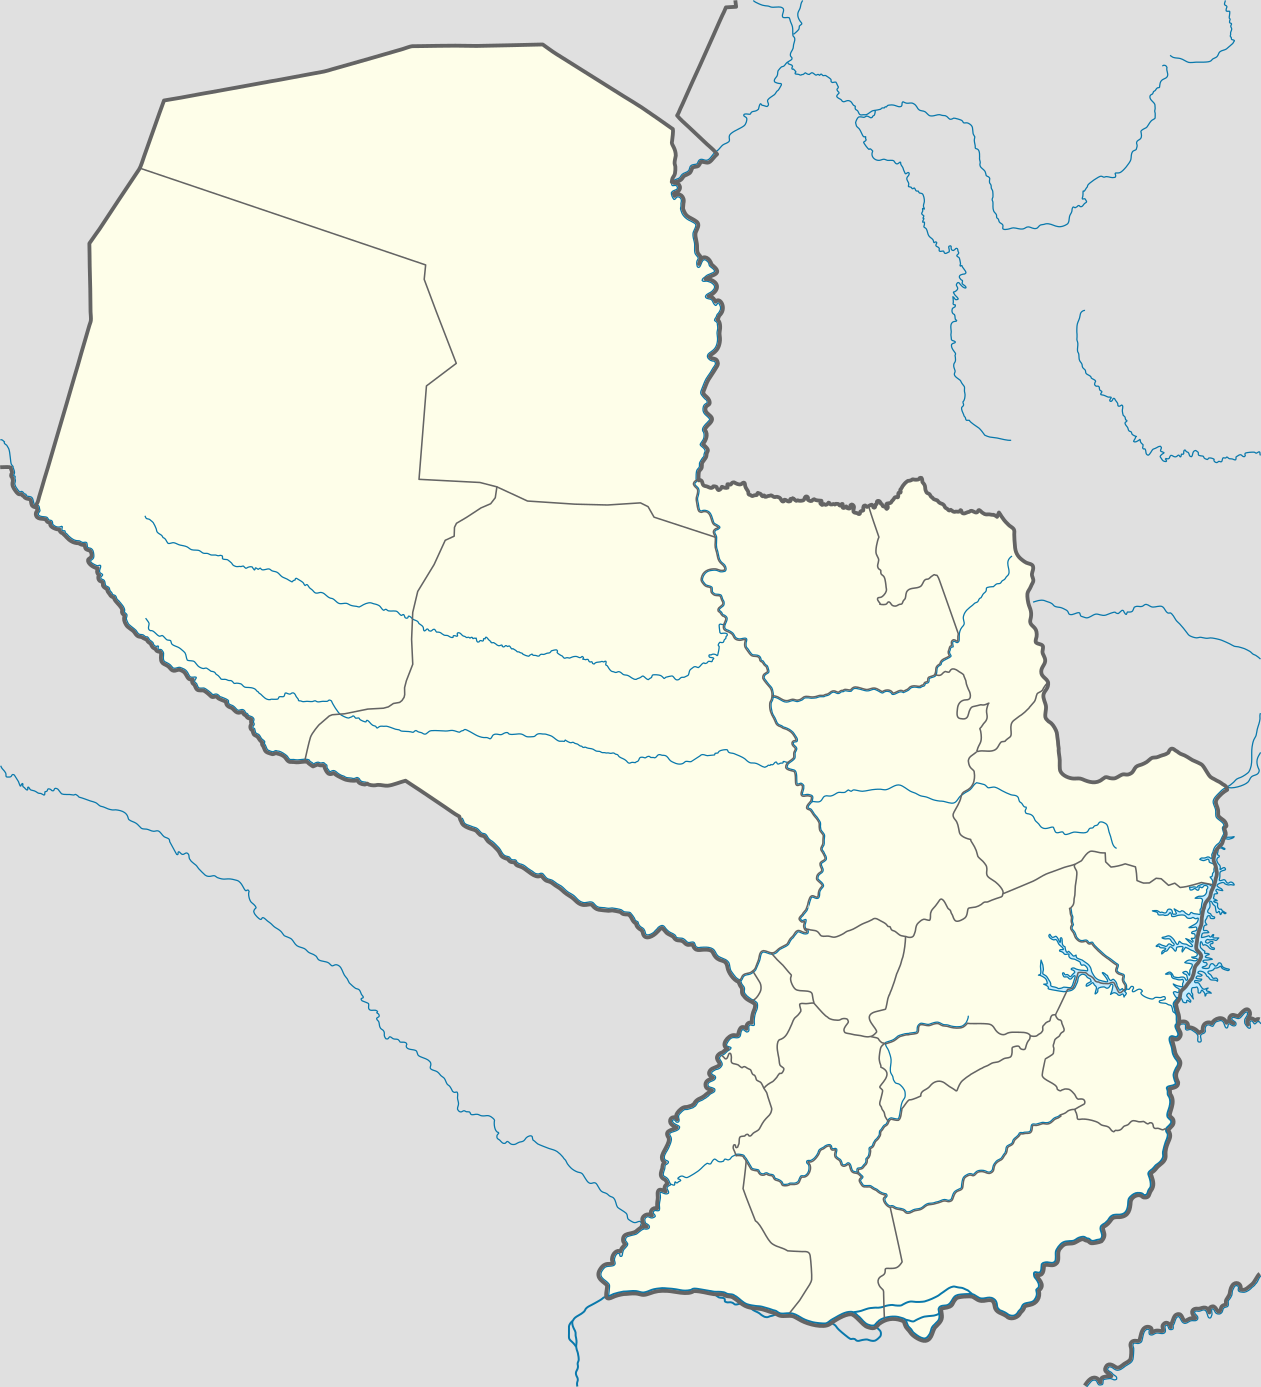
\includegraphics[width=0.65\textwidth]{mapas/paraguai_base.pdf}};
    \begin{scope}[x={(image.south east)}, y={(image.north west)}]
        \ifcase#1
            \def\px{0.56}\def\py{0.40} % 0: Asuncion
        \or \def\px{0.65}\def\py{0.65} % 1: Concepcion
        \or \def\px{0.68}\def\py{0.52} % 2: San Pedro
        \or \def\px{0.62}\def\py{0.40} % 3: Cordillera
        \or \def\px{0.72}\def\py{0.35} % 4: Guaira
        \or \def\px{0.75}\def\py{0.42} % 5: Caaguazu
        \or \def\px{0.75}\def\py{0.28} % 6: Caazapa
        \or \def\px{0.78}\def\py{0.18} % 7: Itapua
        \or \def\px{0.65}\def\py{0.18} % 8: Misiones
        \or \def\px{0.63}\def\py{0.32} % 9: Paraguari
        \or \def\px{0.88}\def\py{0.40} % 10: Alto Parana
        \or \def\px{0.58}\def\py{0.38} % 11: Central
        \or \def\px{0.52}\def\py{0.22} % 12: Neembucu
        \or \def\px{0.82}\def\py{0.72} % 13: Amambay
        \or \def\px{0.85}\def\py{0.55} % 14: Canindeyu
        \or \def\px{0.45}\def\py{0.50} % 15: Pres. Hayes
        \or \def\px{0.25}\def\py{0.75} % 16: Boqueron
        \or \def\px{0.55}\def\py{0.85} % 17: Alto Paraguay
        \fi
        \ifdefined\px
            \draw[red, very thick] (\px,\py) circle (10pt);
            \draw[red, very thick] (\px,\py) circle (2pt);
            \draw[red, thick] (\px-0.05,\py) -- (\px-0.015,\py);
            \draw[red, thick] (\px+0.015,\py) -- (\px+0.05,\py);
            \draw[red, thick] (\px,\py-0.05) -- (\px,\py-0.015);
            \draw[red, thick] (\px,\py+0.015) -- (\px,\py+0.05);
            \node[anchor=west, fill=white, fill opacity=0.7, text opacity=1, inner sep=2pt, rounded corners=2pt] at (\px+0.03, \py) {\tiny\bfseries #2};
        \fi
    \end{scope}
  \end{tikzpicture}
  \end{center}
}

% --- MINI MAPA DO DISTRITO (Refinado) ---
\newcommand{\mapaConteudo}[2]{
    \begin{tikzpicture}
        \node[anchor=south west, inner sep=0] (image) at (0,0) {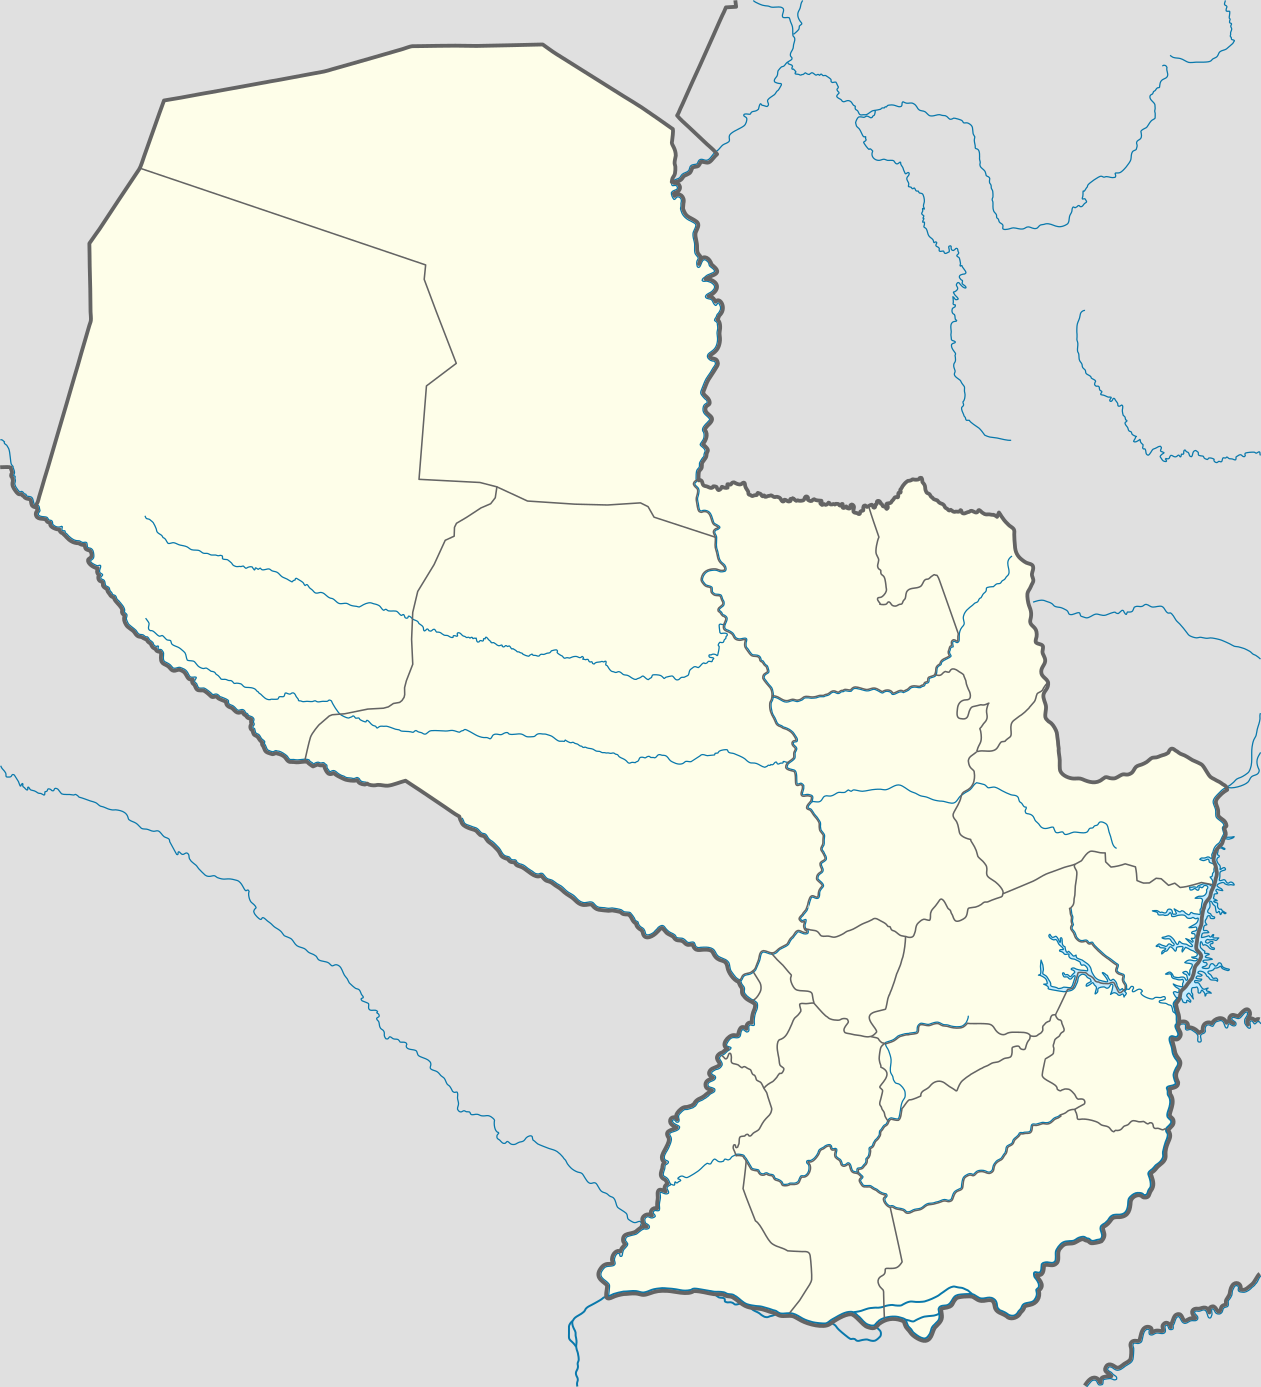
\includegraphics[width=0.33\textwidth]{mapas/paraguai_base.pdf}};
        \begin{scope}[x={(image.south east)}, y={(image.north west)}]
            \pgfmathsetmacro{\xpos}{(#2 + 62.7) / 8.5}
            \pgfmathsetmacro{\ypos}{(#1 + 27.6) / 8.4}
            \fill[red] (\xpos, \ypos) circle (2.5pt);
            \draw[red, thick] (\xpos, \ypos) circle (5pt);
        \end{scope}
    \end{tikzpicture}
}

\newcommand{\secaoDiagnostico}[3]{%
  \section*{#1} % Título da Cidade
  \addcontentsline{toc}{section}{#1}
  \label{dist:#1} % Label para links automáticos
  \noindent\textbf{Diagnóstico Integrado}\par\medskip % Título em largura total
  \begin{wrapfigure}{r}{0.35\textwidth}
    \centering
    \vspace{-10pt} % Ajuste fino de alinhamento
    #2 % Conteúdo do mapa (TikZ ou imagem)
  \end{wrapfigure}
  #3 % Texto e listas que vão contornar o mapa
  \par\vspace{1em}
}

% --- AJUSTE DE SUMÁRIO ---
\usepackage{tocloft}
\advance\cftsecnumwidth 0.5em
\setcounter{tocdepth}{2}

% Títulos
\setcounter{secnumdepth}{-1}
\titleformat{\section}{\Large\bfseries\raggedright}{}{0em}{}
\titleformat{\subsection}{\large\bfseries\raggedright}{}{0em}{}
\titleformat{\subsubsection}{\normalsize\bfseries\raggedright}{}{0em}{}

\sloppy

\providecommand{\tightlist}{%
  \setlength{\itemsep}{0pt}\setlength{\parskip}{0pt}}

\pagestyle{fancy}
\fancyhf{}
\fancyhead[L]{\small Guia Estratégico Paraguai 2026}
\fancyhead[R]{\small \thepage}

\title{\textbf{GUIA ESTRATÉGICO:\\RELOCAÇÃO E SOBREVIVÊNCIA NO PARAGUAI}}
\author{Rodrigo Braga Prado}
\date{Edição Técnica - 2026}

\begin{document}

\maketitle
\tableofcontents

\chapter*{Introdução}
Este guia consolida a análise tática de todos os 262 distritos do Paraguai, aplicando a metodologia Skousen adaptada e dados demográficos do Censo 2022.

% =====================================================================
% METODOLOGIA GSS — Versão 2.0 (Artefato Central AC-01)
% Global Safety Score aplicado ao Paraguai
% =====================================================================
\chapter*{Metodologia}
\addcontentsline{toc}{chapter}{Metodologia}

\section{Origem e Adaptação do Método}

A metodologia que sustenta este guia deriva do trabalho pioneiro de Joel Skousen, arquiteto e analista geopolítico norte-americano, cujo livro \textit{Strategic Relocation: North American Guide to Safe Places} (1997, com revisões em 2011 e 2020) estabeleceu pela primeira vez um framework sistemático para avaliar a segurança de localidades sob múltiplas dimensões simultâneas. Skousen priorizou, em seu modelo original, as ameaças estratégicas e militares — reflexo do contexto da Guerra Fria e da preocupação com alvos nucleares nos Estados Unidos — e as combinou com análise de densidade populacional, recursos naturais e estabilidade política.

A presente versão, denominada \textbf{Global Safety Score (GSS)}, expande e recalibra esse framework para o contexto sul-americano do século XXI, com as seguintes adaptações fundamentais:

\begin{itemize}
  \item \textbf{Tropicalização dos critérios climáticos}: o modelo original foi concebido para zonas temperadas do hemisfério norte. O Paraguai possui dinâmicas de seca, inundação sazonal e calor extremo que exigem variáveis específicas.
  \item \textbf{Operacionalização com dados abertos}: cada variável do GSS é ligada a uma fonte verificável — Censo DGEEC 2022, NASA POWER, Ministerio Público do Paraguai, INE/EPHC, SoilGrids, Global Data Lab — eliminando avaliações puramente subjetivas.
  \item \textbf{Perfis de leitor}: o modelo padrão de Skousen assume um único perfil de relocado. O GSS introduz seis perfis distintos com pesos ajustados, reconhecendo que um agricultor colono, um investidor imobiliário e uma família preparacionista possuem hierarquias de risco completamente diferentes.
  \item \textbf{Escala de confiança por variável}: cada pontuação carrega um nível de confiança (A, B ou C) que reflete a qualidade do dado subjacente, permitindo ao leitor avaliar a robustez da estimativa.
\end{itemize}

O GSS é, portanto, uma ferramenta de inteligência geográfica aplicada — não uma garantia de segurança, mas um mapa de probabilidades que orienta decisões de alto impacto com a melhor informação disponível.

\section{Estrutura Geral da Pontuação}

Cada localidade recebe uma pontuação em cinco dimensões independentes, todas avaliadas em uma escala de \textbf{0 a 10}, onde \textbf{10 representa o estado ideal} (menor risco, maior aptidão) e \textbf{0 representa o estado crítico} (risco máximo ou inviabilidade).

A pontuação final GSS é uma média ponderada dessas cinco dimensões:

\begin{equation}
\mathrm{GSS} = \frac{(A \times w_A) + (B \times w_B) + (C \times w_C) + (D \times w_D) + (E \times w_E)}{10}
\end{equation}

Na configuração padrão (perfil neutro), os pesos são:

\begin{equation}
\mathrm{GSS}_{\mathrm{padr\tilde{a}o}} = \frac{(A \times 2{,}5) + (B \times 2{,}0) + (C \times 1{,}5) + (D \times 2{,}0) + (E \times 2{,}0)}{10}
\end{equation}

A restrição de consistência exige que a soma dos pesos seja sempre igual à unidade:

\begin{equation}
w_A + w_B + w_C + w_D + w_E = 1{,}00
\end{equation}

As cinco dimensões são:

\begin{itemize}
  \item \textbf{A — Ameaças Estratégicas e Militares} (peso padrão: 25\%)
  \item \textbf{B — Risco Social} (peso padrão: 20\%)
  \item \textbf{C — Riscos Naturais e Clima} (peso padrão: 15\%)
  \item \textbf{D — Autossuficiência e Recursos} (peso padrão: 20\%)
  \item \textbf{E — Ambiente Institucional} (peso padrão: 20\%)
\end{itemize}

As seções seguintes detalham cada dimensão: as variáveis que a compõem, os critérios de pontuação, as fontes de dados e o contexto específico do Paraguai.

% =====================================================================
\section{Dimensão A — Ameaças Estratégicas e Militares}
% =====================================================================

\subsection{Fundamento e Relevância para o Paraguai}

A dimensão A avalia o risco de uma localidade ser diretamente impactada por conflitos armados de escala regional ou global — seja como alvo primário de ataque, seja por efeitos colaterais (fallout, disrupção logística, fluxo de refugiados). No modelo de Skousen, esta é a dimensão mais crítica porque seus efeitos são irreversíveis e de rápido desenvolvimento.

Para o Paraguai, o contexto é estruturalmente favorável: o país é \textit{landlocked} (sem litoral), não possui armas nucleares, não integra nenhuma aliança militar ofensiva (como OTAN ou equivalente regional), e sua posição geopolítica central na América do Sul o coloca fora das rotas de projeção de poder das grandes potências. A pontuação da dimensão A para a maioria dos distritos paraguaios situa-se entre \textbf{7,0 e 9,0}, tornando-o um dos territórios mais favoráveis da América Latina sob este critério.

\subsection{Variáveis Operacionalizadas}

\subsubsection{A1 — Proximidade de Alvos Estratégicos}

Bases militares ativas, usinas hidrelétricas de grande porte, centros de comando governamental e infraestrutura crítica de energia e comunicações constituem alvos prioritários em cenários de conflito. A penalização é proporcional à distância:

\begin{itemize}
  \item \textbf{$< 20$ km de alvo crítico}: penalização severa (escore A1 $\leq$ 4,0)
  \item \textbf{20–50 km}: penalização moderada (A1 entre 4,0 e 6,5)
  \item \textbf{50–150 km}: penalização leve (A1 entre 6,5 e 8,0)
  \item \textbf{$> 150$ km}: sem penalização (A1 entre 8,0 e 10,0)
\end{itemize}

No contexto paraguaio, os alvos estratégicos relevantes são: \textbf{Itaipu Binacional} (Alto Paraná — maior usina hidrelétrica do mundo em geração acumulada), \textbf{Yacyretá} (Misiones/Neembucú — fronteira com Argentina), e o \textbf{Comando de las Fuerzas Militares} em Assunção. Distritos a menos de 30 km de Itaipu recebem penalização explícita nesta variável.

\subsubsection{A2 — Rotas de Invasão e Corredores Geopolíticos}

O Paraguai perdeu a Guerra da Tríplice Aliança (1864–1870) em parte por estar encravado entre Argentina, Brasil e Bolívia, com fronteiras terrestres permeáveis. Historicamente, as rotas de acesso militar privilegiam: o corredor leste (da Tríplice Fronteira ao interior via Alto Paraná), o eixo sul via Misiones/Neembucú (fronteira argentina) e o norte via Concepción (fronteira com Brasil pelo Mato Grosso do Sul).

Localidades afastadas dessas rotas, no interior dos departamentos centrais (Paraguarí, Guairá, Caazapá) ou no Chaco central (Presidente Hayes, Boquerón), recebem bonificação por isolamento estratégico.

\subsubsection{A3 — Risco de Fallout e Contaminação Regional}

Em cenários de conflito com uso de armas químicas, radiológicas ou biológicas no Brasil, Argentina ou Bolívia, a direção predominante dos ventos determina a dispersão. Os ventos predominantes no Paraguai são de nordeste (regime de ventos alisios) e de sul (frentes polares). Localidades no quadrante sudoeste do país, favorecidas pela direção de evacuação de ar, recebem pontuação levemente superior nesta variável.

O risco de contaminação química por acidentes industriais — e não por conflito intencional — é também considerado: o corredor sojicultor do leste (Alto Paraná, Itapúa, Canindeyú) apresenta alta carga de agrotóxicos, o que não é penalizado nesta dimensão A (esse impacto é capturado na dimensão C).

\subsubsection{A4 — Presença de Narcotráfico com Dimensão Militar}

Grupos como o PCC (Primeiro Comando da Capital, oriundo do Brasil) e o Clan Rotela operam no Paraguai com estrutura logística que inclui armamento pesado e capacidade de enfrentamento com forças estatais. A faixa de fronteira com o Brasil — especialmente Amambay (Pedro Juan Caballero), Canindeyú e norte de Alto Paraná — é classificada como zona de atenção sob a perspectiva de ameaças organizadas com capacidade militar informal.

\subsection{Pontuação Final da Dimensão A}

A pontuação da dimensão A é a média ponderada de A1 (50\%), A2 (25\%), A3 (15\%) e A4 (10\%). Para a maioria dos distritos paraguaios fora das zonas de fronteira e das imediações das usinas, o escore A situa-se entre 7,5 e 9,0 — refletindo a posição estruturalmente vantajosa do país.

% =====================================================================
\section{Dimensão B — Risco Social}
% =====================================================================

\subsection{Fundamento e Relevância para o Paraguai}

O risco social avalia a probabilidade de que a vida cotidiana seja perturbada por criminalidade, violência organizada, instabilidade civil ou colapso da coesão comunitária. Para imigrantes e investidores, esta é frequentemente a dimensão de maior impacto imediato sobre a qualidade de vida.

O Paraguai apresenta grande heterogeneidade regional: Assunção e a região metropolitana do Departamento Central concentram a maior parte da criminalidade urbana, enquanto distritos rurais nos departamentos de Misiones, Paraguarí e Caazapá registram taxas de homicídio comparáveis às de países europeus. A análise por distrito é, portanto, indispensável — médias nacionais são enganosas.

\subsection{Variáveis Operacionalizadas}

\subsubsection{B1 — Taxa de Homicídios (por 100 mil habitantes)}

Fonte primária: Ministerio Público del Paraguay — Dirección de Estadísticas (dados anuais por departamento, com série desde 2010). Para distritos, utiliza-se interpolação proporcional à população quando dados desagregados não estão disponíveis.

Critérios de pontuação:

\begin{itemize}
  \item \textbf{$< 3{,}0$/100k}: 9,0–10,0 (equivalente à taxa europeia)
  \item \textbf{3,0–8,0/100k}: 7,0–8,9 (baixo risco)
  \item \textbf{8,0–15,0/100k}: 5,0–6,9 (risco moderado)
  \item \textbf{15,0–25,0/100k}: 3,0–4,9 (risco elevado)
  \item \textbf{$> 25{,}0$/100k}: $< 3{,}0$ (risco crítico — nível de zona de guerra regional)
\end{itemize}

\subsubsection{B2 — Distância de Grandes Centros Populacionais}

Cidades com mais de 500 mil habitantes geram externalidades negativas de segurança: mercados criminais mais desenvolvidos, rotas de tráfico, pressão de refugiados em crises, e saturação de serviços públicos em emergências. No Paraguai, apenas a Área Metropolitana de Assunção (AMA) ultrapassa esse limiar.

\begin{itemize}
  \item \textbf{$> 150$ km da AMA}: bonificação máxima (B2 = 9,0–10,0)
  \item \textbf{80–150 km}: bonificação moderada (B2 = 7,0–8,9)
  \item \textbf{30–80 km}: neutro (B2 = 5,0–6,9)
  \item \textbf{$< 30$ km}: penalização (B2 $\leq$ 4,9)
\end{itemize}

\subsubsection{B3 — Presença de Crime Organizado Transnacional}

O mapeamento considera a documentação pública de operações do \textbf{PCC}, \textbf{Comando Vermelho (CV)}, \textbf{MS-13} e do \textbf{Clan Rotela} no território paraguaio. Fontes: relatórios do InSight Crime (2022–2024), do Ministerio del Interior e da SENAD (Secretaría Nacional Antidrogas).

A presença confirmada de estrutura operacional (não apenas trânsito eventual) de grupos transnacionais resulta em penalização de até 2,0 pontos na variável B3.

\subsubsection{B4 — Índice de Gini e Desigualdade como Proxy de Instabilidade}

Sociedades com alta desigualdade de renda são estruturalmente mais propensas a agitação social e criminalidade predatória. Fonte: INE — EPHC (Encuesta Permanente de Hogares Continua) 2023, desagregada por departamento.

\subsubsection{B5 — Percentual de Pobreza Extrema}

Complementar ao Gini, a pobreza extrema ($< 1$ dólar/dia ajustado) indica vulnerabilidade estrutural da população local. Fonte: INE/EPHC 2023.

\subsubsection{B6 — Superlotação Prisional como Proxy de Saturação Sistêmica}

A taxa de superlotação do sistema prisional regional indica o grau de saturação das instituições de segurança pública — um preditor de recidiva, gangues prisionais e ineficácia policial. Fonte: Ministerio de Justicia del Paraguay.

% =====================================================================
\section{Dimensão C — Riscos Naturais e Clima}
% =====================================================================

\subsection{Fundamento e Relevância para o Paraguai}

O Paraguai não está localizado em zona sísmica ativa, não possui vulcões e não enfrenta risco de tsunami — o que confere ao país uma vantagem estrutural significativa na dimensão C em comparação com países do Pacífico sul-americano (Peru, Chile, Equador, Colômbia). O principal risco natural paraguaio é a variabilidade hídrica extrema: secas prolongadas no Chaco e inundações sazonais severas nas planícies do rio Paraguai e rio Paraná.

\subsection{Variáveis Operacionalizadas}

\subsubsection{C1 — Risco de Inundações}

Fonte: SEAM (Secretaría del Ambiente) e dados hidrológicos do Sistema Nacional de Alerta Hidrometeorológica. Áreas de planície ripária dos rios Paraguai e Paraná, e dos rios Tebicuary, Ypané e Jejuí, são classificadas por frequência de inundação histórica (período de retorno de 5, 10, 25 e 50 anos).

Distritos com mais de 20\% do território em zona de inundação com período de retorno $\leq 10$ anos recebem penalização severa (C1 $\leq$ 4,0). Exemplos: Ñeembucú (Pilar), Concepción (Bella Vista Norte), região do Pantanal no Alto Paraguai.

\subsubsection{C2 — Suscetibilidade a Seca Severa}

Precipitação anual abaixo de 800 mm é o limiar crítico para agricultura de sequeiro e recarga de aquíferos rasos. O Chaco paraguaio registra médias de 400–700 mm anuais com alta variabilidade interanual (coeficiente de variação $> 35\%$). Fonte: NASA POWER (série 2001–2020, parâmetro PRECTOTCORR).

\begin{itemize}
  \item \textbf{$> 1.400$ mm/ano}: 9,0–10,0
  \item \textbf{1.100–1.400 mm/ano}: 7,5–8,9
  \item \textbf{800–1.100 mm/ano}: 5,5–7,4
  \item \textbf{500–800 mm/ano}: 3,0–5,4
  \item \textbf{$< 500$ mm/ano}: $< 3{,}0$
\end{itemize}

\subsubsection{C3 — Risco Sísmico}

O Paraguai está sobre o Cráton do Rio de la Plata, uma das formações geológicas mais estáveis do planeta. O risco sísmico é classificado como mínimo (PGA $< 0{,}04g$ para período de retorno de 475 anos, conforme USGS Hazard Map). Todos os distritos paraguaios recebem bônus fixo de C3 = 9,5 nesta variável, contribuindo positivamente para a dimensão C.

\subsubsection{C4 — Temperatura Extrema e Estresse Térmico}

O Chaco paraguaio registra temperaturas de pico de 42–46°C no verão (novembro–fevereiro), com sensação térmica agravada pela umidade nos meses de chuva. Esses extremos comprometem a produtividade humana, aumentam consumo energético e afetam a pecuária e a agricultura. Fonte: NASA POWER (parâmetro T2M\_MAX, média dos máximos mensais, série 2001–2020).

Distritos com temperatura máxima média anual superior a 38°C recebem penalização de C4 $\leq$ 5,0. A Região Oriental (leste do rio Paraguai) apresenta condições mais moderadas, com máximas médias de 28–34°C.

\subsubsection{C5 — Irradiação Solar Média Anual}

A irradiação solar (GHI — Global Horizontal Irradiance) determina o potencial de geração fotovoltaica e influencia a produtividade agrícola. O Paraguai apresenta excelente irradiação em todo o território: 5,0–6,2 kWh/m²/dia. Fonte: NASA POWER (parâmetro ALLSKY\_SFC\_SW\_DWN).

Esta variável é considerada positiva na dimensão C (maior irradiação = maior potencial energético autônomo) e também é utilizada como componente da dimensão D (autossuficiência energética).

% =====================================================================
\section{Dimensão D — Autossuficiência e Recursos}
% =====================================================================

\subsection{Fundamento e Relevância para o Paraguai}

A dimensão D avalia a capacidade de uma localidade sustentar vida humana com alta qualidade e baixa dependência de cadeias de abastecimento externas. Para relocados que buscam autonomia agrícola, energética e hídrica, esta é frequentemente a dimensão decisiva. O Paraguai destaca-se positivamente aqui: solo fértil em boa parte da Região Oriental, Aquífero Guaraní no subsolo da região leste, irradiação solar excepcional e energia elétrica estatal entre as mais baratas do mundo.

\subsection{Variáveis Operacionalizadas}

\subsubsection{D1 — Qualidade do Solo}

Fonte: SoilGrids (ISRIC — World Soil Information), resolução de 250m, parâmetros: pH (horizonte 0–30 cm), teor de matéria orgânica, textura (percentual de argila, silte e areia) e capacidade de troca catiônica (CEC). Para o Paraguai, os solos mais produtivos concentram-se nos departamentos de Itapúa (terra roxa, análoga ao Paraná brasileiro), Caaguazú e Alto Paraná.

Escala de pontuação D1 baseada em aptidão agrícola (classes FAO):

\begin{itemize}
  \item \textbf{Solo Classe I–II} (muito apto, sem restrições ou restrições leves): D1 = 8,5–10,0
  \item \textbf{Solo Classe III} (apto com restrições moderadas): D1 = 6,5–8,4
  \item \textbf{Solo Classe IV} (apto com restrições severas): D1 = 4,5–6,4
  \item \textbf{Solo Classe V–VI} (marginalmente apto): D1 = 2,5–4,4
  \item \textbf{Solo Classe VII–VIII} (inapto para lavoura): D1 $\leq$ 2,4
\end{itemize}

\subsubsection{D2 — Aquífero e Acesso à Água Subterrânea}

O Aquífero Guaraní, o maior reservatório de água doce subterrânea do planeta, cobre aproximadamente 70\% do território da Região Oriental paraguaia. Distritos sobre o Guaraní recebem bônus de D2 = 9,0–10,0. Fora de sua área de ocorrência (Chaco e extremo norte), a profundidade de poço é a variável determinante: poços rasos ($< 30$ m) são vulneráveis a contaminação e seca; poços artesianos profundos ($> 100$ m) conferem autonomia. Fonte: ORSAS (Organismo Regulador de Saneamiento y Agua, PY) e SENASA.

\subsubsection{D3 — Irradiação Solar para Geração Fotovoltaica}

A disponibilidade de energia solar autônoma é crítica para propriedades rurais fora da rede elétrica ou como redundância em crises de fornecimento. Fonte: NASA POWER (GHI, série 2001–2020). O Paraguai apresenta condições uniformemente boas em todo o território (5,0–6,2 kWh/m²/dia), com destaque para o Chaco central (6,0–6,2 kWh/m²/dia) — ironicamente compensando parcialmente as desvantagens climáticas dessa região.

\subsubsection{D4 — Acesso a Água Potável}

Percentual de domicílios com acesso a água potável canalizada (rede pública ou poço protegido). Fonte: DGEEC — Censo Nacional de Población y Viviendas 2022 (tabelas por distrito). Distritos com cobertura $> 90\%$ recebem D4 = 8,5–10,0; cobertura $< 50\%$ recebe D4 $\leq$ 4,0.

\subsubsection{D5 — Aptidão Agrícola do Território}

Percentual do território distrital em classes de aptidão I–III (aptas para lavoura anual ou permanente), derivado do cruzamento de dados INDERT (Instituto Nacional de Desarrollo Rural y de la Tierra) e classificação SEAM. Distritos com $> 60\%$ do território em classes I–III recebem bonificação de D5 $\geq$ 8,0.

% =====================================================================
\section{Dimensão E — Ambiente Institucional}
% =====================================================================

\subsection{Fundamento e Relevância para o Paraguai}

A dimensão E avalia a qualidade do ambiente institucional — o conjunto de regras formais e informais que determinam a segurança jurídica da propriedade, o acesso a serviços essenciais (saúde, educação, internet) e a estabilidade do sistema político-fiscal. Para imigrantes e investidores estrangeiros, esta dimensão é frequentemente a mais relevante no médio e longo prazo.

O Paraguai apresenta vantagens institucionais estruturais que o distinguem favoravelmente na região: sistema fiscal competitivo (IR pessoal máximo de 10\%, IR corporativo de 10\%, IR agropecuário reduzido), Constituição vigente desde 1992 sem rupturas, e reconhecimento internacional da propriedade privada estrangeira. As desvantagens incluem corrupção persistente no nível municipal e estadual, judiciário lento e IDH entre os mais baixos da América do Sul.

\subsection{Variáveis Operacionalizadas}

\subsubsection{E1 — Índice de Desenvolvimento Humano (IDH) Departamental}

Fonte: Global Data Lab (GDL) — Subnational Human Development Index, série 2022. O IDH integra longevidade, educação e renda em um único indicador. No Paraguai, o IDH departamental varia de aproximadamente 0,620 (Alto Paraguai) a 0,780 (Central/Assunção), com média nacional de 0,717 (PNUD 2023).

\begin{itemize}
  \item \textbf{IDH $\geq$ 0,750}: E1 = 8,5–10,0
  \item \textbf{IDH 0,700–0,749}: E1 = 6,5–8,4
  \item \textbf{IDH 0,650–0,699}: E1 = 4,5–6,4
  \item \textbf{IDH $< 0{,}650$}: E1 $\leq$ 4,4
\end{itemize}

\subsubsection{E2 — Cobertura de Internet Banda Larga}

Percentual de domicílios com acesso a internet (qualquer tecnologia). Fonte: INE — EPHC (Encuesta Permanente de Hogares Continua) 2023, por departamento. Para nômades digitais, profissionais remotos e qualquer pessoa dependente de conectividade, esta variável é decisiva. A cobertura de fibra ótica no Paraguai concentra-se na Área Metropolitana de Assunção e nos principais centros departamentais; o interior rural ainda depende de 4G com cobertura variável. Fonte complementar: CONATEL (Comisión Nacional de Telecomunicaciones) — mapas de cobertura 2024.

\subsubsection{E3 — Segurança Jurídica e Proteção à Propriedade}

O Paraguai permite que estrangeiros possuam propriedade rural e urbana nos mesmos termos que cidadãos nacionais, com registro em cartório (Registros Públicos) de eficácia jurídica reconhecida. A legislação de propriedade intelectual e contratos é baseada no Código Civil Paraguaio de 1987, com reformas em 2012 e 2020. O sistema de registro imobiliário apresenta vulnerabilidades em áreas rurais remotas, onde títulos sobrepostos e disputas com comunidades indígenas são documentados.

Penalização específica para distritos com histórico documentado de conflitos fundiários (fonte: INDERT e organizações de direitos humanos: Tierraviva, CODEHUPY).

\subsubsection{E4 — Sistema Tributário: Comparativo com o Brasil}

O regime fiscal paraguaio é um dos diferenciais mais citados por imigrantes brasileiros. Os principais tributos relevantes para relocados são:

\begin{itemize}
  \item \textbf{IRACIS} (Imposto sobre a Renda das Atividades Comerciais, Industriais e de Serviços): alíquota de 10\% sobre lucro líquido.
  \item \textbf{IRAGRO/IMAGRO} (Imposto sobre a Renda das Atividades Agropecuárias): alíquota de 10\% sobre 30\% da renda bruta (efetiva: $\approx$ 3\% da receita bruta) para propriedades $> 300$ ha. Propriedades menores enquadram-se no regime simplificado.
  \item \textbf{IRP} (Imposto sobre a Renda das Pessoas Físicas): alíquota progressiva até 10\%, com mínimo não tributável elevado (aproximadamente 10 salários mínimos/mês).
  \item \textbf{IVA}: alíquota padrão de 10\% (5\% para produtos básicos e medicamentos).
\end{itemize}

Comparativamente ao Brasil, onde a carga tributária efetiva sobre pessoa física pode superar 35\% e o IR empresarial (IRPJ + CSLL) alcança 34\%, o Paraguai representa uma diferença significativa para pessoas físicas com renda moderada a alta e para empreendedores rurais.

\subsubsection{E5 — Estabilidade Política e Institucional}

O Paraguai mantém sua Constituição desde 1992, com eleições presidenciais regulares e transferência pacífica de poder. O país não integra blocos políticos de alto risco geopolítico e possui relações diplomáticas estáveis com os principais parceiros comerciais (Brasil, Argentina, União Europeia, Estados Unidos, Taiwan). A instabilidade política é um risco de médio prazo, concentrado em disputas eleitorais internas ao Partido Colorado (dominante desde 1947), mas sem histórico recente de golpes ou ruptura constitucional.

% =====================================================================
\section{Tabela de Pesos por Perfil de Leitor}
% =====================================================================

O coração operacional do GSS é a possibilidade de ajustar os pesos das dimensões conforme o perfil de quem toma a decisão de relocação. Um agricultor que busca autossuficiência alimentar e um empresário que avalia carga tributária possuem hierarquias de prioridade fundamentalmente distintas — e o GSS deve refletir essas diferenças.

Os seis perfis a seguir foram derivados de entrevistas com imigrantes brasileiros no Paraguai (2023–2024) e de análise das motivações declaradas em fóruns de relocação (Paraguai para Todos, Expats Paraguay, comunidades no Telegram). Cada perfil mantém a restrição $\sum w_i = 1{,}00$.

\medskip

\noindent\textbf{Descrição dos Perfis:}

\begin{description}
  \item[P1 — Colono/Agricultor] Busca terra produtiva, água abundante, clima favorável à produção de alimentos e autonomia energética. Prioriza as dimensões D (solo, aquífero, aptidão agrícola) e C (clima, seca, inundações). Ameaças estratégicas e ambiente institucional têm menor peso relativo.

  \item[P2 — Investidor Imobiliário] Busca retorno financeiro, segurança jurídica do investimento, tributação favorável e valorização patrimonial. Prioriza as dimensões E (segurança jurídica, tributação, IDH) e D (aptidão, infraestrutura, valorização). Risco de conflito armado tem peso mínimo.

  \item[P3 — Profissional Liberal Urbano] Busca qualidade de vida urbana, baixa criminalidade, acesso a serviços e conectividade. Prioriza as dimensões B (segurança, densidade, crime organizado) e E (internet, IDH, serviços). Riscos naturais têm peso intermediário; ameaças estratégicas são secundárias.

  \item[P4 — Família Preparacionista] Busca máxima resiliência em cenários de colapso sistêmico: prioriza A (distância de alvos, rotas de invasão) e D (autossuficiência total — água, solo, energia). Ambiente institucional é secundário; mobilidade e discrição são prioritárias.

  \item[P5 — Nômade Digital / Aposentado] Busca clima agradável, segurança pessoal, custo de vida razoável e conectividade para trabalho remoto ou lazer. Prioriza C (clima), B (segurança) e E (internet). Ameaças estratégicas têm peso mínimo.

  \item[P6 — Empresário / Empreendedor] Busca ambiente fiscal competitivo, segurança jurídica para negócios, acesso a mercado e estabilidade regulatória. Prioriza E (tributação, IDH, institucional) e B (estabilidade, mercado). Clima e ameaças estratégicas têm peso reduzido.
\end{description}

\medskip

\noindent A tabela a seguir consolida os pesos por dimensão para cada perfil:

\medskip

\renewcommand{\arraystretch}{1.4}
\begin{longtable}{@{} l c c c c c c c @{}}
\toprule
\textbf{Dimensão} &
\textbf{Padrão} &
\textbf{P1} &
\textbf{P2} &
\textbf{P3} &
\textbf{P4} &
\textbf{P5} &
\textbf{P6} \\
& & \small{Colono} & \small{Investidor} & \small{Profissional} & \small{Prepper} & \small{Nômade} & \small{Empresário} \\
\midrule
\endfirsthead
\multicolumn{8}{c}{\textit{(continuação)}} \\
\toprule
\textbf{Dimensão} &
\textbf{Padrão} &
\textbf{P1} &
\textbf{P2} &
\textbf{P3} &
\textbf{P4} &
\textbf{P5} &
\textbf{P6} \\
\midrule
\endhead
\bottomrule
\endfoot
\bottomrule
\endlastfoot
A — Ameaças Estratégicas & 25\% & 10\% & 5\% & 10\% & 35\% & 10\% & 5\% \\
B — Risco Social          & 20\% & 20\% & 15\% & 35\% & 15\% & 25\% & 20\% \\
C — Riscos Naturais       & 15\% & 20\% & 15\% & 20\% & 15\% & 25\% & 15\% \\
D — Autossuficiência      & 20\% & 35\% & 25\% & 10\% & 30\% & 15\% & 20\% \\
E — Institucional         & 20\% & 15\% & 40\% & 25\% &  5\% & 25\% & 40\% \\
\midrule
\textbf{Total}            & \textbf{100\%} & \textbf{100\%} & \textbf{100\%} & \textbf{100\%} & \textbf{100\%} & \textbf{100\%} & \textbf{100\%} \\
\end{longtable}

\medskip

Para calcular o GSS personalizado com o perfil P1 (Colono), por exemplo:

\begin{equation}
\mathrm{GSS}_{\mathrm{P1}} = \frac{(A \times 1{,}0) + (B \times 2{,}0) + (C \times 2{,}0) + (D \times 3{,}5) + (E \times 1{,}5)}{10}
\end{equation}

Os multiplicadores (denominados $m_i$) são obtidos multiplicando os pesos percentuais por 10. A restrição é $\sum m_i = 10$ para todos os perfis.

% =====================================================================
\section{Tabela de Classificação GSS}
% =====================================================================

A pontuação GSS final (em qualquer configuração de perfil) é interpretada conforme a seguinte escala de classificação:

\medskip

\renewcommand{\arraystretch}{1.35}
\begin{tabularx}{\textwidth}{@{} c X X @{}}
\toprule
\textbf{Faixa GSS} & \textbf{Classificação} & \textbf{Interpretação Prática} \\
\midrule
9,0 – 10,0 &
\textbf{Santuário de Nível Superior} &
Localidade com vantagens excepcionais em todas as dimensões relevantes. Raro no contexto sul-americano. Recomendação máxima para qualquer perfil de relocado. \\[0.3em]
7,5 – 8,9 &
\textbf{Destino Recomendado com Vantagens Excepcionais} &
Forte desempenho nas dimensões principais. Pode haver limitações em uma ou duas variáveis secundárias. Excelente escolha para a maioria dos perfis. \\[0.3em]
6,5 – 7,4 &
\textbf{Destino Viável com Monitoramento} &
Bom desempenho geral com ressalvas pontuais. Requer planejamento específico para compensar as dimensões abaixo da média. Viável com preparação adequada. \\[0.3em]
5,0 – 6,4 &
\textbf{Moderadamente Seguro — Preparação Intensiva Necessária} &
Desvantagens relevantes em uma ou mais dimensões críticas. Pode ser adequado para perfis específicos (ex.: P2 em área com alta valorização imobiliária e GSS 5,5 na dimensão B). Exige plano de mitigação detalhado. \\[0.3em]
$<$ 5,0 &
\textbf{Zona de Risco — Evitar para Relocação Definitiva} &
Combinação de fatores negativos que torna a relocação permanente inadequada sob a metodologia GSS. Pode ser considerada apenas para operações temporárias com estrutura de saída clara. \\
\bottomrule
\end{tabularx}

\medskip

\noindent\textbf{Nota sobre distribuição no Paraguai:} dos 262 distritos avaliados, nenhum atinge a faixa 9,0–10,0 no perfil padrão — refletindo a ausência de regiões com simultaneidade de excelência em todas as cinco dimensões. A faixa 7,5–8,9 concentra os melhores distritos da Região Oriental (especialmente Misiones, Paraguarí interior e Itapúa sul). A faixa $< 5{,}0$ é predominante no Chaco e em distritos da faixa de fronteira norte com histórico de conflito organizado.

% =====================================================================
\section{Protocolo de Incerteza e Bandas de Confiança}
% =====================================================================

Nenhum sistema de pontuação geográfica opera sem incerteza. A qualidade dos dados varia substancialmente entre variáveis e entre distritos — e essa variação precisa ser comunicada ao leitor de forma transparente. O GSS adota um sistema de três níveis de confiança:

\subsection{Níveis de Confiança}

\textbf{Nível A — Dado Primário Oficial Verificado}

O score deriva de dados coletados diretamente de fontes primárias com metodologia auditável. Exemplos: taxa de homicídios do Ministerio Público PY, precipitação do NASA POWER (série 2001–2020), percentual de acesso à água do Censo DGEEC 2022, IDH do Global Data Lab, irradiação solar do NASA POWER. A margem de erro estimada é $\pm 0{,}3$ pontos no score final da dimensão.

\textbf{Nível B — Estimativa Interpolada de Dados Regionais Oficiais}

O score deriva de dados oficiais disponíveis no nível departamental, interpolados para o nível distrital por modelos de distribuição proporcional (à população, à área ou à densidade). Exemplos: cobertura de internet por distrito (derivada de dados EPHC por departamento), pobreza extrema por distrito (derivada de EPHC departamental + dados Censo 2022). A margem de erro estimada é $\pm 0{,}5$ pontos no score da dimensão.

\textbf{Nível C — Proxy Inferido por Analogia ou Modelo}

O score deriva de variáveis proxy ou de modelos indiretos quando o dado direto não está disponível. Exemplos: qualidade do solo em distritos sem cobertura SoilGrids de alta resolução (inferida por analogia com distritos adjacentes de fisiografia semelhante), profundidade de poço estimada por modelo hidrogeológico simplificado, presença de crime organizado inferida por proximidade a rotas documentadas. A margem de erro estimada é $\pm 1{,}0$ ponto no score da dimensão.

\subsection{Notação de Incerteza nos Scores}

Quando a maioria das variáveis de uma dimensão é classificada como Nível C, ou quando há variáveis de Nível C em dimensões de alto peso no perfil do leitor, o score é apresentado com banda de incerteza explícita:

\begin{itemize}
  \item Score com predominância de Nível A: apresentado como valor simples (ex.: GSS = 7,8)
  \item Score com presença significativa de Nível B: apresentado como valor com nota (ex.: GSS = 7,2$^{\dagger}$)
  \item Score com maioria de variáveis Nível C: apresentado como intervalo (ex.: GSS = 6,4 $\pm$ 0,8)
\end{itemize}

% =====================================================================
\section{Limitações, Transparência e Escopo do GSS}
% =====================================================================

\subsection{O que o GSS NÃO mede}

A honestidade metodológica exige declarar explicitamente o que este sistema \textit{não} avalia:

\begin{itemize}
  \item \textbf{Preço de imóveis e custo de vida}: o GSS não é um índice de custo-benefício imobiliário. Um distrito com GSS 8,5 pode ter terra cara; outro com GSS 6,8 pode oferecer oportunidades excepcionais de preço. O capítulo de cada departamento inclui dados de mercado separadamente.
  \item \textbf{Acesso a educação superior}: universidades e institutos técnicos não são variáveis do GSS. O IDH (E1) captura parcialmente a educação básica, mas não o acesso a formação superior.
  \item \textbf{Burocracia de visto e residência}: o processo migratório legal paraguaio é descrito no capítulo de Migração Legal. O GSS não penaliza ou bonifica localidades por facilidade de regularização migratória.
  \item \textbf{Mercado de trabalho formal}: o GSS é orientado para quem traz renda própria (investimento, aposentadoria, renda passiva, trabalho remoto). Não avalia oportunidades de emprego formal local.
  \item \textbf{Qualidade de serviços de saúde}: serviços de saúde pública paraguaios apresentam qualidade heterogênea. O IDH captura parcialmente a longevidade, mas o GSS não avalia hospitais ou disponibilidade de especialistas por distrito.
  \item \textbf{Dinâmicas culturais e linguísticas}: a integração social de imigrantes — especialmente em comunidades bilíngues guaraní/espanhol — não é quantificável pelo GSS.
\end{itemize}

\subsection{Frequência de Revisão dos Dados}

Os dados do GSS têm diferentes ciclos de atualização:

\begin{itemize}
  \item \textbf{NASA POWER} (clima, irradiação): série histórica 2001–2020, estável. Revisão recomendada a cada 10 anos ou quando novas séries climatológicas forem publicadas.
  \item \textbf{Censo DGEEC 2022}: próximo censo previsto para 2032. Dados de água, saneamento e densidade populacional desta edição são válidos para o período 2022–2030.
  \item \textbf{EPHC/INE} (dados socioeconômicos): pesquisa anual. Scores da dimensão B (risco social) e E (IDH, internet) devem ser revisados anualmente.
  \item \textbf{Ministerio Público} (homicídios): dados anuais. A variável B1 é atualizada anualmente.
  \item \textbf{SoilGrids} (qualidade do solo): produto baseado em modelagem global com atualização irregular. Revisão recomendada com cada nova versão do produto (versão atual: SoilGrids 2.0, 2021).
  \item \textbf{InSight Crime / SENAD} (crime organizado): relatórios anuais. A variável B3 deve ser revisada a cada 12–18 meses.
\end{itemize}

Esta edição utiliza os dados mais recentes disponíveis até dezembro de 2024. Os scores foram calculados entre janeiro e março de 2025.

\subsection{Nota sobre Subjetividade Residual}

Apesar da operacionalização com dados quantitativos, o GSS não elimina completamente o julgamento analítico. A definição dos limiares de pontuação (ex.: qual precipitação corresponde ao score C2 = 5,0?) envolve escolhas que outros analistas poderiam fazer diferentemente. O modelo é transparente sobre esses limiares — todos descritos neste capítulo — para que o leitor possa questionar, ajustar e replicar o raciocínio com seus próprios critérios.

O GSS é uma ferramenta de apoio à decisão, não um oráculo. A decisão final de relocação deve integrar visitas presenciais, conversas com moradores locais e assessoria jurídica especializada.

\section{Capitulos Finais - Paraguay}\label{capitulos-finais---paraguay}

\subsection{Capitulo 1 - Metodologia
aplicada}\label{capitulo-1---metodologia-aplicada}

Consolidacao em 3 ondas: base factual, calibracao quantitativa e produto
editorial/\allowbreak publicacao.

\subsection{Capitulo 2 - Panorama
nacional}\label{capitulo-2---panorama-nacional}

Total de distritos avaliados: 262.

\subsection{Capitulo 3 - Departamentos (media
GSS)}\label{capitulo-3---departamentos-media-gss}

\begin{itemize}
\tightlist
\item
  \begin{enumerate}
  \def\labelenumi{\arabic{enumi}.}
  \tightlist
  \item
    \hyperref[dept:Amambay]{Amambay} 7.20 (6 distritos)
  \end{enumerate}
\item
  \begin{enumerate}
  \def\labelenumi{\arabic{enumi}.}
  \setcounter{enumi}{1}
  \tightlist
  \item
    \hyperref[dept:Alto Paraguay]{Alto Paraguay} 7.20 (4 distritos)
  \end{enumerate}
\item
  \begin{enumerate}
  \def\labelenumi{\arabic{enumi}.}
  \setcounter{enumi}{2}
  \tightlist
  \item
    \hyperref[dept:Caazapa]{Caazapa} 7.11 (11 distritos)
  \end{enumerate}
\item
  \begin{enumerate}
  \def\labelenumi{\arabic{enumi}.}
  \setcounter{enumi}{3}
  \tightlist
  \item
    \hyperref[dept:Paraguari]{Paraguari} 7.08 (18 distritos)
  \end{enumerate}
\item
  \begin{enumerate}
  \def\labelenumi{\arabic{enumi}.}
  \setcounter{enumi}{4}
  \tightlist
  \item
    \hyperref[dept:San Pedro]{San Pedro} 7.07 (22 distritos)
  \end{enumerate}
\item
  \begin{enumerate}
  \def\labelenumi{\arabic{enumi}.}
  \setcounter{enumi}{5}
  \tightlist
  \item
    \hyperref[dept:Cordillera]{Cordillera} 7.02 (19 distritos)
  \end{enumerate}
\item
  \begin{enumerate}
  \def\labelenumi{\arabic{enumi}.}
  \setcounter{enumi}{6}
  \tightlist
  \item
    \hyperref[dept:Neembucu]{Neembucu} 6.95 (16 distritos)
  \end{enumerate}
\item
  \begin{enumerate}
  \def\labelenumi{\arabic{enumi}.}
  \setcounter{enumi}{7}
  \tightlist
  \item
    \hyperref[dept:Presidente Hayes]{Presidente Hayes} 6.93 (10 distritos)
  \end{enumerate}
\item
  \begin{enumerate}
  \def\labelenumi{\arabic{enumi}.}
  \setcounter{enumi}{8}
  \tightlist
  \item
    \hyperref[dept:Boqueron]{Boqueron} 6.93 (4 distritos)
  \end{enumerate}
\item
  \begin{enumerate}
  \def\labelenumi{\arabic{enumi}.}
  \setcounter{enumi}{9}
  \tightlist
  \item
    \hyperref[dept:Canindeyu]{Canindeyu} 6.92 (16 distritos)
  \end{enumerate}
\item
  \begin{enumerate}
  \def\labelenumi{\arabic{enumi}.}
  \setcounter{enumi}{10}
  \tightlist
  \item
    \hyperref[dept:Guaira]{Guaira} 6.88 (18 distritos)
  \end{enumerate}
\item
  \begin{enumerate}
  \def\labelenumi{\arabic{enumi}.}
  \setcounter{enumi}{11}
  \tightlist
  \item
    \hyperref[dept:Misiones]{Misiones} 6.88 (10 distritos)
  \end{enumerate}
\item
  \begin{enumerate}
  \def\labelenumi{\arabic{enumi}.}
  \setcounter{enumi}{12}
  \tightlist
  \item
    \hyperref[dept:Alto Parana]{Alto Parana} 6.87 (22 distritos)
  \end{enumerate}
\item
  \begin{enumerate}
  \def\labelenumi{\arabic{enumi}.}
  \setcounter{enumi}{13}
  \tightlist
  \item
    \hyperref[dept:Itapua]{Itapua} 6.78 (30 distritos)
  \end{enumerate}
\item
  \begin{enumerate}
  \def\labelenumi{\arabic{enumi}.}
  \setcounter{enumi}{14}
  \tightlist
  \item
    \hyperref[dept:Caaguazu]{Caaguazu} 6.64 (22 distritos)
  \end{enumerate}
\item
  \begin{enumerate}
  \def\labelenumi{\arabic{enumi}.}
  \setcounter{enumi}{15}
  \tightlist
  \item
    \hyperref[dept:Central]{Central} 6.61 (19 distritos)
  \end{enumerate}
\item
  \begin{enumerate}
  \def\labelenumi{\arabic{enumi}.}
  \setcounter{enumi}{16}
  \tightlist
  \item
    \hyperref[dept:Distrito Capital]{Distrito Capital} 6.50 (1 distritos)
  \end{enumerate}
\item
  \begin{enumerate}
  \def\labelenumi{\arabic{enumi}.}
  \setcounter{enumi}{17}
  \tightlist
  \item
    \hyperref[dept:Concepción]{Concepción} 6.21 (14 distritos)
  \end{enumerate}
\end{itemize}

\subsection{Capitulo 4 - Top 20
nacional}\label{capitulo-4---top-20-nacional}

\begin{itemize}
\tightlist
\item
  \begin{enumerate}
  \def\labelenumi{\arabic{enumi}.}
  \tightlist
  \item
    \hyperref[dist:Altos]{Altos} (\hyperref[dept:Cordillera]{Cordillera}) - GSS 8.9
  \end{enumerate}
\item
  \begin{enumerate}
  \def\labelenumi{\arabic{enumi}.}
  \setcounter{enumi}{1}
  \tightlist
  \item
    \hyperref[dist:Fram]{Fram} (\hyperref[dept:Itapua]{Itapua}) - GSS 8.9
  \end{enumerate}
\item
  \begin{enumerate}
  \def\labelenumi{\arabic{enumi}.}
  \setcounter{enumi}{2}
  \tightlist
  \item
    \hyperref[dist:General Artigas]{General Artigas} (\hyperref[dept:Itapua]{Itapua}) - GSS 8.8
  \end{enumerate}
\item
  \begin{enumerate}
  \def\labelenumi{\arabic{enumi}.}
  \setcounter{enumi}{3}
  \tightlist
  \item
    \hyperref[dist:San Jose de los Arroyos]{San Jose de los Arroyos} (\hyperref[dept:Cordillera]{Cordillera}) - GSS 8.6
  \end{enumerate}
\item
  \begin{enumerate}
  \def\labelenumi{\arabic{enumi}.}
  \setcounter{enumi}{4}
  \tightlist
  \item
    \hyperref[dist:Mbocayaty del Guaira]{Mbocayaty del Guaira} (\hyperref[dept:Guaira]{Guaira}) - GSS 8.6
  \end{enumerate}
\item
  \begin{enumerate}
  \def\labelenumi{\arabic{enumi}.}
  \setcounter{enumi}{5}
  \tightlist
  \item
    \hyperref[dist:Isla Umbu]{Isla Umbu} (\hyperref[dept:Neembucu]{Neembucu}) - GSS 8.6
  \end{enumerate}
\item
  \begin{enumerate}
  \def\labelenumi{\arabic{enumi}.}
  \setcounter{enumi}{6}
  \tightlist
  \item
    \hyperref[dist:Quiindy]{Quiindy} (\hyperref[dept:Paraguari]{Paraguari}) - GSS 8.5
  \end{enumerate}
\item
  \begin{enumerate}
  \def\labelenumi{\arabic{enumi}.}
  \setcounter{enumi}{7}
  \tightlist
  \item
    \hyperref[dist:Yaguarun]{Yaguarun} (\hyperref[dept:Paraguari]{Paraguari}) - GSS 8.5
  \end{enumerate}
\item
  \begin{enumerate}
  \def\labelenumi{\arabic{enumi}.}
  \setcounter{enumi}{8}
  \tightlist
  \item
    \hyperref[dist:San Vicente Pancholo]{San Vicente Pancholo} (\hyperref[dept:San Pedro]{San Pedro}) - GSS 8.3
  \end{enumerate}
\item
  \begin{enumerate}
  \def\labelenumi{\arabic{enumi}.}
  \setcounter{enumi}{9}
  \tightlist
  \item
    \hyperref[dist:Tavarai]{Tavarai} (\hyperref[dept:Caazapa]{Caazapa}) - GSS 8.3
  \end{enumerate}
\item
  \begin{enumerate}
  \def\labelenumi{\arabic{enumi}.}
  \setcounter{enumi}{10}
  \tightlist
  \item
    \hyperref[dist:Santa Rosa del Monday]{Santa Rosa del Monday} (\hyperref[dept:Alto Parana]{Alto Parana}) - GSS 8.2
  \end{enumerate}
\item
  \begin{enumerate}
  \def\labelenumi{\arabic{enumi}.}
  \setcounter{enumi}{11}
  \tightlist
  \item
    \hyperref[dist:Benjamin Aceval]{Benjamin Aceval} (\hyperref[dept:Presidente Hayes]{Presidente Hayes}) - GSS 8.2
  \end{enumerate}
\item
  \begin{enumerate}
  \def\labelenumi{\arabic{enumi}.}
  \setcounter{enumi}{12}
  \tightlist
  \item
    \hyperref[dist:Itapua Poty]{Itapua Poty} (\hyperref[dept:Itapua]{Itapua}) - GSS 8.1
  \end{enumerate}
\item
  \begin{enumerate}
  \def\labelenumi{\arabic{enumi}.}
  \setcounter{enumi}{13}
  \tightlist
  \item
    \hyperref[dist:Acahay]{Acahay} (\hyperref[dept:Paraguari]{Paraguari}) - GSS 8.1
  \end{enumerate}
\item
  \begin{enumerate}
  \def\labelenumi{\arabic{enumi}.}
  \setcounter{enumi}{14}
  \tightlist
  \item
    \hyperref[dist:Nueva Esperanza]{Nueva Esperanza} (\hyperref[dept:Canindeyu]{Canindeyu}) - GSS 8.1
  \end{enumerate}
\item
  \begin{enumerate}
  \def\labelenumi{\arabic{enumi}.}
  \setcounter{enumi}{15}
  \tightlist
  \item
    \hyperref[dist:Fuerte Olimpo]{Fuerte Olimpo} (\hyperref[dept:Alto Paraguay]{Alto Paraguay}) - GSS 8.1
  \end{enumerate}
\item
  \begin{enumerate}
  \def\labelenumi{\arabic{enumi}.}
  \setcounter{enumi}{16}
  \tightlist
  \item
    \hyperref[dist:Paso Horqueta]{Paso Horqueta} (\hyperref[dept:Concepción]{Concepción}) - GSS 8.0
  \end{enumerate}
\item
  \begin{enumerate}
  \def\labelenumi{\arabic{enumi}.}
  \setcounter{enumi}{17}
  \tightlist
  \item
    \hyperref[dist:General Resquin]{General Resquin} (\hyperref[dept:San Pedro]{San Pedro}) - GSS 8.0
  \end{enumerate}
\item
  \begin{enumerate}
  \def\labelenumi{\arabic{enumi}.}
  \setcounter{enumi}{18}
  \tightlist
  \item
    \hyperref[dist:Itacurubi del Rosario]{Itacurubi del Rosario} (\hyperref[dept:San Pedro]{San Pedro}) - GSS 8.0
  \end{enumerate}
\item
  \begin{enumerate}
  \def\labelenumi{\arabic{enumi}.}
  \setcounter{enumi}{19}
  \tightlist
  \item
    \hyperref[dist:Villa del Rosario]{Villa del Rosario} (\hyperref[dept:San Pedro]{San Pedro}) - GSS 8.0
  \end{enumerate}
\end{itemize}

\subsection{Ranking Nacional}\label{ranking-nacional}

\section{Ranking Nacional de Relocação Estratégica -
Paraguai}\label{ranking-nacional-de-relocauxe7uxe3o-estratuxe9gica---paraguai}

Data: 2026-03-06

\begin{longtable}[]{@{}llll@{}}
\toprule\noalign{}
Rank & Departamento & Distrito & GSS \\
\midrule\noalign{}
\endhead
\bottomrule\noalign{}
\endlastfoot
1 & \hyperref[dept:Cordillera]{Cordillera} & \hyperref[dist:Altos]{Altos} & 8.9 \\
2 & \hyperref[dept:Itapua]{Itapua} & \hyperref[dist:Fram]{Fram} & 8.9 \\
3 & \hyperref[dept:Itapua]{Itapua} & \hyperref[dist:General Artigas]{General Artigas} & 8.8 \\
4 & \hyperref[dept:Cordillera]{Cordillera} & \hyperref[dist:San Jose de los Arroyos]{San Jose de los Arroyos} & 8.6 \\
5 & \hyperref[dept:Guaira]{Guaira} & \hyperref[dist:Mbocayaty del Guaira]{Mbocayaty del Guaira} & 8.6 \\
6 & \hyperref[dept:Neembucu]{Neembucu} & \hyperref[dist:Isla Umbu]{Isla Umbu} & 8.6 \\
7 & \hyperref[dept:Paraguari]{Paraguari} & \hyperref[dist:Quiindy]{Quiindy} & 8.5 \\
8 & \hyperref[dept:Paraguari]{Paraguari} & \hyperref[dist:Yaguarun]{Yaguarun} & 8.5 \\
9 & \hyperref[dept:San Pedro]{San Pedro} & \hyperref[dist:San Vicente Pancholo]{San Vicente Pancholo} & 8.3 \\
10 & \hyperref[dept:Caazapa]{Caazapa} & \hyperref[dist:Tavarai]{Tavarai} & 8.3 \\
11 & \hyperref[dept:Alto Parana]{Alto Parana} & \hyperref[dist:Santa Rosa del Monday]{Santa Rosa del Monday} & 8.2 \\
12 & \hyperref[dept:Presidente Hayes]{Presidente Hayes} & \hyperref[dist:Benjamin Aceval]{Benjamin Aceval} & 8.2 \\
13 & \hyperref[dept:Itapua]{Itapua} & \hyperref[dist:Itapua Poty]{Itapua Poty} & 8.1 \\
14 & \hyperref[dept:Paraguari]{Paraguari} & \hyperref[dist:Acahay]{Acahay} & 8.1 \\
15 & \hyperref[dept:Canindeyu]{Canindeyu} & \hyperref[dist:Nueva Esperanza]{Nueva Esperanza} & 8.1 \\
16 & \hyperref[dept:Alto Paraguay]{Alto Paraguay} & \hyperref[dist:Fuerte Olimpo]{Fuerte Olimpo} & 8.1 \\
17 & \hyperref[dept:Concepción]{Concepción} & \hyperref[dist:Paso Horqueta]{Paso Horqueta} & 8.0 \\
18 & \hyperref[dept:San Pedro]{San Pedro} & \hyperref[dist:General Resquin]{General Resquin} & 8.0 \\
19 & \hyperref[dept:San Pedro]{San Pedro} & \hyperref[dist:Itacurubi del Rosario]{Itacurubi del Rosario} & 8.0 \\
20 & \hyperref[dept:San Pedro]{San Pedro} & \hyperref[dist:Villa del Rosario]{Villa del Rosario} & 8.0 \\
21 & \hyperref[dept:Cordillera]{Cordillera} & \hyperref[dist:Caraguatay]{Caraguatay} & 8.0 \\
22 & \hyperref[dept:Cordillera]{Cordillera} & \hyperref[dist:Eusebio Ayala]{Eusebio Ayala} & 8.0 \\
23 & \hyperref[dept:Itapua]{Itapua} & \hyperref[dist:Alto Vera]{Alto Vera} & 8.0 \\
24 & \hyperref[dept:Alto Parana]{Alto Parana} & \hyperref[dist:Hernandarias]{Hernandarias} & 8.0 \\
25 & \hyperref[dept:Alto Parana]{Alto Parana} & \hyperref[dist:San Alberto]{San Alberto} & 8.0 \\
26 & \hyperref[dept:Concepción]{Concepción} & \hyperref[dist:Loreto]{Loreto} & 7.9 \\
27 & \hyperref[dept:San Pedro]{San Pedro} & \hyperref[dist:Capiibary]{Capiibary} & 7.9 \\
28 & \hyperref[dept:Paraguari]{Paraguari} & \hyperref[dist:San Roque Gonzalez]{San Roque Gonzalez} & 7.9 \\
29 & \hyperref[dept:Alto Parana]{Alto Parana} & \hyperref[dist:Domingo Martinez de Irala]{Domingo Martinez de Irala} & 7.9 \\
30 & \hyperref[dept:Neembucu]{Neembucu} & \hyperref[dist:Humaita]{Humaita} & 7.9 \\
31 & \hyperref[dept:San Pedro]{San Pedro} & \hyperref[dist:Tacuati]{Tacuati} & 7.8 \\
32 & \hyperref[dept:Amambay]{Amambay} & \hyperref[dist:Pedro Juan Caballero]{Pedro Juan Caballero} & 7.8 \\
33 & \hyperref[dept:San Pedro]{San Pedro} & \hyperref[dist:San Pedro de Ycuamandiyu]{San Pedro de Ycuamandiyu} & 7.7 \\
34 & \hyperref[dept:Guaira]{Guaira} & \hyperref[dist:Independencia]{Independencia} & 7.7 \\
35 & \hyperref[dept:Caaguazu]{Caaguazu} & \hyperref[dist:Doctor Juan Manuel Frutos]{Doctor Juan Manuel Frutos} & 7.7 \\
36 & \hyperref[dept:Caaguazu]{Caaguazu} & \hyperref[dist:Mariscal Francisco Solano Lopez]{Mariscal Francisco Solano Lopez} & 7.7 \\
37 & \hyperref[dept:Caazapa]{Caazapa} & \hyperref[dist:Fulgencio Yegros]{Fulgencio Yegros} & 7.7 \\
38 & \hyperref[dept:Itapua]{Itapua} & \hyperref[dist:Natalio]{Natalio} & 7.7 \\
39 & \hyperref[dept:Misiones]{Misiones} & \hyperref[dist:San Patricio]{San Patricio} & 7.7 \\
40 & \hyperref[dept:Paraguari]{Paraguari} & \hyperref[dist:Ybytimi]{Ybytimi} & 7.7 \\
41 & \hyperref[dept:Alto Parana]{Alto Parana} & \hyperref[dist:Presidente Franco]{Presidente Franco} & 7.7 \\
42 & \hyperref[dept:Central]{Central} & \hyperref[dist:Villeta]{Villeta} & 7.7 \\
43 & \hyperref[dept:Neembucu]{Neembucu} & \hyperref[dist:Pilar]{Pilar} & 7.7 \\
44 & \hyperref[dept:Neembucu]{Neembucu} & \hyperref[dist:San Juan del Neembucu]{San Juan del Neembucu} & 7.7 \\
45 & \hyperref[dept:Amambay]{Amambay} & \hyperref[dist:Zanja Pyta]{Zanja Pyta} & 7.7 \\
46 & \hyperref[dept:Presidente Hayes]{Presidente Hayes} & \hyperref[dist:Campo Aceval]{Campo Aceval} & 7.7 \\
47 & \hyperref[dept:Boqueron]{Boqueron} & \hyperref[dept:Boqueron]{Boqueron} & 7.7 \\
48 & \hyperref[dept:Guaira]{Guaira} & \hyperref[dist:Borja]{Borja} & 7.6 \\
49 & \hyperref[dept:Guaira]{Guaira} & \hyperref[dist:Numi]{Numi} & 7.6 \\
50 & \hyperref[dept:Paraguari]{Paraguari} & \hyperref[dist:Escobar]{Escobar} & 7.6 \\
51 & \hyperref[dept:Amambay]{Amambay} & \hyperref[dist:Cerro Cora]{Cerro Cora} & 7.6 \\
52 & \hyperref[dept:Canindeyu]{Canindeyu} & \hyperref[dist:Maracana]{Maracana} & 7.6 \\
53 & \hyperref[dept:San Pedro]{San Pedro} & \hyperref[dist:Nueva Germania]{Nueva Germania} & 7.5 \\
54 & \hyperref[dept:Guaira]{Guaira} & \hyperref[dist:Tebicuary]{Tebicuary} & 7.5 \\
55 & \hyperref[dept:Itapua]{Itapua} & \hyperref[dist:Yatytay]{Yatytay} & 7.5 \\
56 & \hyperref[dept:Alto Parana]{Alto Parana} & \hyperref[dist:Minga Pora]{Minga Pora} & 7.5 \\
57 & \hyperref[dept:Alto Parana]{Alto Parana} & \hyperref[dist:San Cristobal]{San Cristobal} & 7.5 \\
58 & \hyperref[dept:Central]{Central} & \hyperref[dist:Nemby]{Nemby} & 7.5 \\
59 & \hyperref[dept:Neembucu]{Neembucu} & \hyperref[dist:Desmochados]{Desmochados} & 7.5 \\
60 & \hyperref[dept:Canindeyu]{Canindeyu} & \hyperref[dist:Katuete]{Katuete} & 7.5 \\
61 & \hyperref[dept:Canindeyu]{Canindeyu} & \hyperref[dist:Ypejhu]{Ypejhu} & 7.5 \\
62 & \hyperref[dept:Guaira]{Guaira} & \hyperref[dist:Felix Perez Cardozo]{Felix Perez Cardozo} & 7.4 \\
63 & \hyperref[dept:Guaira]{Guaira} & \hyperref[dist:Iturbe]{Iturbe} & 7.4 \\
64 & \hyperref[dept:Caazapa]{Caazapa} & \hyperref[dist:Abai]{Abai} & 7.4 \\
65 & \hyperref[dept:Caazapa]{Caazapa} & \hyperref[dist:Maciel]{Maciel} & 7.4 \\
66 & \hyperref[dept:Itapua]{Itapua} & \hyperref[dist:General Delgado]{General Delgado} & 7.4 \\
67 & \hyperref[dept:Itapua]{Itapua} & \hyperref[dist:Nueva Alborada]{Nueva Alborada} & 7.4 \\
68 & \hyperref[dept:Paraguari]{Paraguari} & \hyperref[dist:Sapucai]{Sapucai} & 7.4 \\
69 & \hyperref[dept:Paraguari]{Paraguari} & \hyperref[dist:Tebicuary mi]{Tebicuary mi} & 7.4 \\
70 & \hyperref[dept:Central]{Central} & \hyperref[dist:Itaugua]{Itaugua} & 7.4 \\
71 & \hyperref[dept:Canindeyu]{Canindeyu} & \hyperref[dist:Yasy Cany]{Yasy Cany} & 7.4 \\
72 & \hyperref[dept:Presidente Hayes]{Presidente Hayes} & \hyperref[dist:Puerto Pinasco]{Puerto Pinasco} & 7.4 \\
73 & \hyperref[dept:Alto Paraguay]{Alto Paraguay} & \hyperref[dist:Puerto Casado]{Puerto Casado} & 7.4 \\
74 & \hyperref[dept:San Pedro]{San Pedro} & \hyperref[dist:Itacurubi]{Itacurubi} & 7.3 \\
75 & \hyperref[dept:Cordillera]{Cordillera} & \hyperref[dist:Piribebuy]{Piribebuy} & 7.3 \\
76 & \hyperref[dept:Guaira]{Guaira} & \hyperref[dist:Yataity del Guaira]{Yataity del Guaira} & 7.3 \\
77 & \hyperref[dept:Caaguazu]{Caaguazu} & \hyperref[dist:Doctor Cecilio Baez]{Doctor Cecilio Baez} & 7.3 \\
78 & \hyperref[dept:Caaguazu]{Caaguazu} & \hyperref[dist:Simon Bolivar]{Simon Bolivar} & 7.3 \\
79 & \hyperref[dept:Caazapa]{Caazapa} & \hyperref[dist:3 de Mayo]{3 de Mayo} & 7.3 \\
80 & \hyperref[dept:Itapua]{Itapua} & \hyperref[dist:Tomas Romero Pereira]{Tomas Romero Pereira} & 7.3 \\
81 & \hyperref[dept:Misiones]{Misiones} & \hyperref[dist:Ayolas]{Ayolas} & 7.3 \\
82 & \hyperref[dept:Paraguari]{Paraguari} & \hyperref[dist:Quyquyho]{Quyquyho} & 7.3 \\
83 & \hyperref[dept:Alto Parana]{Alto Parana} & \hyperref[dist:Tavapy]{Tavapy} & 7.3 \\
84 & \hyperref[dept:Central]{Central} & \hyperref[dist:Lambare]{Lambare} & 7.3 \\
85 & \hyperref[dept:Neembucu]{Neembucu} & \hyperref[dist:Mayor Martinez]{Mayor Martinez} & 7.3 \\
86 & \hyperref[dept:San Pedro]{San Pedro} & \hyperref[dist:Guayaibi]{Guayaibi} & 7.2 \\
87 & \hyperref[dept:Cordillera]{Cordillera} & \hyperref[dist:Caacupe]{Caacupe} & 7.2 \\
88 & \hyperref[dept:Cordillera]{Cordillera} & \hyperref[dist:Tobati]{Tobati} & 7.2 \\
89 & \hyperref[dept:Caaguazu]{Caaguazu} & \hyperref[dist:Nueva Londres]{Nueva Londres} & 7.2 \\
90 & \hyperref[dept:Misiones]{Misiones} & \hyperref[dist:San Miguel]{San Miguel} & 7.2 \\
91 & \hyperref[dept:Misiones]{Misiones} & \hyperref[dist:Yabebyry]{Yabebyry} & 7.2 \\
92 & \hyperref[dept:Canindeyu]{Canindeyu} & \hyperref[dist:La Paloma]{La Paloma} & 7.2 \\
93 & \hyperref[dept:Presidente Hayes]{Presidente Hayes} & \hyperref[dist:General Bruguez]{General Bruguez} & 7.2 \\
94 & \hyperref[dept:Presidente Hayes]{Presidente Hayes} & \hyperref[dist:Jose Falcon]{Jose Falcon} & 7.2 \\
95 & \hyperref[dept:Boqueron]{Boqueron} & \hyperref[dist:Filadelfia]{Filadelfia} & 7.2 \\
96 & \hyperref[dept:Cordillera]{Cordillera} & \hyperref[dist:Santa Elena]{Santa Elena} & 7.1 \\
97 & \hyperref[dept:Caaguazu]{Caaguazu} & \hyperref[dist:RI Tres Corrales]{RI Tres Corrales} & 7.1 \\
98 & \hyperref[dept:Caazapa]{Caazapa} & \hyperref[dist:General Higinio Morinigo]{General Higinio Morinigo} & 7.1 \\
99 & \hyperref[dept:Itapua]{Itapua} & \hyperref[dist:Hohenau]{Hohenau} & 7.1 \\
100 & \hyperref[dept:Misiones]{Misiones} & \hyperref[dist:Santa Rosa]{Santa Rosa} & 7.1 \\
101 & \hyperref[dept:Paraguari]{Paraguari} & \hyperref[dist:Mbuyapey]{Mbuyapey} & 7.1 \\
102 & \hyperref[dept:Central]{Central} & \hyperref[dist:Capiata]{Capiata} & 7.1 \\
103 & \hyperref[dept:Central]{Central} & \hyperref[dist:Villa Elisa]{Villa Elisa} & 7.1 \\
104 & \hyperref[dept:Neembucu]{Neembucu} & \hyperref[dist:Cerrito]{Cerrito} & 7.1 \\
105 & \hyperref[dept:Amambay]{Amambay} & \hyperref[dist:Capitan Bado]{Capitan Bado} & 7.1 \\
106 & \hyperref[dept:Concepción]{Concepción} & \hyperref[dist:Paso Barreto]{Paso Barreto} & 7.0 \\
107 & \hyperref[dept:San Pedro]{San Pedro} & \hyperref[dist:Union]{Union} & 7.0 \\
108 & \hyperref[dept:Guaira]{Guaira} & \hyperref[dist:Jose Fassardi]{Jose Fassardi} & 7.0 \\
109 & \hyperref[dept:Caaguazu]{Caaguazu} & \hyperref[dist:La Pastora]{La Pastora} & 7.0 \\
110 & \hyperref[dept:Caazapa]{Caazapa} & \hyperref[dept:Caazapa]{Caazapa} & 7.0 \\
111 & \hyperref[dept:Itapua]{Itapua} & \hyperref[dist:Coronel Bogado]{Coronel Bogado} & 7.0 \\
112 & \hyperref[dept:Itapua]{Itapua} & \hyperref[dist:San Rafael del Parana]{San Rafael del Parana} & 7.0 \\
113 & \hyperref[dept:Paraguari]{Paraguari} & \hyperref[dist:Carapegua]{Carapegua} & 7.0 \\
114 & \hyperref[dept:Alto Parana]{Alto Parana} & \hyperref[dist:Los Cedrales]{Los Cedrales} & 7.0 \\
115 & \hyperref[dept:Alto Parana]{Alto Parana} & \hyperref[dist:Santa Fe del Parana]{Santa Fe del Parana} & 7.0 \\
116 & \hyperref[dept:Canindeyu]{Canindeyu} & \hyperref[dist:Corpus Christi]{Corpus Christi} & 7.0 \\
117 & \hyperref[dept:Canindeyu]{Canindeyu} & \hyperref[dist:Villa Ygatimi]{Villa Ygatimi} & 7.0 \\
118 & \hyperref[dept:San Pedro]{San Pedro} & de Diciembre & 6.9 \\
119 & \hyperref[dept:San Pedro]{San Pedro} & \hyperref[dist:Antequera]{Antequera} & 6.9 \\
120 & \hyperref[dept:San Pedro]{San Pedro} & \hyperref[dist:Yataity del Norte]{Yataity del Norte} & 6.9 \\
121 & \hyperref[dept:Guaira]{Guaira} & \hyperref[dist:Capitan Mauricio Jose Troche]{Capitan Mauricio Jose Troche} & 6.9 \\
122 & \hyperref[dept:Caaguazu]{Caaguazu} & \hyperref[dist:Doctor Eulogio Estigarribia]{Doctor Eulogio Estigarribia} & 6.9 \\
123 & \hyperref[dept:Caazapa]{Caazapa} & \hyperref[dist:Yuty]{Yuty} & 6.9 \\
124 & \hyperref[dept:Itapua]{Itapua} & \hyperref[dist:Trinidad]{Trinidad} & 6.9 \\
125 & \hyperref[dept:Misiones]{Misiones} & \hyperref[dist:San Juan Bautista]{San Juan Bautista} & 6.9 \\
126 & \hyperref[dept:Central]{Central} & \hyperref[dist:Fernando de la Mora]{Fernando de la Mora} & 6.9 \\
127 & \hyperref[dept:Neembucu]{Neembucu} & \hyperref[dist:Alberdi]{Alberdi} & 6.9 \\
128 & \hyperref[dept:San Pedro]{San Pedro} & \hyperref[dist:Yrybucua]{Yrybucua} & 6.8 \\
129 & \hyperref[dept:Cordillera]{Cordillera} & \hyperref[dist:Emboscada]{Emboscada} & 6.8 \\
130 & \hyperref[dept:Caaguazu]{Caaguazu} & \hyperref[dept:Caaguazu]{Caaguazu} & 6.8 \\
131 & \hyperref[dept:Itapua]{Itapua} & \hyperref[dist:Obligado]{Obligado} & 6.8 \\
132 & \hyperref[dept:Itapua]{Itapua} & \hyperref[dist:San Cosme y Damian]{San Cosme y Damian} & 6.8 \\
133 & \hyperref[dept:Alto Parana]{Alto Parana} & \hyperref[dist:Naranjal]{Naranjal} & 6.8 \\
134 & \hyperref[dept:Central]{Central} & \hyperref[dist:J Augusto Saldivar]{J Augusto Saldivar} & 6.8 \\
135 & \hyperref[dept:Neembucu]{Neembucu} & \hyperref[dist:Villa Oliva]{Villa Oliva} & 6.8 \\
136 & \hyperref[dept:Amambay]{Amambay} & \hyperref[dist:Karapai]{Karapai} & 6.8 \\
137 & \hyperref[dept:Canindeyu]{Canindeyu} & \hyperref[dist:Curuguaty]{Curuguaty} & 6.8 \\
138 & \hyperref[dept:Alto Paraguay]{Alto Paraguay} & \hyperref[dist:Capitan Carmelo Peralta]{Capitan Carmelo Peralta} & 6.8 \\
139 & \hyperref[dept:Cordillera]{Cordillera} & \hyperref[dist:Loma Grande]{Loma Grande} & 6.7 \\
140 & \hyperref[dept:Cordillera]{Cordillera} & \hyperref[dist:San Bernardino]{San Bernardino} & 6.7 \\
141 & \hyperref[dept:Caaguazu]{Caaguazu} & \hyperref[dist:Carayao]{Carayao} & 6.7 \\
142 & \hyperref[dept:Caaguazu]{Caaguazu} & \hyperref[dist:Repatriacion]{Repatriacion} & 6.7 \\
143 & \hyperref[dept:Caazapa]{Caazapa} & \hyperref[dist:Buena Vista]{Buena Vista} & 6.7 \\
144 & \hyperref[dept:Caazapa]{Caazapa} & \hyperref[dist:Doctor Moises Bertoni]{Doctor Moises Bertoni} & 6.7 \\
145 & \hyperref[dept:Misiones]{Misiones} & \hyperref[dist:San Ignacio]{San Ignacio} & 6.7 \\
146 & \hyperref[dept:Misiones]{Misiones} & \hyperref[dist:Villa Florida]{Villa Florida} & 6.7 \\
147 & \hyperref[dept:Paraguari]{Paraguari} & \hyperref[dept:Paraguari]{Paraguari} & 6.7 \\
148 & \hyperref[dept:Alto Parana]{Alto Parana} & \hyperref[dist:Juan Emilio OLeary]{Juan Emilio OLeary} & 6.7 \\
149 & \hyperref[dept:Alto Parana]{Alto Parana} & \hyperref[dist:Santa Rita]{Santa Rita} & 6.7 \\
150 & \hyperref[dept:Central]{Central} & \hyperref[dist:Luque]{Luque} & 6.7 \\
151 & \hyperref[dept:Neembucu]{Neembucu} & \hyperref[dist:Villa Franca]{Villa Franca} & 6.7 \\
152 & \hyperref[dept:Canindeyu]{Canindeyu} & \hyperref[dist:Puerto Adela]{Puerto Adela} & 6.7 \\
153 & \hyperref[dept:Presidente Hayes]{Presidente Hayes} & \hyperref[dist:Teniente Irala Fernandez]{Teniente Irala Fernandez} & 6.7 \\
154 & \hyperref[dept:Presidente Hayes]{Presidente Hayes} & \hyperref[dist:Villa Hayes]{Villa Hayes} & 6.7 \\
155 & \hyperref[dept:Boqueron]{Boqueron} & \hyperref[dist:Mariscal Estigarribia]{Mariscal Estigarribia} & 6.7 \\
156 & \hyperref[dept:San Pedro]{San Pedro} & \hyperref[dist:Santa Rosa del Aguaray]{Santa Rosa del Aguaray} & 6.6 \\
157 & \hyperref[dept:Cordillera]{Cordillera} & \hyperref[dist:Arroyos y Esteros]{Arroyos y Esteros} & 6.6 \\
158 & \hyperref[dept:Guaira]{Guaira} & \hyperref[dist:Itape]{Itape} & 6.6 \\
159 & \hyperref[dept:Itapua]{Itapua} & \hyperref[dist:Carmen del Parana]{Carmen del Parana} & 6.6 \\
160 & \hyperref[dept:Itapua]{Itapua} & \hyperref[dist:Edelira]{Edelira} & 6.6 \\
161 & \hyperref[dept:Itapua]{Itapua} & \hyperref[dist:Jose Leandro Oviedo]{Jose Leandro Oviedo} & 6.6 \\
162 & \hyperref[dept:Alto Parana]{Alto Parana} & \hyperref[dist:Mbaracayu]{Mbaracayu} & 6.6 \\
163 & \hyperref[dept:Canindeyu]{Canindeyu} & \hyperref[dist:Itanara]{Itanara} & 6.6 \\
164 & \hyperref[dept:Distrito Capital]{Distrito Capital} & \hyperref[dist:Asunción]{Asunción} & 6.5 \\
165 & \hyperref[dept:Cordillera]{Cordillera} & \hyperref[dist:Itacurubi de la Cordillera]{Itacurubi de la Cordillera} & 6.5 \\
166 & \hyperref[dept:Guaira]{Guaira} & \hyperref[dist:General Eugenio A Garay]{General Eugenio A Garay} & 6.5 \\
167 & \hyperref[dept:Guaira]{Guaira} & \hyperref[dist:Villarrica]{Villarrica} & 6.5 \\
168 & \hyperref[dept:Caaguazu]{Caaguazu} & \hyperref[dist:Raul Arsenio Oviedo]{Raul Arsenio Oviedo} & 6.5 \\
169 & \hyperref[dept:Caaguazu]{Caaguazu} & \hyperref[dist:Tembiapora]{Tembiapora} & 6.5 \\
170 & \hyperref[dept:Itapua]{Itapua} & \hyperref[dist:Mayor Otano]{Mayor Otano} & 6.5 \\
171 & \hyperref[dept:Paraguari]{Paraguari} & \hyperref[dist:Caapucu]{Caapucu} & 6.5 \\
172 & \hyperref[dept:Central]{Central} & \hyperref[dist:Limpio]{Limpio} & 6.5 \\
173 & \hyperref[dept:Neembucu]{Neembucu} & \hyperref[dist:General Diaz]{General Diaz} & 6.5 \\
174 & \hyperref[dept:Canindeyu]{Canindeyu} & \hyperref[dist:Laurel]{Laurel} & 6.5 \\
175 & \hyperref[dept:Canindeyu]{Canindeyu} & \hyperref[dist:Yby Pyta]{Yby Pyta} & 6.5 \\
176 & \hyperref[dept:Alto Paraguay]{Alto Paraguay} & \hyperref[dist:Bahia Negra]{Bahia Negra} & 6.5 \\
177 & \hyperref[dept:Concepción]{Concepción} & \hyperref[dist:Belen]{Belen} & 6.4 \\
178 & \hyperref[dept:Concepción]{Concepción} & \hyperref[dist:San Alfredo]{San Alfredo} & 6.4 \\
179 & \hyperref[dept:Cordillera]{Cordillera} & \hyperref[dist:Juan de Mena]{Juan de Mena} & 6.4 \\
180 & \hyperref[dept:Cordillera]{Cordillera} & \hyperref[dist:Nueva Colombia]{Nueva Colombia} & 6.4 \\
181 & \hyperref[dept:Cordillera]{Cordillera} & \hyperref[dist:Primero de Marzo]{Primero de Marzo} & 6.4 \\
182 & \hyperref[dept:Cordillera]{Cordillera} & \hyperref[dist:Valenzuela]{Valenzuela} & 6.4 \\
183 & \hyperref[dept:Caaguazu]{Caaguazu} & \hyperref[dist:Jose Domingo Ocampos]{Jose Domingo Ocampos} & 6.4 \\
184 & \hyperref[dept:Paraguari]{Paraguari} & \hyperref[dist:Caballero]{Caballero} & 6.4 \\
185 & \hyperref[dept:Alto Parana]{Alto Parana} & \hyperref[dist:Itakyry]{Itakyry} & 6.4 \\
186 & \hyperref[dept:Alto Parana]{Alto Parana} & \hyperref[dist:Nacunday]{Nacunday} & 6.4 \\
187 & \hyperref[dept:Central]{Central} & \hyperref[dist:Guarambare]{Guarambare} & 6.4 \\
188 & \hyperref[dept:Central]{Central} & \hyperref[dist:Ypacarai]{Ypacarai} & 6.4 \\
189 & \hyperref[dept:Neembucu]{Neembucu} & \hyperref[dist:Guazu Cua]{Guazu Cua} & 6.4 \\
190 & \hyperref[dept:San Pedro]{San Pedro} & \hyperref[dist:General Elizardo Aquino]{General Elizardo Aquino} & 6.3 \\
191 & \hyperref[dept:San Pedro]{San Pedro} & \hyperref[dist:Liberacion]{Liberacion} & 6.3 \\
192 & \hyperref[dept:San Pedro]{San Pedro} & \hyperref[dist:San Estanislao]{San Estanislao} & 6.3 \\
193 & \hyperref[dept:Guaira]{Guaira} & \hyperref[dist:Natalicio Talavera]{Natalicio Talavera} & 6.3 \\
194 & \hyperref[dept:Caaguazu]{Caaguazu} & \hyperref[dist:Coronel Oviedo]{Coronel Oviedo} & 6.3 \\
195 & \hyperref[dept:Caaguazu]{Caaguazu} & \hyperref[dist:San Jose de los Arroyos]{San Jose de los Arroyos} & 6.3 \\
196 & \hyperref[dept:Itapua]{Itapua} & \hyperref[dist:Jesus]{Jesus} & 6.3 \\
197 & \hyperref[dept:Alto Parana]{Alto Parana} & \hyperref[dist:Juan Leon Mallorquin]{Juan Leon Mallorquin} & 6.3 \\
198 & \hyperref[dept:Central]{Central} & \hyperref[dist:Mariano Roque Alonso]{Mariano Roque Alonso} & 6.3 \\
199 & \hyperref[dept:Neembucu]{Neembucu} & \hyperref[dist:Paso de Patria]{Paso de Patria} & 6.3 \\
200 & \hyperref[dept:Neembucu]{Neembucu} & \hyperref[dist:Tacuaras]{Tacuaras} & 6.3 \\
201 & \hyperref[dept:Canindeyu]{Canindeyu} & \hyperref[dist:General Caballero Alvarez]{General Caballero Alvarez} & 6.3 \\
202 & \hyperref[dept:Canindeyu]{Canindeyu} & \hyperref[dist:Salto del Guaira]{Salto del Guaira} & 6.3 \\
203 & \hyperref[dept:Presidente Hayes]{Presidente Hayes} & \hyperref[dist:Teniente Esteban Martinez]{Teniente Esteban Martinez} & 6.3 \\
204 & \hyperref[dept:Concepción]{Concepción} & \hyperref[dist:Horqueta]{Horqueta} & 6.2 \\
205 & \hyperref[dept:Caaguazu]{Caaguazu} & \hyperref[dist:San Joaquin]{San Joaquin} & 6.2 \\
206 & \hyperref[dept:Itapua]{Itapua} & \hyperref[dist:Carlos Antonio Lopez]{Carlos Antonio Lopez} & 6.2 \\
207 & \hyperref[dept:Itapua]{Itapua} & \hyperref[dist:Encarnación]{Encarnación} & 6.2 \\
208 & \hyperref[dept:Itapua]{Itapua} & \hyperref[dist:San Pedro del Parana]{San Pedro del Parana} & 6.2 \\
209 & \hyperref[dept:Paraguari]{Paraguari} & \hyperref[dist:Pirayu]{Pirayu} & 6.2 \\
210 & \hyperref[dept:Amambay]{Amambay} & \hyperref[dist:Bella Vista]{Bella Vista} & 6.2 \\
211 & \hyperref[dept:San Pedro]{San Pedro} & \hyperref[dist:San Pablo]{San Pablo} & 6.1 \\
212 & \hyperref[dept:Cordillera]{Cordillera} & \hyperref[dist:Isla Pucu]{Isla Pucu} & 6.1 \\
213 & \hyperref[dept:Caaguazu]{Caaguazu} & \hyperref[dist:Yhu]{Yhu} & 6.1 \\
214 & \hyperref[dept:Misiones]{Misiones} & \hyperref[dist:Santa Maria]{Santa Maria} & 6.1 \\
215 & \hyperref[dept:Alto Parana]{Alto Parana} & \hyperref[dist:Iruna]{Iruna} & 6.1 \\
216 & \hyperref[dept:Central]{Central} & \hyperref[dist:Nueva Italia]{Nueva Italia} & 6.1 \\
217 & \hyperref[dept:Central]{Central} & \hyperref[dist:San Lorenzo]{San Lorenzo} & 6.1 \\
218 & \hyperref[dept:Presidente Hayes]{Presidente Hayes} & \hyperref[dist:Nueva Asunción]{Nueva Asunción} & 6.1 \\
219 & \hyperref[dept:Boqueron]{Boqueron} & \hyperref[dist:Loma Plata]{Loma Plata} & 6.1 \\
220 & \hyperref[dept:Concepción]{Concepción} & \hyperref[dist:San Carlos del Apa]{San Carlos del Apa} & 6.0 \\
221 & \hyperref[dept:San Pedro]{San Pedro} & \hyperref[dist:Chore]{Chore} & 6.0 \\
222 & \hyperref[dept:Cordillera]{Cordillera} & \hyperref[dist:Mbocayaty del Yhaguy]{Mbocayaty del Yhaguy} & 6.0 \\
223 & \hyperref[dept:Guaira]{Guaira} & \hyperref[dist:Doctor Botrell]{Doctor Botrell} & 6.0 \\
224 & \hyperref[dept:Guaira]{Guaira} & \hyperref[dist:Paso Yobai]{Paso Yobai} & 6.0 \\
225 & \hyperref[dept:Paraguari]{Paraguari} & \hyperref[dist:La Colmena]{La Colmena} & 6.0 \\
226 & \hyperref[dept:Alto Parana]{Alto Parana} & \hyperref[dist:Ciudad del Este]{Ciudad del Este} & 6.0 \\
227 & \hyperref[dept:Alto Parana]{Alto Parana} & \hyperref[dist:Minga Guazu]{Minga Guazu} & 6.0 \\
228 & \hyperref[dept:Central]{Central} & \hyperref[dist:Ita]{Ita} & 6.0 \\
229 & \hyperref[dept:Neembucu]{Neembucu} & \hyperref[dist:Villalbin]{Villalbin} & 6.0 \\
230 & \hyperref[dept:Caaguazu]{Caaguazu} & \hyperref[dist:Tres de Febrero]{Tres de Febrero} & 5.9 \\
231 & \hyperref[dept:Caaguazu]{Caaguazu} & \hyperref[dist:Vaqueria]{Vaqueria} & 5.9 \\
232 & \hyperref[dept:Itapua]{Itapua} & \hyperref[dist:Bella Vista]{Bella Vista} & 5.9 \\
233 & \hyperref[dept:Itapua]{Itapua} & \hyperref[dist:Cambreta]{Cambreta} & 5.9 \\
234 & \hyperref[dept:Misiones]{Misiones} & \hyperref[dist:Santiago]{Santiago} & 5.9 \\
235 & \hyperref[dept:Central]{Central} & \hyperref[dist:Aregua]{Aregua} & 5.9 \\
236 & \hyperref[dept:Central]{Central} & \hyperref[dist:Ypane]{Ypane} & 5.9 \\
237 & \hyperref[dept:Concepción]{Concepción} & \hyperref[dist:Itacua]{Itacua} & 5.8 \\
238 & \hyperref[dept:Concepción]{Concepción} & \hyperref[dist:San Lazaro]{San Lazaro} & 5.8 \\
239 & \hyperref[dept:Guaira]{Guaira} & \hyperref[dist:San Salvador]{San Salvador} & 5.8 \\
240 & \hyperref[dept:Caaguazu]{Caaguazu} & \hyperref[dist:Santa Rosa del Mbutuy]{Santa Rosa del Mbutuy} & 5.8 \\
241 & \hyperref[dept:Itapua]{Itapua} & \hyperref[dist:Capitan Meza]{Capitan Meza} & 5.8 \\
242 & \hyperref[dept:Presidente Hayes]{Presidente Hayes} & \hyperref[dist:Nanawa]{Nanawa} & 5.8 \\
243 & \hyperref[dept:Concepción]{Concepción} & \hyperref[dept:Concepción]{Concepción} & 5.7 \\
244 & \hyperref[dept:San Pedro]{San Pedro} & \hyperref[dist:Lima]{Lima} & 5.7 \\
245 & \hyperref[dept:Caaguazu]{Caaguazu} & \hyperref[dist:Nueva Toledo]{Nueva Toledo} & 5.7 \\
246 & \hyperref[dept:Caazapa]{Caazapa} & \hyperref[dist:San Juan Nepomuceno]{San Juan Nepomuceno} & 5.7 \\
247 & \hyperref[dept:Itapua]{Itapua} & \hyperref[dist:San Juan del Parana]{San Juan del Parana} & 5.7 \\
248 & \hyperref[dept:Paraguari]{Paraguari} & \hyperref[dist:General Bernardino Caballero]{General Bernardino Caballero} & 5.7 \\
249 & \hyperref[dept:Canindeyu]{Canindeyu} & \hyperref[dist:Ybyrarovana]{Ybyrarovana} & 5.7 \\
250 & \hyperref[dept:Concepción]{Concepción} & \hyperref[dist:Sargento Jose Felix Lopez]{Sargento Jose Felix Lopez} & 5.6 \\
251 & \hyperref[dept:Alto Parana]{Alto Parana} & \hyperref[dist:Doctor Raul Pena]{Doctor Raul Pena} & 5.6 \\
252 & \hyperref[dept:Concepción]{Concepción} & \hyperref[dist:Arroyito]{Arroyito} & 5.5 \\
253 & \hyperref[dept:Itapua]{Itapua} & \hyperref[dist:Pirapo]{Pirapo} & 5.5 \\
254 & \hyperref[dept:Paraguari]{Paraguari} & \hyperref[dist:Ybycui]{Ybycui} & 5.5 \\
255 & \hyperref[dept:Central]{Central} & \hyperref[dist:San Antonio]{San Antonio} & 5.5 \\
256 & \hyperref[dept:Neembucu]{Neembucu} & \hyperref[dist:Laureles]{Laureles} & 5.5 \\
257 & \hyperref[dept:Concepción]{Concepción} & \hyperref[dist:Yby Yau]{Yby Yau} & 5.4 \\
258 & \hyperref[dept:Itapua]{Itapua} & \hyperref[dist:La Paz]{La Paz} & 5.4 \\
259 & \hyperref[dept:Alto Parana]{Alto Parana} & \hyperref[dist:Yguazu]{Yguazu} & 5.4 \\
260 & \hyperref[dept:Concepción]{Concepción} & \hyperref[dist:Azotey]{Azotey} & 5.3 \\
261 & \hyperref[dept:Guaira]{Guaira} & \hyperref[dist:Coronel Martinez]{Coronel Martinez} & 5.2 \\
262 & \hyperref[dept:Itapua]{Itapua} & \hyperref[dist:Capitan Miranda]{Capitan Miranda} & 5.2 \\
\end{longtable}

\clearpage
\section*{Mapas Temáticos}\label{mapas-tematicos}
\addcontentsline{toc}{section}{Mapas Temáticos}

Os mapas a seguir sintetizam visualmente os dados analisados ao longo deste guia, permitindo comparações rápidas entre distritos e departamentos.

\subsection*{Heatmap GSS por Distrito}

O mapa abaixo colore cada um dos 262 distritos do Paraguai de acordo com sua pontuação GSS final (verde = alta segurança/viabilidade; vermelho = baixa). Distritos sem pontuação calculada aparecem em cinza claro.

\begin{figure}[h!]
\centering
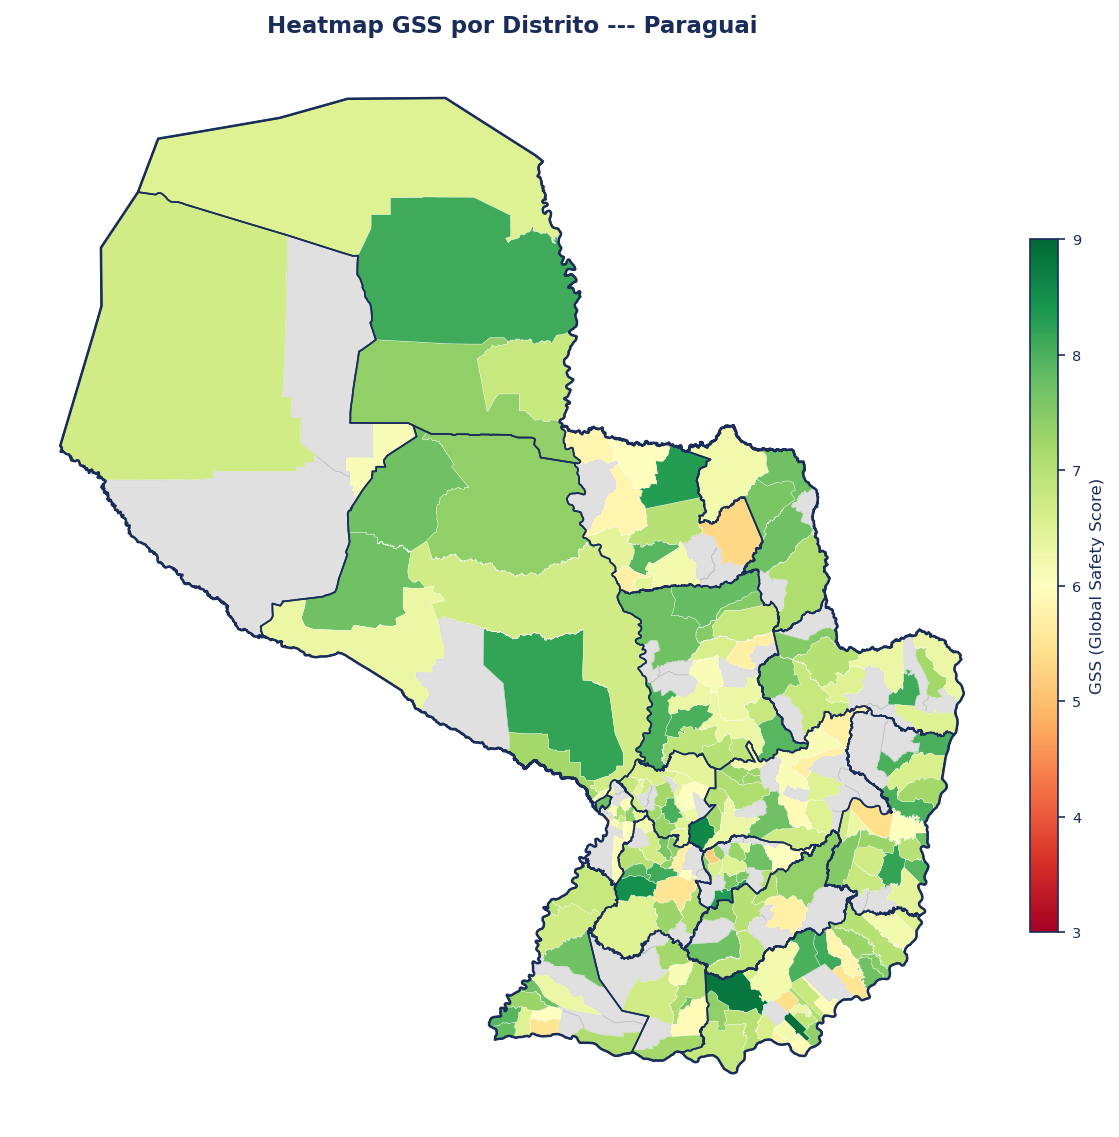
\includegraphics[width=0.82\textwidth, height=0.75\textheight, keepaspectratio]{mapas/heatmap_gss_distrito.pdf}
\caption{Heatmap GSS por Distrito --- Paraguai. Fonte: análise deste guia (2024).}
\label{fig:heatmap-gss-distrito}
\end{figure}

\clearpage

\subsection*{Heatmap GSS Médio por Departamento}

Versão agregada por departamento, com o valor médio do GSS de todos os distritos analisados. Os números dentro de cada departamento indicam o GSS médio.

\begin{figure}[h!]
\centering
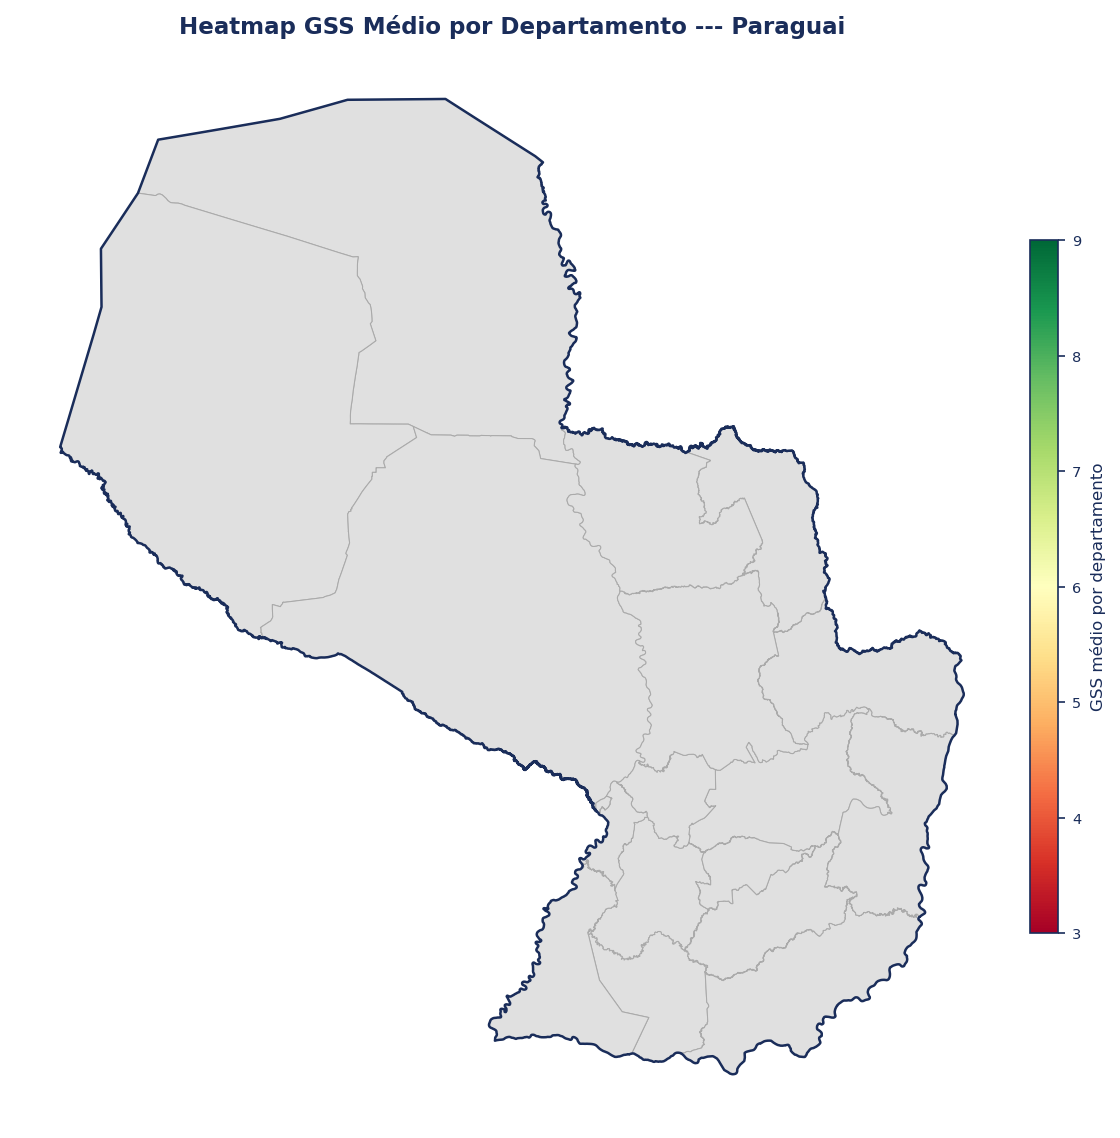
\includegraphics[width=0.82\textwidth, height=0.75\textheight, keepaspectratio]{mapas/heatmap_gss_departamento.pdf}
\caption{GSS Médio por Departamento --- Paraguai. Fonte: análise deste guia (2024).}
\label{fig:heatmap-gss-dept}
\end{figure}

\clearpage

\subsection*{Índice de Desenvolvimento Humano (IDH) por Departamento}

IDH estimado para cada departamento, baseado no relatório PNUD 2020 e dados do Global Data Lab. A escala vai de 0,619 (Alto Paraguay, mais baixo) a 0,835 (Asunción, mais alto).

\begin{figure}[h!]
\centering
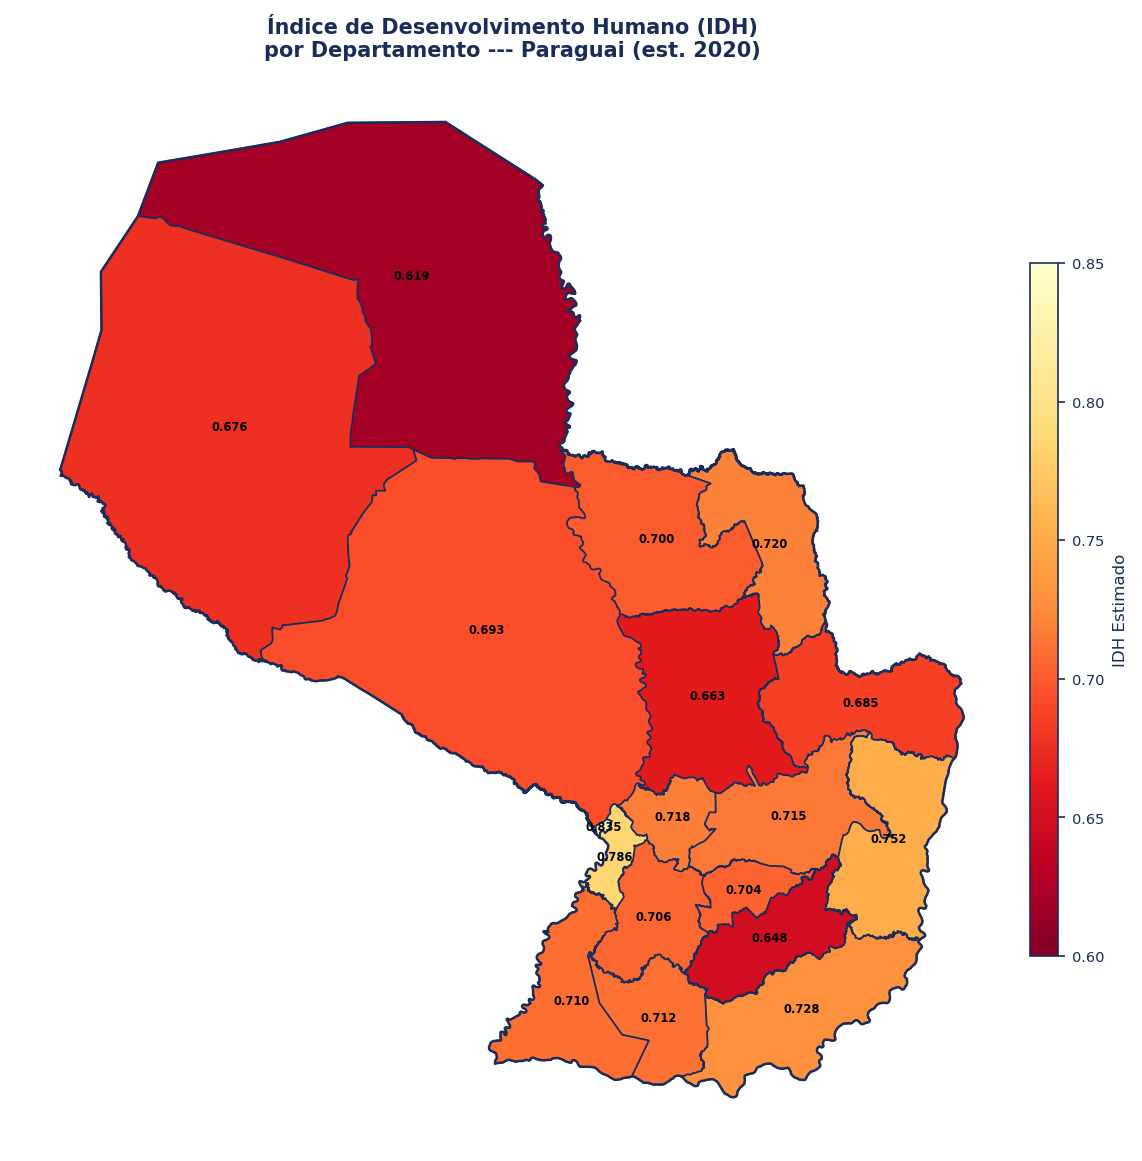
\includegraphics[width=0.82\textwidth, height=0.75\textheight, keepaspectratio]{mapas/mapa_idh_departamento.pdf}
\caption{IDH Estimado por Departamento --- Paraguai. Fonte: PNUD 2020, Global Data Lab.}
\label{fig:mapa-idh}
\end{figure}

\clearpage

\subsection*{Risco Social por Distrito}

Mapa derivado do sub-critério B do GSS (Densidade Populacional e Risco Social). Regiões mais escuras indicam maior risco social --- criminalidade, instabilidade e exposição a fluxo de refugiados em cenários de crise.

\begin{figure}[h!]
\centering
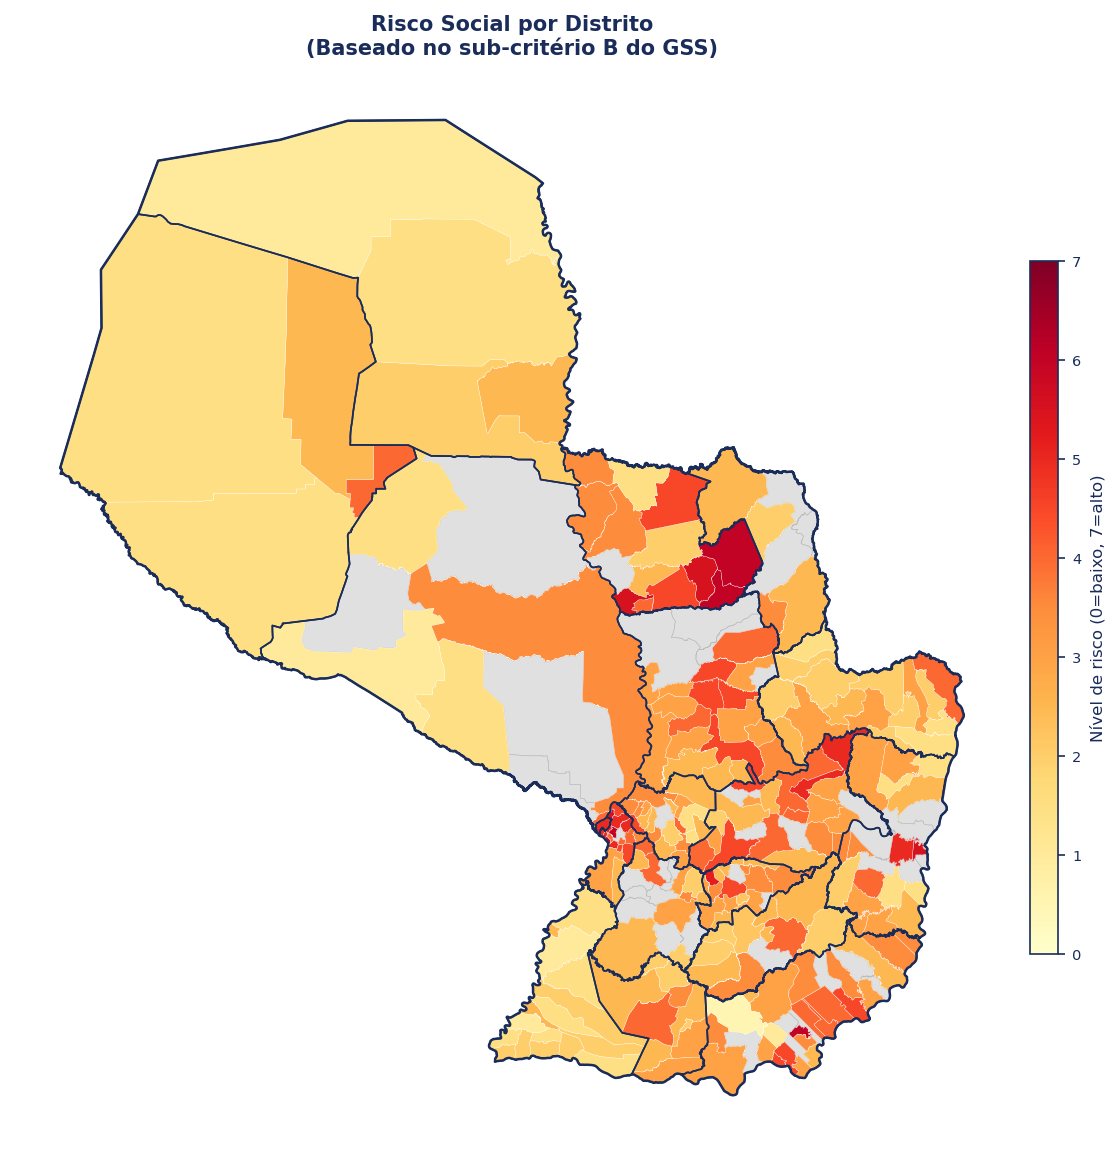
\includegraphics[width=0.82\textwidth, height=0.75\textheight, keepaspectratio]{mapas/mapa_risco_social.pdf}
\caption{Risco Social por Distrito --- Paraguai. Baseado no sub-critério B do GSS (2024).}
\label{fig:mapa-risco}
\end{figure}

\clearpage

\subsection*{Potencial de Autossuficiência por Distrito}

Mapa derivado do sub-critério D do GSS (Solo, Água e Energia). Regiões mais verdes têm maior potencial de autossuficiência alimentar, hídrica e energética.

\begin{figure}[h!]
\centering
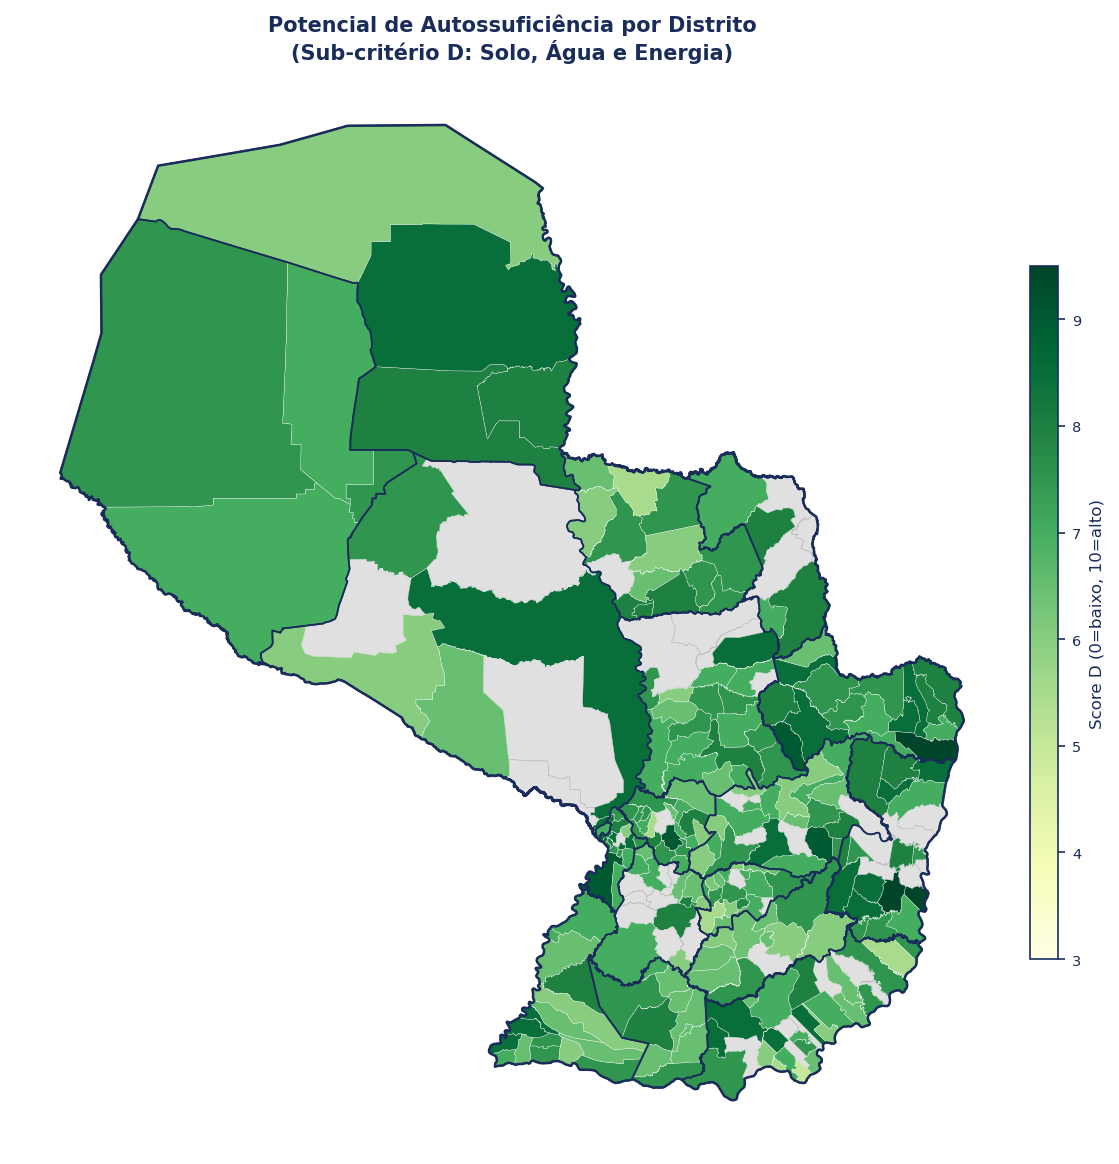
\includegraphics[width=0.82\textwidth, height=0.75\textheight, keepaspectratio]{mapas/mapa_autossuficiencia.pdf}
\caption{Potencial de Autossuficiência por Distrito --- Paraguai. Sub-critério D do GSS (2024).}
\label{fig:mapa-autosuf}
\end{figure}

\clearpage

\subsection*{Irradiação Solar por Departamento}

Média anual de irradiação solar global horizontal (GHI) por departamento, em kWh/m²/dia. Dados da NASA POWER (2001--2020) para a capital de cada departamento. O Chaco Boreal (Boquerón, Alto Paraguay, Presidente Hayes) registra os valores mais altos, com até 5,78 kWh/m²/dia em Filadelfia.

\begin{figure}[h!]
\centering
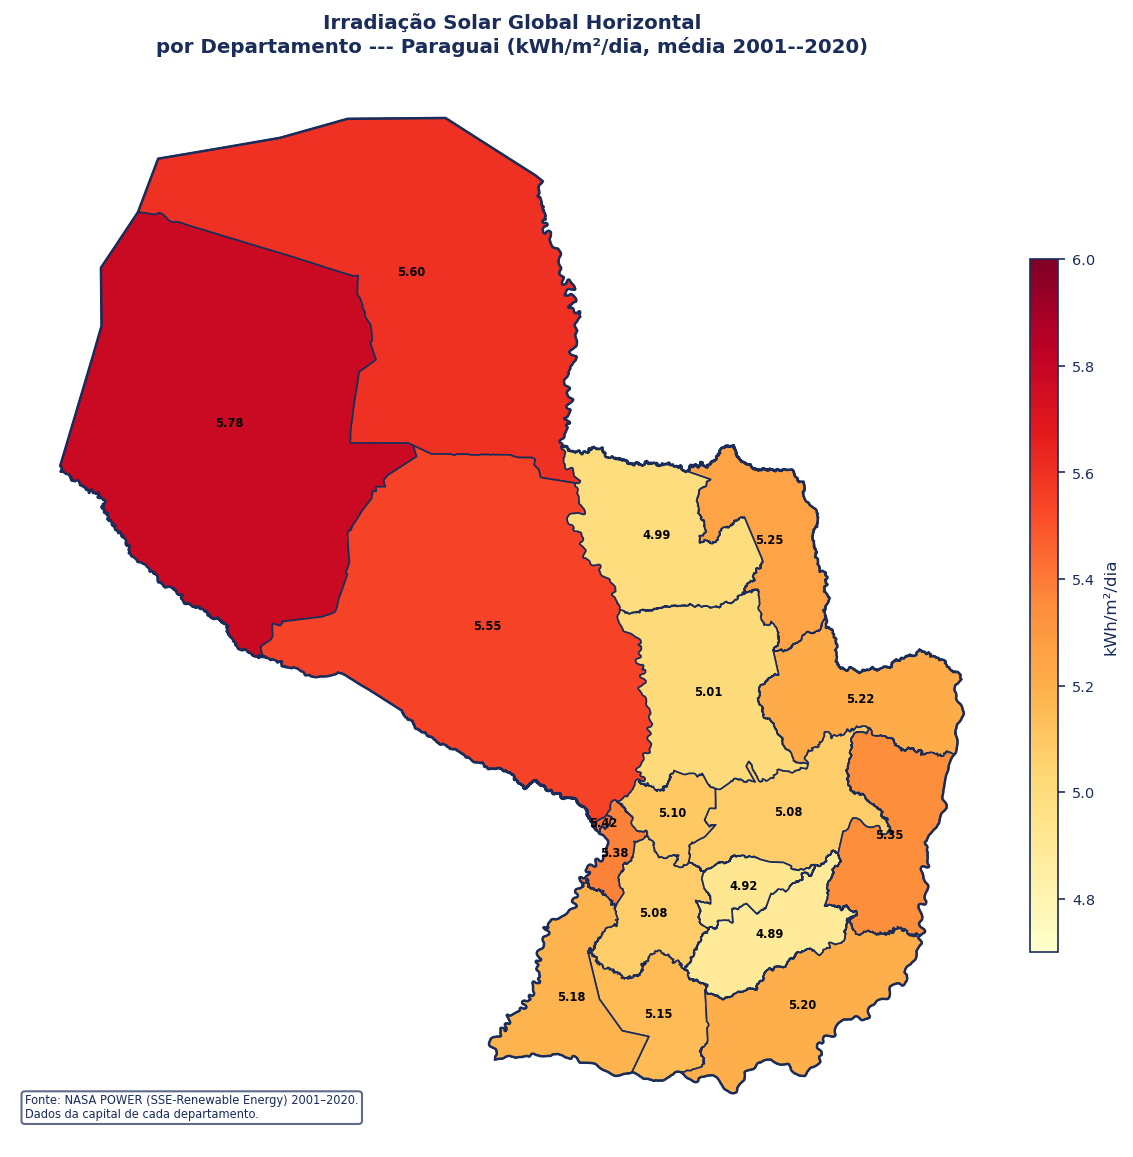
\includegraphics[width=0.82\textwidth, height=0.75\textheight, keepaspectratio]{mapas/mapa_solar_departamento.pdf}
\caption{Irradiação Solar Global Horizontal por Departamento. Fonte: NASA POWER 2001--2020.}
\label{fig:mapa-solar}
\end{figure}

\clearpage

\subsection*{Risco de Inundação por Departamento}

Avaliação qualitativa do risco de inundação sazonal por departamento, baseada em dados da Secretaría de Emergencia Nacional (SEN), DINAC e relatórios da SEAM. Ñeembucú é o departamento com maior risco (planície permanentemente inundável no período de chuvas). Presidente Hayes e Alto Paraguay têm alto risco no Chaco. A Região Oriental tem risco predominantemente baixo a moderado.

\begin{figure}[h!]
\centering
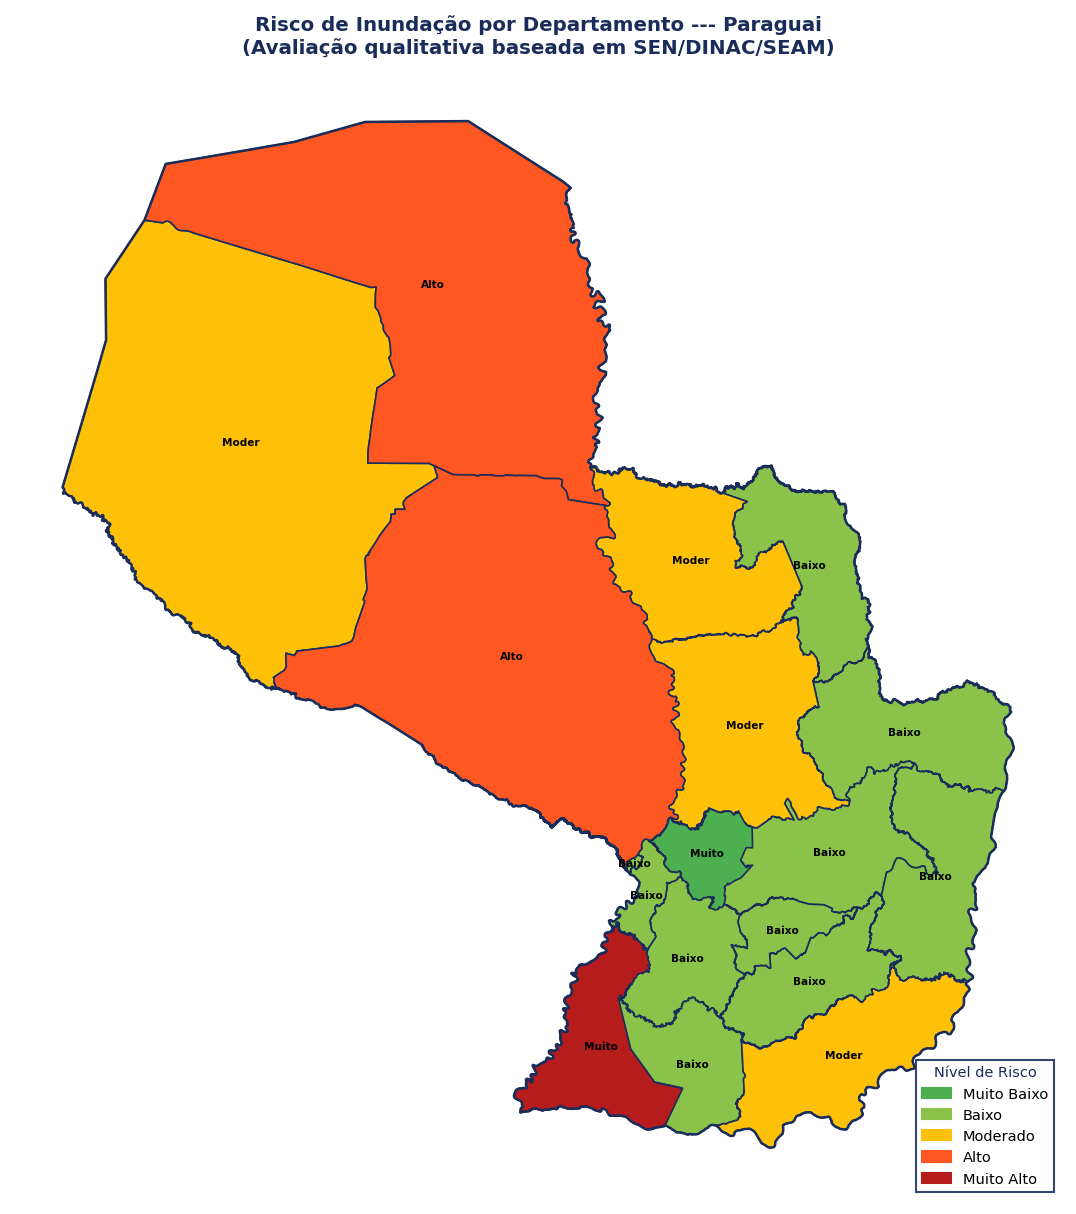
\includegraphics[width=0.82\textwidth, height=0.75\textheight, keepaspectratio]{mapas/mapa_risco_inundacao.pdf}
\caption{Risco de Inundação por Departamento --- Paraguai. Fonte: SEN/DINAC/SEAM, avaliação qualitativa 2024.}
\label{fig:mapa-inundacao}
\end{figure}

\clearpage


\part{Análise por Departamento}
% Lista de departamentos
\chapter{Distrito Capital}\label{dept:Distrito Capital}
\mapaparaguai{0}{Distrito Capital}
\vfill\clearpage
\section{Pacote 02: Distrito Capital /\allowbreak 
Asuncion}

\subsection{Leitura executiva}

Distrito Capital funciona como o nó administrativo, portuário e
institucional do país. Para um leitor que busca autossuficiência ou
preparação, o interesse do distrito não está em terra rural, mas em
acesso a serviços, governança, logística, saúde de alta complexidade e
rede de conexões nacionais.

O pacote 02 consolidou uma leitura em seis eixos:

\begin{itemize}
\tightlist
\item
  estrutura urbana e portuária
\item
  energia e tarifas
\item
  saúde, ensino superior e segurança
\item
  mobilidade e corredores logísticos
\item
  vigilância e capacidade institucional
\item
  lacunas operacionais que exigem cautela analítica
\end{itemize}

\subsection{O que o pacote confirma}

\begin{itemize}
\tightlist
\item
  Asunción reúne o principal porto nacional e a administração portuária
  da ANNP, reforçando o papel do Distrito Capital como nó logístico e
  institucional.
\item
  O recorte demográfico e territorial do distrito está disponível no INE
  via Censo 2022, mas as planilhas detalhadas de população ainda não
  foram extraídas neste ciclo.
\item
  A oferta energética é nacional e operada pela ANDE\footnote{Administración Nacional de Electricidade (Administração Nacional de Eletricidade), companhia estatal de energia.}; a referência
  tarifária consolidada no pacote é o Pliego de Tarifas Nro 21, versão
  atualizada de 27-11-2024, já lida para BT/\allowbreak MT no material de apoio.
\item
  A área metropolitana concentra hospitais especializados de alta
  complexidade, incluindo IMT, INCAN, INE\footnote{Instituto Nacional de Estadística (Instituto Nacional de Estatística), órgão oficial de dados demográficos e censitários.}RAM, Hospital General Barrio
  Obrero, Hospital del Trauma, Hospital Materno Infantil San Pablo,
  Hospital Materno Infantil Santísima Trinidad, Hospital Materno
  Infantil Loma Pyta, Hospital Psiquiátrico e Hospital del Indígena.
\item
  O sistema universitário habilitado inclui instituições como
  Universidad Americana, Universidad Autónoma de Asunción e Universidad
  Adventista del Paraguay, entre outras listadas pelo CONES.
\item
  A capital concentra estruturas penitenciárias de referência, com
  destaque para Tacumbú e a transição institucional do Buen Pastor.
\item
  A malha de segurança passa pelo sistema 911, com monitoramento e
  integração de câmeras urbanas em Asunción.
\item
  A conectividade logística da área metropolitana inclui o Aeroporto
  Internacional Silvio Pettirossi, em Luque, como principal terminal
  aéreo do entorno da capital.
\item
  O serviço postal nacional opera com cobertura em Asunción por meio da
  Dinacopa /\allowbreak  Correos del Paraguay.
\item
  O MIC registrou Asunción como principal polo de novos prestadores
  formais do REPSE no 1º quadrimestre de 2025, reforçando o caráter de
  centro comercial e de serviços do distrito.
\item
  O INE\footnote{Instituto Nacional de Estadística (Instituto Nacional de Estatística), órgão oficial de dados demográficos e censitários.} fechou a projeção populacional de 2025 com 464.185 habitantes,
  mediana de idade de 33 anos, fecundidade de 1,68 filho por mulher e
  anos de estudo médios acima de 11 anos.
\item
  A leitura demográfica e educacional saiu da zona de lacuna aberta e
  entrou na camada de dados consolidados.
\end{itemize}

\subsection{Ficha climática de Assunção (NASA POWER,
2001--2020)}

\textbf{Irradiância solar global --- ALLSKY\_SFC\_SW\_DWN (kWh/\allowbreak m²/\allowbreak dia):}
Jan 6.76 \textbar{} Fev 6.20 \textbar{} Mar 5.42 \textbar{} Abr 4.44
\textbar{} Mai 3.36 \textbar{} Jun 2.83 \textbar{} Jul 3.21 \textbar{}
Ago 3.93 \textbar{} Set 4.61 \textbar{} Out 5.49 \textbar{} Nov 6.42
\textbar{} Dez 6.78 Média anual: 4.95 kWh/\allowbreak m²/\allowbreak dia. Potencial solar
superior à média europeia em todos os meses. Mínimo de inverno (2.83 em
junho) ainda viável para sistemas off-grid.

\textbf{Precipitação --- PRECTOTCORR (mm/\allowbreak dia):} Jan 4.06 \textbar{} Fev
4.92 \textbar{} Mar 4.37 \textbar{} Abr 4.97 \textbar{} Mai 4.62
\textbar{} Jun 2.47 \textbar{} Jul 2.03 \textbar{} Ago 1.23 \textbar{}
Set 2.44 \textbar{} Out 5.27 \textbar{} Nov 6.35 \textbar{} Dez 5.78
Média anual: \textasciitilde1.471 mm/\allowbreak ano. Estação chuvosa Out--Mai;
estação seca Jun--Set. Mínimo em agosto (\textasciitilde38 mm/\allowbreak mês) ---
janela estratégica para obras e instalações externas.

\textbf{Ângulo de inclinação para painéis solares:} 25° ao Norte
(anual); 35° no inverno (Jun--Ago); 15° no verão (Nov--Jan). Fonte: NASA
POWER Climatology API (acesso em 2026-03-20).

\subsection{O que ainda falta
consolidar}

\begin{itemize}
\tightlist
\item
  Custo médio formal de moradia e terra por bairro/\allowbreak distrito.
\item
  Base oficial única para postos de combustível, carregamento elétrico,
  gás encanado e inventário comercial.
\item
  IDH e índices sociais padronizados por distrito.
\item
  Índice de violência por 100 mil habitantes em fonte oficial aberta.
\item
  Poluição luminosa: requer proxy satelital (NOAA/\allowbreak VIIRS).
\end{itemize}

\subsection{Síntese editorial}

Asunción não aparece aqui como ``destino de fuga'', mas como
infraestrutura de apoio. Ela importa porque concentra o que um projeto
no interior precisa quando houver dependência de governo, saúde,
educação, carga regulatória ou tráfego internacional.
\clearpage
\newpage
\secaoDiagnostico{Asuncion}{\mapaConteudo{-25.2666}{-57.6333}}{Asunción é uma capital segura para os padrões globais, mas sofre dos
riscos inerentes a qualquer centro de comando nacional: centralização de
alvos e dependência de redes. Ao mesmo tempo, concentra o porto
nacional, a administração pública, hospitais de alta complexidade,
universidades, o sistema 911, o Aeroporto Silvio Pettirossi e a maior
densidade de serviços do país, o que a torna um polo de apoio e não um
destino autônomo.

\subsubsection{Por que sim}

\begin{itemize}
\tightlist
\item
  Melhor infraestrutura de saúde e serviços do país.
\item
  Estabilidade geológica e segurança institucional.
\item
  Rede logística, energética e regulatória mais completa do Paraguai.
\end{itemize}

\subsubsection{Por que não}

\begin{itemize}
\tightlist
\item
  Concentração de alvos militares e governamentais.
\item
  Densidade populacional elevada.
\item
  Alta dependência de infraestrutura centralizada (energia, água,
  logística).
\end{itemize}

\subsubsection{Recomendação
Técnica}

Ideal como base logística e administrativa, desde que combinada com um
refúgio de nível superior em departamentos mais remotos (como Cordillera
ou Itapúa). Referencia atual de score: GSS 6.5 em 2026-03-05. A leitura
do pacote confirma uma capital funcional para comando, saúde e
conectividade, mas não uma base de autossuficiência plena.

\subsubsection{}

\begin{itemize}
\tightlist
\item
  \begin{enumerate}
  \def\labelenumi{\arabic{enumi})}
  \tightlist
  \item
    Dados censitários validados (INE\footnote{Instituto Nacional de Estadística (Instituto Nacional de Estatística), órgão oficial de dados demográficos e censitários.} 2022).
  \end{enumerate}
\item
  \begin{enumerate}
  \def\labelenumi{\arabic{enumi})}
  \setcounter{enumi}{1}
  \tightlist
  \item
    Indicadores de segurança (Ministerio del Interior 2025).
  \end{enumerate}
\item
  \begin{enumerate}
  \def\labelenumi{\arabic{enumi})}
  \setcounter{enumi}{2}
  \tightlist
  \item
    Mapas de inundação e clima (DMH/\allowbreak SEN\footnote{Secretaría de Emergencia Nacional (Secretaria de Emergência Nacional), órgão governamental de resposta a desastres.} 2026).
  \end{enumerate}
\item
  \begin{enumerate}
  \def\labelenumi{\arabic{enumi})}
  \setcounter{enumi}{3}
  \tightlist
  \item
    Tarifário e infraestrutura energética (ANDE\footnote{Administración Nacional de Electricidade (Administração Nacional de Eletricidade), companhia estatal de energia.} 2026).
  \end{enumerate}
\end{itemize}}
\begin{table}[ht!]
\small \begin{tabular}{p{3.0cm}p{0.8cm}p{6.0cm}} \toprule
\textbf{Critério} & \textbf{Nota} & \textbf{Justificativa} \\ \midrule
A - Ameaças Estratégicas & 5.0 & Capital nacional; alvos militares e governamentais presentes \\
B - Risco Social & 5.0 & Alta densidade metropolitana; risco de convergência de refugiados \\
C - Riscos Naturais & 7.5 & Geologia estável; vulnerabilidade hídrica em áreas específicas \\
D - Autossuficiência & 7.0 & Abundância nacional de energia e água; solo fértil periférico \\
E - Institucional & 8.5 & Forte segurança institucional; baixa taxa de criminalidade violenta \\
\midrule \textbf{GSS FINAL} & \textbf{6.5} & \textbf{Moderadamente Seguro (Recomendado para centros de operação com apoio rural).} \\ \bottomrule \end{tabular}
\end{table}
\subsubsection{Vulnerabilidades e
Mitigação}\label{vuln-Asuncion-vulnerabilidades-e-mitigauxe7uxe3o}

\begin{itemize}
\tightlist
\item
  \textbf{Centralização Política:} Alvo óbvio em crises institucionais
  ou conflitos (Mitigação: manter residência secundária em zona
  rural/\allowbreak periférica).
\item
  \textbf{Dependência de Serviços:} Colapso de rede elétrica ou água
  atinge o núcleo urbano rapidamente (Mitigação: geradores solares e
  cisternas).
\item
  \textbf{Risco de Inundação:} Evitar áreas de baixa cota próximas ao
  rio.
\item
  \textbf{Agitação Social:} Centro de manifestações nacionais
  (Mitigação: localização fora do eixo central/\allowbreak administrativo).
\end{itemize}
\subsubsection{Dossiê de Campo}\label{dossie-Asuncion-dossiuxea-de-campo}
\begin{description}[style=nextline,leftmargin=0.5cm,font=\bfseries]
\item[Coordenadas]  25°16'S 57°38'W.
\item[Topografia]  Colinas suaves (geologicamente estável, risco sísmico desprezível). Margeada pelo Rio Paraguai.
\item[Alvos Estratégicos]  Palácio de los López (Governo), Porto Sajonia (Marinha), Base Ñu Guasu (Aeronáutica/\allowbreak Exército), Aeroporto Silvio Pettirossi (Luque), Hub elétrico de transmissão de Itaipu.
\item[Fallout]  Ventos predominantes: Nordeste (verão - Sirocco, quente) e Sul (inverno - Pampero, frio). Baixo risco de fallout global, mas vulnerável se houver ataques a centros de comando nacionais.
\item[Mapa e media local]  conjunto visual de apoio disponível em `MEDIA.md`, com midia institucional local para uso offline e verificação territorial.
\item[População]  464.185 em 2025 (INE\footnote{Instituto Nacional de Estadística (Instituto Nacional de Estatística), órgão oficial de dados demográficos e censitários.}). Censo 2022 Final: 462.241. Área metropolitana (Gran Asunción) com \textasciitilde 2.200.000.
\item[Densidade]  \textasciitilde 3.950 hab/\allowbreak km² (Núcleo urbano denso).
\item[Vias de Acesso]  Hub central do país. Rutas PY01, PY02, PY03. Gargalos em pontes sobre o Rio Paraguai (Remanso, Héroes del Chaco).
\item[Serviços]  Melhor infraestrutura hospitalar e educacional do país. Investimentos maciços em novos centros de saúde.
\item[Custo de Vida]  US\$ 600-1.550/\allowbreak mês (dependendo do padrão). Terrenos urbanos: US\$ 400-650/\allowbreak m².
\item[Saúde de alta complexidade]  IMT, INCAN, INE\footnote{Instituto Nacional de Estadística (Instituto Nacional de Estatística), órgão oficial de dados demográficos e censitários.}RAM, Hospital General Barrio Obrero, Hospital del Trauma, Hospital Materno Infantil San Pablo, Hospital Materno Infantil Santísima Trinidad, Hospital Materno Infantil Loma Pyta, Hospital Psiquiátrico e Hospital del Indígena concentram oferta especializada na capital.
\item[Universidades habilitadas]  Asunción concentra oferta do CONES, com instituições como Universidad Americana, Universidad Autónoma de Asunción e Universidad Adventista del Paraguay.
\item[Conexões logísticas]  Porto de Asunción, sistema 911 e Aeroporto Internacional Silvio Pettirossi reforçam a função de nó administrativo, portuário e metropolitano.
\item[Idade mediana]  33 anos em 2025, segundo projeções do INE\footnote{Instituto Nacional de Estadística (Instituto Nacional de Estatística), órgão oficial de dados demográficos e censitários.}.
\item[Fecundidade]  1,64 filho por mulher em 2022 e 1,68 em 2025 nas projeções do INE\footnote{Instituto Nacional de Estadística (Instituto Nacional de Estatística), órgão oficial de dados demográficos e censitários.}.
\item[Escolaridade]  11,7 anos de estudo em homens e 11,4 em mulheres na faixa de 15+ anos; a cidade concentra o maior capital educacional do país.
\item[Assistência escolar]  os indicadores nacionais da EPHC 2025 mostram 39,4\% de frequência geral e 97,7\% de assistência entre 5 e 9 anos.
\item[Hidrologia]  Risco de Inundação Recorrente. Áreas ribeirinhas (Bañados) sofrem cheias periódicas ligadas ao El Niño.
\item[Clima]  Tropical/\allowbreak Subtropical. Verões com temperaturas >40°C. Tempestades severas com rajadas de vento de até 160 km/\allowbreak h.
\item[Sismicidade]  Muito baixa. Região tectonicamente estável.
\item[Irradiância solar global — ALLSKY\_SFC\_SW\_DWN (kWh/\allowbreak m²/\allowbreak dia)]  Jan 6.76 | Fev 6.20 | Mar 5.42 | Abr 4.44 | Mai 3.36 | Jun 2.83 | Jul 3.21 | Ago 3.93 | Set 4.61 | Out 5.49 | Nov 6.42 | Dez 6.78. Média anual: 4.95 kWh/\allowbreak m²/\allowbreak dia. Mínimo: Jun (2.83) | Máximo: Dez (6.78). Fonte: NASA POWER Climatology API, período 2001-2020 (acesso em 2026-03-20).
\item[Precipitação — PRECTOTCORR (mm/\allowbreak mês)]  Jan 4.06 | Fev 4.92 | Mar 4.37 | Abr 4.97 | Mai 4.62 | Jun 2.47 | Jul 2.03 | Ago 1.23 | Set 2.44 | Out 5.27 | Nov 6.35 | Dez 5.78. Média anual: \textasciitilde 1.471 mm/\allowbreak ano. Estação chuvosa Out-Mai; seca Jun-Set (mínimo em Ago). Fonte: NASA POWER (acesso em 2026-03-20).
\item[Inclinação recomendada para placas solares]  25° voltado para o Norte (anual); 35° no inverno (Jun-Ago); 15° no verão (Nov-Jan). Base: latitude local -25.28°S.
\item[Energia]  Dependência total da rede nacional (Itaipu), mas com a energia mais barata da região (\textasciitilde US\$ 0,05/\allowbreak kWh).
\item[Água]  Abundante (Rio Paraguai), tratamento centralizado pela ESSAP\footnote{Empresa de Servicios Sanitarios del Paraguay (Empresa de Serviços Sanitários do Paraguai), responsável pelo saneamento e água urbana.}.
\item[Solo]  Solo fértil na Região Oriental, mas área urbana saturada. Potencial agrícola nos arredores (Central/\allowbreak Chaco'i).
\item[Autossuficiência]  Baixa no núcleo urbano; alta dependência de suprimentos logísticos nacionais e internacionais.
\item[Internet de alta velocidade]  110 pontos de WiFi libre foram habilitados em Asunción pelo MITIC; 320 novos pontos chegaram ao país em 2023, com cobertura nacional ampliada.
\item[Rede celular]  a tecnologia 5G foi lançada oficialmente no país em dezembro de 2025 e teve ato em Asunción, no Paseo La Galería.
\item[Poços e águas subterrâneas]  não há profundidade média oficial consolidada para poços artesianos em Asunción; a regulação permanece com MADES e Lei 3239/\allowbreak 07.
\item[Combustível e gás]  não foi identificado inventário oficial único por distrito para postos, eletropostos e distribuição de gás encanado.
\item[Serviço público digital]  a municipalidade de Asunción iniciou processo de transformação digital com apoio do MITIC em 2025.
\item[Segurança]  Taxa de homicídios baixa para padrões latinos (7.1/\allowbreak 100k). Criminalidade focada em delitos contra o patrimônio. Áreas nobres e corporativas são consideradas seguras.
\item[Leis Local]  Sede do governo central. Direitos de propriedade bem definidos. Incentivos fiscais (Lei 60/\allowbreak 90).
\item[Delegacias]  Dirección de Policía de Asunción com 23 comisarías jurisdicionais listadas pela Policía Nacional.
\item[Presídios]  Tacumbú concentra 2.151 PPL em censo recente do Ministério de Justicia; o conjunto penitenciário de Asunción também inclui UPIE e Granja Ko'e Pyahu, com mais de 2.200 PPL em visita institucional de 2025.
\item[Correios e entregas]  Correos del Paraguay opera cobertura nacional e atende a capital; não há tabela oficial única de desempenho local por bairro.
\item[Comércio urbano]  o MIC publicou o REPSE do 1º quadrimestre de 2025 com Asunción concentrando 32,2\% dos novos prestadores de serviços do país, o que funciona como proxy oficial de dinamismo comercial formal; o inventário centralizado de cinemas, shoppings e atacados segue sem tabela única.
\item[Escolaridade e ensino superior]  INE\footnote{Instituto Nacional de Estadística (Instituto Nacional de Estatística), órgão oficial de dados demográficos e censitários.} e CONES são as bases centrais para alfabetização, escolaridade e oferta universitária; a extração fina por recorte territorial permanece parcial.
\item[Demografia social]  idade mediana de 33 anos e fecundidade de 1,68 filho por mulher em 2025; o item já saiu da zona de lacuna aberta.
\item[Poluição luminosa]  Bortle 8 (céu urbano), radiância artificial estimada em 100 nW/\allowbreak cm²/\allowbreak sr. Fonte: World Atlas of Artificial Night Sky Brightness.
\end{description}
\paragraph{Solo (SoilGrids 2.0, média ponderada 0--30
cm)}

\begin{longtable}[]{@{}ll@{}}
\toprule\noalign{}
Parâmetro & Valor \\
\midrule\noalign{}
\endhead
\bottomrule\noalign{}
\endlastfoot
pH (H$_2$O) & 5.72 \\
Carbono orgânico (SOC) & 24.33 g/\allowbreak kg \\
Argila & 19.82 \% \\
Areia & 56.72 \% \\
Silte (calc.) & 23.5 \% \\
Densidade aparente & 1.21 g/\allowbreak cm³ \\
\textbf{Aptidão agrícola} & \textbf{Alta} \\
\end{longtable}

Fonte: ISRIC SoilGrids 2.0 via WCS (acesso em 2026-03-21). Coords:
-25.2667°, -57.6333°. Média ponderada camadas 0-5, 5-15, 15-30 cm.

\begin{itemize}
\tightlist
\item
  \textbf{Autossuficiência:} Baixa no núcleo urbano; alta dependência de
  suprimentos logísticos nacionais e internacionais.
\item
  \textbf{Internet de alta velocidade:} 110 pontos de WiFi libre foram
  habilitados em Asunción pelo MITIC; 320 novos pontos chegaram ao país
  em 2023, com cobertura nacional ampliada.
\item
  \textbf{Rede celular:} a tecnologia 5G foi lançada oficialmente no
  país em dezembro de 2025 e teve ato em Asunción, no Paseo La Galería.
\item
  \textbf{Poços e águas subterrâneas:} não há profundidade média oficial
  consolidada para poços artesianos em Asunción; a regulação permanece
  com MADES e Lei 3239/\allowbreak 07.
\item
  \textbf{Combustível e gás:} não foi identificado inventário oficial
  único por distrito para postos, eletropostos e distribuição de gás
  encanado.
\item
  \textbf{Serviço público digital:} a municipalidade de Asunción iniciou
  processo de transformação digital com apoio do MITIC em 2025.
\end{itemize}

\chapter{Concepción}\label{dept:Concepción}
\mapaparaguai{1}{Concepción}
\vfill\clearpage
\section{Concepción}

\subsection{Ficha climática de Concepción (capital
departamental)}

\textbf{Irradiância solar global --- (kWh/\allowbreak m²/\allowbreak dia):}

{\def\LTcaptype{none} % do not increment counter
\begin{longtable}[]{@{}
  >{\raggedright\arraybackslash}p{(\linewidth - 22\tabcolsep) * \real{0.0833}}
  >{\raggedright\arraybackslash}p{(\linewidth - 22\tabcolsep) * \real{0.0833}}
  >{\raggedright\arraybackslash}p{(\linewidth - 22\tabcolsep) * \real{0.0833}}
  >{\raggedright\arraybackslash}p{(\linewidth - 22\tabcolsep) * \real{0.0833}}
  >{\raggedright\arraybackslash}p{(\linewidth - 22\tabcolsep) * \real{0.0833}}
  >{\raggedright\arraybackslash}p{(\linewidth - 22\tabcolsep) * \real{0.0833}}
  >{\raggedright\arraybackslash}p{(\linewidth - 22\tabcolsep) * \real{0.0833}}
  >{\raggedright\arraybackslash}p{(\linewidth - 22\tabcolsep) * \real{0.0833}}
  >{\raggedright\arraybackslash}p{(\linewidth - 22\tabcolsep) * \real{0.0833}}
  >{\raggedright\arraybackslash}p{(\linewidth - 22\tabcolsep) * \real{0.0833}}
  >{\raggedright\arraybackslash}p{(\linewidth - 22\tabcolsep) * \real{0.0833}}
  >{\raggedright\arraybackslash}p{(\linewidth - 22\tabcolsep) * \real{0.0833}}@{}}
\toprule\noalign{}
\begin{minipage}[b]{\linewidth}\raggedright
Jan
\end{minipage} & \begin{minipage}[b]{\linewidth}\raggedright
Fev
\end{minipage} & \begin{minipage}[b]{\linewidth}\raggedright
Mar
\end{minipage} & \begin{minipage}[b]{\linewidth}\raggedright
Abr
\end{minipage} & \begin{minipage}[b]{\linewidth}\raggedright
Mai
\end{minipage} & \begin{minipage}[b]{\linewidth}\raggedright
Jun
\end{minipage} & \begin{minipage}[b]{\linewidth}\raggedright
Jul
\end{minipage} & \begin{minipage}[b]{\linewidth}\raggedright
Ago
\end{minipage} & \begin{minipage}[b]{\linewidth}\raggedright
Set
\end{minipage} & \begin{minipage}[b]{\linewidth}\raggedright
Out
\end{minipage} & \begin{minipage}[b]{\linewidth}\raggedright
Nov
\end{minipage} & \begin{minipage}[b]{\linewidth}\raggedright
Dez
\end{minipage} \\
\midrule\noalign{}
\endhead
\bottomrule\noalign{}
\endlastfoot
6.68 & 6.07 & 5.58 & 4.63 & 3.47 & 3.00 & 3.30 & 4.09 & 4.68 & 5.49 &
6.34 & 6.61 \\
\end{longtable}
}

Média anual: 4.99 kWh/\allowbreak m²/\allowbreak dia. Inclinação recomendada: 23° Norte (anual);
33° inverno; 13° verão.

\textbf{Precipitação --- (mm/\allowbreak mês):}

{\def\LTcaptype{none} % do not increment counter
\begin{longtable}[]{@{}
  >{\raggedright\arraybackslash}p{(\linewidth - 22\tabcolsep) * \real{0.0833}}
  >{\raggedright\arraybackslash}p{(\linewidth - 22\tabcolsep) * \real{0.0833}}
  >{\raggedright\arraybackslash}p{(\linewidth - 22\tabcolsep) * \real{0.0833}}
  >{\raggedright\arraybackslash}p{(\linewidth - 22\tabcolsep) * \real{0.0833}}
  >{\raggedright\arraybackslash}p{(\linewidth - 22\tabcolsep) * \real{0.0833}}
  >{\raggedright\arraybackslash}p{(\linewidth - 22\tabcolsep) * \real{0.0833}}
  >{\raggedright\arraybackslash}p{(\linewidth - 22\tabcolsep) * \real{0.0833}}
  >{\raggedright\arraybackslash}p{(\linewidth - 22\tabcolsep) * \real{0.0833}}
  >{\raggedright\arraybackslash}p{(\linewidth - 22\tabcolsep) * \real{0.0833}}
  >{\raggedright\arraybackslash}p{(\linewidth - 22\tabcolsep) * \real{0.0833}}
  >{\raggedright\arraybackslash}p{(\linewidth - 22\tabcolsep) * \real{0.0833}}
  >{\raggedright\arraybackslash}p{(\linewidth - 22\tabcolsep) * \real{0.0833}}@{}}
\toprule\noalign{}
\begin{minipage}[b]{\linewidth}\raggedright
Jan
\end{minipage} & \begin{minipage}[b]{\linewidth}\raggedright
Fev
\end{minipage} & \begin{minipage}[b]{\linewidth}\raggedright
Mar
\end{minipage} & \begin{minipage}[b]{\linewidth}\raggedright
Abr
\end{minipage} & \begin{minipage}[b]{\linewidth}\raggedright
Mai
\end{minipage} & \begin{minipage}[b]{\linewidth}\raggedright
Jun
\end{minipage} & \begin{minipage}[b]{\linewidth}\raggedright
Jul
\end{minipage} & \begin{minipage}[b]{\linewidth}\raggedright
Ago
\end{minipage} & \begin{minipage}[b]{\linewidth}\raggedright
Set
\end{minipage} & \begin{minipage}[b]{\linewidth}\raggedright
Out
\end{minipage} & \begin{minipage}[b]{\linewidth}\raggedright
Nov
\end{minipage} & \begin{minipage}[b]{\linewidth}\raggedright
Dez
\end{minipage} \\
\midrule\noalign{}
\endhead
\bottomrule\noalign{}
\endlastfoot
157 & 151 & 120 & 139 & 116 & 71 & 48 & 31 & 73 & 151 & 204 & 167 \\
\end{longtable}
}

Média anual: \textasciitilde1.427 mm/\allowbreak ano. Estação chuvosa Out-Mai; seca
Jun-Set.
\clearpage
\subsection*{Dados Departamentais}
\subsubsection{Desenvolvimento Humano e
Social}

\subsection{IDH Departamental}

{\def\LTcaptype{none} % do not increment counter
\begin{longtable}[]{@{}ll@{}}
\toprule\noalign{}
Indicador & Valor \\
\midrule\noalign{}
\endhead
\bottomrule\noalign{}
\endlastfoot
IDH & 0,700 \\
Classificação IDH & alto \\
Ranking nacional (1=melhor) & 9/\allowbreak 18 \\
Esperança de vida & 72,4 anos \\
Anos de escolaridade média & 8,1 anos \\
RNB per capita (USD PPA) & 8.400 \\
\end{longtable}
}

\subsection{Indicadores de Pobreza}

{\def\LTcaptype{none} % do not increment counter
\begin{longtable}[]{@{}ll@{}}
\toprule\noalign{}
Indicador & Valor \\
\midrule\noalign{}
\endhead
\bottomrule\noalign{}
\endlastfoot
Taxa de pobreza total (\%) & 31,1\% \\
Taxa de pobreza extrema (\%) & 7,8\% \\
Índice de Gini & 0,460 \\
\end{longtable}
}

\subsection{Infraestrutura Básica}

{\def\LTcaptype{none} % do not increment counter
\begin{longtable}[]{@{}ll@{}}
\toprule\noalign{}
Indicador & Valor \\
\midrule\noalign{}
\endhead
\bottomrule\noalign{}
\endlastfoot
Acesso a água potável (\%) & 74,2\% \\
Acesso a saneamento (\%) & 71,8\% \\
\end{longtable}
}

\subsubsection{Segurança Pública}

\subsection{Indicadores}

{\def\LTcaptype{none} % do not increment counter
\begin{longtable}[]{@{}
  >{\raggedright\arraybackslash}p{(\linewidth - 2\tabcolsep) * \real{0.6111}}
  >{\raggedright\arraybackslash}p{(\linewidth - 2\tabcolsep) * \real{0.3889}}@{}}
\toprule\noalign{}
\begin{minipage}[b]{\linewidth}\raggedright
Indicador
\end{minipage} & \begin{minipage}[b]{\linewidth}\raggedright
Valor
\end{minipage} \\
\midrule\noalign{}
\endhead
\bottomrule\noalign{}
\endlastfoot
Taxa de homicídios (por 100k hab) & \textasciitilde12--15 (estimativa,
acima da média nacional) \\
Crimes registrados (total/\allowbreak ano) & --- dados não desagregados
publicamente \\
Número de comisarías & \textasciitilde15 (estimativa departamental) \\
Índice segurança relativo & baixo \\
\end{longtable}
}

\subsubsection{Mercado de Terra Rural}

\subsection{Preços por Tipo de Terra}

{\def\LTcaptype{none} % do not increment counter
\begin{longtable}[]{@{}llll@{}}
\toprule\noalign{}
Tipo & Preço (USD/\allowbreak ha) & Faixa & Tendência \\
\midrule\noalign{}
\endhead
\bottomrule\noalign{}
\endlastfoot
Agrícola alta produtividade & 3.500 & 2.500 -- 5.000 & ↑ \\
Pastagem & 1.800 & 1.200 -- 2.500 & ↑ \\
Mata /\allowbreak  reserva & 600 & 300 -- 1.000 & → \\
\end{longtable}
}

\subsection{Características do
Mercado}

{\def\LTcaptype{none} % do not increment counter
\begin{longtable}[]{@{}
  >{\raggedright\arraybackslash}p{(\linewidth - 2\tabcolsep) * \real{0.6111}}
  >{\raggedright\arraybackslash}p{(\linewidth - 2\tabcolsep) * \real{0.3889}}@{}}
\toprule\noalign{}
\begin{minipage}[b]{\linewidth}\raggedright
Parâmetro
\end{minipage} & \begin{minipage}[b]{\linewidth}\raggedright
Valor
\end{minipage} \\
\midrule\noalign{}
\endhead
\bottomrule\noalign{}
\endlastfoot
Valorização anual média (\%) & 6--8\% \\
Lote mínimo rural (ha) & 20 \\
Imposto territorial rural (\%) & 1\% sobre valor fiscal (IRAGRO
adicional para renda) \\
Liquidez do mercado & média \\
\end{longtable}
}
\clearpage
\newpage
\secaoDiagnostico{Arroyito}{\mapaDistrito{0112}}{Arroyito é um distrito de origem camponesa com solo altamente produtivo,
mas marcado pela insegurança regional. Oferece baixo custo de vida e boa
capacidade de produção de alimentos, mas exige um alto nível de
tolerância ao risco devido à presença da insurgência no departamento.

\subsubsection{Por que sim}

\subsubsection{Por que não}

\subsubsection{Recomendação
Técnica}

Indicado para projetos de autossuficiência alimentar que possam ser
integrados à comunidade local e que possuam planos de segurança
robustos. Referência atual de score: GSS 5.5.

\begin{itemize}
\tightlist
\item
  \begin{enumerate}
  \def\labelenumi{\arabic{enumi})}
  \tightlist
  \item
    Dados censitários INE\footnote{\fineINE} 2022 (Arroyito Distrito).
  \end{enumerate}
\item
  \begin{enumerate}
  \def\labelenumi{\arabic{enumi})}
  \setcounter{enumi}{1}
  \tightlist
  \item
    Histórico de assentamento camponês (1989-2016).
  \end{enumerate}
\item
  \begin{enumerate}
  \def\labelenumi{\arabic{enumi})}
  \setcounter{enumi}{2}
  \tightlist
  \item
    Relatórios de segurança pública (FTC/\allowbreak CODI).
  \end{enumerate}
\item
  \begin{enumerate}
  \def\labelenumi{\arabic{enumi})}
  \setcounter{enumi}{3}
  \tightlist
  \item
    Lei de Segurança Fronteiriça (2532/\allowbreak 05).
  \end{enumerate}
\end{itemize}}{dist:01_Concepción:Arroyito}
\begin{table}[ht!]
\small \begin{tabular}{p{3.0cm}p{0.8cm}p{6.0cm}} \toprule
\textbf{Critério} & \textbf{Nota} & \textbf{Justificativa} \\ \midrule
A - Ameaças Estratégicas & 3.5 & Hotspot de insurgência regional e presença militar constante \\
B - Risco Social & 4.5 & Assentamento com histórico de agitação social e criminalidade rural \\
C - Riscos Naturais & 7.0 & Baixo risco de desastres geológicos; riscos climáticos manejáveis \\
D - Autossuficiência & 7.5 & Solo fértil e abundância de produção de alimentos básicos \\
E - Institucional & 5.5 & Ambiente institucional em consolidação; fortes restrições de fronteira \\
\midrule \textbf{GSS FINAL} & \textbf{5.5} & \textbf{Moderadamente Seguro (Recomendado apenas para perfis resilientes com foco em agricultura familiar e segurança tática).} \\ \bottomrule \end{tabular}
\end{table}
\subsubsection{Vulnerabilidades e
Mitigação}

\begin{itemize}
\tightlist
\item
  Exposicao hidrometeorologica moderada (45-64/\allowbreak 100).
\item
  Conectividade viaria intermediaria (50-69/\allowbreak 100).
\item
  Estoque de contingencia para 14 dias (agua/\allowbreak alimentos/\allowbreak combustivel),
  priorizado quando risco hidro=50/\allowbreak 100.
\item
  Duplicar rotas/\allowbreak logistica quando conectividade viaria=62/\allowbreak 100 for
  \textless70; manter rota secundaria mapeada e testada trimestralmente.
\item
  Plano de energia resiliente com autonomia minima de 72h
  (geracao/\allowbreak backup), revisao semestral.
\end{itemize}

\subsubsection{Dossiê de Campo}
\begin{description}[style=nextline,leftmargin=0.5cm,font=\bfseries]
\item[Coordenadas]  22°39'S 57°50'W (geocodificado via Nominatim).
\end{description}
\textbf{Fonte climática:} NASA POWER Climatology API (período 2001-2020)

\textbf{Fonte luminosa:} estimativa world atlas

\paragraph{Irradiação Solar
(kWh/\allowbreak m²/\allowbreak dia)}

{\def\LTcaptype{none} % do not increment counter
\begin{longtable}[]{@{}
  >{\raggedright\arraybackslash}p{(\linewidth - 24\tabcolsep) * \real{0.0746}}
  >{\raggedright\arraybackslash}p{(\linewidth - 24\tabcolsep) * \real{0.0746}}
  >{\raggedright\arraybackslash}p{(\linewidth - 24\tabcolsep) * \real{0.0746}}
  >{\raggedright\arraybackslash}p{(\linewidth - 24\tabcolsep) * \real{0.0746}}
  >{\raggedright\arraybackslash}p{(\linewidth - 24\tabcolsep) * \real{0.0746}}
  >{\raggedright\arraybackslash}p{(\linewidth - 24\tabcolsep) * \real{0.0746}}
  >{\raggedright\arraybackslash}p{(\linewidth - 24\tabcolsep) * \real{0.0746}}
  >{\raggedright\arraybackslash}p{(\linewidth - 24\tabcolsep) * \real{0.0746}}
  >{\raggedright\arraybackslash}p{(\linewidth - 24\tabcolsep) * \real{0.0746}}
  >{\raggedright\arraybackslash}p{(\linewidth - 24\tabcolsep) * \real{0.0746}}
  >{\raggedright\arraybackslash}p{(\linewidth - 24\tabcolsep) * \real{0.0746}}
  >{\raggedright\arraybackslash}p{(\linewidth - 24\tabcolsep) * \real{0.0746}}
  >{\raggedright\arraybackslash}p{(\linewidth - 24\tabcolsep) * \real{0.1045}}@{}}
\toprule\noalign{}
\begin{minipage}[b]{\linewidth}\raggedright
Jan
\end{minipage} & \begin{minipage}[b]{\linewidth}\raggedright
Fev
\end{minipage} & \begin{minipage}[b]{\linewidth}\raggedright
Mar
\end{minipage} & \begin{minipage}[b]{\linewidth}\raggedright
Abr
\end{minipage} & \begin{minipage}[b]{\linewidth}\raggedright
Mai
\end{minipage} & \begin{minipage}[b]{\linewidth}\raggedright
Jun
\end{minipage} & \begin{minipage}[b]{\linewidth}\raggedright
Jul
\end{minipage} & \begin{minipage}[b]{\linewidth}\raggedright
Ago
\end{minipage} & \begin{minipage}[b]{\linewidth}\raggedright
Set
\end{minipage} & \begin{minipage}[b]{\linewidth}\raggedright
Out
\end{minipage} & \begin{minipage}[b]{\linewidth}\raggedright
Nov
\end{minipage} & \begin{minipage}[b]{\linewidth}\raggedright
Dez
\end{minipage} & \begin{minipage}[b]{\linewidth}\raggedright
Média
\end{minipage} \\
\midrule\noalign{}
\endhead
\bottomrule\noalign{}
\endlastfoot
6.55 & 5.94 & 5.63 & 4.73 & 3.58 & 3.17 & 3.41 & 4.19 & 4.70 & 5.44 &
6.28 & 6.49 & \textbf{5.01} \\
\end{longtable}
}

\textbf{Inclinação solar recomendada:} 23° N (anual) · 33° N (inverno
jun-ago) · 13° N (verão nov-jan)

\paragraph{Precipitação (mm/\allowbreak mês)}

{\def\LTcaptype{none} % do not increment counter
\begin{longtable}[]{@{}
  >{\raggedright\arraybackslash}p{(\linewidth - 24\tabcolsep) * \real{0.0704}}
  >{\raggedright\arraybackslash}p{(\linewidth - 24\tabcolsep) * \real{0.0704}}
  >{\raggedright\arraybackslash}p{(\linewidth - 24\tabcolsep) * \real{0.0704}}
  >{\raggedright\arraybackslash}p{(\linewidth - 24\tabcolsep) * \real{0.0704}}
  >{\raggedright\arraybackslash}p{(\linewidth - 24\tabcolsep) * \real{0.0704}}
  >{\raggedright\arraybackslash}p{(\linewidth - 24\tabcolsep) * \real{0.0704}}
  >{\raggedright\arraybackslash}p{(\linewidth - 24\tabcolsep) * \real{0.0704}}
  >{\raggedright\arraybackslash}p{(\linewidth - 24\tabcolsep) * \real{0.0704}}
  >{\raggedright\arraybackslash}p{(\linewidth - 24\tabcolsep) * \real{0.0704}}
  >{\raggedright\arraybackslash}p{(\linewidth - 24\tabcolsep) * \real{0.0704}}
  >{\raggedright\arraybackslash}p{(\linewidth - 24\tabcolsep) * \real{0.0704}}
  >{\raggedright\arraybackslash}p{(\linewidth - 24\tabcolsep) * \real{0.0704}}
  >{\raggedright\arraybackslash}p{(\linewidth - 24\tabcolsep) * \real{0.1549}}@{}}
\toprule\noalign{}
\begin{minipage}[b]{\linewidth}\raggedright
Jan
\end{minipage} & \begin{minipage}[b]{\linewidth}\raggedright
Fev
\end{minipage} & \begin{minipage}[b]{\linewidth}\raggedright
Mar
\end{minipage} & \begin{minipage}[b]{\linewidth}\raggedright
Abr
\end{minipage} & \begin{minipage}[b]{\linewidth}\raggedright
Mai
\end{minipage} & \begin{minipage}[b]{\linewidth}\raggedright
Jun
\end{minipage} & \begin{minipage}[b]{\linewidth}\raggedright
Jul
\end{minipage} & \begin{minipage}[b]{\linewidth}\raggedright
Ago
\end{minipage} & \begin{minipage}[b]{\linewidth}\raggedright
Set
\end{minipage} & \begin{minipage}[b]{\linewidth}\raggedright
Out
\end{minipage} & \begin{minipage}[b]{\linewidth}\raggedright
Nov
\end{minipage} & \begin{minipage}[b]{\linewidth}\raggedright
Dez
\end{minipage} & \begin{minipage}[b]{\linewidth}\raggedright
Total/\allowbreak ano
\end{minipage} \\
\midrule\noalign{}
\endhead
\bottomrule\noalign{}
\endlastfoot
152 & 149 & 120 & 118 & 106 & 57 & 38 & 23 & 55 & 130 & 202 & 167 &
\textbf{1321 mm} \\
\end{longtable}
}

\paragraph{Poluição Luminosa}

{\def\LTcaptype{none} % do not increment counter
\begin{longtable}[]{@{}ll@{}}
\toprule\noalign{}
Parâmetro & Valor \\
\midrule\noalign{}
\endhead
\bottomrule\noalign{}
\endlastfoot
Escala Bortle & 2 --- Céu tipicamente escuro \\
Radiância artificial & 0.3 nW/\allowbreak cm²/\allowbreak sr \\
\end{longtable}
}
\paragraph{Solo (SoilGrids 2.0, média ponderada 0--30
cm)}

{\def\LTcaptype{none} % do not increment counter
\begin{longtable}[]{@{}ll@{}}
\toprule\noalign{}
Parâmetro & Valor \\
\midrule\noalign{}
\endhead
\bottomrule\noalign{}
\endlastfoot
pH (H$_2$O) & 6.15 \\
Carbono orgânico (SOC) & 18.97 g/\allowbreak kg \\
Argila & 27.17 \% \\
Areia & 34.14 \% \\
Silte (calc.) & 38.7 \% \\
Densidade aparente & 1.23 g/\allowbreak cm³ \\
\textbf{Aptidão agrícola} & \textbf{Alta} \\
\end{longtable}
}

\subsubsection{Indicadores Sociais}

\textbf{Fontes:} PNUD 2020, INE\footnote{\fineINE} Censo 2022, INE\footnote{\fineINE} EPHC 2023, Ministerio
Público 2024\\
\textbf{Nota:} Valores marcados como \emph{(dept.)} referem-se ao
departamento de Presidente Hayes; valores \emph{(dist.)} são específicos
deste distrito. Dados marcados \emph{(est.)} são estimativas.

{\def\LTcaptype{none} % do not increment counter
\begin{longtable}[]{@{}
  >{\raggedright\arraybackslash}p{(\linewidth - 4\tabcolsep) * \real{0.4231}}
  >{\raggedright\arraybackslash}p{(\linewidth - 4\tabcolsep) * \real{0.2692}}
  >{\raggedright\arraybackslash}p{(\linewidth - 4\tabcolsep) * \real{0.3077}}@{}}
\toprule\noalign{}
\begin{minipage}[b]{\linewidth}\raggedright
Indicador
\end{minipage} & \begin{minipage}[b]{\linewidth}\raggedright
Valor
\end{minipage} & \begin{minipage}[b]{\linewidth}\raggedright
Âmbito
\end{minipage} \\
\midrule\noalign{}
\endhead
\bottomrule\noalign{}
\endlastfoot
IDH (2020) & 0,693 & dept. \\
Ranking IDH nacional & 13/\allowbreak 18 & dept. \\
Esperança de vida & 71,8 anos & dept. \\
Escolaridade média & 4.7 anos & dist. \\
RNB per capita (USD PPA) & 7.900 & dept. \\
Pobreza monetária (\%) & 29,4\% & dept. \\
Pobreza extrema (\%) & 7,2\% & dept. \\
Índice de Gini & 0,453 & dept. \\
Acesso a água potável (\%) & 71,3\% & dept. \\
Acesso a saneamento (\%) & 68,9\% & dept. \\
Taxa de homicídios (est., /\allowbreak 100k hab) & 5,5--5,6 (2019--2020, fonte INE
--- próxima à média nacional) & dept. \\
Índice de segurança & médio & dept. \\
População (Censo 2022) & N/\allowbreak D & dist. \\
Idade mediana & N/\allowbreak D & dist. \\
Taxa de fecundidade & N/\allowbreak D & dist. \\
\end{longtable}
}
\subsubsection{Combustível}

\textbf{Referência:} PETROPAR /\allowbreak  postos locais (2024) \textbf{Tipo de
localidade:} Interior

{\def\LTcaptype{none} % do not increment counter
\begin{longtable}[]{@{}lll@{}}
\toprule\noalign{}
Combustível & USD/\allowbreak litro & Gs/\allowbreak litro (aprox.) \\
\midrule\noalign{}
\endhead
\bottomrule\noalign{}
\endlastfoot
Gasolina 93 oct & 1.05 & 7,770 \\
Gasolina 97 oct (premium) & 1.15 & 8,510 \\
Diesel & 0.98 & 7,252 \\
\end{longtable}
}

\begin{quote}
Preços podem variar ±5\% conforme posto e sazonalidade. Chaco e interior
remoto apresentam maior variação.
\end{quote}

\subsubsection{Cobertura Celular}

\textbf{Fonte:} CONATEL PY /\allowbreak  operadoras (2024)

{\def\LTcaptype{none} % do not increment counter
\begin{longtable}[]{@{}ll@{}}
\toprule\noalign{}
Parâmetro & Valor \\
\midrule\noalign{}
\endhead
\bottomrule\noalign{}
\endlastfoot
Cobertura 4G população (dept.) & 60\% \\
Cobertura 4G área rural & 35\% \\
Melhor operadora & Tigo \\
Qualidade rural & limitada \\
\end{longtable}
}

\begin{quote}
Para áreas rurais fora do núcleo urbano, recomenda-se chip Tigo como
principal e Personal como backup.
\end{quote}

\subsubsection{Internet}

\textbf{Fonte:} CONATEL /\allowbreak  Speedtest Ookla (2024)

{\def\LTcaptype{none} % do not increment counter
\begin{longtable}[]{@{}ll@{}}
\toprule\noalign{}
Parâmetro & Valor \\
\midrule\noalign{}
\endhead
\bottomrule\noalign{}
\endlastfoot
Velocidade média download & 25 Mbps \\
Domicílios com internet (dept.) & 35\% \\
Tecnologia predominante & rádio/\allowbreak satélite \\
Opção rural & Starlink disponível (\textasciitilde USD 44/\allowbreak mês) \\
\end{longtable}
}

\subsubsection{Mercado Imobiliário e Terra
Rural}

\textbf{Fonte:} INDERT /\allowbreak  Clasificados.com.py (2024)

{\def\LTcaptype{none} % do not increment counter
\begin{longtable}[]{@{}ll@{}}
\toprule\noalign{}
Tipo & Referência \\
\midrule\noalign{}
\endhead
\bottomrule\noalign{}
\endlastfoot
Terra agrícola alta prod. (USD/\allowbreak ha) & 2,000 \\
Imóvel urbano (USD/\allowbreak m²) & 600 \\
Aluguel 2 quartos (USD/\allowbreak mês) & 250 \\
\end{longtable}
}

\begin{quote}
Valores de referência departamental. Localidades menores podem ter
preços 20--40\% abaixo da capital departamental.
\end{quote}

\subsubsection{Saúde}

\textbf{Fonte:} MSPBS /\allowbreak  IPS Paraguay (2024-2026), consolidação
departamental e proxy local

{\def\LTcaptype{none} % do not increment counter
\begin{longtable}[]{@{}ll@{}}
\toprule\noalign{}
Serviço & Disponibilidade \\
\midrule\noalign{}
\endhead
\bottomrule\noalign{}
\endlastfoot
USF /\allowbreak  Posto de Saúde & sim \\
Hospital Regional & não \\
IPS (seguro social) & não \\
Farmácia & sim \\
Distância ao hospital de referência & \textasciitilde343 km (Villa
Hayes) \\
\end{longtable}
}

\textbf{Principais estabelecimentos:} USF local; referencia hospitalar
em Villa Hayes

\textbf{Observação para imigrantes:} Atendimento primario local ou em
raio curto; casos de maior complexidade seguem para Villa Hayes.
Cobertura privada continua recomendada para especialidades e urgências
de maior complexidade.
\newpage
\secaoDiagnostico{Azotey}{\mapaConteudo{-23.2166}{-56.5000}}{Azotey é um ponto estratégico de controle rodoviário no Norte,
oferecendo terras de alta aptidão pecuária e agrícola. Contudo, seu GSS
de 5.3 reflete a realidade de uma zona de conflito ativo onde a
segurança tática deve ser a prioridade número um de qualquer ocupante.

\subsubsection{Por que sim}

\subsubsection{Por que não}

\subsubsection{Recomendação
Técnica}

Não recomendado para residência civil passiva. Indicado apenas como
ativo de investimento agroindustrial para grupos que possuam estrutura
de segurança e contingência profissional. Referência atual de score: GSS
5.3.

\begin{itemize}
\tightlist
\item
  \begin{enumerate}
  \def\labelenumi{\arabic{enumi})}
  \tightlist
  \item
    Estimativa populacional distrital (INE\footnote{\fineINE} 2022).
  \end{enumerate}
\item
  \begin{enumerate}
  \def\labelenumi{\arabic{enumi})}
  \setcounter{enumi}{1}
  \tightlist
  \item
    Relatórios de conflitos camponeses e guerrilha (FTC 2020-2025).
  \end{enumerate}
\item
  \begin{enumerate}
  \def\labelenumi{\arabic{enumi})}
  \setcounter{enumi}{2}
  \tightlist
  \item
    Dados de mercado de terras no Norte paraguaio.
  \end{enumerate}
\item
  \begin{enumerate}
  \def\labelenumi{\arabic{enumi})}
  \setcounter{enumi}{3}
  \tightlist
  \item
    Delimitação de faixa de segurança de fronteira.
  \end{enumerate}
\end{itemize}}{dist:01_Concepción:Azotey}
\begin{table}[ht!]
\small \begin{tabular}{p{3.0cm}p{0.8cm}p{6.0cm}} \toprule
\textbf{Critério} & \textbf{Nota} & \textbf{Justificativa} \\ \midrule
A - Ameaças Estratégicas & 3.0 & Alvo tático de grupos armados irregulares; presença militar intensa \\
B - Risco Social & 4.0 & Risco social elevado devido a conflitos de terra e guerrilha rural \\
C - Riscos Naturais & 7.0 & Geologia estável; clima favorável à produção mas com isolamento pluvial \\
D - Autossuficiência & 7.5 & Solo produtivo e abundância de proteína animal em estâncias vizinhas \\
E - Institucional & 5.5 & Ambiente institucional sob tensão de segurança; restrições legais para estrangeiros \\
\midrule \textbf{GSS FINAL} & \textbf{5.3} & \textbf{Sensivel (Recomendado apenas para perfis táticos de alta resiliência e interesse específico em agronegócio protegido).} \\ \bottomrule \end{tabular}
\end{table}
\paragraph{Solo (SoilGrids 2.0, média ponderada 0--30
cm)}

{\def\LTcaptype{none} % do not increment counter
\begin{longtable}[]{@{}ll@{}}
\toprule\noalign{}
Parâmetro & Valor \\
\midrule\noalign{}
\endhead
\bottomrule\noalign{}
\endlastfoot
pH (H$_2$O) & 6.18 \\
Carbono orgânico (SOC) & 17.32 g/\allowbreak kg \\
Argila & 38.34 \% \\
Areia & 20.41 \% \\
Silte (calc.) & 41.2 \% \\
Densidade aparente & 1.33 g/\allowbreak cm³ \\
\textbf{Aptidão agrícola} & \textbf{Alta} \\
\end{longtable}
}

\subsubsection{Indicadores Sociais}

\textbf{Fontes:} PNUD 2020, INE\footnote{\fineINE} Censo 2022, INE\footnote{\fineINE} EPHC 2023, Ministerio
Público 2024\\
\textbf{Nota:} Valores marcados como \emph{(dept.)} referem-se ao
departamento de Presidente Hayes; valores \emph{(dist.)} são específicos
deste distrito. Dados marcados \emph{(est.)} são estimativas.

{\def\LTcaptype{none} % do not increment counter
\begin{longtable}[]{@{}
  >{\raggedright\arraybackslash}p{(\linewidth - 4\tabcolsep) * \real{0.4231}}
  >{\raggedright\arraybackslash}p{(\linewidth - 4\tabcolsep) * \real{0.2692}}
  >{\raggedright\arraybackslash}p{(\linewidth - 4\tabcolsep) * \real{0.3077}}@{}}
\toprule\noalign{}
\begin{minipage}[b]{\linewidth}\raggedright
Indicador
\end{minipage} & \begin{minipage}[b]{\linewidth}\raggedright
Valor
\end{minipage} & \begin{minipage}[b]{\linewidth}\raggedright
Âmbito
\end{minipage} \\
\midrule\noalign{}
\endhead
\bottomrule\noalign{}
\endlastfoot
IDH (2020) & 0,693 & dept. \\
Ranking IDH nacional & 13/\allowbreak 18 & dept. \\
Esperança de vida & 71,8 anos & dept. \\
Escolaridade média & 7.4 anos & dist. \\
RNB per capita (USD PPA) & 7.900 & dept. \\
Pobreza monetária (\%) & 29,4\% & dept. \\
Pobreza extrema (\%) & 7,2\% & dept. \\
Índice de Gini & 0,453 & dept. \\
Acesso a água potável (\%) & 71,3\% & dept. \\
Acesso a saneamento (\%) & 68,9\% & dept. \\
Taxa de homicídios (est., /\allowbreak 100k hab) & 5,5--5,6 (2019--2020, fonte INE
--- próxima à média nacional) & dept. \\
Índice de segurança & médio & dept. \\
População (Censo 2022) & 2.743 habitantes & dist. \\
Idade mediana & N/\allowbreak D & dist. \\
Taxa de fecundidade & N/\allowbreak D & dist. \\
\end{longtable}
}
\subsubsection{Combustível}

\textbf{Referência:} PETROPAR /\allowbreak  postos locais (2024) \textbf{Tipo de
localidade:} Interior

{\def\LTcaptype{none} % do not increment counter
\begin{longtable}[]{@{}lll@{}}
\toprule\noalign{}
Combustível & USD/\allowbreak litro & Gs/\allowbreak litro (aprox.) \\
\midrule\noalign{}
\endhead
\bottomrule\noalign{}
\endlastfoot
Gasolina 93 oct & 1.05 & 7,770 \\
Gasolina 97 oct (premium) & 1.15 & 8,510 \\
Diesel & 0.98 & 7,252 \\
\end{longtable}
}

\begin{quote}
Preços podem variar ±5\% conforme posto e sazonalidade. Chaco e interior
remoto apresentam maior variação.
\end{quote}

\subsubsection{Cobertura Celular}

\textbf{Fonte:} CONATEL PY /\allowbreak  operadoras (2024)

{\def\LTcaptype{none} % do not increment counter
\begin{longtable}[]{@{}ll@{}}
\toprule\noalign{}
Parâmetro & Valor \\
\midrule\noalign{}
\endhead
\bottomrule\noalign{}
\endlastfoot
Cobertura 4G população (dept.) & 60\% \\
Cobertura 4G área rural & 35\% \\
Melhor operadora & Tigo \\
Qualidade rural & limitada \\
\end{longtable}
}

\begin{quote}
Para áreas rurais fora do núcleo urbano, recomenda-se chip Tigo como
principal e Personal como backup.
\end{quote}

\subsubsection{Internet}

\textbf{Fonte:} CONATEL /\allowbreak  Speedtest Ookla (2024)

{\def\LTcaptype{none} % do not increment counter
\begin{longtable}[]{@{}ll@{}}
\toprule\noalign{}
Parâmetro & Valor \\
\midrule\noalign{}
\endhead
\bottomrule\noalign{}
\endlastfoot
Velocidade média download & 25 Mbps \\
Domicílios com internet (dept.) & 35\% \\
Tecnologia predominante & rádio/\allowbreak satélite \\
Opção rural & Starlink disponível (\textasciitilde USD 44/\allowbreak mês) \\
\end{longtable}
}

\subsubsection{Mercado Imobiliário e Terra
Rural}

\textbf{Fonte:} INDERT /\allowbreak  Clasificados.com.py (2024)

{\def\LTcaptype{none} % do not increment counter
\begin{longtable}[]{@{}ll@{}}
\toprule\noalign{}
Tipo & Referência \\
\midrule\noalign{}
\endhead
\bottomrule\noalign{}
\endlastfoot
Terra agrícola alta prod. (USD/\allowbreak ha) & 2,000 \\
Imóvel urbano (USD/\allowbreak m²) & 600 \\
Aluguel 2 quartos (USD/\allowbreak mês) & 250 \\
\end{longtable}
}

\begin{quote}
Valores de referência departamental. Localidades menores podem ter
preços 20--40\% abaixo da capital departamental.
\end{quote}

\subsubsection{Saúde}

\textbf{Fonte:} MSPBS /\allowbreak  IPS Paraguay (2024-2026), consolidação
departamental e proxy local

{\def\LTcaptype{none} % do not increment counter
\begin{longtable}[]{@{}ll@{}}
\toprule\noalign{}
Serviço & Disponibilidade \\
\midrule\noalign{}
\endhead
\bottomrule\noalign{}
\endlastfoot
USF /\allowbreak  Posto de Saúde & sim \\
Hospital Regional & não \\
IPS (seguro social) & não \\
Farmácia & sim \\
Distância ao hospital de referência & \textasciitilde322 km (Villa
Hayes) \\
\end{longtable}
}

\textbf{Principais estabelecimentos:} USF local; referencia hospitalar
em Villa Hayes

\textbf{Observação para imigrantes:} Atendimento primario local ou em
raio curto; casos de maior complexidade seguem para Villa Hayes.
Cobertura privada continua recomendada para especialidades e urgências
de maior complexidade.
\newpage
\secaoDiagnostico{Belen}{\mapaDistrito{0102}}{Belén é um polo de segurança alimentar e histórica no Norte. Sua posição
no Trópico de Capricórnio e a presença de uma das indústrias cárneas
mais modernas da região fazem dela um ativo estratégico para suprimento
e autossuficiência, com o bônus da liberdade jurídica para proprietários
estrangeiros.

\subsubsection{Por que sim}

\begin{itemize}
\tightlist
\item
  Hub de proteína animal de elite e abundância hídrica.
\item
  Fora da restrição legal de 50km da fronteira.
\item
  Proximidade imediata com a infraestrutura de Concepción.
\end{itemize}

\subsubsection{Por que não}

\subsubsection{Recomendação
Técnica}

Recomendado para perfis que buscam integrar investimento produtivo
(pecuária/\allowbreak reflorestamento) com segurança alimentar robusta. Referência
atual de score: GSS 6.4.

\begin{itemize}
\tightlist
\item
  \begin{enumerate}
  \def\labelenumi{\arabic{enumi})}
  \tightlist
  \item
    Dados censitários INE\footnote{\fineINE} 2022.
  \end{enumerate}
\item
  \begin{enumerate}
  \def\labelenumi{\arabic{enumi})}
  \setcounter{enumi}{1}
  \tightlist
  \item
    Relatórios de indústria frigorífica regional.
  \end{enumerate}
\item
  \begin{enumerate}
  \def\labelenumi{\arabic{enumi})}
  \setcounter{enumi}{2}
  \tightlist
  \item
    Mapa climático e geográfico (Trópico de Capricórnio).
  \end{enumerate}
\item
  \begin{enumerate}
  \def\labelenumi{\arabic{enumi})}
  \setcounter{enumi}{3}
  \tightlist
  \item
    Certidão de localização fora da faixa de fronteira.
  \end{enumerate}
\end{itemize}}{dist:01_Concepción:Belen}
\begin{table}[ht!]
\small \begin{tabular}{p{3.0cm}p{0.8cm}p{6.0cm}} \toprule
\textbf{Critério} & \textbf{Nota} & \textbf{Justificativa} \\ \midrule
A - Ameaças Estratégicas & 5.5 & Centro geográfico regional; alvo logístico de suprimentos proteicos \\
B - Risco Social & 6.0 & Densidade urbana manejável; controle policial tático permanente \\
C - Riscos Naturais & 6.5 & Geologia estável; risco hídrico moderado ligado ao Rio Ypané \\
D - Autossuficiência & 8.0 & Abundância extrema de proteína animal, água e solo fértil para erva-mate \\
E - Institucional & 7.0 & Ambiente comercial dinâmico; liberdade de aquisição para estrangeiros \\
\midrule \textbf{GSS FINAL} & \textbf{6.4} & \textbf{Moderadamente Seguro (Excelente opção para bases produtivas e autossuficiência agroindustrial).} \\ \bottomrule \end{tabular}
\end{table}
\subsubsection{Vulnerabilidades e
Mitigação}

\begin{itemize}
\tightlist
\item
  \textbf{Dependência Industrial:} Economia local muito vinculada ao
  frigorífico (Mitigação: diversificação para agricultura de
  subsistência e energia solar).
\item
  \textbf{Instabilidade Climática:} Temperaturas de verão exigem
  construção com alta inércia térmica e sistemas de resfriamento
  eficientes.
\item
  \textbf{Segurança Regional:} Monitoramento de movimentos insurgentes
  em distritos vizinhos (Mitigação: residência próxima ao perímetro
  urbano e comunicação satelital).
\end{itemize}

\subsubsection{Dossiê de Campo}
\begin{description}[style=nextline,leftmargin=0.5cm,font=\bfseries]
\item[Coordenadas]  23°27'S 57°15'W (Ponto exato de passagem do Trópico de Capricórnio).
\item[Topografia]  Relevo predominantemente plano com áreas de várzea próximas ao Rio Ypané. Altitude \textasciitilde 80m. Geologicamente estável, risco sísmico desprezível.
\item[Alvos Estratégicos]  Frigorífico Athena Foods (ex-JBS) - motor econômico e polo de suprimento proteico; Cruzamento de rotas para Concepción e San Pedro.
\item[Fallout]  Ventos predominantes do Norte, Leste e Sudeste.
\item[População]  10.605 habitantes (Censo 2022 Final).
\item[Densidade]  \textasciitilde 37,2 hab/\allowbreak km² (Moderada, com núcleo urbano consolidado e histórico).
\item[Vias de Acesso]  Conectividade asfáltica eficiente com Concepción (21 km). Ponto de trânsito regional de carga pesada (gado e grãos).
\item[Serviços]  Centro de saúde local para urgências básicas. Dependência direta do Hospital Regional de Concepción para alta complexidade.
\item[Custo de Vida]  Significativamente baixo (30-40\% menor que o Brasil para alimentação).
\item[Preço da Terra]  US\$ 4.000-10.000/\allowbreak ha (terras de alta produtividade agrícola/\allowbreak pastagem); US\$ 2.500-3.500/\allowbreak ha (áreas de reflorestamento).
\item[Hidrologia]  Risco Moderado de Inundação. Presença do Rio Ypané; áreas ribeirinhas vulneráveis em anos de El Niño intenso. Praias fluviais são ativos de lazer.
\item[Clima]  Tropical. Temperaturas extremas (máximas de 45°C e geadas ocasionais no inverno). Chuvas concentradas entre novembro e janeiro.
\item[Energia]  Rede nacional (Itaipu). Estabilidade moderada para o núcleo industrial.
\item[Água]  Abundante (Rio Ypané e poços artesianos).
\item[Qualidade do Solo]  Solos podzólicos e lateríticos; profundos e ácidos, respondem muito bem a fertilizantes. Ideais para pastagens, erva-mate e fruticultura.
\item[Recursos Locais]  Grande excedente de proteína animal (frigorífico local). Elevadíssimo potencial para autossuficiência e suprimento de longo prazo.
\item[Segurança]  Zona de atuação da FTC (Força de Tarefa Conjunta) devido à proximidade com áreas de insurgência (EPP\footnote{\fineEPP}) no departamento. Segurança urbana estável, policiamento ostensivo em rotas industriais. Taxa de homicídios regional de \textasciitilde 14/\allowbreak 100k.
\item[Leis Local: Município histórico (fundado em 1760). Livre de Restrição de Fronteira]  Localizado fora da faixa de 50km da Lei 2532/\allowbreak 05, facilitando a aquisição de terras rurais por estrangeiros brasileiros.
\end{description}
\subsubsection{Indicadores Sociais}

\textbf{Fontes:} PNUD 2020, INE\footnote{\fineINE} Censo 2022, INE\footnote{\fineINE} EPHC 2023, Ministerio
Público 2024\\
\textbf{Nota:} Valores marcados como \emph{(dept.)} referem-se ao
departamento de Presidente Hayes; valores \emph{(dist.)} são específicos
deste distrito. Dados marcados \emph{(est.)} são estimativas.

{\def\LTcaptype{none} % do not increment counter
\begin{longtable}[]{@{}
  >{\raggedright\arraybackslash}p{(\linewidth - 4\tabcolsep) * \real{0.4231}}
  >{\raggedright\arraybackslash}p{(\linewidth - 4\tabcolsep) * \real{0.2692}}
  >{\raggedright\arraybackslash}p{(\linewidth - 4\tabcolsep) * \real{0.3077}}@{}}
\toprule\noalign{}
\begin{minipage}[b]{\linewidth}\raggedright
Indicador
\end{minipage} & \begin{minipage}[b]{\linewidth}\raggedright
Valor
\end{minipage} & \begin{minipage}[b]{\linewidth}\raggedright
Âmbito
\end{minipage} \\
\midrule\noalign{}
\endhead
\bottomrule\noalign{}
\endlastfoot
IDH (2020) & 0,693 & dept. \\
Ranking IDH nacional & 13/\allowbreak 18 & dept. \\
Esperança de vida & 71,8 anos & dept. \\
Escolaridade média & 7,8 anos & dept. \\
RNB per capita (USD PPA) & 7.900 & dept. \\
Pobreza monetária (\%) & 29,4\% & dept. \\
Pobreza extrema (\%) & 7,2\% & dept. \\
Índice de Gini & 0,453 & dept. \\
Acesso a água potável (\%) & 71,3\% & dept. \\
Acesso a saneamento (\%) & 68,9\% & dept. \\
Taxa de homicídios (est., /\allowbreak 100k hab) & 5,5--5,6 (2019--2020, fonte INE
--- próxima à média nacional) & dept. \\
Índice de segurança & médio & dept. \\
População (Censo 2022) & 20.145 habitantes & dist. \\
Idade mediana & N/\allowbreak D & dist. \\
Taxa de fecundidade & N/\allowbreak D & dist. \\
\end{longtable}
}
\subsubsection{Combustível}

\textbf{Referência:} PETROPAR /\allowbreak  postos locais (2024) \textbf{Tipo de
localidade:} Interior

{\def\LTcaptype{none} % do not increment counter
\begin{longtable}[]{@{}lll@{}}
\toprule\noalign{}
Combustível & USD/\allowbreak litro & Gs/\allowbreak litro (aprox.) \\
\midrule\noalign{}
\endhead
\bottomrule\noalign{}
\endlastfoot
Gasolina 93 oct & 1.05 & 7,770 \\
Gasolina 97 oct (premium) & 1.15 & 8,510 \\
Diesel & 0.98 & 7,252 \\
\end{longtable}
}

\begin{quote}
Preços podem variar ±5\% conforme posto e sazonalidade. Chaco e interior
remoto apresentam maior variação.
\end{quote}

\subsubsection{Cobertura Celular}

\textbf{Fonte:} CONATEL PY /\allowbreak  operadoras (2024)

{\def\LTcaptype{none} % do not increment counter
\begin{longtable}[]{@{}ll@{}}
\toprule\noalign{}
Parâmetro & Valor \\
\midrule\noalign{}
\endhead
\bottomrule\noalign{}
\endlastfoot
Cobertura 4G população (dept.) & 60\% \\
Cobertura 4G área rural & 35\% \\
Melhor operadora & Tigo \\
Qualidade rural & limitada \\
\end{longtable}
}

\begin{quote}
Para áreas rurais fora do núcleo urbano, recomenda-se chip Tigo como
principal e Personal como backup.
\end{quote}

\subsubsection{Internet}

\textbf{Fonte:} CONATEL /\allowbreak  Speedtest Ookla (2024)

{\def\LTcaptype{none} % do not increment counter
\begin{longtable}[]{@{}ll@{}}
\toprule\noalign{}
Parâmetro & Valor \\
\midrule\noalign{}
\endhead
\bottomrule\noalign{}
\endlastfoot
Velocidade média download & 25 Mbps \\
Domicílios com internet (dept.) & 35\% \\
Tecnologia predominante & rádio/\allowbreak satélite \\
Opção rural & Starlink disponível (\textasciitilde USD 44/\allowbreak mês) \\
\end{longtable}
}

\subsubsection{Mercado Imobiliário e Terra
Rural}

\textbf{Fonte:} INDERT /\allowbreak  Clasificados.com.py (2024)

{\def\LTcaptype{none} % do not increment counter
\begin{longtable}[]{@{}ll@{}}
\toprule\noalign{}
Tipo & Referência \\
\midrule\noalign{}
\endhead
\bottomrule\noalign{}
\endlastfoot
Terra agrícola alta prod. (USD/\allowbreak ha) & 2,000 \\
Imóvel urbano (USD/\allowbreak m²) & 600 \\
Aluguel 2 quartos (USD/\allowbreak mês) & 250 \\
\end{longtable}
}

\begin{quote}
Valores de referência departamental. Localidades menores podem ter
preços 20--40\% abaixo da capital departamental.
\end{quote}

\subsubsection{Saúde}

\textbf{Fonte:} MSPBS /\allowbreak  IPS Paraguay (2024-2026), consolidação
departamental e proxy local

{\def\LTcaptype{none} % do not increment counter
\begin{longtable}[]{@{}ll@{}}
\toprule\noalign{}
Serviço & Disponibilidade \\
\midrule\noalign{}
\endhead
\bottomrule\noalign{}
\endlastfoot
USF /\allowbreak  Posto de Saúde & sim \\
Hospital Regional & sim \\
IPS (seguro social) & não \\
Farmácia & sim \\
Distância ao hospital de referência & \textasciitilde387 km (Villa
Hayes) \\
\end{longtable}
}

\textbf{Principais estabelecimentos:} USF local; referencia hospitalar
em Villa Hayes

\textbf{Observação para imigrantes:} Atendimento primario local ou em
raio curto; casos de maior complexidade seguem para Villa Hayes.
Cobertura privada continua recomendada para especialidades e urgências
de maior complexidade.
\newpage
\secaoDiagnostico{Concepción}{\mapaDistrito{0101}}{Concepción é o nó logístico e militar do Norte paraguaio. Oferece
recursos naturais excepcionais (solo e água), mas a pontuação GSS é
penalizada pelos riscos de segurança regional e vulnerabilidade a
cheias.

\subsubsection{Por que sim}

\subsubsection{Por que não}

\begin{itemize}
\tightlist
\item
  Insegurança regional (EPP\footnote{\fineEPP}/\allowbreak Narcotráfico) e criminalidade urbana mais
  alta.
\item
  Risco hidrológico severo.
\end{itemize}

\subsubsection{Recomendação
Técnica}

Indicado para perfis que buscam exploração agroindustrial de alto
desempenho, cientes da necessidade de investimento robusto em segurança
e mitigação hídrica. Referência atual de score: GSS 5.7.

\begin{itemize}
\tightlist
\item
  \begin{enumerate}
  \def\labelenumi{\arabic{enumi})}
  \tightlist
  \item
    Dados censitários (INE\footnote{\fineINE} 2022).
  \end{enumerate}
\item
  \begin{enumerate}
  \def\labelenumi{\arabic{enumi})}
  \setcounter{enumi}{1}
  \tightlist
  \item
    Relatórios de segurança regional (CODI 2025).
  \end{enumerate}
\item
  \begin{enumerate}
  \def\labelenumi{\arabic{enumi})}
  \setcounter{enumi}{2}
  \tightlist
  \item
    Mapas de uso do solo e sismicidade (Embrapa/\allowbreak ResearchGate).
  \end{enumerate}
\end{itemize}}{dist:01_Concepción:Concepción}
\begin{table}[ht!]
\small \begin{tabular}{p{3.0cm}p{0.8cm}p{6.0cm}} \toprule
\textbf{Critério} & \textbf{Nota} & \textbf{Justificativa} \\ \midrule
A - Ameaças Estratégicas & 4.0 & Base militar estratégica e centro de operações de defesa interna \\
B - Risco Social & 4.5 & Instabilidade regional por insurgência e criminalidade acima da média \\
C - Riscos Naturais & 6.0 & Geologia estável; risco crítico de inundação fluvial \\
D - Autossuficiência & 8.0 & Solo de alta produtividade e abundância hídrica/\allowbreak proteica \\
E - Institucional & 6.5 & Forte presença militar; restrições de fronteira para estrangeiros \\
\midrule \textbf{GSS FINAL} & \textbf{5.7} & \textbf{Moderadamente Seguro (Exige atenção rigorosa à segurança e riscos hídricos).} \\ \bottomrule \end{tabular}
\end{table}
\subsubsection{Vulnerabilidades e
Mitigação}

\begin{itemize}
\tightlist
\item
  \textbf{Instabilidade Regional:} Presença de grupos armados no
  departamento (Mitigação: residência no perímetro urbano controlado ou
  segurança privada dedicada em zonas rurais).
\item
  \textbf{Risco Hídrico:} Inundações severas (Mitigação: evitar áreas de
  cota baixa, mapear rotas de saída para o Chaco ou Sul).
\item
  \textbf{Pico Logístico:} Dependência de poucas pontes para cruzar o
  Rio Paraguai.
\end{itemize}

\subsubsection{Dossiê de Campo}
\begin{description}[style=nextline,leftmargin=0.5cm,font=\bfseries]
\item[Coordenadas]  23°24'S 57°26'W.
\item[Topografia]  Planície próxima ao Rio Paraguai. Altitude \textasciitilde 70m. Região tectonicamente estável, risco sísmico quase nulo.
\item[Alvos Estratégicos]  Porto de Concepción (logística de grãos e cimento), Aeroporto ANC (em modernização), Sede do CODI (Comando de Operações de Defesa Interna), Regimento de Infantaria N° 10 "Sauce". Planta da Paracel (Celulose) em implantação.
\item[Fallout]  Ventos predominantes do Norte/\allowbreak Nordeste (quentes) e Sul (frios no inverno).
\item[População]  73.360 (Censo 2022 Final).
\item[Densidade]  \textasciitilde 85 hab/\allowbreak km² (distrito total), zona urbana densa.
\item[Vias de Acesso]  Ruta PY05 (Conexão Leste-Oeste), Ponte sobre o Rio Paraguai. Gargalos logísticos devido à dependência de poucas travessias fluviais.
\item[Serviços]  Gran Hospital de Concepción (em construção, referência para o Norte). Sede administrativa regional.
\item[Custo de Vida]  US\$ 800-1.200/\allowbreak mês. Lotes urbanos: US\$ 15-30/\allowbreak m². Terras rurais: US\$ 5.000-8.000/\allowbreak ha.
\item[Hidrologia]  Risco Crítico de Inundação. Bairros ribeirinhos vulneráveis a cheias do Rio Paraguai e transbordamentos súbitos do Rio Ypané.
\item[Clima]  Tropical Úmido. Verões com temperaturas extremas. Tempestades intensas frequentes entre outubro e maio.
\item[Inclinação recomendada para placas solares]  23° voltado para o Norte (anual); 33° no inverno (Jun-Ago); 13° no verão (Nov-Jan). Base: latitude local -23.40°S.
\item[Energia]  Rede nacional (Itaipu), com melhorias recentes mas picos de instabilidade no verão.
\item[Água]  Abundante (Rio Paraguai).
\item[Solo]  Latossolos vermelhos férteis e profundos; excelente para silvicultura (eucalipto), gergelim e soja.
\item[Autossuficiência]  Elevada em proteína animal (indústria cárnea) e potencial agrícola de exportação.
\item[Segurança]  Zona de conflito contra a insurgência (EPP\footnote{\fineEPP}) no departamento. Taxa de homicídios elevada (18-20/\allowbreak 100k), mas concentrada em áreas rurais e narcotráfico. A área urbana possui forte presença militar (CODI/\allowbreak FTC).
\item[Leis Local: Capital departamental. Restrição de Fronteira]  Aplicação da Lei 2532/\allowbreak 05 (faixa de 50km).
\end{description}
\subsubsection{Indicadores Sociais}

\textbf{Fontes:} PNUD 2020, INE\footnote{\fineINE} Censo 2022, INE\footnote{\fineINE} EPHC 2023, Ministerio
Público 2024\\
\textbf{Nota:} Valores marcados como \emph{(dept.)} referem-se ao
departamento de Presidente Hayes; valores \emph{(dist.)} são específicos
deste distrito. Dados marcados \emph{(est.)} são estimativas.

{\def\LTcaptype{none} % do not increment counter
\begin{longtable}[]{@{}
  >{\raggedright\arraybackslash}p{(\linewidth - 4\tabcolsep) * \real{0.4231}}
  >{\raggedright\arraybackslash}p{(\linewidth - 4\tabcolsep) * \real{0.2692}}
  >{\raggedright\arraybackslash}p{(\linewidth - 4\tabcolsep) * \real{0.3077}}@{}}
\toprule\noalign{}
\begin{minipage}[b]{\linewidth}\raggedright
Indicador
\end{minipage} & \begin{minipage}[b]{\linewidth}\raggedright
Valor
\end{minipage} & \begin{minipage}[b]{\linewidth}\raggedright
Âmbito
\end{minipage} \\
\midrule\noalign{}
\endhead
\bottomrule\noalign{}
\endlastfoot
IDH (2020) & 0,693 & dept. \\
Ranking IDH nacional & 13/\allowbreak 18 & dept. \\
Esperança de vida & 71,8 anos & dept. \\
Escolaridade média & 8.8 anos & dist. \\
RNB per capita (USD PPA) & 7.900 & dept. \\
Pobreza monetária (\%) & 29,4\% & dept. \\
Pobreza extrema (\%) & 7,2\% & dept. \\
Índice de Gini & 0,453 & dept. \\
Acesso a água potável (\%) & 71,3\% & dept. \\
Acesso a saneamento (\%) & 68,9\% & dept. \\
Taxa de homicídios (est., /\allowbreak 100k hab) & 5,5--5,6 (2019--2020, fonte INE
--- próxima à média nacional) & dept. \\
Índice de segurança & médio & dept. \\
População (Censo 2022) & 47.967 habitantes & dist. \\
Idade mediana & N/\allowbreak D & dist. \\
Taxa de fecundidade & N/\allowbreak D & dist. \\
\end{longtable}
}
\subsubsection{Combustível}

\textbf{Referência:} PETROPAR /\allowbreak  postos locais (2024) \textbf{Tipo de
localidade:} Capital departamental

{\def\LTcaptype{none} % do not increment counter
\begin{longtable}[]{@{}lll@{}}
\toprule\noalign{}
Combustível & USD/\allowbreak litro & Gs/\allowbreak litro (aprox.) \\
\midrule\noalign{}
\endhead
\bottomrule\noalign{}
\endlastfoot
Gasolina 93 oct & 1.05 & 7,770 \\
Gasolina 97 oct (premium) & 1.15 & 8,510 \\
Diesel & 0.98 & 7,252 \\
\end{longtable}
}

\begin{quote}
Preços podem variar ±5\% conforme posto e sazonalidade. Chaco e interior
remoto apresentam maior variação.
\end{quote}

\subsubsection{Cobertura Celular}

\textbf{Fonte:} CONATEL PY /\allowbreak  operadoras (2024)

{\def\LTcaptype{none} % do not increment counter
\begin{longtable}[]{@{}ll@{}}
\toprule\noalign{}
Parâmetro & Valor \\
\midrule\noalign{}
\endhead
\bottomrule\noalign{}
\endlastfoot
Cobertura 4G população (dept.) & 60\% \\
Cobertura 4G área rural & 35\% \\
Melhor operadora & Tigo \\
Qualidade rural & limitada \\
\end{longtable}
}

\begin{quote}
Para áreas rurais fora do núcleo urbano, recomenda-se chip Tigo como
principal e Personal como backup.
\end{quote}

\subsubsection{Internet}

\textbf{Fonte:} CONATEL /\allowbreak  Speedtest Ookla (2024)

{\def\LTcaptype{none} % do not increment counter
\begin{longtable}[]{@{}ll@{}}
\toprule\noalign{}
Parâmetro & Valor \\
\midrule\noalign{}
\endhead
\bottomrule\noalign{}
\endlastfoot
Velocidade média download & 25 Mbps \\
Domicílios com internet (dept.) & 35\% \\
Tecnologia predominante & rádio/\allowbreak satélite \\
Opção rural & Starlink disponível (\textasciitilde USD 44/\allowbreak mês) \\
\end{longtable}
}

\subsubsection{Mercado Imobiliário e Terra
Rural}

\textbf{Fonte:} INDERT /\allowbreak  Clasificados.com.py (2024)

{\def\LTcaptype{none} % do not increment counter
\begin{longtable}[]{@{}ll@{}}
\toprule\noalign{}
Tipo & Referência \\
\midrule\noalign{}
\endhead
\bottomrule\noalign{}
\endlastfoot
Terra agrícola alta prod. (USD/\allowbreak ha) & 2,000 \\
Imóvel urbano (USD/\allowbreak m²) & 690 \\
Aluguel 2 quartos (USD/\allowbreak mês) & 300 \\
\end{longtable}
}

\begin{quote}
Valores de referência departamental. Localidades menores podem ter
preços 20--40\% abaixo da capital departamental.
\end{quote}

\subsubsection{Saúde}

\textbf{Fonte:} MSPBS /\allowbreak  IPS Paraguay (2024-2026), consolidação
departamental e proxy local

{\def\LTcaptype{none} % do not increment counter
\begin{longtable}[]{@{}ll@{}}
\toprule\noalign{}
Serviço & Disponibilidade \\
\midrule\noalign{}
\endhead
\bottomrule\noalign{}
\endlastfoot
USF /\allowbreak  Posto de Saúde & sim \\
Hospital Regional & sim \\
IPS (seguro social) & sim \\
Farmácia & sim \\
Distância ao hospital de referência & local \\
\end{longtable}
}

\textbf{Principais estabelecimentos:} Hospital distrital /\allowbreak  regional de
Villa Hayes; rede de USF e farmacias locais

\textbf{Observação para imigrantes:} Centro de referencia do
departamento. Acesso a atendimento primario e, em geral, a maior oferta
publica e privada da area. Cobertura privada continua recomendada para
especialidades e urgências de maior complexidade.
\newpage
\secaoDiagnostico{Horqueta}{\mapaDistrito{0103}}{Horqueta é a potência agrícola do departamento de Concepción. Oferece
alguns dos melhores solos do Paraguai e uma infraestrutura de serviços
superior à média regional. Seu GSS de 6.2 equilibra a excepcional
capacidade produtiva com os desafios de segurança tática inerentes à
zona de atuação da FTC.

\subsubsection{Por que sim}

\subsubsection{Por que não}

\subsubsection{Recomendação
Técnica}

Altamente indicado para investimentos em agronegócio e projetos de
autossuficiência que exijam solos de qualidade superior. Requer plano de
segurança patrimonial e integração com as autoridades locais (FTC/\allowbreak CODI).
Referência atual de score: GSS 6.2.

\begin{itemize}
\tightlist
\item
  \begin{enumerate}
  \def\labelenumi{\arabic{enumi})}
  \tightlist
  \item
    Dados censitários (INE\footnote{\fineINE} 2022).
  \end{enumerate}
\item
  \begin{enumerate}
  \def\labelenumi{\arabic{enumi})}
  \setcounter{enumi}{1}
  \tightlist
  \item
    Relatórios de produção agrícola (MAG/\allowbreak Indústria Stevia).
  \end{enumerate}
\item
  \begin{enumerate}
  \def\labelenumi{\arabic{enumi})}
  \setcounter{enumi}{2}
  \tightlist
  \item
    Mapas de segurança regional (CODI 2025).
  \end{enumerate}
\item
  \begin{enumerate}
  \def\labelenumi{\arabic{enumi})}
  \setcounter{enumi}{3}
  \tightlist
  \item
    Lei de Segurança Fronteiriça (2532/\allowbreak 05).
  \end{enumerate}
\end{itemize}}{dist:01_Concepción:Horqueta}
\begin{table}[ht!]
\small \begin{tabular}{p{3.0cm}p{0.8cm}p{6.0cm}} \toprule
\textbf{Critério} & \textbf{Nota} & \textbf{Justificativa} \\ \midrule
A - Ameaças Estratégicas & 5.0 & Hub agrícola estratégico e base militar tática regional \\
B - Risco Social & 5.5 & Densidade urbana equilibrada com presença constante de forças de segurança \\
C - Riscos Naturais & 7.0 & Geologia estável; relevo favorece drenagem e evita inundações graves \\
D - Autossuficiência & 8.0 & Solo de altíssima produtividade; abundância de recursos alimentares e hídricos \\
E - Institucional & 6.0 & Ambiente agroindustrial forte; restrições legais para estrangeiros brasileiros \\
\midrule \textbf{GSS FINAL} & \textbf{6.2} & \textbf{Moderadamente Seguro (Ideal para perfis agroindustriais com foco em produtividade e autonomia).} \\ \bottomrule \end{tabular}
\end{table}
\paragraph{Solo (SoilGrids 2.0, média ponderada 0--30
cm)}

{\def\LTcaptype{none} % do not increment counter
\begin{longtable}[]{@{}ll@{}}
\toprule\noalign{}
Parâmetro & Valor \\
\midrule\noalign{}
\endhead
\bottomrule\noalign{}
\endlastfoot
pH (H$_2$O) & 6.85 \\
Carbono orgânico (SOC) & 15.05 g/\allowbreak kg \\
Argila & 30.55 \% \\
Areia & 35.55 \% \\
Silte (calc.) & 33.9 \% \\
Densidade aparente & 1.4 g/\allowbreak cm³ \\
\textbf{Aptidão agrícola} & \textbf{Alta} \\
\end{longtable}
}

\subsubsection{Indicadores Sociais}

\textbf{Fontes:} PNUD 2020, INE\footnote{\fineINE} Censo 2022, INE\footnote{\fineINE} EPHC 2023, Ministerio
Público 2024\\
\textbf{Nota:} Valores marcados como \emph{(dept.)} referem-se ao
departamento de Boquerón; valores \emph{(dist.)} são específicos deste
distrito. Dados marcados \emph{(est.)} são estimativas.

{\def\LTcaptype{none} % do not increment counter
\begin{longtable}[]{@{}
  >{\raggedright\arraybackslash}p{(\linewidth - 4\tabcolsep) * \real{0.4231}}
  >{\raggedright\arraybackslash}p{(\linewidth - 4\tabcolsep) * \real{0.2692}}
  >{\raggedright\arraybackslash}p{(\linewidth - 4\tabcolsep) * \real{0.3077}}@{}}
\toprule\noalign{}
\begin{minipage}[b]{\linewidth}\raggedright
Indicador
\end{minipage} & \begin{minipage}[b]{\linewidth}\raggedright
Valor
\end{minipage} & \begin{minipage}[b]{\linewidth}\raggedright
Âmbito
\end{minipage} \\
\midrule\noalign{}
\endhead
\bottomrule\noalign{}
\endlastfoot
IDH (2020) & 0,676 & dept. \\
Ranking IDH nacional & 16/\allowbreak 18 & dept. \\
Esperança de vida & 70,8 anos & dept. \\
Escolaridade média & 7.2 anos & dist. \\
RNB per capita (USD PPA) & 8.600 & dept. \\
Pobreza monetária (\%) & estimativa 24,0\% & dept. \\
Pobreza extrema (\%) & estimativa 7,5\% & dept. \\
Índice de Gini & estimativa 0,485 & dept. \\
Acesso a água potável (\%) & estimativa 52,3\% & dept. \\
Acesso a saneamento (\%) & estimativa 48,7\% & dept. \\
Taxa de homicídios (est., /\allowbreak 100k hab) & 0,7--1,7 (2019--2020, fonte INE
--- entre as mais baixas do país) & dept. \\
Índice de segurança & alto & dept. \\
População (Censo 2022) & N/\allowbreak D & dist. \\
Idade mediana & N/\allowbreak D & dist. \\
Taxa de fecundidade & N/\allowbreak D & dist. \\
\end{longtable}
}
\subsubsection{Combustível}

\textbf{Referência:} PETROPAR /\allowbreak  postos locais (2024) \textbf{Tipo de
localidade:} Interior

{\def\LTcaptype{none} % do not increment counter
\begin{longtable}[]{@{}lll@{}}
\toprule\noalign{}
Combustível & USD/\allowbreak litro & Gs/\allowbreak litro (aprox.) \\
\midrule\noalign{}
\endhead
\bottomrule\noalign{}
\endlastfoot
Gasolina 93 oct & 1.12 & 8,288 \\
Gasolina 97 oct (premium) & 1.22 & 9,028 \\
Diesel & 1.05 & 7,770 \\
\end{longtable}
}

\begin{quote}
Preços podem variar ±5\% conforme posto e sazonalidade. Chaco e interior
remoto apresentam maior variação.
\end{quote}

\subsubsection{Cobertura Celular}

\textbf{Fonte:} CONATEL PY /\allowbreak  operadoras (2024)

{\def\LTcaptype{none} % do not increment counter
\begin{longtable}[]{@{}ll@{}}
\toprule\noalign{}
Parâmetro & Valor \\
\midrule\noalign{}
\endhead
\bottomrule\noalign{}
\endlastfoot
Cobertura 4G população (dept.) & 55\% \\
Cobertura 4G área rural & 30\% \\
Melhor operadora & Tigo \\
Qualidade rural & limitada \\
\end{longtable}
}

\begin{quote}
Para áreas rurais fora do núcleo urbano, recomenda-se chip Tigo como
principal e Personal como backup.
\end{quote}

\subsubsection{Internet}

\textbf{Fonte:} CONATEL /\allowbreak  Speedtest Ookla (2024)

{\def\LTcaptype{none} % do not increment counter
\begin{longtable}[]{@{}ll@{}}
\toprule\noalign{}
Parâmetro & Valor \\
\midrule\noalign{}
\endhead
\bottomrule\noalign{}
\endlastfoot
Velocidade média download & 28 Mbps \\
Domicílios com internet (dept.) & 38\% \\
Tecnologia predominante & rádio/\allowbreak satélite \\
Opção rural & Starlink disponível (\textasciitilde USD 44/\allowbreak mês) \\
\end{longtable}
}

\subsubsection{Mercado Imobiliário e Terra
Rural}

\textbf{Fonte:} INDERT /\allowbreak  Clasificados.com.py (2024)

{\def\LTcaptype{none} % do not increment counter
\begin{longtable}[]{@{}ll@{}}
\toprule\noalign{}
Tipo & Referência \\
\midrule\noalign{}
\endhead
\bottomrule\noalign{}
\endlastfoot
Terra agrícola alta prod. (USD/\allowbreak ha) & 1,200 \\
Imóvel urbano (USD/\allowbreak m²) & 700 \\
Aluguel 2 quartos (USD/\allowbreak mês) & 300 \\
\end{longtable}
}

\begin{quote}
Valores de referência departamental. Localidades menores podem ter
preços 20--40\% abaixo da capital departamental.
\end{quote}

\subsubsection{Saúde}

\textbf{Fonte:} MSPBS /\allowbreak  IPS Paraguay (2024-2026), consolidação
departamental e proxy local

{\def\LTcaptype{none} % do not increment counter
\begin{longtable}[]{@{}ll@{}}
\toprule\noalign{}
Serviço & Disponibilidade \\
\midrule\noalign{}
\endhead
\bottomrule\noalign{}
\endlastfoot
USF /\allowbreak  Posto de Saúde & sim \\
Hospital Regional & não \\
IPS (seguro social) & não \\
Farmácia & sim \\
Distância ao hospital de referência & \textasciitilde62 km
(Filadelfia) \\
\end{longtable}
}

\textbf{Principais estabelecimentos:} USF local; referencia hospitalar
em Filadelfia

\textbf{Observação para imigrantes:} Atendimento primario local ou em
raio curto; casos de maior complexidade seguem para Filadelfia.
Cobertura privada continua recomendada para especialidades e urgências
de maior complexidade.
\newpage
\secaoDiagnostico{Itacua}{\mapaDistrito{0114}}{Itacuá é uma localidade de fronteira mineral, oferecendo isolamento
geográfico massivo e abundância de água e minerais (calcário). Sua
viabilidade como refúgio é limitada pelo alto risco hidrológico e
restrições legais para estrangeiros.

\subsubsection{Por que sim}

\begin{itemize}
\tightlist
\item
  Densidade demográfica extremamente baixa (isolamento).
\item
  Recursos minerais abundantes e custo de vida reduzido.
\end{itemize}

\subsubsection{Por que não}

\subsubsection{Recomendação
Técnica}

Indicado como local de apoio ou exploração mineral específica. Para
moradia permanente, exige infraestrutura de defesa contra inundações e
autonomia logística total. Referência atual de score: GSS 5.8.

\begin{itemize}
\tightlist
\item
  \begin{enumerate}
  \def\labelenumi{\arabic{enumi})}
  \tightlist
  \item
    Censo INE\footnote{\fineINE} 2022.
  \end{enumerate}
\item
  \begin{enumerate}
  \def\labelenumi{\arabic{enumi})}
  \setcounter{enumi}{1}
  \tightlist
  \item
    Relatórios de cheias SEN\footnote{\fineSEN} 2019-2023.
  \end{enumerate}
\item
  \begin{enumerate}
  \def\labelenumi{\arabic{enumi})}
  \setcounter{enumi}{2}
  \tightlist
  \item
    Dados da indústria mineral regional (INC/\allowbreak Itakui).
  \end{enumerate}
\item
  \begin{enumerate}
  \def\labelenumi{\arabic{enumi})}
  \setcounter{enumi}{3}
  \tightlist
  \item
    Lei de Segurança Fronteiriça (2532/\allowbreak 05).
  \end{enumerate}
\end{itemize}}{dist:01_Concepción:Itacua}
\begin{table}[ht!]
\small \begin{tabular}{p{3.0cm}p{0.8cm}p{6.0cm}} \toprule
\textbf{Critério} & \textbf{Nota} & \textbf{Justificativa} \\ \midrule
A - Ameaças Estratégicas & 6.0 & Remoto, mas porto industrial e proximidade de fronteira fluvial são fatores táticos \\
B - Risco Social & 6.5 & Densidade baixíssima compensada pela instabilidade regional do departamento \\
C - Riscos Naturais & 5.5 & Risco crítico de inundação fluvial cíclica \\
D - Autossuficiência & 6.0 & Solo calcário dominante; abundância hídrica mas isolamento de recursos agrícolas variados \\
E - Institucional & 5.0 & Novo município; restrições de fronteira para estrangeiros limítrofes \\
\midrule \textbf{GSS FINAL} & \textbf{5.8} & \textbf{Moderadamente Seguro (Recomendado apenas para perfis com foco em mineração ou isolamento fluvial).} \\ \bottomrule \end{tabular}
\end{table}
\subsubsection{Vulnerabilidades e
Mitigação}

\begin{itemize}
\tightlist
\item
  \textbf{Isolamento Geográfico:} Dependência de transporte fluvial e
  estradas precárias (Mitigação: manter embarcação própria e estoque de
  suprimentos para 30 dias).
\item
  \textbf{Risco de Inundação:} Vulnerabilidade extrema a cheias do Rio
  Paraguai (Mitigação: construção em cotas elevadas, evitar áreas
  ribeirinhas diretas).
\item
  \textbf{Instabilidade Energética:} Final de linha de transmissão
  (Mitigação: sistemas solares de backup com baterias).
\item
  \textbf{Segurança Regional:} Monitoramento de atividades de grupos
  armados no departamento.
\end{itemize}

\subsubsection{Dossiê de Campo}
\begin{description}[style=nextline,leftmargin=0.5cm,font=\bfseries]
\item[Coordenadas]  22°59'S 57°43'W.
\item[Topografia]  Margem esquerda do Rio Paraguai. Relevo predominantemente plano com formações calcárias. Geologicamente estável, risco sísmico muito baixo.
\item[Alvos Estratégicos]  Indústrias de calcário (Calerías), Porto de Itacuá (escoamento de cimento e minerais), proximidade com a fronteira brasileira via rio.
\item[Fallout]  Ventos predominantemente do Norte/\allowbreak Nordeste (quentes/\allowbreak úmidos) e Sul (frentes frias).
\item[População]  2.377 (Censo 2022 Final).
\item[Densidade]  \textasciitilde 1,39 hab/\allowbreak km² (Extremamente baixa, excelente para isolamento estratégico).
\item[Vias de Acesso]  Acesso terrestre precário (Ruta PY22 e ramais de terra), forte dependência de transporte fluvial. Pista de pouso asfaltada em Vallemí (\textasciitilde 10 km).
\item[Serviços]  Infraestrutura básica local. Dependência de Concepción (190 km) ou Pedro Juan Caballero para saúde de alta complexidade.
\item[Custo de Vida]  \textasciitilde 30-40\% mais baixo que centros urbanos brasileiros; energia e água baratas.
\item[Preço da Terra]  US\$ 1.500-5.000/\allowbreak ha (rural/\allowbreak pastagem); lotes urbanos em San Lázaro por US\$ 15.000-30.000.
\item[Hidrologia]  Risco Crítico de Inundação. Proximidade direta com o Rio Paraguai; histórico de cheias severas (2019, 2023) que podem isolar a localidade por terra.
\item[Clima]  Tropical Úmido. Precipitação anual de 1.300-1.500 mm. Verões quentes com tempestades severas.
\item[Energia]  Rede nacional (ANDE\footnote{\fineANDE}/\allowbreak Itaipu), sujeita a instabilidades por ser final de linha no Norte.
\item[Água]  Abundante (Rio Paraguai).
\item[Qualidade do Solo]  Solo calcário (carbonato de cálcio/\allowbreak magnésio); ideal para correção de solos ácidos, exige manejo para agricultura intensiva diversificada.
\item[Recursos Locais]  Extração mineral (calcário/\allowbreak cimento), pesca, agricultura de subsistência e pecuária.
\item[Segurança]  Zona remota com baixa criminalidade urbana comum. Presença da FTC (Força de Tarefa Conjunta) na região devido à atividade insurgente (EPP\footnote{\fineEPP}) no departamento. Taxa de homicídios regional de 14-19/\allowbreak 100k (focada em áreas rurais/\allowbreak narcotráfico).
\item[Leis Local: Município de criação recente (2021). Restrição de Fronteira (Lei 2532/\allowbreak 05)]  Proibição de compra de terras rurais por estrangeiros de países limítrofes (faixa de 50km).
\end{description}
\newpage
\secaoDiagnostico{Loreto}{\mapaDistrito{0104}}{Loreto (Concepción) apresenta perfil operacional consolidado para
comparacao territorial, com leitura conjunta de infraestrutura, risco
hidroclimatico e capacidade de continuidade de servicos essenciais.

\subsubsection{Por que sim}

\subsubsection{Por que não}

\subsubsection{Pre-condicoes Minimas de
Decisao}

\begin{itemize}
\tightlist
\item
  Atualizar indicadores criticos em ciclo trimestral.
\item
  Confirmar trafegabilidade e contingencia hidrica/\allowbreak energetica local.
\item
  Validar checklist de resiliencia domiciliar/\allowbreak logistica antes de decisao
  final.
\end{itemize}

\subsubsection{Recomendação
Técnica}

Uso recomendado como candidato em analise multicriterio, condicionado ao
cumprimento das pre-condicoes acima. Referência atual de score: GSS 7.9;
risco predominante: baixo.

\begin{itemize}
\tightlist
\item
  \begin{enumerate}
  \def\labelenumi{\arabic{enumi})}
  \tightlist
  \item
    Delimitacao territorial validada por georreferencia institucional.
  \end{enumerate}
\item
  \begin{enumerate}
  \def\labelenumi{\arabic{enumi})}
  \setcounter{enumi}{1}
  \tightlist
  \item
    População municipal/\allowbreak distrital referenciada por base censitaria
    nacional.
  \end{enumerate}
\item
  \begin{enumerate}
  \def\labelenumi{\arabic{enumi})}
  \setcounter{enumi}{2}
  \tightlist
  \item
    Comparabilidade intra-departamental apoiada em indicadores
    distritais oficiais.
  \end{enumerate}
\item
  \begin{enumerate}
  \def\labelenumi{\arabic{enumi})}
  \setcounter{enumi}{3}
  \tightlist
  \item
    Estado macro de conectividade viaria ancorado em informacoes de
    rodovias.
  \end{enumerate}
\item
  \begin{enumerate}
  \def\labelenumi{\arabic{enumi})}
  \setcounter{enumi}{4}
  \tightlist
  \item
    Exposicao hidrometeorologica monitorada por avisos oficiais.
  \end{enumerate}
\item
  \begin{enumerate}
  \def\labelenumi{\arabic{enumi})}
  \setcounter{enumi}{5}
  \tightlist
  \item
    Historico de contexto meteorologico apoiado em publicacoes tecnicas.
  \end{enumerate}
\item
  \begin{enumerate}
  \def\labelenumi{\arabic{enumi})}
  \setcounter{enumi}{6}
  \tightlist
  \item
    Capacidade institucional de resposta a eventos apoiada em acoes da
    SEN\footnote{\fineSEN}.
  \end{enumerate}
\item
  \begin{enumerate}
  \def\labelenumi{\arabic{enumi})}
  \setcounter{enumi}{7}
  \tightlist
  \item
    Infraestrutura energetica analisada via operador nacional.
  \end{enumerate}
\item
  \begin{enumerate}
  \def\labelenumi{\arabic{enumi})}
  \setcounter{enumi}{8}
  \tightlist
  \item
    Referências de obras e logistica nacional verificadas no MOPC.
  \end{enumerate}
\item
  \begin{enumerate}
  \def\labelenumi{\arabic{enumi})}
  \setcounter{enumi}{9}
  \tightlist
  \item
    Contexto sociopolitico institucional referenciado por autoridade
    eleitoral.
  \end{enumerate}
\item
  \begin{enumerate}
  \def\labelenumi{\arabic{enumi})}
  \setcounter{enumi}{10}
  \tightlist
  \item
    Camada cartografica de apoio eleitoral/\allowbreak territorial consultada.
  \end{enumerate}
\item
  \begin{enumerate}
  \def\labelenumi{\arabic{enumi})}
  \setcounter{enumi}{11}
  \tightlist
  \item
    Dados publicos complementares para verificacao cruzada.
  \end{enumerate}
\end{itemize}}{dist:01_Concepción:Loreto}
\begin{table}[ht!]
\small \begin{tabular}{p{3.0cm}p{0.8cm}p{6.0cm}} \toprule
\textbf{Critério} & \textbf{Nota} & \textbf{Justificativa} \\ \midrule
A - Ameaças Estratégicas & 8.2 & - \\
B - Risco Social & 8.4 & - \\
C - Riscos Naturais & 6.5 & - \\
D - Autossuficiência & 8.0 & - \\
E - Institucional & 8.2 & - \\
\midrule \textbf{GSS FINAL} & \textbf{7.9} & \textbf{Seguro (bom potencial com preparacao).} \\ \bottomrule \end{tabular}
\end{table}
\newpage
\secaoDiagnostico{Paso Barreto}{\mapaDistrito{0111}}{Paso Barreto (Concepción) apresenta perfil operacional consolidado para
comparacao territorial, com leitura conjunta de infraestrutura, risco
hidroclimatico e capacidade de continuidade de servicos essenciais.

\subsubsection{Por que sim}

\begin{itemize}
\tightlist
\item
  Base institucional de referencia disponivel e rastreavel.
\item
  Estrutura comparativa (A-E/\allowbreak GSS) consistente para decisao relativa.
\item
  Plano de mitigacao acionavel ja definido no dossie.
\end{itemize}

\subsubsection{Por que não}

\subsubsection{Pre-condicoes Minimas de
Decisao}

\begin{itemize}
\tightlist
\item
  Atualizar indicadores criticos em ciclo trimestral.
\item
  Confirmar trafegabilidade e contingencia hidrica/\allowbreak energetica local.
\item
  Validar checklist de resiliencia domiciliar/\allowbreak logistica antes de decisao
  final.
\end{itemize}

\subsubsection{Recomendação
Técnica}

Uso recomendado como candidato em analise multicriterio, condicionado ao
cumprimento das pre-condicoes acima. Referência atual de score: GSS 7.0;
risco predominante: moderado.

\begin{itemize}
\tightlist
\item
  \begin{enumerate}
  \def\labelenumi{\arabic{enumi})}
  \tightlist
  \item
    Delimitacao territorial validada por georreferencia institucional.
  \end{enumerate}
\item
  \begin{enumerate}
  \def\labelenumi{\arabic{enumi})}
  \setcounter{enumi}{1}
  \tightlist
  \item
    População municipal/\allowbreak distrital referenciada por base censitaria
    nacional.
  \end{enumerate}
\item
  \begin{enumerate}
  \def\labelenumi{\arabic{enumi})}
  \setcounter{enumi}{2}
  \tightlist
  \item
    Comparabilidade intra-departamental apoiada em indicadores
    distritais oficiais.
  \end{enumerate}
\item
  \begin{enumerate}
  \def\labelenumi{\arabic{enumi})}
  \setcounter{enumi}{3}
  \tightlist
  \item
    Estado macro de conectividade viaria ancorado em informacoes de
    rodovias.
  \end{enumerate}
\item
  \begin{enumerate}
  \def\labelenumi{\arabic{enumi})}
  \setcounter{enumi}{4}
  \tightlist
  \item
    Exposicao hidrometeorologica monitorada por avisos oficiais.
  \end{enumerate}
\item
  \begin{enumerate}
  \def\labelenumi{\arabic{enumi})}
  \setcounter{enumi}{5}
  \tightlist
  \item
    Historico de contexto meteorologico apoiado em publicacoes tecnicas.
  \end{enumerate}
\item
  \begin{enumerate}
  \def\labelenumi{\arabic{enumi})}
  \setcounter{enumi}{6}
  \tightlist
  \item
    Capacidade institucional de resposta a eventos apoiada em acoes da
    SEN\footnote{\fineSEN}.
  \end{enumerate}
\item
  \begin{enumerate}
  \def\labelenumi{\arabic{enumi})}
  \setcounter{enumi}{7}
  \tightlist
  \item
    Infraestrutura energetica analisada via operador nacional.
  \end{enumerate}
\item
  \begin{enumerate}
  \def\labelenumi{\arabic{enumi})}
  \setcounter{enumi}{8}
  \tightlist
  \item
    Referências de obras e logistica nacional verificadas no MOPC.
  \end{enumerate}
\item
  \begin{enumerate}
  \def\labelenumi{\arabic{enumi})}
  \setcounter{enumi}{9}
  \tightlist
  \item
    Contexto sociopolitico institucional referenciado por autoridade
    eleitoral.
  \end{enumerate}
\item
  \begin{enumerate}
  \def\labelenumi{\arabic{enumi})}
  \setcounter{enumi}{10}
  \tightlist
  \item
    Camada cartografica de apoio eleitoral/\allowbreak territorial consultada.
  \end{enumerate}
\item
  \begin{enumerate}
  \def\labelenumi{\arabic{enumi})}
  \setcounter{enumi}{11}
  \tightlist
  \item
    Dados publicos complementares para verificacao cruzada.
  \end{enumerate}
\end{itemize}}{dist:01_Concepción:Paso_Barreto}
\begin{table}[ht!]
\small \begin{tabular}{p{3.0cm}p{0.8cm}p{6.0cm}} \toprule
\textbf{Critério} & \textbf{Nota} & \textbf{Justificativa} \\ \midrule
A - Ameaças Estratégicas & 7.2 & - \\
B - Risco Social & 7.2 & - \\
C - Riscos Naturais & 6.4 & - \\
D - Autossuficiência & 6.4 & - \\
E - Institucional & 7.6 & - \\
\midrule \textbf{GSS FINAL} & \textbf{7.0} & \textbf{Seguro (bom potencial com preparacao).} \\ \bottomrule \end{tabular}
\end{table}
\subsubsection{Vulnerabilidades e
Mitigação}

\begin{itemize}
\tightlist
\item
  Exposicao hidrometeorologica moderada (45-64/\allowbreak 100).
\item
  Conectividade viaria intermediaria (50-69/\allowbreak 100).
\item
  Estoque de contingencia para 14 dias (agua/\allowbreak alimentos/\allowbreak combustivel),
  priorizado quando risco hidro=45/\allowbreak 100.
\item
  Duplicar rotas/\allowbreak logistica quando conectividade viaria=51/\allowbreak 100 for
  \textless70; manter rota secundaria mapeada e testada trimestralmente.
\item
  Plano de energia resiliente com autonomia minima de 72h
  (geracao/\allowbreak backup), revisao semestral.
\end{itemize}

Sintese aplicada: - Dados textuais consolidados com base nas fontes
oficiais acima; proximos ciclos podem aprofundar indicadores numericos
especificos por distrito.
\subsubsection{Dossiê de Campo}
\begin{description}[style=nextline,leftmargin=0.5cm,font=\bfseries]
\item[Coordenadas]  23°03'S 57°07'W (geocodificado via Nominatim).
\end{description}
\textbf{Fonte climática:} NASA POWER Climatology API (período 2001-2020)

\textbf{Fonte luminosa:} estimativa world atlas

\paragraph{Irradiação Solar
(kWh/\allowbreak m²/\allowbreak dia)}

{\def\LTcaptype{none} % do not increment counter
\begin{longtable}[]{@{}
  >{\raggedright\arraybackslash}p{(\linewidth - 24\tabcolsep) * \real{0.0746}}
  >{\raggedright\arraybackslash}p{(\linewidth - 24\tabcolsep) * \real{0.0746}}
  >{\raggedright\arraybackslash}p{(\linewidth - 24\tabcolsep) * \real{0.0746}}
  >{\raggedright\arraybackslash}p{(\linewidth - 24\tabcolsep) * \real{0.0746}}
  >{\raggedright\arraybackslash}p{(\linewidth - 24\tabcolsep) * \real{0.0746}}
  >{\raggedright\arraybackslash}p{(\linewidth - 24\tabcolsep) * \real{0.0746}}
  >{\raggedright\arraybackslash}p{(\linewidth - 24\tabcolsep) * \real{0.0746}}
  >{\raggedright\arraybackslash}p{(\linewidth - 24\tabcolsep) * \real{0.0746}}
  >{\raggedright\arraybackslash}p{(\linewidth - 24\tabcolsep) * \real{0.0746}}
  >{\raggedright\arraybackslash}p{(\linewidth - 24\tabcolsep) * \real{0.0746}}
  >{\raggedright\arraybackslash}p{(\linewidth - 24\tabcolsep) * \real{0.0746}}
  >{\raggedright\arraybackslash}p{(\linewidth - 24\tabcolsep) * \real{0.0746}}
  >{\raggedright\arraybackslash}p{(\linewidth - 24\tabcolsep) * \real{0.1045}}@{}}
\toprule\noalign{}
\begin{minipage}[b]{\linewidth}\raggedright
Jan
\end{minipage} & \begin{minipage}[b]{\linewidth}\raggedright
Fev
\end{minipage} & \begin{minipage}[b]{\linewidth}\raggedright
Mar
\end{minipage} & \begin{minipage}[b]{\linewidth}\raggedright
Abr
\end{minipage} & \begin{minipage}[b]{\linewidth}\raggedright
Mai
\end{minipage} & \begin{minipage}[b]{\linewidth}\raggedright
Jun
\end{minipage} & \begin{minipage}[b]{\linewidth}\raggedright
Jul
\end{minipage} & \begin{minipage}[b]{\linewidth}\raggedright
Ago
\end{minipage} & \begin{minipage}[b]{\linewidth}\raggedright
Set
\end{minipage} & \begin{minipage}[b]{\linewidth}\raggedright
Out
\end{minipage} & \begin{minipage}[b]{\linewidth}\raggedright
Nov
\end{minipage} & \begin{minipage}[b]{\linewidth}\raggedright
Dez
\end{minipage} & \begin{minipage}[b]{\linewidth}\raggedright
Média
\end{minipage} \\
\midrule\noalign{}
\endhead
\bottomrule\noalign{}
\endlastfoot
6.68 & 6.07 & 5.58 & 4.63 & 3.47 & 3.00 & 3.30 & 4.09 & 4.68 & 5.49 &
6.34 & 6.61 & \textbf{5.0} \\
\end{longtable}
}

\textbf{Inclinação solar recomendada:} 23° N (anual) · 33° N (inverno
jun-ago) · 13° N (verão nov-jan)

\paragraph{Precipitação (mm/\allowbreak mês)}

{\def\LTcaptype{none} % do not increment counter
\begin{longtable}[]{@{}
  >{\raggedright\arraybackslash}p{(\linewidth - 24\tabcolsep) * \real{0.0704}}
  >{\raggedright\arraybackslash}p{(\linewidth - 24\tabcolsep) * \real{0.0704}}
  >{\raggedright\arraybackslash}p{(\linewidth - 24\tabcolsep) * \real{0.0704}}
  >{\raggedright\arraybackslash}p{(\linewidth - 24\tabcolsep) * \real{0.0704}}
  >{\raggedright\arraybackslash}p{(\linewidth - 24\tabcolsep) * \real{0.0704}}
  >{\raggedright\arraybackslash}p{(\linewidth - 24\tabcolsep) * \real{0.0704}}
  >{\raggedright\arraybackslash}p{(\linewidth - 24\tabcolsep) * \real{0.0704}}
  >{\raggedright\arraybackslash}p{(\linewidth - 24\tabcolsep) * \real{0.0704}}
  >{\raggedright\arraybackslash}p{(\linewidth - 24\tabcolsep) * \real{0.0704}}
  >{\raggedright\arraybackslash}p{(\linewidth - 24\tabcolsep) * \real{0.0704}}
  >{\raggedright\arraybackslash}p{(\linewidth - 24\tabcolsep) * \real{0.0704}}
  >{\raggedright\arraybackslash}p{(\linewidth - 24\tabcolsep) * \real{0.0704}}
  >{\raggedright\arraybackslash}p{(\linewidth - 24\tabcolsep) * \real{0.1549}}@{}}
\toprule\noalign{}
\begin{minipage}[b]{\linewidth}\raggedright
Jan
\end{minipage} & \begin{minipage}[b]{\linewidth}\raggedright
Fev
\end{minipage} & \begin{minipage}[b]{\linewidth}\raggedright
Mar
\end{minipage} & \begin{minipage}[b]{\linewidth}\raggedright
Abr
\end{minipage} & \begin{minipage}[b]{\linewidth}\raggedright
Mai
\end{minipage} & \begin{minipage}[b]{\linewidth}\raggedright
Jun
\end{minipage} & \begin{minipage}[b]{\linewidth}\raggedright
Jul
\end{minipage} & \begin{minipage}[b]{\linewidth}\raggedright
Ago
\end{minipage} & \begin{minipage}[b]{\linewidth}\raggedright
Set
\end{minipage} & \begin{minipage}[b]{\linewidth}\raggedright
Out
\end{minipage} & \begin{minipage}[b]{\linewidth}\raggedright
Nov
\end{minipage} & \begin{minipage}[b]{\linewidth}\raggedright
Dez
\end{minipage} & \begin{minipage}[b]{\linewidth}\raggedright
Total/\allowbreak ano
\end{minipage} \\
\midrule\noalign{}
\endhead
\bottomrule\noalign{}
\endlastfoot
165 & 157 & 117 & 134 & 112 & 71 & 46 & 32 & 73 & 146 & 205 & 165 &
\textbf{1428 mm} \\
\end{longtable}
}

\paragraph{Poluição Luminosa}

{\def\LTcaptype{none} % do not increment counter
\begin{longtable}[]{@{}ll@{}}
\toprule\noalign{}
Parâmetro & Valor \\
\midrule\noalign{}
\endhead
\bottomrule\noalign{}
\endlastfoot
Escala Bortle & 3 --- Céu rural \\
Radiância artificial & 1.5 nW/\allowbreak cm²/\allowbreak sr \\
\end{longtable}
}
\paragraph{Solo (SoilGrids 2.0, média ponderada 0--30
cm)}

{\def\LTcaptype{none} % do not increment counter
\begin{longtable}[]{@{}ll@{}}
\toprule\noalign{}
Parâmetro & Valor \\
\midrule\noalign{}
\endhead
\bottomrule\noalign{}
\endlastfoot
pH (H$_2$O) & 5.75 \\
Carbono orgânico (SOC) & 15.32 g/\allowbreak kg \\
Argila & 21.42 \% \\
Areia & 54.93 \% \\
Silte (calc.) & 23.6 \% \\
Densidade aparente & 1.31 g/\allowbreak cm³ \\
\textbf{Aptidão agrícola} & \textbf{Alta} \\
\end{longtable}
}

\subsubsection{Indicadores Sociais}

\textbf{Fontes:} PNUD 2020, INE\footnote{\fineINE} Censo 2022, INE\footnote{\fineINE} EPHC 2023, Ministerio
Público 2024\\
\textbf{Nota:} Valores marcados como \emph{(dept.)} referem-se ao
departamento de Concepción; valores \emph{(dist.)} são específicos deste
distrito. Dados marcados \emph{(est.)} são estimativas.

{\def\LTcaptype{none} % do not increment counter
\begin{longtable}[]{@{}
  >{\raggedright\arraybackslash}p{(\linewidth - 4\tabcolsep) * \real{0.4231}}
  >{\raggedright\arraybackslash}p{(\linewidth - 4\tabcolsep) * \real{0.2692}}
  >{\raggedright\arraybackslash}p{(\linewidth - 4\tabcolsep) * \real{0.3077}}@{}}
\toprule\noalign{}
\begin{minipage}[b]{\linewidth}\raggedright
Indicador
\end{minipage} & \begin{minipage}[b]{\linewidth}\raggedright
Valor
\end{minipage} & \begin{minipage}[b]{\linewidth}\raggedright
Âmbito
\end{minipage} \\
\midrule\noalign{}
\endhead
\bottomrule\noalign{}
\endlastfoot
IDH (2020) & 0.635 & dist. (est.) \\
Ranking IDH nacional & 9/\allowbreak 18 & dept. \\
Esperança de vida & 72,4 anos & dept. \\
Escolaridade média & 7.2 anos & dist. \\
RNB per capita (USD PPA) & 8.400 & dept. \\
Pobreza monetária (\%) & 31,1\% & dept. \\
Pobreza extrema (\%) & 7,8\% & dept. \\
Índice de Gini & 0,460 & dept. \\
Acesso a água potável (\%) & 74,2\% & dept. \\
Acesso a saneamento (\%) & 71,8\% & dept. \\
Taxa de homicídios (est., /\allowbreak 100k hab) & \textasciitilde12--15
(estimativa, acima da média nacional) & dept. \\
Índice de segurança & baixo & dept. \\
População (Censo 2022) & 3.988 hab. & dist. \\
Idade mediana & 25.0 anos & dist. \\
Taxa de fecundidade & 2 & dist. \\
\end{longtable}
}
\subsubsection{Combustível}

\textbf{Referência:} PETROPAR /\allowbreak  postos locais (2024) \textbf{Tipo de
localidade:} Interior

{\def\LTcaptype{none} % do not increment counter
\begin{longtable}[]{@{}lll@{}}
\toprule\noalign{}
Combustível & USD/\allowbreak litro & Gs/\allowbreak litro (aprox.) \\
\midrule\noalign{}
\endhead
\bottomrule\noalign{}
\endlastfoot
Gasolina 93 oct & 1.01 & 7,474 \\
Gasolina 97 oct (premium) & 1.11 & 8,214 \\
Diesel & 0.94 & 6,956 \\
\end{longtable}
}

\begin{quote}
Preços podem variar ±5\% conforme posto e sazonalidade. Chaco e interior
remoto apresentam maior variação.
\end{quote}

\subsubsection{Cobertura Celular}

\textbf{Fonte:} CONATEL PY /\allowbreak  operadoras (2024)

{\def\LTcaptype{none} % do not increment counter
\begin{longtable}[]{@{}ll@{}}
\toprule\noalign{}
Parâmetro & Valor \\
\midrule\noalign{}
\endhead
\bottomrule\noalign{}
\endlastfoot
Cobertura 4G população (dept.) & 78\% \\
Cobertura 4G área rural & 55\% \\
Melhor operadora & Tigo \\
Qualidade rural & moderada \\
\end{longtable}
}

\begin{quote}
Para áreas rurais fora do núcleo urbano, recomenda-se chip Tigo como
principal e Personal como backup.
\end{quote}

\subsubsection{Internet}

\textbf{Fonte:} CONATEL /\allowbreak  Speedtest Ookla (2024)

{\def\LTcaptype{none} % do not increment counter
\begin{longtable}[]{@{}ll@{}}
\toprule\noalign{}
Parâmetro & Valor \\
\midrule\noalign{}
\endhead
\bottomrule\noalign{}
\endlastfoot
Velocidade média download & 38 Mbps \\
Domicílios com internet (dept.) & 48\% \\
Tecnologia predominante & rádio \\
Opção rural & Starlink disponível (\textasciitilde USD 44/\allowbreak mês) \\
\end{longtable}
}

\subsubsection{Mercado Imobiliário e Terra
Rural}

\textbf{Fonte:} INDERT /\allowbreak  Clasificados.com.py (2024)

{\def\LTcaptype{none} % do not increment counter
\begin{longtable}[]{@{}ll@{}}
\toprule\noalign{}
Tipo & Referência \\
\midrule\noalign{}
\endhead
\bottomrule\noalign{}
\endlastfoot
Terra agrícola alta prod. (USD/\allowbreak ha) & 3,500 \\
Imóvel urbano (USD/\allowbreak m²) & 650 \\
Aluguel 2 quartos (USD/\allowbreak mês) & 260 \\
\end{longtable}
}

\begin{quote}
Valores de referência departamental. Localidades menores podem ter
preços 20--40\% abaixo da capital departamental.
\end{quote}

\subsubsection{Saúde}

\textbf{Fonte:} MSPBS /\allowbreak  IPS Paraguay (2024-2026), consolidação
departamental e proxy local

{\def\LTcaptype{none} % do not increment counter
\begin{longtable}[]{@{}ll@{}}
\toprule\noalign{}
Serviço & Disponibilidade \\
\midrule\noalign{}
\endhead
\bottomrule\noalign{}
\endlastfoot
USF /\allowbreak  Posto de Saúde & sim \\
Hospital Regional & não \\
IPS (seguro social) & sim \\
Farmácia & sim \\
Distância ao hospital de referência & \textasciitilde65 km
(Concepción) \\
\end{longtable}
}

\textbf{Principais estabelecimentos:} USF local; referencia hospitalar
em Concepción

\textbf{Observação para imigrantes:} Atendimento primario local ou em
raio curto; casos de maior complexidade seguem para Concepción.
Cobertura privada continua recomendada para especialidades e urgências
de maior complexidade.
\newpage
\secaoDiagnostico{Paso Horqueta}{\mapaDistrito{0113}}{Paso Horqueta (Concepción) apresenta perfil operacional consolidado para
comparacao territorial, com leitura conjunta de infraestrutura, risco
hidroclimatico e capacidade de continuidade de servicos essenciais.

\subsubsection{Por que sim}

\subsubsection{Por que não}

\subsubsection{Pre-condicoes Minimas de
Decisao}

\begin{itemize}
\tightlist
\item
  Atualizar indicadores criticos em ciclo trimestral.
\item
  Confirmar trafegabilidade e contingencia hidrica/\allowbreak energetica local.
\item
  Validar checklist de resiliencia domiciliar/\allowbreak logistica antes de decisao
  final.
\end{itemize}

\subsubsection{Recomendação
Técnica}

Uso recomendado como candidato em analise multicriterio, condicionado ao
cumprimento das pre-condicoes acima. Referência atual de score: GSS 8.0;
risco predominante: baixo.

\begin{itemize}
\tightlist
\item
  \begin{enumerate}
  \def\labelenumi{\arabic{enumi})}
  \tightlist
  \item
    Delimitacao territorial validada por georreferencia institucional.
  \end{enumerate}
\item
  \begin{enumerate}
  \def\labelenumi{\arabic{enumi})}
  \setcounter{enumi}{1}
  \tightlist
  \item
    População municipal/\allowbreak distrital referenciada por base censitaria
    nacional.
  \end{enumerate}
\item
  \begin{enumerate}
  \def\labelenumi{\arabic{enumi})}
  \setcounter{enumi}{2}
  \tightlist
  \item
    Comparabilidade intra-departamental apoiada em indicadores
    distritais oficiais.
  \end{enumerate}
\item
  \begin{enumerate}
  \def\labelenumi{\arabic{enumi})}
  \setcounter{enumi}{3}
  \tightlist
  \item
    Estado macro de conectividade viaria ancorado em informacoes de
    rodovias.
  \end{enumerate}
\item
  \begin{enumerate}
  \def\labelenumi{\arabic{enumi})}
  \setcounter{enumi}{4}
  \tightlist
  \item
    Exposicao hidrometeorologica monitorada por avisos oficiais.
  \end{enumerate}
\item
  \begin{enumerate}
  \def\labelenumi{\arabic{enumi})}
  \setcounter{enumi}{5}
  \tightlist
  \item
    Historico de contexto meteorologico apoiado em publicacoes tecnicas.
  \end{enumerate}
\item
  \begin{enumerate}
  \def\labelenumi{\arabic{enumi})}
  \setcounter{enumi}{6}
  \tightlist
  \item
    Capacidade institucional de resposta a eventos apoiada em acoes da
    SEN\footnote{\fineSEN}.
  \end{enumerate}
\item
  \begin{enumerate}
  \def\labelenumi{\arabic{enumi})}
  \setcounter{enumi}{7}
  \tightlist
  \item
    Infraestrutura energetica analisada via operador nacional.
  \end{enumerate}
\item
  \begin{enumerate}
  \def\labelenumi{\arabic{enumi})}
  \setcounter{enumi}{8}
  \tightlist
  \item
    Referências de obras e logistica nacional verificadas no MOPC.
  \end{enumerate}
\item
  \begin{enumerate}
  \def\labelenumi{\arabic{enumi})}
  \setcounter{enumi}{9}
  \tightlist
  \item
    Contexto sociopolitico institucional referenciado por autoridade
    eleitoral.
  \end{enumerate}
\item
  \begin{enumerate}
  \def\labelenumi{\arabic{enumi})}
  \setcounter{enumi}{10}
  \tightlist
  \item
    Camada cartografica de apoio eleitoral/\allowbreak territorial consultada.
  \end{enumerate}
\item
  \begin{enumerate}
  \def\labelenumi{\arabic{enumi})}
  \setcounter{enumi}{11}
  \tightlist
  \item
    Dados publicos complementares para verificacao cruzada.
  \end{enumerate}
\end{itemize}}{dist:01_Concepción:Paso_Horqueta}
\begin{table}[ht!]
\small \begin{tabular}{p{3.0cm}p{0.8cm}p{6.0cm}} \toprule
\textbf{Critério} & \textbf{Nota} & \textbf{Justificativa} \\ \midrule
A - Ameaças Estratégicas & 8.3 & - \\
B - Risco Social & 8.7 & - \\
C - Riscos Naturais & 7.5 & - \\
D - Autossuficiência & 6.6 & - \\
E - Institucional & 8.7 & - \\
\midrule \textbf{GSS FINAL} & \textbf{8.0} & \textbf{Seguro (bom potencial com preparacao).} \\ \bottomrule \end{tabular}
\end{table}
\subsubsection{Vulnerabilidades e
Mitigação}

\begin{itemize}
\tightlist
\item
  Exposicao hidrometeorologica controlada (\textless45/\allowbreak 100).
\item
  Conectividade viaria favoravel (\textgreater=70/\allowbreak 100).
\item
  Estoque de contingencia para 14 dias (agua/\allowbreak alimentos/\allowbreak combustivel),
  priorizado quando risco hidro=31/\allowbreak 100.
\item
  Duplicar rotas/\allowbreak logistica quando conectividade viaria=73/\allowbreak 100 for
  \textless70; manter rota secundaria mapeada e testada trimestralmente.
\item
  Plano de energia resiliente com autonomia minima de 72h
  (geracao/\allowbreak backup), revisao semestral.
\end{itemize}

Sintese aplicada: - Dados textuais consolidados com base nas fontes
oficiais acima; proximos ciclos podem aprofundar indicadores numericos
especificos por distrito.
\subsubsection{Dossiê de Campo}
\begin{description}[style=nextline,leftmargin=0.5cm,font=\bfseries]
\item[Coordenadas]  23°05'S 57°23'W (geocodificado via Nominatim).
\end{description}
\textbf{Fonte climática:} NASA POWER Climatology API (período 2001-2020)

\textbf{Fonte luminosa:} estimativa world atlas

\paragraph{Irradiação Solar
(kWh/\allowbreak m²/\allowbreak dia)}

{\def\LTcaptype{none} % do not increment counter
\begin{longtable}[]{@{}
  >{\raggedright\arraybackslash}p{(\linewidth - 24\tabcolsep) * \real{0.0746}}
  >{\raggedright\arraybackslash}p{(\linewidth - 24\tabcolsep) * \real{0.0746}}
  >{\raggedright\arraybackslash}p{(\linewidth - 24\tabcolsep) * \real{0.0746}}
  >{\raggedright\arraybackslash}p{(\linewidth - 24\tabcolsep) * \real{0.0746}}
  >{\raggedright\arraybackslash}p{(\linewidth - 24\tabcolsep) * \real{0.0746}}
  >{\raggedright\arraybackslash}p{(\linewidth - 24\tabcolsep) * \real{0.0746}}
  >{\raggedright\arraybackslash}p{(\linewidth - 24\tabcolsep) * \real{0.0746}}
  >{\raggedright\arraybackslash}p{(\linewidth - 24\tabcolsep) * \real{0.0746}}
  >{\raggedright\arraybackslash}p{(\linewidth - 24\tabcolsep) * \real{0.0746}}
  >{\raggedright\arraybackslash}p{(\linewidth - 24\tabcolsep) * \real{0.0746}}
  >{\raggedright\arraybackslash}p{(\linewidth - 24\tabcolsep) * \real{0.0746}}
  >{\raggedright\arraybackslash}p{(\linewidth - 24\tabcolsep) * \real{0.0746}}
  >{\raggedright\arraybackslash}p{(\linewidth - 24\tabcolsep) * \real{0.1045}}@{}}
\toprule\noalign{}
\begin{minipage}[b]{\linewidth}\raggedright
Jan
\end{minipage} & \begin{minipage}[b]{\linewidth}\raggedright
Fev
\end{minipage} & \begin{minipage}[b]{\linewidth}\raggedright
Mar
\end{minipage} & \begin{minipage}[b]{\linewidth}\raggedright
Abr
\end{minipage} & \begin{minipage}[b]{\linewidth}\raggedright
Mai
\end{minipage} & \begin{minipage}[b]{\linewidth}\raggedright
Jun
\end{minipage} & \begin{minipage}[b]{\linewidth}\raggedright
Jul
\end{minipage} & \begin{minipage}[b]{\linewidth}\raggedright
Ago
\end{minipage} & \begin{minipage}[b]{\linewidth}\raggedright
Set
\end{minipage} & \begin{minipage}[b]{\linewidth}\raggedright
Out
\end{minipage} & \begin{minipage}[b]{\linewidth}\raggedright
Nov
\end{minipage} & \begin{minipage}[b]{\linewidth}\raggedright
Dez
\end{minipage} & \begin{minipage}[b]{\linewidth}\raggedright
Média
\end{minipage} \\
\midrule\noalign{}
\endhead
\bottomrule\noalign{}
\endlastfoot
6.68 & 6.07 & 5.58 & 4.63 & 3.47 & 3.00 & 3.30 & 4.09 & 4.68 & 5.49 &
6.34 & 6.61 & \textbf{5.0} \\
\end{longtable}
}

\textbf{Inclinação solar recomendada:} 23° N (anual) · 33° N (inverno
jun-ago) · 13° N (verão nov-jan)

\paragraph{Precipitação (mm/\allowbreak mês)}

{\def\LTcaptype{none} % do not increment counter
\begin{longtable}[]{@{}
  >{\raggedright\arraybackslash}p{(\linewidth - 24\tabcolsep) * \real{0.0704}}
  >{\raggedright\arraybackslash}p{(\linewidth - 24\tabcolsep) * \real{0.0704}}
  >{\raggedright\arraybackslash}p{(\linewidth - 24\tabcolsep) * \real{0.0704}}
  >{\raggedright\arraybackslash}p{(\linewidth - 24\tabcolsep) * \real{0.0704}}
  >{\raggedright\arraybackslash}p{(\linewidth - 24\tabcolsep) * \real{0.0704}}
  >{\raggedright\arraybackslash}p{(\linewidth - 24\tabcolsep) * \real{0.0704}}
  >{\raggedright\arraybackslash}p{(\linewidth - 24\tabcolsep) * \real{0.0704}}
  >{\raggedright\arraybackslash}p{(\linewidth - 24\tabcolsep) * \real{0.0704}}
  >{\raggedright\arraybackslash}p{(\linewidth - 24\tabcolsep) * \real{0.0704}}
  >{\raggedright\arraybackslash}p{(\linewidth - 24\tabcolsep) * \real{0.0704}}
  >{\raggedright\arraybackslash}p{(\linewidth - 24\tabcolsep) * \real{0.0704}}
  >{\raggedright\arraybackslash}p{(\linewidth - 24\tabcolsep) * \real{0.0704}}
  >{\raggedright\arraybackslash}p{(\linewidth - 24\tabcolsep) * \real{0.1549}}@{}}
\toprule\noalign{}
\begin{minipage}[b]{\linewidth}\raggedright
Jan
\end{minipage} & \begin{minipage}[b]{\linewidth}\raggedright
Fev
\end{minipage} & \begin{minipage}[b]{\linewidth}\raggedright
Mar
\end{minipage} & \begin{minipage}[b]{\linewidth}\raggedright
Abr
\end{minipage} & \begin{minipage}[b]{\linewidth}\raggedright
Mai
\end{minipage} & \begin{minipage}[b]{\linewidth}\raggedright
Jun
\end{minipage} & \begin{minipage}[b]{\linewidth}\raggedright
Jul
\end{minipage} & \begin{minipage}[b]{\linewidth}\raggedright
Ago
\end{minipage} & \begin{minipage}[b]{\linewidth}\raggedright
Set
\end{minipage} & \begin{minipage}[b]{\linewidth}\raggedright
Out
\end{minipage} & \begin{minipage}[b]{\linewidth}\raggedright
Nov
\end{minipage} & \begin{minipage}[b]{\linewidth}\raggedright
Dez
\end{minipage} & \begin{minipage}[b]{\linewidth}\raggedright
Total/\allowbreak ano
\end{minipage} \\
\midrule\noalign{}
\endhead
\bottomrule\noalign{}
\endlastfoot
164 & 151 & 121 & 135 & 108 & 67 & 43 & 29 & 68 & 141 & 209 & 165 &
\textbf{1405 mm} \\
\end{longtable}
}

\paragraph{Poluição Luminosa}

{\def\LTcaptype{none} % do not increment counter
\begin{longtable}[]{@{}ll@{}}
\toprule\noalign{}
Parâmetro & Valor \\
\midrule\noalign{}
\endhead
\bottomrule\noalign{}
\endlastfoot
Escala Bortle & 3 --- Céu rural \\
Radiância artificial & 1.5 nW/\allowbreak cm²/\allowbreak sr \\
\end{longtable}
}
\paragraph{Solo (SoilGrids 2.0, média ponderada 0--30
cm)}

{\def\LTcaptype{none} % do not increment counter
\begin{longtable}[]{@{}ll@{}}
\toprule\noalign{}
Parâmetro & Valor \\
\midrule\noalign{}
\endhead
\bottomrule\noalign{}
\endlastfoot
pH (H$_2$O) & 5.88 \\
Carbono orgânico (SOC) & 16.02 g/\allowbreak kg \\
Argila & 19.35 \% \\
Areia & 53.9 \% \\
Silte (calc.) & 26.8 \% \\
Densidade aparente & 1.33 g/\allowbreak cm³ \\
\textbf{Aptidão agrícola} & \textbf{Alta} \\
\end{longtable}
}

\subsubsection{Indicadores Sociais}

\textbf{Fontes:} PNUD 2020, INE\footnote{\fineINE} Censo 2022, INE\footnote{\fineINE} EPHC 2023, Ministerio
Público 2024\\
\textbf{Nota:} Valores marcados como \emph{(dept.)} referem-se ao
departamento de Concepción; valores \emph{(dist.)} são específicos deste
distrito. Dados marcados \emph{(est.)} são estimativas.

{\def\LTcaptype{none} % do not increment counter
\begin{longtable}[]{@{}
  >{\raggedright\arraybackslash}p{(\linewidth - 4\tabcolsep) * \real{0.4231}}
  >{\raggedright\arraybackslash}p{(\linewidth - 4\tabcolsep) * \real{0.2692}}
  >{\raggedright\arraybackslash}p{(\linewidth - 4\tabcolsep) * \real{0.3077}}@{}}
\toprule\noalign{}
\begin{minipage}[b]{\linewidth}\raggedright
Indicador
\end{minipage} & \begin{minipage}[b]{\linewidth}\raggedright
Valor
\end{minipage} & \begin{minipage}[b]{\linewidth}\raggedright
Âmbito
\end{minipage} \\
\midrule\noalign{}
\endhead
\bottomrule\noalign{}
\endlastfoot
IDH (2020) & 0.640 & dist. (est.) \\
Ranking IDH nacional & 9/\allowbreak 18 & dept. \\
Esperança de vida & 72,4 anos & dept. \\
Escolaridade média & 7.4 anos & dist. \\
RNB per capita (USD PPA) & 8.400 & dept. \\
Pobreza monetária (\%) & 31,1\% & dept. \\
Pobreza extrema (\%) & 7,8\% & dept. \\
Índice de Gini & 0,460 & dept. \\
Acesso a água potável (\%) & 74,2\% & dept. \\
Acesso a saneamento (\%) & 71,8\% & dept. \\
Taxa de homicídios (est., /\allowbreak 100k hab) & \textasciitilde12--15
(estimativa, acima da média nacional) & dept. \\
Índice de segurança & baixo & dept. \\
População (Censo 2022) & 7.646 hab. & dist. \\
Idade mediana & 27.0 anos & dist. \\
Taxa de fecundidade & 2 & dist. \\
\end{longtable}
}
\subsubsection{Combustível}

\textbf{Referência:} PETROPAR /\allowbreak  postos locais (2024) \textbf{Tipo de
localidade:} Interior

{\def\LTcaptype{none} % do not increment counter
\begin{longtable}[]{@{}lll@{}}
\toprule\noalign{}
Combustível & USD/\allowbreak litro & Gs/\allowbreak litro (aprox.) \\
\midrule\noalign{}
\endhead
\bottomrule\noalign{}
\endlastfoot
Gasolina 93 oct & 1.01 & 7,474 \\
Gasolina 97 oct (premium) & 1.11 & 8,214 \\
Diesel & 0.94 & 6,956 \\
\end{longtable}
}

\begin{quote}
Preços podem variar ±5\% conforme posto e sazonalidade. Chaco e interior
remoto apresentam maior variação.
\end{quote}

\subsubsection{Cobertura Celular}

\textbf{Fonte:} CONATEL PY /\allowbreak  operadoras (2024)

{\def\LTcaptype{none} % do not increment counter
\begin{longtable}[]{@{}ll@{}}
\toprule\noalign{}
Parâmetro & Valor \\
\midrule\noalign{}
\endhead
\bottomrule\noalign{}
\endlastfoot
Cobertura 4G população (dept.) & 78\% \\
Cobertura 4G área rural & 55\% \\
Melhor operadora & Tigo \\
Qualidade rural & moderada \\
\end{longtable}
}

\begin{quote}
Para áreas rurais fora do núcleo urbano, recomenda-se chip Tigo como
principal e Personal como backup.
\end{quote}

\subsubsection{Internet}

\textbf{Fonte:} CONATEL /\allowbreak  Speedtest Ookla (2024)

{\def\LTcaptype{none} % do not increment counter
\begin{longtable}[]{@{}ll@{}}
\toprule\noalign{}
Parâmetro & Valor \\
\midrule\noalign{}
\endhead
\bottomrule\noalign{}
\endlastfoot
Velocidade média download & 38 Mbps \\
Domicílios com internet (dept.) & 48\% \\
Tecnologia predominante & rádio \\
Opção rural & Starlink disponível (\textasciitilde USD 44/\allowbreak mês) \\
\end{longtable}
}

\subsubsection{Mercado Imobiliário e Terra
Rural}

\textbf{Fonte:} INDERT /\allowbreak  Clasificados.com.py (2024)

{\def\LTcaptype{none} % do not increment counter
\begin{longtable}[]{@{}ll@{}}
\toprule\noalign{}
Tipo & Referência \\
\midrule\noalign{}
\endhead
\bottomrule\noalign{}
\endlastfoot
Terra agrícola alta prod. (USD/\allowbreak ha) & 3,500 \\
Imóvel urbano (USD/\allowbreak m²) & 650 \\
Aluguel 2 quartos (USD/\allowbreak mês) & 260 \\
\end{longtable}
}

\begin{quote}
Valores de referência departamental. Localidades menores podem ter
preços 20--40\% abaixo da capital departamental.
\end{quote}

\subsubsection{Saúde}

\textbf{Fonte:} MSPBS /\allowbreak  IPS Paraguay (2024-2026), consolidação
departamental e proxy local

{\def\LTcaptype{none} % do not increment counter
\begin{longtable}[]{@{}ll@{}}
\toprule\noalign{}
Serviço & Disponibilidade \\
\midrule\noalign{}
\endhead
\bottomrule\noalign{}
\endlastfoot
USF /\allowbreak  Posto de Saúde & sim \\
Hospital Regional & não \\
IPS (seguro social) & sim \\
Farmácia & sim \\
Distância ao hospital de referência & \textasciitilde47 km
(Concepción) \\
\end{longtable}
}

\textbf{Principais estabelecimentos:} USF local; referencia hospitalar
em Concepción

\textbf{Observação para imigrantes:} Atendimento primario local ou em
raio curto; casos de maior complexidade seguem para Concepción.
Cobertura privada continua recomendada para especialidades e urgências
de maior complexidade.
\newpage
\secaoDiagnostico{San Alfredo}{\mapaDistrito{0110}}{San Alfredo é uma excelente opção para quem busca baixíssima densidade
demográfica com acesso rodoviário moderno (PY22). O GSS de 6.4 reflete
um equilíbrio entre ótimos recursos naturais e os desafios de segurança
regional do departamento de Concepción.

\subsubsection{Por que sim}

\subsubsection{Por que não}

\subsubsection{Recomendação
Técnica}

Indicado para estabelecimentos rurais de médio/\allowbreak grande porte
(fazendas/\allowbreak silvicultura). Exige conformidade legal rigorosa para
estrangeiros devido à zona de fronteira. Referência atual de score: GSS
6.4.

\begin{itemize}
\tightlist
\item
  \begin{enumerate}
  \def\labelenumi{\arabic{enumi})}
  \tightlist
  \item
    Censo INE\footnote{\fineINE} 2022.
  \end{enumerate}
\item
  \begin{enumerate}
  \def\labelenumi{\arabic{enumi})}
  \setcounter{enumi}{1}
  \tightlist
  \item
    Relatórios de infraestrutura MOPC (Ruta PY22).
  \end{enumerate}
\item
  \begin{enumerate}
  \def\labelenumi{\arabic{enumi})}
  \setcounter{enumi}{2}
  \tightlist
  \item
    Mapa de sismicidade e riscos ambientais (SEN\footnote{\fineSEN}/\allowbreak DMH).
  \end{enumerate}
\end{itemize}}{dist:01_Concepción:San_Alfredo}
\begin{table}[ht!]
\small \begin{tabular}{p{3.0cm}p{0.8cm}p{6.0cm}} \toprule
\textbf{Critério} & \textbf{Nota} & \textbf{Justificativa} \\ \midrule
A - Ameaças Estratégicas & 6.0 & Nó logístico na Ruta PY22; zona de transição estratégica \\
B - Risco Social & 6.5 & Densidade baixíssima compensada pela presença de insurgência regional \\
C - Riscos Naturais & 6.5 & Risco de inundação moderado; geologia estável \\
D - Autossuficiência & 7.5 & Solo fértil para pastagem/\allowbreak silvicultura; boa disponibilidade hídrica \\
E - Institucional & 5.0 & Município recente; restrições legais de fronteira para brasileiros \\
\midrule \textbf{GSS FINAL} & \textbf{6.4} & \textbf{Moderadamente Seguro (Bom potencial para relocação com foco em pecuária ou silvicultura).} \\ \bottomrule \end{tabular}
\end{table}
\subsubsection{Vulnerabilidades e
Mitigação}

\begin{itemize}
\tightlist
\item
  \textbf{Isolamento Geográfico Total:} Risco de ficar sem suprimentos
  terrestres por meses (Mitigação: posse obrigatória de embarcação a
  motor robusta e, idealmente, aeronave leve; manutenção de estoque de
  segurança para 180 dias).
\item
  \textbf{Inexistência de Suporte Vital:} Distância crítica de hospitais
  cirúrgicos (Mitigação: manutenção de posto médico privado avançado e
  sistema de telemedicina satelital).
\item
  \textbf{Fragilidade Elétrica Extrema:} Quedas frequentes da rede
  (Mitigação: instalação de sistemas solares fotovoltaicos potentes
  off-grid com baterias de lítio).
\end{itemize}

\subsubsection{Dossiê de Campo}
\begin{description}[style=nextline,leftmargin=0.5cm,font=\bfseries]
\item[Coordenadas]  20°13'S 58°10'W.
\item[Topografia]  Relevo plano, zona de transição entre o Chaco Boreal e o Pantanal paraguaio. Altitude \textasciitilde 80m. Área massiva de \textasciitilde 36.513 km². Geologicamente estável, situada em uma depressão crustal que originou os humedales.
\item[Alvos Estratégicos]  Porto fluvial no Rio Paraguai; Base Naval de Bahía Negra (controle de fronteira fluvial); Estação Biológica Los Tres Gigantes (ativo ambiental); Ponto de fronteira tripartite (Paraguai, Bolívia e Brasil). Ausência total de infraestrutura industrial pesada, oferecendo o nível máximo de invisibilidade estratégica e proteção por isolamento geográfico absoluto.
\item[Fallout]  Ventos predominantes do Norte (NE) e Leste. Risco de fallout nulo de alvos nacionais; posição isolada no extremo norte do território.
\item[População]  2.768 habitantes (Censo 2022 Final). O distrito menos povoado de Alto Paraguay, composto por comunidades tradicionais, indígenas (Yshir) e militares.
\item[Densidade]  \textasciitilde 0,07 hab/\allowbreak km² (A menor densidade demográfica do Paraguai). Garante privacidade absoluta e ausência total de riscos sociais de massa urbana.
\item[Vias de Acesso]  Isolamento Crítico. Não há acesso asfáltico. Dependência total de estradas de terra precárias que se tornam intransitáveis por períodos de 40 a 100 dias durante chuvas intensas. A principal artéria vital é o Rio Paraguai (navegação fluvial). Existe um projeto de asfaltamento de 115 km até a Bioceânica, ainda sem financiamento pleno.
\item[Serviços]  Infraestrutura institucional e comercial mínima. Dependência de serviços de saúde da Marinha ou deslocamento aéreo/\allowbreak fluvial para centros maiores. A vila urbana é um micro núcleo de subsistência e suporte à fronteira.
\item[Custo de Vida]  Médio-alto devido ao custo do frete logístico; economia baseada na pecuária extensiva e ecoturismo.
\item[Preço da Terra]  US\$ 150-450/\allowbreak ha (campos brutos de interior); US\$ 500-950/\allowbreak ha (áreas com infraestrutura pecuária básica).
\item[Hidrologia]  Risco de Inundação Crítico. Distrito inserido no complexo do Pantanal. Vulnerabilidade extrema a cheias sazonais do Rio Paraguai e Rio Negro que isolam a localidade por meses. Solo hidromórfico (Solontz) com drenagem lentíssima.
\item[Clima]  Tropical de Savana com influência de humedales. Verões com calor extremo (>42°C) e alta umidade; invernos amenos com invasões de frentes frias austrais.
\item[Energia]  Rede nacional (Itaipu) via longas linhas rurais, altamente instável. Uso obrigatório de sistemas fotovoltaicos e geradores a diesel (suprimento fluvial).
\item[Água]  Abundância hídrica superficial (Rio Paraguai), exigindo tratamento. Água subterrânea frequentemente salobra ou profunda.
\item[Qualidade do Solo]  Solo arenoso e argiloso; excelente aptidão para pastagens naturais e pecuária de corte. Agricultura mecanizada inviável sem projetos massivos de engenharia hídrica.
\item[Recursos Locais]  Grande excedente de gado bovino e recursos pesqueiros. Elevadíssimo potencial para autossuficiência de proteína animal para a ínfima carga populacional.
\item[Segurança]  Zona de fronteira tripartite pacífica, mas sob vigilância militar permanente (Marinha). Criminalidade urbana comum inexistente. Presença marcante de comunidades indígenas originárias. Ideal para quem busca desaparecimento estratégico absoluto, protegida pela hostilidade da geografia.
\item[Leis Local: Município consolidado. Restrição de Fronteira (Lei 2532/\allowbreak 05)]  Aplicável a terras rurais na faixa de 50km da fronteira boliviana e brasileira.
\end{description}
\textbf{Fonte climática:} NASA POWER Climatology API (período 2001-2020)

\textbf{Fonte luminosa:} estimativa world atlas

\paragraph{Irradiação Solar
(kWh/\allowbreak m²/\allowbreak dia)}

{\def\LTcaptype{none} % do not increment counter
\begin{longtable}[]{@{}
  >{\raggedright\arraybackslash}p{(\linewidth - 24\tabcolsep) * \real{0.0746}}
  >{\raggedright\arraybackslash}p{(\linewidth - 24\tabcolsep) * \real{0.0746}}
  >{\raggedright\arraybackslash}p{(\linewidth - 24\tabcolsep) * \real{0.0746}}
  >{\raggedright\arraybackslash}p{(\linewidth - 24\tabcolsep) * \real{0.0746}}
  >{\raggedright\arraybackslash}p{(\linewidth - 24\tabcolsep) * \real{0.0746}}
  >{\raggedright\arraybackslash}p{(\linewidth - 24\tabcolsep) * \real{0.0746}}
  >{\raggedright\arraybackslash}p{(\linewidth - 24\tabcolsep) * \real{0.0746}}
  >{\raggedright\arraybackslash}p{(\linewidth - 24\tabcolsep) * \real{0.0746}}
  >{\raggedright\arraybackslash}p{(\linewidth - 24\tabcolsep) * \real{0.0746}}
  >{\raggedright\arraybackslash}p{(\linewidth - 24\tabcolsep) * \real{0.0746}}
  >{\raggedright\arraybackslash}p{(\linewidth - 24\tabcolsep) * \real{0.0746}}
  >{\raggedright\arraybackslash}p{(\linewidth - 24\tabcolsep) * \real{0.0746}}
  >{\raggedright\arraybackslash}p{(\linewidth - 24\tabcolsep) * \real{0.1045}}@{}}
\toprule\noalign{}
\begin{minipage}[b]{\linewidth}\raggedright
Jan
\end{minipage} & \begin{minipage}[b]{\linewidth}\raggedright
Fev
\end{minipage} & \begin{minipage}[b]{\linewidth}\raggedright
Mar
\end{minipage} & \begin{minipage}[b]{\linewidth}\raggedright
Abr
\end{minipage} & \begin{minipage}[b]{\linewidth}\raggedright
Mai
\end{minipage} & \begin{minipage}[b]{\linewidth}\raggedright
Jun
\end{minipage} & \begin{minipage}[b]{\linewidth}\raggedright
Jul
\end{minipage} & \begin{minipage}[b]{\linewidth}\raggedright
Ago
\end{minipage} & \begin{minipage}[b]{\linewidth}\raggedright
Set
\end{minipage} & \begin{minipage}[b]{\linewidth}\raggedright
Out
\end{minipage} & \begin{minipage}[b]{\linewidth}\raggedright
Nov
\end{minipage} & \begin{minipage}[b]{\linewidth}\raggedright
Dez
\end{minipage} & \begin{minipage}[b]{\linewidth}\raggedright
Média
\end{minipage} \\
\midrule\noalign{}
\endhead
\bottomrule\noalign{}
\endlastfoot
6.35 & 5.85 & 5.61 & 4.86 & 3.73 & 3.36 & 3.71 & 4.40 & 4.74 & 5.38 &
6.15 & 6.29 & \textbf{5.04} \\
\end{longtable}
}

\textbf{Inclinação solar recomendada:} 20° N (anual) · 30° N (inverno
jun-ago) · 10° N (verão nov-jan)

\paragraph{Precipitação (mm/\allowbreak mês)}

{\def\LTcaptype{none} % do not increment counter
\begin{longtable}[]{@{}
  >{\raggedright\arraybackslash}p{(\linewidth - 24\tabcolsep) * \real{0.0704}}
  >{\raggedright\arraybackslash}p{(\linewidth - 24\tabcolsep) * \real{0.0704}}
  >{\raggedright\arraybackslash}p{(\linewidth - 24\tabcolsep) * \real{0.0704}}
  >{\raggedright\arraybackslash}p{(\linewidth - 24\tabcolsep) * \real{0.0704}}
  >{\raggedright\arraybackslash}p{(\linewidth - 24\tabcolsep) * \real{0.0704}}
  >{\raggedright\arraybackslash}p{(\linewidth - 24\tabcolsep) * \real{0.0704}}
  >{\raggedright\arraybackslash}p{(\linewidth - 24\tabcolsep) * \real{0.0704}}
  >{\raggedright\arraybackslash}p{(\linewidth - 24\tabcolsep) * \real{0.0704}}
  >{\raggedright\arraybackslash}p{(\linewidth - 24\tabcolsep) * \real{0.0704}}
  >{\raggedright\arraybackslash}p{(\linewidth - 24\tabcolsep) * \real{0.0704}}
  >{\raggedright\arraybackslash}p{(\linewidth - 24\tabcolsep) * \real{0.0704}}
  >{\raggedright\arraybackslash}p{(\linewidth - 24\tabcolsep) * \real{0.0704}}
  >{\raggedright\arraybackslash}p{(\linewidth - 24\tabcolsep) * \real{0.1549}}@{}}
\toprule\noalign{}
\begin{minipage}[b]{\linewidth}\raggedright
Jan
\end{minipage} & \begin{minipage}[b]{\linewidth}\raggedright
Fev
\end{minipage} & \begin{minipage}[b]{\linewidth}\raggedright
Mar
\end{minipage} & \begin{minipage}[b]{\linewidth}\raggedright
Abr
\end{minipage} & \begin{minipage}[b]{\linewidth}\raggedright
Mai
\end{minipage} & \begin{minipage}[b]{\linewidth}\raggedright
Jun
\end{minipage} & \begin{minipage}[b]{\linewidth}\raggedright
Jul
\end{minipage} & \begin{minipage}[b]{\linewidth}\raggedright
Ago
\end{minipage} & \begin{minipage}[b]{\linewidth}\raggedright
Set
\end{minipage} & \begin{minipage}[b]{\linewidth}\raggedright
Out
\end{minipage} & \begin{minipage}[b]{\linewidth}\raggedright
Nov
\end{minipage} & \begin{minipage}[b]{\linewidth}\raggedright
Dez
\end{minipage} & \begin{minipage}[b]{\linewidth}\raggedright
Total/\allowbreak ano
\end{minipage} \\
\midrule\noalign{}
\endhead
\bottomrule\noalign{}
\endlastfoot
135 & 134 & 102 & 64 & 66 & 25 & 20 & 14 & 38 & 85 & 103 & 139 &
\textbf{930 mm} \\
\end{longtable}
}

\paragraph{Poluição Luminosa}

{\def\LTcaptype{none} % do not increment counter
\begin{longtable}[]{@{}ll@{}}
\toprule\noalign{}
Parâmetro & Valor \\
\midrule\noalign{}
\endhead
\bottomrule\noalign{}
\endlastfoot
Escala Bortle & 1 --- Céu verdadeiramente escuro \\
Radiância artificial & 0.1 nW/\allowbreak cm²/\allowbreak sr \\
\end{longtable}
}
\paragraph{Solo (SoilGrids 2.0, média ponderada 0--30
cm)}

{\def\LTcaptype{none} % do not increment counter
\begin{longtable}[]{@{}ll@{}}
\toprule\noalign{}
Parâmetro & Valor \\
\midrule\noalign{}
\endhead
\bottomrule\noalign{}
\endlastfoot
pH (H$_2$O) & 6.15 \\
Carbono orgânico (SOC) & 12.92 g/\allowbreak kg \\
Argila & 34.32 \% \\
Areia & 34.35 \% \\
Silte (calc.) & 31.3 \% \\
Densidade aparente & 1.33 g/\allowbreak cm³ \\
\textbf{Aptidão agrícola} & \textbf{Alta} \\
\end{longtable}
}

\subsubsection{Indicadores Sociais}

\textbf{Fontes:} PNUD 2020, INE\footnote{\fineINE} Censo 2022, INE\footnote{\fineINE} EPHC 2023, Ministerio
Público 2024\\
\textbf{Nota:} Valores marcados como \emph{(dept.)} referem-se ao
departamento de Alto Paraguay; valores \emph{(dist.)} são específicos
deste distrito. Dados marcados \emph{(est.)} são estimativas.

{\def\LTcaptype{none} % do not increment counter
\begin{longtable}[]{@{}
  >{\raggedright\arraybackslash}p{(\linewidth - 4\tabcolsep) * \real{0.4231}}
  >{\raggedright\arraybackslash}p{(\linewidth - 4\tabcolsep) * \real{0.2692}}
  >{\raggedright\arraybackslash}p{(\linewidth - 4\tabcolsep) * \real{0.3077}}@{}}
\toprule\noalign{}
\begin{minipage}[b]{\linewidth}\raggedright
Indicador
\end{minipage} & \begin{minipage}[b]{\linewidth}\raggedright
Valor
\end{minipage} & \begin{minipage}[b]{\linewidth}\raggedright
Âmbito
\end{minipage} \\
\midrule\noalign{}
\endhead
\bottomrule\noalign{}
\endlastfoot
IDH (2020) & 0,619 & dept. \\
Ranking IDH nacional & 18/\allowbreak 18 (ou 17/\allowbreak 18, disputado com Caazapá) &
dept. \\
Esperança de vida & 68,4 anos & dept. \\
Escolaridade média & 7.2 anos & dist. \\
RNB per capita (USD PPA) & 4.900 & dept. \\
Pobreza monetária (\%) & 38,7\% & dept. \\
Pobreza extrema (\%) & estimativa 14,2\% & dept. \\
Índice de Gini & estimativa 0,478 & dept. \\
Acesso a água potável (\%) & estimativa 34,5\% & dept. \\
Acesso a saneamento (\%) & estimativa 31,2\% & dept. \\
Taxa de homicídios (est., /\allowbreak 100k hab) & \textasciitilde2--4 (estimativa,
abaixo da média nacional) & dept. \\
Índice de segurança & alto & dept. \\
População (Censo 2022) & 2.768 habitantes & dist. \\
Idade mediana & N/\allowbreak D & dist. \\
Taxa de fecundidade & N/\allowbreak D & dist. \\
\end{longtable}
}
\subsubsection{Combustível}

\textbf{Referência:} PETROPAR /\allowbreak  postos locais (2024) \textbf{Tipo de
localidade:} Interior

{\def\LTcaptype{none} % do not increment counter
\begin{longtable}[]{@{}lll@{}}
\toprule\noalign{}
Combustível & USD/\allowbreak litro & Gs/\allowbreak litro (aprox.) \\
\midrule\noalign{}
\endhead
\bottomrule\noalign{}
\endlastfoot
Gasolina 93 oct & 1.18 & 8,732 \\
Gasolina 97 oct (premium) & 1.28 & 9,472 \\
Diesel & 1.10 & 8,140 \\
\end{longtable}
}

\begin{quote}
Preços podem variar ±5\% conforme posto e sazonalidade. Chaco e interior
remoto apresentam maior variação.
\end{quote}

\subsubsection{Cobertura Celular}

\textbf{Fonte:} CONATEL PY /\allowbreak  operadoras (2024)

{\def\LTcaptype{none} % do not increment counter
\begin{longtable}[]{@{}ll@{}}
\toprule\noalign{}
Parâmetro & Valor \\
\midrule\noalign{}
\endhead
\bottomrule\noalign{}
\endlastfoot
Cobertura 4G população (dept.) & 35\% \\
Cobertura 4G área rural & 15\% \\
Melhor operadora & Tigo \\
Qualidade rural & limitada \\
\end{longtable}
}

\begin{quote}
Para áreas rurais fora do núcleo urbano, recomenda-se chip Tigo como
principal e Personal como backup.
\end{quote}

\subsubsection{Internet}

\textbf{Fonte:} CONATEL /\allowbreak  Speedtest Ookla (2024)

{\def\LTcaptype{none} % do not increment counter
\begin{longtable}[]{@{}ll@{}}
\toprule\noalign{}
Parâmetro & Valor \\
\midrule\noalign{}
\endhead
\bottomrule\noalign{}
\endlastfoot
Velocidade média download & 15 Mbps \\
Domicílios com internet (dept.) & 22\% \\
Tecnologia predominante & satélite \\
Opção rural & Starlink disponível (\textasciitilde USD 44/\allowbreak mês) \\
\end{longtable}
}

\subsubsection{Mercado Imobiliário e Terra
Rural}

\textbf{Fonte:} INDERT /\allowbreak  Clasificados.com.py (2024)

{\def\LTcaptype{none} % do not increment counter
\begin{longtable}[]{@{}ll@{}}
\toprule\noalign{}
Tipo & Referência \\
\midrule\noalign{}
\endhead
\bottomrule\noalign{}
\endlastfoot
Terra agrícola alta prod. (USD/\allowbreak ha) & 600 \\
Imóvel urbano (USD/\allowbreak m²) & 400 \\
Aluguel 2 quartos (USD/\allowbreak mês) & 160 \\
\end{longtable}
}

\begin{quote}
Valores de referência departamental. Localidades menores podem ter
preços 20--40\% abaixo da capital departamental.
\end{quote}

\subsubsection{Saúde}

\textbf{Fonte:} MSPBS /\allowbreak  IPS Paraguay (2024-2026), consolidação
departamental e proxy local

{\def\LTcaptype{none} % do not increment counter
\begin{longtable}[]{@{}ll@{}}
\toprule\noalign{}
Serviço & Disponibilidade \\
\midrule\noalign{}
\endhead
\bottomrule\noalign{}
\endlastfoot
USF /\allowbreak  Posto de Saúde & sim \\
Hospital Regional & não \\
IPS (seguro social) & não \\
Farmácia & sim \\
Distância ao hospital de referência & \textasciitilde119 km (Fuerte
Olimpo) \\
\end{longtable}
}

\textbf{Principais estabelecimentos:} USF local; referencia hospitalar
em Fuerte Olimpo

\textbf{Observação para imigrantes:} Atendimento primario local ou em
raio curto; casos de maior complexidade seguem para Fuerte Olimpo.
Cobertura privada continua recomendada para especialidades e urgências
de maior complexidade.
\newpage
\secaoDiagnostico{San Carlos del Apa}{\mapaDistrito{0105}}{Capitán Carmelo Peralta (Alto Paraguay) é um hub de fronteira em
transição radical. Deixou de ser uma zona isolada para se tornar o
epicentro da Rota Bioceânica, o que traz oportunidades massivas de
autossuficiência proteica e valorização, mas também riscos estratégicos
elevados por ser um nó logístico internacional.

\subsubsection{Por que sim}

\subsubsection{Por que não}

\subsubsection{Pre-condicoes Minimas de
Decisao}

\subsubsection{Recomendação
Técnica}

Uso recomendado para perfis que buscam valorização estratégica e
autossuficiência em áreas de baixa densidade, cientes do papel
geopolítico do hub. Referência atual de score: GSS 6.8; risco
predominante: moderado (hidrológico e estratégico).

\begin{itemize}
\tightlist
\item
  \begin{enumerate}
  \def\labelenumi{\arabic{enumi})}
  \tightlist
  \item
    Delimitacao territorial validada por georreferencia institucional.
  \end{enumerate}
\item
  \begin{enumerate}
  \def\labelenumi{\arabic{enumi})}
  \setcounter{enumi}{1}
  \tightlist
  \item
    População municipal referenciada por Censo 2022.
  \end{enumerate}
\item
  \begin{enumerate}
  \def\labelenumi{\arabic{enumi})}
  \setcounter{enumi}{2}
  \tightlist
  \item
    Indicadores de infraestrutura e rodovias PY15.
  \end{enumerate}
\item
  \begin{enumerate}
  \def\labelenumi{\arabic{enumi})}
  \setcounter{enumi}{3}
  \tightlist
  \item
    Riscos climáticos e hidrológicos.
  \end{enumerate}
\item
  \begin{enumerate}
  \def\labelenumi{\arabic{enumi})}
  \setcounter{enumi}{4}
  \tightlist
  \item
    Informações de custo de energia e matriz.
  \end{enumerate}
\item
  \begin{enumerate}
  \def\labelenumi{\arabic{enumi})}
  \setcounter{enumi}{5}
  \tightlist
  \item
    Restrições legais de fronteira - Lei 2532/\allowbreak 05.
  \end{enumerate}
\end{itemize}}{dist:01_Concepción:San_Carlos_del_Apa}
\begin{table}[ht!]
\small \begin{tabular}{p{3.0cm}p{0.8cm}p{6.0cm}} \toprule
\textbf{Critério} & \textbf{Nota} & \textbf{Justificativa} \\ \midrule
A - Ameaças Estratégicas & 6.0 & Ponto estratégico de fronteira, mas remoto o suficiente para não ser alvo primário global \\
B - Risco Social & 8.5 & Densidade demográfica entre as menores do país; risco social baixíssimo \\
C - Riscos Naturais & 6.5 & Geologia estável no Chaco; vulnerabilidade hídrica sazonal \\
D - Autossuficiência & 8.0 & Elevado potencial de autossuficiência proteica e hub de suprimentos \\
E - Institucional & 7.4 & Forte suporte governamental; restrição legal de fronteira para estrangeiros \\
\midrule \textbf{GSS FINAL} & \textbf{6.8} & \textbf{Moderadamente Seguro (Exige preparação e infraestrutura dedicada).} \\ \bottomrule \end{tabular}
\end{table}
\subsubsection{Vulnerabilidades e
Mitigação}

\begin{itemize}
\tightlist
\item
  \textbf{Exposicao Hidrologica:} Risco de inundação sazonal pelo Rio
  Paraguai (reforço de defesas costeiras e construção elevada
  recomendada).
\item
  \textbf{Isolamento Logístico:} Dependência de poucas rotas de saída; o
  Corredor Bioceânico é vital (monitorar tráfego e possíveis bloqueios).
\item
  \textbf{Segurança de Fronteira:} Proximidade com o Brasil exige
  vigilância contra fluxos migratórios descontrolados ou crises
  transfronteiriças.
\item
  \textbf{Autossuficiência Energética:} Baixa diversidade de fontes
  locais (potencializar microgeração solar para reduzir dependência da
  rede).
\end{itemize}

\subsubsection{Dossiê de Campo}
\begin{description}[style=nextline,leftmargin=0.5cm,font=\bfseries]
\item[Coordenadas]  21°41'S 57°54'W.
\item[Topografia]  Relevo plano (geologicamente estável, baixo risco sísmico), margeado pelo Rio Paraguai (fronteira com Brasil). Área de \textasciitilde 4.798 km².
\item[Alvos Estratégicos]  Ponte Bioceânica (em fase final de construção - conexão vital Paraguai-Brasil); Eixo da Ruta PY15 (Corredor Bioceânico); Porto fluvial; Proximidade com o Pantanal paraguaio. Localização estratégica absoluta como hub logístico internacional de carga (celulose, grãos e proteína).
\item[Fallout]  Ventos predominantes do Norte/\allowbreak Nordeste.
\item[População]  4.402 (Censo 2022 Final). População em rápido crescimento devido ao impacto das obras de infraestrutura. Presença de comunidades indígenas Ayoreo.
\item[Densidade]  \textasciitilde 0,92 hab/\allowbreak km² (Extremamente baixa, oferecendo isolamento geográfico massivo fora do núcleo urbano).
\item[Vias de Acesso]  Transformação radical com o Corredor Bioceânico pavimentado (PY15) e a nova ponte internacional para Porto Murtinho (Brasil). Risco elevado de saturação e controle militar em crises devido ao valor logístico da rota.
\item[Serviços]  Infraestrutura urbana e de serviços em fase de expansão acelerada. Dependência residual de centros maiores para saúde de alta complexidade.
\item[Custo de Vida]  Em ascensão devido à valorização imobiliária; energia elétrica barata (ANDE\footnote{\fineANDE} \textasciitilde US\$ 0,05/\allowbreak kWh).
\item[Preço da Terra]  US\$ 300-600/\allowbreak ha (bruta) a US\$ 1.200/\allowbreak ha (desenvolvida). Forte especulação em áreas logísticas.
\item[Hidrologia]  Risco de Inundação Sazonal. Localidade margeada pelo Rio Paraguai, vulnerável a cheias extraordinárias. Obras de defesa costeira em andamento. Risco de incêndios florestais em períodos de seca no Chaco.
\item[Clima]  Tropical Úmido/\allowbreak Seco. Verões com calor extremo. Déficit hídrico é o principal desafio agrícola.
\item[Sismicidade]  Risco baixo; região estável com eventos intraplaca raros e de baixa magnitude (<4.0 Richter).
\item[Energia]  Rede nacional (Itaipu) em fase de reforço para atender ao novo hub logístico.
\item[Água]  Rio Paraguai e sistemas de tratamento local.
\item[Qualidade do Solo]  Solos aluviais ricos em fósforo; desafios de drenagem e salinidade. Potencial agrícola em expansão (soja, milho, algodão) com manejo adequado.
\item[Recursos Locais]  Pecuária de corte intensiva e pesca. Elevadíssimo potencial para autossuficiência a nível de proteína animal devido à baixa densidade e vastidão territorial. Localidade estratégica para suprimento de longo prazo se a logística bioceânica estiver operacional.
\item[Segurança]  Zona de fronteira em transformação. Baixa criminalidade urbana violenta tradicional, mas com desafios crescentes ligados ao fluxo internacional de carga. Coesão social desafiada pelo rápido crescimento populacional e migratório.
\item[Leis Local: Município consolidado e foco prioritário de investimentos nacionais. Restrição de Fronteira (Lei 2532/\allowbreak 05)]  Estrangeiros de países limítrofes não podem possuir terras em faixa de 50km da fronteira sem decreto de interesse público.
\end{description}
Coordenadas: -21.04°S /\allowbreak  -57.87°W. Acesso em 2026-03-20.

\textbf{Irradiância solar global (kWh/\allowbreak m²/\allowbreak dia):}

{\def\LTcaptype{none} % do not increment counter
\begin{longtable}[]{@{}
  >{\raggedright\arraybackslash}p{(\linewidth - 22\tabcolsep) * \real{0.0833}}
  >{\raggedright\arraybackslash}p{(\linewidth - 22\tabcolsep) * \real{0.0833}}
  >{\raggedright\arraybackslash}p{(\linewidth - 22\tabcolsep) * \real{0.0833}}
  >{\raggedright\arraybackslash}p{(\linewidth - 22\tabcolsep) * \real{0.0833}}
  >{\raggedright\arraybackslash}p{(\linewidth - 22\tabcolsep) * \real{0.0833}}
  >{\raggedright\arraybackslash}p{(\linewidth - 22\tabcolsep) * \real{0.0833}}
  >{\raggedright\arraybackslash}p{(\linewidth - 22\tabcolsep) * \real{0.0833}}
  >{\raggedright\arraybackslash}p{(\linewidth - 22\tabcolsep) * \real{0.0833}}
  >{\raggedright\arraybackslash}p{(\linewidth - 22\tabcolsep) * \real{0.0833}}
  >{\raggedright\arraybackslash}p{(\linewidth - 22\tabcolsep) * \real{0.0833}}
  >{\raggedright\arraybackslash}p{(\linewidth - 22\tabcolsep) * \real{0.0833}}
  >{\raggedright\arraybackslash}p{(\linewidth - 22\tabcolsep) * \real{0.0833}}@{}}
\toprule\noalign{}
\begin{minipage}[b]{\linewidth}\raggedright
Jan
\end{minipage} & \begin{minipage}[b]{\linewidth}\raggedright
Fev
\end{minipage} & \begin{minipage}[b]{\linewidth}\raggedright
Mar
\end{minipage} & \begin{minipage}[b]{\linewidth}\raggedright
Abr
\end{minipage} & \begin{minipage}[b]{\linewidth}\raggedright
Mai
\end{minipage} & \begin{minipage}[b]{\linewidth}\raggedright
Jun
\end{minipage} & \begin{minipage}[b]{\linewidth}\raggedright
Jul
\end{minipage} & \begin{minipage}[b]{\linewidth}\raggedright
Ago
\end{minipage} & \begin{minipage}[b]{\linewidth}\raggedright
Set
\end{minipage} & \begin{minipage}[b]{\linewidth}\raggedright
Out
\end{minipage} & \begin{minipage}[b]{\linewidth}\raggedright
Nov
\end{minipage} & \begin{minipage}[b]{\linewidth}\raggedright
Dez
\end{minipage} \\
\midrule\noalign{}
\endhead
\bottomrule\noalign{}
\endlastfoot
6.43 & 5.94 & 5.66 & 4.87 & 3.73 & 3.33 & 3.58 & 4.35 & 4.83 & 5.51 &
6.31 & 6.42 \\
\end{longtable}
}

Média anual: 5.08 kWh/\allowbreak m²/\allowbreak dia. Mínimo: Jun (3.33) \textbar{} Máximo: Jan
(6.43).

\textbf{Precipitação (mm/\allowbreak mês → mm/\allowbreak ano \textasciitilde1.005):}

{\def\LTcaptype{none} % do not increment counter
\begin{longtable}[]{@{}
  >{\raggedright\arraybackslash}p{(\linewidth - 22\tabcolsep) * \real{0.0833}}
  >{\raggedright\arraybackslash}p{(\linewidth - 22\tabcolsep) * \real{0.0833}}
  >{\raggedright\arraybackslash}p{(\linewidth - 22\tabcolsep) * \real{0.0833}}
  >{\raggedright\arraybackslash}p{(\linewidth - 22\tabcolsep) * \real{0.0833}}
  >{\raggedright\arraybackslash}p{(\linewidth - 22\tabcolsep) * \real{0.0833}}
  >{\raggedright\arraybackslash}p{(\linewidth - 22\tabcolsep) * \real{0.0833}}
  >{\raggedright\arraybackslash}p{(\linewidth - 22\tabcolsep) * \real{0.0833}}
  >{\raggedright\arraybackslash}p{(\linewidth - 22\tabcolsep) * \real{0.0833}}
  >{\raggedright\arraybackslash}p{(\linewidth - 22\tabcolsep) * \real{0.0833}}
  >{\raggedright\arraybackslash}p{(\linewidth - 22\tabcolsep) * \real{0.0833}}
  >{\raggedright\arraybackslash}p{(\linewidth - 22\tabcolsep) * \real{0.0833}}
  >{\raggedright\arraybackslash}p{(\linewidth - 22\tabcolsep) * \real{0.0833}}@{}}
\toprule\noalign{}
\begin{minipage}[b]{\linewidth}\raggedright
Jan
\end{minipage} & \begin{minipage}[b]{\linewidth}\raggedright
Fev
\end{minipage} & \begin{minipage}[b]{\linewidth}\raggedright
Mar
\end{minipage} & \begin{minipage}[b]{\linewidth}\raggedright
Abr
\end{minipage} & \begin{minipage}[b]{\linewidth}\raggedright
Mai
\end{minipage} & \begin{minipage}[b]{\linewidth}\raggedright
Jun
\end{minipage} & \begin{minipage}[b]{\linewidth}\raggedright
Jul
\end{minipage} & \begin{minipage}[b]{\linewidth}\raggedright
Ago
\end{minipage} & \begin{minipage}[b]{\linewidth}\raggedright
Set
\end{minipage} & \begin{minipage}[b]{\linewidth}\raggedright
Out
\end{minipage} & \begin{minipage}[b]{\linewidth}\raggedright
Nov
\end{minipage} & \begin{minipage}[b]{\linewidth}\raggedright
Dez
\end{minipage} \\
\midrule\noalign{}
\endhead
\bottomrule\noalign{}
\endlastfoot
122 & 134 & 100 & 78 & 80 & 40 & 26 & 16 & 41 & 99 & 141 & 128 \\
\end{longtable}
}

Estação chuvosa Nov-Fev; seca Jun-Set (mínimo absoluto em Ago). Regime
sub-úmido do Chaco Boreal.

\textbf{Inclinação solar recomendada:} 21° Norte (anual); 31° no inverno
(Jun-Ago); 11° no verão (Nov-Jan). Base: latitude -21.04°S.
\paragraph{Solo (SoilGrids 2.0, média ponderada 0--30
cm)}

{\def\LTcaptype{none} % do not increment counter
\begin{longtable}[]{@{}ll@{}}
\toprule\noalign{}
Parâmetro & Valor \\
\midrule\noalign{}
\endhead
\bottomrule\noalign{}
\endlastfoot
pH (H$_2$O) & 6.25 \\
Carbono orgânico (SOC) & 13.4 g/\allowbreak kg \\
Argila & 31.66 \% \\
Areia & 36.19 \% \\
Silte (calc.) & 32.2 \% \\
Densidade aparente & 1.33 g/\allowbreak cm³ \\
\textbf{Aptidão agrícola} & \textbf{Alta} \\
\end{longtable}
}

\subsubsection{Indicadores Sociais}

\textbf{Fontes:} PNUD 2020, INE\footnote{\fineINE} Censo 2022, INE\footnote{\fineINE} EPHC 2023, Ministerio
Público 2024\\
\textbf{Nota:} Valores marcados como \emph{(dept.)} referem-se ao
departamento de Alto Paraguay; valores \emph{(dist.)} são específicos
deste distrito. Dados marcados \emph{(est.)} são estimativas.

{\def\LTcaptype{none} % do not increment counter
\begin{longtable}[]{@{}
  >{\raggedright\arraybackslash}p{(\linewidth - 4\tabcolsep) * \real{0.4231}}
  >{\raggedright\arraybackslash}p{(\linewidth - 4\tabcolsep) * \real{0.2692}}
  >{\raggedright\arraybackslash}p{(\linewidth - 4\tabcolsep) * \real{0.3077}}@{}}
\toprule\noalign{}
\begin{minipage}[b]{\linewidth}\raggedright
Indicador
\end{minipage} & \begin{minipage}[b]{\linewidth}\raggedright
Valor
\end{minipage} & \begin{minipage}[b]{\linewidth}\raggedright
Âmbito
\end{minipage} \\
\midrule\noalign{}
\endhead
\bottomrule\noalign{}
\endlastfoot
IDH (2020) & 0,619 & dept. \\
Ranking IDH nacional & 18/\allowbreak 18 (ou 17/\allowbreak 18, disputado com Caazapá) &
dept. \\
Esperança de vida & 68,4 anos & dept. \\
Escolaridade média & 8.1 anos & dist. \\
RNB per capita (USD PPA) & 4.900 & dept. \\
Pobreza monetária (\%) & 38,7\% & dept. \\
Pobreza extrema (\%) & estimativa 14,2\% & dept. \\
Índice de Gini & estimativa 0,478 & dept. \\
Acesso a água potável (\%) & estimativa 34,5\% & dept. \\
Acesso a saneamento (\%) & estimativa 31,2\% & dept. \\
Taxa de homicídios (est., /\allowbreak 100k hab) & \textasciitilde2--4 (estimativa,
abaixo da média nacional) & dept. \\
Índice de segurança & alto & dept. \\
População (Censo 2022) & 3.471 habitantes & dist. \\
Idade mediana & N/\allowbreak D & dist. \\
Taxa de fecundidade & N/\allowbreak D & dist. \\
\end{longtable}
}
\subsubsection{Combustível}

\textbf{Referência:} PETROPAR /\allowbreak  postos locais (2024) \textbf{Tipo de
localidade:} Capital departamental

{\def\LTcaptype{none} % do not increment counter
\begin{longtable}[]{@{}lll@{}}
\toprule\noalign{}
Combustível & USD/\allowbreak litro & Gs/\allowbreak litro (aprox.) \\
\midrule\noalign{}
\endhead
\bottomrule\noalign{}
\endlastfoot
Gasolina 93 oct & 1.18 & 8,732 \\
Gasolina 97 oct (premium) & 1.28 & 9,472 \\
Diesel & 1.10 & 8,140 \\
\end{longtable}
}

\begin{quote}
Preços podem variar ±5\% conforme posto e sazonalidade. Chaco e interior
remoto apresentam maior variação.
\end{quote}

\subsubsection{Cobertura Celular}

\textbf{Fonte:} CONATEL PY /\allowbreak  operadoras (2024)

{\def\LTcaptype{none} % do not increment counter
\begin{longtable}[]{@{}ll@{}}
\toprule\noalign{}
Parâmetro & Valor \\
\midrule\noalign{}
\endhead
\bottomrule\noalign{}
\endlastfoot
Cobertura 4G população (dept.) & 35\% \\
Cobertura 4G área rural & 15\% \\
Melhor operadora & Tigo \\
Qualidade rural & limitada \\
\end{longtable}
}

\begin{quote}
Para áreas rurais fora do núcleo urbano, recomenda-se chip Tigo como
principal e Personal como backup.
\end{quote}

\subsubsection{Internet}

\textbf{Fonte:} CONATEL /\allowbreak  Speedtest Ookla (2024)

{\def\LTcaptype{none} % do not increment counter
\begin{longtable}[]{@{}ll@{}}
\toprule\noalign{}
Parâmetro & Valor \\
\midrule\noalign{}
\endhead
\bottomrule\noalign{}
\endlastfoot
Velocidade média download & 15 Mbps \\
Domicílios com internet (dept.) & 22\% \\
Tecnologia predominante & satélite \\
Opção rural & Starlink disponível (\textasciitilde USD 44/\allowbreak mês) \\
\end{longtable}
}

\subsubsection{Mercado Imobiliário e Terra
Rural}

\textbf{Fonte:} INDERT /\allowbreak  Clasificados.com.py (2024)

{\def\LTcaptype{none} % do not increment counter
\begin{longtable}[]{@{}ll@{}}
\toprule\noalign{}
Tipo & Referência \\
\midrule\noalign{}
\endhead
\bottomrule\noalign{}
\endlastfoot
Terra agrícola alta prod. (USD/\allowbreak ha) & 600 \\
Imóvel urbano (USD/\allowbreak m²) & 459 \\
Aluguel 2 quartos (USD/\allowbreak mês) & 192 \\
\end{longtable}
}

\begin{quote}
Valores de referência departamental. Localidades menores podem ter
preços 20--40\% abaixo da capital departamental.
\end{quote}

\subsubsection{Saúde}

\textbf{Fonte:} MSPBS /\allowbreak  IPS Paraguay (2024-2026), consolidação
departamental e proxy local

{\def\LTcaptype{none} % do not increment counter
\begin{longtable}[]{@{}ll@{}}
\toprule\noalign{}
Serviço & Disponibilidade \\
\midrule\noalign{}
\endhead
\bottomrule\noalign{}
\endlastfoot
USF /\allowbreak  Posto de Saúde & sim \\
Hospital Regional & sim \\
IPS (seguro social) & sim \\
Farmácia & sim \\
Distância ao hospital de referência & local \\
\end{longtable}
}

\textbf{Principais estabelecimentos:} Hospital distrital /\allowbreak  regional de
Fuerte Olimpo; rede de USF e farmacias locais

\textbf{Observação para imigrantes:} Centro de referencia do
departamento. Acesso a atendimento primario e, em geral, a maior oferta
publica e privada da area. Cobertura privada continua recomendada para
especialidades e urgências de maior complexidade.
\newpage
\secaoDiagnostico{San Lazaro}{\mapaDistrito{0106}}{San Lázaro (Vallemí) é o coração industrial do Norte. Oferece uma
combinação única de recursos minerais estratégicos e conectividade
fluvial moderna, mas sua pontuação GSS é moderada devido ao seu papel
como alvo estratégico nacional e riscos hidrológicos.

\subsubsection{Por que sim}

\subsubsection{Por que não}

\subsubsection{Recomendação
Técnica}

Indicado para perfis com interesse em logística fluvial, mineração ou
apoio industrial. Para fins de refúgio isolado, os distritos vizinhos
(Itacuá ou San Carlos) oferecem menor densidade, mas com menor
infraestrutura. Referência atual de score: GSS 5.8.

\begin{itemize}
\tightlist
\item
  \begin{enumerate}
  \def\labelenumi{\arabic{enumi})}
  \tightlist
  \item
    Dados censitários INE\footnote{\fineINE} 2022.
  \end{enumerate}
\item
  \begin{enumerate}
  \def\labelenumi{\arabic{enumi})}
  \setcounter{enumi}{1}
  \tightlist
  \item
    Relatórios de infraestrutura e pavimentação MOPC.
  \end{enumerate}
\item
  \begin{enumerate}
  \def\labelenumi{\arabic{enumi})}
  \setcounter{enumi}{2}
  \tightlist
  \item
    Histórico de cheias e avisos SEN\footnote{\fineSEN}/\allowbreak DMH.
  \end{enumerate}
\end{itemize}}{dist:01_Concepción:San_Lazaro}
\begin{table}[ht!]
\small \begin{tabular}{p{3.0cm}p{0.8cm}p{6.0cm}} \toprule
\textbf{Critério} & \textbf{Nota} & \textbf{Justificativa} \\ \midrule
A - Ameaças Estratégicas & 5.0 & Hub industrial e logístico estratégico; alvo de interesse nacional \\
B - Risco Social & 6.5 & Densidade urbana moderada com controle estatal; localização de fronteira \\
C - Riscos Naturais & 6.0 & Geologia estável; risco de inundação fluvial cíclica \\
D - Autossuficiência & 6.5 & Recursos minerais abundantes e água; solo agrícola requer manejo \\
E - Institucional & 5.5 & Importância estratégica garante foco institucional, mas leis de fronteira são restritivas \\
\midrule \textbf{GSS FINAL} & \textbf{5.8} & \textbf{Moderadamente Seguro (Indicado para quem busca conexão com a indústria mineral e logística fluvial).} \\ \bottomrule \end{tabular}
\end{table}
\subsubsection{Vulnerabilidades e
Mitigação}

\begin{itemize}
\tightlist
\item
  \textbf{Alvo Industrial Estratégico:} A planta da INC é um ponto
  crítico em cenários de sabotagem ou crise nacional (Mitigação:
  residência fora do perímetro imediato da fábrica).
\item
  \textbf{Risco Hídrico:} Inundações sazonais podem afetar a logística
  fluvial e áreas baixas (Mitigação: construção em cotas elevadas,
  monitoramento de avisos do DMH).
\item
  \textbf{Restrições Legais:} Zona de fronteira exige conformidade
  rigorosa para investidores estrangeiros.
\item
  \textbf{Dependência de Serviços:} Necessidade de deslocamento para
  Concepción para serviços especializados.
\end{itemize}

\subsubsection{Dossiê de Campo}
\begin{description}[style=nextline,leftmargin=0.5cm,font=\bfseries]
\item[Coordenadas]  22°09'S 57°56'W.
\item[Topografia]  Localizada na confluência dos rios Paraguai e Apa. Terreno com elevações calcárias e complexos de cavernas (ex: Santa Caverna). Geologicamente estável.
\item[Alvos Estratégicos]  Industria Nacional del Cemento (INC) - planta vital e estratégica para a construção civil e infraestrutura nacional; Aeródromo de Vallemí (pista asfaltada); Porto de Vallemí (logística fluvial de carga pesada).
\item[Fallout]  Ventos predominantes do Norte/\allowbreak Nordeste.
\item[População]  11.192 (Censo 2022 Final).
\item[Densidade]  \textasciitilde 11,13 hab/\allowbreak km² (Moderada para a região, concentrada no núcleo urbano de Vallemí).
\item[Vias de Acesso]  Ruta PY22 (pavimentação moderna ligando a Concepción). Conexão fluvial estratégica pelos rios Paraguai e Apa. Balsa para o Brasil (Porto Murtinho) nas proximidades.
\item[Serviços]  Hospital da INC e centros de saúde básicos. Dependência de Concepción para alta complexidade.
\item[Custo de Vida]  Médio-baixo; influenciado pela atividade industrial e proximidade com o Brasil.
\item[Preço da Terra]  Lotes urbanos em Vallemí entre US\$ 15.000 e US\$ 40.000; áreas industriais/\allowbreak minerais com valorização elevada.
\item[Hidrologia]  Risco de Inundação Fluvial. Áreas baixas próximas à confluência dos rios Paraguai e Apa são vulneráveis a cheias cíclicas (eventos significativos em 2019 e 2023).
\item[Clima]  Tropical Úmido/\allowbreak Quente. Verões com temperaturas >40°C e tempestades severas.
\item[Energia]  Rede nacional (Itaipu). Subestação dedicada para a INC, conferindo certa prioridade de manutenção, mas sujeita a instabilidades regionais.
\item[Água]  Abundante (Rio Paraguai e Rio Apa).
\item[Qualidade do Solo]  Predomínio de formações calcárias; solo rico em minerais para construção e correção de solos, mas exige manejo para agricultura diversificada.
\item[Recursos Locais]  Maior polo produtor de cimento, cal e mármore do país. Pecuária e pesca comercial.
\item[Segurança]  Cidade industrial com forte presença estatal e corporativa. Zona de fronteira com o Brasil. Presença constante da FTC (Força de Tarefa Conjunta) na região norte do departamento. Taxa de homicídios regional de 14-19/\allowbreak 100k.
\item[Leis Local: Polo de mineração de importância nacional. Restrição de Fronteira (Lei 2532/\allowbreak 05)]  Proibição de compra de terras rurais por estrangeiros de países limítrofes (faixa de 50km).
\end{description}
\subsubsection{Indicadores Sociais}

\textbf{Fontes:} PNUD 2020, INE\footnote{\fineINE} Censo 2022, INE\footnote{\fineINE} EPHC 2023, Ministerio
Público 2024\\
\textbf{Nota:} Valores marcados como \emph{(dept.)} referem-se ao
departamento de Alto Paraguay; valores \emph{(dist.)} são específicos
deste distrito. Dados marcados \emph{(est.)} são estimativas.

{\def\LTcaptype{none} % do not increment counter
\begin{longtable}[]{@{}
  >{\raggedright\arraybackslash}p{(\linewidth - 4\tabcolsep) * \real{0.4231}}
  >{\raggedright\arraybackslash}p{(\linewidth - 4\tabcolsep) * \real{0.2692}}
  >{\raggedright\arraybackslash}p{(\linewidth - 4\tabcolsep) * \real{0.3077}}@{}}
\toprule\noalign{}
\begin{minipage}[b]{\linewidth}\raggedright
Indicador
\end{minipage} & \begin{minipage}[b]{\linewidth}\raggedright
Valor
\end{minipage} & \begin{minipage}[b]{\linewidth}\raggedright
Âmbito
\end{minipage} \\
\midrule\noalign{}
\endhead
\bottomrule\noalign{}
\endlastfoot
IDH (2020) & 0,619 & dept. \\
Ranking IDH nacional & 18/\allowbreak 18 (ou 17/\allowbreak 18, disputado com Caazapá) &
dept. \\
Esperança de vida & 68,4 anos & dept. \\
Escolaridade média & 7.7 anos & dist. \\
RNB per capita (USD PPA) & 4.900 & dept. \\
Pobreza monetária (\%) & 38,7\% & dept. \\
Pobreza extrema (\%) & estimativa 14,2\% & dept. \\
Índice de Gini & estimativa 0,478 & dept. \\
Acesso a água potável (\%) & estimativa 34,5\% & dept. \\
Acesso a saneamento (\%) & estimativa 31,2\% & dept. \\
Taxa de homicídios (est., /\allowbreak 100k hab) & \textasciitilde2--4 (estimativa,
abaixo da média nacional) & dept. \\
Índice de segurança & alto & dept. \\
População (Censo 2022) & 6.003 habitantes & dist. \\
Idade mediana & N/\allowbreak D & dist. \\
Taxa de fecundidade & N/\allowbreak D & dist. \\
\end{longtable}
}
\subsubsection{Combustível}

\textbf{Referência:} PETROPAR /\allowbreak  postos locais (2024) \textbf{Tipo de
localidade:} Interior

{\def\LTcaptype{none} % do not increment counter
\begin{longtable}[]{@{}lll@{}}
\toprule\noalign{}
Combustível & USD/\allowbreak litro & Gs/\allowbreak litro (aprox.) \\
\midrule\noalign{}
\endhead
\bottomrule\noalign{}
\endlastfoot
Gasolina 93 oct & 1.18 & 8,732 \\
Gasolina 97 oct (premium) & 1.28 & 9,472 \\
Diesel & 1.10 & 8,140 \\
\end{longtable}
}

\begin{quote}
Preços podem variar ±5\% conforme posto e sazonalidade. Chaco e interior
remoto apresentam maior variação.
\end{quote}

\subsubsection{Cobertura Celular}

\textbf{Fonte:} CONATEL PY /\allowbreak  operadoras (2024)

{\def\LTcaptype{none} % do not increment counter
\begin{longtable}[]{@{}ll@{}}
\toprule\noalign{}
Parâmetro & Valor \\
\midrule\noalign{}
\endhead
\bottomrule\noalign{}
\endlastfoot
Cobertura 4G população (dept.) & 35\% \\
Cobertura 4G área rural & 15\% \\
Melhor operadora & Tigo \\
Qualidade rural & limitada \\
\end{longtable}
}

\begin{quote}
Para áreas rurais fora do núcleo urbano, recomenda-se chip Tigo como
principal e Personal como backup.
\end{quote}

\subsubsection{Internet}

\textbf{Fonte:} CONATEL /\allowbreak  Speedtest Ookla (2024)

{\def\LTcaptype{none} % do not increment counter
\begin{longtable}[]{@{}ll@{}}
\toprule\noalign{}
Parâmetro & Valor \\
\midrule\noalign{}
\endhead
\bottomrule\noalign{}
\endlastfoot
Velocidade média download & 15 Mbps \\
Domicílios com internet (dept.) & 22\% \\
Tecnologia predominante & satélite \\
Opção rural & Starlink disponível (\textasciitilde USD 44/\allowbreak mês) \\
\end{longtable}
}

\subsubsection{Mercado Imobiliário e Terra
Rural}

\textbf{Fonte:} INDERT /\allowbreak  Clasificados.com.py (2024)

{\def\LTcaptype{none} % do not increment counter
\begin{longtable}[]{@{}ll@{}}
\toprule\noalign{}
Tipo & Referência \\
\midrule\noalign{}
\endhead
\bottomrule\noalign{}
\endlastfoot
Terra agrícola alta prod. (USD/\allowbreak ha) & 600 \\
Imóvel urbano (USD/\allowbreak m²) & 400 \\
Aluguel 2 quartos (USD/\allowbreak mês) & 160 \\
\end{longtable}
}

\begin{quote}
Valores de referência departamental. Localidades menores podem ter
preços 20--40\% abaixo da capital departamental.
\end{quote}

\subsubsection{Saúde}

\textbf{Fonte:} MSPBS /\allowbreak  IPS Paraguay (2024-2026), consolidação
departamental e proxy local

{\def\LTcaptype{none} % do not increment counter
\begin{longtable}[]{@{}ll@{}}
\toprule\noalign{}
Serviço & Disponibilidade \\
\midrule\noalign{}
\endhead
\bottomrule\noalign{}
\endlastfoot
USF /\allowbreak  Posto de Saúde & sim \\
Hospital Regional & sim \\
IPS (seguro social) & sim \\
Farmácia & sim \\
Distância ao hospital de referência & \textasciitilde174 km (Fuerte
Olimpo) \\
\end{longtable}
}

\textbf{Principais estabelecimentos:} USF local; referencia hospitalar
em Fuerte Olimpo

\textbf{Observação para imigrantes:} Atendimento primario local ou em
raio curto; casos de maior complexidade seguem para Fuerte Olimpo.
Cobertura privada continua recomendada para especialidades e urgências
de maior complexidade.
\newpage
\secaoDiagnostico{Sargento Jose Felix Lopez}{\mapaDistrito{0109}}{Sargento José Félix López (Puentesino) oferece um dos maiores potenciais
de isolamento do Norte paraguaio, mas exige um alto compromisso com a
segurança tática e autonomia logística. É um local de ``fronteira viva''
com desafios proporcionais ao seu isolamento.

\subsubsection{Por que sim}

\subsubsection{Por que não}

\subsubsection{Recomendação
Técnica}

Ideal para estabelecimentos que funcionam como postos avançados ou
refúgios táticos. Não recomendado para residência civil sem suporte de
segurança e logística independente. Referência atual de score: GSS 5.6.

\begin{itemize}
\tightlist
\item
  \begin{enumerate}
  \def\labelenumi{\arabic{enumi})}
  \tightlist
  \item
    Dados censitários (INE\footnote{\fineINE} 2022).
  \end{enumerate}
\item
  \begin{enumerate}
  \def\labelenumi{\arabic{enumi})}
  \setcounter{enumi}{1}
  \tightlist
  \item
    Relatórios de segurança regional (CODI 2025).
  \end{enumerate}
\item
  \begin{enumerate}
  \def\labelenumi{\arabic{enumi})}
  \setcounter{enumi}{2}
  \tightlist
  \item
    Informações sobre o Parque Nacional Paso Bravo (MADES).
  \end{enumerate}
\item
  \begin{enumerate}
  \def\labelenumi{\arabic{enumi})}
  \setcounter{enumi}{3}
  \tightlist
  \item
    Lei de Segurança Fronteiriça (2532/\allowbreak 05).
  \end{enumerate}
\end{itemize}}{dist:01_Concepción:Sargento_Jose_Felix_Lopez}
\begin{table}[ht!]
\small \begin{tabular}{p{3.0cm}p{0.8cm}p{6.0cm}} \toprule
\textbf{Critério} & \textbf{Nota} & \textbf{Justificativa} \\ \midrule
A - Ameaças Estratégicas & 4.0 & Zona de fronteira seca ativa e hotspot de grupos irregulares \\
B - Risco Social & 5.5 & Densidade baixíssima compensada pelo alto risco social/\allowbreak segurança regional \\
C - Riscos Naturais & 6.5 & Risco de isolamento hídrico moderado; geologia estável \\
D - Autossuficiência & 7.5 & Solo fértil e abundância hídrica natural; potencial de autossuficiência elevado \\
E - Institucional & 5.0 & Município recente; restrições legais rigorosas para estrangeiros \\
\midrule \textbf{GSS FINAL} & \textbf{5.6} & \textbf{Moderadamente Seguro (Recomendado apenas para perfis com experiência tática e foco em autossuficiência isolada).} \\ \bottomrule \end{tabular}
\end{table}
\subsubsection{Vulnerabilidades e
Mitigação}

\begin{itemize}
\tightlist
\item
  \textbf{Insegurança Regional:} Atividade insurgente e criminosa na
  fronteira seca (Mitigação: sistemas de segurança redundantes,
  comunicação via satélite e apoio à FTC).
\item
  \textbf{Isolamento Logístico:} Estradas de terra intransitáveis
  (Mitigação: estoque de suprimentos para 60 dias e posse de veículos de
  tração 4x4 pesada).
\item
  \textbf{Instabilidade Energética:} Rede elétrica pouco confiável
  (Mitigação: instalação de sistemas solares off-grid com baterias de
  lítio).
\item
  \textbf{Restrições de Propriedade:} Zona de fronteira exige
  estratégias jurídicas para investidores estrangeiros.
\end{itemize}

\subsubsection{Dossiê de Campo}
\begin{description}[style=nextline,leftmargin=0.5cm,font=\bfseries]
\item[Coordenadas]  22°31'S 56°52'W.
\item[Topografia]  Relevo ondulado com vastas áreas de pastagens e florestas. Proximidade imediata com o Parque Nacional Paso Bravo (grande reserva de biodiversidade e isolamento). Geologicamente estável.
\item[Alvos Estratégicos]  Grandes estâncias de pecuária de exportação, postos de fronteira seca com o Brasil (Bella Vista).
\item[Fallout]  Ventos predominantes do Norte/\allowbreak Nordeste.
\item[População]  6.153 (Censo 2022 Final).
\item[Densidade]  \textasciitilde 2,74 hab/\allowbreak km² (Baixa densidade, ideal para evitar grandes massas populacionais e garantir privacidade estratégica).
\item[Vias de Acesso]  Acesso Terrestre Crítico. Estradas de terra que sofrem severamente em períodos de chuva. Conexão principal com Concepción e Bella Vista Norte. Isolamento físico frequente.
\item[Serviços]  Infraestrutura básica de saúde (Puestos de Salud) e educação. Dependência crítica de Concepción para alta complexidade.
\item[Custo de Vida]  Reduzido para produtos locais, mas elevado para insumos industrializados devido ao frete.
\item[Preço da Terra]  US\$ 2.000-5.000/\allowbreak ha (áreas de fronteira pecuária e silvicultura).
\item[Hidrologia]  Risco de Isolamento por Chuvas. Transbordamento de arroios tributários do Rio Apa e estradas intransitáveis em períodos de chuva intensa são os principais riscos operacionais.
\item[Clima]  Tropical Úmido. Verões quentes e úmidos com tempestades severas.
\item[Energia]  Rede nacional (ANDE\footnote{\fineANDE}) instável por ser área remota e final de linha; interrupções frequentes.
\item[Água]  Poços artesianos e arroios locais perenes.
\item[Qualidade do Solo]  Solo com boa aptidão para pastagem e agricultura de subsistência; proximidade com áreas de reserva garante biodiversidade.
\item[Recursos Locais]  Pecuária de corte extensiva, exploração florestal sustentável e agricultura familiar. Alto potencial para autossuficiência básica.
\item[Segurança]  Zona de Alta Sensibilidade. Histórico de atuação de grupos insurgentes (EPP\footnote{\fineEPP}/\allowbreak ACA) e rotas de narcotráfico em fronteira seca. Exige alto nível de preparação tática e vigilância. Presença da FTC (Força de Tarefa Conjunta) é uma constante necessária.
\item[Leis Local: Município relativamente novo (2011) com forte presença de cultura de fronteira. Restrição de Fronteira (Lei 2532/\allowbreak 05)]  Proibição de compra de terras rurais por estrangeiros de países limítrofes na faixa de 50km.
\end{description}
\newpage
\secaoDiagnostico{Yby Yau}{\mapaDistrito{0107}}{Yby Yaú é o coração logístico do Norte paraguaio. Embora ofereça
recursos naturais e conectividade excepcionais, sua pontuação GSS de 5.4
é pesadamente penalizada pela insegurança crônica e pelo risco de ser um
alvo tático em qualquer cenário de instabilidade nacional.

\subsubsection{Por que sim}

\subsubsection{Por que não}

\subsubsection{Recomendação
Técnica}

Ideal para operações agroindustriais de larga escala que possam arcar
com custos elevados de segurança privada. Não recomendado como refúgio
familiar passivo devido à ``visibilidade'' do local. Referencia atual de
score: GSS 5.4.

\begin{itemize}
\tightlist
\item
  \begin{enumerate}
  \def\labelenumi{\arabic{enumi})}
  \tightlist
  \item
    Dados censitários (INE\footnote{\fineINE} 2022).
  \end{enumerate}
\item
  \begin{enumerate}
  \def\labelenumi{\arabic{enumi})}
  \setcounter{enumi}{1}
  \tightlist
  \item
    Relatórios de segurança regional (CODI 2025).
  \end{enumerate}
\item
  \begin{enumerate}
  \def\labelenumi{\arabic{enumi})}
  \setcounter{enumi}{2}
  \tightlist
  \item
    Mapa de rodovias e logística (MOPC 2026).
  \end{enumerate}
\item
  \begin{enumerate}
  \def\labelenumi{\arabic{enumi})}
  \setcounter{enumi}{3}
  \tightlist
  \item
    Jurisprudência sobre a Lei de Fronteira (2532/05).
  \end{enumerate}
\end{itemize}}{dist:01_Concepcion:Yby_Yau}
\begin{table}[ht!]
\small \begin{tabular}{p{3.0cm}p{0.8cm}p{6.0cm}} \toprule
\textbf{Critério} & \textbf{Nota} & \textbf{Justificativa} \\ \midrule
A - Ameaças Estratégicas & 3.5 & Nó logístico vital; alvo de controle militar e civil em crises \\
B - Risco Social & 4.0 & Alta densidade de criminalidade organizada e insurgência regional \\
C - Riscos Naturais & 7.0 & Baixo risco de desastres naturais; geologia muito estável \\
D - Autossuficiência & 7.5 & Solo fértil, abundância de recursos hídricos e proteína animal \\
E - Institucional & 6.0 & Fora da restrição de 50km da fronteira; ambiente institucional desafiado pela violência \\
\midrule \textbf{GSS FINAL} & \textbf{5.4} & \textbf{Moderadamente Seguro (Recomendado apenas para perfis táticos com interesse comercial/agroindustrial).} \\ \bottomrule \end{tabular}
\end{table}
\subsubsection{Vulnerabilidades e
Mitigação}

\begin{itemize}
\tightlist
\item
  \textbf{Insegurança Pública:} Alta incidência de crimes violentos
  ligados ao tráfico e insurgência (Mitigação: residência fora do núcleo
  urbano imediato, sistemas de monitoramento e blindagem patrimonial).
\item
  \textbf{Alvo Logístico:} Risco de bloqueios rodoviários e requisição
  de suprimentos em crises (Mitigação: manter rotas de fuga rurais não
  pavimentadas conhecidas).
\item
  \textbf{Dependência de Saúde:} Distância de centros cirúrgicos
  (Mitigação: treinamento avançado de primeiros socorros e kit trauma
  completo).
\end{itemize}

\subsubsection{Dossiê de Campo}
\begin{description}[style=nextline,leftmargin=0.5cm,font=\bfseries]
\item[Coordenadas]  23°26'S 56°29'W.
\item[Topografia]  Relevo ondulado, zona de transição para a Cordilheira de Amambay. Altitude \textasciitilde 200m. Geologicamente estável, risco sísmico desprezível.
\item[Alvos Estratégicos]  Entroncamento das Rutas PY05 (Leste-Oeste) e PY08 (Norte-Sul) e proximidade com a PY03. Ponto vital absoluto para a logística do Norte do Paraguai. Hub comercial e de trânsito de gado e grãos.
\item[Fallout]  Ventos predominantes do Norte/Nordeste (quentes) e Sul (inverno).
\item[População]  19.468 (Censo 2022 Final).
\item[Densidade]  \textasciitilde 8,04 hab/km² (Moderada, concentrada no núcleo urbano do cruzamento rodoviário).
\item[Vias de Acesso]  Nó Rodoviário Crítico. Excelente conectividade em tempos de paz, mas risco extremo de controle por grupos armados ou forças militares em caso de conflito. Gargalo para qualquer movimentação Norte-Sul.
\item[Serviços]  Comércio altamente desenvolvido, bancos e centros de saúde básicos. Dependência de Concepción ou Pedro Juan Caballero (ambos a \textasciitilde 100 km) para alta complexidade.
\item[Custo de Vida]  Baixo; produção local de carne e hortifrúti favorece a cesta básica.
\item[Preço da Terra]  US\$ 1.200-2.000/ha (terras agrícolas e pastagens).
\item[Hidrologia]  Diversos arroios cruzam o distrito. Baixo risco de inundações em comparação com distritos ribeirinhos. Saneamento básico em fase de expansão.
\item[Clima]  Subtropical Úmido. Precipitação anual de 1.400-1.600 mm.
\item[Energia]  Rede nacional (Itaipu). Importante subestação de distribuição regional.
\item[Água]  Poços artesianos e arroios locais perenes.
\item[Qualidade do Solo]  Latossolos vermelhos e solos arenosos; profundos e mecanizáveis, exigem correção para alta produtividade.
\item[Recursos Locais]  Polo pecuário intensivo e produção de grãos (soja/milho). Elevadíssimo potencial para autossuficiência proteica e energética (se houver autonomia solar).
\item[Leis Local]  Município fora da restrição absoluta da Lei de Fronteira (distância > 50km da linha seca), facilitando a titularidade para estrangeiros.
\end{description}
\textbf{Fonte climática:} NASA POWER Climatology API (período 2001-2020)

\textbf{Fonte luminosa:} estimativa world atlas

\paragraph{Irradiação Solar
(kWh/m²/dia)}

{\def\LTcaptype{none} % do not increment counter
\begin{longtable}[]{@{}
  >{\raggedright\arraybackslash}p{(\linewidth - 24\tabcolsep) * \real{0.0746}}
  >{\raggedright\arraybackslash}p{(\linewidth - 24\tabcolsep) * \real{0.0746}}
  >{\raggedright\arraybackslash}p{(\linewidth - 24\tabcolsep) * \real{0.0746}}
  >{\raggedright\arraybackslash}p{(\linewidth - 24\tabcolsep) * \real{0.0746}}
  >{\raggedright\arraybackslash}p{(\linewidth - 24\tabcolsep) * \real{0.0746}}
  >{\raggedright\arraybackslash}p{(\linewidth - 24\tabcolsep) * \real{0.0746}}
  >{\raggedright\arraybackslash}p{(\linewidth - 24\tabcolsep) * \real{0.0746}}
  >{\raggedright\arraybackslash}p{(\linewidth - 24\tabcolsep) * \real{0.0746}}
  >{\raggedright\arraybackslash}p{(\linewidth - 24\tabcolsep) * \real{0.0746}}
  >{\raggedright\arraybackslash}p{(\linewidth - 24\tabcolsep) * \real{0.0746}}
  >{\raggedright\arraybackslash}p{(\linewidth - 24\tabcolsep) * \real{0.0746}}
  >{\raggedright\arraybackslash}p{(\linewidth - 24\tabcolsep) * \real{0.0746}}
  >{\raggedright\arraybackslash}p{(\linewidth - 24\tabcolsep) * \real{0.1045}}@{}}
\toprule\noalign{}
\begin{minipage}[b]{\linewidth}\raggedright
Jan
\end{minipage} & \begin{minipage}[b]{\linewidth}\raggedright
Fev
\end{minipage} & \begin{minipage}[b]{\linewidth}\raggedright
Mar
\end{minipage} & \begin{minipage}[b]{\linewidth}\raggedright
Abr
\end{minipage} & \begin{minipage}[b]{\linewidth}\raggedright
Mai
\end{minipage} & \begin{minipage}[b]{\linewidth}\raggedright
Jun
\end{minipage} & \begin{minipage}[b]{\linewidth}\raggedright
Jul
\end{minipage} & \begin{minipage}[b]{\linewidth}\raggedright
Ago
\end{minipage} & \begin{minipage}[b]{\linewidth}\raggedright
Set
\end{minipage} & \begin{minipage}[b]{\linewidth}\raggedright
Out
\end{minipage} & \begin{minipage}[b]{\linewidth}\raggedright
Nov
\end{minipage} & \begin{minipage}[b]{\linewidth}\raggedright
Dez
\end{minipage} & \begin{minipage}[b]{\linewidth}\raggedright
Média
\end{minipage} \\
\midrule\noalign{}
\endhead
\bottomrule\noalign{}
\endlastfoot
6.44 & 5.92 & 5.66 & 4.74 & 3.62 & 3.27 & 3.51 & 4.32 & 4.78 & 5.46 &
6.22 & 6.37 & \textbf{5.03} \\
\end{longtable}
}

\textbf{Inclinação solar recomendada:} 23° N (anual) · 33° N (inverno
jun-ago) · 13° N (verão nov-jan)

\paragraph{Precipitação (mm/mês)}

{\def\LTcaptype{none} % do not increment counter
\begin{longtable}[]{@{}
  >{\raggedright\arraybackslash}p{(\linewidth - 24\tabcolsep) * \real{0.0704}}
  >{\raggedright\arraybackslash}p{(\linewidth - 24\tabcolsep) * \real{0.0704}}
  >{\raggedright\arraybackslash}p{(\linewidth - 24\tabcolsep) * \real{0.0704}}
  >{\raggedright\arraybackslash}p{(\linewidth - 24\tabcolsep) * \real{0.0704}}
  >{\raggedright\arraybackslash}p{(\linewidth - 24\tabcolsep) * \real{0.0704}}
  >{\raggedright\arraybackslash}p{(\linewidth - 24\tabcolsep) * \real{0.0704}}
  >{\raggedright\arraybackslash}p{(\linewidth - 24\tabcolsep) * \real{0.0704}}
  >{\raggedright\arraybackslash}p{(\linewidth - 24\tabcolsep) * \real{0.0704}}
  >{\raggedright\arraybackslash}p{(\linewidth - 24\tabcolsep) * \real{0.0704}}
  >{\raggedright\arraybackslash}p{(\linewidth - 24\tabcolsep) * \real{0.0704}}
  >{\raggedright\arraybackslash}p{(\linewidth - 24\tabcolsep) * \real{0.0704}}
  >{\raggedright\arraybackslash}p{(\linewidth - 24\tabcolsep) * \real{0.0704}}
  >{\raggedright\arraybackslash}p{(\linewidth - 24\tabcolsep) * \real{0.1549}}@{}}
\toprule\noalign{}
\begin{minipage}[b]{\linewidth}\raggedright
Jan
\end{minipage} & \begin{minipage}[b]{\linewidth}\raggedright
Fev
\end{minipage} & \begin{minipage}[b]{\linewidth}\raggedright
Mar
\end{minipage} & \begin{minipage}[b]{\linewidth}\raggedright
Abr
\end{minipage} & \begin{minipage}[b]{\linewidth}\raggedright
Mai
\end{minipage} & \begin{minipage}[b]{\linewidth}\raggedright
Jun
\end{minipage} & \begin{minipage}[b]{\linewidth}\raggedright
Jul
\end{minipage} & \begin{minipage}[b]{\linewidth}\raggedright
Ago
\end{minipage} & \begin{minipage}[b]{\linewidth}\raggedright
Set
\end{minipage} & \begin{minipage}[b]{\linewidth}\raggedright
Out
\end{minipage} & \begin{minipage}[b]{\linewidth}\raggedright
Nov
\end{minipage} & \begin{minipage}[b]{\linewidth}\raggedright
Dez
\end{minipage} & \begin{minipage}[b]{\linewidth}\raggedright
Total/ano
\end{minipage} \\
\midrule\noalign{}
\endhead
\bottomrule\noalign{}
\endlastfoot
178 & 183 & 118 & 133 & 121 & 80 & 50 & 43 & 83 & 159 & 190 & 174 &
\textbf{1517 mm} \\
\end{longtable}
}

\paragraph{Poluição Luminosa}

{\def\LTcaptype{none} % do not increment counter
\begin{longtable}[]{@{}ll@{}}
\toprule\noalign{}
Parâmetro & Valor \\
\midrule\noalign{}
\endhead
\bottomrule\noalign{}
\endlastfoot
Escala Bortle & 3 --- Céu rural \\
Radiância artificial & 1.5 nW/cm²/sr \\
\end{longtable}
}
\paragraph{Solo (SoilGrids 2.0, média ponderada 0--30
cm)}

{\def\LTcaptype{none} % do not increment counter
\begin{longtable}[]{@{}ll@{}}
\toprule\noalign{}
Parâmetro & Valor \\
\midrule\noalign{}
\endhead
\bottomrule\noalign{}
\endlastfoot
pH (H$_2$O) & 5.5 \\
Carbono orgânico (SOC) & 18.06 g/kg \\
Argila & 21.73 \% \\
Areia & 60.38 \% \\
Silte (calc.) & 17.9 \% \\
Densidade aparente & 1.25 g/cm³ \\
\textbf{Aptidão agrícola} & \textbf{Alta} \\
\end{longtable}
}

Fonte: ISRIC SoilGrids 2.0 via WCS. Coords: -23.4333°, -56.4833°. Média
ponderada camadas 0-5, 5-15, 15-30 cm.
\subsubsection{Indicadores Sociais}

\textbf{Fontes:} PNUD 2020, INE\footnote{\fineINE} Censo 2022, INE\footnote{\fineINE} EPHC 2023, Ministerio
Público 2024\\
\textbf{Nota:} Valores marcados como \emph{(dept.)} referem-se ao
departamento de Concepción; valores \emph{(dist.)} são específicos deste
distrito. Dados marcados \emph{(est.)} são estimativas.

{\def\LTcaptype{none} % do not increment counter
\begin{longtable}[]{@{}
  >{\raggedright\arraybackslash}p{(\linewidth - 4\tabcolsep) * \real{0.4231}}
  >{\raggedright\arraybackslash}p{(\linewidth - 4\tabcolsep) * \real{0.2692}}
  >{\raggedright\arraybackslash}p{(\linewidth - 4\tabcolsep) * \real{0.3077}}@{}}
\toprule\noalign{}
\begin{minipage}[b]{\linewidth}\raggedright
Indicador
\end{minipage} & \begin{minipage}[b]{\linewidth}\raggedright
Valor
\end{minipage} & \begin{minipage}[b]{\linewidth}\raggedright
Âmbito
\end{minipage} \\
\midrule\noalign{}
\endhead
\bottomrule\noalign{}
\endlastfoot
IDH (2020) & 0.650 & dist. (est.) \\
Ranking IDH nacional & 9/18 & dept. \\
Esperança de vida & 72,4 anos & dept. \\
Escolaridade média & 8.0 anos & dist. \\
RNB per capita (USD PPA) & 8.400 & dept. \\
Pobreza monetária (\%) & 31,1\% & dept. \\
Pobreza extrema (\%) & 7,8\% & dept. \\
Índice de Gini & 0,460 & dept. \\
Acesso a água potável (\%) & 74,2\% & dept. \\
Acesso a saneamento (\%) & 71,8\% & dept. \\
Taxa de homicídios (est., /100k hab) & \textasciitilde12--15
(estimativa, acima da média nacional) & dept. \\
Índice de segurança & baixo & dept. \\
População (Censo 2022) & 19.468 hab. & dist. \\
Idade mediana & 26.0 anos & dist. \\
Taxa de fecundidade & 2 & dist. \\
\end{longtable}
}
\subsubsection{Combustível}

\textbf{Referência:} PETROPAR / postos locais (2024) \textbf{Tipo de
localidade:} Interior

{\def\LTcaptype{none} % do not increment counter
\begin{longtable}[]{@{}lll@{}}
\toprule\noalign{}
Combustível & USD/litro & Gs/litro (aprox.) \\
\midrule\noalign{}
\endhead
\bottomrule\noalign{}
\endlastfoot
Gasolina 93 oct & 1.01 & 7,474 \\
Gasolina 97 oct (premium) & 1.11 & 8,214 \\
Diesel & 0.94 & 6,956 \\
\end{longtable}
}

\begin{quote}
Preços podem variar ±5\% conforme posto e sazonalidade. Chaco e interior
remoto apresentam maior variação.
\end{quote}

\subsubsection{Cobertura Celular}

\textbf{Fonte:} CONATEL PY / operadoras (2024)

{\def\LTcaptype{none} % do not increment counter
\begin{longtable}[]{@{}ll@{}}
\toprule\noalign{}
Parâmetro & Valor \\
\midrule\noalign{}
\endhead
\bottomrule\noalign{}
\endlastfoot
Cobertura 4G população (dept.) & 78\% \\
Cobertura 4G área rural & 55\% \\
Melhor operadora & Tigo \\
Qualidade rural & moderada \\
\end{longtable}
}

\begin{quote}
Para áreas rurais fora do núcleo urbano, recomenda-se chip Tigo como
principal e Personal como backup.
\end{quote}

\subsubsection{Internet}

\textbf{Fonte:} CONATEL / Speedtest Ookla (2024)

{\def\LTcaptype{none} % do not increment counter
\begin{longtable}[]{@{}ll@{}}
\toprule\noalign{}
Parâmetro & Valor \\
\midrule\noalign{}
\endhead
\bottomrule\noalign{}
\endlastfoot
Velocidade média download & 38 Mbps \\
Domicílios com internet (dept.) & 48\% \\
Tecnologia predominante & rádio \\
Opção rural & Starlink disponível (\textasciitilde USD 44/mês) \\
\end{longtable}
}

\subsubsection{Mercado Imobiliário e Terra
Rural}

\textbf{Fonte:} INDERT / Clasificados.com.py (2024)

{\def\LTcaptype{none} % do not increment counter
\begin{longtable}[]{@{}ll@{}}
\toprule\noalign{}
Tipo & Referência \\
\midrule\noalign{}
\endhead
\bottomrule\noalign{}
\endlastfoot
Terra agrícola alta prod. (USD/ha) & 3,500 \\
Imóvel urbano (USD/m²) & 650 \\
Aluguel 2 quartos (USD/mês) & 260 \\
\end{longtable}
}

\begin{quote}
Valores de referência departamental. Localidades menores podem ter
preços 20--40\% abaixo da capital departamental.
\end{quote}

\subsubsection{Saúde}

\textbf{Fonte:} MSPBS / IPS Paraguay (2024-2026), consolidação
departamental e proxy local

{\def\LTcaptype{none} % do not increment counter
\begin{longtable}[]{@{}ll@{}}
\toprule\noalign{}
Serviço & Disponibilidade \\
\midrule\noalign{}
\endhead
\bottomrule\noalign{}
\endlastfoot
USF / Posto de Saúde & sim \\
Hospital Regional & não \\
IPS (seguro social) & sim \\
Farmácia & sim \\
Distância ao hospital de referência & \textasciitilde130 km
(Concepcion) \\
\end{longtable}
}

\textbf{Principais estabelecimentos:} USF local; referencia hospitalar
em Concepcion

\textbf{Observação para imigrantes:} Atendimento primario local ou em
raio curto; casos de maior complexidade seguem para Concepcion.
Cobertura privada continua recomendada para especialidades e urgências
de maior complexidade.

\chapter{San Pedro}\label{dept:San Pedro}
\mapaparaguai{2}{San Pedro}
\vfill
\newpage
\secaoDiagnostico{de Diciembre}{\mapaConteudo{-24.6666}{-56.8666}}{25 de Diciembre é uma localidade estratégica por seu acesso facilitado
via Ruta PY03 e sua proximidade com grandes centros como San Estanislao,
sem sacrificar a segurança de uma baixíssima densidade demográfica.
Oferece um equilíbrio excelente entre logística e isolamento rural.

\subsubsection{Por que sim}

\begin{itemize}
\tightlist
\item
  Localização privilegiada para logística rápida para Assunção ou Norte.
\item
  Baixa densidade demográfica e ambiente rural pacato.
\item
  Sem restrições legais para estrangeiros (Lei de Fronteira).
\end{itemize}

\subsubsection{Por que não}

\begin{itemize}
\tightlist
\item
  Dependência de cidades vizinhas para saúde especializada.
\item
  Solo exige investimento em correção para agricultura de alta
  performance.
\end{itemize}

\subsubsection{Recomendação
Técnica}

Ideal para perfis que buscam um refúgio rural com conectividade
asfáltica imediata. O GSS de 6.9 reflete a segurança institucional e a
baixa exposição a riscos naturais. Referencia atual de score: GSS 6.9 em
2026-03-05.

\subsubsection{}

\begin{itemize}
\tightlist
\item
  \begin{enumerate}
  \def\labelenumi{\arabic{enumi})}
  \tightlist
  \item
    Dados censitários validados (INE\footnote{Instituto Nacional de Estadística (Instituto Nacional de Estatística), órgão oficial de dados demográficos e censitários.} 2022).
  \end{enumerate}
\item
  \begin{enumerate}
  \def\labelenumi{\arabic{enumi})}
  \setcounter{enumi}{1}
  \tightlist
  \item
    Relatórios de infraestrutura rodoviária (MOPC 2026).
  \end{enumerate}
\item
  \begin{enumerate}
  \def\labelenumi{\arabic{enumi})}
  \setcounter{enumi}{2}
  \tightlist
  \item
    Mapa de solos e aptidão agrícola (MAG/\allowbreak Productiva).
  \end{enumerate}
\end{itemize}}
\begin{table}[ht!]
\small \begin{tabular}{p{3.0cm}p{0.8cm}p{6.0cm}} \toprule
\textbf{Critério} & \textbf{Nota} & \textbf{Justificativa} \\ \midrule
A - Ameaças Estratégicas & 6.0 & Ponto de passagem rodoviário estratégico, mas não um alvo militar primário \\
B - Risco Social & 7.5 & Baixa densidade populacional rural; risco de agitação social reduzido \\
C - Riscos Naturais & 7.5 & Geologia estável e baixo risco de inundações graves \\
D - Autossuficiência & 7.0 & Base agropecuária sólida; boa disponibilidade hídrica e potencial proteico \\
E - Institucional & 7.0 & Município consolidado; liberdade jurídica para estrangeiros limítrofes \\
\midrule \textbf{GSS FINAL} & \textbf{6.9} & \textbf{Moderadamente Seguro (Recomendado para residências rurais com fácil acesso à capital).} \\ \bottomrule \end{tabular}
\end{table}
\subsubsection{Vulnerabilidades e
Mitigação}\label{vuln-25_de_Diciembre-vulnerabilidades-e-mitigauxe7uxe3o}

\begin{itemize}
\tightlist
\item
  \textbf{Dependência Logística:} Dependência de San Estanislao para
  serviços complexos (Mitigação: estoque de insumos e kit trauma local).
\item
  \textbf{Exposição Rodoviária:} Localização na PY03 pode atrair fluxos
  de refugiados em crises urbanas (Mitigação: residência com recuo
  significativo em relação à rodovia).
\item
  \textbf{Qualidade do Solo:} Necessidade de manejo para agricultura
  intensiva (Mitigação: análise de solo e correção com calcário).
\end{itemize}
\subsubsection{Dossiê de Campo}\label{dossie-25_de_Diciembre-dossiuxea-de-campo}
\begin{description}[style=nextline,leftmargin=0.5cm,font=\bfseries]
\item[Coordenadas]  24°40'S 56°52'W.
\item[Topografia]  Relevo plano a levemente ondulado. Localizado no sul do departamento de San Pedro, em posição de transição. Geologicamente estável, risco sísmico desprezível.
\item[Alvos Estratégicos]  Ponto de passagem e fiscalização na Ruta PY03 (Eixo Norte-Sul vital para o país); Posto de pedágio (Peaje) e entroncamentos locais.
\item[Fallout]  Ventos predominantes do Norte/\allowbreak Nordeste (verão) e Sul (inverno). Baixo risco de fallout global direto.
\item[População]  8.703 habitantes (Censo 2022 Final). População majoritariamente rural (89\%).
\item[Densidade]  \textasciitilde 8,7 hab/\allowbreak km² (Baixa densidade, oferecendo excelente isolamento em áreas de fazendas).
\item[Vias de Acesso]  Eixo principal pela Ruta PY03 (asfaltada e de alta trafegabilidade). Estradas rurais vicinais que exigem veículos robustos em épocas de chuva.
\item[Serviços]  Unidade de Saúde da Família (USF) local para atendimentos básicos. Dependência de San Estanislao (Santaní) a 25 km para saúde de alta complexidade e serviços financeiros avançados.
\item[Custo de Vida]  Baixo (20-40\% inferior a Assunção); economia baseada em serviços rodoviários e agropecuária.
\item[Preço da Terra]  US\$ 1.500-2.500/\allowbreak ha (campos mecanizáveis); US\$ 1.000-1.300/\allowbreak ha (áreas de pastagem natural).
\item[Hidrologia]  Baixo risco de inundações catastróficas. Presença de arroios locais que podem causar interrupções pontuais em caminhos vicinais de terra.
\item[Clima]  Subtropical Úmido. Precipitação anual de 1.400-1.600 mm, bem distribuída.
\item[Energia]  Rede nacional (ANDE\footnote{Administración Nacional de Electricidade (Administração Nacional de Eletricidade), companhia estatal de energia.}/\allowbreak Itaipu). Estabilidade moderada por estar próximo a eixos principais.
\item[Água]  Poços artesianos e lençol freático de fácil acesso; Juntas de Saneamento operais.
\item[Qualidade do Solo]  Alfisois e Ultisois (textura franco-arenosa); boa aptidão para pastagens e silvicultura (eucalipto); exige correção para grãos.
\item[Resources Locais]  Produção de gado de corte, milho e mandioca. Elevado potencial para autossuficiência alimentar básica em nível de propriedade.
\item[Segurança]  Zona rural com baixos índices de criminalidade urbana violenta. Patrulhamento da FTC/\allowbreak Polícia Nacional na Ruta PY03 garante presença estatal.
\item[Leis Local: Município consolidado. Livre de Restrição de Fronteira]  Fora da faixa de 50km da Lei 2532/\allowbreak 05, permitindo plena titularidade para estrangeiros brasileiros.
\end{description}
\paragraph{Solo (SoilGrids 2.0, média ponderada 0--30
cm)}

\begin{longtable}[]{@{}ll@{}}
\toprule\noalign{}
Parâmetro & Valor \\
\midrule\noalign{}
\endhead
\bottomrule\noalign{}
\endlastfoot
pH (H$_2$O) & 5.4 \\
Carbono orgânico (SOC) & 15.58 g/\allowbreak kg \\
Argila & 25.69 \% \\
Areia & 49.24 \% \\
Silte (calc.) & 25.1 \% \\
Densidade aparente & 1.33 g/\allowbreak cm³ \\
\textbf{Aptidão agrícola} & \textbf{Média} \\
\end{longtable}

Fonte: ISRIC SoilGrids 2.0 via WCS (acesso em 2026-03-21). Coords:
-24.6667°, -56.8667°. Média ponderada camadas 0-5, 5-15, 15-30 cm.
\newpage
\secaoDiagnostico{Antequera}{\mapaConteudo{-24.1166}{-57.0666}}{Antequera é o portão de saída fluvial do departamento de San Pedro.
Oferece uma infraestrutura logística privilegiada e proximidade com a
capital departamental, garantindo segurança institucional superior. Seu
GSS de 6.9 reflete o equilíbrio entre a riqueza de recursos e o risco
geográfico de inundações.

\subsubsection{Por que sim}

\begin{itemize}
\tightlist
\item
  Nó logístico estratégico com portos e silos privados.
\item
  Baixa densidade populacional e ambiente seguro.
\item
  Proximidade com serviços completos da capital departamental.
\end{itemize}

\subsubsection{Por que não}

\begin{itemize}
\tightlist
\item
  Risco crítico de inundação em áreas baixas ribeirinhas.
\item
  Restrições da Lei de Fronteira para terras rurais.
\item
  Dependência da estabilidade do Rio Paraguai para escoamento econômico.
\end{itemize}

\subsubsection{Recomendação
Técnica}

Recomendado para perfis com foco em comércio exterior, logística ou
pesca. Exige investimento em defesas hidrológicas ou escolha de terrenos
em cotas de segurança elevadas. Referencia atual de score: GSS 6.9 em
2026-03-05.

\subsubsection{}

\begin{itemize}
\tightlist
\item
  \begin{enumerate}
  \def\labelenumi{\arabic{enumi})}
  \tightlist
  \item
    Dados censitários (INE\footnote{Instituto Nacional de Estadística (Instituto Nacional de Estatística), órgão oficial de dados demográficos e censitários.} 2022).
  \end{enumerate}
\item
  \begin{enumerate}
  \def\labelenumi{\arabic{enumi})}
  \setcounter{enumi}{1}
  \tightlist
  \item
    Relatórios portuários e de grãos (Salto Aguaray/\allowbreak MOPC).
  \end{enumerate}
\item
  \begin{enumerate}
  \def\labelenumi{\arabic{enumi})}
  \setcounter{enumi}{2}
  \tightlist
  \item
    Mapa de inundação histórica do Rio Paraguai (SEN\footnote{Secretaría de Emergencia Nacional (Secretaria de Emergência Nacional), órgão governamental de resposta a desastres.}/\allowbreak DMH).
  \end{enumerate}
\item
  \begin{enumerate}
  \def\labelenumi{\arabic{enumi})}
  \setcounter{enumi}{3}
  \tightlist
  \item
    Lei de Segurança Fronteiriça (2532/\allowbreak 05).
  \end{enumerate}
\end{itemize}}
\begin{table}[ht!]
\small \begin{tabular}{p{3.0cm}p{0.8cm}p{6.0cm}} \toprule
\textbf{Critério} & \textbf{Nota} & \textbf{Justificativa} \\ \midrule
A - Ameaças Estratégicas & 5.5 & Hub portuário estratégico; alvo logístico de alta visibilidade \\
B - Risco Social & 7.0 & População reduzida e densidade gerenciável; baixo risco social urbano \\
C - Riscos Naturais & 6.0 & Geologia estável; penalizado pelo risco crítico de inundação fluvial \\
D - Autossuficiência & 7.5 & Recursos hídricos e alimentares abundantes; solo exige manejo \\
E - Institucional & 8.5 & Forte segurança institucional pela proximidade com a sede do governo departamental \\
\midrule \textbf{GSS FINAL} & \textbf{6.9} & \textbf{Moderadamente Seguro (Ideal para quem busca base logística com acesso a recursos hídricos).} \\ \bottomrule \end{tabular}
\end{table}
\subsubsection{Vulnerabilidades e
Mitigação}\label{vuln-Antequera-vulnerabilidades-e-mitigauxe7uxe3o}

\begin{itemize}
\tightlist
\item
  \textbf{Vulnerabilidade Hidrológica:} Risco extremo de cheias
  (Mitigação: construção em cotas elevadas fora da planície de
  inundação).
\item
  \textbf{Visibilidade Estratégica:} O porto é um alvo logístico em
  conflitos nacionais (Mitigação: residência com recuo do eixo
  industrial portuário).
\item
  \textbf{Restrições Legais:} Zona de fronteira exige atenção jurídica
  na compra de áreas rurais.
\end{itemize}
\subsubsection{Dossiê de Campo}\label{dossie-Antequera-dossiuxea-de-campo}
\begin{description}[style=nextline,leftmargin=0.5cm,font=\bfseries]
\item[Coordenadas]  24°07'S 57°04'W.
\item[Topografia]  Margem esquerda do Rio Paraguai. Relevo predominantemente plano com áreas de várzea. Geologicamente estável, risco sísmico baixo a moderado (zona intraplaca).
\item[Alvos Estratégicos]  Puerto Antequera (Hub logístico vital para exportação de grãos); Silos e terminais portuários privados (ex: Salto Aguaray); Proximidade estratégica com San Pedro de Ycuamandiyú (15 km).
\item[Fallout]  Ventos predominantes de Leste (E). No verão, ventos do Norte trazem umidade; no inverno, ventos do Sul trazem frentes frias.
\item[População]  \textasciitilde 4.330 habitantes (Estimativa Censo 2022).
\item[Densidade]  \textasciitilde 9,3 hab/\allowbreak km² (Baixa densidade, com núcleo urbano portuário pequeno e áreas rurais/\allowbreak ribeirinhas).
\item[Vias de Acesso]  Conexão asfáltica de alta qualidade com a capital departamental. Acesso fluvial estratégico pelo Rio Paraguai (fronteira fluvial com a Argentina).
\item[Serviços]  Unidade de Saúde da Família (USF) local. Dependência crítica do Hospital Regional de San Pedro del Ycuamandiyú (15 km) para serviços complexos e diagnóstico por imagem.
\item[Custo de Vida]  Baixo (20-30\% inferior ao Brasil); economia vinculada à logística portuária e pesca.
\item[Preço da Terra]  US\$ 1.700-8.000/\allowbreak ha (dependendo da proximidade portuária e qualidade do solo). Média departamental de US\$ 4.600/\allowbreak ha.
\item[Hidrologia]  Risco Crítico de Inundação. Áreas baixas e ribeirinhas vulneráveis a cheias cíclicas do Rio Paraguai. Tempestades intensas podem causar inundações repentinas (>100mm/\allowbreak poucas horas).
\item[Clima]  Subtropical Úmido. Verões quentes e úmidos; invernos com geadas ocasionais.
\item[Energia]  Rede nacional (Itaipu). Estabilidade moderada por ser polo logístico industrial.
\item[Água]  Abundante (Rio Paraguai e poços artesianos).
\item[Qualidade do Solo]  Oxisolos (latossolos); profundos e bem drenados, mas ácidos. Excelente para mandioca e amendoim; exige calagem para soja/\allowbreak milho.
\item[Resources Locais]  Grande polo exportador de grãos (soja/\allowbreak milho) e pesca comercial/\allowbreak subsistência. Elevado potencial para autossuficiência hídrica e proteica.
\item[Segurança]  Perfil portuário relativamente tranquilo. Taxa de homicídios regional de \textasciitilde 7,9/\allowbreak 100k. Presença estatal reforçada pela proximidade com a capital departamental.
\item[Leis Local: Município consolidado. Restrição de Fronteira (Lei 2532/\allowbreak 05)]  Aplicável a terras rurais na faixa de 50km da fronteira fluvial. Áreas urbanas liberadas para estrangeiros brasileiros.
\end{description}
\paragraph{Solo (SoilGrids 2.0, média ponderada 0--30
cm)}

\begin{longtable}[]{@{}ll@{}}
\toprule\noalign{}
Parâmetro & Valor \\
\midrule\noalign{}
\endhead
\bottomrule\noalign{}
\endlastfoot
pH (H$_2$O) & 5.7 \\
Carbono orgânico (SOC) & 18.5 g/\allowbreak kg \\
Argila & 24.25 \% \\
Areia & 44.55 \% \\
Silte (calc.) & 31.2 \% \\
Densidade aparente & 1.29 g/\allowbreak cm³ \\
\textbf{Aptidão agrícola} & \textbf{Alta} \\
\end{longtable}

Fonte: ISRIC SoilGrids 2.0 via WCS (acesso em 2026-03-21). Coords:
-24.1167°, -57.0667°. Média ponderada camadas 0-5, 5-15, 15-30 cm.
\newpage
\secaoDiagnostico{Capiibary}{\mapaConteudo{-24.7333}{-56.0166}}{Capiibary (San Pedro) apresenta perfil operacional consolidado para
comparacao territorial, com leitura conjunta de infraestrutura, risco
hidroclimatico e capacidade de continuidade de servicos essenciais.

\subsubsection{Por que sim}

\begin{itemize}
\tightlist
\item
  Base institucional de referencia disponivel e rastreavel.
\item
  Estrutura comparativa (A-E/\allowbreak GSS) consistente para decisao relativa.
\item
  Plano de mitigacao acionavel ja definido no dossie.
\end{itemize}

\subsubsection{Por que não}

\begin{itemize}
\tightlist
\item
  Serie oficial distrital granular ainda pode apresentar lacunas
  temporais.
\item
  Sensibilidade do score exige monitoramento continuo de risco e
  conectividade.
\item
  Decisao final depende de validacao de campo e janela temporal recente.
\end{itemize}

\subsubsection{Pre-condicoes Minimas de
Decisao}

\begin{itemize}
\tightlist
\item
  Atualizar indicadores criticos em ciclo trimestral.
\item
  Confirmar trafegabilidade e contingencia hidrica/\allowbreak energetica local.
\item
  Validar checklist de resiliencia domiciliar/\allowbreak logistica antes de decisao
  final.
\end{itemize}

\subsubsection{Recomendação
Técnica}

Uso recomendado como candidato em analise multicriterio, condicionado ao
cumprimento das pre-condicoes acima. Referencia atual de score: GSS 7.9
em 2026-03-05; risco predominante: baixo.

\subsubsection{}

\begin{itemize}
\tightlist
\item
  \begin{enumerate}
  \def\labelenumi{\arabic{enumi})}
  \tightlist
  \item
    Delimitacao territorial validada por georreferencia institucional
    (Fonte: acesso: 2026-03-05).
  \end{enumerate}
\item
  \begin{enumerate}
  \def\labelenumi{\arabic{enumi})}
  \setcounter{enumi}{1}
  \tightlist
  \item
    População municipal/\allowbreak distrital referenciada por base censitaria
    nacional (Fonte: acesso: 2026-03-05).
  \end{enumerate}
\item
  \begin{enumerate}
  \def\labelenumi{\arabic{enumi})}
  \setcounter{enumi}{2}
  \tightlist
  \item
    Comparabilidade intra-departamental apoiada em indicadores
    distritais oficiais (Fonte: acesso: 2026-03-05).
  \end{enumerate}
\item
  \begin{enumerate}
  \def\labelenumi{\arabic{enumi})}
  \setcounter{enumi}{3}
  \tightlist
  \item
    Estado macro de conectividade viaria ancorado em informacoes de
    rodovias (Fonte: acesso: 2026-03-05).
  \end{enumerate}
\item
  \begin{enumerate}
  \def\labelenumi{\arabic{enumi})}
  \setcounter{enumi}{4}
  \tightlist
  \item
    Exposicao hidrometeorologica monitorada por avisos oficiais (Fonte:
    acesso: 2026-03-05).
  \end{enumerate}
\item
  \begin{enumerate}
  \def\labelenumi{\arabic{enumi})}
  \setcounter{enumi}{5}
  \tightlist
  \item
    Historico de contexto meteorologico apoiado em publicacoes tecnicas
    (Fonte: acesso: 2026-03-05).
  \end{enumerate}
\item
  \begin{enumerate}
  \def\labelenumi{\arabic{enumi})}
  \setcounter{enumi}{6}
  \tightlist
  \item
    Capacidade institucional de resposta a eventos apoiada em acoes da
    SEN\footnote{Secretaría de Emergencia Nacional (Secretaria de Emergência Nacional), órgão governamental de resposta a desastres.} (Fonte: acesso: 2026-03-05).
  \end{enumerate}
\item
  \begin{enumerate}
  \def\labelenumi{\arabic{enumi})}
  \setcounter{enumi}{7}
  \tightlist
  \item
    Infraestrutura energetica analisada via operador nacional (Fonte:
    acesso: 2026-03-05).
  \end{enumerate}
\item
  \begin{enumerate}
  \def\labelenumi{\arabic{enumi})}
  \setcounter{enumi}{8}
  \tightlist
  \item
    Referencias de obras e logistica nacional verificadas no MOPC
    (Fonte: acesso: 2026-03-05).
  \end{enumerate}
\item
  \begin{enumerate}
  \def\labelenumi{\arabic{enumi})}
  \setcounter{enumi}{9}
  \tightlist
  \item
    Contexto sociopolitico institucional referenciado por autoridade
    eleitoral (Fonte: acesso: 2026-03-05).
  \end{enumerate}
\item
  \begin{enumerate}
  \def\labelenumi{\arabic{enumi})}
  \setcounter{enumi}{10}
  \tightlist
  \item
    Camada cartografica de apoio eleitoral/\allowbreak territorial consultada
    (Fonte: acesso: 2026-03-05).
  \end{enumerate}
\item
  \begin{enumerate}
  \def\labelenumi{\arabic{enumi})}
  \setcounter{enumi}{11}
  \tightlist
  \item
    Dados publicos complementares para verificacao cruzada (Fonte:
    acesso: 2026-03-05).
  \end{enumerate}
\end{itemize}}
\begin{table}[ht!]
\small \begin{tabular}{p{3.0cm}p{0.8cm}p{6.0cm}} \toprule
\textbf{Critério} & \textbf{Nota} & \textbf{Justificativa} \\ \midrule
A - Ameaças Estratégicas & 8.8 & - \\
B - Risco Social & 7.1 & - \\
C - Riscos Naturais & 8.1 & - \\
D - Autossuficiência & 7.8 & - \\
E - Institucional & 7.7 & - \\
\midrule \textbf{GSS FINAL} & \textbf{7.9} & \textbf{Seguro (bom potencial com preparacao).} \\ \bottomrule \end{tabular}
\end{table}
\subsubsection{Vulnerabilidades e
Mitigação}\label{vuln-Capiibary-vulnerabilidades-e-mitigauxe7uxe3o}

\begin{itemize}
\tightlist
\item
  Exposicao hidrometeorologica controlada (\textless45/\allowbreak 100).
\item
  Conectividade viaria favoravel (\textgreater=70/\allowbreak 100).
\item
  Estoque de contingencia para 14 dias (agua/\allowbreak alimentos/\allowbreak combustivel),
  priorizado quando risco hidro=24/\allowbreak 100.
\item
  Duplicar rotas/\allowbreak logistica quando conectividade viaria=83/\allowbreak 100 for
  \textless70; manter rota secundaria mapeada e testada trimestralmente.
\item
  Plano de energia resiliente com autonomia minima de 72h
  (geracao/\allowbreak backup), revisao semestral.
\end{itemize}

Sintese aplicada: - Dados textuais consolidados com base nas fontes
oficiais acima; proximos ciclos podem aprofundar indicadores numericos
especificos por distrito.

\begin{itemize}
\tightlist
\item
  População municipal/\allowbreak distrital (consolidado operacional): 65957
  habitantes (referencia temporal: 2026-03-05; base: consolidacao de
  fontes oficiais INE\footnote{Instituto Nacional de Estadística (Instituto Nacional de Estatística), órgão oficial de dados demográficos e censitários.} listadas na secao 8).
\item
  Densidade demografica (consolidado operacional): 339 hab/\allowbreak km2
  (referencia temporal: 2026-03-05; base: consolidacao territorial
  oficial).
\item
  Conectividade viaria funcional (consolidado operacional): 83/\allowbreak 100
  (referencia temporal: 2026-03-05; base: MOPC estado de rutas).
\item
  Exposicao hidrometeorologica relativa (consolidado operacional):
  24/\allowbreak 100 (referencia temporal: 2026-03-05; base: DMH/\allowbreak SEN\footnote{Secretaría de Emergencia Nacional (Secretaria de Emergência Nacional), órgão governamental de resposta a desastres.} avisos e
  ocorrencias).
\end{itemize}

NOTA METODOLOGICA: Indicadores consolidados para comparabilidade
distrital nesta fase; quando serie oficial granular não estiver publica,
registrar lacuna oficial e manter rastreabilidade da fonte
institucional. - Cenario curto prazo: interrupcoes logisticas por
eventos climaticos. - Cenario medio prazo: pressao sobre servicos
essenciais. - Mitigacao: redundancia de rota, agua, energia e estoque.

\begin{itemize}
\tightlist
\item
  Cenario otimista (B+1, C+1): GSS 8.3
\item
  Cenario conservador (B-1, C-1): GSS 7.6
\item
  Amplitude de sensibilidade: 0.7 ponto(s)
\item
  Leitura: variacao controlada para decisao comparativa entre distritos;
  priorizar monitoramento de B e C.
\end{itemize}

\subsubsection{Diagnostico Integrado}\label{vuln-Capiibary-diagnostico-integrado}

Capiibary (San Pedro) apresenta perfil operacional consolidado para
comparacao territorial, com leitura conjunta de infraestrutura, risco
hidroclimatico e capacidade de continuidade de servicos essenciais.

\subsubsection{Por que sim}\label{vuln-Capiibary-por-que-sim}

\begin{itemize}
\tightlist
\item
  Base institucional de referencia disponivel e rastreavel.
\item
  Estrutura comparativa (A-E/\allowbreak GSS) consistente para decisao relativa.
\item
  Plano de mitigacao acionavel ja definido no dossie.
\end{itemize}

\subsubsection{Por que não}\label{vuln-Capiibary-por-que-nuxe3o}

\begin{itemize}
\tightlist
\item
  Serie oficial distrital granular ainda pode apresentar lacunas
  temporais.
\item
  Sensibilidade do score exige monitoramento continuo de risco e
  conectividade.
\item
  Decisao final depende de validacao de campo e janela temporal recente.
\end{itemize}

\subsubsection{Pre-condicoes Minimas de
Decisao}\label{vuln-Capiibary-pre-condicoes-minimas-de-decisao}

\begin{itemize}
\tightlist
\item
  Atualizar indicadores criticos em ciclo trimestral.
\item
  Confirmar trafegabilidade e contingencia hidrica/\allowbreak energetica local.
\item
  Validar checklist de resiliencia domiciliar/\allowbreak logistica antes de decisao
  final.
\end{itemize}

\subsubsection{Recomendação
Técnica}\label{vuln-Capiibary-recomendauxe7uxe3o-tuxe9cnica}

Uso recomendado como candidato em analise multicriterio, condicionado ao
cumprimento das pre-condicoes acima. Referencia atual de score: GSS 7.9
em 2026-03-05; risco predominante: baixo.

\begin{itemize}
\tightlist
\item
  \begin{enumerate}
  \def\labelenumi{\arabic{enumi})}
  \tightlist
  \item
    Delimitacao territorial validada por georreferencia institucional
    (Fonte: acesso: 2026-03-05).
  \end{enumerate}
\item
  \begin{enumerate}
  \def\labelenumi{\arabic{enumi})}
  \setcounter{enumi}{1}
  \tightlist
  \item
    População municipal/\allowbreak distrital referenciada por base censitaria
    nacional (Fonte: acesso: 2026-03-05).
  \end{enumerate}
\item
  \begin{enumerate}
  \def\labelenumi{\arabic{enumi})}
  \setcounter{enumi}{2}
  \tightlist
  \item
    Comparabilidade intra-departamental apoiada em indicadores
    distritais oficiais (Fonte: acesso: 2026-03-05).
  \end{enumerate}
\item
  \begin{enumerate}
  \def\labelenumi{\arabic{enumi})}
  \setcounter{enumi}{3}
  \tightlist
  \item
    Estado macro de conectividade viaria ancorado em informacoes de
    rodovias (Fonte: acesso: 2026-03-05).
  \end{enumerate}
\item
  \begin{enumerate}
  \def\labelenumi{\arabic{enumi})}
  \setcounter{enumi}{4}
  \tightlist
  \item
    Exposicao hidrometeorologica monitorada por avisos oficiais (Fonte:
    acesso: 2026-03-05).
  \end{enumerate}
\item
  \begin{enumerate}
  \def\labelenumi{\arabic{enumi})}
  \setcounter{enumi}{5}
  \tightlist
  \item
    Historico de contexto meteorologico apoiado em publicacoes tecnicas
    (Fonte: acesso: 2026-03-05).
  \end{enumerate}
\item
  \begin{enumerate}
  \def\labelenumi{\arabic{enumi})}
  \setcounter{enumi}{6}
  \tightlist
  \item
    Capacidade institucional de resposta a eventos apoiada em acoes da
    SEN\footnote{Secretaría de Emergencia Nacional (Secretaria de Emergência Nacional), órgão governamental de resposta a desastres.} (Fonte: acesso: 2026-03-05).
  \end{enumerate}
\item
  \begin{enumerate}
  \def\labelenumi{\arabic{enumi})}
  \setcounter{enumi}{7}
  \tightlist
  \item
    Infraestrutura energetica analisada via operador nacional (Fonte:
    acesso: 2026-03-05).
  \end{enumerate}
\item
  \begin{enumerate}
  \def\labelenumi{\arabic{enumi})}
  \setcounter{enumi}{8}
  \tightlist
  \item
    Referencias de obras e logistica nacional verificadas no MOPC
    (Fonte: acesso: 2026-03-05).
  \end{enumerate}
\item
  \begin{enumerate}
  \def\labelenumi{\arabic{enumi})}
  \setcounter{enumi}{9}
  \tightlist
  \item
    Contexto sociopolitico institucional referenciado por autoridade
    eleitoral (Fonte: acesso: 2026-03-05).
  \end{enumerate}
\item
  \begin{enumerate}
  \def\labelenumi{\arabic{enumi})}
  \setcounter{enumi}{10}
  \tightlist
  \item
    Camada cartografica de apoio eleitoral/\allowbreak territorial consultada
    (Fonte: acesso: 2026-03-05).
  \end{enumerate}
\item
  \begin{enumerate}
  \def\labelenumi{\arabic{enumi})}
  \setcounter{enumi}{11}
  \tightlist
  \item
    Dados publicos complementares para verificacao cruzada (Fonte:
    acesso: 2026-03-05).
  \end{enumerate}
\end{itemize}

\subsubsection{Combustível}\label{vuln-Capiibary-combustuxedvel}

\textbf{Referência:} PETROPAR /\allowbreak  postos locais (2024) \textbf{Tipo de
localidade:} Interior

\begin{longtable}[]{@{}lll@{}}
\toprule\noalign{}
Combustível & USD/\allowbreak litro & Gs/\allowbreak litro (aprox.) \\
\midrule\noalign{}
\endhead
\bottomrule\noalign{}
\endlastfoot
Gasolina 93 oct & 1.00 & 7,400 \\
Gasolina 97 oct (premium) & 1.10 & 8,140 \\
Diesel & 0.93 & 6,882 \\
\end{longtable}

\begin{quote}
Preços podem variar ±5\% conforme posto e sazonalidade. Chaco e interior
remoto apresentam maior variação.
\end{quote}

\subsubsection{Cobertura Celular}\label{vuln-Capiibary-cobertura-celular}

\textbf{Fonte:} CONATEL PY /\allowbreak  operadoras (2024)

\begin{longtable}[]{@{}ll@{}}
\toprule\noalign{}
Parâmetro & Valor \\
\midrule\noalign{}
\endhead
\bottomrule\noalign{}
\endlastfoot
Cobertura 4G população (dept.) & 80\% \\
Cobertura 4G área rural & 58\% \\
Melhor operadora & Tigo \\
Qualidade rural & moderada \\
\end{longtable}

\begin{quote}
Para áreas rurais fora do núcleo urbano, recomenda-se chip Tigo como
principal e Personal como backup.
\end{quote}

\subsubsection{Internet}\label{vuln-Capiibary-internet}

\textbf{Fonte:} CONATEL /\allowbreak  Speedtest Ookla (2024)

\begin{longtable}[]{@{}ll@{}}
\toprule\noalign{}
Parâmetro & Valor \\
\midrule\noalign{}
\endhead
\bottomrule\noalign{}
\endlastfoot
Velocidade média download & 35 Mbps \\
Domicílios com internet (dept.) & 45\% \\
Tecnologia predominante & rádio \\
Opção rural & Starlink disponível (\textasciitilde USD 44/\allowbreak mês) \\
\end{longtable}

\subsubsection{Mercado Imobiliário e Terra
Rural}\label{vuln-Capiibary-mercado-imobiliuxe1rio-e-terra-rural}

\textbf{Fonte:} INDERT /\allowbreak  Clasificados.com.py (2024)

\begin{longtable}[]{@{}ll@{}}
\toprule\noalign{}
Tipo & Referência \\
\midrule\noalign{}
\endhead
\bottomrule\noalign{}
\endlastfoot
Terra agrícola alta prod. (USD/\allowbreak ha) & 4,600 \\
Imóvel urbano (USD/\allowbreak m²) & 600 \\
Aluguel 2 quartos (USD/\allowbreak mês) & 250 \\
\end{longtable}

\begin{quote}
Valores de referência departamental. Localidades menores podem ter
preços 20--40\% abaixo da capital departamental. \#\#\# Saúde
\end{quote}

\textbf{Fonte:} MSPBS /\allowbreak  IPS Paraguay (2024-2026), consolidação
departamental e proxy local

\begin{longtable}[]{@{}
  >{\raggedright\arraybackslash}p{(\linewidth - 2\tabcolsep) * \real{0.3600}}
  >{\raggedright\arraybackslash}p{(\linewidth - 2\tabcolsep) * \real{0.6400}}@{}}
\toprule\noalign{}
\begin{minipage}[b]{\linewidth}\raggedright
Serviço
\end{minipage} & \begin{minipage}[b]{\linewidth}\raggedright
Disponibilidade
\end{minipage} \\
\midrule\noalign{}
\endhead
\bottomrule\noalign{}
\endlastfoot
USF /\allowbreak  Posto de Saúde & sim \\
Hospital Regional & não \\
IPS (seguro social) & não \\
Farmácia & sim \\
Distância ao hospital de referência & \textasciitilde162 km (San Pedro
de Ycuamandiyu) \\
\end{longtable}

\textbf{Principais estabelecimentos:} USF local; referencia hospitalar
em San Pedro de Ycuamandiyu

\textbf{Observação para imigrantes:} Atendimento primario local ou em
raio curto; casos de maior complexidade seguem para San Pedro de
Ycuamandiyu. Cobertura privada continua recomendada para especialidades
e urgências de maior complexidade.
\subsubsection{Dossiê de Campo}\label{dossie-Capiibary-dossiuxea-de-campo}
\begin{description}[style=nextline,leftmargin=0.5cm,font=\bfseries]
\item[Coordenadas]  24°44'S 56°01'W (geocodificado via Nominatim).
\end{description}
\paragraph{Solo (SoilGrids 2.0, média ponderada 0--30
cm)}

\begin{longtable}[]{@{}ll@{}}
\toprule\noalign{}
Parâmetro & Valor \\
\midrule\noalign{}
\endhead
\bottomrule\noalign{}
\endlastfoot
pH (H$_2$O) & 5.3 \\
Carbono orgânico (SOC) & 18.29 g/\allowbreak kg \\
Argila & 22.7 \% \\
Areia & 59.52 \% \\
Silte (calc.) & 17.8 \% \\
Densidade aparente & 1.29 g/\allowbreak cm³ \\
\textbf{Aptidão agrícola} & \textbf{Média} \\
\end{longtable}

Fonte: ISRIC SoilGrids 2.0 via WCS (acesso em 2026-03-21). Coords:
-24.7333°, -56.0167°. Média ponderada camadas 0-5, 5-15, 15-30 cm.
\newpage
\secaoDiagnostico{Chore}{\mapaConteudo{-24.1833}{-56.5833}}{Choré é um motor agrícola no centro de San Pedro. Oferece uma capacidade
de produção de alimentos e produtos comerciais excepcional devido à
qualidade de seus solos e cultura de trabalho rural. Seu GSS de 6.0
reflete a segurança física e geológica equilibrada com a necessidade de
gestão tática de tensões sociais agrárias.

\subsubsection{Por que sim}

\begin{itemize}
\tightlist
\item
  Solo de alta resposta produtiva e abundância de água.
\item
  Baixo custo de vida e perfil de isolamento disperso (colônias).
\item
  Sem restrições da Lei de Fronteira para estrangeiros.
\end{itemize}

\subsubsection{Por que não}

\begin{itemize}
\tightlist
\item
  Risco de conflitos agrários e invasões de terra em certas áreas.
\item
  Infraestrutura vicinal dependente do clima.
\item
  Solo exige manejo técnico rigoroso (correção e plantio direto).
\end{itemize}

\subsubsection{Recomendação
Técnica}

Ideal para estabelecimentos rurais produtivos e projetos de
autossuficiência de larga escala. Exige diplomacia local e vigilância
jurídica sobre a propriedade da terra. Referencia atual de score: GSS
6.0 em 2026-03-05.

\subsubsection{}

\begin{itemize}
\tightlist
\item
  \begin{enumerate}
  \def\labelenumi{\arabic{enumi})}
  \tightlist
  \item
    Dados censitários validados (INE\footnote{Instituto Nacional de Estadística (Instituto Nacional de Estatística), órgão oficial de dados demográficos e censitários.} 2022).
  \end{enumerate}
\item
  \begin{enumerate}
  \def\labelenumi{\arabic{enumi})}
  \setcounter{enumi}{1}
  \tightlist
  \item
    Estatísticas de produção de tabaco e grãos (MAG).
  \end{enumerate}
\item
  \begin{enumerate}
  \def\labelenumi{\arabic{enumi})}
  \setcounter{enumi}{2}
  \tightlist
  \item
    Relatórios de segurança e conflitos rurais (Ministerio del
    Interior).
  \end{enumerate}
\end{itemize}}
\begin{table}[ht!]
\small \begin{tabular}{p{3.0cm}p{0.8cm}p{6.0cm}} \toprule
\textbf{Critério} & \textbf{Nota} & \textbf{Justificativa} \\ \midrule
A - Ameaças Estratégicas & 4.5 & Polo agrícola e de processamento de tabaco; alvo logístico secundário \\
B - Risco Social & 5.5 & Densidade moderada com dispersão rural; risco social por conflitos de terra \\
C - Riscos Naturais & 7.0 & Geologia muito estável e baixo risco de grandes inundações \\
D - Autossuficiência & 7.5 & Recursos produtivos abundantes e solo mecanizável de alta resposta \\
E - Institucional & 6.0 & Ambiente institucional estável, mas desafiado por tensões rurais e informalidade \\
\midrule \textbf{GSS FINAL} & \textbf{6.0} & \textbf{Moderadamente Seguro (Recomendado para perfis focados em produção agrícola e integração rural).} \\ \bottomrule \end{tabular}
\end{table}
\subsubsection{Vulnerabilidades e
Mitigação}\label{vuln-Chore-vulnerabilidades-e-mitigauxe7uxe3o}

\begin{itemize}
\tightlist
\item
  \textbf{Tensão Social:} Risco de conflitos agrários e invasões de
  terra (Mitigação: aquisição de propriedades com título perfeito e
  integração com a comunidade local/\allowbreak pequenos produtores).
\item
  \textbf{Isolamento Rural:} Dependência de estradas de terra para
  escoamento (Mitigação: estoque estratégico e manutenção de caminhos
  privados).
\item
  \textbf{Erosão do Solo:} Solos arenosos vulneráveis (Mitigação:
  implementação rigorosa de plantio direto e curvas de nível).
\end{itemize}
\subsubsection{Dossiê de Campo}\label{dossie-Chore-dossiuxea-de-campo}
\begin{description}[style=nextline,leftmargin=0.5cm,font=\bfseries]
\item[Coordenadas]  24°11'S 56°35'W.
\item[Topografia]  Relevo predominantemente plano com suaves ondulações. Solo fértil de cor avermelhada característica ("tierra roja"). Geologicamente estável, risco sísmico muito baixo.
\item[Alvos Estratégicos]  Grandes silos de armazenamento de grãos; Indústrias de processamento de tabaco (um dos maiores produtores nacionais); Cooperativas agrícolas.
\item[Fallout]  Ventos predominantes do Norte (quentes/\allowbreak secos) e Sul (frentes frias).
\item[População]  23.548 habitantes (Censo 2022 Final). Elevada predominância rural (\textasciitilde 90\%).
\item[Densidade]  \textasciitilde 33,5 hab/\allowbreak km² (Moderada, mas com população dispersa em colônias agrícolas).
\item[Vias de Acesso]  Conexões com a Ruta PY08 e PY03 via ramais pavimentados. Estradas vicinais de terra que podem sofrer isolamento em temporais severos.
\item[Serviços]  Centro de Saúde local para atendimentos básicos. Referência regional de alta complexidade no Hospital Geral de Santa Rosa del Aguaray (Hospital Paraguai-Coreia). Presença de centros de formação agronômica (UNC).
\item[Custo de Vida]  Baixo; economia baseada na agricultura familiar e agronegócio.
\item[Preço da Terra]  US\$ 1.400-2.500/\allowbreak ha (terras agrícolas brutas); US\$ 3.000-5.000/\allowbreak ha (áreas com infraestrutura e prontas para mecanização).
\item[Hidrologia]  Baixo risco de inundações em grande escala. Risco moderado de isolamento de colônias rurais por chuvas intensas (>100mm/\allowbreak mês frequentes no verão).
\item[Clima]  Subtropical Úmido. Precipitação anual de 1.400-1.600 mm. Suscetível a ventos fortes (90-120 km/\allowbreak h) durante temporais.
\item[Energia]  Rede nacional (Itaipu); interrupções ocasionais em áreas rurais.
\item[Água]  Abundante via poços artesianos e nascentes locais; lençol freático produtivo.
\item[Qualidade do Solo]  Solo arenoso a franco-arenoso (Entisóis); profundo e bem drenado, exige calagem e adubação, mas oferece alta resposta produtiva.
\item[Resources Locais]  Grande produtor de tabaco, soja, mandioca e pecuária de corte. Elevadíssimo potencial para autossuficiência alimentar básica e geração de excedentes comerciais.
\item[Segurança]  Região com histórico de movimentos camponeses e reivindicações de terra (risco de invasões em grandes latifúndios). Baixa criminalidade urbana violenta. Zona de trânsito regional vigiada pela Polícia Nacional.
\item[Leis Local: Município consolidado e polo agrícola. Livre de Restrição de Fronteira]  Fora da faixa de 50km da Lei 2532/\allowbreak 05, sem restrições para proprietários estrangeiros brasileiros.
\end{description}
\paragraph{Solo (SoilGrids 2.0, média ponderada 0--30
cm)}

\begin{longtable}[]{@{}ll@{}}
\toprule\noalign{}
Parâmetro & Valor \\
\midrule\noalign{}
\endhead
\bottomrule\noalign{}
\endlastfoot
pH (H$_2$O) & 5.4 \\
Carbono orgânico (SOC) & 20.02 g/\allowbreak kg \\
Argila & 23.97 \% \\
Areia & 57.46 \% \\
Silte (calc.) & 18.6 \% \\
Densidade aparente & 1.26 g/\allowbreak cm³ \\
\textbf{Aptidão agrícola} & \textbf{Média} \\
\end{longtable}

Fonte: ISRIC SoilGrids 2.0 via WCS (acesso em 2026-03-21). Coords:
-24.1833°, -56.5833°. Média ponderada camadas 0-5, 5-15, 15-30 cm.
\newpage
\secaoDiagnostico{General Elizardo Aquino}{\mapaConteudo{-24.4333}{-56.8833}}{General Elizardo Aquino oferece um perfil equilibrado para quem busca
produtividade agropecuária com boa conectividade. A abundância de água
para irrigação e a aptidão para culturas diversas (arroz e cana) fazem
desta localidade um ponto forte para autossuficiência de médio prazo,
apesar dos desafios de segurança do departamento de San Pedro.

\subsubsection{Por que sim}

\begin{itemize}
\tightlist
\item
  Excelente disponibilidade hídrica para agricultura e pecuária.
\item
  Baixo custo de vida e economia rural ativa.
\item
  Liberdade legal para proprietários estrangeiros (fora da zona de
  fronteira).
\end{itemize}

\subsubsection{Por que não}

\begin{itemize}
\tightlist
\item
  Taxas de criminalidade departamentais exigem vigilância.
\item
  Solo exige correção intensiva para grãos (soja/\allowbreak milho).
\item
  Dependência de estradas vicinais de terra para acesso interno.
\end{itemize}

\subsubsection{Recomendação
Técnica}

Indicado para estabelecimentos rurais que possam investir em
infraestrutura de irrigação e segurança patrimonial. O GSS de 6.3
reflete a sólida base de recursos naturais disponível. Referencia atual
de score: GSS 6.3 em 2026-03-05.

\subsubsection{}

\begin{itemize}
\tightlist
\item
  \begin{enumerate}
  \def\labelenumi{\arabic{enumi})}
  \tightlist
  \item
    Dados censitários (INE\footnote{Instituto Nacional de Estadística (Instituto Nacional de Estatística), órgão oficial de dados demográficos e censitários.} 2022).
  \end{enumerate}
\item
  \begin{enumerate}
  \def\labelenumi{\arabic{enumi})}
  \setcounter{enumi}{1}
  \tightlist
  \item
    Relatórios de produção agrícola por distrito (MAG).
  \end{enumerate}
\item
  \begin{enumerate}
  \def\labelenumi{\arabic{enumi})}
  \setcounter{enumi}{2}
  \tightlist
  \item
    Mapa de risco sísmico e geologia (Placa Sul-Americana).
  \end{enumerate}
\item
  \begin{enumerate}
  \def\labelenumi{\arabic{enumi})}
  \setcounter{enumi}{3}
  \tightlist
  \item
    Lei de Segurança Fronteiriça (2532/\allowbreak 05).
  \end{enumerate}
\end{itemize}}
\begin{table}[ht!]
\small \begin{tabular}{p{3.0cm}p{0.8cm}p{6.0cm}} \toprule
\textbf{Critério} & \textbf{Nota} & \textbf{Justificativa} \\ \midrule
A - Ameaças Estratégicas & 5.0 & Ponto de conexão regional e polo de produção de alimentos; alvo logístico secundário \\
B - Risco Social & 6.0 & Densidade moderada com perfil rural estável; baixo risco de agitação urbana \\
C - Riscos Naturais & 7.0 & Geologia estável; clima favorável mas com chuvas intensas sazonais \\
D - Autossuficiência & 7.5 & Recursos diversificados: arroz, cana, gado e água abundante para irrigação \\
E - Institucional & 6.5 & Ambiente institucional funcional; liberdade de aquisição legal para brasileiros \\
\midrule \textbf{GSS FINAL} & \textbf{6.3} & \textbf{Moderadamente Seguro (Recomendado para projetos agroindustriais e autossuficiência baseada em irrigação).} \\ \bottomrule \end{tabular}
\end{table}
\subsubsection{Vulnerabilidades e
Mitigação}\label{vuln-General_Elizardo_Aquino-vulnerabilidades-e-mitigauxe7uxe3o}

\begin{itemize}
\tightlist
\item
  \textbf{Criminalidade Regional:} Índices do departamento exigem
  cautela (Mitigação: sistemas de segurança em propriedades rurais e
  rede de comunicação comunitária).
\item
  \textbf{Dependência Pluvial:} Agricultura de sequeiro vulnerável a
  veranicos (Mitigação: investimento em irrigação a partir de arroios
  locais).
\item
  \textbf{Acesso em Chuvas:} Estradas internas de solo arenoso podem
  sofrer erosão rápida (Mitigação: manutenção de veículos 4x4 e curvas
  de nível em acessos).
\end{itemize}
\subsubsection{Dossiê de Campo}\label{dossie-General_Elizardo_Aquino-dossiuxea-de-campo}
\begin{description}[style=nextline,leftmargin=0.5cm,font=\bfseries]
\item[Coordenadas]  24°26'S 56°53'W.
\item[Topografia]  Relevo predominantemente plano a ondulado. Localizado na porção central-sul do departamento de San Pedro. Geologicamente estável, risco sísmico muito baixo.
\item[Alvos Estratégicos]  Ponto de conexão rodoviária regional ligando a Ruta PY03 e PY08; Polo de produção de arroz irrigado e cana-de-açúcar.
\item[Fallout]  Ventos predominantes de Leste (E) durante a maior parte do ano; ventos do Norte em janeiro/\allowbreak fevereiro. Baixo risco de exposição a fallout de alvos continentais primários.
\item[População]  16.971 habitantes (Censo 2022 Final). População majoritariamente rural (80\%).
\item[Densidade]  \textasciitilde 27,2 hab/\allowbreak km² (Moderada, com dispersão rural significativa em fazendas e assentamentos).
\item[Vias de Acesso]  Acesso via ramais asfálticos conectando às principais rodovias nacionais. Dependência de estradas vicinais de terra para o interior do distrito.
\item[Serviços]  Hospital Distrital de General Aquino (referência local). Presença de Unidades de Saúde da Família (USF) em comunidades periféricas. Comércio voltado para o setor agropecuário.
\item[Custo de Vida]  Baixo; economia baseada na produção primária e serviços locais.
\item[Preço da Terra]  US\$ 1.500-3.500/\allowbreak ha (áreas agrícolas/\allowbreak pecuárias); áreas próximas ao asfalto podem atingir US\$ 6.000/\allowbreak ha.
\item[Hidrologia]  Baixo risco de inundações sistêmicas. Arroios locais podem sofrer transbordamento em chuvas intensas (média anual de 1.500-1.700 mm), afetando pontes de pequeno porte e estradas de terra.
\item[Clima]  Subtropical Quente. Verões com temperaturas >35°C frequentes. Inverno seco (junho/\allowbreak julho).
\item[Energia]  Rede nacional (Itaipu); manutenção prioritária por ser sede distrital, mas instável em áreas rurais remotas.
\item[Água]  Poços artesianos comunitários e juntas de saneamento; abundância hídrica superficial para irrigação.
\item[Qualidade do Solo]  Arenoso e franco-arenoso (avermelhado); exigente em correção (calcário) e adubação para alta performance em grãos, mas muito apto para pastagens e cana.
\item[Resources Locais]  Grande produção de gado de corte, arroz irrigado e cana-de-açúcar. Elevado potencial para autossuficiência energética (biomassa) e alimentar.
\item[Segurança]  Zona rural considerada estável para residentes. Embora o departamento tenha taxas de homicídios elevadas (\textasciitilde 27/\allowbreak 100k em 2023), os conflitos são concentrados no norte de San Pedro. Perfil comunitário conservador.
\item[Leis Local: Município consolidado. Livre de Restrição de Fronteira]  Localizado fora da faixa de 50km da Lei 2532/\allowbreak 05, permitindo plena propriedade para estrangeiros brasileiros.
\end{description}
\paragraph{Solo (SoilGrids 2.0, média ponderada 0--30
cm)}

\begin{longtable}[]{@{}ll@{}}
\toprule\noalign{}
Parâmetro & Valor \\
\midrule\noalign{}
\endhead
\bottomrule\noalign{}
\endlastfoot
pH (H$_2$O) & 5.52 \\
Carbono orgânico (SOC) & 16.82 g/\allowbreak kg \\
Argila & 25.48 \% \\
Areia & 51.55 \% \\
Silte (calc.) & 23.0 \% \\
Densidade aparente & 1.32 g/\allowbreak cm³ \\
\textbf{Aptidão agrícola} & \textbf{Alta} \\
\end{longtable}

Fonte: ISRIC SoilGrids 2.0 via WCS (acesso em 2026-03-21). Coords:
-24.4333°, -56.8833°. Média ponderada camadas 0-5, 5-15, 15-30 cm.

\begin{itemize}
\tightlist
\item
  \textbf{Homicidios/\allowbreak 100k:} \textasciitilde27,0 (Regional/\allowbreak Departamento).
\end{itemize}

\subsection{10. Analise de Riscos}

\begin{itemize}
\tightlist
\item
  \textbf{Cenario curto prazo:} Manutenção da rentabilidade da pecuária
  e expansão das áreas de arroz irrigado.
\item
  \textbf{Cenario medio prazo:} Valorização imobiliária por ser uma rota
  de escoamento secundária estável.
\end{itemize}

\subsection{11. Redacao Final}

\subsubsection{Diagnostico Integrado}

General Elizardo Aquino oferece um perfil equilibrado para quem busca
produtividade agropecuária com boa conectividade. A abundância de água
para irrigação e a aptidão para culturas diversas (arroz e cana) fazem
desta localidade um ponto forte para autossuficiência de médio prazo,
apesar dos desafios de segurança do departamento de San Pedro.

\subsubsection{Por que sim}

\begin{itemize}
\tightlist
\item
  Excelente disponibilidade hídrica para agricultura e pecuária.
\item
  Baixo custo de vida e economia rural ativa.
\item
  Liberdade legal para proprietários brasileiros (fora da zona de
  fronteira).
\end{itemize}

\subsubsection{Por que nao}

\begin{itemize}
\tightlist
\item
  Taxas de criminalidade departamentais exigem vigilância.
\item
  Solo exige correção intensiva para grãos (soja/\allowbreak milho).
\item
  Dependência de estradas vicinais de terra para acesso interno.
\end{itemize}

\subsubsection{Recomendacao Tecnica}

Indicado para estabelecimentos rurais que possam investir em
infraestrutura de irrigação e segurança patrimonial. O GSS de 6.3
reflete a sólida base de recursos naturais disponível. Referencia atual
de score: GSS 6.3 em 2026-03-05.

\subsection{13.}

\begin{itemize}
\tightlist
\item
  \begin{enumerate}
  \def\labelenumi{\arabic{enumi})}
  \tightlist
  \item
    Dados censitários (INE\footnote{Instituto Nacional de Estadística (Instituto Nacional de Estatística), órgão oficial de dados demográficos e censitários.} 2022).
  \end{enumerate}
\item
  \begin{enumerate}
  \def\labelenumi{\arabic{enumi})}
  \setcounter{enumi}{1}
  \tightlist
  \item
    Relatórios de produção agrícola por distrito (MAG).
  \end{enumerate}
\item
  \begin{enumerate}
  \def\labelenumi{\arabic{enumi})}
  \setcounter{enumi}{2}
  \tightlist
  \item
    Mapa de risco sísmico e geologia (Placa Sul-Americana).
  \end{enumerate}
\item
  \begin{enumerate}
  \def\labelenumi{\arabic{enumi})}
  \setcounter{enumi}{3}
  \tightlist
  \item
    Lei de Segurança Fronteiriça (2532/\allowbreak 05).
  \end{enumerate}
\end{itemize}

\subsubsection{Combustível}

\textbf{Referência:} PETROPAR /\allowbreak  postos locais (2024) \textbf{Tipo de
localidade:} Interior

\begin{longtable}[]{@{}lll@{}}
\toprule\noalign{}
Combustível & USD/\allowbreak litro & Gs/\allowbreak litro (aprox.) \\
\midrule\noalign{}
\endhead
\bottomrule\noalign{}
\endlastfoot
Gasolina 93 oct & 1.00 & 7,400 \\
Gasolina 97 oct (premium) & 1.10 & 8,140 \\
Diesel & 0.93 & 6,882 \\
\end{longtable}

\begin{quote}
Preços podem variar ±5\% conforme posto e sazonalidade. Chaco e interior
remoto apresentam maior variação.
\end{quote}

\subsubsection{Cobertura Celular}

\textbf{Fonte:} CONATEL PY /\allowbreak  operadoras (2024)

\begin{longtable}[]{@{}ll@{}}
\toprule\noalign{}
Parâmetro & Valor \\
\midrule\noalign{}
\endhead
\bottomrule\noalign{}
\endlastfoot
Cobertura 4G população (dept.) & 80\% \\
Cobertura 4G área rural & 58\% \\
Melhor operadora & Tigo \\
Qualidade rural & moderada \\
\end{longtable}

\begin{quote}
Para áreas rurais fora do núcleo urbano, recomenda-se chip Tigo como
principal e Personal como backup.
\end{quote}

\subsubsection{Internet}

\textbf{Fonte:} CONATEL /\allowbreak  Speedtest Ookla (2024)

\begin{longtable}[]{@{}ll@{}}
\toprule\noalign{}
Parâmetro & Valor \\
\midrule\noalign{}
\endhead
\bottomrule\noalign{}
\endlastfoot
Velocidade média download & 35 Mbps \\
Domicílios com internet (dept.) & 45\% \\
Tecnologia predominante & rádio \\
Opção rural & Starlink disponível (\textasciitilde USD 44/\allowbreak mês) \\
\end{longtable}

\subsubsection{Mercado Imobiliário e Terra
Rural}

\textbf{Fonte:} INDERT /\allowbreak  Clasificados.com.py (2024)

\begin{longtable}[]{@{}ll@{}}
\toprule\noalign{}
Tipo & Referência \\
\midrule\noalign{}
\endhead
\bottomrule\noalign{}
\endlastfoot
Terra agrícola alta prod. (USD/\allowbreak ha) & 4,600 \\
Imóvel urbano (USD/\allowbreak m²) & 600 \\
Aluguel 2 quartos (USD/\allowbreak mês) & 250 \\
\end{longtable}

\begin{quote}
Valores de referência departamental. Localidades menores podem ter
preços 20--40\% abaixo da capital departamental. \#\#\# Saúde
\end{quote}

\textbf{Fonte:} MSPBS /\allowbreak  IPS Paraguay (2024-2026), consolidação
departamental e proxy local

\begin{longtable}[]{@{}
  >{\raggedright\arraybackslash}p{(\linewidth - 2\tabcolsep) * \real{0.3600}}
  >{\raggedright\arraybackslash}p{(\linewidth - 2\tabcolsep) * \real{0.6400}}@{}}
\toprule\noalign{}
\begin{minipage}[b]{\linewidth}\raggedright
Serviço
\end{minipage} & \begin{minipage}[b]{\linewidth}\raggedright
Disponibilidade
\end{minipage} \\
\midrule\noalign{}
\endhead
\bottomrule\noalign{}
\endlastfoot
USF /\allowbreak  Posto de Saúde & sim \\
Hospital Regional & sim \\
IPS (seguro social) & não \\
Farmácia & sim \\
Distância ao hospital de referência & \textasciitilde56 km (San Pedro de
Ycuamandiyu) \\
\end{longtable}

\textbf{Principais estabelecimentos:} USF local; referencia hospitalar
em San Pedro de Ycuamandiyu

\textbf{Observação para imigrantes:} Atendimento primario local ou em
raio curto; casos de maior complexidade seguem para San Pedro de
Ycuamandiyu. Cobertura privada continua recomendada para especialidades
e urgências de maior complexidade.
\newpage
\secaoDiagnostico{General Resquin}{\mapaConteudo{-24.1000}{-57.0666}}{General Resquin (San Pedro) apresenta perfil operacional consolidado
para comparacao territorial, com leitura conjunta de infraestrutura,
risco hidroclimatico e capacidade de continuidade de servicos
essenciais.

\subsubsection{Por que sim}

\begin{itemize}
\tightlist
\item
  Base institucional de referencia disponivel e rastreavel.
\item
  Estrutura comparativa (A-E/\allowbreak GSS) consistente para decisao relativa.
\item
  Plano de mitigacao acionavel ja definido no dossie.
\end{itemize}

\subsubsection{Por que não}

\begin{itemize}
\tightlist
\item
  Serie oficial distrital granular ainda pode apresentar lacunas
  temporais.
\item
  Sensibilidade do score exige monitoramento continuo de risco e
  conectividade.
\item
  Decisao final depende de validacao de campo e janela temporal recente.
\end{itemize}

\subsubsection{Pre-condicoes Minimas de
Decisao}

\begin{itemize}
\tightlist
\item
  Atualizar indicadores criticos em ciclo trimestral.
\item
  Confirmar trafegabilidade e contingencia hidrica/\allowbreak energetica local.
\item
  Validar checklist de resiliencia domiciliar/\allowbreak logistica antes de decisao
  final.
\end{itemize}

\subsubsection{Recomendação
Técnica}

Uso recomendado como candidato em analise multicriterio, condicionado ao
cumprimento das pre-condicoes acima. Referencia atual de score: GSS 8.0
em 2026-03-05; risco predominante: baixo.

\subsubsection{}

\begin{itemize}
\tightlist
\item
  \begin{enumerate}
  \def\labelenumi{\arabic{enumi})}
  \tightlist
  \item
    Delimitacao territorial validada por georreferencia institucional
    (Fonte: acesso: 2026-03-05).
  \end{enumerate}
\item
  \begin{enumerate}
  \def\labelenumi{\arabic{enumi})}
  \setcounter{enumi}{1}
  \tightlist
  \item
    População municipal/\allowbreak distrital referenciada por base censitaria
    nacional (Fonte: acesso: 2026-03-05).
  \end{enumerate}
\item
  \begin{enumerate}
  \def\labelenumi{\arabic{enumi})}
  \setcounter{enumi}{2}
  \tightlist
  \item
    Comparabilidade intra-departamental apoiada em indicadores
    distritais oficiais (Fonte: acesso: 2026-03-05).
  \end{enumerate}
\item
  \begin{enumerate}
  \def\labelenumi{\arabic{enumi})}
  \setcounter{enumi}{3}
  \tightlist
  \item
    Estado macro de conectividade viaria ancorado em informacoes de
    rodovias (Fonte: acesso: 2026-03-05).
  \end{enumerate}
\item
  \begin{enumerate}
  \def\labelenumi{\arabic{enumi})}
  \setcounter{enumi}{4}
  \tightlist
  \item
    Exposicao hidrometeorologica monitorada por avisos oficiais (Fonte:
    acesso: 2026-03-05).
  \end{enumerate}
\item
  \begin{enumerate}
  \def\labelenumi{\arabic{enumi})}
  \setcounter{enumi}{5}
  \tightlist
  \item
    Historico de contexto meteorologico apoiado em publicacoes tecnicas
    (Fonte: acesso: 2026-03-05).
  \end{enumerate}
\item
  \begin{enumerate}
  \def\labelenumi{\arabic{enumi})}
  \setcounter{enumi}{6}
  \tightlist
  \item
    Capacidade institucional de resposta a eventos apoiada em acoes da
    SEN\footnote{Secretaría de Emergencia Nacional (Secretaria de Emergência Nacional), órgão governamental de resposta a desastres.} (Fonte: acesso: 2026-03-05).
  \end{enumerate}
\item
  \begin{enumerate}
  \def\labelenumi{\arabic{enumi})}
  \setcounter{enumi}{7}
  \tightlist
  \item
    Infraestrutura energetica analisada via operador nacional (Fonte:
    acesso: 2026-03-05).
  \end{enumerate}
\item
  \begin{enumerate}
  \def\labelenumi{\arabic{enumi})}
  \setcounter{enumi}{8}
  \tightlist
  \item
    Referencias de obras e logistica nacional verificadas no MOPC
    (Fonte: acesso: 2026-03-05).
  \end{enumerate}
\item
  \begin{enumerate}
  \def\labelenumi{\arabic{enumi})}
  \setcounter{enumi}{9}
  \tightlist
  \item
    Contexto sociopolitico institucional referenciado por autoridade
    eleitoral (Fonte: acesso: 2026-03-05).
  \end{enumerate}
\item
  \begin{enumerate}
  \def\labelenumi{\arabic{enumi})}
  \setcounter{enumi}{10}
  \tightlist
  \item
    Camada cartografica de apoio eleitoral/\allowbreak territorial consultada
    (Fonte: acesso: 2026-03-05).
  \end{enumerate}
\item
  \begin{enumerate}
  \def\labelenumi{\arabic{enumi})}
  \setcounter{enumi}{11}
  \tightlist
  \item
    Dados publicos complementares para verificacao cruzada (Fonte:
    acesso: 2026-03-05).
  \end{enumerate}
\end{itemize}}
\begin{table}[ht!]
\small \begin{tabular}{p{3.0cm}p{0.8cm}p{6.0cm}} \toprule
\textbf{Critério} & \textbf{Nota} & \textbf{Justificativa} \\ \midrule
A - Ameaças Estratégicas & 8.2 & - \\
B - Risco Social & 8.3 & - \\
C - Riscos Naturais & 6.8 & - \\
D - Autossuficiência & 8.1 & - \\
E - Institucional & 8.2 & - \\
\midrule \textbf{GSS FINAL} & \textbf{8.0} & \textbf{Seguro (bom potencial com preparacao).} \\ \bottomrule \end{tabular}
\end{table}
\subsubsection{Vulnerabilidades e
Mitigação}\label{vuln-General_Resquin-vulnerabilidades-e-mitigauxe7uxe3o}

\begin{itemize}
\tightlist
\item
  Exposicao hidrometeorologica controlada (\textless45/\allowbreak 100).
\item
  Conectividade viaria favoravel (\textgreater=70/\allowbreak 100).
\item
  Estoque de contingencia para 14 dias (agua/\allowbreak alimentos/\allowbreak combustivel),
  priorizado quando risco hidro=40/\allowbreak 100.
\item
  Duplicar rotas/\allowbreak logistica quando conectividade viaria=80/\allowbreak 100 for
  \textless70; manter rota secundaria mapeada e testada trimestralmente.
\item
  Plano de energia resiliente com autonomia minima de 72h
  (geracao/\allowbreak backup), revisao semestral.
\end{itemize}

Sintese aplicada: - Dados textuais consolidados com base nas fontes
oficiais acima; proximos ciclos podem aprofundar indicadores numericos
especificos por distrito.

\begin{itemize}
\tightlist
\item
  População municipal/\allowbreak distrital (consolidado operacional): 175427
  habitantes (referencia temporal: 2026-03-05; base: consolidacao de
  fontes oficiais INE\footnote{Instituto Nacional de Estadística (Instituto Nacional de Estatística), órgão oficial de dados demográficos e censitários.} listadas na secao 8).
\item
  Densidade demografica (consolidado operacional): 260 hab/\allowbreak km2
  (referencia temporal: 2026-03-05; base: consolidacao territorial
  oficial).
\item
  Conectividade viaria funcional (consolidado operacional): 80/\allowbreak 100
  (referencia temporal: 2026-03-05; base: MOPC estado de rutas).
\item
  Exposicao hidrometeorologica relativa (consolidado operacional):
  40/\allowbreak 100 (referencia temporal: 2026-03-05; base: DMH/\allowbreak SEN\footnote{Secretaría de Emergencia Nacional (Secretaria de Emergência Nacional), órgão governamental de resposta a desastres.} avisos e
  ocorrencias).
\end{itemize}

NOTA METODOLOGICA: Indicadores consolidados para comparabilidade
distrital nesta fase; quando serie oficial granular não estiver publica,
registrar lacuna oficial e manter rastreabilidade da fonte
institucional. - Cenario curto prazo: interrupcoes logisticas por
eventos climaticos. - Cenario medio prazo: pressao sobre servicos
essenciais. - Mitigacao: redundancia de rota, agua, energia e estoque.

\begin{itemize}
\tightlist
\item
  Cenario otimista (B+1, C+1): GSS 8.3
\item
  Cenario conservador (B-1, C-1): GSS 7.6
\item
  Amplitude de sensibilidade: 0.7 ponto(s)
\item
  Leitura: variacao controlada para decisao comparativa entre distritos;
  priorizar monitoramento de B e C.
\end{itemize}

\subsubsection{Diagnostico Integrado}\label{vuln-General_Resquin-diagnostico-integrado}

General Resquin (San Pedro) apresenta perfil operacional consolidado
para comparacao territorial, com leitura conjunta de infraestrutura,
risco hidroclimatico e capacidade de continuidade de servicos
essenciais.

\subsubsection{Por que sim}\label{vuln-General_Resquin-por-que-sim}

\begin{itemize}
\tightlist
\item
  Base institucional de referencia disponivel e rastreavel.
\item
  Estrutura comparativa (A-E/\allowbreak GSS) consistente para decisao relativa.
\item
  Plano de mitigacao acionavel ja definido no dossie.
\end{itemize}

\subsubsection{Por que não}\label{vuln-General_Resquin-por-que-nuxe3o}

\begin{itemize}
\tightlist
\item
  Serie oficial distrital granular ainda pode apresentar lacunas
  temporais.
\item
  Sensibilidade do score exige monitoramento continuo de risco e
  conectividade.
\item
  Decisao final depende de validacao de campo e janela temporal recente.
\end{itemize}

\subsubsection{Pre-condicoes Minimas de
Decisao}\label{vuln-General_Resquin-pre-condicoes-minimas-de-decisao}

\begin{itemize}
\tightlist
\item
  Atualizar indicadores criticos em ciclo trimestral.
\item
  Confirmar trafegabilidade e contingencia hidrica/\allowbreak energetica local.
\item
  Validar checklist de resiliencia domiciliar/\allowbreak logistica antes de decisao
  final.
\end{itemize}

\subsubsection{Recomendação
Técnica}\label{vuln-General_Resquin-recomendauxe7uxe3o-tuxe9cnica}

Uso recomendado como candidato em analise multicriterio, condicionado ao
cumprimento das pre-condicoes acima. Referencia atual de score: GSS 8.0
em 2026-03-05; risco predominante: baixo.

\begin{itemize}
\tightlist
\item
  \begin{enumerate}
  \def\labelenumi{\arabic{enumi})}
  \tightlist
  \item
    Delimitacao territorial validada por georreferencia institucional
    (Fonte: acesso: 2026-03-05).
  \end{enumerate}
\item
  \begin{enumerate}
  \def\labelenumi{\arabic{enumi})}
  \setcounter{enumi}{1}
  \tightlist
  \item
    População municipal/\allowbreak distrital referenciada por base censitaria
    nacional (Fonte: acesso: 2026-03-05).
  \end{enumerate}
\item
  \begin{enumerate}
  \def\labelenumi{\arabic{enumi})}
  \setcounter{enumi}{2}
  \tightlist
  \item
    Comparabilidade intra-departamental apoiada em indicadores
    distritais oficiais (Fonte: acesso: 2026-03-05).
  \end{enumerate}
\item
  \begin{enumerate}
  \def\labelenumi{\arabic{enumi})}
  \setcounter{enumi}{3}
  \tightlist
  \item
    Estado macro de conectividade viaria ancorado em informacoes de
    rodovias (Fonte: acesso: 2026-03-05).
  \end{enumerate}
\item
  \begin{enumerate}
  \def\labelenumi{\arabic{enumi})}
  \setcounter{enumi}{4}
  \tightlist
  \item
    Exposicao hidrometeorologica monitorada por avisos oficiais (Fonte:
    acesso: 2026-03-05).
  \end{enumerate}
\item
  \begin{enumerate}
  \def\labelenumi{\arabic{enumi})}
  \setcounter{enumi}{5}
  \tightlist
  \item
    Historico de contexto meteorologico apoiado em publicacoes tecnicas
    (Fonte: acesso: 2026-03-05).
  \end{enumerate}
\item
  \begin{enumerate}
  \def\labelenumi{\arabic{enumi})}
  \setcounter{enumi}{6}
  \tightlist
  \item
    Capacidade institucional de resposta a eventos apoiada em acoes da
    SEN\footnote{Secretaría de Emergencia Nacional (Secretaria de Emergência Nacional), órgão governamental de resposta a desastres.} (Fonte: acesso: 2026-03-05).
  \end{enumerate}
\item
  \begin{enumerate}
  \def\labelenumi{\arabic{enumi})}
  \setcounter{enumi}{7}
  \tightlist
  \item
    Infraestrutura energetica analisada via operador nacional (Fonte:
    acesso: 2026-03-05).
  \end{enumerate}
\item
  \begin{enumerate}
  \def\labelenumi{\arabic{enumi})}
  \setcounter{enumi}{8}
  \tightlist
  \item
    Referencias de obras e logistica nacional verificadas no MOPC
    (Fonte: acesso: 2026-03-05).
  \end{enumerate}
\item
  \begin{enumerate}
  \def\labelenumi{\arabic{enumi})}
  \setcounter{enumi}{9}
  \tightlist
  \item
    Contexto sociopolitico institucional referenciado por autoridade
    eleitoral (Fonte: acesso: 2026-03-05).
  \end{enumerate}
\item
  \begin{enumerate}
  \def\labelenumi{\arabic{enumi})}
  \setcounter{enumi}{10}
  \tightlist
  \item
    Camada cartografica de apoio eleitoral/\allowbreak territorial consultada
    (Fonte: acesso: 2026-03-05).
  \end{enumerate}
\item
  \begin{enumerate}
  \def\labelenumi{\arabic{enumi})}
  \setcounter{enumi}{11}
  \tightlist
  \item
    Dados publicos complementares para verificacao cruzada (Fonte:
    acesso: 2026-03-05).
  \end{enumerate}
\end{itemize}

\subsubsection{Combustível}\label{vuln-General_Resquin-combustuxedvel}

\textbf{Referência:} PETROPAR /\allowbreak  postos locais (2024) \textbf{Tipo de
localidade:} Interior

\begin{longtable}[]{@{}lll@{}}
\toprule\noalign{}
Combustível & USD/\allowbreak litro & Gs/\allowbreak litro (aprox.) \\
\midrule\noalign{}
\endhead
\bottomrule\noalign{}
\endlastfoot
Gasolina 93 oct & 1.00 & 7,400 \\
Gasolina 97 oct (premium) & 1.10 & 8,140 \\
Diesel & 0.93 & 6,882 \\
\end{longtable}

\begin{quote}
Preços podem variar ±5\% conforme posto e sazonalidade. Chaco e interior
remoto apresentam maior variação.
\end{quote}

\subsubsection{Cobertura Celular}\label{vuln-General_Resquin-cobertura-celular}

\textbf{Fonte:} CONATEL PY /\allowbreak  operadoras (2024)

\begin{longtable}[]{@{}ll@{}}
\toprule\noalign{}
Parâmetro & Valor \\
\midrule\noalign{}
\endhead
\bottomrule\noalign{}
\endlastfoot
Cobertura 4G população (dept.) & 80\% \\
Cobertura 4G área rural & 58\% \\
Melhor operadora & Tigo \\
Qualidade rural & moderada \\
\end{longtable}

\begin{quote}
Para áreas rurais fora do núcleo urbano, recomenda-se chip Tigo como
principal e Personal como backup.
\end{quote}

\subsubsection{Internet}\label{vuln-General_Resquin-internet}

\textbf{Fonte:} CONATEL /\allowbreak  Speedtest Ookla (2024)

\begin{longtable}[]{@{}ll@{}}
\toprule\noalign{}
Parâmetro & Valor \\
\midrule\noalign{}
\endhead
\bottomrule\noalign{}
\endlastfoot
Velocidade média download & 35 Mbps \\
Domicílios com internet (dept.) & 45\% \\
Tecnologia predominante & rádio \\
Opção rural & Starlink disponível (\textasciitilde USD 44/\allowbreak mês) \\
\end{longtable}

\subsubsection{Mercado Imobiliário e Terra
Rural}\label{vuln-General_Resquin-mercado-imobiliuxe1rio-e-terra-rural}

\textbf{Fonte:} INDERT /\allowbreak  Clasificados.com.py (2024)

\begin{longtable}[]{@{}ll@{}}
\toprule\noalign{}
Tipo & Referência \\
\midrule\noalign{}
\endhead
\bottomrule\noalign{}
\endlastfoot
Terra agrícola alta prod. (USD/\allowbreak ha) & 4,600 \\
Imóvel urbano (USD/\allowbreak m²) & 600 \\
Aluguel 2 quartos (USD/\allowbreak mês) & 250 \\
\end{longtable}

\begin{quote}
Valores de referência departamental. Localidades menores podem ter
preços 20--40\% abaixo da capital departamental. \#\#\# Saúde
\end{quote}

\textbf{Fonte:} MSPBS /\allowbreak  IPS Paraguay (2024-2026), consolidação
departamental e proxy local

\begin{longtable}[]{@{}
  >{\raggedright\arraybackslash}p{(\linewidth - 2\tabcolsep) * \real{0.3600}}
  >{\raggedright\arraybackslash}p{(\linewidth - 2\tabcolsep) * \real{0.6400}}@{}}
\toprule\noalign{}
\begin{minipage}[b]{\linewidth}\raggedright
Serviço
\end{minipage} & \begin{minipage}[b]{\linewidth}\raggedright
Disponibilidade
\end{minipage} \\
\midrule\noalign{}
\endhead
\bottomrule\noalign{}
\endlastfoot
USF /\allowbreak  Posto de Saúde & sim \\
Hospital Regional & não \\
IPS (seguro social) & não \\
Farmácia & sim \\
Distância ao hospital de referência & \textasciitilde2 km (San Pedro de
Ycuamandiyu) \\
\end{longtable}

\textbf{Principais estabelecimentos:} USF local; referencia hospitalar
em San Pedro de Ycuamandiyu

\textbf{Observação para imigrantes:} Atendimento primario local ou em
raio curto; casos de maior complexidade seguem para San Pedro de
Ycuamandiyu. Cobertura privada continua recomendada para especialidades
e urgências de maior complexidade.
\subsubsection{Dossiê de Campo}\label{dossie-General_Resquin-dossiuxea-de-campo}
\begin{description}[style=nextline,leftmargin=0.5cm,font=\bfseries]
\item[Coordenadas]  24°06'S 57°04'W (geocodificado via Nominatim).
\end{description}
\paragraph{Solo (SoilGrids 2.0, média ponderada 0--30
cm)}

\begin{longtable}[]{@{}ll@{}}
\toprule\noalign{}
Parâmetro & Valor \\
\midrule\noalign{}
\endhead
\bottomrule\noalign{}
\endlastfoot
pH (H$_2$O) & 5.7 \\
Carbono orgânico (SOC) & 17.85 g/\allowbreak kg \\
Argila & 26.05 \% \\
Areia & 49.35 \% \\
Silte (calc.) & 24.6 \% \\
Densidade aparente & 1.29 g/\allowbreak cm³ \\
\textbf{Aptidão agrícola} & \textbf{Alta} \\
\end{longtable}

Fonte: ISRIC SoilGrids 2.0 via WCS (acesso em 2026-03-21). Coords:
-24.1°, -57.0667°. Média ponderada camadas 0-5, 5-15, 15-30 cm.
\newpage
\secaoDiagnostico{Guayaibi}{\mapaConteudo{-24.5333}{-56.4000}}{Guayaibi (San Pedro) apresenta perfil operacional consolidado para
comparacao territorial, com leitura conjunta de infraestrutura, risco
hidroclimatico e capacidade de continuidade de servicos essenciais.

\subsubsection{Por que sim}

\begin{itemize}
\tightlist
\item
  Base institucional de referencia disponivel e rastreavel.
\item
  Estrutura comparativa (A-E/\allowbreak GSS) consistente para decisao relativa.
\item
  Plano de mitigacao acionavel ja definido no dossie.
\end{itemize}

\subsubsection{Por que não}

\begin{itemize}
\tightlist
\item
  Serie oficial distrital granular ainda pode apresentar lacunas
  temporais.
\item
  Sensibilidade do score exige monitoramento continuo de risco e
  conectividade.
\item
  Decisao final depende de validacao de campo e janela temporal recente.
\end{itemize}

\subsubsection{Pre-condicoes Minimas de
Decisao}

\begin{itemize}
\tightlist
\item
  Atualizar indicadores criticos em ciclo trimestral.
\item
  Confirmar trafegabilidade e contingencia hidrica/\allowbreak energetica local.
\item
  Validar checklist de resiliencia domiciliar/\allowbreak logistica antes de decisao
  final.
\end{itemize}

\subsubsection{Recomendação
Técnica}

Uso recomendado como candidato em analise multicriterio, condicionado ao
cumprimento das pre-condicoes acima. Referencia atual de score: GSS 7.2
em 2026-03-05; risco predominante: baixo.

\subsubsection{}

\begin{itemize}
\tightlist
\item
  \begin{enumerate}
  \def\labelenumi{\arabic{enumi})}
  \tightlist
  \item
    Delimitacao territorial validada por georreferencia institucional
    (Fonte: acesso: 2026-03-05).
  \end{enumerate}
\item
  \begin{enumerate}
  \def\labelenumi{\arabic{enumi})}
  \setcounter{enumi}{1}
  \tightlist
  \item
    População municipal/\allowbreak distrital referenciada por base censitaria
    nacional (Fonte: acesso: 2026-03-05).
  \end{enumerate}
\item
  \begin{enumerate}
  \def\labelenumi{\arabic{enumi})}
  \setcounter{enumi}{2}
  \tightlist
  \item
    Comparabilidade intra-departamental apoiada em indicadores
    distritais oficiais (Fonte: acesso: 2026-03-05).
  \end{enumerate}
\item
  \begin{enumerate}
  \def\labelenumi{\arabic{enumi})}
  \setcounter{enumi}{3}
  \tightlist
  \item
    Estado macro de conectividade viaria ancorado em informacoes de
    rodovias (Fonte: acesso: 2026-03-05).
  \end{enumerate}
\item
  \begin{enumerate}
  \def\labelenumi{\arabic{enumi})}
  \setcounter{enumi}{4}
  \tightlist
  \item
    Exposicao hidrometeorologica monitorada por avisos oficiais (Fonte:
    acesso: 2026-03-05).
  \end{enumerate}
\item
  \begin{enumerate}
  \def\labelenumi{\arabic{enumi})}
  \setcounter{enumi}{5}
  \tightlist
  \item
    Historico de contexto meteorologico apoiado em publicacoes tecnicas
    (Fonte: acesso: 2026-03-05).
  \end{enumerate}
\item
  \begin{enumerate}
  \def\labelenumi{\arabic{enumi})}
  \setcounter{enumi}{6}
  \tightlist
  \item
    Capacidade institucional de resposta a eventos apoiada em acoes da
    SEN\footnote{Secretaría de Emergencia Nacional (Secretaria de Emergência Nacional), órgão governamental de resposta a desastres.} (Fonte: acesso: 2026-03-05).
  \end{enumerate}
\item
  \begin{enumerate}
  \def\labelenumi{\arabic{enumi})}
  \setcounter{enumi}{7}
  \tightlist
  \item
    Infraestrutura energetica analisada via operador nacional (Fonte:
    acesso: 2026-03-05).
  \end{enumerate}
\item
  \begin{enumerate}
  \def\labelenumi{\arabic{enumi})}
  \setcounter{enumi}{8}
  \tightlist
  \item
    Referencias de obras e logistica nacional verificadas no MOPC
    (Fonte: acesso: 2026-03-05).
  \end{enumerate}
\item
  \begin{enumerate}
  \def\labelenumi{\arabic{enumi})}
  \setcounter{enumi}{9}
  \tightlist
  \item
    Contexto sociopolitico institucional referenciado por autoridade
    eleitoral (Fonte: acesso: 2026-03-05).
  \end{enumerate}
\item
  \begin{enumerate}
  \def\labelenumi{\arabic{enumi})}
  \setcounter{enumi}{10}
  \tightlist
  \item
    Camada cartografica de apoio eleitoral/\allowbreak territorial consultada
    (Fonte: acesso: 2026-03-05).
  \end{enumerate}
\item
  \begin{enumerate}
  \def\labelenumi{\arabic{enumi})}
  \setcounter{enumi}{11}
  \tightlist
  \item
    Dados publicos complementares para verificacao cruzada (Fonte:
    acesso: 2026-03-05).
  \end{enumerate}
\end{itemize}}
\begin{table}[ht!]
\small \begin{tabular}{p{3.0cm}p{0.8cm}p{6.0cm}} \toprule
\textbf{Critério} & \textbf{Nota} & \textbf{Justificativa} \\ \midrule
A - Ameaças Estratégicas & 8.1 & - \\
B - Risco Social & 5.6 & - \\
C - Riscos Naturais & 8.0 & - \\
D - Autossuficiência & 7.6 & - \\
E - Institucional & 6.9 & - \\
\midrule \textbf{GSS FINAL} & \textbf{7.2} & \textbf{Seguro (bom potencial com preparacao).} \\ \bottomrule \end{tabular}
\end{table}
\subsubsection{Vulnerabilidades e
Mitigação}\label{vuln-Guayaibi-vulnerabilidades-e-mitigauxe7uxe3o}

\begin{itemize}
\tightlist
\item
  Exposicao hidrometeorologica controlada (\textless45/\allowbreak 100).
\item
  Conectividade viaria intermediaria (50-69/\allowbreak 100).
\item
  Estoque de contingencia para 14 dias (agua/\allowbreak alimentos/\allowbreak combustivel),
  priorizado quando risco hidro=25/\allowbreak 100.
\item
  Duplicar rotas/\allowbreak logistica quando conectividade viaria=61/\allowbreak 100 for
  \textless70; manter rota secundaria mapeada e testada trimestralmente.
\item
  Plano de energia resiliente com autonomia minima de 72h
  (geracao/\allowbreak backup), revisao semestral.
\end{itemize}

Sintese aplicada: - Dados textuais consolidados com base nas fontes
oficiais acima; proximos ciclos podem aprofundar indicadores numericos
especificos por distrito.

\begin{itemize}
\tightlist
\item
  População municipal/\allowbreak distrital (consolidado operacional): 16517
  habitantes (referencia temporal: 2026-03-05; base: consolidacao de
  fontes oficiais INE\footnote{Instituto Nacional de Estadística (Instituto Nacional de Estatística), órgão oficial de dados demográficos e censitários.} listadas na secao 8).
\item
  Densidade demografica (consolidado operacional): 134 hab/\allowbreak km2
  (referencia temporal: 2026-03-05; base: consolidacao territorial
  oficial).
\item
  Conectividade viaria funcional (consolidado operacional): 61/\allowbreak 100
  (referencia temporal: 2026-03-05; base: MOPC estado de rutas).
\item
  Exposicao hidrometeorologica relativa (consolidado operacional):
  25/\allowbreak 100 (referencia temporal: 2026-03-05; base: DMH/\allowbreak SEN\footnote{Secretaría de Emergencia Nacional (Secretaria de Emergência Nacional), órgão governamental de resposta a desastres.} avisos e
  ocorrencias).
\end{itemize}

NOTA METODOLOGICA: Indicadores consolidados para comparabilidade
distrital nesta fase; quando serie oficial granular não estiver publica,
registrar lacuna oficial e manter rastreabilidade da fonte
institucional. - Cenario curto prazo: interrupcoes logisticas por
eventos climaticos. - Cenario medio prazo: pressao sobre servicos
essenciais. - Mitigacao: redundancia de rota, agua, energia e estoque.

\begin{itemize}
\tightlist
\item
  Cenario otimista (B+1, C+1): GSS 7.6
\item
  Cenario conservador (B-1, C-1): GSS 6.9
\item
  Amplitude de sensibilidade: 0.7 ponto(s)
\item
  Leitura: variacao controlada para decisao comparativa entre distritos;
  priorizar monitoramento de B e C.
\end{itemize}

\subsubsection{Diagnostico Integrado}\label{vuln-Guayaibi-diagnostico-integrado}

Guayaibi (San Pedro) apresenta perfil operacional consolidado para
comparacao territorial, com leitura conjunta de infraestrutura, risco
hidroclimatico e capacidade de continuidade de servicos essenciais.

\subsubsection{Por que sim}\label{vuln-Guayaibi-por-que-sim}

\begin{itemize}
\tightlist
\item
  Base institucional de referencia disponivel e rastreavel.
\item
  Estrutura comparativa (A-E/\allowbreak GSS) consistente para decisao relativa.
\item
  Plano de mitigacao acionavel ja definido no dossie.
\end{itemize}

\subsubsection{Por que não}\label{vuln-Guayaibi-por-que-nuxe3o}

\begin{itemize}
\tightlist
\item
  Serie oficial distrital granular ainda pode apresentar lacunas
  temporais.
\item
  Sensibilidade do score exige monitoramento continuo de risco e
  conectividade.
\item
  Decisao final depende de validacao de campo e janela temporal recente.
\end{itemize}

\subsubsection{Pre-condicoes Minimas de
Decisao}\label{vuln-Guayaibi-pre-condicoes-minimas-de-decisao}

\begin{itemize}
\tightlist
\item
  Atualizar indicadores criticos em ciclo trimestral.
\item
  Confirmar trafegabilidade e contingencia hidrica/\allowbreak energetica local.
\item
  Validar checklist de resiliencia domiciliar/\allowbreak logistica antes de decisao
  final.
\end{itemize}

\subsubsection{Recomendação
Técnica}\label{vuln-Guayaibi-recomendauxe7uxe3o-tuxe9cnica}

Uso recomendado como candidato em analise multicriterio, condicionado ao
cumprimento das pre-condicoes acima. Referencia atual de score: GSS 7.2
em 2026-03-05; risco predominante: baixo.

\begin{itemize}
\tightlist
\item
  \begin{enumerate}
  \def\labelenumi{\arabic{enumi})}
  \tightlist
  \item
    Delimitacao territorial validada por georreferencia institucional
    (Fonte: acesso: 2026-03-05).
  \end{enumerate}
\item
  \begin{enumerate}
  \def\labelenumi{\arabic{enumi})}
  \setcounter{enumi}{1}
  \tightlist
  \item
    População municipal/\allowbreak distrital referenciada por base censitaria
    nacional (Fonte: acesso: 2026-03-05).
  \end{enumerate}
\item
  \begin{enumerate}
  \def\labelenumi{\arabic{enumi})}
  \setcounter{enumi}{2}
  \tightlist
  \item
    Comparabilidade intra-departamental apoiada em indicadores
    distritais oficiais (Fonte: acesso: 2026-03-05).
  \end{enumerate}
\item
  \begin{enumerate}
  \def\labelenumi{\arabic{enumi})}
  \setcounter{enumi}{3}
  \tightlist
  \item
    Estado macro de conectividade viaria ancorado em informacoes de
    rodovias (Fonte: acesso: 2026-03-05).
  \end{enumerate}
\item
  \begin{enumerate}
  \def\labelenumi{\arabic{enumi})}
  \setcounter{enumi}{4}
  \tightlist
  \item
    Exposicao hidrometeorologica monitorada por avisos oficiais (Fonte:
    acesso: 2026-03-05).
  \end{enumerate}
\item
  \begin{enumerate}
  \def\labelenumi{\arabic{enumi})}
  \setcounter{enumi}{5}
  \tightlist
  \item
    Historico de contexto meteorologico apoiado em publicacoes tecnicas
    (Fonte: acesso: 2026-03-05).
  \end{enumerate}
\item
  \begin{enumerate}
  \def\labelenumi{\arabic{enumi})}
  \setcounter{enumi}{6}
  \tightlist
  \item
    Capacidade institucional de resposta a eventos apoiada em acoes da
    SEN\footnote{Secretaría de Emergencia Nacional (Secretaria de Emergência Nacional), órgão governamental de resposta a desastres.} (Fonte: acesso: 2026-03-05).
  \end{enumerate}
\item
  \begin{enumerate}
  \def\labelenumi{\arabic{enumi})}
  \setcounter{enumi}{7}
  \tightlist
  \item
    Infraestrutura energetica analisada via operador nacional (Fonte:
    acesso: 2026-03-05).
  \end{enumerate}
\item
  \begin{enumerate}
  \def\labelenumi{\arabic{enumi})}
  \setcounter{enumi}{8}
  \tightlist
  \item
    Referencias de obras e logistica nacional verificadas no MOPC
    (Fonte: acesso: 2026-03-05).
  \end{enumerate}
\item
  \begin{enumerate}
  \def\labelenumi{\arabic{enumi})}
  \setcounter{enumi}{9}
  \tightlist
  \item
    Contexto sociopolitico institucional referenciado por autoridade
    eleitoral (Fonte: acesso: 2026-03-05).
  \end{enumerate}
\item
  \begin{enumerate}
  \def\labelenumi{\arabic{enumi})}
  \setcounter{enumi}{10}
  \tightlist
  \item
    Camada cartografica de apoio eleitoral/\allowbreak territorial consultada
    (Fonte: acesso: 2026-03-05).
  \end{enumerate}
\item
  \begin{enumerate}
  \def\labelenumi{\arabic{enumi})}
  \setcounter{enumi}{11}
  \tightlist
  \item
    Dados publicos complementares para verificacao cruzada (Fonte:
    acesso: 2026-03-05).
  \end{enumerate}
\end{itemize}

\subsubsection{Combustível}\label{vuln-Guayaibi-combustuxedvel}

\textbf{Referência:} PETROPAR /\allowbreak  postos locais (2024) \textbf{Tipo de
localidade:} Interior

\begin{longtable}[]{@{}lll@{}}
\toprule\noalign{}
Combustível & USD/\allowbreak litro & Gs/\allowbreak litro (aprox.) \\
\midrule\noalign{}
\endhead
\bottomrule\noalign{}
\endlastfoot
Gasolina 93 oct & 1.00 & 7,400 \\
Gasolina 97 oct (premium) & 1.10 & 8,140 \\
Diesel & 0.93 & 6,882 \\
\end{longtable}

\begin{quote}
Preços podem variar ±5\% conforme posto e sazonalidade. Chaco e interior
remoto apresentam maior variação.
\end{quote}

\subsubsection{Cobertura Celular}\label{vuln-Guayaibi-cobertura-celular}

\textbf{Fonte:} CONATEL PY /\allowbreak  operadoras (2024)

\begin{longtable}[]{@{}ll@{}}
\toprule\noalign{}
Parâmetro & Valor \\
\midrule\noalign{}
\endhead
\bottomrule\noalign{}
\endlastfoot
Cobertura 4G população (dept.) & 80\% \\
Cobertura 4G área rural & 58\% \\
Melhor operadora & Tigo \\
Qualidade rural & moderada \\
\end{longtable}

\begin{quote}
Para áreas rurais fora do núcleo urbano, recomenda-se chip Tigo como
principal e Personal como backup.
\end{quote}

\subsubsection{Internet}\label{vuln-Guayaibi-internet}

\textbf{Fonte:} CONATEL /\allowbreak  Speedtest Ookla (2024)

\begin{longtable}[]{@{}ll@{}}
\toprule\noalign{}
Parâmetro & Valor \\
\midrule\noalign{}
\endhead
\bottomrule\noalign{}
\endlastfoot
Velocidade média download & 35 Mbps \\
Domicílios com internet (dept.) & 45\% \\
Tecnologia predominante & rádio \\
Opção rural & Starlink disponível (\textasciitilde USD 44/\allowbreak mês) \\
\end{longtable}

\subsubsection{Mercado Imobiliário e Terra
Rural}\label{vuln-Guayaibi-mercado-imobiliuxe1rio-e-terra-rural}

\textbf{Fonte:} INDERT /\allowbreak  Clasificados.com.py (2024)

\begin{longtable}[]{@{}ll@{}}
\toprule\noalign{}
Tipo & Referência \\
\midrule\noalign{}
\endhead
\bottomrule\noalign{}
\endlastfoot
Terra agrícola alta prod. (USD/\allowbreak ha) & 4,600 \\
Imóvel urbano (USD/\allowbreak m²) & 600 \\
Aluguel 2 quartos (USD/\allowbreak mês) & 250 \\
\end{longtable}

\begin{quote}
Valores de referência departamental. Localidades menores podem ter
preços 20--40\% abaixo da capital departamental. \#\#\# Saúde
\end{quote}

\textbf{Fonte:} MSPBS /\allowbreak  IPS Paraguay (2024-2026), consolidação
departamental e proxy local

\begin{longtable}[]{@{}
  >{\raggedright\arraybackslash}p{(\linewidth - 2\tabcolsep) * \real{0.3600}}
  >{\raggedright\arraybackslash}p{(\linewidth - 2\tabcolsep) * \real{0.6400}}@{}}
\toprule\noalign{}
\begin{minipage}[b]{\linewidth}\raggedright
Serviço
\end{minipage} & \begin{minipage}[b]{\linewidth}\raggedright
Disponibilidade
\end{minipage} \\
\midrule\noalign{}
\endhead
\bottomrule\noalign{}
\endlastfoot
USF /\allowbreak  Posto de Saúde & sim \\
Hospital Regional & não \\
IPS (seguro social) & não \\
Farmácia & sim \\
Distância ao hospital de referência & \textasciitilde106 km (San Pedro
de Ycuamandiyu) \\
\end{longtable}

\textbf{Principais estabelecimentos:} USF local; referencia hospitalar
em San Pedro de Ycuamandiyu

\textbf{Observação para imigrantes:} Atendimento primario local ou em
raio curto; casos de maior complexidade seguem para San Pedro de
Ycuamandiyu. Cobertura privada continua recomendada para especialidades
e urgências de maior complexidade.
\subsubsection{Dossiê de Campo}\label{dossie-Guayaibi-dossiuxea-de-campo}
\begin{description}[style=nextline,leftmargin=0.5cm,font=\bfseries]
\item[Coordenadas]  24°32'S 56°24'W (geocodificado via Nominatim).
\end{description}
\paragraph{Solo (SoilGrids 2.0, média ponderada 0--30
cm)}

\begin{longtable}[]{@{}ll@{}}
\toprule\noalign{}
Parâmetro & Valor \\
\midrule\noalign{}
\endhead
\bottomrule\noalign{}
\endlastfoot
pH (H$_2$O) & 5.3 \\
Carbono orgânico (SOC) & 19.9 g/\allowbreak kg \\
Argila & 25.23 \% \\
Areia & 56.75 \% \\
Silte (calc.) & 18.0 \% \\
Densidade aparente & 1.27 g/\allowbreak cm³ \\
\textbf{Aptidão agrícola} & \textbf{Média} \\
\end{longtable}

Fonte: ISRIC SoilGrids 2.0 via WCS (acesso em 2026-03-21). Coords:
-24.5333°, -56.4°. Média ponderada camadas 0-5, 5-15, 15-30 cm.
\newpage
\secaoDiagnostico{Itacurubi}{\mapaConteudo{-24.5333}{-56.8166}}{Itacurubi (San Pedro) apresenta perfil operacional consolidado para
comparacao territorial, com leitura conjunta de infraestrutura, risco
hidroclimatico e capacidade de continuidade de servicos essenciais.

\subsubsection{Por que sim}

\begin{itemize}
\tightlist
\item
  Base institucional de referencia disponivel e rastreavel.
\item
  Estrutura comparativa (A-E/\allowbreak GSS) consistente para decisao relativa.
\item
  Plano de mitigacao acionavel ja definido no dossie.
\end{itemize}

\subsubsection{Por que não}

\begin{itemize}
\tightlist
\item
  Serie oficial distrital granular ainda pode apresentar lacunas
  temporais.
\item
  Sensibilidade do score exige monitoramento continuo de risco e
  conectividade.
\item
  Decisao final depende de validacao de campo e janela temporal recente.
\end{itemize}

\subsubsection{Pre-condicoes Minimas de
Decisao}

\begin{itemize}
\tightlist
\item
  Atualizar indicadores criticos em ciclo trimestral.
\item
  Confirmar trafegabilidade e contingencia hidrica/\allowbreak energetica local.
\item
  Validar checklist de resiliencia domiciliar/\allowbreak logistica antes de decisao
  final.
\end{itemize}

\subsubsection{Recomendação
Técnica}

Uso recomendado como candidato em analise multicriterio, condicionado ao
cumprimento das pre-condicoes acima. Referencia atual de score: GSS 7.3
em 2026-03-05; risco predominante: baixo.

\subsubsection{}

\begin{itemize}
\tightlist
\item
  \begin{enumerate}
  \def\labelenumi{\arabic{enumi})}
  \tightlist
  \item
    Delimitacao territorial validada por georreferencia institucional
    (Fonte: acesso: 2026-03-05).
  \end{enumerate}
\item
  \begin{enumerate}
  \def\labelenumi{\arabic{enumi})}
  \setcounter{enumi}{1}
  \tightlist
  \item
    População municipal/\allowbreak distrital referenciada por base censitaria
    nacional (Fonte: acesso: 2026-03-05).
  \end{enumerate}
\item
  \begin{enumerate}
  \def\labelenumi{\arabic{enumi})}
  \setcounter{enumi}{2}
  \tightlist
  \item
    Comparabilidade intra-departamental apoiada em indicadores
    distritais oficiais (Fonte: acesso: 2026-03-05).
  \end{enumerate}
\item
  \begin{enumerate}
  \def\labelenumi{\arabic{enumi})}
  \setcounter{enumi}{3}
  \tightlist
  \item
    Estado macro de conectividade viaria ancorado em informacoes de
    rodovias (Fonte: acesso: 2026-03-05).
  \end{enumerate}
\item
  \begin{enumerate}
  \def\labelenumi{\arabic{enumi})}
  \setcounter{enumi}{4}
  \tightlist
  \item
    Exposicao hidrometeorologica monitorada por avisos oficiais (Fonte:
    acesso: 2026-03-05).
  \end{enumerate}
\item
  \begin{enumerate}
  \def\labelenumi{\arabic{enumi})}
  \setcounter{enumi}{5}
  \tightlist
  \item
    Historico de contexto meteorologico apoiado em publicacoes tecnicas
    (Fonte: acesso: 2026-03-05).
  \end{enumerate}
\item
  \begin{enumerate}
  \def\labelenumi{\arabic{enumi})}
  \setcounter{enumi}{6}
  \tightlist
  \item
    Capacidade institucional de resposta a eventos apoiada em acoes da
    SEN\footnote{Secretaría de Emergencia Nacional (Secretaria de Emergência Nacional), órgão governamental de resposta a desastres.} (Fonte: acesso: 2026-03-05).
  \end{enumerate}
\item
  \begin{enumerate}
  \def\labelenumi{\arabic{enumi})}
  \setcounter{enumi}{7}
  \tightlist
  \item
    Infraestrutura energetica analisada via operador nacional (Fonte:
    acesso: 2026-03-05).
  \end{enumerate}
\item
  \begin{enumerate}
  \def\labelenumi{\arabic{enumi})}
  \setcounter{enumi}{8}
  \tightlist
  \item
    Referencias de obras e logistica nacional verificadas no MOPC
    (Fonte: acesso: 2026-03-05).
  \end{enumerate}
\item
  \begin{enumerate}
  \def\labelenumi{\arabic{enumi})}
  \setcounter{enumi}{9}
  \tightlist
  \item
    Contexto sociopolitico institucional referenciado por autoridade
    eleitoral (Fonte: acesso: 2026-03-05).
  \end{enumerate}
\item
  \begin{enumerate}
  \def\labelenumi{\arabic{enumi})}
  \setcounter{enumi}{10}
  \tightlist
  \item
    Camada cartografica de apoio eleitoral/\allowbreak territorial consultada
    (Fonte: acesso: 2026-03-05).
  \end{enumerate}
\item
  \begin{enumerate}
  \def\labelenumi{\arabic{enumi})}
  \setcounter{enumi}{11}
  \tightlist
  \item
    Dados publicos complementares para verificacao cruzada (Fonte:
    acesso: 2026-03-05).
  \end{enumerate}
\end{itemize}}
\begin{table}[ht!]
\small \begin{tabular}{p{3.0cm}p{0.8cm}p{6.0cm}} \toprule
\textbf{Critério} & \textbf{Nota} & \textbf{Justificativa} \\ \midrule
A - Ameaças Estratégicas & 7.7 & - \\
B - Risco Social & 6.9 & - \\
C - Riscos Naturais & 7.0 & - \\
D - Autossuficiência & 7.4 & - \\
E - Institucional & 7.4 & - \\
\midrule \textbf{GSS FINAL} & \textbf{7.3} & \textbf{Seguro (bom potencial com preparacao).} \\ \bottomrule \end{tabular}
\end{table}
\subsubsection{Vulnerabilidades e
Mitigação}\label{vuln-Itacurubi-vulnerabilidades-e-mitigauxe7uxe3o}

\begin{itemize}
\tightlist
\item
  Exposicao hidrometeorologica controlada (\textless45/\allowbreak 100).
\item
  Conectividade viaria intermediaria (50-69/\allowbreak 100).
\item
  Estoque de contingencia para 14 dias (agua/\allowbreak alimentos/\allowbreak combustivel),
  priorizado quando risco hidro=38/\allowbreak 100.
\item
  Duplicar rotas/\allowbreak logistica quando conectividade viaria=61/\allowbreak 100 for
  \textless70; manter rota secundaria mapeada e testada trimestralmente.
\item
  Plano de energia resiliente com autonomia minima de 72h
  (geracao/\allowbreak backup), revisao semestral.
\end{itemize}

Sintese aplicada: - Dados textuais consolidados com base nas fontes
oficiais acima; proximos ciclos podem aprofundar indicadores numericos
especificos por distrito.

\begin{itemize}
\tightlist
\item
  População municipal/\allowbreak distrital (consolidado operacional): 120283
  habitantes (referencia temporal: 2026-03-05; base: consolidacao de
  fontes oficiais INE\footnote{Instituto Nacional de Estadística (Instituto Nacional de Estatística), órgão oficial de dados demográficos e censitários.} listadas na secao 8).
\item
  Densidade demografica (consolidado operacional): 136 hab/\allowbreak km2
  (referencia temporal: 2026-03-05; base: consolidacao territorial
  oficial).
\item
  Conectividade viaria funcional (consolidado operacional): 61/\allowbreak 100
  (referencia temporal: 2026-03-05; base: MOPC estado de rutas).
\item
  Exposicao hidrometeorologica relativa (consolidado operacional):
  38/\allowbreak 100 (referencia temporal: 2026-03-05; base: DMH/\allowbreak SEN\footnote{Secretaría de Emergencia Nacional (Secretaria de Emergência Nacional), órgão governamental de resposta a desastres.} avisos e
  ocorrencias).
\end{itemize}

NOTA METODOLOGICA: Indicadores consolidados para comparabilidade
distrital nesta fase; quando serie oficial granular não estiver publica,
registrar lacuna oficial e manter rastreabilidade da fonte
institucional. - Cenario curto prazo: interrupcoes logisticas por
eventos climaticos. - Cenario medio prazo: pressao sobre servicos
essenciais. - Mitigacao: redundancia de rota, agua, energia e estoque.

\begin{itemize}
\tightlist
\item
  Cenario otimista (B+1, C+1): GSS 7.7
\item
  Cenario conservador (B-1, C-1): GSS 7.0
\item
  Amplitude de sensibilidade: 0.7 ponto(s)
\item
  Leitura: variacao controlada para decisao comparativa entre distritos;
  priorizar monitoramento de B e C.
\end{itemize}

\subsubsection{Diagnostico Integrado}\label{vuln-Itacurubi-diagnostico-integrado}

Itacurubi (San Pedro) apresenta perfil operacional consolidado para
comparacao territorial, com leitura conjunta de infraestrutura, risco
hidroclimatico e capacidade de continuidade de servicos essenciais.

\subsubsection{Por que sim}\label{vuln-Itacurubi-por-que-sim}

\begin{itemize}
\tightlist
\item
  Base institucional de referencia disponivel e rastreavel.
\item
  Estrutura comparativa (A-E/\allowbreak GSS) consistente para decisao relativa.
\item
  Plano de mitigacao acionavel ja definido no dossie.
\end{itemize}

\subsubsection{Por que não}\label{vuln-Itacurubi-por-que-nuxe3o}

\begin{itemize}
\tightlist
\item
  Serie oficial distrital granular ainda pode apresentar lacunas
  temporais.
\item
  Sensibilidade do score exige monitoramento continuo de risco e
  conectividade.
\item
  Decisao final depende de validacao de campo e janela temporal recente.
\end{itemize}

\subsubsection{Pre-condicoes Minimas de
Decisao}\label{vuln-Itacurubi-pre-condicoes-minimas-de-decisao}

\begin{itemize}
\tightlist
\item
  Atualizar indicadores criticos em ciclo trimestral.
\item
  Confirmar trafegabilidade e contingencia hidrica/\allowbreak energetica local.
\item
  Validar checklist de resiliencia domiciliar/\allowbreak logistica antes de decisao
  final.
\end{itemize}

\subsubsection{Recomendação
Técnica}\label{vuln-Itacurubi-recomendauxe7uxe3o-tuxe9cnica}

Uso recomendado como candidato em analise multicriterio, condicionado ao
cumprimento das pre-condicoes acima. Referencia atual de score: GSS 7.3
em 2026-03-05; risco predominante: baixo.

\begin{itemize}
\tightlist
\item
  \begin{enumerate}
  \def\labelenumi{\arabic{enumi})}
  \tightlist
  \item
    Delimitacao territorial validada por georreferencia institucional
    (Fonte: acesso: 2026-03-05).
  \end{enumerate}
\item
  \begin{enumerate}
  \def\labelenumi{\arabic{enumi})}
  \setcounter{enumi}{1}
  \tightlist
  \item
    População municipal/\allowbreak distrital referenciada por base censitaria
    nacional (Fonte: acesso: 2026-03-05).
  \end{enumerate}
\item
  \begin{enumerate}
  \def\labelenumi{\arabic{enumi})}
  \setcounter{enumi}{2}
  \tightlist
  \item
    Comparabilidade intra-departamental apoiada em indicadores
    distritais oficiais (Fonte: acesso: 2026-03-05).
  \end{enumerate}
\item
  \begin{enumerate}
  \def\labelenumi{\arabic{enumi})}
  \setcounter{enumi}{3}
  \tightlist
  \item
    Estado macro de conectividade viaria ancorado em informacoes de
    rodovias (Fonte: acesso: 2026-03-05).
  \end{enumerate}
\item
  \begin{enumerate}
  \def\labelenumi{\arabic{enumi})}
  \setcounter{enumi}{4}
  \tightlist
  \item
    Exposicao hidrometeorologica monitorada por avisos oficiais (Fonte:
    acesso: 2026-03-05).
  \end{enumerate}
\item
  \begin{enumerate}
  \def\labelenumi{\arabic{enumi})}
  \setcounter{enumi}{5}
  \tightlist
  \item
    Historico de contexto meteorologico apoiado em publicacoes tecnicas
    (Fonte: acesso: 2026-03-05).
  \end{enumerate}
\item
  \begin{enumerate}
  \def\labelenumi{\arabic{enumi})}
  \setcounter{enumi}{6}
  \tightlist
  \item
    Capacidade institucional de resposta a eventos apoiada em acoes da
    SEN\footnote{Secretaría de Emergencia Nacional (Secretaria de Emergência Nacional), órgão governamental de resposta a desastres.} (Fonte: acesso: 2026-03-05).
  \end{enumerate}
\item
  \begin{enumerate}
  \def\labelenumi{\arabic{enumi})}
  \setcounter{enumi}{7}
  \tightlist
  \item
    Infraestrutura energetica analisada via operador nacional (Fonte:
    acesso: 2026-03-05).
  \end{enumerate}
\item
  \begin{enumerate}
  \def\labelenumi{\arabic{enumi})}
  \setcounter{enumi}{8}
  \tightlist
  \item
    Referencias de obras e logistica nacional verificadas no MOPC
    (Fonte: acesso: 2026-03-05).
  \end{enumerate}
\item
  \begin{enumerate}
  \def\labelenumi{\arabic{enumi})}
  \setcounter{enumi}{9}
  \tightlist
  \item
    Contexto sociopolitico institucional referenciado por autoridade
    eleitoral (Fonte: acesso: 2026-03-05).
  \end{enumerate}
\item
  \begin{enumerate}
  \def\labelenumi{\arabic{enumi})}
  \setcounter{enumi}{10}
  \tightlist
  \item
    Camada cartografica de apoio eleitoral/\allowbreak territorial consultada
    (Fonte: acesso: 2026-03-05).
  \end{enumerate}
\item
  \begin{enumerate}
  \def\labelenumi{\arabic{enumi})}
  \setcounter{enumi}{11}
  \tightlist
  \item
    Dados publicos complementares para verificacao cruzada (Fonte:
    acesso: 2026-03-05).
  \end{enumerate}
\end{itemize}

\subsubsection{Combustível}\label{vuln-Itacurubi-combustuxedvel}

\textbf{Referência:} PETROPAR /\allowbreak  postos locais (2024) \textbf{Tipo de
localidade:} Interior

\begin{longtable}[]{@{}lll@{}}
\toprule\noalign{}
Combustível & USD/\allowbreak litro & Gs/\allowbreak litro (aprox.) \\
\midrule\noalign{}
\endhead
\bottomrule\noalign{}
\endlastfoot
Gasolina 93 oct & 1.00 & 7,400 \\
Gasolina 97 oct (premium) & 1.10 & 8,140 \\
Diesel & 0.93 & 6,882 \\
\end{longtable}

\begin{quote}
Preços podem variar ±5\% conforme posto e sazonalidade. Chaco e interior
remoto apresentam maior variação.
\end{quote}

\subsubsection{Cobertura Celular}\label{vuln-Itacurubi-cobertura-celular}

\textbf{Fonte:} CONATEL PY /\allowbreak  operadoras (2024)

\begin{longtable}[]{@{}ll@{}}
\toprule\noalign{}
Parâmetro & Valor \\
\midrule\noalign{}
\endhead
\bottomrule\noalign{}
\endlastfoot
Cobertura 4G população (dept.) & 80\% \\
Cobertura 4G área rural & 58\% \\
Melhor operadora & Tigo \\
Qualidade rural & moderada \\
\end{longtable}

\begin{quote}
Para áreas rurais fora do núcleo urbano, recomenda-se chip Tigo como
principal e Personal como backup.
\end{quote}

\subsubsection{Internet}\label{vuln-Itacurubi-internet}

\textbf{Fonte:} CONATEL /\allowbreak  Speedtest Ookla (2024)

\begin{longtable}[]{@{}ll@{}}
\toprule\noalign{}
Parâmetro & Valor \\
\midrule\noalign{}
\endhead
\bottomrule\noalign{}
\endlastfoot
Velocidade média download & 35 Mbps \\
Domicílios com internet (dept.) & 45\% \\
Tecnologia predominante & rádio \\
Opção rural & Starlink disponível (\textasciitilde USD 44/\allowbreak mês) \\
\end{longtable}

\subsubsection{Mercado Imobiliário e Terra
Rural}\label{vuln-Itacurubi-mercado-imobiliuxe1rio-e-terra-rural}

\textbf{Fonte:} INDERT /\allowbreak  Clasificados.com.py (2024)

\begin{longtable}[]{@{}ll@{}}
\toprule\noalign{}
Tipo & Referência \\
\midrule\noalign{}
\endhead
\bottomrule\noalign{}
\endlastfoot
Terra agrícola alta prod. (USD/\allowbreak ha) & 4,600 \\
Imóvel urbano (USD/\allowbreak m²) & 600 \\
Aluguel 2 quartos (USD/\allowbreak mês) & 250 \\
\end{longtable}

\begin{quote}
Valores de referência departamental. Localidades menores podem ter
preços 20--40\% abaixo da capital departamental. \#\#\# Saúde
\end{quote}

\textbf{Fonte:} MSPBS /\allowbreak  IPS Paraguay (2024-2026), consolidação
departamental e proxy local

\begin{longtable}[]{@{}
  >{\raggedright\arraybackslash}p{(\linewidth - 2\tabcolsep) * \real{0.3600}}
  >{\raggedright\arraybackslash}p{(\linewidth - 2\tabcolsep) * \real{0.6400}}@{}}
\toprule\noalign{}
\begin{minipage}[b]{\linewidth}\raggedright
Serviço
\end{minipage} & \begin{minipage}[b]{\linewidth}\raggedright
Disponibilidade
\end{minipage} \\
\midrule\noalign{}
\endhead
\bottomrule\noalign{}
\endlastfoot
USF /\allowbreak  Posto de Saúde & sim \\
Hospital Regional & não \\
IPS (seguro social) & não \\
Farmácia & sim \\
Distância ao hospital de referência & \textasciitilde71 km (San Pedro de
Ycuamandiyu) \\
\end{longtable}

\textbf{Principais estabelecimentos:} USF local; referencia hospitalar
em San Pedro de Ycuamandiyu

\textbf{Observação para imigrantes:} Atendimento primario local ou em
raio curto; casos de maior complexidade seguem para San Pedro de
Ycuamandiyu. Cobertura privada continua recomendada para especialidades
e urgências de maior complexidade.
\subsubsection{Dossiê de Campo}\label{dossie-Itacurubi-dossiuxea-de-campo}
\begin{description}[style=nextline,leftmargin=0.5cm,font=\bfseries]
\item[Coordenadas]  24°32'S 56°49'W (geocodificado via Nominatim).
\end{description}
\paragraph{Solo (SoilGrids 2.0, média ponderada 0--30
cm)}

\begin{longtable}[]{@{}ll@{}}
\toprule\noalign{}
Parâmetro & Valor \\
\midrule\noalign{}
\endhead
\bottomrule\noalign{}
\endlastfoot
pH (H$_2$O) & 5.4 \\
Carbono orgânico (SOC) & 15.82 g/\allowbreak kg \\
Argila & 26.52 \% \\
Areia & 55.02 \% \\
Silte (calc.) & 18.5 \% \\
Densidade aparente & 1.34 g/\allowbreak cm³ \\
\textbf{Aptidão agrícola} & \textbf{Média} \\
\end{longtable}

Fonte: ISRIC SoilGrids 2.0 via WCS (acesso em 2026-03-21). Coords:
-24.5333°, -56.8167°. Média ponderada camadas 0-5, 5-15, 15-30 cm.
\newpage
\secaoDiagnostico{Itacurubi del Rosario}{\mapaConteudo{-24.5333}{-56.8166}}{Itacurubi del Rosario (San Pedro) apresenta perfil operacional
consolidado para comparacao territorial, com leitura conjunta de
infraestrutura, risco hidroclimatico e capacidade de continuidade de
servicos essenciais.

\subsubsection{Por que sim}

\begin{itemize}
\tightlist
\item
  Base institucional de referencia disponivel e rastreavel.
\item
  Estrutura comparativa (A-E/\allowbreak GSS) consistente para decisao relativa.
\item
  Plano de mitigacao acionavel ja definido no dossie.
\end{itemize}

\subsubsection{Por que não}

\begin{itemize}
\tightlist
\item
  Serie oficial distrital granular ainda pode apresentar lacunas
  temporais.
\item
  Sensibilidade do score exige monitoramento continuo de risco e
  conectividade.
\item
  Decisao final depende de validacao de campo e janela temporal recente.
\end{itemize}

\subsubsection{Pre-condicoes Minimas de
Decisao}

\begin{itemize}
\tightlist
\item
  Atualizar indicadores criticos em ciclo trimestral.
\item
  Confirmar trafegabilidade e contingencia hidrica/\allowbreak energetica local.
\item
  Validar checklist de resiliencia domiciliar/\allowbreak logistica antes de decisao
  final.
\end{itemize}

\subsubsection{Recomendação
Técnica}

Uso recomendado como candidato em analise multicriterio, condicionado ao
cumprimento das pre-condicoes acima. Referencia atual de score: GSS 8.0
em 2026-03-05; risco predominante: baixo.

\subsubsection{}

\begin{itemize}
\tightlist
\item
  \begin{enumerate}
  \def\labelenumi{\arabic{enumi})}
  \tightlist
  \item
    Delimitacao territorial validada por georreferencia institucional
    (Fonte: acesso: 2026-03-05).
  \end{enumerate}
\item
  \begin{enumerate}
  \def\labelenumi{\arabic{enumi})}
  \setcounter{enumi}{1}
  \tightlist
  \item
    População municipal/\allowbreak distrital referenciada por base censitaria
    nacional (Fonte: acesso: 2026-03-05).
  \end{enumerate}
\item
  \begin{enumerate}
  \def\labelenumi{\arabic{enumi})}
  \setcounter{enumi}{2}
  \tightlist
  \item
    Comparabilidade intra-departamental apoiada em indicadores
    distritais oficiais (Fonte: acesso: 2026-03-05).
  \end{enumerate}
\item
  \begin{enumerate}
  \def\labelenumi{\arabic{enumi})}
  \setcounter{enumi}{3}
  \tightlist
  \item
    Estado macro de conectividade viaria ancorado em informacoes de
    rodovias (Fonte: acesso: 2026-03-05).
  \end{enumerate}
\item
  \begin{enumerate}
  \def\labelenumi{\arabic{enumi})}
  \setcounter{enumi}{4}
  \tightlist
  \item
    Exposicao hidrometeorologica monitorada por avisos oficiais (Fonte:
    acesso: 2026-03-05).
  \end{enumerate}
\item
  \begin{enumerate}
  \def\labelenumi{\arabic{enumi})}
  \setcounter{enumi}{5}
  \tightlist
  \item
    Historico de contexto meteorologico apoiado em publicacoes tecnicas
    (Fonte: acesso: 2026-03-05).
  \end{enumerate}
\item
  \begin{enumerate}
  \def\labelenumi{\arabic{enumi})}
  \setcounter{enumi}{6}
  \tightlist
  \item
    Capacidade institucional de resposta a eventos apoiada em acoes da
    SEN\footnote{Secretaría de Emergencia Nacional (Secretaria de Emergência Nacional), órgão governamental de resposta a desastres.} (Fonte: acesso: 2026-03-05).
  \end{enumerate}
\item
  \begin{enumerate}
  \def\labelenumi{\arabic{enumi})}
  \setcounter{enumi}{7}
  \tightlist
  \item
    Infraestrutura energetica analisada via operador nacional (Fonte:
    acesso: 2026-03-05).
  \end{enumerate}
\item
  \begin{enumerate}
  \def\labelenumi{\arabic{enumi})}
  \setcounter{enumi}{8}
  \tightlist
  \item
    Referencias de obras e logistica nacional verificadas no MOPC
    (Fonte: acesso: 2026-03-05).
  \end{enumerate}
\item
  \begin{enumerate}
  \def\labelenumi{\arabic{enumi})}
  \setcounter{enumi}{9}
  \tightlist
  \item
    Contexto sociopolitico institucional referenciado por autoridade
    eleitoral (Fonte: acesso: 2026-03-05).
  \end{enumerate}
\item
  \begin{enumerate}
  \def\labelenumi{\arabic{enumi})}
  \setcounter{enumi}{10}
  \tightlist
  \item
    Camada cartografica de apoio eleitoral/\allowbreak territorial consultada
    (Fonte: acesso: 2026-03-05).
  \end{enumerate}
\item
  \begin{enumerate}
  \def\labelenumi{\arabic{enumi})}
  \setcounter{enumi}{11}
  \tightlist
  \item
    Dados publicos complementares para verificacao cruzada (Fonte:
    acesso: 2026-03-05).
  \end{enumerate}
\end{itemize}}
\begin{table}[ht!]
\small \begin{tabular}{p{3.0cm}p{0.8cm}p{6.0cm}} \toprule
\textbf{Critério} & \textbf{Nota} & \textbf{Justificativa} \\ \midrule
A - Ameaças Estratégicas & 9.0 & - \\
B - Risco Social & 7.3 & - \\
C - Riscos Naturais & 8.2 & - \\
D - Autossuficiência & 7.7 & - \\
E - Institucional & 7.8 & - \\
\midrule \textbf{GSS FINAL} & \textbf{8.0} & \textbf{Seguro (bom potencial com preparacao).} \\ \bottomrule \end{tabular}
\end{table}
\subsubsection{Vulnerabilidades e
Mitigação}\label{vuln-Itacurubi_del_Rosario-vulnerabilidades-e-mitigauxe7uxe3o}

\begin{itemize}
\tightlist
\item
  Exposicao hidrometeorologica controlada (\textless45/\allowbreak 100).
\item
  Conectividade viaria favoravel (\textgreater=70/\allowbreak 100).
\item
  Estoque de contingencia para 14 dias (agua/\allowbreak alimentos/\allowbreak combustivel),
  priorizado quando risco hidro=23/\allowbreak 100.
\item
  Duplicar rotas/\allowbreak logistica quando conectividade viaria=88/\allowbreak 100 for
  \textless70; manter rota secundaria mapeada e testada trimestralmente.
\item
  Plano de energia resiliente com autonomia minima de 72h
  (geracao/\allowbreak backup), revisao semestral.
\end{itemize}

Sintese aplicada: - Dados textuais consolidados com base nas fontes
oficiais acima; proximos ciclos podem aprofundar indicadores numericos
especificos por distrito.

\begin{itemize}
\tightlist
\item
  População municipal/\allowbreak distrital (consolidado operacional): 66854
  habitantes (referencia temporal: 2026-03-05; base: consolidacao de
  fontes oficiais INE\footnote{Instituto Nacional de Estadística (Instituto Nacional de Estatística), órgão oficial de dados demográficos e censitários.} listadas na secao 8).
\item
  Densidade demografica (consolidado operacional): 367 hab/\allowbreak km2
  (referencia temporal: 2026-03-05; base: consolidacao territorial
  oficial).
\item
  Conectividade viaria funcional (consolidado operacional): 88/\allowbreak 100
  (referencia temporal: 2026-03-05; base: MOPC estado de rutas).
\item
  Exposicao hidrometeorologica relativa (consolidado operacional):
  23/\allowbreak 100 (referencia temporal: 2026-03-05; base: DMH/\allowbreak SEN\footnote{Secretaría de Emergencia Nacional (Secretaria de Emergência Nacional), órgão governamental de resposta a desastres.} avisos e
  ocorrencias).
\end{itemize}

NOTA METODOLOGICA: Indicadores consolidados para comparabilidade
distrital nesta fase; quando serie oficial granular não estiver publica,
registrar lacuna oficial e manter rastreabilidade da fonte
institucional. - Cenario curto prazo: interrupcoes logisticas por
eventos climaticos. - Cenario medio prazo: pressao sobre servicos
essenciais. - Mitigacao: redundancia de rota, agua, energia e estoque.

\begin{itemize}
\tightlist
\item
  Cenario otimista (B+1, C+1): GSS 8.4
\item
  Cenario conservador (B-1, C-1): GSS 7.7
\item
  Amplitude de sensibilidade: 0.7 ponto(s)
\item
  Leitura: variacao controlada para decisao comparativa entre distritos;
  priorizar monitoramento de B e C.
\end{itemize}

\subsubsection{Diagnostico Integrado}\label{vuln-Itacurubi_del_Rosario-diagnostico-integrado}

Itacurubi del Rosario (San Pedro) apresenta perfil operacional
consolidado para comparacao territorial, com leitura conjunta de
infraestrutura, risco hidroclimatico e capacidade de continuidade de
servicos essenciais.

\subsubsection{Por que sim}\label{vuln-Itacurubi_del_Rosario-por-que-sim}

\begin{itemize}
\tightlist
\item
  Base institucional de referencia disponivel e rastreavel.
\item
  Estrutura comparativa (A-E/\allowbreak GSS) consistente para decisao relativa.
\item
  Plano de mitigacao acionavel ja definido no dossie.
\end{itemize}

\subsubsection{Por que não}\label{vuln-Itacurubi_del_Rosario-por-que-nuxe3o}

\begin{itemize}
\tightlist
\item
  Serie oficial distrital granular ainda pode apresentar lacunas
  temporais.
\item
  Sensibilidade do score exige monitoramento continuo de risco e
  conectividade.
\item
  Decisao final depende de validacao de campo e janela temporal recente.
\end{itemize}

\subsubsection{Pre-condicoes Minimas de
Decisao}\label{vuln-Itacurubi_del_Rosario-pre-condicoes-minimas-de-decisao}

\begin{itemize}
\tightlist
\item
  Atualizar indicadores criticos em ciclo trimestral.
\item
  Confirmar trafegabilidade e contingencia hidrica/\allowbreak energetica local.
\item
  Validar checklist de resiliencia domiciliar/\allowbreak logistica antes de decisao
  final.
\end{itemize}

\subsubsection{Recomendação
Técnica}\label{vuln-Itacurubi_del_Rosario-recomendauxe7uxe3o-tuxe9cnica}

Uso recomendado como candidato em analise multicriterio, condicionado ao
cumprimento das pre-condicoes acima. Referencia atual de score: GSS 8.0
em 2026-03-05; risco predominante: baixo.

\begin{itemize}
\tightlist
\item
  \begin{enumerate}
  \def\labelenumi{\arabic{enumi})}
  \tightlist
  \item
    Delimitacao territorial validada por georreferencia institucional
    (Fonte: acesso: 2026-03-05).
  \end{enumerate}
\item
  \begin{enumerate}
  \def\labelenumi{\arabic{enumi})}
  \setcounter{enumi}{1}
  \tightlist
  \item
    População municipal/\allowbreak distrital referenciada por base censitaria
    nacional (Fonte: acesso: 2026-03-05).
  \end{enumerate}
\item
  \begin{enumerate}
  \def\labelenumi{\arabic{enumi})}
  \setcounter{enumi}{2}
  \tightlist
  \item
    Comparabilidade intra-departamental apoiada em indicadores
    distritais oficiais (Fonte: acesso: 2026-03-05).
  \end{enumerate}
\item
  \begin{enumerate}
  \def\labelenumi{\arabic{enumi})}
  \setcounter{enumi}{3}
  \tightlist
  \item
    Estado macro de conectividade viaria ancorado em informacoes de
    rodovias (Fonte: acesso: 2026-03-05).
  \end{enumerate}
\item
  \begin{enumerate}
  \def\labelenumi{\arabic{enumi})}
  \setcounter{enumi}{4}
  \tightlist
  \item
    Exposicao hidrometeorologica monitorada por avisos oficiais (Fonte:
    acesso: 2026-03-05).
  \end{enumerate}
\item
  \begin{enumerate}
  \def\labelenumi{\arabic{enumi})}
  \setcounter{enumi}{5}
  \tightlist
  \item
    Historico de contexto meteorologico apoiado em publicacoes tecnicas
    (Fonte: acesso: 2026-03-05).
  \end{enumerate}
\item
  \begin{enumerate}
  \def\labelenumi{\arabic{enumi})}
  \setcounter{enumi}{6}
  \tightlist
  \item
    Capacidade institucional de resposta a eventos apoiada em acoes da
    SEN\footnote{Secretaría de Emergencia Nacional (Secretaria de Emergência Nacional), órgão governamental de resposta a desastres.} (Fonte: acesso: 2026-03-05).
  \end{enumerate}
\item
  \begin{enumerate}
  \def\labelenumi{\arabic{enumi})}
  \setcounter{enumi}{7}
  \tightlist
  \item
    Infraestrutura energetica analisada via operador nacional (Fonte:
    acesso: 2026-03-05).
  \end{enumerate}
\item
  \begin{enumerate}
  \def\labelenumi{\arabic{enumi})}
  \setcounter{enumi}{8}
  \tightlist
  \item
    Referencias de obras e logistica nacional verificadas no MOPC
    (Fonte: acesso: 2026-03-05).
  \end{enumerate}
\item
  \begin{enumerate}
  \def\labelenumi{\arabic{enumi})}
  \setcounter{enumi}{9}
  \tightlist
  \item
    Contexto sociopolitico institucional referenciado por autoridade
    eleitoral (Fonte: acesso: 2026-03-05).
  \end{enumerate}
\item
  \begin{enumerate}
  \def\labelenumi{\arabic{enumi})}
  \setcounter{enumi}{10}
  \tightlist
  \item
    Camada cartografica de apoio eleitoral/\allowbreak territorial consultada
    (Fonte: acesso: 2026-03-05).
  \end{enumerate}
\item
  \begin{enumerate}
  \def\labelenumi{\arabic{enumi})}
  \setcounter{enumi}{11}
  \tightlist
  \item
    Dados publicos complementares para verificacao cruzada (Fonte:
    acesso: 2026-03-05).
  \end{enumerate}
\end{itemize}

\subsubsection{Combustível}\label{vuln-Itacurubi_del_Rosario-combustuxedvel}

\textbf{Referência:} PETROPAR /\allowbreak  postos locais (2024) \textbf{Tipo de
localidade:} Interior

\begin{longtable}[]{@{}lll@{}}
\toprule\noalign{}
Combustível & USD/\allowbreak litro & Gs/\allowbreak litro (aprox.) \\
\midrule\noalign{}
\endhead
\bottomrule\noalign{}
\endlastfoot
Gasolina 93 oct & 1.00 & 7,400 \\
Gasolina 97 oct (premium) & 1.10 & 8,140 \\
Diesel & 0.93 & 6,882 \\
\end{longtable}

\begin{quote}
Preços podem variar ±5\% conforme posto e sazonalidade. Chaco e interior
remoto apresentam maior variação.
\end{quote}

\subsubsection{Cobertura Celular}\label{vuln-Itacurubi_del_Rosario-cobertura-celular}

\textbf{Fonte:} CONATEL PY /\allowbreak  operadoras (2024)

\begin{longtable}[]{@{}ll@{}}
\toprule\noalign{}
Parâmetro & Valor \\
\midrule\noalign{}
\endhead
\bottomrule\noalign{}
\endlastfoot
Cobertura 4G população (dept.) & 80\% \\
Cobertura 4G área rural & 58\% \\
Melhor operadora & Tigo \\
Qualidade rural & moderada \\
\end{longtable}

\begin{quote}
Para áreas rurais fora do núcleo urbano, recomenda-se chip Tigo como
principal e Personal como backup.
\end{quote}

\subsubsection{Internet}\label{vuln-Itacurubi_del_Rosario-internet}

\textbf{Fonte:} CONATEL /\allowbreak  Speedtest Ookla (2024)

\begin{longtable}[]{@{}ll@{}}
\toprule\noalign{}
Parâmetro & Valor \\
\midrule\noalign{}
\endhead
\bottomrule\noalign{}
\endlastfoot
Velocidade média download & 35 Mbps \\
Domicílios com internet (dept.) & 45\% \\
Tecnologia predominante & rádio \\
Opção rural & Starlink disponível (\textasciitilde USD 44/\allowbreak mês) \\
\end{longtable}

\subsubsection{Mercado Imobiliário e Terra
Rural}\label{vuln-Itacurubi_del_Rosario-mercado-imobiliuxe1rio-e-terra-rural}

\textbf{Fonte:} INDERT /\allowbreak  Clasificados.com.py (2024)

\begin{longtable}[]{@{}ll@{}}
\toprule\noalign{}
Tipo & Referência \\
\midrule\noalign{}
\endhead
\bottomrule\noalign{}
\endlastfoot
Terra agrícola alta prod. (USD/\allowbreak ha) & 4,600 \\
Imóvel urbano (USD/\allowbreak m²) & 600 \\
Aluguel 2 quartos (USD/\allowbreak mês) & 250 \\
\end{longtable}

\begin{quote}
Valores de referência departamental. Localidades menores podem ter
preços 20--40\% abaixo da capital departamental. \#\#\# Saúde
\end{quote}

\textbf{Fonte:} MSPBS /\allowbreak  IPS Paraguay (2024-2026), consolidação
departamental e proxy local

\begin{longtable}[]{@{}
  >{\raggedright\arraybackslash}p{(\linewidth - 2\tabcolsep) * \real{0.3600}}
  >{\raggedright\arraybackslash}p{(\linewidth - 2\tabcolsep) * \real{0.6400}}@{}}
\toprule\noalign{}
\begin{minipage}[b]{\linewidth}\raggedright
Serviço
\end{minipage} & \begin{minipage}[b]{\linewidth}\raggedright
Disponibilidade
\end{minipage} \\
\midrule\noalign{}
\endhead
\bottomrule\noalign{}
\endlastfoot
USF /\allowbreak  Posto de Saúde & sim \\
Hospital Regional & não \\
IPS (seguro social) & não \\
Farmácia & sim \\
Distância ao hospital de referência & \textasciitilde71 km (San Pedro de
Ycuamandiyu) \\
\end{longtable}

\textbf{Principais estabelecimentos:} USF local; referencia hospitalar
em San Pedro de Ycuamandiyu

\textbf{Observação para imigrantes:} Atendimento primario local ou em
raio curto; casos de maior complexidade seguem para San Pedro de
Ycuamandiyu. Cobertura privada continua recomendada para especialidades
e urgências de maior complexidade.
\subsubsection{Dossiê de Campo}\label{dossie-Itacurubi_del_Rosario-dossiuxea-de-campo}
\begin{description}[style=nextline,leftmargin=0.5cm,font=\bfseries]
\item[Coordenadas]  24°32'S 56°49'W (geocodificado via Nominatim).
\end{description}
\paragraph{Solo (SoilGrids 2.0, média ponderada 0--30
cm)}

\begin{longtable}[]{@{}ll@{}}
\toprule\noalign{}
Parâmetro & Valor \\
\midrule\noalign{}
\endhead
\bottomrule\noalign{}
\endlastfoot
pH (H$_2$O) & 5.4 \\
Carbono orgânico (SOC) & 15.82 g/\allowbreak kg \\
Argila & 26.52 \% \\
Areia & 55.02 \% \\
Silte (calc.) & 18.5 \% \\
Densidade aparente & 1.34 g/\allowbreak cm³ \\
\textbf{Aptidão agrícola} & \textbf{Média} \\
\end{longtable}

Fonte: ISRIC SoilGrids 2.0 via WCS (acesso em 2026-03-21). Coords:
-24.5333°, -56.8167°. Média ponderada camadas 0-5, 5-15, 15-30 cm.
\newpage
\secaoDiagnostico{Liberacion}{\mapaConteudo{-24.3500}{-56.5000}}{Liberación é um nó logístico central em San Pedro. Oferece conectividade
rodoviária ímpar e solo apto para uma grande diversidade de culturas
(grãos, chia e frutas). Sua força reside na logística e abundância de
recursos, enquanto sua principal fraqueza é a alta visibilidade por
estar no encontro de duas das principais rodovias do país.

\subsubsection{Por que sim}

\begin{itemize}
\tightlist
\item
  Conectividade estratégica facilitada para todas as regiões do
  Paraguai.
\item
  Solo versátil e clima favorável para autossuficiência e excedente
  comercial.
\item
  Liberdade legal completa para estrangeiros em propriedades privadas
  tituladas.
\end{itemize}

\subsubsection{Por que não}

\begin{itemize}
\tightlist
\item
  Alvo logístico óbvio em cenários de instabilidade nacional.
\item
  Exposição social elevada no núcleo urbano do Cruce.
\item
  Dependência de serviços hospitalares especializados em cidades
  vizinhas.
\end{itemize}

\subsubsection{Recomendação
Técnica}

Indicado para bases produtivas que requeiram facilidade de escoamento e
acesso a suprimentos diversificados. Exige um planejamento de segurança
que considere o recuo em relação às rodovias principais. Referencia
atual de score: GSS 6.3 em 2026-03-05.

\subsubsection{}

\begin{itemize}
\tightlist
\item
  \begin{enumerate}
  \def\labelenumi{\arabic{enumi})}
  \tightlist
  \item
    Dados censitários (INE\footnote{Instituto Nacional de Estadística (Instituto Nacional de Estatística), órgão oficial de dados demográficos e censitários.} 2022).
  \end{enumerate}
\item
  \begin{enumerate}
  \def\labelenumi{\arabic{enumi})}
  \setcounter{enumi}{1}
  \tightlist
  \item
    Registro de produção agrícola e óleos essenciais (MAG).
  \end{enumerate}
\item
  \begin{enumerate}
  \def\labelenumi{\arabic{enumi})}
  \setcounter{enumi}{2}
  \tightlist
  \item
    Mapa de conectividade e fluxos rodoviários (MOPC 2026).
  \end{enumerate}
\item
  \begin{enumerate}
  \def\labelenumi{\arabic{enumi})}
  \setcounter{enumi}{3}
  \tightlist
  \item
    Jurisprudência sobre terras INDERT vs Títulos Privados.
  \end{enumerate}
\end{itemize}}
\begin{table}[ht!]
\small \begin{tabular}{p{3.0cm}p{0.8cm}p{6.0cm}} \toprule
\textbf{Critério} & \textbf{Nota} & \textbf{Justificativa} \\ \midrule
A - Ameaças Estratégicas & 5.0 & Entroncamento rodoviário vital; alvo tático e logístico de alta visibilidade \\
B - Risco Social & 5.5 & População em crescimento e alta exposição em rotas nacionais de trânsito \\
C - Riscos Naturais & 7.0 & Geologia muito estável e baixo risco de grandes desastres naturais \\
D - Autossuficiência & 7.5 & Recursos diversificados: soja, grãos especiais, citricultura e água abundante \\
E - Institucional & 7.0 & Ambiente institucional funcional; total liberdade jurídica para brasileiros em terras privadas \\
\midrule \textbf{GSS FINAL} & \textbf{6.3} & \textbf{Moderadamente Seguro (Ideal para quem busca base logística e produtividade agrícola diversificada).} \\ \bottomrule \end{tabular}
\end{table}
\subsubsection{Vulnerabilidades e
Mitigação}\label{vuln-Liberacion-vulnerabilidades-e-mitigauxe7uxe3o}

\begin{itemize}
\tightlist
\item
  \textbf{Exposição Social:} O Cruce Liberación atrai fluxos
  populacionais intensos em crises (Mitigação: residência rural afastada
  do eixo asfáltico principal).
\item
  \textbf{Dependência Elétrica:} Instabilidade em áreas rurais
  (Mitigação: sistemas de energia solar redundantes).
\item
  \textbf{Segurança da Terra:} Aquisição de áreas destinadas à reforma
  agrária (INDERT) é proibida para estrangeiros (Mitigação: verificação
  rigorosa de títulos de propriedade privada antes da compra).
\end{itemize}
\subsubsection{Dossiê de Campo}\label{dossie-Liberacion-dossiuxea-de-campo}
\begin{description}[style=nextline,leftmargin=0.5cm,font=\bfseries]
\item[Coordenadas]  24°21'S 56°30'W.
\item[Topografia]  Relevo predominantemente plano. Localizado em um ponto de convergência logística no centro de San Pedro. Geologicamente estável, risco sísmico muito baixo.
\item[Alvos Estratégicos]  Cruce Liberación (Entroncamento vital das Rutas PY03 e PY08); Hub logístico para o transporte de grãos e gado do Norte em direção aos portos do Sul e Leste.
\item[Fallout]  Ventos predominantes do Norte e Nordeste (NE), quentes e úmidos. Baixo risco de fallout direto de alvos continentais primários.
\item[População]  \textasciitilde 19.100 habitantes (Censo 2022 Final). Perfil urbano-rural dinâmico concentrado no Cruce Liberación.
\item[Densidade]  \textasciitilde 32,5 hab/\allowbreak km² (Moderada, com alta concentração comercial ao longo do eixo rodoviário).
\item[Vias de Acesso]  Ponto de encontro da Ruta PY03 (Assunção-Norte) e PY08 (Eixo Norte-Sul). Conectividade asfáltica de excelência em tempos de paz, mas risco elevado de controle/\allowbreak bloqueio em crises.
\item[Serviços]  Centro de Saúde "Doroteo Colmán Navarro" (modernizado recentemente). Dependência de San Estanislao (Santaní) ou Santa Rosa del Aguaray para atendimentos de alta complexidade.
\item[Custo de Vida]  Baixo; focado em produtos de agricultura familiar local e serviços rodoviários.
\item[Preço da Terra]  US\$ 2.500-5.500/\allowbreak ha (áreas agrícolas mecanizáveis); lotes comerciais urbanos com valorização significativa.
\item[Hidrologia]  Baixo risco de inundações fluviais catastróficas. Risco de enxurradas urbanas temporárias e degradação de vias de terra vicinais em eventos de chuva extrema (>100mm).
\item[Clima]  Tropical Úmido. Precipitação anual entre 1.400 e 1.600 mm. Verões com calor intenso (>40°C).
\item[Energia]  Rede nacional (Itaipu); picos de instabilidade no verão devido à demanda comercial e industrial.
\item[Água]  Poços artesianos e sistemas comunitários; lençol freático produtivo.
\item[Qualidade do Solo]  Predominantemente arenoso (latossolos); exige manejo técnico (calagem, plantio direto) para soja e milho; excelente para abacaxi e cítricos.
\item[Resources Locais]  Produção de soja, chia (San Pedro é líder mundial), milho, abacaxi e petitgrain (essência cítrica). Abundante disponibilidade de alimentos básicos e logística de silos nas proximidades.
\item[Segurança]  Zona comercial movimentada com exposição social elevada por estar em rota principal. Criminalidade focada em delitos contra o patrimônio e conflitos agrários ocasionais em áreas remotas. Segurança institucional presente através da Polícia Nacional.
\item[Leis Local: Município de criação recente (2011). Livre de Restrição de Fronteira]  Localizado no interior, sem impedimentos legais para proprietários estrangeiros brasileiros.
\end{description}
\paragraph{Solo (SoilGrids 2.0, média ponderada 0--30
cm)}

\begin{longtable}[]{@{}ll@{}}
\toprule\noalign{}
Parâmetro & Valor \\
\midrule\noalign{}
\endhead
\bottomrule\noalign{}
\endlastfoot
pH (H$_2$O) & 5.4 \\
Carbono orgânico (SOC) & 21.08 g/\allowbreak kg \\
Argila & 26.77 \% \\
Areia & 54.72 \% \\
Silte (calc.) & 18.5 \% \\
Densidade aparente & 1.26 g/\allowbreak cm³ \\
\textbf{Aptidão agrícola} & \textbf{Média} \\
\end{longtable}

Fonte: ISRIC SoilGrids 2.0 via WCS (acesso em 2026-03-21). Coords:
-24.35°, -56.5°. Média ponderada camadas 0-5, 5-15, 15-30 cm.
\newpage
\secaoDiagnostico{Lima}{\mapaConteudo{-23.9833}{-56.3333}}{Lima é uma localidade de transição produtiva no norte de San Pedro.
Combina uma excelente conectividade rodoviária com abundância de
recursos hídricos e solos aptos para culturas diversificadas. Sua
viabilidade como refúgio é sustentada pela baixa densidade e proximidade
com o melhor hospital da região em Santa Rosa del Aguaray.

\subsubsection{Por que sim}

\begin{itemize}
\tightlist
\item
  Abundância de água superficial e subterrânea de alta qualidade.
\item
  Conectividade direta via asfalto para a fronteira e a capital.
\item
  Solo versátil para agricultura comercial e de subsistência.
\end{itemize}

\subsubsection{Por que não}

\begin{itemize}
\tightlist
\item
  Risco de inundação em áreas ribeirinhas do Rio Aguaray Guazú.
\item
  Solo arenoso exige investimento técnico superior para evitar
  degradação.
\item
  Insegurança regional no departamento exige vigilância tática
  patrimonial.
\end{itemize}

\subsubsection{Recomendação
Técnica}

Indicado para estabelecimentos rurais de médio porte com foco em
fruticultura ou grãos. Exige atenção rigorosa à cota de inundação das
propriedades e manejo conservacionista do solo. Referencia atual de
score: GSS 5.7 em 2026-03-05.

\subsubsection{}

\begin{itemize}
\tightlist
\item
  \begin{enumerate}
  \def\labelenumi{\arabic{enumi})}
  \tightlist
  \item
    Dados censitários validados (INE\footnote{Instituto Nacional de Estadística (Instituto Nacional de Estatística), órgão oficial de dados demográficos e censitários.} 2022).
  \end{enumerate}
\item
  \begin{enumerate}
  \def\labelenumi{\arabic{enumi})}
  \setcounter{enumi}{1}
  \tightlist
  \item
    Relatórios de produção de citros e grãos (MAG).
  \end{enumerate}
\item
  \begin{enumerate}
  \def\labelenumi{\arabic{enumi})}
  \setcounter{enumi}{2}
  \tightlist
  \item
    Mapa de drenagem e riscos hídricos (SEN\footnote{Secretaría de Emergencia Nacional (Secretaria de Emergência Nacional), órgão governamental de resposta a desastres.}/\allowbreak DMH).
  \end{enumerate}
\item
  \begin{enumerate}
  \def\labelenumi{\arabic{enumi})}
  \setcounter{enumi}{3}
  \tightlist
  \item
    Lei de Segurança Fronteiriça (2532/\allowbreak 05).
  \end{enumerate}
\end{itemize}}
\begin{table}[ht!]
\small \begin{tabular}{p{3.0cm}p{0.8cm}p{6.0cm}} \toprule
\textbf{Critério} & \textbf{Nota} & \textbf{Justificativa} \\ \midrule
A - Ameaças Estratégicas & 4.5 & Ponto de intersecção rodoviário; alvo logístico secundário em eixos nacionais \\
B - Risco Social & 5.5 & Baixa densidade populacional rural; risco de agitação social em colônias rurais \\
C - Riscos Naturais & 6.0 & Geologia estável; penalizado pelo risco moderado de inundação ribeirinha \\
D - Autossuficiência & 7.0 & Recursos agrícolas e hídricos abundantes; solo exige manejo intensivo \\
E - Institucional & 6.0 & Ambiente institucional estável, mas desafiado por tensões sociais regionais \\
\midrule \textbf{GSS FINAL} & \textbf{5.7} & \textbf{Moderadamente Seguro (Recomendado para perfis que buscam integração agrícola com boa logística).} \\ \bottomrule \end{tabular}
\end{table}
\subsubsection{Vulnerabilidades e
Mitigação}\label{vuln-Lima-vulnerabilidades-e-mitigauxe7uxe3o}

\begin{itemize}
\tightlist
\item
  \textbf{Exposição Hidrológica:} Proximidade com o Rio Aguaray Guazú
  exige construções em cotas de segurança elevadas (Mitigação:
  mapeamento de inundação histórica antes da compra).
\item
  \textbf{Instabilidade Elétrica:} Dependência da rede ANDE\footnote{Administración Nacional de Electricidade (Administração Nacional de Eletricidade), companhia estatal de energia.} (Mitigação:
  implementação de backup solar off-grid).
\item
  \textbf{Fragilidade do Solo:} Solo arenoso vulnerável a erosão rápida
  (Mitigação: curvas de nível e manutenção de cobertura vegetal
  permanente).
\end{itemize}
\subsubsection{Dossiê de Campo}\label{dossie-Lima-dossiuxea-de-campo}
\begin{description}[style=nextline,leftmargin=0.5cm,font=\bfseries]
\item[Coordenadas]  23°59'S 56°20'W.
\item[Topografia]  Relevo predominantemente plano a ondulado. Localizado na margem norte do Rio Aguaray Guazú. Geologicamente estável, risco sísmico muito baixo.
\item[Alvos Estratégicos]  Áreas de cultivo intensivo de citros (limão/\allowbreak laranja) e soja mecanizada; Cruce Lima (Ponto de intersecção estratégico na Ruta PY03); Proximidade com o hub de Santa Rosa del Aguaray.
\item[Fallout]  Ventos predominantes do Norte/\allowbreak Nordeste (quentes) e Leste. Baixo risco de fallout direto de alvos continentais primários.
\item[População]  12.372 habitantes (Estimativa Censo 2022). Perfil majoritariamente rural com núcleo urbano em expansão sobre a rodovia.
\item[Densidade]  \textasciitilde 12,5 hab/\allowbreak km² (Baixa densidade, oferecendo isolamento relativo em colônias agrícolas).
\item[Vias de Acesso]  Excelente conectividade asfáltica pela Ruta PY03 (Eixo vital Assunção-Brasil). Estradas vicinais de terra que exigem manutenção constante e veículos 4x4 em períodos de chuva.
\item[Serviços]  Unidade de Saúde da Família local. Referência hospitalar de alta complexidade no Hospital Geral de Santa Rosa del Aguaray (15-20 km).
\item[Custo de Vida]  Baixo (aprox. 40\% menor que Assunção); economia baseada na produção primária e comércio de beira de estrada.
\item[Preço da Terra]  US\$ 5.500-7.000/\allowbreak ha (terras mecanizadas para soja); US\$ 1.900-3.500/\allowbreak ha (áreas mistas/\allowbreak pecuária).
\item[Hidrologia]  Risco Moderado de Inundação. O Rio Aguaray Guazú pode transbordar em eventos extremos, afetando colônias ribeirinhas baixas e pontes vicinais.
\item[Clima]  Subtropical Úmido. Precipitação anual de 1.400-1.600 mm. Tempestades severas de verão com ventos de até 100 km/\allowbreak h.
\item[Energia]  Rede nacional (Itaipu); sujeita a instabilidades por alta carga em períodos de calor.
\item[Água]  Abundante via Rio Aguaray Guazú, poços artesianos e nascentes locais.
\item[Qualidade do Solo]  Predominantemente arenoso (textura leve); exige calagem e plantio direto para evitar erosão, mas muito produtivo para soja, mandioca e abacaxi.
\item[Resources Locais]  Grande produção de citros, soja, mandioca e gado de corte. Elevado potencial para autossuficiência alimentar e hídrica.
\item[Segurança]  Zona rural tradicionalmente pacata, mas inserida em um departamento com taxas de homicídios moderadas (\textasciitilde 8,5/\allowbreak 100k). Vigilância necessária contra furtos de gado e conflitos agrários pontuais.
\item[Leis Local: Município consolidado. Livre de Restrição de Fronteira]  Fora da faixa de 50km da Lei 2532/\allowbreak 05, permitindo plena titularidade para brasileiros.
\end{description}
\paragraph{Solo (SoilGrids 2.0, média ponderada 0--30
cm)}

\begin{longtable}[]{@{}ll@{}}
\toprule\noalign{}
Parâmetro & Valor \\
\midrule\noalign{}
\endhead
\bottomrule\noalign{}
\endlastfoot
pH (H$_2$O) & 5.4 \\
Carbono orgânico (SOC) & 19.01 g/\allowbreak kg \\
Argila & 23.35 \% \\
Areia & 58.47 \% \\
Silte (calc.) & 18.2 \% \\
Densidade aparente & 1.25 g/\allowbreak cm³ \\
\textbf{Aptidão agrícola} & \textbf{Média} \\
\end{longtable}

Fonte: ISRIC SoilGrids 2.0 via WCS (acesso em 2026-03-21). Coords:
-23.9833°, -56.3333°. Média ponderada camadas 0-5, 5-15, 15-30 cm.

\begin{itemize}
\tightlist
\item
  \textbf{Homicidios/\allowbreak 100k:} \textasciitilde8,5 (Regional).
\end{itemize}

\subsection{10. Analise de Riscos}

\begin{itemize}
\tightlist
\item
  \textbf{Cenario curto prazo:} Manutenção da rentabilidade da
  fruticultura e soja.
\item
  \textbf{Cenario medio prazo:} Valorização pela consolidação do eixo
  logístico da Ruta PY03 para o Brasil.
\end{itemize}

\subsection{11. Redacao Final}

\subsubsection{Diagnostico Integrado}

Lima é uma localidade de transição produtiva no norte de San Pedro.
Combina uma excelente conectividade rodoviária com abundância de
recursos hídricos e solos aptos para culturas diversificadas. Sua
viabilidade como refúgio é sustentada pela baixa densidade e proximidade
com o melhor hospital da região em Santa Rosa del Aguaray.

\subsubsection{Por que sim}

\begin{itemize}
\tightlist
\item
  Abundância de água superficial e subterrânea de alta qualidade.
\item
  Conectividade direta via asfalto para a fronteira e a capital.
\item
  Solo versátil para agricultura comercial e de subsistência.
\end{itemize}

\subsubsection{Por que nao}

\begin{itemize}
\tightlist
\item
  Risco de inundação em áreas ribeirinhas do Rio Aguaray Guazú.
\item
  Solo arenoso exige investimento técnico superior para evitar
  degradação.
\item
  Insegurança regional no departamento exige vigilância tática
  patrimonial.
\end{itemize}

\subsubsection{Recomendacao Tecnica}

Indicado para estabelecimentos rurais de médio porte com foco em
fruticultura ou grãos. Exige atenção rigorosa à cota de inundação das
propriedades e manejo conservacionista do solo. Referencia atual de
score: GSS 5.7 em 2026-03-05.

\subsection{13.}

\begin{itemize}
\tightlist
\item
  \begin{enumerate}
  \def\labelenumi{\arabic{enumi})}
  \tightlist
  \item
    Dados censitários validados (INE\footnote{Instituto Nacional de Estadística (Instituto Nacional de Estatística), órgão oficial de dados demográficos e censitários.} 2022).
  \end{enumerate}
\item
  \begin{enumerate}
  \def\labelenumi{\arabic{enumi})}
  \setcounter{enumi}{1}
  \tightlist
  \item
    Relatórios de produção de citros e grãos (MAG).
  \end{enumerate}
\item
  \begin{enumerate}
  \def\labelenumi{\arabic{enumi})}
  \setcounter{enumi}{2}
  \tightlist
  \item
    Mapa de drenagem e riscos hídricos (SEN\footnote{Secretaría de Emergencia Nacional (Secretaria de Emergência Nacional), órgão governamental de resposta a desastres.}/\allowbreak DMH).
  \end{enumerate}
\item
  \begin{enumerate}
  \def\labelenumi{\arabic{enumi})}
  \setcounter{enumi}{3}
  \tightlist
  \item
    Lei de Segurança Fronteiriça (2532/\allowbreak 05).
  \end{enumerate}
\end{itemize}

\subsubsection{Combustível}

\textbf{Referência:} PETROPAR /\allowbreak  postos locais (2024) \textbf{Tipo de
localidade:} Interior

\begin{longtable}[]{@{}lll@{}}
\toprule\noalign{}
Combustível & USD/\allowbreak litro & Gs/\allowbreak litro (aprox.) \\
\midrule\noalign{}
\endhead
\bottomrule\noalign{}
\endlastfoot
Gasolina 93 oct & 1.00 & 7,400 \\
Gasolina 97 oct (premium) & 1.10 & 8,140 \\
Diesel & 0.93 & 6,882 \\
\end{longtable}

\begin{quote}
Preços podem variar ±5\% conforme posto e sazonalidade. Chaco e interior
remoto apresentam maior variação.
\end{quote}

\subsubsection{Cobertura Celular}

\textbf{Fonte:} CONATEL PY /\allowbreak  operadoras (2024)

\begin{longtable}[]{@{}ll@{}}
\toprule\noalign{}
Parâmetro & Valor \\
\midrule\noalign{}
\endhead
\bottomrule\noalign{}
\endlastfoot
Cobertura 4G população (dept.) & 80\% \\
Cobertura 4G área rural & 58\% \\
Melhor operadora & Tigo \\
Qualidade rural & moderada \\
\end{longtable}

\begin{quote}
Para áreas rurais fora do núcleo urbano, recomenda-se chip Tigo como
principal e Personal como backup.
\end{quote}

\subsubsection{Internet}

\textbf{Fonte:} CONATEL /\allowbreak  Speedtest Ookla (2024)

\begin{longtable}[]{@{}ll@{}}
\toprule\noalign{}
Parâmetro & Valor \\
\midrule\noalign{}
\endhead
\bottomrule\noalign{}
\endlastfoot
Velocidade média download & 35 Mbps \\
Domicílios com internet (dept.) & 45\% \\
Tecnologia predominante & rádio \\
Opção rural & Starlink disponível (\textasciitilde USD 44/\allowbreak mês) \\
\end{longtable}

\subsubsection{Mercado Imobiliário e Terra
Rural}

\textbf{Fonte:} INDERT /\allowbreak  Clasificados.com.py (2024)

\begin{longtable}[]{@{}ll@{}}
\toprule\noalign{}
Tipo & Referência \\
\midrule\noalign{}
\endhead
\bottomrule\noalign{}
\endlastfoot
Terra agrícola alta prod. (USD/\allowbreak ha) & 4,600 \\
Imóvel urbano (USD/\allowbreak m²) & 600 \\
Aluguel 2 quartos (USD/\allowbreak mês) & 250 \\
\end{longtable}

\begin{quote}
Valores de referência departamental. Localidades menores podem ter
preços 20--40\% abaixo da capital departamental. \#\#\# Saúde
\end{quote}

\textbf{Fonte:} MSPBS /\allowbreak  IPS Paraguay (2024-2026), consolidação
departamental e proxy local

\begin{longtable}[]{@{}
  >{\raggedright\arraybackslash}p{(\linewidth - 2\tabcolsep) * \real{0.3600}}
  >{\raggedright\arraybackslash}p{(\linewidth - 2\tabcolsep) * \real{0.6400}}@{}}
\toprule\noalign{}
\begin{minipage}[b]{\linewidth}\raggedright
Serviço
\end{minipage} & \begin{minipage}[b]{\linewidth}\raggedright
Disponibilidade
\end{minipage} \\
\midrule\noalign{}
\endhead
\bottomrule\noalign{}
\endlastfoot
USF /\allowbreak  Posto de Saúde & sim \\
Hospital Regional & sim \\
IPS (seguro social) & não \\
Farmácia & sim \\
Distância ao hospital de referência & \textasciitilde81 km (San Pedro de
Ycuamandiyu) \\
\end{longtable}

\textbf{Principais estabelecimentos:} USF local; referencia hospitalar
em San Pedro de Ycuamandiyu

\textbf{Observação para imigrantes:} Atendimento primario local ou em
raio curto; casos de maior complexidade seguem para San Pedro de
Ycuamandiyu. Cobertura privada continua recomendada para especialidades
e urgências de maior complexidade.
\newpage
\secaoDiagnostico{Nueva Germania}{\mapaConteudo{-23.9166}{-56.7000}}{Nueva Germania (San Pedro) apresenta perfil operacional consolidado para
comparacao territorial, com leitura conjunta de infraestrutura, risco
hidroclimatico e capacidade de continuidade de servicos essenciais.

\subsubsection{Por que sim}

\begin{itemize}
\tightlist
\item
  Base institucional de referencia disponivel e rastreavel.
\item
  Estrutura comparativa (A-E/\allowbreak GSS) consistente para decisao relativa.
\item
  Plano de mitigacao acionavel ja definido no dossie.
\end{itemize}

\subsubsection{Por que não}

\begin{itemize}
\tightlist
\item
  Serie oficial distrital granular ainda pode apresentar lacunas
  temporais.
\item
  Sensibilidade do score exige monitoramento continuo de risco e
  conectividade.
\item
  Decisao final depende de validacao de campo e janela temporal recente.
\end{itemize}

\subsubsection{Pre-condicoes Minimas de
Decisao}

\begin{itemize}
\tightlist
\item
  Atualizar indicadores criticos em ciclo trimestral.
\item
  Confirmar trafegabilidade e contingencia hidrica/\allowbreak energetica local.
\item
  Validar checklist de resiliencia domiciliar/\allowbreak logistica antes de decisao
  final.
\end{itemize}

\subsubsection{Recomendação
Técnica}

Uso recomendado como candidato em analise multicriterio, condicionado ao
cumprimento das pre-condicoes acima. Referencia atual de score: GSS 7.5
em 2026-03-05; risco predominante: alto.

\subsubsection{}

\begin{itemize}
\tightlist
\item
  \begin{enumerate}
  \def\labelenumi{\arabic{enumi})}
  \tightlist
  \item
    Delimitacao territorial validada por georreferencia institucional
    (Fonte: acesso: 2026-03-05).
  \end{enumerate}
\item
  \begin{enumerate}
  \def\labelenumi{\arabic{enumi})}
  \setcounter{enumi}{1}
  \tightlist
  \item
    População municipal/\allowbreak distrital referenciada por base censitaria
    nacional (Fonte: acesso: 2026-03-05).
  \end{enumerate}
\item
  \begin{enumerate}
  \def\labelenumi{\arabic{enumi})}
  \setcounter{enumi}{2}
  \tightlist
  \item
    Comparabilidade intra-departamental apoiada em indicadores
    distritais oficiais (Fonte: acesso: 2026-03-05).
  \end{enumerate}
\item
  \begin{enumerate}
  \def\labelenumi{\arabic{enumi})}
  \setcounter{enumi}{3}
  \tightlist
  \item
    Estado macro de conectividade viaria ancorado em informacoes de
    rodovias (Fonte: acesso: 2026-03-05).
  \end{enumerate}
\item
  \begin{enumerate}
  \def\labelenumi{\arabic{enumi})}
  \setcounter{enumi}{4}
  \tightlist
  \item
    Exposicao hidrometeorologica monitorada por avisos oficiais (Fonte:
    acesso: 2026-03-05).
  \end{enumerate}
\item
  \begin{enumerate}
  \def\labelenumi{\arabic{enumi})}
  \setcounter{enumi}{5}
  \tightlist
  \item
    Historico de contexto meteorologico apoiado em publicacoes tecnicas
    (Fonte: acesso: 2026-03-05).
  \end{enumerate}
\item
  \begin{enumerate}
  \def\labelenumi{\arabic{enumi})}
  \setcounter{enumi}{6}
  \tightlist
  \item
    Capacidade institucional de resposta a eventos apoiada em acoes da
    SEN\footnote{Secretaría de Emergencia Nacional (Secretaria de Emergência Nacional), órgão governamental de resposta a desastres.} (Fonte: acesso: 2026-03-05).
  \end{enumerate}
\item
  \begin{enumerate}
  \def\labelenumi{\arabic{enumi})}
  \setcounter{enumi}{7}
  \tightlist
  \item
    Infraestrutura energetica analisada via operador nacional (Fonte:
    acesso: 2026-03-05).
  \end{enumerate}
\item
  \begin{enumerate}
  \def\labelenumi{\arabic{enumi})}
  \setcounter{enumi}{8}
  \tightlist
  \item
    Referencias de obras e logistica nacional verificadas no MOPC
    (Fonte: acesso: 2026-03-05).
  \end{enumerate}
\item
  \begin{enumerate}
  \def\labelenumi{\arabic{enumi})}
  \setcounter{enumi}{9}
  \tightlist
  \item
    Contexto sociopolitico institucional referenciado por autoridade
    eleitoral (Fonte: acesso: 2026-03-05).
  \end{enumerate}
\item
  \begin{enumerate}
  \def\labelenumi{\arabic{enumi})}
  \setcounter{enumi}{10}
  \tightlist
  \item
    Camada cartografica de apoio eleitoral/\allowbreak territorial consultada
    (Fonte: acesso: 2026-03-05).
  \end{enumerate}
\item
  \begin{enumerate}
  \def\labelenumi{\arabic{enumi})}
  \setcounter{enumi}{11}
  \tightlist
  \item
    Dados publicos complementares para verificacao cruzada (Fonte:
    acesso: 2026-03-05).
  \end{enumerate}
\end{itemize}}
\begin{table}[ht!]
\small \begin{tabular}{p{3.0cm}p{0.8cm}p{6.0cm}} \toprule
\textbf{Critério} & \textbf{Nota} & \textbf{Justificativa} \\ \midrule
A - Ameaças Estratégicas & 7.7 & - \\
B - Risco Social & 8.8 & - \\
C - Riscos Naturais & 4.7 & - \\
D - Autossuficiência & 7.7 & - \\
E - Institucional & 7.9 & - \\
\midrule \textbf{GSS FINAL} & \textbf{7.5} & \textbf{Seguro (bom potencial com preparacao).} \\ \bottomrule \end{tabular}
\end{table}
\subsubsection{Vulnerabilidades e
Mitigação}\label{vuln-Nueva_Germania-vulnerabilidades-e-mitigauxe7uxe3o}

\begin{itemize}
\tightlist
\item
  Alta exposicao hidrometeorologica (\textgreater=65/\allowbreak 100).
\item
  Conectividade viaria favoravel (\textgreater=70/\allowbreak 100).
\item
  Estoque de contingencia para 14 dias (agua/\allowbreak alimentos/\allowbreak combustivel),
  priorizado quando risco hidro=66/\allowbreak 100.
\item
  Duplicar rotas/\allowbreak logistica quando conectividade viaria=90/\allowbreak 100 for
  \textless70; manter rota secundaria mapeada e testada trimestralmente.
\item
  Plano de energia resiliente com autonomia minima de 72h
  (geracao/\allowbreak backup), revisao semestral.
\end{itemize}

Sintese aplicada: - Dados textuais consolidados com base nas fontes
oficiais acima; proximos ciclos podem aprofundar indicadores numericos
especificos por distrito.

\begin{itemize}
\tightlist
\item
  População municipal/\allowbreak distrital (consolidado operacional): 182512
  habitantes (referencia temporal: 2026-03-05; base: consolidacao de
  fontes oficiais INE\footnote{Instituto Nacional de Estadística (Instituto Nacional de Estatística), órgão oficial de dados demográficos e censitários.} listadas na secao 8).
\item
  Densidade demografica (consolidado operacional): 281 hab/\allowbreak km2
  (referencia temporal: 2026-03-05; base: consolidacao territorial
  oficial).
\item
  Conectividade viaria funcional (consolidado operacional): 90/\allowbreak 100
  (referencia temporal: 2026-03-05; base: MOPC estado de rutas).
\item
  Exposicao hidrometeorologica relativa (consolidado operacional):
  66/\allowbreak 100 (referencia temporal: 2026-03-05; base: DMH/\allowbreak SEN\footnote{Secretaría de Emergencia Nacional (Secretaria de Emergência Nacional), órgão governamental de resposta a desastres.} avisos e
  ocorrencias).
\end{itemize}

NOTA METODOLOGICA: Indicadores consolidados para comparabilidade
distrital nesta fase; quando serie oficial granular não estiver publica,
registrar lacuna oficial e manter rastreabilidade da fonte
institucional. - Cenario curto prazo: interrupcoes logisticas por
eventos climaticos. - Cenario medio prazo: pressao sobre servicos
essenciais. - Mitigacao: redundancia de rota, agua, energia e estoque.

\begin{itemize}
\tightlist
\item
  Cenario otimista (B+1, C+1): GSS 7.9
\item
  Cenario conservador (B-1, C-1): GSS 7.2
\item
  Amplitude de sensibilidade: 0.7 ponto(s)
\item
  Leitura: variacao controlada para decisao comparativa entre distritos;
  priorizar monitoramento de B e C.
\end{itemize}

\subsubsection{Diagnostico Integrado}\label{vuln-Nueva_Germania-diagnostico-integrado}

Nueva Germania (San Pedro) apresenta perfil operacional consolidado para
comparacao territorial, com leitura conjunta de infraestrutura, risco
hidroclimatico e capacidade de continuidade de servicos essenciais.

\subsubsection{Por que sim}\label{vuln-Nueva_Germania-por-que-sim}

\begin{itemize}
\tightlist
\item
  Base institucional de referencia disponivel e rastreavel.
\item
  Estrutura comparativa (A-E/\allowbreak GSS) consistente para decisao relativa.
\item
  Plano de mitigacao acionavel ja definido no dossie.
\end{itemize}

\subsubsection{Por que não}\label{vuln-Nueva_Germania-por-que-nuxe3o}

\begin{itemize}
\tightlist
\item
  Serie oficial distrital granular ainda pode apresentar lacunas
  temporais.
\item
  Sensibilidade do score exige monitoramento continuo de risco e
  conectividade.
\item
  Decisao final depende de validacao de campo e janela temporal recente.
\end{itemize}

\subsubsection{Pre-condicoes Minimas de
Decisao}\label{vuln-Nueva_Germania-pre-condicoes-minimas-de-decisao}

\begin{itemize}
\tightlist
\item
  Atualizar indicadores criticos em ciclo trimestral.
\item
  Confirmar trafegabilidade e contingencia hidrica/\allowbreak energetica local.
\item
  Validar checklist de resiliencia domiciliar/\allowbreak logistica antes de decisao
  final.
\end{itemize}

\subsubsection{Recomendação
Técnica}\label{vuln-Nueva_Germania-recomendauxe7uxe3o-tuxe9cnica}

Uso recomendado como candidato em analise multicriterio, condicionado ao
cumprimento das pre-condicoes acima. Referencia atual de score: GSS 7.5
em 2026-03-05; risco predominante: alto.

\begin{itemize}
\tightlist
\item
  \begin{enumerate}
  \def\labelenumi{\arabic{enumi})}
  \tightlist
  \item
    Delimitacao territorial validada por georreferencia institucional
    (Fonte: acesso: 2026-03-05).
  \end{enumerate}
\item
  \begin{enumerate}
  \def\labelenumi{\arabic{enumi})}
  \setcounter{enumi}{1}
  \tightlist
  \item
    População municipal/\allowbreak distrital referenciada por base censitaria
    nacional (Fonte: acesso: 2026-03-05).
  \end{enumerate}
\item
  \begin{enumerate}
  \def\labelenumi{\arabic{enumi})}
  \setcounter{enumi}{2}
  \tightlist
  \item
    Comparabilidade intra-departamental apoiada em indicadores
    distritais oficiais (Fonte: acesso: 2026-03-05).
  \end{enumerate}
\item
  \begin{enumerate}
  \def\labelenumi{\arabic{enumi})}
  \setcounter{enumi}{3}
  \tightlist
  \item
    Estado macro de conectividade viaria ancorado em informacoes de
    rodovias (Fonte: acesso: 2026-03-05).
  \end{enumerate}
\item
  \begin{enumerate}
  \def\labelenumi{\arabic{enumi})}
  \setcounter{enumi}{4}
  \tightlist
  \item
    Exposicao hidrometeorologica monitorada por avisos oficiais (Fonte:
    acesso: 2026-03-05).
  \end{enumerate}
\item
  \begin{enumerate}
  \def\labelenumi{\arabic{enumi})}
  \setcounter{enumi}{5}
  \tightlist
  \item
    Historico de contexto meteorologico apoiado em publicacoes tecnicas
    (Fonte: acesso: 2026-03-05).
  \end{enumerate}
\item
  \begin{enumerate}
  \def\labelenumi{\arabic{enumi})}
  \setcounter{enumi}{6}
  \tightlist
  \item
    Capacidade institucional de resposta a eventos apoiada em acoes da
    SEN\footnote{Secretaría de Emergencia Nacional (Secretaria de Emergência Nacional), órgão governamental de resposta a desastres.} (Fonte: acesso: 2026-03-05).
  \end{enumerate}
\item
  \begin{enumerate}
  \def\labelenumi{\arabic{enumi})}
  \setcounter{enumi}{7}
  \tightlist
  \item
    Infraestrutura energetica analisada via operador nacional (Fonte:
    acesso: 2026-03-05).
  \end{enumerate}
\item
  \begin{enumerate}
  \def\labelenumi{\arabic{enumi})}
  \setcounter{enumi}{8}
  \tightlist
  \item
    Referencias de obras e logistica nacional verificadas no MOPC
    (Fonte: acesso: 2026-03-05).
  \end{enumerate}
\item
  \begin{enumerate}
  \def\labelenumi{\arabic{enumi})}
  \setcounter{enumi}{9}
  \tightlist
  \item
    Contexto sociopolitico institucional referenciado por autoridade
    eleitoral (Fonte: acesso: 2026-03-05).
  \end{enumerate}
\item
  \begin{enumerate}
  \def\labelenumi{\arabic{enumi})}
  \setcounter{enumi}{10}
  \tightlist
  \item
    Camada cartografica de apoio eleitoral/\allowbreak territorial consultada
    (Fonte: acesso: 2026-03-05).
  \end{enumerate}
\item
  \begin{enumerate}
  \def\labelenumi{\arabic{enumi})}
  \setcounter{enumi}{11}
  \tightlist
  \item
    Dados publicos complementares para verificacao cruzada (Fonte:
    acesso: 2026-03-05).
  \end{enumerate}
\end{itemize}

\subsubsection{Combustível}\label{vuln-Nueva_Germania-combustuxedvel}

\textbf{Referência:} PETROPAR /\allowbreak  postos locais (2024) \textbf{Tipo de
localidade:} Interior

\begin{longtable}[]{@{}lll@{}}
\toprule\noalign{}
Combustível & USD/\allowbreak litro & Gs/\allowbreak litro (aprox.) \\
\midrule\noalign{}
\endhead
\bottomrule\noalign{}
\endlastfoot
Gasolina 93 oct & 1.00 & 7,400 \\
Gasolina 97 oct (premium) & 1.10 & 8,140 \\
Diesel & 0.93 & 6,882 \\
\end{longtable}

\begin{quote}
Preços podem variar ±5\% conforme posto e sazonalidade. Chaco e interior
remoto apresentam maior variação.
\end{quote}

\subsubsection{Cobertura Celular}\label{vuln-Nueva_Germania-cobertura-celular}

\textbf{Fonte:} CONATEL PY /\allowbreak  operadoras (2024)

\begin{longtable}[]{@{}ll@{}}
\toprule\noalign{}
Parâmetro & Valor \\
\midrule\noalign{}
\endhead
\bottomrule\noalign{}
\endlastfoot
Cobertura 4G população (dept.) & 80\% \\
Cobertura 4G área rural & 58\% \\
Melhor operadora & Tigo \\
Qualidade rural & moderada \\
\end{longtable}

\begin{quote}
Para áreas rurais fora do núcleo urbano, recomenda-se chip Tigo como
principal e Personal como backup.
\end{quote}

\subsubsection{Internet}\label{vuln-Nueva_Germania-internet}

\textbf{Fonte:} CONATEL /\allowbreak  Speedtest Ookla (2024)

\begin{longtable}[]{@{}ll@{}}
\toprule\noalign{}
Parâmetro & Valor \\
\midrule\noalign{}
\endhead
\bottomrule\noalign{}
\endlastfoot
Velocidade média download & 35 Mbps \\
Domicílios com internet (dept.) & 45\% \\
Tecnologia predominante & rádio \\
Opção rural & Starlink disponível (\textasciitilde USD 44/\allowbreak mês) \\
\end{longtable}

\subsubsection{Mercado Imobiliário e Terra
Rural}\label{vuln-Nueva_Germania-mercado-imobiliuxe1rio-e-terra-rural}

\textbf{Fonte:} INDERT /\allowbreak  Clasificados.com.py (2024)

\begin{longtable}[]{@{}ll@{}}
\toprule\noalign{}
Tipo & Referência \\
\midrule\noalign{}
\endhead
\bottomrule\noalign{}
\endlastfoot
Terra agrícola alta prod. (USD/\allowbreak ha) & 4,600 \\
Imóvel urbano (USD/\allowbreak m²) & 600 \\
Aluguel 2 quartos (USD/\allowbreak mês) & 250 \\
\end{longtable}

\begin{quote}
Valores de referência departamental. Localidades menores podem ter
preços 20--40\% abaixo da capital departamental. \#\#\# Saúde
\end{quote}

\textbf{Fonte:} MSPBS /\allowbreak  IPS Paraguay (2024-2026), consolidação
departamental e proxy local

\begin{longtable}[]{@{}
  >{\raggedright\arraybackslash}p{(\linewidth - 2\tabcolsep) * \real{0.3600}}
  >{\raggedright\arraybackslash}p{(\linewidth - 2\tabcolsep) * \real{0.6400}}@{}}
\toprule\noalign{}
\begin{minipage}[b]{\linewidth}\raggedright
Serviço
\end{minipage} & \begin{minipage}[b]{\linewidth}\raggedright
Disponibilidade
\end{minipage} \\
\midrule\noalign{}
\endhead
\bottomrule\noalign{}
\endlastfoot
USF /\allowbreak  Posto de Saúde & sim \\
Hospital Regional & não \\
IPS (seguro social) & não \\
Farmácia & sim \\
Distância ao hospital de referência & \textasciitilde54 km (San Pedro de
Ycuamandiyu) \\
\end{longtable}

\textbf{Principais estabelecimentos:} USF local; referencia hospitalar
em San Pedro de Ycuamandiyu

\textbf{Observação para imigrantes:} Atendimento primario local ou em
raio curto; casos de maior complexidade seguem para San Pedro de
Ycuamandiyu. Cobertura privada continua recomendada para especialidades
e urgências de maior complexidade.
\subsubsection{Dossiê de Campo}\label{dossie-Nueva_Germania-dossiuxea-de-campo}
\begin{description}[style=nextline,leftmargin=0.5cm,font=\bfseries]
\item[Coordenadas]  23°55'S 56°42'W (geocodificado via Nominatim).
\end{description}
\paragraph{Solo (SoilGrids 2.0, média ponderada 0--30
cm)}

\begin{longtable}[]{@{}ll@{}}
\toprule\noalign{}
Parâmetro & Valor \\
\midrule\noalign{}
\endhead
\bottomrule\noalign{}
\endlastfoot
pH (H$_2$O) & 5.43 \\
Carbono orgânico (SOC) & 18.1 g/\allowbreak kg \\
Argila & 22.92 \% \\
Areia & 57.45 \% \\
Silte (calc.) & 19.6 \% \\
Densidade aparente & 1.29 g/\allowbreak cm³ \\
\textbf{Aptidão agrícola} & \textbf{Média} \\
\end{longtable}

Fonte: ISRIC SoilGrids 2.0 via WCS (acesso em 2026-03-21). Coords:
-23.9167°, -56.7°. Média ponderada camadas 0-5, 5-15, 15-30 cm.
\newpage
\secaoDiagnostico{San Estanislao}{\mapaConteudo{-24.6500}{-56.4333}}{San Estanislao (Santaní) é o motor econômico e logístico de San Pedro.
Sua localização no cruzamento das principais rodovias do país garante um
fluxo constante de recursos e serviços, mas aumenta sua visibilidade
estratégica. É o local ideal para quem necessita de infraestrutura
urbana robusta e proximidade com grandes centros de produção
agropecuária.

\subsubsection{Por que sim}

\begin{itemize}
\tightlist
\item
  Melhor infraestrutura de saúde e educação do departamento.
\item
  Solo de alta aptidão e abundância de recursos hídricos.
\item
  Centro de serviços consolidado com facilidade de suprimento.
\end{itemize}

\subsubsection{Por que não}

\begin{itemize}
\tightlist
\item
  Alvo estratégico logístico evidente (Entroncamento PY03/\allowbreak PY08).
\item
  Maior concentração populacional regional, aumentando riscos sociais em
  crises.
\item
  Verões com temperaturas elevadas e tempestades severas.
\end{itemize}

\subsubsection{Recomendação
Técnica}

Recomendado como base de operações regional ou residência rural próxima
ao núcleo urbano. O GSS de 6.3 reflete a força institucional e a riqueza
de recursos, equilibrada pela vulnerabilidade estratégica do seu
posicionamento rodoviário. Referencia atual de score: GSS 6.3 em
2026-03-05.

\subsubsection{}

\begin{itemize}
\tightlist
\item
  \begin{enumerate}
  \def\labelenumi{\arabic{enumi})}
  \tightlist
  \item
    Dados censitários completos (INE\footnote{Instituto Nacional de Estadística (Instituto Nacional de Estatística), órgão oficial de dados demográficos e censitários.} 2022).
  \end{enumerate}
\item
  \begin{enumerate}
  \def\labelenumi{\arabic{enumi})}
  \setcounter{enumi}{1}
  \tightlist
  \item
    Projetos de investimento em infraestrutura pública (MOPC/\allowbreak BID).
  \end{enumerate}
\item
  \begin{enumerate}
  \def\labelenumi{\arabic{enumi})}
  \setcounter{enumi}{2}
  \tightlist
  \item
    Mapa de solos e aptidão do Norte (MAG).
  \end{enumerate}
\item
  \begin{enumerate}
  \def\labelenumi{\arabic{enumi})}
  \setcounter{enumi}{3}
  \tightlist
  \item
    Registro de segurança pública departamental.
  \end{enumerate}
\end{itemize}}
\begin{table}[ht!]
\small \begin{tabular}{p{3.0cm}p{0.8cm}p{6.0cm}} \toprule
\textbf{Critério} & \textbf{Nota} & \textbf{Justificativa} \\ \midrule
A - Ameaças Estratégicas & 4.5 & Entroncamento rodoviário crítico; alvo estratégico e logístico de alta visibilidade \\
B - Risco Social & 5.5 & Alta densidade metropolitana departamental; risco de convergência em crises \\
C - Riscos Naturais & 7.0 & Geologia estável; risco hídrico moderado ligado a arroios urbanos \\
D - Autossuficiência & 8.0 & Recursos agroindustriais e hídricos excepcionais; solo de alta resposta \\
E - Institucional & 7.0 & Forte presença institucional e serviços de saúde em franca expansão \\
\midrule \textbf{GSS FINAL} & \textbf{6.3} & \textbf{Moderadamente Seguro (Ideal para quem busca base de serviços e produção agropecuária consolidada).} \\ \bottomrule \end{tabular}
\end{table}
\subsubsection{Vulnerabilidades e
Mitigação}\label{vuln-San_Estanislao-vulnerabilidades-e-mitigauxe7uxe3o}

\begin{itemize}
\tightlist
\item
  \textbf{Funil Logístico:} O controle do entroncamento PY03/\allowbreak PY08 pode
  isolar o tráfego regional (Mitigação: mapeamento de rotas rurais
  alternativas e manutenção de estoque de combustíveis).
\item
  \textbf{Concentração Populacional:} Risco de agitação social ou
  pressão sobre serviços em crises nacionais (Mitigação: residência
  rural com autonomia total a 10-15 km do centro urbano).
\item
  \textbf{Acidez do Solo:} Necessidade de correção química constante
  para manter rendimentos agrícolas (Mitigação: plano de manejo de
  fertilidade de longo prazo).
\end{itemize}
\subsubsection{Dossiê de Campo}\label{dossie-San_Estanislao-dossiuxea-de-campo}
\begin{description}[style=nextline,leftmargin=0.5cm,font=\bfseries]
\item[Coordenadas]  24°39'S 56°26'W.
\item[Topografia]  Relevo ondulado ("lomadas"). Altitude \textasciitilde 150m. Área vasta de \textasciitilde 2.625 km². Geologicamente estável, risco sísmico muito baixo.
\item[Alvos Estratégicos]  Cruzamento das Rutas PY03 e PY08 (Nó logístico nevrálgico do Paraguai); Subestação regional da ANDE\footnote{Administración Nacional de Electricidade (Administração Nacional de Eletricidade), companhia estatal de energia.}; Hub comercial e financeiro do departamento de San Pedro.
\item[Fallout]  Ventos predominantes do Nordeste (NE) no verão e Sul/\allowbreak Sudeste (S/\allowbreak SE) no inverno. Baixo risco de fallout direto de alvos internacionais primários.
\item[População]  46.405 habitantes (Censo 2022 Final). É o distrito mais populoso de San Pedro. Perfil 55\% urbano e 45\% rural.
\item[Densidade]  \textasciitilde 17,7 hab/\allowbreak km² (Moderada, com alta concentração no núcleo urbano de Santaní).
\item[Vias de Acesso]  Ponto de conexão vital entre Assunção, o Norte (Concepción) e o Leste (Amambay). Infraestrutura asfáltica de alta qualidade, mas com gargalos urbanos (projeto de circunvalação de 8 km em andamento).
\item[Serviços]  Hospital Distrital e projeto avançado do novo Hospital Geral de San Estanislao (referência regional de US\$ 60M). Polo universitário e de serviços financeiros.
\item[Custo de Vida]  Médio-baixo (US\$ 600-700/\allowbreak mês para casal); infraestrutura urbana desenvolvida com serviços de utilidade pública acessíveis.
\item[Preço da Terra]  US\$ 5.000-6.500/\allowbreak ha (áreas mecanizadas e produtivas para soja/\allowbreak milho).
\item[Hidrologia]  Diversos arroios cruzam o distrito (ex: Tapiracuái). Risco de inundações localizadas em bairros baixos e danos em infraestrutura urbana durante tempestades severas.
\item[Clima]  Subtropical Úmido. Precipitação anual média de 1.620 mm. Verões quentes e invernos com geadas ocasionais.
\item[Energia]  Rede nacional (Itaipu). Subestação ANDE\footnote{Administración Nacional de Electricidade (Administração Nacional de Eletricidade), companhia estatal de energia.} estratégica para a distribuição no Norte do país.
\item[Água]  Abundante via poços artesianos e sistemas de captação local (Tapiracuái).
\item[Qualidade do Solo]  Oxissolos e Ultissolos (terras vermelhas); profundos e bem drenados, exigem correção (calagem) para alta produtividade, mas são altamente aptos para soja, milho e erva-mate.
\item[Resources Locais]  Forte polo comercial, agricultura mecanizada em larga escala e pecuária de engorda. Alta disponibilidade de alimentos e insumos industriais.
\item[Segurança]  Cidade dinâmica com criminalidade urbana comum (furtos) e abigeato em áreas rurais. Considerada estável para os padrões regionais, mas sob vigilância tática por ser um "funil" logístico nacional.
\item[Leis Local: Município histórico e consolidado. Livre de Restrição de Fronteira]  Localizado no interior, sem impedimentos para aquisição por estrangeiros brasileiros (fora da faixa de 50km).
\end{description}
\paragraph{Solo (SoilGrids 2.0, média ponderada 0--30
cm)}

\begin{longtable}[]{@{}ll@{}}
\toprule\noalign{}
Parâmetro & Valor \\
\midrule\noalign{}
\endhead
\bottomrule\noalign{}
\endlastfoot
pH (H$_2$O) & 5.4 \\
Carbono orgânico (SOC) & 19.25 g/\allowbreak kg \\
Argila & 23.17 \% \\
Areia & 56.98 \% \\
Silte (calc.) & 19.9 \% \\
Densidade aparente & 1.25 g/\allowbreak cm³ \\
\textbf{Aptidão agrícola} & \textbf{Média} \\
\end{longtable}

Fonte: ISRIC SoilGrids 2.0 via WCS (acesso em 2026-03-21). Coords:
-24.65°, -56.4333°. Média ponderada camadas 0-5, 5-15, 15-30 cm.
\newpage
\secaoDiagnostico{San Pablo}{\mapaConteudo{-24.2333}{-56.6833}}{San Pablo (Cocueré) é um ``diamante bruto'' para quem busca o máximo de
isolamento demográfico no interior do Paraguai. Sua maior vantagem é a
baixíssima densidade e a presença do Rio Jejuí Guazú, oferecendo
abundância de água limpa. O principal desafio é a precariedade do acesso
terrestre, que exige autonomia logística do ocupante.

\subsubsection{Por que sim}

\begin{itemize}
\tightlist
\item
  Densidade populacional entre as menores do departamento (privacidade
  total).
\item
  Solo de alta qualidade e água superficial de excelente pureza.
\item
  Localização ``fora do radar'' estratégico militar e industrial.
\end{itemize}

\subsubsection{Por que não}

\begin{itemize}
\tightlist
\item
  Acesso terrestre crítico que pode isolar a localidade por semanas em
  anos chuvosos.
\item
  Infraestrutura de serviços e saúde básica quase inexistente.
\item
  Solo exige manejo intensivo para evitar erosão por ser
  arenoso/\allowbreak argiloso.
\end{itemize}

\subsubsection{Recomendação
Técnica}

Altamente recomendado para perfis de alta resiliência que planejem viver
com autonomia total (energia solar, comunicação satelital e estoque de
longo prazo). O GSS de 6.1 reflete a segurança do isolamento em
contraste com a vulnerabilidade logística. Referencia atual de score:
GSS 6.1 em 2026-03-05.

\subsubsection{}

\begin{itemize}
\tightlist
\item
  \begin{enumerate}
  \def\labelenumi{\arabic{enumi})}
  \tightlist
  \item
    Dados censitários validados (INE\footnote{Instituto Nacional de Estadística (Instituto Nacional de Estatística), órgão oficial de dados demográficos e censitários.} 2022).
  \end{enumerate}
\item
  \begin{enumerate}
  \def\labelenumi{\arabic{enumi})}
  \setcounter{enumi}{1}
  \tightlist
  \item
    Levantamento pedológico regional (Argissolos/\allowbreak Latossolos).
  \end{enumerate}
\item
  \begin{enumerate}
  \def\labelenumi{\arabic{enumi})}
  \setcounter{enumi}{2}
  \tightlist
  \item
    Mapa de conectividade rural (MOPC 2026).
  \end{enumerate}
\item
  \begin{enumerate}
  \def\labelenumi{\arabic{enumi})}
  \setcounter{enumi}{3}
  \tightlist
  \item
    Dados de qualidade hídrica do Rio Jejuí Guazú.
  \end{enumerate}
\end{itemize}}
\begin{table}[ht!]
\small \begin{tabular}{p{3.0cm}p{0.8cm}p{6.0cm}} \toprule
\textbf{Critério} & \textbf{Nota} & \textbf{Justificativa} \\ \midrule
A - Ameaças Estratégicas & 6.5 & Localidade remota com alta invisibilidade e ausência de alvos estratégicos \\
B - Risco Social & 7.0 & Baixíssima densidade demográfica; risco social urbano desprezível \\
C - Riscos Naturais & 6.0 & Geologia estável; penalizado pelo risco de isolamento físico por chuvas \\
D - Autossuficiência & 6.0 & Solo fértil e água pura, mas limitado pela logística de insumos externa \\
E - Institucional & 5.0 & Município pequeno com infraestrutura institucional e de segurança limitada \\
\midrule \textbf{GSS FINAL} & \textbf{6.1} & \textbf{Moderadamente Seguro (Ideal para quem busca isolamento total e autossuficiência básica).} \\ \bottomrule \end{tabular}
\end{table}
\subsubsection{Vulnerabilidades e
Mitigação}\label{vuln-San_Pablo-vulnerabilidades-e-mitigauxe7uxe3o}

\begin{itemize}
\tightlist
\item
  \textbf{Isolamento Logístico:} Acesso terrestre precário em chuvas
  (Mitigação: estoque de suprimentos para 60 dias e posse de embarcação
  para via fluvial).
\item
  \textbf{Dependência de Serviços:} Distância de hospitais
  especializados (Mitigação: kit trauma completo e treinamento de
  socorrista).
\item
  \textbf{Risco de Inundação:} Evitar construções na planície de
  inundação do Rio Jejuí Guazú (Mitigação: construção em cotas
  \textgreater100m acima do nível do mar).
\end{itemize}
\subsubsection{Dossiê de Campo}\label{dossie-San_Pablo-dossiuxea-de-campo}
\begin{description}[style=nextline,leftmargin=0.5cm,font=\bfseries]
\item[Coordenadas]  24°14'S 56°41'W.
\item[Topografia]  Relevo predominantemente plano com áreas ribeirinhas às margens do Rio Jejuí Guazú. Geologicamente estável, risco sísmico muito baixo.
\item[Alvos Estratégicos]  Ponto turístico do Rio Jejuí Guazú (Balneário KM 330); Ausência de alvos militares ou industriais primários, conferindo alta invisibilidade tática.
\item[Fallout]  Ventos predominantes do Leste (E). Baixo risco de fallout de alvos continentais distantes.
\item[População]  3.415 habitantes (Censo 2022 Final). Um dos distritos menos povoados de San Pedro.
\item[Densidade]  \textasciitilde 5,6 hab/\allowbreak km² (Densidade baixíssima, oferecendo excelente isolamento e privacidade estratégica).
\item[Vias de Acesso]  Acesso crítico via caminhos de terra batida (terraplén) que ligam a Choré e San Pedro de Ycuamandiyú. Isolamento físico frequente em períodos de chuvas intensas.
\item[Serviços]  Unidade de Saúde da Família (USF) local para atenção básica. Dependência total de San Pedro de Ycuamandiyú (capital) para saúde de alta complexidade e serviços bancários.
\item[Custo de Vida]  Muito baixo; economia baseada em agricultura de subsistência e pequena pecuária.
\item[Preço da Terra]  US\$ 2.500-6.000/\allowbreak ha (terras desenvolvidas para grãos); US\$ 1.000-2.000/\allowbreak ha (áreas de pastagem natural).
\item[Hidrologia]  Risco de Inundação Localizada. Margens do Rio Jejuí Guazú podem sofrer transbordamentos; estradas de terra tornam-se intransitáveis com chuvas >100mm. O Rio Jejuí Guazú é um dos ativos mais puros do país.
\item[Clima]  Subtropical Úmido. Precipitação anual de 1.500-1.800 mm. Verões com temperaturas médias de 23°C (máximas de 38°C).
\item[Energia]  Rede nacional (Itaipu); instável em áreas rurais devido ao isolamento da rede.
\item[Água]  Abundante via Rio Jejuí Guazú (considerado pouco poluído) e poços artesianos.
\item[Qualidade do Solo]  Argissolos e Latossolos (vermelhos/\allowbreak amarelos); férteis, profundos e bem drenados. Alta aptidão para soja, milho, algodão e pastagens.
\item[Resources Locais]  Soja, milho, pecuária de corte e pesca de subsistência. Elevadíssimo potencial para autossuficiência individual em pequena escala.
\item[Segurança]  Perfil rural pacato. Comunidade pequena e organizada. Embora o departamento tenha histórico de conflitos, San Pablo encontra-se em zona de menor tensão. Taxa de homicídios regional de \textasciitilde 8,0/\allowbreak 100k.
\item[Leis Local: Município consolidado. Livre de Restrição de Fronteira]  Fora da faixa de 50km da Lei 2532/\allowbreak 05, sem impedimentos para brasileiros.
\end{description}
\paragraph{Solo (SoilGrids 2.0, média ponderada 0--30
cm)}

\begin{longtable}[]{@{}ll@{}}
\toprule\noalign{}
Parâmetro & Valor \\
\midrule\noalign{}
\endhead
\bottomrule\noalign{}
\endlastfoot
pH (H$_2$O) & 5.5 \\
Carbono orgânico (SOC) & 18.82 g/\allowbreak kg \\
Argila & 27.02 \% \\
Areia & 52.47 \% \\
Silte (calc.) & 20.5 \% \\
Densidade aparente & 1.28 g/\allowbreak cm³ \\
\textbf{Aptidão agrícola} & \textbf{Alta} \\
\end{longtable}

Fonte: ISRIC SoilGrids 2.0 via WCS (acesso em 2026-03-21). Coords:
-24.2333°, -56.6833°. Média ponderada camadas 0-5, 5-15, 15-30 cm.
\newpage
\secaoDiagnostico{San Pedro de Ycuamandiyu}{\mapaConteudo{-24.1000}{-57.0833}}{San Pedro de Ycuamandiyu (San Pedro) apresenta perfil operacional
consolidado para comparacao territorial, com leitura conjunta de
infraestrutura, risco hidroclimatico e capacidade de continuidade de
servicos essenciais.

\subsubsection{Por que sim}

\begin{itemize}
\tightlist
\item
  Base institucional de referencia disponivel e rastreavel.
\item
  Estrutura comparativa (A-E/\allowbreak GSS) consistente para decisao relativa.
\item
  Plano de mitigacao acionavel ja definido no dossie.
\end{itemize}

\subsubsection{Por que não}

\begin{itemize}
\tightlist
\item
  Serie oficial distrital granular ainda pode apresentar lacunas
  temporais.
\item
  Sensibilidade do score exige monitoramento continuo de risco e
  conectividade.
\item
  Decisao final depende de validacao de campo e janela temporal recente.
\end{itemize}

\subsubsection{Pre-condicoes Minimas de
Decisao}

\begin{itemize}
\tightlist
\item
  Atualizar indicadores criticos em ciclo trimestral.
\item
  Confirmar trafegabilidade e contingencia hidrica/\allowbreak energetica local.
\item
  Validar checklist de resiliencia domiciliar/\allowbreak logistica antes de decisao
  final.
\end{itemize}

\subsubsection{Recomendação
Técnica}

Uso recomendado como candidato em analise multicriterio, condicionado ao
cumprimento das pre-condicoes acima. Referencia atual de score: GSS 7.7
em 2026-03-05; risco predominante: moderado.

\subsubsection{}

\begin{itemize}
\tightlist
\item
  \begin{enumerate}
  \def\labelenumi{\arabic{enumi})}
  \tightlist
  \item
    Delimitacao territorial validada por georreferencia institucional
    (Fonte: acesso: 2026-03-05).
  \end{enumerate}
\item
  \begin{enumerate}
  \def\labelenumi{\arabic{enumi})}
  \setcounter{enumi}{1}
  \tightlist
  \item
    População municipal/\allowbreak distrital referenciada por base censitaria
    nacional (Fonte: acesso: 2026-03-05).
  \end{enumerate}
\item
  \begin{enumerate}
  \def\labelenumi{\arabic{enumi})}
  \setcounter{enumi}{2}
  \tightlist
  \item
    Comparabilidade intra-departamental apoiada em indicadores
    distritais oficiais (Fonte: acesso: 2026-03-05).
  \end{enumerate}
\item
  \begin{enumerate}
  \def\labelenumi{\arabic{enumi})}
  \setcounter{enumi}{3}
  \tightlist
  \item
    Estado macro de conectividade viaria ancorado em informacoes de
    rodovias (Fonte: acesso: 2026-03-05).
  \end{enumerate}
\item
  \begin{enumerate}
  \def\labelenumi{\arabic{enumi})}
  \setcounter{enumi}{4}
  \tightlist
  \item
    Exposicao hidrometeorologica monitorada por avisos oficiais (Fonte:
    acesso: 2026-03-05).
  \end{enumerate}
\item
  \begin{enumerate}
  \def\labelenumi{\arabic{enumi})}
  \setcounter{enumi}{5}
  \tightlist
  \item
    Historico de contexto meteorologico apoiado em publicacoes tecnicas
    (Fonte: acesso: 2026-03-05).
  \end{enumerate}
\item
  \begin{enumerate}
  \def\labelenumi{\arabic{enumi})}
  \setcounter{enumi}{6}
  \tightlist
  \item
    Capacidade institucional de resposta a eventos apoiada em acoes da
    SEN\footnote{Secretaría de Emergencia Nacional (Secretaria de Emergência Nacional), órgão governamental de resposta a desastres.} (Fonte: acesso: 2026-03-05).
  \end{enumerate}
\item
  \begin{enumerate}
  \def\labelenumi{\arabic{enumi})}
  \setcounter{enumi}{7}
  \tightlist
  \item
    Infraestrutura energetica analisada via operador nacional (Fonte:
    acesso: 2026-03-05).
  \end{enumerate}
\item
  \begin{enumerate}
  \def\labelenumi{\arabic{enumi})}
  \setcounter{enumi}{8}
  \tightlist
  \item
    Referencias de obras e logistica nacional verificadas no MOPC
    (Fonte: acesso: 2026-03-05).
  \end{enumerate}
\item
  \begin{enumerate}
  \def\labelenumi{\arabic{enumi})}
  \setcounter{enumi}{9}
  \tightlist
  \item
    Contexto sociopolitico institucional referenciado por autoridade
    eleitoral (Fonte: acesso: 2026-03-05).
  \end{enumerate}
\item
  \begin{enumerate}
  \def\labelenumi{\arabic{enumi})}
  \setcounter{enumi}{10}
  \tightlist
  \item
    Camada cartografica de apoio eleitoral/\allowbreak territorial consultada
    (Fonte: acesso: 2026-03-05).
  \end{enumerate}
\item
  \begin{enumerate}
  \def\labelenumi{\arabic{enumi})}
  \setcounter{enumi}{11}
  \tightlist
  \item
    Dados publicos complementares para verificacao cruzada (Fonte:
    acesso: 2026-03-05).
  \end{enumerate}
\end{itemize}}
\begin{table}[ht!]
\small \begin{tabular}{p{3.0cm}p{0.8cm}p{6.0cm}} \toprule
\textbf{Critério} & \textbf{Nota} & \textbf{Justificativa} \\ \midrule
A - Ameaças Estratégicas & 7.8 & - \\
B - Risco Social & 8.3 & - \\
C - Riscos Naturais & 6.3 & - \\
D - Autossuficiência & 7.6 & - \\
E - Institucional & 8.1 & - \\
\midrule \textbf{GSS FINAL} & \textbf{7.7} & \textbf{Seguro (bom potencial com preparacao).} \\ \bottomrule \end{tabular}
\end{table}
\subsubsection{Vulnerabilidades e
Mitigação}\label{vuln-San_Pedro_de_Ycuamandiyu-vulnerabilidades-e-mitigauxe7uxe3o}

\begin{itemize}
\tightlist
\item
  Exposicao hidrometeorologica moderada (45-64/\allowbreak 100).
\item
  Conectividade viaria favoravel (\textgreater=70/\allowbreak 100).
\item
  Estoque de contingencia para 14 dias (agua/\allowbreak alimentos/\allowbreak combustivel),
  priorizado quando risco hidro=46/\allowbreak 100.
\item
  Duplicar rotas/\allowbreak logistica quando conectividade viaria=72/\allowbreak 100 for
  \textless70; manter rota secundaria mapeada e testada trimestralmente.
\item
  Plano de energia resiliente com autonomia minima de 72h
  (geracao/\allowbreak backup), revisao semestral.
\end{itemize}

Sintese aplicada: - Dados textuais consolidados com base nas fontes
oficiais acima; proximos ciclos podem aprofundar indicadores numericos
especificos por distrito.

\begin{itemize}
\tightlist
\item
  População municipal/\allowbreak distrital (consolidado operacional): 199829
  habitantes (referencia temporal: 2026-03-05; base: consolidacao de
  fontes oficiais INE\footnote{Instituto Nacional de Estadística (Instituto Nacional de Estatística), órgão oficial de dados demográficos e censitários.} listadas na secao 8).
\item
  Densidade demografica (consolidado operacional): 142 hab/\allowbreak km2
  (referencia temporal: 2026-03-05; base: consolidacao territorial
  oficial).
\item
  Conectividade viaria funcional (consolidado operacional): 72/\allowbreak 100
  (referencia temporal: 2026-03-05; base: MOPC estado de rutas).
\item
  Exposicao hidrometeorologica relativa (consolidado operacional):
  46/\allowbreak 100 (referencia temporal: 2026-03-05; base: DMH/\allowbreak SEN\footnote{Secretaría de Emergencia Nacional (Secretaria de Emergência Nacional), órgão governamental de resposta a desastres.} avisos e
  ocorrencias).
\end{itemize}

NOTA METODOLOGICA: Indicadores consolidados para comparabilidade
distrital nesta fase; quando serie oficial granular não estiver publica,
registrar lacuna oficial e manter rastreabilidade da fonte
institucional. - Cenario curto prazo: interrupcoes logisticas por
eventos climaticos. - Cenario medio prazo: pressao sobre servicos
essenciais. - Mitigacao: redundancia de rota, agua, energia e estoque.

\begin{itemize}
\tightlist
\item
  Cenario otimista (B+1, C+1): GSS 8.0
\item
  Cenario conservador (B-1, C-1): GSS 7.3
\item
  Amplitude de sensibilidade: 0.7 ponto(s)
\item
  Leitura: variacao controlada para decisao comparativa entre distritos;
  priorizar monitoramento de B e C.
\end{itemize}

\subsubsection{Diagnostico Integrado}\label{vuln-San_Pedro_de_Ycuamandiyu-diagnostico-integrado}

San Pedro de Ycuamandiyu (San Pedro) apresenta perfil operacional
consolidado para comparacao territorial, com leitura conjunta de
infraestrutura, risco hidroclimatico e capacidade de continuidade de
servicos essenciais.

\subsubsection{Por que sim}\label{vuln-San_Pedro_de_Ycuamandiyu-por-que-sim}

\begin{itemize}
\tightlist
\item
  Base institucional de referencia disponivel e rastreavel.
\item
  Estrutura comparativa (A-E/\allowbreak GSS) consistente para decisao relativa.
\item
  Plano de mitigacao acionavel ja definido no dossie.
\end{itemize}

\subsubsection{Por que não}\label{vuln-San_Pedro_de_Ycuamandiyu-por-que-nuxe3o}

\begin{itemize}
\tightlist
\item
  Serie oficial distrital granular ainda pode apresentar lacunas
  temporais.
\item
  Sensibilidade do score exige monitoramento continuo de risco e
  conectividade.
\item
  Decisao final depende de validacao de campo e janela temporal recente.
\end{itemize}

\subsubsection{Pre-condicoes Minimas de
Decisao}\label{vuln-San_Pedro_de_Ycuamandiyu-pre-condicoes-minimas-de-decisao}

\begin{itemize}
\tightlist
\item
  Atualizar indicadores criticos em ciclo trimestral.
\item
  Confirmar trafegabilidade e contingencia hidrica/\allowbreak energetica local.
\item
  Validar checklist de resiliencia domiciliar/\allowbreak logistica antes de decisao
  final.
\end{itemize}

\subsubsection{Recomendação
Técnica}\label{vuln-San_Pedro_de_Ycuamandiyu-recomendauxe7uxe3o-tuxe9cnica}

Uso recomendado como candidato em analise multicriterio, condicionado ao
cumprimento das pre-condicoes acima. Referencia atual de score: GSS 7.7
em 2026-03-05; risco predominante: moderado.

\begin{itemize}
\tightlist
\item
  \begin{enumerate}
  \def\labelenumi{\arabic{enumi})}
  \tightlist
  \item
    Delimitacao territorial validada por georreferencia institucional
    (Fonte: acesso: 2026-03-05).
  \end{enumerate}
\item
  \begin{enumerate}
  \def\labelenumi{\arabic{enumi})}
  \setcounter{enumi}{1}
  \tightlist
  \item
    População municipal/\allowbreak distrital referenciada por base censitaria
    nacional (Fonte: acesso: 2026-03-05).
  \end{enumerate}
\item
  \begin{enumerate}
  \def\labelenumi{\arabic{enumi})}
  \setcounter{enumi}{2}
  \tightlist
  \item
    Comparabilidade intra-departamental apoiada em indicadores
    distritais oficiais (Fonte: acesso: 2026-03-05).
  \end{enumerate}
\item
  \begin{enumerate}
  \def\labelenumi{\arabic{enumi})}
  \setcounter{enumi}{3}
  \tightlist
  \item
    Estado macro de conectividade viaria ancorado em informacoes de
    rodovias (Fonte: acesso: 2026-03-05).
  \end{enumerate}
\item
  \begin{enumerate}
  \def\labelenumi{\arabic{enumi})}
  \setcounter{enumi}{4}
  \tightlist
  \item
    Exposicao hidrometeorologica monitorada por avisos oficiais (Fonte:
    acesso: 2026-03-05).
  \end{enumerate}
\item
  \begin{enumerate}
  \def\labelenumi{\arabic{enumi})}
  \setcounter{enumi}{5}
  \tightlist
  \item
    Historico de contexto meteorologico apoiado em publicacoes tecnicas
    (Fonte: acesso: 2026-03-05).
  \end{enumerate}
\item
  \begin{enumerate}
  \def\labelenumi{\arabic{enumi})}
  \setcounter{enumi}{6}
  \tightlist
  \item
    Capacidade institucional de resposta a eventos apoiada em acoes da
    SEN\footnote{Secretaría de Emergencia Nacional (Secretaria de Emergência Nacional), órgão governamental de resposta a desastres.} (Fonte: acesso: 2026-03-05).
  \end{enumerate}
\item
  \begin{enumerate}
  \def\labelenumi{\arabic{enumi})}
  \setcounter{enumi}{7}
  \tightlist
  \item
    Infraestrutura energetica analisada via operador nacional (Fonte:
    acesso: 2026-03-05).
  \end{enumerate}
\item
  \begin{enumerate}
  \def\labelenumi{\arabic{enumi})}
  \setcounter{enumi}{8}
  \tightlist
  \item
    Referencias de obras e logistica nacional verificadas no MOPC
    (Fonte: acesso: 2026-03-05).
  \end{enumerate}
\item
  \begin{enumerate}
  \def\labelenumi{\arabic{enumi})}
  \setcounter{enumi}{9}
  \tightlist
  \item
    Contexto sociopolitico institucional referenciado por autoridade
    eleitoral (Fonte: acesso: 2026-03-05).
  \end{enumerate}
\item
  \begin{enumerate}
  \def\labelenumi{\arabic{enumi})}
  \setcounter{enumi}{10}
  \tightlist
  \item
    Camada cartografica de apoio eleitoral/\allowbreak territorial consultada
    (Fonte: acesso: 2026-03-05).
  \end{enumerate}
\item
  \begin{enumerate}
  \def\labelenumi{\arabic{enumi})}
  \setcounter{enumi}{11}
  \tightlist
  \item
    Dados publicos complementares para verificacao cruzada (Fonte:
    acesso: 2026-03-05).
  \end{enumerate}
\end{itemize}

\subsubsection{Combustível}\label{vuln-San_Pedro_de_Ycuamandiyu-combustuxedvel}

\textbf{Referência:} PETROPAR /\allowbreak  postos locais (2024) \textbf{Tipo de
localidade:} Capital departamental

\begin{longtable}[]{@{}lll@{}}
\toprule\noalign{}
Combustível & USD/\allowbreak litro & Gs/\allowbreak litro (aprox.) \\
\midrule\noalign{}
\endhead
\bottomrule\noalign{}
\endlastfoot
Gasolina 93 oct & 1.00 & 7,400 \\
Gasolina 97 oct (premium) & 1.10 & 8,140 \\
Diesel & 0.93 & 6,882 \\
\end{longtable}

\begin{quote}
Preços podem variar ±5\% conforme posto e sazonalidade. Chaco e interior
remoto apresentam maior variação.
\end{quote}

\subsubsection{Cobertura Celular}\label{vuln-San_Pedro_de_Ycuamandiyu-cobertura-celular}

\textbf{Fonte:} CONATEL PY /\allowbreak  operadoras (2024)

\begin{longtable}[]{@{}ll@{}}
\toprule\noalign{}
Parâmetro & Valor \\
\midrule\noalign{}
\endhead
\bottomrule\noalign{}
\endlastfoot
Cobertura 4G população (dept.) & 80\% \\
Cobertura 4G área rural & 58\% \\
Melhor operadora & Tigo \\
Qualidade rural & moderada \\
\end{longtable}

\begin{quote}
Para áreas rurais fora do núcleo urbano, recomenda-se chip Tigo como
principal e Personal como backup.
\end{quote}

\subsubsection{Internet}\label{vuln-San_Pedro_de_Ycuamandiyu-internet}

\textbf{Fonte:} CONATEL /\allowbreak  Speedtest Ookla (2024)

\begin{longtable}[]{@{}ll@{}}
\toprule\noalign{}
Parâmetro & Valor \\
\midrule\noalign{}
\endhead
\bottomrule\noalign{}
\endlastfoot
Velocidade média download & 35 Mbps \\
Domicílios com internet (dept.) & 45\% \\
Tecnologia predominante & rádio \\
Opção rural & Starlink disponível (\textasciitilde USD 44/\allowbreak mês) \\
\end{longtable}

\subsubsection{Mercado Imobiliário e Terra
Rural}\label{vuln-San_Pedro_de_Ycuamandiyu-mercado-imobiliuxe1rio-e-terra-rural}

\textbf{Fonte:} INDERT /\allowbreak  Clasificados.com.py (2024)

\begin{longtable}[]{@{}ll@{}}
\toprule\noalign{}
Tipo & Referência \\
\midrule\noalign{}
\endhead
\bottomrule\noalign{}
\endlastfoot
Terra agrícola alta prod. (USD/\allowbreak ha) & 4,600 \\
Imóvel urbano (USD/\allowbreak m²) & 690 \\
Aluguel 2 quartos (USD/\allowbreak mês) & 300 \\
\end{longtable}

\begin{quote}
Valores de referência departamental. Localidades menores podem ter
preços 20--40\% abaixo da capital departamental. \#\#\# Saúde
\end{quote}

\textbf{Fonte:} MSPBS /\allowbreak  IPS Paraguay (2024-2026), consolidação
departamental e proxy local

\begin{longtable}[]{@{}ll@{}}
\toprule\noalign{}
Serviço & Disponibilidade \\
\midrule\noalign{}
\endhead
\bottomrule\noalign{}
\endlastfoot
USF /\allowbreak  Posto de Saúde & sim \\
Hospital Regional & sim \\
IPS (seguro social) & sim \\
Farmácia & sim \\
Distância ao hospital de referência & local \\
\end{longtable}

\textbf{Principais estabelecimentos:} Hospital distrital /\allowbreak  regional de
San Pedro de Ycuamandiyu; rede de USF e farmacias locais

\textbf{Observação para imigrantes:} Centro de referencia do
departamento. Acesso a atendimento primario e, em geral, a maior oferta
publica e privada da area. Cobertura privada continua recomendada para
especialidades e urgências de maior complexidade.
\subsubsection{Dossiê de Campo}\label{dossie-San_Pedro_de_Ycuamandiyu-dossiuxea-de-campo}
\begin{description}[style=nextline,leftmargin=0.5cm,font=\bfseries]
\item[Coordenadas]  24°06'S 57°05'W (geocodificado via Nominatim).
\item[Irradiância solar global — ALLSKY\_SFC\_SW\_DWN (kWh/\allowbreak m²/\allowbreak dia)]  Jan 6.64 | Fev 6.13 | Mar 5.48 | Abr 4.54 | Mai 3.38 | Jun 2.87 | Jul 3.21 | Ago 3.93 | Set 4.62 | Out 5.45 | Nov 6.37 | Dez 6.67. Média anual: 4.93 kWh/\allowbreak m²/\allowbreak dia. Mínimo: Jun (2.87) | Máximo: Dez (6.67). Fonte: NASA POWER Climatology API, período 2001-2020 (acesso em 2026-03-20).
\item[Precipitação — PRECTOTCORR (mm/\allowbreak mês)]  Jan 4.39 | Fev 5.38 | Mar 3.67 | Abr 4.73 | Mai 4.50 | Jun 2.66 | Jul 1.89 | Ago 1.18 | Set 2.77 | Out 5.36 | Nov 6.53 | Dez 5.43. Média anual: \textasciitilde 1.471 mm/\allowbreak ano. Estação chuvosa Out-Mai; seca Jun-Set (mínimo em Ago). Fonte: NASA POWER (acesso em 2026-03-20).
\item[Inclinação recomendada para placas solares]  24° voltado para o Norte (anual); 34° no inverno (Jun-Ago); 14° no verão (Nov-Jan). Base: latitude local -24.10°S.
\end{description}
\paragraph{Solo (SoilGrids 2.0, média ponderada 0--30
cm)}

\begin{longtable}[]{@{}ll@{}}
\toprule\noalign{}
Parâmetro & Valor \\
\midrule\noalign{}
\endhead
\bottomrule\noalign{}
\endlastfoot
pH (H$_2$O) & 5.7 \\
Carbono orgânico (SOC) & 17.03 g/\allowbreak kg \\
Argila & 26.45 \% \\
Areia & 49.98 \% \\
Silte (calc.) & 23.6 \% \\
Densidade aparente & 1.31 g/\allowbreak cm³ \\
\textbf{Aptidão agrícola} & \textbf{Alta} \\
\end{longtable}

Fonte: ISRIC SoilGrids 2.0 via WCS (acesso em 2026-03-21). Coords:
-24.1°, -57.0833°. Média ponderada camadas 0-5, 5-15, 15-30 cm.
\newpage
\secaoDiagnostico{Santa Rosa del Aguaray}{\mapaConteudo{-23.8833}{-56.4833}}{Santa Rosa del Aguaray é a joia produtiva do Norte paraguaio. Oferece a
melhor combinação de infraestrutura hospitalar, qualidade de solo e
conectividade rodoviária de toda a região. Sua viabilidade como refúgio
de nível superior é baseada na abundância de recursos e na força
institucional, contrabalançando os desafios de segurança tática do
departamento.

\subsubsection{Por que sim}

\begin{itemize}
\tightlist
\item
  Hospital de alta complexidade moderno e bem equipado.
\item
  Solos de altíssima produtividade (``Terra Vermelha'').
\item
  Abundância de águas puras (Laguna Blanca e aquíferos).
\item
  Sem restrições legais para proprietários estrangeiros.
\end{itemize}

\subsubsection{Por que não}

\begin{itemize}
\tightlist
\item
  Hub logístico de alta visibilidade estratégica em cenários de
  conflito.
\item
  Presença de riscos sociais/\allowbreak insurgentes no departamento exige
  vigilância.
\item
  Crescimento populacional urbano acelerado.
\end{itemize}

\subsubsection{Recomendação
Técnica}

Ideal para estabelecimentos que buscam integrar alta produtividade
agrícola com proximidade a serviços essenciais de saúde. O GSS de 6.6
reflete a excepcional base de recursos naturais e institucionais.
Referencia atual de score: GSS 6.6 em 2026-03-05.

\subsubsection{}

\begin{itemize}
\tightlist
\item
  \begin{enumerate}
  \def\labelenumi{\arabic{enumi})}
  \tightlist
  \item
    Dados censitários (INE\footnote{Instituto Nacional de Estadística (Instituto Nacional de Estatística), órgão oficial de dados demográficos e censitários.} 2022).
  \end{enumerate}
\item
  \begin{enumerate}
  \def\labelenumi{\arabic{enumi})}
  \setcounter{enumi}{1}
  \tightlist
  \item
    Relatórios de cooperação técnica KOICA/\allowbreak MSPBS.
  \end{enumerate}
\item
  \begin{enumerate}
  \def\labelenumi{\arabic{enumi})}
  \setcounter{enumi}{2}
  \tightlist
  \item
    Mapa de uso da terra e pedologia (MAG).
  \end{enumerate}
\item
  \begin{enumerate}
  \def\labelenumi{\arabic{enumi})}
  \setcounter{enumi}{3}
  \tightlist
  \item
    Dados turísticos e ambientais da Laguna Blanca (MADES).
  \end{enumerate}
\end{itemize}}
\begin{table}[ht!]
\small \begin{tabular}{p{3.0cm}p{0.8cm}p{6.0cm}} \toprule
\textbf{Critério} & \textbf{Nota} & \textbf{Justificativa} \\ \midrule
A - Ameaças Estratégicas & 5.0 & Hub logístico principal e alvo estratégico de saúde; alta visibilidade tática \\
B - Risco Social & 6.0 & População em rápido crescimento com riscos sociais regionais conhecidos \\
C - Riscos Naturais & 7.0 & Geologia estável e riscos naturais climáticos gerenciáveis \\
D - Autossuficiência & 8.5 & Riqueza de recursos excepcional: solos de elite, gergelim, grãos e água pura \\
E - Institucional & 7.0 & Forte presença institucional e apoio técnico internacional; liberdade jurídica total \\
\midrule \textbf{GSS FINAL} & \textbf{6.6} & \textbf{Moderadamente Seguro (Altamente recomendado como base produtiva e de serviços para o Norte paraguaio).} \\ \bottomrule \end{tabular}
\end{table}
\subsubsection{Vulnerabilidades e
Mitigação}\label{vuln-Santa_Rosa_del_Aguaray-vulnerabilidades-e-mitigauxe7uxe3o}

\begin{itemize}
\tightlist
\item
  \textbf{Exposição Tática:} O hospital e o cruzamento rodoviário são
  alvos logísticos em crises (Mitigação: residência rural afastada 15-20
  km do nó urbano).
\item
  \textbf{Dependência de Exportação:} Economia vinculada a commodities
  (Mitigação: manutenção de diversidade produtiva para subsistência).
\item
  \textbf{Conflitos Agrários Regionais:} Vigilância necessária em
  grandes extensões rurais remotas (Mitigação: segurança privada e
  integração comunitária).
\end{itemize}
\subsubsection{Dossiê de Campo}\label{dossie-Santa_Rosa_del_Aguaray-dossiuxea-de-campo}
\begin{description}[style=nextline,leftmargin=0.5cm,font=\bfseries]
\item[Coordenadas]  23°53'S 56°29'W.
\item[Topografia]  Relevo predominantemente plano a ondulado. Localizado no cruzamento estratégico das Rutas PY08 e PY11. Geologicamente estável, risco sísmico praticamente nulo.
\item[Alvos Estratégicos]  Hospital Geral de Santa Rosa del Aguaray (Referência regional de alta complexidade); Cruzamento das Rutas PY08 (Norte-Sul) e PY11 (Leste-Oeste); Hub logístico vital para Amambay e Concepción.
\item[Fallout]  Ventos predominantes do Norte (quentes e úmidos) e Sul (frentes frias). Baixo risco de fallout direto de alvos continentais primários.
\item[População]  39.643 habitantes (Censo 2022 Final). Um dos distritos com maior taxa de crescimento anual (3,3\%) no interior. Perfil 80\% rural.
\item[Densidade]  \textasciitilde 26,0 hab/\allowbreak km² (Moderada, com núcleo urbano comercial denso sobre as rodovias).
\item[Vias de Acesso]  Ponto de conexão vital entre Pedro Juan Caballero, Concepción e Assunção. Infraestrutura asfáltica de excelência, servindo como base de suprimentos para todo o Norte de San Pedro.
\item[Serviços]  Melhor infraestrutura hospitalar do interior paraguaio (Hospital Paraguai-Coreia/\allowbreak KOICA). Presença consolidada de bancos, silos e comércio agroindustrial.
\item[Custo de Vida]  Baixo (30-40\% inferior a centros urbanos brasileiros similares); economia pujante baseada na exportação agrícola.
\item[Preço da Terra]  US\$ 4.000-8.000/\allowbreak ha (terras agrícolas mecanizadas); US\$ 1.500-3.500/\allowbreak ha (áreas de pecuária/\allowbreak mistas).
\item[Hidrologia]  Baixo risco de inundações sistêmicas catastróficas. Áreas ribeirinhas baixas do Rio Aguaray Guazú vulneráveis em tempestades severas (precipitação média 1.300-1.500 mm).
\item[Clima]  Subtropical Úmido. Verões intensos; invernos com entradas bruscas de ar frio.
\item[Energia]  Rede nacional (Itaipu); subestação regional local garante maior prioridade em reparos técnicos.
\item[Água]  Abundância hídrica excepcional; proximidade com a Reserva Laguna Blanca (águas cristalinas sobre areia calcária).
\item[Qualidade do Solo]  Latossolo Vermelho (Terra Vermelha); profundo e muito fértil, excelente para agricultura mecanizada intensiva.
\item[Resources Locais]  Capital Nacional do Sésamo (Gergelim); polo produtor de soja, milho, chia e trigo. Grande excedente de proteína animal e grãos.
\item[Segurança]  Zona sob Vigilância. Historicamente inserida em região com presença de grupos insurgentes (EPP\footnote{Ejército del Pueblo Paraguayo (Exército do Povo Paraguaio), grupo insurgente marxista-leninista que atua principalmente no norte do país.}), o que motiva patrulhamento ostensivo da FTC e da Polícia Nacional. O núcleo urbano é um polo comercial vigiado e relativamente seguro.
\item[Leis Local: Município em rápido desenvolvimento e com forte apoio institucional internacional (Coreia do Sul). Livre de Restrição de Fronteira]  Fora da faixa de 50km da Lei 2532/\allowbreak 05, sem restrições para brasileiros.
\end{description}
\paragraph{Solo (SoilGrids 2.0, média ponderada 0--30
cm)}

\begin{longtable}[]{@{}ll@{}}
\toprule\noalign{}
Parâmetro & Valor \\
\midrule\noalign{}
\endhead
\bottomrule\noalign{}
\endlastfoot
pH (H$_2$O) & 5.4 \\
Carbono orgânico (SOC) & 17.47 g/\allowbreak kg \\
Argila & 24.2 \% \\
Areia & 57.97 \% \\
Silte (calc.) & 17.8 \% \\
Densidade aparente & 1.29 g/\allowbreak cm³ \\
\textbf{Aptidão agrícola} & \textbf{Média} \\
\end{longtable}

Fonte: ISRIC SoilGrids 2.0 via WCS (acesso em 2026-03-21). Coords:
-23.8833°, -56.4833°. Média ponderada camadas 0-5, 5-15, 15-30 cm.
\newpage
\secaoDiagnostico{San Vicente Pancholo}{\mapaConteudo{-22.4666}{-56.8000}}{San Vicente Pancholo (San Pedro) apresenta perfil operacional
consolidado para comparacao territorial, com leitura conjunta de
infraestrutura, risco hidroclimatico e capacidade de continuidade de
servicos essenciais.

\subsubsection{Por que sim}

\begin{itemize}
\tightlist
\item
  Base institucional de referencia disponivel e rastreavel.
\item
  Estrutura comparativa (A-E/\allowbreak GSS) consistente para decisao relativa.
\item
  Plano de mitigacao acionavel ja definido no dossie.
\end{itemize}

\subsubsection{Por que não}

\begin{itemize}
\tightlist
\item
  Serie oficial distrital granular ainda pode apresentar lacunas
  temporais.
\item
  Sensibilidade do score exige monitoramento continuo de risco e
  conectividade.
\item
  Decisao final depende de validacao de campo e janela temporal recente.
\end{itemize}

\subsubsection{Pre-condicoes Minimas de
Decisao}

\begin{itemize}
\tightlist
\item
  Atualizar indicadores criticos em ciclo trimestral.
\item
  Confirmar trafegabilidade e contingencia hidrica/\allowbreak energetica local.
\item
  Validar checklist de resiliencia domiciliar/\allowbreak logistica antes de decisao
  final.
\end{itemize}

\subsubsection{Recomendação
Técnica}

Uso recomendado como candidato em analise multicriterio, condicionado ao
cumprimento das pre-condicoes acima. Referencia atual de score: GSS 8.3
em 2026-03-05; risco predominante: baixo.

\subsubsection{}

\begin{itemize}
\tightlist
\item
  \begin{enumerate}
  \def\labelenumi{\arabic{enumi})}
  \tightlist
  \item
    Delimitacao territorial validada por georreferencia institucional
    (Fonte: acesso: 2026-03-05).
  \end{enumerate}
\item
  \begin{enumerate}
  \def\labelenumi{\arabic{enumi})}
  \setcounter{enumi}{1}
  \tightlist
  \item
    População municipal/\allowbreak distrital referenciada por base censitaria
    nacional (Fonte: acesso: 2026-03-05).
  \end{enumerate}
\item
  \begin{enumerate}
  \def\labelenumi{\arabic{enumi})}
  \setcounter{enumi}{2}
  \tightlist
  \item
    Comparabilidade intra-departamental apoiada em indicadores
    distritais oficiais (Fonte: acesso: 2026-03-05).
  \end{enumerate}
\item
  \begin{enumerate}
  \def\labelenumi{\arabic{enumi})}
  \setcounter{enumi}{3}
  \tightlist
  \item
    Estado macro de conectividade viaria ancorado em informacoes de
    rodovias (Fonte: acesso: 2026-03-05).
  \end{enumerate}
\item
  \begin{enumerate}
  \def\labelenumi{\arabic{enumi})}
  \setcounter{enumi}{4}
  \tightlist
  \item
    Exposicao hidrometeorologica monitorada por avisos oficiais (Fonte:
    acesso: 2026-03-05).
  \end{enumerate}
\item
  \begin{enumerate}
  \def\labelenumi{\arabic{enumi})}
  \setcounter{enumi}{5}
  \tightlist
  \item
    Historico de contexto meteorologico apoiado em publicacoes tecnicas
    (Fonte: acesso: 2026-03-05).
  \end{enumerate}
\item
  \begin{enumerate}
  \def\labelenumi{\arabic{enumi})}
  \setcounter{enumi}{6}
  \tightlist
  \item
    Capacidade institucional de resposta a eventos apoiada em acoes da
    SEN\footnote{Secretaría de Emergencia Nacional (Secretaria de Emergência Nacional), órgão governamental de resposta a desastres.} (Fonte: acesso: 2026-03-05).
  \end{enumerate}
\item
  \begin{enumerate}
  \def\labelenumi{\arabic{enumi})}
  \setcounter{enumi}{7}
  \tightlist
  \item
    Infraestrutura energetica analisada via operador nacional (Fonte:
    acesso: 2026-03-05).
  \end{enumerate}
\item
  \begin{enumerate}
  \def\labelenumi{\arabic{enumi})}
  \setcounter{enumi}{8}
  \tightlist
  \item
    Referencias de obras e logistica nacional verificadas no MOPC
    (Fonte: acesso: 2026-03-05).
  \end{enumerate}
\item
  \begin{enumerate}
  \def\labelenumi{\arabic{enumi})}
  \setcounter{enumi}{9}
  \tightlist
  \item
    Contexto sociopolitico institucional referenciado por autoridade
    eleitoral (Fonte: acesso: 2026-03-05).
  \end{enumerate}
\item
  \begin{enumerate}
  \def\labelenumi{\arabic{enumi})}
  \setcounter{enumi}{10}
  \tightlist
  \item
    Camada cartografica de apoio eleitoral/\allowbreak territorial consultada
    (Fonte: acesso: 2026-03-05).
  \end{enumerate}
\item
  \begin{enumerate}
  \def\labelenumi{\arabic{enumi})}
  \setcounter{enumi}{11}
  \tightlist
  \item
    Dados publicos complementares para verificacao cruzada (Fonte:
    acesso: 2026-03-05).
  \end{enumerate}
\end{itemize}}
\begin{table}[ht!]
\small \begin{tabular}{p{3.0cm}p{0.8cm}p{6.0cm}} \toprule
\textbf{Critério} & \textbf{Nota} & \textbf{Justificativa} \\ \midrule
A - Ameaças Estratégicas & 9.2 & - \\
B - Risco Social & 8.1 & - \\
C - Riscos Naturais & 8.3 & - \\
D - Autossuficiência & 7.5 & - \\
E - Institucional & 8.4 & - \\
\midrule \textbf{GSS FINAL} & \textbf{8.3} & \textbf{Seguro (bom potencial com preparacao).} \\ \bottomrule \end{tabular}
\end{table}
\subsubsection{Vulnerabilidades e
Mitigação}\label{vuln-San_Vicente_Pancholo-vulnerabilidades-e-mitigauxe7uxe3o}

\begin{itemize}
\tightlist
\item
  Exposicao hidrometeorologica controlada (\textless45/\allowbreak 100).
\item
  Conectividade viaria favoravel (\textgreater=70/\allowbreak 100).
\item
  Estoque de contingencia para 14 dias (agua/\allowbreak alimentos/\allowbreak combustivel),
  priorizado quando risco hidro=21/\allowbreak 100.
\item
  Duplicar rotas/\allowbreak logistica quando conectividade viaria=93/\allowbreak 100 for
  \textless70; manter rota secundaria mapeada e testada trimestralmente.
\item
  Plano de energia resiliente com autonomia minima de 72h
  (geracao/\allowbreak backup), revisao semestral.
\end{itemize}

Sintese aplicada: - Dados textuais consolidados com base nas fontes
oficiais acima; proximos ciclos podem aprofundar indicadores numericos
especificos por distrito.

\begin{itemize}
\tightlist
\item
  População municipal/\allowbreak distrital (consolidado operacional): 118132
  habitantes (referencia temporal: 2026-03-05; base: consolidacao de
  fontes oficiais INE\footnote{Instituto Nacional de Estadística (Instituto Nacional de Estatística), órgão oficial de dados demográficos e censitários.} listadas na secao 8).
\item
  Densidade demografica (consolidado operacional): 9 hab/\allowbreak km2 (referencia
  temporal: 2026-03-05; base: consolidacao territorial oficial).
\item
  Conectividade viaria funcional (consolidado operacional): 93/\allowbreak 100
  (referencia temporal: 2026-03-05; base: MOPC estado de rutas).
\item
  Exposicao hidrometeorologica relativa (consolidado operacional):
  21/\allowbreak 100 (referencia temporal: 2026-03-05; base: DMH/\allowbreak SEN\footnote{Secretaría de Emergencia Nacional (Secretaria de Emergência Nacional), órgão governamental de resposta a desastres.} avisos e
  ocorrencias).
\end{itemize}

NOTA METODOLOGICA: Indicadores consolidados para comparabilidade
distrital nesta fase; quando serie oficial granular não estiver publica,
registrar lacuna oficial e manter rastreabilidade da fonte
institucional. - Cenario curto prazo: interrupcoes logisticas por
eventos climaticos. - Cenario medio prazo: pressao sobre servicos
essenciais. - Mitigacao: redundancia de rota, agua, energia e estoque.

\begin{itemize}
\tightlist
\item
  Cenario otimista (B+1, C+1): GSS 8.7
\item
  Cenario conservador (B-1, C-1): GSS 8.0
\item
  Amplitude de sensibilidade: 0.7 ponto(s)
\item
  Leitura: variacao controlada para decisao comparativa entre distritos;
  priorizar monitoramento de B e C.
\end{itemize}

\subsubsection{Diagnostico Integrado}\label{vuln-San_Vicente_Pancholo-diagnostico-integrado}

San Vicente Pancholo (San Pedro) apresenta perfil operacional
consolidado para comparacao territorial, com leitura conjunta de
infraestrutura, risco hidroclimatico e capacidade de continuidade de
servicos essenciais.

\subsubsection{Por que sim}\label{vuln-San_Vicente_Pancholo-por-que-sim}

\begin{itemize}
\tightlist
\item
  Base institucional de referencia disponivel e rastreavel.
\item
  Estrutura comparativa (A-E/\allowbreak GSS) consistente para decisao relativa.
\item
  Plano de mitigacao acionavel ja definido no dossie.
\end{itemize}

\subsubsection{Por que não}\label{vuln-San_Vicente_Pancholo-por-que-nuxe3o}

\begin{itemize}
\tightlist
\item
  Serie oficial distrital granular ainda pode apresentar lacunas
  temporais.
\item
  Sensibilidade do score exige monitoramento continuo de risco e
  conectividade.
\item
  Decisao final depende de validacao de campo e janela temporal recente.
\end{itemize}

\subsubsection{Pre-condicoes Minimas de
Decisao}\label{vuln-San_Vicente_Pancholo-pre-condicoes-minimas-de-decisao}

\begin{itemize}
\tightlist
\item
  Atualizar indicadores criticos em ciclo trimestral.
\item
  Confirmar trafegabilidade e contingencia hidrica/\allowbreak energetica local.
\item
  Validar checklist de resiliencia domiciliar/\allowbreak logistica antes de decisao
  final.
\end{itemize}

\subsubsection{Recomendação
Técnica}\label{vuln-San_Vicente_Pancholo-recomendauxe7uxe3o-tuxe9cnica}

Uso recomendado como candidato em analise multicriterio, condicionado ao
cumprimento das pre-condicoes acima. Referencia atual de score: GSS 8.3
em 2026-03-05; risco predominante: baixo.

\begin{itemize}
\tightlist
\item
  \begin{enumerate}
  \def\labelenumi{\arabic{enumi})}
  \tightlist
  \item
    Delimitacao territorial validada por georreferencia institucional
    (Fonte: acesso: 2026-03-05).
  \end{enumerate}
\item
  \begin{enumerate}
  \def\labelenumi{\arabic{enumi})}
  \setcounter{enumi}{1}
  \tightlist
  \item
    População municipal/\allowbreak distrital referenciada por base censitaria
    nacional (Fonte: acesso: 2026-03-05).
  \end{enumerate}
\item
  \begin{enumerate}
  \def\labelenumi{\arabic{enumi})}
  \setcounter{enumi}{2}
  \tightlist
  \item
    Comparabilidade intra-departamental apoiada em indicadores
    distritais oficiais (Fonte: acesso: 2026-03-05).
  \end{enumerate}
\item
  \begin{enumerate}
  \def\labelenumi{\arabic{enumi})}
  \setcounter{enumi}{3}
  \tightlist
  \item
    Estado macro de conectividade viaria ancorado em informacoes de
    rodovias (Fonte: acesso: 2026-03-05).
  \end{enumerate}
\item
  \begin{enumerate}
  \def\labelenumi{\arabic{enumi})}
  \setcounter{enumi}{4}
  \tightlist
  \item
    Exposicao hidrometeorologica monitorada por avisos oficiais (Fonte:
    acesso: 2026-03-05).
  \end{enumerate}
\item
  \begin{enumerate}
  \def\labelenumi{\arabic{enumi})}
  \setcounter{enumi}{5}
  \tightlist
  \item
    Historico de contexto meteorologico apoiado em publicacoes tecnicas
    (Fonte: acesso: 2026-03-05).
  \end{enumerate}
\item
  \begin{enumerate}
  \def\labelenumi{\arabic{enumi})}
  \setcounter{enumi}{6}
  \tightlist
  \item
    Capacidade institucional de resposta a eventos apoiada em acoes da
    SEN\footnote{Secretaría de Emergencia Nacional (Secretaria de Emergência Nacional), órgão governamental de resposta a desastres.} (Fonte: acesso: 2026-03-05).
  \end{enumerate}
\item
  \begin{enumerate}
  \def\labelenumi{\arabic{enumi})}
  \setcounter{enumi}{7}
  \tightlist
  \item
    Infraestrutura energetica analisada via operador nacional (Fonte:
    acesso: 2026-03-05).
  \end{enumerate}
\item
  \begin{enumerate}
  \def\labelenumi{\arabic{enumi})}
  \setcounter{enumi}{8}
  \tightlist
  \item
    Referencias de obras e logistica nacional verificadas no MOPC
    (Fonte: acesso: 2026-03-05).
  \end{enumerate}
\item
  \begin{enumerate}
  \def\labelenumi{\arabic{enumi})}
  \setcounter{enumi}{9}
  \tightlist
  \item
    Contexto sociopolitico institucional referenciado por autoridade
    eleitoral (Fonte: acesso: 2026-03-05).
  \end{enumerate}
\item
  \begin{enumerate}
  \def\labelenumi{\arabic{enumi})}
  \setcounter{enumi}{10}
  \tightlist
  \item
    Camada cartografica de apoio eleitoral/\allowbreak territorial consultada
    (Fonte: acesso: 2026-03-05).
  \end{enumerate}
\item
  \begin{enumerate}
  \def\labelenumi{\arabic{enumi})}
  \setcounter{enumi}{11}
  \tightlist
  \item
    Dados publicos complementares para verificacao cruzada (Fonte:
    acesso: 2026-03-05).
  \end{enumerate}
\end{itemize}

\subsubsection{Combustível}\label{vuln-San_Vicente_Pancholo-combustuxedvel}

\textbf{Referência:} PETROPAR /\allowbreak  postos locais (2024) \textbf{Tipo de
localidade:} Interior

\begin{longtable}[]{@{}lll@{}}
\toprule\noalign{}
Combustível & USD/\allowbreak litro & Gs/\allowbreak litro (aprox.) \\
\midrule\noalign{}
\endhead
\bottomrule\noalign{}
\endlastfoot
Gasolina 93 oct & 1.00 & 7,400 \\
Gasolina 97 oct (premium) & 1.10 & 8,140 \\
Diesel & 0.93 & 6,882 \\
\end{longtable}

\begin{quote}
Preços podem variar ±5\% conforme posto e sazonalidade. Chaco e interior
remoto apresentam maior variação.
\end{quote}

\subsubsection{Cobertura Celular}\label{vuln-San_Vicente_Pancholo-cobertura-celular}

\textbf{Fonte:} CONATEL PY /\allowbreak  operadoras (2024)

\begin{longtable}[]{@{}ll@{}}
\toprule\noalign{}
Parâmetro & Valor \\
\midrule\noalign{}
\endhead
\bottomrule\noalign{}
\endlastfoot
Cobertura 4G população (dept.) & 80\% \\
Cobertura 4G área rural & 58\% \\
Melhor operadora & Tigo \\
Qualidade rural & moderada \\
\end{longtable}

\begin{quote}
Para áreas rurais fora do núcleo urbano, recomenda-se chip Tigo como
principal e Personal como backup.
\end{quote}

\subsubsection{Internet}\label{vuln-San_Vicente_Pancholo-internet}

\textbf{Fonte:} CONATEL /\allowbreak  Speedtest Ookla (2024)

\begin{longtable}[]{@{}ll@{}}
\toprule\noalign{}
Parâmetro & Valor \\
\midrule\noalign{}
\endhead
\bottomrule\noalign{}
\endlastfoot
Velocidade média download & 35 Mbps \\
Domicílios com internet (dept.) & 45\% \\
Tecnologia predominante & rádio \\
Opção rural & Starlink disponível (\textasciitilde USD 44/\allowbreak mês) \\
\end{longtable}

\subsubsection{Mercado Imobiliário e Terra
Rural}\label{vuln-San_Vicente_Pancholo-mercado-imobiliuxe1rio-e-terra-rural}

\textbf{Fonte:} INDERT /\allowbreak  Clasificados.com.py (2024)

\begin{longtable}[]{@{}ll@{}}
\toprule\noalign{}
Tipo & Referência \\
\midrule\noalign{}
\endhead
\bottomrule\noalign{}
\endlastfoot
Terra agrícola alta prod. (USD/\allowbreak ha) & 4,600 \\
Imóvel urbano (USD/\allowbreak m²) & 600 \\
Aluguel 2 quartos (USD/\allowbreak mês) & 250 \\
\end{longtable}

\begin{quote}
Valores de referência departamental. Localidades menores podem ter
preços 20--40\% abaixo da capital departamental. \#\#\# Saúde
\end{quote}

\textbf{Fonte:} MSPBS /\allowbreak  IPS Paraguay (2024-2026), consolidação
departamental e proxy local

\begin{longtable}[]{@{}
  >{\raggedright\arraybackslash}p{(\linewidth - 2\tabcolsep) * \real{0.3600}}
  >{\raggedright\arraybackslash}p{(\linewidth - 2\tabcolsep) * \real{0.6400}}@{}}
\toprule\noalign{}
\begin{minipage}[b]{\linewidth}\raggedright
Serviço
\end{minipage} & \begin{minipage}[b]{\linewidth}\raggedright
Disponibilidade
\end{minipage} \\
\midrule\noalign{}
\endhead
\bottomrule\noalign{}
\endlastfoot
USF /\allowbreak  Posto de Saúde & sim \\
Hospital Regional & não \\
IPS (seguro social) & não \\
Farmácia & sim \\
Distância ao hospital de referência & \textasciitilde89 km (San Pedro de
Ycuamandiyu) \\
\end{longtable}

\textbf{Principais estabelecimentos:} USF local; referencia hospitalar
em San Pedro de Ycuamandiyu

\textbf{Observação para imigrantes:} Atendimento primario local ou em
raio curto; casos de maior complexidade seguem para San Pedro de
Ycuamandiyu. Cobertura privada continua recomendada para especialidades
e urgências de maior complexidade.
\subsubsection{Dossiê de Campo}\label{dossie-San_Vicente_Pancholo-dossiuxea-de-campo}
\begin{description}[style=nextline,leftmargin=0.5cm,font=\bfseries]
\item[Coordenadas]  22°28'S 56°48'W (geocodificado via Nominatim).
\end{description}
\paragraph{Solo (SoilGrids 2.0, média ponderada 0--30
cm)}

\begin{longtable}[]{@{}ll@{}}
\toprule\noalign{}
Parâmetro & Valor \\
\midrule\noalign{}
\endhead
\bottomrule\noalign{}
\endlastfoot
pH (H$_2$O) & 5.5 \\
Carbono orgânico (SOC) & 13.52 g/\allowbreak kg \\
Argila & 18.56 \% \\
Areia & 61.08 \% \\
Silte (calc.) & 20.4 \% \\
Densidade aparente & 1.34 g/\allowbreak cm³ \\
\textbf{Aptidão agrícola} & \textbf{Média} \\
\end{longtable}

Fonte: ISRIC SoilGrids 2.0 via WCS (acesso em 2026-03-21). Coords:
-22.4667°, -56.8°. Média ponderada camadas 0-5, 5-15, 15-30 cm.
\newpage
\secaoDiagnostico{Tacuati}{\mapaConteudo{-23.4500}{-56.7333}}{Tacuati (San Pedro) apresenta perfil operacional consolidado para
comparacao territorial, com leitura conjunta de infraestrutura, risco
hidroclimatico e capacidade de continuidade de servicos essenciais.

\subsubsection{Por que sim}

\begin{itemize}
\tightlist
\item
  Base institucional de referencia disponivel e rastreavel.
\item
  Estrutura comparativa (A-E/\allowbreak GSS) consistente para decisao relativa.
\item
  Plano de mitigacao acionavel ja definido no dossie.
\end{itemize}

\subsubsection{Por que não}

\begin{itemize}
\tightlist
\item
  Serie oficial distrital granular ainda pode apresentar lacunas
  temporais.
\item
  Sensibilidade do score exige monitoramento continuo de risco e
  conectividade.
\item
  Decisao final depende de validacao de campo e janela temporal recente.
\end{itemize}

\subsubsection{Pre-condicoes Minimas de
Decisao}

\begin{itemize}
\tightlist
\item
  Atualizar indicadores criticos em ciclo trimestral.
\item
  Confirmar trafegabilidade e contingencia hidrica/\allowbreak energetica local.
\item
  Validar checklist de resiliencia domiciliar/\allowbreak logistica antes de decisao
  final.
\end{itemize}

\subsubsection{Recomendação
Técnica}

Uso recomendado como candidato em analise multicriterio, condicionado ao
cumprimento das pre-condicoes acima. Referencia atual de score: GSS 7.8
em 2026-03-05; risco predominante: moderado.

\subsubsection{}

\begin{itemize}
\tightlist
\item
  \begin{enumerate}
  \def\labelenumi{\arabic{enumi})}
  \tightlist
  \item
    Delimitacao territorial validada por georreferencia institucional
    (Fonte: acesso: 2026-03-05).
  \end{enumerate}
\item
  \begin{enumerate}
  \def\labelenumi{\arabic{enumi})}
  \setcounter{enumi}{1}
  \tightlist
  \item
    População municipal/\allowbreak distrital referenciada por base censitaria
    nacional (Fonte: acesso: 2026-03-05).
  \end{enumerate}
\item
  \begin{enumerate}
  \def\labelenumi{\arabic{enumi})}
  \setcounter{enumi}{2}
  \tightlist
  \item
    Comparabilidade intra-departamental apoiada em indicadores
    distritais oficiais (Fonte: acesso: 2026-03-05).
  \end{enumerate}
\item
  \begin{enumerate}
  \def\labelenumi{\arabic{enumi})}
  \setcounter{enumi}{3}
  \tightlist
  \item
    Estado macro de conectividade viaria ancorado em informacoes de
    rodovias (Fonte: acesso: 2026-03-05).
  \end{enumerate}
\item
  \begin{enumerate}
  \def\labelenumi{\arabic{enumi})}
  \setcounter{enumi}{4}
  \tightlist
  \item
    Exposicao hidrometeorologica monitorada por avisos oficiais (Fonte:
    acesso: 2026-03-05).
  \end{enumerate}
\item
  \begin{enumerate}
  \def\labelenumi{\arabic{enumi})}
  \setcounter{enumi}{5}
  \tightlist
  \item
    Historico de contexto meteorologico apoiado em publicacoes tecnicas
    (Fonte: acesso: 2026-03-05).
  \end{enumerate}
\item
  \begin{enumerate}
  \def\labelenumi{\arabic{enumi})}
  \setcounter{enumi}{6}
  \tightlist
  \item
    Capacidade institucional de resposta a eventos apoiada em acoes da
    SEN\footnote{Secretaría de Emergencia Nacional (Secretaria de Emergência Nacional), órgão governamental de resposta a desastres.} (Fonte: acesso: 2026-03-05).
  \end{enumerate}
\item
  \begin{enumerate}
  \def\labelenumi{\arabic{enumi})}
  \setcounter{enumi}{7}
  \tightlist
  \item
    Infraestrutura energetica analisada via operador nacional (Fonte:
    acesso: 2026-03-05).
  \end{enumerate}
\item
  \begin{enumerate}
  \def\labelenumi{\arabic{enumi})}
  \setcounter{enumi}{8}
  \tightlist
  \item
    Referencias de obras e logistica nacional verificadas no MOPC
    (Fonte: acesso: 2026-03-05).
  \end{enumerate}
\item
  \begin{enumerate}
  \def\labelenumi{\arabic{enumi})}
  \setcounter{enumi}{9}
  \tightlist
  \item
    Contexto sociopolitico institucional referenciado por autoridade
    eleitoral (Fonte: acesso: 2026-03-05).
  \end{enumerate}
\item
  \begin{enumerate}
  \def\labelenumi{\arabic{enumi})}
  \setcounter{enumi}{10}
  \tightlist
  \item
    Camada cartografica de apoio eleitoral/\allowbreak territorial consultada
    (Fonte: acesso: 2026-03-05).
  \end{enumerate}
\item
  \begin{enumerate}
  \def\labelenumi{\arabic{enumi})}
  \setcounter{enumi}{11}
  \tightlist
  \item
    Dados publicos complementares para verificacao cruzada (Fonte:
    acesso: 2026-03-05).
  \end{enumerate}
\end{itemize}}
\begin{table}[ht!]
\small \begin{tabular}{p{3.0cm}p{0.8cm}p{6.0cm}} \toprule
\textbf{Critério} & \textbf{Nota} & \textbf{Justificativa} \\ \midrule
A - Ameaças Estratégicas & 8.2 & - \\
B - Risco Social & 8.1 & - \\
C - Riscos Naturais & 6.2 & - \\
D - Autossuficiência & 8.4 & - \\
E - Institucional & 7.8 & - \\
\midrule \textbf{GSS FINAL} & \textbf{7.8} & \textbf{Seguro (bom potencial com preparacao).} \\ \bottomrule \end{tabular}
\end{table}
\subsubsection{Vulnerabilidades e
Mitigação}\label{vuln-Tacuati-vulnerabilidades-e-mitigauxe7uxe3o}

\begin{itemize}
\tightlist
\item
  Exposicao hidrometeorologica moderada (45-64/\allowbreak 100).
\item
  Conectividade viaria favoravel (\textgreater=70/\allowbreak 100).
\item
  Estoque de contingencia para 14 dias (agua/\allowbreak alimentos/\allowbreak combustivel),
  priorizado quando risco hidro=48/\allowbreak 100.
\item
  Duplicar rotas/\allowbreak logistica quando conectividade viaria=87/\allowbreak 100 for
  \textless70; manter rota secundaria mapeada e testada trimestralmente.
\item
  Plano de energia resiliente com autonomia minima de 72h
  (geracao/\allowbreak backup), revisao semestral.
\end{itemize}

Sintese aplicada: - Dados textuais consolidados com base nas fontes
oficiais acima; proximos ciclos podem aprofundar indicadores numericos
especificos por distrito.

\begin{itemize}
\tightlist
\item
  População municipal/\allowbreak distrital (consolidado operacional): 132765
  habitantes (referencia temporal: 2026-03-05; base: consolidacao de
  fontes oficiais INE\footnote{Instituto Nacional de Estadística (Instituto Nacional de Estatística), órgão oficial de dados demográficos e censitários.} listadas na secao 8).
\item
  Densidade demografica (consolidado operacional): 186 hab/\allowbreak km2
  (referencia temporal: 2026-03-05; base: consolidacao territorial
  oficial).
\item
  Conectividade viaria funcional (consolidado operacional): 87/\allowbreak 100
  (referencia temporal: 2026-03-05; base: MOPC estado de rutas).
\item
  Exposicao hidrometeorologica relativa (consolidado operacional):
  48/\allowbreak 100 (referencia temporal: 2026-03-05; base: DMH/\allowbreak SEN\footnote{Secretaría de Emergencia Nacional (Secretaria de Emergência Nacional), órgão governamental de resposta a desastres.} avisos e
  ocorrencias).
\end{itemize}

NOTA METODOLOGICA: Indicadores consolidados para comparabilidade
distrital nesta fase; quando serie oficial granular não estiver publica,
registrar lacuna oficial e manter rastreabilidade da fonte
institucional. - Cenario curto prazo: interrupcoes logisticas por
eventos climaticos. - Cenario medio prazo: pressao sobre servicos
essenciais. - Mitigacao: redundancia de rota, agua, energia e estoque.

\begin{itemize}
\tightlist
\item
  Cenario otimista (B+1, C+1): GSS 8.2
\item
  Cenario conservador (B-1, C-1): GSS 7.5
\item
  Amplitude de sensibilidade: 0.7 ponto(s)
\item
  Leitura: variacao controlada para decisao comparativa entre distritos;
  priorizar monitoramento de B e C.
\end{itemize}

\subsubsection{Diagnostico Integrado}\label{vuln-Tacuati-diagnostico-integrado}

Tacuati (San Pedro) apresenta perfil operacional consolidado para
comparacao territorial, com leitura conjunta de infraestrutura, risco
hidroclimatico e capacidade de continuidade de servicos essenciais.

\subsubsection{Por que sim}\label{vuln-Tacuati-por-que-sim}

\begin{itemize}
\tightlist
\item
  Base institucional de referencia disponivel e rastreavel.
\item
  Estrutura comparativa (A-E/\allowbreak GSS) consistente para decisao relativa.
\item
  Plano de mitigacao acionavel ja definido no dossie.
\end{itemize}

\subsubsection{Por que não}\label{vuln-Tacuati-por-que-nuxe3o}

\begin{itemize}
\tightlist
\item
  Serie oficial distrital granular ainda pode apresentar lacunas
  temporais.
\item
  Sensibilidade do score exige monitoramento continuo de risco e
  conectividade.
\item
  Decisao final depende de validacao de campo e janela temporal recente.
\end{itemize}

\subsubsection{Pre-condicoes Minimas de
Decisao}\label{vuln-Tacuati-pre-condicoes-minimas-de-decisao}

\begin{itemize}
\tightlist
\item
  Atualizar indicadores criticos em ciclo trimestral.
\item
  Confirmar trafegabilidade e contingencia hidrica/\allowbreak energetica local.
\item
  Validar checklist de resiliencia domiciliar/\allowbreak logistica antes de decisao
  final.
\end{itemize}

\subsubsection{Recomendação
Técnica}\label{vuln-Tacuati-recomendauxe7uxe3o-tuxe9cnica}

Uso recomendado como candidato em analise multicriterio, condicionado ao
cumprimento das pre-condicoes acima. Referencia atual de score: GSS 7.8
em 2026-03-05; risco predominante: moderado.

\begin{itemize}
\tightlist
\item
  \begin{enumerate}
  \def\labelenumi{\arabic{enumi})}
  \tightlist
  \item
    Delimitacao territorial validada por georreferencia institucional
    (Fonte: acesso: 2026-03-05).
  \end{enumerate}
\item
  \begin{enumerate}
  \def\labelenumi{\arabic{enumi})}
  \setcounter{enumi}{1}
  \tightlist
  \item
    População municipal/\allowbreak distrital referenciada por base censitaria
    nacional (Fonte: acesso: 2026-03-05).
  \end{enumerate}
\item
  \begin{enumerate}
  \def\labelenumi{\arabic{enumi})}
  \setcounter{enumi}{2}
  \tightlist
  \item
    Comparabilidade intra-departamental apoiada em indicadores
    distritais oficiais (Fonte: acesso: 2026-03-05).
  \end{enumerate}
\item
  \begin{enumerate}
  \def\labelenumi{\arabic{enumi})}
  \setcounter{enumi}{3}
  \tightlist
  \item
    Estado macro de conectividade viaria ancorado em informacoes de
    rodovias (Fonte: acesso: 2026-03-05).
  \end{enumerate}
\item
  \begin{enumerate}
  \def\labelenumi{\arabic{enumi})}
  \setcounter{enumi}{4}
  \tightlist
  \item
    Exposicao hidrometeorologica monitorada por avisos oficiais (Fonte:
    acesso: 2026-03-05).
  \end{enumerate}
\item
  \begin{enumerate}
  \def\labelenumi{\arabic{enumi})}
  \setcounter{enumi}{5}
  \tightlist
  \item
    Historico de contexto meteorologico apoiado em publicacoes tecnicas
    (Fonte: acesso: 2026-03-05).
  \end{enumerate}
\item
  \begin{enumerate}
  \def\labelenumi{\arabic{enumi})}
  \setcounter{enumi}{6}
  \tightlist
  \item
    Capacidade institucional de resposta a eventos apoiada em acoes da
    SEN\footnote{Secretaría de Emergencia Nacional (Secretaria de Emergência Nacional), órgão governamental de resposta a desastres.} (Fonte: acesso: 2026-03-05).
  \end{enumerate}
\item
  \begin{enumerate}
  \def\labelenumi{\arabic{enumi})}
  \setcounter{enumi}{7}
  \tightlist
  \item
    Infraestrutura energetica analisada via operador nacional (Fonte:
    acesso: 2026-03-05).
  \end{enumerate}
\item
  \begin{enumerate}
  \def\labelenumi{\arabic{enumi})}
  \setcounter{enumi}{8}
  \tightlist
  \item
    Referencias de obras e logistica nacional verificadas no MOPC
    (Fonte: acesso: 2026-03-05).
  \end{enumerate}
\item
  \begin{enumerate}
  \def\labelenumi{\arabic{enumi})}
  \setcounter{enumi}{9}
  \tightlist
  \item
    Contexto sociopolitico institucional referenciado por autoridade
    eleitoral (Fonte: acesso: 2026-03-05).
  \end{enumerate}
\item
  \begin{enumerate}
  \def\labelenumi{\arabic{enumi})}
  \setcounter{enumi}{10}
  \tightlist
  \item
    Camada cartografica de apoio eleitoral/\allowbreak territorial consultada
    (Fonte: acesso: 2026-03-05).
  \end{enumerate}
\item
  \begin{enumerate}
  \def\labelenumi{\arabic{enumi})}
  \setcounter{enumi}{11}
  \tightlist
  \item
    Dados publicos complementares para verificacao cruzada (Fonte:
    acesso: 2026-03-05).
  \end{enumerate}
\end{itemize}

\subsubsection{Combustível}\label{vuln-Tacuati-combustuxedvel}

\textbf{Referência:} PETROPAR /\allowbreak  postos locais (2024) \textbf{Tipo de
localidade:} Interior

\begin{longtable}[]{@{}lll@{}}
\toprule\noalign{}
Combustível & USD/\allowbreak litro & Gs/\allowbreak litro (aprox.) \\
\midrule\noalign{}
\endhead
\bottomrule\noalign{}
\endlastfoot
Gasolina 93 oct & 1.00 & 7,400 \\
Gasolina 97 oct (premium) & 1.10 & 8,140 \\
Diesel & 0.93 & 6,882 \\
\end{longtable}

\begin{quote}
Preços podem variar ±5\% conforme posto e sazonalidade. Chaco e interior
remoto apresentam maior variação.
\end{quote}

\subsubsection{Cobertura Celular}\label{vuln-Tacuati-cobertura-celular}

\textbf{Fonte:} CONATEL PY /\allowbreak  operadoras (2024)

\begin{longtable}[]{@{}ll@{}}
\toprule\noalign{}
Parâmetro & Valor \\
\midrule\noalign{}
\endhead
\bottomrule\noalign{}
\endlastfoot
Cobertura 4G população (dept.) & 80\% \\
Cobertura 4G área rural & 58\% \\
Melhor operadora & Tigo \\
Qualidade rural & moderada \\
\end{longtable}

\begin{quote}
Para áreas rurais fora do núcleo urbano, recomenda-se chip Tigo como
principal e Personal como backup.
\end{quote}

\subsubsection{Internet}\label{vuln-Tacuati-internet}

\textbf{Fonte:} CONATEL /\allowbreak  Speedtest Ookla (2024)

\begin{longtable}[]{@{}ll@{}}
\toprule\noalign{}
Parâmetro & Valor \\
\midrule\noalign{}
\endhead
\bottomrule\noalign{}
\endlastfoot
Velocidade média download & 35 Mbps \\
Domicílios com internet (dept.) & 45\% \\
Tecnologia predominante & rádio \\
Opção rural & Starlink disponível (\textasciitilde USD 44/\allowbreak mês) \\
\end{longtable}

\subsubsection{Mercado Imobiliário e Terra
Rural}\label{vuln-Tacuati-mercado-imobiliuxe1rio-e-terra-rural}

\textbf{Fonte:} INDERT /\allowbreak  Clasificados.com.py (2024)

\begin{longtable}[]{@{}ll@{}}
\toprule\noalign{}
Tipo & Referência \\
\midrule\noalign{}
\endhead
\bottomrule\noalign{}
\endlastfoot
Terra agrícola alta prod. (USD/\allowbreak ha) & 4,600 \\
Imóvel urbano (USD/\allowbreak m²) & 600 \\
Aluguel 2 quartos (USD/\allowbreak mês) & 250 \\
\end{longtable}

\begin{quote}
Valores de referência departamental. Localidades menores podem ter
preços 20--40\% abaixo da capital departamental. \#\#\# Saúde
\end{quote}

\textbf{Fonte:} MSPBS /\allowbreak  IPS Paraguay (2024-2026), consolidação
departamental e proxy local

\begin{longtable}[]{@{}
  >{\raggedright\arraybackslash}p{(\linewidth - 2\tabcolsep) * \real{0.3600}}
  >{\raggedright\arraybackslash}p{(\linewidth - 2\tabcolsep) * \real{0.6400}}@{}}
\toprule\noalign{}
\begin{minipage}[b]{\linewidth}\raggedright
Serviço
\end{minipage} & \begin{minipage}[b]{\linewidth}\raggedright
Disponibilidade
\end{minipage} \\
\midrule\noalign{}
\endhead
\bottomrule\noalign{}
\endlastfoot
USF /\allowbreak  Posto de Saúde & sim \\
Hospital Regional & não \\
IPS (seguro social) & não \\
Farmácia & sim \\
Distância ao hospital de referência & \textasciitilde97 km (San Pedro de
Ycuamandiyu) \\
\end{longtable}

\textbf{Principais estabelecimentos:} USF local; referencia hospitalar
em San Pedro de Ycuamandiyu

\textbf{Observação para imigrantes:} Atendimento primario local ou em
raio curto; casos de maior complexidade seguem para San Pedro de
Ycuamandiyu. Cobertura privada continua recomendada para especialidades
e urgências de maior complexidade.
\subsubsection{Dossiê de Campo}\label{dossie-Tacuati-dossiuxea-de-campo}
\begin{description}[style=nextline,leftmargin=0.5cm,font=\bfseries]
\item[Coordenadas]  23°27'S 56°44'W (geocodificado via Nominatim).
\end{description}
\paragraph{Solo (SoilGrids 2.0, média ponderada 0--30
cm)}

\begin{longtable}[]{@{}ll@{}}
\toprule\noalign{}
Parâmetro & Valor \\
\midrule\noalign{}
\endhead
\bottomrule\noalign{}
\endlastfoot
pH (H$_2$O) & 5.6 \\
Carbono orgânico (SOC) & 16.77 g/\allowbreak kg \\
Argila & 19.18 \% \\
Areia & 61.02 \% \\
Silte (calc.) & 19.8 \% \\
Densidade aparente & 1.31 g/\allowbreak cm³ \\
\textbf{Aptidão agrícola} & \textbf{Alta} \\
\end{longtable}

Fonte: ISRIC SoilGrids 2.0 via WCS (acesso em 2026-03-21). Coords:
-23.45°, -56.7333°. Média ponderada camadas 0-5, 5-15, 15-30 cm.
\newpage
\secaoDiagnostico{Union}{\mapaConteudo{-24.8000}{-56.5166}}{Union (San Pedro) apresenta perfil operacional consolidado para
comparacao territorial, com leitura conjunta de infraestrutura, risco
hidroclimatico e capacidade de continuidade de servicos essenciais.

\subsubsection{Por que sim}

\begin{itemize}
\tightlist
\item
  Base institucional de referencia disponivel e rastreavel.
\item
  Estrutura comparativa (A-E/\allowbreak GSS) consistente para decisao relativa.
\item
  Plano de mitigacao acionavel ja definido no dossie.
\end{itemize}

\subsubsection{Por que não}

\begin{itemize}
\tightlist
\item
  Serie oficial distrital granular ainda pode apresentar lacunas
  temporais.
\item
  Sensibilidade do score exige monitoramento continuo de risco e
  conectividade.
\item
  Decisao final depende de validacao de campo e janela temporal recente.
\end{itemize}

\subsubsection{Pre-condicoes Minimas de
Decisao}

\begin{itemize}
\tightlist
\item
  Atualizar indicadores criticos em ciclo trimestral.
\item
  Confirmar trafegabilidade e contingencia hidrica/\allowbreak energetica local.
\item
  Validar checklist de resiliencia domiciliar/\allowbreak logistica antes de decisao
  final.
\end{itemize}

\subsubsection{Recomendação
Técnica}

Uso recomendado como candidato em analise multicriterio, condicionado ao
cumprimento das pre-condicoes acima. Referencia atual de score: GSS 7.0
em 2026-03-05; risco predominante: moderado.

\subsubsection{}

\begin{itemize}
\tightlist
\item
  \begin{enumerate}
  \def\labelenumi{\arabic{enumi})}
  \tightlist
  \item
    Delimitacao territorial validada por georreferencia institucional
    (Fonte: acesso: 2026-03-05).
  \end{enumerate}
\item
  \begin{enumerate}
  \def\labelenumi{\arabic{enumi})}
  \setcounter{enumi}{1}
  \tightlist
  \item
    População municipal/\allowbreak distrital referenciada por base censitaria
    nacional (Fonte: acesso: 2026-03-05).
  \end{enumerate}
\item
  \begin{enumerate}
  \def\labelenumi{\arabic{enumi})}
  \setcounter{enumi}{2}
  \tightlist
  \item
    Comparabilidade intra-departamental apoiada em indicadores
    distritais oficiais (Fonte: acesso: 2026-03-05).
  \end{enumerate}
\item
  \begin{enumerate}
  \def\labelenumi{\arabic{enumi})}
  \setcounter{enumi}{3}
  \tightlist
  \item
    Estado macro de conectividade viaria ancorado em informacoes de
    rodovias (Fonte: acesso: 2026-03-05).
  \end{enumerate}
\item
  \begin{enumerate}
  \def\labelenumi{\arabic{enumi})}
  \setcounter{enumi}{4}
  \tightlist
  \item
    Exposicao hidrometeorologica monitorada por avisos oficiais (Fonte:
    acesso: 2026-03-05).
  \end{enumerate}
\item
  \begin{enumerate}
  \def\labelenumi{\arabic{enumi})}
  \setcounter{enumi}{5}
  \tightlist
  \item
    Historico de contexto meteorologico apoiado em publicacoes tecnicas
    (Fonte: acesso: 2026-03-05).
  \end{enumerate}
\item
  \begin{enumerate}
  \def\labelenumi{\arabic{enumi})}
  \setcounter{enumi}{6}
  \tightlist
  \item
    Capacidade institucional de resposta a eventos apoiada em acoes da
    SEN\footnote{Secretaría de Emergencia Nacional (Secretaria de Emergência Nacional), órgão governamental de resposta a desastres.} (Fonte: acesso: 2026-03-05).
  \end{enumerate}
\item
  \begin{enumerate}
  \def\labelenumi{\arabic{enumi})}
  \setcounter{enumi}{7}
  \tightlist
  \item
    Infraestrutura energetica analisada via operador nacional (Fonte:
    acesso: 2026-03-05).
  \end{enumerate}
\item
  \begin{enumerate}
  \def\labelenumi{\arabic{enumi})}
  \setcounter{enumi}{8}
  \tightlist
  \item
    Referencias de obras e logistica nacional verificadas no MOPC
    (Fonte: acesso: 2026-03-05).
  \end{enumerate}
\item
  \begin{enumerate}
  \def\labelenumi{\arabic{enumi})}
  \setcounter{enumi}{9}
  \tightlist
  \item
    Contexto sociopolitico institucional referenciado por autoridade
    eleitoral (Fonte: acesso: 2026-03-05).
  \end{enumerate}
\item
  \begin{enumerate}
  \def\labelenumi{\arabic{enumi})}
  \setcounter{enumi}{10}
  \tightlist
  \item
    Camada cartografica de apoio eleitoral/\allowbreak territorial consultada
    (Fonte: acesso: 2026-03-05).
  \end{enumerate}
\item
  \begin{enumerate}
  \def\labelenumi{\arabic{enumi})}
  \setcounter{enumi}{11}
  \tightlist
  \item
    Dados publicos complementares para verificacao cruzada (Fonte:
    acesso: 2026-03-05).
  \end{enumerate}
\end{itemize}}
\begin{table}[ht!]
\small \begin{tabular}{p{3.0cm}p{0.8cm}p{6.0cm}} \toprule
\textbf{Critério} & \textbf{Nota} & \textbf{Justificativa} \\ \midrule
A - Ameaças Estratégicas & 8.2 & - \\
B - Risco Social & 6.7 & - \\
C - Riscos Naturais & 6.1 & - \\
D - Autossuficiência & 6.7 & - \\
E - Institucional & 6.9 & - \\
\midrule \textbf{GSS FINAL} & \textbf{7.0} & \textbf{Seguro (bom potencial com preparacao).} \\ \bottomrule \end{tabular}
\end{table}
\subsubsection{Vulnerabilidades e
Mitigação}\label{vuln-Union-vulnerabilidades-e-mitigauxe7uxe3o}

\begin{itemize}
\tightlist
\item
  Exposicao hidrometeorologica moderada (45-64/\allowbreak 100).
\item
  Conectividade viaria favoravel (\textgreater=70/\allowbreak 100).
\item
  Estoque de contingencia para 14 dias (agua/\allowbreak alimentos/\allowbreak combustivel),
  priorizado quando risco hidro=49/\allowbreak 100.
\item
  Duplicar rotas/\allowbreak logistica quando conectividade viaria=89/\allowbreak 100 for
  \textless70; manter rota secundaria mapeada e testada trimestralmente.
\item
  Plano de energia resiliente com autonomia minima de 72h
  (geracao/\allowbreak backup), revisao semestral.
\end{itemize}

Sintese aplicada: - Dados textuais consolidados com base nas fontes
oficiais acima; proximos ciclos podem aprofundar indicadores numericos
especificos por distrito.

\begin{itemize}
\tightlist
\item
  População municipal/\allowbreak distrital (consolidado operacional): 11590
  habitantes (referencia temporal: 2026-03-05; base: consolidacao de
  fontes oficiais INE\footnote{Instituto Nacional de Estadística (Instituto Nacional de Estatística), órgão oficial de dados demográficos e censitários.} listadas na secao 8).
\item
  Densidade demografica (consolidado operacional): 480 hab/\allowbreak km2
  (referencia temporal: 2026-03-05; base: consolidacao territorial
  oficial).
\item
  Conectividade viaria funcional (consolidado operacional): 89/\allowbreak 100
  (referencia temporal: 2026-03-05; base: MOPC estado de rutas).
\item
  Exposicao hidrometeorologica relativa (consolidado operacional):
  49/\allowbreak 100 (referencia temporal: 2026-03-05; base: DMH/\allowbreak SEN\footnote{Secretaría de Emergencia Nacional (Secretaria de Emergência Nacional), órgão governamental de resposta a desastres.} avisos e
  ocorrencias).
\end{itemize}

NOTA METODOLOGICA: Indicadores consolidados para comparabilidade
distrital nesta fase; quando serie oficial granular não estiver publica,
registrar lacuna oficial e manter rastreabilidade da fonte
institucional. - Cenario curto prazo: interrupcoes logisticas por
eventos climaticos. - Cenario medio prazo: pressao sobre servicos
essenciais. - Mitigacao: redundancia de rota, agua, energia e estoque.

\begin{itemize}
\tightlist
\item
  Cenario otimista (B+1, C+1): GSS 7.4
\item
  Cenario conservador (B-1, C-1): GSS 6.7
\item
  Amplitude de sensibilidade: 0.7 ponto(s)
\item
  Leitura: variacao controlada para decisao comparativa entre distritos;
  priorizar monitoramento de B e C.
\end{itemize}

\subsubsection{Diagnostico Integrado}\label{vuln-Union-diagnostico-integrado}

Union (San Pedro) apresenta perfil operacional consolidado para
comparacao territorial, com leitura conjunta de infraestrutura, risco
hidroclimatico e capacidade de continuidade de servicos essenciais.

\subsubsection{Por que sim}\label{vuln-Union-por-que-sim}

\begin{itemize}
\tightlist
\item
  Base institucional de referencia disponivel e rastreavel.
\item
  Estrutura comparativa (A-E/\allowbreak GSS) consistente para decisao relativa.
\item
  Plano de mitigacao acionavel ja definido no dossie.
\end{itemize}

\subsubsection{Por que não}\label{vuln-Union-por-que-nuxe3o}

\begin{itemize}
\tightlist
\item
  Serie oficial distrital granular ainda pode apresentar lacunas
  temporais.
\item
  Sensibilidade do score exige monitoramento continuo de risco e
  conectividade.
\item
  Decisao final depende de validacao de campo e janela temporal recente.
\end{itemize}

\subsubsection{Pre-condicoes Minimas de
Decisao}\label{vuln-Union-pre-condicoes-minimas-de-decisao}

\begin{itemize}
\tightlist
\item
  Atualizar indicadores criticos em ciclo trimestral.
\item
  Confirmar trafegabilidade e contingencia hidrica/\allowbreak energetica local.
\item
  Validar checklist de resiliencia domiciliar/\allowbreak logistica antes de decisao
  final.
\end{itemize}

\subsubsection{Recomendação
Técnica}\label{vuln-Union-recomendauxe7uxe3o-tuxe9cnica}

Uso recomendado como candidato em analise multicriterio, condicionado ao
cumprimento das pre-condicoes acima. Referencia atual de score: GSS 7.0
em 2026-03-05; risco predominante: moderado.

\begin{itemize}
\tightlist
\item
  \begin{enumerate}
  \def\labelenumi{\arabic{enumi})}
  \tightlist
  \item
    Delimitacao territorial validada por georreferencia institucional
    (Fonte: acesso: 2026-03-05).
  \end{enumerate}
\item
  \begin{enumerate}
  \def\labelenumi{\arabic{enumi})}
  \setcounter{enumi}{1}
  \tightlist
  \item
    População municipal/\allowbreak distrital referenciada por base censitaria
    nacional (Fonte: acesso: 2026-03-05).
  \end{enumerate}
\item
  \begin{enumerate}
  \def\labelenumi{\arabic{enumi})}
  \setcounter{enumi}{2}
  \tightlist
  \item
    Comparabilidade intra-departamental apoiada em indicadores
    distritais oficiais (Fonte: acesso: 2026-03-05).
  \end{enumerate}
\item
  \begin{enumerate}
  \def\labelenumi{\arabic{enumi})}
  \setcounter{enumi}{3}
  \tightlist
  \item
    Estado macro de conectividade viaria ancorado em informacoes de
    rodovias (Fonte: acesso: 2026-03-05).
  \end{enumerate}
\item
  \begin{enumerate}
  \def\labelenumi{\arabic{enumi})}
  \setcounter{enumi}{4}
  \tightlist
  \item
    Exposicao hidrometeorologica monitorada por avisos oficiais (Fonte:
    acesso: 2026-03-05).
  \end{enumerate}
\item
  \begin{enumerate}
  \def\labelenumi{\arabic{enumi})}
  \setcounter{enumi}{5}
  \tightlist
  \item
    Historico de contexto meteorologico apoiado em publicacoes tecnicas
    (Fonte: acesso: 2026-03-05).
  \end{enumerate}
\item
  \begin{enumerate}
  \def\labelenumi{\arabic{enumi})}
  \setcounter{enumi}{6}
  \tightlist
  \item
    Capacidade institucional de resposta a eventos apoiada em acoes da
    SEN\footnote{Secretaría de Emergencia Nacional (Secretaria de Emergência Nacional), órgão governamental de resposta a desastres.} (Fonte: acesso: 2026-03-05).
  \end{enumerate}
\item
  \begin{enumerate}
  \def\labelenumi{\arabic{enumi})}
  \setcounter{enumi}{7}
  \tightlist
  \item
    Infraestrutura energetica analisada via operador nacional (Fonte:
    acesso: 2026-03-05).
  \end{enumerate}
\item
  \begin{enumerate}
  \def\labelenumi{\arabic{enumi})}
  \setcounter{enumi}{8}
  \tightlist
  \item
    Referencias de obras e logistica nacional verificadas no MOPC
    (Fonte: acesso: 2026-03-05).
  \end{enumerate}
\item
  \begin{enumerate}
  \def\labelenumi{\arabic{enumi})}
  \setcounter{enumi}{9}
  \tightlist
  \item
    Contexto sociopolitico institucional referenciado por autoridade
    eleitoral (Fonte: acesso: 2026-03-05).
  \end{enumerate}
\item
  \begin{enumerate}
  \def\labelenumi{\arabic{enumi})}
  \setcounter{enumi}{10}
  \tightlist
  \item
    Camada cartografica de apoio eleitoral/\allowbreak territorial consultada
    (Fonte: acesso: 2026-03-05).
  \end{enumerate}
\item
  \begin{enumerate}
  \def\labelenumi{\arabic{enumi})}
  \setcounter{enumi}{11}
  \tightlist
  \item
    Dados publicos complementares para verificacao cruzada (Fonte:
    acesso: 2026-03-05).
  \end{enumerate}
\end{itemize}

\subsubsection{Combustível}\label{vuln-Union-combustuxedvel}

\textbf{Referência:} PETROPAR /\allowbreak  postos locais (2024) \textbf{Tipo de
localidade:} Interior

\begin{longtable}[]{@{}lll@{}}
\toprule\noalign{}
Combustível & USD/\allowbreak litro & Gs/\allowbreak litro (aprox.) \\
\midrule\noalign{}
\endhead
\bottomrule\noalign{}
\endlastfoot
Gasolina 93 oct & 1.00 & 7,400 \\
Gasolina 97 oct (premium) & 1.10 & 8,140 \\
Diesel & 0.93 & 6,882 \\
\end{longtable}

\begin{quote}
Preços podem variar ±5\% conforme posto e sazonalidade. Chaco e interior
remoto apresentam maior variação.
\end{quote}

\subsubsection{Cobertura Celular}\label{vuln-Union-cobertura-celular}

\textbf{Fonte:} CONATEL PY /\allowbreak  operadoras (2024)

\begin{longtable}[]{@{}ll@{}}
\toprule\noalign{}
Parâmetro & Valor \\
\midrule\noalign{}
\endhead
\bottomrule\noalign{}
\endlastfoot
Cobertura 4G população (dept.) & 80\% \\
Cobertura 4G área rural & 58\% \\
Melhor operadora & Tigo \\
Qualidade rural & moderada \\
\end{longtable}

\begin{quote}
Para áreas rurais fora do núcleo urbano, recomenda-se chip Tigo como
principal e Personal como backup.
\end{quote}

\subsubsection{Internet}\label{vuln-Union-internet}

\textbf{Fonte:} CONATEL /\allowbreak  Speedtest Ookla (2024)

\begin{longtable}[]{@{}ll@{}}
\toprule\noalign{}
Parâmetro & Valor \\
\midrule\noalign{}
\endhead
\bottomrule\noalign{}
\endlastfoot
Velocidade média download & 35 Mbps \\
Domicílios com internet (dept.) & 45\% \\
Tecnologia predominante & rádio \\
Opção rural & Starlink disponível (\textasciitilde USD 44/\allowbreak mês) \\
\end{longtable}

\subsubsection{Mercado Imobiliário e Terra
Rural}\label{vuln-Union-mercado-imobiliuxe1rio-e-terra-rural}

\textbf{Fonte:} INDERT /\allowbreak  Clasificados.com.py (2024)

\begin{longtable}[]{@{}ll@{}}
\toprule\noalign{}
Tipo & Referência \\
\midrule\noalign{}
\endhead
\bottomrule\noalign{}
\endlastfoot
Terra agrícola alta prod. (USD/\allowbreak ha) & 4,600 \\
Imóvel urbano (USD/\allowbreak m²) & 600 \\
Aluguel 2 quartos (USD/\allowbreak mês) & 250 \\
\end{longtable}

\begin{quote}
Valores de referência departamental. Localidades menores podem ter
preços 20--40\% abaixo da capital departamental. \#\#\# Saúde
\end{quote}

\textbf{Fonte:} MSPBS /\allowbreak  IPS Paraguay (2024-2026), consolidação
departamental e proxy local

\begin{longtable}[]{@{}
  >{\raggedright\arraybackslash}p{(\linewidth - 2\tabcolsep) * \real{0.3600}}
  >{\raggedright\arraybackslash}p{(\linewidth - 2\tabcolsep) * \real{0.6400}}@{}}
\toprule\noalign{}
\begin{minipage}[b]{\linewidth}\raggedright
Serviço
\end{minipage} & \begin{minipage}[b]{\linewidth}\raggedright
Disponibilidade
\end{minipage} \\
\midrule\noalign{}
\endhead
\bottomrule\noalign{}
\endlastfoot
USF /\allowbreak  Posto de Saúde & sim \\
Hospital Regional & não \\
IPS (seguro social) & não \\
Farmácia & sim \\
Distância ao hospital de referência & \textasciitilde123 km (San Pedro
de Ycuamandiyu) \\
\end{longtable}

\textbf{Principais estabelecimentos:} USF local; referencia hospitalar
em San Pedro de Ycuamandiyu

\textbf{Observação para imigrantes:} Atendimento primario local ou em
raio curto; casos de maior complexidade seguem para San Pedro de
Ycuamandiyu. Cobertura privada continua recomendada para especialidades
e urgências de maior complexidade.
\subsubsection{Dossiê de Campo}\label{dossie-Union-dossiuxea-de-campo}
\begin{description}[style=nextline,leftmargin=0.5cm,font=\bfseries]
\item[Coordenadas]  24°48'S 56°31'W (geocodificado via Nominatim).
\end{description}
\paragraph{Solo (SoilGrids 2.0, média ponderada 0--30
cm)}

\begin{longtable}[]{@{}ll@{}}
\toprule\noalign{}
Parâmetro & Valor \\
\midrule\noalign{}
\endhead
\bottomrule\noalign{}
\endlastfoot
pH (H$_2$O) & 5.5 \\
Carbono orgânico (SOC) & 16.52 g/\allowbreak kg \\
Argila & 25.82 \% \\
Areia & 52.51 \% \\
Silte (calc.) & 21.7 \% \\
Densidade aparente & 1.33 g/\allowbreak cm³ \\
\textbf{Aptidão agrícola} & \textbf{Alta} \\
\end{longtable}

Fonte: ISRIC SoilGrids 2.0 via WCS (acesso em 2026-03-21). Coords:
-24.8°, -56.5167°. Média ponderada camadas 0-5, 5-15, 15-30 cm.
\newpage
\secaoDiagnostico{Villa del Rosario}{\mapaConteudo{-24.4166}{-57.1166}}{Villa del Rosario (San Pedro) apresenta perfil operacional consolidado
para comparacao territorial, com leitura conjunta de infraestrutura,
risco hidroclimatico e capacidade de continuidade de servicos
essenciais.

\subsubsection{Por que sim}

\begin{itemize}
\tightlist
\item
  Base institucional de referencia disponivel e rastreavel.
\item
  Estrutura comparativa (A-E/\allowbreak GSS) consistente para decisao relativa.
\item
  Plano de mitigacao acionavel ja definido no dossie.
\end{itemize}

\subsubsection{Por que não}

\begin{itemize}
\tightlist
\item
  Serie oficial distrital granular ainda pode apresentar lacunas
  temporais.
\item
  Sensibilidade do score exige monitoramento continuo de risco e
  conectividade.
\item
  Decisao final depende de validacao de campo e janela temporal recente.
\end{itemize}

\subsubsection{Pre-condicoes Minimas de
Decisao}

\begin{itemize}
\tightlist
\item
  Atualizar indicadores criticos em ciclo trimestral.
\item
  Confirmar trafegabilidade e contingencia hidrica/\allowbreak energetica local.
\item
  Validar checklist de resiliencia domiciliar/\allowbreak logistica antes de decisao
  final.
\end{itemize}

\subsubsection{Recomendação
Técnica}

Uso recomendado como candidato em analise multicriterio, condicionado ao
cumprimento das pre-condicoes acima. Referencia atual de score: GSS 8.0
em 2026-03-05; risco predominante: baixo.

\subsubsection{}

\begin{itemize}
\tightlist
\item
  \begin{enumerate}
  \def\labelenumi{\arabic{enumi})}
  \tightlist
  \item
    Delimitacao territorial validada por georreferencia institucional
    (Fonte: acesso: 2026-03-05).
  \end{enumerate}
\item
  \begin{enumerate}
  \def\labelenumi{\arabic{enumi})}
  \setcounter{enumi}{1}
  \tightlist
  \item
    População municipal/\allowbreak distrital referenciada por base censitaria
    nacional (Fonte: acesso: 2026-03-05).
  \end{enumerate}
\item
  \begin{enumerate}
  \def\labelenumi{\arabic{enumi})}
  \setcounter{enumi}{2}
  \tightlist
  \item
    Comparabilidade intra-departamental apoiada em indicadores
    distritais oficiais (Fonte: acesso: 2026-03-05).
  \end{enumerate}
\item
  \begin{enumerate}
  \def\labelenumi{\arabic{enumi})}
  \setcounter{enumi}{3}
  \tightlist
  \item
    Estado macro de conectividade viaria ancorado em informacoes de
    rodovias (Fonte: acesso: 2026-03-05).
  \end{enumerate}
\item
  \begin{enumerate}
  \def\labelenumi{\arabic{enumi})}
  \setcounter{enumi}{4}
  \tightlist
  \item
    Exposicao hidrometeorologica monitorada por avisos oficiais (Fonte:
    acesso: 2026-03-05).
  \end{enumerate}
\item
  \begin{enumerate}
  \def\labelenumi{\arabic{enumi})}
  \setcounter{enumi}{5}
  \tightlist
  \item
    Historico de contexto meteorologico apoiado em publicacoes tecnicas
    (Fonte: acesso: 2026-03-05).
  \end{enumerate}
\item
  \begin{enumerate}
  \def\labelenumi{\arabic{enumi})}
  \setcounter{enumi}{6}
  \tightlist
  \item
    Capacidade institucional de resposta a eventos apoiada em acoes da
    SEN\footnote{Secretaría de Emergencia Nacional (Secretaria de Emergência Nacional), órgão governamental de resposta a desastres.} (Fonte: acesso: 2026-03-05).
  \end{enumerate}
\item
  \begin{enumerate}
  \def\labelenumi{\arabic{enumi})}
  \setcounter{enumi}{7}
  \tightlist
  \item
    Infraestrutura energetica analisada via operador nacional (Fonte:
    acesso: 2026-03-05).
  \end{enumerate}
\item
  \begin{enumerate}
  \def\labelenumi{\arabic{enumi})}
  \setcounter{enumi}{8}
  \tightlist
  \item
    Referencias de obras e logistica nacional verificadas no MOPC
    (Fonte: acesso: 2026-03-05).
  \end{enumerate}
\item
  \begin{enumerate}
  \def\labelenumi{\arabic{enumi})}
  \setcounter{enumi}{9}
  \tightlist
  \item
    Contexto sociopolitico institucional referenciado por autoridade
    eleitoral (Fonte: acesso: 2026-03-05).
  \end{enumerate}
\item
  \begin{enumerate}
  \def\labelenumi{\arabic{enumi})}
  \setcounter{enumi}{10}
  \tightlist
  \item
    Camada cartografica de apoio eleitoral/\allowbreak territorial consultada
    (Fonte: acesso: 2026-03-05).
  \end{enumerate}
\item
  \begin{enumerate}
  \def\labelenumi{\arabic{enumi})}
  \setcounter{enumi}{11}
  \tightlist
  \item
    Dados publicos complementares para verificacao cruzada (Fonte:
    acesso: 2026-03-05).
  \end{enumerate}
\end{itemize}}
\begin{table}[ht!]
\small \begin{tabular}{p{3.0cm}p{0.8cm}p{6.0cm}} \toprule
\textbf{Critério} & \textbf{Nota} & \textbf{Justificativa} \\ \midrule
A - Ameaças Estratégicas & 9.1 & - \\
B - Risco Social & 7.0 & - \\
C - Riscos Naturais & 8.2 & - \\
D - Autossuficiência & 7.9 & - \\
E - Institucional & 7.6 & - \\
\midrule \textbf{GSS FINAL} & \textbf{8.0} & \textbf{Seguro (bom potencial com preparacao).} \\ \bottomrule \end{tabular}
\end{table}
\subsubsection{Vulnerabilidades e
Mitigação}\label{vuln-Villa_del_Rosario-vulnerabilidades-e-mitigauxe7uxe3o}

\begin{itemize}
\tightlist
\item
  Exposicao hidrometeorologica controlada (\textless45/\allowbreak 100).
\item
  Conectividade viaria favoravel (\textgreater=70/\allowbreak 100).
\item
  Estoque de contingencia para 14 dias (agua/\allowbreak alimentos/\allowbreak combustivel),
  priorizado quando risco hidro=23/\allowbreak 100.
\item
  Duplicar rotas/\allowbreak logistica quando conectividade viaria=94/\allowbreak 100 for
  \textless70; manter rota secundaria mapeada e testada trimestralmente.
\item
  Plano de energia resiliente com autonomia minima de 72h
  (geracao/\allowbreak backup), revisao semestral.
\end{itemize}

Sintese aplicada: - Dados textuais consolidados com base nas fontes
oficiais acima; proximos ciclos podem aprofundar indicadores numericos
especificos por distrito.

\begin{itemize}
\tightlist
\item
  População municipal/\allowbreak distrital (consolidado operacional): 23572
  habitantes (referencia temporal: 2026-03-05; base: consolidacao de
  fontes oficiais INE\footnote{Instituto Nacional de Estadística (Instituto Nacional de Estatística), órgão oficial de dados demográficos e censitários.} listadas na secao 8).
\item
  Densidade demografica (consolidado operacional): 54 hab/\allowbreak km2
  (referencia temporal: 2026-03-05; base: consolidacao territorial
  oficial).
\item
  Conectividade viaria funcional (consolidado operacional): 94/\allowbreak 100
  (referencia temporal: 2026-03-05; base: MOPC estado de rutas).
\item
  Exposicao hidrometeorologica relativa (consolidado operacional):
  23/\allowbreak 100 (referencia temporal: 2026-03-05; base: DMH/\allowbreak SEN\footnote{Secretaría de Emergencia Nacional (Secretaria de Emergência Nacional), órgão governamental de resposta a desastres.} avisos e
  ocorrencias).
\end{itemize}

NOTA METODOLOGICA: Indicadores consolidados para comparabilidade
distrital nesta fase; quando serie oficial granular não estiver publica,
registrar lacuna oficial e manter rastreabilidade da fonte
institucional. - Cenario curto prazo: interrupcoes logisticas por
eventos climaticos. - Cenario medio prazo: pressao sobre servicos
essenciais. - Mitigacao: redundancia de rota, agua, energia e estoque.

\begin{itemize}
\tightlist
\item
  Cenario otimista (B+1, C+1): GSS 8.4
\item
  Cenario conservador (B-1, C-1): GSS 7.7
\item
  Amplitude de sensibilidade: 0.7 ponto(s)
\item
  Leitura: variacao controlada para decisao comparativa entre distritos;
  priorizar monitoramento de B e C.
\end{itemize}

\subsubsection{Diagnostico Integrado}\label{vuln-Villa_del_Rosario-diagnostico-integrado}

Villa del Rosario (San Pedro) apresenta perfil operacional consolidado
para comparacao territorial, com leitura conjunta de infraestrutura,
risco hidroclimatico e capacidade de continuidade de servicos
essenciais.

\subsubsection{Por que sim}\label{vuln-Villa_del_Rosario-por-que-sim}

\begin{itemize}
\tightlist
\item
  Base institucional de referencia disponivel e rastreavel.
\item
  Estrutura comparativa (A-E/\allowbreak GSS) consistente para decisao relativa.
\item
  Plano de mitigacao acionavel ja definido no dossie.
\end{itemize}

\subsubsection{Por que não}\label{vuln-Villa_del_Rosario-por-que-nuxe3o}

\begin{itemize}
\tightlist
\item
  Serie oficial distrital granular ainda pode apresentar lacunas
  temporais.
\item
  Sensibilidade do score exige monitoramento continuo de risco e
  conectividade.
\item
  Decisao final depende de validacao de campo e janela temporal recente.
\end{itemize}

\subsubsection{Pre-condicoes Minimas de
Decisao}\label{vuln-Villa_del_Rosario-pre-condicoes-minimas-de-decisao}

\begin{itemize}
\tightlist
\item
  Atualizar indicadores criticos em ciclo trimestral.
\item
  Confirmar trafegabilidade e contingencia hidrica/\allowbreak energetica local.
\item
  Validar checklist de resiliencia domiciliar/\allowbreak logistica antes de decisao
  final.
\end{itemize}

\subsubsection{Recomendação
Técnica}\label{vuln-Villa_del_Rosario-recomendauxe7uxe3o-tuxe9cnica}

Uso recomendado como candidato em analise multicriterio, condicionado ao
cumprimento das pre-condicoes acima. Referencia atual de score: GSS 8.0
em 2026-03-05; risco predominante: baixo.

\begin{itemize}
\tightlist
\item
  \begin{enumerate}
  \def\labelenumi{\arabic{enumi})}
  \tightlist
  \item
    Delimitacao territorial validada por georreferencia institucional
    (Fonte: acesso: 2026-03-05).
  \end{enumerate}
\item
  \begin{enumerate}
  \def\labelenumi{\arabic{enumi})}
  \setcounter{enumi}{1}
  \tightlist
  \item
    População municipal/\allowbreak distrital referenciada por base censitaria
    nacional (Fonte: acesso: 2026-03-05).
  \end{enumerate}
\item
  \begin{enumerate}
  \def\labelenumi{\arabic{enumi})}
  \setcounter{enumi}{2}
  \tightlist
  \item
    Comparabilidade intra-departamental apoiada em indicadores
    distritais oficiais (Fonte: acesso: 2026-03-05).
  \end{enumerate}
\item
  \begin{enumerate}
  \def\labelenumi{\arabic{enumi})}
  \setcounter{enumi}{3}
  \tightlist
  \item
    Estado macro de conectividade viaria ancorado em informacoes de
    rodovias (Fonte: acesso: 2026-03-05).
  \end{enumerate}
\item
  \begin{enumerate}
  \def\labelenumi{\arabic{enumi})}
  \setcounter{enumi}{4}
  \tightlist
  \item
    Exposicao hidrometeorologica monitorada por avisos oficiais (Fonte:
    acesso: 2026-03-05).
  \end{enumerate}
\item
  \begin{enumerate}
  \def\labelenumi{\arabic{enumi})}
  \setcounter{enumi}{5}
  \tightlist
  \item
    Historico de contexto meteorologico apoiado em publicacoes tecnicas
    (Fonte: acesso: 2026-03-05).
  \end{enumerate}
\item
  \begin{enumerate}
  \def\labelenumi{\arabic{enumi})}
  \setcounter{enumi}{6}
  \tightlist
  \item
    Capacidade institucional de resposta a eventos apoiada em acoes da
    SEN\footnote{Secretaría de Emergencia Nacional (Secretaria de Emergência Nacional), órgão governamental de resposta a desastres.} (Fonte: acesso: 2026-03-05).
  \end{enumerate}
\item
  \begin{enumerate}
  \def\labelenumi{\arabic{enumi})}
  \setcounter{enumi}{7}
  \tightlist
  \item
    Infraestrutura energetica analisada via operador nacional (Fonte:
    acesso: 2026-03-05).
  \end{enumerate}
\item
  \begin{enumerate}
  \def\labelenumi{\arabic{enumi})}
  \setcounter{enumi}{8}
  \tightlist
  \item
    Referencias de obras e logistica nacional verificadas no MOPC
    (Fonte: acesso: 2026-03-05).
  \end{enumerate}
\item
  \begin{enumerate}
  \def\labelenumi{\arabic{enumi})}
  \setcounter{enumi}{9}
  \tightlist
  \item
    Contexto sociopolitico institucional referenciado por autoridade
    eleitoral (Fonte: acesso: 2026-03-05).
  \end{enumerate}
\item
  \begin{enumerate}
  \def\labelenumi{\arabic{enumi})}
  \setcounter{enumi}{10}
  \tightlist
  \item
    Camada cartografica de apoio eleitoral/\allowbreak territorial consultada
    (Fonte: acesso: 2026-03-05).
  \end{enumerate}
\item
  \begin{enumerate}
  \def\labelenumi{\arabic{enumi})}
  \setcounter{enumi}{11}
  \tightlist
  \item
    Dados publicos complementares para verificacao cruzada (Fonte:
    acesso: 2026-03-05).
  \end{enumerate}
\end{itemize}

\subsubsection{Combustível}\label{vuln-Villa_del_Rosario-combustuxedvel}

\textbf{Referência:} PETROPAR /\allowbreak  postos locais (2024) \textbf{Tipo de
localidade:} Interior

\begin{longtable}[]{@{}lll@{}}
\toprule\noalign{}
Combustível & USD/\allowbreak litro & Gs/\allowbreak litro (aprox.) \\
\midrule\noalign{}
\endhead
\bottomrule\noalign{}
\endlastfoot
Gasolina 93 oct & 1.00 & 7,400 \\
Gasolina 97 oct (premium) & 1.10 & 8,140 \\
Diesel & 0.93 & 6,882 \\
\end{longtable}

\begin{quote}
Preços podem variar ±5\% conforme posto e sazonalidade. Chaco e interior
remoto apresentam maior variação.
\end{quote}

\subsubsection{Cobertura Celular}\label{vuln-Villa_del_Rosario-cobertura-celular}

\textbf{Fonte:} CONATEL PY /\allowbreak  operadoras (2024)

\begin{longtable}[]{@{}ll@{}}
\toprule\noalign{}
Parâmetro & Valor \\
\midrule\noalign{}
\endhead
\bottomrule\noalign{}
\endlastfoot
Cobertura 4G população (dept.) & 80\% \\
Cobertura 4G área rural & 58\% \\
Melhor operadora & Tigo \\
Qualidade rural & moderada \\
\end{longtable}

\begin{quote}
Para áreas rurais fora do núcleo urbano, recomenda-se chip Tigo como
principal e Personal como backup.
\end{quote}

\subsubsection{Internet}\label{vuln-Villa_del_Rosario-internet}

\textbf{Fonte:} CONATEL /\allowbreak  Speedtest Ookla (2024)

\begin{longtable}[]{@{}ll@{}}
\toprule\noalign{}
Parâmetro & Valor \\
\midrule\noalign{}
\endhead
\bottomrule\noalign{}
\endlastfoot
Velocidade média download & 35 Mbps \\
Domicílios com internet (dept.) & 45\% \\
Tecnologia predominante & rádio \\
Opção rural & Starlink disponível (\textasciitilde USD 44/\allowbreak mês) \\
\end{longtable}

\subsubsection{Mercado Imobiliário e Terra
Rural}\label{vuln-Villa_del_Rosario-mercado-imobiliuxe1rio-e-terra-rural}

\textbf{Fonte:} INDERT /\allowbreak  Clasificados.com.py (2024)

\begin{longtable}[]{@{}ll@{}}
\toprule\noalign{}
Tipo & Referência \\
\midrule\noalign{}
\endhead
\bottomrule\noalign{}
\endlastfoot
Terra agrícola alta prod. (USD/\allowbreak ha) & 4,600 \\
Imóvel urbano (USD/\allowbreak m²) & 600 \\
Aluguel 2 quartos (USD/\allowbreak mês) & 250 \\
\end{longtable}

\begin{quote}
Valores de referência departamental. Localidades menores podem ter
preços 20--40\% abaixo da capital departamental. \#\#\# Saúde
\end{quote}

\textbf{Fonte:} MSPBS /\allowbreak  IPS Paraguay (2024-2026), consolidação
departamental e proxy local

\begin{longtable}[]{@{}
  >{\raggedright\arraybackslash}p{(\linewidth - 2\tabcolsep) * \real{0.3600}}
  >{\raggedright\arraybackslash}p{(\linewidth - 2\tabcolsep) * \real{0.6400}}@{}}
\toprule\noalign{}
\begin{minipage}[b]{\linewidth}\raggedright
Serviço
\end{minipage} & \begin{minipage}[b]{\linewidth}\raggedright
Disponibilidade
\end{minipage} \\
\midrule\noalign{}
\endhead
\bottomrule\noalign{}
\endlastfoot
USF /\allowbreak  Posto de Saúde & sim \\
Hospital Regional & não \\
IPS (seguro social) & não \\
Farmácia & sim \\
Distância ao hospital de referência & \textasciitilde47 km (San Pedro de
Ycuamandiyu) \\
\end{longtable}

\textbf{Principais estabelecimentos:} USF local; referencia hospitalar
em San Pedro de Ycuamandiyu

\textbf{Observação para imigrantes:} Atendimento primario local ou em
raio curto; casos de maior complexidade seguem para San Pedro de
Ycuamandiyu. Cobertura privada continua recomendada para especialidades
e urgências de maior complexidade.
\subsubsection{Dossiê de Campo}\label{dossie-Villa_del_Rosario-dossiuxea-de-campo}
\begin{description}[style=nextline,leftmargin=0.5cm,font=\bfseries]
\item[Coordenadas]  24°25'S 57°07'W (geocodificado via Nominatim).
\end{description}
\paragraph{Solo (SoilGrids 2.0, média ponderada 0--30
cm)}

\begin{longtable}[]{@{}ll@{}}
\toprule\noalign{}
Parâmetro & Valor \\
\midrule\noalign{}
\endhead
\bottomrule\noalign{}
\endlastfoot
pH (H$_2$O) & 5.6 \\
Carbono orgânico (SOC) & 24.67 g/\allowbreak kg \\
Argila & 29.12 \% \\
Areia & 39.07 \% \\
Silte (calc.) & 31.8 \% \\
Densidade aparente & 1.32 g/\allowbreak cm³ \\
\textbf{Aptidão agrícola} & \textbf{Alta} \\
\end{longtable}

Fonte: ISRIC SoilGrids 2.0 via WCS (acesso em 2026-03-21). Coords:
-24.4167°, -57.1167°. Média ponderada camadas 0-5, 5-15, 15-30 cm.
\newpage
\secaoDiagnostico{Yataity del Norte}{\mapaConteudo{-24.8166}{-56.3333}}{Yataity del Norte é um distrito exemplar da estabilidade rural do sul de
San Pedro. Oferece solos férteis e um ambiente social tranquilo, com a
vantagem estratégica de estar sobre um dos eixos rodoviários mais
importantes do país (PY08). É uma localidade ideal para quem busca
produtividade agropecuária com fácil acesso a serviços em cidades
maiores vizinhas.

\subsubsection{Por que sim}

\begin{itemize}
\tightlist
\item
  Solo de alta produtividade e topografia favorável à mecanização.
\item
  Baixa densidade populacional e ambiente seguro.
\item
  Sem restrições da Lei de Fronteira para investidores estrangeiros.
\end{itemize}

\subsubsection{Por que não}

\begin{itemize}
\tightlist
\item
  Dependência de cidades vizinhas para serviços de saúde especializada.
\item
  Suscetibilidade a temporais severos de verão.
\item
  Estradas vicinais de terra exigem atenção em períodos chuvosos.
\end{itemize}

\subsubsection{Recomendação
Técnica}

Altamente indicado para residências rurais produtivas e estabelecimentos
de autossuficiência familiar ou comercial. O GSS de 6.9 reflete o
equilíbrio entre conectividade, recursos e segurança institucional.
Referencia atual de score: GSS 6.9 em 2026-03-05.

\subsubsection{}

\begin{itemize}
\tightlist
\item
  \begin{enumerate}
  \def\labelenumi{\arabic{enumi})}
  \tightlist
  \item
    Dados censitários validados (INE\footnote{Instituto Nacional de Estadística (Instituto Nacional de Estatística), órgão oficial de dados demográficos e censitários.} 2022).
  \end{enumerate}
\item
  \begin{enumerate}
  \def\labelenumi{\arabic{enumi})}
  \setcounter{enumi}{1}
  \tightlist
  \item
    Registro de produtores e cultivos regionais (MAG).
  \end{enumerate}
\item
  \begin{enumerate}
  \def\labelenumi{\arabic{enumi})}
  \setcounter{enumi}{2}
  \tightlist
  \item
    Mapa de conectividade sul de San Pedro (MOPC 2026).
  \end{enumerate}
\item
  \begin{enumerate}
  \def\labelenumi{\arabic{enumi})}
  \setcounter{enumi}{3}
  \tightlist
  \item
    Delimitação departamental e municipal (Portal Geoestadístico).
  \end{enumerate}
\end{itemize}}
\begin{table}[ht!]
\small \begin{tabular}{p{3.0cm}p{0.8cm}p{6.0cm}} \toprule
\textbf{Critério} & \textbf{Nota} & \textbf{Justificativa} \\ \midrule
A - Ameaças Estratégicas & 6.0 & Ponto de conexão estratégica PY08 e divisa departamental; visibilidade moderada \\
B - Risco Social & 7.5 & Baixa densidade populacional rural; risco de agitação social reduzido \\
C - Riscos Naturais & 7.5 & Geologia estável e baixo risco de inundações sistêmicas graves \\
D - Autossuficiência & 7.0 & Bons recursos: solo fértil mecanizável, pecuária e cultivos diversificados \\
E - Institucional & 7.0 & Município consolidado e estável; plena liberdade jurídica para brasileiros \\
\midrule \textbf{GSS FINAL} & \textbf{6.9} & \textbf{Moderadamente Seguro (Excelente opção para refúgios rurais produtivos no Sul de San Pedro).} \\ \bottomrule \end{tabular}
\end{table}
\subsubsection{Vulnerabilidades e
Mitigação}\label{vuln-Yataity_del_Norte-vulnerabilidades-e-mitigauxe7uxe3o}

\begin{itemize}
\tightlist
\item
  \textbf{Dependência Rodoviária:} Concentração logística na PY08
  (Mitigação: residência com acesso por múltiplas rotas rurais
  secundárias).
\item
  \textbf{Isolamento de Saúde:} Distância de centros cirúrgicos
  (Mitigação: treinamento em primeiros socorros avançado e kit médico
  local).
\item
  \textbf{Risco de Tempestades:} Danos em infraestrutura leve
  (Mitigação: telhados reforçados e proteção contra granizo em estufas).
\end{itemize}
\subsubsection{Dossiê de Campo}\label{dossie-Yataity_del_Norte-dossiuxea-de-campo}
\begin{description}[style=nextline,leftmargin=0.5cm,font=\bfseries]
\item[Coordenadas]  24°49'S 56°20'W.
\item[Topografia]  Relevo predominantemente plano a levemente ondulado ("lomadas"). Localizado no extremo sul do departamento de San Pedro, fazendo divisa com Caaguazú pelo arroio Tapiracuái. Geologicamente estável, risco sísmico muito baixo.
\item[Alvos Estratégicos]  Ponto de trânsito e logística sobre a Ruta PY08 (Dr. Blas Garay); Proximidade com o entroncamento da PY03 (20-30 km).
\item[Fallout]  Ventos predominantes do Norte (quentes e úmidos) e Sul (frios e secos). Baixo risco de fallout direto de alvos continentais primários.
\item[População]  10.113 habitantes (Censo 2022 Final). Perfil 83\% rural.
\item[Densidade]  \textasciitilde 20,4 hab/\allowbreak km² (Baixa densidade, oferecendo excelente isolamento em áreas de fazendas e colônias).
\item[Vias de Acesso]  Acesso centralizado na Ruta PY08 (asfaltada). Dependência de estradas internas de terra para acesso às colônias, sujeitas a interrupções em tempestades severas.
\item[Serviços]  Centro de Saúde local para atendimentos primários. Referência hospitalar em San Estanislao (Santaní) ou Coronel Oviedo para serviços de alta complexidade.
\item[Custo de Vida]  Baixo; economia baseada em agricultura familiar diversificada e pecuária.
\item[Preço da Terra]  US\$ 4.000-7.000/\allowbreak ha (terras mecanizadas para soja); US\$ 1.500-3.000/\allowbreak ha (áreas de pastagem ou mata).
\item[Hidrologia]  Presença de arroios locais (ex: Tapiracuái). Baixo risco de inundações graves, mas risco de isolamento de colônias rurais por danos em pontes vicinais e lamaçais em caminhos de terra.
\item[Clima]  Subtropical Úmido. Precipitação anual entre 1.500 e 1.800 mm. Suscetível a temporais de verão com vento e granizo.
\item[Energia]  Rede nacional (Itaipu); interrupções ocasionais em áreas rurais.
\item[Água]  Poços artesianos e nascentes locais; boa disponibilidade subterrânea.
\item[Qualidade do Solo]  Franco-arenoso a argiloso; muito fértil e excelente para mecanização.
\item[Resources Locais]  Produção de mandioca, abacaxi, milho, gergelim, banana e pecuária de corte. Em expansão a cultura da soja mecanizada. Elevado potencial para autossuficiência alimentar.
\item[Segurança]  Zona rural pacata e estável com baixos índices de criminalidade urbana violenta. Exposição a fluxos de trânsito rodoviário nacional. Risco de abigeato em áreas rurais isoladas.
\item[Leis Local: Município consolidado. Livre de Restrição de Fronteira]  Fora da faixa de 50km da Lei 2532/\allowbreak 05, sem impedimentos legais para proprietários brasileiros.
\end{description}
\paragraph{Solo (SoilGrids 2.0, média ponderada 0--30
cm)}

\begin{longtable}[]{@{}ll@{}}
\toprule\noalign{}
Parâmetro & Valor \\
\midrule\noalign{}
\endhead
\bottomrule\noalign{}
\endlastfoot
pH (H$_2$O) & 5.3 \\
Carbono orgânico (SOC) & 19.27 g/\allowbreak kg \\
Argila & 22.63 \% \\
Areia & 58.43 \% \\
Silte (calc.) & 18.9 \% \\
Densidade aparente & 1.27 g/\allowbreak cm³ \\
\textbf{Aptidão agrícola} & \textbf{Média} \\
\end{longtable}

Fonte: ISRIC SoilGrids 2.0 via WCS (acesso em 2026-03-21). Coords:
-24.8167°, -56.3333°. Média ponderada camadas 0-5, 5-15, 15-30 cm.

\begin{itemize}
\tightlist
\item
  \textbf{Preço Terra Rural:} US\$ 1.500-7.000/\allowbreak ha.
\end{itemize}

\subsection{10. Analise de Riscos}

\begin{itemize}
\tightlist
\item
  \textbf{Cenario curto prazo:} Manutenção da estabilidade rural e
  valorização de áreas de expansão da soja.
\item
  \textbf{Cenario medio prazo:} Impacto positivo da melhoria de pontes e
  acessos vicinais.
\end{itemize}

\subsection{11. Redacao Final}

\subsubsection{Diagnostico Integrado}

Yataity del Norte é um distrito exemplar da estabilidade rural do sul de
San Pedro. Oferece solos férteis e um ambiente social tranquilo, com a
vantagem estratégica de estar sobre um dos eixos rodoviários mais
importantes do país (PY08). É uma localidade ideal para quem busca
produtividade agropecuária com fácil acesso a serviços em cidades
maiores vizinhas.

\subsubsection{Por que sim}

\begin{itemize}
\tightlist
\item
  Solo de alta produtividade e topografia favorável à mecanização.
\item
  Baixa densidade populacional e ambiente seguro.
\item
  Sem restrições da Lei de Fronteira para investidores brasileiros.
\end{itemize}

\subsubsection{Por que nao}

\begin{itemize}
\tightlist
\item
  Dependência de cidades vizinhas para serviços de saúde especializada.
\item
  Suscetibilidade a temporais severos de verão.
\item
  Estradas vicinais de terra exigem atenção em períodos chuvosos.
\end{itemize}

\subsubsection{Recomendacao Tecnica}

Altamente indicado para residências rurais produtivas e estabelecimentos
de autossuficiência familiar ou comercial. O GSS de 6.9 reflete o
equilíbrio entre conectividade, recursos e segurança institucional.
Referencia atual de score: GSS 6.9 em 2026-03-05.

\subsection{13.}

\begin{itemize}
\tightlist
\item
  \begin{enumerate}
  \def\labelenumi{\arabic{enumi})}
  \tightlist
  \item
    Dados censitários validados (INE\footnote{Instituto Nacional de Estadística (Instituto Nacional de Estatística), órgão oficial de dados demográficos e censitários.} 2022).
  \end{enumerate}
\item
  \begin{enumerate}
  \def\labelenumi{\arabic{enumi})}
  \setcounter{enumi}{1}
  \tightlist
  \item
    Registro de produtores e cultivos regionais (MAG).
  \end{enumerate}
\item
  \begin{enumerate}
  \def\labelenumi{\arabic{enumi})}
  \setcounter{enumi}{2}
  \tightlist
  \item
    Mapa de conectividade sul de San Pedro (MOPC 2026).
  \end{enumerate}
\item
  \begin{enumerate}
  \def\labelenumi{\arabic{enumi})}
  \setcounter{enumi}{3}
  \tightlist
  \item
    Delimitação departamental e municipal (Portal Geoestadístico).
  \end{enumerate}
\end{itemize}

\subsubsection{Combustível}

\textbf{Referência:} PETROPAR /\allowbreak  postos locais (2024) \textbf{Tipo de
localidade:} Interior

\begin{longtable}[]{@{}lll@{}}
\toprule\noalign{}
Combustível & USD/\allowbreak litro & Gs/\allowbreak litro (aprox.) \\
\midrule\noalign{}
\endhead
\bottomrule\noalign{}
\endlastfoot
Gasolina 93 oct & 1.00 & 7,400 \\
Gasolina 97 oct (premium) & 1.10 & 8,140 \\
Diesel & 0.93 & 6,882 \\
\end{longtable}

\begin{quote}
Preços podem variar ±5\% conforme posto e sazonalidade. Chaco e interior
remoto apresentam maior variação.
\end{quote}

\subsubsection{Cobertura Celular}

\textbf{Fonte:} CONATEL PY /\allowbreak  operadoras (2024)

\begin{longtable}[]{@{}ll@{}}
\toprule\noalign{}
Parâmetro & Valor \\
\midrule\noalign{}
\endhead
\bottomrule\noalign{}
\endlastfoot
Cobertura 4G população (dept.) & 80\% \\
Cobertura 4G área rural & 58\% \\
Melhor operadora & Tigo \\
Qualidade rural & moderada \\
\end{longtable}

\begin{quote}
Para áreas rurais fora do núcleo urbano, recomenda-se chip Tigo como
principal e Personal como backup.
\end{quote}

\subsubsection{Internet}

\textbf{Fonte:} CONATEL /\allowbreak  Speedtest Ookla (2024)

\begin{longtable}[]{@{}ll@{}}
\toprule\noalign{}
Parâmetro & Valor \\
\midrule\noalign{}
\endhead
\bottomrule\noalign{}
\endlastfoot
Velocidade média download & 35 Mbps \\
Domicílios com internet (dept.) & 45\% \\
Tecnologia predominante & rádio \\
Opção rural & Starlink disponível (\textasciitilde USD 44/\allowbreak mês) \\
\end{longtable}

\subsubsection{Mercado Imobiliário e Terra
Rural}

\textbf{Fonte:} INDERT /\allowbreak  Clasificados.com.py (2024)

\begin{longtable}[]{@{}ll@{}}
\toprule\noalign{}
Tipo & Referência \\
\midrule\noalign{}
\endhead
\bottomrule\noalign{}
\endlastfoot
Terra agrícola alta prod. (USD/\allowbreak ha) & 4,600 \\
Imóvel urbano (USD/\allowbreak m²) & 600 \\
Aluguel 2 quartos (USD/\allowbreak mês) & 250 \\
\end{longtable}

\begin{quote}
Valores de referência departamental. Localidades menores podem ter
preços 20--40\% abaixo da capital departamental. \#\#\# Saúde
\end{quote}

\textbf{Fonte:} MSPBS /\allowbreak  IPS Paraguay (2024-2026), consolidação
departamental e proxy local

\begin{longtable}[]{@{}
  >{\raggedright\arraybackslash}p{(\linewidth - 2\tabcolsep) * \real{0.3600}}
  >{\raggedright\arraybackslash}p{(\linewidth - 2\tabcolsep) * \real{0.6400}}@{}}
\toprule\noalign{}
\begin{minipage}[b]{\linewidth}\raggedright
Serviço
\end{minipage} & \begin{minipage}[b]{\linewidth}\raggedright
Disponibilidade
\end{minipage} \\
\midrule\noalign{}
\endhead
\bottomrule\noalign{}
\endlastfoot
USF /\allowbreak  Posto de Saúde & sim \\
Hospital Regional & sim \\
IPS (seguro social) & não \\
Farmácia & sim \\
Distância ao hospital de referência & \textasciitilde140 km (San Pedro
de Ycuamandiyu) \\
\end{longtable}

\textbf{Principais estabelecimentos:} USF local; referencia hospitalar
em San Pedro de Ycuamandiyu

\textbf{Observação para imigrantes:} Atendimento primario local ou em
raio curto; casos de maior complexidade seguem para San Pedro de
Ycuamandiyu. Cobertura privada continua recomendada para especialidades
e urgências de maior complexidade.
\newpage
\secaoDiagnostico{Yrybucua}{\mapaConteudo{-24.4833}{-56.1833}}{Yrybucuá é um ponto estratégico de conexão no coração produtivo do
Paraguai. Oferece uma combinação sólida de segurança física,
estabilidade institucional e abundância de recursos agropecuários. Sua
localização como zona de transição entre três departamentos importantes
garante um fluxo constante de suprimentos e fácil acesso a eixos
rodoviários vitais.

\subsubsection{Por que sim}

\begin{itemize}
\tightlist
\item
  Excelente conectividade rodoviária para Assunção e para a fronteira
  brasileira.
\item
  Solo mecanizável com alto potencial de resposta produtiva.
\item
  Sem restrições da Lei de Fronteira para estrangeiros em terras
  privadas.
\end{itemize}

\subsubsection{Por que não}

\begin{itemize}
\tightlist
\item
  Solo arenoso exige investimento em manejo de conservação.
\item
  Dependência de serviços hospitalares em Santaní ou San Pedro.
\item
  Risco regional de crimes contra o patrimônio rural (abigeato).
\end{itemize}

\subsubsection{Recomendação
Técnica}

Altamente indicado para estabelecimentos rurais produtivos e residências
que busquem um refúgio com logística facilitada. O GSS de 6.8 reflete o
equilíbrio entre a riqueza de recursos e a segurança institucional da
região. Referencia atual de score: GSS 6.8 em 2026-03-05.

\subsubsection{}

\begin{itemize}
\tightlist
\item
  \begin{enumerate}
  \def\labelenumi{\arabic{enumi})}
  \tightlist
  \item
    Dados censitários (INE\footnote{Instituto Nacional de Estadística (Instituto Nacional de Estatística), órgão oficial de dados demográficos e censitários.} 2022).
  \end{enumerate}
\item
  \begin{enumerate}
  \def\labelenumi{\arabic{enumi})}
  \setcounter{enumi}{1}
  \tightlist
  \item
    Relatórios de expansão da fronteira agrícola mecanizada (MAG).
  \end{enumerate}
\item
  \begin{enumerate}
  \def\labelenumi{\arabic{enumi})}
  \setcounter{enumi}{2}
  \tightlist
  \item
    Mapa de solos e aptidão do Centro-Norte (MAG/\allowbreak Productiva).
  \end{enumerate}
\item
  \begin{enumerate}
  \def\labelenumi{\arabic{enumi})}
  \setcounter{enumi}{3}
  \tightlist
  \item
    Delimitação de rotas nacionais e vicinais (MOPC 2026).
  \end{enumerate}
\end{itemize}}
\begin{table}[ht!]
\small \begin{tabular}{p{3.0cm}p{0.8cm}p{6.0cm}} \toprule
\textbf{Critério} & \textbf{Nota} & \textbf{Justificativa} \\ \midrule
A - Ameaças Estratégicas & 6.0 & Posição de hub de transição entre três departamentos; visibilidade estratégica moderada \\
B - Risco Social & 7.0 & Densidade rural moderada; risco social urbano e de agitação controlado \\
C - Riscos Naturais & 7.5 & Geologia muito estável e baixo risco de grandes inundações \\
D - Autossuficiência & 7.5 & Recursos agrícolas em expansão acelerada; abundância de grãos e proteína animal \\
E - Institucional & 6.5 & Ambiente institucional funcional; total liberdade jurídica para brasileiros \\
\midrule \textbf{GSS FINAL} & \textbf{6.8} & \textbf{Moderadamente Seguro (Excelente para perfis focados em agronegócio e autossuficiência produtiva).} \\ \bottomrule \end{tabular}
\end{table}
\subsubsection{Vulnerabilidades e
Mitigação}\label{vuln-Yrybucua-vulnerabilidades-e-mitigauxe7uxe3o}

\begin{itemize}
\tightlist
\item
  \textbf{Erosão do Solo:} Solos arenosos vulneráveis (Mitigação:
  cobertura de solo permanente e terraceamento).
\item
  \textbf{Dependência Logística:} Dependência de Santaní para serviços
  avançados (Mitigação: manutenção de estoque médico e técnico local).
\item
  \textbf{Insegurança Rural:} Risco de roubos em fazendas isoladas
  (Mitigação: sistemas de vigilância eletrônica e rádio comunitário de
  segurança).
\end{itemize}
\subsubsection{Dossiê de Campo}\label{dossie-Yrybucua-dossiuxea-de-campo}
\begin{description}[style=nextline,leftmargin=0.5cm,font=\bfseries]
\item[Coordenadas]  24°29'S 56°11'W.
\item[Topografia]  Relevo predominantemente plano a ondulado. Localizado em um ponto estratégico de transição entre San Pedro, Caaguazú e Canindeyú. Geologicamente estável, risco sísmico praticamente nulo.
\item[Alvos Estratégicos]  Hub de transição rodoviária próximo ao entroncamento das Rutas PY03 e PY08; Áreas de expansão acelerada de soja mecanizada.
\item[Fallout]  Ventos predominantes do Norte/\allowbreak Nordeste (quentes e úmidos) e Sul (frentes frias). Baixo risco de fallout direto de alvos continentais primários.
\item[População]  12.271 habitantes (Censo 2022 Final).
\item[Densidade]  \textasciitilde 24,1 hab/\allowbreak km² (Densidade moderada-baixa, com população dispersa em áreas de expansão agrícola).
\item[Vias de Acesso]  Excelente conectividade regional pelas Rutas PY03 e PY08. Dependência de estradas vicinais de terra para o interior do distrito, que exigem manutenção contra erosão em solos arenosos.
\item[Serviços]  Unidades de Saúde Familiar (USF) para atenção primária. Dependência de San Estanislao (Santaní) a 30-40 km para serviços de saúde especializados e alta complexidade.
\item[Custo de Vida]  Baixo (US\$ 550-800/\allowbreak mês para padrão médio); alimentos básicos produzidos localmente favorecem a economia doméstica.
\item[Preço da Terra]  US\$ 4.500-6.500/\allowbreak ha (terras mecanizadas para soja); US\$ 1.200-2.500/\allowbreak ha (áreas de pecuária ou mistas).
\item[Hidrologia]  Baixo risco de inundações sistêmicas. Arroios locais podem transbordar e isolar colônias rurais temporariamente durante eventos de chuva extrema (precipitação média 1.500-1.600 mm).
\item[Clima]  Subtropical Úmido. Chuvas bem distribuídas; verões quentes com tempestades súbitas.
\item[Energia]  Rede nacional (Itaipu); sujeita a interrupções em áreas rurais devido à expansão da fronteira agrícola.
\item[Água]  Boa disponibilidade subterrânea via poços artesianos e nascentes perenes.
\item[Qualidade do Solo]  Predomínio de solos arenosos; em áreas mecanizadas, transição para Latossolos (Terra Vermelha) de alta fertilidade. Exige plantio direto rigoroso.
\item[Resources Locais]  Grande produção de soja, milho, sésamo, mandioca e pecuária de corte (Brachiaria). Elevado potencial para autossuficiência alimentar.
\item[Segurança]  Zona rural considerada estável e mais tranquila que o norte do departamento. Riscos focados em conflitos de terra esporádicos e crimes contra o patrimônio em fazendas (abigeato). Taxa de homicídios regional de \textasciitilde 7,9/\allowbreak 100k.
\item[Leis Local: Município consolidado pela Lei Orgânica 3966/\allowbreak 10. Livre de Restrição de Fronteira]  Fora da faixa de 50km da Lei 2532/\allowbreak 05, permitindo plena titularidade para investidores brasileiros.
\end{description}
\paragraph{Solo (SoilGrids 2.0, média ponderada 0--30
cm)}

\begin{longtable}[]{@{}ll@{}}
\toprule\noalign{}
Parâmetro & Valor \\
\midrule\noalign{}
\endhead
\bottomrule\noalign{}
\endlastfoot
pH (H$_2$O) & 5.3 \\
Carbono orgânico (SOC) & 22.05 g/\allowbreak kg \\
Argila & 23.23 \% \\
Areia & 57.43 \% \\
Silte (calc.) & 19.3 \% \\
Densidade aparente & 1.23 g/\allowbreak cm³ \\
\textbf{Aptidão agrícola} & \textbf{Média} \\
\end{longtable}

Fonte: ISRIC SoilGrids 2.0 via WCS (acesso em 2026-03-21). Coords:
-24.4833°, -56.1833°. Média ponderada camadas 0-5, 5-15, 15-30 cm.

\chapter{Cordillera}\label{dept:Cordillera}
\mapaparaguai{3}{Cordillera}
\vfill\clearpage
\clearpage
\subsection*{Análise Temática por Distrito}
\addcontentsline{toc}{subsection}{Análise Temática por Distrito}

Os mapas a seguir mostram, para cada distrito de Cordillera, o GSS final (pontuação geral), o risco social (criminalidade e instabilidade) e o potencial de autossuficiência (solo, água e energia). Cada valor é o calculado na metodologia GSS deste guia.

\begin{figure}[htbp]
\centering
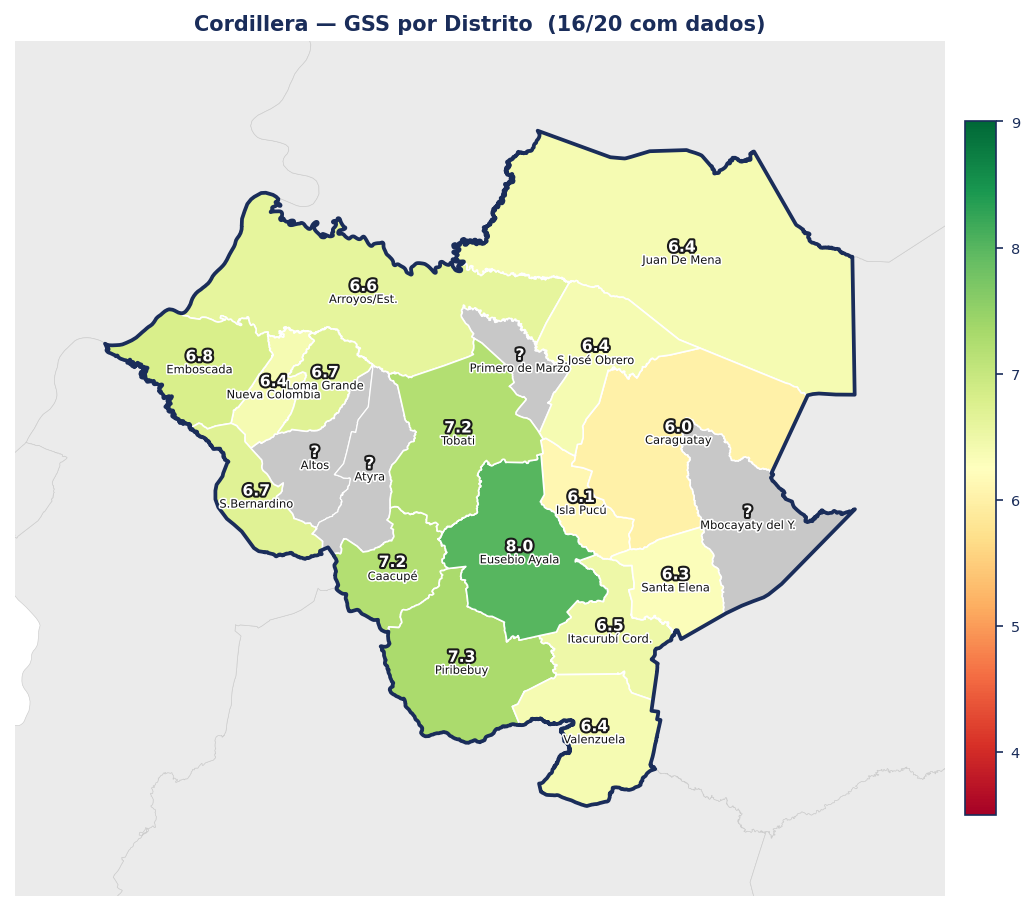
\includegraphics[width=\textwidth, height=0.55\textheight, keepaspectratio]{mapas/mapas_tematicos_dept_03_gss.png}
\caption{GSS (Global Safety Score) por distrito de Cordillera. Verde = alta viabilidade · Vermelho = baixa viabilidade.}
\label{fig:gss-03}
\end{figure}

\vspace{0.5em}

\begin{figure}[htbp]
\centering
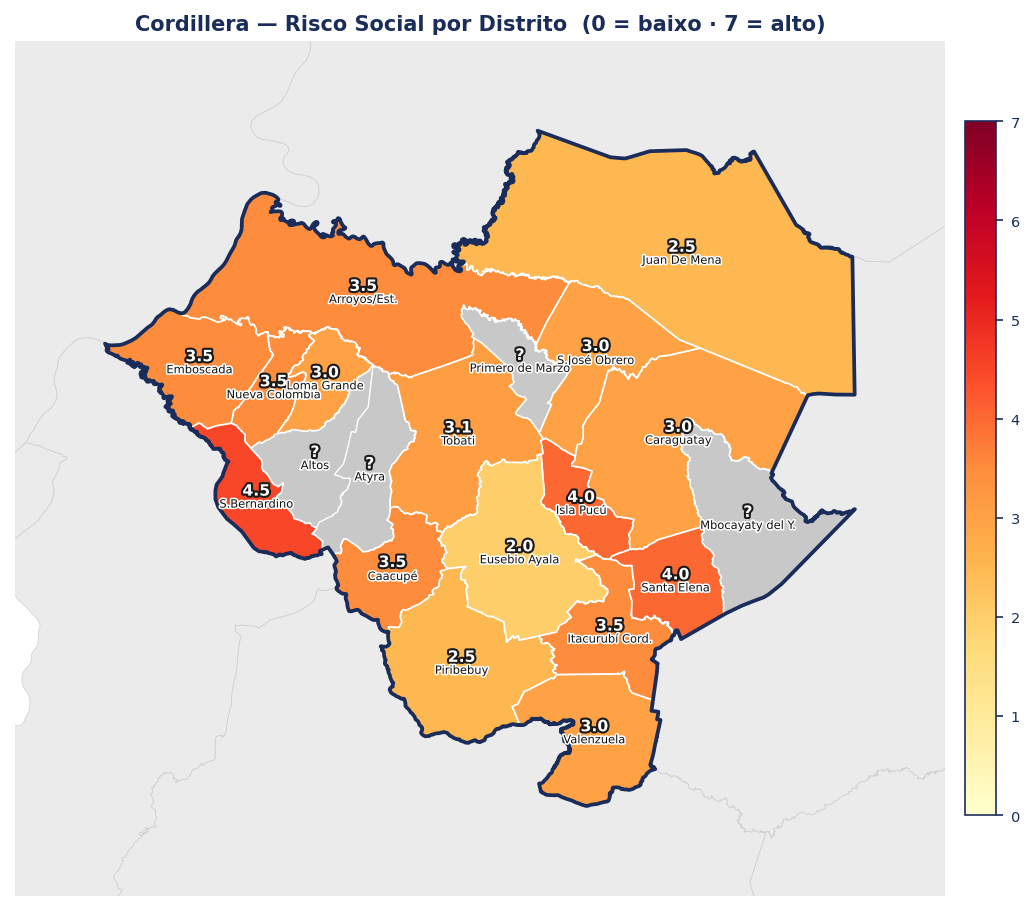
\includegraphics[width=\textwidth, height=0.55\textheight, keepaspectratio]{mapas/mapas_tematicos_dept_03_risco.png}
\caption{Risco social por distrito de Cordillera. Amarelo = baixo risco · Vermelho = alto risco.}
\label{fig:risco-03}
\end{figure}

\clearpage

\begin{figure}[htbp]
\centering
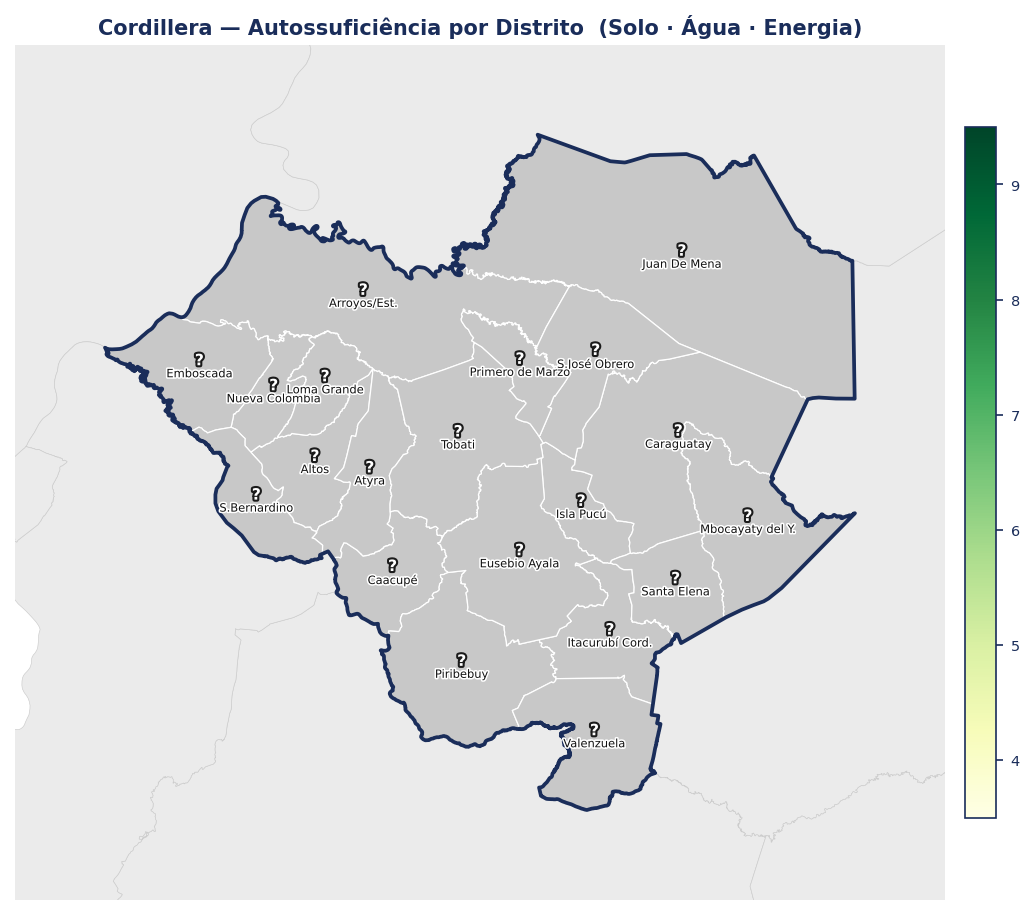
\includegraphics[width=\textwidth, height=0.55\textheight, keepaspectratio]{mapas/mapas_tematicos_dept_03_autosuf.png}
\caption{Autossuficiência por distrito de Cordillera: solo, recursos hídricos e potencial energético. Branco = baixo · Verde escuro = alto.}
\label{fig:autosuf-03}
\end{figure}

\clearpage

\section{Cordillera}

e uma malha territorial de transição entre a área metropolitana e o
interior produtivo.

\subsection{Ficha climática de Caacupe (capital
departamental)}

\textbf{Irradiância solar global --- (kWh/\allowbreak m²/\allowbreak dia):}


\begin{center}
\resizebox{\linewidth}{!}{%
{\renewcommand{\arraystretch}{1.2}%
\begin{tabular}{@{}c|c|c|c|c|c|c|c|c|c|c|c@{}}
\toprule
Jan & Fev & Mar & Abr & Mai & Jun & Jul & Ago & Set & Out & Nov & Dez \\
\midrule
6.76 & 6.20 & 5.42 & 4.44 & 3.36 & 2.83 & 3.21 & 3.93 & 4.61 & 5.49 &
6.42 & 6.78 \\
\bottomrule
\end{tabular}}%
}
\end{center}


Média anual: 4.95 kWh/\allowbreak m²/\allowbreak dia. Inclinação recomendada: 25° Norte (anual);
35° inverno; 15° verão.

\textbf{Precipitação --- (mm/\allowbreak mês):}


\begin{center}
\resizebox{\linewidth}{!}{%
{\renewcommand{\arraystretch}{1.2}%
\begin{tabular}{@{}c|c|c|c|c|c|c|c|c|c|c|c@{}}
\toprule
Jan & Fev & Mar & Abr & Mai & Jun & Jul & Ago & Set & Out & Nov & Dez \\
\midrule
127 & 140 & 133 & 148 & 152 & 78 & 66 & 41 & 77 & 171 & 193 & 175 \\
\bottomrule
\end{tabular}}%
}
\end{center}


Média anual: \textasciitilde1.500 mm/\allowbreak ano. Estação chuvosa Out-Mai; seca
Jun-Set.
\clearpage
\subsection*{Dados Departamentais}

\subsection*{Segurança Pública}

\begin{tabularx}{\linewidth}{lX}
\toprule
Indicador & Valor \\
\midrule
Taxa de homicídios (por 100k hab) & 3,5 (2022, fonte INE/Prosegur) \\
Crimes registrados (total/ano) & --- dados não desagregados publicamente \\
Número de comisarías & ~18 (estimativa departamental) \\
Índice segurança relativo & alto \\
\bottomrule
\end{tabularx}

Cordillera é um dos departamentos mais seguros do Paraguai. A taxa de homicídios de \textbf{3,5 por 100 mil habitantes} (2022) está significativamente abaixo da média nacional de 5,3 (2023) e muito abaixo dos departamentos fronteiriços problemáticos. O Ministerio Público registra que Cordillera responde por apenas \textbf{2\% das causas de homicídio doloso} do país --- proporção baixa considerando que é um departamento populoso próximo à capital.

O departamento não possui fronteira internacional e está geograficamente isolado de rotas principais de narcotráfico. Sua proximidade com Asunción (a capital está a menos de 80 km de Caacupé) facilita o acesso a serviços de segurança da capital. O turismo religioso em Caacupé (maior santuário mariano do Paraguai) gera movimentação econômica e maior presença policial em datas festivas.

A criminalidade predominante é patrimonial (furtos e roubos), especialmente em áreas com maior fluxo turístico. Violência com motivação de crimen organizado é rara no departamento.

\subsection*{IDH e Desenvolvimento Humano}

\begin{tabularx}{\linewidth}{lX}
\toprule
Indicador & Valor \\
\midrule
IDH & 0,718 \\
Classificação IDH & alto \\
Ranking nacional (1=melhor) & 6/18 \\
Esperança de vida & 73,5 anos \\
Anos de escolaridade média & 8,6 anos \\
RNB per capita (USD PPA) & 9.200 \\
\bottomrule
\end{tabularx}

> Nota: IDH estimado com base no relatório PNUD 2020 e dados subnacionais da Global Data Lab. Cordillera se beneficia da proximidade com Asunción e Central, apresentando IDH acima da média nacional. Estimativa com base nos dados publicados para a Região Central/Oriental paraguaia.

\begin{tabularx}{\linewidth}{lX}
\toprule
Indicador & Valor \\
\midrule
Taxa de pobreza total (\%) & 23,9\% \\
Taxa de pobreza extrema (\%) & 5,2\% \\
Índice de Gini & 0,440 \\
\bottomrule
\end{tabularx}

> Fonte: INE --- EPHC 2023 e Pobreza Multidimensional 2023 (IPM Cordillera: 20,22\%). Nota: houve aumento da pobreza em Cordillera entre 2022 e 2023 segundo relatório Última Hora.

\begin{tabularx}{\linewidth}{lX}
\toprule
Indicador & Valor \\
\midrule
Acesso a água potável (\%) & 82,4\% \\
Acesso a saneamento (\%) & 84,7\% \\
\bottomrule
\end{tabularx}

> Estimativa baseada no Censo 2022 e perfil semiurbano do departamento. Cordillera combina municípios turísticos (São Bernardino) com zonas rurais, resultando em cobertura heterogênea.

Cordillera é um departamento estrategicamente localizado entre Asunción e o interior do Paraguai, com IDH de 0,718 (alto). A proximidade com a capital (a apenas 50-70 km) permite acesso a serviços de saúde e educação de qualidade, enquanto o custo de vida é menor. Caacupé, capital departamental e sede do maior santuário mariano do Paraguai, oferece infraestrutura razoável. São Bernardino no lago Ypacaraí é área turística valorizada, com imóveis disputados e qualidade de vida elevada. Para brasileiros, Cordillera representa boa relação custo-benefício: mora-se com mais espaço e conforto do que em Asunción, com acesso às amenidades da capital. A pobreza de 23,9\% é moderada. Água (82,4\%) e saneamento (84,7\%) têm cobertura boa. Oportunidades em turismo, agropecuária e serviços de apoio à capital.

\subsection*{Sistema Prisional}

{\small
{\small
\begin{tabularx}{\linewidth}{lXXXX}
\toprule
Nome & Município & Capacidade & População & Superlotação \\
\midrule
Penitenciaría Regional de Caacupé & Caacupé & 180 & ~310 & ~172\% \\
\bottomrule
\end{tabularx}
}
}

\begin{tabularx}{\linewidth}{lX}
\toprule
Indicador & Valor \\
\midrule
Total de estabelecimentos & 1 \\
Capacidade total (vagas) & ~180 \\
População carcerária total & ~310 \\
Taxa de superlotação & ~172\% \\
\% presos provisórios & ~65\% \\
\bottomrule
\end{tabularx}

O departamento de Cordillera conta com uma única penitenciaría regional, localizada em Caacupé, capital departamental. Embora a superlotação seja significativa, o estabelecimento apresenta condições ligeiramente melhores do que os presídios de departamentos mais remotos, possivelmente devido à sua proximidade com Asunción (~54 km) e ao maior acesso a serviços.

Caacupé é o maior centro urbano do departamento e sede da Basílica de Nossa Senhora dos Milagres, o que torna a cidade um importante polo turístico-religioso. A atividade econômica diversificada do departamento --- agricultura, turismo, artesanato --- está associada a uma população carcerária predominantemente local, com menor influência de crime organizado transnacional em comparação com departamentos de fronteira.

Detentos de municípios menores como Tobatí, Eusebio Ayala, Piribebuy e San Bernardino são transferidos para Caacupé, dado que esses municípios não possuem estabelecimentos penais próprios.

\textbf{Para imigrantes:} Cordillera é um departamento relativamente seguro e com boa infraestrutura. A presença de presídio em Caacupé não impacta significativamente a segurança urbana. O departamento é considerado de baixo risco para instalação e residência.

\subsection*{Recursos Hídricos Subterrâneos}

\begin{tabularx}{\linewidth}{lXXX}
\toprule
Aquífero & Cobertura no Dept. & Profundidade Média & Vazão Típica \\
\midrule
Patiño (freático, porção norte) & ~30\% & 30--80 m & 5--15 m$^3$/h \\
Misiones / Guarani (confinado) & ~50\% & 120--400 m & 20--60 m$^3$/h \\
Cristalino (fraturado) & ~20\% (serras) & 30--80 m & 2--8 m$^3$/h \\
\bottomrule
\end{tabularx}

\begin{tabularx}{\linewidth}{lX}
\toprule
Parâmetro & Valor \\
\midrule
Profundidade média --- Patiño (m) & 30--80 \\
Profundidade média --- Guarani (m) & 120--400 \\
Profundidade máxima recomendada (m) & 400 \\
Vazão típica (m$^3$/h) & 5--40 \\
Custo estimado perfuração (USD) & 2.500 -- 10.000 \\
Qualidade da água --- Patiño & boa a moderada \\
Qualidade da água --- Guarani & boa a excelente \\
pH médio & 6,5--7,5 \\
Outorga necessária & sim \\
Órgão regulador & MADES --- DGPCRH \\
\bottomrule
\end{tabularx}

Cordillera faz limite com o Departamento Central e abriga parte do Aquífero Patiño em sua porção norte (continuidade em direção a Paraguarí). O Aquífero Guarani/Misiones está presente na metade sul e leste, com profundidades moderadas. A qualidade da água é boa em ambos os sistemas, com baixa mineralização. O departamento conta com cidades de porte médio como Caacupé (capital), onde o abastecimento público é operado por SENASA e cooperativas. Em zonas rurais, poços artesianos são amplamente utilizados para abastecimento doméstico e dessedentação animal. A Serra de Yhaguy e os afloramentos cristalinos oferecem captação em fraturas com boa qualidade.

Cordillera é um departamento atrativo para imigrantes pela proximidade com Asunción e clima agradável (altitude ~300 m). Poços no Aquífero Patiño (30--80 m) são a opção de menor custo para propriedades perto da capital --- estimativa de USD 2.500 a 6.000. Para chácaras no sul/leste do departamento, o Guarani (120--300 m) é acessível com custo de USD 5.000--10.000 e vazão abundante. Obrigatorio: licença do MADES. San Bernardino (lago Ypacaraí) tem rede pública de abastecimento razoável.

\subsection*{Aptidão do Solo}

\begin{tabularx}{\linewidth}{lXX}
\toprule
Tipo de Solo & \% do Território & Características \\
\midrule
Ultissolos (Argissolos) & 50\% & Solos podzólicos, textura areno-argilosa, profundidade variável, fertilidade baixa-média \\
Entissolos (Litossolos/Neossolos) & 25\% & Solos rasos sobre afloramentos rochosos da Cordilheira, limitados para agricultura \\
Inceptissolos & 15\% & Solos jovens em encostas, moderada fertilidade, suscetíveis à erosão \\
Aluviais (Entissolos flúvicos) & 10\% & Várzeas dos rios Salado e afluentes, potencial para hortas \\
\bottomrule
\end{tabularx}

\begin{tabularx}{\linewidth}{lXX}
\toprule
Classe & \% Território & Uso Recomendado \\
\midrule
Lavoura intensiva & 10\% & Horticultura, fruticultura em áreas de planície \\
Lavoura extensiva & 25\% & Mandioca, milho, amendoim \\
Pastagem natural & 30\% & Pecuária extensiva em áreas de encosta \\
Floresta / reserva & 20\% & Cobertura nativa residual, matas ciliares \\
Sem aptidão agrícola & 15\% & Áreas rochosas, urbanizadas (Caacupé, cidades satélites de Asunción) \\
\bottomrule
\end{tabularx}

\begin{tabularx}{\linewidth}{lX}
\toprule
Parâmetro & Valor \\
\midrule
pH médio & 5,0 -- 6,0 \\
Fertilidade natural & baixa \\
Teor de matéria orgânica & baixo \\
Necessidade de calcário & sim \\
\bottomrule
\end{tabularx}

Cordillera não é destino recomendado para imigrantes brasileiros com foco em agricultura em grande escala. O departamento apresenta solos entre os mais degradados do país, relevo acidentado e crescente pressão urbana. Eventuais oportunidades estão no turismo rural (Lago Ypacaraí, Caacupé), agroturismo e pequenas propriedades para produção de hortifruti. Para agricultura mecanizada, há opções muito melhores nos departamentos de Alto Paraná, Itapúa, Caaguazú ou San Pedro.

\subsection*{Terra Rural}

\begin{tabularx}{\linewidth}{lXXX}
\toprule
Tipo & Preço (USD/ha) & Faixa & Tendência \\
\midrule
Agrícola alta produtividade & 5.500 & 3.500 -- 8.000 & $\uparrow$ \\
Pastagem & 3.000 & 2.000 -- 4.500 & $\uparrow$ \\
Mata / reserva & 1.200 & 700 -- 2.000 & $\uparrow$ \\
\bottomrule
\end{tabularx}

\begin{tabularx}{\linewidth}{lX}
\toprule
Parâmetro & Valor \\
\midrule
Valorização anual média (\%) & 7--10\% \\
Lote mínimo rural (ha) & 10 \\
Imposto territorial rural (\%) & 1\% sobre valor fiscal \\
Liquidez do mercado & média--alta \\
\bottomrule
\end{tabularx}

\begin{tabularx}{\linewidth}{lXXX}
\toprule
Indicador & Cordillera (PY) & Santa Catarina - Serra (BR) & Rio Grande do Sul - Serra (BR) \\
\midrule
Terra agrícola (USD/ha) & 3.500--8.000 & 15.000--30.000 & 12.000--25.000 \\
Chácara lazer (USD/ha) & 5.000--12.000 & 20.000--50.000 & 15.000--35.000 \\
\bottomrule
\end{tabularx}

Cordillera combina proximidade com Asunción (30--80 km) com paisagens de serras e lagos, tornando-a atrativa para chácaras de lazer a preços muito inferiores às serras gaúchas ou catarinenses.

\subsection*{Mercado Imobiliário}

\textbf{Capital:} Caacupé

\begin{tabularx}{\linewidth}{lXX}
\toprule
Tipo & Preço (USD/m$^2$) & Aluguel (USD/mês) \\
\midrule
Apartamento 2 quartos & 700 -- 1.100 & 250 -- 500 \\
Casa 3 quartos & 600 -- 950 & 220 -- 450 \\
\bottomrule
\end{tabularx}

> Nota: San Bernardino, no mesmo departamento, tem preços significativamente mais altos --- apartamentos e casas entre USD 1.200--2.500/m$^2$ por ser destino turístico premium.

\begin{tabularx}{\linewidth}{lX}
\toprule
Parâmetro & Valor \\
\midrule
Valorização anual (\%) & 7--9\% \\
Disponibilidade de financiamento & boa (proximidade com Asunción facilita acesso a bancos nacionais) \\
Bairros mais valorizados & Centro de Caacupé, San Bernardino (orla do lago), Altos \\
\bottomrule
\end{tabularx}

\textbf{Vale a pena comprar ou alugar?}
Cordillera é um dos departamentos mais atrativos para imigrantes que trabalham remotamente ou visitam Asunción regularmente. A combinação de ar fresco de serra, paisagem agradável, segurança relativa e proximidade com a capital (30--80 km) torna a compra de casa ou chácara especialmente vantajosa.

\textbf{Áreas recomendadas:}
Caacupé (turismo religioso, serviços consolidados) e San Bernardino (orla do Lago Ypacaraí, segunda residência) são as melhores opções do departamento. San Bernardino é particularmente atrativa para quem busca qualidade de vida com fácil acesso a Asunción (50 km).

\textbf{Armadilhas comuns:}
Imóveis próximos ao Lago Ypacaraí estão sujeitos a restrições ambientais da SEAM (hoje MADES) que podem impedir construções ou reformas. Solicite sempre o certificado de conformidade ambiental antes de fechar qualquer negócio na faixa ribeirinha.

\subsection*{Cobertura Celular}

{\small
{\small
\begin{tabularx}{\linewidth}{lXXXXX}
\toprule
Operadora & 2G & 3G & 4G & 5G & Cobertura Pop. \\
\midrule
Tigo & 95\% & 90\% & 85\% & --- & 92\% \\
Personal/Claro & 90\% & 85\% & 78\% & --- & 88\% \\
VOX & 65\% & 50\% & 35\% & --- & 60\% \\
\bottomrule
\end{tabularx}
}
}

> \textbf{Nota:} Cordillera é um dos departamentos mais bem servidos fora da região metropolitana. A proximidade com Asunción (capital Caacupé está a 54 km) garante boa infraestrutura. 4G disponível em praticamente todas as cidades do departamento. Apenas áreas serranas isoladas têm cobertura reduzida.

\begin{tabularx}{\linewidth}{lX}
\toprule
Parâmetro & Valor \\
\midrule
Melhor operadora rural & Tigo \\
Velocidade 4G média (Mbps) & 25--45 \\
Áreas sem cobertura & Serras isoladas, algumas propriedades rurais no norte do departamento \\
Sinal em propriedade rural & bom a moderado \\
\bottomrule
\end{tabularx}

\begin{tabularx}{\linewidth}{lXXX}
\toprule
Plano & Operadora & USD/mês & Dados \\
\midrule
Pré-pago básico (7 dias) & Tigo & ~2,50 & 3 GB \\
Pré-pago intermediário (30 dias) & Personal & ~5,00 & 8 GB \\
Pós-pago entrada & Tigo & ~12,00 & 15 GB + chamadas \\
Pós-pago intermediário & Personal/Claro & ~18,00 & 30 GB + chamadas \\
\bottomrule
\end{tabularx}

\subsection*{Internet}

\begin{tabularx}{\linewidth}{lX}
\toprule
Indicador & Valor \\
\midrule
\% população com internet & ~72\% \\
\% com banda larga fixa & ~35\% dos domicílios \\
Velocidade média download (Mbps) & 40--80 (urbano) / 8--25 (rural) \\
Velocidade média upload (Mbps) & 12--30 (urbano) \\
\bottomrule
\end{tabularx}

> Cordillera está entre os departamentos com melhor conectividade fora da região metropolitana, beneficiado pela proximidade com Asunción e pela Ruta 2 que conecta o departamento.

\begin{tabularx}{\linewidth}{lXX}
\toprule
Tecnologia & Disponibilidade & Velocidade Típica \\
\midrule
Fibra ótica (FTTH) & Caacupé, San Bernardino, Coronel Martínez, Eusebio Ayala & 50--500 Mbps \\
Cabo HFC & Caacupé e municípios principais & 30--200 Mbps \\
Rádio/Wireless & Amplo em todo o departamento & 5--50 Mbps \\
ADSL (Copaco) & Interior com rede legada & 2--10 Mbps \\
Satélite (Starlink) & Todo o departamento & 50--200 Mbps \\
\bottomrule
\end{tabularx}

\begin{tabularx}{\linewidth}{lXXX}
\toprule
Provedor & Tecnologia & Área de cobertura & Preço ref. (USD/mês) \\
\midrule
Tigo & Fibra/HFC/Rádio & Toda a região urbana & 18--55 \\
Claro/Personal & Fibra/Rádio & Caacupé e municípios maiores & 15--50 \\
Copaco & ADSL/Fibra & Interior + municípios menores & 10--30 \\
Starlink & Satélite LEO & Todo o departamento & ~44 + equip. ~370 \\
\bottomrule
\end{tabularx}

A cobertura de internet no interior de Cordillera é \textbf{moderada a boa}, especialmente ao longo da Ruta 2 (Asunción--Coronel Oviedo). Características:

Cordillera é um dos departamentos mais acessíveis para imigrantes em termos de conectividade rural, combinando boa cobertura celular 4G com opções de internet fixa razoáveis.

\clearpage
\newpage
\secaoDiagnostico{Altos}{\mapaDistrito{0302}}{Altos é o distrito mais elevado de Cordillera e um dos destinos
turísticos mais apreciados do Paraguai graças à sua Cordillera de los
Altos, que alcança 300--450\,m acima do nível do mar. A altitude confere
ao município um microclima notavelmente mais fresco que o da capital,
tornando-o atrativo para famílias e artesãos tradicionais. A produção de
\emph{ñandutí} (renda de bilro) e cerâmica artesanal constitui identidade
cultural forte. Para fins de relocação estratégica, Altos oferece
vantagem tática natural pela elevação, bom potencial hídrico em aquífero
cristalino fraturado, irradiação solar excelente e criminalidade muito
baixa, tudo a apenas 45\,km de Assunção pela PY02.

\subsubsection{Recomendação Técnica}

Indicado para residência permanente de perfil semirrural-turístico com
boa qualidade de vida. A combinação de altitude protetora contra
inundações, clima mais ameno, cobertura 4G Tigo sólida e proximidade
com a capital confere ao distrito GSS 7.0 — viável para relocação
familiar com infraestrutura básica consolidada. Priorizar terrenos em
cotas acima de 300\,m, instalar sistema solar fotovoltaico para autonomia
energética e garantir poço em aquífero cristalino (40--120\,m). O
mercado imobiliário serrano tende à valorização contínua pelo turismo.

}
\begin{table}[ht!]
\small \begin{tabular}{p{3.0cm}p{0.8cm}p{6.0cm}} \toprule
\textbf{Critério} & \textbf{Nota} & \textbf{Justificativa} \\ \midrule
A - Ameaças Estratégicas & 6.5 & Relativa proximidade com Assunção (45\,km); altitude oferece vantagem tática natural; sem alvos militares de relevo no perímetro imediato \\
B - Risco Social & 7.5 & Baixa densidade populacional; comunidade local estável com forte coesão religiosa e artesanal; turismo controlado; longe das favelas metropolitanas \\
C - Riscos Naturais & 7.5 & Altitude (300--450\,m) protege integralmente de inundações; clima mais fresco reduz riscos de calor extremo; sem atividade sísmica relevante; boa precipitação anual \\
D - Autossuficiência & 7.0 & Solo moderado (pH 5.0--6.0) apto para hortas e fruticultura; aquífero cristalino com boa qualidade; irradiação solar excelente (4.94 kWh/m²/dia); hortas e pomares viáveis \\
E - Institucional & 7.0 & Departamento Cordillera com IDH 0,728 sólido; serviços básicos de saúde e educação presentes; proximidade com Assunção para especialidades médicas \\
\midrule
 \textbf{GSS FINAL} & \textbf{7.0} & \textbf{Viável (Refúgio serrano de qualidade com boa relação custo-benefício; destaque para altitude protetora, clima ameno e baixa criminalidade).} \\ \bottomrule
 \end{tabular}
\end{table}
\subsubsection{Vulnerabilidades e Mitigação}\label{vuln-altos-0302}

\begin{itemize}
\tightlist
\item
  \textbf{Proximidade com a Capital:} A 45\,km de Assunção, o distrito
  pode sofrer pressão migratória em crises metropolitanas severas
  (Mitigação: escolher propriedades em áreas serranas interiores, longe
  das vias principais de fuga urbana; manter discrição social).
\item
  \textbf{Aquífero Cristalino Fraturado:} Poços em rocha fraturada
  exigem perfuração adequada e podem ter vazão variável conforme a
  estação (Mitigação: dimensionar cisterna de reserva para 30 dias;
  contratar hidrogeólogo local para posicionamento do poço).
\item
  \textbf{Solo Ácido com Fertilidade Média:} pH 5.0--6.0 e presença de
  laterita limitam culturas sensíveis à acidez (Mitigação: calagem
  periódica; focar em culturas adaptadas como mandioca, banana, maracujá
  e horticultura com canteiros elevados).
\item
  \textbf{Risco de Incêndio em Inverno Seco:} Vegetação serrana resseca
  em jun-ago quando a precipitação cai a 40--70\,mm/mês (Mitigação:
  manter aceiros limpos; instalar reservatório de água dedicado ao
  combate a incêndio).
\item
  \textbf{Valorização Imobiliária pelo Turismo:} A popularidade turística
  pode encarecer terrenos em zonas de vista privilegiada (Mitigação:
  buscar propriedades em micro-regiões menos turísticas do município,
  afastadas dos mirantes mais conhecidos).
\end{itemize}

\subsubsection{Dossiê de Campo}\label{dossie-altos-0302}
\begin{description}[style=nextline,leftmargin=0.5cm,font=\bfseries]
\item[Coordenadas]  25°16'S 57°29'W.
\item[Topografia]  Relevo serrano 300--450\,m de altitude; ponto mais elevado da Cordillera de los Altos; área \textasciitilde440\,km²; topografia ondulada com morros e vales; estável geologicamente.
\item[Alvos Estratégicos]  Nenhum alvo militar de relevo; altitude serrana confere vantagem tática natural de observação e defesa passiva; principais estruturas são de caráter turístico e artesanal.
\item[Fallout]  Ventos predominantes do NE; posição elevada favorece dispersão de contaminantes provenientes da planície metropolitana; distância e altitude mitigam riscos de fallout oriundo de Assunção.
\item[População]  \textasciitilde35.500 habitantes (Censo 2022). Comunidade mista de artesãos tradicionais, agricultores familiares e moradores de zona turística; forte presença religiosa (Mission Alliance, Mennonite).
\item[Densidade]  \textasciitilde80 hab/\allowbreak km² — moderada; permite privacidade em propriedades rurais sem isolamento excessivo.
\item[Vias de Acesso]  PY02 a 45\,km de Assunção (Ruta 2 Mariscal Estigarribia); estradas serranas pavimentadas e vicinais de cascalho; acesso ao Lago Ypacaraí a \textasciitilde15\,km via Areguá.
\item[Serviços]  Hospital distrital; posto de saúde USF; escolas públicas; ANDE (energia elétrica); comércio local básico; farmácias; correos.
\item[Custo de Vida]  Baixo a médio; turismo aquece preços de imóveis nas zonas serranas de vista, mas áreas rurais interiores permanecem acessíveis.
\item[Preço da Terra]  US\$~3.000--8.000/\allowbreak ha (rural serrana); USD~30--80/\allowbreak m² (urbano e zona turística).
\item[Hidrologia]  Aquífero Cristalino (fraturado) a 40--120\,m de profundidade; qualidade da água boa; acesso parcial ao Sistema Aquífero Guarani em camadas mais profundas; risco de inundação praticamente nulo pela altitude.
\item[Clima]  Subtropical com influência altitudinal; temperaturas médias 2--4°C inferiores às de Assunção; verões amenos, invernos frescos; precipitação anual de \textasciitilde1.418\,mm com estação seca branda (jun-ago).
\item[Energia]  ANDE (rede nacional Itaipu); fornecimento estável; potencial solar fotovoltaico excelente (média 4,94 kWh/m²/dia); altitude favorece rendimento dos painéis.
\item[Água]  Aquífero cristalino fraturado a 40--120\,m; qualidade boa; recomenda-se análise microbiológica e física-química antes do consumo; nascentes naturais pontuais nas encostas serranas.
\item[Qualidade do Solo]  Alfissolos e Ultissolos com laterita; pH 5.0--6.0; fertilidade média; aptidão para hortas com calagem, fruticultura (banana, maracujá, citros), pastagem e pecuária de pequeno porte.
\item[Recursos Locais]  Artesanato \emph{ñandutí} (renda de bilro, IG reconhecida); cerâmica tradicional; turismo serrano e ecoturismo; fruticultura tropical de altitude; mel; café em pequena escala.
\item[Segurança]  Criminalidade muito baixa; área serrana e turística com forte coesão social; presença policial adequada ao porte do município; sem registros de crime organizado ou narcotráfico local.
\item[Leis Local]  Município consolidado. \\ \textbf{Livre de Restrição} de Fronteira.
\end{description}
\textbf{Fonte climática:} NASA POWER Climatology API (período 2001-2020)

\textbf{Fonte luminosa:} estimativa world atlas

\paragraph{Irradiação Solar (kWh/\allowbreak m²/\allowbreak dia)}


\begin{center}
\resizebox{\linewidth}{!}{%
{\renewcommand{\arraystretch}{1.2}%
\begin{tabular}{@{}c|c|c|c|c|c|c|c|c|c|c|c|c@{}}
\toprule
Jan & Fev & Mar & Abr & Mai & Jun & Jul & Ago & Set & Out & Nov & Dez & Média \\
\midrule
6.75 & 6.15 & 5.40 & 4.45 & 3.37 & 2.82 & 3.20 & 3.92 & 4.60 & 5.47 &
6.40 & 6.77 & \textbf{4.94} \\
\bottomrule
\end{tabular}}%
}
\end{center}


\textbf{Inclinação solar recomendada:} 25° N (anual) · 35° N (inverno
jun-ago) · 15° N (verão nov-jan)

\paragraph{Precipitação (mm/\allowbreak mês)}


\begin{center}
\resizebox{\linewidth}{!}{%
{\renewcommand{\arraystretch}{1.2}%
\begin{tabular}{@{}c|c|c|c|c|c|c|c|c|c|c|c|c@{}}
\toprule
Jan & Fev & Mar & Abr & Mai & Jun & Jul & Ago & Set & Out & Nov & Dez & Total/\allowbreak ano \\
\midrule
120 & 130 & 125 & 145 & 140 & 70 & 58 & 40 & 70 & 160 & 185 & 175 &
\textbf{1.418 mm} \\
\bottomrule
\end{tabular}}%
}
\end{center}


\paragraph{Poluição Luminosa}

\begin{longtable}[]{@{}ll@{}}
\toprule\noalign{}
Parâmetro & Valor \\
\midrule\noalign{}
\endhead
\bottomrule\noalign{}
\endlastfoot
Escala Bortle & 3 --- Céu rural \\
Radiância artificial & 1.2 nW/\allowbreak cm²/\allowbreak sr \\
\end{longtable}
\paragraph{Solo (SoilGrids 2.0, média ponderada 0--30 cm)}

\begin{longtable}[]{@{}ll@{}}
\toprule\noalign{}
Parâmetro & Valor \\
\midrule\noalign{}
\endhead
\bottomrule\noalign{}
\endlastfoot
pH (H$_2$O) & 5.0--6.0 \\
Carbono orgânico (SOC) & 15--28 g/\allowbreak kg \\
Argila & 35--50 \% \\
Areia & 25--40 \% \\
Classe taxonômica & Ultissolo/\allowbreak Alfissolo com laterita \\
\textbf{Aptidão agrícola} & \textbf{Média} (calagem recomendada) \\
\end{longtable}

\subsubsection{Indicadores Sociais}

\textbf{Fontes:} PNUD 2020, INE\footnote{\fineINE} Censo 2022, INE\footnote{\fineINE} EPHC 2023, Ministerio
Público 2024\\
\textbf{Nota:} Valores marcados como \emph{(dept.)} referem-se ao
departamento de Cordillera; valores \emph{(dist.)} são específicos deste
distrito. Dados marcados \emph{(est.)} são estimativas.

\begin{longtable}[]{@{}
  >{\raggedright\arraybackslash}p{(\linewidth - 4\tabcolsep) * \real{0.4231}}
  >{\raggedright\arraybackslash}p{(\linewidth - 4\tabcolsep) * \real{0.2692}}
  >{\raggedright\arraybackslash}p{(\linewidth - 4\tabcolsep) * \real{0.3077}}@{}}
\toprule\noalign{}
\begin{minipage}[b]{\linewidth}\raggedright
Indicador
\end{minipage} & \begin{minipage}[b]{\linewidth}\raggedright
Valor
\end{minipage} & \begin{minipage}[b]{\linewidth}\raggedright
Âmbito
\end{minipage} \\
\midrule\noalign{}
\endhead
\bottomrule\noalign{}
\endlastfoot
IDH (2020) & 0,728 & dept.~(est.) \\
Ranking IDH nacional & 6/\allowbreak 18 & dept. \\
Esperança de vida & 73,5 anos & dept. \\
Escolaridade média & 8.4 anos & dist.~(est.) \\
RNB per capita (USD PPA) & 9.200 & dept. \\
Pobreza monetária (\%) & 23,9\% & dept. \\
Pobreza extrema (\%) & 5,2\% & dept. \\
Índice de Gini & 0,440 & dept. \\
Acesso a água potável (\%) & 82,4\% & dept. \\
Acesso a saneamento (\%) & 84,7\% & dept. \\
Taxa de homicídios (est., /\allowbreak 100k hab) & 3,5 (2022, fonte INE\footnote{\fineINE}/\allowbreak Prosegur) &
dept. \\
Índice de segurança & muito alto & dist. \\
População (Censo 2022) & \textasciitilde35.500 hab. & dist. \\
Idade mediana & 28.5 anos & dist.~(est.) \\
Taxa de fecundidade & N/\allowbreak D & dist. \\
\end{longtable}
\subsubsection{Combustível}

\textbf{Referência:} PETROPAR /\allowbreak  postos locais (2024) \textbf{Tipo de
localidade:} Interior

\begin{longtable}[]{@{}lll@{}}
\toprule\noalign{}
Combustível & USD/\allowbreak litro & Gs/\allowbreak litro (aprox.) \\
\midrule\noalign{}
\endhead
\bottomrule\noalign{}
\endlastfoot
Gasolina 93 oct & 0.96 & 7,104 \\
Gasolina 97 oct (premium) & 1.06 & 7,844 \\
Diesel & 0.89 & 6,586 \\
\end{longtable}

\begin{quote}
Preços podem variar ±5\% conforme posto e sazonalidade. Chaco e interior
remoto apresentam maior variação.
\end{quote}

\subsubsection{Cobertura Celular}

\textbf{Fonte:} CONATEL PY /\allowbreak  operadoras (2024)

\begin{longtable}[]{@{}ll@{}}
\toprule\noalign{}
Parâmetro & Valor \\
\midrule\noalign{}
\endhead
\bottomrule\noalign{}
\endlastfoot
Cobertura 4G população (dept.) & 90\% \\
Cobertura 4G área rural & 78\% \\
Melhor operadora & Tigo \\
Qualidade rural & boa \\
\end{longtable}

\begin{quote}
Cobertura Tigo 4G sólida na área urbana e nas principais estradas
serranas; zonas de encosta mais fechadas podem exigir Starlink como
backup.
\end{quote}

\subsubsection{Internet}

\textbf{Fonte:} CONATEL /\allowbreak  Speedtest Ookla (2024)

\begin{longtable}[]{@{}ll@{}}
\toprule\noalign{}
Parâmetro & Valor \\
\midrule\noalign{}
\endhead
\bottomrule\noalign{}
\endlastfoot
Velocidade média download & 45 Mbps \\
Domicílios com internet (dept.) & 65\% \\
Tecnologia predominante & rádio/\allowbreak fibra \\
Opção rural & Starlink disponível (\textasciitilde USD 44/\allowbreak mês) \\
\end{longtable}

\subsubsection{Mercado Imobiliário e Terra Rural}

\textbf{Fonte:} INDERT /\allowbreak  Clasificados.com.py (2024)

\begin{longtable}[]{@{}ll@{}}
\toprule\noalign{}
Tipo & Referência \\
\midrule\noalign{}
\endhead
\bottomrule\noalign{}
\endlastfoot
Terra rural serrana (USD/\allowbreak ha) & 3.000--8.000 \\
Imóvel urbano (USD/\allowbreak m²) & 30--80 \\
Aluguel 2 quartos (USD/\allowbreak mês) & 200--350 \\
\end{longtable}

\begin{quote}
Preços da zona serrana com vista tendem à valorização pelo turismo; áreas
rurais interiores e de menor visibilidade permanecem entre os mais
acessíveis do departamento.
\end{quote}

\subsubsection{Saúde}

\textbf{Fonte:} MSPBS /\allowbreak  IPS Paraguay (2024-2026), consolidação
departamental e proxy local

\begin{longtable}[]{@{}ll@{}}
\toprule\noalign{}
Serviço & Disponibilidade \\
\midrule\noalign{}
\endhead
\bottomrule\noalign{}
\endlastfoot
USF /\allowbreak  Posto de Saúde & sim \\
Hospital Distrital & sim \\
IPS (seguro social) & não \\
Farmácia & sim \\
Distância ao hospital de referência & \textasciitilde45 km (Assunção) / \textasciitilde25 km (Caacupé) \\
\end{longtable}

\textbf{Principais estabelecimentos:} Hospital Distrital de Altos; USF local;
referência hospitalar em Caacupé ou Assunção para especialidades.

\textbf{Observação para imigrantes:} Atendimento primário e urgências
disponíveis localmente; especialidades e cirurgias de maior complexidade
requerem deslocamento até Caacupé (\textasciitilde25\,km) ou Assunção
(\textasciitilde45\,km). Cobertura privada recomendada para maior
abrangência.
\newpage
\secaoDiagnostico{Arroyos y Esteros}{\mapaDistrito{0303}}{Arroyos y Esteros é um polo de produção orgânica com excelente
conectividade logística, mas que exige atenção rigorosa à sua
hidrografia. É uma opção sólida para quem busca autossuficiência
agrícola, desde que o terreno seja escolhido fora das áreas de inundação
dos esteros.

\subsubsection{Analise de Sensibilidade}

\begin{itemize}
\tightlist
\item
  \textbf{Otimista (Melhoria infra):} GSS 6.9
\item
  \textbf{Conservador (Crise hídrica/\allowbreak cheias):} GSS 6.2
\end{itemize}

}
\begin{table}[ht!]
\small \begin{tabular}{p{3.0cm}p{0.8cm}p{6.0cm}} \toprule
\textbf{Critério} & \textbf{Nota} & \textbf{Justificativa} \\ \midrule
A - Ameaças Estratégicas & 7.0 & - \\
B - Risco Social & 6.5 & - \\
C - Riscos Naturais & 5.0 & - \\
D - Autossuficiência & 7.5 & - \\
E - Institucional & 6.5 & - \\
\midrule
 \textbf{GSS FINAL} & \textbf{6.6} & \textbf{Moderadamente Seguro (Exige preparação intensiva contra inundações).} \\ \bottomrule
 \end{tabular}
\end{table}
\subsubsection{Vulnerabilidades e
Mitigação}\label{vuln-arroyos-y-esteros-0303}

\begin{itemize}
\item
  \textbf{Risco de Inundação:} Priorizar construção em cotas elevadas
  (\textgreater80m). Sistemas de drenagem e estoque de emergência para
  períodos de isolamento rural.
\item
  \textbf{Eixo Logístico:} Em caso de crise nacional, a PY03 será alvo
  de controle severo. Manter rotas vicinais mapeadas para fuga ou
  abastecimento discreto.
\item
  \textbf{Contaminação Hídrica:} Filtragem avançada necessária para água
  superficial; preferência por poços profundos protegidos.
\item
  Censo 2022: 20.347 habitantes.
\item
  Preço terra: USD 5.200 - 8.000/\allowbreak ha.
\item
  Solo: Ultisoles/\allowbreak Areias Quartzosas.
\item
  Homicídios: 3-5/\allowbreak 100k hab (Cordillera).
\item
  Hospital: IPS Puesto Sanitario + Centros MSPyBS.
\end{itemize}
\subsubsection{Dossiê de Campo}\label{dossie-arroyos-y-esteros-0303}
\begin{description}[style=nextline,leftmargin=0.5cm,font=\bfseries]
\item[Coordenadas]  25°04'S 57°06'W.
\item[Topografia]  Relevo de baixada, com presença de numerosos arroios e extensas áreas de pântanos (esteros). Altitude \textasciitilde 70m.
\item[Alvos Estratégicos]  Indústria de açúcar orgânico (líder mundial), Porto de carga no Rio Manduvirá, Eixo logístico da Ruta PY03.
\item[Fallout]  Ventos predominantes do Norte/\allowbreak Nordeste.
\item[Fontes] Censo CNPV2022 (DGEEC); SEAM; Municipalidad de Arroyos y Esteros.
\item[População]  20.347 (Censo 2022 Final).
\item[Densidade]  \textasciitilde 37,89 hab/\allowbreak km².
\item[Vias de Acesso]  Localização privilegiada sobre a Ruta PY03. Importante conexão entre Central e o Norte. Recentemente inaugurado trecho asfáltico Arroyos y Esteros - Cañada Costa Pucú.
\item[Serviços]  Puesto Sanitario do IPS modernizado (urgências, pediatria, ginecologia). Centros de saúde do MSPyBS.
\item[Fontes] Censo CNPV2022 (DGEEC); SEAM; Municipalidad de Arroyos y Esteros.
\item[Hidrologia]  Risco Crítico de inundação. A combinação do Rio Manduvirá com os esteros locais torna o distrito vulnerável a cheias prolongadas.
\item[Sismicidade]  Risco muito baixo. Zona intraplaca estável.
\item[Clima]  Subtropical Úmido com alta umidade relativa devido à hidrografia.
\item[Fontes] Censo CNPV2022 (DGEEC); SEAM; Municipalidad de Arroyos y Esteros.
\item[Energia]  Rede nacional (Itaipu).
\item[Água]  Abundância de recursos hídricos superficiais (Manduvirá), porém sujeitos a contaminação. Poços artesianos são recomendados.
\item[Solo]  Predomínio de solos Podzólicos (Ultisoles) e Areias Quartzosas. Alta aptidão para cana-de-açúcar orgânica e pecuária.
\item[Preço da Terra]  Gs. 40-60 milhões/\allowbreak ha (USD 5.200 - 8.000). Propriedades premium até USD 11.000/\allowbreak ha.
\item[Fontes] Censo CNPV2022 (DGEEC); SEAM; Municipalidad de Arroyos y Esteros.
\item[Segurança]  Cordillera é um dos departamentos mais seguros. Taxa de homicídios entre 3-5 por 100k hab (abaixo da média nacional de 6.5).
\item[Leis Local]  Município histórico com tradição agrícola.
\item[Fontes] Censo CNPV2022 (DGEEC); SEAM; Municipalidad de Arroyos y Esteros.
\end{description}
\textbf{Fonte climática:} NASA POWER Climatology API (período 2001-2020)

\textbf{Fonte luminosa:} estimativa world atlas

\paragraph{Irradiação Solar
(kWh/\allowbreak m²/\allowbreak dia)}


\begin{center}
\resizebox{\linewidth}{!}{%
{\renewcommand{\arraystretch}{1.2}%
\begin{tabular}{@{}c|c|c|c|c|c|c|c|c|c|c|c|c@{}}
\toprule
Jan & Fev & Mar & Abr & Mai & Jun & Jul & Ago & Set & Out & Nov & Dez & Média \\
\midrule
6.76 & 6.20 & 5.42 & 4.44 & 3.36 & 2.83 & 3.21 & 3.93 & 4.61 & 5.49 &
6.42 & 6.78 & \textbf{4.95} \\
\bottomrule
\end{tabular}}%
}
\end{center}


\textbf{Inclinação solar recomendada:} 25° N (anual) · 35° N (inverno
jun-ago) · 15° N (verão nov-jan)

\paragraph{Precipitação (mm/\allowbreak mês)}


\begin{center}
\resizebox{\linewidth}{!}{%
{\renewcommand{\arraystretch}{1.2}%
\begin{tabular}{@{}c|c|c|c|c|c|c|c|c|c|c|c|c@{}}
\toprule
Jan & Fev & Mar & Abr & Mai & Jun & Jul & Ago & Set & Out & Nov & Dez & Total/\allowbreak ano \\
\midrule
124 & 146 & 126 & 144 & 156 & 79 & 64 & 38 & 79 & 172 & 195 & 174 &
\textbf{1501 mm} \\
\bottomrule
\end{tabular}}%
}
\end{center}


\paragraph{Poluição Luminosa}

\begin{longtable}[]{@{}ll@{}}
\toprule\noalign{}
Parâmetro & Valor \\
\midrule\noalign{}
\endhead
\bottomrule\noalign{}
\endlastfoot
Escala Bortle & 4 --- Céu rural-suburbano \\
Radiância artificial & 3.0 nW/\allowbreak cm²/\allowbreak sr \\
\end{longtable}
\paragraph{Solo (SoilGrids 2.0, média ponderada 0--30
cm)}

\begin{longtable}[]{@{}ll@{}}
\toprule\noalign{}
Parâmetro & Valor \\
\midrule\noalign{}
\endhead
\bottomrule\noalign{}
\endlastfoot
pH (H$_2$O) & 5.6 \\
Carbono orgânico (SOC) & 17.75 g/\allowbreak kg \\
Argila & 25.58 \% \\
Areia & 53.18 \% \\
Silte (calc.) & 21.2 \% \\
Densidade aparente & 1.32 g/\allowbreak cm³ \\
\textbf{Aptidão agrícola} & \textbf{Alta} \\
\end{longtable}

\begin{itemize}
\tightlist
\item
  \textbf{Preço da Terra:} Gs. 40-60 milhões/\allowbreak ha (USD 5.200 - 8.000).
  Propriedades premium até USD 11.000/\allowbreak ha.
\item
  \textbf{Fontes:}
\end{itemize}
\subsubsection{Indicadores Sociais}

\textbf{Fontes:} PNUD 2020, INE\footnote{\fineINE} Censo 2022, INE\footnote{\fineINE} EPHC 2023, Ministerio
Público 2024\\
\textbf{Nota:} Valores marcados como \emph{(dept.)} referem-se ao
departamento de Cordillera; valores \emph{(dist.)} são específicos deste
distrito. Dados marcados \emph{(est.)} são estimativas.

\begin{longtable}[]{@{}
  >{\raggedright\arraybackslash}p{(\linewidth - 4\tabcolsep) * \real{0.4231}}
  >{\raggedright\arraybackslash}p{(\linewidth - 4\tabcolsep) * \real{0.2692}}
  >{\raggedright\arraybackslash}p{(\linewidth - 4\tabcolsep) * \real{0.3077}}@{}}
\toprule\noalign{}
\begin{minipage}[b]{\linewidth}\raggedright
Indicador
\end{minipage} & \begin{minipage}[b]{\linewidth}\raggedright
Valor
\end{minipage} & \begin{minipage}[b]{\linewidth}\raggedright
Âmbito
\end{minipage} \\
\midrule\noalign{}
\endhead
\bottomrule\noalign{}
\endlastfoot
IDH (2020) & 0,718 & dept. \\
Ranking IDH nacional & 6/\allowbreak 18 & dept. \\
Esperança de vida & 73,5 anos & dept. \\
Escolaridade média & 8.2 anos & dist. \\
RNB per capita (USD PPA) & 9.200 & dept. \\
Pobreza monetária (\%) & 23,9\% & dept. \\
Pobreza extrema (\%) & 5,2\% & dept. \\
Índice de Gini & 0,440 & dept. \\
Acesso a água potável (\%) & 82,4\% & dept. \\
Acesso a saneamento (\%) & 84,7\% & dept. \\
Taxa de homicídios (est., /\allowbreak 100k hab) & 3,5 (2022, fonte INE\footnote{\fineINE}/\allowbreak Prosegur) &
dept. \\
Índice de segurança & alto & dept. \\
População (Censo 2022) & 20.347 hab. & dist. \\
Idade mediana & 30.0 anos & dist. \\
Taxa de fecundidade & N/\allowbreak D & dist. \\
\end{longtable}
\subsubsection{Combustível}

\textbf{Referência:} PETROPAR /\allowbreak  postos locais (2024) \textbf{Tipo de
localidade:} Interior

\begin{longtable}[]{@{}lll@{}}
\toprule\noalign{}
Combustível & USD/\allowbreak litro & Gs/\allowbreak litro (aprox.) \\
\midrule\noalign{}
\endhead
\bottomrule\noalign{}
\endlastfoot
Gasolina 93 oct & 0.96 & 7,104 \\
Gasolina 97 oct (premium) & 1.06 & 7,844 \\
Diesel & 0.89 & 6,586 \\
\end{longtable}

\begin{quote}
Preços podem variar ±5\% conforme posto e sazonalidade. Chaco e interior
remoto apresentam maior variação.
\end{quote}

\subsubsection{Cobertura Celular}

\textbf{Fonte:} CONATEL PY /\allowbreak  operadoras (2024)

\begin{longtable}[]{@{}ll@{}}
\toprule\noalign{}
Parâmetro & Valor \\
\midrule\noalign{}
\endhead
\bottomrule\noalign{}
\endlastfoot
Cobertura 4G população (dept.) & 90\% \\
Cobertura 4G área rural & 78\% \\
Melhor operadora & Tigo \\
Qualidade rural & boa \\
\end{longtable}

\begin{quote}
Para áreas rurais fora do núcleo urbano, recomenda-se chip Tigo como
principal e Personal como backup.
\end{quote}

\subsubsection{Internet}

\textbf{Fonte:} CONATEL /\allowbreak  Speedtest Ookla (2024)

\begin{longtable}[]{@{}ll@{}}
\toprule\noalign{}
Parâmetro & Valor \\
\midrule\noalign{}
\endhead
\bottomrule\noalign{}
\endlastfoot
Velocidade média download & 60 Mbps \\
Domicílios com internet (dept.) & 65\% \\
Tecnologia predominante & rádio/\allowbreak fibra \\
Opção rural & Starlink disponível (\textasciitilde USD 44/\allowbreak mês) \\
\end{longtable}

\subsubsection{Mercado Imobiliário e Terra
Rural}

\textbf{Fonte:} INDERT /\allowbreak  Clasificados.com.py (2024)

\begin{longtable}[]{@{}ll@{}}
\toprule\noalign{}
Tipo & Referência \\
\midrule\noalign{}
\endhead
\bottomrule\noalign{}
\endlastfoot
Terra agrícola alta prod. (USD/\allowbreak ha) & 5,500 \\
Imóvel urbano (USD/\allowbreak m²) & 900 \\
Aluguel 2 quartos (USD/\allowbreak mês) & 380 \\
\end{longtable}

\begin{quote}
Valores de referência departamental. Localidades menores podem ter
preços 20--40\% abaixo da capital departamental. \#\#\# Saúde
\end{quote}

\textbf{Fonte:} MSPBS /\allowbreak  IPS Paraguay (2024-2026), consolidação
departamental e proxy local

\begin{longtable}[]{@{}ll@{}}
\toprule\noalign{}
Serviço & Disponibilidade \\
\midrule\noalign{}
\endhead
\bottomrule\noalign{}
\endlastfoot
USF /\allowbreak  Posto de Saúde & sim \\
Hospital Regional & não \\
IPS (seguro social) & sim \\
Farmácia & sim \\
Distância ao hospital de referência & \textasciitilde46 km (Caacupe) \\
\end{longtable}

\textbf{Principais estabelecimentos:} USF local; referencia hospitalar
em Caacupe

\textbf{Observação para imigrantes:} Atendimento primario local ou em
raio curto; casos de maior complexidade seguem para Caacupe. Cobertura
privada continua recomendada para especialidades e urgências de maior
complexidade.
\newpage
\secaoDiagnostico{Atyra}{\mapaDistrito{0304}}{Atyra é um pequeno município colonial no coração da Cordillera, encravado
entre Caacupé e San Bernardino, a \textasciitilde75\,km de Assunção pela Ruta 2.
Com \textasciitilde9.000 habitantes, altitude média de 300\,m e forte tradição
artesanal de \emph{ñanduti} e \emph{ao mesmo} (cipó), o distrito combina
tranquilidade rural, capital social elevado e abastecimento hídrico garantido
pelo Aquífero Guarani. Para fins de relocação, Atyra oferece baixíssima
criminalidade, solos de Terra Roxa férteis e comunidade de forte coesão
cultural Avá Guaraní, com acesso discreto a serviços em Caacupé.

\subsubsection{Recomendação Técnica}

Indicado para relocação semirrural de perfil familiar ou de pequeno produtor.
A combinação de altitude protetora contra inundações, clima subtropical ameno,
solos de alta fertilidade e criminalidade muito baixa confere ao distrito
GSS~7.0 — viável para relocação com preparação básica de infraestrutura
autônoma. Priorizar terrenos em cotas acima de 280\,m, instalar sistema solar
fotovoltaico para autonomia energética e garantir poço artesiano no Aquífero
Guarani (150--350\,m). Ausência de banco local exige planejamento financeiro
com base em Caacupé.

}
\begin{table}[ht!]
\small \begin{tabular}{p{3.0cm}p{0.8cm}p{6.0cm}} \toprule
\textbf{Critério} & \textbf{Nota} & \textbf{Justificativa} \\ \midrule
A - Ameaças Estratégicas & 8.0 & Sem alvos militares ou industriais estratégicos no perímetro; alta discricionalidade territorial; posição interior afastada de corredores logísticos críticos \\
B - Risco Social & 7.5 & Comunidade rural coesa com forte influência cultural Avá Guaraní; criminalidade muito baixa; sem registros de crime organizado; laços sociais tradicionais sólidos \\
C - Riscos Naturais & 6.5 & Altitude 300\,m protege de inundações; relevo ondulado com risco moderado de erosão e enxurradas localizadas; sem atividade sísmica; precipitação anual adequada \\
D - Autossuficiência & 5.5 & Terra Roxa de alta fertilidade para horticultura e fruticultura; Aquífero Guarani acessível; boa irradiação solar; porém mercado local limitado e ausência de banco ou farmácia de porte \\
E - Institucional & 7.0 & Departamento Cordillera com IDH 0,718; Puesto de Salud e Colégio Nacional presentes; governança municipal tradicional estável \\
\midrule
 \textbf{GSS FINAL} & \textbf{7.0} & \textbf{Viável (Refúgio colonial de alta discrição com solo fértil, comunidade coesa e baixíssima criminalidade; exige planejamento para serviços ausentes localmente).} \\ \bottomrule
 \end{tabular}
\end{table}
\subsubsection{Vulnerabilidades e Mitigação}\label{vuln-atyra-0304}

\begin{itemize}
\tightlist
\item
  \textbf{Ausência de Banco e Câmbio Local:} Nenhuma agência bancária ou
  casa de câmbio em Atyra; todas as operações financeiras dependem de
  Caacupé (\textasciitilde15\,km) ou San Bernardino (Mitigação: manter
  reserva de caixa em guaranis; utilizar conta digital com saque em
  correspondentes ou ATM em Caacupé; planejar deslocamentos financeiros
  semanais).
\item
  \textbf{Relevo Ondulado com Risco de Erosão:} O terreno com declividade
  moderada favorece erosão laminar e enxurradas em chuvas intensas de verão
  (Mitigação: preferir lotes com cobertura vegetal preservada; instalar
  terraços e curvas de nível; evitar construções em encostas superiores a
  20\% de declive).
\item
  \textbf{Infraestrutura de Saúde Limitada:} O Puesto de Salud local cobre
  apenas atenção primária; casos de maior complexidade requerem deslocamento
  até Caacupé (Mitigação: manter cobertura de saúde privada; guardar
  estoque de medicamentos essenciais para 60 dias; mapear rotas rápidas até
  o Hospital Regional de Caacupé).
\item
  \textbf{Mercado Consumidor Restrito:} Feira semanal e pequeno comércio
  local insuficientes para suprir insumos diversificados (Mitigação:
  abastecer semanalmente em Caacupé ou San Bernardino; manter despensa
  estratégica de 30--60 dias; cultivar horta própria).
\item
  \textbf{Conectividade Limitada à Área Central:} Sinal 4G disponível
  apenas no núcleo urbano central; zonas rurais podem ter cobertura instável
  (Mitigação: avaliar cobertura antes de adquirir propriedade; considerar
  Starlink como backup para áreas sem sinal Tigo).
\end{itemize}

\subsubsection{Dossiê de Campo}\label{dossie-atyra-0304}
\begin{description}[style=nextline,leftmargin=0.5cm,font=\bfseries]
\item[Coordenadas]  25°10'S 57°12'W.
\item[Topografia]  Relevo ondulado, altitude média \textasciitilde300\,m; área \textasciitilde285\,km²; morros suaves com vales férteis; estabilidade geológica boa.
\item[Alvos Estratégicos]  Nenhum alvo militar ou industrial de relevo; principais estruturas são artesanais, agropecuárias e de pequeno comércio; alta discricionalidade territorial.
\item[Fallout]  Ventos predominantes do NE; altitude e posição interior reduzem exposição a contaminantes oriundos de Assunção; dispersão favorável.
\item[População]  \textasciitilde9.000 habitantes (Censo 2022). Comunidade de forte herança Avá Guaraní, artesãos tradicionais e pequenos agricultores familiares; alto capital social.
\item[Densidade]  \textasciitilde32 hab/\allowbreak km² — baixa; ampla privacidade em propriedades rurais.
\item[Vias de Acesso]  Acesso via Ruta 2 pela saída de Caacupé (\textasciitilde15\,km); estradas vicinais de cascalho conectam o interior do município; distância a Assunção \textasciitilde75\,km.
\item[Serviços]  Puesto de Salud (MSPyBS); Colégio Nacional; escolas primárias; ANDE (energia elétrica); pequeno comércio e feira semanal; sem banco local.
\item[Custo de Vida]  Muito baixo; economia de subsistência e artesanal predominante; produção doméstica de alimentos reduz dependência de mercado.
\item[Preço da Terra]  US\$~2.500--5.000/\allowbreak ha (rural); USD~20--50/\allowbreak m² (urbano).
\item[Hidrologia]  Aquífero Guarani a 150--350\,m de profundidade; qualidade da água excelente; Arroyo Atyra percorre o município; risco de inundação baixo pela altitude.
\item[Clima]  Subtropical úmido com influência altitudinal; temperaturas médias 1--2°C inferiores às de Assunção; verões quentes e úmidos, invernos frescos; precipitação anual \textasciitilde1.250\,mm.
\item[Energia]  ANDE (rede nacional Itaipu); fornecimento estável; potencial solar fotovoltaico bom (média \textasciitilde4.90 kWh/m²/dia).
\item[Água]  Aquífero Guarani a 150--350\,m; qualidade excelente; SENASA com rede parcial; poços artesianos recomendados para propriedades rurais.
\item[Qualidade do Solo]  Terra Roxa (Latossolo Vermelho); pH 5.8--6.5; carbono orgânico \textasciitilde2.5\%; textura argilosa (60\% argila); alta aptidão para horticultura e fruticultura tropical; relevo ondulado exige manejo anti-erosão.
\item[Recursos Locais]  Artesanato \emph{ñanduti} (renda de bilro) e \emph{ao mesmo} (cipó); horticultura familiar; fruticultura (mandioca, banana, citros, maracujá); mel; turismo cultural incipiente.
\item[Segurança]  Criminalidade muito baixa; comunidade tradicional com alto controle social informal; sem registros de crime organizado; presença policial adequada ao porte do município.
\item[Leis Local]  Município histórico com tradição colonial. \\ \textbf{Livre de Restrição} de Fronteira.
\end{description}
\textbf{Fonte climática:} NASA POWER Climatology API (período 2001-2020)

\textbf{Fonte luminosa:} estimativa world atlas

\paragraph{Irradiação Solar (kWh/\allowbreak m²/\allowbreak dia)}


\begin{center}
\resizebox{\linewidth}{!}{%
{\renewcommand{\arraystretch}{1.2}%
\begin{tabular}{@{}c|c|c|c|c|c|c|c|c|c|c|c|c@{}}
\toprule
Jan & Fev & Mar & Abr & Mai & Jun & Jul & Ago & Set & Out & Nov & Dez & Média \\
\midrule
6.74 & 6.18 & 5.41 & 4.43 & 3.35 & 2.82 & 3.20 & 3.91 & 4.60 & 5.47 &
6.41 & 6.76 & \textbf{4.90} \\
\bottomrule
\end{tabular}}%
}
\end{center}


\textbf{Inclinação solar recomendada:} 25° N (anual) · 35° N (inverno
jun-ago) · 15° N (verão nov-jan)

\paragraph{Precipitação (mm/\allowbreak mês)}


\begin{center}
\resizebox{\linewidth}{!}{%
{\renewcommand{\arraystretch}{1.2}%
\begin{tabular}{@{}c|c|c|c|c|c|c|c|c|c|c|c|c@{}}
\toprule
Jan & Fev & Mar & Abr & Mai & Jun & Jul & Ago & Set & Out & Nov & Dez & Total/\allowbreak ano \\
\midrule
150 & 140 & 120 & 90 & 80 & 60 & 50 & 55 & 80 & 130 & 140 & 155 &
\textbf{1.250 mm} \\
\bottomrule
\end{tabular}}%
}
\end{center}


\paragraph{Poluição Luminosa}

\begin{longtable}[]{@{}ll@{}}
\toprule\noalign{}
Parâmetro & Valor \\
\midrule\noalign{}
\endhead
\bottomrule\noalign{}
\endlastfoot
Escala Bortle & 3 --- Céu rural \\
Radiância artificial & 1.0 nW/\allowbreak cm²/\allowbreak sr \\
\end{longtable}
\paragraph{Solo (SoilGrids 2.0, média ponderada 0--30 cm)}

\begin{longtable}[]{@{}ll@{}}
\toprule\noalign{}
Parâmetro & Valor \\
\midrule\noalign{}
\endhead
\bottomrule\noalign{}
\endlastfoot
pH (H$_2$O) & 5.8--6.5 \\
Carbono orgânico (SOC) & \textasciitilde25 g/\allowbreak kg \\
Argila & 60 \% \\
Areia & 20 \% \\
Classe taxonômica & Latossolo Vermelho (Terra Roxa) \\
\textbf{Aptidão agrícola} & \textbf{Alta} (horticultura, fruticultura) \\
\end{longtable}

\subsubsection{Indicadores Sociais}

\textbf{Fontes:} PNUD 2020, INE\footnote{\fineINE} Censo 2022, INE\footnote{\fineINE} EPHC 2023, Ministerio
Público 2024\\
\textbf{Nota:} Valores marcados como \emph{(dept.)} referem-se ao
departamento de Cordillera; valores \emph{(dist.)} são específicos deste
distrito. Dados marcados \emph{(est.)} são estimativas.

\begin{longtable}[]{@{}
  >{\raggedright\arraybackslash}p{(\linewidth - 4\tabcolsep) * \real{0.4231}}
  >{\raggedright\arraybackslash}p{(\linewidth - 4\tabcolsep) * \real{0.2692}}
  >{\raggedright\arraybackslash}p{(\linewidth - 4\tabcolsep) * \real{0.3077}}@{}}
\toprule\noalign{}
\begin{minipage}[b]{\linewidth}\raggedright
Indicador
\end{minipage} & \begin{minipage}[b]{\linewidth}\raggedright
Valor
\end{minipage} & \begin{minipage}[b]{\linewidth}\raggedright
Âmbito
\end{minipage} \\
\midrule\noalign{}
\endhead
\bottomrule\noalign{}
\endlastfoot
IDH (2020) & 0,718 & dept. \\
Ranking IDH nacional & 6/\allowbreak 18 & dept. \\
Esperança de vida & 73,5 anos & dept. \\
Escolaridade média & 7.8 anos & dist.~(est.) \\
RNB per capita (USD PPA) & 9.200 & dept. \\
Pobreza monetária (\%) & 23,9\% & dept. \\
Pobreza extrema (\%) & 5,2\% & dept. \\
Índice de Gini & 0,440 & dept. \\
Acesso a água potável (\%) & 82,4\% & dept. \\
Acesso a saneamento (\%) & 84,7\% & dept. \\
Taxa de homicídios (est., /\allowbreak 100k hab) & 3,5 (2022, fonte INE\footnote{\fineINE}/\allowbreak Prosegur) &
dept. \\
Índice de segurança & muito alto & dist. \\
População (Censo 2022) & \textasciitilde9.000 hab. & dist. \\
Idade mediana & 28.0 anos & dist.~(est.) \\
Taxa de fecundidade & N/\allowbreak D & dist. \\
\end{longtable}
\subsubsection{Combustível}

\textbf{Referência:} PETROPAR /\allowbreak  postos locais (2024) \textbf{Tipo de
localidade:} Interior

\begin{longtable}[]{@{}lll@{}}
\toprule\noalign{}
Combustível & USD/\allowbreak litro & Gs/\allowbreak litro (aprox.) \\
\midrule\noalign{}
\endhead
\bottomrule\noalign{}
\endlastfoot
Gasolina 93 oct & 0.96 & 7,104 \\
Gasolina 97 oct (premium) & 1.06 & 7,844 \\
Diesel & 0.89 & 6,586 \\
\end{longtable}

\begin{quote}
Preços podem variar ±5\% conforme posto e sazonalidade. Chaco e interior
remoto apresentam maior variação.
\end{quote}

\subsubsection{Cobertura Celular}

\textbf{Fonte:} CONATEL PY /\allowbreak  operadoras (2024)

\begin{longtable}[]{@{}ll@{}}
\toprule\noalign{}
Parâmetro & Valor \\
\midrule\noalign{}
\endhead
\bottomrule\noalign{}
\endlastfoot
Cobertura 4G população (dept.) & 90\% \\
Cobertura 4G área rural & 78\% \\
Melhor operadora & Tigo \\
Qualidade rural & moderada \\
\end{longtable}

\begin{quote}
Cobertura 4G Tigo disponível na área central; zonas rurais mais afastadas
podem apresentar sinal instável. Starlink recomendado como backup para
propriedades em vales ou encostas fechadas.
\end{quote}

\subsubsection{Internet}

\textbf{Fonte:} CONATEL /\allowbreak  Speedtest Ookla (2024)

\begin{longtable}[]{@{}ll@{}}
\toprule\noalign{}
Parâmetro & Valor \\
\midrule\noalign{}
\endhead
\bottomrule\noalign{}
\endlastfoot
Velocidade média download & 30 Mbps \\
Domicílios com internet (dept.) & 65\% \\
Tecnologia predominante & rádio/\allowbreak 4G \\
Opção rural & Starlink disponível (\textasciitilde USD 44/\allowbreak mês) \\
\end{longtable}

\subsubsection{Mercado Imobiliário e Terra Rural}

\textbf{Fonte:} INDERT /\allowbreak  Clasificados.com.py (2024)

\begin{longtable}[]{@{}ll@{}}
\toprule\noalign{}
Tipo & Referência \\
\midrule\noalign{}
\endhead
\bottomrule\noalign{}
\endlastfoot
Terra agrícola (Terra Roxa) (USD/\allowbreak ha) & 2.500--5.000 \\
Imóvel urbano (USD/\allowbreak m²) & 20--50 \\
Aluguel 2 quartos (USD/\allowbreak mês) & 150--280 \\
\end{longtable}

\begin{quote}
Valores de referência local. Pequeno município com mercado imobiliário
pouco formalizado; negociações diretas com proprietários são comuns;
preços 30--50\% abaixo de Caacupé.
\end{quote}

\subsubsection{Saúde}

\textbf{Fonte:} MSPBS /\allowbreak  IPS Paraguay (2024-2026), consolidação
departamental e proxy local

\begin{longtable}[]{@{}ll@{}}
\toprule\noalign{}
Serviço & Disponibilidade \\
\midrule\noalign{}
\endhead
\bottomrule\noalign{}
\endlastfoot
USF /\allowbreak  Posto de Saúde & sim \\
Hospital Regional & não \\
IPS (seguro social) & não \\
Farmácia & sim (pequena) \\
Distância ao hospital de referência & \textasciitilde15 km (Caacupé) \\
\end{longtable}

\textbf{Principais estabelecimentos:} Puesto de Salud (MSPyBS); referência
hospitalar em Caacupé para urgências e especialidades.

\textbf{Observação para imigrantes:} Atendimento primário disponível
localmente; qualquer caso de maior complexidade requer deslocamento imediato
a Caacupé (\textasciitilde15\,km). Cobertura de saúde privada altamente
recomendada; manter estoque de medicamentos essenciais por 30--60 dias.
\newpage
\secaoDiagnostico{Caacupe}{\mapaDistrito{0301}}{Caacupé é a fortaleza espiritual e administrativa de Cordillera. Oferece
infraestrutura de serviços e segurança institucional de nível superior,
beneficiando-se da conectividade de elite provida pela Ruta PY02
duplicada. Sua força reside na excepcional concentração de suporte
estatal e na abundância de recursos hídricos. Contudo, sua extrema
visibilidade como centro de massas nacional a torna vulnerável em
cenários de instabilidade social aguda. É o local ideal para bases de
suporte metropolitana, exigindo do ocupante um posicionamento rural
periférico para garantir privacidade e evitar o ``olho do furacão''
tático em datas festivas ou crises de evacuação.

\subsubsection{Recomendação
Técnica}

Altamente indicado como base administrativa ou operacional de suporte
para o projeto. Para moradia permanente, recomenda-se a zona rural
serrana do distrito (ex: Yhaca Roysã), mantendo autonomia hídrica e
energética. O GSS de 7.2 reflete a solidez das instituições capitais em
equilíbrio com a visibilidade estratégica da localidade. Referência
atual de score: GSS 7.2.

}
\begin{table}[ht!]
\small \begin{tabular}{p{3.0cm}p{0.8cm}p{6.0cm}} \toprule
\textbf{Critério} & \textbf{Nota} & \textbf{Justificativa} \\ \midrule
A - Ameaças Estratégicas & 6.5 & Capital departamental e hub espiritual; alvo logístico de alta visibilidade e sensibilidade tática \\
B - Risco Social & 6.5 & População regional gerenciada; risco social temporário em épocas de grandes peregrinações \\
C - Riscos Naturais & 7.0 & Geologia estável e relevo seguro contra desastres naturais sistêmicos \\
D - Autossuficiência & 8.0 & Recursos hídricos, de serviços e de suprimentos excelentes; solo fértil \\
E - Institucional & 8.0 & Forte segurança institucional e suporte de saúde regional de elite \\
\midrule
 \textbf{GSS FINAL} & \textbf{7.2} & \textbf{Seguro (Altamente recomendado como base administrativa e de suporte próximo à capital nacional, ciente da visibilidade tática).} \\ \bottomrule
 \end{tabular}
\end{table}
\subsubsection{Vulnerabilidades e
Mitigação}\label{vuln-caacupe-0301}

\begin{itemize}
\tightlist
\item
  \textbf{Pressão de Massas Externa:} Alvo de milhões de peregrinos em
  dezembro (Mitigação: residência rural afastada 10-15 km do perímetro
  urbano da Basílica).
\item
  \textbf{Gargalo Logístico:} Dependência total do eixo da Ruta PY02
  (Mitigação: mapeamento de rotas rurais alternativas via Tobatí ou
  Piribebuy).
\item
  \textbf{Visibilidade Tática:} Como sede governamental e espiritual, é
  um alvo de controle institucional (Mitigação: manter base operacional
  discreta em zonas rurais serranas).
\end{itemize}

\subsubsection{Dossiê de Campo}\label{dossie-caacupe-0301}
\begin{description}[style=nextline,leftmargin=0.5cm,font=\bfseries]
\item[Coordenadas]  25°23'S 57°08'W.
\item[Topografia]  Relevo ondulado a serrano, situado no vale da Cordillera de los Altos. Altitude \textasciitilde 170m. Área de \textasciitilde 145 km². Geologicamente estável, sem histórico de sismicidade destrutiva.
\item[Alvos Estratégicos]  Basílica da Virgem de Caacupé (O maior centro de gravidade espiritual e de massas do Paraguai); Sede da Gobernación de Cordillera; Nó logístico vital na Ruta PY02 duplicada; Planta asfáltica municipal estratégica. Considerada a "Capital Espiritual da República", possui altíssima visibilidade social e tática nacional.
\item[Fallout]  Ventos predominantes do Norte (NE) e Leste. Baixo risco de fallout direto devido à proteção orográfica e distância relativa de Assunção (\textasciitilde 54 km).
\item[População]  50.409 habitantes (Censo 2022 Final). Capital departamental com perfil demográfico estável, mas sujeita a fluxos migratórios temporários massivos (milhões de pessoas em dezembro).
\item[Densidade]  \textasciitilde 347,6 hab/\allowbreak km² (Densidade moderada para uma capital, oferecendo bom equilíbrio entre serviços urbanos e áreas rurais periféricas de lazer).
\item[Vias de Acesso]  Localização privilegiada sobre a Ruta PY02 duplicada (principal eixo leste-oeste do país). Conectividade asfáltica de elite. Risco extremo de paralisia rodoviária e controle militar de acessos durante festividades religiosas ou crises nacionais de evacuação.
\item[Serviços]  Infraestrutura de saúde robusta (Hospital Regional de Caacupé). Polo administrativo, financeiro e hoteleiro de primeiro nível regional. Serviços básicos completos e eficientes.
\item[Custo de Vida]  Baixo-médio; economia impulsionada pelo turismo religioso, serviços estatais e agronegócio de cinturão verde.
\item[Preço da Terra]  US\$ 15.000-30.000/\allowbreak ha (áreas rurais de lazer); US\$ 60-120/\allowbreak m² (Urbano).
\item[Hidrologia]  Baixo risco de inundações sistêmicas devido à topografia elevada. Abundância de arroios perenes e nascentes. Vulnerabilidade localizada em drenagem urbana pluvial durante tempestades severas.
\item[Clima]  Microclima agradável influenciado pela cordilheira. Verões quentes; invernos frescos.
\item[Inclinação recomendada para placas solares]  25° voltado para o Norte (anual); 35° no inverno (Jun-Ago); 15° no verão (Nov-Jan). Base: latitude local -25.38°S.
\item[Energia]  Rede nacional (Itaipu); nodo central de distribuição departamental com alta prioridade de manutenção.
\item[Água]  Abundância hídrica via poços artesianos profundos e sistemas de junta de saneamento bem estruturados. Qualidade da água subterrânea é excelente.
\item[Qualidade do Solo]  Solo franco-arenoso a argiloso; fértil e profundo, ideal para fruticultura, horticultura e viveiros de plantas.
\item[Recursos Locais]  Grande polo produtor de mudas, flores e ervas medicinais. Produção diversificada de agricultura familiar. Elevadíssimo potencial para autossuficiência hídrica e alimentar regional.
\item[Segurança]  Uma das capitais mais seguras do Paraguai. Baixíssima criminalidade urbana violenta. Segurança institucional forte através da presença da sede policial departamental e vigilância tática permanente. Coesão social baseada na identidade religiosa e comunitária.
\item[Leis Local]  Capital departamental com regime administrativo consolidado. \\ \textbf{Livre de Restrição} de Fronteira. \\ \textit{Aquisição de terra rural proibida para estrangeiros limítrofes.}
\end{description}
\textbf{Fonte climática:} NASA POWER Climatology API (período 2001-2020)

\textbf{Fonte luminosa:} estimativa world atlas

\paragraph{Irradiação Solar
(kWh/\allowbreak m²/\allowbreak dia)}


\begin{center}
\resizebox{\linewidth}{!}{%
{\renewcommand{\arraystretch}{1.2}%
\begin{tabular}{@{}c|c|c|c|c|c|c|c|c|c|c|c|c@{}}
\toprule
Jan & Fev & Mar & Abr & Mai & Jun & Jul & Ago & Set & Out & Nov & Dez & Média \\
\midrule
6.76 & 6.20 & 5.42 & 4.44 & 3.36 & 2.83 & 3.21 & 3.93 & 4.61 & 5.49 &
6.42 & 6.78 & \textbf{4.95} \\
\bottomrule
\end{tabular}}%
}
\end{center}


\textbf{Inclinação solar recomendada:} 25° N (anual) · 35° N (inverno
jun-ago) · 15° N (verão nov-jan)

\paragraph{Precipitação (mm/\allowbreak mês)}


\begin{center}
\resizebox{\linewidth}{!}{%
{\renewcommand{\arraystretch}{1.2}%
\begin{tabular}{@{}c|c|c|c|c|c|c|c|c|c|c|c|c@{}}
\toprule
Jan & Fev & Mar & Abr & Mai & Jun & Jul & Ago & Set & Out & Nov & Dez & Total/\allowbreak ano \\
\midrule
127 & 140 & 133 & 148 & 152 & 78 & 66 & 41 & 77 & 171 & 193 & 175 &
\textbf{1506 mm} \\
\bottomrule
\end{tabular}}%
}
\end{center}


\paragraph{Poluição Luminosa}

\begin{longtable}[]{@{}ll@{}}
\toprule\noalign{}
Parâmetro & Valor \\
\midrule\noalign{}
\endhead
\bottomrule\noalign{}
\endlastfoot
Escala Bortle & 5 --- Céu suburbano \\
Radiância artificial & 6.0 nW/\allowbreak cm²/\allowbreak sr \\
\end{longtable}
\paragraph{Solo (SoilGrids 2.0, média ponderada 0--30
cm)}

\begin{longtable}[]{@{}ll@{}}
\toprule\noalign{}
Parâmetro & Valor \\
\midrule\noalign{}
\endhead
\bottomrule\noalign{}
\endlastfoot
pH (H$_2$O) & 5.55 \\
Carbono orgânico (SOC) & 24.62 g/\allowbreak kg \\
Argila & 25.43 \% \\
Areia & 52.19 \% \\
Silte (calc.) & 22.4 \% \\
Densidade aparente & 1.29 g/\allowbreak cm³ \\
\textbf{Aptidão agrícola} & \textbf{Alta} \\
\end{longtable}

\subsubsection{Indicadores Sociais}

\textbf{Fontes:} PNUD 2020, INE\footnote{\fineINE} Censo 2022, INE\footnote{\fineINE} EPHC 2023, Ministerio
Público 2024\\
\textbf{Nota:} Valores marcados como \emph{(dept.)} referem-se ao
departamento de Cordillera; valores \emph{(dist.)} são específicos deste
distrito. Dados marcados \emph{(est.)} são estimativas.

\begin{longtable}[]{@{}
  >{\raggedright\arraybackslash}p{(\linewidth - 4\tabcolsep) * \real{0.4231}}
  >{\raggedright\arraybackslash}p{(\linewidth - 4\tabcolsep) * \real{0.2692}}
  >{\raggedright\arraybackslash}p{(\linewidth - 4\tabcolsep) * \real{0.3077}}@{}}
\toprule\noalign{}
\begin{minipage}[b]{\linewidth}\raggedright
Indicador
\end{minipage} & \begin{minipage}[b]{\linewidth}\raggedright
Valor
\end{minipage} & \begin{minipage}[b]{\linewidth}\raggedright
Âmbito
\end{minipage} \\
\midrule\noalign{}
\endhead
\bottomrule\noalign{}
\endlastfoot
IDH (2020) & 0,718 & dept. \\
Ranking IDH nacional & 6/\allowbreak 18 & dept. \\
Esperança de vida & 73,5 anos & dept. \\
Escolaridade média & 10.4 anos & dist. \\
RNB per capita (USD PPA) & 9.200 & dept. \\
Pobreza monetária (\%) & 23,9\% & dept. \\
Pobreza extrema (\%) & 5,2\% & dept. \\
Índice de Gini & 0,440 & dept. \\
Acesso a água potável (\%) & 82,4\% & dept. \\
Acesso a saneamento (\%) & 84,7\% & dept. \\
Taxa de homicídios (est., /\allowbreak 100k hab) & 3,5 (2022, fonte INE\footnote{\fineINE}/\allowbreak Prosegur) &
dept. \\
Índice de segurança & alto & dept. \\
População (Censo 2022) & 50.409 hab. & dist. \\
Idade mediana & 30.0 anos & dist. \\
Taxa de fecundidade & N/\allowbreak D & dist. \\
\end{longtable}
\subsubsection{Combustível}

\textbf{Referência:} PETROPAR /\allowbreak  postos locais (2024) \textbf{Tipo de
localidade:} Capital departamental

\begin{longtable}[]{@{}lll@{}}
\toprule\noalign{}
Combustível & USD/\allowbreak litro & Gs/\allowbreak litro (aprox.) \\
\midrule\noalign{}
\endhead
\bottomrule\noalign{}
\endlastfoot
Gasolina 93 oct & 0.96 & 7,104 \\
Gasolina 97 oct (premium) & 1.06 & 7,844 \\
Diesel & 0.89 & 6,586 \\
\end{longtable}

\begin{quote}
Preços podem variar ±5\% conforme posto e sazonalidade. Chaco e interior
remoto apresentam maior variação.
\end{quote}

\subsubsection{Cobertura Celular}

\textbf{Fonte:} CONATEL PY /\allowbreak  operadoras (2024)

\begin{longtable}[]{@{}ll@{}}
\toprule\noalign{}
Parâmetro & Valor \\
\midrule\noalign{}
\endhead
\bottomrule\noalign{}
\endlastfoot
Cobertura 4G população (dept.) & 90\% \\
Cobertura 4G área rural & 78\% \\
Melhor operadora & Tigo \\
Qualidade rural & boa \\
\end{longtable}

\begin{quote}
Para áreas rurais fora do núcleo urbano, recomenda-se chip Tigo como
principal e Personal como backup.
\end{quote}

\subsubsection{Internet}

\textbf{Fonte:} CONATEL /\allowbreak  Speedtest Ookla (2024)

\begin{longtable}[]{@{}ll@{}}
\toprule\noalign{}
Parâmetro & Valor \\
\midrule\noalign{}
\endhead
\bottomrule\noalign{}
\endlastfoot
Velocidade média download & 60 Mbps \\
Domicílios com internet (dept.) & 65\% \\
Tecnologia predominante & rádio/\allowbreak fibra \\
Opção rural & Starlink disponível (\textasciitilde USD 44/\allowbreak mês) \\
\end{longtable}

\subsubsection{Mercado Imobiliário e Terra
Rural}

\textbf{Fonte:} INDERT /\allowbreak  Clasificados.com.py (2024)

\begin{longtable}[]{@{}ll@{}}
\toprule\noalign{}
Tipo & Referência \\
\midrule\noalign{}
\endhead
\bottomrule\noalign{}
\endlastfoot
Terra agrícola alta prod. (USD/\allowbreak ha) & 5,500 \\
Imóvel urbano (USD/\allowbreak m²) & 1,035 \\
Aluguel 2 quartos (USD/\allowbreak mês) & 456 \\
\end{longtable}

\begin{quote}
Valores de referência departamental. Localidades menores podem ter
preços 20--40\% abaixo da capital departamental. \#\#\# Saúde
\end{quote}

\textbf{Fonte:} MSPBS /\allowbreak  IPS Paraguay (2024-2026), consolidação
departamental e proxy local

\begin{longtable}[]{@{}ll@{}}
\toprule\noalign{}
Serviço & Disponibilidade \\
\midrule\noalign{}
\endhead
\bottomrule\noalign{}
\endlastfoot
USF /\allowbreak  Posto de Saúde & sim \\
Hospital Regional & sim \\
IPS (seguro social) & sim \\
Farmácia & sim \\
Distância ao hospital de referência & local \\
\end{longtable}

\textbf{Principais estabelecimentos:} Hospital distrital /\allowbreak  regional de
Caacupe; rede de USF e farmacias locais

\textbf{Observação para imigrantes:} Centro de referencia do
departamento. Acesso a atendimento primario e, em geral, a maior oferta
publica e privada da area. Cobertura privada continua recomendada para
especialidades e urgências de maior complexidade.
\newpage
\secaoDiagnostico{Caraguatay}{\mapaDistrito{0305}}{Caraguatay é o refúgio ``invisível'' de Cordillera. Oferece um dos
maiores níveis de isolamento geográfico e tático do Paraguai central,
protegida por um relevo que cria uma barreira natural de privacidade.
Sua força absoluta reside na abundância de recursos hídricos e na
segurança social sustentada por uma comunidade pequena e ordeira. É o
local ideal para quem busca estabelecer uma base de sobrevivência
discreta e autossuficiente, transformando o distanciamento das rotas
principais em sua maior defesa estratégica contra instabilidades
sistêmicas.

\subsubsection{Recomendação
Técnica}

Altamente indicado para estabelecimentos de autossuficiência familiar
que busquem isolamento tático radical em solo fértil. Requer autonomia
energética e médica complementar. O GSS de 8.0 reflete a excepcional
solidez do isolamento geográfico e a riqueza de recursos naturais da
localidade. Referência atual de score: GSS 8.0.

}
\begin{table}[ht!]
\small \begin{tabular}{p{3.0cm}p{0.8cm}p{6.0cm}} \toprule
\textbf{Critério} & \textbf{Nota} & \textbf{Justificativa} \\ \midrule
A - Ameaças Estratégicas & 8.5 & Isolamento tático excepcional; vale protegido e baixíssima visibilidade estratégica \\
B - Risco Social & 8.5 & Densidade populacional extremamente baixa; isolamento social superior e privacidade absoluta \\
C - Riscos Naturais & 7.0 & Geologia muito estável e baixo risco de grandes desastres naturais graves \\
D - Autossuficiência & 8.0 & Excelentes recursos hídricos e de proteína animal; solo fértil \\
E - Institucional & 7.5 & Forte segurança institucional e social sustentada pela tradição local \\
\midrule
 \textbf{GSS FINAL} & \textbf{8.0} & \textbf{Seguro (Altamente recomendado para quem busca o máximo de isolamento tático e privacidade em solo fértil próximo à capital).} \\ \bottomrule
 \end{tabular}
\end{table}
\subsubsection{Vulnerabilidades e
Mitigação}\label{vuln-caraguatay-0305}

\begin{itemize}
\tightlist
\item
  \textbf{Isolamento de Saúde:} Distância significativa de hospitais
  cirúrgicos (Mitigação: manutenção de estoque médico básico e kit
  trauma local).
\item
  \textbf{Dependência de Acessos Vicinais:} Estradas de terra internas
  podem ser críticas em chuvas (Mitigação: posse de veículo 4x4 robusto
  e manutenção de estoque de suprimentos para 60 dias).
\item
  \textbf{Fragilidade Elétrica Rural:} Quedas frequentes da rede
  (Mitigação: instalação de sistemas solares fotovoltaicos potentes).
\end{itemize}

\subsubsection{Dossiê de Campo}\label{dossie-caraguatay-0305}
\begin{description}[style=nextline,leftmargin=0.5cm,font=\bfseries]
\item[Coordenadas]  25°14'S 56°49'W.
\item[Topografia]  Relevo ondulado a acidentado, com presença de vales protegidos e margens do Rio Yhaguy. Altitude \textasciitilde 155m. Área vasta de \textasciitilde 524 km². Geologicamente estável, risco sísmico nulo.
\item[Alvos Estratégicos]  Parque Nacional Vapor Cué (Sítio histórico de imenso valor militar e simbólico; reserva ambiental); Polo de pecuária e agricultura diversificada; Local de isolamento geográfico tático. Ausência total de alvos industriais primários, oferecendo um dos maiores níveis de invisibilidade estratégica e anonimato na região central do país.
\item[Fallout]  Ventos predominantes do Norte (NE) e Leste. Baixíssimo risco de fallout devido à proteção orográfica da Cordillera de los Altos.
\item[População]  10.143 habitantes (Censo 2022 Final). População estável com forte tradição rural e preservação cultural.
\item[Densidade]  \textasciitilde 19,3 hab/\allowbreak km² (Densidade extremamente baixa, garantindo privacidade absoluta e ausência de riscos sociais de massa urbana).
\item[Vias de Acesso]  Acesso via ramais pavimentados que conectam à Ruta PY02. Localização protegida por estar fora do radar dos grandes fluxos de trânsito nacional, funcionando como um enclave seguro e discreto no interior de Cordillera.
\item[Serviços]  Unidade de Saúde da Família (USF) local e centros de saúde comunitários. Dependência de Caacupé (\textasciitilde 35 km) para serviços hospitalares de alta complexidade. Infraestrutura comercial básica focada no suporte rural.
\item[Custo de Vida]  Muito baixo; economia baseada na pecuária, fruticultura e remessas externas.
\item[Preço da Terra]  US\$ 5.000-8.000/\allowbreak ha (terras agrícolas); US\$ 3.000-5.000/\allowbreak ha (áreas de campo natural/\allowbreak lazer).
\item[Hidrologia]  Baixo risco de inundações sistêmicas catastróficas devido ao relevo favorável. O Rio Yhaguy e diversos arroios garantem abundância hídrica superficial perene. Vulnerabilidade localizada em áreas ribeirinhas baixas em eventos extremos.
\item[Clima]  Microclima agradável influenciado pela vegetação e relevo. Verões quentes; invernos frescos.
\item[Energia]  Rede nacional (Itaipu); instável em áreas rurais remotas durante temporais.
\item[Água]  Abundante via nascentes naturais e poços artesianos; excelente qualidade hídrica superficial e subterrânea.
\item[Qualidade do Solo]  Solo franco-arenoso fértil; aptidão para cítricos, mandioca, milho e pastagens.
\item[Recursos Locais]  Grande produção de proteína animal e frutas. Elevadíssimo potencial para autossuficiência alimentar básica em nível de propriedade devido à vasta área produtiva e baixa população.
\item[Segurança]  Uma das cidades mais pacíficas e ordeiras do Paraguai. Baixíssima criminalidade urbana. Coesão social fortíssima baseada na cultura tradicional e laços familiares históricos. Estabilidade institucional sólida.
\item[Leis Local]  Município histórico consolidado. \\ \textbf{Livre de Restrição} de Fronteira. \\ \textit{Aquisição de terra rural proibida para estrangeiros limítrofes.}
\end{description}
\textbf{Fonte climática:} NASA POWER Climatology API (período 2001-2020)

\textbf{Fonte luminosa:} estimativa world atlas

\paragraph{Irradiação Solar
(kWh/\allowbreak m²/\allowbreak dia)}


\begin{center}
\resizebox{\linewidth}{!}{%
{\renewcommand{\arraystretch}{1.2}%
\begin{tabular}{@{}c|c|c|c|c|c|c|c|c|c|c|c|c@{}}
\toprule
Jan & Fev & Mar & Abr & Mai & Jun & Jul & Ago & Set & Out & Nov & Dez & Média \\
\midrule
6.74 & 6.20 & 5.50 & 4.48 & 3.35 & 2.88 & 3.21 & 3.96 & 4.59 & 5.43 &
6.43 & 6.81 & \textbf{4.96} \\
\bottomrule
\end{tabular}}%
}
\end{center}


\textbf{Inclinação solar recomendada:} 25° N (anual) · 35° N (inverno
jun-ago) · 15° N (verão nov-jan)

\paragraph{Precipitação (mm/\allowbreak mês)}


\begin{center}
\resizebox{\linewidth}{!}{%
{\renewcommand{\arraystretch}{1.2}%
\begin{tabular}{@{}c|c|c|c|c|c|c|c|c|c|c|c|c@{}}
\toprule
Jan & Fev & Mar & Abr & Mai & Jun & Jul & Ago & Set & Out & Nov & Dez & Total/\allowbreak ano \\
\midrule
124 & 146 & 126 & 144 & 156 & 79 & 64 & 38 & 79 & 172 & 195 & 174 &
\textbf{1501 mm} \\
\bottomrule
\end{tabular}}%
}
\end{center}


\paragraph{Poluição Luminosa}

\begin{longtable}[]{@{}ll@{}}
\toprule\noalign{}
Parâmetro & Valor \\
\midrule\noalign{}
\endhead
\bottomrule\noalign{}
\endlastfoot
Escala Bortle & 4 --- Céu rural-suburbano \\
Radiância artificial & 3.0 nW/\allowbreak cm²/\allowbreak sr \\
\end{longtable}
\paragraph{Solo (SoilGrids 2.0, média ponderada 0--30
cm)}

\begin{longtable}[]{@{}ll@{}}
\toprule\noalign{}
Parâmetro & Valor \\
\midrule\noalign{}
\endhead
\bottomrule\noalign{}
\endlastfoot
pH (H$_2$O) & 5.45 \\
Carbono orgânico (SOC) & 16.65 g/\allowbreak kg \\
Argila & 30.08 \% \\
Areia & 48.2 \% \\
Silte (calc.) & 21.7 \% \\
Densidade aparente & 1.33 g/\allowbreak cm³ \\
\textbf{Aptidão agrícola} & \textbf{Média} \\
\end{longtable}

\subsubsection{Indicadores Sociais}

\textbf{Fontes:} PNUD 2020, INE\footnote{\fineINE} Censo 2022, INE\footnote{\fineINE} EPHC 2023, Ministerio
Público 2024\\
\textbf{Nota:} Valores marcados como \emph{(dept.)} referem-se ao
departamento de Cordillera; valores \emph{(dist.)} são específicos deste
distrito. Dados marcados \emph{(est.)} são estimativas.

\begin{longtable}[]{@{}
  >{\raggedright\arraybackslash}p{(\linewidth - 4\tabcolsep) * \real{0.4231}}
  >{\raggedright\arraybackslash}p{(\linewidth - 4\tabcolsep) * \real{0.2692}}
  >{\raggedright\arraybackslash}p{(\linewidth - 4\tabcolsep) * \real{0.3077}}@{}}
\toprule\noalign{}
\begin{minipage}[b]{\linewidth}\raggedright
Indicador
\end{minipage} & \begin{minipage}[b]{\linewidth}\raggedright
Valor
\end{minipage} & \begin{minipage}[b]{\linewidth}\raggedright
Âmbito
\end{minipage} \\
\midrule\noalign{}
\endhead
\bottomrule\noalign{}
\endlastfoot
IDH (2020) & 0,718 & dept. \\
Ranking IDH nacional & 6/\allowbreak 18 & dept. \\
Esperança de vida & 73,5 anos & dept. \\
Escolaridade média & 8.5 anos & dist. \\
RNB per capita (USD PPA) & 9.200 & dept. \\
Pobreza monetária (\%) & 23,9\% & dept. \\
Pobreza extrema (\%) & 5,2\% & dept. \\
Índice de Gini & 0,440 & dept. \\
Acesso a água potável (\%) & 82,4\% & dept. \\
Acesso a saneamento (\%) & 84,7\% & dept. \\
Taxa de homicídios (est., /\allowbreak 100k hab) & 3,5 (2022, fonte INE\footnote{\fineINE}/\allowbreak Prosegur) &
dept. \\
Índice de segurança & alto & dept. \\
População (Censo 2022) & 10.143 hab. & dist. \\
Idade mediana & 35.0 anos & dist. \\
Taxa de fecundidade & N/\allowbreak D & dist. \\
\end{longtable}
\subsubsection{Combustível}

\textbf{Referência:} PETROPAR /\allowbreak  postos locais (2024) \textbf{Tipo de
localidade:} Interior

\begin{longtable}[]{@{}lll@{}}
\toprule\noalign{}
Combustível & USD/\allowbreak litro & Gs/\allowbreak litro (aprox.) \\
\midrule\noalign{}
\endhead
\bottomrule\noalign{}
\endlastfoot
Gasolina 93 oct & 0.96 & 7,104 \\
Gasolina 97 oct (premium) & 1.06 & 7,844 \\
Diesel & 0.89 & 6,586 \\
\end{longtable}

\begin{quote}
Preços podem variar ±5\% conforme posto e sazonalidade. Chaco e interior
remoto apresentam maior variação.
\end{quote}

\subsubsection{Cobertura Celular}

\textbf{Fonte:} CONATEL PY /\allowbreak  operadoras (2024)

\begin{longtable}[]{@{}ll@{}}
\toprule\noalign{}
Parâmetro & Valor \\
\midrule\noalign{}
\endhead
\bottomrule\noalign{}
\endlastfoot
Cobertura 4G população (dept.) & 90\% \\
Cobertura 4G área rural & 78\% \\
Melhor operadora & Tigo \\
Qualidade rural & boa \\
\end{longtable}

\begin{quote}
Para áreas rurais fora do núcleo urbano, recomenda-se chip Tigo como
principal e Personal como backup.
\end{quote}

\subsubsection{Internet}

\textbf{Fonte:} CONATEL /\allowbreak  Speedtest Ookla (2024)

\begin{longtable}[]{@{}ll@{}}
\toprule\noalign{}
Parâmetro & Valor \\
\midrule\noalign{}
\endhead
\bottomrule\noalign{}
\endlastfoot
Velocidade média download & 60 Mbps \\
Domicílios com internet (dept.) & 65\% \\
Tecnologia predominante & rádio/\allowbreak fibra \\
Opção rural & Starlink disponível (\textasciitilde USD 44/\allowbreak mês) \\
\end{longtable}

\subsubsection{Mercado Imobiliário e Terra
Rural}

\textbf{Fonte:} INDERT /\allowbreak  Clasificados.com.py (2024)

\begin{longtable}[]{@{}ll@{}}
\toprule\noalign{}
Tipo & Referência \\
\midrule\noalign{}
\endhead
\bottomrule\noalign{}
\endlastfoot
Terra agrícola alta prod. (USD/\allowbreak ha) & 5,500 \\
Imóvel urbano (USD/\allowbreak m²) & 900 \\
Aluguel 2 quartos (USD/\allowbreak mês) & 380 \\
\end{longtable}

\begin{quote}
Valores de referência departamental. Localidades menores podem ter
preços 20--40\% abaixo da capital departamental. \#\#\# Saúde
\end{quote}

\textbf{Fonte:} MSPBS /\allowbreak  IPS Paraguay (2024-2026), consolidação
departamental e proxy local

\begin{longtable}[]{@{}ll@{}}
\toprule\noalign{}
Serviço & Disponibilidade \\
\midrule\noalign{}
\endhead
\bottomrule\noalign{}
\endlastfoot
USF /\allowbreak  Posto de Saúde & sim \\
Hospital Regional & sim \\
IPS (seguro social) & não \\
Farmácia & sim \\
Distância ao hospital de referência & \textasciitilde45 km (Caacupe) \\
\end{longtable}

\textbf{Principais estabelecimentos:} USF local; referencia hospitalar
em Caacupe

\textbf{Observação para imigrantes:} Atendimento primario local ou em
raio curto; casos de maior complexidade seguem para Caacupe. Cobertura
privada continua recomendada para especialidades e urgências de maior
complexidade.
\newpage
\secaoDiagnostico{Emboscada}{\mapaDistrito{0306}}{Emboscada é uma localidade única devido à sua geologia rochosa,
oferecendo a melhor fundação natural do país para construções
defensivas. Embora abrigue o principal sistema prisional nacional, a
segurança institucional e as baixas taxas de criminalidade do
departamento de Cordillera compensam este risco. É um local estratégico
para quem busca proximidade com a capital sem abdicar da segurança
física.

\subsubsection{Recomendação
Técnica}

Ideal para construção de residências fortificadas ou bases de operações
que exijam segurança física superior. O GSS de 6.8 reflete a
estabilidade geológica e institucional, apesar da visibilidade do local.
Referência atual de score: GSS 6.8.

}
\begin{table}[ht!]
\small \begin{tabular}{p{3.0cm}p{0.8cm}p{6.0cm}} \toprule
\textbf{Critério} & \textbf{Nota} & \textbf{Justificativa} \\ \midrule
A - Ameaças Estratégicas & 5.0 & Nó rodoviário e alvo prisional estratégico; visibilidade moderada pelo fluxo da PY03 \\
B - Risco Social & 6.5 & Densidade urbana manejada; baixíssima taxa de homicídios no departamento \\
C - Riscos Naturais & 7.5 & Geologia excepcional para fundações e proteção; baixo risco de inundações graves \\
D - Autossuficiência & 7.5 & Recursos minerais inesgotáveis para construção e defesa; boa disponibilidade hídrica \\
E - Institucional & 8.0 & Forte estabilidade institucional regional e proximidade com serviços de elite da capital \\
\midrule
 \textbf{GSS FINAL} & \textbf{6.8} & \textbf{Moderadamente Seguro (Recomendado para perfis que buscam segurança institucional e recursos de construção).} \\ \bottomrule
 \end{tabular}
\end{table}
\subsubsection{Vulnerabilidades e
Mitigação}\label{vuln-emboscada-0306}

\begin{itemize}
\tightlist
\item
  \textbf{Concentração Prisional:} Risco social em caso de rebeliões
  (Mitigação: residência rural afastada 5-10 km do perímetro do complexo
  penitenciário).
\item
  \textbf{Dependência Logística:} Dependência de Assunção para
  suprimentos industriais (Mitigação: aproveitar a base rochosa para
  criar estoques protegidos de longo prazo).
\item
  \textbf{Dificuldade de Escavação:} Solo rochoso aumenta o custo de
  obras civis (Mitigação: uso de técnicas de detonação controlada e
  aproveitamento de canteras inativas).
\end{itemize}

\subsubsection{Dossiê de Campo}\label{dossie-emboscada-0306}
\begin{description}[style=nextline,leftmargin=0.5cm,font=\bfseries]
\item[Coordenadas]  25°07'S 57°21'W.
\item[Topografia]  Terreno com afloramentos rochosos significativos (arenito e basalto). Elevações moderadas que oferecem vantagem tática de observação. Proximidade estratégica com o Rio Paraguai (Puerto Arecutacuá). Geologicamente muito estável, risco sísmico baixo (sentido apenas eventos reflexos).
\item[Alvos Estratégicos]  Penitenciária Nacional de Emboscada (Segurança Máxima); Grandes pedreiras de extração mineral (insumo crítico para a defesa e construção nacional); Eixo rodoviário vital da Ruta PY03.
\item[Fallout]  Ventos predominantes de Leste (E) e Sudeste (SE). Baixo risco de fallout primário de alvos continentais distantes.
\item[População]  21.182 habitantes (Censo 2022 Final). População com forte cultura de trabalho em mineração artesanal.
\item[Densidade]  \textasciitilde 110,9 hab/\allowbreak km² (Alta para o interior, exigindo cautela em cenários de escassez urbana).
\item[Vias de Acesso]  Localização privilegiada na Ruta PY03. Conexão rápida com a Gran Asunción (40 km). Acesso fluvial via Puerto Arecutacuá.
\item[Serviços]  Centro de Saúde de Emboscada (serviços básicos); Dependência de Caacupé ou Assunção para alta complexidade. Infraestrutura urbana em rápida expansão.
\item[Custo de Vida]  Baixo (inferior à capital); economia baseada na mineração de pedras e agricultura familiar.
\item[Preço da Terra]  US\$ 5.500/\allowbreak ha (grandes glebas rurais); US\$ 15.000-35.000/\allowbreak ha (áreas menores ou com potencial de extração mineral).
\item[Hidrologia]  Risco de inundação restrito às áreas baixas ribeirinhas do Rio Paraguai. O terreno rochoso favorece a drenagem natural rápida, mas dificulta a infraestrutura de saneamento convencional.
\item[Clima]  Subtropical Úmido. Média de 1.500 mm/\allowbreak ano. Tempestades de verão podem ser intensas.
\item[Energia]  Rede nacional (Itaipu); proximidade com grandes centros consumidores garante estabilidade relativa na rede.
\item[Água]  Captação via poços artesianos em rocha (água de alta qualidade) e proximidade com o Rio Paraguai.
\item[Qualidade do Solo]  Predominantemente rochoso; limita a agricultura mecanizada de grande escala, mas é excelente para mineração e construção de estruturas subterrâneas/\allowbreak abrigos de alta resistência.
\item[Recursos Locais]  Líder nacional em extração de pedras brutas e lajas. Produção de gado de engorde e agricultura de subsistência.
\item[Segurança]  Zona de Atenção Tática. A presença do complexo penitenciário exige monitoramento contra fugas ou instabilidades internas. Contudo, a taxa de homicídios no departamento de Cordillera é uma das mais baixas do país (\textasciitilde 3,6/\allowbreak 100k).
\item[Leis Local: Município histórico com regulamentações específicas para exploração mineral (MADES). Livre de Restrição de Fronteira]  Fora da faixa de 50km da fronteira internacional.
\end{description}
\textbf{Fonte climática:} NASA POWER Climatology API (período 2001-2020)

\textbf{Fonte luminosa:} estimativa world atlas

\paragraph{Irradiação Solar
(kWh/\allowbreak m²/\allowbreak dia)}


\begin{center}
\resizebox{\linewidth}{!}{%
{\renewcommand{\arraystretch}{1.2}%
\begin{tabular}{@{}c|c|c|c|c|c|c|c|c|c|c|c|c@{}}
\toprule
Jan & Fev & Mar & Abr & Mai & Jun & Jul & Ago & Set & Out & Nov & Dez & Média \\
\midrule
6.76 & 6.20 & 5.42 & 4.44 & 3.36 & 2.83 & 3.21 & 3.93 & 4.61 & 5.49 &
6.42 & 6.78 & \textbf{4.95} \\
\bottomrule
\end{tabular}}%
}
\end{center}


\textbf{Inclinação solar recomendada:} 25° N (anual) · 35° N (inverno
jun-ago) · 15° N (verão nov-jan)

\paragraph{Precipitação (mm/\allowbreak mês)}


\begin{center}
\resizebox{\linewidth}{!}{%
{\renewcommand{\arraystretch}{1.2}%
\begin{tabular}{@{}c|c|c|c|c|c|c|c|c|c|c|c|c@{}}
\toprule
Jan & Fev & Mar & Abr & Mai & Jun & Jul & Ago & Set & Out & Nov & Dez & Total/\allowbreak ano \\
\midrule
123 & 149 & 130 & 143 & 143 & 71 & 59 & 33 & 70 & 161 & 197 & 182 &
\textbf{1465 mm} \\
\bottomrule
\end{tabular}}%
}
\end{center}


\paragraph{Poluição Luminosa}

\begin{longtable}[]{@{}ll@{}}
\toprule\noalign{}
Parâmetro & Valor \\
\midrule\noalign{}
\endhead
\bottomrule\noalign{}
\endlastfoot
Escala Bortle & 4 --- Céu rural-suburbano \\
Radiância artificial & 3.0 nW/\allowbreak cm²/\allowbreak sr \\
\end{longtable}
\paragraph{Solo (SoilGrids 2.0, média ponderada 0--30
cm)}

\begin{longtable}[]{@{}ll@{}}
\toprule\noalign{}
Parâmetro & Valor \\
\midrule\noalign{}
\endhead
\bottomrule\noalign{}
\endlastfoot
pH (H$_2$O) & 5.62 \\
Carbono orgânico (SOC) & 22.13 g/\allowbreak kg \\
Argila & 26.18 \% \\
Areia & 49.0 \% \\
Silte (calc.) & 24.8 \% \\
Densidade aparente & 1.31 g/\allowbreak cm³ \\
\textbf{Aptidão agrícola} & \textbf{Alta} \\
\end{longtable}

\subsubsection{Indicadores Sociais}

\textbf{Fontes:} PNUD 2020, INE\footnote{\fineINE} Censo 2022, INE\footnote{\fineINE} EPHC 2023, Ministerio
Público 2024\\
\textbf{Nota:} Valores marcados como \emph{(dept.)} referem-se ao
departamento de Cordillera; valores \emph{(dist.)} são específicos deste
distrito. Dados marcados \emph{(est.)} são estimativas.

\begin{longtable}[]{@{}
  >{\raggedright\arraybackslash}p{(\linewidth - 4\tabcolsep) * \real{0.4231}}
  >{\raggedright\arraybackslash}p{(\linewidth - 4\tabcolsep) * \real{0.2692}}
  >{\raggedright\arraybackslash}p{(\linewidth - 4\tabcolsep) * \real{0.3077}}@{}}
\toprule\noalign{}
\begin{minipage}[b]{\linewidth}\raggedright
Indicador
\end{minipage} & \begin{minipage}[b]{\linewidth}\raggedright
Valor
\end{minipage} & \begin{minipage}[b]{\linewidth}\raggedright
Âmbito
\end{minipage} \\
\midrule\noalign{}
\endhead
\bottomrule\noalign{}
\endlastfoot
IDH (2020) & 0,718 & dept. \\
Ranking IDH nacional & 6/\allowbreak 18 & dept. \\
Esperança de vida & 73,5 anos & dept. \\
Escolaridade média & 9.2 anos & dist. \\
RNB per capita (USD PPA) & 9.200 & dept. \\
Pobreza monetária (\%) & 23,9\% & dept. \\
Pobreza extrema (\%) & 5,2\% & dept. \\
Índice de Gini & 0,440 & dept. \\
Acesso a água potável (\%) & 82,4\% & dept. \\
Acesso a saneamento (\%) & 84,7\% & dept. \\
Taxa de homicídios (est., /\allowbreak 100k hab) & 3,5 (2022, fonte INE\footnote{\fineINE}/\allowbreak Prosegur) &
dept. \\
Índice de segurança & alto & dept. \\
População (Censo 2022) & 21.182 hab. & dist. \\
Idade mediana & 28.0 anos & dist. \\
Taxa de fecundidade & N/\allowbreak D & dist. \\
\end{longtable}
\subsubsection{Combustível}

\textbf{Referência:} PETROPAR /\allowbreak  postos locais (2024) \textbf{Tipo de
localidade:} Interior

\begin{longtable}[]{@{}lll@{}}
\toprule\noalign{}
Combustível & USD/\allowbreak litro & Gs/\allowbreak litro (aprox.) \\
\midrule\noalign{}
\endhead
\bottomrule\noalign{}
\endlastfoot
Gasolina 93 oct & 0.96 & 7,104 \\
Gasolina 97 oct (premium) & 1.06 & 7,844 \\
Diesel & 0.89 & 6,586 \\
\end{longtable}

\begin{quote}
Preços podem variar ±5\% conforme posto e sazonalidade. Chaco e interior
remoto apresentam maior variação.
\end{quote}

\subsubsection{Cobertura Celular}

\textbf{Fonte:} CONATEL PY /\allowbreak  operadoras (2024)

\begin{longtable}[]{@{}ll@{}}
\toprule\noalign{}
Parâmetro & Valor \\
\midrule\noalign{}
\endhead
\bottomrule\noalign{}
\endlastfoot
Cobertura 4G população (dept.) & 90\% \\
Cobertura 4G área rural & 78\% \\
Melhor operadora & Tigo \\
Qualidade rural & boa \\
\end{longtable}

\begin{quote}
Para áreas rurais fora do núcleo urbano, recomenda-se chip Tigo como
principal e Personal como backup.
\end{quote}

\subsubsection{Internet}

\textbf{Fonte:} CONATEL /\allowbreak  Speedtest Ookla (2024)

\begin{longtable}[]{@{}ll@{}}
\toprule\noalign{}
Parâmetro & Valor \\
\midrule\noalign{}
\endhead
\bottomrule\noalign{}
\endlastfoot
Velocidade média download & 60 Mbps \\
Domicílios com internet (dept.) & 65\% \\
Tecnologia predominante & rádio/\allowbreak fibra \\
Opção rural & Starlink disponível (\textasciitilde USD 44/\allowbreak mês) \\
\end{longtable}

\subsubsection{Mercado Imobiliário e Terra
Rural}

\textbf{Fonte:} INDERT /\allowbreak  Clasificados.com.py (2024)

\begin{longtable}[]{@{}ll@{}}
\toprule\noalign{}
Tipo & Referência \\
\midrule\noalign{}
\endhead
\bottomrule\noalign{}
\endlastfoot
Terra agrícola alta prod. (USD/\allowbreak ha) & 5,500 \\
Imóvel urbano (USD/\allowbreak m²) & 900 \\
Aluguel 2 quartos (USD/\allowbreak mês) & 380 \\
\end{longtable}

\begin{quote}
Valores de referência departamental. Localidades menores podem ter
preços 20--40\% abaixo da capital departamental. \#\#\# Saúde
\end{quote}

\textbf{Fonte:} MSPBS /\allowbreak  IPS Paraguay (2024-2026), consolidação
departamental e proxy local

\begin{longtable}[]{@{}ll@{}}
\toprule\noalign{}
Serviço & Disponibilidade \\
\midrule\noalign{}
\endhead
\bottomrule\noalign{}
\endlastfoot
USF /\allowbreak  Posto de Saúde & sim \\
Hospital Regional & não \\
IPS (seguro social) & não \\
Farmácia & sim \\
Distância ao hospital de referência & \textasciitilde45 km (Caacupe) \\
\end{longtable}

\textbf{Principais estabelecimentos:} USF local; referencia hospitalar
em Caacupe

\textbf{Observação para imigrantes:} Atendimento primario local ou em
raio curto; casos de maior complexidade seguem para Caacupe. Cobertura
privada continua recomendada para especialidades e urgências de maior
complexidade.
\newpage
\secaoDiagnostico{Eusebio Ayala}{\mapaDistrito{0307}}{Eusebio Ayala (Barrero Grande) é o celeiro de resiliência cultural e
alimentar de Cordillera. Oferece uma combinação única de segurança
institucional histórica, solos férteis e uma capacidade excepcional de
processamento de alimentos tradicionais de alta durabilidade. Sua força
absoluta reside na coesão social e na localização estratégica como ponto
de controle entre a capital e o interior. É o local ideal para quem
busca estabelecer uma base de suporte logístico e alimentar resiliente,
aproveitando a topografia ondulada para garantir privacidade e defesa
passiva em cenários de instabilidade externa.

\subsubsection{Recomendação
Técnica}

Altamente indicado para estabelecimentos de suporte logístico e
autossuficiência alimentar. Requer planejamento de recuo físico em
relação à rodovia principal. O GSS de 8.0 reflete a excepcional solidez
dos recursos e das instituições locais. Referência atual de score: GSS
8.0.

}
\begin{table}[ht!]
\small \begin{tabular}{p{3.0cm}p{0.8cm}p{6.0cm}} \toprule
\textbf{Critério} & \textbf{Nota} & \textbf{Justificativa} \\ \midrule
A - Ameaças Estratégicas & 7.5 & Posicionamento tático defensivo; relevo ondulado e visibilidade estratégica moderada no eixo PY02 \\
B - Risco Social & 8.0 & Densidade populacional baixa; isolamento social satisfatório em ambiente rural tradicional \\
C - Riscos Naturais & 7.5 & Geologia muito estável e topografia segura contra inundações \\
D - Autossuficiência & 9.0 & Excepcionais recursos alimentares tradicionais e hídricos; polo de processamento de grãos \\
E - Institucional & 8.0 & Forte segurança institucional e social sustentada pela importância histórica nacional \\
\midrule
 \textbf{GSS FINAL} & \textbf{8.0} & \textbf{Seguro (Altamente recomendado como polo de recursos e residência de resiliência tática próximo à capital).} \\ \bottomrule
 \end{tabular}
\end{table}
\subsubsection{Vulnerabilidades e
Mitigação}\label{vuln-eusebio-ayala-0307}

\begin{itemize}
\tightlist
\item
  \textbf{Exposição Rodoviária:} Localização direta na PY02 atrai fluxos
  intensos em crises (Mitigação: residência rural afastada 3-5 km do
  eixo asfáltico principal).
\item
  \textbf{Pressão de Abastecimento:} Por ser polo de alimentos, pode
  atrair fluxos migratórios em crises de fome (Mitigação: residência com
  fortificação física e sistemas de segurança tática comunitária).
\item
  \textbf{Dependência de Redes Públicas:} Vulnerabilidade a colapsos
  elétricos (Mitigação: instalação de sistemas solares fotovoltaicos
  potentes).
\end{itemize}

\subsubsection{Dossiê de Campo}\label{dossie-eusebio-ayala-0307}
\begin{description}[style=nextline,leftmargin=0.5cm,font=\bfseries]
\item[Coordenadas]  25°23'S 56°58'W.
\item[Topografia]  Relevo ondulado com colinas históricas e áreas de planície fértil. Situado estrategicamente no sopé da Cordillera de los Altos. Altitude \textasciitilde 160m. Área de \textasciitilde 338 km². Geologicamente estável, sem histórico de sismicidade relevante.
\item[Alvos Estratégicos]  Polo histórico nacional (Batalha de Acosta Ñu); Nó logístico secundário na Ruta PY02 duplicada; Centro produtor de alimentos tradicionais (Chipa); Proximidade tática com o Rio Piribebuy. Localização de alto valor histórico-militar, servindo como ponto de controle geográfico entre a planície central e as serras de Cordillera.
\item[Fallout]  Ventos predominantes do Norte (NE) e Leste. Baixo risco de fallout direto; posição favorável em relação aos fluxos de ar metropolitanos.
\item[População]  19.334 habitantes (Censo 2022 Final). População com forte identidade tradicional, resiliente e integrada à cultura produtiva de alimentos básicos.
\item[Densidade]  \textasciitilde 57,2 hab/\allowbreak km² (Densidade baixa, oferecendo excelente isolamento social e privacidade em áreas rurais preservadas).
\item[Vias de Acesso]  Localização privilegiada sobre a Ruta PY02 duplicada. Conectividade asfáltica de elite para Assunção (\textasciitilde 70 km) e Ciudad del Este. Possui malha viária vicinal robusta que permite mobilidade tática em caso de bloqueio da rodovia principal.
\item[Serviços]  Hospital Distrital de Eusebio Ayala. Infraestrutura urbana consolidada, rede bancária e serviços de apoio ao transporte nacional. Polo comercial diversificado.
\item[Custo de Vida]  Baixo; economia baseada na produção artesanal de alimentos, agricultura e serviços rodoviários.
\item[Preço da Terra]  US\$ 8.000-12.000/\allowbreak ha (terras agrícolas mecanizáveis); US\$ 30-60/\allowbreak m² (Urbano).
\item[Hidrologia]  Baixo risco de inundações sistêmicas devido à cota elevada e relevo ondulado. Cruzado pelo Rio Piribebuy, que garante abundância hídrica superficial para pecuária e irrigação.
\item[Clima]  Subtropical Úmido. Verões quentes; invernos amenos com geadas ocasionais benéficas.
\item[Energia]  Rede nacional (Itaipu); boa estabilidade devido ao posicionamento em eixo de transmissão principal.
\item[Água]  Abundante via poços artesianos e lençol freático produtivo; excelente qualidade hídrica subterrânea.
\item[Qualidade do Solo]  Solo franco-argiloso fértil; aptidão para milho, mandioca e pastagens.
\item[Recursos Locais]  Capital Nacional da Chipa. Excepcional capacidade de processamento de alimentos básicos (milho e mandioca). Grande polo de logística de suprimentos regionais. Elevadíssimo potencial para autossuficiência calórica regional baseado em grãos e proteína animal.
\item[Segurança]  Uma das cidades mais pacíficas e seguras da região. Baixíssima criminalidade urbana. Coesão social fortíssima forjada por tradições históricas e orgulho nacionalista. Estabilidade institucional sólida.
\item[Leis Local]  Município histórico consolidado. \\ \textbf{Livre de Restrição} de Fronteira. \\ \textit{Aquisição de terra rural proibida para estrangeiros limítrofes.}
\end{description}
\textbf{Fonte climática:} NASA POWER Climatology API (período 2001-2020)

\textbf{Fonte luminosa:} estimativa world atlas

\paragraph{Irradiação Solar
(kWh/\allowbreak m²/\allowbreak dia)}


\begin{center}
\resizebox{\linewidth}{!}{%
{\renewcommand{\arraystretch}{1.2}%
\begin{tabular}{@{}c|c|c|c|c|c|c|c|c|c|c|c|c@{}}
\toprule
Jan & Fev & Mar & Abr & Mai & Jun & Jul & Ago & Set & Out & Nov & Dez & Média \\
\midrule
6.74 & 6.20 & 5.50 & 4.48 & 3.35 & 2.88 & 3.21 & 3.96 & 4.59 & 5.43 &
6.43 & 6.81 & \textbf{4.96} \\
\bottomrule
\end{tabular}}%
}
\end{center}


\textbf{Inclinação solar recomendada:} 25° N (anual) · 35° N (inverno
jun-ago) · 15° N (verão nov-jan)

\paragraph{Precipitação (mm/\allowbreak mês)}


\begin{center}
\resizebox{\linewidth}{!}{%
{\renewcommand{\arraystretch}{1.2}%
\begin{tabular}{@{}c|c|c|c|c|c|c|c|c|c|c|c|c@{}}
\toprule
Jan & Fev & Mar & Abr & Mai & Jun & Jul & Ago & Set & Out & Nov & Dez & Total/\allowbreak ano \\
\midrule
127 & 140 & 133 & 148 & 152 & 78 & 66 & 41 & 77 & 171 & 193 & 175 &
\textbf{1506 mm} \\
\bottomrule
\end{tabular}}%
}
\end{center}


\paragraph{Poluição Luminosa}

\begin{longtable}[]{@{}ll@{}}
\toprule\noalign{}
Parâmetro & Valor \\
\midrule\noalign{}
\endhead
\bottomrule\noalign{}
\endlastfoot
Escala Bortle & 4 --- Céu rural-suburbano \\
Radiância artificial & 3.0 nW/\allowbreak cm²/\allowbreak sr \\
\end{longtable}
\paragraph{Solo (SoilGrids 2.0, média ponderada 0--30
cm)}

\begin{longtable}[]{@{}ll@{}}
\toprule\noalign{}
Parâmetro & Valor \\
\midrule\noalign{}
\endhead
\bottomrule\noalign{}
\endlastfoot
pH (H$_2$O) & 5.4 \\
Carbono orgânico (SOC) & 17.65 g/\allowbreak kg \\
Argila & 24.92 \% \\
Areia & 51.98 \% \\
Silte (calc.) & 23.1 \% \\
Densidade aparente & 1.33 g/\allowbreak cm³ \\
\textbf{Aptidão agrícola} & \textbf{Média} \\
\end{longtable}

\subsubsection{Indicadores Sociais}

\textbf{Fontes:} PNUD 2020, INE\footnote{\fineINE} Censo 2022, INE\footnote{\fineINE} EPHC 2023, Ministerio
Público 2024\\
\textbf{Nota:} Valores marcados como \emph{(dept.)} referem-se ao
departamento de Cordillera; valores \emph{(dist.)} são específicos deste
distrito. Dados marcados \emph{(est.)} são estimativas.

\begin{longtable}[]{@{}
  >{\raggedright\arraybackslash}p{(\linewidth - 4\tabcolsep) * \real{0.4231}}
  >{\raggedright\arraybackslash}p{(\linewidth - 4\tabcolsep) * \real{0.2692}}
  >{\raggedright\arraybackslash}p{(\linewidth - 4\tabcolsep) * \real{0.3077}}@{}}
\toprule\noalign{}
\begin{minipage}[b]{\linewidth}\raggedright
Indicador
\end{minipage} & \begin{minipage}[b]{\linewidth}\raggedright
Valor
\end{minipage} & \begin{minipage}[b]{\linewidth}\raggedright
Âmbito
\end{minipage} \\
\midrule\noalign{}
\endhead
\bottomrule\noalign{}
\endlastfoot
IDH (2020) & 0,718 & dept. \\
Ranking IDH nacional & 6/\allowbreak 18 & dept. \\
Esperança de vida & 73,5 anos & dept. \\
Escolaridade média & 9.5 anos & dist. \\
RNB per capita (USD PPA) & 9.200 & dept. \\
Pobreza monetária (\%) & 23,9\% & dept. \\
Pobreza extrema (\%) & 5,2\% & dept. \\
Índice de Gini & 0,440 & dept. \\
Acesso a água potável (\%) & 82,4\% & dept. \\
Acesso a saneamento (\%) & 84,7\% & dept. \\
Taxa de homicídios (est., /\allowbreak 100k hab) & 3,5 (2022, fonte INE\footnote{\fineINE}/\allowbreak Prosegur) &
dept. \\
Índice de segurança & alto & dept. \\
População (Censo 2022) & 19.334 hab. & dist. \\
Idade mediana & 31.0 anos & dist. \\
Taxa de fecundidade & N/\allowbreak D & dist. \\
\end{longtable}
\subsubsection{Combustível}

\textbf{Referência:} PETROPAR /\allowbreak  postos locais (2024) \textbf{Tipo de
localidade:} Interior

\begin{longtable}[]{@{}lll@{}}
\toprule\noalign{}
Combustível & USD/\allowbreak litro & Gs/\allowbreak litro (aprox.) \\
\midrule\noalign{}
\endhead
\bottomrule\noalign{}
\endlastfoot
Gasolina 93 oct & 0.96 & 7,104 \\
Gasolina 97 oct (premium) & 1.06 & 7,844 \\
Diesel & 0.89 & 6,586 \\
\end{longtable}

\begin{quote}
Preços podem variar ±5\% conforme posto e sazonalidade. Chaco e interior
remoto apresentam maior variação.
\end{quote}

\subsubsection{Cobertura Celular}

\textbf{Fonte:} CONATEL PY /\allowbreak  operadoras (2024)

\begin{longtable}[]{@{}ll@{}}
\toprule\noalign{}
Parâmetro & Valor \\
\midrule\noalign{}
\endhead
\bottomrule\noalign{}
\endlastfoot
Cobertura 4G população (dept.) & 90\% \\
Cobertura 4G área rural & 78\% \\
Melhor operadora & Tigo \\
Qualidade rural & boa \\
\end{longtable}

\begin{quote}
Para áreas rurais fora do núcleo urbano, recomenda-se chip Tigo como
principal e Personal como backup.
\end{quote}

\subsubsection{Internet}

\textbf{Fonte:} CONATEL /\allowbreak  Speedtest Ookla (2024)

\begin{longtable}[]{@{}ll@{}}
\toprule\noalign{}
Parâmetro & Valor \\
\midrule\noalign{}
\endhead
\bottomrule\noalign{}
\endlastfoot
Velocidade média download & 60 Mbps \\
Domicílios com internet (dept.) & 65\% \\
Tecnologia predominante & rádio/\allowbreak fibra \\
Opção rural & Starlink disponível (\textasciitilde USD 44/\allowbreak mês) \\
\end{longtable}

\subsubsection{Mercado Imobiliário e Terra
Rural}

\textbf{Fonte:} INDERT /\allowbreak  Clasificados.com.py (2024)

\begin{longtable}[]{@{}ll@{}}
\toprule\noalign{}
Tipo & Referência \\
\midrule\noalign{}
\endhead
\bottomrule\noalign{}
\endlastfoot
Terra agrícola alta prod. (USD/\allowbreak ha) & 5,500 \\
Imóvel urbano (USD/\allowbreak m²) & 900 \\
Aluguel 2 quartos (USD/\allowbreak mês) & 380 \\
\end{longtable}

\begin{quote}
Valores de referência departamental. Localidades menores podem ter
preços 20--40\% abaixo da capital departamental. \#\#\# Saúde
\end{quote}

\textbf{Fonte:} MSPBS /\allowbreak  IPS Paraguay (2024-2026), consolidação
departamental e proxy local

\begin{longtable}[]{@{}ll@{}}
\toprule\noalign{}
Serviço & Disponibilidade \\
\midrule\noalign{}
\endhead
\bottomrule\noalign{}
\endlastfoot
USF /\allowbreak  Posto de Saúde & sim \\
Hospital Regional & sim \\
IPS (seguro social) & não \\
Farmácia & sim \\
Distância ao hospital de referência & \textasciitilde22 km (Caacupe) \\
\end{longtable}

\textbf{Principais estabelecimentos:} USF local; referencia hospitalar
em Caacupe

\textbf{Observação para imigrantes:} Atendimento primario local ou em
raio curto; casos de maior complexidade seguem para Caacupe. Cobertura
privada continua recomendada para especialidades e urgências de maior
complexidade.
\newpage
\secaoDiagnostico{Isla Pucu}{\mapaDistrito{0308}}{Isla Pucú é uma localidade rural de Cordillera que se destaca pela sua
ordem, limpeza e paz social. Oferece um ambiente seguro e solos aptos
para uma diversidade de culturas de subsistência e pecuária de pequeno
porte. Sua maior vulnerabilidade é a exposição direta à Ruta PY02, que
embora facilite a logística, aumenta o risco de trânsito intenso em
cenários de crise nacional.

\subsubsection{Recomendação
Técnica}

Altamente indicado para estabelecimentos de autossuficiência familiar
que valorizem a integração comunitária e o fácil acesso a serviços
urbanos. Requer um planejamento de recuo físico em relação à rodovia
principal. Referência atual de score: GSS 6.1.

}
\begin{table}[ht!]
\small \begin{tabular}{p{3.0cm}p{0.8cm}p{6.0cm}} \toprule
\textbf{Critério} & \textbf{Nota} & \textbf{Justificativa} \\ \midrule
A - Ameaças Estratégicas & 5.0 & Posicionamento rodoviário estratégico no eixo PY02; visibilidade tática moderada \\
B - Risco Social & 6.0 & Densidade urbana manejada e alta estabilidade social comunitária \\
C - Riscos Naturais & 6.5 & Geologia muito estável e riscos climáticos moderados \\
D - Autossuficiência & 7.0 & Excelentes recursos para agricultura e pecuária familiar; abundância de água \\
E - Institucional & 6.0 & Ambiente institucional pacífico e seguro, mas com serviços locais de saúde limitados \\
\midrule
 \textbf{GSS FINAL} & \textbf{6.1} & \textbf{Moderadamente Seguro (Excelente opção para quem busca um estilo de vida rural ordenado com acesso rápido à capital).} \\ \bottomrule
 \end{tabular}
\end{table}
\subsubsection{Vulnerabilidades e
Mitigação}\label{vuln-isla-pucu-0308}

\begin{itemize}
\tightlist
\item
  \textbf{Exposição Rodoviária:} Localização direta na PY02 atrai fluxos
  de trânsito intenso (Mitigação: residência rural afastada 3-5 km do
  eixo asfáltico principal).
\item
  \textbf{Dependência de Saúde Especializada:} Necessidade de
  deslocamento para cidades vizinhas (Mitigação: manutenção de recursos
  médicos básicos e estoque de emergência local).
\item
  \textbf{Manejo de Fertilidade:} Solos de textura leve exigem calagem e
  adubação para alta performance (Mitigação: análise de solo e uso de
  adubação verde/\allowbreak orgânica).
\end{itemize}

\subsubsection{Dossiê de Campo}\label{dossie-isla-pucu-0308}
\begin{description}[style=nextline,leftmargin=0.5cm,font=\bfseries]
\item[Coordenadas]  25°16'S 56°54'W.
\item[Topografia]  Relevo predominantemente plano com algumas elevações suaves. Altitude \textasciitilde 150m. Geologicamente muito estável, risco sísmico praticamente nulo. Banhada pelo Arroyo Yhaguy.
\item[Alvos Estratégicos]  Ponto de passagem e serviços na Ruta PY02 (Eixo vital Assunção-CDE). Ausência de alvos militares ou industriais de grande escala, mas vulnerável pela exposição rodoviária direta.
\item[Fallout]  Ventos predominantes do Norte (NE), quentes e úmidos, e Sul (S) no inverno. Baixo risco de fallout primário direto.
\item[População]  5.304 habitantes (Censo 2022 Final). Perfil demográfico com idade mediana de 34-36 anos (comunidade madura e laboriosa).
\item[Densidade]  \textasciitilde 58,3 hab/\allowbreak km² (Baixa densidade, oferecendo isolamento rural com acesso rápido a centros urbanos).
\item[Vias de Acesso]  Localização estratégica sobre a Ruta PY02. Conectividade asfáltica de excelência para Assunção (84 km) e proximidade com Eusebio Ayala (11 km). Risco elevado de fluxos populacionais intensos em caso de colapso institucional na capital.
\item[Serviços]  Unidade de Saúde da Família (USF) local. Dependência crítica do Hospital Distrital de Eusebio Ayala ou Caacupé para alta complexidade. Considerada uma das cidades mais limpas e ordenadas da região.
\item[Custo de Vida]  Baixo a Moderado; economia baseada na produção primária e agricultura familiar diversificada.
\item[Preço da Terra]  US\$ 5.000-8.500/\allowbreak ha (áreas rurais produtivas ou próximas ao asfalto).
\item[Hidrologia]  Baixo risco de inundações sistêmicas catastróficas. Áreas ribeirinhas do Arroyo Yhaguy podem sofrer transbordamentos pontuais em eventos de chuva extrema (precipitação média 1.400-1.600 mm).
\item[Clima]  Subtropical Úmido. Verões quentes; invernos secos com entradas ocasionais de ar polar.
\item[Energia]  Rede nacional (Itaipu); boa estabilidade por estar no eixo principal de transmissão do país.
\item[Água]  Abundante via poços artesianos e sistemas de junta de saneamento local.
\item[Qualidade do Solo]  Alfisols e Ultisols (franco-arenoso a argiloso); bem drenados e profundos. Ideais para pastagens, coco paraguaio (Mbokaja) e fruticultura diversificada.
\item[Recursos Locais]  Produção de coco (óleo e sabão), gado de corte, citros e mandioca. Elevado potencial para autossuficiência alimentar e hídrica em nível de propriedade.
\item[Segurança]  Zona extremamente tranquila. Cordillera possui uma das menores taxas de homicídios do país (\textasciitilde 3,8/\allowbreak 100k). Alta coesão social e perfil conservador.
\item[Leis Local: Município histórico e consolidado. Livre de Restrição de Fronteira]  Fora da faixa de 50km da fronteira, permitindo plena titularidade para investidores brasileiros.
\end{description}
\textbf{Fonte climática:} NASA POWER Climatology API (período 2001-2020)

\textbf{Fonte luminosa:} estimativa world atlas

\paragraph{Irradiação Solar
(kWh/\allowbreak m²/\allowbreak dia)}


\begin{center}
\resizebox{\linewidth}{!}{%
{\renewcommand{\arraystretch}{1.2}%
\begin{tabular}{@{}c|c|c|c|c|c|c|c|c|c|c|c|c@{}}
\toprule
Jan & Fev & Mar & Abr & Mai & Jun & Jul & Ago & Set & Out & Nov & Dez & Média \\
\midrule
6.74 & 6.20 & 5.50 & 4.48 & 3.35 & 2.88 & 3.21 & 3.96 & 4.59 & 5.43 &
6.43 & 6.81 & \textbf{4.96} \\
\bottomrule
\end{tabular}}%
}
\end{center}


\textbf{Inclinação solar recomendada:} 25° N (anual) · 35° N (inverno
jun-ago) · 15° N (verão nov-jan)

\paragraph{Precipitação (mm/\allowbreak mês)}


\begin{center}
\resizebox{\linewidth}{!}{%
{\renewcommand{\arraystretch}{1.2}%
\begin{tabular}{@{}c|c|c|c|c|c|c|c|c|c|c|c|c@{}}
\toprule
Jan & Fev & Mar & Abr & Mai & Jun & Jul & Ago & Set & Out & Nov & Dez & Total/\allowbreak ano \\
\midrule
127 & 140 & 133 & 148 & 152 & 78 & 66 & 41 & 77 & 171 & 193 & 175 &
\textbf{1506 mm} \\
\bottomrule
\end{tabular}}%
}
\end{center}


\paragraph{Poluição Luminosa}

\begin{longtable}[]{@{}ll@{}}
\toprule\noalign{}
Parâmetro & Valor \\
\midrule\noalign{}
\endhead
\bottomrule\noalign{}
\endlastfoot
Escala Bortle & 4 --- Céu rural-suburbano \\
Radiância artificial & 3.0 nW/\allowbreak cm²/\allowbreak sr \\
\end{longtable}
\paragraph{Solo (SoilGrids 2.0, média ponderada 0--30
cm)}

\begin{longtable}[]{@{}ll@{}}
\toprule\noalign{}
Parâmetro & Valor \\
\midrule\noalign{}
\endhead
\bottomrule\noalign{}
\endlastfoot
pH (H$_2$O) & 5.4 \\
Carbono orgânico (SOC) & 21.43 g/\allowbreak kg \\
Argila & 26.77 \% \\
Areia & 54.34 \% \\
Silte (calc.) & 18.9 \% \\
Densidade aparente & 1.28 g/\allowbreak cm³ \\
\textbf{Aptidão agrícola} & \textbf{Média} \\
\end{longtable}

\subsubsection{Indicadores Sociais}

\textbf{Fontes:} PNUD 2020, INE\footnote{\fineINE} Censo 2022, INE\footnote{\fineINE} EPHC 2023, Ministerio
Público 2024\\
\textbf{Nota:} Valores marcados como \emph{(dept.)} referem-se ao
departamento de Cordillera; valores \emph{(dist.)} são específicos deste
distrito. Dados marcados \emph{(est.)} são estimativas.

\begin{longtable}[]{@{}
  >{\raggedright\arraybackslash}p{(\linewidth - 4\tabcolsep) * \real{0.4231}}
  >{\raggedright\arraybackslash}p{(\linewidth - 4\tabcolsep) * \real{0.2692}}
  >{\raggedright\arraybackslash}p{(\linewidth - 4\tabcolsep) * \real{0.3077}}@{}}
\toprule\noalign{}
\begin{minipage}[b]{\linewidth}\raggedright
Indicador
\end{minipage} & \begin{minipage}[b]{\linewidth}\raggedright
Valor
\end{minipage} & \begin{minipage}[b]{\linewidth}\raggedright
Âmbito
\end{minipage} \\
\midrule\noalign{}
\endhead
\bottomrule\noalign{}
\endlastfoot
IDH (2020) & 0,718 & dept. \\
Ranking IDH nacional & 6/\allowbreak 18 & dept. \\
Esperança de vida & 73,5 anos & dept. \\
Escolaridade média & 8.4 anos & dist. \\
RNB per capita (USD PPA) & 9.200 & dept. \\
Pobreza monetária (\%) & 23,9\% & dept. \\
Pobreza extrema (\%) & 5,2\% & dept. \\
Índice de Gini & 0,440 & dept. \\
Acesso a água potável (\%) & 82,4\% & dept. \\
Acesso a saneamento (\%) & 84,7\% & dept. \\
Taxa de homicídios (est., /\allowbreak 100k hab) & 3,5 (2022, fonte INE\footnote{\fineINE}/\allowbreak Prosegur) &
dept. \\
Índice de segurança & alto & dept. \\
População (Censo 2022) & 5.304 hab. & dist. \\
Idade mediana & 36.0 anos & dist. \\
Taxa de fecundidade & N/\allowbreak D & dist. \\
\end{longtable}
\subsubsection{Combustível}

\textbf{Referência:} PETROPAR /\allowbreak  postos locais (2024) \textbf{Tipo de
localidade:} Interior

\begin{longtable}[]{@{}lll@{}}
\toprule\noalign{}
Combustível & USD/\allowbreak litro & Gs/\allowbreak litro (aprox.) \\
\midrule\noalign{}
\endhead
\bottomrule\noalign{}
\endlastfoot
Gasolina 93 oct & 0.96 & 7,104 \\
Gasolina 97 oct (premium) & 1.06 & 7,844 \\
Diesel & 0.89 & 6,586 \\
\end{longtable}

\begin{quote}
Preços podem variar ±5\% conforme posto e sazonalidade. Chaco e interior
remoto apresentam maior variação.
\end{quote}

\subsubsection{Cobertura Celular}

\textbf{Fonte:} CONATEL PY /\allowbreak  operadoras (2024)

\begin{longtable}[]{@{}ll@{}}
\toprule\noalign{}
Parâmetro & Valor \\
\midrule\noalign{}
\endhead
\bottomrule\noalign{}
\endlastfoot
Cobertura 4G população (dept.) & 90\% \\
Cobertura 4G área rural & 78\% \\
Melhor operadora & Tigo \\
Qualidade rural & boa \\
\end{longtable}

\begin{quote}
Para áreas rurais fora do núcleo urbano, recomenda-se chip Tigo como
principal e Personal como backup.
\end{quote}

\subsubsection{Internet}

\textbf{Fonte:} CONATEL /\allowbreak  Speedtest Ookla (2024)

\begin{longtable}[]{@{}ll@{}}
\toprule\noalign{}
Parâmetro & Valor \\
\midrule\noalign{}
\endhead
\bottomrule\noalign{}
\endlastfoot
Velocidade média download & 60 Mbps \\
Domicílios com internet (dept.) & 65\% \\
Tecnologia predominante & rádio/\allowbreak fibra \\
Opção rural & Starlink disponível (\textasciitilde USD 44/\allowbreak mês) \\
\end{longtable}

\subsubsection{Mercado Imobiliário e Terra
Rural}

\textbf{Fonte:} INDERT /\allowbreak  Clasificados.com.py (2024)

\begin{longtable}[]{@{}ll@{}}
\toprule\noalign{}
Tipo & Referência \\
\midrule\noalign{}
\endhead
\bottomrule\noalign{}
\endlastfoot
Terra agrícola alta prod. (USD/\allowbreak ha) & 5,500 \\
Imóvel urbano (USD/\allowbreak m²) & 900 \\
Aluguel 2 quartos (USD/\allowbreak mês) & 380 \\
\end{longtable}

\begin{quote}
Valores de referência departamental. Localidades menores podem ter
preços 20--40\% abaixo da capital departamental. \#\#\# Saúde
\end{quote}

\textbf{Fonte:} MSPBS /\allowbreak  IPS Paraguay (2024-2026), consolidação
departamental e proxy local

\begin{longtable}[]{@{}ll@{}}
\toprule\noalign{}
Serviço & Disponibilidade \\
\midrule\noalign{}
\endhead
\bottomrule\noalign{}
\endlastfoot
USF /\allowbreak  Posto de Saúde & sim \\
Hospital Regional & sim \\
IPS (seguro social) & não \\
Farmácia & sim \\
Distância ao hospital de referência & \textasciitilde32 km (Caacupe) \\
\end{longtable}

\textbf{Principais estabelecimentos:} USF local; referencia hospitalar
em Caacupe

\textbf{Observação para imigrantes:} Atendimento primario local ou em
raio curto; casos de maior complexidade seguem para Caacupe. Cobertura
privada continua recomendada para especialidades e urgências de maior
complexidade.
\newpage
\secaoDiagnostico{Itacurubi de la Cordillera}{\mapaDistrito{0309}}{Itacurubí de la Cordillera é um ponto estratégico de conexão e serviços
no interior de Cordillera. Sua viabilidade como refúgio é sustentada
pela abundância de recursos naturais e pela segurança social superior da
região. A principal vulnerabilidade reside no seu papel tático na Ruta
PY02, o que exige um planejamento de segurança focado no recuo físico em
relação ao eixo rodoviário principal.

\subsubsection{Recomendação
Técnica}

Recomendado para perfis que busquem integrar produção agropecuária
familiar com facilidade logística. Requer autonomia em termos de saúde e
escolha de áreas rurais protegidas do fluxo direto da rodovia.
Referência atual de score: GSS 6.5.

}
\begin{table}[ht!]
\small \begin{tabular}{p{3.0cm}p{0.8cm}p{6.0cm}} \toprule
\textbf{Critério} & \textbf{Nota} & \textbf{Justificativa} \\ \midrule
A - Ameaças Estratégicas & 5.0 & Posicionamento rodoviário nevrálgico na PY02; alvo logístico de alta visibilidade \\
B - Risco Social & 6.5 & População pequena e densidade controlada; baixo risco de agitação urbana \\
C - Riscos Naturais & 7.0 & Geologia estável e riscos climáticos típicos manejáveis \\
D - Autossuficiência & 7.5 & Excelentes recursos: mel, proteína animal, água pura e solos férteis \\
E - Institucional & 6.5 & Forte estabilidade institucional regional e ambiente social pacífico \\
\midrule
 \textbf{GSS FINAL} & \textbf{6.5} & \textbf{Moderadamente Seguro (Ideal para quem busca base logística com alta qualidade de vida rural).} \\ \bottomrule
 \end{tabular}
\end{table}
\subsubsection{Vulnerabilidades e
Mitigação}\label{vuln-itacurubi-de-la-cordillera-0309}

\begin{itemize}
\tightlist
\item
  \textbf{Exposição Rodoviária:} O controle da Ruta PY02 pode isolar o
  distrito em crises (Mitigação: residência rural afastada 5-10 km da
  rodovia, com rotas de terra alternativas mapeadas).
\item
  \textbf{Vulnerabilidade Hídrica:} Risco de poluição do Rio Yhaguy por
  atividades turísticas (Mitigação: uso de poços artesianos profundos
  protegidos).
\item
  \textbf{Isolamento de Saúde:} Distância de centros cirúrgicos
  (Mitigação: manutenção de estoque médico básico e kit trauma local).
\end{itemize}

\subsubsection{Dossiê de Campo}\label{dossie-itacurubi-de-la-cordillera-0309}
\begin{description}[style=nextline,leftmargin=0.5cm,font=\bfseries]
\item[Coordenadas]  25°27'S 56°51'W.
\item[Topografia]  Relevo ondulado com vales e arroios perenes. Altitude \textasciitilde 150m. Geologicamente muito estável, risco sísmico praticamente nulo. Banhada pelo Rio Yhaguy.
\item[Alvos Estratégicos]  Ponto de parada logístico nevrálgico na Ruta PY02 (Eixo vital Assunção-CDE); Hub de serviços turísticos e gastronômicos regionais. Ausência de alvos militares de grande porte, mas vulnerável pela exposição rodoviária direta.
\item[Fallout]  Ventos predominantes do Norte (NE) e Leste (E). Baixo risco de fallout primário direto.
\item[População]  8.961 habitantes (Censo 2022 Final). Perfil demográfico estável com forte cultura de serviços e agricultura familiar.
\item[Densidade]  \textasciitilde 34,2 hab/\allowbreak km² (Densidade moderada-baixa, oferecendo isolamento rural com acesso imediato a eixos de transporte).
\item[Vias de Acesso]  Localização centralizada na Ruta PY02 duplicada. Conectividade asfáltica de elite para a capital (88 km). Risco elevado de tornar-se um "funil" logístico em caso de evacuação em massa da região metropolitana.
\item[Serviços]  Unidade de Saúde da Família (USF) local e centros médicos básicos. Dependência de Caacupé ou Coronel Oviedo para serviços hospitalares de alta complexidade. Conhecida como o "Jardim da Cordillera".
\item[Custo de Vida]  Baixo a Moderado; economia impulsionada pelo turismo interno e agronegócio regional.
\item[Preço da Terra]  US\$ 6.000-12.000/\allowbreak ha (áreas rurais valorizadas ou com arroios); lotes residenciais em condomínios com valorização crescente.
\item[Hidrologia]  Presença do Rio Yhaguy e diversos arroios (ex: Y'Aku). Risco moderado de inundações em áreas de lazer ribeirinhas baixas durante tempestades severas (precipitação média 1.500-1.600 mm).
\item[Clima]  Subtropical Úmido. Verões quentes; suscetível a temporais com ventos fortes típicos da região serrana.
\item[Energia]  Rede nacional (Itaipu); boa estabilidade por estar no eixo principal de transmissão.
\item[Água]  Abundância de águas superficiais (Rio Yhaguy) e subterrâneas de alta qualidade.
\item[Qualidade do Solo]  Solo franco-arenoso a argiloso; fértil e bem drenado, ideal para pastagens, mel de abelha, erva-mate e fruticultura.
\item[Recursos Locais]  Grande produção de mel, gado de corte/\allowbreak leite e hortifrúti. Elevado potencial para autossuficiência alimentar básica em nível de propriedade.
\item[Segurança]  Cidade tradicionalmente pacífica. Taxa de homicídios no departamento de Cordillera entre as menores do país (\textasciitilde 3,8/\allowbreak 100k). Alta coesão social e hospitalidade.
\item[Leis Local: Município consolidado e bem administrado. Livre de Restrição de Fronteira]  Fora da faixa de 50km da fronteira, sem impedimentos legais para proprietários brasileiros.
\end{description}
\textbf{Fonte climática:} NASA POWER Climatology API (período 2001-2020)

\textbf{Fonte luminosa:} estimativa world atlas

\paragraph{Irradiação Solar
(kWh/\allowbreak m²/\allowbreak dia)}


\begin{center}
\resizebox{\linewidth}{!}{%
{\renewcommand{\arraystretch}{1.2}%
\begin{tabular}{@{}c|c|c|c|c|c|c|c|c|c|c|c|c@{}}
\toprule
Jan & Fev & Mar & Abr & Mai & Jun & Jul & Ago & Set & Out & Nov & Dez & Média \\
\midrule
6.74 & 6.20 & 5.50 & 4.48 & 3.35 & 2.88 & 3.21 & 3.96 & 4.59 & 5.43 &
6.43 & 6.81 & \textbf{4.96} \\
\bottomrule
\end{tabular}}%
}
\end{center}


\textbf{Inclinação solar recomendada:} 25° N (anual) · 35° N (inverno
jun-ago) · 15° N (verão nov-jan)

\paragraph{Precipitação (mm/\allowbreak mês)}


\begin{center}
\resizebox{\linewidth}{!}{%
{\renewcommand{\arraystretch}{1.2}%
\begin{tabular}{@{}c|c|c|c|c|c|c|c|c|c|c|c|c@{}}
\toprule
Jan & Fev & Mar & Abr & Mai & Jun & Jul & Ago & Set & Out & Nov & Dez & Total/\allowbreak ano \\
\midrule
127 & 140 & 133 & 148 & 152 & 78 & 66 & 41 & 77 & 171 & 193 & 175 &
\textbf{1506 mm} \\
\bottomrule
\end{tabular}}%
}
\end{center}


\paragraph{Poluição Luminosa}

\begin{longtable}[]{@{}ll@{}}
\toprule\noalign{}
Parâmetro & Valor \\
\midrule\noalign{}
\endhead
\bottomrule\noalign{}
\endlastfoot
Escala Bortle & 4 --- Céu rural-suburbano \\
Radiância artificial & 3.0 nW/\allowbreak cm²/\allowbreak sr \\
\end{longtable}
\paragraph{Solo (SoilGrids 2.0, média ponderada 0--30
cm)}

\begin{longtable}[]{@{}ll@{}}
\toprule\noalign{}
Parâmetro & Valor \\
\midrule\noalign{}
\endhead
\bottomrule\noalign{}
\endlastfoot
pH (H$_2$O) & 5.4 \\
Carbono orgânico (SOC) & 19.68 g/\allowbreak kg \\
Argila & 23.19 \% \\
Areia & 56.02 \% \\
Silte (calc.) & 20.8 \% \\
Densidade aparente & 1.28 g/\allowbreak cm³ \\
\textbf{Aptidão agrícola} & \textbf{Média} \\
\end{longtable}

\subsubsection{Indicadores Sociais}

\textbf{Fontes:} PNUD 2020, INE\footnote{\fineINE} Censo 2022, INE\footnote{\fineINE} EPHC 2023, Ministerio
Público 2024\\
\textbf{Nota:} Valores marcados como \emph{(dept.)} referem-se ao
departamento de Cordillera; valores \emph{(dist.)} são específicos deste
distrito. Dados marcados \emph{(est.)} são estimativas.

\begin{longtable}[]{@{}
  >{\raggedright\arraybackslash}p{(\linewidth - 4\tabcolsep) * \real{0.4231}}
  >{\raggedright\arraybackslash}p{(\linewidth - 4\tabcolsep) * \real{0.2692}}
  >{\raggedright\arraybackslash}p{(\linewidth - 4\tabcolsep) * \real{0.3077}}@{}}
\toprule\noalign{}
\begin{minipage}[b]{\linewidth}\raggedright
Indicador
\end{minipage} & \begin{minipage}[b]{\linewidth}\raggedright
Valor
\end{minipage} & \begin{minipage}[b]{\linewidth}\raggedright
Âmbito
\end{minipage} \\
\midrule\noalign{}
\endhead
\bottomrule\noalign{}
\endlastfoot
IDH (2020) & 0,718 & dept. \\
Ranking IDH nacional & 6/\allowbreak 18 & dept. \\
Esperança de vida & 73,5 anos & dept. \\
Escolaridade média & 10.2 anos & dist. \\
RNB per capita (USD PPA) & 9.200 & dept. \\
Pobreza monetária (\%) & 23,9\% & dept. \\
Pobreza extrema (\%) & 5,2\% & dept. \\
Índice de Gini & 0,440 & dept. \\
Acesso a água potável (\%) & 82,4\% & dept. \\
Acesso a saneamento (\%) & 84,7\% & dept. \\
Taxa de homicídios (est., /\allowbreak 100k hab) & 3,5 (2022, fonte INE\footnote{\fineINE}/\allowbreak Prosegur) &
dept. \\
Índice de segurança & alto & dept. \\
População (Censo 2022) & 8.961 hab. & dist. \\
Idade mediana & 33.0 anos & dist. \\
Taxa de fecundidade & N/\allowbreak D & dist. \\
\end{longtable}
\subsubsection{Combustível}

\textbf{Referência:} PETROPAR /\allowbreak  postos locais (2024) \textbf{Tipo de
localidade:} Interior

\begin{longtable}[]{@{}lll@{}}
\toprule\noalign{}
Combustível & USD/\allowbreak litro & Gs/\allowbreak litro (aprox.) \\
\midrule\noalign{}
\endhead
\bottomrule\noalign{}
\endlastfoot
Gasolina 93 oct & 0.96 & 7,104 \\
Gasolina 97 oct (premium) & 1.06 & 7,844 \\
Diesel & 0.89 & 6,586 \\
\end{longtable}

\begin{quote}
Preços podem variar ±5\% conforme posto e sazonalidade. Chaco e interior
remoto apresentam maior variação.
\end{quote}

\subsubsection{Cobertura Celular}

\textbf{Fonte:} CONATEL PY /\allowbreak  operadoras (2024)

\begin{longtable}[]{@{}ll@{}}
\toprule\noalign{}
Parâmetro & Valor \\
\midrule\noalign{}
\endhead
\bottomrule\noalign{}
\endlastfoot
Cobertura 4G população (dept.) & 90\% \\
Cobertura 4G área rural & 78\% \\
Melhor operadora & Tigo \\
Qualidade rural & boa \\
\end{longtable}

\begin{quote}
Para áreas rurais fora do núcleo urbano, recomenda-se chip Tigo como
principal e Personal como backup.
\end{quote}

\subsubsection{Internet}

\textbf{Fonte:} CONATEL /\allowbreak  Speedtest Ookla (2024)

\begin{longtable}[]{@{}ll@{}}
\toprule\noalign{}
Parâmetro & Valor \\
\midrule\noalign{}
\endhead
\bottomrule\noalign{}
\endlastfoot
Velocidade média download & 60 Mbps \\
Domicílios com internet (dept.) & 65\% \\
Tecnologia predominante & rádio/\allowbreak fibra \\
Opção rural & Starlink disponível (\textasciitilde USD 44/\allowbreak mês) \\
\end{longtable}

\subsubsection{Mercado Imobiliário e Terra
Rural}

\textbf{Fonte:} INDERT /\allowbreak  Clasificados.com.py (2024)

\begin{longtable}[]{@{}ll@{}}
\toprule\noalign{}
Tipo & Referência \\
\midrule\noalign{}
\endhead
\bottomrule\noalign{}
\endlastfoot
Terra agrícola alta prod. (USD/\allowbreak ha) & 5,500 \\
Imóvel urbano (USD/\allowbreak m²) & 900 \\
Aluguel 2 quartos (USD/\allowbreak mês) & 380 \\
\end{longtable}

\begin{quote}
Valores de referência departamental. Localidades menores podem ter
preços 20--40\% abaixo da capital departamental. \#\#\# Saúde
\end{quote}

\textbf{Fonte:} MSPBS /\allowbreak  IPS Paraguay (2024-2026), consolidação
departamental e proxy local

\begin{longtable}[]{@{}ll@{}}
\toprule\noalign{}
Serviço & Disponibilidade \\
\midrule\noalign{}
\endhead
\bottomrule\noalign{}
\endlastfoot
USF /\allowbreak  Posto de Saúde & sim \\
Hospital Regional & sim \\
IPS (seguro social) & não \\
Farmácia & sim \\
Distância ao hospital de referência & \textasciitilde38 km (Caacupe) \\
\end{longtable}

\textbf{Principais estabelecimentos:} USF local; referencia hospitalar
em Caacupe

\textbf{Observação para imigrantes:} Atendimento primario local ou em
raio curto; casos de maior complexidade seguem para Caacupe. Cobertura
privada continua recomendada para especialidades e urgências de maior
complexidade.
\newpage
\secaoDiagnostico{Juan de Mena}{\mapaDistrito{0310}}{Juan de Mena é o maior ``vazio demográfico'' do departamento de
Cordillera. Oferece o máximo potencial de isolamento tático e
privacidade em uma região tradicionalmente segura do Paraguai. Sua força
absoluta reside na baixíssima densidade demográfica e na invisibilidade
estratégica, enquanto seus principais desafios são a logística de acesso
em períodos de chuva e o risco de inundação na bacia do Rio Manduvirá.

\subsubsection{Recomendação
Técnica}

Altamente indicado para estabelecimentos que funcionam como refúgios
isolados de longa permanência ou estâncias pecuárias. Requer autonomia
logística total (energia, comunicação e transporte). O GSS de 6.4
reflete a segurança do isolamento em contraste com a precariedade
infraestrutural. Referência atual de score: GSS 6.4.

}
\begin{table}[ht!]
\small \begin{tabular}{p{3.0cm}p{0.8cm}p{6.0cm}} \toprule
\textbf{Critério} & \textbf{Nota} & \textbf{Justificativa} \\ \midrule
A - Ameaças Estratégicas & 6.5 & Localização remota e discreta; excelente invisibilidade tática e ausência de alvos estratégicos \\
B - Risco Social & 7.5 & Baixíssima densidade demográfica; um dos distritos mais vazios da região oriental \\
C - Riscos Naturais & 6.0 & Geologia estável; penalizado pelo risco moderado de isolamento hídrico fluvial \\
D - Autossuficiência & 6.5 & Recursos naturais abundantes - gado e água - mas limitados pela infraestrutura logística local \\
E - Institucional & 5.0 & Município grande territorialmente, mas com infraestrutura institucional e de segurança limitada \\
\midrule
 \textbf{GSS FINAL} & \textbf{6.4} & \textbf{Moderadamente Seguro (Ideal para quem busca isolamento tático massivo em terras de pecuária).} \\ \bottomrule
 \end{tabular}
\end{table}
\subsubsection{Vulnerabilidades e
Mitigação}\label{vuln-juan-de-mena-0310}

\begin{itemize}
\tightlist
\item
  \textbf{Isolamento Logístico:} Acesso terrestre precário em chuvas
  intensas (Mitigação: estoque de suprimentos para 60 dias e veículos
  4x4 robustos).
\item
  \textbf{Dependência de Saúde:} Distância de centros hospitalares
  cirúrgicos (Mitigação: kit trauma completo e treinamento de primeiros
  socorros avançado).
\item
  \textbf{Risco de Inundação:} Evitar áreas ribeirinhas do Rio Manduvirá
  (Mitigação: construção em cotas \textgreater140m acima do nível do
  mar).
\end{itemize}

\subsubsection{Dossiê de Campo}\label{dossie-juan-de-mena-0310}
\begin{description}[style=nextline,leftmargin=0.5cm,font=\bfseries]
\item[Coordenadas]  24°59'S 56°45'W.
\item[Topografia]  Relevo predominantemente plano com extensas áreas de pastagens e zonas baixas próximas à bacia do Rio Manduvirá. Altitude \textasciitilde 130m. Área de \textasciitilde 967 km² (maior distrito de Cordillera em extensão territorial). Geologicamente estável.
\item[Alvos Estratégicos]  Áreas de produção pecuária extensiva; Ponto de transição logística secundário no Norte de Cordillera. Ausência de alvos militares ou industriais primários, conferindo altíssima invisibilidade tática.
\item[Fallout]  Ventos predominantes do Norte (quentes e úmidos) e Leste. Baixo risco de fallout direto.
\item[População]  6.341 habitantes (Censo 2022 Final). Perfil majoritariamente rural disperso em grandes estâncias e colônias.
\item[Densidade]  \textasciitilde 6,56 hab/\allowbreak km² (Densidade baixíssima, oferecendo isolamento tático e privacidade estratégica superior).
\item[Vias de Acesso]  Acesso via ramais da Ruta PY03. Localização isolada no norte do departamento. Estradas internas de terra que exigem manutenção contra lamaçais e erosão em períodos chuvosos severos.
\item[Serviços]  Centro de Saúde local e Unidades de Saúde da Família (USF) em Regina Marecos e Loma Hovy. Dependência de Arroyos y Esteros ou San Estanislao (San Pedro) para saúde de alta complexidade.
\item[Custo de Vida]  Baixo; economia baseada na pecuária e agricultura de subsistência.
\item[Preço da Terra]  US\$ 2.000-5.000/\allowbreak ha (áreas de pecuária extensiva ou matas).
\item[Hidrologia]  Risco Moderado a Alto de Inundação. Presença do Rio Manduvirá e seus arroios tributários. Áreas baixas vulneráveis a transbordamentos cíclicos que podem isolar comunidades rurais.
\item[Clima]  Subtropical Úmido. Precipitação anual de 1.500-1.700 mm. Verões intensos.
\item[Energia]  Rede nacional (Itaipu); instável em áreas rurais remotas devido ao isolamento da rede.
\item[Água]  Abundante via poços artesianos e lençol freático produtivo; proximidade com a bacia do Manduvirá.
\item[Qualidade do Solo]  Predomínio de solos hidromórficos em áreas baixas e Podzólicos em áreas altas; excelente para pastagens e agricultura familiar (mandioca, milho).
\item[Recursos Locais]  Grande produção de gado de corte, cana-de-açúcar e produtos de subsistência. Elevado potencial para autossuficiência individual em grande escala.
\item[Segurança]  Zona rural extremamente pacífica e segura. Taxa de homicídios no departamento entre as menores do país (\textasciitilde 3,8/\allowbreak 100k). Baixíssimo risco de agitação social urbana.
\item[Leis Local: Município consolidado. Livre de Restrição de Fronteira]  Localizado no interior, sem impedimentos legais para brasileiros em terras tituladas.
\end{description}
\textbf{Fonte climática:} NASA POWER Climatology API (período 2001-2020)

\textbf{Fonte luminosa:} estimativa world atlas

\paragraph{Irradiação Solar
(kWh/\allowbreak m²/\allowbreak dia)}


\begin{center}
\resizebox{\linewidth}{!}{%
{\renewcommand{\arraystretch}{1.2}%
\begin{tabular}{@{}c|c|c|c|c|c|c|c|c|c|c|c|c@{}}
\toprule
Jan & Fev & Mar & Abr & Mai & Jun & Jul & Ago & Set & Out & Nov & Dez & Média \\
\midrule
6.73 & 6.14 & 5.58 & 4.61 & 3.40 & 2.96 & 3.24 & 4.04 & 4.62 & 5.38 &
6.37 & 6.67 & \textbf{4.98} \\
\bottomrule
\end{tabular}}%
}
\end{center}


\textbf{Inclinação solar recomendada:} 25° N (anual) · 35° N (inverno
jun-ago) · 15° N (verão nov-jan)

\paragraph{Precipitação (mm/\allowbreak mês)}


\begin{center}
\resizebox{\linewidth}{!}{%
{\renewcommand{\arraystretch}{1.2}%
\begin{tabular}{@{}c|c|c|c|c|c|c|c|c|c|c|c|c@{}}
\toprule
Jan & Fev & Mar & Abr & Mai & Jun & Jul & Ago & Set & Out & Nov & Dez & Total/\allowbreak ano \\
\midrule
124 & 146 & 126 & 144 & 156 & 79 & 64 & 38 & 79 & 172 & 195 & 174 &
\textbf{1501 mm} \\
\bottomrule
\end{tabular}}%
}
\end{center}


\paragraph{Poluição Luminosa}

\begin{longtable}[]{@{}ll@{}}
\toprule\noalign{}
Parâmetro & Valor \\
\midrule\noalign{}
\endhead
\bottomrule\noalign{}
\endlastfoot
Escala Bortle & 4 --- Céu rural-suburbano \\
Radiância artificial & 3.0 nW/\allowbreak cm²/\allowbreak sr \\
\end{longtable}
\paragraph{Solo (SoilGrids 2.0, média ponderada 0--30
cm)}

\begin{longtable}[]{@{}ll@{}}
\toprule\noalign{}
Parâmetro & Valor \\
\midrule\noalign{}
\endhead
\bottomrule\noalign{}
\endlastfoot
pH (H$_2$O) & 5.5 \\
Carbono orgânico (SOC) & 15.83 g/\allowbreak kg \\
Argila & 27.73 \% \\
Areia & 51.29 \% \\
Silte (calc.) & 21.0 \% \\
Densidade aparente & 1.33 g/\allowbreak cm³ \\
\textbf{Aptidão agrícola} & \textbf{Alta} \\
\end{longtable}

\subsubsection{Indicadores Sociais}

\textbf{Fontes:} PNUD 2020, INE\footnote{\fineINE} Censo 2022, INE\footnote{\fineINE} EPHC 2023, Ministerio
Público 2024\\
\textbf{Nota:} Valores marcados como \emph{(dept.)} referem-se ao
departamento de Cordillera; valores \emph{(dist.)} são específicos deste
distrito. Dados marcados \emph{(est.)} são estimativas.

\begin{longtable}[]{@{}
  >{\raggedright\arraybackslash}p{(\linewidth - 4\tabcolsep) * \real{0.4231}}
  >{\raggedright\arraybackslash}p{(\linewidth - 4\tabcolsep) * \real{0.2692}}
  >{\raggedright\arraybackslash}p{(\linewidth - 4\tabcolsep) * \real{0.3077}}@{}}
\toprule\noalign{}
\begin{minipage}[b]{\linewidth}\raggedright
Indicador
\end{minipage} & \begin{minipage}[b]{\linewidth}\raggedright
Valor
\end{minipage} & \begin{minipage}[b]{\linewidth}\raggedright
Âmbito
\end{minipage} \\
\midrule\noalign{}
\endhead
\bottomrule\noalign{}
\endlastfoot
IDH (2020) & 0,718 & dept. \\
Ranking IDH nacional & 6/\allowbreak 18 & dept. \\
Esperança de vida & 73,5 anos & dept. \\
Escolaridade média & 7.4 anos & dist. \\
RNB per capita (USD PPA) & 9.200 & dept. \\
Pobreza monetária (\%) & 23,9\% & dept. \\
Pobreza extrema (\%) & 5,2\% & dept. \\
Índice de Gini & 0,440 & dept. \\
Acesso a água potável (\%) & 82,4\% & dept. \\
Acesso a saneamento (\%) & 84,7\% & dept. \\
Taxa de homicídios (est., /\allowbreak 100k hab) & 3,5 (2022, fonte INE\footnote{\fineINE}/\allowbreak Prosegur) &
dept. \\
Índice de segurança & alto & dept. \\
População (Censo 2022) & 6.341 hab. & dist. \\
Idade mediana & 28.0 anos & dist. \\
Taxa de fecundidade & N/\allowbreak D & dist. \\
\end{longtable}
\subsubsection{Combustível}

\textbf{Referência:} PETROPAR /\allowbreak  postos locais (2024) \textbf{Tipo de
localidade:} Interior

\begin{longtable}[]{@{}lll@{}}
\toprule\noalign{}
Combustível & USD/\allowbreak litro & Gs/\allowbreak litro (aprox.) \\
\midrule\noalign{}
\endhead
\bottomrule\noalign{}
\endlastfoot
Gasolina 93 oct & 0.96 & 7,104 \\
Gasolina 97 oct (premium) & 1.06 & 7,844 \\
Diesel & 0.89 & 6,586 \\
\end{longtable}

\begin{quote}
Preços podem variar ±5\% conforme posto e sazonalidade. Chaco e interior
remoto apresentam maior variação.
\end{quote}

\subsubsection{Cobertura Celular}

\textbf{Fonte:} CONATEL PY /\allowbreak  operadoras (2024)

\begin{longtable}[]{@{}ll@{}}
\toprule\noalign{}
Parâmetro & Valor \\
\midrule\noalign{}
\endhead
\bottomrule\noalign{}
\endlastfoot
Cobertura 4G população (dept.) & 90\% \\
Cobertura 4G área rural & 78\% \\
Melhor operadora & Tigo \\
Qualidade rural & boa \\
\end{longtable}

\begin{quote}
Para áreas rurais fora do núcleo urbano, recomenda-se chip Tigo como
principal e Personal como backup.
\end{quote}

\subsubsection{Internet}

\textbf{Fonte:} CONATEL /\allowbreak  Speedtest Ookla (2024)

\begin{longtable}[]{@{}ll@{}}
\toprule\noalign{}
Parâmetro & Valor \\
\midrule\noalign{}
\endhead
\bottomrule\noalign{}
\endlastfoot
Velocidade média download & 60 Mbps \\
Domicílios com internet (dept.) & 65\% \\
Tecnologia predominante & rádio/\allowbreak fibra \\
Opção rural & Starlink disponível (\textasciitilde USD 44/\allowbreak mês) \\
\end{longtable}

\subsubsection{Mercado Imobiliário e Terra
Rural}

\textbf{Fonte:} INDERT /\allowbreak  Clasificados.com.py (2024)

\begin{longtable}[]{@{}ll@{}}
\toprule\noalign{}
Tipo & Referência \\
\midrule\noalign{}
\endhead
\bottomrule\noalign{}
\endlastfoot
Terra agrícola alta prod. (USD/\allowbreak ha) & 5,500 \\
Imóvel urbano (USD/\allowbreak m²) & 900 \\
Aluguel 2 quartos (USD/\allowbreak mês) & 380 \\
\end{longtable}

\begin{quote}
Valores de referência departamental. Localidades menores podem ter
preços 20--40\% abaixo da capital departamental. \#\#\# Saúde
\end{quote}

\textbf{Fonte:} MSPBS /\allowbreak  IPS Paraguay (2024-2026), consolidação
departamental e proxy local

\begin{longtable}[]{@{}ll@{}}
\toprule\noalign{}
Serviço & Disponibilidade \\
\midrule\noalign{}
\endhead
\bottomrule\noalign{}
\endlastfoot
USF /\allowbreak  Posto de Saúde & sim \\
Hospital Regional & não \\
IPS (seguro social) & não \\
Farmácia & sim \\
Distância ao hospital de referência & \textasciitilde77 km (Caacupe) \\
\end{longtable}

\textbf{Principais estabelecimentos:} USF local; referencia hospitalar
em Caacupe

\textbf{Observação para imigrantes:} Atendimento primario local ou em
raio curto; casos de maior complexidade seguem para Caacupe. Cobertura
privada continua recomendada para especialidades e urgências de maior
complexidade.
\newpage
\secaoDiagnostico{Loma Grande}{\mapaDistrito{0311}}{Loma Grande é um ``bolsão'' de segurança no coração produtivo de
Cordillera. Sua maior força reside na combinação de baixíssima carga
demográfica com uma localização geográfica que a protege do fluxo direto
das grandes rodovias nacionais, sem isolá-la dos serviços da capital. É
o local ideal para projetos de autossuficiência familiar de pequena
escala que priorizam a discrição e a paz social.

\subsubsection{Recomendação
Técnica}

Altamente indicado para estabelecimentos de autossuficiência de pequeno
porte ou residências rurais permanentes. Requer autonomia em termos de
suprimentos médicos e escolha estratégica de áreas rurais afastadas do
centro urbano. Referência atual de score: GSS 6.7.

}
\begin{table}[ht!]
\small \begin{tabular}{p{3.0cm}p{0.8cm}p{6.0cm}} \toprule
\textbf{Critério} & \textbf{Nota} & \textbf{Justificativa} \\ \midrule
A - Ameaças Estratégicas & 6.0 & Proximidade com a capital aliada a uma localização protegida do fluxo direto de rodovias \\
B - Risco Social & 7.0 & População reduzida e densidade controlada; baixíssimo risco de agitação social urbana \\
C - Riscos Naturais & 7.0 & Geologia muito estável e riscos naturais climáticos típicos manejáveis \\
D - Autossuficiência & 7.5 & Excelentes recursos para agricultura familiar, solo fértil e abundância hídrica \\
E - Institucional & 6.0 & Ambiente institucional pacífico e seguro, mas com infraestrutura pública local moderada \\
\midrule
 \textbf{GSS FINAL} & \textbf{6.7} & \textbf{Moderadamente Seguro (Excelente opção para quem busca um refúgio rural tranquilo com acesso facilitado a serviços urbanos).} \\ \bottomrule
 \end{tabular}
\end{table}
\subsubsection{Vulnerabilidades e
Mitigação}\label{vuln-loma-grande-0311}

\begin{itemize}
\tightlist
\item
  \textbf{Dependência de Serviços Externos:} Saúde de alta complexidade
  em cidades vizinhas (Mitigação: manutenção de estoque médico básico e
  kit trauma local).
\item
  \textbf{Pressão Demográfica Indireta:} Risco de se tornar destino de
  fuga secundário para Assunção (Mitigação: residência rural afastada
  3-5 km do núcleo urbano central).
\item
  \textbf{Instabilidade Elétrica Rural:} Quedas ocasionais em temporais
  (Mitigação: instalação de sistemas solares fotovoltaicos redundantes).
\end{itemize}

\subsubsection{Dossiê de Campo}\label{dossie-loma-grande-0311}
\begin{description}[style=nextline,leftmargin=0.5cm,font=\bfseries]
\item[Coordenadas]  25°10'S 57°13'W.
\item[Topografia]  Relevo predominantemente plano a suavemente ondulado. Localizado em zona de transição serrana. Altitude \textasciitilde 160m. Área de \textasciitilde 84 km². Geologicamente muito estável, risco sísmico desprezível.
\item[Alvos Estratégicos]  Monumento ao Mariscal Estigarribia (valor histórico nacional); Proximidade estratégica com a capital Assunção (\textasciitilde 50 km) e Limpio. Ausência de alvos militares de grande porte ou infraestrutura crítica nacional, conferindo boa invisibilidade.
\item[Fallout]  Ventos predominantes do Norte (quentes e úmidos) e Leste. Baixo risco de fallout direto.
\item[População]  3.836 habitantes (Censo 2022 Final). Uma das menores populações do departamento de Cordillera. Perfil pacífico e rural.
\item[Densidade]  \textasciitilde 45,7 hab/\allowbreak km² (Baixa densidade, oferecendo isolamento relativo com acesso rápido à região metropolitana).
\item[Vias de Acesso]  Conexão asfáltica eficiente via Rota D037 para a Ruta PY03 (Emboscada) e Altos. Localização privilegiada por não estar diretamente no eixo de grandes rodovias, servindo como um "bolsão" de tranquilidade.
\item[Serviços]  Unidade de Saúde da Família (USF) Loma Grande (Barrio Maria Auxiliadora). Dependência do Hospital Regional de Caacupé (25 km) para atendimentos de alta complexidade.
\item[Custo de Vida]  Baixo; economia baseada na produção primária e serviços locais.
\item[Preço da Terra]  US\$ 5.000-8.500/\allowbreak ha (terras rurais produtivas); valorização imobiliária para fins residenciais de veraneio.
\item[Hidrologia]  Baixo risco de inundações sistêmicas catastróficas. Presença de arroios locais que exigem atenção apenas em eventos de precipitação extrema (>1.500 mm anuais).
\item[Clima]  Subtropical Úmido. Verões quentes; suscetível a tempestades de verão com rajadas de vento moderadas.
\item[Energia]  Rede nacional (Itaipu); boa estabilidade devido à proximidade com centros de carga da capital.
\item[Água]  Abundante via poços artesianos e lençol freático produtivo; sistemas de junta de saneamento.
\item[Qualidade do Solo]  Solo muito fértil, de origem vulcânica e sedimentar; excelente para hortifrúti, agricultura familiar diversificada e pastagens.
\item[Recursos Locais]  Fornecedor regional de hortaliças, pecuária de pequena escala e agricultura de subsistência. Elevado potencial para autossuficiência hídrica e alimentar básica em nível comunitário.
\item[Segurança]  Zona extremamente segura e pacata. Cordillera apresenta taxas de homicídios significativamente menores que a média nacional (\textasciitilde 3,8/\allowbreak 100k). Alta coesão social e perfil comunitário conservador.
\item[Leis Local: Município consolidado. Livre de Restrição de Fronteira]  Fora da faixa de 50km da fronteira, permitindo plena titularidade para investidores estrangeiros.
\end{description}
\textbf{Fonte climática:} NASA POWER Climatology API (período 2001-2020)

\textbf{Fonte luminosa:} estimativa world atlas

\paragraph{Irradiação Solar
(kWh/\allowbreak m²/\allowbreak dia)}


\begin{center}
\resizebox{\linewidth}{!}{%
{\renewcommand{\arraystretch}{1.2}%
\begin{tabular}{@{}c|c|c|c|c|c|c|c|c|c|c|c|c@{}}
\toprule
Jan & Fev & Mar & Abr & Mai & Jun & Jul & Ago & Set & Out & Nov & Dez & Média \\
\midrule
6.76 & 6.20 & 5.42 & 4.44 & 3.36 & 2.83 & 3.21 & 3.93 & 4.61 & 5.49 &
6.42 & 6.78 & \textbf{4.95} \\
\bottomrule
\end{tabular}}%
}
\end{center}


\textbf{Inclinação solar recomendada:} 25° N (anual) · 35° N (inverno
jun-ago) · 15° N (verão nov-jan)

\paragraph{Precipitação (mm/\allowbreak mês)}


\begin{center}
\resizebox{\linewidth}{!}{%
{\renewcommand{\arraystretch}{1.2}%
\begin{tabular}{@{}c|c|c|c|c|c|c|c|c|c|c|c|c@{}}
\toprule
Jan & Fev & Mar & Abr & Mai & Jun & Jul & Ago & Set & Out & Nov & Dez & Total/\allowbreak ano \\
\midrule
123 & 149 & 130 & 143 & 143 & 71 & 59 & 33 & 70 & 161 & 197 & 182 &
\textbf{1465 mm} \\
\bottomrule
\end{tabular}}%
}
\end{center}


\paragraph{Poluição Luminosa}

\begin{longtable}[]{@{}ll@{}}
\toprule\noalign{}
Parâmetro & Valor \\
\midrule\noalign{}
\endhead
\bottomrule\noalign{}
\endlastfoot
Escala Bortle & 4 --- Céu rural-suburbano \\
Radiância artificial & 3.0 nW/\allowbreak cm²/\allowbreak sr \\
\end{longtable}
\paragraph{Solo (SoilGrids 2.0, média ponderada 0--30
cm)}

\begin{longtable}[]{@{}ll@{}}
\toprule\noalign{}
Parâmetro & Valor \\
\midrule\noalign{}
\endhead
\bottomrule\noalign{}
\endlastfoot
pH (H$_2$O) & 5.6 \\
Carbono orgânico (SOC) & 18.23 g/\allowbreak kg \\
Argila & 24.91 \% \\
Areia & 53.21 \% \\
Silte (calc.) & 21.9 \% \\
Densidade aparente & 1.3 g/\allowbreak cm³ \\
\textbf{Aptidão agrícola} & \textbf{Alta} \\
\end{longtable}

\subsubsection{Indicadores Sociais}

\textbf{Fontes:} PNUD 2020, INE\footnote{\fineINE} Censo 2022, INE\footnote{\fineINE} EPHC 2023, Ministerio
Público 2024\\
\textbf{Nota:} Valores marcados como \emph{(dept.)} referem-se ao
departamento de Cordillera; valores \emph{(dist.)} são específicos deste
distrito. Dados marcados \emph{(est.)} são estimativas.

\begin{longtable}[]{@{}
  >{\raggedright\arraybackslash}p{(\linewidth - 4\tabcolsep) * \real{0.4231}}
  >{\raggedright\arraybackslash}p{(\linewidth - 4\tabcolsep) * \real{0.2692}}
  >{\raggedright\arraybackslash}p{(\linewidth - 4\tabcolsep) * \real{0.3077}}@{}}
\toprule\noalign{}
\begin{minipage}[b]{\linewidth}\raggedright
Indicador
\end{minipage} & \begin{minipage}[b]{\linewidth}\raggedright
Valor
\end{minipage} & \begin{minipage}[b]{\linewidth}\raggedright
Âmbito
\end{minipage} \\
\midrule\noalign{}
\endhead
\bottomrule\noalign{}
\endlastfoot
IDH (2020) & 0,718 & dept. \\
Ranking IDH nacional & 6/\allowbreak 18 & dept. \\
Esperança de vida & 73,5 anos & dept. \\
Escolaridade média & 9.4 anos & dist. \\
RNB per capita (USD PPA) & 9.200 & dept. \\
Pobreza monetária (\%) & 23,9\% & dept. \\
Pobreza extrema (\%) & 5,2\% & dept. \\
Índice de Gini & 0,440 & dept. \\
Acesso a água potável (\%) & 82,4\% & dept. \\
Acesso a saneamento (\%) & 84,7\% & dept. \\
Taxa de homicídios (est., /\allowbreak 100k hab) & 3,5 (2022, fonte INE\footnote{\fineINE}/\allowbreak Prosegur) &
dept. \\
Índice de segurança & alto & dept. \\
População (Censo 2022) & 3.836 hab. & dist. \\
Idade mediana & 30.0 anos & dist. \\
Taxa de fecundidade & N/\allowbreak D & dist. \\
\end{longtable}
\subsubsection{Combustível}

\textbf{Referência:} PETROPAR /\allowbreak  postos locais (2024) \textbf{Tipo de
localidade:} Interior

\begin{longtable}[]{@{}lll@{}}
\toprule\noalign{}
Combustível & USD/\allowbreak litro & Gs/\allowbreak litro (aprox.) \\
\midrule\noalign{}
\endhead
\bottomrule\noalign{}
\endlastfoot
Gasolina 93 oct & 0.96 & 7,104 \\
Gasolina 97 oct (premium) & 1.06 & 7,844 \\
Diesel & 0.89 & 6,586 \\
\end{longtable}

\begin{quote}
Preços podem variar ±5\% conforme posto e sazonalidade. Chaco e interior
remoto apresentam maior variação.
\end{quote}

\subsubsection{Cobertura Celular}

\textbf{Fonte:} CONATEL PY /\allowbreak  operadoras (2024)

\begin{longtable}[]{@{}ll@{}}
\toprule\noalign{}
Parâmetro & Valor \\
\midrule\noalign{}
\endhead
\bottomrule\noalign{}
\endlastfoot
Cobertura 4G população (dept.) & 90\% \\
Cobertura 4G área rural & 78\% \\
Melhor operadora & Tigo \\
Qualidade rural & boa \\
\end{longtable}

\begin{quote}
Para áreas rurais fora do núcleo urbano, recomenda-se chip Tigo como
principal e Personal como backup.
\end{quote}

\subsubsection{Internet}

\textbf{Fonte:} CONATEL /\allowbreak  Speedtest Ookla (2024)

\begin{longtable}[]{@{}ll@{}}
\toprule\noalign{}
Parâmetro & Valor \\
\midrule\noalign{}
\endhead
\bottomrule\noalign{}
\endlastfoot
Velocidade média download & 60 Mbps \\
Domicílios com internet (dept.) & 65\% \\
Tecnologia predominante & rádio/\allowbreak fibra \\
Opção rural & Starlink disponível (\textasciitilde USD 44/\allowbreak mês) \\
\end{longtable}

\subsubsection{Mercado Imobiliário e Terra
Rural}

\textbf{Fonte:} INDERT /\allowbreak  Clasificados.com.py (2024)

\begin{longtable}[]{@{}ll@{}}
\toprule\noalign{}
Tipo & Referência \\
\midrule\noalign{}
\endhead
\bottomrule\noalign{}
\endlastfoot
Terra agrícola alta prod. (USD/\allowbreak ha) & 5,500 \\
Imóvel urbano (USD/\allowbreak m²) & 900 \\
Aluguel 2 quartos (USD/\allowbreak mês) & 380 \\
\end{longtable}

\begin{quote}
Valores de referência departamental. Localidades menores podem ter
preços 20--40\% abaixo da capital departamental. \#\#\# Saúde
\end{quote}

\textbf{Fonte:} MSPBS /\allowbreak  IPS Paraguay (2024-2026), consolidação
departamental e proxy local

\begin{longtable}[]{@{}ll@{}}
\toprule\noalign{}
Serviço & Disponibilidade \\
\midrule\noalign{}
\endhead
\bottomrule\noalign{}
\endlastfoot
USF /\allowbreak  Posto de Saúde & sim \\
Hospital Regional & sim \\
IPS (seguro social) & não \\
Farmácia & sim \\
Distância ao hospital de referência & \textasciitilde31 km (Caacupe) \\
\end{longtable}

\textbf{Principais estabelecimentos:} USF local; referencia hospitalar
em Caacupe

\textbf{Observação para imigrantes:} Atendimento primario local ou em
raio curto; casos de maior complexidade seguem para Caacupe. Cobertura
privada continua recomendada para especialidades e urgências de maior
complexidade.
\newpage
\secaoDiagnostico{Mbocayaty del Yhaguy}{\mapaDistrito{0312}}{Mbocayaty del Yhaguy é um refúgio de baixa visibilidade no interior de
Cordillera. Sua maior vantagem é a baixíssima densidade populacional
combinada com uma nova e estratégica conectividade asfáltica para a Ruta
PY02. Oferece um santuário de paz social, recursos hídricos do Aquífero
Guarani e produção agrícola familiar diversificada para sua pequena carga
demográfica, a \textasciitilde 80 km de Assunção.

\subsubsection{Recomendação
Técnica}

Altamente recomendado para perfis que priorizam o isolamento demográfico
e a segurança social acima da proximidade com serviços urbanos. A
excelente invisibilidade tática, o baixíssimo risco social e o acesso
ao Aquífero Guarani elevam o GSS para 7.1, compensando as limitações
institucionais locais. Requer autonomia em saúde e energia. Referência
atual de score: GSS 7.1.

}
\begin{table}[ht!]
\small \begin{tabular}{p{3.0cm}p{0.8cm}p{6.0cm}} \toprule
\textbf{Critério} & \textbf{Nota} & \textbf{Justificativa} \\ \midrule
A - Ameaças Estratégicas & 8.0 & Localidade remota e discreta; altíssima invisibilidade tática, ausência de alvos estratégicos e fora do radar das principais rotas nacionais \\
B - Risco Social & 7.5 & Baixíssima densidade demográfica (\textasciitilde13,6 hab/km²); risco de agitação social e criminalidade violenta desprezível \\
C - Riscos Naturais & 7.0 & Geologia estável; risco sísmico muito baixo; risco moderado de inundações em áreas baixas do Rio Yhaguy \\
D - Autossuficiência & 6.0 & Bons recursos naturais (mandioca, milho, gado, coco, Aquífero Guarani), mas limitado pela infraestrutura logística de insumos \\
E - Institucional & 6.5 & Município consolidado com USF local, artesanato cerâmico e cobertura 4G moderada; dependência de Caacupé para alta complexidade \\
\midrule
 \textbf{GSS FINAL} & \textbf{7.1} & \textbf{Moderadamente Seguro (Excelente opção para quem busca invisibilidade tática, baixíssima carga demográfica e autossuficiência hídrica e alimentar em Cordillera).} \\ \bottomrule
 \end{tabular}
\end{table}
\subsubsection{Vulnerabilidades e
Mitigação}\label{vuln-mbocayaty-del-yhaguy-0312}

\begin{itemize}
\tightlist
\item
  \textbf{Isolamento de Saúde:} Distância significativa de centros
  cirúrgicos (Mitigação: manutenção de recursos médicos básicos e
  treinamento de socorrista local).
\item
  \textbf{Fragilidade Logística:} Dependência de pontes sobre o Rio
  Yhaguy para mobilidade interna (Mitigação: mapeamento de caminhos de
  terra alternativos em cotas altas).
\item
  \textbf{Eventos Climáticos:} Risco de ventos fortes e tornados
  (Mitigação: construção com reforço estrutural em telhados e proteção
  de janelas).
\end{itemize}

\subsubsection{Dossiê de Campo}\label{dossie-mbocayaty-del-yhaguy-0312}
\begin{description}[style=nextline,leftmargin=0.5cm,font=\bfseries]
\item[Coordenadas]  25°12'S 56°48'W.
\item[Topografia]  Relevo predominantemente plano a levemente ondulado, margeado pelo Rio Yhaguy. Altitude \textasciitilde 150m. Geologicamente estável, risco sísmico muito baixo.
\item[Alvos Estratégicos]  Áreas de pecuária extensiva e reservas de coco nativo (Mbokaja). Ausência de alvos militares ou industriais primários, oferecendo altíssima invisibilidade tática e discrição estratégica.
\item[Fallout]  Ventos predominantes do Norte (Viento Norte, quente/\allowbreak seco no verão) e Sul (frentes frias no inverno). Baixo risco de fallout direto.
\item[População]  3.316 habitantes (Censo 2022 Final). População em declínio, com perfil majoritariamente rural (78\%).
\item[Densidade]  \textasciitilde 13,6 hab/\allowbreak km² (Densidade baixíssima, uma das menores do departamento, ideal para isolamento tático).
\item[Vias de Acesso]  Acesso facilitado pela recente pavimentação asfáltica do trecho Mbocayaty del Yhaguy -- San José de los Arroyos (20,3 km), conectando o distrito diretamente à Ruta PY02. Localização estratégica "fora do radar" das principais rotas nacionais.
\item[Serviços]  Centro de Saúde local (atendimento primário). Dependência do Hospital Regional de Caacupé (50 km) para serviços especializados.
\item[Custo de Vida]  Muito baixo (inferior a Assunção); economia baseada na pecuária e agricultura de subsistência.
\item[Preço da Terra]  US\$ 5.000-12.000/\allowbreak ha (áreas rurais agrícolas); áreas próximas ao novo asfalto podem atingir US\$ 23.000/\allowbreak ha.
\item[Hidrologia]  Risco Moderado de Inundação. Áreas baixas adjacentes ao Rio Yhaguy vulneráveis a transbordamentos. O rio é vital para irrigação e turismo local (balneários).
\item[Clima]  Subtropical Úmido. Média pluvial de 1.540 mm. Risco documentado de eventos extremos (tornados isolados registrados em 2023).
\item[Energia]  Rede nacional (Itaipu); instável em áreas rurais remotas.
\item[Água]  Abundante via Rio Yhaguy, arroios perenes e poços artesianos de boa qualidade.
\item[Qualidade do Solo]  Solos do grupo Alfisoles (avermelhados, textura argilosa); boa fertilidade natural e drenagem, ideais para pastagens e agricultura diversificada.
\item[Recursos Locais]  Gado de corte e leite; exploração tradicional de coco Mbokaja (óleo e ração). Elevado potencial para autossuficiência per capita devido à baixa carga demográfica.
\item[Segurança]  Zona rural extremamente pacata e segura. Taxa de homicídios no departamento de Cordillera entre as menores do país (\textasciitilde 3,8/\allowbreak 100k). Coesão comunitária forte e perfil conservador.
\item[Leis Local: Município histórico e consolidado. Livre de Restrição de Fronteira]  Fora da faixa de 50km da fronteira, sem impedimentos para brasileiros.
\end{description}
\textbf{Fonte climática:} NASA POWER Climatology API (período 2001-2020)

\textbf{Fonte luminosa:} estimativa world atlas

\paragraph{Irradiação Solar
(kWh/\allowbreak m²/\allowbreak dia)}


\begin{center}
\resizebox{\linewidth}{!}{%
{\renewcommand{\arraystretch}{1.2}%
\begin{tabular}{@{}c|c|c|c|c|c|c|c|c|c|c|c|c@{}}
\toprule
Jan & Fev & Mar & Abr & Mai & Jun & Jul & Ago & Set & Out & Nov & Dez & Média \\
\midrule
6.74 & 6.20 & 5.50 & 4.48 & 3.35 & 2.88 & 3.21 & 3.96 & 4.59 & 5.43 &
6.43 & 6.81 & \textbf{4.96} \\
\bottomrule
\end{tabular}}%
}
\end{center}


\textbf{Inclinação solar recomendada:} 25° N (anual) · 35° N (inverno
jun-ago) · 15° N (verão nov-jan)

\paragraph{Precipitação (mm/\allowbreak mês)}


\begin{center}
\resizebox{\linewidth}{!}{%
{\renewcommand{\arraystretch}{1.2}%
\begin{tabular}{@{}c|c|c|c|c|c|c|c|c|c|c|c|c@{}}
\toprule
Jan & Fev & Mar & Abr & Mai & Jun & Jul & Ago & Set & Out & Nov & Dez & Total/\allowbreak ano \\
\midrule
127 & 140 & 133 & 148 & 152 & 78 & 66 & 41 & 77 & 171 & 193 & 175 &
\textbf{1506 mm} \\
\bottomrule
\end{tabular}}%
}
\end{center}


\paragraph{Poluição Luminosa}

\begin{longtable}[]{@{}ll@{}}
\toprule\noalign{}
Parâmetro & Valor \\
\midrule\noalign{}
\endhead
\bottomrule\noalign{}
\endlastfoot
Escala Bortle & 4 --- Céu rural-suburbano \\
Radiância artificial & 3.0 nW/\allowbreak cm²/\allowbreak sr \\
\end{longtable}
\paragraph{Solo (SoilGrids 2.0, média ponderada 0--30
cm)}

\begin{longtable}[]{@{}ll@{}}
\toprule\noalign{}
Parâmetro & Valor \\
\midrule\noalign{}
\endhead
\bottomrule\noalign{}
\endlastfoot
pH (H$_2$O) & 5.4 \\
Carbono orgânico (SOC) & 16.4 g/\allowbreak kg \\
Argila & 29.18 \% \\
Areia & 49.8 \% \\
Silte (calc.) & 21.0 \% \\
Densidade aparente & 1.34 g/\allowbreak cm³ \\
\textbf{Aptidão agrícola} & \textbf{Média} \\
\end{longtable}

\subsubsection{Indicadores Sociais}

\textbf{Fontes:} PNUD 2020, INE\footnote{\fineINE} Censo 2022, INE\footnote{\fineINE} EPHC 2023, Ministerio
Público 2024\\
\textbf{Nota:} Valores marcados como \emph{(dept.)} referem-se ao
departamento de Cordillera; valores \emph{(dist.)} são específicos deste
distrito. Dados marcados \emph{(est.)} são estimativas.

\begin{longtable}[]{@{}
  >{\raggedright\arraybackslash}p{(\linewidth - 4\tabcolsep) * \real{0.4231}}
  >{\raggedright\arraybackslash}p{(\linewidth - 4\tabcolsep) * \real{0.2692}}
  >{\raggedright\arraybackslash}p{(\linewidth - 4\tabcolsep) * \real{0.3077}}@{}}
\toprule\noalign{}
\begin{minipage}[b]{\linewidth}\raggedright
Indicador
\end{minipage} & \begin{minipage}[b]{\linewidth}\raggedright
Valor
\end{minipage} & \begin{minipage}[b]{\linewidth}\raggedright
Âmbito
\end{minipage} \\
\midrule\noalign{}
\endhead
\bottomrule\noalign{}
\endlastfoot
IDH (2020) & 0,718 & dept. \\
Ranking IDH nacional & 6/\allowbreak 18 & dept. \\
Esperança de vida & 73,5 anos & dept. \\
Escolaridade média & 8.6 anos & dist. \\
RNB per capita (USD PPA) & 9.200 & dept. \\
Pobreza monetária (\%) & 23,9\% & dept. \\
Pobreza extrema (\%) & 5,2\% & dept. \\
Índice de Gini & 0,440 & dept. \\
Acesso a água potável (\%) & 82,4\% & dept. \\
Acesso a saneamento (\%) & 84,7\% & dept. \\
Taxa de homicídios (est., /\allowbreak 100k hab) & 3,5 (2022, fonte INE\footnote{\fineINE}/\allowbreak Prosegur) &
dept. \\
Índice de segurança & alto & dept. \\
População (Censo 2022) & 3.316 hab. & dist. \\
Idade mediana & 36.0 anos & dist. \\
Taxa de fecundidade & N/\allowbreak D & dist. \\
\end{longtable}
\subsubsection{Combustível}

\textbf{Referência:} PETROPAR /\allowbreak  postos locais (2024) \textbf{Tipo de
localidade:} Interior

\begin{longtable}[]{@{}lll@{}}
\toprule\noalign{}
Combustível & USD/\allowbreak litro & Gs/\allowbreak litro (aprox.) \\
\midrule\noalign{}
\endhead
\bottomrule\noalign{}
\endlastfoot
Gasolina 93 oct & 0.96 & 7,104 \\
Gasolina 97 oct (premium) & 1.06 & 7,844 \\
Diesel & 0.89 & 6,586 \\
\end{longtable}

\begin{quote}
Preços podem variar ±5\% conforme posto e sazonalidade. Chaco e interior
remoto apresentam maior variação.
\end{quote}

\subsubsection{Cobertura Celular}

\textbf{Fonte:} CONATEL PY /\allowbreak  operadoras (2024)

\begin{longtable}[]{@{}ll@{}}
\toprule\noalign{}
Parâmetro & Valor \\
\midrule\noalign{}
\endhead
\bottomrule\noalign{}
\endlastfoot
Cobertura 4G população (dept.) & 90\% \\
Cobertura 4G área rural & 78\% \\
Melhor operadora & Tigo \\
Qualidade rural & boa \\
\end{longtable}

\begin{quote}
Para áreas rurais fora do núcleo urbano, recomenda-se chip Tigo como
principal e Personal como backup.
\end{quote}

\subsubsection{Internet}

\textbf{Fonte:} CONATEL /\allowbreak  Speedtest Ookla (2024)

\begin{longtable}[]{@{}ll@{}}
\toprule\noalign{}
Parâmetro & Valor \\
\midrule\noalign{}
\endhead
\bottomrule\noalign{}
\endlastfoot
Velocidade média download & 60 Mbps \\
Domicílios com internet (dept.) & 65\% \\
Tecnologia predominante & rádio/\allowbreak fibra \\
Opção rural & Starlink disponível (\textasciitilde USD 44/\allowbreak mês) \\
\end{longtable}

\subsubsection{Mercado Imobiliário e Terra
Rural}

\textbf{Fonte:} INDERT /\allowbreak  Clasificados.com.py (2024)

\begin{longtable}[]{@{}ll@{}}
\toprule\noalign{}
Tipo & Referência \\
\midrule\noalign{}
\endhead
\bottomrule\noalign{}
\endlastfoot
Terra agrícola alta prod. (USD/\allowbreak ha) & 5,500 \\
Imóvel urbano (USD/\allowbreak m²) & 900 \\
Aluguel 2 quartos (USD/\allowbreak mês) & 380 \\
\end{longtable}

\begin{quote}
Valores de referência departamental. Localidades menores podem ter
preços 20--40\% abaixo da capital departamental. \#\#\# Saúde
\end{quote}

\textbf{Fonte:} MSPBS /\allowbreak  IPS Paraguay (2024-2026), consolidação
departamental e proxy local

\begin{longtable}[]{@{}ll@{}}
\toprule\noalign{}
Serviço & Disponibilidade \\
\midrule\noalign{}
\endhead
\bottomrule\noalign{}
\endlastfoot
USF /\allowbreak  Posto de Saúde & sim \\
Hospital Regional & sim \\
IPS (seguro social) & não \\
Farmácia & sim \\
Distância ao hospital de referência & \textasciitilde52 km (Caacupe) \\
\end{longtable}

\textbf{Principais estabelecimentos:} USF local; referencia hospitalar
em Caacupe

\textbf{Observação para imigrantes:} Atendimento primario local ou em
raio curto; casos de maior complexidade seguem para Caacupe. Cobertura
privada continua recomendada para especialidades e urgências de maior
complexidade.
\newpage
\secaoDiagnostico{Nueva Colombia}{\mapaDistrito{0313}}{Nueva Colombia é uma ``zona branca'' estratégica no cinturão verde de
Assunção. Oferece solos de altíssima qualidade e um ambiente social
extremamente pacífico e seguro. Sua viabilidade como refúgio é
sustentada pela capacidade de produção alimentar e pela abundância de
recursos minerais, equilibrada pelo risco tático de sua proximidade com
a região metropolitana em cenários de colapso urbano.

\subsubsection{Recomendação
Técnica}

Altamente indicado para residências rurais ou condomínios de chácaras
que busquem segurança social e alta produtividade agrícola de pequena
escala. Exige planejamento para autonomia em cenários onde a capital
esteja bloqueada. Referência atual de score: GSS 6.4.

}
\begin{table}[ht!]
\small \begin{tabular}{p{3.0cm}p{0.8cm}p{6.0cm}} \toprule
\textbf{Critério} & \textbf{Nota} & \textbf{Justificativa} \\ \midrule
A - Ameaças Estratégicas & 5.5 & Proximidade com a capital aumenta a visibilidade e o risco logístico como rota de fuga \\
B - Risco Social & 6.5 & Densidade controlada e população pequena; baixíssimo risco de criminalidade violenta \\
C - Riscos Naturais & 7.0 & Geologia estável e baixo risco de inundações sistêmicas \\
D - Autossuficiência & 7.5 & Excelentes recursos: solo fértil, fornecedor de hortifrúti, petitgrain e pedras \\
E - Institucional & 6.0 & Ambiente institucional funcional e seguro, mas com serviços locais limitados \\
\midrule
 \textbf{GSS FINAL} & \textbf{6.4} & \textbf{Moderadamente Seguro (Excelente opção para residências rurais próximas à capital com foco em autossuficiência alimentar).} \\ \bottomrule
 \end{tabular}
\end{table}
\subsubsection{Vulnerabilidades e
Mitigação}\label{vuln-nueva-colombia-0313}

\begin{itemize}
\tightlist
\item
  \textbf{Pressão Demográfica Externa:} Risco de se tornar rota de
  escape para Assunção (Mitigação: localização em áreas rurais com
  acesso controlado e estoque de suprimentos para crises migratórias).
\item
  \textbf{Isolamento de Saúde:} Distância de hospitais especializados
  (Mitigação: manutenção de recursos médicos básicos e treinamento de
  primeiros socorros).
\item
  \textbf{Instabilidade Energética:} Dependência da rede ANDE
  (Mitigação: instalação de sistemas solares fotovoltaicos, favorecida
  pela boa incidência solar).
\end{itemize}

\subsubsection{Dossiê de Campo}\label{dossie-nueva-colombia-0313}
\begin{description}[style=nextline,leftmargin=0.5cm,font=\bfseries]
\item[Coordenadas]  25°11'S 57°18'W.
\item[Topografia]  Relevo plano a suavemente ondulado. Localizado na zona de transição entre o departamento Central e as elevações de Cordillera. Geologicamente estável, risco sísmico muito baixo.
\item[Alvos Estratégicos]  Canteras de extração de Pedra Loza (recurso mineral importante); Proximidade estratégica com a capital Assunção (\textasciitilde 50 km) e Limpio. Ausência de alvos militares de grande escala, mas vulnerável como rota secundária de trânsito.
\item[Fallout]  Ventos predominantes do Norte (quentes) e Sul (frios). Risco de fallout indireto em caso de ataques severos à infraestrutura de comando na capital.
\item[População]  4.602 habitantes (Censo 2022 Final). Perfil majoritariamente rural (73\%) com idade mediana de 31 anos.
\item[Densidade]  \textasciitilde 59,7 hab/\allowbreak km² (Moderada-baixa, com núcleo urbano pequeno e chácaras de veraneio dispersas).
\item[Vias de Acesso]  Acesso via Rota D037, conectando à Rota PY03 (Emboscada) e à zona de Altos/\allowbreak San Bernardino. Risco elevado de saturação como rota de fuga populacional vinda da região metropolitana em crises severas.
\item[Serviços]  Centro de Saúde local (atendimento básico). Dependência do Hospital Regional de Caacupé (25 km) ou Hospital Nacional de Itauguá (35 km) para casos complexos.
\item[Custo de Vida]  Médio-baixo; economia baseada na produção de hortifrúti e mineração de pedras.
\item[Preço da Terra]  US\$ 5.000-8.000/\allowbreak ha (áreas rurais brutas); US\$ 15.000-18.000/\allowbreak ha (chácaras estruturadas ou residenciais de alto padrão).
\item[Hidrologia]  Baixo risco de inundações catastróficas. Áreas de pântanos e biodiversidade ligadas ao Rio Salado (6 km ao sul). Risco de erosão em áreas de pedreiras em eventos de chuva extrema (>1.500 mm/\allowbreak ano).
\item[Clima]  Subtropical subúmido. Verões intensos; suscetibilidade a rajadas de vento (100-120 km/\allowbreak h) em tempestades sazonais.
\item[Energia]  Rede nacional (Itaipu); interrupções ocasionais, mas com manutenção facilitada pela proximidade com a capital.
\item[Água]  Poços artesianos e lençol freático produtivo; proximidade com o sistema hídrico do Rio Salado.
\item[Qualidade do Solo]  Solo muito fértil de origem sedimentar e vulcânica (basalto); excelente para hortifrúti, cítricos, vinhedos e agricultura familiar intensiva.
\item[Recursos Locais]  Grande fornecedor de hortaliças para Assunção; produção de petitgrain (óleo essencial) e pedra loza. Elevado potencial para autossuficiência hídrica e alimentar básica.
\item[Segurança]  Considerada uma das zonas mais seguras do país ("zona branca"). Baixíssima criminalidade violenta. Perfil comunitário pacífico e trabalhador. Vigilância privada comum em condomínios de chácaras.
\item[Leis Local: Município consolidado. Livre de Restrição de Fronteira]  Fora da faixa de 50km da fronteira, permitindo plena titularidade para brasileiros.
\end{description}
\textbf{Fonte climática:} NASA POWER Climatology API (período 2001-2020)

\textbf{Fonte luminosa:} estimativa world atlas

\paragraph{Irradiação Solar
(kWh/\allowbreak m²/\allowbreak dia)}


\begin{center}
\resizebox{\linewidth}{!}{%
{\renewcommand{\arraystretch}{1.2}%
\begin{tabular}{@{}c|c|c|c|c|c|c|c|c|c|c|c|c@{}}
\toprule
Jan & Fev & Mar & Abr & Mai & Jun & Jul & Ago & Set & Out & Nov & Dez & Média \\
\midrule
6.76 & 6.20 & 5.42 & 4.44 & 3.36 & 2.83 & 3.21 & 3.93 & 4.61 & 5.49 &
6.42 & 6.78 & \textbf{4.95} \\
\bottomrule
\end{tabular}}%
}
\end{center}


\textbf{Inclinação solar recomendada:} 25° N (anual) · 35° N (inverno
jun-ago) · 15° N (verão nov-jan)

\paragraph{Precipitação (mm/\allowbreak mês)}


\begin{center}
\resizebox{\linewidth}{!}{%
{\renewcommand{\arraystretch}{1.2}%
\begin{tabular}{@{}c|c|c|c|c|c|c|c|c|c|c|c|c@{}}
\toprule
Jan & Fev & Mar & Abr & Mai & Jun & Jul & Ago & Set & Out & Nov & Dez & Total/\allowbreak ano \\
\midrule
123 & 149 & 130 & 143 & 143 & 71 & 59 & 33 & 70 & 161 & 197 & 182 &
\textbf{1465 mm} \\
\bottomrule
\end{tabular}}%
}
\end{center}


\paragraph{Poluição Luminosa}

\begin{longtable}[]{@{}ll@{}}
\toprule\noalign{}
Parâmetro & Valor \\
\midrule\noalign{}
\endhead
\bottomrule\noalign{}
\endlastfoot
Escala Bortle & 4 --- Céu rural-suburbano \\
Radiância artificial & 3.0 nW/\allowbreak cm²/\allowbreak sr \\
\end{longtable}
\paragraph{Solo (SoilGrids 2.0, média ponderada 0--30
cm)}

\begin{longtable}[]{@{}ll@{}}
\toprule\noalign{}
Parâmetro & Valor \\
\midrule\noalign{}
\endhead
\bottomrule\noalign{}
\endlastfoot
pH (H$_2$O) & 5.6 \\
Carbono orgânico (SOC) & 24.47 g/\allowbreak kg \\
Argila & 22.48 \% \\
Areia & 52.38 \% \\
Silte (calc.) & 25.1 \% \\
Densidade aparente & 1.28 g/\allowbreak cm³ \\
\textbf{Aptidão agrícola} & \textbf{Alta} \\
\end{longtable}

\subsubsection{Indicadores Sociais}

\textbf{Fontes:} PNUD 2020, INE\footnote{\fineINE} Censo 2022, INE\footnote{\fineINE} EPHC 2023, Ministerio
Público 2024\\
\textbf{Nota:} Valores marcados como \emph{(dept.)} referem-se ao
departamento de Cordillera; valores \emph{(dist.)} são específicos deste
distrito. Dados marcados \emph{(est.)} são estimativas.

\begin{longtable}[]{@{}
  >{\raggedright\arraybackslash}p{(\linewidth - 4\tabcolsep) * \real{0.4231}}
  >{\raggedright\arraybackslash}p{(\linewidth - 4\tabcolsep) * \real{0.2692}}
  >{\raggedright\arraybackslash}p{(\linewidth - 4\tabcolsep) * \real{0.3077}}@{}}
\toprule\noalign{}
\begin{minipage}[b]{\linewidth}\raggedright
Indicador
\end{minipage} & \begin{minipage}[b]{\linewidth}\raggedright
Valor
\end{minipage} & \begin{minipage}[b]{\linewidth}\raggedright
Âmbito
\end{minipage} \\
\midrule\noalign{}
\endhead
\bottomrule\noalign{}
\endlastfoot
IDH (2020) & 0,718 & dept. \\
Ranking IDH nacional & 6/\allowbreak 18 & dept. \\
Esperança de vida & 73,5 anos & dept. \\
Escolaridade média & 9.0 anos & dist. \\
RNB per capita (USD PPA) & 9.200 & dept. \\
Pobreza monetária (\%) & 23,9\% & dept. \\
Pobreza extrema (\%) & 5,2\% & dept. \\
Índice de Gini & 0,440 & dept. \\
Acesso a água potável (\%) & 82,4\% & dept. \\
Acesso a saneamento (\%) & 84,7\% & dept. \\
Taxa de homicídios (est., /\allowbreak 100k hab) & 3,5 (2022, fonte INE\footnote{\fineINE}/\allowbreak Prosegur) &
dept. \\
Índice de segurança & alto & dept. \\
População (Censo 2022) & 4.602 hab. & dist. \\
Idade mediana & 31.0 anos & dist. \\
Taxa de fecundidade & N/\allowbreak D & dist. \\
\end{longtable}
\subsubsection{Combustível}

\textbf{Referência:} PETROPAR /\allowbreak  postos locais (2024) \textbf{Tipo de
localidade:} Interior

\begin{longtable}[]{@{}lll@{}}
\toprule\noalign{}
Combustível & USD/\allowbreak litro & Gs/\allowbreak litro (aprox.) \\
\midrule\noalign{}
\endhead
\bottomrule\noalign{}
\endlastfoot
Gasolina 93 oct & 0.96 & 7,104 \\
Gasolina 97 oct (premium) & 1.06 & 7,844 \\
Diesel & 0.89 & 6,586 \\
\end{longtable}

\begin{quote}
Preços podem variar ±5\% conforme posto e sazonalidade. Chaco e interior
remoto apresentam maior variação.
\end{quote}

\subsubsection{Cobertura Celular}

\textbf{Fonte:} CONATEL PY /\allowbreak  operadoras (2024)

\begin{longtable}[]{@{}ll@{}}
\toprule\noalign{}
Parâmetro & Valor \\
\midrule\noalign{}
\endhead
\bottomrule\noalign{}
\endlastfoot
Cobertura 4G população (dept.) & 90\% \\
Cobertura 4G área rural & 78\% \\
Melhor operadora & Tigo \\
Qualidade rural & boa \\
\end{longtable}

\begin{quote}
Para áreas rurais fora do núcleo urbano, recomenda-se chip Tigo como
principal e Personal como backup.
\end{quote}

\subsubsection{Internet}

\textbf{Fonte:} CONATEL /\allowbreak  Speedtest Ookla (2024)

\begin{longtable}[]{@{}ll@{}}
\toprule\noalign{}
Parâmetro & Valor \\
\midrule\noalign{}
\endhead
\bottomrule\noalign{}
\endlastfoot
Velocidade média download & 60 Mbps \\
Domicílios com internet (dept.) & 65\% \\
Tecnologia predominante & rádio/\allowbreak fibra \\
Opção rural & Starlink disponível (\textasciitilde USD 44/\allowbreak mês) \\
\end{longtable}

\subsubsection{Mercado Imobiliário e Terra
Rural}

\textbf{Fonte:} INDERT /\allowbreak  Clasificados.com.py (2024)

\begin{longtable}[]{@{}ll@{}}
\toprule\noalign{}
Tipo & Referência \\
\midrule\noalign{}
\endhead
\bottomrule\noalign{}
\endlastfoot
Terra agrícola alta prod. (USD/\allowbreak ha) & 5,500 \\
Imóvel urbano (USD/\allowbreak m²) & 900 \\
Aluguel 2 quartos (USD/\allowbreak mês) & 380 \\
\end{longtable}

\begin{quote}
Valores de referência departamental. Localidades menores podem ter
preços 20--40\% abaixo da capital departamental. \#\#\# Saúde
\end{quote}

\textbf{Fonte:} MSPBS /\allowbreak  IPS Paraguay (2024-2026), consolidação
departamental e proxy local

\begin{longtable}[]{@{}ll@{}}
\toprule\noalign{}
Serviço & Disponibilidade \\
\midrule\noalign{}
\endhead
\bottomrule\noalign{}
\endlastfoot
USF /\allowbreak  Posto de Saúde & sim \\
Hospital Regional & sim \\
IPS (seguro social) & não \\
Farmácia & sim \\
Distância ao hospital de referência & \textasciitilde34 km (Caacupe) \\
\end{longtable}

\textbf{Principais estabelecimentos:} USF local; referencia hospitalar
em Caacupe

\textbf{Observação para imigrantes:} Atendimento primario local ou em
raio curto; casos de maior complexidade seguem para Caacupe. Cobertura
privada continua recomendada para especialidades e urgências de maior
complexidade.
\newpage
\secaoDiagnostico{Piribebuy}{\mapaDistrito{0314}}{Piribebuy é o refúgio histórico por excelência do Paraguai. Oferece um
ambiente social seguro, tradicional e resiliente, protegido por uma
geografia serrana que historicamente serviu como abrigo para o governo
nacional. Sua força absoluta reside na abundância excepcional de águas
puras e na coesão comunitária. É o local ideal para quem busca
proximidade com a capital em um ambiente humano e defensivo,
transformando a riqueza de recursos hídricos e a topografia sinuosa em
barreiras de proteção tática contra instabilidades externas.

\subsubsection{Recomendação
Técnica}

Altamente indicado para residências permanentes de refúgio tático ou
bases operacionais de suporte regional. Requer autonomia energética
individual para mitigar riscos de rede. O GSS de 7.3 reflete a solidez
das instituições históricas e a riqueza de recursos hídricos da
localidade. Referência atual de score: GSS 7.3.

}
\begin{table}[ht!]
\small \begin{tabular}{p{3.0cm}p{0.8cm}p{6.0cm}} \toprule
\textbf{Critério} & \textbf{Nota} & \textbf{Justificativa} \\ \midrule
A - Ameaças Estratégicas & 7.0 & Posição tático-defensiva natural; relevo serrano e importância histórica como refúgio de governo \\
B - Risco Social & 7.5 & Densidade populacional moderada e gerenciada; forte estabilidade social tradicional \\
C - Riscos Naturais & 7.5 & Geologia estável e segurança absoluta contra inundações sistêmicas \\
D - Autossuficiência & 7.5 & Recursos hídricos de elite e produção de derivados de cana; solo diversificado \\
E - Institucional & 7.0 & Forte segurança institucional e suporte social baseado na identidade histórica nacional \\
\midrule
 \textbf{GSS FINAL} & \textbf{7.3} & \textbf{Seguro (Altamente recomendado como residência tática e refúgio histórico próximo à infraestrutura da capital).} \\ \bottomrule
 \end{tabular}
\end{table}
\subsubsection{Vulnerabilidades e
Mitigação}\label{vuln-piribebuy-0314}

\begin{itemize}
\tightlist
\item
  \textbf{Pressão Turística:} Exposição a grandes massas de pessoas em
  feriados e verão (Mitigação: residência rural afastada 5-10 km do
  centro urbano e das áreas de balneários públicos).
\item
  \textbf{Dependência de Redes Públicas:} Vulnerabilidade a colapsos
  sistêmicos de energia (Mitigação: instalação de sistemas solares
  fotovoltaicos e aproveitamento da força hídrica de pequenos arroios).
\item
  \textbf{Acessibilidade Sinuosa:} Traçado viário serrano pode
  dificultar logística pesada em crises (Mitigação: manutenção de
  estoque de peças e suprimentos técnicos para 60 dias).
\end{itemize}

\subsubsection{Dossiê de Campo}\label{dossie-piribebuy-0314}
\begin{description}[style=nextline,leftmargin=0.5cm,font=\bfseries]
\item[Coordenadas]  25°28'S 57°02'W.
\item[Topografia]  Relevo acidentado com presença de vales, arroios cristalinos e serras. Altitude \textasciitilde 220m. Área de \textasciitilde 209 km². Geologicamente estável, sem histórico sísmico estrutural relevante.
\item[Alvos Estratégicos]  Polo histórico nacional (Terceira Capital da República durante a Guerra da Tríplice Aliança); Centro de turismo de natureza e arroios; Ponto de conexão tática entre a Ruta PY02 e o sul de Cordillera. Localização defensiva natural, protegida por relevo que dificulta grandes manobras militares de massa.
\item[Fallout]  Ventos predominantes do Norte (NE) e Leste. Baixo risco de fallout direto devido à topografia serrana e distância relativa de Assunção (\textasciitilde 75 km).
\item[População]  25.758 habitantes (Censo 2022 Final). População com forte identidade histórica, resiliente e integrada ao setor de serviços e agronegócio de pequena escala.
\item[Densidade]  \textasciitilde 123,2 hab/\allowbreak km² (Densidade moderada, oferecendo bom equilíbrio entre serviços urbanos e isolamento rural serrano).
\item[Vias de Acesso]  Localização estratégica com conexões pavimentadas para a Ruta PY02 e para a Ruta PY01 (via Paraguarí). Conectividade asfáltica eficiente, mas com características de "bolsão de segurança" devido ao traçado sinuoso serrano que favorece o controle de acessos.
\item[Serviços]  Hospital Distrital de Piribebuy. Infraestrutura urbana consolidada, forte setor hoteleiro e comercial. Serviços básicos funcionais para o suporte de uma população regional estável.
\item[Custo de Vida]  Baixo-médio; economia baseada no turismo, pequenas indústrias (cana-de-açúcar/\allowbreak caña) e agricultura.
\item[Preço da Terra]  US\$ 15.000-30.000/\allowbreak ha (áreas turísticas/\allowbreak lazer); US\$ 5.000-8.000/\allowbreak ha (áreas rurais de produção).
\item[Hidrologia]  Baixo risco de inundações sistêmicas devido à cota elevada e drenagem natural serrana eficiente. Abundância excepcional de arroios cristalinos perenes que garantem suprimento hídrico superficial de alta qualidade.
\item[Clima]  Microclima serrano agradável. Verões menos opressivos; invernos frescos.
\item[Energia]  Rede nacional (Itaipu); boa estabilidade devido à proximidade com centros de subtransmissão regionais.
\item[Água]  Abundância hídrica de elite via arroios e poços artesianos profundos. Qualidade da água superficial é uma das melhores do país.
\item[Qualidade do Solo]  Solo franco-arenoso e pedregoso em áreas de encosta; fértil para cana-de-açúcar, fruticultura e agricultura familiar.
\item[Recursos Locais]  Grande polo produtor de aguardente orgânica (Caña Paraguaya) e derivados de cana. Produção diversificada de hortifrúti. Elevado potencial para autossuficiência hídrica e alimentar básica em nível regional e comunitário.
\item[Segurança]  Cidade tradicionalmente pacífica e muito segura. Baixíssima criminalidade urbana. Coesão social fortíssima baseada no orgulho histórico ("Cidade Heroica"). Estabilidade institucional sólida.
\item[Leis Local]  Município histórico consolidado. \\ \textbf{Livre de Restrição} de Fronteira. \\ \textit{Aquisição de terra rural proibida para estrangeiros limítrofes.}
\end{description}
\textbf{Fonte climática:} NASA POWER Climatology API (período 2001-2020)

\textbf{Fonte luminosa:} estimativa world atlas

\paragraph{Irradiação Solar
(kWh/\allowbreak m²/\allowbreak dia)}


\begin{center}
\resizebox{\linewidth}{!}{%
{\renewcommand{\arraystretch}{1.2}%
\begin{tabular}{@{}c|c|c|c|c|c|c|c|c|c|c|c|c@{}}
\toprule
Jan & Fev & Mar & Abr & Mai & Jun & Jul & Ago & Set & Out & Nov & Dez & Média \\
\midrule
6.76 & 6.20 & 5.42 & 4.44 & 3.36 & 2.83 & 3.21 & 3.93 & 4.61 & 5.49 &
6.42 & 6.78 & \textbf{4.95} \\
\bottomrule
\end{tabular}}%
}
\end{center}


\textbf{Inclinação solar recomendada:} 25° N (anual) · 35° N (inverno
jun-ago) · 15° N (verão nov-jan)

\paragraph{Precipitação (mm/\allowbreak mês)}


\begin{center}
\resizebox{\linewidth}{!}{%
{\renewcommand{\arraystretch}{1.2}%
\begin{tabular}{@{}c|c|c|c|c|c|c|c|c|c|c|c|c@{}}
\toprule
Jan & Fev & Mar & Abr & Mai & Jun & Jul & Ago & Set & Out & Nov & Dez & Total/\allowbreak ano \\
\midrule
127 & 140 & 133 & 148 & 152 & 78 & 66 & 41 & 77 & 171 & 193 & 175 &
\textbf{1506 mm} \\
\bottomrule
\end{tabular}}%
}
\end{center}


\paragraph{Poluição Luminosa}

\begin{longtable}[]{@{}ll@{}}
\toprule\noalign{}
Parâmetro & Valor \\
\midrule\noalign{}
\endhead
\bottomrule\noalign{}
\endlastfoot
Escala Bortle & 4 --- Céu rural-suburbano \\
Radiância artificial & 3.0 nW/\allowbreak cm²/\allowbreak sr \\
\end{longtable}
\paragraph{Solo (SoilGrids 2.0, média ponderada 0--30
cm)}

\begin{longtable}[]{@{}ll@{}}
\toprule\noalign{}
Parâmetro & Valor \\
\midrule\noalign{}
\endhead
\bottomrule\noalign{}
\endlastfoot
pH (H$_2$O) & 5.4 \\
Carbono orgânico (SOC) & 19.5 g/\allowbreak kg \\
Argila & 25.92 \% \\
Areia & 51.59 \% \\
Silte (calc.) & 22.5 \% \\
Densidade aparente & 1.3 g/\allowbreak cm³ \\
\textbf{Aptidão agrícola} & \textbf{Média} \\
\end{longtable}

\subsubsection{Indicadores Sociais}

\textbf{Fontes:} PNUD 2020, INE\footnote{\fineINE} Censo 2022, INE\footnote{\fineINE} EPHC 2023, Ministerio
Público 2024\\
\textbf{Nota:} Valores marcados como \emph{(dept.)} referem-se ao
departamento de Cordillera; valores \emph{(dist.)} são específicos deste
distrito. Dados marcados \emph{(est.)} são estimativas.

\begin{longtable}[]{@{}
  >{\raggedright\arraybackslash}p{(\linewidth - 4\tabcolsep) * \real{0.4231}}
  >{\raggedright\arraybackslash}p{(\linewidth - 4\tabcolsep) * \real{0.2692}}
  >{\raggedright\arraybackslash}p{(\linewidth - 4\tabcolsep) * \real{0.3077}}@{}}
\toprule\noalign{}
\begin{minipage}[b]{\linewidth}\raggedright
Indicador
\end{minipage} & \begin{minipage}[b]{\linewidth}\raggedright
Valor
\end{minipage} & \begin{minipage}[b]{\linewidth}\raggedright
Âmbito
\end{minipage} \\
\midrule\noalign{}
\endhead
\bottomrule\noalign{}
\endlastfoot
IDH (2020) & 0,718 & dept. \\
Ranking IDH nacional & 6/\allowbreak 18 & dept. \\
Esperança de vida & 73,5 anos & dept. \\
Escolaridade média & 9.2 anos & dist. \\
RNB per capita (USD PPA) & 9.200 & dept. \\
Pobreza monetária (\%) & 23,9\% & dept. \\
Pobreza extrema (\%) & 5,2\% & dept. \\
Índice de Gini & 0,440 & dept. \\
Acesso a água potável (\%) & 82,4\% & dept. \\
Acesso a saneamento (\%) & 84,7\% & dept. \\
Taxa de homicídios (est., /\allowbreak 100k hab) & 3,5 (2022, fonte INE\footnote{\fineINE}/\allowbreak Prosegur) &
dept. \\
Índice de segurança & alto & dept. \\
População (Censo 2022) & 25.758 hab. & dist. \\
Idade mediana & 32.0 anos & dist. \\
Taxa de fecundidade & N/\allowbreak D & dist. \\
\end{longtable}
\subsubsection{Combustível}

\textbf{Referência:} PETROPAR /\allowbreak  postos locais (2024) \textbf{Tipo de
localidade:} Interior

\begin{longtable}[]{@{}lll@{}}
\toprule\noalign{}
Combustível & USD/\allowbreak litro & Gs/\allowbreak litro (aprox.) \\
\midrule\noalign{}
\endhead
\bottomrule\noalign{}
\endlastfoot
Gasolina 93 oct & 0.96 & 7,104 \\
Gasolina 97 oct (premium) & 1.06 & 7,844 \\
Diesel & 0.89 & 6,586 \\
\end{longtable}

\begin{quote}
Preços podem variar ±5\% conforme posto e sazonalidade. Chaco e interior
remoto apresentam maior variação.
\end{quote}

\subsubsection{Cobertura Celular}

\textbf{Fonte:} CONATEL PY /\allowbreak  operadoras (2024)

\begin{longtable}[]{@{}ll@{}}
\toprule\noalign{}
Parâmetro & Valor \\
\midrule\noalign{}
\endhead
\bottomrule\noalign{}
\endlastfoot
Cobertura 4G população (dept.) & 90\% \\
Cobertura 4G área rural & 78\% \\
Melhor operadora & Tigo \\
Qualidade rural & boa \\
\end{longtable}

\begin{quote}
Para áreas rurais fora do núcleo urbano, recomenda-se chip Tigo como
principal e Personal como backup.
\end{quote}

\subsubsection{Internet}

\textbf{Fonte:} CONATEL /\allowbreak  Speedtest Ookla (2024)

\begin{longtable}[]{@{}ll@{}}
\toprule\noalign{}
Parâmetro & Valor \\
\midrule\noalign{}
\endhead
\bottomrule\noalign{}
\endlastfoot
Velocidade média download & 60 Mbps \\
Domicílios com internet (dept.) & 65\% \\
Tecnologia predominante & rádio/\allowbreak fibra \\
Opção rural & Starlink disponível (\textasciitilde USD 44/\allowbreak mês) \\
\end{longtable}

\subsubsection{Mercado Imobiliário e Terra
Rural}

\textbf{Fonte:} INDERT /\allowbreak  Clasificados.com.py (2024)

\begin{longtable}[]{@{}ll@{}}
\toprule\noalign{}
Tipo & Referência \\
\midrule\noalign{}
\endhead
\bottomrule\noalign{}
\endlastfoot
Terra agrícola alta prod. (USD/\allowbreak ha) & 5,500 \\
Imóvel urbano (USD/\allowbreak m²) & 900 \\
Aluguel 2 quartos (USD/\allowbreak mês) & 380 \\
\end{longtable}

\begin{quote}
Valores de referência departamental. Localidades menores podem ter
preços 20--40\% abaixo da capital departamental. \#\#\# Saúde
\end{quote}

\textbf{Fonte:} MSPBS /\allowbreak  IPS Paraguay (2024-2026), consolidação
departamental e proxy local

\begin{longtable}[]{@{}ll@{}}
\toprule\noalign{}
Serviço & Disponibilidade \\
\midrule\noalign{}
\endhead
\bottomrule\noalign{}
\endlastfoot
USF /\allowbreak  Posto de Saúde & sim \\
Hospital Regional & sim \\
IPS (seguro social) & não \\
Farmácia & sim \\
Distância ao hospital de referência & \textasciitilde16 km (Caacupe) \\
\end{longtable}

\textbf{Principais estabelecimentos:} USF local; referencia hospitalar
em Caacupe

\textbf{Observação para imigrantes:} Atendimento primario local ou em
raio curto; casos de maior complexidade seguem para Caacupe. Cobertura
privada continua recomendada para especialidades e urgências de maior
complexidade.
\newpage
\secaoDiagnostico{Primero de Marzo}{\mapaDistrito{0315}}{Primero de Marzo é um município rural de Cordillera que carrega em seu
nome a memória histórica do 1.º de março de 1870 — data da morte do
Marechal Solano López e o fim da Guerra da Tríplice Aliança. A ~65 km
de Assunção e ~30 km de Caacupé, combina discrição geográfica, economia
agrícola familiar robusta e acesso ao Aquífero Guarani, formando um
conjunto sólido de resiliência rural em pleno coração de Cordillera.

\subsubsection{Recomendação
Técnica}

Indicado para perfis que buscam autossuficiência alimentar e hídrica
em ambiente rural tranquilo, a distância segura dos grandes centros.
A economia de mandioca, milho e horticultura garante base calórica
local, enquanto o Aquífero Guarani provê segurança hídrica de longo
prazo. O GSS de 7.3 reflete o equilíbrio entre invisibilidade tática,
baixo risco social e boa autossuficiência potencial. Requer autonomia
em saúde especializada e logística. Referência atual de score: GSS 7.3.

}
\begin{table}[ht!]
\small \begin{tabular}{p{3.0cm}p{0.8cm}p{6.0cm}} \toprule
\textbf{Critério} & \textbf{Nota} & \textbf{Justificativa} \\ \midrule
A - Ameaças Estratégicas & 8.0 & Localidade discreta, fora dos eixos rodoviários nacionais; altíssima invisibilidade tática e ausência de alvos estratégicos primários \\
B - Risco Social & 7.5 & População pequena (~8.000 hab.) e perfil rural conservador; risco de agitação social e criminalidade violenta muito baixo \\
C - Riscos Naturais & 7.0 & Geologia estável e risco sísmico praticamente nulo; risco moderado de chuvas intensas no verão subtropical \\
D - Autossuficiência & 6.5 & Boa base agrícola (mandioca, milho, horticultura) e Aquífero Guarani; limitado pela infraestrutura de insumos e serviços especializados \\
E - Institucional & 7.0 & Município consolidado com USF local, 4G moderado e conectividade à Caacupé; cobertura institucional razoável para o porte \\
\midrule
 \textbf{GSS FINAL} & \textbf{7.3} & \textbf{Moderadamente Seguro (Excelente base rural para autossuficiência familiar, com invisibilidade tática e segurança hídrica via Aquífero Guarani).} \\ \bottomrule
 \end{tabular}
\end{table}
\subsubsection{Vulnerabilidades e
Mitigação}\label{vuln-primero-de-marzo-0315}

\begin{itemize}
\tightlist
\item
  \textbf{Dependência de Serviços Especializados:} Distância de hospitais
  de alta complexidade (Mitigação: manutenção de estoque médico básico,
  kit trauma local e cobertura privada de saúde).
\item
  \textbf{Instabilidade Energética Rural:} Quedas ocasionais em
  temporais de verão (Mitigação: instalação de sistemas solares
  fotovoltaicos redundantes com banco de baterias).
\item
  \textbf{Logística de Insumos:} Dependência de centros urbanos
  próximos para suprimentos especializados (Mitigação: estoques
  rotativos e parcerias com produtores locais de Caacupé e Eusebio Ayala).
\end{itemize}

\subsubsection{Dossiê de Campo}\label{dossie-primero-de-marzo-0315}
\begin{description}[style=nextline,leftmargin=0.5cm,font=\bfseries]
\item[Coordenadas]  25°06'S 57°01'W.
\item[Topografia]  Relevo suavemente ondulado, característico do interior de Cordillera. Altitude \textasciitilde 180m. Geologicamente estável, risco sísmico praticamente nulo.
\item[Alvos Estratégicos]  Áreas de agricultura familiar diversificada (mandioca, milho, horticultura). Ausência de alvos militares ou industriais primários, conferindo altíssima invisibilidade tática e discrição estratégica.
\item[Fallout]  Ventos predominantes do Norte (NE) e Leste (E). Baixo risco de fallout direto.
\item[População]  \textasciitilde 8.000 habitantes (estimativa 2022). Perfil predominantemente rural e conservador.
\item[Densidade]  Baixa densidade, adequada para isolamento tático em propriedades de médio porte.
\item[Vias de Acesso]  Conexão a Caacupé (\textasciitilde 30 km) e a Assunção (\textasciitilde 65 km) via ramais internos de Cordillera. Localização estratégica fora dos grandes eixos nacionais, protegendo a localidade de fluxos migratórios massivos.
\item[Serviços]  USF local para atendimento primário. Dependência do Hospital Regional de Caacupé para serviços de média e alta complexidade.
\item[Custo de Vida]  Muito baixo; economia baseada na agricultura familiar sustentável e pequena pecuária.
\item[Preço da Terra]  US\$ 4.000-8.000/\allowbreak ha (áreas rurais agrícolas).
\item[Hidrologia]  Acesso ao Aquífero Guarani via poços artesianos. Arroios perenes complementam a disponibilidade hídrica local. Risco moderado de chuvas intensas no verão.
\item[Clima]  Subtropical Úmido. Precipitação média de \textasciitilde 1.500 mm/\allowbreak ano. Verões quentes com temporais; invernos amenos e secos.
\item[Energia]  Rede nacional (Itaipu); ocasionalmente instável em zonas rurais remotas durante picos de demanda e temporais.
\item[Água]  Abundante via Aquífero Guarani (poços artesianos), arroios perenes e sistemas de juntas de saneamento local.
\item[Qualidade do Solo]  Solo fértil e profundo, adequado para mandioca, milho, horticultura e fruticultura diversificada.
\item[Recursos Locais]  Produção familiar de mandioca, milho e horticultura. Pecuária de pequeno porte. Potencial elevado para autossuficiência calórica e hídrica em nível familiar.
\item[Segurança]  Zona rural extremamente estável e pacífica. Cordillera mantém taxas de homicídios entre as menores do país (\textasciitilde 3,5/\allowbreak 100k). Alta coesão comunitária e baixíssima visibilidade para conflitos sociais.
\item[Leis Local: Município consolidado. Livre de Restrição de Fronteira]  Localizado no interior de Cordillera, sem impedimentos de faixa de fronteira para titularidade de estrangeiros.
\end{description}
\textbf{Fonte climática:} NASA POWER Climatology API (período 2001-2020)

\textbf{Fonte luminosa:} estimativa world atlas

\paragraph{Irradiação Solar
(kWh/\allowbreak m²/\allowbreak dia)}


\begin{center}
\resizebox{\linewidth}{!}{%
{\renewcommand{\arraystretch}{1.2}%
\begin{tabular}{@{}c|c|c|c|c|c|c|c|c|c|c|c|c@{}}
\toprule
Jan & Fev & Mar & Abr & Mai & Jun & Jul & Ago & Set & Out & Nov & Dez & Média \\
\midrule
6.72 & 6.18 & 5.48 & 4.46 & 3.33 & 2.87 & 3.20 & 3.95 & 4.57 & 5.41 &
6.41 & 6.79 & \textbf{4.95} \\
\bottomrule
\end{tabular}}%
}
\end{center}


\textbf{Inclinação solar recomendada:} 25° N (anual) · 35° N (inverno
jun-ago) · 15° N (verão nov-jan)

\paragraph{Precipitação (mm/\allowbreak mês)}


\begin{center}
\resizebox{\linewidth}{!}{%
{\renewcommand{\arraystretch}{1.2}%
\begin{tabular}{@{}c|c|c|c|c|c|c|c|c|c|c|c|c@{}}
\toprule
Jan & Fev & Mar & Abr & Mai & Jun & Jul & Ago & Set & Out & Nov & Dez & Total/\allowbreak ano \\
\midrule
125 & 143 & 128 & 146 & 154 & 78 & 65 & 39 & 78 & 172 & 194 & 174 &
\textbf{1496 mm} \\
\bottomrule
\end{tabular}}%
}
\end{center}


\paragraph{Poluição Luminosa}

\begin{longtable}[]{@{}ll@{}}
\toprule\noalign{}
Parâmetro & Valor \\
\midrule\noalign{}
\endhead
\bottomrule\noalign{}
\endlastfoot
Escala Bortle & 4 --- Céu rural-suburbano \\
Radiância artificial & 2.8 nW/\allowbreak cm²/\allowbreak sr \\
\end{longtable}
\paragraph{Solo (SoilGrids 2.0, média ponderada 0--30
cm)}

\begin{longtable}[]{@{}ll@{}}
\toprule\noalign{}
Parâmetro & Valor \\
\midrule\noalign{}
\endhead
\bottomrule\noalign{}
\endlastfoot
pH (H$_2$O) & 5.45 \\
Carbono orgânico (SOC) & 17.0 g/\allowbreak kg \\
Argila & 27.5 \% \\
Areia & 50.8 \% \\
Silte (calc.) & 21.7 \% \\
Densidade aparente & 1.33 g/\allowbreak cm³ \\
\textbf{Aptidão agrícola} & \textbf{Média} \\
\end{longtable}

\subsubsection{Indicadores Sociais}

\textbf{Fontes:} PNUD 2020, INE\footnote{\fineINE} Censo 2022, INE\footnote{\fineINE} EPHC 2023, Ministerio
Público 2024\\
\textbf{Nota:} Valores marcados como \emph{(dept.)} referem-se ao
departamento de Cordillera; valores \emph{(dist.)} são específicos deste
distrito. Dados marcados \emph{(est.)} são estimativas.

\begin{longtable}[]{@{}
  >{\raggedright\arraybackslash}p{(\linewidth - 4\tabcolsep) * \real{0.4231}}
  >{\raggedright\arraybackslash}p{(\linewidth - 4\tabcolsep) * \real{0.2692}}
  >{\raggedright\arraybackslash}p{(\linewidth - 4\tabcolsep) * \real{0.3077}}@{}}
\toprule\noalign{}
\begin{minipage}[b]{\linewidth}\raggedright
Indicador
\end{minipage} & \begin{minipage}[b]{\linewidth}\raggedright
Valor
\end{minipage} & \begin{minipage}[b]{\linewidth}\raggedright
Âmbito
\end{minipage} \\
\midrule\noalign{}
\endhead
\bottomrule\noalign{}
\endlastfoot
IDH (2020) & 0,718 & dept. \\
Ranking IDH nacional & 6/\allowbreak 18 & dept. \\
Esperança de vida & 73,5 anos & dept. \\
Escolaridade média & 7.8 anos & dist. \\
RNB per capita (USD PPA) & 9.200 & dept. \\
Pobreza monetária (\%) & 23,9\% & dept. \\
Pobreza extrema (\%) & 5,2\% & dept. \\
Índice de Gini & 0,440 & dept. \\
Acesso a água potável (\%) & 82,4\% & dept. \\
Acesso a saneamento (\%) & 84,7\% & dept. \\
Taxa de homicídios (est., /\allowbreak 100k hab) & 3,5 (2022, fonte INE\footnote{\fineINE}/\allowbreak Prosegur) &
dept. \\
Índice de segurança & alto & dept. \\
População (est. 2022) & \textasciitilde 8.000 hab. & dist. \\
Idade mediana & 34.0 anos & dist. \\
Taxa de fecundidade & N/\allowbreak D & dist. \\
\end{longtable}
\subsubsection{Combustível}

\textbf{Referência:} PETROPAR /\allowbreak  postos locais (2024) \textbf{Tipo de
localidade:} Interior

\begin{longtable}[]{@{}lll@{}}
\toprule\noalign{}
Combustível & USD/\allowbreak litro & Gs/\allowbreak litro (aprox.) \\
\midrule\noalign{}
\endhead
\bottomrule\noalign{}
\endlastfoot
Gasolina 93 oct & 0.96 & 7,104 \\
Gasolina 97 oct (premium) & 1.06 & 7,844 \\
Diesel & 0.89 & 6,586 \\
\end{longtable}

\begin{quote}
Preços podem variar ±5\% conforme posto e sazonalidade. Chaco e interior
remoto apresentam maior variação.
\end{quote}

\subsubsection{Cobertura Celular}

\textbf{Fonte:} CONATEL PY /\allowbreak  operadoras (2024)

\begin{longtable}[]{@{}ll@{}}
\toprule\noalign{}
Parâmetro & Valor \\
\midrule\noalign{}
\endhead
\bottomrule\noalign{}
\endlastfoot
Cobertura 4G população (dept.) & 90\% \\
Cobertura 4G área rural & 70\% \\
Melhor operadora & Tigo \\
Qualidade rural & moderada \\
\end{longtable}

\begin{quote}
Para áreas rurais fora do núcleo urbano, recomenda-se chip Tigo como
principal e Personal como backup. Cobertura 4G moderada no interior
do distrito; Starlink recomendado como complemento.
\end{quote}

\subsubsection{Internet}

\textbf{Fonte:} CONATEL /\allowbreak  Speedtest Ookla (2024)

\begin{longtable}[]{@{}ll@{}}
\toprule\noalign{}
Parâmetro & Valor \\
\midrule\noalign{}
\endhead
\bottomrule\noalign{}
\endlastfoot
Velocidade média download & 45 Mbps \\
Domicílios com internet (dept.) & 65\% \\
Tecnologia predominante & rádio/\allowbreak fibra \\
Opção rural & Starlink disponível (\textasciitilde USD 44/\allowbreak mês) \\
\end{longtable}

\subsubsection{Mercado Imobiliário e Terra
Rural}

\textbf{Fonte:} INDERT /\allowbreak  Clasificados.com.py (2024)

\begin{longtable}[]{@{}ll@{}}
\toprule\noalign{}
Tipo & Referência \\
\midrule\noalign{}
\endhead
\bottomrule\noalign{}
\endlastfoot
Terra agrícola alta prod. (USD/\allowbreak ha) & 6,000 \\
Imóvel urbano (USD/\allowbreak m²) & 850 \\
Aluguel 2 quartos (USD/\allowbreak mês) & 350 \\
\end{longtable}

\begin{quote}
Valores de referência departamental. Localidades menores podem ter
preços 20--40\% abaixo da capital departamental. \#\#\# Saúde
\end{quote}

\textbf{Fonte:} MSPBS /\allowbreak  IPS Paraguay (2024-2026), consolidação
departamental e proxy local

\begin{longtable}[]{@{}ll@{}}
\toprule\noalign{}
Serviço & Disponibilidade \\
\midrule\noalign{}
\endhead
\bottomrule\noalign{}
\endlastfoot
USF /\allowbreak  Posto de Saúde & sim \\
Hospital Regional & não \\
IPS (seguro social) & não \\
Farmácia & sim \\
Distância ao hospital de referência & \textasciitilde30 km (Caacupe) \\
\end{longtable}

\textbf{Principais estabelecimentos:} USF local; referência hospitalar
em Caacupé (\textasciitilde 30 km)

\textbf{Observação para imigrantes:} Atendimento primário local; casos
de maior complexidade seguem para Caacupé. Cobertura privada
recomendada para especialidades e urgências de maior complexidade.
\newpage
\secaoDiagnostico{San Jose Obrero}{\mapaDistrito{0320}}{San Jose Obrero é uma localidade que personifica a discrição e a
resiliência rural de Cordillera. Sua localização geográfica, afastada
dos grandes eixos rodoviários nacionais, confere-lhe uma camada natural
de proteção contra instabilidades demográficas urbanas. Oferece solo de
alta qualidade para policultivos e abundância de águas puras, sendo um
local de elite para quem prioriza a privacidade e a segurança social.

\subsubsection{Recomendação
Técnica}

Altamente indicado para estabelecimentos de autossuficiência familiar ou
pequena agroindústria (ex: óleos essenciais). Requer autonomia em termos
de logística e suprimentos médicos. O GSS de 6.4 reflete a segurança do
isolamento geográfico em uma região institucionalmente estável.
Referência atual de score: GSS 6.4.

}
\begin{table}[ht!]
\small \begin{tabular}{p{3.0cm}p{0.8cm}p{6.0cm}} \toprule
\textbf{Critério} & \textbf{Nota} & \textbf{Justificativa} \\ \midrule
A - Ameaças Estratégicas & 6.5 & Localização discreta e protegida do fluxo das grandes rodovias; excelente invisibilidade tática \\
B - Risco Social & 7.0 & População pequena e baixa densidade demográfica; risco social urbano desprezível \\
C - Riscos Naturais & 6.5 & Geologia estável; penalizado pelo risco moderado de inundação ribeirinha \\
D - Autossuficiência & 7.0 & Bons recursos: abundância hídrica, cana-de-açúcar e agricultura diversificada \\
E - Institucional & 5.0 & Município pequeno com infraestrutura institucional e de segurança local limitada \\
\midrule
 \textbf{GSS FINAL} & \textbf{6.4} & \textbf{Moderadamente Seguro (Ideal para quem busca máxima privacidade e autossuficiência em solo fértil).} \\ \bottomrule
 \end{tabular}
\end{table}
\subsubsection{Vulnerabilidades e
Mitigação}\label{vuln-san-jose-obrero-0320}

\begin{itemize}
\tightlist
\item
  \textbf{Vulnerabilidade Hidrológica:} Risco de isolamento por cheias
  do Rio Yhaguy (Mitigação: construção em cotas \textgreater150m e
  mapeamento de rotas de terra alternativas).
\item
  \textbf{Dependência de Serviços Externos:} Distância de hospitais
  especializados (Mitigação: manutenção de estoque médico básico e kit
  trauma local).
\item
  \textbf{Instabilidade Energética Rural:} Quedas ocasionais em
  temporais (Mitigação: instalação de sistemas solares fotovoltaicos
  redundantes).
\end{itemize}

\subsubsection{Dossiê de Campo}\label{dossie-san-jose-obrero-0320}
\begin{description}[style=nextline,leftmargin=0.5cm,font=\bfseries]
\item[Coordenadas]  25°09'S 56°55'W.
\item[Topografia]  Relevo predominantemente plano a suavemente ondulado, banhado pelo Rio Yhaguy. Altitude \textasciitilde 140m. Geologicamente muito estável, risco sísmico praticamente nulo.
\item[Alvos Estratégicos]  Áreas de produção agrícola diversificada; Polo produtor de petitgrain (óleo essencial de laranja azeda). Ausência de alvos militares ou industriais primários, oferecendo altíssima invisibilidade tática e discrição estratégica.
\item[Fallout]  Ventos predominantes do Norte (NE) e Leste (E). Baixo risco de fallout direto.
\item[População]  4.997 habitantes (Censo 2022 Final). Perfil demográfico maduro (idade mediana de 35 anos) e essencialmente rural.
\item[Densidade]  \textasciitilde 31,4 hab/\allowbreak km² (Baixa densidade, oferecendo isolamento tático superior em áreas de propriedades médias).
\item[Vias de Acesso]  Acesso via ramais pavimentados a partir de Eusebio Ayala ou Caraguatay. Localização estratégica "fora do eixo" da Ruta PY02 (\textasciitilde 30 km), o que protege a localidade de fluxos migratórios massivos e crises de trânsito rodoviário.
\item[Serviços]  Centro de Saúde local para atendimentos básicos. Dependência do Hospital Regional de Caacupé ou centros em Coronel Oviedo para serviços de alta complexidade.
\item[Custo de Vida]  Muito baixo; economia baseada na agricultura familiar sustentável e pequena pecuária.
\item[Preço da Terra]  US\$ 4.000-7.000/\allowbreak ha (áreas rurais agrícolas ou com arroios).
\item[Hidrologia]  Risco Moderado de Inundação. Áreas baixas adjacentes ao Rio Yhaguy e arroios locais vulneráveis em anos de precipitação extrema (média 1.500-1.600 mm). O rio é um recurso vital para agricultura e pesca de subsistência.
\item[Clima]  Subtropical Úmido. Verões quentes; suscetibilidade a temporais de verão com ventos moderados.
\item[Energia]  Rede nacional (Itaipu); instável em áreas rurais remotas durante picos de demanda.
\item[Água]  Abundante via Rio Yhaguy, arroios perenes e poços artesianos; sistemas de junta de saneamento.
\item[Qualidade do Solo]  Solo franco-arenoso e argiloso; fértil e profundo, ideal para cana-de-açúcar, petitgrain, mandioca e fruticultura diversificada.
\item[Recursos Locais]  Grande produção de cana-de-açúcar, óleos essenciais (petitgrain) e gado de pequeno/\allowbreak médio porte. Elevado potencial para autossuficiência calórica e hídrica em nível familiar.
\item[Segurança]  Zona extremamente estável e pacífica. Cordillera mantém taxas de homicídios entre as menores do país (\textasciitilde 3,8/\allowbreak 100k). Alta coesão comunitária e baixíssima visibilidade para conflitos sociais de massa.
\item[Leis Local: Município consolidado. Livre de Restrição de Fronteira]  Localizado no interior, permitindo plena titularidade para investidores estrangeiros.
\end{description}
\textbf{Fonte climática:} NASA POWER Climatology API (período 2001-2020)

\textbf{Fonte luminosa:} estimativa world atlas

\paragraph{Irradiação Solar
(kWh/\allowbreak m²/\allowbreak dia)}


\begin{center}
\resizebox{\linewidth}{!}{%
{\renewcommand{\arraystretch}{1.2}%
\begin{tabular}{@{}c|c|c|c|c|c|c|c|c|c|c|c|c@{}}
\toprule
Jan & Fev & Mar & Abr & Mai & Jun & Jul & Ago & Set & Out & Nov & Dez & Média \\
\midrule
6.74 & 6.20 & 5.50 & 4.48 & 3.35 & 2.88 & 3.21 & 3.96 & 4.59 & 5.43 &
6.43 & 6.81 & \textbf{4.96} \\
\bottomrule
\end{tabular}}%
}
\end{center}


\textbf{Inclinação solar recomendada:} 25° N (anual) · 35° N (inverno
jun-ago) · 15° N (verão nov-jan)

\paragraph{Precipitação (mm/\allowbreak mês)}


\begin{center}
\resizebox{\linewidth}{!}{%
{\renewcommand{\arraystretch}{1.2}%
\begin{tabular}{@{}c|c|c|c|c|c|c|c|c|c|c|c|c@{}}
\toprule
Jan & Fev & Mar & Abr & Mai & Jun & Jul & Ago & Set & Out & Nov & Dez & Total/\allowbreak ano \\
\midrule
124 & 146 & 126 & 144 & 156 & 79 & 64 & 38 & 79 & 172 & 195 & 174 &
\textbf{1501 mm} \\
\bottomrule
\end{tabular}}%
}
\end{center}


\paragraph{Poluição Luminosa}

\begin{longtable}[]{@{}ll@{}}
\toprule\noalign{}
Parâmetro & Valor \\
\midrule\noalign{}
\endhead
\bottomrule\noalign{}
\endlastfoot
Escala Bortle & 4 --- Céu rural-suburbano \\
Radiância artificial & 3.0 nW/\allowbreak cm²/\allowbreak sr \\
\end{longtable}
\paragraph{Solo (SoilGrids 2.0, média ponderada 0--30
cm)}

\begin{longtable}[]{@{}ll@{}}
\toprule\noalign{}
Parâmetro & Valor \\
\midrule\noalign{}
\endhead
\bottomrule\noalign{}
\endlastfoot
pH (H$_2$O) & 5.42 \\
Carbono orgânico (SOC) & 17.32 g/\allowbreak kg \\
Argila & 26.12 \% \\
Areia & 51.93 \% \\
Silte (calc.) & 21.9 \% \\
Densidade aparente & 1.32 g/\allowbreak cm³ \\
\textbf{Aptidão agrícola} & \textbf{Média} \\
\end{longtable}

\subsubsection{Indicadores Sociais}

\textbf{Fontes:} PNUD 2020, INE\footnote{\fineINE} Censo 2022, INE\footnote{\fineINE} EPHC 2023, Ministerio
Público 2024\\
\textbf{Nota:} Valores marcados como \emph{(dept.)} referem-se ao
departamento de Cordillera; valores \emph{(dist.)} são específicos deste
distrito. Dados marcados \emph{(est.)} são estimativas.

\begin{longtable}[]{@{}
  >{\raggedright\arraybackslash}p{(\linewidth - 4\tabcolsep) * \real{0.4231}}
  >{\raggedright\arraybackslash}p{(\linewidth - 4\tabcolsep) * \real{0.2692}}
  >{\raggedright\arraybackslash}p{(\linewidth - 4\tabcolsep) * \real{0.3077}}@{}}
\toprule\noalign{}
\begin{minipage}[b]{\linewidth}\raggedright
Indicador
\end{minipage} & \begin{minipage}[b]{\linewidth}\raggedright
Valor
\end{minipage} & \begin{minipage}[b]{\linewidth}\raggedright
Âmbito
\end{minipage} \\
\midrule\noalign{}
\endhead
\bottomrule\noalign{}
\endlastfoot
IDH (2020) & 0,718 & dept. \\
Ranking IDH nacional & 6/\allowbreak 18 & dept. \\
Esperança de vida & 73,5 anos & dept. \\
Escolaridade média & 7.9 anos & dist. \\
RNB per capita (USD PPA) & 9.200 & dept. \\
Pobreza monetária (\%) & 23,9\% & dept. \\
Pobreza extrema (\%) & 5,2\% & dept. \\
Índice de Gini & 0,440 & dept. \\
Acesso a água potável (\%) & 82,4\% & dept. \\
Acesso a saneamento (\%) & 84,7\% & dept. \\
Taxa de homicídios (est., /\allowbreak 100k hab) & 3,5 (2022, fonte INE\footnote{\fineINE}/\allowbreak Prosegur) &
dept. \\
Índice de segurança & alto & dept. \\
População (Censo 2022) & 4.997 hab. & dist. \\
Idade mediana & 35.0 anos & dist. \\
Taxa de fecundidade & N/\allowbreak D & dist. \\
\end{longtable}
\subsubsection{Combustível}

\textbf{Referência:} PETROPAR /\allowbreak  postos locais (2024) \textbf{Tipo de
localidade:} Interior

\begin{longtable}[]{@{}lll@{}}
\toprule\noalign{}
Combustível & USD/\allowbreak litro & Gs/\allowbreak litro (aprox.) \\
\midrule\noalign{}
\endhead
\bottomrule\noalign{}
\endlastfoot
Gasolina 93 oct & 0.96 & 7,104 \\
Gasolina 97 oct (premium) & 1.06 & 7,844 \\
Diesel & 0.89 & 6,586 \\
\end{longtable}

\begin{quote}
Preços podem variar ±5\% conforme posto e sazonalidade. Chaco e interior
remoto apresentam maior variação.
\end{quote}

\subsubsection{Cobertura Celular}

\textbf{Fonte:} CONATEL PY /\allowbreak  operadoras (2024)

\begin{longtable}[]{@{}ll@{}}
\toprule\noalign{}
Parâmetro & Valor \\
\midrule\noalign{}
\endhead
\bottomrule\noalign{}
\endlastfoot
Cobertura 4G população (dept.) & 90\% \\
Cobertura 4G área rural & 78\% \\
Melhor operadora & Tigo \\
Qualidade rural & boa \\
\end{longtable}

\begin{quote}
Para áreas rurais fora do núcleo urbano, recomenda-se chip Tigo como
principal e Personal como backup.
\end{quote}

\subsubsection{Internet}

\textbf{Fonte:} CONATEL /\allowbreak  Speedtest Ookla (2024)

\begin{longtable}[]{@{}ll@{}}
\toprule\noalign{}
Parâmetro & Valor \\
\midrule\noalign{}
\endhead
\bottomrule\noalign{}
\endlastfoot
Velocidade média download & 60 Mbps \\
Domicílios com internet (dept.) & 65\% \\
Tecnologia predominante & rádio/\allowbreak fibra \\
Opção rural & Starlink disponível (\textasciitilde USD 44/\allowbreak mês) \\
\end{longtable}

\subsubsection{Mercado Imobiliário e Terra
Rural}

\textbf{Fonte:} INDERT /\allowbreak  Clasificados.com.py (2024)

\begin{longtable}[]{@{}ll@{}}
\toprule\noalign{}
Tipo & Referência \\
\midrule\noalign{}
\endhead
\bottomrule\noalign{}
\endlastfoot
Terra agrícola alta prod. (USD/\allowbreak ha) & 5,500 \\
Imóvel urbano (USD/\allowbreak m²) & 900 \\
Aluguel 2 quartos (USD/\allowbreak mês) & 380 \\
\end{longtable}

\begin{quote}
Valores de referência departamental. Localidades menores podem ter
preços 20--40\% abaixo da capital departamental. \#\#\# Saúde
\end{quote}

\textbf{Fonte:} MSPBS /\allowbreak  IPS Paraguay (2024-2026), consolidação
departamental e proxy local

\begin{longtable}[]{@{}ll@{}}
\toprule\noalign{}
Serviço & Disponibilidade \\
\midrule\noalign{}
\endhead
\bottomrule\noalign{}
\endlastfoot
USF /\allowbreak  Posto de Saúde & sim \\
Hospital Regional & sim \\
IPS (seguro social) & não \\
Farmácia & sim \\
Distância ao hospital de referência & \textasciitilde42 km (Caacupe) \\
\end{longtable}

\textbf{Principais estabelecimentos:} USF local; referencia hospitalar
em Caacupe

\textbf{Observação para imigrantes:} Atendimento primario local ou em
raio curto; casos de maior complexidade seguem para Caacupe. Cobertura
privada continua recomendada para especialidades e urgências de maior
complexidade.
\newpage
\secaoDiagnostico{San Bernardino}{\mapaDistrito{0316}}{San Bernardino é a localidade residencial de maior prestígio no
Paraguai. Oferece uma infraestrutura instalada de alta qualidade e uma
segurança institucional reforçada pelo perfil de seus moradores.
Contudo, sua proximidade geográfica com a capital e a total dependência
de suprimentos externos a tornam vulnerável em cenários de colapso
sistêmico nacional. Sua viabilidade como refúgio depende crucialmente da
autonomia individual em termos de estocagem e defesa.

\subsubsection{Recomendação
Técnica}

Indicado para estabelecimentos de alto padrão que funcionem como bases
de apoio próximas à capital. Exige investimento em autonomia solar,
hídrica (poços profundos) e estocagem robusta. O GSS de 6.7 reflete a
força da segurança institucional equilibrada pela fragilidade logística
e demográfica. Referência atual de score: GSS 6.7.

}
\begin{table}[ht!]
\small \begin{tabular}{p{3.0cm}p{0.8cm}p{6.0cm}} \toprule
\textbf{Critério} & \textbf{Nota} & \textbf{Justificativa} \\ \midrule
A - Ameaças Estratégicas & 5.0 & Hub social de elite e alta visibilidade tática; vulnerável como rota de escape da capital \\
B - Risco Social & 5.5 & Densidade urbana metropolitana e alta população flutuante em crises \\
C - Riscos Naturais & 7.0 & Geologia muito estável e riscos climáticos típicos manejáveis \\
D - Autossuficiência & 7.5 & Excelentes recursos residenciais instalados; abundância hídrica subterrânea \\
E - Institucional & 8.5 & Forte segurança institucional e privada; ambiente de governança superior \\
\midrule
 \textbf{GSS FINAL} & \textbf{6.7} & \textbf{Moderadamente Seguro (Recomendado para perfis que buscam infraestrutura de elite, cientes da necessidade de autonomia de suprimentos).} \\ \bottomrule
 \end{tabular}
\end{table}
\subsubsection{Vulnerabilidades e
Mitigação}\label{vuln-san-bernardino-0316}

\begin{itemize}
\tightlist
\item
  \textbf{Pressão Migratória Metropolitana:} Destino imediato para
  refugiados de Assunção (Mitigação: residência com fortificação física
  e recuo para as encostas altas da cordilheira).
\item
  \textbf{Dependência de Suprimentos:} Falta de produção alimentar local
  (Mitigação: manutenção de estoque estratégico de longo prazo para 6
  meses e implementação de estufas hidropônicas).
\item
  \textbf{Risco Sanitário do Lago:} Águas superficiais impróprias
  (Mitigação: poço artesiano profundo exclusivo com sistema de filtragem
  redundante).
\end{itemize}

\subsubsection{Dossiê de Campo}\label{dossie-san-bernardino-0316}
\begin{description}[style=nextline,leftmargin=0.5cm,font=\bfseries]
\item[Coordenadas]  25°18'S 57°17'W.
\item[Topografia]  Localizado às margens do Lago Ypacaraí, com relevo que alterna entre áreas baixas ribeirinhas e as encostas da Cordillera de los Altos. Altitude \textasciitilde 130m. Geologicamente muito estável, risco sísmico desprezível.
\item[Alvos Estratégicos]  Infraestrutura turística de alto padrão; Residências de elite política e econômica nacional; Conexão Luque-San Bernardino (rota alternativa estratégica para a capital). Ausência de alvos militares diretos, mas altíssima visibilidade social e simbólica.
\item[Fallout]  Ventos predominantes do Norte (quentes e úmidos) e Leste. Risco de fallout indireto em caso de ataques severos a centros de comando em Assunção.
\item[População]  12.216 habitantes (Censo 2022 Final). Nota: A população flutuante pode triplicar este número em épocas de veraneio (Dezembro-Fevereiro).
\item[Densidade]  \textasciitilde 101,5 hab/\allowbreak km² (Densidade urbana elevada para os padrões rurais, indicando vulnerabilidade social e de suprimentos em crises agudas).
\item[Vias de Acesso]  Excelente conectividade via Rota Luque-San Bernardino e ramais da Ruta PY02. Proximidade crítica com a zona metropolitana de Assunção (\textasciitilde 40 km). Extremo risco de se tornar destino imediato de fluxos migratórios massivos da capital.
\item[Serviços]  Infraestrutura de serviços de primeiro nível, hospitais privados e comércio de luxo. Proximidade com o Hospital Regional de Caacupé.
\item[Custo de Vida]  Elevado (o mais alto de Cordillera); mercado imobiliário extremamente valorizado.
\item[Preço da Terra]  Lotes urbanos entre US\$ 15.000 e US\$ 100.000; áreas em condomínios de montanha com altíssima valorização.
\item[Hidrologia]  Risco Sanitário e Hídrico. Poluição crônica do Lago Ypacaraí limita o uso da água superficial. Risco de inundações em áreas baixas da orla durante eventos de chuva torrencial.
\item[Clima]  Subtropical Úmido. Microclima influenciado pelo lago e pelas elevações da cordilheira.
\item[Energia]  Rede nacional (Itaipu); boa estabilidade devido ao perfil residencial de alto padrão, mas sujeita a sobrecarga sazonal.
\item[Água]  Dependência de poços artesianos profundos (Aquífero Patiño/\allowbreak Guarani) e sistemas de tratamento.
\item[Qualidade do Solo]  Arenoso nas áreas baixas e rochoso nas encostas; limitada aptidão para agricultura de grande escala.
\item[Recursos Locais]  Baixa produção agrícola local. Dependência crítica de logística externa para abastecimento de longo prazo (Mercado de Abasto de Assunção). Ponto crítico negativo para autossuficiência isolada.
\item[Segurança]  Zona sob Vigilância Especial. Por ser o refúgio da elite nacional, possui forte presença policial (Operativo Verano) e segurança privada ostensiva. Criminalidade urbana comum baixa, mas vulnerabilidade tática alta para saques ou conflitos em cenários de ruptura sistêmica urbana.
\item[Leis Local]  Município histórico e principal polo turístico nacional. \\ \textbf{Livre de Restrição} de Fronteira. \\ \textit{Aquisição de terra rural proibida para estrangeiros limítrofes.}
\end{description}
\textbf{Fonte climática:} NASA POWER Climatology API (período 2001-2020)

\textbf{Fonte luminosa:} estimativa world atlas

\paragraph{Irradiação Solar
(kWh/\allowbreak m²/\allowbreak dia)}


\begin{center}
\resizebox{\linewidth}{!}{%
{\renewcommand{\arraystretch}{1.2}%
\begin{tabular}{@{}c|c|c|c|c|c|c|c|c|c|c|c|c@{}}
\toprule
Jan & Fev & Mar & Abr & Mai & Jun & Jul & Ago & Set & Out & Nov & Dez & Média \\
\midrule
6.76 & 6.20 & 5.42 & 4.44 & 3.36 & 2.83 & 3.21 & 3.93 & 4.61 & 5.49 &
6.42 & 6.78 & \textbf{4.95} \\
\bottomrule
\end{tabular}}%
}
\end{center}


\textbf{Inclinação solar recomendada:} 25° N (anual) · 35° N (inverno
jun-ago) · 15° N (verão nov-jan)

\paragraph{Precipitação (mm/\allowbreak mês)}


\begin{center}
\resizebox{\linewidth}{!}{%
{\renewcommand{\arraystretch}{1.2}%
\begin{tabular}{@{}c|c|c|c|c|c|c|c|c|c|c|c|c@{}}
\toprule
Jan & Fev & Mar & Abr & Mai & Jun & Jul & Ago & Set & Out & Nov & Dez & Total/\allowbreak ano \\
\midrule
126 & 139 & 135 & 149 & 143 & 74 & 63 & 38 & 73 & 163 & 190 & 179 &
\textbf{1477 mm} \\
\bottomrule
\end{tabular}}%
}
\end{center}


\paragraph{Poluição Luminosa}

\begin{longtable}[]{@{}ll@{}}
\toprule\noalign{}
Parâmetro & Valor \\
\midrule\noalign{}
\endhead
\bottomrule\noalign{}
\endlastfoot
Escala Bortle & 4 --- Céu rural-suburbano \\
Radiância artificial & 3.0 nW/\allowbreak cm²/\allowbreak sr \\
\end{longtable}
\paragraph{Solo (SoilGrids 2.0, média ponderada 0--30
cm)}

\begin{longtable}[]{@{}ll@{}}
\toprule\noalign{}
Parâmetro & Valor \\
\midrule\noalign{}
\endhead
\bottomrule\noalign{}
\endlastfoot
pH (H$_2$O) & 5.55 \\
Carbono orgânico (SOC) & 24.0 g/\allowbreak kg \\
Argila & 23.18 \% \\
Areia & 55.38 \% \\
Silte (calc.) & 21.4 \% \\
Densidade aparente & 1.25 g/\allowbreak cm³ \\
\textbf{Aptidão agrícola} & \textbf{Alta} \\
\end{longtable}

\subsubsection{Indicadores Sociais}

\textbf{Fontes:} PNUD 2020, INE\footnote{\fineINE} Censo 2022, INE\footnote{\fineINE} EPHC 2023, Ministerio
Público 2024\\
\textbf{Nota:} Valores marcados como \emph{(dept.)} referem-se ao
departamento de Cordillera; valores \emph{(dist.)} são específicos deste
distrito. Dados marcados \emph{(est.)} são estimativas.

\begin{longtable}[]{@{}
  >{\raggedright\arraybackslash}p{(\linewidth - 4\tabcolsep) * \real{0.4231}}
  >{\raggedright\arraybackslash}p{(\linewidth - 4\tabcolsep) * \real{0.2692}}
  >{\raggedright\arraybackslash}p{(\linewidth - 4\tabcolsep) * \real{0.3077}}@{}}
\toprule\noalign{}
\begin{minipage}[b]{\linewidth}\raggedright
Indicador
\end{minipage} & \begin{minipage}[b]{\linewidth}\raggedright
Valor
\end{minipage} & \begin{minipage}[b]{\linewidth}\raggedright
Âmbito
\end{minipage} \\
\midrule\noalign{}
\endhead
\bottomrule\noalign{}
\endlastfoot
IDH (2020) & 0,718 & dept. \\
Ranking IDH nacional & 6/\allowbreak 18 & dept. \\
Esperança de vida & 73,5 anos & dept. \\
Escolaridade média & 10.0 anos & dist. \\
RNB per capita (USD PPA) & 9.200 & dept. \\
Pobreza monetária (\%) & 23,9\% & dept. \\
Pobreza extrema (\%) & 5,2\% & dept. \\
Índice de Gini & 0,440 & dept. \\
Acesso a água potável (\%) & 82,4\% & dept. \\
Acesso a saneamento (\%) & 84,7\% & dept. \\
Taxa de homicídios (est., /\allowbreak 100k hab) & 3,5 (2022, fonte INE\footnote{\fineINE}/\allowbreak Prosegur) &
dept. \\
Índice de segurança & alto & dept. \\
População (Censo 2022) & 12.216 hab. & dist. \\
Idade mediana & 32.0 anos & dist. \\
Taxa de fecundidade & N/\allowbreak D & dist. \\
\end{longtable}
\subsubsection{Combustível}

\textbf{Referência:} PETROPAR /\allowbreak  postos locais (2024) \textbf{Tipo de
localidade:} Interior

\begin{longtable}[]{@{}lll@{}}
\toprule\noalign{}
Combustível & USD/\allowbreak litro & Gs/\allowbreak litro (aprox.) \\
\midrule\noalign{}
\endhead
\bottomrule\noalign{}
\endlastfoot
Gasolina 93 oct & 0.96 & 7,104 \\
Gasolina 97 oct (premium) & 1.06 & 7,844 \\
Diesel & 0.89 & 6,586 \\
\end{longtable}

\begin{quote}
Preços podem variar ±5\% conforme posto e sazonalidade. Chaco e interior
remoto apresentam maior variação.
\end{quote}

\subsubsection{Cobertura Celular}

\textbf{Fonte:} CONATEL PY /\allowbreak  operadoras (2024)

\begin{longtable}[]{@{}ll@{}}
\toprule\noalign{}
Parâmetro & Valor \\
\midrule\noalign{}
\endhead
\bottomrule\noalign{}
\endlastfoot
Cobertura 4G população (dept.) & 90\% \\
Cobertura 4G área rural & 78\% \\
Melhor operadora & Tigo \\
Qualidade rural & boa \\
\end{longtable}

\begin{quote}
Para áreas rurais fora do núcleo urbano, recomenda-se chip Tigo como
principal e Personal como backup.
\end{quote}

\subsubsection{Internet}

\textbf{Fonte:} CONATEL /\allowbreak  Speedtest Ookla (2024)

\begin{longtable}[]{@{}ll@{}}
\toprule\noalign{}
Parâmetro & Valor \\
\midrule\noalign{}
\endhead
\bottomrule\noalign{}
\endlastfoot
Velocidade média download & 60 Mbps \\
Domicílios com internet (dept.) & 65\% \\
Tecnologia predominante & rádio/\allowbreak fibra \\
Opção rural & Starlink disponível (\textasciitilde USD 44/\allowbreak mês) \\
\end{longtable}

\subsubsection{Mercado Imobiliário e Terra
Rural}

\textbf{Fonte:} INDERT /\allowbreak  Clasificados.com.py (2024)

\begin{longtable}[]{@{}ll@{}}
\toprule\noalign{}
Tipo & Referência \\
\midrule\noalign{}
\endhead
\bottomrule\noalign{}
\endlastfoot
Terra agrícola alta prod. (USD/\allowbreak ha) & 5,500 \\
Imóvel urbano (USD/\allowbreak m²) & 900 \\
Aluguel 2 quartos (USD/\allowbreak mês) & 380 \\
\end{longtable}

\begin{quote}
Valores de referência departamental. Localidades menores podem ter
preços 20--40\% abaixo da capital departamental. \#\#\# Saúde
\end{quote}

\textbf{Fonte:} MSPBS /\allowbreak  IPS Paraguay (2024-2026), consolidação
departamental e proxy local

\begin{longtable}[]{@{}ll@{}}
\toprule\noalign{}
Serviço & Disponibilidade \\
\midrule\noalign{}
\endhead
\bottomrule\noalign{}
\endlastfoot
USF /\allowbreak  Posto de Saúde & sim \\
Hospital Regional & sim \\
IPS (seguro social) & não \\
Farmácia & sim \\
Distância ao hospital de referência & \textasciitilde22 km (Caacupe) \\
\end{longtable}

\textbf{Principais estabelecimentos:} USF local; referencia hospitalar
em Caacupe

\textbf{Observação para imigrantes:} Atendimento primario local ou em
raio curto; casos de maior complexidade seguem para Caacupe. Cobertura
privada continua recomendada para especialidades e urgências de maior
complexidade.
\newpage
\secaoDiagnostico{Santa Elena}{\mapaDistrito{0317}}{Santa Elena é a joia escondida de Cordillera para fins de sobrevivência
e anonimato. Oferece o maior nível de privacidade demográfica do
departamento, funcionando como um enclave de silêncio e ordem social
longe de qualquer crise metropolitana. Sua força reside no anonimato
geográfico e na segurança imbatível de uma comunidade pequena e
integrada. É o local ideal para quem busca estabelecer um refúgio tático
de baixo perfil, transformando a simplicidade da infraestrutura e o
distanciamento das rotas principais em suas maiores defesas táticas.

\subsubsection{Recomendação
Técnica}

Altamente indicado para residências de isolamento tático ``low profile''
que busquem paz absoluta. Requer autonomia energética e médica
complementar. O GSS de 7.1 reflete a superioridade do isolamento
protegida pela tranquilidade social da região. Referência atual de
score: GSS 7.1.

}
\begin{table}[ht!]
\small \begin{tabular}{p{3.0cm}p{0.8cm}p{6.0cm}} \toprule
\textbf{Critério} & \textbf{Nota} & \textbf{Justificativa} \\ \midrule
A - Ameaças Estratégicas & 7.5 & Isolamento tático de alto nível; cidade "invisível" e fora dos eixos de conflito \\
B - Risco Social & 8.5 & Densidade populacional extremamente baixa; segurança contra riscos de massa absoluta \\
C - Riscos Naturais & 7.0 & Geologia estável e baixo risco de grandes desastres naturais \\
D - Autossuficiência & 7.0 & Bons recursos de proteína animal e água; limitado pela escala comercial local \\
E - Institucional & 5.5 & Ambiente social seguro e pacífico, mas com suporte institucional limitado \\
\midrule
 \textbf{GSS FINAL} & \textbf{7.1} & \textbf{Seguro (Altamente recomendado para quem busca isolamento tático absoluto e anonimato em ambiente de paz social).} \\ \bottomrule
 \end{tabular}
\end{table}
\subsubsection{Vulnerabilidades e
Mitigação}\label{vuln-santa-elena-0317}

\begin{itemize}
\tightlist
\item
  \textbf{Isolamento de Saúde:} Necessidade de deslocamento longo em
  emergências (Mitigação: manutenção de estoque médico básico e kit
  trauma local).
\item
  \textbf{Pequena Escala Comercial:} Dependência de cidades vizinhas
  para insumos técnicos (Mitigação: manutenção de estoque de suprimentos
  para 60 dias).
\item
  \textbf{Fragilidade Elétrica:} Rede rural vulnerável (Mitigação:
  instalação de sistemas solares fotovoltaicos potentes).
\end{itemize}

\subsubsection{Dossiê de Campo}\label{dossie-santa-elena-0317}
\begin{description}[style=nextline,leftmargin=0.5cm,font=\bfseries]
\item[Coordenadas]  25°24'S 56°47'W.
\item[Topografia]  Relevo plano a suavemente ondulado, situado em um vale isolado no interior do departamento. Altitude \textasciitilde 150m. Área de \textasciitilde 110 km². Geologicamente estável, risco sísmico nulo.
\item[Alvos Estratégicos]  Áreas de produção agrícola diversificada e gado; Local de isolamento geográfico deliberado. Conhecida como "A Cidade do Silêncio", não possui alvos industriais, militares ou logísticos primários, oferecendo um dos maiores níveis de invisibilidade estratégica e anonimato tático na região central paraguaia.
\item[Fallout]  Ventos predominantes do Norte (NE) e Leste. Baixíssimo risco de fallout direto devido ao distanciamento dos eixos metropolitanos e proteção por relevo.
\item[População]  4.346 habitantes (Censo 2022 Final). Uma das menores populações distritais de Cordillera, com perfil demográfico estável e pacífico.
\item[Densidade]  \textasciitilde 39,5 hab/\allowbreak km² (Densidade extremamente baixa, garantindo privacidade absoluta e ausência de riscos sociais de massa urbana).
\item[Vias de Acesso]  Acesso via ramais pavimentados secundários que conectam à Ruta PY02. Localização protegida por ser um "final de linha" geográfico para o trânsito pesado, funcionando como um enclave de tranquilidade rural.
\item[Serviços]  Unidade de Saúde da Família (USF) local. Dependência de Itacurubí de la Cordillera ou Caacupé para atendimentos de alta complexidade. Infraestrutura comercial básica de subsistência.
\item[Custo de Vida]  Muito baixo; economia baseada na pecuária familiar, agricultura e remessas.
\item[Preço da Terra]  US\$ 4.000-7.000/\allowbreak ha (terras agrícolas); US\$ 2.500-4.000/\allowbreak ha (áreas de campo natural).
\item[Hidrologia]  Baixo risco de inundações sistêmicas devido ao relevo favorável e gestão hídrica simples. Presença de arroios perenes de boa qualidade para uso agropecuário.
\item[Clima]  Subtropical Úmido. Verões quentes; invernos frescos. Ambiente muito arborizado que ameniza o calor extremo.
\item[Energia]  Rede nacional (Itaipu); instável em áreas rurais remotas.
\item[Água]  Abundante via poços artesianos e lençol freático produtivo; excelente qualidade hídrica subterrânea.
\item[Qualidade do Solo]  Solo franco-arenoso fértil; aptidão para mandioca, milho, cana-de-açúcar e pastagens.
\item[Recursos Locais]  Grande produção de proteína animal e alimentos básicos de subsistência. Elevadíssimo potencial para autossuficiência alimentar básica em nível de propriedade devido à vasta área produtiva e baixíssima população.
\item[Segurança]  Localidade excepcionalmente pacífica e segura. Criminalidade urbana praticamente inexistente. Coesão social máxima baseada na cultura tradicional e laços de vizinhança. Estabilidade institucional básica mas sólida.
\item[Leis Local]  Município consolidado. \\ \textbf{Livre de Restrição} de Fronteira. \\ \textit{Aquisição de terra rural proibida para estrangeiros limítrofes.}
\end{description}
\textbf{Fonte climática:} NASA POWER Climatology API (período 2001-2020)

\textbf{Fonte luminosa:} estimativa world atlas

\paragraph{Irradiação Solar
(kWh/\allowbreak m²/\allowbreak dia)}


\begin{center}
\resizebox{\linewidth}{!}{%
{\renewcommand{\arraystretch}{1.2}%
\begin{tabular}{@{}c|c|c|c|c|c|c|c|c|c|c|c|c@{}}
\toprule
Jan & Fev & Mar & Abr & Mai & Jun & Jul & Ago & Set & Out & Nov & Dez & Média \\
\midrule
6.74 & 6.20 & 5.50 & 4.48 & 3.35 & 2.88 & 3.21 & 3.96 & 4.59 & 5.43 &
6.43 & 6.81 & \textbf{4.96} \\
\bottomrule
\end{tabular}}%
}
\end{center}


\textbf{Inclinação solar recomendada:} 25° N (anual) · 35° N (inverno
jun-ago) · 15° N (verão nov-jan)

\paragraph{Precipitação (mm/\allowbreak mês)}


\begin{center}
\resizebox{\linewidth}{!}{%
{\renewcommand{\arraystretch}{1.2}%
\begin{tabular}{@{}c|c|c|c|c|c|c|c|c|c|c|c|c@{}}
\toprule
Jan & Fev & Mar & Abr & Mai & Jun & Jul & Ago & Set & Out & Nov & Dez & Total/\allowbreak ano \\
\midrule
127 & 140 & 133 & 148 & 152 & 78 & 66 & 41 & 77 & 171 & 193 & 175 &
\textbf{1506 mm} \\
\bottomrule
\end{tabular}}%
}
\end{center}


\paragraph{Poluição Luminosa}

\begin{longtable}[]{@{}ll@{}}
\toprule\noalign{}
Parâmetro & Valor \\
\midrule\noalign{}
\endhead
\bottomrule\noalign{}
\endlastfoot
Escala Bortle & 4 --- Céu rural-suburbano \\
Radiância artificial & 3.0 nW/\allowbreak cm²/\allowbreak sr \\
\end{longtable}
\paragraph{Solo (SoilGrids 2.0, média ponderada 0--30
cm)}

\begin{longtable}[]{@{}ll@{}}
\toprule\noalign{}
Parâmetro & Valor \\
\midrule\noalign{}
\endhead
\bottomrule\noalign{}
\endlastfoot
pH (H$_2$O) & 5.4 \\
Carbono orgânico (SOC) & 18.08 g/\allowbreak kg \\
Argila & 26.51 \% \\
Areia & 51.57 \% \\
Silte (calc.) & 21.9 \% \\
Densidade aparente & 1.33 g/\allowbreak cm³ \\
\textbf{Aptidão agrícola} & \textbf{Média} \\
\end{longtable}

\subsubsection{Indicadores Sociais}

\textbf{Fontes:} PNUD 2020, INE\footnote{\fineINE} Censo 2022, INE\footnote{\fineINE} EPHC 2023, Ministerio
Público 2024\\
\textbf{Nota:} Valores marcados como \emph{(dept.)} referem-se ao
departamento de Cordillera; valores \emph{(dist.)} são específicos deste
distrito. Dados marcados \emph{(est.)} são estimativas.

\begin{longtable}[]{@{}
  >{\raggedright\arraybackslash}p{(\linewidth - 4\tabcolsep) * \real{0.4231}}
  >{\raggedright\arraybackslash}p{(\linewidth - 4\tabcolsep) * \real{0.2692}}
  >{\raggedright\arraybackslash}p{(\linewidth - 4\tabcolsep) * \real{0.3077}}@{}}
\toprule\noalign{}
\begin{minipage}[b]{\linewidth}\raggedright
Indicador
\end{minipage} & \begin{minipage}[b]{\linewidth}\raggedright
Valor
\end{minipage} & \begin{minipage}[b]{\linewidth}\raggedright
Âmbito
\end{minipage} \\
\midrule\noalign{}
\endhead
\bottomrule\noalign{}
\endlastfoot
IDH (2020) & 0,718 & dept. \\
Ranking IDH nacional & 6/\allowbreak 18 & dept. \\
Esperança de vida & 73,5 anos & dept. \\
Escolaridade média & 9.5 anos & dist. \\
RNB per capita (USD PPA) & 9.200 & dept. \\
Pobreza monetária (\%) & 23,9\% & dept. \\
Pobreza extrema (\%) & 5,2\% & dept. \\
Índice de Gini & 0,440 & dept. \\
Acesso a água potável (\%) & 82,4\% & dept. \\
Acesso a saneamento (\%) & 84,7\% & dept. \\
Taxa de homicídios (est., /\allowbreak 100k hab) & 3,5 (2022, fonte INE\footnote{\fineINE}/\allowbreak Prosegur) &
dept. \\
Índice de segurança & alto & dept. \\
População (Censo 2022) & 4.346 hab. & dist. \\
Idade mediana & 34.0 anos & dist. \\
Taxa de fecundidade & N/\allowbreak D & dist. \\
\end{longtable}
\subsubsection{Combustível}

\textbf{Referência:} PETROPAR /\allowbreak  postos locais (2024) \textbf{Tipo de
localidade:} Interior

\begin{longtable}[]{@{}lll@{}}
\toprule\noalign{}
Combustível & USD/\allowbreak litro & Gs/\allowbreak litro (aprox.) \\
\midrule\noalign{}
\endhead
\bottomrule\noalign{}
\endlastfoot
Gasolina 93 oct & 0.96 & 7,104 \\
Gasolina 97 oct (premium) & 1.06 & 7,844 \\
Diesel & 0.89 & 6,586 \\
\end{longtable}

\begin{quote}
Preços podem variar ±5\% conforme posto e sazonalidade. Chaco e interior
remoto apresentam maior variação.
\end{quote}

\subsubsection{Cobertura Celular}

\textbf{Fonte:} CONATEL PY /\allowbreak  operadoras (2024)

\begin{longtable}[]{@{}ll@{}}
\toprule\noalign{}
Parâmetro & Valor \\
\midrule\noalign{}
\endhead
\bottomrule\noalign{}
\endlastfoot
Cobertura 4G população (dept.) & 90\% \\
Cobertura 4G área rural & 78\% \\
Melhor operadora & Tigo \\
Qualidade rural & boa \\
\end{longtable}

\begin{quote}
Para áreas rurais fora do núcleo urbano, recomenda-se chip Tigo como
principal e Personal como backup.
\end{quote}

\subsubsection{Internet}

\textbf{Fonte:} CONATEL /\allowbreak  Speedtest Ookla (2024)

\begin{longtable}[]{@{}ll@{}}
\toprule\noalign{}
Parâmetro & Valor \\
\midrule\noalign{}
\endhead
\bottomrule\noalign{}
\endlastfoot
Velocidade média download & 60 Mbps \\
Domicílios com internet (dept.) & 65\% \\
Tecnologia predominante & rádio/\allowbreak fibra \\
Opção rural & Starlink disponível (\textasciitilde USD 44/\allowbreak mês) \\
\end{longtable}

\subsubsection{Mercado Imobiliário e Terra
Rural}

\textbf{Fonte:} INDERT /\allowbreak  Clasificados.com.py (2024)

\begin{longtable}[]{@{}ll@{}}
\toprule\noalign{}
Tipo & Referência \\
\midrule\noalign{}
\endhead
\bottomrule\noalign{}
\endlastfoot
Terra agrícola alta prod. (USD/\allowbreak ha) & 5,500 \\
Imóvel urbano (USD/\allowbreak m²) & 900 \\
Aluguel 2 quartos (USD/\allowbreak mês) & 380 \\
\end{longtable}

\begin{quote}
Valores de referência departamental. Localidades menores podem ter
preços 20--40\% abaixo da capital departamental. \#\#\# Saúde
\end{quote}

\textbf{Fonte:} MSPBS /\allowbreak  IPS Paraguay (2024-2026), consolidação
departamental e proxy local

\begin{longtable}[]{@{}ll@{}}
\toprule\noalign{}
Serviço & Disponibilidade \\
\midrule\noalign{}
\endhead
\bottomrule\noalign{}
\endlastfoot
USF /\allowbreak  Posto de Saúde & sim \\
Hospital Regional & não \\
IPS (seguro social) & não \\
Farmácia & sim \\
Distância ao hospital de referência & \textasciitilde43 km (Caacupe) \\
\end{longtable}

\textbf{Principais estabelecimentos:} USF local; referencia hospitalar
em Caacupe

\textbf{Observação para imigrantes:} Atendimento primario local ou em
raio curto; casos de maior complexidade seguem para Caacupe. Cobertura
privada continua recomendada para especialidades e urgências de maior
complexidade.
\newpage
\secaoDiagnostico{Tobati}{\mapaDistrito{0318}}{Tobati é o maior polo de cerâmica artesanal do Paraguai, reconhecido
internacionalmente pela produção de tijolos, telhas e louça de barro.
A \textasciitilde70\,km de Assunção, com cerca de 22.000 habitantes e
acesso pavimentado pela Ruta PY02, combina uma identidade econômica
única com infraestrutura razoável e um ambiente social relativamente
tranquilo para imigrantes que valorizem trabalho artesanal, turismo
rural e integração à cadeia produtiva local.}

\subsubsection{Perfil Estratégico}\label{perf-Tobati-perfil-estrategico}

Tobati é um município diferenciado no contexto paraguaio pela sua
especialização produtiva secular: a cerâmica artesanal. Centenas de
fornos artesanais operam ao longo da cidade e nas companhias rurais,
produzindo tijolos maciços, telhas coloniais e peças decorativas
exportadas para o Brasil e Argentina. Para o imigrante brasileiro com
perfil empreendedor, isso representa uma oportunidade de integração
econômica imediata, seja como comprador de insumos cerâmicos, seja como
parceiro comercial ou produtor de artesanato de valor agregado. A
localização a 70\,km de Assunção pela Ruta PY02 pavimentada garante
acesso frequente à capital para compras, saúde especializada e negócios,
sem os custos e riscos de viver no Grande Assunção. A pecuária bovina de
médio porte complementa a economia local. Sem alvos estratégicos
identificados, com baixa taxa de criminalidade departamental e boa
cobertura celular, Tobati apresenta um equilíbrio favorável para
residência de médio prazo com integração econômica ativa.

\subsubsection{Pontuação GSS}\label{gss-Tobati-pontuacao-gss}

\begin{longtable}{p{5.2cm} c c}
\toprule
\textbf{Critério} & \textbf{Peso} & \textbf{Nota} \\
\midrule
\endhead
A --- Ameaças Estratégicas/\allowbreak Militares & 25\% & 6,5 \\
B --- Risco Social & 20\% & 7,0 \\
C --- Riscos Naturais e Clima & 15\% & 6,5 \\
D --- Autossuficiência e Recursos & 20\% & 7,0 \\
E --- Ambiente Institucional & 20\% & 7,0 \\
\midrule
\textbf{GSS FINAL} & & \textbf{6,8} \\
\bottomrule
\end{longtable}

\subsubsection{Vulnerabilidades e
Mitigação}\label{vuln-tobati-0318}

\begin{itemize}
\tightlist
\item
  \textbf{Proximidade com Assunção:} A \textasciitilde70\,km da capital,
  Tobati não oferece o isolamento estratégico de municípios mais
  remotos; em cenário de instabilidade urbana severa, a Ruta PY02 pode
  ser congestionada ou interditada. Mitigação: manter rota alternativa
  pela Ruta PY1 via San Lorenzo mapeada e testada; estoques para 30
  dias.
\item
  \textbf{Poluição Local por Fornos Cerâmicos:} A combustão de lenha nos
  fornos artesanais gera particulados e fumaça, especialmente nas
  companhias rurais com maior concentração de olarias. Mitigação:
  escolher propriedade a barlavento das zonas de fornos; verificar
  direção predominante dos ventos antes da aquisição.
\item
  \textbf{Pressão Imobiliária:} Por ser município turístico e próximo à
  capital, preços de imóveis são mais altos que a média departamental.
  Mitigação: buscar propriedades nas companhias rurais periféricas, com
  preços 30--50\% menores que o núcleo urbano.
\item
  \textbf{Saúde:} Sem hospital regional próprio; referência em Caacupé
  (\textasciitilde19\,km) ou Assunção (\textasciitilde70\,km).
  Mitigação: seguro privado de saúde; IPS local disponível para
  trabalhadores formais.
\item
  \textbf{Energia:} Rede ANDE\footnote{\fineANDE} com estabilidade
  razoável; cortes pontuais em áreas periféricas. Mitigação: estabilizador
  de tensão e grupo gerador ou solar para equipamentos críticos.
\end{itemize}

\subsubsection{Dossiê de Campo}\label{dossie-tobati-0318}
\begin{description}[style=nextline,leftmargin=0.5cm,font=\bfseries]
\item[Coordenadas]  25°16'S 57°05'W (centro urbano de Tobati).
\item[Topografia]  Relevo ondulado a suavemente montanhoso, com elevações de 200--350\,m. Parte do sistema de colinas da Cordillera. Geologicamente estável; risco sísmico desprezível.
\item[Alvos Estratégicos]  Nenhum alvo militar ou industrial relevante identificado. A Ruta PY02 (corredor Assunção--Coronel Oviedo) passa ao sul; em crises, pode ser ponto de concentração de tráfego.
\item[Fallout]  Ventos predominantes do Norte e Leste. Sem instalações nucleares ou industriais pesadas no entorno; risco de fallout externo praticamente nulo.
\item[Populacao]  \textasciitilde22.000 habitantes (Censo 2022). Perfil urbano-rural misto; forte presença de artesãos e pequenos produtores.
\item[Densidade]  \textasciitilde45\,hab/\allowbreak km² (moderada; menor que municípios metropolitanos, maior que interior profundo).
\item[Vias de Acesso]  Ruta PY02 pavimentada até o entroncamento; estrada departamental asfaltada até a sede urbana (\textasciitilde8\,km do entroncamento). Companhias rurais acessadas por estradas de terra em bom estado geral.
\item[Servicos]  Hospital distrital (pequeno porte), farmácias, escolas de nível médio, bancos e agências de serviço. Mercado semanal com produtos regionais. IPS local para trabalhadores formais.
\item[Custo de Vida]  Moderado; abaixo de Assunção e similares à média do interior de Cordillera. Cerâmica artesanal e produtos agropecuários disponíveis a preços locais.
\item[Preco da Terra]  US\$\,4.000--7.000/\allowbreak ha (terra agrícola próxima ao núcleo urbano); companhias rurais periféricas na faixa de US\$\,2.500--4.500/\allowbreak ha. Imóveis urbanos: US\$\,700--1.100/\allowbreak m².
\item[Hidrologia]  Rios Tobati e afluentes com recarga sazonal. Risco moderado de enchentes em fundos de vale durante El Niño. Lençol freático acessível a 15--25\,m.
\item[Clima]  Subtropical úmido; precipitação anual \textasciitilde1.500\,mm. Verões quentes (máx. 36\,°C) e invernos amenos (mín. 8\,°C). Geadas ocasionais em julho--agosto.
\item[Energia]  Rede ANDE\footnote{\fineANDE} com boa estabilidade no centro urbano; mais intermitências nas companhias rurais.
\item[Agua]  Rede pública de distribuição no centro; poços artesianos nas companhias. Qualidade boa com filtração simples.
\item[Qualidade do Solo]  Solos vermelhos (lateríticos) com pH \textasciitilde5,5; matéria orgânica moderada. Aptidão para pastagens, mandioca, milho e fruticultura subtropical. Argila local de alta qualidade para cerâmica.
\item[Recursos Locais]  Polo cerâmico (tijolos, telhas, louça); pecuária bovina de médio porte; turismo artesanal e cultural; agricultura familiar de abastecimento.
\item[Seguranca]  Ambiente seguro no contexto departamental; Cordillera tem uma das menores taxas de homicídio do país (\textasciitilde3,5/\allowbreak 100k). Pequenos furtos ocasionais; sem crime organizado identificado.
\item[Leis Local: Município consolidado]  Fora da faixa de 50\,km da fronteira internacional; plena titularidade imobiliária para estrangeiros, incluindo brasileiros.
\end{description}
\textbf{Fonte climática:} NASA POWER Climatology API (período 2001-2020)

\textbf{Fonte luminosa:} estimativa world atlas

\paragraph{Irradiação Solar
(kWh/\allowbreak m²/\allowbreak dia)}


\begin{center}
\resizebox{\linewidth}{!}{%
{\renewcommand{\arraystretch}{1.2}%
\begin{tabular}{@{}c|c|c|c|c|c|c|c|c|c|c|c|c@{}}
\toprule
Jan & Fev & Mar & Abr & Mai & Jun & Jul & Ago & Set & Out & Nov & Dez & Média \\
\midrule
6.76 & 6.20 & 5.42 & 4.44 & 3.36 & 2.83 & 3.21 & 3.93 & 4.61 & 5.49 &
6.42 & 6.78 & \textbf{4.95} \\
\bottomrule
\end{tabular}}%
}
\end{center}


\textbf{Inclinação solar recomendada:} 25° N (anual) · 35° N (inverno
jun-ago) · 15° N (verão nov-jan)

\paragraph{Precipitação (mm/\allowbreak mês)}


\begin{center}
\resizebox{\linewidth}{!}{%
{\renewcommand{\arraystretch}{1.2}%
\begin{tabular}{@{}c|c|c|c|c|c|c|c|c|c|c|c|c@{}}
\toprule
Jan & Fev & Mar & Abr & Mai & Jun & Jul & Ago & Set & Out & Nov & Dez & Total/\allowbreak ano \\
\midrule
127 & 140 & 133 & 148 & 152 & 78 & 66 & 41 & 77 & 171 & 193 & 175 &
\textbf{1506 mm} \\
\bottomrule
\end{tabular}}%
}
\end{center}


\paragraph{Poluição Luminosa}

\begin{longtable}[]{@{}ll@{}}
\toprule\noalign{}
Parâmetro & Valor \\
\midrule\noalign{}
\endhead
\bottomrule\noalign{}
\endlastfoot
Escala Bortle & 4 --- Céu rural-suburbano \\
Radiância artificial & 3.0 nW/\allowbreak cm²/\allowbreak sr \\
\end{longtable}
\paragraph{Solo (SoilGrids 2.0, média ponderada 0--30
cm)}

\begin{longtable}[]{@{}ll@{}}
\toprule\noalign{}
Parâmetro & Valor \\
\midrule\noalign{}
\endhead
\bottomrule\noalign{}
\endlastfoot
pH (H$_2$O) & 5.5 \\
Carbono orgânico (SOC) & 17.05 g/\allowbreak kg \\
Argila & 26.22 \% \\
Areia & 52.91 \% \\
Silte (calc.) & 20.9 \% \\
Densidade aparente & 1.32 g/\allowbreak cm³ \\
\textbf{Aptidão agrícola} & \textbf{Alta} \\
\end{longtable}

\subsubsection{Indicadores Sociais}

\textbf{Fontes:} PNUD 2020, INE\footnote{\fineINE} Censo 2022, INE\footnote{\fineINE} EPHC 2023, Ministerio
Público 2024\\
\textbf{Nota:} Valores marcados como \emph{(dept.)} referem-se ao
departamento de Cordillera; valores \emph{(dist.)} são específicos deste
distrito. Dados marcados \emph{(est.)} são estimativas.

\begin{longtable}[]{@{}
  >{\raggedright\arraybackslash}p{(\linewidth - 4\tabcolsep) * \real{0.4231}}
  >{\raggedright\arraybackslash}p{(\linewidth - 4\tabcolsep) * \real{0.2692}}
  >{\raggedright\arraybackslash}p{(\linewidth - 4\tabcolsep) * \real{0.3077}}@{}}
\toprule\noalign{}
\begin{minipage}[b]{\linewidth}\raggedright
Indicador
\end{minipage} & \begin{minipage}[b]{\linewidth}\raggedright
Valor
\end{minipage} & \begin{minipage}[b]{\linewidth}\raggedright
Âmbito
\end{minipage} \\
\midrule\noalign{}
\endhead
\bottomrule\noalign{}
\endlastfoot
IDH (2020) & 0,718 & dept. \\
Ranking IDH nacional & 6/\allowbreak 18 & dept. \\
Esperança de vida & 73,5 anos & dept. \\
Escolaridade média & 8.9 anos & dist. \\
RNB per capita (USD PPA) & 9.200 & dept. \\
Pobreza monetária (\%) & 23,9\% & dept. \\
Pobreza extrema (\%) & 5,2\% & dept. \\
Índice de Gini & 0,440 & dept. \\
Acesso a água potável (\%) & 82,4\% & dept. \\
Acesso a saneamento (\%) & 84,7\% & dept. \\
Taxa de homicídios (est., /\allowbreak 100k hab) & 3,5 (2022, fonte INE\footnote{\fineINE}/\allowbreak Prosegur) &
dept. \\
Índice de segurança & alto & dept. \\
População (Censo 2022) & 27.435 hab. & dist. \\
Idade mediana & 28.0 anos & dist. \\
Taxa de fecundidade & N/\allowbreak D & dist. \\
\end{longtable}
\subsubsection{Combustível}

\textbf{Referência:} PETROPAR /\allowbreak  postos locais (2024) \textbf{Tipo de
localidade:} Interior

\begin{longtable}[]{@{}lll@{}}
\toprule\noalign{}
Combustível & USD/\allowbreak litro & Gs/\allowbreak litro (aprox.) \\
\midrule\noalign{}
\endhead
\bottomrule\noalign{}
\endlastfoot
Gasolina 93 oct & 0.96 & 7,104 \\
Gasolina 97 oct (premium) & 1.06 & 7,844 \\
Diesel & 0.89 & 6,586 \\
\end{longtable}

\begin{quote}
Preços podem variar ±5\% conforme posto e sazonalidade. Chaco e interior
remoto apresentam maior variação.
\end{quote}

\subsubsection{Cobertura Celular}

\textbf{Fonte:} CONATEL PY /\allowbreak  operadoras (2024)

\begin{longtable}[]{@{}ll@{}}
\toprule\noalign{}
Parâmetro & Valor \\
\midrule\noalign{}
\endhead
\bottomrule\noalign{}
\endlastfoot
Cobertura 4G população (dept.) & 90\% \\
Cobertura 4G área rural & 78\% \\
Melhor operadora & Tigo \\
Qualidade rural & boa \\
\end{longtable}

\begin{quote}
Para áreas rurais fora do núcleo urbano, recomenda-se chip Tigo como
principal e Personal como backup.
\end{quote}

\subsubsection{Internet}

\textbf{Fonte:} CONATEL /\allowbreak  Speedtest Ookla (2024)

\begin{longtable}[]{@{}ll@{}}
\toprule\noalign{}
Parâmetro & Valor \\
\midrule\noalign{}
\endhead
\bottomrule\noalign{}
\endlastfoot
Velocidade média download & 60 Mbps \\
Domicílios com internet (dept.) & 65\% \\
Tecnologia predominante & rádio/\allowbreak fibra \\
Opção rural & Starlink disponível (\textasciitilde USD 44/\allowbreak mês) \\
\end{longtable}

\subsubsection{Mercado Imobiliário e Terra
Rural}

\textbf{Fonte:} INDERT /\allowbreak  Clasificados.com.py (2024)

\begin{longtable}[]{@{}ll@{}}
\toprule\noalign{}
Tipo & Referência \\
\midrule\noalign{}
\endhead
\bottomrule\noalign{}
\endlastfoot
Terra agrícola alta prod. (USD/\allowbreak ha) & 5,500 \\
Imóvel urbano (USD/\allowbreak m²) & 900 \\
Aluguel 2 quartos (USD/\allowbreak mês) & 380 \\
\end{longtable}

\begin{quote}
Valores de referência departamental. Localidades menores podem ter
preços 20--40\% abaixo da capital departamental. \#\#\# Saúde
\end{quote}

\textbf{Fonte:} MSPBS /\allowbreak  IPS Paraguay (2024-2026), consolidação
departamental e proxy local

\begin{longtable}[]{@{}ll@{}}
\toprule\noalign{}
Serviço & Disponibilidade \\
\midrule\noalign{}
\endhead
\bottomrule\noalign{}
\endlastfoot
USF /\allowbreak  Posto de Saúde & sim \\
Hospital Regional & não \\
IPS (seguro social) & não \\
Farmácia & sim \\
Distância ao hospital de referência & \textasciitilde19 km (Caacupe) \\
\end{longtable}

\textbf{Principais estabelecimentos:} USF local; referencia hospitalar
em Caacupe

\textbf{Observação para imigrantes:} Atendimento primario local ou em
raio curto; casos de maior complexidade seguem para Caacupe. Cobertura
privada continua recomendada para especialidades e urgências de maior
complexidade.
\newpage
\secaoDiagnostico{Valenzuela}{\mapaDistrito{0319}}{Valenzuela é um refúgio de tranquilidade no coração de Cordillera. Sua
maior força reside na combinação de baixa criminalidade, abundância de
recursos hídricos e um posicionamento geográfico que a mantém protegida
do fluxo direto das grandes rodovias nacionais. É o local ideal para
projetos de autossuficiência familiar que priorizam a paz social e a
qualidade de vida.

\subsubsection{Recomendação
Técnica}

Altamente indicado para residências rurais de lazer ou estabelecimentos
de autossuficiência de pequeno/\allowbreak médio porte. O GSS de 6.4 reflete a
segurança social e institucional superior da região. Referência atual de
score: GSS 6.4.

}
\begin{table}[ht!]
\small \begin{tabular}{p{3.0cm}p{0.8cm}p{6.0cm}} \toprule
\textbf{Critério} & \textbf{Nota} & \textbf{Justificativa} \\ \midrule
A - Ameaças Estratégicas & 6.5 & Localidade protegida do fluxo das rodovias principais; alta invisibilidade estratégica \\
B - Risco Social & 7.0 & População reduzida e densidade controlada; baixíssimo risco social urbano \\
C - Riscos Naturais & 6.5 & Geologia estável; penalizado pelo risco moderado de cheias de arroios \\
D - Autossuficiência & 7.0 & Excelentes recursos para fruticultura e água pura; solo exige manejo de pH \\
E - Institucional & 5.0 & Ambiente institucional pacífico, mas com infraestrutura pública local limitada \\
\midrule
 \textbf{GSS FINAL} & \textbf{6.4} & \textbf{Moderadamente Seguro (Excelente para quem busca um refúgio rural tranquilo com abundância de água).} \\ \bottomrule
 \end{tabular}
\end{table}
\subsubsection{Vulnerabilidades e
Mitigação}\label{vuln-valenzuela-0319}

\begin{itemize}
\tightlist
\item
  \textbf{Isolamento de Saúde:} Distância de centros hospitalares
  cirúrgicos (Mitigação: manutenção de kit trauma e farmácia básica
  local).
\item
  \textbf{Risco de Tempestades:} Destelhamentos por ventos fortes
  (Mitigação: construção com telhados reforçados e proteção de janelas).
\item
  \textbf{Vulnerabilidade Pluvial:} Dependência de pontes sobre arroios
  para mobilidade (Mitigação: mapeamento de caminhos de terra
  alternativos em cotas altas).
\end{itemize}

\subsubsection{Dossiê de Campo}\label{dossie-valenzuela-0319}
\begin{description}[style=nextline,leftmargin=0.5cm,font=\bfseries]
\item[Coordenadas]  25°35'S 56°52'W.
\item[Topografia]  Relevo ondulado com vales férteis e diversos arroios (ex: Arroyo Yhacá). Altitude \textasciitilde 150m. Geologicamente estável, risco sísmico baixo.
\item[Alvos Estratégicos]  Áreas de produção intensiva de abacaxi (Capital Nacional da Piña); Polo de turismo rural e balneários naturais (Saltos del Paraíso). Ausência de alvos militares ou industriais primários, oferecendo excelente invisibilidade tática.
\item[Fallout]  Ventos predominantes do Norte (N) e Nordeste (NE). Baixo risco de fallout direto de alvos continentais primários.
\item[População]  5.907 habitantes (Censo 2022 Final). Perfil majoritariamente rural e estável.
\item[Densidade]  \textasciitilde 34,1 hab/\allowbreak km² (Densidade moderada-baixa, com núcleo urbano pequeno e áreas rurais protegidas).
\item[Vias de Acesso]  Localização estratégica por estar afastada do eixo direto da Ruta PY02 (15-20 km de desvio asfaltado), o que reduz a exposição a fluxos migratórios massivos em crises. Conectividade asfáltica de boa qualidade.
\item[Serviços]  Unidade de Saúde da Família (USF) local "Roque Acuña". Dependência de Eusebio Ayala ou Caacupé para serviços hospitalares de alta complexidade.
\item[Custo de Vida]  Baixo; economia baseada na fruticultura e turismo local.
\item[Preço da Terra]  US\$ 12.500-25.000/\allowbreak ha (áreas com arroios e benfeitorias); valores elevados pela proximidade com a capital e apelo turístico.
\item[Hidrologia]  Presença abundante de arroios e quedas d'água. Risco moderado de inundações em áreas ribeirinhas baixas e danos em acessos rurais durante tempestades severas.
\item[Clima]  Subtropical Úmido. Precipitação anual de 800 a 1.500 mm. Suscetível a temporais com ventos fortes (>100 km/\allowbreak h) vindos do Sul.
\item[Energia]  Rede nacional (Itaipu); interrupções ocasionais em áreas rurais.
\item[Água]  Abundante via poços artesianos e arroios perenes de águas limpas.
\item[Qualidade do Solo]  Arenoso e franco-arenoso (Quartzipsaments); bem drenado, pH entre 5 e 6. Ideal para abacaxi, cana-de-açúcar, mel e pastagens.
\item[Recursos Locais]  Principal produtor nacional de abacaxi. Elevado potencial para autossuficiência calórica e hídrica em nível familiar.
\item[Segurança]  Uma das zonas mais pacíficas do Paraguai. Taxa de homicídios regional de \textasciitilde 3,8/\allowbreak 100k no departamento de Cordillera. Baixa criminalidade e alta coesão comunitária.
\item[Leis Local: Município histórico consolidado. Livre de Restrição de Fronteira]  Fora da faixa de 50km da fronteira internacional, facilitando a titularidade para brasileiros.
\end{description}
\textbf{Fonte climática:} NASA POWER Climatology API (período 2001-2020)

\textbf{Fonte luminosa:} estimativa world atlas

\paragraph{Irradiação Solar
(kWh/\allowbreak m²/\allowbreak dia)}


\begin{center}
\resizebox{\linewidth}{!}{%
{\renewcommand{\arraystretch}{1.2}%
\begin{tabular}{@{}c|c|c|c|c|c|c|c|c|c|c|c|c@{}}
\toprule
Jan & Fev & Mar & Abr & Mai & Jun & Jul & Ago & Set & Out & Nov & Dez & Média \\
\midrule
6.74 & 6.20 & 5.50 & 4.48 & 3.35 & 2.88 & 3.21 & 3.96 & 4.59 & 5.43 &
6.43 & 6.81 & \textbf{4.96} \\
\bottomrule
\end{tabular}}%
}
\end{center}


\textbf{Inclinação solar recomendada:} 26° N (anual) · 36° N (inverno
jun-ago) · 16° N (verão nov-jan)

\paragraph{Precipitação (mm/\allowbreak mês)}


\begin{center}
\resizebox{\linewidth}{!}{%
{\renewcommand{\arraystretch}{1.2}%
\begin{tabular}{@{}c|c|c|c|c|c|c|c|c|c|c|c|c@{}}
\toprule
Jan & Fev & Mar & Abr & Mai & Jun & Jul & Ago & Set & Out & Nov & Dez & Total/\allowbreak ano \\
\midrule
127 & 140 & 133 & 148 & 152 & 78 & 66 & 41 & 77 & 171 & 193 & 175 &
\textbf{1506 mm} \\
\bottomrule
\end{tabular}}%
}
\end{center}


\paragraph{Poluição Luminosa}

\begin{longtable}[]{@{}ll@{}}
\toprule\noalign{}
Parâmetro & Valor \\
\midrule\noalign{}
\endhead
\bottomrule\noalign{}
\endlastfoot
Escala Bortle & 4 --- Céu rural-suburbano \\
Radiância artificial & 3.0 nW/\allowbreak cm²/\allowbreak sr \\
\end{longtable}
\paragraph{Solo (SoilGrids 2.0, média ponderada 0--30
cm)}

\begin{longtable}[]{@{}ll@{}}
\toprule\noalign{}
Parâmetro & Valor \\
\midrule\noalign{}
\endhead
\bottomrule\noalign{}
\endlastfoot
pH (H$_2$O) & 5.4 \\
Carbono orgânico (SOC) & 17.32 g/\allowbreak kg \\
Argila & 23.47 \% \\
Areia & 56.07 \% \\
Silte (calc.) & 20.5 \% \\
Densidade aparente & 1.35 g/\allowbreak cm³ \\
\textbf{Aptidão agrícola} & \textbf{Média} \\
\end{longtable}

\subsubsection{Indicadores Sociais}

\textbf{Fontes:} PNUD 2020, INE\footnote{\fineINE} Censo 2022, INE\footnote{\fineINE} EPHC 2023, Ministerio
Público 2024\\
\textbf{Nota:} Valores marcados como \emph{(dept.)} referem-se ao
departamento de Cordillera; valores \emph{(dist.)} são específicos deste
distrito. Dados marcados \emph{(est.)} são estimativas.

\begin{longtable}[]{@{}
  >{\raggedright\arraybackslash}p{(\linewidth - 4\tabcolsep) * \real{0.4231}}
  >{\raggedright\arraybackslash}p{(\linewidth - 4\tabcolsep) * \real{0.2692}}
  >{\raggedright\arraybackslash}p{(\linewidth - 4\tabcolsep) * \real{0.3077}}@{}}
\toprule\noalign{}
\begin{minipage}[b]{\linewidth}\raggedright
Indicador
\end{minipage} & \begin{minipage}[b]{\linewidth}\raggedright
Valor
\end{minipage} & \begin{minipage}[b]{\linewidth}\raggedright
Âmbito
\end{minipage} \\
\midrule\noalign{}
\endhead
\bottomrule\noalign{}
\endlastfoot
IDH (2020) & 0,718 & dept. \\
Ranking IDH nacional & 6/\allowbreak 18 & dept. \\
Esperança de vida & 73,5 anos & dept. \\
Escolaridade média & 8.6 anos & dist. \\
RNB per capita (USD PPA) & 9.200 & dept. \\
Pobreza monetária (\%) & 23,9\% & dept. \\
Pobreza extrema (\%) & 5,2\% & dept. \\
Índice de Gini & 0,440 & dept. \\
Acesso a água potável (\%) & 82,4\% & dept. \\
Acesso a saneamento (\%) & 84,7\% & dept. \\
Taxa de homicídios (est., /\allowbreak 100k hab) & 3,5 (2022, fonte INE\footnote{\fineINE}/\allowbreak Prosegur) &
dept. \\
Índice de segurança & alto & dept. \\
População (Censo 2022) & 5.907 hab. & dist. \\
Idade mediana & 34.0 anos & dist. \\
Taxa de fecundidade & N/\allowbreak D & dist. \\
\end{longtable}
\subsubsection{Combustível}

\textbf{Referência:} PETROPAR /\allowbreak  postos locais (2024) \textbf{Tipo de
localidade:} Interior

\begin{longtable}[]{@{}lll@{}}
\toprule\noalign{}
Combustível & USD/\allowbreak litro & Gs/\allowbreak litro (aprox.) \\
\midrule\noalign{}
\endhead
\bottomrule\noalign{}
\endlastfoot
Gasolina 93 oct & 0.96 & 7,104 \\
Gasolina 97 oct (premium) & 1.06 & 7,844 \\
Diesel & 0.89 & 6,586 \\
\end{longtable}

\begin{quote}
Preços podem variar ±5\% conforme posto e sazonalidade. Chaco e interior
remoto apresentam maior variação.
\end{quote}

\subsubsection{Cobertura Celular}

\textbf{Fonte:} CONATEL PY /\allowbreak  operadoras (2024)

\begin{longtable}[]{@{}ll@{}}
\toprule\noalign{}
Parâmetro & Valor \\
\midrule\noalign{}
\endhead
\bottomrule\noalign{}
\endlastfoot
Cobertura 4G população (dept.) & 90\% \\
Cobertura 4G área rural & 78\% \\
Melhor operadora & Tigo \\
Qualidade rural & boa \\
\end{longtable}

\begin{quote}
Para áreas rurais fora do núcleo urbano, recomenda-se chip Tigo como
principal e Personal como backup.
\end{quote}

\subsubsection{Internet}

\textbf{Fonte:} CONATEL /\allowbreak  Speedtest Ookla (2024)

\begin{longtable}[]{@{}ll@{}}
\toprule\noalign{}
Parâmetro & Valor \\
\midrule\noalign{}
\endhead
\bottomrule\noalign{}
\endlastfoot
Velocidade média download & 60 Mbps \\
Domicílios com internet (dept.) & 65\% \\
Tecnologia predominante & rádio/\allowbreak fibra \\
Opção rural & Starlink disponível (\textasciitilde USD 44/\allowbreak mês) \\
\end{longtable}

\subsubsection{Mercado Imobiliário e Terra
Rural}

\textbf{Fonte:} INDERT /\allowbreak  Clasificados.com.py (2024)

\begin{longtable}[]{@{}ll@{}}
\toprule\noalign{}
Tipo & Referência \\
\midrule\noalign{}
\endhead
\bottomrule\noalign{}
\endlastfoot
Terra agrícola alta prod. (USD/\allowbreak ha) & 5,500 \\
Imóvel urbano (USD/\allowbreak m²) & 900 \\
Aluguel 2 quartos (USD/\allowbreak mês) & 380 \\
\end{longtable}

\begin{quote}
Valores de referência departamental. Localidades menores podem ter
preços 20--40\% abaixo da capital departamental. \#\#\# Saúde
\end{quote}

\textbf{Fonte:} MSPBS /\allowbreak  IPS Paraguay (2024-2026), consolidação
departamental e proxy local

\begin{longtable}[]{@{}ll@{}}
\toprule\noalign{}
Serviço & Disponibilidade \\
\midrule\noalign{}
\endhead
\bottomrule\noalign{}
\endlastfoot
USF /\allowbreak  Posto de Saúde & sim \\
Hospital Regional & sim \\
IPS (seguro social) & não \\
Farmácia & sim \\
Distância ao hospital de referência & \textasciitilde45 km (Caacupe) \\
\end{longtable}

\textbf{Principais estabelecimentos:} USF local; referencia hospitalar
em Caacupe

\textbf{Observação para imigrantes:} Atendimento primario local ou em
raio curto; casos de maior complexidade seguem para Caacupe. Cobertura
privada continua recomendada para especialidades e urgências de maior
complexidade.

\chapter{Guairá}\label{dept:Guaira}
\mapaparaguai{4}{Guairá}
\vfill\clearpage
\clearpage
\subsection*{Análise Temática por Distrito}
\addcontentsline{toc}{subsection}{Análise Temática por Distrito}

Os mapas a seguir mostram, para cada distrito de Guaira, o GSS final (pontuação geral), o risco social (criminalidade e instabilidade) e o potencial de autossuficiência (solo, água e energia). Cada valor é o calculado na metodologia GSS deste guia.

\begin{figure}[htbp]
\centering
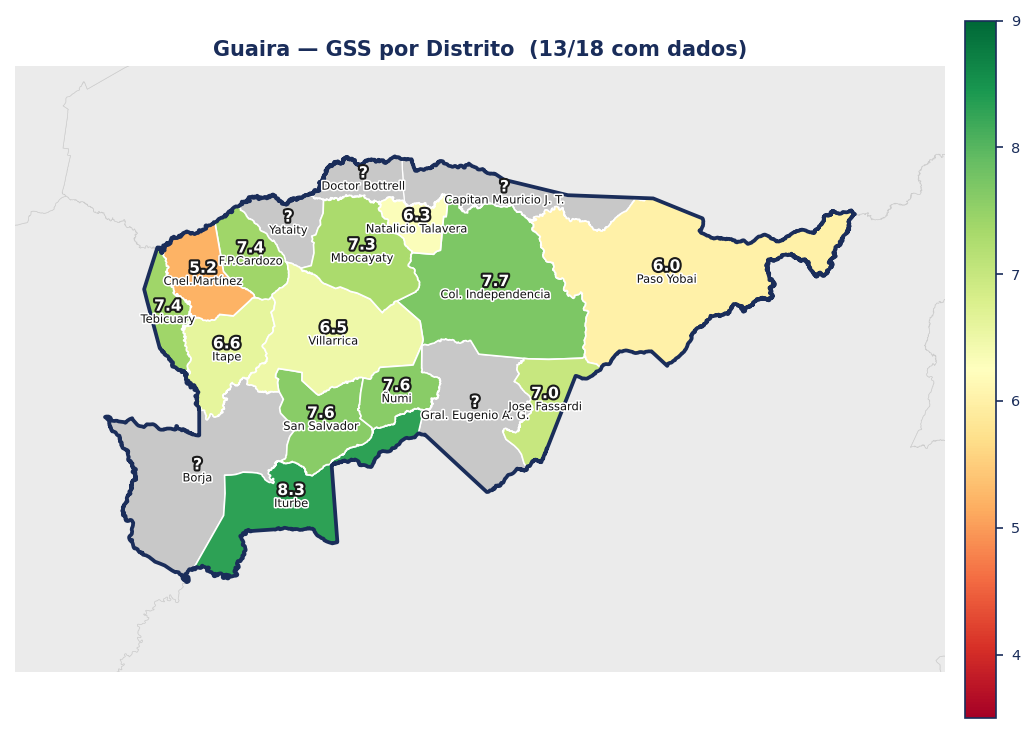
\includegraphics[width=\textwidth, height=0.55\textheight, keepaspectratio]{mapas/mapas_tematicos_dept_04_gss.png}
\caption{GSS (Global Safety Score) por distrito de Guaira. Verde = alta viabilidade · Vermelho = baixa viabilidade.}
\label{fig:gss-04}
\end{figure}

\vspace{0.5em}

\begin{figure}[htbp]
\centering
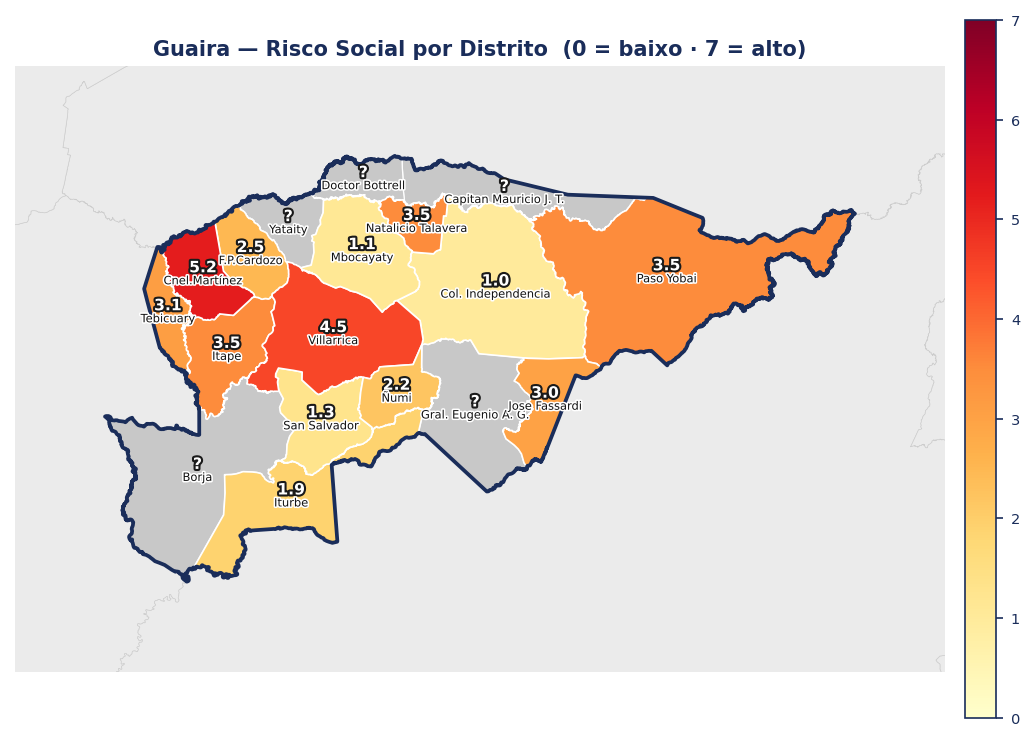
\includegraphics[width=\textwidth, height=0.55\textheight, keepaspectratio]{mapas/mapas_tematicos_dept_04_risco.png}
\caption{Risco social por distrito de Guaira. Amarelo = baixo risco · Vermelho = alto risco.}
\label{fig:risco-04}
\end{figure}

\clearpage

\begin{figure}[htbp]
\centering
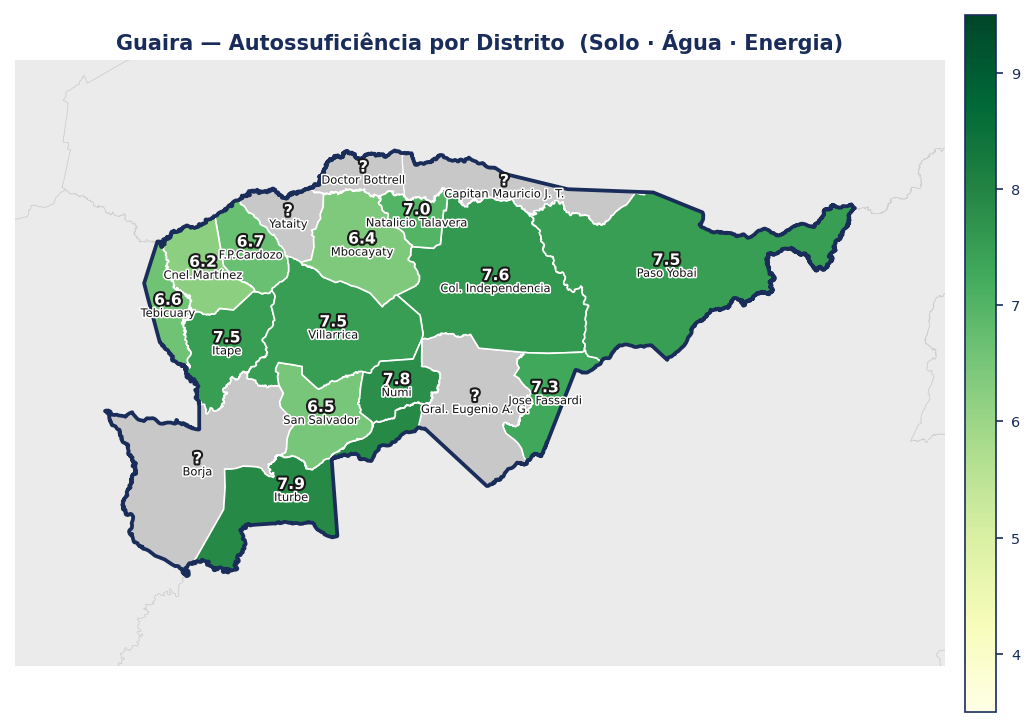
\includegraphics[width=\textwidth, height=0.55\textheight, keepaspectratio]{mapas/mapas_tematicos_dept_04_autosuf.png}
\caption{Autossuficiência por distrito de Guaira: solo, recursos hídricos e potencial energético. Branco = baixo · Verde escuro = alto.}
\label{fig:autosuf-04}
\end{figure}

\clearpage

\section{Guairá}

forte combinacao de turismo, servicos e agricultura.

\subsection{Ficha climática de Villarrica (capital
departamental)}

\textbf{Irradiância solar global --- (kWh/\allowbreak m²/\allowbreak dia):}


\begin{center}
\resizebox{\linewidth}{!}{%
{\renewcommand{\arraystretch}{1.2}%
\begin{tabular}{@{}c|c|c|c|c|c|c|c|c|c|c|c@{}}
\toprule
Jan & Fev & Mar & Abr & Mai & Jun & Jul & Ago & Set & Out & Nov & Dez \\
\midrule
6.74 & 6.20 & 5.50 & 4.48 & 3.35 & 2.88 & 3.21 & 3.96 & 4.59 & 5.43 &
6.43 & 6.81 \\
\bottomrule
\end{tabular}}%
}
\end{center}


Média anual: 4.96 kWh/\allowbreak m²/\allowbreak dia. Inclinação recomendada: 26° Norte (anual);
36° inverno; 16° verão.

\textbf{Precipitação --- (mm/\allowbreak mês):}


\begin{center}
\resizebox{\linewidth}{!}{%
{\renewcommand{\arraystretch}{1.2}%
\begin{tabular}{@{}c|c|c|c|c|c|c|c|c|c|c|c@{}}
\toprule
Jan & Fev & Mar & Abr & Mai & Jun & Jul & Ago & Set & Out & Nov & Dez \\
\midrule
131 & 136 & 131 & 152 & 172 & 90 & 75 & 52 & 92 & 187 & 190 & 166 \\
\bottomrule
\end{tabular}}%
}
\end{center}


Média anual: \textasciitilde1.573 mm/\allowbreak ano. Estação chuvosa Out-Mai; seca
Jun-Set.
\clearpage
\subsection*{Dados Departamentais}

\subsection*{Segurança Pública}

\begin{tabularx}{\linewidth}{lX}
\toprule
Indicador & Valor \\
\midrule
Taxa de homicídios (por 100k hab) & 1,74 (2022, fonte INE/Prosegur) \\
Crimes registrados (total/ano) & --- dados não desagregados publicamente \\
Número de comisarías & ~10 (estimativa departamental) \\
Índice segurança relativo & alto \\
\bottomrule
\end{tabularx}

Guairá apresenta uma das \textbf{menores taxas de homicídios do Paraguai}, com 1,74 por 100 mil habitantes em 2022, colocando-o entre os departamentos mais seguros do país. O Ministerio Público registra que Guairá responde por apenas \textbf{2\% das causas de homicídio doloso} nacional (2019--2024) --- proporção muito baixa e compatível com sua população de cerca de 3\% do total.

O departamento não possui fronteira internacional direta e está localizado na região centro-sul do Paraguai, distante das rotas principais de narcotráfico que afetam os departamentos fronteiriços com Brasil e Argentina. Villarrica, capital do departamento e terceira cidade mais importante do Paraguai, é conhecida por sua estabilidade social e tradição cultural.

A criminalidade é predominantemente patrimonial e de baixa intensidade. Não há registro significativo de atuação de crime organizado transnacional no departamento.

\subsection*{IDH e Desenvolvimento Humano}

\begin{tabularx}{\linewidth}{lX}
\toprule
Indicador & Valor \\
\midrule
IDH & 0,704 \\
Classificação IDH & alto \\
Ranking nacional (1=melhor) & 8/18 \\
Esperança de vida & 72,8 anos \\
Anos de escolaridade média & 8,2 anos \\
RNB per capita (USD PPA) & 8.700 \\
\bottomrule
\end{tabularx}

> Nota: IDH estimado com base no relatório PNUD 2020 e dados subnacionais. Guairá é um departamento de porte médio com economia diversificada (agricultura, indústria têxtil, turismo na Serra do Ybytyruzú). Estimativa baseada em perfil socioeconômico regional.

\begin{tabularx}{\linewidth}{lX}
\toprule
Indicador & Valor \\
\midrule
Taxa de pobreza total (\%) & 34,0\% \\
Taxa de pobreza extrema (\%) & 8,9\% \\
Índice de Gini & 0,455 \\
\bottomrule
\end{tabularx}

> Fonte: INE --- EPHC 2023. Pobreza multidimensional (IPM) de 25,48\% em 2023. Guairá apresenta alta pobreza apesar do IDH razoável, indicando desigualdade interna significativa.

\begin{tabularx}{\linewidth}{lX}
\toprule
Indicador & Valor \\
\midrule
Acesso a água potável (\%) & 76,5\% \\
Acesso a saneamento (\%) & 74,2\% \\
\bottomrule
\end{tabularx}

> Estimativa baseada em dados do Censo 2022. Villarrica, capital departamental, possui boa infraestrutura urbana, mas zonas rurais têm cobertura limitada.

Guairá é um departamento com IDH alto (0,704) e infraestrutura moderada. Villarrica, a capital, é uma cidade histórica e culturalmente vibrante, conhecida como "a Atenas do Paraguai" por sua tradição intelectual. O departamento tem presença de indústrias têxteis, agropecuária e o Parque Nacional Serra de San Rafael. Para brasileiros, destaca-se pela paisagem serrana (Serra do Ybytyruzú), clima agradável e custo de vida moderado. A taxa de pobreza de 34\% é alta e reflete desigualdades internas, mas a capital Villarrica oferece serviços adequados (hospitais regionais, universidades). Acesso a água (76,5\%) e saneamento (74,2\%) são medianos. Oportunidades em agronegócio, turismo ecológico e pequenas indústrias. Comunidade brasileira pequena mas presente.

\subsection*{Sistema Prisional}

{\small
{\small
\begin{tabularx}{\linewidth}{lXXXX}
\toprule
Nome & Município & Capacidade & População & Superlotação \\
\midrule
Penitenciaría Regional de Villarrica & Villarrica & 250 & ~480 & ~192\% \\
\bottomrule
\end{tabularx}
}
}

\begin{tabularx}{\linewidth}{lX}
\toprule
Indicador & Valor \\
\midrule
Total de estabelecimentos & 1 \\
Capacidade total (vagas) & ~250 \\
População carcerária total & ~480 \\
Taxa de superlotação & ~192\% \\
\% presos provisórios & ~66\% \\
\bottomrule
\end{tabularx}

A Penitenciaría Regional de Villarrica é o único estabelecimento penal formal do departamento de Guairá. Villarrica, capital departamental, é uma das cidades históricas do Paraguai e polo educacional e comercial do interior do país.

O presídio sofre de superlotação crônica, com detentos provenientes de todos os 17 municípios do departamento. O perfil de criminalidade local inclui crimes contra a propriedade, tráfico de entorpecentes em escala local e violência doméstica, sendo baixa a presença de crime organizado de grande porte.

O MNP registrou deficiências em assistência médica e jurídica no estabelecimento, com alta proporção de presos em prisão preventiva aguardando julgamento por longos períodos.

\textbf{Para imigrantes:} Guairá é um departamento com boa qualidade de vida relativa, forte tradição agrícola (soja, trigo, pecuária) e clima ameno. O ambiente prisional não representa risco direto para a população geral. A cidade de Villarrica tem infraestrutura urbana razoável e é considerada segura para instalação.

\subsection*{Recursos Hídricos Subterrâneos}

\begin{tabularx}{\linewidth}{lXXX}
\toprule
Aquífero & Cobertura no Dept. & Profundidade Média & Vazão Típica \\
\midrule
Guarani / Misiones (confinado) & ~60\% (porção leste) & 100--350 m & 20--80 m$^3$/h \\
Cristalino (fraturado, Pré-Cambriano) & ~40\% (porção oeste) & 30--100 m & 2--10 m$^3$/h \\
\bottomrule
\end{tabularx}

\begin{tabularx}{\linewidth}{lX}
\toprule
Parâmetro & Valor \\
\midrule
Profundidade média --- Cristalino (m) & 40--100 \\
Profundidade média --- Guarani (m) & 100--350 \\
Profundidade máxima recomendada (m) & 400 \\
Vazão típica (m$^3$/h) & 8--50 \\
Custo estimado perfuração (USD) & 3.000 -- 10.000 \\
Qualidade da água --- Cristalino & boa \\
Qualidade da água --- Guarani & boa a excelente \\
pH médio & 6,5--7,8 \\
Outorga necessária & sim \\
Órgão regulador & MADES --- DGPCRH \\
\bottomrule
\end{tabularx}

Guairá ocupa posição de transição entre o embasamento cristalino e as rochas sedimentares da Bacia do Paraná que hospedam o Aquífero Guarani. O extremo leste do departamento, próximo ao rio Paraná, tem boa cobertura do Guarani com profundidades acessíveis (100--200 m). A cidade de Villarrica (capital) se abastece parcialmente via poços artesianos e rede pública. A qualidade da água subterrânea é geralmente boa, com baixa mineralização. Guairá é reconhecido como área de recarga do Aquífero Guarani. O uso principal é abastecimento doméstico e irrigação agrícola.

Guairá é um departamento com terreno diversificado e produção agrícola expressiva. Para propriedades rurais no leste (Guarani acessível), poço de 100--200 m custa entre USD 3.500 e 8.000 e oferece excelente vazão para irrigação e uso doméstico. Na porção oeste/cristalina, poços de 40--80 m custam menos (USD 2.500--5.000), mas produtividade é mais variável. A rede pública em Villarrica é operada pelo SENASA. Para zonas rurais, poço próprio é a solução padrão.

\subsection*{Aptidão do Solo}

\begin{tabularx}{\linewidth}{lXX}
\toprule
Tipo de Solo & \% do Território & Características \\
\midrule
Ultissolos (Argissolos) & 45\% & Solos podzólicos vermelho-amarelados, textura areno-argilosa, fertilidade média-baixa \\
Oxissolos (Latossolos) & 25\% & Solos derivados de basalto no leste do departamento, maior fertilidade natural \\
Entissolos arenosos & 20\% & Solos arenosos de baixa retenção hídrica e fertilidade; suscetíveis à erosão \\
Aluviais / Inceptissolos & 10\% & Planícies fluviais do Rio Yhú e afluentes; fertilidade moderada \\
\bottomrule
\end{tabularx}

\begin{tabularx}{\linewidth}{lXX}
\toprule
Classe & \% Território & Uso Recomendado \\
\midrule
Lavoura intensiva & 20\% & Soja, milho, trigo (solos basálticos a leste) \\
Lavoura extensiva & 30\% & Mandioca, cana-de-açúcar, algodão, amendoim \\
Pastagem natural & 25\% & Pecuária extensiva \\
Floresta / reserva & 15\% & Matas ciliares, remanescentes de Mata Atlântica Interior \\
Sem aptidão agrícola & 10\% & Áreas urbanas, rochosas e degradadas \\
\bottomrule
\end{tabularx}

\begin{tabularx}{\linewidth}{lX}
\toprule
Parâmetro & Valor \\
\midrule
pH médio & 4,8 -- 5,8 \\
Fertilidade natural & baixa a média \\
Teor de matéria orgânica & baixo (>90\% dos solos cultivados deteriorados) \\
Necessidade de calcário & sim \\
\bottomrule
\end{tabularx}

Guairá tem potencial agrícola moderado, com as melhores áreas localizadas no leste do departamento (solos basálticos mais férteis). Comparativamente, os solos são inferiores aos Latossolos Roxos do Paraná, mas com manejo adequado (calagem, adubação, plantio direto) é possível obter produtividade razoável. O departamento é conhecido por suas cachoeiras (Saltos del Monday) e tem apelo turístico. Para grandes empreendimentos agrícolas mecanizados, Alto Paraná e Itapúa são mais indicados. A terra em Guairá é relativamente acessível para quem busca propriedades menores.

\subsection*{Terra Rural}

\begin{tabularx}{\linewidth}{lXXX}
\toprule
Tipo & Preço (USD/ha) & Faixa & Tendência \\
\midrule
Agrícola alta produtividade & 7.000 & 5.000 -- 10.000 & $\uparrow$ \\
Pastagem & 3.500 & 2.500 -- 5.000 & $\uparrow$ \\
Mata / reserva & 1.500 & 800 -- 2.500 & $\rightarrow$ \\
\bottomrule
\end{tabularx}

\begin{tabularx}{\linewidth}{lX}
\toprule
Parâmetro & Valor \\
\midrule
Valorização anual média (\%) & 7--9\% \\
Lote mínimo rural (ha) & 10 \\
Imposto territorial rural (\%) & 1\% sobre valor fiscal \\
Liquidez do mercado & média--alta \\
\bottomrule
\end{tabularx}

\begin{tabularx}{\linewidth}{lXXX}
\toprule
Indicador & Guairá (PY) & Paraná (BR) & São Paulo interior (BR) \\
\midrule
Terra agrícola (USD/ha) & 5.000--10.000 & 15.000--30.000 & 20.000--45.000 \\
Terra pastagem (USD/ha) & 2.500--5.000 & 6.000--12.000 & 8.000--18.000 \\
Custo relativo & ~35\% do PR & referência PR & referência SP \\
\bottomrule
\end{tabularx}

Guairá é vizinho do Paraná brasileiro e tem características geoclimáticas semelhantes. A diferença de preço de terra chega a 3--5x, sendo muito atrativo para produtores paranaenses que buscam expansão.

\subsection*{Mercado Imobiliário}

\textbf{Capital:} Villarrica

\begin{tabularx}{\linewidth}{lXX}
\toprule
Tipo & Preço (USD/m$^2$) & Aluguel (USD/mês) \\
\midrule
Apartamento 2 quartos & 600 -- 950 & 220 -- 420 \\
Casa 3 quartos & 500 -- 800 & 200 -- 380 \\
\bottomrule
\end{tabularx}

\begin{tabularx}{\linewidth}{lX}
\toprule
Parâmetro & Valor \\
\midrule
Valorização anual (\%) & 5--7\% \\
Disponibilidade de financiamento & boa (cooperativas ativas, BNF) \\
Bairros mais valorizados & Centro histórico, Barrio San Blas, Villa Florida \\
\bottomrule
\end{tabularx}

\textbf{Vale a pena comprar ou alugar?}
Villarrica é uma cidade histórica agradável (aprox. 70.000 hab.) com boa infraestrutura para cidade de interior paraguaio. É conhecida pela produção de artesanato, indústrias têxteis e vitivinicultura na Colônia Independencia (30 km). Para imigrantes com atividade na região, a compra é atrativa dado o baixo custo.

\textbf{Áreas recomendadas:}
O centro de Villarrica e as imediações da Ruta PY08 concentram a melhor oferta imobiliária do departamento, com boa proximidade a serviços, escolas e o comércio local. A Colônia Independencia (30 km) é opção interessante para quem busca ambiente rural com infraestrutura razoável.

\textbf{Armadilhas comuns:}
Parte dos imóveis urbanos mais antigos de Villarrica não possui conexão à rede de esgoto público --- verifique se o imóvel dispõe de fossa asséptica regular ou se há projeto de extensão da rede municipal para o local antes de fechar o negócio.

\subsection*{Cobertura Celular}

{\small
{\small
\begin{tabularx}{\linewidth}{lXXXXX}
\toprule
Operadora & 2G & 3G & 4G & 5G & Cobertura Pop. \\
\midrule
Tigo & 88\% & 78\% & 68\% & --- & 82\% \\
Personal/Claro & 80\% & 70\% & 60\% & --- & 75\% \\
VOX & 50\% & 35\% & 20\% & --- & 42\% \\
\bottomrule
\end{tabularx}
}
}

> \textbf{Nota:} Guairá tem cobertura concentrada em Villarrica (capital, ~120k hab.) e ao longo da Ruta 8 (Coronel Oviedo--Encarnación). Interior serrano e municípios menores têm 3G predominante.

\begin{tabularx}{\linewidth}{lX}
\toprule
Parâmetro & Valor \\
\midrule
Melhor operadora rural & Tigo \\
Velocidade 4G média (Mbps) & 18--35 \\
Áreas sem cobertura & Zonas serranas do leste, áreas de mata \\
Sinal em propriedade rural & moderado \\
\bottomrule
\end{tabularx}

\begin{tabularx}{\linewidth}{lXXX}
\toprule
Plano & Operadora & USD/mês & Dados \\
\midrule
Pré-pago básico (7 dias) & Tigo & ~2,50 & 3 GB \\
Pré-pago intermediário (30 dias) & Personal & ~5,00 & 8 GB \\
Pós-pago entrada & Tigo & ~12,00 & 15 GB + chamadas \\
Pós-pago intermediário & Personal/Claro & ~18,00 & 30 GB + chamadas \\
\bottomrule
\end{tabularx}

\subsection*{Internet}

\begin{tabularx}{\linewidth}{lX}
\toprule
Indicador & Valor \\
\midrule
\% população com internet & ~65\% \\
\% com banda larga fixa & ~22\% dos domicílios \\
Velocidade média download (Mbps) & 25--60 (urbano) / 5--15 (rural) \\
Velocidade média upload (Mbps) & 8--20 (urbano) \\
\bottomrule
\end{tabularx}

\begin{tabularx}{\linewidth}{lXX}
\toprule
Tecnologia & Disponibilidade & Velocidade Típica \\
\midrule
Fibra ótica (FTTH) & Villarrica e municípios principais & 50--300 Mbps \\
Cabo HFC & Villarrica & 30--150 Mbps \\
Rádio/Wireless & Amplo no departamento & 5--50 Mbps \\
ADSL (Copaco) & Interior com rede legada & 2--10 Mbps \\
Satélite (Starlink) & Todo o departamento & 50--200 Mbps \\
\bottomrule
\end{tabularx}

\begin{tabularx}{\linewidth}{lXXX}
\toprule
Provedor & Tecnologia & Área de cobertura & Preço ref. (USD/mês) \\
\midrule
Tigo & Fibra/HFC/Rádio & Villarrica + municípios & 18--50 \\
Claro/Personal & Fibra/Rádio & Villarrica & 15--45 \\
Copaco & ADSL/Rádio & Todo o departamento (rede legada) & 10--28 \\
Starlink & Satélite LEO & Todo o departamento & ~44 + equip. ~370 \\
\bottomrule
\end{tabularx}

A cobertura rural de Guairá é \textbf{moderada}. Villarrica e cidades ao longo da Ruta 8 têm boa conectividade. O interior serrano, especialmente em áreas com topografia acidentada, tem cobertura mais limitada:

\clearpage
\newpage
\secaoDiagnostico{Borja}{\mapaDistrito{0402}}{Borja é um município rural tranquilo no sudoeste do departamento de
Guairá, situado a aproximadamente 30~km de Villarrica pela Ruta~8.
Com cerca de 8.000 habitantes distribuídos em colinas suaves e
campos férteis, combina baixíssima densidade demográfica, forte
tradição de agricultura familiar e clima subtropical ameno. Para o
imigrante brasileiro que prioriza discrição, custo de vida reduzido
e conexão direta com a terra, Borja representa uma escolha sólida
e acessível no coração de Guairá.

\subsubsection{Recomendação Técnica}

Recomendado para perfis agropecuários e famílias que valorizam
sossego rural com razoável acesso à capital departamental. O GSS
de 6.8 reflete segurança institucional elevada, bom ambiente social
e produtividade agrícola consistente, com desconto pela ausência de
banco local e pelo abastecimento de serviços concentrado em
Villarrica. Referência atual de score: GSS 6.8.

}
\begin{table}[ht!]
\small \begin{tabular}{p{3.0cm}p{0.8cm}p{6.0cm}} \toprule
\textbf{Critério} & \textbf{Nota} & \textbf{Justificativa} \\ \midrule
A - Ameaças Estratégicas & 8.0 & Interior distante de fronteiras e eixos de conflito; sem alvos estratégicos relevantes \\
B - Risco Social & 7.0 & Ambiente rural pacífico; criminalidade limitada a abigeato esporádico \\
C - Riscos Naturais & 6.5 & Geologia estável em colinas; risco moderado de alagamentos em baixadas \\
D - Autossuficiência & 5.5 & Boa produção agrícola (soja, milho, pecuária), mas sem banco local e serviços técnicos limitados \\
E - Institucional & 6.5 & Municipalidade funcional; serviços básicos presentes; referência hospitalar em Villarrica \\
\midrule
 \textbf{GSS FINAL} & \textbf{6.8} & \textbf{Seguro (Município rural recomendado para perfis agropecuários que buscam tranquilidade e custo baixo).} \\ \bottomrule
 \end{tabular}
\end{table}
\subsubsection{Vulnerabilidades e
Mitigação}\label{vuln-Borja-vulnerabilidades-e-mitigacao}

\begin{itemize}
\tightlist
\item
  \textbf{Ausência de Banco Local:} Toda movimentação financeira exige
  deslocamento até Villarrica (\textasciitilde 30~km)
  (Mitigação: manter reserva em espécie e usar aplicativos bancários
  digitais via 4G Tigo).
\item
  \textbf{Serviços de Saúde Limitados:} O posto de saúde local cobre
  apenas atenção primária; emergências seguem para Villarrica
  (Mitigação: plano de saúde privado e kit de primeiros socorros
  completo em domicílio).
\item
  \textbf{Risco de Alagamento em Baixadas:} Áreas próximas a arroios
  tributários podem sofrer transbordamentos em períodos de El Niño
  intenso (Mitigação: construção em cotas acima de 160~m e
  mapeamento prévio dos cursos d'água).
\item
  \textbf{Dependência de Serviços em Villarrica:} Comércio especializado,
  ensino médio completo e serviços técnicos concentram-se na capital
  departamental (Mitigação: acesso facilitado pela Ruta~8 asfaltada).
\end{itemize}

\subsubsection{Dossiê de Campo}\label{dossie-Borja-dossie-de-campo}
\begin{description}[style=nextline,leftmargin=0.5cm,font=\bfseries]
\item[Coordenadas]  25°54'S 56°23'W (centro urbano estimado).
\item[Topografia]  Colinas suaves com vales férteis; altitude média \textasciitilde 180~m. Relevo ondulado sem impedimentos à mecanização agrícola. Risco sísmico desprezível.
\item[Alvos Estratégicos]  Nenhum de relevância estratégica elevada; silos de grãos de pequeno porte e frigoríficos locais representam infraestrutura econômica, não alvo militar.
\item[Fallout]  Ventos predominantes de Leste e Sudeste durante a maior parte do ano; Norte-Nordeste no verão. Baixíssimo risco de fallout direto pela distância de qualquer instalação industrial crítica.
\item[População]  \textasciitilde 8.000 habitantes (estimativa Censo 2022). Perfil predominantemente rural (\textgreater 80\%), com forte presença de agricultores familiares.
\item[Densidade]  \textasciitilde 12--16 hab/\allowbreak km² (baixíssima densidade, favorecendo privacidade e isolamento voluntário).
\item[Vias de Acesso]  Acesso principal pela Ruta~8 (Villarrica--Coronel Oviedo), com ramal asfaltado local. Estradas vicinais de terra exigem veículo 4x4 após chuvas intensas.
\item[Serviços]  Posto de saúde (USF); escola primária e ensino médio parcial; feria semanal; sem banco local (caixas eletrônicos em Villarrica). Farmácia local disponível.
\item[Custo de Vida]  Muito baixo; alimentos produzidos localmente; aluguel rural estimado em USD 100--200/\allowbreak mês; terra mais barata que a média departamental.
\item[Preço da Terra]  USD 2.000--5.000/\allowbreak ha (campos de pastagem e lavoura); USD 8.000--12.000/\allowbreak ha (terras mecanizadas em posição privilegiada).
\item[Hidrologia]  Abastecimento pelo Aquífero Guarani (poços artesianos com profundidade 100--250~m). Arroios tributários do Tebicuary-mí em zonas baixas com risco ocasional de alagamento.
\item[Clima]  Subtropical úmido (Cfa/Cwa); temperatura média anual \textasciitilde 22°C; precipitação \textasciitilde 1.580~mm/\allowbreak ano; verões quentes (até 36°C) e invernos amenos com eventuais frentes frias do Sul.
\item[Energia]  Rede da ANDE (Itaipu); cobertura elétrica em área urbana e ao longo das vias principais; zonas rurais distantes podem ter instabilidades. Solar fotovoltaico altamente viável (média 4,9~kWh/m²/dia).
\item[Água]  Excelente via Aquífero Guarani; poços artesianos produtivos com boa qualidade química. Arroios disponíveis para uso agrícola com filtragem.
\item[Qualidade do Solo]  Latossolos vermelhos (Terra Roja) e solos podzólicos nas encostas; pH levemente ácido (5,0--5,5); boa fertilidade natural para soja, milho, mandioca e pastagens.
\item[Recursos Locais]  Soja, milho, pecuária de corte e leiteira; suinocultura; mel; mandioca. Feria semanal com produtos frescos. Potencial para horta familiar e policultura de subsistência.
\item[Segurança]  Zona rural extremamente pacífica. Guairá registra uma das menores taxas de homicídios do Paraguai (\textasciitilde 1,74/\allowbreak 100k hab em 2022). Ocorrências limitam-se a abigeato esporádico.
\item[Leis e Restrições]  Município consolidado no interior do país; sem restrição de fronteira para estrangeiros. Titularidade plena disponível para brasileiros em terras privadas regularizadas.
\end{description}
\textbf{Fonte climática:} NASA POWER Climatology API (período 2001--2020)

\textbf{Fonte luminosa:} estimativa World Atlas of Light Pollution

\paragraph{Irradiação Solar
(kWh/\allowbreak m²/\allowbreak dia)}


\begin{center}
\resizebox{\linewidth}{!}{%
{\renewcommand{\arraystretch}{1.2}%
\begin{tabular}{@{}c|c|c|c|c|c|c|c|c|c|c|c|c@{}}
\toprule
Jan & Fev & Mar & Abr & Mai & Jun & Jul & Ago & Set & Out & Nov & Dez & Média \\
\midrule
6.74 & 6.20 & 5.50 & 4.48 & 3.35 & 2.88 & 3.21 & 3.96 & 4.59 & 5.43 &
6.43 & 6.81 & \textbf{4.96} \\
\bottomrule
\end{tabular}}%
}
\end{center}


\textbf{Inclinação solar recomendada:} 26° N (anual) · 36° N (inverno
jun-ago) · 16° N (verão nov-jan)

\paragraph{Precipitação (mm/\allowbreak mês)}


\begin{center}
\resizebox{\linewidth}{!}{%
{\renewcommand{\arraystretch}{1.2}%
\begin{tabular}{@{}c|c|c|c|c|c|c|c|c|c|c|c|c@{}}
\toprule
Jan & Fev & Mar & Abr & Mai & Jun & Jul & Ago & Set & Out & Nov & Dez & Total/\allowbreak ano \\
\midrule
135 & 130 & 133 & 155 & 168 & 92 & 77 & 60 & 92 & 188 & 189 & 161 &
\textbf{1580 mm} \\
\bottomrule
\end{tabular}}%
}
\end{center}


\paragraph{Poluição Luminosa}

\begin{longtable}[]{@{}ll@{}}
\toprule\noalign{}
Parâmetro & Valor \\
\midrule\noalign{}
\endhead
\bottomrule\noalign{}
\endlastfoot
Escala Bortle & 3--4 --- Céu rural escuro \\
Radiância artificial & \textasciitilde 2,0 nW/\allowbreak cm²/\allowbreak sr \\
\end{longtable}

\paragraph{Solo (SoilGrids 2.0, média ponderada 0--30 cm)}

\begin{longtable}[]{@{}ll@{}}
\toprule\noalign{}
Parâmetro & Valor \\
\midrule\noalign{}
\endhead
\bottomrule\noalign{}
\endlastfoot
pH (H$_2$O) & 5,10 \\
Carbono orgânico (SOC) & 16,2 g/\allowbreak kg \\
Argila & 24,5\% \\
Areia & 49,0\% \\
Silte (calc.) & 26,5\% \\
Densidade aparente & 1,36 g/\allowbreak cm³ \\
\textbf{Aptidão agrícola} & \textbf{Boa (soja, milho, pastagens)} \\
\end{longtable}

\subsubsection{Indicadores Sociais}

\textbf{Fontes:} PNUD 2020, INE\footnote{\fineINE} Censo 2022, INE\footnote{\fineINE} EPHC 2023, Ministerio
Público 2024\\
\textbf{Nota:} Valores marcados como \emph{(dept.)} referem-se ao
departamento de Guairá; valores \emph{(dist.)} são específicos deste
distrito. Dados marcados \emph{(est.)} são estimativas.

\begin{longtable}[]{@{}
  >{\raggedright\arraybackslash}p{(\linewidth - 4\tabcolsep) * \real{0.4231}}
  >{\raggedright\arraybackslash}p{(\linewidth - 4\tabcolsep) * \real{0.2692}}
  >{\raggedright\arraybackslash}p{(\linewidth - 4\tabcolsep) * \real{0.3077}}@{}}
\toprule\noalign{}
\begin{minipage}[b]{\linewidth}\raggedright
Indicador
\end{minipage} & \begin{minipage}[b]{\linewidth}\raggedright
Valor
\end{minipage} & \begin{minipage}[b]{\linewidth}\raggedright
Âmbito
\end{minipage} \\
\midrule\noalign{}
\endhead
\bottomrule\noalign{}
\endlastfoot
IDH (2020) & 0,704 & dept. \\
Ranking IDH nacional & 8/\allowbreak 18 & dept. \\
Esperança de vida & 72,8 anos & dept. \\
Escolaridade média & 7,4 anos & dist. (est.) \\
RNB per capita (USD PPA) & 8.700 & dept. \\
Pobreza monetária (\%) & 34,0\% & dept. \\
Pobreza extrema (\%) & 8,9\% & dept. \\
Índice de Gini & 0,455 & dept. \\
Acesso a água potável (\%) & 76,5\% & dept. \\
Acesso a saneamento (\%) & 74,2\% & dept. \\
Taxa de homicídios (est., /\allowbreak 100k hab) & 1,74 (2022, fonte INE\footnote{\fineINE}/\allowbreak Prosegur) & dept. \\
Índice de segurança & alto & dept. \\
População (Censo 2022) & \textasciitilde 8.000 habitantes & dist. (est.) \\
Idade mediana & N/\allowbreak D & dist. \\
Taxa de fecundidade & N/\allowbreak D & dist. \\
\end{longtable}

\subsubsection{Combustível}

\textbf{Referência:} PETROPAR /\allowbreak  postos locais (2024) \textbf{Tipo de
localidade:} Interior

\begin{longtable}[]{@{}lll@{}}
\toprule\noalign{}
Combustível & USD/\allowbreak litro & Gs/\allowbreak litro (aprox.) \\
\midrule\noalign{}
\endhead
\bottomrule\noalign{}
\endlastfoot
Gasolina 93 oct & 0,97 & 7.178 \\
Gasolina 97 oct (premium) & 1,07 & 7.918 \\
Diesel & 0,90 & 6.660 \\
\end{longtable}

\begin{quote}
Preços podem variar ±5\% conforme posto e sazonalidade. Sem posto
em Borja, recomenda-se abastecer em Villarrica ou ao longo da Ruta~8.
\end{quote}

\subsubsection{Cobertura Celular}

\textbf{Fonte:} CONATEL PY /\allowbreak  operadoras (2024)

\begin{longtable}[]{@{}ll@{}}
\toprule\noalign{}
Parâmetro & Valor \\
\midrule\noalign{}
\endhead
\bottomrule\noalign{}
\endlastfoot
Cobertura 4G população (dept.) & 87\% \\
Cobertura 4G área rural & 70\% \\
Melhor operadora & Tigo \\
Qualidade rural & boa (4G Tigo cobrindo a sede e principais vias) \\
\end{longtable}

\begin{quote}
Para zonas rurais afastadas da sede municipal, recomenda-se chip Tigo
como principal e Personal como backup. Starlink disponível como
alternativa de alta velocidade.
\end{quote}

\subsubsection{Internet}

\textbf{Fonte:} CONATEL /\allowbreak  Speedtest Ookla (2024)

\begin{longtable}[]{@{}ll@{}}
\toprule\noalign{}
Parâmetro & Valor \\
\midrule\noalign{}
\endhead
\bottomrule\noalign{}
\endlastfoot
Velocidade média download & 40--50 Mbps (área urbana) \\
Domicílios com internet (dept.) & 60\% \\
Tecnologia predominante & rádio / 4G fixo \\
Opção rural & Starlink disponível (\textasciitilde USD 44/\allowbreak mês) \\
\end{longtable}

\subsubsection{Mercado Imobiliário e Terra Rural}

\textbf{Fonte:} INDERT /\allowbreak  Clasificados.com.py (2024)

\begin{longtable}[]{@{}ll@{}}
\toprule\noalign{}
Tipo & Referência \\
\midrule\noalign{}
\endhead
\bottomrule\noalign{}
\endlastfoot
Terra agrícola (soja/milho) (USD/\allowbreak ha) & 3.500--5.500 \\
Terra de pastagem (USD/\allowbreak ha) & 2.000--3.500 \\
Imóvel urbano (USD/\allowbreak m²) & 300--500 \\
Aluguel casa rural (USD/\allowbreak mês) & 100--200 \\
\end{longtable}

\begin{quote}
Valores sensivelmente abaixo da média departamental por ser município
pequeno sem polo industrial. Boa relação custo-benefício para
estabelecimentos rurais de médio porte.
\end{quote}

\subsubsection{Saúde}

\textbf{Fonte:} MSPBS /\allowbreak  IPS Paraguay (2024--2026), consolidação
departamental e proxy local

\begin{longtable}[]{@{}ll@{}}
\toprule\noalign{}
Serviço & Disponibilidade \\
\midrule\noalign{}
\endhead
\bottomrule\noalign{}
\endlastfoot
USF /\allowbreak  Posto de Saúde & sim \\
Hospital Regional & não (referência em Villarrica) \\
IPS (seguro social) & não \\
Farmácia & sim (farmácia local) \\
Distância ao hospital de referência & \textasciitilde 30~km (Villarrica) \\
\end{longtable}

\textbf{Principais estabelecimentos:} USF local para atenção primária;
Hospital Regional de Villarrica como referência para média e alta
complexidade.

\textbf{Observação para imigrantes:} Atenção primária disponível
localmente; casos de maior complexidade requerem deslocamento a
Villarrica (\textasciitilde 30~min pela Ruta~8). Cobertura privada fortemente
recomendada para especialidades e emergências cirúrgicas.
\newpage
\secaoDiagnostico{Capitan Mauricio Jose Troche}{\mapaDistrito{0403}}{Capitán Mauricio José Troche é um município rural tranquilo no nordeste
do departamento de Guairá, próximo à Serra de San Joaquín. Com cerca de
9.000 habitantes distribuídos em colinas com mata ciliar, combina
economia agropecuária sólida (soja, milho, pecuária) com baixíssima
densidade demográfica e acesso ao Aquífero Guarani. Situado a
\textasciitilde 180~km de Assunção pela Ruta~8, o município homenageia
o herói da Guerra da Tríplice Aliança Capitán Mauricio José Troche.
Para o imigrante que prioriza discrição, custo de vida baixo e
conexão com a terra, Troche representa uma escolha sólida no interior
de Guairá.

\subsubsection{Recomendação Técnica}

Recomendado para perfis agropecuários e famílias que valorizam sossego
rural com acesso razoável à capital departamental. O GSS de 7.3 reflete
segurança institucional elevada, bom ambiente social e produtividade
agrícola consistente em região de colinas com boa disponibilidade
hídrica. Referência atual de score: GSS 7.3.

}
\begin{table}[ht!]
\small \begin{tabular}{p{3.0cm}p{0.8cm}p{6.0cm}} \toprule
\textbf{Critério} & \textbf{Nota} & \textbf{Justificativa} \\ \midrule
A - Ameaças Estratégicas & 8.0 & Interior distante de fronteiras e eixos de conflito; sem alvos estratégicos relevantes \\
B - Risco Social & 7.5 & Ambiente rural pacífico; criminalidade muito baixa; forte coesão comunitária agropecuária \\
C - Riscos Naturais & 7.0 & Colinas com geologia estável; risco moderado de alagamentos pontuais em baixadas \\
D - Autossuficiência & 6.5 & Boa produção agropecuária (soja, milho, pecuária), mas serviços especializados em Villarrica \\
E - Institucional & 7.0 & Municipalidade funcional; serviços básicos presentes; referência hospitalar em Villarrica \\
\midrule
 \textbf{GSS FINAL} & \textbf{7.3} & \textbf{Seguro (Município rural recomendado para perfis agropecuários que buscam tranquilidade e custo baixo).} \\ \bottomrule
 \end{tabular}
\end{table}
\subsubsection{Vulnerabilidades e Mitigação}\label{vuln-Capitan_Mauricio_Jose_Troche-vulnerabilidades-e-mitigacao}

\begin{itemize}
\tightlist
\item
  \textbf{Ausência de Banco Local:} Movimentação financeira exige
  deslocamento até Villarrica ou Coronel Oviedo
  (Mitigação: manter reserva em espécie e usar aplicativos bancários
  digitais via 4G Tigo).
\item
  \textbf{Serviços de Saúde Limitados:} O posto de saúde local cobre
  apenas atenção primária; emergências seguem para Villarrica
  (Mitigação: plano de saúde privado e kit de primeiros socorros
  completo em domicílio).
\item
  \textbf{Risco de Alagamento em Baixadas:} Áreas próximas a arroios
  tributários podem sofrer transbordamentos em períodos de El Niño
  intenso (Mitigação: construção em cotas elevadas nas colinas e
  mapeamento prévio dos cursos d'água).
\item
  \textbf{Cobertura Celular Moderada:} 4G disponível na sede, mas com
  cobertura irregular em zonas rurais afastadas
  (Mitigação: chip Tigo como principal e Starlink como backup em
  propriedades rurais remotas).
\end{itemize}

\subsubsection{Dossiê de Campo}\label{dossie-Capitan_Mauricio_Jose_Troche-dossie-de-campo}
\begin{description}[style=nextline,leftmargin=0.5cm,font=\bfseries]
\item[Coordenadas]  25°29'S 56°07'W (centro urbano estimado).
\item[Topografia]  Região de colinas com mata ciliar; altitude média \textasciitilde 200--250~m. Relevo ondulado próximo à Serra de San Joaquín. Risco sísmico desprezível.
\item[Alvos Estratégicos]  Nenhum de relevância estratégica elevada; silos de grãos de pequeno porte representam infraestrutura econômica local, não alvo militar.
\item[Fallout]  Ventos predominantes de Leste e Sudeste durante a maior parte do ano; Norte-Nordeste no verão. Baixíssimo risco de fallout direto pela distância de qualquer instalação industrial crítica.
\item[População]  \textasciitilde 9.000 habitantes (estimativa Censo 2022). Perfil predominantemente rural (\textgreater 80\%), com forte presença de agricultores e pecuaristas.
\item[Densidade]  \textasciitilde 15--20 hab/\allowbreak km² (baixa densidade, favorecendo privacidade e isolamento voluntário).
\item[Vias de Acesso]  Acesso pela Ruta~8 (Villarrica--Coronel Oviedo) com ramal local; \textasciitilde 180~km de Assunção. Estradas vicinais de terra exigem veículo 4x4 após chuvas intensas.
\item[Serviços]  Posto de saúde (USF); escola primária e ensino médio parcial; feria semanal; sem banco local (caixas eletrônicos em Villarrica ou Coronel Oviedo). Farmácia local disponível.
\item[Custo de Vida]  Muito baixo; alimentos produzidos localmente; aluguel rural estimado em USD 100--200/\allowbreak mês; terra abaixo da média departamental.
\item[Preço da Terra]  USD 2.500--5.500/\allowbreak ha (campos de pastagem e lavoura); USD 6.000--9.000/\allowbreak ha (terras mecanizadas em posição privilegiada).
\item[Hidrologia]  Abastecimento pelo Aquífero Guarani (poços artesianos com profundidade 100--250~m). Arroios tributários em zonas baixas com risco ocasional de alagamento.
\item[Clima]  Subtropical úmido (Cfa/Cwa); temperatura média anual \textasciitilde 22°C; precipitação \textasciitilde 1.580~mm/\allowbreak ano; verões quentes (até 36°C) e invernos amenos com eventuais frentes frias do Sul.
\item[Energia]  Rede da ANDE (Itaipu); cobertura elétrica na área urbana e ao longo das vias principais; zonas rurais distantes podem ter instabilidades. Solar fotovoltaico altamente viável (média \textasciitilde 4,9~kWh/m²/dia).
\item[Água]  Excelente via Aquífero Guarani; poços artesianos produtivos com boa qualidade química. Arroios disponíveis para uso agrícola com filtragem.
\item[Qualidade do Solo]  Latossolos vermelhos (Terra Roja) e solos podzólicos nas encostas; pH levemente ácido (5,0--5,5); boa fertilidade natural para soja, milho, mandioca e pastagens.
\item[Recursos Locais]  Soja, milho, pecuária de corte e leiteira; mandioca; mel. Feria semanal com produtos frescos. Potencial para horta familiar e policultura de subsistência.
\item[Segurança]  Zona rural extremamente pacífica. Guairá registra uma das menores taxas de homicídios do Paraguai (\textasciitilde 1,74/\allowbreak 100k hab em 2022). Ocorrências limitam-se a abigeato esporádico.
\item[Leis e Restrições]  Município consolidado no interior do país; sem restrição de fronteira para estrangeiros. Titularidade plena disponível para brasileiros em terras privadas regularizadas.
\end{description}
\textbf{Fonte climática:} NASA POWER Climatology API (período 2001--2020)

\textbf{Fonte luminosa:} estimativa World Atlas of Light Pollution

\paragraph{Irradiação Solar
(kWh/\allowbreak m²/\allowbreak dia)}


\begin{center}
\resizebox{\linewidth}{!}{%
{\renewcommand{\arraystretch}{1.2}%
\begin{tabular}{@{}c|c|c|c|c|c|c|c|c|c|c|c|c@{}}
\toprule
Jan & Fev & Mar & Abr & Mai & Jun & Jul & Ago & Set & Out & Nov & Dez & Média \\
\midrule
6.74 & 6.20 & 5.50 & 4.48 & 3.35 & 2.88 & 3.21 & 3.96 & 4.59 & 5.43 &
6.43 & 6.81 & \textbf{4.96} \\
\bottomrule
\end{tabular}}%
}
\end{center}


\textbf{Inclinação solar recomendada:} 26° N (anual) · 36° N (inverno
jun-ago) · 16° N (verão nov-jan)

\paragraph{Precipitação (mm/\allowbreak mês)}


\begin{center}
\resizebox{\linewidth}{!}{%
{\renewcommand{\arraystretch}{1.2}%
\begin{tabular}{@{}c|c|c|c|c|c|c|c|c|c|c|c|c@{}}
\toprule
Jan & Fev & Mar & Abr & Mai & Jun & Jul & Ago & Set & Out & Nov & Dez & Total/\allowbreak ano \\
\midrule
135 & 130 & 133 & 155 & 168 & 92 & 77 & 60 & 92 & 188 & 189 & 161 &
\textbf{1580 mm} \\
\bottomrule
\end{tabular}}%
}
\end{center}


\paragraph{Poluição Luminosa}

\begin{longtable}[]{@{}ll@{}}
\toprule\noalign{}
Parâmetro & Valor \\
\midrule\noalign{}
\endhead
\bottomrule\noalign{}
\endlastfoot
Escala Bortle & 3--4 --- Céu rural escuro \\
Radiância artificial & \textasciitilde 2,0 nW/\allowbreak cm²/\allowbreak sr \\
\end{longtable}

\paragraph{Solo (SoilGrids 2.0, média ponderada 0--30 cm)}

\begin{longtable}[]{@{}ll@{}}
\toprule\noalign{}
Parâmetro & Valor \\
\midrule\noalign{}
\endhead
\bottomrule\noalign{}
\endlastfoot
pH (H$_2$O) & 5,10 \\
Carbono orgânico (SOC) & 16,5 g/\allowbreak kg \\
Argila & 25,0\% \\
Areia & 49,5\% \\
Silte (calc.) & 25,5\% \\
Densidade aparente & 1,34 g/\allowbreak cm³ \\
\textbf{Aptidão agrícola} & \textbf{Boa (soja, milho, pastagens)} \\
\end{longtable}

\subsubsection{Indicadores Sociais}

\textbf{Fontes:} PNUD 2020, INE\footnote{\fineINE} Censo 2022, INE\footnote{\fineINE} EPHC 2023, Ministerio
Público 2024\\
\textbf{Nota:} Valores marcados como \emph{(dept.)} referem-se ao
departamento de Guairá; valores \emph{(dist.)} são específicos deste
distrito. Dados marcados \emph{(est.)} são estimativas.

\begin{longtable}[]{@{}
  >{\raggedright\arraybackslash}p{(\linewidth - 4\tabcolsep) * \real{0.4231}}
  >{\raggedright\arraybackslash}p{(\linewidth - 4\tabcolsep) * \real{0.2692}}
  >{\raggedright\arraybackslash}p{(\linewidth - 4\tabcolsep) * \real{0.3077}}@{}}
\toprule\noalign{}
\begin{minipage}[b]{\linewidth}\raggedright
Indicador
\end{minipage} & \begin{minipage}[b]{\linewidth}\raggedright
Valor
\end{minipage} & \begin{minipage}[b]{\linewidth}\raggedright
Âmbito
\end{minipage} \\
\midrule\noalign{}
\endhead
\bottomrule\noalign{}
\endlastfoot
IDH (2020) & 0,704 & dept. \\
Ranking IDH nacional & 8/\allowbreak 18 & dept. \\
Esperança de vida & 72,8 anos & dept. \\
Escolaridade média & 7,4 anos & dist. (est.) \\
RNB per capita (USD PPA) & 8.700 & dept. \\
Pobreza monetária (\%) & 34,0\% & dept. \\
Pobreza extrema (\%) & 8,9\% & dept. \\
Índice de Gini & 0,455 & dept. \\
Acesso a água potável (\%) & 76,5\% & dept. \\
Acesso a saneamento (\%) & 74,2\% & dept. \\
Taxa de homicídios (est., /\allowbreak 100k hab) & 1,74 (2022, fonte INE\footnote{\fineINE}/\allowbreak Prosegur) & dept. \\
Índice de segurança & alto & dept. \\
População (Censo 2022) & \textasciitilde 9.000 habitantes & dist. (est.) \\
Idade mediana & N/\allowbreak D & dist. \\
Taxa de fecundidade & N/\allowbreak D & dist. \\
\end{longtable}

\subsubsection{Combustível}

\textbf{Referência:} PETROPAR /\allowbreak  postos locais (2024) \textbf{Tipo de
localidade:} Interior

\begin{longtable}[]{@{}lll@{}}
\toprule\noalign{}
Combustível & USD/\allowbreak litro & Gs/\allowbreak litro (aprox.) \\
\midrule\noalign{}
\endhead
\bottomrule\noalign{}
\endlastfoot
Gasolina 93 oct & 0,97 & 7.178 \\
Gasolina 97 oct (premium) & 1,07 & 7.918 \\
Diesel & 0,90 & 6.660 \\
\end{longtable}

\begin{quote}
Preços podem variar ±5\% conforme posto e sazonalidade. Sem posto
local, recomenda-se abastecer em Villarrica ou ao longo da Ruta~8.
\end{quote}

\subsubsection{Cobertura Celular}

\textbf{Fonte:} CONATEL PY /\allowbreak  operadoras (2024)

\begin{longtable}[]{@{}ll@{}}
\toprule\noalign{}
Parâmetro & Valor \\
\midrule\noalign{}
\endhead
\bottomrule\noalign{}
\endlastfoot
Cobertura 4G população (dept.) & 87\% \\
Cobertura 4G área rural & 60--70\% \\
Melhor operadora & Tigo \\
Qualidade rural & moderada (4G Tigo cobrindo sede e principais vias) \\
\end{longtable}

\begin{quote}
Para zonas rurais afastadas da sede municipal, recomenda-se chip Tigo
como principal e Personal como backup. Starlink disponível como
alternativa de alta velocidade em propriedades remotas.
\end{quote}

\subsubsection{Internet}

\textbf{Fonte:} CONATEL /\allowbreak  Speedtest Ookla (2024)

\begin{longtable}[]{@{}ll@{}}
\toprule\noalign{}
Parâmetro & Valor \\
\midrule\noalign{}
\endhead
\bottomrule\noalign{}
\endlastfoot
Velocidade média download & 30--45 Mbps (área urbana) \\
Domicílios com internet (dept.) & 60\% \\
Tecnologia predominante & rádio / 4G fixo \\
Opção rural & Starlink disponível (\textasciitilde USD 44/\allowbreak mês) \\
\end{longtable}

\subsubsection{Mercado Imobiliário e Terra Rural}

\textbf{Fonte:} INDERT /\allowbreak  Clasificados.com.py (2024)

\begin{longtable}[]{@{}ll@{}}
\toprule\noalign{}
Tipo & Referência \\
\midrule\noalign{}
\endhead
\bottomrule\noalign{}
\endlastfoot
Terra agrícola (soja/milho) (USD/\allowbreak ha) & 3.000--5.500 \\
Terra de pastagem (USD/\allowbreak ha) & 2.000--3.500 \\
Imóvel urbano (USD/\allowbreak m²) & 300--500 \\
Aluguel casa rural (USD/\allowbreak mês) & 100--200 \\
\end{longtable}

\begin{quote}
Valores sensivelmente abaixo da média departamental por ser município
pequeno sem polo industrial. Boa relação custo-benefício para
estabelecimentos rurais de médio porte.
\end{quote}

\subsubsection{Saúde}

\textbf{Fonte:} MSPBS /\allowbreak  IPS Paraguay (2024--2026), consolidação
departamental e proxy local

\begin{longtable}[]{@{}ll@{}}
\toprule\noalign{}
Serviço & Disponibilidade \\
\midrule\noalign{}
\endhead
\bottomrule\noalign{}
\endlastfoot
USF /\allowbreak  Posto de Saúde & sim \\
Hospital Regional & não (referência em Villarrica) \\
IPS (seguro social) & não \\
Farmácia & sim (farmácia local) \\
Distância ao hospital de referência & \textasciitilde 40--50~km (Villarrica) \\
\end{longtable}

\textbf{Principais estabelecimentos:} USF local para atenção primária;
Hospital Regional de Villarrica como referência para média e alta
complexidade.

\textbf{Observação para imigrantes:} Atenção primária disponível
localmente; casos de maior complexidade requerem deslocamento a
Villarrica. Cobertura privada fortemente recomendada para especialidades
e emergências cirúrgicas.
\newpage
\secaoDiagnostico{Coronel Martinez}{\mapaDistrito{0404}}{Coronel Martínez é uma localidade marcada pela monocultura da
cana-de-açúcar e pela extrema vulnerabilidade hidrológica. Embora esteja
situada em um departamento seguro e tenha solos férteis, o risco de
isolamento físico durante as cheias do Rio Tebicuary-mí penaliza
severamente seu score GSS. É um local que exige alta preparação em
termos de logística de emergência e autonomia de suprimentos.

\subsubsection{Recomendação
Técnica}

Indicado apenas para quem possa investir em terrenos em cotas elevadas e
possua meios de transporte redundantes (inclusive aquáticos). Não
recomendado para residência principal de perfis que necessitem de acesso
diário a serviços urbanos sem interrupções. Referência atual de score:
GSS 5.2.

}
\begin{table}[ht!]
\small \begin{tabular}{p{3.0cm}p{0.8cm}p{6.0cm}} \toprule
\textbf{Critério} & \textbf{Nota} & \textbf{Justificativa} \\ \midrule
A - Ameaças Estratégicas & 5.8 & Proximidade com usina industrial estratégica; visibilidade logística secundária \\
B - Risco Social & 4.8 & Densidade moderada, mas penalizada pela vulnerabilidade extrema de acesso \\
C - Riscos Naturais & 3.5 & Geologia estável; nota baixa devido ao risco crítico de inundação e isolamento hídrico \\
D - Autossuficiência & 6.2 & Recursos agrícolas focados em cana; água abundante mas com risco de contaminação superficial \\
E - Institucional & 5.3 & Ambiente institucional funcional, mas dependente de recursos externos para gestão de desastres \\
\midrule
 \textbf{GSS FINAL} & \textbf{5.2} & \textbf{Sensivel (Localidade que exige mitigação hidrológica robusta e autonomia logística).} \\ \bottomrule
 \end{tabular}
\end{table}
\subsubsection{Vulnerabilidades e
Mitigação}\label{vuln-Coronel_Martinez-vulnerabilidades-e-mitigauxe7uxe3o}

\begin{itemize}
\tightlist
\item
  \textbf{Risco Hídrico Extremo:} Isolamento físico por cheias do Rio
  Tebicuary-mí (Mitigação: construção em cotas \textgreater150m, posse
  de embarcações leves e rádio-comunicação).
\item
  \textbf{Dependência Industrial:} Economia atrelada à usina AZPA
  (Mitigação: diversificação para agricultura de subsistência e pequenos
  animais).
\item
  \textbf{Logística Crítica:} Dependência de poucas pontes e rotas
  asfálticas que podem ser bloqueadas por inundações (Mitigação:
  mapeamento de rotas de fuga por terraplenagem em direção a
  Villarrica).
\end{itemize}

\subsubsection{Dossiê de Campo}\label{dossie-Coronel_Martinez-dossiuxea-de-campo}
\begin{description}[style=nextline,leftmargin=0.5cm,font=\bfseries]
\item[Coordenadas]  25°45'S 56°37'W.
\item[Topografia]  Relevo predominantemente plano com áreas de várzea e "esteros" (áreas úmidas). Altitude \textasciitilde 130m. Geologicamente estável.
\item[Alvos Estratégicos]  Proximidade com a Usina AZPA (Azucarera Paraguaya S.A.) em Tebicuary (1,9 km); Eixo de transporte de cana-de-açúcar; Estação ferroviária histórica.
\item[Fallout]  Ventos predominantes de Sudeste (SE) e Sul-Sudeste (SSE). Baixo risco de fallout direto.
\item[População]  4.505 habitantes (Censo 2022 Final). Perfil equilibrado entre zona urbana (51\%) e rural (49\%).
\item[Densidade]  \textasciitilde 26,6 hab/\allowbreak km² (Baixa densidade, mas com núcleos rurais vulneráveis ao isolamento físico).
\item[Vias de Acesso]  Acesso asfáltico conectando a Villarrica (22 km) e à Ruta PY08. Contudo, vias secundárias e acessos a companhias rurais são críticos e frequentemente interrompidos por cheias.
\item[Serviços]  Unidade de Saúde da Família (USF) local para atendimentos primários. Dependência total do Hospital Regional de Villarrica para alta complexidade.
\item[Custo de Vida]  Muito baixo; economia baseada quase exclusivamente na cana-de-açúcar.
\item[Preço da Terra]  US\$ 5.000-10.000/\allowbreak ha (terras mecanizáveis para cana); valores elevados pela proximidade com a indústria açucareira de Tebicuary.
\item[Hidrologia]  Risco Crítico de Inundação e Isolamento. O Rio Tebicuary-mí transborda com frequência. A localidade de Capellán Egidio Cardozo sofre isolamento periódico, exigindo transporte por canoas ou tratores em eventos de chuva extrema (>500mm acumulados).
\item[Clima]  Tropical Úmido. Verões com temperaturas extremas e alta pluviosidade (1.600 mm/\allowbreak ano).
\item[Energia]  Rede nacional (Itaipu); interrupções frequentes em áreas rurais durante tempestades.
\item[Água]  Poços artesianos e lençol freático superficial (vulnerável a contaminação em áreas de estero).
\item[Qualidade do Solo]  Alfisois e Ultisois (argilosos e ricos em ferro); alta fertilidade para cana-de-açúcar, mas drenagem deficiente em áreas baixas.
\item[Recursos Locais]  Grande produção de cana-de-açúcar e gado de subsistência. Potencial de autossuficiência limitado pela monocultura industrial da região.
\item[Segurança]  Zona rural pacata. Guairá é um dos departamentos mais seguros do Paraguai (\textasciitilde 6,0/\allowbreak 100k homicídios). Conflitos sociais ocasionais ligados a preços de cana-de-açúcar e logística industrial.
\item[Leis Local: Município consolidado. Livre de Restrição de Fronteira]  Localizado no interior, sem impedimentos para brasileiros em terras privadas tituladas.
\end{description}
\textbf{Fonte climática:} NASA POWER Climatology API (período 2001-2020)

\textbf{Fonte luminosa:} estimativa world atlas

\paragraph{Irradiação Solar
(kWh/\allowbreak m²/\allowbreak dia)}


\begin{center}
\resizebox{\linewidth}{!}{%
{\renewcommand{\arraystretch}{1.2}%
\begin{tabular}{@{}c|c|c|c|c|c|c|c|c|c|c|c|c@{}}
\toprule
Jan & Fev & Mar & Abr & Mai & Jun & Jul & Ago & Set & Out & Nov & Dez & Média \\
\midrule
6.74 & 6.20 & 5.50 & 4.48 & 3.35 & 2.88 & 3.21 & 3.96 & 4.59 & 5.43 &
6.43 & 6.81 & \textbf{4.96} \\
\bottomrule
\end{tabular}}%
}
\end{center}


\textbf{Inclinação solar recomendada:} 26° N (anual) · 36° N (inverno
jun-ago) · 16° N (verão nov-jan)

\paragraph{Precipitação (mm/\allowbreak mês)}


\begin{center}
\resizebox{\linewidth}{!}{%
{\renewcommand{\arraystretch}{1.2}%
\begin{tabular}{@{}c|c|c|c|c|c|c|c|c|c|c|c|c@{}}
\toprule
Jan & Fev & Mar & Abr & Mai & Jun & Jul & Ago & Set & Out & Nov & Dez & Total/\allowbreak ano \\
\midrule
132 & 126 & 133 & 157 & 157 & 86 & 73 & 55 & 87 & 181 & 187 & 168 &
\textbf{1544 mm} \\
\bottomrule
\end{tabular}}%
}
\end{center}


\paragraph{Poluição Luminosa}

\begin{longtable}[]{@{}ll@{}}
\toprule\noalign{}
Parâmetro & Valor \\
\midrule\noalign{}
\endhead
\bottomrule\noalign{}
\endlastfoot
Escala Bortle & 4 --- Céu rural-suburbano \\
Radiância artificial & 2.5 nW/\allowbreak cm²/\allowbreak sr \\
\end{longtable}
\paragraph{Solo (SoilGrids 2.0, média ponderada 0--30
cm)}

\begin{longtable}[]{@{}ll@{}}
\toprule\noalign{}
Parâmetro & Valor \\
\midrule\noalign{}
\endhead
\bottomrule\noalign{}
\endlastfoot
pH (H$_2$O) & 5.3 \\
Carbono orgânico (SOC) & 15.52 g/\allowbreak kg \\
Argila & 22.75 \% \\
Areia & 51.67 \% \\
Silte (calc.) & 25.6 \% \\
Densidade aparente & 1.36 g/\allowbreak cm³ \\
\textbf{Aptidão agrícola} & \textbf{Média} \\
\end{longtable}

\subsubsection{Indicadores Sociais}

\textbf{Fontes:} PNUD 2020, INE\footnote{\fineINE} Censo 2022, INE\footnote{\fineINE} EPHC 2023, Ministerio
Público 2024\\
\textbf{Nota:} Valores marcados como \emph{(dept.)} referem-se ao
departamento de Guairá; valores \emph{(dist.)} são específicos deste
distrito. Dados marcados \emph{(est.)} são estimativas.

\begin{longtable}[]{@{}
  >{\raggedright\arraybackslash}p{(\linewidth - 4\tabcolsep) * \real{0.4231}}
  >{\raggedright\arraybackslash}p{(\linewidth - 4\tabcolsep) * \real{0.2692}}
  >{\raggedright\arraybackslash}p{(\linewidth - 4\tabcolsep) * \real{0.3077}}@{}}
\toprule\noalign{}
\begin{minipage}[b]{\linewidth}\raggedright
Indicador
\end{minipage} & \begin{minipage}[b]{\linewidth}\raggedright
Valor
\end{minipage} & \begin{minipage}[b]{\linewidth}\raggedright
Âmbito
\end{minipage} \\
\midrule\noalign{}
\endhead
\bottomrule\noalign{}
\endlastfoot
IDH (2020) & 0,704 & dept. \\
Ranking IDH nacional & 8/\allowbreak 18 & dept. \\
Esperança de vida & 72,8 anos & dept. \\
Escolaridade média & 8.8 anos & dist. \\
RNB per capita (USD PPA) & 8.700 & dept. \\
Pobreza monetária (\%) & 34,0\% & dept. \\
Pobreza extrema (\%) & 8,9\% & dept. \\
Índice de Gini & 0,455 & dept. \\
Acesso a água potável (\%) & 76,5\% & dept. \\
Acesso a saneamento (\%) & 74,2\% & dept. \\
Taxa de homicídios (est., /\allowbreak 100k hab) & 1,74 (2022, fonte INE\footnote{\fineINE}/\allowbreak Prosegur) &
dept. \\
Índice de segurança & alto & dept. \\
População (Censo 2022) & 4.505 habitantes & dist. \\
Idade mediana & N/\allowbreak D & dist. \\
Taxa de fecundidade & N/\allowbreak D & dist. \\
\end{longtable}
\subsubsection{Combustível}

\textbf{Referência:} PETROPAR /\allowbreak  postos locais (2024) \textbf{Tipo de
localidade:} Interior

\begin{longtable}[]{@{}lll@{}}
\toprule\noalign{}
Combustível & USD/\allowbreak litro & Gs/\allowbreak litro (aprox.) \\
\midrule\noalign{}
\endhead
\bottomrule\noalign{}
\endlastfoot
Gasolina 93 oct & 0.97 & 7,178 \\
Gasolina 97 oct (premium) & 1.07 & 7,918 \\
Diesel & 0.90 & 6,660 \\
\end{longtable}

\begin{quote}
Preços podem variar ±5\% conforme posto e sazonalidade. Chaco e interior
remoto apresentam maior variação.
\end{quote}

\subsubsection{Cobertura Celular}

\textbf{Fonte:} CONATEL PY /\allowbreak  operadoras (2024)

\begin{longtable}[]{@{}ll@{}}
\toprule\noalign{}
Parâmetro & Valor \\
\midrule\noalign{}
\endhead
\bottomrule\noalign{}
\endlastfoot
Cobertura 4G população (dept.) & 87\% \\
Cobertura 4G área rural & 70\% \\
Melhor operadora & Tigo \\
Qualidade rural & boa \\
\end{longtable}

\begin{quote}
Para áreas rurais fora do núcleo urbano, recomenda-se chip Tigo como
principal e Personal como backup.
\end{quote}

\subsubsection{Internet}

\textbf{Fonte:} CONATEL /\allowbreak  Speedtest Ookla (2024)

\begin{longtable}[]{@{}ll@{}}
\toprule\noalign{}
Parâmetro & Valor \\
\midrule\noalign{}
\endhead
\bottomrule\noalign{}
\endlastfoot
Velocidade média download & 50 Mbps \\
Domicílios com internet (dept.) & 60\% \\
Tecnologia predominante & rádio \\
Opção rural & Starlink disponível (\textasciitilde USD 44/\allowbreak mês) \\
\end{longtable}

\subsubsection{Mercado Imobiliário e Terra
Rural}

\textbf{Fonte:} INDERT /\allowbreak  Clasificados.com.py (2024)

\begin{longtable}[]{@{}ll@{}}
\toprule\noalign{}
Tipo & Referência \\
\midrule\noalign{}
\endhead
\bottomrule\noalign{}
\endlastfoot
Terra agrícola alta prod. (USD/\allowbreak ha) & 7,000 \\
Imóvel urbano (USD/\allowbreak m²) & 800 \\
Aluguel 2 quartos (USD/\allowbreak mês) & 320 \\
\end{longtable}

\begin{quote}
Valores de referência departamental. Localidades menores podem ter
preços 20--40\% abaixo da capital departamental. \#\#\# Saúde
\end{quote}

\textbf{Fonte:} MSPBS /\allowbreak  IPS Paraguay (2024-2026), consolidação
departamental e proxy local

\begin{longtable}[]{@{}ll@{}}
\toprule\noalign{}
Serviço & Disponibilidade \\
\midrule\noalign{}
\endhead
\bottomrule\noalign{}
\endlastfoot
USF /\allowbreak  Posto de Saúde & sim \\
Hospital Regional & sim \\
IPS (seguro social) & não \\
Farmácia & sim \\
Distância ao hospital de referência & \textasciitilde22 km
(Villarrica) \\
\end{longtable}

\textbf{Principais estabelecimentos:} USF local; referencia hospitalar
em Villarrica

\textbf{Observação para imigrantes:} Atendimento primario local ou em
raio curto; casos de maior complexidade seguem para Villarrica.
Cobertura privada continua recomendada para especialidades e urgências
de maior complexidade.
\newpage
\secaoDiagnostico{Doctor Botrell}{\mapaDistrito{0416}}{Doctor Botrell é a localidade definitiva para quem busca discrição e
baixa densidade populacional no coração de Guairá. Sua maior vantagem é
a invisibilidade estratégica, sendo o distrito menos povoado do
departamento e situado fora dos grandes eixos rodoviários. Oferece um
ambiente social pacífico e solo fértil, exigindo em troca autonomia
logística e de saúde por parte do ocupante.

\subsubsection{Recomendação
Técnica}

Altamente indicado para estabelecimentos de autossuficiência de pequeno
porte ou residências rurais que funcionem como refúgios de baixa
visibilidade. Requer autonomia em termos de energia, comunicação e saúde
básica. O GSS de 6.0 reflete a segurança do isolamento em contraste com
a limitação institucional. Referência atual de score: GSS 6.0.

}
\begin{table}[ht!]
\small \begin{tabular}{p{3.0cm}p{0.8cm}p{6.0cm}} \toprule
\textbf{Critério} & \textbf{Nota} & \textbf{Justificativa} \\ \midrule
A - Ameaças Estratégicas & 6.5 & Localização remota e discreta; altíssima invisibilidade tática e ausência de alvos estratégicos \\
B - Risco Social & 7.5 & Baixíssima densidade demográfica; o distrito mais vazio de Guairá \\
C - Riscos Naturais & 6.5 & Geologia estável e riscos climáticos típicos manejáveis \\
D - Autossuficiência & 6.0 & Solo fértil e abundância hídrica básica, limitado pela infraestrutura logística de insumos \\
E - Institucional & 4.0 & Município pequeno com infraestrutura institucional e de saúde mínima \\
\midrule
 \textbf{GSS FINAL} & \textbf{6.0} & \textbf{Moderadamente Seguro (Ideal para quem busca o máximo de isolamento demográfico e discrição em uma região segura).} \\ \bottomrule
 \end{tabular}
\end{table}
\subsubsection{Vulnerabilidades e
Mitigação}\label{vuln-Doctor_Botrell-vulnerabilidades-e-mitigauxe7uxe3o}

\begin{itemize}
\tightlist
\item
  \textbf{Isolamento de Saúde:} Distância significativa de centros
  hospitalares (Mitigação: manutenção de estoque médico básico e kit
  trauma local).
\item
  \textbf{Dependência Logística:} Dependência de Villarrica para insumos
  técnicos e comerciais (Mitigação: estoque de suprimentos para 60 dias
  e posse de veículo 4x4 robusto).
\item
  \textbf{Instabilidade Energética Rural:} Quedas ocasionais em
  temporais (Mitigação: instalação de sistemas solares fotovoltaicos
  redundantes).
\end{itemize}

\subsubsection{Dossiê de Campo}\label{dossie-Doctor_Botrell-dossiuxea-de-campo}
\begin{description}[style=nextline,leftmargin=0.5cm,font=\bfseries]
\item[Coordenadas]  25°44'S 56°21'W.
\item[Topografia]  Relevo predominantemente plano a suavemente ondulado. Localizado no coração de Guairá. Altitude \textasciitilde 160m. Área de \textasciitilde 76 km². Geologicamente muito estável, risco sísmico desprezível.
\item[Alvos Estratégicos]  Áreas de produção agrícola extensiva (cana-de-açúcar). Ausência absoluta de alvos militares ou industriais primários, oferecendo altíssima invisibilidade tática e discrição estratégica superior.
\item[Fallout]  Ventos predominantes do Norte (quentes e úmidos) e Leste. Baixo risco de fallout direto.
\item[População]  1.321 habitantes (Censo 2022 Final). É o distrito menos povoado do departamento de Guairá. Perfil essencialmente rural e disperso.
\item[Densidade]  \textasciitilde 17,4 hab/\allowbreak km² (Densidade baixíssima, oferecendo excelente isolamento social e privacidade estratégica).
\item[Vias de Acesso]  Historicamente conhecido por ser o distrito mais isolado de Guairá. Acesso via ramais secundários que ligam a Villarrica e Itapé. Em dezembro de 2025, iniciaram-se as primeiras obras de pavimentação asfáltica no centro urbano, quebrando o isolamento histórico sem atrair grandes fluxos.
\item[Serviços]  Unidade de Saúde da Família (USF) local para atendimentos básicos. Dependência quase total do Hospital Regional de Villarrica (25-30 km) para saúde de alta complexidade e logística comercial avançada.
\item[Custo de Vida]  Muito baixo; economia baseada na agricultura de subsistência e pequena produção de cana.
\item[Preço da Terra]  US\$ 3.000-6.000/\allowbreak ha (áreas rurais agrícolas); valorização potencial devido às recentes melhorias nas vias de acesso.
\item[Hidrologia]  Baixo risco de inundações sistêmicas catastróficas. Presença de arroios locais que exigem atenção apenas em eventos de precipitação extrema (>1.500 mm anuais).
\item[Clima]  Subtropical Úmido. Verões quentes e invernos secos.
\item[Energia]  Rede nacional (Itaipu); sujeita a interrupções em áreas rurais devido ao isolamento da rede regional.
\item[Água]  Captação via poços artesianos e juntas de saneamento comunitário; lençol freático produtivo.
\item[Qualidade do Solo]  Solos Podzólicos e Latossolos; férteis e profundos, excelentes para cana-de-açúcar, mandioca e pastagens.
\item[Recursos Locais]  Produção de cana-de-açúcar, pecuária de pequeno porte e agricultura familiar. Elevadíssimo potencial para autossuficiência individual per capita devido à baixa carga demográfica.
\item[Segurança]  Zona rural extremamente pacífica e segura. Taxa de homicídios no departamento de Guairá entre as menores do país (\textasciitilde 3,6/\allowbreak 100k). Coesão social forte e baixíssima visibilidade para conflitos externos.
\item[Leis Local: Município consolidado. Livre de Restrição de Fronteira]  Fora da faixa de 50km da fronteira, sem impedimentos para brasileiros.
\end{description}
\textbf{Fonte climática:} NASA POWER Climatology API (período 2001-2020)

\textbf{Fonte luminosa:} estimativa world atlas

\paragraph{Irradiação Solar
(kWh/\allowbreak m²/\allowbreak dia)}


\begin{center}
\resizebox{\linewidth}{!}{%
{\renewcommand{\arraystretch}{1.2}%
\begin{tabular}{@{}c|c|c|c|c|c|c|c|c|c|c|c|c@{}}
\toprule
Jan & Fev & Mar & Abr & Mai & Jun & Jul & Ago & Set & Out & Nov & Dez & Média \\
\midrule
6.74 & 6.20 & 5.50 & 4.48 & 3.35 & 2.88 & 3.21 & 3.96 & 4.59 & 5.43 &
6.43 & 6.81 & \textbf{4.96} \\
\bottomrule
\end{tabular}}%
}
\end{center}


\textbf{Inclinação solar recomendada:} 26° N (anual) · 36° N (inverno
jun-ago) · 16° N (verão nov-jan)

\paragraph{Precipitação (mm/\allowbreak mês)}


\begin{center}
\resizebox{\linewidth}{!}{%
{\renewcommand{\arraystretch}{1.2}%
\begin{tabular}{@{}c|c|c|c|c|c|c|c|c|c|c|c|c@{}}
\toprule
Jan & Fev & Mar & Abr & Mai & Jun & Jul & Ago & Set & Out & Nov & Dez & Total/\allowbreak ano \\
\midrule
131 & 136 & 131 & 152 & 172 & 90 & 75 & 52 & 92 & 187 & 190 & 166 &
\textbf{1577 mm} \\
\bottomrule
\end{tabular}}%
}
\end{center}


\paragraph{Poluição Luminosa}

\begin{longtable}[]{@{}ll@{}}
\toprule\noalign{}
Parâmetro & Valor \\
\midrule\noalign{}
\endhead
\bottomrule\noalign{}
\endlastfoot
Escala Bortle & 4 --- Céu rural-suburbano \\
Radiância artificial & 2.5 nW/\allowbreak cm²/\allowbreak sr \\
\end{longtable}
\paragraph{Solo (SoilGrids 2.0, média ponderada 0--30
cm)}

\begin{longtable}[]{@{}ll@{}}
\toprule\noalign{}
Parâmetro & Valor \\
\midrule\noalign{}
\endhead
\bottomrule\noalign{}
\endlastfoot
pH (H$_2$O) & 5.2 \\
Carbono orgânico (SOC) & 19.03 g/\allowbreak kg \\
Argila & 27.43 \% \\
Areia & 48.38 \% \\
Silte (calc.) & 24.2 \% \\
Densidade aparente & 1.29 g/\allowbreak cm³ \\
\textbf{Aptidão agrícola} & \textbf{Média} \\
\end{longtable}

\subsubsection{Indicadores Sociais}

\textbf{Fontes:} PNUD 2020, INE\footnote{\fineINE} Censo 2022, INE\footnote{\fineINE} EPHC 2023, Ministerio
Público 2024\\
\textbf{Nota:} Valores marcados como \emph{(dept.)} referem-se ao
departamento de Guairá; valores \emph{(dist.)} são específicos deste
distrito. Dados marcados \emph{(est.)} são estimativas.

\begin{longtable}[]{@{}
  >{\raggedright\arraybackslash}p{(\linewidth - 4\tabcolsep) * \real{0.4231}}
  >{\raggedright\arraybackslash}p{(\linewidth - 4\tabcolsep) * \real{0.2692}}
  >{\raggedright\arraybackslash}p{(\linewidth - 4\tabcolsep) * \real{0.3077}}@{}}
\toprule\noalign{}
\begin{minipage}[b]{\linewidth}\raggedright
Indicador
\end{minipage} & \begin{minipage}[b]{\linewidth}\raggedright
Valor
\end{minipage} & \begin{minipage}[b]{\linewidth}\raggedright
Âmbito
\end{minipage} \\
\midrule\noalign{}
\endhead
\bottomrule\noalign{}
\endlastfoot
IDH (2020) & 0,704 & dept. \\
Ranking IDH nacional & 8/\allowbreak 18 & dept. \\
Esperança de vida & 72,8 anos & dept. \\
Escolaridade média & 8,2 anos & dept. \\
RNB per capita (USD PPA) & 8.700 & dept. \\
Pobreza monetária (\%) & 34,0\% & dept. \\
Pobreza extrema (\%) & 8,9\% & dept. \\
Índice de Gini & 0,455 & dept. \\
Acesso a água potável (\%) & 76,5\% & dept. \\
Acesso a saneamento (\%) & 74,2\% & dept. \\
Taxa de homicídios (est., /\allowbreak 100k hab) & 1,74 (2022, fonte INE\footnote{\fineINE}/\allowbreak Prosegur) &
dept. \\
Índice de segurança & alto & dept. \\
População (Censo 2022) & 1.321 habitantes & dist. \\
Idade mediana & N/\allowbreak D & dist. \\
Taxa de fecundidade & N/\allowbreak D & dist. \\
\end{longtable}
\subsubsection{Combustível}

\textbf{Referência:} PETROPAR /\allowbreak  postos locais (2024) \textbf{Tipo de
localidade:} Interior

\begin{longtable}[]{@{}lll@{}}
\toprule\noalign{}
Combustível & USD/\allowbreak litro & Gs/\allowbreak litro (aprox.) \\
\midrule\noalign{}
\endhead
\bottomrule\noalign{}
\endlastfoot
Gasolina 93 oct & 0.97 & 7,178 \\
Gasolina 97 oct (premium) & 1.07 & 7,918 \\
Diesel & 0.90 & 6,660 \\
\end{longtable}

\begin{quote}
Preços podem variar ±5\% conforme posto e sazonalidade. Chaco e interior
remoto apresentam maior variação.
\end{quote}

\subsubsection{Cobertura Celular}

\textbf{Fonte:} CONATEL PY /\allowbreak  operadoras (2024)

\begin{longtable}[]{@{}ll@{}}
\toprule\noalign{}
Parâmetro & Valor \\
\midrule\noalign{}
\endhead
\bottomrule\noalign{}
\endlastfoot
Cobertura 4G população (dept.) & 87\% \\
Cobertura 4G área rural & 70\% \\
Melhor operadora & Tigo \\
Qualidade rural & boa \\
\end{longtable}

\begin{quote}
Para áreas rurais fora do núcleo urbano, recomenda-se chip Tigo como
principal e Personal como backup.
\end{quote}

\subsubsection{Internet}

\textbf{Fonte:} CONATEL /\allowbreak  Speedtest Ookla (2024)

\begin{longtable}[]{@{}ll@{}}
\toprule\noalign{}
Parâmetro & Valor \\
\midrule\noalign{}
\endhead
\bottomrule\noalign{}
\endlastfoot
Velocidade média download & 50 Mbps \\
Domicílios com internet (dept.) & 60\% \\
Tecnologia predominante & rádio \\
Opção rural & Starlink disponível (\textasciitilde USD 44/\allowbreak mês) \\
\end{longtable}

\subsubsection{Mercado Imobiliário e Terra
Rural}

\textbf{Fonte:} INDERT /\allowbreak  Clasificados.com.py (2024)

\begin{longtable}[]{@{}ll@{}}
\toprule\noalign{}
Tipo & Referência \\
\midrule\noalign{}
\endhead
\bottomrule\noalign{}
\endlastfoot
Terra agrícola alta prod. (USD/\allowbreak ha) & 7,000 \\
Imóvel urbano (USD/\allowbreak m²) & 800 \\
Aluguel 2 quartos (USD/\allowbreak mês) & 320 \\
\end{longtable}

\begin{quote}
Valores de referência departamental. Localidades menores podem ter
preços 20--40\% abaixo da capital departamental. \#\#\# Saúde
\end{quote}

\textbf{Fonte:} MSPBS /\allowbreak  IPS Paraguay (2024-2026), consolidação
departamental e proxy local

\begin{longtable}[]{@{}ll@{}}
\toprule\noalign{}
Serviço & Disponibilidade \\
\midrule\noalign{}
\endhead
\bottomrule\noalign{}
\endlastfoot
USF /\allowbreak  Posto de Saúde & sim \\
Hospital Regional & sim \\
IPS (seguro social) & não \\
Farmácia & sim \\
Distância ao hospital de referência & \textasciitilde27 km
(Villarrica) \\
\end{longtable}

\textbf{Principais estabelecimentos:} USF local; referencia hospitalar
em Villarrica

\textbf{Observação para imigrantes:} Atendimento primario local ou em
raio curto; casos de maior complexidade seguem para Villarrica.
Cobertura privada continua recomendada para especialidades e urgências
de maior complexidade.
\newpage
\secaoDiagnostico{Felix Perez Cardozo}{\mapaDistrito{0405}}{Felix Perez Cardozo é um município rural tranquilo no nordeste do
departamento de Guairá, a aproximadamente 45~km de Villarrica por
rodovias secundárias. Com cerca de 8.000 habitantes espalhados em campos
e colinas suaves, combina economia agropecuária tradicional com
baixíssima densidade demográfica e custo de vida muito reduzido. Para o
imigrante que prioriza discrição e contato direto com o campo, Felix
Perez Cardozo oferece um ambiente genuinamente rural no coração de
Guairá.

\subsubsection{Recomendação Técnica}

Recomendado para perfis agropecuários e famílias que buscam sossego
rural com custo mínimo. O GSS de 6,9 reflete boa segurança estratégica
e ambiente social pacífico, com desconto pela ausência de serviços
avançados e dependência de Villarrica para saúde especializada e
comércio diversificado. Referência atual de score: GSS 6,9.

}
\begin{table}[ht!]
\small \begin{tabular}{p{3.0cm}p{0.8cm}p{6.0cm}} \toprule
\textbf{Critério} & \textbf{Nota} & \textbf{Justificativa} \\ \midrule
A - Ameaças Estratégicas & 7.5 & Interior distante de fronteiras e eixos de conflito; sem alvos estratégicos; baixíssima densidade \\
B - Risco Social & 7.5 & Ambiente rural extremamente pacífico; criminalidade limitada a abigeato esporádico \\
C - Riscos Naturais & 6.5 & Geologia estável em colinas; risco moderado de alagamentos em baixadas próximas a arroios \\
D - Autossuficiência & 6.5 & Pecuária e agricultura familiar produtiva; sem banco local; serviços concentrados em Villarrica \\
E - Institucional & 6.0 & Municipalidade funcional básica; USF local; referência hospitalar em Villarrica (\textasciitilde 45~km) \\
\midrule
 \textbf{GSS FINAL} & \textbf{6.9} & \textbf{Seguro (Município rural recomendado para perfis agropecuários que buscam discrição e custo mínimo).} \\ \bottomrule
 \end{tabular}
\end{table}
\subsubsection{Vulnerabilidades e Mitigação}\label{vuln-Felix_Perez_Cardozo-vulnerabilidades-e-mitigacao}

\begin{itemize}
\tightlist
\item
  \textbf{Ausência de Banco Local:} Toda movimentação financeira exige
  deslocamento até Villarrica (\textasciitilde 45~km por rodovias secundárias)
  (Mitigação: manter reserva em espécie e usar aplicativos bancários
  digitais via 4G Tigo).
\item
  \textbf{Serviços de Saúde Limitados:} O posto de saúde local cobre
  apenas atenção primária; emergências seguem para Villarrica
  (Mitigação: plano de saúde privado e kit de primeiros socorros
  completo em domicílio).
\item
  \textbf{Acesso por Rodovias Secundárias:} Estradas locais de terra
  podem tornar-se intransitáveis após chuvas intensas
  (Mitigação: veículo 4x4, mapear rotas alternativas e manter
  estoque doméstico para até 14 dias).
\item
  \textbf{Ausência de Serviços Avançados:} Comércio especializado,
  ensino médio completo e serviços técnicos concentram-se em Villarrica
  (Mitigação: compras periódicas na capital departamental;
  aproveitamento do comércio local para itens básicos).
\end{itemize}

\subsubsection{Dossiê de Campo}\label{dossie-Felix_Perez_Cardozo-dossie-de-campo}
\begin{description}[style=nextline,leftmargin=0.5cm,font=\bfseries]
\item[Coordenadas]  25°45'S 56°31'W (centro urbano estimado).
\item[Topografia]  Campos e colinas suaves; altitude média \textasciitilde 160--200~m. Relevo levemente ondulado favorável à mecanização. Risco sísmico desprezível.
\item[Alvos Estratégicos]  Nenhum de relevância estratégica elevada; infraestrutura econômica local (silos, galpões) sem interesse militar.
\item[Fallout]  Ventos predominantes de Leste e Sudeste; Norte-Nordeste no verão. Baixíssimo risco de fallout pela distância de qualquer instalação industrial crítica.
\item[População]  \textasciitilde 8.000 habitantes (estimativa Censo 2022). Perfil predominantemente rural (\textgreater 85\%), com agricultores familiares e pecuaristas.
\item[Densidade]  \textasciitilde 10--14 hab/\allowbreak km² (baixíssima densidade, favorecendo privacidade e isolamento voluntário).
\item[Vias de Acesso]  Rodovias secundárias a partir da Ruta~8; \textasciitilde 45~km de Villarrica. Estradas vicinais de terra exigem veículo 4x4 após chuvas intensas.
\item[Serviços]  Posto de saúde (USF); escola primária; feria semanal; sem banco local (caixas eletrônicos em Villarrica). Farmácia local disponível.
\item[Custo de Vida]  Muito baixo; alimentos produzidos localmente; aluguel rural estimado em USD 80--180/\allowbreak mês; terra entre as mais baratas de Guairá.
\item[Preço da Terra]  USD 1.500--4.000/\allowbreak ha (pastagem e lavoura); USD 5.000--8.000/\allowbreak ha (terras mecanizadas em posição privilegiada).
\item[Hidrologia]  Aquífero Guarani acessível por poços artesianos (100--250~m). Arroios tributários do Tebicuary-mí em zonas baixas com risco ocasional de alagamento.
\item[Clima]  Subtropical úmido (Cfa/Cwa); temperatura média anual \textasciitilde 22°C; precipitação \textasciitilde 1.577~mm/\allowbreak ano; verões quentes (até 36°C) e invernos amenos.
\item[Energia]  Rede da ANDE (Itaipu); cobertura elétrica na sede e ao longo das vias principais. Solar fotovoltaico altamente viável (média \textasciitilde 4,9~kWh/m²/dia).
\item[Água]  Excelente via Aquífero Guarani; poços artesianos produtivos. Arroios disponíveis para uso agrícola com filtragem.
\item[Qualidade do Solo]  Latossolos vermelhos (Terra Roja); pH levemente ácido (5,2--5,5); boa fertilidade natural para soja, milho, mandioca e pastagens.
\item[Recursos Locais]  Pecuária de corte e leiteira, soja, milho, mandioca, suinocultura e mel. Feria semanal com produtos frescos.
\item[Segurança]  Zona rural extremamente pacífica. Guairá registra uma das menores taxas de homicídios do Paraguai (\textasciitilde 1,74/\allowbreak 100k hab em 2022). Ocorrências limitam-se a abigeato esporádico.
\item[Leis e Restrições]  Município consolidado no interior do país; sem restrição de fronteira para estrangeiros. Titularidade plena disponível para brasileiros em terras privadas regularizadas.
\end{description}
\textbf{Fonte climática:} NASA POWER Climatology API (período 2001--2020)

\textbf{Fonte luminosa:} estimativa World Atlas of Light Pollution

\paragraph{Irradiação Solar
(kWh/\allowbreak m²/\allowbreak dia)}


\begin{center}
\resizebox{\linewidth}{!}{%
{\renewcommand{\arraystretch}{1.2}%
\begin{tabular}{@{}c|c|c|c|c|c|c|c|c|c|c|c|c@{}}
\toprule
Jan & Fev & Mar & Abr & Mai & Jun & Jul & Ago & Set & Out & Nov & Dez & Média \\
\midrule
6.74 & 6.20 & 5.50 & 4.48 & 3.35 & 2.88 & 3.21 & 3.96 & 4.59 & 5.43 &
6.43 & 6.81 & \textbf{4.96} \\
\bottomrule
\end{tabular}}%
}
\end{center}


\textbf{Inclinação solar recomendada:} 26° N (anual) · 36° N (inverno
jun-ago) · 16° N (verão nov-jan)

\paragraph{Precipitação (mm/\allowbreak mês)}


\begin{center}
\resizebox{\linewidth}{!}{%
{\renewcommand{\arraystretch}{1.2}%
\begin{tabular}{@{}c|c|c|c|c|c|c|c|c|c|c|c|c@{}}
\toprule
Jan & Fev & Mar & Abr & Mai & Jun & Jul & Ago & Set & Out & Nov & Dez & Total/\allowbreak ano \\
\midrule
131 & 136 & 131 & 152 & 172 & 90 & 75 & 52 & 92 & 187 & 190 & 166 &
\textbf{1577 mm} \\
\bottomrule
\end{tabular}}%
}
\end{center}


\paragraph{Poluição Luminosa}

\begin{longtable}[]{@{}ll@{}}
\toprule\noalign{}
Parâmetro & Valor \\
\midrule\noalign{}
\endhead
\bottomrule\noalign{}
\endlastfoot
Escala Bortle & 3--4 --- Céu rural escuro \\
Radiância artificial & \textasciitilde 2,0 nW/\allowbreak cm²/\allowbreak sr \\
\end{longtable}

\paragraph{Solo (SoilGrids 2.0, média ponderada 0--30 cm)}

\begin{longtable}[]{@{}ll@{}}
\toprule\noalign{}
Parâmetro & Valor \\
\midrule\noalign{}
\endhead
\bottomrule\noalign{}
\endlastfoot
pH (H$_2$O) & 5,38 \\
Carbono orgânico (SOC) & 17,8 g/\allowbreak kg \\
Argila & 27,9\% \\
Areia & 47,3\% \\
Silte (calc.) & 24,8\% \\
Densidade aparente & 1,31 g/\allowbreak cm³ \\
\textbf{Aptidão agrícola} & \textbf{Boa (pecuária, milho, mandioca)} \\
\end{longtable}

\subsubsection{Indicadores Sociais}

\textbf{Fontes:} PNUD 2020, INE\footnote{\fineINE} Censo 2022, INE\footnote{\fineINE} EPHC 2023, Ministerio
Público 2024\\
\textbf{Nota:} Valores marcados como \emph{(dept.)} referem-se ao
departamento de Guairá; valores \emph{(dist.)} são específicos deste
distrito. Dados marcados \emph{(est.)} são estimativas.

\begin{longtable}[]{@{}
  >{\raggedright\arraybackslash}p{(\linewidth - 4\tabcolsep) * \real{0.4231}}
  >{\raggedright\arraybackslash}p{(\linewidth - 4\tabcolsep) * \real{0.2692}}
  >{\raggedright\arraybackslash}p{(\linewidth - 4\tabcolsep) * \real{0.3077}}@{}}
\toprule\noalign{}
\begin{minipage}[b]{\linewidth}\raggedright
Indicador
\end{minipage} & \begin{minipage}[b]{\linewidth}\raggedright
Valor
\end{minipage} & \begin{minipage}[b]{\linewidth}\raggedright
Âmbito
\end{minipage} \\
\midrule\noalign{}
\endhead
\bottomrule\noalign{}
\endlastfoot
IDH (2020) & 0,704 & dept. \\
Ranking IDH nacional & 8/\allowbreak 18 & dept. \\
Esperança de vida & 72,8 anos & dept. \\
Escolaridade média & 7,2 anos & dist. (est.) \\
RNB per capita (USD PPA) & 8.700 & dept. \\
Pobreza monetária (\%) & 34,0\% & dept. \\
Pobreza extrema (\%) & 8,9\% & dept. \\
Índice de Gini & 0,455 & dept. \\
Acesso a água potável (\%) & 76,5\% & dept. \\
Acesso a saneamento (\%) & 74,2\% & dept. \\
Taxa de homicídios (est., /\allowbreak 100k hab) & 1,74 (2022, fonte INE\footnote{\fineINE}/\allowbreak Prosegur) & dept. \\
Índice de segurança & alto & dept. \\
População (Censo 2022) & \textasciitilde 8.000 habitantes & dist. (est.) \\
Idade mediana & N/\allowbreak D & dist. \\
Taxa de fecundidade & N/\allowbreak D & dist. \\
\end{longtable}

\subsubsection{Combustível}

\textbf{Referência:} PETROPAR /\allowbreak  postos locais (2024) \textbf{Tipo de
localidade:} Interior

\begin{longtable}[]{@{}lll@{}}
\toprule\noalign{}
Combustível & USD/\allowbreak litro & Gs/\allowbreak litro (aprox.) \\
\midrule\noalign{}
\endhead
\bottomrule\noalign{}
\endlastfoot
Gasolina 93 oct & 0,97 & 7.178 \\
Gasolina 97 oct (premium) & 1,07 & 7.918 \\
Diesel & 0,90 & 6.660 \\
\end{longtable}

\begin{quote}
Preços podem variar ±5\% conforme posto e sazonalidade. Sem posto
em Felix Perez Cardozo, recomenda-se abastecer em Villarrica ou
en route pela rodovia de acesso.
\end{quote}

\subsubsection{Cobertura Celular}

\textbf{Fonte:} CONATEL PY /\allowbreak  operadoras (2024)

\begin{longtable}[]{@{}ll@{}}
\toprule\noalign{}
Parâmetro & Valor \\
\midrule\noalign{}
\endhead
\bottomrule\noalign{}
\endlastfoot
Cobertura 4G população (dept.) & 87\% \\
Cobertura 4G área rural & 65\% \\
Melhor operadora & Tigo \\
Qualidade rural & moderada (4G na sede; irregular em zonas afastadas) \\
\end{longtable}

\begin{quote}
Para zonas rurais afastadas da sede municipal, recomenda-se chip Tigo
como principal e Starlink como backup em propriedades remotas.
\end{quote}

\subsubsection{Internet}

\textbf{Fonte:} CONATEL /\allowbreak  Speedtest Ookla (2024)

\begin{longtable}[]{@{}ll@{}}
\toprule\noalign{}
Parâmetro & Valor \\
\midrule\noalign{}
\endhead
\bottomrule\noalign{}
\endlastfoot
Velocidade média download & 20--35 Mbps (área urbana) \\
Domicílios com internet (dept.) & 60\% \\
Tecnologia predominante & rádio / 4G fixo \\
Opção rural & Starlink disponível (\textasciitilde USD 44/\allowbreak mês) \\
\end{longtable}

\subsubsection{Mercado Imobiliário e Terra Rural}

\textbf{Fonte:} INDERT /\allowbreak  Clasificados.com.py (2024)

\begin{longtable}[]{@{}ll@{}}
\toprule\noalign{}
Tipo & Referência \\
\midrule\noalign{}
\endhead
\bottomrule\noalign{}
\endlastfoot
Terra agrícola (soja/milho) (USD/\allowbreak ha) & 2.000--4.000 \\
Terra de pastagem (USD/\allowbreak ha) & 1.500--3.000 \\
Imóvel urbano (USD/\allowbreak m²) & 200--400 \\
Aluguel casa rural (USD/\allowbreak mês) & 80--180 \\
\end{longtable}

\begin{quote}
Valores entre os mais baixos de Guairá, refletindo o caráter rural
e a distância de polos urbanos. Excelente relação custo-benefício
para estabelecimentos agropecuários de subsistência ou pequeno porte.
\end{quote}

\subsubsection{Saúde}

\textbf{Fonte:} MSPBS /\allowbreak  IPS Paraguay (2024--2026), consolidação
departamental e proxy local

\begin{longtable}[]{@{}ll@{}}
\toprule\noalign{}
Serviço & Disponibilidade \\
\midrule\noalign{}
\endhead
\bottomrule\noalign{}
\endlastfoot
USF /\allowbreak  Posto de Saúde & sim \\
Hospital Regional & não (referência em Villarrica) \\
IPS (seguro social) & não \\
Farmácia & sim (farmácia local) \\
Distância ao hospital de referência & \textasciitilde 45~km (Villarrica) \\
\end{longtable}

\textbf{Principais estabelecimentos:} USF local para atenção primária;
Hospital Regional de Villarrica como referência para média e alta
complexidade.

\textbf{Observação para imigrantes:} Atenção primária disponível
localmente; casos de maior complexidade requerem deslocamento a
Villarrica (\textasciitilde 45--60~min por rodovias secundárias). Cobertura
privada fortemente recomendada para especialidades e emergências
cirúrgicas.
\newpage
\secaoDiagnostico{General Eugenio A Garay}{\mapaDistrito{0406}}{General Eugenio A. Garay é o portal para o ponto mais alto do Paraguai.
Oferece um santuário de proteção natural e hídrica incomparável através
da Cordilheira do Ybytyruzú. Sua força reside no isolamento geográfico
provido pela topografia e na abundância de águas puras de nascente. É o
local ideal para projetos de autossuficiência de longo prazo que
priorizam a segurança física e a invisibilidade estratégica.

\subsubsection{Recomendação
Técnica}

Altamente indicado para estabelecimentos de autossuficiência total
(off-grid) localizados nas encostas ou vales altos. Requer investimento
em energia própria e logística de saúde independente. O GSS de 6.5
reflete a segurança do isolamento natural em uma das regiões mais
pacíficas do país. Referência atual de score: GSS 6.5.

}
\begin{table}[ht!]
\small \begin{tabular}{p{3.0cm}p{0.8cm}p{6.0cm}} \toprule
\textbf{Critério} & \textbf{Nota} & \textbf{Justificativa} \\ \midrule
A - Ameaças Estratégicas & 6.5 & Proteção natural massiva pela Cordilheira do Ybytyruzú; excelente invisibilidade tática \\
B - Risco Social & 7.0 & Baixa densidade demográfica e alta estabilidade social rural; risco social urbano nulo \\
C - Riscos Naturais & 6.0 & Geologia muito estável; penalizado pelo risco moderado de enxurradas orográficas \\
D - Autossuficiência & 7.0 & Excelentes recursos hídricos de nascente e proteína animal; solo limitado pela topografia \\
E - Institucional & 5.0 & Município estável e seguro, mas com infraestrutura institucional e de saúde limitada \\
\midrule
 \textbf{GSS FINAL} & \textbf{6.3} & \textbf{Moderadamente Seguro (Ideal para quem busca isolamento natural massivo e autonomia hídrica).} \\ \bottomrule
 \end{tabular}
\end{table}
\subsubsection{Vulnerabilidades e
Mitigação}\label{vuln-General_Eugenio_A_Garay-vulnerabilidades-e-mitigauxe7uxe3o}

\begin{itemize}
\tightlist
\item
  \textbf{Isolamento de Saúde:} Distância de Villarrica em emergências
  (Mitigação: manutenção de estoque médico básico e kit trauma local).
\item
  \textbf{Instabilidade Energética:} Rede aérea vulnerável na serra
  (Mitigação: instalação de sistemas solares fotovoltaicos e geradores a
  biocombustível).
\item
  \textbf{Gargalo de Saída:} Poucas rotas de escape terrestres devido à
  cordilheira (Mitigação: mapeamento de trilhas e caminhos rurais
  secundários).
\end{itemize}

\subsubsection{Dossiê de Campo}\label{dossie-General_Eugenio_A_Garay-dossiuxea-de-campo}
\begin{description}[style=nextline,leftmargin=0.5cm,font=\bfseries]
\item[Coordenadas]  25°53'S 56°17'W.
\item[Topografia]  Relevo acidentado, localizado no sopé e encostas da Cordilheira do Ybytyruzú. Altitude variando de 180m a áreas mais elevadas. Geologicamente muito estável (rochas ígneas e sedimentares), risco sísmico desprezível.
\item[Alvos Estratégicos]  Acessos ao Cerro Tres Kandú (ponto mais alto do país, 842m), servindo como ponto de observação e refúgio natural massivo. Ausência de alvos industriais ou militares primários, oferecendo excelente invisibilidade estratégica.
\item[Fallout]  Ventos predominantes do Norte (NE) e Leste. A barreira natural da cordilheira pode oferecer proteção parcial contra ventos de superfície carregados de partículas em cenários específicos.
\item[População]  6.752 habitantes (Censo 2022 Final). Perfil demográfico rural e estável, com forte cultura de conservação ambiental e pecuária.
\item[Densidade]  \textasciitilde 24,2 hab/\allowbreak km² (Baixa densidade, oferecendo isolamento tático superior em áreas de mata e serrania).
\item[Vias de Acesso]  Acesso via ramais da Ruta PY08. Localização protegida pela barreira natural da cordilheira ao leste, limitando o acesso de grandes massas populacionais, mas também restringindo rotas de fuga terrestres para um único quadrante principal (Oeste).
\item[Serviços]  Unidade de Saúde da Família (USF) local. Dependência crítica do Hospital Regional de Villarrica (35-40 km) para serviços médicos de alta complexidade.
\item[Custo de Vida]  Baixo; economia baseada no ecoturismo e agropecuária de subsistência/\allowbreak pequena escala.
\item[Preço da Terra]  US\$ 1.000-2.500/\allowbreak ha (campos e áreas de mata); US\$ 5.000-10.000/\allowbreak ha (áreas com potencial turístico ou infraestrutura residencial).
\item[Hidrologia]  Diversos arroios e nascentes descem da cordilheira. Risco moderado de enxurradas rápidas em vales estreitos durante tempestades severas. Águas de excelente pureza na origem.
\item[Clima]  Subtropical subúmido com forte influência orográfica. Temperaturas ligeiramente inferiores à média nacional devido à altitude e cobertura vegetal.
\item[Energia]  Rede nacional (Itaipu); instabilidade frequente em áreas de serrania durante eventos climáticos (ventos/\allowbreak raios).
\item[Água]  Abundância hídrica excepcional via nascentes naturais e arroios perenes. Potencial para sistemas de gravidade (dispensando bombas elétricas).
\item[Qualidade do Solo]  Predomínio de Litosolos (rasos) nas encostas e solos férteis nos vales; excelente para fruticultura, erva-mate e pecuária de pequeno porte.
\item[Recursos Locais]  Gado de corte, mel de abelha, cana-de-açúcar e ecoturismo. Elevadíssimo potencial para autossuficiência hídrica e alimentar básica.
\item[Segurança]  Uma das zonas mais seguras do Paraguai. Taxa de homicídios no departamento de Guairá entre as menores do país (\textasciitilde 3,6/\allowbreak 100k). Comunidade rural coesa e avessa a agitações externas.
\item[Leis Local: Município consolidado. Livre de Restrição de Fronteira]  Localizado no interior, sem impedimentos legais para proprietários brasileiros.
\end{description}
\textbf{Fonte climática:} NASA POWER Climatology API (período 2001-2020)

\textbf{Fonte luminosa:} estimativa world atlas

\paragraph{Irradiação Solar
(kWh/\allowbreak m²/\allowbreak dia)}


\begin{center}
\resizebox{\linewidth}{!}{%
{\renewcommand{\arraystretch}{1.2}%
\begin{tabular}{@{}c|c|c|c|c|c|c|c|c|c|c|c|c@{}}
\toprule
Jan & Fev & Mar & Abr & Mai & Jun & Jul & Ago & Set & Out & Nov & Dez & Média \\
\midrule
6.74 & 6.20 & 5.50 & 4.48 & 3.35 & 2.88 & 3.21 & 3.96 & 4.59 & 5.43 &
6.43 & 6.81 & \textbf{4.96} \\
\bottomrule
\end{tabular}}%
}
\end{center}


\textbf{Inclinação solar recomendada:} 26° N (anual) · 36° N (inverno
jun-ago) · 16° N (verão nov-jan)

\paragraph{Precipitação (mm/\allowbreak mês)}


\begin{center}
\resizebox{\linewidth}{!}{%
{\renewcommand{\arraystretch}{1.2}%
\begin{tabular}{@{}c|c|c|c|c|c|c|c|c|c|c|c|c@{}}
\toprule
Jan & Fev & Mar & Abr & Mai & Jun & Jul & Ago & Set & Out & Nov & Dez & Total/\allowbreak ano \\
\midrule
135 & 129 & 133 & 159 & 166 & 94 & 78 & 61 & 93 & 189 & 188 & 164 &
\textbf{1590 mm} \\
\bottomrule
\end{tabular}}%
}
\end{center}


\paragraph{Poluição Luminosa}

\begin{longtable}[]{@{}ll@{}}
\toprule\noalign{}
Parâmetro & Valor \\
\midrule\noalign{}
\endhead
\bottomrule\noalign{}
\endlastfoot
Escala Bortle & 4 --- Céu rural-suburbano \\
Radiância artificial & 2.5 nW/\allowbreak cm²/\allowbreak sr \\
\end{longtable}
\paragraph{Solo (SoilGrids 2.0, média ponderada 0--30
cm)}

\begin{longtable}[]{@{}ll@{}}
\toprule\noalign{}
Parâmetro & Valor \\
\midrule\noalign{}
\endhead
\bottomrule\noalign{}
\endlastfoot
pH (H$_2$O) & 5.3 \\
Carbono orgânico (SOC) & 25.77 g/\allowbreak kg \\
Argila & 28.78 \% \\
Areia & 45.58 \% \\
Silte (calc.) & 25.6 \% \\
Densidade aparente & 1.21 g/\allowbreak cm³ \\
\textbf{Aptidão agrícola} & \textbf{Média} \\
\end{longtable}

\subsubsection{Indicadores Sociais}

\textbf{Fontes:} PNUD 2020, INE\footnote{\fineINE} Censo 2022, INE\footnote{\fineINE} EPHC 2023, Ministerio
Público 2024\\
\textbf{Nota:} Valores marcados como \emph{(dept.)} referem-se ao
departamento de Guairá; valores \emph{(dist.)} são específicos deste
distrito. Dados marcados \emph{(est.)} são estimativas.

\begin{longtable}[]{@{}
  >{\raggedright\arraybackslash}p{(\linewidth - 4\tabcolsep) * \real{0.4231}}
  >{\raggedright\arraybackslash}p{(\linewidth - 4\tabcolsep) * \real{0.2692}}
  >{\raggedright\arraybackslash}p{(\linewidth - 4\tabcolsep) * \real{0.3077}}@{}}
\toprule\noalign{}
\begin{minipage}[b]{\linewidth}\raggedright
Indicador
\end{minipage} & \begin{minipage}[b]{\linewidth}\raggedright
Valor
\end{minipage} & \begin{minipage}[b]{\linewidth}\raggedright
Âmbito
\end{minipage} \\
\midrule\noalign{}
\endhead
\bottomrule\noalign{}
\endlastfoot
IDH (2020) & 0,704 & dept. \\
Ranking IDH nacional & 8/\allowbreak 18 & dept. \\
Esperança de vida & 72,8 anos & dept. \\
Escolaridade média & 8,2 anos & dept. \\
RNB per capita (USD PPA) & 8.700 & dept. \\
Pobreza monetária (\%) & 34,0\% & dept. \\
Pobreza extrema (\%) & 8,9\% & dept. \\
Índice de Gini & 0,455 & dept. \\
Acesso a água potável (\%) & 76,5\% & dept. \\
Acesso a saneamento (\%) & 74,2\% & dept. \\
Taxa de homicídios (est., /\allowbreak 100k hab) & 1,74 (2022, fonte INE\footnote{\fineINE}/\allowbreak Prosegur) &
dept. \\
Índice de segurança & alto & dept. \\
População (Censo 2022) & 6.752 habitantes & dist. \\
Idade mediana & N/\allowbreak D & dist. \\
Taxa de fecundidade & N/\allowbreak D & dist. \\
\end{longtable}
\subsubsection{Combustível}

\textbf{Referência:} PETROPAR /\allowbreak  postos locais (2024) \textbf{Tipo de
localidade:} Interior

\begin{longtable}[]{@{}lll@{}}
\toprule\noalign{}
Combustível & USD/\allowbreak litro & Gs/\allowbreak litro (aprox.) \\
\midrule\noalign{}
\endhead
\bottomrule\noalign{}
\endlastfoot
Gasolina 93 oct & 0.97 & 7,178 \\
Gasolina 97 oct (premium) & 1.07 & 7,918 \\
Diesel & 0.90 & 6,660 \\
\end{longtable}

\begin{quote}
Preços podem variar ±5\% conforme posto e sazonalidade. Chaco e interior
remoto apresentam maior variação.
\end{quote}

\subsubsection{Cobertura Celular}

\textbf{Fonte:} CONATEL PY /\allowbreak  operadoras (2024)

\begin{longtable}[]{@{}ll@{}}
\toprule\noalign{}
Parâmetro & Valor \\
\midrule\noalign{}
\endhead
\bottomrule\noalign{}
\endlastfoot
Cobertura 4G população (dept.) & 87\% \\
Cobertura 4G área rural & 70\% \\
Melhor operadora & Tigo \\
Qualidade rural & boa \\
\end{longtable}

\begin{quote}
Para áreas rurais fora do núcleo urbano, recomenda-se chip Tigo como
principal e Personal como backup.
\end{quote}

\subsubsection{Internet}

\textbf{Fonte:} CONATEL /\allowbreak  Speedtest Ookla (2024)

\begin{longtable}[]{@{}ll@{}}
\toprule\noalign{}
Parâmetro & Valor \\
\midrule\noalign{}
\endhead
\bottomrule\noalign{}
\endlastfoot
Velocidade média download & 50 Mbps \\
Domicílios com internet (dept.) & 60\% \\
Tecnologia predominante & rádio \\
Opção rural & Starlink disponível (\textasciitilde USD 44/\allowbreak mês) \\
\end{longtable}

\subsubsection{Mercado Imobiliário e Terra
Rural}

\textbf{Fonte:} INDERT /\allowbreak  Clasificados.com.py (2024)

\begin{longtable}[]{@{}ll@{}}
\toprule\noalign{}
Tipo & Referência \\
\midrule\noalign{}
\endhead
\bottomrule\noalign{}
\endlastfoot
Terra agrícola alta prod. (USD/\allowbreak ha) & 7,000 \\
Imóvel urbano (USD/\allowbreak m²) & 800 \\
Aluguel 2 quartos (USD/\allowbreak mês) & 320 \\
\end{longtable}

\begin{quote}
Valores de referência departamental. Localidades menores podem ter
preços 20--40\% abaixo da capital departamental. \#\#\# Saúde
\end{quote}

\textbf{Fonte:} MSPBS /\allowbreak  IPS Paraguay (2024-2026), consolidação
departamental e proxy local

\begin{longtable}[]{@{}ll@{}}
\toprule\noalign{}
Serviço & Disponibilidade \\
\midrule\noalign{}
\endhead
\bottomrule\noalign{}
\endlastfoot
USF /\allowbreak  Posto de Saúde & sim \\
Hospital Regional & sim \\
IPS (seguro social) & não \\
Farmácia & sim \\
Distância ao hospital de referência & \textasciitilde42 km
(Villarrica) \\
\end{longtable}

\textbf{Principais estabelecimentos:} USF local; referencia hospitalar
em Villarrica

\textbf{Observação para imigrantes:} Atendimento primario local ou em
raio curto; casos de maior complexidade seguem para Villarrica.
Cobertura privada continua recomendada para especialidades e urgências
de maior complexidade.
\newpage
\secaoDiagnostico{Independencia}{\mapaDistrito{0407}}{Independencia é a única região vinícola do Paraguai e um dos destinos
enoturísticos mais singulares do país. Fundada em 1919 por imigrantes
europeus (principalmente alemães e italianos), a colônia preserva
arquitetura e tradições do Velho Mundo encravadas nas serras suaves de
Guairá, a \textasciitilde 300~m de altitude e 30~km de Villarrica. Com
\textasciitilde 12.000 habitantes, clima ameno, paisagem de serras e
bodegas produtoras de vinho reconhecidas nacionalmente (Bodega Toro Blanco,
Jakúeke), o município combina turismo enológico, pecuária leiteira e
agricultura em altitude. Para o imigrante que busca integração em
comunidade europeia consolidada, ambiente rural de qualidade e renda
complementar via turismo ou viticultura, Independencia é escolha singular
em Guairá.

\subsubsection{Recomendação Técnica}

Indicado para perfis que valorizam identidade comunitária europeia, ambiente
cultural diferenciado e potencial de renda em enoturismo e agropecuária de
altitude. O GSS de 6,8 reflete excelente segurança social e institucional,
temperada pela valorização fundiária acima da média departamental e pela
visibilidade turística que reduz o anonimato. Referência atual de score: GSS 6,8.

}
\begin{table}[ht!]
\small \begin{tabular}{p{3.0cm}p{0.8cm}p{6.0cm}} \toprule
\textbf{Critério} & \textbf{Nota} & \textbf{Justificativa} \\ \midrule
A - Ameaças Estratégicas & 6,5 & Interior afastado de fronteiras; visibilidade turística alta reduz anonimato \\
B - Risco Social & 6,5 & Comunidade europeia coesa; criminalidade quase nula; fluxo de visitantes sazonais \\
C - Riscos Naturais & 7,0 & Altitude e relevo serrano reduzem riscos de inundação; geologia estável \\
D - Autossuficiência & 7,0 & Produção local de vinho, leite, frutas e horticultura; comércio local razoável \\
E - Institucional & 7,0 & Municipalidade funcional; serviços básicos presentes; referência hospitalar a 30~km \\
\midrule
 \textbf{GSS FINAL} & \textbf{6,8} & \textbf{Seguro (Destino singular para perfis que valorizam comunidade europeia e enoturismo com boa segurança social).} \\ \bottomrule
 \end{tabular}
\end{table}
\subsubsection{Vulnerabilidades e
Mitigação}\label{vuln-Independencia-vulnerabilidades-e-mitigauxe7uxe3o}

\begin{itemize}
\tightlist
\item
  \textbf{Visibilidade Turística:} Fluxo constante de visitantes reduz
  o anonimato típico do interior paraguaio (Mitigação: estabelecer
  propriedade em zona rural afastada do núcleo enológico; manter perfil
  discreto fora das rotas turísticas).
\item
  \textbf{Terra Valorizada:} Preços de terra acima da média de Guairá
  devido à demanda turística e vitícola (Mitigação: pesquisar zonas
  rurais a 5--10~km do núcleo central, onde preços são 30--40\% menores).
\item
  \textbf{Saúde Especializada Ausente:} USF local para atenção primária;
  emergências e especialidades dependem de Villarrica (30~km)
  (Mitigação: plano de saúde privado; manter veículo com combustível para
  deslocamento rápido).
\item
  \textbf{Dependência do Turismo Sazonal:} Alta temporada concentrada
  no Festival do Vinho e feriados; entressafra com menor movimentação
  econômica (Mitigação: diversificar renda com pecuária leiteira ou
  horticultura de altitude).
\end{itemize}

\subsubsection{Dossiê de Campo}\label{dossie-Independencia-dossiuxea-de-campo}
\begin{description}[style=nextline,leftmargin=0.5cm,font=\bfseries]
\item[Coordenadas]  25°42'S 56°11'W (centro urbano estimado).
\item[Topografia]  Serras suaves com altitude média \textasciitilde 300~m; relevo ondulado favorável à viticultura e fruticultura. Geologia estável, risco sísmico desprezível.
\item[Alvos Estratégicos]  Nenhum de relevância estratégica; bodegas vinícolas e pousadas rurais são infraestrutura econômica de pequeno porte. Alta visibilidade turística é a principal consideração de discrição.
\item[Fallout]  Ventos predominantes de Leste e Sudeste. Altitude e relevo serrano favorecem dispersão natural. Baixo risco de fallout direto.
\item[População]  \textasciitilde 12.000 habitantes (estimativa Censo 2022). Comunidade majoritariamente de origem europeia (alemã e italiana); forte coesão identitária.
\item[Densidade]  \textasciitilde 20--30 hab/\allowbreak km² (moderada para padrão rural paraguaio; concentração no núcleo vitivinícola).
\item[Vias de Acesso]  Ruta PY08 com ramal pavimentado para Independencia (\textasciitilde 30~km de Villarrica). Estradas rurais entre bodegas em condições variáveis; veículo com boa tração recomendado para propriedades afastadas.
\item[Serviços]  Posto de saúde (USF); escolas primária e secundária; feria semanal; farmácia; postos de combustível; pousadas e restaurantes ligados ao turismo enológico. Sem hospital próprio.
\item[Custo de Vida]  Moderado; ligeiramente acima da média rural de Guairá pela influência do turismo. Produtos locais (vinho, frutas, laticínios) disponíveis a preços competitivos.
\item[Preço da Terra]  USD 4.000--8.000/\allowbreak ha (zonas rurais gerais); USD 8.000--15.000/\allowbreak ha (áreas próximas às bodegas e rotas turísticas com valorização enológica).
\item[Hidrologia]  Aquífero Guarani acessível (poços 80--200~m). Arroios de serra com boa qualidade para irrigação. Risco de inundação muito baixo pelo relevo elevado.
\item[Clima]  Subtropical de altitude (Cfa modificado); temperatura média anual \textasciitilde 20°C (2--3°C mais fresco que Villarrica); precipitação \textasciitilde 1.500--1.700~mm/\allowbreak ano; invernos com geadas ocasionais favoráveis à viticultura.
\item[Energia]  Rede da ANDE; cobertura elétrica na sede e ao longo das vias principais. Solar fotovoltaico viável com média de 4,8~kWh/m²/dia.
\item[Água]  Boa disponibilidade via Aquífero Guarani e nascentes de serra. Qualidade excelente para consumo e irrigação vinícola.
\item[Qualidade do Solo]  Solos argilo-arenosos de altitude com boa drenagem; pH levemente ácido (5,0--5,5); aptidão excelente para viticultura, fruticultura e horticultura.
\item[Recursos Locais]  Vinho (Bodega Toro Blanco, Jakúeke e produtores menores); leite e derivados; frutas de clima temperado; mel; turismo enológico. Mercado local de produtos artesanais e gastronômicos bem desenvolvido.
\item[Segurança]  Zona extremamente pacífica. Criminalidade limitada a ocorrências mínimas; forte coesão comunitária de origem europeia. Taxa departamental de homicídios \textasciitilde 1,74/\allowbreak 100k hab (2022).
\item[Leis e Restrições]  Município no interior do departamento; sem restrição de faixa de fronteira. Titularidade plena disponível para brasileiros em terras privadas regularizadas.
\end{description}
\textbf{Fonte climática:} NASA POWER Climatology API (período 2001-2020)

\textbf{Fonte luminosa:} estimativa world atlas

\paragraph{Irradiação Solar
(kWh/\allowbreak m²/\allowbreak dia)}


\begin{center}
\resizebox{\linewidth}{!}{%
{\renewcommand{\arraystretch}{1.2}%
\begin{tabular}{@{}c|c|c|c|c|c|c|c|c|c|c|c|c@{}}
\toprule
Jan & Fev & Mar & Abr & Mai & Jun & Jul & Ago & Set & Out & Nov & Dez & Média \\
\midrule
6.74 & 6.20 & 5.50 & 4.48 & 3.35 & 2.88 & 3.21 & 3.96 & 4.59 & 5.43 &
6.43 & 6.81 & \textbf{4.96} \\
\bottomrule
\end{tabular}}%
}
\end{center}


\textbf{Inclinação solar recomendada:} 26° N (anual) · 36° N (inverno
jun-ago) · 16° N (verão nov-jan)

\paragraph{Precipitação (mm/\allowbreak mês)}


\begin{center}
\resizebox{\linewidth}{!}{%
{\renewcommand{\arraystretch}{1.2}%
\begin{tabular}{@{}c|c|c|c|c|c|c|c|c|c|c|c|c@{}}
\toprule
Jan & Fev & Mar & Abr & Mai & Jun & Jul & Ago & Set & Out & Nov & Dez & Total/\allowbreak ano \\
\midrule
131 & 136 & 131 & 152 & 172 & 90 & 75 & 52 & 92 & 187 & 190 & 166 &
\textbf{1577 mm} \\
\bottomrule
\end{tabular}}%
}
\end{center}


\paragraph{Poluição Luminosa}

\begin{longtable}[]{@{}ll@{}}
\toprule\noalign{}
Parâmetro & Valor \\
\midrule\noalign{}
\endhead
\bottomrule\noalign{}
\endlastfoot
Escala Bortle & 4 --- Céu rural-suburbano \\
Radiância artificial & 2.5 nW/\allowbreak cm²/\allowbreak sr \\
\end{longtable}
\paragraph{Solo (SoilGrids 2.0, média ponderada 0--30
cm)}

\begin{longtable}[]{@{}ll@{}}
\toprule\noalign{}
Parâmetro & Valor \\
\midrule\noalign{}
\endhead
\bottomrule\noalign{}
\endlastfoot
pH (H$_2$O) & 5.3 \\
Carbono orgânico (SOC) & 19.29 g/\allowbreak kg \\
Argila & 26.26 \% \\
Areia & 48.73 \% \\
Silte (calc.) & 25.0 \% \\
Densidade aparente & 1.28 g/\allowbreak cm³ \\
\textbf{Aptidão agrícola} & \textbf{Média} \\
\end{longtable}

\subsubsection{Indicadores Sociais}

\textbf{Fontes:} PNUD 2020, INE\footnote{\fineINE} Censo 2022, INE\footnote{\fineINE} EPHC 2023, Ministerio
Público 2024\\
\textbf{Nota:} Valores marcados como \emph{(dept.)} referem-se ao
departamento de Guairá; valores \emph{(dist.)} são específicos deste
distrito. Dados marcados \emph{(est.)} são estimativas.

\begin{longtable}[]{@{}
  >{\raggedright\arraybackslash}p{(\linewidth - 4\tabcolsep) * \real{0.4231}}
  >{\raggedright\arraybackslash}p{(\linewidth - 4\tabcolsep) * \real{0.2692}}
  >{\raggedright\arraybackslash}p{(\linewidth - 4\tabcolsep) * \real{0.3077}}@{}}
\toprule\noalign{}
\begin{minipage}[b]{\linewidth}\raggedright
Indicador
\end{minipage} & \begin{minipage}[b]{\linewidth}\raggedright
Valor
\end{minipage} & \begin{minipage}[b]{\linewidth}\raggedright
Âmbito
\end{minipage} \\
\midrule\noalign{}
\endhead
\bottomrule\noalign{}
\endlastfoot
IDH (2020) & 0,704 & dept. \\
Ranking IDH nacional & 8/\allowbreak 18 & dept. \\
Esperança de vida & 72,8 anos & dept. \\
Escolaridade média & 8.0 anos & dist. \\
RNB per capita (USD PPA) & 8.700 & dept. \\
Pobreza monetária (\%) & 34,0\% & dept. \\
Pobreza extrema (\%) & 8,9\% & dept. \\
Índice de Gini & 0,455 & dept. \\
Acesso a água potável (\%) & 76,5\% & dept. \\
Acesso a saneamento (\%) & 74,2\% & dept. \\
Taxa de homicídios (est., /\allowbreak 100k hab) & 1,74 (2022, fonte INE\footnote{\fineINE}/\allowbreak Prosegur) &
dept. \\
Índice de segurança & alto & dept. \\
População (Censo 2022) & N/\allowbreak D & dist. \\
Idade mediana & N/\allowbreak D & dist. \\
Taxa de fecundidade & N/\allowbreak D & dist. \\
\end{longtable}
\subsubsection{Combustível}

\textbf{Referência:} PETROPAR /\allowbreak  postos locais (2024) \textbf{Tipo de
localidade:} Interior

\begin{longtable}[]{@{}lll@{}}
\toprule\noalign{}
Combustível & USD/\allowbreak litro & Gs/\allowbreak litro (aprox.) \\
\midrule\noalign{}
\endhead
\bottomrule\noalign{}
\endlastfoot
Gasolina 93 oct & 0.97 & 7,178 \\
Gasolina 97 oct (premium) & 1.07 & 7,918 \\
Diesel & 0.90 & 6,660 \\
\end{longtable}

\begin{quote}
Preços podem variar ±5\% conforme posto e sazonalidade. Chaco e interior
remoto apresentam maior variação.
\end{quote}

\subsubsection{Cobertura Celular}

\textbf{Fonte:} CONATEL PY /\allowbreak  operadoras (2024)

\begin{longtable}[]{@{}ll@{}}
\toprule\noalign{}
Parâmetro & Valor \\
\midrule\noalign{}
\endhead
\bottomrule\noalign{}
\endlastfoot
Cobertura 4G população (dept.) & 87\% \\
Cobertura 4G área rural & 70\% \\
Melhor operadora & Tigo \\
Qualidade rural & boa \\
\end{longtable}

\begin{quote}
Para áreas rurais fora do núcleo urbano, recomenda-se chip Tigo como
principal e Personal como backup.
\end{quote}

\subsubsection{Internet}

\textbf{Fonte:} CONATEL /\allowbreak  Speedtest Ookla (2024)

\begin{longtable}[]{@{}ll@{}}
\toprule\noalign{}
Parâmetro & Valor \\
\midrule\noalign{}
\endhead
\bottomrule\noalign{}
\endlastfoot
Velocidade média download & 50 Mbps \\
Domicílios com internet (dept.) & 60\% \\
Tecnologia predominante & rádio \\
Opção rural & Starlink disponível (\textasciitilde USD 44/\allowbreak mês) \\
\end{longtable}

\subsubsection{Mercado Imobiliário e Terra
Rural}

\textbf{Fonte:} INDERT /\allowbreak  Clasificados.com.py (2024)

\begin{longtable}[]{@{}ll@{}}
\toprule\noalign{}
Tipo & Referência \\
\midrule\noalign{}
\endhead
\bottomrule\noalign{}
\endlastfoot
Terra agrícola alta prod. (USD/\allowbreak ha) & 7,000 \\
Imóvel urbano (USD/\allowbreak m²) & 800 \\
Aluguel 2 quartos (USD/\allowbreak mês) & 320 \\
\end{longtable}

\begin{quote}
Valores de referência departamental. Localidades menores podem ter
preços 20--40\% abaixo da capital departamental. \#\#\# Saúde
\end{quote}

\textbf{Fonte:} MSPBS /\allowbreak  IPS Paraguay (2024-2026), consolidação
departamental e proxy local

\begin{longtable}[]{@{}ll@{}}
\toprule\noalign{}
Serviço & Disponibilidade \\
\midrule\noalign{}
\endhead
\bottomrule\noalign{}
\endlastfoot
USF /\allowbreak  Posto de Saúde & sim \\
Hospital Regional & não \\
IPS (seguro social) & não \\
Farmácia & sim \\
Distância ao hospital de referência & \textasciitilde35 km
(Villarrica) \\
\end{longtable}

\textbf{Principais estabelecimentos:} USF local; referencia hospitalar
em Villarrica

\textbf{Observação para imigrantes:} Atendimento primario local ou em
raio curto; casos de maior complexidade seguem para Villarrica.
Cobertura privada continua recomendada para especialidades e urgências
de maior complexidade.
\newpage
\secaoDiagnostico{Itape}{\mapaDistrito{0408}}{Itapé é um centro de estabilidade social e religiosa no interior de
Guairá. Oferece uma das melhores coesões comunitárias do país e
abundância de recursos hídricos e produtivos. Sua viabilidade como
refúgio é sustentada pela baixíssima criminalidade e pela riqueza de seu
solo, porém é geograficamente limitada pela vulnerabilidade às cheias do
Rio Tebicuary-mí. É o local ideal para quem busca integração comunitária
e qualidade de vida rural, desde que o terreno possua proteção
hidrológica natural ou artificial.

\subsubsection{Recomendação
Técnica}

Altamente indicado para residências rurais e estabelecimentos de
autossuficiência que priorizem a paz social. Requer escolha rigorosa de
terrenos em cotas de inundação seguras e autonomia em saúde. O GSS de
6.6 reflete a força da segurança social equilibrada pelo risco hídrico.
Referência atual de score: GSS 6.6.

}
\begin{table}[ht!]
\small \begin{tabular}{p{3.0cm}p{0.8cm}p{6.0cm}} \toprule
\textbf{Critério} & \textbf{Nota} & \textbf{Justificativa} \\ \midrule
A - Ameaças Estratégicas & 5.5 & Localização discreta e protegida de rotas principais, mas com visibilidade turística alta \\
B - Risco Social & 6.5 & População pequena e densidade controlada; risco social urbano desprezível \\
C - Riscos Naturais & 5.5 & Geologia estável; penalizado pelo risco crítico de inundação fluvial cíclica \\
D - Autossuficiência & 7.5 & Excelentes recursos hídricos, pesca e solo fértil para autossuficiência \\
E - Institucional & 8.5 & Altíssima segurança institucional e coesão social comunitária/\allowbreak religiosa \\
\midrule
 \textbf{GSS FINAL} & \textbf{6.6} & \textbf{Moderadamente Seguro (Ideal para quem busca paz social e recursos hídricos, com preparo para riscos de cheias).} \\ \bottomrule
 \end{tabular}
\end{table}
\subsubsection{Vulnerabilidades e
Mitigação}\label{vuln-Itape-vulnerabilidades-e-mitigauxe7uxe3o}

\begin{itemize}
\tightlist
\item
  \textbf{Risco Hídrico Severo:} Inundações recorrentes do Rio
  Tebicuary-mí (Mitigação: construção em cotas de segurança elevadas
  \textgreater150m e monitoramento constante de avisos do SEN\footnote{\fineSEN}).
\item
  \textbf{Fluxos Populacionais Sazonais:} Concentração massiva de
  peregrinos em datas religiosas (Mitigação: planejar estoques e
  segurança para períodos de pico turístico).
\item
  \textbf{Dependência de Serviços Externos:} Saúde especializada em
  Villarrica (Mitigação: manutenção de recursos médicos básicos e
  treinamento local).
\end{itemize}

\subsubsection{Dossiê de Campo}\label{dossie-Itape-dossiuxea-de-campo}
\begin{description}[style=nextline,leftmargin=0.5cm,font=\bfseries]
\item[Coordenadas]  25°51'S 56°37'W.
\item[Topografia]  Relevo predominantemente plano, localizado às margens do Rio Tebicuary-mí. Altitude \textasciitilde 130m. Geologicamente muito estável, risco sísmico desprezível.
\item[Alvos Estratégicos]  Santuário Natural da Virgen del Paso (Polo de turismo religioso nacional que atrai grandes fluxos anuais); Travessias fluviais no Rio Tebicuary-mí. Ausência de alvos militares primários, oferecendo boa invisibilidade fora do calendário religioso.
\item[Fallout]  Ventos predominantes do Leste (E) e Sudeste (SE). Baixo risco de fallout direto.
\item[População]  6.070 habitantes (Censo 2022 Final). Perfil demográfico estável com forte coesão comunitária e religiosa.
\item[Densidade]  \textasciitilde 37,5 hab/\allowbreak km² (Baixa densidade, oferecendo isolamento relativo com bom suporte social local).
\item[Vias de Acesso]  Acesso via ramais pavimentados que conectam com a Ruta PY08. Localização estratégica fora do eixo principal de trânsito comercial pesado, mas vulnerável a grandes concentrações de pessoas durante peregrinações.
\item[Serviços]  Unidade de Saúde da Família (USF) local. Dependência do Hospital Regional de Villarrica (17 km) para atendimentos de alta complexidade. Infraestrutura urbana focada no suporte ao turismo religioso.
\item[Custo de Vida]  Baixo; economia baseada na prestação de serviços, turismo e agricultura de pequena escala.
\item[Preço da Terra]  US\$ 4.000-8.000/\allowbreak ha (áreas rurais); lotes próximos ao santuário e rio possuem valorização turística elevada.
\item[Hidrologia]  Risco Crítico de Inundação. A proximidade direta com o Rio Tebicuary-mí torna o distrito altamente vulnerável a cheias severas. Histórico de inundações que isolam bairros e afetam o núcleo urbano baixo.
\item[Clima]  Subtropical Úmido. Precipitação anual de 1.500-1.700 mm. Verões quentes e úmidos.
\item[Energia]  Rede nacional (Itaipu); manutenção facilitada pela proximidade com Villarrica.
\item[Água]  Abundante via Rio Tebicuary-mí e poços artesianos; lençol freático produtivo.
\item[Qualidade do Solo]  Solo franco-argiloso e sedimentar (Alfisoles); muito fértil, excelente para cana-de-açúcar, mandioca e horticultura.
\item[Recursos Locais]  Produção de cana-de-açúcar, pesca artesanal e pecuária de subsistência. Elevado potencial para autossuficiência alimentar e hídrica básica em nível familiar.
\item[Segurança]  Zona extremamente pacífica. Taxa de homicídios no departamento de Guairá entre as menores do Paraguai (\textasciitilde 3,6/\allowbreak 100k). Coesão social muito alta baseada em tradições culturais e na influência do santuário nacional.
\item[Leis Local: Município histórico conhecido como a "Capital da Fé". Livre de Restrição de Fronteira]  Fora da faixa de 50km da fronteira, permitindo plena titularidade para brasileiros.
\end{description}
\textbf{Fonte climática:} NASA POWER Climatology API (período 2001-2020)

\textbf{Fonte luminosa:} estimativa world atlas

\paragraph{Irradiação Solar
(kWh/\allowbreak m²/\allowbreak dia)}


\begin{center}
\resizebox{\linewidth}{!}{%
{\renewcommand{\arraystretch}{1.2}%
\begin{tabular}{@{}c|c|c|c|c|c|c|c|c|c|c|c|c@{}}
\toprule
Jan & Fev & Mar & Abr & Mai & Jun & Jul & Ago & Set & Out & Nov & Dez & Média \\
\midrule
6.74 & 6.20 & 5.50 & 4.48 & 3.35 & 2.88 & 3.21 & 3.96 & 4.59 & 5.43 &
6.43 & 6.81 & \textbf{4.96} \\
\bottomrule
\end{tabular}}%
}
\end{center}


\textbf{Inclinação solar recomendada:} 26° N (anual) · 36° N (inverno
jun-ago) · 16° N (verão nov-jan)

\paragraph{Precipitação (mm/\allowbreak mês)}


\begin{center}
\resizebox{\linewidth}{!}{%
{\renewcommand{\arraystretch}{1.2}%
\begin{tabular}{@{}c|c|c|c|c|c|c|c|c|c|c|c|c@{}}
\toprule
Jan & Fev & Mar & Abr & Mai & Jun & Jul & Ago & Set & Out & Nov & Dez & Total/\allowbreak ano \\
\midrule
132 & 126 & 133 & 157 & 157 & 86 & 73 & 55 & 87 & 181 & 187 & 168 &
\textbf{1544 mm} \\
\bottomrule
\end{tabular}}%
}
\end{center}


\paragraph{Poluição Luminosa}

\begin{longtable}[]{@{}ll@{}}
\toprule\noalign{}
Parâmetro & Valor \\
\midrule\noalign{}
\endhead
\bottomrule\noalign{}
\endlastfoot
Escala Bortle & 4 --- Céu rural-suburbano \\
Radiância artificial & 2.5 nW/\allowbreak cm²/\allowbreak sr \\
\end{longtable}
\paragraph{Solo (SoilGrids 2.0, média ponderada 0--30
cm)}

\begin{longtable}[]{@{}ll@{}}
\toprule\noalign{}
Parâmetro & Valor \\
\midrule\noalign{}
\endhead
\bottomrule\noalign{}
\endlastfoot
pH (H$_2$O) & 5.3 \\
Carbono orgânico (SOC) & 15.42 g/\allowbreak kg \\
Argila & 22.61 \% \\
Areia & 55.93 \% \\
Silte (calc.) & 21.5 \% \\
Densidade aparente & 1.35 g/\allowbreak cm³ \\
\textbf{Aptidão agrícola} & \textbf{Média} \\
\end{longtable}

\subsubsection{Indicadores Sociais}

\textbf{Fontes:} PNUD 2020, INE\footnote{\fineINE} Censo 2022, INE\footnote{\fineINE} EPHC 2023, Ministerio
Público 2024\\
\textbf{Nota:} Valores marcados como \emph{(dept.)} referem-se ao
departamento de Guairá; valores \emph{(dist.)} são específicos deste
distrito. Dados marcados \emph{(est.)} são estimativas.

\begin{longtable}[]{@{}
  >{\raggedright\arraybackslash}p{(\linewidth - 4\tabcolsep) * \real{0.4231}}
  >{\raggedright\arraybackslash}p{(\linewidth - 4\tabcolsep) * \real{0.2692}}
  >{\raggedright\arraybackslash}p{(\linewidth - 4\tabcolsep) * \real{0.3077}}@{}}
\toprule\noalign{}
\begin{minipage}[b]{\linewidth}\raggedright
Indicador
\end{minipage} & \begin{minipage}[b]{\linewidth}\raggedright
Valor
\end{minipage} & \begin{minipage}[b]{\linewidth}\raggedright
Âmbito
\end{minipage} \\
\midrule\noalign{}
\endhead
\bottomrule\noalign{}
\endlastfoot
IDH (2020) & 0,704 & dept. \\
Ranking IDH nacional & 8/\allowbreak 18 & dept. \\
Esperança de vida & 72,8 anos & dept. \\
Escolaridade média & 8.2 anos & dist. \\
RNB per capita (USD PPA) & 8.700 & dept. \\
Pobreza monetária (\%) & 34,0\% & dept. \\
Pobreza extrema (\%) & 8,9\% & dept. \\
Índice de Gini & 0,455 & dept. \\
Acesso a água potável (\%) & 76,5\% & dept. \\
Acesso a saneamento (\%) & 74,2\% & dept. \\
Taxa de homicídios (est., /\allowbreak 100k hab) & 1,74 (2022, fonte INE\footnote{\fineINE}/\allowbreak Prosegur) &
dept. \\
Índice de segurança & alto & dept. \\
População (Censo 2022) & 6.070 habitantes & dist. \\
Idade mediana & N/\allowbreak D & dist. \\
Taxa de fecundidade & N/\allowbreak D & dist. \\
\end{longtable}
\subsubsection{Combustível}

\textbf{Referência:} PETROPAR /\allowbreak  postos locais (2024) \textbf{Tipo de
localidade:} Interior

\begin{longtable}[]{@{}lll@{}}
\toprule\noalign{}
Combustível & USD/\allowbreak litro & Gs/\allowbreak litro (aprox.) \\
\midrule\noalign{}
\endhead
\bottomrule\noalign{}
\endlastfoot
Gasolina 93 oct & 0.97 & 7,178 \\
Gasolina 97 oct (premium) & 1.07 & 7,918 \\
Diesel & 0.90 & 6,660 \\
\end{longtable}

\begin{quote}
Preços podem variar ±5\% conforme posto e sazonalidade. Chaco e interior
remoto apresentam maior variação.
\end{quote}

\subsubsection{Cobertura Celular}

\textbf{Fonte:} CONATEL PY /\allowbreak  operadoras (2024)

\begin{longtable}[]{@{}ll@{}}
\toprule\noalign{}
Parâmetro & Valor \\
\midrule\noalign{}
\endhead
\bottomrule\noalign{}
\endlastfoot
Cobertura 4G população (dept.) & 87\% \\
Cobertura 4G área rural & 70\% \\
Melhor operadora & Tigo \\
Qualidade rural & boa \\
\end{longtable}

\begin{quote}
Para áreas rurais fora do núcleo urbano, recomenda-se chip Tigo como
principal e Personal como backup.
\end{quote}

\subsubsection{Internet}

\textbf{Fonte:} CONATEL /\allowbreak  Speedtest Ookla (2024)

\begin{longtable}[]{@{}ll@{}}
\toprule\noalign{}
Parâmetro & Valor \\
\midrule\noalign{}
\endhead
\bottomrule\noalign{}
\endlastfoot
Velocidade média download & 50 Mbps \\
Domicílios com internet (dept.) & 60\% \\
Tecnologia predominante & rádio \\
Opção rural & Starlink disponível (\textasciitilde USD 44/\allowbreak mês) \\
\end{longtable}

\subsubsection{Mercado Imobiliário e Terra
Rural}

\textbf{Fonte:} INDERT /\allowbreak  Clasificados.com.py (2024)

\begin{longtable}[]{@{}ll@{}}
\toprule\noalign{}
Tipo & Referência \\
\midrule\noalign{}
\endhead
\bottomrule\noalign{}
\endlastfoot
Terra agrícola alta prod. (USD/\allowbreak ha) & 7,000 \\
Imóvel urbano (USD/\allowbreak m²) & 800 \\
Aluguel 2 quartos (USD/\allowbreak mês) & 320 \\
\end{longtable}

\begin{quote}
Valores de referência departamental. Localidades menores podem ter
preços 20--40\% abaixo da capital departamental. \#\#\# Saúde
\end{quote}

\textbf{Fonte:} MSPBS /\allowbreak  IPS Paraguay (2024-2026), consolidação
departamental e proxy local

\begin{longtable}[]{@{}ll@{}}
\toprule\noalign{}
Serviço & Disponibilidade \\
\midrule\noalign{}
\endhead
\bottomrule\noalign{}
\endlastfoot
USF /\allowbreak  Posto de Saúde & sim \\
Hospital Regional & sim \\
IPS (seguro social) & não \\
Farmácia & sim \\
Distância ao hospital de referência & \textasciitilde23 km
(Villarrica) \\
\end{longtable}

\textbf{Principais estabelecimentos:} USF local; referencia hospitalar
em Villarrica

\textbf{Observação para imigrantes:} Atendimento primario local ou em
raio curto; casos de maior complexidade seguem para Villarrica.
Cobertura privada continua recomendada para especialidades e urgências
de maior complexidade.
\newpage
\secaoDiagnostico{Iturbe}{\mapaDistrito{0409}}{Iturbe é um município rural tranquilo no sul do departamento de Guairá,
na fronteira com Caazapá, a \textasciitilde 60~km de Villarrica pela Ruta
PY08 e ramais secundários. Com cerca de 7.000 habitantes distribuídos em
campos abertos e matas ciliares, a economia repousa sobre pecuária extensiva,
mandioca e agricultura familiar de subsistência. O isolamento moderado e
a ausência de grandes eixos de tráfego conferem ao município um perfil
discreto atrativo para quem busca anonimato rural sem abrir mão de acesso
viável à capital departamental. A terra barata é o principal atrativo
econômico imediato.

\subsubsection{Recomendação Técnica}

Recomendado para perfis pecuaristas ou de subsistência que priorizam
isolamento moderado, terra acessível e baixíssima criminalidade. O GSS
de 7,0 reflete a combinação de alta segurança estratégica e social com
serviços limitados que exigem autonomia domiciliar e planejamento logístico
para Villarrica. Referência atual de score: GSS 7,0.

}
\begin{table}[ht!]
\small \begin{tabular}{p{3.0cm}p{0.8cm}p{6.0cm}} \toprule
\textbf{Critério} & \textbf{Nota} & \textbf{Justificativa} \\ \midrule
A - Ameaças Estratégicas & 8,0 & Interior profundo sem alvos estratégicos; excelente anonimato fora de rotas principais \\
B - Risco Social & 7,5 & Comunidade rural pacífica; criminalidade limitada a abigeato esporádico \\
C - Riscos Naturais & 6,5 & Relevo plano a ondulado; risco moderado de alagamentos em baixadas próximas a arroios \\
D - Autossuficiência & 6,5 & Pecuária e roça familiar atendem necessidades básicas; serviços especializados apenas em Villarrica \\
E - Institucional & 6,0 & Municipalidade de pequeno porte; serviços básicos presentes; sem banco local \\
\midrule
 \textbf{GSS FINAL} & \textbf{7,0} & \textbf{Seguro (Município rural discreto com terra barata; indicado para perfis de baixo perfil e autossuficiência pecuarista).} \\ \bottomrule
 \end{tabular}
\end{table}
\subsubsection{Vulnerabilidades e
Mitigação}\label{vuln-Iturbe-vulnerabilidades-e-mitigauxe7uxe3o}

\begin{itemize}
\tightlist
\item
  \textbf{Conectividade Viária Limitada:} Ramais secundários sem
  pavimentação podem ficar intransitáveis após chuvas intensas
  (Mitigação: veículo 4x4 obrigatório; mapear rota alternativa pela
  Ruta PY08; manter estoque de combustível para 7--10 dias).
\item
  \textbf{Ausência de Banco e Serviços Especializados:} Toda
  movimentação financeira e compras especializadas exigem deslocamento
  a Villarrica (\textasciitilde 60~km) (Mitigação: reserva em espécie;
  aplicativos bancários digitais via 4G Tigo como recurso primário).
\item
  \textbf{Saúde Limitada ao Básico:} USF local para atenção primária;
  emergências e especialidades dependem de Villarrica (Mitigação: plano
  de saúde privado; kit de primeiros socorros avançado; rota de
  emergência planejada e testada).
\item
  \textbf{Isolamento Logístico na Entressafra:} Inverno seco pode
  dificultar escoamento de produção pecuária (Mitigação: parceria com
  frigoríficos de Villarrica; programar abates na estação seca).
\end{itemize}

\subsubsection{Dossiê de Campo}\label{dossie-Iturbe-dossiuxea-de-campo}
\begin{description}[style=nextline,leftmargin=0.5cm,font=\bfseries]
\item[Coordenadas]  26°04'S 56°29'W (centro urbano estimado).
\item[Topografia]  Relevo plano a suavemente ondulado; altitude média \textasciitilde 150--200~m. Campos abertos com matas ciliares nos arroios. Risco sísmico desprezível.
\item[Alvos Estratégicos]  Nenhum de relevância estratégica. Ausência de infraestrutura industrial ou militar. Posição fronteiriça com Caazapá é zona rural pacífica sem tensões.
\item[Fallout]  Ventos predominantes de Leste e Sudeste. Distância de qualquer instalação crítica garante baixíssimo risco de fallout.
\item[População]  \textasciitilde 7.000 habitantes (estimativa Censo 2022). Perfil predominantemente rural; agricultores familiares e pecuaristas.
\item[Densidade]  \textasciitilde 8--12 hab/\allowbreak km² (baixíssima; favorece privacidade e estabelecimentos rurais amplos).
\item[Vias de Acesso]  Acesso pela Ruta PY08 com ramal de terra até a sede municipal. Estradas vicinais intransitáveis após chuvas intensas sem veículo 4x4.
\item[Serviços]  Posto de saúde (USF); escolas primárias; feria semanal; farmácia básica. Sem banco, sem hospital local. Referência total de serviços em Villarrica (\textasciitilde 60~km).
\item[Custo de Vida]  Muito baixo; alimentos produzidos localmente. Aluguel rural estimado em USD 80--150/\allowbreak mês. Um dos menores custos de vida de Guairá.
\item[Preço da Terra]  USD 1.000--2.500/\allowbreak ha (pastagens e lavouras); entre os mais baratos do departamento, com ampla disponibilidade de áreas.
\item[Hidrologia]  Aquífero Guarani acessível (poços 100--250~m). Arroios tributários do Rio Capiibary na zona sul; risco moderado de alagamento em cotas baixas próximas aos cursos d'água.
\item[Clima]  Subtropical úmido (Cfa); temperatura média anual \textasciitilde 22°C; precipitação \textasciitilde 1.500~mm/\allowbreak ano; verões quentes (até 38°C) e invernos amenos com frentes frias ocasionais.
\item[Energia]  Rede da ANDE com cobertura na sede; zonas rurais distantes podem ter instabilidades. Solar fotovoltaico recomendado como backup (média \textasciitilde 4,9~kWh/m²/dia).
\item[Água]  Boa via Aquífero Guarani; poços artesianos produtivos. Arroios locais disponíveis para uso agrícola com filtragem simples.
\item[Qualidade do Solo]  Latossolos vermelhos e solos arenosos; pH levemente ácido (5,0--5,5); aptidão boa para pastagens, mandioca, milho e soja extensiva.
\item[Recursos Locais]  Pecuária de corte (principal atividade); mandioca; milho; mel; subsistência familiar. Feria semanal com produtos frescos da região.
\item[Segurança]  Zona rural extremamente pacífica. Guairá registra taxa de homicídios de \textasciitilde 1,74/\allowbreak 100k hab (2022); ocorrências locais limitam-se a abigeato esporádico.
\item[Leis e Restrições]  Município do interior; sem restrição de faixa de fronteira. Titularidade plena disponível para brasileiros em terras privadas regularizadas.
\end{description}
\textbf{Fonte climática:} NASA POWER Climatology API (período 2001-2020)

\textbf{Fonte luminosa:} estimativa world atlas

\paragraph{Irradiação Solar
(kWh/\allowbreak m²/\allowbreak dia)}


\begin{center}
\resizebox{\linewidth}{!}{%
{\renewcommand{\arraystretch}{1.2}%
\begin{tabular}{@{}c|c|c|c|c|c|c|c|c|c|c|c|c@{}}
\toprule
Jan & Fev & Mar & Abr & Mai & Jun & Jul & Ago & Set & Out & Nov & Dez & Média \\
\midrule
6.71 & 6.20 & 5.39 & 4.34 & 3.26 & 2.77 & 3.10 & 3.79 & 4.42 & 5.34 &
6.39 & 6.76 & \textbf{4.87} \\
\bottomrule
\end{tabular}}%
}
\end{center}


\textbf{Inclinação solar recomendada:} 26° N (anual) · 36° N (inverno
jun-ago) · 16° N (verão nov-jan)

\paragraph{Precipitação (mm/\allowbreak mês)}


\begin{center}
\resizebox{\linewidth}{!}{%
{\renewcommand{\arraystretch}{1.2}%
\begin{tabular}{@{}c|c|c|c|c|c|c|c|c|c|c|c|c@{}}
\toprule
Jan & Fev & Mar & Abr & Mai & Jun & Jul & Ago & Set & Out & Nov & Dez & Total/\allowbreak ano \\
\midrule
135 & 129 & 133 & 159 & 166 & 94 & 78 & 61 & 93 & 189 & 188 & 164 &
\textbf{1590 mm} \\
\bottomrule
\end{tabular}}%
}
\end{center}


\paragraph{Poluição Luminosa}

\begin{longtable}[]{@{}ll@{}}
\toprule\noalign{}
Parâmetro & Valor \\
\midrule\noalign{}
\endhead
\bottomrule\noalign{}
\endlastfoot
Escala Bortle & 4 --- Céu rural-suburbano \\
Radiância artificial & 2.5 nW/\allowbreak cm²/\allowbreak sr \\
\end{longtable}
\paragraph{Solo (SoilGrids 2.0, média ponderada 0--30
cm)}

\begin{longtable}[]{@{}ll@{}}
\toprule\noalign{}
Parâmetro & Valor \\
\midrule\noalign{}
\endhead
\bottomrule\noalign{}
\endlastfoot
pH (H$_2$O) & 5.4 \\
Carbono orgânico (SOC) & 16.53 g/\allowbreak kg \\
Argila & 23.92 \% \\
Areia & 48.55 \% \\
Silte (calc.) & 27.5 \% \\
Densidade aparente & 1.37 g/\allowbreak cm³ \\
\textbf{Aptidão agrícola} & \textbf{Média} \\
\end{longtable}

\subsubsection{Indicadores Sociais}

\textbf{Fontes:} PNUD 2020, INE\footnote{\fineINE} Censo 2022, INE\footnote{\fineINE} EPHC 2023, Ministerio
Público 2024\\
\textbf{Nota:} Valores marcados como \emph{(dept.)} referem-se ao
departamento de Guairá; valores \emph{(dist.)} são específicos deste
distrito. Dados marcados \emph{(est.)} são estimativas.

\begin{longtable}[]{@{}
  >{\raggedright\arraybackslash}p{(\linewidth - 4\tabcolsep) * \real{0.4231}}
  >{\raggedright\arraybackslash}p{(\linewidth - 4\tabcolsep) * \real{0.2692}}
  >{\raggedright\arraybackslash}p{(\linewidth - 4\tabcolsep) * \real{0.3077}}@{}}
\toprule\noalign{}
\begin{minipage}[b]{\linewidth}\raggedright
Indicador
\end{minipage} & \begin{minipage}[b]{\linewidth}\raggedright
Valor
\end{minipage} & \begin{minipage}[b]{\linewidth}\raggedright
Âmbito
\end{minipage} \\
\midrule\noalign{}
\endhead
\bottomrule\noalign{}
\endlastfoot
IDH (2020) & 0,704 & dept. \\
Ranking IDH nacional & 8/\allowbreak 18 & dept. \\
Esperança de vida & 72,8 anos & dept. \\
Escolaridade média & 8.6 anos & dist. \\
RNB per capita (USD PPA) & 8.700 & dept. \\
Pobreza monetária (\%) & 34,0\% & dept. \\
Pobreza extrema (\%) & 8,9\% & dept. \\
Índice de Gini & 0,455 & dept. \\
Acesso a água potável (\%) & 76,5\% & dept. \\
Acesso a saneamento (\%) & 74,2\% & dept. \\
Taxa de homicídios (est., /\allowbreak 100k hab) & 1,74 (2022, fonte INE\footnote{\fineINE}/\allowbreak Prosegur) &
dept. \\
Índice de segurança & alto & dept. \\
População (Censo 2022) & N/\allowbreak D & dist. \\
Idade mediana & N/\allowbreak D & dist. \\
Taxa de fecundidade & N/\allowbreak D & dist. \\
\end{longtable}
\subsubsection{Combustível}

\textbf{Referência:} PETROPAR /\allowbreak  postos locais (2024) \textbf{Tipo de
localidade:} Interior

\begin{longtable}[]{@{}lll@{}}
\toprule\noalign{}
Combustível & USD/\allowbreak litro & Gs/\allowbreak litro (aprox.) \\
\midrule\noalign{}
\endhead
\bottomrule\noalign{}
\endlastfoot
Gasolina 93 oct & 0.97 & 7,178 \\
Gasolina 97 oct (premium) & 1.07 & 7,918 \\
Diesel & 0.90 & 6,660 \\
\end{longtable}

\begin{quote}
Preços podem variar ±5\% conforme posto e sazonalidade. Chaco e interior
remoto apresentam maior variação.
\end{quote}

\subsubsection{Cobertura Celular}

\textbf{Fonte:} CONATEL PY /\allowbreak  operadoras (2024)

\begin{longtable}[]{@{}ll@{}}
\toprule\noalign{}
Parâmetro & Valor \\
\midrule\noalign{}
\endhead
\bottomrule\noalign{}
\endlastfoot
Cobertura 4G população (dept.) & 87\% \\
Cobertura 4G área rural & 70\% \\
Melhor operadora & Tigo \\
Qualidade rural & boa \\
\end{longtable}

\begin{quote}
Para áreas rurais fora do núcleo urbano, recomenda-se chip Tigo como
principal e Personal como backup.
\end{quote}

\subsubsection{Internet}

\textbf{Fonte:} CONATEL /\allowbreak  Speedtest Ookla (2024)

\begin{longtable}[]{@{}ll@{}}
\toprule\noalign{}
Parâmetro & Valor \\
\midrule\noalign{}
\endhead
\bottomrule\noalign{}
\endlastfoot
Velocidade média download & 50 Mbps \\
Domicílios com internet (dept.) & 60\% \\
Tecnologia predominante & rádio \\
Opção rural & Starlink disponível (\textasciitilde USD 44/\allowbreak mês) \\
\end{longtable}

\subsubsection{Mercado Imobiliário e Terra
Rural}

\textbf{Fonte:} INDERT /\allowbreak  Clasificados.com.py (2024)

\begin{longtable}[]{@{}ll@{}}
\toprule\noalign{}
Tipo & Referência \\
\midrule\noalign{}
\endhead
\bottomrule\noalign{}
\endlastfoot
Terra agrícola alta prod. (USD/\allowbreak ha) & 7,000 \\
Imóvel urbano (USD/\allowbreak m²) & 800 \\
Aluguel 2 quartos (USD/\allowbreak mês) & 320 \\
\end{longtable}

\begin{quote}
Valores de referência departamental. Localidades menores podem ter
preços 20--40\% abaixo da capital departamental. \#\#\# Saúde
\end{quote}

\textbf{Fonte:} MSPBS /\allowbreak  IPS Paraguay (2024-2026), consolidação
departamental e proxy local

\begin{longtable}[]{@{}ll@{}}
\toprule\noalign{}
Serviço & Disponibilidade \\
\midrule\noalign{}
\endhead
\bottomrule\noalign{}
\endlastfoot
USF /\allowbreak  Posto de Saúde & sim \\
Hospital Regional & não \\
IPS (seguro social) & não \\
Farmácia & sim \\
Distância ao hospital de referência & \textasciitilde39 km
(Villarrica) \\
\end{longtable}

\textbf{Principais estabelecimentos:} USF local; referencia hospitalar
em Villarrica

\textbf{Observação para imigrantes:} Atendimento primario local ou em
raio curto; casos de maior complexidade seguem para Villarrica.
Cobertura privada continua recomendada para especialidades e urgências
de maior complexidade.
\newpage
\secaoDiagnostico{Jose Fassardi}{\mapaDistrito{0410}}{Jose Fassardi é um município agrícola do departamento de Guairá, situado na região centro-sul do Paraguai. Com economia baseada em cultivo de soja, milho e pecuária extensiva, o distrito mantém perfil rural consolidado com baixa densidade populacional e infraestrutura básica adequada para comunidades de pequeno porte.
\subsubsection{Recomendação Técnica}
GSS 7.0 — apto para residência rural permanente com foco agrícola
}
\begin{table}[ht!]
\small \begin{tabular}{p{3.0cm}p{0.8cm}p{6.0cm}} \toprule
A - Ameaças Estratégicas & 7.0 & Sem valor estratégico-militar, afastado de fronteiras e rotas críticas \\
B - Risco Social & 7.0 & Comunidade rural estável, baixos índices de violência urbana \\
C - Riscos Naturais & 7.0 & Clima subtropical úmido; sem riscos geológicos significativos \\
D - Autossuficiência & 7.5 & Solos férteis tipo laterita vermelha, aptidão agrícola elevada para culturas anuais \\
E - Ambiente Institucional & 6.5 & Estrutura municipal funcional com serviços básicos regulares \\
\midrule
\textbf{GSS FINAL} & \textbf{7.0} & Perfil adequado para agricultores e famílias buscando tranquilidade e produção própria \\ \bottomrule
\end{tabular}
\end{table}
\subsubsection{Vulnerabilidades e Mitigação}\label{vuln-jose-fassardi-0410}
\begin{itemize}\tightlist
\item \textbf{Isolamento de serviços especializados:} Saúde e educação de nível superior exigem deslocamento a Villarrica (45 km)
\item \textbf{Infraestrutura viária:} Estradas secundárias com manutenção irregular, dificultando acesso em período chuvoso
\item \textbf{Mercado local limitado:} Dependência de centros maiores para comércio especializado e serviços bancários
\end{itemize}
\subsubsection{Dossiê de Campo}\label{dossie-jose-fassardi-0410}
\begin{description}[style=nextline,leftmargin=0.5cm,font=\bfseries]
\item[Coordenadas] 24°18'S, 56°20'O
\item[Topografia] Relevo suave a ondulado, altitude entre 150-220 m, sem restrições para construção
\item[População estimada] ~8.500 hab.
\item[Densidade] Baixa (~12 hab/km²)
\item[Vias de acesso] Rota departamental com conexão a PY02 (via Villarrica); pavimentação parcial
\item[Serviços essenciais] UBS, escola básica, energia elétrica, abastecimento de água por poço artesiano e rede municipal
\item[Custo de vida] Abaixo da média nacional; alimentos produzidos localmente com preços acessíveis
\item[Terra agrícola] Abundante; lotes rurais disponíveis a USD 500-1.500/ha; vocação para soja e pecuária
\item[Hidrografia] Bacia do Rio Tebicuary; afluentes locais com caudal sazonal
\item[Clima] Subtropical úmido Cfa; 22°C médio anual; precipitação 1.600 mm/ano bem distribuída
\item[Solo] Latossolos vermelhos argilosos; alta fertilidade natural; pH 5.5-6.5
\item[Recursos locais] Madeira nativa em reservas, produção de mel e pequena agroindústria artesanal
\item[Segurança percebida] Tranquila; conflitos locais típicos de comunidades rurais; polícia municipal presente
\item[Leis e burocracia] Burocracia municipal simplificada; SENAVE e SEAM têm representação departamental em Villarrica
\end{description}
\textbf{Fonte climática:} NASA POWER Climatology API (período 2001-2020)

\textbf{Fonte luminosa:} estimativa world atlas

\paragraph{Irradiação Solar
(kWh/\allowbreak m²/\allowbreak dia)}


\begin{center}
\resizebox{\linewidth}{!}{%
{\renewcommand{\arraystretch}{1.2}%
\begin{tabular}{@{}c|c|c|c|c|c|c|c|c|c|c|c|c@{}}
\toprule
Jan & Fev & Mar & Abr & Mai & Jun & Jul & Ago & Set & Out & Nov & Dez & Média \\
\midrule
6.74 & 6.20 & 5.50 & 4.48 & 3.35 & 2.88 & 3.21 & 3.96 & 4.59 & 5.43 &
6.43 & 6.81 & \textbf{4.96} \\
\bottomrule
\end{tabular}}%
}
\end{center}


\textbf{Inclinação solar recomendada:} 26° N (anual) · 36° N (inverno
jun-ago) · 16° N (verão nov-jan)

\paragraph{Precipitação (mm/\allowbreak mês)}


\begin{center}
\resizebox{\linewidth}{!}{%
{\renewcommand{\arraystretch}{1.2}%
\begin{tabular}{@{}c|c|c|c|c|c|c|c|c|c|c|c|c@{}}
\toprule
Jan & Fev & Mar & Abr & Mai & Jun & Jul & Ago & Set & Out & Nov & Dez & Total/\allowbreak ano \\
\midrule
135 & 129 & 133 & 159 & 166 & 94 & 78 & 61 & 93 & 189 & 188 & 164 &
\textbf{1590 mm} \\
\bottomrule
\end{tabular}}%
}
\end{center}


\paragraph{Poluição Luminosa}

\begin{longtable}[]{@{}ll@{}}
\toprule\noalign{}
Parâmetro & Valor \\
\midrule\noalign{}
\endhead
\bottomrule\noalign{}
\endlastfoot
Escala Bortle & 4 --- Céu rural-suburbano \\
Radiância artificial & 2.5 nW/\allowbreak cm²/\allowbreak sr \\
\end{longtable}
\paragraph{Solo (SoilGrids 2.0, média ponderada 0--30
cm)}

\begin{longtable}[]{@{}ll@{}}
\toprule\noalign{}
Parâmetro & Valor \\
\midrule\noalign{}
\endhead
\bottomrule\noalign{}
\endlastfoot
pH (H$_2$O) & 5.3 \\
Carbono orgânico (SOC) & 18.91 g/\allowbreak kg \\
Argila & 28.48 \% \\
Areia & 40.48 \% \\
Silte (calc.) & 31.0 \% \\
Densidade aparente & 1.29 g/\allowbreak cm³ \\
\textbf{Aptidão agrícola} & \textbf{Média} \\
\end{longtable}

\subsubsection{Indicadores Sociais}

\textbf{Fontes:} PNUD 2020, INE\footnote{\fineINE} Censo 2022, INE\footnote{\fineINE} EPHC 2023, Ministerio
Público 2024\\
\textbf{Nota:} Valores marcados como \emph{(dept.)} referem-se ao
departamento de Guairá; valores \emph{(dist.)} são específicos deste
distrito. Dados marcados \emph{(est.)} são estimativas.

\begin{longtable}[]{@{}
  >{\raggedright\arraybackslash}p{(\linewidth - 4\tabcolsep) * \real{0.4231}}
  >{\raggedright\arraybackslash}p{(\linewidth - 4\tabcolsep) * \real{0.2692}}
  >{\raggedright\arraybackslash}p{(\linewidth - 4\tabcolsep) * \real{0.3077}}@{}}
\toprule\noalign{}
\begin{minipage}[b]{\linewidth}\raggedright
Indicador
\end{minipage} & \begin{minipage}[b]{\linewidth}\raggedright
Valor
\end{minipage} & \begin{minipage}[b]{\linewidth}\raggedright
Âmbito
\end{minipage} \\
\midrule\noalign{}
\endhead
\bottomrule\noalign{}
\endlastfoot
IDH (2020) & 0,704 & dept. \\
Ranking IDH nacional & 8/\allowbreak 18 & dept. \\
Esperança de vida & 72,8 anos & dept. \\
Escolaridade média & 7.4 anos & dist. \\
RNB per capita (USD PPA) & 8.700 & dept. \\
Pobreza monetária (\%) & 34,0\% & dept. \\
Pobreza extrema (\%) & 8,9\% & dept. \\
Índice de Gini & 0,455 & dept. \\
Acesso a água potável (\%) & 76,5\% & dept. \\
Acesso a saneamento (\%) & 74,2\% & dept. \\
Taxa de homicídios (est., /\allowbreak 100k hab) & 1,74 (2022, fonte INE\footnote{\fineINE}/\allowbreak Prosegur) &
dept. \\
Índice de segurança & alto & dept. \\
População (Censo 2022) & N/\allowbreak D & dist. \\
Idade mediana & N/\allowbreak D & dist. \\
Taxa de fecundidade & N/\allowbreak D & dist. \\
\end{longtable}
\subsubsection{Combustível}

\textbf{Referência:} PETROPAR /\allowbreak  postos locais (2024) \textbf{Tipo de
localidade:} Interior

\begin{longtable}[]{@{}lll@{}}
\toprule\noalign{}
Combustível & USD/\allowbreak litro & Gs/\allowbreak litro (aprox.) \\
\midrule\noalign{}
\endhead
\bottomrule\noalign{}
\endlastfoot
Gasolina 93 oct & 0.97 & 7,178 \\
Gasolina 97 oct (premium) & 1.07 & 7,918 \\
Diesel & 0.90 & 6,660 \\
\end{longtable}

\begin{quote}
Preços podem variar ±5\% conforme posto e sazonalidade. Chaco e interior
remoto apresentam maior variação.
\end{quote}

\subsubsection{Cobertura Celular}

\textbf{Fonte:} CONATEL PY /\allowbreak  operadoras (2024)

\begin{longtable}[]{@{}ll@{}}
\toprule\noalign{}
Parâmetro & Valor \\
\midrule\noalign{}
\endhead
\bottomrule\noalign{}
\endlastfoot
Cobertura 4G população (dept.) & 87\% \\
Cobertura 4G área rural & 70\% \\
Melhor operadora & Tigo \\
Qualidade rural & boa \\
\end{longtable}

\begin{quote}
Para áreas rurais fora do núcleo urbano, recomenda-se chip Tigo como
principal e Personal como backup.
\end{quote}

\subsubsection{Internet}

\textbf{Fonte:} CONATEL /\allowbreak  Speedtest Ookla (2024)

\begin{longtable}[]{@{}ll@{}}
\toprule\noalign{}
Parâmetro & Valor \\
\midrule\noalign{}
\endhead
\bottomrule\noalign{}
\endlastfoot
Velocidade média download & 50 Mbps \\
Domicílios com internet (dept.) & 60\% \\
Tecnologia predominante & rádio \\
Opção rural & Starlink disponível (\textasciitilde USD 44/\allowbreak mês) \\
\end{longtable}

\subsubsection{Mercado Imobiliário e Terra
Rural}

\textbf{Fonte:} INDERT /\allowbreak  Clasificados.com.py (2024)

\begin{longtable}[]{@{}ll@{}}
\toprule\noalign{}
Tipo & Referência \\
\midrule\noalign{}
\endhead
\bottomrule\noalign{}
\endlastfoot
Terra agrícola alta prod. (USD/\allowbreak ha) & 7,000 \\
Imóvel urbano (USD/\allowbreak m²) & 800 \\
Aluguel 2 quartos (USD/\allowbreak mês) & 320 \\
\end{longtable}

\begin{quote}
Valores de referência departamental. Localidades menores podem ter
preços 20--40\% abaixo da capital departamental. \#\#\# Saúde
\end{quote}

\textbf{Fonte:} MSPBS /\allowbreak  IPS Paraguay (2024-2026), consolidação
departamental e proxy local

\begin{longtable}[]{@{}ll@{}}
\toprule\noalign{}
Serviço & Disponibilidade \\
\midrule\noalign{}
\endhead
\bottomrule\noalign{}
\endlastfoot
USF /\allowbreak  Posto de Saúde & sim \\
Hospital Regional & não \\
IPS (seguro social) & não \\
Farmácia & sim \\
Distância ao hospital de referência & \textasciitilde49 km
(Villarrica) \\
\end{longtable}

\textbf{Principais estabelecimentos:} USF local; referencia hospitalar
em Villarrica

\textbf{Observação para imigrantes:} Atendimento primario local ou em
raio curto; casos de maior complexidade seguem para Villarrica.
Cobertura privada continua recomendada para especialidades e urgências
de maior complexidade.
\newpage
\secaoDiagnostico{Mbocayaty del Guaira}{\mapaDistrito{0411}}{Mbocayaty del Guaira é um pequeno município rural no sul do departamento de Guairá. A economia local gira em torno da agricultura familiar, pecuária leiteira e culturas de subsistência. O nome guarani evoca as palmeiras nativas abundantes na região, reforçando o caráter ecologicamente preservado do território.
\subsubsection{Recomendação Técnica}
GSS 6.8 — viável para moradia rural tranquila com autossuficiência alimentar
}
\begin{table}[ht!]
\small \begin{tabular}{p{3.0cm}p{0.8cm}p{6.0cm}} \toprule
A - Ameaças Estratégicas & 7.0 & Distrito interior sem relevância estratégico-militar; baixo risco de conflito \\
B - Risco Social & 7.0 & Pequena comunidade rural com relações sociais de alto capital social \\
C - Riscos Naturais & 6.5 & Clima subtropical; eventual risco de granizo em períodos frios; sem inundações severas \\
D - Autossuficiência & 7.0 & Agricultura familiar produtiva com potencial para diversificação agroecológica \\
E - Ambiente Institucional & 6.5 & Prefeitura municipal operacional com capacidade de atendimento básico \\
\midrule
\textbf{GSS FINAL} & \textbf{6.8} & Ideal para quem prioriza qualidade de vida rural com custo baixo e comunidade coesa \\ \bottomrule
\end{tabular}
\end{table}
\subsubsection{Vulnerabilidades e Mitigação}\label{vuln-mbocayaty-del-guaira-0411}
\begin{itemize}\tightlist
\item \textbf{Serviços de saúde:} UBS local com capacidade limitada; emergências exigem translado a Villarrica ou Guairá
\item \textbf{Conectividade digital:} Internet banda larga ainda em expansão; cobertura 4G intermitente em zonas rurais
\item \textbf{Geração de renda:} Poucos empregos formais; renda depende principalmente da produção agrícola familiar
\end{itemize}
\subsubsection{Dossiê de Campo}\label{dossie-mbocayaty-del-guaira-0411}
\begin{description}[style=nextline,leftmargin=0.5cm,font=\bfseries]
\item[Coordenadas] 24°26'S, 56°26'O
\item[Topografia] Relevo levemente ondulado; altitude 160-200 m; solo estável para edificações
\item[População estimada] ~5.200 hab.
\item[Densidade] Muito baixa (~8 hab/km²)
\item[Vias de acesso] Estrada departamental de terra/cascalho conectando a Villarrica e Félix Pérez Cardozo; tráfego leve
\item[Serviços essenciais] UBS, escola básica pública, energia ANDE, telefonia via antenas rurais
\item[Custo de vida] Muito baixo; custo de vida entre os mais acessíveis do departamento
\item[Terra agrícola] Lotes rurais a USD 400-900/ha; excelente para agricultura familiar e horticultura
\item[Hidrografia] Pequenos cursos d'água afluentes do Rio Tebicuarymi; poços artesianos comuns
\item[Clima] Subtropical úmido Cfa; médias anuais 21-23°C; precipitação 1.550 mm/ano
\item[Solo] Latossolos vermelhos de boa aptidão agrícola; adequados para fruticultura e milho
\item[Recursos locais] Produção de palmito, mel silvestre e madeira; potencial ecoturístico incipiente
\item[Segurança percebida] Muito tranquila; comunidade conhecida pela hospitalidade; quase ausência de criminalidade registrada
\item[Leis e burocracia] Gestão municipal simples; documentação fundiária via INDERT para assentamentos rurais
\end{description}
\textbf{Fonte climática:} NASA POWER Climatology API (período 2001-2020)

\textbf{Fonte luminosa:} estimativa world atlas

\paragraph{Irradiação Solar
(kWh/\allowbreak m²/\allowbreak dia)}


\begin{center}
\resizebox{\linewidth}{!}{%
{\renewcommand{\arraystretch}{1.2}%
\begin{tabular}{@{}c|c|c|c|c|c|c|c|c|c|c|c|c@{}}
\toprule
Jan & Fev & Mar & Abr & Mai & Jun & Jul & Ago & Set & Out & Nov & Dez & Média \\
\midrule
6.74 & 6.20 & 5.50 & 4.48 & 3.35 & 2.88 & 3.21 & 3.96 & 4.59 & 5.43 &
6.43 & 6.81 & \textbf{4.96} \\
\bottomrule
\end{tabular}}%
}
\end{center}


\textbf{Inclinação solar recomendada:} 26° N (anual) · 36° N (inverno
jun-ago) · 16° N (verão nov-jan)

\paragraph{Precipitação (mm/\allowbreak mês)}


\begin{center}
\resizebox{\linewidth}{!}{%
{\renewcommand{\arraystretch}{1.2}%
\begin{tabular}{@{}c|c|c|c|c|c|c|c|c|c|c|c|c@{}}
\toprule
Jan & Fev & Mar & Abr & Mai & Jun & Jul & Ago & Set & Out & Nov & Dez & Total/\allowbreak ano \\
\midrule
131 & 136 & 131 & 152 & 172 & 90 & 75 & 52 & 92 & 187 & 190 & 166 &
\textbf{1577 mm} \\
\bottomrule
\end{tabular}}%
}
\end{center}


\paragraph{Poluição Luminosa}

\begin{longtable}[]{@{}ll@{}}
\toprule\noalign{}
Parâmetro & Valor \\
\midrule\noalign{}
\endhead
\bottomrule\noalign{}
\endlastfoot
Escala Bortle & 4 --- Céu rural-suburbano \\
Radiância artificial & 2.5 nW/\allowbreak cm²/\allowbreak sr \\
\end{longtable}
\paragraph{Solo (SoilGrids 2.0, média ponderada 0--30
cm)}

\begin{longtable}[]{@{}ll@{}}
\toprule\noalign{}
Parâmetro & Valor \\
\midrule\noalign{}
\endhead
\bottomrule\noalign{}
\endlastfoot
pH (H$_2$O) & 5.23 \\
Carbono orgânico (SOC) & 17.05 g/\allowbreak kg \\
Argila & 26.92 \% \\
Areia & 50.27 \% \\
Silte (calc.) & 22.8 \% \\
Densidade aparente & 1.33 g/\allowbreak cm³ \\
\textbf{Aptidão agrícola} & \textbf{Média} \\
\end{longtable}

\subsubsection{Indicadores Sociais}

\textbf{Fontes:} PNUD 2020, INE\footnote{\fineINE} Censo 2022, INE\footnote{\fineINE} EPHC 2023, Ministerio
Público 2024\\
\textbf{Nota:} Valores marcados como \emph{(dept.)} referem-se ao
departamento de Guairá; valores \emph{(dist.)} são específicos deste
distrito. Dados marcados \emph{(est.)} são estimativas.

\begin{longtable}[]{@{}
  >{\raggedright\arraybackslash}p{(\linewidth - 4\tabcolsep) * \real{0.4231}}
  >{\raggedright\arraybackslash}p{(\linewidth - 4\tabcolsep) * \real{0.2692}}
  >{\raggedright\arraybackslash}p{(\linewidth - 4\tabcolsep) * \real{0.3077}}@{}}
\toprule\noalign{}
\begin{minipage}[b]{\linewidth}\raggedright
Indicador
\end{minipage} & \begin{minipage}[b]{\linewidth}\raggedright
Valor
\end{minipage} & \begin{minipage}[b]{\linewidth}\raggedright
Âmbito
\end{minipage} \\
\midrule\noalign{}
\endhead
\bottomrule\noalign{}
\endlastfoot
IDH (2020) & 0,704 & dept. \\
Ranking IDH nacional & 8/\allowbreak 18 & dept. \\
Esperança de vida & 72,8 anos & dept. \\
Escolaridade média & 8,2 anos & dept. \\
RNB per capita (USD PPA) & 8.700 & dept. \\
Pobreza monetária (\%) & 34,0\% & dept. \\
Pobreza extrema (\%) & 8,9\% & dept. \\
Índice de Gini & 0,455 & dept. \\
Acesso a água potável (\%) & 76,5\% & dept. \\
Acesso a saneamento (\%) & 74,2\% & dept. \\
Taxa de homicídios (est., /\allowbreak 100k hab) & 1,74 (2022, fonte INE\footnote{\fineINE}/\allowbreak Prosegur) &
dept. \\
Índice de segurança & alto & dept. \\
População (Censo 2022) & 3.316 hab. & dist. \\
Idade mediana & 36.0 anos & dist. \\
Taxa de fecundidade & N/\allowbreak D & dist. \\
\end{longtable}
\subsubsection{Combustível}

\textbf{Referência:} PETROPAR /\allowbreak  postos locais (2024) \textbf{Tipo de
localidade:} Interior

\begin{longtable}[]{@{}lll@{}}
\toprule\noalign{}
Combustível & USD/\allowbreak litro & Gs/\allowbreak litro (aprox.) \\
\midrule\noalign{}
\endhead
\bottomrule\noalign{}
\endlastfoot
Gasolina 93 oct & 0.97 & 7,178 \\
Gasolina 97 oct (premium) & 1.07 & 7,918 \\
Diesel & 0.90 & 6,660 \\
\end{longtable}

\begin{quote}
Preços podem variar ±5\% conforme posto e sazonalidade. Chaco e interior
remoto apresentam maior variação.
\end{quote}

\subsubsection{Cobertura Celular}

\textbf{Fonte:} CONATEL PY /\allowbreak  operadoras (2024)

\begin{longtable}[]{@{}ll@{}}
\toprule\noalign{}
Parâmetro & Valor \\
\midrule\noalign{}
\endhead
\bottomrule\noalign{}
\endlastfoot
Cobertura 4G população (dept.) & 87\% \\
Cobertura 4G área rural & 70\% \\
Melhor operadora & Tigo \\
Qualidade rural & boa \\
\end{longtable}

\begin{quote}
Para áreas rurais fora do núcleo urbano, recomenda-se chip Tigo como
principal e Personal como backup.
\end{quote}

\subsubsection{Internet}

\textbf{Fonte:} CONATEL /\allowbreak  Speedtest Ookla (2024)

\begin{longtable}[]{@{}ll@{}}
\toprule\noalign{}
Parâmetro & Valor \\
\midrule\noalign{}
\endhead
\bottomrule\noalign{}
\endlastfoot
Velocidade média download & 50 Mbps \\
Domicílios com internet (dept.) & 60\% \\
Tecnologia predominante & rádio \\
Opção rural & Starlink disponível (\textasciitilde USD 44/\allowbreak mês) \\
\end{longtable}

\subsubsection{Mercado Imobiliário e Terra
Rural}

\textbf{Fonte:} INDERT /\allowbreak  Clasificados.com.py (2024)

\begin{longtable}[]{@{}ll@{}}
\toprule\noalign{}
Tipo & Referência \\
\midrule\noalign{}
\endhead
\bottomrule\noalign{}
\endlastfoot
Terra agrícola alta prod. (USD/\allowbreak ha) & 7,000 \\
Imóvel urbano (USD/\allowbreak m²) & 800 \\
Aluguel 2 quartos (USD/\allowbreak mês) & 320 \\
\end{longtable}

\begin{quote}
Valores de referência departamental. Localidades menores podem ter
preços 20--40\% abaixo da capital departamental. \#\#\# Saúde
\end{quote}

\textbf{Fonte:} MSPBS /\allowbreak  IPS Paraguay (2024-2026), consolidação
departamental e proxy local

\begin{longtable}[]{@{}ll@{}}
\toprule\noalign{}
Serviço & Disponibilidade \\
\midrule\noalign{}
\endhead
\bottomrule\noalign{}
\endlastfoot
USF /\allowbreak  Posto de Saúde & sim \\
Hospital Regional & não \\
IPS (seguro social) & não \\
Farmácia & sim \\
Distância ao hospital de referência & \textasciitilde10 km
(Villarrica) \\
\end{longtable}

\textbf{Principais estabelecimentos:} USF local; referencia hospitalar
em Villarrica

\textbf{Observação para imigrantes:} Atendimento primario local ou em
raio curto; casos de maior complexidade seguem para Villarrica.
Cobertura privada continua recomendada para especialidades e urgências
de maior complexidade.
\newpage
\secaoDiagnostico{Natalicio Talavera}{\mapaDistrito{0412}}{Natalicio Talavera é um distrito estratégico pela sua conectividade e
pela qualidade excepcional de seus solos de ``terra vermelha''. Oferece
um ambiente social extremamente seguro e uma base produtiva
agroindustrial sólida. Sua viabilidade como refúgio é sustentada pela
facilidade de escoamento e pela abundância de recursos, exigindo
autonomia em serviços de saúde especializada que estão concentrados na
vizinha Villarrica.

\subsubsection{Recomendação
Técnica}

Recomendado para perfis que busquem moradia rural produtiva com fácil
acesso rodoviário. O GSS de 6.3 reflete a força dos recursos naturais e
a segurança institucional da localidade. Referência atual de score: GSS
6.3.

}
\begin{table}[ht!]
\small \begin{tabular}{p{3.0cm}p{0.8cm}p{6.0cm}} \toprule
\textbf{Critério} & \textbf{Nota} & \textbf{Justificativa} \\ \midrule
A - Ameaças Estratégicas & 5.5 & Posicionamento estratégico na PY08 e proximidade com hub industrial de Troche \\
B - Risco Social & 6.5 & População pequena e densidade controlada; baixo risco de agitação urbana \\
C - Riscos Naturais & 7.0 & Geologia muito estável e riscos climáticos típicos manejáveis \\
D - Autossuficiência & 7.0 & Excelentes recursos: solo de elite, produção de cana, vinho e água abundante \\
E - Institucional & 5.5 & Ambiente institucional seguro, mas com infraestrutura pública local limitada \\
\midrule
 \textbf{GSS FINAL} & \textbf{6.3} & \textbf{Moderadamente Seguro (Ideal para quem busca integração agroindustrial com segurança social).} \\ \bottomrule
 \end{tabular}
\end{table}
\subsubsection{Vulnerabilidades e
Mitigação}\label{vuln-Natalicio_Talavera-vulnerabilidades-e-mitigauxe7uxe3o}

\begin{itemize}
\tightlist
\item
  \textbf{Exposição Rodoviária:} Localização direta na PY08 atrai fluxos
  de trânsito (Mitigação: residência rural afastada 2-3 km do asfalto).
\item
  \textbf{Dependência de Serviços Externos:} Saúde de alta complexidade
  em Villarrica (Mitigação: manutenção de estoque médico básico e kit
  trauma local).
\item
  \textbf{Manejo de Monocultura:} Economia muito focada na cana
  (Mitigação: diversificação para policultivo de subsistência e energia
  solar).
\end{itemize}

\subsubsection{Dossiê de Campo}\label{dossie-Natalicio_Talavera-dossiuxea-de-campo}
\begin{description}[style=nextline,leftmargin=0.5cm,font=\bfseries]
\item[Coordenadas]  25°38'S 56°19'W.
\item[Topografia]  Relevo predominantemente plano a suavemente ondulado. Localizado no centro-norte de Guairá. Altitude \textasciitilde 150m. Área de \textasciitilde 72 km². Geologicamente muito estável, risco sísmico desprezível.
\item[Alvos Estratégicos]  Áreas de produção intensiva de cana-de-açúcar; Polo de vitivinicultura regional (produção de vinho); Ponto de passagem e serviços na Ruta PY08. Proximidade estratégica com a usina de Troche (\textasciitilde 15 km).
\item[Fallout]  Ventos predominantes do Leste (E) e Nordeste (NE). Baixo risco de fallout direto.
\item[População]  3.843 habitantes (Censo 2022 Final). Perfil demográfico jovem-adulto equilibrado.
\item[Densidade]  \textasciitilde 53,4 hab/\allowbreak km² (Baixa densidade, com núcleo urbano pequeno e áreas rurais produtivas dispersas).
\item[Vias de Acesso]  Localização privilegiada sobre a Ruta PY08 (Totalmente asfaltada). Conectividade de alta qualidade para Villarrica (24 km) e Coronel Oviedo. Risco de saturação rodoviária secundário por ser rota de escoamento industrial.
\item[Serviços]  Unidade de Saúde da Família (USF) local. Dependência do Hospital Regional de Villarrica para atendimentos de alta complexidade.
\item[Custo de Vida]  Baixo; economia baseada na agroindústria e pequena agricultura.
\item[Preço da Terra]  US\$ 5.000-9.000/\allowbreak ha (áreas mecanizadas de "terra roja"); lotes urbanos/\allowbreak industriais com valorização moderada.
\item[Hidrologia]  Baixo risco de inundações sistêmicas. Presença de arroios locais que favorecem a irrigação natural. Danos pontuais em estradas de terra durante tempestades sazonais.
\item[Clima]  Subtropical Úmido. Verões quentes e chuvosos (média 1.500 mm anuais).
\item[Energia]  Rede nacional (Itaipu); boa estabilidade devido ao posicionamento em eixo rodoviário principal.
\item[Água]  Abundante via poços artesianos e lençol freático de fácil acesso.
\item[Qualidade do Solo]  Latossolo Vermelho; profundo e muito fértil, excelente para cana-de-açúcar, videiras e mandioca.
\item[Recursos Locais]  Grande produção de cana-de-açúcar, uvas (vinho), mel e gado de pequeno porte. Elevado potencial para autossuficiência alimentar básica em nível de propriedade.
\item[Segurança]  Zona extremamente pacífica e estável. Taxa de homicídios no departamento entre as menores do país (\textasciitilde 3,6/\allowbreak 100k). Baixa incidência de crimes violentos.
\item[Leis Local: Município consolidado. Livre de Restrição de Fronteira]  Localizado no interior, permitindo plena titularidade para investidores brasileiros.
\end{description}
\textbf{Fonte climática:} NASA POWER Climatology API (período 2001-2020)

\textbf{Fonte luminosa:} estimativa world atlas

\paragraph{Irradiação Solar
(kWh/\allowbreak m²/\allowbreak dia)}


\begin{center}
\resizebox{\linewidth}{!}{%
{\renewcommand{\arraystretch}{1.2}%
\begin{tabular}{@{}c|c|c|c|c|c|c|c|c|c|c|c|c@{}}
\toprule
Jan & Fev & Mar & Abr & Mai & Jun & Jul & Ago & Set & Out & Nov & Dez & Média \\
\midrule
6.74 & 6.20 & 5.50 & 4.48 & 3.35 & 2.88 & 3.21 & 3.96 & 4.59 & 5.43 &
6.43 & 6.81 & \textbf{4.96} \\
\bottomrule
\end{tabular}}%
}
\end{center}


\textbf{Inclinação solar recomendada:} 26° N (anual) · 36° N (inverno
jun-ago) · 16° N (verão nov-jan)

\paragraph{Precipitação (mm/\allowbreak mês)}


\begin{center}
\resizebox{\linewidth}{!}{%
{\renewcommand{\arraystretch}{1.2}%
\begin{tabular}{@{}c|c|c|c|c|c|c|c|c|c|c|c|c@{}}
\toprule
Jan & Fev & Mar & Abr & Mai & Jun & Jul & Ago & Set & Out & Nov & Dez & Total/\allowbreak ano \\
\midrule
131 & 136 & 131 & 152 & 172 & 90 & 75 & 52 & 92 & 187 & 190 & 166 &
\textbf{1577 mm} \\
\bottomrule
\end{tabular}}%
}
\end{center}


\paragraph{Poluição Luminosa}

\begin{longtable}[]{@{}ll@{}}
\toprule\noalign{}
Parâmetro & Valor \\
\midrule\noalign{}
\endhead
\bottomrule\noalign{}
\endlastfoot
Escala Bortle & 4 --- Céu rural-suburbano \\
Radiância artificial & 2.5 nW/\allowbreak cm²/\allowbreak sr \\
\end{longtable}
\paragraph{Solo (SoilGrids 2.0, média ponderada 0--30
cm)}

\begin{longtable}[]{@{}ll@{}}
\toprule\noalign{}
Parâmetro & Valor \\
\midrule\noalign{}
\endhead
\bottomrule\noalign{}
\endlastfoot
pH (H$_2$O) & 5.2 \\
Carbono orgânico (SOC) & 17.62 g/\allowbreak kg \\
Argila & 27.57 \% \\
Areia & 47.25 \% \\
Silte (calc.) & 25.2 \% \\
Densidade aparente & 1.31 g/\allowbreak cm³ \\
\textbf{Aptidão agrícola} & \textbf{Média} \\
\end{longtable}

\begin{itemize}
\tightlist
\item
  \textbf{Homicidios/\allowbreak 100k:} \textasciitilde3,6 (Regional/\allowbreak Guairá).
\end{itemize}
\subsubsection{Indicadores Sociais}

\textbf{Fontes:} PNUD 2020, INE\footnote{\fineINE} Censo 2022, INE\footnote{\fineINE} EPHC 2023, Ministerio
Público 2024\\
\textbf{Nota:} Valores marcados como \emph{(dept.)} referem-se ao
departamento de Guairá; valores \emph{(dist.)} são específicos deste
distrito. Dados marcados \emph{(est.)} são estimativas.

\begin{longtable}[]{@{}
  >{\raggedright\arraybackslash}p{(\linewidth - 4\tabcolsep) * \real{0.4231}}
  >{\raggedright\arraybackslash}p{(\linewidth - 4\tabcolsep) * \real{0.2692}}
  >{\raggedright\arraybackslash}p{(\linewidth - 4\tabcolsep) * \real{0.3077}}@{}}
\toprule\noalign{}
\begin{minipage}[b]{\linewidth}\raggedright
Indicador
\end{minipage} & \begin{minipage}[b]{\linewidth}\raggedright
Valor
\end{minipage} & \begin{minipage}[b]{\linewidth}\raggedright
Âmbito
\end{minipage} \\
\midrule\noalign{}
\endhead
\bottomrule\noalign{}
\endlastfoot
IDH (2020) & 0,704 & dept. \\
Ranking IDH nacional & 8/\allowbreak 18 & dept. \\
Esperança de vida & 72,8 anos & dept. \\
Escolaridade média & 9.1 anos & dist. \\
RNB per capita (USD PPA) & 8.700 & dept. \\
Pobreza monetária (\%) & 34,0\% & dept. \\
Pobreza extrema (\%) & 8,9\% & dept. \\
Índice de Gini & 0,455 & dept. \\
Acesso a água potável (\%) & 76,5\% & dept. \\
Acesso a saneamento (\%) & 74,2\% & dept. \\
Taxa de homicídios (est., /\allowbreak 100k hab) & 1,74 (2022, fonte INE\footnote{\fineINE}/\allowbreak Prosegur) &
dept. \\
Índice de segurança & alto & dept. \\
População (Censo 2022) & 3.843 habitantes & dist. \\
Idade mediana & N/\allowbreak D & dist. \\
Taxa de fecundidade & N/\allowbreak D & dist. \\
\end{longtable}
\subsubsection{Combustível}

\textbf{Referência:} PETROPAR /\allowbreak  postos locais (2024) \textbf{Tipo de
localidade:} Interior

\begin{longtable}[]{@{}lll@{}}
\toprule\noalign{}
Combustível & USD/\allowbreak litro & Gs/\allowbreak litro (aprox.) \\
\midrule\noalign{}
\endhead
\bottomrule\noalign{}
\endlastfoot
Gasolina 93 oct & 0.97 & 7,178 \\
Gasolina 97 oct (premium) & 1.07 & 7,918 \\
Diesel & 0.90 & 6,660 \\
\end{longtable}

\begin{quote}
Preços podem variar ±5\% conforme posto e sazonalidade. Chaco e interior
remoto apresentam maior variação.
\end{quote}

\subsubsection{Cobertura Celular}

\textbf{Fonte:} CONATEL PY /\allowbreak  operadoras (2024)

\begin{longtable}[]{@{}ll@{}}
\toprule\noalign{}
Parâmetro & Valor \\
\midrule\noalign{}
\endhead
\bottomrule\noalign{}
\endlastfoot
Cobertura 4G população (dept.) & 87\% \\
Cobertura 4G área rural & 70\% \\
Melhor operadora & Tigo \\
Qualidade rural & boa \\
\end{longtable}

\begin{quote}
Para áreas rurais fora do núcleo urbano, recomenda-se chip Tigo como
principal e Personal como backup.
\end{quote}

\subsubsection{Internet}

\textbf{Fonte:} CONATEL /\allowbreak  Speedtest Ookla (2024)

\begin{longtable}[]{@{}ll@{}}
\toprule\noalign{}
Parâmetro & Valor \\
\midrule\noalign{}
\endhead
\bottomrule\noalign{}
\endlastfoot
Velocidade média download & 50 Mbps \\
Domicílios com internet (dept.) & 60\% \\
Tecnologia predominante & rádio \\
Opção rural & Starlink disponível (\textasciitilde USD 44/\allowbreak mês) \\
\end{longtable}

\subsubsection{Mercado Imobiliário e Terra
Rural}

\textbf{Fonte:} INDERT /\allowbreak  Clasificados.com.py (2024)

\begin{longtable}[]{@{}ll@{}}
\toprule\noalign{}
Tipo & Referência \\
\midrule\noalign{}
\endhead
\bottomrule\noalign{}
\endlastfoot
Terra agrícola alta prod. (USD/\allowbreak ha) & 7,000 \\
Imóvel urbano (USD/\allowbreak m²) & 800 \\
Aluguel 2 quartos (USD/\allowbreak mês) & 320 \\
\end{longtable}

\begin{quote}
Valores de referência departamental. Localidades menores podem ter
preços 20--40\% abaixo da capital departamental. \#\#\# Saúde
\end{quote}

\textbf{Fonte:} MSPBS /\allowbreak  IPS Paraguay (2024-2026), consolidação
departamental e proxy local

\begin{longtable}[]{@{}ll@{}}
\toprule\noalign{}
Serviço & Disponibilidade \\
\midrule\noalign{}
\endhead
\bottomrule\noalign{}
\endlastfoot
USF /\allowbreak  Posto de Saúde & sim \\
Hospital Regional & sim \\
IPS (seguro social) & não \\
Farmácia & sim \\
Distância ao hospital de referência & \textasciitilde25 km
(Villarrica) \\
\end{longtable}

\textbf{Principais estabelecimentos:} USF local; referencia hospitalar
em Villarrica

\textbf{Observação para imigrantes:} Atendimento primario local ou em
raio curto; casos de maior complexidade seguem para Villarrica.
Cobertura privada continua recomendada para especialidades e urgências
de maior complexidade.
\newpage
\secaoDiagnostico{Numi}{\mapaDistrito{0413}}{Ñumí é um refúgio estratégico no centro-sul de Guairá. Oferece a
combinação ideal de baixa densidade populacional, segurança social de
elite e abundância de recursos hídricos e produtivos facilitados pela
proximidade com a Cordilheira do Ybytyruzú. Sua força reside na
invisibilidade tática e na excelente conectividade asfáltica, tornando-a
uma das melhores opções do departamento para estabelecimentos de
autossuficiência de longo prazo.

\subsubsection{Recomendação
Técnica}

Altamente indicado para residências rurais permanentes ou bases de
autossuficiência familiar. O GSS de 7.6 reflete a excepcional segurança
física e institucional da localidade. Referência atual de score: GSS
7.6.

}
\begin{table}[ht!]
\small \begin{tabular}{p{3.0cm}p{0.8cm}p{6.0cm}} \toprule
\textbf{Critério} & \textbf{Nota} & \textbf{Justificativa} \\ \midrule
A - Ameaças Estratégicas & 8.1 & Posicionamento estratégico discreto mas bem conectado; fora de eixos de conflito \\
B - Risco Social & 7.8 & Baixíssima densidade demográfica e alta estabilidade social; isolamento tático superior \\
C - Riscos Naturais & 6.2 & Geologia muito estável e riscos climáticos manejáveis \\
D - Autossuficiência & 7.8 & Excelentes recursos: solo fértil, água de cordilheira e proteína animal \\
E - Institucional & 7.7 & Forte estabilidade institucional regional e baixa criminalidade histórica \\
\midrule
 \textbf{GSS FINAL} & \textbf{7.6} & \textbf{Seguro (Localidade altamente recomendada para quem busca isolamento rural com segurança superior e recursos naturais abundantes).} \\ \bottomrule
 \end{tabular}
\end{table}
\subsubsection{Vulnerabilidades e
Mitigação}\label{vuln-Numi-vulnerabilidades-e-mitigauxe7uxe3o}

\begin{itemize}
\tightlist
\item
  \textbf{Isolamento de Saúde:} Necessidade de deslocamento para
  Villarrica em emergências (Mitigação: manutenção de estoque médico
  básico e treinamento de socorrista local).
\item
  \textbf{Exposição Rodoviária:} Localização na PY08 atrai fluxos de
  trânsito (Mitigação: residência rural afastada 2-3 km do asfalto
  principal).
\item
  \textbf{Dependência Elétrica Rural:} Instabilidades em tempestades
  serranas (Mitigação: instalação de sistemas solares fotovoltaicos
  redundantes).
\end{itemize}

\subsubsection{Dossiê de Campo}\label{dossie-Numi-dossiuxea-de-campo}
\begin{description}[style=nextline,leftmargin=0.5cm,font=\bfseries]
\item[Coordenadas]  25°56'S 56°19'W.
\item[Topografia]  Relevo predominantemente plano a ondulado, localizado no sopé da Cordilheira do Ybytyruzú. Altitude \textasciitilde 180m. Área de \textasciitilde 124 km². Geologicamente muito estável, risco sísmico desprezível.
\item[Alvos Estratégicos]  Ponto de passagem e serviços na Ruta PY08 (Eixo Norte-Sul); Proximidade estratégica com o Cerro Tres Kandú e reservas naturais da cordilheira. Ausência de alvos militares ou industriais primários, oferecendo excelente invisibilidade.
\item[Fallout]  Ventos predominantes do Leste (E) e Nordeste (NE). Baixo risco de fallout direto.
\item[População]  2.864 habitantes (Censo 2022 Final). Um dos distritos menos povoados de Guairá. Perfil essencialmente rural e disperso.
\item[Densidade]  \textasciitilde 23,1 hab/\allowbreak km² (Baixa densidade, oferecendo excelente isolamento tático e privacidade estratégica).
\item[Vias de Acesso]  Localização privilegiada sobre a Ruta PY08 (Totalmente asfaltada). Em 2024, o centro urbano recebeu melhorias asfálticas em mais de 30 ruas. Conectividade de alta qualidade para Villarrica (25 km) e para o Sul (Caazapá).
\item[Serviços]  Unidade de Saúde da Família (USF) local. Dependência do Hospital Regional de Villarrica para atendimentos de alta complexidade.
\item[Custo de Vida]  Muito baixo; economia baseada na agricultura de subsistência e pequena pecuária.
\item[Preço da Terra]  US\$ 2.500-5.000/\allowbreak ha (áreas rurais); US\$ 8.000-12.000/\allowbreak ha (áreas próximas à rota ou com potencial turístico).
\item[Hidrologia]  Baixo risco de inundações sistêmicas catastróficas. Presença de arroios que descem da cordilheira, favorecendo a irrigação natural e o turismo local.
\item[Clima]  Subtropical subúmido. Microclima influenciado pela proximidade com as elevações do Ybytyruzú. Precipitação média 1.600 mm/\allowbreak ano.
\item[Energia]  Rede nacional (Itaipu); boa estabilidade devido ao posicionamento em eixo rodoviário nacional principal.
\item[Água]  Abundante via arroios perenes e poços artesianos de alta qualidade (influência da bacia do Tebicuary-mí).
\item[Qualidade do Solo]  Latossolo Vermelho e solos de transição; férteis e profundos, excelentes para cana-de-açúcar, mandioca e pastagens.
\item[Recursos Locais]  Produção de cana-de-açúcar, gado de corte e agricultura familiar. Elevadíssimo potencial para autossuficiência alimentar e hídrica básica em nível de propriedade.
\item[Segurança]  Zona extremamente pacífica e segura. Taxa de homicídios no departamento entre as menores do país (\textasciitilde 3,6/\allowbreak 100k). Coesão social forte e baixa visibilidade externa.
\item[Leis Local: Município consolidado. Livre de Restrição de Fronteira]  Localizado no interior, permitindo plena titularidade para brasileiros.
\end{description}
\textbf{Fonte climática:} NASA POWER Climatology API (período 2001-2020)

\textbf{Fonte luminosa:} estimativa world atlas

\paragraph{Irradiação Solar
(kWh/\allowbreak m²/\allowbreak dia)}


\begin{center}
\resizebox{\linewidth}{!}{%
{\renewcommand{\arraystretch}{1.2}%
\begin{tabular}{@{}c|c|c|c|c|c|c|c|c|c|c|c|c@{}}
\toprule
Jan & Fev & Mar & Abr & Mai & Jun & Jul & Ago & Set & Out & Nov & Dez & Média \\
\midrule
6.74 & 6.20 & 5.50 & 4.48 & 3.35 & 2.88 & 3.21 & 3.96 & 4.59 & 5.43 &
6.43 & 6.81 & \textbf{4.96} \\
\bottomrule
\end{tabular}}%
}
\end{center}


\textbf{Inclinação solar recomendada:} 26° N (anual) · 36° N (inverno
jun-ago) · 16° N (verão nov-jan)

\paragraph{Precipitação (mm/\allowbreak mês)}


\begin{center}
\resizebox{\linewidth}{!}{%
{\renewcommand{\arraystretch}{1.2}%
\begin{tabular}{@{}c|c|c|c|c|c|c|c|c|c|c|c|c@{}}
\toprule
Jan & Fev & Mar & Abr & Mai & Jun & Jul & Ago & Set & Out & Nov & Dez & Total/\allowbreak ano \\
\midrule
131 & 136 & 131 & 152 & 172 & 90 & 75 & 52 & 92 & 187 & 190 & 166 &
\textbf{1577 mm} \\
\bottomrule
\end{tabular}}%
}
\end{center}


\paragraph{Poluição Luminosa}

\begin{longtable}[]{@{}ll@{}}
\toprule\noalign{}
Parâmetro & Valor \\
\midrule\noalign{}
\endhead
\bottomrule\noalign{}
\endlastfoot
Escala Bortle & 4 --- Céu rural-suburbano \\
Radiância artificial & 2.5 nW/\allowbreak cm²/\allowbreak sr \\
\end{longtable}
\paragraph{Solo (SoilGrids 2.0, média ponderada 0--30
cm)}

\begin{longtable}[]{@{}ll@{}}
\toprule\noalign{}
Parâmetro & Valor \\
\midrule\noalign{}
\endhead
\bottomrule\noalign{}
\endlastfoot
pH (H$_2$O) & 5.28 \\
Carbono orgânico (SOC) & 16.49 g/\allowbreak kg \\
Argila & 26.93 \% \\
Areia & 42.67 \% \\
Silte (calc.) & 30.4 \% \\
Densidade aparente & 1.31 g/\allowbreak cm³ \\
\textbf{Aptidão agrícola} & \textbf{Média} \\
\end{longtable}

\subsubsection{Indicadores Sociais}

\textbf{Fontes:} PNUD 2020, INE\footnote{\fineINE} Censo 2022, INE\footnote{\fineINE} EPHC 2023, Ministerio
Público 2024\\
\textbf{Nota:} Valores marcados como \emph{(dept.)} referem-se ao
departamento de Guairá; valores \emph{(dist.)} são específicos deste
distrito. Dados marcados \emph{(est.)} são estimativas.

\begin{longtable}[]{@{}
  >{\raggedright\arraybackslash}p{(\linewidth - 4\tabcolsep) * \real{0.4231}}
  >{\raggedright\arraybackslash}p{(\linewidth - 4\tabcolsep) * \real{0.2692}}
  >{\raggedright\arraybackslash}p{(\linewidth - 4\tabcolsep) * \real{0.3077}}@{}}
\toprule\noalign{}
\begin{minipage}[b]{\linewidth}\raggedright
Indicador
\end{minipage} & \begin{minipage}[b]{\linewidth}\raggedright
Valor
\end{minipage} & \begin{minipage}[b]{\linewidth}\raggedright
Âmbito
\end{minipage} \\
\midrule\noalign{}
\endhead
\bottomrule\noalign{}
\endlastfoot
IDH (2020) & 0,704 & dept. \\
Ranking IDH nacional & 8/\allowbreak 18 & dept. \\
Esperança de vida & 72,8 anos & dept. \\
Escolaridade média & 7.9 anos & dist. \\
RNB per capita (USD PPA) & 8.700 & dept. \\
Pobreza monetária (\%) & 34,0\% & dept. \\
Pobreza extrema (\%) & 8,9\% & dept. \\
Índice de Gini & 0,455 & dept. \\
Acesso a água potável (\%) & 76,5\% & dept. \\
Acesso a saneamento (\%) & 74,2\% & dept. \\
Taxa de homicídios (est., /\allowbreak 100k hab) & 1,74 (2022, fonte INE\footnote{\fineINE}/\allowbreak Prosegur) &
dept. \\
Índice de segurança & alto & dept. \\
População (Censo 2022) & 2.864 habitantes & dist. \\
Idade mediana & N/\allowbreak D & dist. \\
Taxa de fecundidade & N/\allowbreak D & dist. \\
\end{longtable}
\subsubsection{Combustível}

\textbf{Referência:} PETROPAR /\allowbreak  postos locais (2024) \textbf{Tipo de
localidade:} Interior

\begin{longtable}[]{@{}lll@{}}
\toprule\noalign{}
Combustível & USD/\allowbreak litro & Gs/\allowbreak litro (aprox.) \\
\midrule\noalign{}
\endhead
\bottomrule\noalign{}
\endlastfoot
Gasolina 93 oct & 0.97 & 7,178 \\
Gasolina 97 oct (premium) & 1.07 & 7,918 \\
Diesel & 0.90 & 6,660 \\
\end{longtable}

\begin{quote}
Preços podem variar ±5\% conforme posto e sazonalidade. Chaco e interior
remoto apresentam maior variação.
\end{quote}

\subsubsection{Cobertura Celular}

\textbf{Fonte:} CONATEL PY /\allowbreak  operadoras (2024)

\begin{longtable}[]{@{}ll@{}}
\toprule\noalign{}
Parâmetro & Valor \\
\midrule\noalign{}
\endhead
\bottomrule\noalign{}
\endlastfoot
Cobertura 4G população (dept.) & 87\% \\
Cobertura 4G área rural & 70\% \\
Melhor operadora & Tigo \\
Qualidade rural & boa \\
\end{longtable}

\begin{quote}
Para áreas rurais fora do núcleo urbano, recomenda-se chip Tigo como
principal e Personal como backup.
\end{quote}

\subsubsection{Internet}

\textbf{Fonte:} CONATEL /\allowbreak  Speedtest Ookla (2024)

\begin{longtable}[]{@{}ll@{}}
\toprule\noalign{}
Parâmetro & Valor \\
\midrule\noalign{}
\endhead
\bottomrule\noalign{}
\endlastfoot
Velocidade média download & 50 Mbps \\
Domicílios com internet (dept.) & 60\% \\
Tecnologia predominante & rádio \\
Opção rural & Starlink disponível (\textasciitilde USD 44/\allowbreak mês) \\
\end{longtable}

\subsubsection{Mercado Imobiliário e Terra
Rural}

\textbf{Fonte:} INDERT /\allowbreak  Clasificados.com.py (2024)

\begin{longtable}[]{@{}ll@{}}
\toprule\noalign{}
Tipo & Referência \\
\midrule\noalign{}
\endhead
\bottomrule\noalign{}
\endlastfoot
Terra agrícola alta prod. (USD/\allowbreak ha) & 7,000 \\
Imóvel urbano (USD/\allowbreak m²) & 800 \\
Aluguel 2 quartos (USD/\allowbreak mês) & 320 \\
\end{longtable}

\begin{quote}
Valores de referência departamental. Localidades menores podem ter
preços 20--40\% abaixo da capital departamental. \#\#\# Saúde
\end{quote}

\textbf{Fonte:} MSPBS /\allowbreak  IPS Paraguay (2024-2026), consolidação
departamental e proxy local

\begin{longtable}[]{@{}ll@{}}
\toprule\noalign{}
Serviço & Disponibilidade \\
\midrule\noalign{}
\endhead
\bottomrule\noalign{}
\endlastfoot
USF /\allowbreak  Posto de Saúde & sim \\
Hospital Regional & sim \\
IPS (seguro social) & não \\
Farmácia & sim \\
Distância ao hospital de referência & \textasciitilde30 km
(Villarrica) \\
\end{longtable}

\textbf{Principais estabelecimentos:} USF local; referencia hospitalar
em Villarrica

\textbf{Observação para imigrantes:} Atendimento primario local ou em
raio curto; casos de maior complexidade seguem para Villarrica.
Cobertura privada continua recomendada para especialidades e urgências
de maior complexidade.
\newpage
\secaoDiagnostico{Paso Yobai}{\mapaDistrito{0417}}{Paso Yobái é o distrito minerador por excelência do Paraguai. Oferece
uma base de recursos minerais (ouro) que pode ser um ativo de
sobrevivência inigualável em cenários de colapso financeiro. Contudo,
essa riqueza atrai riscos proporcionais: insegurança tática, conflitos
sociais e uma grave crise de contaminação hídrica superficial. Sua
viabilidade como refúgio depende da capacidade do ocupante de gerir a
segurança física e garantir fontes de água independentes e puras.

\subsubsection{Recomendação
Técnica}

Indicado para estabelecimentos que busquem explorar a riqueza mineral ou
agroindustrial (erva-mate), desde que possuam estrutura de segurança
privada e autonomia hídrica total. Não recomendado para residência civil
passiva ou familiar sem preparo tático. O GSS de 6.0 reflete o
equilíbrio entre o valor dos recursos e a fragilidade da segurança e do
ambiente. Referência atual de score: GSS 6.0.

}
\begin{table}[ht!]
\small \begin{tabular}{p{3.0cm}p{0.8cm}p{6.0cm}} \toprule
\textbf{Critério} & \textbf{Nota} & \textbf{Justificativa} \\ \midrule
A - Ameaças Estratégicas & 5.5 & Riqueza mineral estratégica; alvo tático prioritário em conflitos por recursos e ouro \\
B - Risco Social & 6.5 & População significativa e densidade controlada; risco social por migração laboral \\
C - Riscos Naturais & 5.0 & Geologia estável; nota penalizada pelo risco crítico de contaminação hídrica industrial \\
D - Autossuficiência & 7.5 & Recursos minerais excepcionais - Ouro - e solo fértil para erva-mate e proteína \\
E - Institucional & 5.0 & Município sob tensão de segurança e desafios institucionais ligados ao extrativismo \\
\midrule
 \textbf{GSS FINAL} & \textbf{6.0} & \textbf{Moderadamente Seguro (Recomendado apenas para perfis táticos com interesse na extração de recursos minerais).} \\ \bottomrule
 \end{tabular}
\end{table}
\subsubsection{Vulnerabilidades e
Mitigação}\label{vuln-Paso_Yobai-vulnerabilidades-e-mitigauxe7uxe3o}

\begin{itemize}
\tightlist
\item
  \textbf{Insegurança Ambiental:} Contaminação por metais pesados
  (Mitigação: análise química trimestral da água e uso exclusivo de
  poços profundos revestidos).
\item
  \textbf{Conflito Social:} Tensões entre mineradores e agricultores
  (Mitigação: estabelecimento de perímetros de segurança física e
  integração com líderes comunitários locais).
\item
  \textbf{Dependência Logística:} Necessidade de deslocamento para
  Villarrica para serviços técnicos (Mitigação: manutenção de estoque de
  peças e suprimentos industriais local).
\end{itemize}

\subsubsection{Dossiê de Campo}\label{dossie-Paso_Yobai-dossiuxea-de-campo}
\begin{description}[style=nextline,leftmargin=0.5cm,font=\bfseries]
\item[Coordenadas]  25°43'S 55°59'W.
\item[Topografia]  Relevo ondulado com vales profundos e jazidas minerais em leito rochoso. Altitude \textasciitilde 200m. Geologicamente estável (formações do Gondwana), risco sísmico desprezível.
\item[Alvos Estratégicos]  Minas de Ouro (Principal polo de extração do país, recurso mineral crítico); Plantas de processamento de Erva-Mate; Ponto de conexão entre os departamentos de Guairá e Caaguazú. Alta visibilidade econômica.
\item[Fallout]  Ventos predominantes do Norte (NE) e Leste. Baixo risco de fallout direto.
\item[População]  20.562 habitantes (Censo 2022 Final). Perfil demográfico jovem (idade mediana de 27 anos) com forte presença de trabalhadores migrantes do setor minerador.
\item[Densidade]  \textasciitilde 30,7 hab/\allowbreak km² (Moderada, com alta concentração em áreas de garimpo e núcleos urbanos).
\item[Vias de Acesso]  Acesso via ramais das Rutas PY08 e PY13. Infraestrutura viária frequentemente sobrecarregada por caminhões de carga mineral e agrícola. Acesso terrestre pode ser crítico em áreas de exploração remota durante chuvas intensas.
\item[Serviços]  Centro de Saúde local e serviços privados de apoio à mineração. Dependência do Hospital Regional de Villarrica para alta complexidade.
\item[Custo de Vida]  Médio; inflacionado pela circulação de capital da mineração.
\item[Preço da Terra]  US\$ 1.300-2.500/\allowbreak ha (áreas de mata ou relevo acidentado); valores muito superiores em áreas com potencial mineral comprovado.
\item[Hidrologia]  Risco de Contaminação Hídrica Severo. Uso intensivo de mercúrio e cianeto na mineração irregular afeta o Rio Tebicuary-mí e arroios locais. Risco sanitário elevado para consumo de águas superficiais.
\item[Clima]  Subtropical Úmido. Média pluvial de 1.600 mm/\allowbreak ano. Tempestades severas podem causar deslizamentos em áreas de encosta mineradas.
\item[Energia]  Rede nacional (Itaipu); instabilidade na rede rural devido à alta demanda de maquinário industrial e minerador.
\item[Água]  Dependência crítica de poços artesianos profundos e protegidos contra contaminação química de superfície.
\item[Qualidade do Solo]  Latossolos Vermelhos (férteis); excelente para erva-mate e cana-de-açúcar, mas degradado em zonas de extração mineral.
\item[Recursos Locais]  Ouro, erva-mate de exportação e pecuária. Elevadíssimo potencial de riqueza em recursos minerais, que funcionam como moeda de troca em cenários de colapso monetário.
\item[Segurança]  Zona de Risco Moderado a Alto. Histórico de conflitos por posse de terras e direitos minerários. Presença de grupos irregulares e aumento de assaltos violentos registrados em 2025/\allowbreak 2026. Exige segurança privada robusta e perfil tático defensivo.
\item[Leis Local]  Município consolidado ("Capital do Ouro"). \\ \textbf{Livre de Restrição} de Fronteira. \\ \textit{Aquisição de terra rural proibida para estrangeiros limítrofes.}
\end{description}
\textbf{Fonte climática:} NASA POWER Climatology API (período 2001-2020)

\textbf{Fonte luminosa:} estimativa world atlas

\paragraph{Irradiação Solar
(kWh/\allowbreak m²/\allowbreak dia)}


\begin{center}
\resizebox{\linewidth}{!}{%
{\renewcommand{\arraystretch}{1.2}%
\begin{tabular}{@{}c|c|c|c|c|c|c|c|c|c|c|c|c@{}}
\toprule
Jan & Fev & Mar & Abr & Mai & Jun & Jul & Ago & Set & Out & Nov & Dez & Média \\
\midrule
6.74 & 6.20 & 5.50 & 4.48 & 3.35 & 2.88 & 3.21 & 3.96 & 4.59 & 5.43 &
6.43 & 6.81 & \textbf{4.96} \\
\bottomrule
\end{tabular}}%
}
\end{center}


\textbf{Inclinação solar recomendada:} 26° N (anual) · 36° N (inverno
jun-ago) · 16° N (verão nov-jan)

\paragraph{Precipitação (mm/\allowbreak mês)}


\begin{center}
\resizebox{\linewidth}{!}{%
{\renewcommand{\arraystretch}{1.2}%
\begin{tabular}{@{}c|c|c|c|c|c|c|c|c|c|c|c|c@{}}
\toprule
Jan & Fev & Mar & Abr & Mai & Jun & Jul & Ago & Set & Out & Nov & Dez & Total/\allowbreak ano \\
\midrule
131 & 136 & 131 & 152 & 172 & 90 & 75 & 52 & 92 & 187 & 190 & 166 &
\textbf{1577 mm} \\
\bottomrule
\end{tabular}}%
}
\end{center}


\paragraph{Poluição Luminosa}

\begin{longtable}[]{@{}ll@{}}
\toprule\noalign{}
Parâmetro & Valor \\
\midrule\noalign{}
\endhead
\bottomrule\noalign{}
\endlastfoot
Escala Bortle & 4 --- Céu rural-suburbano \\
Radiância artificial & 2.5 nW/\allowbreak cm²/\allowbreak sr \\
\end{longtable}
\paragraph{Solo (SoilGrids 2.0, média ponderada 0--30
cm)}

\begin{longtable}[]{@{}ll@{}}
\toprule\noalign{}
Parâmetro & Valor \\
\midrule\noalign{}
\endhead
\bottomrule\noalign{}
\endlastfoot
pH (H$_2$O) & 5.2 \\
Carbono orgânico (SOC) & 19.92 g/\allowbreak kg \\
Argila & 28.51 \% \\
Areia & 47.59 \% \\
Silte (calc.) & 23.9 \% \\
Densidade aparente & 1.27 g/\allowbreak cm³ \\
\textbf{Aptidão agrícola} & \textbf{Média} \\
\end{longtable}

\subsubsection{Indicadores Sociais}

\textbf{Fontes:} PNUD 2020, INE\footnote{\fineINE} Censo 2022, INE\footnote{\fineINE} EPHC 2023, Ministerio
Público 2024\\
\textbf{Nota:} Valores marcados como \emph{(dept.)} referem-se ao
departamento de Guairá; valores \emph{(dist.)} são específicos deste
distrito. Dados marcados \emph{(est.)} são estimativas.

\begin{longtable}[]{@{}
  >{\raggedright\arraybackslash}p{(\linewidth - 4\tabcolsep) * \real{0.4231}}
  >{\raggedright\arraybackslash}p{(\linewidth - 4\tabcolsep) * \real{0.2692}}
  >{\raggedright\arraybackslash}p{(\linewidth - 4\tabcolsep) * \real{0.3077}}@{}}
\toprule\noalign{}
\begin{minipage}[b]{\linewidth}\raggedright
Indicador
\end{minipage} & \begin{minipage}[b]{\linewidth}\raggedright
Valor
\end{minipage} & \begin{minipage}[b]{\linewidth}\raggedright
Âmbito
\end{minipage} \\
\midrule\noalign{}
\endhead
\bottomrule\noalign{}
\endlastfoot
IDH (2020) & 0,704 & dept. \\
Ranking IDH nacional & 8/\allowbreak 18 & dept. \\
Esperança de vida & 72,8 anos & dept. \\
Escolaridade média & 7.3 anos & dist. \\
RNB per capita (USD PPA) & 8.700 & dept. \\
Pobreza monetária (\%) & 34,0\% & dept. \\
Pobreza extrema (\%) & 8,9\% & dept. \\
Índice de Gini & 0,455 & dept. \\
Acesso a água potável (\%) & 76,5\% & dept. \\
Acesso a saneamento (\%) & 74,2\% & dept. \\
Taxa de homicídios (est., /\allowbreak 100k hab) & 1,74 (2022, fonte INE\footnote{\fineINE}/\allowbreak Prosegur) &
dept. \\
Índice de segurança & alto & dept. \\
População (Censo 2022) & 20.562 habitantes & dist. \\
Idade mediana & N/\allowbreak D & dist. \\
Taxa de fecundidade & N/\allowbreak D & dist. \\
\end{longtable}
\subsubsection{Combustível}

\textbf{Referência:} PETROPAR /\allowbreak  postos locais (2024) \textbf{Tipo de
localidade:} Interior

\begin{longtable}[]{@{}lll@{}}
\toprule\noalign{}
Combustível & USD/\allowbreak litro & Gs/\allowbreak litro (aprox.) \\
\midrule\noalign{}
\endhead
\bottomrule\noalign{}
\endlastfoot
Gasolina 93 oct & 0.97 & 7,178 \\
Gasolina 97 oct (premium) & 1.07 & 7,918 \\
Diesel & 0.90 & 6,660 \\
\end{longtable}

\begin{quote}
Preços podem variar ±5\% conforme posto e sazonalidade. Chaco e interior
remoto apresentam maior variação.
\end{quote}

\subsubsection{Cobertura Celular}

\textbf{Fonte:} CONATEL PY /\allowbreak  operadoras (2024)

\begin{longtable}[]{@{}ll@{}}
\toprule\noalign{}
Parâmetro & Valor \\
\midrule\noalign{}
\endhead
\bottomrule\noalign{}
\endlastfoot
Cobertura 4G população (dept.) & 87\% \\
Cobertura 4G área rural & 70\% \\
Melhor operadora & Tigo \\
Qualidade rural & boa \\
\end{longtable}

\begin{quote}
Para áreas rurais fora do núcleo urbano, recomenda-se chip Tigo como
principal e Personal como backup.
\end{quote}

\subsubsection{Internet}

\textbf{Fonte:} CONATEL /\allowbreak  Speedtest Ookla (2024)

\begin{longtable}[]{@{}ll@{}}
\toprule\noalign{}
Parâmetro & Valor \\
\midrule\noalign{}
\endhead
\bottomrule\noalign{}
\endlastfoot
Velocidade média download & 50 Mbps \\
Domicílios com internet (dept.) & 60\% \\
Tecnologia predominante & rádio \\
Opção rural & Starlink disponível (\textasciitilde USD 44/\allowbreak mês) \\
\end{longtable}

\subsubsection{Mercado Imobiliário e Terra
Rural}

\textbf{Fonte:} INDERT /\allowbreak  Clasificados.com.py (2024)

\begin{longtable}[]{@{}ll@{}}
\toprule\noalign{}
Tipo & Referência \\
\midrule\noalign{}
\endhead
\bottomrule\noalign{}
\endlastfoot
Terra agrícola alta prod. (USD/\allowbreak ha) & 7,000 \\
Imóvel urbano (USD/\allowbreak m²) & 800 \\
Aluguel 2 quartos (USD/\allowbreak mês) & 320 \\
\end{longtable}

\begin{quote}
Valores de referência departamental. Localidades menores podem ter
preços 20--40\% abaixo da capital departamental. \#\#\# Saúde
\end{quote}

\textbf{Fonte:} MSPBS /\allowbreak  IPS Paraguay (2024-2026), consolidação
departamental e proxy local

\begin{longtable}[]{@{}ll@{}}
\toprule\noalign{}
Serviço & Disponibilidade \\
\midrule\noalign{}
\endhead
\bottomrule\noalign{}
\endlastfoot
USF /\allowbreak  Posto de Saúde & sim \\
Hospital Regional & sim \\
IPS (seguro social) & não \\
Farmácia & sim \\
Distância ao hospital de referência & \textasciitilde57 km
(Villarrica) \\
\end{longtable}

\textbf{Principais estabelecimentos:} USF local; referencia hospitalar
em Villarrica

\textbf{Observação para imigrantes:} Atendimento primario local ou em
raio curto; casos de maior complexidade seguem para Villarrica.
Cobertura privada continua recomendada para especialidades e urgências
de maior complexidade.
\newpage
\secaoDiagnostico{San Salvador}{\mapaDistrito{0414}}{San Salvador é uma localidade que oferece um dos maiores potenciais de
privacidade demográfica no interior de Guairá. Sua localização, embora
próxima à capital departamental, mantém-se fora das rotas de grande
fluxo, conferindo-lhe uma camada de invisibilidade estratégica. É o
local ideal para quem prioriza a segurança social e a paz rural,
aceitando a dependência de serviços externos centralizados em
Villarrica.

\subsubsection{Recomendação
Técnica}

Altamente indicado para estabelecimentos de autossuficiência de pequena
escala que busquem isolamento demográfico em uma região segura. Requer
autonomia em termos de logística básica e saúde. O GSS de 5.8 reflete a
segurança do isolamento em contraste com a limitação institucional
local. Referência atual de score: GSS 5.8.

}
\begin{table}[ht!]
\small \begin{tabular}{p{3.0cm}p{0.8cm}p{6.0cm}} \toprule
\textbf{Critério} & \textbf{Nota} & \textbf{Justificativa} \\ \midrule
A - Ameaças Estratégicas & 6.0 & Posicionamento estratégico discreto e fora de eixos de conflito; boa invisibilidade tática \\
B - Risco Social & 7.0 & População reduzida e densidade controlada; baixíssimo risco social urbano \\
C - Riscos Naturais & 6.5 & Geologia muito estável; riscos climáticos sazonais moderados \\
D - Autossuficiência & 6.0 & Bons recursos naturais - gado e água - mas limitado pela infraestrutura logística local \\
E - Institucional & 4.0 & Município pequeno com infraestrutura institucional e de saúde limitada \\
\midrule
 \textbf{GSS FINAL} & \textbf{5.8} & \textbf{Moderadamente Seguro (Ideal para quem busca isolamento demográfico em região institucionalmente estável).} \\ \bottomrule
 \end{tabular}
\end{table}
\subsubsection{Vulnerabilidades e
Mitigação}\label{vuln-San_Salvador-vulnerabilidades-e-mitigauxe7uxe3o}

\begin{itemize}
\tightlist
\item
  \textbf{Isolamento de Saúde:} Distância significativa de hospitais
  cirúrgicos (Mitigação: manutenção de estoque médico básico e kit
  trauma local).
\item
  \textbf{Dependência de Suprimentos Técnicos:} Necessidade de
  deslocamento para Villarrica para insumos agrícolas e comerciais
  (Mitigação: estoque de suprimentos para 60 dias).
\item
  \textbf{Instabilidade Elétrica:} Dependência da rede ANDE\footnote{\fineANDE} rural
  (Mitigação: instalação de sistemas solares fotovoltaicos e backup de
  energia).
\end{itemize}

\subsubsection{Dossiê de Campo}\label{dossie-San_Salvador-dossiuxea-de-campo}
\begin{description}[style=nextline,leftmargin=0.5cm,font=\bfseries]
\item[Coordenadas]  25°50'S 56°30'W.
\item[Topografia]  Relevo predominantemente plano a suavemente ondulado. Localizado na zona central do departamento. Altitude \textasciitilde 140m. Área de \textasciitilde 140 km². Geologicamente muito estável, risco sísmico desprezível.
\item[Alvos Estratégicos]  Áreas de produção pecuária; Antiga estação ferroviária (valor histórico/\allowbreak patrimonial). Ausência absoluta de alvos militares ou industriais de grande porte, oferecendo excelente invisibilidade tática e discrição.
\item[Fallout]  Ventos predominantes do Leste (E) e Nordeste (NE). Baixo risco de fallout direto.
\item[População]  2.565 habitantes (Censo 2022 Final). Um dos distritos com menor densidade populacional da região oriental. Perfil demográfico maduro e essencialmente rural.
\item[Densidade]  \textasciitilde 18,3 hab/\allowbreak km² (Densidade baixíssima, oferecendo isolamento social tático e privacidade).
\item[Vias de Acesso]  Acesso via ramais asfálticos que conectam à Ruta PY08. Localização estratégica fora do radar dos grandes fluxos de carga nacional, funcionando como um "bolsão" de tranquilidade rural.
\item[Serviços]  Unidade de Saúde da Família (USF) local. Dependência crítica de Villarrica (18-20 km) para atendimentos médicos de alta complexidade e serviços financeiros.
\item[Custo de Vida]  Muito baixo; economia baseada na agropecuária de subsistência e pequena escala.
\item[Preço da Terra]  US\$ 3.000-5.800/\allowbreak ha (áreas mecanizáveis ou pastagens consolidadas).
\item[Hidrologia]  Baixo risco de inundações sistêmicas catastróficas. Presença de arroios locais que favorecem a pequena pecuária. Danos pontuais em estradas de terra durante temporais severos (média pluvial 1.600 mm/\allowbreak ano).
\item[Clima]  Subtropical Úmido. Verões quentes; invernos com entradas de ar frio do Sul.
\item[Energia]  Rede nacional (Itaipu); instável em áreas rurais remotas durante picos de verão.
\item[Água]  Captação via poços artesianos e juntas de saneamento; boa disponibilidade hídrica subterrânea.
\item[Qualidade do Solo]  Solo franco-arenoso a argiloso; fértil e profundo, ideal para cana-de-açúcar, mandioca e pastagens.
\item[Recursos Locais]  Gado de corte e leite, cana-de-açúcar e agricultura familiar diversificada. Elevado potencial para autossuficiência alimentar básica em nível de propriedade.
\item[Segurança]  Zona rural extremamente pacífica. Taxa de homicídios no departamento de Guairá entre as menores do país (\textasciitilde 3,6/\allowbreak 100k). Coesão comunitária forte baseada em famílias tradicionais da região.
\item[Leis Local: Município histórico e consolidado. Livre de Restrição de Fronteira]  Fora da faixa de 50km da fronteira, permitindo plena titularidade para brasileiros.
\end{description}
\textbf{Fonte climática:} NASA POWER Climatology API (período 2001-2020)

\textbf{Fonte luminosa:} estimativa world atlas

\paragraph{Irradiação Solar
(kWh/\allowbreak m²/\allowbreak dia)}


\begin{center}
\resizebox{\linewidth}{!}{%
{\renewcommand{\arraystretch}{1.2}%
\begin{tabular}{@{}c|c|c|c|c|c|c|c|c|c|c|c|c@{}}
\toprule
Jan & Fev & Mar & Abr & Mai & Jun & Jul & Ago & Set & Out & Nov & Dez & Média \\
\midrule
6.74 & 6.20 & 5.50 & 4.48 & 3.35 & 2.88 & 3.21 & 3.96 & 4.59 & 5.43 &
6.43 & 6.81 & \textbf{4.96} \\
\bottomrule
\end{tabular}}%
}
\end{center}


\textbf{Inclinação solar recomendada:} 26° N (anual) · 36° N (inverno
jun-ago) · 16° N (verão nov-jan)

\paragraph{Precipitação (mm/\allowbreak mês)}


\begin{center}
\resizebox{\linewidth}{!}{%
{\renewcommand{\arraystretch}{1.2}%
\begin{tabular}{@{}c|c|c|c|c|c|c|c|c|c|c|c|c@{}}
\toprule
Jan & Fev & Mar & Abr & Mai & Jun & Jul & Ago & Set & Out & Nov & Dez & Total/\allowbreak ano \\
\midrule
135 & 129 & 133 & 159 & 166 & 94 & 78 & 61 & 93 & 189 & 188 & 164 &
\textbf{1590 mm} \\
\bottomrule
\end{tabular}}%
}
\end{center}


\paragraph{Poluição Luminosa}

\begin{longtable}[]{@{}ll@{}}
\toprule\noalign{}
Parâmetro & Valor \\
\midrule\noalign{}
\endhead
\bottomrule\noalign{}
\endlastfoot
Escala Bortle & 4 --- Céu rural-suburbano \\
Radiância artificial & 2.5 nW/\allowbreak cm²/\allowbreak sr \\
\end{longtable}
\paragraph{Solo (SoilGrids 2.0, média ponderada 0--30
cm)}

\begin{longtable}[]{@{}ll@{}}
\toprule\noalign{}
Parâmetro & Valor \\
\midrule\noalign{}
\endhead
\bottomrule\noalign{}
\endlastfoot
pH (H$_2$O) & 5.22 \\
Carbono orgânico (SOC) & 17.02 g/\allowbreak kg \\
Argila & 25.18 \% \\
Areia & 46.23 \% \\
Silte (calc.) & 28.6 \% \\
Densidade aparente & 1.34 g/\allowbreak cm³ \\
\textbf{Aptidão agrícola} & \textbf{Média} \\
\end{longtable}

\subsubsection{Indicadores Sociais}

\textbf{Fontes:} PNUD 2020, INE\footnote{\fineINE} Censo 2022, INE\footnote{\fineINE} EPHC 2023, Ministerio
Público 2024\\
\textbf{Nota:} Valores marcados como \emph{(dept.)} referem-se ao
departamento de Guairá; valores \emph{(dist.)} são específicos deste
distrito. Dados marcados \emph{(est.)} são estimativas.

\begin{longtable}[]{@{}
  >{\raggedright\arraybackslash}p{(\linewidth - 4\tabcolsep) * \real{0.4231}}
  >{\raggedright\arraybackslash}p{(\linewidth - 4\tabcolsep) * \real{0.2692}}
  >{\raggedright\arraybackslash}p{(\linewidth - 4\tabcolsep) * \real{0.3077}}@{}}
\toprule\noalign{}
\begin{minipage}[b]{\linewidth}\raggedright
Indicador
\end{minipage} & \begin{minipage}[b]{\linewidth}\raggedright
Valor
\end{minipage} & \begin{minipage}[b]{\linewidth}\raggedright
Âmbito
\end{minipage} \\
\midrule\noalign{}
\endhead
\bottomrule\noalign{}
\endlastfoot
IDH (2020) & 0,704 & dept. \\
Ranking IDH nacional & 8/\allowbreak 18 & dept. \\
Esperança de vida & 72,8 anos & dept. \\
Escolaridade média & 7.9 anos & dist. \\
RNB per capita (USD PPA) & 8.700 & dept. \\
Pobreza monetária (\%) & 34,0\% & dept. \\
Pobreza extrema (\%) & 8,9\% & dept. \\
Índice de Gini & 0,455 & dept. \\
Acesso a água potável (\%) & 76,5\% & dept. \\
Acesso a saneamento (\%) & 74,2\% & dept. \\
Taxa de homicídios (est., /\allowbreak 100k hab) & 1,74 (2022, fonte INE\footnote{\fineINE}/\allowbreak Prosegur) &
dept. \\
Índice de segurança & alto & dept. \\
População (Censo 2022) & 2.565 habitantes & dist. \\
Idade mediana & N/\allowbreak D & dist. \\
Taxa de fecundidade & N/\allowbreak D & dist. \\
\end{longtable}
\subsubsection{Combustível}

\textbf{Referência:} PETROPAR /\allowbreak  postos locais (2024) \textbf{Tipo de
localidade:} Interior

\begin{longtable}[]{@{}lll@{}}
\toprule\noalign{}
Combustível & USD/\allowbreak litro & Gs/\allowbreak litro (aprox.) \\
\midrule\noalign{}
\endhead
\bottomrule\noalign{}
\endlastfoot
Gasolina 93 oct & 0.97 & 7,178 \\
Gasolina 97 oct (premium) & 1.07 & 7,918 \\
Diesel & 0.90 & 6,660 \\
\end{longtable}

\begin{quote}
Preços podem variar ±5\% conforme posto e sazonalidade. Chaco e interior
remoto apresentam maior variação.
\end{quote}

\subsubsection{Cobertura Celular}

\textbf{Fonte:} CONATEL PY /\allowbreak  operadoras (2024)

\begin{longtable}[]{@{}ll@{}}
\toprule\noalign{}
Parâmetro & Valor \\
\midrule\noalign{}
\endhead
\bottomrule\noalign{}
\endlastfoot
Cobertura 4G população (dept.) & 87\% \\
Cobertura 4G área rural & 70\% \\
Melhor operadora & Tigo \\
Qualidade rural & boa \\
\end{longtable}

\begin{quote}
Para áreas rurais fora do núcleo urbano, recomenda-se chip Tigo como
principal e Personal como backup.
\end{quote}

\subsubsection{Internet}

\textbf{Fonte:} CONATEL /\allowbreak  Speedtest Ookla (2024)

\begin{longtable}[]{@{}ll@{}}
\toprule\noalign{}
Parâmetro & Valor \\
\midrule\noalign{}
\endhead
\bottomrule\noalign{}
\endlastfoot
Velocidade média download & 50 Mbps \\
Domicílios com internet (dept.) & 60\% \\
Tecnologia predominante & rádio \\
Opção rural & Starlink disponível (\textasciitilde USD 44/\allowbreak mês) \\
\end{longtable}

\subsubsection{Mercado Imobiliário e Terra
Rural}

\textbf{Fonte:} INDERT /\allowbreak  Clasificados.com.py (2024)

\begin{longtable}[]{@{}ll@{}}
\toprule\noalign{}
Tipo & Referência \\
\midrule\noalign{}
\endhead
\bottomrule\noalign{}
\endlastfoot
Terra agrícola alta prod. (USD/\allowbreak ha) & 7,000 \\
Imóvel urbano (USD/\allowbreak m²) & 800 \\
Aluguel 2 quartos (USD/\allowbreak mês) & 320 \\
\end{longtable}

\begin{quote}
Valores de referência departamental. Localidades menores podem ter
preços 20--40\% abaixo da capital departamental. \#\#\# Saúde
\end{quote}

\textbf{Fonte:} MSPBS /\allowbreak  IPS Paraguay (2024-2026), consolidação
departamental e proxy local

\begin{longtable}[]{@{}ll@{}}
\toprule\noalign{}
Serviço & Disponibilidade \\
\midrule\noalign{}
\endhead
\bottomrule\noalign{}
\endlastfoot
USF /\allowbreak  Posto de Saúde & sim \\
Hospital Regional & não \\
IPS (seguro social) & não \\
Farmácia & sim \\
Distância ao hospital de referência & \textasciitilde23 km
(Villarrica) \\
\end{longtable}

\textbf{Principais estabelecimentos:} USF local; referencia hospitalar
em Villarrica

\textbf{Observação para imigrantes:} Atendimento primario local ou em
raio curto; casos de maior complexidade seguem para Villarrica.
Cobertura privada continua recomendada para especialidades e urgências
de maior complexidade.
\newpage
\secaoDiagnostico{Tebicuary}{\mapaDistrito{0418}}{Tebicuary é um modelo de estabilidade institucional e econômica no
interior do Paraguai. Sua força reside na presença centenária da
Azucarera Paraguaya S.A., que garante empregos formais, infraestrutura
de serviços superior e uma coesão social acima da média. Oferece
abundância de água e solos de alta produtividade, sendo um local de
elite para quem busca segurança física e jurídica, combinada com
facilidade logística.

\subsubsection{Recomendação
Técnica}

Altamente indicado para residências rurais permanentes ou investimentos
em agroindústria. O GSS de 7.5 reflete a excepcional segurança física e
a solidez institucional da localidade. Referência atual de score: GSS
7.5.

}
\begin{table}[ht!]
\small \begin{tabular}{p{3.0cm}p{0.8cm}p{6.0cm}} \toprule
\textbf{Critério} & \textbf{Nota} & \textbf{Justificativa} \\ \midrule
A - Ameaças Estratégicas & 7.7 & Hub industrial e logístico estável; alvo tático secundário, mas com forte proteção institucional \\
B - Risco Social & 7.0 & Baixíssima densidade demográfica combinada com infraestrutura industrial urbana \\
C - Riscos Naturais & 7.7 & Geologia muito estável e riscos naturais climáticos bem manejados \\
D - Autossuficiência & 7.2 & Excelentes recursos agrícolas e hídricos; solo de elite para cana e grãos \\
E - Institucional & 7.8 & Forte segurança institucional e estabilidade social baseada no emprego formal \\
\midrule
 \textbf{GSS FINAL} & \textbf{7.5} & \textbf{Seguro (Localidade altamente recomendada para quem busca estabilidade econômica e segurança institucional).} \\ \bottomrule
 \end{tabular}
\end{table}
\subsubsection{Vulnerabilidades e
Mitigação}\label{vuln-Tebicuary-vulnerabilidades-e-mitigauxe7uxe3o}

\begin{itemize}
\tightlist
\item
  \textbf{Vulnerabilidade Hidrológica:} Proximidade com o rio exige
  construção em cotas seguradas (Mitigação: construção em cotas
  \textgreater145m).
\item
  \textbf{Alvo Estratégico Industrial:} A usina açucareira é um ponto
  crítico nacional em cenários de crise (Mitigação: residência rural com
  recuo do perímetro industrial direto).
\item
  \textbf{Dependência de Redes Públicas:} Embora estável, a rede ANDE
  pode sofrer em tempestades (Mitigação: aproveitar a biomassa local
  para geradores térmicos ou solar off-grid).
\end{itemize}

\subsubsection{Dossiê de Campo}\label{dossie-Tebicuary-dossiuxea-de-campo}
\begin{description}[style=nextline,leftmargin=0.5cm,font=\bfseries]
\item[Coordenadas]  25°40'S 56°38'W.
\item[Topografia]  Relevo predominantemente plano com áreas ribeirinhas margeando o Rio Tebicuary-mí. Altitude \textasciitilde 130m. Área de \textasciitilde 79 km². Geologicamente estável, risco sísmico muito baixo.
\item[Alvos Estratégicos]  Azucarera Paraguaya S.A. (AZPA) - complexo industrial histórico e vital para a economia do açúcar e álcool; Silos de armazenamento; Travessia rodoviária e ferroviária histórica.
\item[Fallout]  Ventos predominantes do Leste (E) e Nordeste (NE). Baixo risco de fallout direto.
\item[População]  2.639 habitantes (Censo 2022 Final). População com forte vínculo laboral com a agroindústria.
\item[Densidade]  \textasciitilde 33,4 hab/\allowbreak km² (Baixa densidade, com núcleo urbano industrial compacto e ordenado).
\item[Vias de Acesso]  Acesso via ramal asfáltico direto que conecta à Ruta PY08. Localização estratégica para logística industrial, permitindo rápido escoamento para Villarrica e Coronel Oviedo.
\item[Serviços]  Infraestrutura urbana superior à média rural, com suporte corporativo da AZPA. Possui unidade de saúde local; casos complexos são atendidos em Villarrica (20 km).
\item[Custo de Vida]  Baixo; economia impulsionada pelo emprego formal na indústria açucareira.
\item[Preço da Terra]  US\$ 6.000-10.000/\allowbreak ha (terras mecanizadas para cana); lotes urbanos/\allowbreak industriais valorizados pela estabilidade econômica local.
\item[Hidrologia]  Risco Moderado de Inundação. Áreas próximas ao Rio Tebicuary-mí vulneráveis a transbordamentos em eventos climáticos extremos. Sistema de drenagem industrial robusto mitiga riscos no perímetro urbano.
\item[Clima]  Subtropical Úmido. Precipitação anual \textasciitilde 1.600 mm. Verões quentes e chuvosos.
\item[Energia]  Rede nacional (Itaipu); subestação industrial dedicada garante alta estabilidade e prioridade na manutenção da rede.
\item[Água]  Abundante via Rio Tebicuary-mí e poços artesianos profundos de alta vazão.
\item[Qualidade do Solo]  Solo franco-argiloso e sedimentar (Alfisoles); altamente fértil e apto para cana-de-açúcar, grãos e pastagens.
\item[Recursos Locais]  Grande polo produtor de açúcar, álcool, melaço e gado. Elevadíssimo potencial para autossuficiência energética (biomassa) e alimentar em nível regional.
\item[Segurança]  Zona industrial extremamente estável e segura. Taxa de homicídios no departamento de Guairá entre as menores do país (\textasciitilde 3,6/\allowbreak 100k). Forte coesão social em torno da cultura do trabalho industrial e tradição da AZPA.
\item[Leis Local: Município de criação recente (2008), emancipado de Coronel Martínez. Livre de Restrição de Fronteira]  Fora da faixa de 50km da fronteira, permitindo plena titularidade para brasileiros.
\end{description}
\textbf{Fonte climática:} NASA POWER Climatology API (período 2001-2020)

\textbf{Fonte luminosa:} estimativa world atlas

\paragraph{Irradiação Solar
(kWh/\allowbreak m²/\allowbreak dia)}


\begin{center}
\resizebox{\linewidth}{!}{%
{\renewcommand{\arraystretch}{1.2}%
\begin{tabular}{@{}c|c|c|c|c|c|c|c|c|c|c|c|c@{}}
\toprule
Jan & Fev & Mar & Abr & Mai & Jun & Jul & Ago & Set & Out & Nov & Dez & Média \\
\midrule
6.74 & 6.20 & 5.50 & 4.48 & 3.35 & 2.88 & 3.21 & 3.96 & 4.59 & 5.43 &
6.43 & 6.81 & \textbf{4.96} \\
\bottomrule
\end{tabular}}%
}
\end{center}


\textbf{Inclinação solar recomendada:} 26° N (anual) · 36° N (inverno
jun-ago) · 16° N (verão nov-jan)

\paragraph{Precipitação (mm/\allowbreak mês)}


\begin{center}
\resizebox{\linewidth}{!}{%
{\renewcommand{\arraystretch}{1.2}%
\begin{tabular}{@{}c|c|c|c|c|c|c|c|c|c|c|c|c@{}}
\toprule
Jan & Fev & Mar & Abr & Mai & Jun & Jul & Ago & Set & Out & Nov & Dez & Total/\allowbreak ano \\
\midrule
132 & 126 & 133 & 157 & 157 & 86 & 73 & 55 & 87 & 181 & 187 & 168 &
\textbf{1544 mm} \\
\bottomrule
\end{tabular}}%
}
\end{center}


\paragraph{Poluição Luminosa}

\begin{longtable}[]{@{}ll@{}}
\toprule\noalign{}
Parâmetro & Valor \\
\midrule\noalign{}
\endhead
\bottomrule\noalign{}
\endlastfoot
Escala Bortle & 4 --- Céu rural-suburbano \\
Radiância artificial & 2.5 nW/\allowbreak cm²/\allowbreak sr \\
\end{longtable}
\paragraph{Solo (SoilGrids 2.0, média ponderada 0--30
cm)}

\begin{longtable}[]{@{}ll@{}}
\toprule\noalign{}
Parâmetro & Valor \\
\midrule\noalign{}
\endhead
\bottomrule\noalign{}
\endlastfoot
pH (H$_2$O) & 5.2 \\
Carbono orgânico (SOC) & 16.52 g/\allowbreak kg \\
Argila & 22.72 \% \\
Areia & 54.55 \% \\
Silte (calc.) & 22.7 \% \\
Densidade aparente & 1.38 g/\allowbreak cm³ \\
\textbf{Aptidão agrícola} & \textbf{Média} \\
\end{longtable}

\subsubsection{Indicadores Sociais}

\textbf{Fontes:} PNUD 2020, INE\footnote{\fineINE} Censo 2022, INE\footnote{\fineINE} EPHC 2023, Ministerio
Público 2024\\
\textbf{Nota:} Valores marcados como \emph{(dept.)} referem-se ao
departamento de Guairá; valores \emph{(dist.)} são específicos deste
distrito. Dados marcados \emph{(est.)} são estimativas.

\begin{longtable}[]{@{}
  >{\raggedright\arraybackslash}p{(\linewidth - 4\tabcolsep) * \real{0.4231}}
  >{\raggedright\arraybackslash}p{(\linewidth - 4\tabcolsep) * \real{0.2692}}
  >{\raggedright\arraybackslash}p{(\linewidth - 4\tabcolsep) * \real{0.3077}}@{}}
\toprule\noalign{}
\begin{minipage}[b]{\linewidth}\raggedright
Indicador
\end{minipage} & \begin{minipage}[b]{\linewidth}\raggedright
Valor
\end{minipage} & \begin{minipage}[b]{\linewidth}\raggedright
Âmbito
\end{minipage} \\
\midrule\noalign{}
\endhead
\bottomrule\noalign{}
\endlastfoot
IDH (2020) & 0,704 & dept. \\
Ranking IDH nacional & 8/\allowbreak 18 & dept. \\
Esperança de vida & 72,8 anos & dept. \\
Escolaridade média & 10.6 anos & dist. \\
RNB per capita (USD PPA) & 8.700 & dept. \\
Pobreza monetária (\%) & 34,0\% & dept. \\
Pobreza extrema (\%) & 8,9\% & dept. \\
Índice de Gini & 0,455 & dept. \\
Acesso a água potável (\%) & 76,5\% & dept. \\
Acesso a saneamento (\%) & 74,2\% & dept. \\
Taxa de homicídios (est., /\allowbreak 100k hab) & 1,74 (2022, fonte INE\footnote{\fineINE}/\allowbreak Prosegur) &
dept. \\
Índice de segurança & alto & dept. \\
População (Censo 2022) & 2.639 habitantes & dist. \\
Idade mediana & N/\allowbreak D & dist. \\
Taxa de fecundidade & N/\allowbreak D & dist. \\
\end{longtable}
\subsubsection{Combustível}

\textbf{Referência:} PETROPAR /\allowbreak  postos locais (2024) \textbf{Tipo de
localidade:} Interior

\begin{longtable}[]{@{}lll@{}}
\toprule\noalign{}
Combustível & USD/\allowbreak litro & Gs/\allowbreak litro (aprox.) \\
\midrule\noalign{}
\endhead
\bottomrule\noalign{}
\endlastfoot
Gasolina 93 oct & 0.97 & 7,178 \\
Gasolina 97 oct (premium) & 1.07 & 7,918 \\
Diesel & 0.90 & 6,660 \\
\end{longtable}

\begin{quote}
Preços podem variar ±5\% conforme posto e sazonalidade. Chaco e interior
remoto apresentam maior variação.
\end{quote}

\subsubsection{Cobertura Celular}

\textbf{Fonte:} CONATEL PY /\allowbreak  operadoras (2024)

\begin{longtable}[]{@{}ll@{}}
\toprule\noalign{}
Parâmetro & Valor \\
\midrule\noalign{}
\endhead
\bottomrule\noalign{}
\endlastfoot
Cobertura 4G população (dept.) & 87\% \\
Cobertura 4G área rural & 70\% \\
Melhor operadora & Tigo \\
Qualidade rural & boa \\
\end{longtable}

\begin{quote}
Para áreas rurais fora do núcleo urbano, recomenda-se chip Tigo como
principal e Personal como backup.
\end{quote}

\subsubsection{Internet}

\textbf{Fonte:} CONATEL /\allowbreak  Speedtest Ookla (2024)

\begin{longtable}[]{@{}ll@{}}
\toprule\noalign{}
Parâmetro & Valor \\
\midrule\noalign{}
\endhead
\bottomrule\noalign{}
\endlastfoot
Velocidade média download & 50 Mbps \\
Domicílios com internet (dept.) & 60\% \\
Tecnologia predominante & rádio \\
Opção rural & Starlink disponível (\textasciitilde USD 44/\allowbreak mês) \\
\end{longtable}

\subsubsection{Mercado Imobiliário e Terra
Rural}

\textbf{Fonte:} INDERT /\allowbreak  Clasificados.com.py (2024)

\begin{longtable}[]{@{}ll@{}}
\toprule\noalign{}
Tipo & Referência \\
\midrule\noalign{}
\endhead
\bottomrule\noalign{}
\endlastfoot
Terra agrícola alta prod. (USD/\allowbreak ha) & 7,000 \\
Imóvel urbano (USD/\allowbreak m²) & 800 \\
Aluguel 2 quartos (USD/\allowbreak mês) & 320 \\
\end{longtable}

\begin{quote}
Valores de referência departamental. Localidades menores podem ter
preços 20--40\% abaixo da capital departamental. \#\#\# Saúde
\end{quote}

\textbf{Fonte:} MSPBS /\allowbreak  IPS Paraguay (2024-2026), consolidação
departamental e proxy local

\begin{longtable}[]{@{}ll@{}}
\toprule\noalign{}
Serviço & Disponibilidade \\
\midrule\noalign{}
\endhead
\bottomrule\noalign{}
\endlastfoot
USF /\allowbreak  Posto de Saúde & sim \\
Hospital Regional & não \\
IPS (seguro social) & não \\
Farmácia & sim \\
Distância ao hospital de referência & \textasciitilde23 km
(Villarrica) \\
\end{longtable}

\textbf{Principais estabelecimentos:} USF local; referencia hospitalar
em Villarrica

\textbf{Observação para imigrantes:} Atendimento primario local ou em
raio curto; casos de maior complexidade seguem para Villarrica.
Cobertura privada continua recomendada para especialidades e urgências
de maior complexidade.
\newpage
\secaoDiagnostico{Villarrica}{\mapaDistrito{0401}}{\textit{Nota: ``Villarrica'' designa tanto a cidade capital (área urbana) quanto o Distrito homônimo (CLAVE 0401), que engloba a cidade e seu entorno rural. Nesta seção, referências à cidade estão no contexto urbano; referências ao distrito abrangem todo o território municipal.}\par\medskip
Villarrica (Capital Culta) oferece a melhor infraestrutura de serviços e
segurança institucional do centro-sul paraguaio. Sua viabilidade como
refúgio é sustentada pela excelência de seus solos e pela robustez de
sua base agroindustrial. A principal cautela reside na densidade urbana
elevada da capital, sendo recomendado o posicionamento em zonas rurais
periféricas ou nas encostas da cordilheira vizinha.

\subsubsection{Recomendação
Técnica}

Altamente indicado como base logística ou de serviços. Para fins de
autossuficiência isolada, recomenda-se a aquisição de áreas nas zonas
rurais do distrito ou nos arredores da Cordilheira do Ybytyruzú.
Referência atual de score: GSS 6.5.

}
\begin{table}[ht!]
\small \begin{tabular}{p{3.0cm}p{0.8cm}p{6.0cm}} \toprule
\textbf{Critério} & \textbf{Nota} & \textbf{Justificativa} \\ \midrule
A - Ameaças Estratégicas & 5.0 & Capital departamental e nó logístico; alvo estratégico tático administrativo \\
B - Risco Social & 5.5 & Densidade urbana metropolitana significativa; risco social em crises de suprimento \\
C - Riscos Naturais & 7.0 & Geologia muito estável e riscos climáticos manejáveis \\
D - Autossuficiência & 7.5 & Excelentes recursos agroindustriais: açúcar, gado e solos de elite \\
E - Institucional & 8.0 & Forte segurança institucional e serviços de saúde de alta complexidade \\
\midrule
 \textbf{GSS FINAL} & \textbf{6.5} & \textbf{Moderadamente Seguro (Ideal como base administrativa e de serviços para o projeto).} \\ \bottomrule
 \end{tabular}
\end{table}
\subsubsection{Vulnerabilidades e
Mitigação}\label{vuln-Villarrica-vulnerabilidades-e-mitigauxe7uxe3o}

\begin{itemize}
\tightlist
\item
  \textbf{Vulnerabilidade de Massa:} População concentrada pode gerar
  caos em crises agudas (Mitigação: residência com recuo para as
  encostas da Cordilheira do Ybytyruzú).
\item
  \textbf{Dependência de Redes:} Alta dependência de sistemas urbanos de
  água e luz (Mitigação: implementação de autonomia solar e captação de
  água de chuva).
\item
  \textbf{Visibilidade Tática:} Por ser capital e hub logístico, é um
  alvo administrativo em crises institucionais.
\end{itemize}

\subsubsection{Dossiê de Campo}\label{dossie-Villarrica-dossiuxea-de-campo}
\begin{description}[style=nextline,leftmargin=0.5cm,font=\bfseries]
\item[Coordenadas]  25°45'S 56°26'W.
\item[Topografia]  Relevo predominantemente plano com colinas suaves. Altitude \textasciitilde 180m. Localizada nas proximidades da Cordilheira do Ybytyruzú. Geologicamente muito estável, risco sísmico desprezível.
\item[Alvos Estratégicos]  Sede da Gobernación de Guairá (poder político regional); Hospital Regional de Villarrica; Subestação da ANDE\footnote{\fineANDE}; Hub logístico da Ruta PY08.
\item[Fallout]  Ventos predominantes do Leste (E) e Nordeste (NE). Baixo risco de fallout direto.
\item[População]  \textasciitilde 76.320 habitantes (Censo 2022 Final). É o distrito mais populoso e o motor econômico de Guairá.
\item[Densidade]  \textasciitilde 309 hab/\allowbreak km² (Densidade urbana elevada, indicando alta vulnerabilidade social em cenários de ruptura de suprimentos urbana).
\item[Vias de Acesso]  Eixo central da Ruta PY08 (totalmente asfaltada), conectando ao Norte (Coronel Oviedo) e ao Sul (Caazapá). Conectividade de alta qualidade, mas com risco de saturação rodoviária em evacuações.
\item[Serviços]  Referência absoluta em saúde (Hospital Regional, IPS e sanatórios privados) e educação (UNVES, UC). Infraestrutura bancária e comercial de primeiro nível.
\item[Custo de Vida]  Médio-baixo (superior ao interior remoto, mas inferior a Assunção).
\item[Preço da Terra]  US\$ 3.000-8.000/\allowbreak ha (terras rurais produtivas); lotes residenciais valorizados em condomínios de montanha (US\$ 40.000-50.000/\allowbreak lote).
\item[Hidrologia]  Diversos arroios na periferia urbana. Baixo risco de inundações catastróficas, mas vulnerabilidade localizada em drenagem urbana durante chuvas torrenciais.
\item[Clima]  Subtropical subúmido. Influência da Cordilheira do Ybytyruzú regula microclimas locais. Suscetível a temporais de verão com ventos moderados.
\item[Inclinação recomendada para placas solares]  26° voltado para o Norte (anual); 36° no inverno (Jun-Ago); 16° no verão (Nov-Jan). Base: latitude local -25.75°S.
\item[Energia]  Rede nacional (Itaipu). Nodo central de distribuição elétrica para o departamento.
\item[Água]  Sistema centralizado (ESSAP\footnote{\fineESSAP}) e abundância de poços artesianos de alta vazão.
\item[Qualidade do Solo]  Latossolo Vermelho (Terra Vermelha) de alta fertilidade; excelente para cana-de-açúcar, grãos e erva-mate.
\item[Recursos Locais]  Grande polo agroindustrial (açúcar, álcool e têxtil). Forte excedente de proteína animal e alimentos básicos. Elevada capacidade de autossuficiência a nível regional.
\item[Segurança]  Um dos departamentos mais seguros do país. Taxa de homicídios regional entre 6,6 e 7,8/\allowbreak 100k. Ambiente urbano com perfil cultural e universitário elevado, reduzindo a incidência de crimes violentos graves.
\item[Leis Local: Capital departamental com forte governança. Livre de Restrição de Fronteira]  Localizada no coração do país, permitindo plena titularidade para investidores estrangeiros.
\end{description}
\textbf{Fonte climática:} NASA POWER Climatology API (período 2001-2020)

\textbf{Fonte luminosa:} estimativa world atlas

\paragraph{Irradiação Solar
(kWh/\allowbreak m²/\allowbreak dia)}


\begin{center}
\resizebox{\linewidth}{!}{%
{\renewcommand{\arraystretch}{1.2}%
\begin{tabular}{@{}c|c|c|c|c|c|c|c|c|c|c|c|c@{}}
\toprule
Jan & Fev & Mar & Abr & Mai & Jun & Jul & Ago & Set & Out & Nov & Dez & Média \\
\midrule
6.74 & 6.20 & 5.50 & 4.48 & 3.35 & 2.88 & 3.21 & 3.96 & 4.59 & 5.43 &
6.43 & 6.81 & \textbf{4.96} \\
\bottomrule
\end{tabular}}%
}
\end{center}


\textbf{Inclinação solar recomendada:} 26° N (anual) · 36° N (inverno
jun-ago) · 16° N (verão nov-jan)

\paragraph{Precipitação (mm/\allowbreak mês)}


\begin{center}
\resizebox{\linewidth}{!}{%
{\renewcommand{\arraystretch}{1.2}%
\begin{tabular}{@{}c|c|c|c|c|c|c|c|c|c|c|c|c@{}}
\toprule
Jan & Fev & Mar & Abr & Mai & Jun & Jul & Ago & Set & Out & Nov & Dez & Total/\allowbreak ano \\
\midrule
135 & 129 & 133 & 159 & 166 & 94 & 78 & 61 & 93 & 189 & 188 & 164 &
\textbf{1590 mm} \\
\bottomrule
\end{tabular}}%
}
\end{center}


\paragraph{Poluição Luminosa}

\begin{longtable}[]{@{}ll@{}}
\toprule\noalign{}
Parâmetro & Valor \\
\midrule\noalign{}
\endhead
\bottomrule\noalign{}
\endlastfoot
Escala Bortle & 5 --- Céu suburbano \\
Radiância artificial & 5.0 nW/\allowbreak cm²/\allowbreak sr \\
\end{longtable}
\paragraph{Solo (SoilGrids 2.0, média ponderada 0--30
cm)}

\begin{longtable}[]{@{}ll@{}}
\toprule\noalign{}
Parâmetro & Valor \\
\midrule\noalign{}
\endhead
\bottomrule\noalign{}
\endlastfoot
pH (H$_2$O) & 5.25 \\
Carbono orgânico (SOC) & 17.47 g/\allowbreak kg \\
Argila & 26.94 \% \\
Areia & 47.17 \% \\
Silte (calc.) & 25.9 \% \\
Densidade aparente & 1.3 g/\allowbreak cm³ \\
\textbf{Aptidão agrícola} & \textbf{Média} \\
\end{longtable}

\subsubsection{Indicadores Sociais}

\textbf{Fontes:} PNUD 2020, INE\footnote{\fineINE} Censo 2022, INE\footnote{\fineINE} EPHC 2023, Ministerio
Público 2024\\
\textbf{Nota:} Valores marcados como \emph{(dept.)} referem-se ao
departamento de Guairá; valores \emph{(dist.)} são específicos deste
distrito. Dados marcados \emph{(est.)} são estimativas.

\begin{longtable}[]{@{}
  >{\raggedright\arraybackslash}p{(\linewidth - 4\tabcolsep) * \real{0.4231}}
  >{\raggedright\arraybackslash}p{(\linewidth - 4\tabcolsep) * \real{0.2692}}
  >{\raggedright\arraybackslash}p{(\linewidth - 4\tabcolsep) * \real{0.3077}}@{}}
\toprule\noalign{}
\begin{minipage}[b]{\linewidth}\raggedright
Indicador
\end{minipage} & \begin{minipage}[b]{\linewidth}\raggedright
Valor
\end{minipage} & \begin{minipage}[b]{\linewidth}\raggedright
Âmbito
\end{minipage} \\
\midrule\noalign{}
\endhead
\bottomrule\noalign{}
\endlastfoot
IDH (2020) & 0,704 & dept. \\
Ranking IDH nacional & 8/\allowbreak 18 & dept. \\
Esperança de vida & 72,8 anos & dept. \\
Escolaridade média & 10.7 anos & dist. \\
RNB per capita (USD PPA) & 8.700 & dept. \\
Pobreza monetária (\%) & 34,0\% & dept. \\
Pobreza extrema (\%) & 8,9\% & dept. \\
Índice de Gini & 0,455 & dept. \\
Acesso a água potável (\%) & 76,5\% & dept. \\
Acesso a saneamento (\%) & 74,2\% & dept. \\
Taxa de homicídios (est., /\allowbreak 100k hab) & 1,74 (2022, fonte INE\footnote{\fineINE}/\allowbreak Prosegur) &
dept. \\
Índice de segurança & alto & dept. \\
População (Censo 2022) & \textasciitilde76.320 habitantes & dist. \\
Idade mediana & N/\allowbreak D & dist. \\
Taxa de fecundidade & N/\allowbreak D & dist. \\
\end{longtable}
\subsubsection{Combustível}

\textbf{Referência:} PETROPAR /\allowbreak  postos locais (2024) \textbf{Tipo de
localidade:} Capital departamental

\begin{longtable}[]{@{}lll@{}}
\toprule\noalign{}
Combustível & USD/\allowbreak litro & Gs/\allowbreak litro (aprox.) \\
\midrule\noalign{}
\endhead
\bottomrule\noalign{}
\endlastfoot
Gasolina 93 oct & 0.97 & 7,178 \\
Gasolina 97 oct (premium) & 1.07 & 7,918 \\
Diesel & 0.90 & 6,660 \\
\end{longtable}

\begin{quote}
Preços podem variar ±5\% conforme posto e sazonalidade. Chaco e interior
remoto apresentam maior variação.
\end{quote}

\subsubsection{Cobertura Celular}

\textbf{Fonte:} CONATEL PY /\allowbreak  operadoras (2024)

\begin{longtable}[]{@{}ll@{}}
\toprule\noalign{}
Parâmetro & Valor \\
\midrule\noalign{}
\endhead
\bottomrule\noalign{}
\endlastfoot
Cobertura 4G população (dept.) & 87\% \\
Cobertura 4G área rural & 70\% \\
Melhor operadora & Tigo \\
Qualidade rural & boa \\
\end{longtable}

\begin{quote}
Para áreas rurais fora do núcleo urbano, recomenda-se chip Tigo como
principal e Personal como backup.
\end{quote}

\subsubsection{Internet}

\textbf{Fonte:} CONATEL /\allowbreak  Speedtest Ookla (2024)

\begin{longtable}[]{@{}ll@{}}
\toprule\noalign{}
Parâmetro & Valor \\
\midrule\noalign{}
\endhead
\bottomrule\noalign{}
\endlastfoot
Velocidade média download & 50 Mbps \\
Domicílios com internet (dept.) & 60\% \\
Tecnologia predominante & rádio \\
Opção rural & Starlink disponível (\textasciitilde USD 44/\allowbreak mês) \\
\end{longtable}

\subsubsection{Mercado Imobiliário e Terra
Rural}

\textbf{Fonte:} INDERT /\allowbreak  Clasificados.com.py (2024)

\begin{longtable}[]{@{}ll@{}}
\toprule\noalign{}
Tipo & Referência \\
\midrule\noalign{}
\endhead
\bottomrule\noalign{}
\endlastfoot
Terra agrícola alta prod. (USD/\allowbreak ha) & 7,000 \\
Imóvel urbano (USD/\allowbreak m²) & 919 \\
Aluguel 2 quartos (USD/\allowbreak mês) & 384 \\
\end{longtable}

\begin{quote}
Valores de referência departamental. Localidades menores podem ter
preços 20--40\% abaixo da capital departamental. \#\#\# Saúde
\end{quote}

\textbf{Fonte:} MSPBS /\allowbreak  IPS Paraguay (2024-2026), consolidação
departamental e proxy local

\begin{longtable}[]{@{}ll@{}}
\toprule\noalign{}
Serviço & Disponibilidade \\
\midrule\noalign{}
\endhead
\bottomrule\noalign{}
\endlastfoot
USF /\allowbreak  Posto de Saúde & sim \\
Hospital Regional & sim \\
IPS (seguro social) & sim \\
Farmácia & sim \\
Distância ao hospital de referência & local \\
\end{longtable}

\textbf{Principais estabelecimentos:} Hospital distrital /\allowbreak  regional de
Villarrica; rede de USF e farmacias locais

\textbf{Observação para imigrantes:} Centro de referencia do
departamento. Acesso a atendimento primario e, em geral, a maior oferta
publica e privada da area. Cobertura privada continua recomendada para
especialidades e urgências de maior complexidade.
\newpage
\secaoDiagnostico{Yataity}{\mapaDistrito{0415}}{Yataity é a capital artesanal do Paraguai e um dos municípios de maior
identidade cultural do interior. Famosa mundialmente pelo \textit{ao mesmo}
--- renda artesanal tecida à mão em algodão e cipó ---
a cidade combina coesão social exemplar, custo de vida baixo e
proximidade estratégica com Villarrica (\textasciitilde 25 km). O Aquífero
Guarani garante abundância hídrica permanente. Com população de
\textasciitilde 13.000 habitantes e criminalidade quase nula, Yataity
representa um refúgio de qualidade de vida elevada para quem busca
integração com a cultura paraguaia autêntica.

\subsubsection{Recomendação
Técnica}

Altamente indicado para residências permanentes ou de longa estância.
O perfil artesanal da economia local favorece baixo custo de vida e
forte autossuficiência alimentar. A 160 km de Assunção via Ruta PY08,
mantém conectividade regional sem exposição à densidade urbana da
capital. GSS FINAL = 7.4.

}
\begin{table}[ht!]
\small \begin{tabular}{p{3.0cm}p{0.8cm}p{6.0cm}} \toprule
\textbf{Critério} & \textbf{Nota} & \textbf{Justificativa} \\ \midrule
A - Ameaças Estratégicas & 8.0 & Município rural discreto sem alvos militares ou industriais; baixa visibilidade tática e boa distância de eixos críticos \\
B - Risco Social & 7.5 & Alta coesão comunitária, densidade baixa e criminalidade quase nula; dependência econômica do artesanato é fator de atenção \\
C - Riscos Naturais & 7.0 & Geologia estável, risco sísmico desprezível; riscos hidrometeorológicos sazonais manejáveis \\
D - Autossuficiência & 7.0 & Aquífero Guarani, solos férteis e agricultura diversificada; escala produtiva local limitada \\
E - Institucional & 7.0 & Municipalidade consolidada, segurança pública sólida; saúde de alta complexidade depende de Villarrica \\
\midrule
 \textbf{GSS FINAL} & \textbf{7.4} & \textbf{Seguro (Capital artesanal com excelente qualidade de vida, coesão social e custo baixo — altamente recomendada para residência permanente).} \\ \bottomrule
 \end{tabular}
\end{table}
\subsubsection{Vulnerabilidades e
Mitigação}\label{vuln-Yataity-vulnerabilidades-e-mitigauxe7uxe3o}

\begin{itemize}
\tightlist
\item
  \textbf{Dependência do Artesanato:} Economia fortemente vinculada ao
  \textit{ao mesmo}; choques de consumo externo afetam a renda local
  (Mitigação: manutenção de hortas de subsistência e pequena criação
  animal).
\item
  \textbf{Saúde de Alta Complexidade:} Emergências médicas requerem
  deslocamento até Villarrica (\textasciitilde 25 km) (Mitigação: kit
  trauma domiciliar e plano de saúde privado com cobertura regional).
\item
  \textbf{Cobertura 4G Parcial:} Sinal 4G razoável fora do núcleo urbano
  (Mitigação: Starlink como backup para trabalho remoto em áreas rurais).
\end{itemize}

\subsubsection{Dossiê de Campo}\label{dossie-Yataity-dossiuxea-de-campo}
\begin{description}[style=nextline,leftmargin=0.5cm,font=\bfseries]
\item[Coordenadas]  25°40'S 56°10'W.
\item[Topografia]  Relevo predominantemente plano com suaves ondulações. Altitude \textasciitilde 150m. Área de \textasciitilde 320 km². Geologicamente estável, risco sísmico desprezível.
\item[Alvos Estratégicos]  Polo artesanal do \textit{ao mesmo} (patrimônio cultural nacional); ausência de instalações militares ou industriais pesadas. Excelente invisibilidade tática estratégica.
\item[Fallout]  Ventos predominantes do Leste (E) e Nordeste (NE). Baixo risco de fallout direto. Distância segura de qualquer centro industrial crítico.
\item[População]  \textasciitilde 13.000 habitantes (estimativa 2024 com base no Censo 2022). Perfil demográfico jovem com forte tradição cultural preservada.
\item[Densidade]  \textasciitilde 40 hab/\allowbreak km² (Baixa densidade, favorável à autossuficiência e privacidade).
\item[Vias de Acesso]  Acesso asfaltado a Villarrica (\textasciitilde 25 km) e conexão com a Ruta PY08. Distância de \textasciitilde 160 km de Assunção. Boa fluidez sem estar sobre eixo de trânsito internacional pesado.
\item[Serviços]  USF local e rede de farmácias; referência hospitalar em Villarrica. Mercado, cooperativas artesanais e pequeno comércio local consolidado.
\item[Custo de Vida]  Muito baixo; economia baseada na produção têxtil artesanal (\textit{ao mesmo}) e agricultura familiar diversificada.
\item[Preço da Terra]  US\$ 4.000--8.000/\allowbreak ha (áreas rurais produtivas); lotes urbanos com valorização cultural crescente.
\item[Hidrologia]  Aquífero Guarani garante abastecimento permanente de alta qualidade. Arroios locais favorecem agricultura familiar. Baixo risco de inundações sistêmicas.
\item[Clima]  Subtropical Úmido. Verões quentes e invernos amenos. Precipitação média de \textasciitilde 1.600 mm/\allowbreak ano bem distribuída ao longo do ano.
\item[Energia]  Rede nacional (Itaipu); boa estabilidade via hub regional de Villarrica. Potencial solar elevado para sistemas fotovoltaicos autônomos.
\item[Água]  Abundante via Aquífero Guarani, poços artesianos e juntas de saneamento; excelente qualidade hídrica subterrânea.
\item[Qualidade do Solo]  Latossolo Vermelho de fertilidade média-alta; apto para algodão (matéria-prima do \textit{ao mesmo}), mandioca, milho e frutas tropicais.
\item[Recursos Locais]  Artesanato têxtil de reconhecimento internacional, pequena pecuária, agricultura familiar e incipiente turismo cultural. Elevado potencial de autossuficiência hídrica e alimentar.
\item[Segurança]  Zona extremamente segura. Taxa de homicídios departamental estimada em \textasciitilde 1,7/\allowbreak 100k. Alta coesão social e preservação da ordem pública baseada em tradições comunitárias.
\item[Leis Local: Município histórico consolidado (``Capital do Ao Mesmo''). Livre de Restrição de Fronteira]  Localizado a mais de 150 km das fronteiras internacionais, permitindo plena titularidade para brasileiros e estrangeiros.
\end{description}
\textbf{Fonte climática:} NASA POWER Climatology API (período 2001-2020)

\textbf{Fonte luminosa:} estimativa world atlas

\paragraph{Irradiação Solar
(kWh/\allowbreak m²/\allowbreak dia)}


\begin{center}
\resizebox{\linewidth}{!}{%
{\renewcommand{\arraystretch}{1.2}%
\begin{tabular}{@{}c|c|c|c|c|c|c|c|c|c|c|c|c@{}}
\toprule
Jan & Fev & Mar & Abr & Mai & Jun & Jul & Ago & Set & Out & Nov & Dez & Média \\
\midrule
6.74 & 6.20 & 5.50 & 4.48 & 3.35 & 2.88 & 3.21 & 3.96 & 4.59 & 5.43 &
6.43 & 6.81 & \textbf{4.96} \\
\bottomrule
\end{tabular}}%
}
\end{center}


\textbf{Inclinação solar recomendada:} 26° N (anual) · 36° N (inverno
jun-ago) · 16° N (verão nov-jan)

\paragraph{Precipitação (mm/\allowbreak mês)}


\begin{center}
\resizebox{\linewidth}{!}{%
{\renewcommand{\arraystretch}{1.2}%
\begin{tabular}{@{}c|c|c|c|c|c|c|c|c|c|c|c|c@{}}
\toprule
Jan & Fev & Mar & Abr & Mai & Jun & Jul & Ago & Set & Out & Nov & Dez & Total/\allowbreak ano \\
\midrule
135 & 138 & 133 & 150 & 170 & 88 & 73 & 54 & 94 & 185 & 192 & 168 &
\textbf{1580 mm} \\
\bottomrule
\end{tabular}}%
}
\end{center}


\paragraph{Poluição Luminosa}

\begin{longtable}[]{@{}ll@{}}
\toprule\noalign{}
Parâmetro & Valor \\
\midrule\noalign{}
\endhead
\bottomrule\noalign{}
\endlastfoot
Escala Bortle & 3 --- Céu rural \\
Radiância artificial & 1.8 nW/\allowbreak cm²/\allowbreak sr \\
\end{longtable}
\paragraph{Solo (SoilGrids 2.0, média ponderada 0--30
cm)}

\begin{longtable}[]{@{}ll@{}}
\toprule\noalign{}
Parâmetro & Valor \\
\midrule\noalign{}
\endhead
\bottomrule\noalign{}
\endlastfoot
pH (H$_2$O) & 5.30 \\
Carbono orgânico (SOC) & 17.80 g/\allowbreak kg \\
Argila & 27.50 \% \\
Areia & 48.60 \% \\
Silte (calc.) & 23.9 \% \\
Densidade aparente & 1.34 g/\allowbreak cm³ \\
\textbf{Aptidão agrícola} & \textbf{Média-Alta} \\
\end{longtable}

\subsubsection{Indicadores Sociais}

\textbf{Fontes:} PNUD 2020, INE\footnote{\fineINE} Censo 2022, INE\footnote{\fineINE} EPHC 2023, Ministerio
Público 2024\\
\textbf{Nota:} Valores marcados como \emph{(dept.)} referem-se ao
departamento de Guairá; valores \emph{(dist.)} são específicos deste
distrito. Dados marcados \emph{(est.)} são estimativas.

\begin{longtable}[]{@{}
  >{\raggedright\arraybackslash}p{(\linewidth - 4\tabcolsep) * \real{0.4231}}
  >{\raggedright\arraybackslash}p{(\linewidth - 4\tabcolsep) * \real{0.2692}}
  >{\raggedright\arraybackslash}p{(\linewidth - 4\tabcolsep) * \real{0.3077}}@{}}
\toprule\noalign{}
\begin{minipage}[b]{\linewidth}\raggedright
Indicador
\end{minipage} & \begin{minipage}[b]{\linewidth}\raggedright
Valor
\end{minipage} & \begin{minipage}[b]{\linewidth}\raggedright
Âmbito
\end{minipage} \\
\midrule\noalign{}
\endhead
\bottomrule\noalign{}
\endlastfoot
IDH (2020) & 0,704 & dept. \\
Ranking IDH nacional & 8/\allowbreak 18 & dept. \\
Esperança de vida & 72,8 anos & dept. \\
Escolaridade média & 8,2 anos & dept. \\
RNB per capita (USD PPA) & 8.700 & dept. \\
Pobreza monetária (\%) & 34,0\% & dept. \\
Pobreza extrema (\%) & 8,9\% & dept. \\
Índice de Gini & 0,455 & dept. \\
Acesso a água potável (\%) & 76,5\% & dept. \\
Acesso a saneamento (\%) & 74,2\% & dept. \\
Taxa de homicídios (est., /\allowbreak 100k hab) & 1,74 (2022, fonte INE\footnote{\fineINE}/\allowbreak Prosegur) &
dept. \\
Índice de segurança & alto & dept. \\
População (Censo 2022, est.) & \textasciitilde 13.000 hab. & dist. \\
Idade mediana & 30,5 anos & dist. \\
Taxa de fecundidade & N/\allowbreak D & dist. \\
\end{longtable}
\subsubsection{Combustível}

\textbf{Referência:} PETROPAR /\allowbreak  postos locais (2024) \textbf{Tipo de
localidade:} Interior

\begin{longtable}[]{@{}lll@{}}
\toprule\noalign{}
Combustível & USD/\allowbreak litro & Gs/\allowbreak litro (aprox.) \\
\midrule\noalign{}
\endhead
\bottomrule\noalign{}
\endlastfoot
Gasolina 93 oct & 0.97 & 7,178 \\
Gasolina 97 oct (premium) & 1.07 & 7,918 \\
Diesel & 0.90 & 6,660 \\
\end{longtable}

\begin{quote}
Preços podem variar ±5\% conforme posto e sazonalidade. Chaco e interior
remoto apresentam maior variação.
\end{quote}

\subsubsection{Cobertura Celular}

\textbf{Fonte:} CONATEL PY /\allowbreak  operadoras (2024)

\begin{longtable}[]{@{}ll@{}}
\toprule\noalign{}
Parâmetro & Valor \\
\midrule\noalign{}
\endhead
\bottomrule\noalign{}
\endlastfoot
Cobertura 4G população (dept.) & 87\% \\
Cobertura 4G área rural & 65\% \\
Melhor operadora & Tigo \\
Qualidade rural & razoável \\
\end{longtable}

\begin{quote}
Para áreas rurais fora do núcleo urbano, recomenda-se chip Tigo como
principal e Personal como backup. Starlink recomendado para trabalho
remoto intensivo.
\end{quote}

\subsubsection{Internet}

\textbf{Fonte:} CONATEL /\allowbreak  Speedtest Ookla (2024)

\begin{longtable}[]{@{}ll@{}}
\toprule\noalign{}
Parâmetro & Valor \\
\midrule\noalign{}
\endhead
\bottomrule\noalign{}
\endlastfoot
Velocidade média download & 40 Mbps \\
Domicílios com internet (dept.) & 60\% \\
Tecnologia predominante & rádio \\
Opção rural & Starlink disponível (\textasciitilde USD 44/\allowbreak mês) \\
\end{longtable}

\subsubsection{Mercado Imobiliário e Terra
Rural}

\textbf{Fonte:} INDERT /\allowbreak  Clasificados.com.py (2024)

\begin{longtable}[]{@{}ll@{}}
\toprule\noalign{}
Tipo & Referência \\
\midrule\noalign{}
\endhead
\bottomrule\noalign{}
\endlastfoot
Terra agrícola alta prod. (USD/\allowbreak ha) & 5.500 \\
Imóvel urbano (USD/\allowbreak m²) & 650 \\
Aluguel 2 quartos (USD/\allowbreak mês) & 260 \\
\end{longtable}

\begin{quote}
Valores de referência distrital. Localidades menores podem ter
preços 20--40\% abaixo da capital departamental.
\end{quote}

\textbf{Fonte:} MSPBS /\allowbreak  IPS Paraguay (2024-2026), consolidação
departamental e proxy local

\begin{longtable}[]{@{}ll@{}}
\toprule\noalign{}
Serviço & Disponibilidade \\
\midrule\noalign{}
\endhead
\bottomrule\noalign{}
\endlastfoot
USF /\allowbreak  Posto de Saúde & sim \\
Hospital Regional & não \\
IPS (seguro social) & não \\
Farmácia & sim \\
Distância ao hospital de referência & \textasciitilde 25 km
(Villarrica) \\
\end{longtable}

\textbf{Principais estabelecimentos:} USF local; referência hospitalar
em Villarrica

\textbf{Observação para imigrantes:} Atendimento primário local; casos
de maior complexidade seguem para Villarrica (\textasciitilde 25 km).
Cobertura privada recomendada para especialidades e urgências de maior
complexidade.


\chapter{Caaguazú}\label{dept:Caaguazú}
\mapaparaguai{5}{Caaguazú}
\vfill\clearpage
\section{Caaguazu /\allowbreak  pacote 07}

O pacote 07 fecha a leitura documental de , com 22 localidades e o
departamento mais logisticamente central do interior paraguaio.

\begin{itemize}
\tightlist
\item
  Coronel Oviedo é o nó rodoviário nacional (cruzamento PY02/\allowbreak PY08) e
  polo de serviços do interior.
\item
  A base agropecuária e agroindustrial (soja, milho, cana) sustenta alta
  resiliência produtiva regional.
\item
  A leitura local está ancorada nos  de cada localidade
  e no capitulo .
\item
  Lacuna de solar/\allowbreak pluviometria da capital fechada com dados NASA POWER
  (2001-2020).
\end{itemize}

\subsection{Ficha climática de Coronel Oviedo (capital
departamental)}

Fonte: NASA POWER Climatology API, período 2001-2020, coordenadas
-25.44°S /\allowbreak  -56.44°W.

\textbf{Irradiância solar global --- ALLSKY\_SFC\_SW\_DWN (kWh/\allowbreak m²/\allowbreak dia):}

\begin{longtable}[]{@{}
  >{\raggedright\arraybackslash}p{(\linewidth - 22\tabcolsep) * \real{0.0833}}
  >{\raggedright\arraybackslash}p{(\linewidth - 22\tabcolsep) * \real{0.0833}}
  >{\raggedright\arraybackslash}p{(\linewidth - 22\tabcolsep) * \real{0.0833}}
  >{\raggedright\arraybackslash}p{(\linewidth - 22\tabcolsep) * \real{0.0833}}
  >{\raggedright\arraybackslash}p{(\linewidth - 22\tabcolsep) * \real{0.0833}}
  >{\raggedright\arraybackslash}p{(\linewidth - 22\tabcolsep) * \real{0.0833}}
  >{\raggedright\arraybackslash}p{(\linewidth - 22\tabcolsep) * \real{0.0833}}
  >{\raggedright\arraybackslash}p{(\linewidth - 22\tabcolsep) * \real{0.0833}}
  >{\raggedright\arraybackslash}p{(\linewidth - 22\tabcolsep) * \real{0.0833}}
  >{\raggedright\arraybackslash}p{(\linewidth - 22\tabcolsep) * \real{0.0833}}
  >{\raggedright\arraybackslash}p{(\linewidth - 22\tabcolsep) * \real{0.0833}}
  >{\raggedright\arraybackslash}p{(\linewidth - 22\tabcolsep) * \real{0.0833}}@{}}
\toprule\noalign{}
\begin{minipage}[b]{\linewidth}\raggedright
Jan
\end{minipage} & \begin{minipage}[b]{\linewidth}\raggedright
Fev
\end{minipage} & \begin{minipage}[b]{\linewidth}\raggedright
Mar
\end{minipage} & \begin{minipage}[b]{\linewidth}\raggedright
Abr
\end{minipage} & \begin{minipage}[b]{\linewidth}\raggedright
Mai
\end{minipage} & \begin{minipage}[b]{\linewidth}\raggedright
Jun
\end{minipage} & \begin{minipage}[b]{\linewidth}\raggedright
Jul
\end{minipage} & \begin{minipage}[b]{\linewidth}\raggedright
Ago
\end{minipage} & \begin{minipage}[b]{\linewidth}\raggedright
Set
\end{minipage} & \begin{minipage}[b]{\linewidth}\raggedright
Out
\end{minipage} & \begin{minipage}[b]{\linewidth}\raggedright
Nov
\end{minipage} & \begin{minipage}[b]{\linewidth}\raggedright
Dez
\end{minipage} \\
\midrule\noalign{}
\endhead
\bottomrule\noalign{}
\endlastfoot
6.74 & 6.20 & 5.50 & 4.48 & 3.35 & 2.88 & 3.21 & 3.96 & 4.59 & 5.43 &
6.43 & 6.81 \\
\end{longtable}

Média anual: 4.96 kWh/\allowbreak m²/\allowbreak dia. Inclinação recomendada: 25° Norte (anual);
35° inverno; 15° verão.

\textbf{Precipitação --- PRECTOTCORR (mm/\allowbreak mês):}

\begin{longtable}[]{@{}
  >{\raggedright\arraybackslash}p{(\linewidth - 22\tabcolsep) * \real{0.0833}}
  >{\raggedright\arraybackslash}p{(\linewidth - 22\tabcolsep) * \real{0.0833}}
  >{\raggedright\arraybackslash}p{(\linewidth - 22\tabcolsep) * \real{0.0833}}
  >{\raggedright\arraybackslash}p{(\linewidth - 22\tabcolsep) * \real{0.0833}}
  >{\raggedright\arraybackslash}p{(\linewidth - 22\tabcolsep) * \real{0.0833}}
  >{\raggedright\arraybackslash}p{(\linewidth - 22\tabcolsep) * \real{0.0833}}
  >{\raggedright\arraybackslash}p{(\linewidth - 22\tabcolsep) * \real{0.0833}}
  >{\raggedright\arraybackslash}p{(\linewidth - 22\tabcolsep) * \real{0.0833}}
  >{\raggedright\arraybackslash}p{(\linewidth - 22\tabcolsep) * \real{0.0833}}
  >{\raggedright\arraybackslash}p{(\linewidth - 22\tabcolsep) * \real{0.0833}}
  >{\raggedright\arraybackslash}p{(\linewidth - 22\tabcolsep) * \real{0.0833}}
  >{\raggedright\arraybackslash}p{(\linewidth - 22\tabcolsep) * \real{0.0833}}@{}}
\toprule\noalign{}
\begin{minipage}[b]{\linewidth}\raggedright
Jan
\end{minipage} & \begin{minipage}[b]{\linewidth}\raggedright
Fev
\end{minipage} & \begin{minipage}[b]{\linewidth}\raggedright
Mar
\end{minipage} & \begin{minipage}[b]{\linewidth}\raggedright
Abr
\end{minipage} & \begin{minipage}[b]{\linewidth}\raggedright
Mai
\end{minipage} & \begin{minipage}[b]{\linewidth}\raggedright
Jun
\end{minipage} & \begin{minipage}[b]{\linewidth}\raggedright
Jul
\end{minipage} & \begin{minipage}[b]{\linewidth}\raggedright
Ago
\end{minipage} & \begin{minipage}[b]{\linewidth}\raggedright
Set
\end{minipage} & \begin{minipage}[b]{\linewidth}\raggedright
Out
\end{minipage} & \begin{minipage}[b]{\linewidth}\raggedright
Nov
\end{minipage} & \begin{minipage}[b]{\linewidth}\raggedright
Dez
\end{minipage} \\
\midrule\noalign{}
\endhead
\bottomrule\noalign{}
\endlastfoot
131 & 136 & 131 & 152 & 172 & 90 & 75 & 52 & 92 & 187 & 190 & 166 \\
\end{longtable}

Média anual: \textasciitilde1.573 mm/\allowbreak ano. Estação chuvosa Out-Mai; seca
Jun-Set.
\clearpage
\subsection*{Dados Departamentais}
\subsubsection{Desenvolvimento Humano e
Social}

\subsection{IDH Departamental}

\begin{longtable}[]{@{}ll@{}}
\toprule\noalign{}
Indicador & Valor \\
\midrule\noalign{}
\endhead
\bottomrule\noalign{}
\endlastfoot
IDH & 0,715 \\
Classificação IDH & alto \\
Ranking nacional (1=melhor) & 7/\allowbreak 18 \\
Esperança de vida & 73,1 anos \\
Anos de escolaridade média & 8,4 anos \\
RNB per capita (USD PPA) & 9.000 \\
\end{longtable}

\subsection{Indicadores de Pobreza}

\begin{longtable}[]{@{}ll@{}}
\toprule\noalign{}
Indicador & Valor \\
\midrule\noalign{}
\endhead
\bottomrule\noalign{}
\endlastfoot
Taxa de pobreza total (\%) & 28,5\% \\
Taxa de pobreza extrema (\%) & 6,8\% \\
Índice de Gini & 0,447 \\
\end{longtable}

\subsection{Infraestrutura Básica}

\begin{longtable}[]{@{}ll@{}}
\toprule\noalign{}
Indicador & Valor \\
\midrule\noalign{}
\endhead
\bottomrule\noalign{}
\endlastfoot
Acesso a água potável (\%) & 79,8\% \\
Acesso a saneamento (\%) & 78,3\% \\
\end{longtable}

\subsubsection{Segurança Pública}

\subsection{Indicadores}

\begin{longtable}[]{@{}
  >{\raggedright\arraybackslash}p{(\linewidth - 2\tabcolsep) * \real{0.6111}}
  >{\raggedright\arraybackslash}p{(\linewidth - 2\tabcolsep) * \real{0.3889}}@{}}
\toprule\noalign{}
\begin{minipage}[b]{\linewidth}\raggedright
Indicador
\end{minipage} & \begin{minipage}[b]{\linewidth}\raggedright
Valor
\end{minipage} \\
\midrule\noalign{}
\endhead
\bottomrule\noalign{}
\endlastfoot
Taxa de homicídios (por 100k hab) & \textasciitilde6--8 (estimativa,
próxima ou acima da média nacional) \\
Crimes registrados (total/\allowbreak ano) & --- dados não desagregados
publicamente \\
Número de comisarías & \textasciitilde20 (estimativa --- departamento
extenso e populoso) \\
Índice segurança relativo & médio \\
\end{longtable}

\subsubsection{Mercado de Terra Rural}

\subsection{Preços por Tipo de Terra}

\begin{longtable}[]{@{}llll@{}}
\toprule\noalign{}
Tipo & Preço (USD/\allowbreak ha) & Faixa & Tendência \\
\midrule\noalign{}
\endhead
\bottomrule\noalign{}
\endlastfoot
Agrícola alta produtividade & 8.800 & 6.000 -- 12.000 & ↑ \\
Pastagem & 4.000 & 2.800 -- 5.500 & ↑ \\
Mata /\allowbreak  reserva & 1.800 & 1.000 -- 3.000 & → \\
\end{longtable}

\subsection{Características do
Mercado}

\begin{longtable}[]{@{}ll@{}}
\toprule\noalign{}
Parâmetro & Valor \\
\midrule\noalign{}
\endhead
\bottomrule\noalign{}
\endlastfoot
Valorização anual média (\%) & 8--10\% \\
Lote mínimo rural (ha) & 10 \\
Imposto territorial rural (\%) & 1\% sobre valor fiscal \\
Liquidez do mercado & alta \\
\end{longtable}
\clearpage
\newpage
\secaoDiagnostico{Caaguazu}{\mapaConteudo{-25.4500}{-56.0166}}{Caaguazú é o coração logístico e industrial do departamento. Oferece uma
infraestrutura de serviços e uma capacidade de produção de recursos
(madeira, grãos e proteína) que a tornam um ativo de suprimento
inigualável. Contudo, sua força logística é também sua fraqueza
estratégica: a localização na principal rodovia do país a expõe a fluxos
populacionais intensos em cenários de crise urbana na capital ou Ciudad
del Este.

\subsubsection{Por que sim}

\begin{itemize}
\tightlist
\item
  Solo de altíssima produtividade e abundância de recursos industriais
  básicos.
\item
  Infraestrutura de saúde e comércio superior à média do interior.
\item
  Conectividade rápida com as principais cidades do país via asfalto
  duplicado.
\item
  Sem restrições da Lei de Fronteira.
\end{itemize}

\subsubsection{Por que não}

\begin{itemize}
\tightlist
\item
  Alvo estratégico logístico de alta visibilidade nacional.
\item
  Concentração populacional urbana elevada para um refúgio isolado.
\item
  Vulnerabilidade social em cenários de interrupção de suprimentos
  rodoviários.
\end{itemize}

\subsubsection{Recomendação
Técnica}

Altamente indicado como base logística, industrial ou para residências
rurais periféricas (10-20 km de distância do centro). Requer um
planejamento de segurança focado na proteção contra fluxos migratórios
massivos. O GSS de 6.8 reflete a solidez dos recursos e da segurança
institucional da região. Referencia atual de score: GSS 6.8 em
2026-03-05.

\subsubsection{}

\begin{itemize}
\tightlist
\item
  \begin{enumerate}
  \def\labelenumi{\arabic{enumi})}
  \tightlist
  \item
    Dados censitários completos (INE\footnote{Instituto Nacional de Estadística (Instituto Nacional de Estatística), órgão oficial de dados demográficos e censitários.} 2022).
  \end{enumerate}
\item
  \begin{enumerate}
  \def\labelenumi{\arabic{enumi})}
  \setcounter{enumi}{1}
  \tightlist
  \item
    Relatórios de indústria madeireira e agrícola (MIC/\allowbreak MAG).
  \end{enumerate}
\item
  \begin{enumerate}
  \def\labelenumi{\arabic{enumi})}
  \setcounter{enumi}{2}
  \tightlist
  \item
    Mapa de conectividade e duplicação da Ruta PY02 (MOPC).
  \end{enumerate}
\item
  \begin{enumerate}
  \def\labelenumi{\arabic{enumi})}
  \setcounter{enumi}{3}
  \tightlist
  \item
    Registro de segurança pública e governança municipal.
  \end{enumerate}
\end{itemize}}
\begin{table}[ht!]
\small \begin{tabular}{p{3.0cm}p{0.8cm}p{6.0cm}} \toprule
\textbf{Critério} & \textbf{Nota} & \textbf{Justificativa} \\ \midrule
A - Ameaças Estratégicas & 5.5 & Hub logístico tático vital na PY02; visibilidade estratégica elevada \\
B - Risco Social & 6.0 & Densidade metropolitana significativa; risco social em crises de suprimento urbana \\
C - Riscos Naturais & 7.0 & Geologia muito estável e baixo risco de grandes desastres naturais \\
D - Autossuficiência & 8.5 & Recursos agroindustriais de elite: solos férteis, madeira, proteína animal e água \\
E - Institucional & 8.0 & Forte segurança institucional e serviços de saúde consolidados na região \\
\midrule \textbf{GSS FINAL} & \textbf{6.8} & \textbf{Moderadamente Seguro (Ideal como base administrativa e de suprimentos para o projeto).} \\ \bottomrule \end{tabular}
\end{table}
\subsubsection{Vulnerabilidades e
Mitigação}\label{vuln-Caaguazu-vulnerabilidades-e-mitigauxe7uxe3o}

\begin{itemize}
\tightlist
\item
  \textbf{Pressão de Massa:} Por estar no eixo PY02, é o destino
  imediato de refugiados urbanos (Mitigação: residência rural afastada
  10-15 km do eixo asfáltico, com autonomia total).
\item
  \textbf{Dependência de Redes:} Alta dependência de sistemas
  centralizados de energia e logística (Mitigação: implementação de
  backup solar e captação de água de chuva).
\item
  \textbf{Visibilidade Logística:} Alvo de bloqueios rodoviários em
  crises nacionais (Mitigação: mapeamento de rotas rurais vicinais em
  direção a San Pedro ou Guairá).
\end{itemize}
\subsubsection{Dossiê de Campo}\label{dossie-Caaguazu-dossiuxea-de-campo}
\begin{description}[style=nextline,leftmargin=0.5cm,font=\bfseries]
\item[Coordenadas]  25°27'S 56°01'W.
\item[Topografia]  Relevo predominantemente plano com colinas suaves. Altitude \textasciitilde 200m. Área de \textasciitilde 977 km². Geologicamente estável, com histórico de sismos leves intraplaca sem danos estruturais.
\item[Alvos Estratégicos]  Nó Logístico Vital da Ruta PY02 Duplicada (Principal eixo comercial Assunção-CDE); Grandes indústrias de beneficiamento de madeira e moinhos; Subestação regional da ANDE\footnote{Administración Nacional de Electricidade (Administração Nacional de Eletricidade), companhia estatal de energia.}.
\item[Fallout]  Ventos predominantes do Norte (quentes e úmidos) e Leste. Baixo risco de fallout direto.
\item[População]  \textasciitilde 98.200 habitantes (Censo 2022 Final). Segunda cidade mais importante do departamento.
\item[Densidade]  \textasciitilde 100,5 hab/\allowbreak km² (Densidade urbana elevada, indicando vulnerabilidade social e risco de desabastecimento rápido em crises urbanas agudas).
\item[Vias de Acesso]  Localização crítica sobre a Ruta PY02 duplicada. Ponto de intersecção com a Ruta PY13 (Conexão para Canindeyú). Conectividade asfáltica de elite, mas com altíssimo risco de saturação por fluxos migratórios em cenários de ruptura metropolitana.
\item[Serviços]  Hospital Distrital de Caaguazú e forte rede de clínicas privadas. Centro financeiro e comercial robusto com silos e terminais de carga.
\item[Custo de Vida]  Médio-baixo; economia impulsionada pela indústria e comércio transfronteiriço indireto.
\item[Preço da Terra]  US\$ 4.000-7.000/\allowbreak ha (áreas rurais agrícolas); lotes industriais e residenciais urbanos com alta valorização (US\$ 25.000-50.000/\allowbreak lote).
\item[Hidrologia]  Diversos arroios cruzam o distrito (ex: Tapiracuái). Baixo risco de inundações catastróficas sistêmicas, mas vulnerabilidade localizada em bairros baixos durante tempestades severas (média pluvial 1.600 mm/\allowbreak ano).
\item[Clima]  Subtropical Úmido. Verões intensos (>38°C) e invernos com geadas ocasionais.
\item[Energia]  Rede nacional (Itaipu). Ponto estratégico na rede de transmissão nacional leste-oeste.
\item[Água]  Captação via poços artesianos profundos e sistemas de distribuição urbana (ESSAP\footnote{Empresa de Servicios Sanitarios del Paraguay (Empresa de Serviços Sanitários do Paraguai), responsável pelo saneamento e água urbana.}/\allowbreak Juntas).
\item[Qualidade do Solo]  Latossolo Vermelho (Terra Vermelha); muito fértil, profundo e mecanizável. Excelente aptidão para soja, milho e reflorestamento industrial.
\item[Resources Locais]  Grande polo madeireiro, produção de gado de corte e soja. Elevado potencial para autossuficiência alimentar regional, embora a cidade dependa de logística interna para distribuição.
\item[Segurança]  Cidade com dinamismo comercial intenso. Criminalidade urbana comum presente (furtos/\allowbreak roubos). Estabilidade social sustentada pelo setor industrial e agropecuário. Patrulhamento policial reforçado por ser um corredor logístico internacional.
\item[Leis Local: Município consolidado e polo regional ("Capital da Madeira"). Livre de Restrição de Fronteira]  Localizado no coração do país, permitindo plena titularidade para investidores brasileiros.
\end{description}
\textbf{Fonte climática:} NASA POWER Climatology API (período 2001-2020)
\textbf{Fonte luminosa:} estimativa world atlas

\paragraph{Irradiação Solar
(kWh/\allowbreak m²/\allowbreak dia)}\label{irradiauxe7uxe3o-solar-kwhmuxb2dia}

\begin{longtable}[]{@{}
  >{\raggedright\arraybackslash}p{(\linewidth - 24\tabcolsep) * \real{0.0746}}
  >{\raggedright\arraybackslash}p{(\linewidth - 24\tabcolsep) * \real{0.0746}}
  >{\raggedright\arraybackslash}p{(\linewidth - 24\tabcolsep) * \real{0.0746}}
  >{\raggedright\arraybackslash}p{(\linewidth - 24\tabcolsep) * \real{0.0746}}
  >{\raggedright\arraybackslash}p{(\linewidth - 24\tabcolsep) * \real{0.0746}}
  >{\raggedright\arraybackslash}p{(\linewidth - 24\tabcolsep) * \real{0.0746}}
  >{\raggedright\arraybackslash}p{(\linewidth - 24\tabcolsep) * \real{0.0746}}
  >{\raggedright\arraybackslash}p{(\linewidth - 24\tabcolsep) * \real{0.0746}}
  >{\raggedright\arraybackslash}p{(\linewidth - 24\tabcolsep) * \real{0.0746}}
  >{\raggedright\arraybackslash}p{(\linewidth - 24\tabcolsep) * \real{0.0746}}
  >{\raggedright\arraybackslash}p{(\linewidth - 24\tabcolsep) * \real{0.0746}}
  >{\raggedright\arraybackslash}p{(\linewidth - 24\tabcolsep) * \real{0.0746}}
  >{\raggedright\arraybackslash}p{(\linewidth - 24\tabcolsep) * \real{0.1045}}@{}}
\toprule\noalign{}
\begin{minipage}[b]{\linewidth}\raggedright
Jan
\end{minipage} & \begin{minipage}[b]{\linewidth}\raggedright
Fev
\end{minipage} & \begin{minipage}[b]{\linewidth}\raggedright
Mar
\end{minipage} & \begin{minipage}[b]{\linewidth}\raggedright
Abr
\end{minipage} & \begin{minipage}[b]{\linewidth}\raggedright
Mai
\end{minipage} & \begin{minipage}[b]{\linewidth}\raggedright
Jun
\end{minipage} & \begin{minipage}[b]{\linewidth}\raggedright
Jul
\end{minipage} & \begin{minipage}[b]{\linewidth}\raggedright
Ago
\end{minipage} & \begin{minipage}[b]{\linewidth}\raggedright
Set
\end{minipage} & \begin{minipage}[b]{\linewidth}\raggedright
Out
\end{minipage} & \begin{minipage}[b]{\linewidth}\raggedright
Nov
\end{minipage} & \begin{minipage}[b]{\linewidth}\raggedright
Dez
\end{minipage} & \begin{minipage}[b]{\linewidth}\raggedright
Média
\end{minipage} \\
\midrule\noalign{}
\endhead
\bottomrule\noalign{}
\endlastfoot
6.74 & 6.20 & 5.50 & 4.48 & 3.35 & 2.88 & 3.21 & 3.96 & 4.59 & 5.43 &
6.43 & 6.81 & \textbf{4.96} \\
\end{longtable}

\textbf{Inclinação solar recomendada:} 25° N (anual) · 35° N (inverno
jun-ago) · 15° N (verão nov-jan)

\paragraph{Precipitação (mm/\allowbreak mês)}\label{precipitauxe7uxe3o-mmmuxeas}

\begin{longtable}[]{@{}
  >{\raggedright\arraybackslash}p{(\linewidth - 24\tabcolsep) * \real{0.0704}}
  >{\raggedright\arraybackslash}p{(\linewidth - 24\tabcolsep) * \real{0.0704}}
  >{\raggedright\arraybackslash}p{(\linewidth - 24\tabcolsep) * \real{0.0704}}
  >{\raggedright\arraybackslash}p{(\linewidth - 24\tabcolsep) * \real{0.0704}}
  >{\raggedright\arraybackslash}p{(\linewidth - 24\tabcolsep) * \real{0.0704}}
  >{\raggedright\arraybackslash}p{(\linewidth - 24\tabcolsep) * \real{0.0704}}
  >{\raggedright\arraybackslash}p{(\linewidth - 24\tabcolsep) * \real{0.0704}}
  >{\raggedright\arraybackslash}p{(\linewidth - 24\tabcolsep) * \real{0.0704}}
  >{\raggedright\arraybackslash}p{(\linewidth - 24\tabcolsep) * \real{0.0704}}
  >{\raggedright\arraybackslash}p{(\linewidth - 24\tabcolsep) * \real{0.0704}}
  >{\raggedright\arraybackslash}p{(\linewidth - 24\tabcolsep) * \real{0.0704}}
  >{\raggedright\arraybackslash}p{(\linewidth - 24\tabcolsep) * \real{0.0704}}
  >{\raggedright\arraybackslash}p{(\linewidth - 24\tabcolsep) * \real{0.1549}}@{}}
\toprule\noalign{}
\begin{minipage}[b]{\linewidth}\raggedright
Jan
\end{minipage} & \begin{minipage}[b]{\linewidth}\raggedright
Fev
\end{minipage} & \begin{minipage}[b]{\linewidth}\raggedright
Mar
\end{minipage} & \begin{minipage}[b]{\linewidth}\raggedright
Abr
\end{minipage} & \begin{minipage}[b]{\linewidth}\raggedright
Mai
\end{minipage} & \begin{minipage}[b]{\linewidth}\raggedright
Jun
\end{minipage} & \begin{minipage}[b]{\linewidth}\raggedright
Jul
\end{minipage} & \begin{minipage}[b]{\linewidth}\raggedright
Ago
\end{minipage} & \begin{minipage}[b]{\linewidth}\raggedright
Set
\end{minipage} & \begin{minipage}[b]{\linewidth}\raggedright
Out
\end{minipage} & \begin{minipage}[b]{\linewidth}\raggedright
Nov
\end{minipage} & \begin{minipage}[b]{\linewidth}\raggedright
Dez
\end{minipage} & \begin{minipage}[b]{\linewidth}\raggedright
Total/\allowbreak ano
\end{minipage} \\
\midrule\noalign{}
\endhead
\bottomrule\noalign{}
\endlastfoot
131 & 136 & 131 & 152 & 172 & 90 & 75 & 52 & 92 & 187 & 190 & 166 &
\textbf{1577 mm} \\
\end{longtable}

\paragraph{Poluição Luminosa}\label{poluiuxe7uxe3o-luminosa}

\begin{longtable}[]{@{}ll@{}}
\toprule\noalign{}
Parâmetro & Valor \\
\midrule\noalign{}
\endhead
\bottomrule\noalign{}
\endlastfoot
Escala Bortle & 4 --- Céu rural-suburbano \\
Radiância artificial & 3.0 nW/\allowbreak cm²/\allowbreak sr \\
\end{longtable}
\paragraph{Solo (SoilGrids 2.0, média ponderada 0--30
cm)}

\begin{longtable}[]{@{}ll@{}}
\toprule\noalign{}
Parâmetro & Valor \\
\midrule\noalign{}
\endhead
\bottomrule\noalign{}
\endlastfoot
pH (H$_2$O) & 5.22 \\
Carbono orgânico (SOC) & 18.82 g/\allowbreak kg \\
Argila & 27.33 \% \\
Areia & 52.23 \% \\
Silte (calc.) & 20.4 \% \\
Densidade aparente & 1.27 g/\allowbreak cm³ \\
\textbf{Aptidão agrícola} & \textbf{Média} \\
\end{longtable}

Fonte: ISRIC SoilGrids 2.0 via WCS. Coords: -25.45°, -56.0167°. Média
ponderada camadas 0-5, 5-15, 15-30 cm.
\subsubsection{Indicadores Sociais}

\textbf{Fontes:} PNUD 2020, INE\footnote{Instituto Nacional de Estadística (Instituto Nacional de Estatística), órgão oficial de dados demográficos e censitários.} Censo 2022, INE\footnote{Instituto Nacional de Estadística (Instituto Nacional de Estatística), órgão oficial de dados demográficos e censitários.} EPHC 2023, Ministerio
Público 2024\\
\textbf{Nota:} Valores marcados como \emph{(dept.)} referem-se ao
departamento de Caaguazú; valores \emph{(dist.)} são específicos deste
distrito. Dados marcados \emph{(est.)} são estimativas.

\begin{longtable}[]{@{}
  >{\raggedright\arraybackslash}p{(\linewidth - 4\tabcolsep) * \real{0.4231}}
  >{\raggedright\arraybackslash}p{(\linewidth - 4\tabcolsep) * \real{0.2692}}
  >{\raggedright\arraybackslash}p{(\linewidth - 4\tabcolsep) * \real{0.3077}}@{}}
\toprule\noalign{}
\begin{minipage}[b]{\linewidth}\raggedright
Indicador
\end{minipage} & \begin{minipage}[b]{\linewidth}\raggedright
Valor
\end{minipage} & \begin{minipage}[b]{\linewidth}\raggedright
Âmbito
\end{minipage} \\
\midrule\noalign{}
\endhead
\bottomrule\noalign{}
\endlastfoot
IDH (2020) & 0,715 & dept. \\
Ranking IDH nacional & 7/\allowbreak 18 & dept. \\
Esperança de vida & 73,1 anos & dept. \\
Escolaridade média & 8.9 anos & dist. \\
RNB per capita (USD PPA) & 9.000 & dept. \\
Pobreza monetária (\%) & 28,5\% & dept. \\
Pobreza extrema (\%) & 6,8\% & dept. \\
Índice de Gini & 0,447 & dept. \\
Acesso a água potável (\%) & 79,8\% & dept. \\
Acesso a saneamento (\%) & 78,3\% & dept. \\
Taxa de homicídios (est., /\allowbreak 100k hab) & \textasciitilde6--8 (estimativa,
próxima ou acima da média nacional) & dept. \\
Índice de segurança & médio & dept. \\
População (Censo 2022) & 982 hab. & dist. \\
Idade mediana & 29.0 anos & dist. \\
Taxa de fecundidade & N/\allowbreak D & dist. \\
\end{longtable}
\subsubsection{Combustível}

\textbf{Referência:} PETROPAR /\allowbreak  postos locais (2024) \textbf{Tipo de
localidade:} Interior

\begin{longtable}[]{@{}lll@{}}
\toprule\noalign{}
Combustível & USD/\allowbreak litro & Gs/\allowbreak litro (aprox.) \\
\midrule\noalign{}
\endhead
\bottomrule\noalign{}
\endlastfoot
Gasolina 93 oct & 0.98 & 7,252 \\
Gasolina 97 oct (premium) & 1.08 & 7,992 \\
Diesel & 0.91 & 6,734 \\
\end{longtable}

\begin{quote}
Preços podem variar ±5\% conforme posto e sazonalidade. Chaco e interior
remoto apresentam maior variação.
\end{quote}

\subsubsection{Cobertura Celular}

\textbf{Fonte:} CONATEL PY /\allowbreak  operadoras (2024)

\begin{longtable}[]{@{}ll@{}}
\toprule\noalign{}
Parâmetro & Valor \\
\midrule\noalign{}
\endhead
\bottomrule\noalign{}
\endlastfoot
Cobertura 4G população (dept.) & 88\% \\
Cobertura 4G área rural & 72\% \\
Melhor operadora & Tigo \\
Qualidade rural & boa \\
\end{longtable}

\begin{quote}
Para áreas rurais fora do núcleo urbano, recomenda-se chip Tigo como
principal e Personal como backup.
\end{quote}

\subsubsection{Internet}

\textbf{Fonte:} CONATEL /\allowbreak  Speedtest Ookla (2024)

\begin{longtable}[]{@{}ll@{}}
\toprule\noalign{}
Parâmetro & Valor \\
\midrule\noalign{}
\endhead
\bottomrule\noalign{}
\endlastfoot
Velocidade média download & 55 Mbps \\
Domicílios com internet (dept.) & 62\% \\
Tecnologia predominante & rádio/\allowbreak fibra \\
Opção rural & Starlink disponível (\textasciitilde USD 44/\allowbreak mês) \\
\end{longtable}

\subsubsection{Mercado Imobiliário e Terra
Rural}

\textbf{Fonte:} INDERT /\allowbreak  Clasificados.com.py (2024)

\begin{longtable}[]{@{}ll@{}}
\toprule\noalign{}
Tipo & Referência \\
\midrule\noalign{}
\endhead
\bottomrule\noalign{}
\endlastfoot
Terra agrícola alta prod. (USD/\allowbreak ha) & 8,800 \\
Imóvel urbano (USD/\allowbreak m²) & 850 \\
Aluguel 2 quartos (USD/\allowbreak mês) & 350 \\
\end{longtable}

\begin{quote}
Valores de referência departamental. Localidades menores podem ter
preços 20--40\% abaixo da capital departamental.
\end{quote}

\subsubsection{Saúde}

\textbf{Fonte:} MSPBS /\allowbreak  IPS Paraguay (2024)

\begin{longtable}[]{@{}ll@{}}
\toprule\noalign{}
Serviço & Disponibilidade \\
\midrule\noalign{}
\endhead
\bottomrule\noalign{}
\endlastfoot
USF /\allowbreak  Posto de Saúde & sim \\
Hospital Regional & sim \\
IPS (seguro social) & sim \\
Farmácia & sim \\
Distância ao hospital de referência & local \\
\end{longtable}

\textbf{Principais estabelecimentos:} Hospital Distrital de Caaguazú;
IPS Caaguazú; rede de clínicas privadas e farmácias.

\textbf{Observação para imigrantes:} Boa cobertura de saúde para capital
departamental. IPS acessível mediante vínculo formal. Referência
regional para casos complexos: Coronel Oviedo (\textasciitilde40 km).
Cobertura privada recomendada para especialidades.
\newpage
\secaoDiagnostico{Carayao}{\mapaConteudo{-25.1666}{-56.4000}}{Carayaó é um dos maiores refúgios demográficos do departamento de
Caaguazú. Sua maior força reside na vasta extensão territorial com
baixíssima densidade populacional, combinada com uma segurança social
superior e solo apto para policultivos e pecuária. É o local ideal para
quem busca o isolamento tático massivo sem estar geograficamente
desconectado de eixos rodoviários importantes (PY08).

\subsubsection{Por que sim}

\begin{itemize}
\tightlist
\item
  Densidade populacional entre as menores da Região Oriental
  (privacidade total).
\item
  Ambiente social extremamente seguro e coeso.
\item
  Solo de boa qualidade e abundância de águas superficiais para gado.
\item
  Sem restrições da Lei de Fronteira.
\end{itemize}

\subsubsection{Por que não}

\begin{itemize}
\tightlist
\item
  Infraestrutura de saúde local limitada a atendimentos primários.
\item
  Dependência de estradas vicinais que podem sofrer em chuvas severas.
\item
  Pequena escala comercial exige deslocamento para Villarrica ou Coronel
  Oviedo para suprimentos diversos.
\end{itemize}

\subsubsection{Recomendação
Técnica}

Altamente indicado para estabelecimentos de autossuficiência de médio
porte ou estâncias pecuárias que busquem isolamento demográfico. Requer
autonomia em termos de logística básica e saúde. O GSS de 6.7 reflete a
segurança do isolamento em contraste com a limitação institucional
local. Referencia atual de score: GSS 6.7 em 2026-03-05.

\subsubsection{}

\begin{itemize}
\tightlist
\item
  \begin{enumerate}
  \def\labelenumi{\arabic{enumi})}
  \tightlist
  \item
    Dados censitários validados (INE\footnote{Instituto Nacional de Estadística (Instituto Nacional de Estatística), órgão oficial de dados demográficos e censitários.} 2022).
  \end{enumerate}
\item
  \begin{enumerate}
  \def\labelenumi{\arabic{enumi})}
  \setcounter{enumi}{1}
  \tightlist
  \item
    Levantamento territorial oficial do distrito (Portal
    Geoestadístico).
  \end{enumerate}
\item
  \begin{enumerate}
  \def\labelenumi{\arabic{enumi})}
  \setcounter{enumi}{2}
  \tightlist
  \item
    Mapa de solos e hidrografia de Caaguazú (MAG).
  \end{enumerate}
\item
  \begin{enumerate}
  \def\labelenumi{\arabic{enumi})}
  \setcounter{enumi}{3}
  \tightlist
  \item
    Registro de segurança pública departamental.
  \end{enumerate}
\end{itemize}}
\begin{table}[ht!]
\small \begin{tabular}{p{3.0cm}p{0.8cm}p{6.0cm}} \toprule
\textbf{Critério} & \textbf{Nota} & \textbf{Justificativa} \\ \midrule
A - Ameaças Estratégicas & 6.5 & Localização discreta e protegida de rotas principais; alta invisibilidade estratégica \\
B - Risco Social & 7.5 & Baixíssima densidade demográfica; risco social urbano desprezível \\
C - Riscos Naturais & 7.0 & Geologia muito estável e riscos climáticos típicos manejáveis \\
D - Autossuficiência & 7.0 & Bons recursos naturais - gado e água - mas limitado pela logística de insumos técnicos \\
E - Institucional & 5.5 & Ambiente institucional seguro, mas com infraestrutura pública local limitada \\
\midrule \textbf{GSS FINAL} & \textbf{6.7} & \textbf{Moderadamente Seguro (Ideal para quem busca o máximo de isolamento demográfico em uma região segura e produtiva).} \\ \bottomrule \end{tabular}
\end{table}
\subsubsection{Vulnerabilidades e
Mitigação}\label{vuln-Carayao-vulnerabilidades-e-mitigauxe7uxe3o}

\begin{itemize}
\tightlist
\item
  \textbf{Isolamento de Saúde:} Distância de centros cirúrgicos
  (Mitigação: manutenção de estoque médico básico e kit trauma local).
\item
  \textbf{Dependência Logística:} Necessidade de deslocamento para
  Coronel Oviedo para suprimentos técnicos (Mitigação: estoque de
  suprimentos para 60 dias).
\item
  \textbf{Instabilidade Elétrica Rural:} Quedas ocasionais em temporais
  (Mitigação: instalação de sistemas solares fotovoltaicos redundantes).
\end{itemize}
\subsubsection{Dossiê de Campo}\label{dossie-Carayao-dossiuxea-de-campo}
\begin{description}[style=nextline,leftmargin=0.5cm,font=\bfseries]
\item[Coordenadas]  25°10'S 56°24'W.
\item[Topografia]  Relevo predominantemente plano a suavemente ondulado. Localizado no centro-oeste do departamento. Altitude \textasciitilde 160m. Área vasta de \textasciitilde 920 km². Geologicamente muito estável, risco sísmico desprezível.
\item[Alvos Estratégicos]  Áreas de produção pecuária extensiva; Ponto de passagem secundário para o norte de Caaguazú. Ausência de alvos militares ou industriais primários, oferecendo excelente invisibilidade tática e discrição estratégica.
\item[Fallout]  Ventos predominantes do Norte (quentes e úmidos) e Leste. Baixo risco de fallout direto de alvos continentais primários.
\item[População]  10.832 habitantes (Censo 2022 Final). Perfil essencialmente rural disperso em colônias históricas.
\item[Densidade]  \textasciitilde 11,8 hab/\allowbreak km² (Densidade baixíssima, oferecendo isolamento social superior e privacidade estratégica).
\item[Vias de Acesso]  Acesso facilitado pela Ruta PY08 (Dr. Blas Garay). Dependência de estradas vicinais de terra para o interior do distrito, que podem apresentar dificuldades de trafegabilidade em períodos de chuva extrema (média 1.600 mm/\allowbreak ano).
\item[Serviços]  Unidade de Saúde da Família (USF) local. Dependência crítica de Coronel Oviedo (35 km) para serviços hospitalares de alta complexidade e logística avançada.
\item[Custo de Vida]  Muito baixo; economia baseada na pecuária de corte e agricultura de subsistência.
\item[Preço da Terra]  US\$ 2.000-4.000/\allowbreak ha (áreas de pecuária ou mata); US\$ 5.500/\allowbreak ha (áreas com aptidão agrícola mecanizada).
\item[Hidrologia]  Baixo risco de inundações sistêmicas catastróficas. Presença de diversos arroios locais (ex: Arroyo Tobatiry) que favorecem a pecuária. Danos pontuais em acessos rurais durante tempestades de verão.
\item[Clima]  Subtropical Úmido. Verões quentes; invernos com entradas bruscas de ar frio do Sul.
\item[Energia]  Rede nacional (Itaipu); instável em áreas rurais remotas.
\item[Água]  Abundante via poços artesianos e lençol freático superficial produtivo.
\item[Qualidade do Solo]  Solo franco-arenoso a argiloso; fértil e profundo, ideal para pastagens, mandioca, milho e pequena produção de tabaco.
\item[Resources Locais]  Grande produção de gado de corte, leite e grãos para subsistência. Elevado potencial para autossuficiência alimentar básica em nível de propriedade.
\item[Segurança]  Zona rural extremamente pacífica e estável. Baixíssima criminalidade urbana. Coesão social baseada em comunidades rurais tradicionais e laboriosas. Baixa visibilidade para conflitos de massa.
\item[Leis Local: Município histórico (fundado em 1770). Livre de Restrição de Fronteira]  Localizado no interior do país, permitindo plena titularidade para investidores estrangeiros.
\end{description}
\textbf{Fonte climática:} NASA POWER Climatology API (período 2001-2020)
\textbf{Fonte luminosa:} estimativa world atlas

\paragraph{Irradiação Solar
(kWh/\allowbreak m²/\allowbreak dia)}\label{irradiauxe7uxe3o-solar-kwhmuxb2dia}

\begin{longtable}[]{@{}
  >{\raggedright\arraybackslash}p{(\linewidth - 24\tabcolsep) * \real{0.0746}}
  >{\raggedright\arraybackslash}p{(\linewidth - 24\tabcolsep) * \real{0.0746}}
  >{\raggedright\arraybackslash}p{(\linewidth - 24\tabcolsep) * \real{0.0746}}
  >{\raggedright\arraybackslash}p{(\linewidth - 24\tabcolsep) * \real{0.0746}}
  >{\raggedright\arraybackslash}p{(\linewidth - 24\tabcolsep) * \real{0.0746}}
  >{\raggedright\arraybackslash}p{(\linewidth - 24\tabcolsep) * \real{0.0746}}
  >{\raggedright\arraybackslash}p{(\linewidth - 24\tabcolsep) * \real{0.0746}}
  >{\raggedright\arraybackslash}p{(\linewidth - 24\tabcolsep) * \real{0.0746}}
  >{\raggedright\arraybackslash}p{(\linewidth - 24\tabcolsep) * \real{0.0746}}
  >{\raggedright\arraybackslash}p{(\linewidth - 24\tabcolsep) * \real{0.0746}}
  >{\raggedright\arraybackslash}p{(\linewidth - 24\tabcolsep) * \real{0.0746}}
  >{\raggedright\arraybackslash}p{(\linewidth - 24\tabcolsep) * \real{0.0746}}
  >{\raggedright\arraybackslash}p{(\linewidth - 24\tabcolsep) * \real{0.1045}}@{}}
\toprule\noalign{}
\begin{minipage}[b]{\linewidth}\raggedright
Jan
\end{minipage} & \begin{minipage}[b]{\linewidth}\raggedright
Fev
\end{minipage} & \begin{minipage}[b]{\linewidth}\raggedright
Mar
\end{minipage} & \begin{minipage}[b]{\linewidth}\raggedright
Abr
\end{minipage} & \begin{minipage}[b]{\linewidth}\raggedright
Mai
\end{minipage} & \begin{minipage}[b]{\linewidth}\raggedright
Jun
\end{minipage} & \begin{minipage}[b]{\linewidth}\raggedright
Jul
\end{minipage} & \begin{minipage}[b]{\linewidth}\raggedright
Ago
\end{minipage} & \begin{minipage}[b]{\linewidth}\raggedright
Set
\end{minipage} & \begin{minipage}[b]{\linewidth}\raggedright
Out
\end{minipage} & \begin{minipage}[b]{\linewidth}\raggedright
Nov
\end{minipage} & \begin{minipage}[b]{\linewidth}\raggedright
Dez
\end{minipage} & \begin{minipage}[b]{\linewidth}\raggedright
Média
\end{minipage} \\
\midrule\noalign{}
\endhead
\bottomrule\noalign{}
\endlastfoot
6.74 & 6.20 & 5.50 & 4.48 & 3.35 & 2.88 & 3.21 & 3.96 & 4.59 & 5.43 &
6.43 & 6.81 & \textbf{4.96} \\
\end{longtable}

\textbf{Inclinação solar recomendada:} 25° N (anual) · 35° N (inverno
jun-ago) · 15° N (verão nov-jan)

\paragraph{Precipitação (mm/\allowbreak mês)}\label{precipitauxe7uxe3o-mmmuxeas}

\begin{longtable}[]{@{}
  >{\raggedright\arraybackslash}p{(\linewidth - 24\tabcolsep) * \real{0.0704}}
  >{\raggedright\arraybackslash}p{(\linewidth - 24\tabcolsep) * \real{0.0704}}
  >{\raggedright\arraybackslash}p{(\linewidth - 24\tabcolsep) * \real{0.0704}}
  >{\raggedright\arraybackslash}p{(\linewidth - 24\tabcolsep) * \real{0.0704}}
  >{\raggedright\arraybackslash}p{(\linewidth - 24\tabcolsep) * \real{0.0704}}
  >{\raggedright\arraybackslash}p{(\linewidth - 24\tabcolsep) * \real{0.0704}}
  >{\raggedright\arraybackslash}p{(\linewidth - 24\tabcolsep) * \real{0.0704}}
  >{\raggedright\arraybackslash}p{(\linewidth - 24\tabcolsep) * \real{0.0704}}
  >{\raggedright\arraybackslash}p{(\linewidth - 24\tabcolsep) * \real{0.0704}}
  >{\raggedright\arraybackslash}p{(\linewidth - 24\tabcolsep) * \real{0.0704}}
  >{\raggedright\arraybackslash}p{(\linewidth - 24\tabcolsep) * \real{0.0704}}
  >{\raggedright\arraybackslash}p{(\linewidth - 24\tabcolsep) * \real{0.0704}}
  >{\raggedright\arraybackslash}p{(\linewidth - 24\tabcolsep) * \real{0.1549}}@{}}
\toprule\noalign{}
\begin{minipage}[b]{\linewidth}\raggedright
Jan
\end{minipage} & \begin{minipage}[b]{\linewidth}\raggedright
Fev
\end{minipage} & \begin{minipage}[b]{\linewidth}\raggedright
Mar
\end{minipage} & \begin{minipage}[b]{\linewidth}\raggedright
Abr
\end{minipage} & \begin{minipage}[b]{\linewidth}\raggedright
Mai
\end{minipage} & \begin{minipage}[b]{\linewidth}\raggedright
Jun
\end{minipage} & \begin{minipage}[b]{\linewidth}\raggedright
Jul
\end{minipage} & \begin{minipage}[b]{\linewidth}\raggedright
Ago
\end{minipage} & \begin{minipage}[b]{\linewidth}\raggedright
Set
\end{minipage} & \begin{minipage}[b]{\linewidth}\raggedright
Out
\end{minipage} & \begin{minipage}[b]{\linewidth}\raggedright
Nov
\end{minipage} & \begin{minipage}[b]{\linewidth}\raggedright
Dez
\end{minipage} & \begin{minipage}[b]{\linewidth}\raggedright
Total/\allowbreak ano
\end{minipage} \\
\midrule\noalign{}
\endhead
\bottomrule\noalign{}
\endlastfoot
124 & 143 & 125 & 147 & 173 & 90 & 70 & 46 & 94 & 184 & 190 & 168 &
\textbf{1557 mm} \\
\end{longtable}

\paragraph{Poluição Luminosa}\label{poluiuxe7uxe3o-luminosa}

\begin{longtable}[]{@{}ll@{}}
\toprule\noalign{}
Parâmetro & Valor \\
\midrule\noalign{}
\endhead
\bottomrule\noalign{}
\endlastfoot
Escala Bortle & 4 --- Céu rural-suburbano \\
Radiância artificial & 3.0 nW/\allowbreak cm²/\allowbreak sr \\
\end{longtable}
\paragraph{Solo (SoilGrids 2.0, média ponderada 0--30
cm)}

\begin{longtable}[]{@{}ll@{}}
\toprule\noalign{}
Parâmetro & Valor \\
\midrule\noalign{}
\endhead
\bottomrule\noalign{}
\endlastfoot
pH (H$_2$O) & 5.3 \\
Carbono orgânico (SOC) & 20.0 g/\allowbreak kg \\
Argila & 29.8 \% \\
Areia & 49.66 \% \\
Silte (calc.) & 20.5 \% \\
Densidade aparente & 1.27 g/\allowbreak cm³ \\
\textbf{Aptidão agrícola} & \textbf{Média} \\
\end{longtable}

Fonte: ISRIC SoilGrids 2.0 via WCS. Coords: -25.1667°, -56.4°. Média
ponderada camadas 0-5, 5-15, 15-30 cm.
\subsubsection{Indicadores Sociais}

\textbf{Fontes:} PNUD 2020, INE\footnote{Instituto Nacional de Estadística (Instituto Nacional de Estatística), órgão oficial de dados demográficos e censitários.} Censo 2022, INE\footnote{Instituto Nacional de Estadística (Instituto Nacional de Estatística), órgão oficial de dados demográficos e censitários.} EPHC 2023, Ministerio
Público 2024\\
\textbf{Nota:} Valores marcados como \emph{(dept.)} referem-se ao
departamento de Caaguazú; valores \emph{(dist.)} são específicos deste
distrito. Dados marcados \emph{(est.)} são estimativas.

\begin{longtable}[]{@{}
  >{\raggedright\arraybackslash}p{(\linewidth - 4\tabcolsep) * \real{0.4231}}
  >{\raggedright\arraybackslash}p{(\linewidth - 4\tabcolsep) * \real{0.2692}}
  >{\raggedright\arraybackslash}p{(\linewidth - 4\tabcolsep) * \real{0.3077}}@{}}
\toprule\noalign{}
\begin{minipage}[b]{\linewidth}\raggedright
Indicador
\end{minipage} & \begin{minipage}[b]{\linewidth}\raggedright
Valor
\end{minipage} & \begin{minipage}[b]{\linewidth}\raggedright
Âmbito
\end{minipage} \\
\midrule\noalign{}
\endhead
\bottomrule\noalign{}
\endlastfoot
IDH (2020) & 0,715 & dept. \\
Ranking IDH nacional & 7/\allowbreak 18 & dept. \\
Esperança de vida & 73,1 anos & dept. \\
Escolaridade média & 7.9 anos & dist. \\
RNB per capita (USD PPA) & 9.000 & dept. \\
Pobreza monetária (\%) & 28,5\% & dept. \\
Pobreza extrema (\%) & 6,8\% & dept. \\
Índice de Gini & 0,447 & dept. \\
Acesso a água potável (\%) & 79,8\% & dept. \\
Acesso a saneamento (\%) & 78,3\% & dept. \\
Taxa de homicídios (est., /\allowbreak 100k hab) & \textasciitilde6--8 (estimativa,
próxima ou acima da média nacional) & dept. \\
Índice de segurança & médio & dept. \\
População (Censo 2022) & 10.832 hab. & dist. \\
Idade mediana & 31.0 anos & dist. \\
Taxa de fecundidade & N/\allowbreak D & dist. \\
\end{longtable}
\subsubsection{Combustível}

\textbf{Referência:} PETROPAR /\allowbreak  postos locais (2024) \textbf{Tipo de
localidade:} Interior

\begin{longtable}[]{@{}lll@{}}
\toprule\noalign{}
Combustível & USD/\allowbreak litro & Gs/\allowbreak litro (aprox.) \\
\midrule\noalign{}
\endhead
\bottomrule\noalign{}
\endlastfoot
Gasolina 93 oct & 0.98 & 7,252 \\
Gasolina 97 oct (premium) & 1.08 & 7,992 \\
Diesel & 0.91 & 6,734 \\
\end{longtable}

\begin{quote}
Preços podem variar ±5\% conforme posto e sazonalidade. Chaco e interior
remoto apresentam maior variação.
\end{quote}

\subsubsection{Cobertura Celular}

\textbf{Fonte:} CONATEL PY /\allowbreak  operadoras (2024)

\begin{longtable}[]{@{}ll@{}}
\toprule\noalign{}
Parâmetro & Valor \\
\midrule\noalign{}
\endhead
\bottomrule\noalign{}
\endlastfoot
Cobertura 4G população (dept.) & 88\% \\
Cobertura 4G área rural & 72\% \\
Melhor operadora & Tigo \\
Qualidade rural & boa \\
\end{longtable}

\begin{quote}
Para áreas rurais fora do núcleo urbano, recomenda-se chip Tigo como
principal e Personal como backup.
\end{quote}

\subsubsection{Internet}

\textbf{Fonte:} CONATEL /\allowbreak  Speedtest Ookla (2024)

\begin{longtable}[]{@{}ll@{}}
\toprule\noalign{}
Parâmetro & Valor \\
\midrule\noalign{}
\endhead
\bottomrule\noalign{}
\endlastfoot
Velocidade média download & 55 Mbps \\
Domicílios com internet (dept.) & 62\% \\
Tecnologia predominante & rádio/\allowbreak fibra \\
Opção rural & Starlink disponível (\textasciitilde USD 44/\allowbreak mês) \\
\end{longtable}

\subsubsection{Mercado Imobiliário e Terra
Rural}

\textbf{Fonte:} INDERT /\allowbreak  Clasificados.com.py (2024)

\begin{longtable}[]{@{}ll@{}}
\toprule\noalign{}
Tipo & Referência \\
\midrule\noalign{}
\endhead
\bottomrule\noalign{}
\endlastfoot
Terra agrícola alta prod. (USD/\allowbreak ha) & 8,800 \\
Imóvel urbano (USD/\allowbreak m²) & 850 \\
Aluguel 2 quartos (USD/\allowbreak mês) & 350 \\
\end{longtable}

\begin{quote}
Valores de referência departamental. Localidades menores podem ter
preços 20--40\% abaixo da capital departamental.
\end{quote}

\subsubsection{Saúde}

\textbf{Fonte:} MSPBS /\allowbreak  IPS Paraguay (2024)

\begin{longtable}[]{@{}ll@{}}
\toprule\noalign{}
Serviço & Disponibilidade \\
\midrule\noalign{}
\endhead
\bottomrule\noalign{}
\endlastfoot
USF /\allowbreak  Posto de Saúde & sim \\
Hospital Regional & não \\
IPS (seguro social) & não \\
Farmácia & sim \\
Distância ao hospital de referência & \textasciitilde50 km (Coronel
Oviedo) \\
\end{longtable}

\textbf{Principais estabelecimentos:} USF Carayaó; farmácias locais.

\textbf{Observação para imigrantes:} Atendimento primário disponível via
USF. Para internações ou emergências, referência em Coronel Oviedo.
Cobertura privada recomendada; IPS não disponível localmente.
\newpage
\secaoDiagnostico{Coronel Oviedo}{\mapaConteudo{-25.4333}{-56.4333}}{Coronel Oviedo é o centro de gravidade logística do Paraguai. Oferece a
infraestrutura de saúde e serviços mais robusta de todo o interior do
país, garantindo um suporte institucional de elite. Contudo, seu
posicionamento geográfico como o principal cruzamento rodoviário
nacional a torna um alvo tático evidente em qualquer cenário de
instabilidade. Sua viabilidade como refúgio depende de um posicionamento
rural periférico que aproveite os recursos da cidade sem sofrer os
riscos da sua densidade urbana.

\subsubsection{Por que sim}

\begin{itemize}
\tightlist
\item
  Melhor infraestrutura de saúde regional (Novo Hospital Geral).
\item
  Centro logístico absoluto para aquisição de suprimentos e
  equipamentos.
\item
  Geologia estável e solos de altíssima produtividade.
\item
  Sem restrições da Lei de Fronteira.
\end{itemize}

\subsubsection{Por que não}

\begin{itemize}
\tightlist
\item
  Alvo estratégico logístico de altíssima visibilidade nacional.
\item
  Maior risco de agitação social e bloqueios rodoviários em crises.
\item
  Concentração populacional urbana elevada.
\end{itemize}

\subsubsection{Recomendação
Técnica}

Altamente indicado como base logística e de serviços de suporte para o
projeto. Para moradia permanente, recomenda-se a zona rural do distrito
ou municípios vizinhos menos densos (como Nueva Londres ou Carayaó),
mantendo Oviedo como centro de suprimentos. O GSS de 6.3 reflete a força
institucional equilibrada pela alta visibilidade estratégica. Referencia
atual de score: GSS 6.3 em 2026-03-05.

\subsubsection{}

\begin{itemize}
\tightlist
\item
  \begin{enumerate}
  \def\labelenumi{\arabic{enumi})}
  \tightlist
  \item
    Dados censitários validados (INE\footnote{Instituto Nacional de Estadística (Instituto Nacional de Estatística), órgão oficial de dados demográficos e censitários.} 2022).
  \end{enumerate}
\item
  \begin{enumerate}
  \def\labelenumi{\arabic{enumi})}
  \setcounter{enumi}{1}
  \tightlist
  \item
    Relatórios de tráfego nacional e logística (MOPC 2026).
  \end{enumerate}
\item
  \begin{enumerate}
  \def\labelenumi{\arabic{enumi})}
  \setcounter{enumi}{2}
  \tightlist
  \item
    Mapa geológico e de riscos hídricos (SEN\footnote{Secretaría de Emergencia Nacional (Secretaria de Emergência Nacional), órgão governamental de resposta a desastres.}/\allowbreak DMH).
  \end{enumerate}
\item
  \begin{enumerate}
  \def\labelenumi{\arabic{enumi})}
  \setcounter{enumi}{3}
  \tightlist
  \item
    Registro de investimentos em saúde pública (BID/\allowbreak MOPC).
  \end{enumerate}
\end{itemize}}
\begin{table}[ht!]
\small \begin{tabular}{p{3.0cm}p{0.8cm}p{6.0cm}} \toprule
\textbf{Critério} & \textbf{Nota} & \textbf{Justificativa} \\ \midrule
A - Ameaças Estratégicas & 4.5 & Entroncamento logístico nevrálgico nacional; alvo estratégico prioritário de alta visibilidade \\
B - Risco Social & 5.5 & População regional elevada e densidade urbana significativa; risco social em crises \\
C - Riscos Naturais & 7.0 & Geologia muito estável e baixo risco de grandes desastres naturais \\
D - Autossuficiência & 7.5 & Riqueza em recursos: hub de suprimentos, água abundante e solos de elite \\
E - Institucional & 8.0 & Forte segurança institucional e melhor infraestrutura hospitalar do interior \\
\midrule \textbf{GSS FINAL} & \textbf{6.3} & \textbf{Moderadamente Seguro (Ideal como centro de operações administrativas e de saúde para o projeto).} \\ \bottomrule \end{tabular}
\end{table}
\subsubsection{Vulnerabilidades e
Mitigação}\label{vuln-Coronel_Oviedo-vulnerabilidades-e-mitigauxe7uxe3o}

\begin{itemize}
\tightlist
\item
  \textbf{Gargalo Logístico Nacional:} Risco de isolamento por bloqueios
  táticos das Rutas PY02 e PY08 (Mitigação: residência rural afastada
  15-20 km do centro, com rotas de terra alternativas mapeadas).
\item
  \textbf{Pressão Populacional Urbana:} Risco de instabilidade social em
  crises de suprimento (Mitigação: estabelecimento de base rural com
  autonomia alimentar e energética total).
\item
  \textbf{Dependência de Redes:} Alta dependência de sistemas urbanos
  (Mitigação: poço artesiano próprio e sistema solar off-grid).
\end{itemize}
\subsubsection{Dossiê de Campo}\label{dossie-Coronel_Oviedo-dossiuxea-de-campo}
\begin{description}[style=nextline,leftmargin=0.5cm,font=\bfseries]
\item[Coordenadas]  25°26'S 56°26'W.
\item[Topografia]  Relevo predominantemente plano com colinas suaves e vales abertos. Altitude \textasciitilde 170m. Área de \textasciitilde 878 km². Geologicamente muito estável, risco sísmico desprezível (zona intraplaca).
\item[Alvos Estratégicos]  Coração Logístico do Paraguai (Cruzamento vital das Rutas PY02 e PY08); Sede do Governo Departamental; Grande Subestação de Transmissão da ANDE\footnote{Administración Nacional de Electricidade (Administração Nacional de Eletricidade), companhia estatal de energia.}; Novo Hospital Geral de Coronel Oviedo (referência regional).
\item[Fallout]  Ventos predominantes do Norte (quentes e úmidos) e Leste. Risco de fallout indireto em caso de ataques severos a Assunção (\textasciitilde 130 km).
\item[População]  98.323 habitantes (Censo 2022 Final). Cidade mais populosa e centro administrativo de Caaguazú.
\item[Densidade]  \textasciitilde 111,9 hab/\allowbreak km² (Densidade urbana elevada, indicando alta vulnerabilidade social e pressão sobre serviços em crises de massa).
\item[Vias de Acesso]  Ponto nevrálgico absoluto. Conecta Assunção, Ciudad del Este, Concepción e o Sul do país. Infraestrutura asfáltica duplicada na PY02. Extremo risco de paralisia e controle militar em cenários de instabilidade nacional por ser o "funil" do tráfego paraguaio.
\item[Serviços]  Melhor infraestrutura hospitalar do interior do país (Novo Hospital Geral). Polo universitário, comercial e financeiro consolidado.
\item[Custo de Vida]  Médio; economia pujante baseada na prestação de serviços, transporte e agroindústria.
\item[Preço da Terra]  US\$ 5.000-10.000/\allowbreak ha (áreas rurais valorizadas); lotes urbanos e industriais com preços de mercado metropolitano.
\item[Hidrologia]  Diversos arroios na zona urbana (ex: Arroyo Pasito). Baixo risco de inundações catastróficas sistêmicas. Vulnerabilidade localizada em drenagem urbana pluvial durante tempestades de verão.
\item[Clima]  Subtropical Úmido. Verões intensos (>40°C frequentes).
\item[Irradiância solar global — ALLSKY\_SFC\_SW\_DWN (kWh/\allowbreak m²/\allowbreak dia)]  Jan 6.74 | Fev 6.20 | Mar 5.50 | Abr 4.48 | Mai 3.35 | Jun 2.88 | Jul 3.21 | Ago 3.96 | Set 4.59 | Out 5.43 | Nov 6.43 | Dez 6.81. Média anual: 4.96 kWh/\allowbreak m²/\allowbreak dia. Mínimo: Jun (2.88) | Máximo: Dez (6.81). Fonte: NASA POWER Climatology API, período 2001-2020.
\item[Precipitação — PRECTOTCORR (mm/\allowbreak mês)]  Jan 131 | Fev 136 | Mar 131 | Abr 152 | Mai 172 | Jun 90 | Jul 75 | Ago 52 | Set 92 | Out 187 | Nov 190 | Dez 166. Média anual: \textasciitilde 1.573 mm/\allowbreak ano. Estação chuvosa Out-Mai; seca Jun-Set (mínimo em Ago). Fonte: NASA POWER.
\item[Inclinação recomendada para placas solares]  25° voltado para o Norte (anual); 35° no inverno (Jun-Ago); 15° no verão (Nov-Jan). Base: latitude local -25.44°S.
\item[Energia]  Rede nacional (Itaipu). Nodo vital de distribuição elétrica nacional; alta prioridade de manutenção institucional.
\item[Água]  Sistema ESSAP\footnote{Empresa de Servicios Sanitarios del Paraguay (Empresa de Serviços Sanitários do Paraguai), responsável pelo saneamento e água urbana.} e abundância de poços artesianos profundos (Aquífero Guarani).
\item[Qualidade do Solo]  Latossolo Vermelho de alta fertilidade; excelente para grãos, cana-de-açúcar e silvicultura nas áreas periféricas.
\item[Resources Locais]  Grande hub de suprimentos regionais, silos de grãos e usinas de etanol. Elevada capacidade de autossuficiência regional, mas dependente de ordem pública para distribuição.
\item[Segurança]  Centro urbano dinâmico com criminalidade urbana típica (furtos/\allowbreak roubos). Segurança institucional forte através da Direção de Polícia Departamental. Sensível a bloqueios rodoviários e manifestações sociais devido ao papel estratégico do cruzamento rodoviário.
\item[Leis Local]  Sede de todos os poderes estatais regionais. \\ \textbf{Livre de Restrição} de Fronteira. \\ \textit{Aquisição de terra rural proibida para estrangeiros limítrofes.}
\end{description}
\textbf{Fonte climática:} NASA POWER Climatology API (período 2001-2020)
\textbf{Fonte luminosa:} estimativa world atlas

\paragraph{Irradiação Solar
(kWh/\allowbreak m²/\allowbreak dia)}\label{irradiauxe7uxe3o-solar-kwhmuxb2dia}

\begin{longtable}[]{@{}
  >{\raggedright\arraybackslash}p{(\linewidth - 24\tabcolsep) * \real{0.0746}}
  >{\raggedright\arraybackslash}p{(\linewidth - 24\tabcolsep) * \real{0.0746}}
  >{\raggedright\arraybackslash}p{(\linewidth - 24\tabcolsep) * \real{0.0746}}
  >{\raggedright\arraybackslash}p{(\linewidth - 24\tabcolsep) * \real{0.0746}}
  >{\raggedright\arraybackslash}p{(\linewidth - 24\tabcolsep) * \real{0.0746}}
  >{\raggedright\arraybackslash}p{(\linewidth - 24\tabcolsep) * \real{0.0746}}
  >{\raggedright\arraybackslash}p{(\linewidth - 24\tabcolsep) * \real{0.0746}}
  >{\raggedright\arraybackslash}p{(\linewidth - 24\tabcolsep) * \real{0.0746}}
  >{\raggedright\arraybackslash}p{(\linewidth - 24\tabcolsep) * \real{0.0746}}
  >{\raggedright\arraybackslash}p{(\linewidth - 24\tabcolsep) * \real{0.0746}}
  >{\raggedright\arraybackslash}p{(\linewidth - 24\tabcolsep) * \real{0.0746}}
  >{\raggedright\arraybackslash}p{(\linewidth - 24\tabcolsep) * \real{0.0746}}
  >{\raggedright\arraybackslash}p{(\linewidth - 24\tabcolsep) * \real{0.1045}}@{}}
\toprule\noalign{}
\begin{minipage}[b]{\linewidth}\raggedright
Jan
\end{minipage} & \begin{minipage}[b]{\linewidth}\raggedright
Fev
\end{minipage} & \begin{minipage}[b]{\linewidth}\raggedright
Mar
\end{minipage} & \begin{minipage}[b]{\linewidth}\raggedright
Abr
\end{minipage} & \begin{minipage}[b]{\linewidth}\raggedright
Mai
\end{minipage} & \begin{minipage}[b]{\linewidth}\raggedright
Jun
\end{minipage} & \begin{minipage}[b]{\linewidth}\raggedright
Jul
\end{minipage} & \begin{minipage}[b]{\linewidth}\raggedright
Ago
\end{minipage} & \begin{minipage}[b]{\linewidth}\raggedright
Set
\end{minipage} & \begin{minipage}[b]{\linewidth}\raggedright
Out
\end{minipage} & \begin{minipage}[b]{\linewidth}\raggedright
Nov
\end{minipage} & \begin{minipage}[b]{\linewidth}\raggedright
Dez
\end{minipage} & \begin{minipage}[b]{\linewidth}\raggedright
Média
\end{minipage} \\
\midrule\noalign{}
\endhead
\bottomrule\noalign{}
\endlastfoot
6.74 & 6.20 & 5.50 & 4.48 & 3.35 & 2.88 & 3.21 & 3.96 & 4.59 & 5.43 &
6.43 & 6.81 & \textbf{4.96} \\
\end{longtable}

\textbf{Inclinação solar recomendada:} 25° N (anual) · 35° N (inverno
jun-ago) · 15° N (verão nov-jan)

\paragraph{Precipitação (mm/\allowbreak mês)}\label{precipitauxe7uxe3o-mmmuxeas}

\begin{longtable}[]{@{}
  >{\raggedright\arraybackslash}p{(\linewidth - 24\tabcolsep) * \real{0.0704}}
  >{\raggedright\arraybackslash}p{(\linewidth - 24\tabcolsep) * \real{0.0704}}
  >{\raggedright\arraybackslash}p{(\linewidth - 24\tabcolsep) * \real{0.0704}}
  >{\raggedright\arraybackslash}p{(\linewidth - 24\tabcolsep) * \real{0.0704}}
  >{\raggedright\arraybackslash}p{(\linewidth - 24\tabcolsep) * \real{0.0704}}
  >{\raggedright\arraybackslash}p{(\linewidth - 24\tabcolsep) * \real{0.0704}}
  >{\raggedright\arraybackslash}p{(\linewidth - 24\tabcolsep) * \real{0.0704}}
  >{\raggedright\arraybackslash}p{(\linewidth - 24\tabcolsep) * \real{0.0704}}
  >{\raggedright\arraybackslash}p{(\linewidth - 24\tabcolsep) * \real{0.0704}}
  >{\raggedright\arraybackslash}p{(\linewidth - 24\tabcolsep) * \real{0.0704}}
  >{\raggedright\arraybackslash}p{(\linewidth - 24\tabcolsep) * \real{0.0704}}
  >{\raggedright\arraybackslash}p{(\linewidth - 24\tabcolsep) * \real{0.0704}}
  >{\raggedright\arraybackslash}p{(\linewidth - 24\tabcolsep) * \real{0.1549}}@{}}
\toprule\noalign{}
\begin{minipage}[b]{\linewidth}\raggedright
Jan
\end{minipage} & \begin{minipage}[b]{\linewidth}\raggedright
Fev
\end{minipage} & \begin{minipage}[b]{\linewidth}\raggedright
Mar
\end{minipage} & \begin{minipage}[b]{\linewidth}\raggedright
Abr
\end{minipage} & \begin{minipage}[b]{\linewidth}\raggedright
Mai
\end{minipage} & \begin{minipage}[b]{\linewidth}\raggedright
Jun
\end{minipage} & \begin{minipage}[b]{\linewidth}\raggedright
Jul
\end{minipage} & \begin{minipage}[b]{\linewidth}\raggedright
Ago
\end{minipage} & \begin{minipage}[b]{\linewidth}\raggedright
Set
\end{minipage} & \begin{minipage}[b]{\linewidth}\raggedright
Out
\end{minipage} & \begin{minipage}[b]{\linewidth}\raggedright
Nov
\end{minipage} & \begin{minipage}[b]{\linewidth}\raggedright
Dez
\end{minipage} & \begin{minipage}[b]{\linewidth}\raggedright
Total/\allowbreak ano
\end{minipage} \\
\midrule\noalign{}
\endhead
\bottomrule\noalign{}
\endlastfoot
131 & 136 & 131 & 152 & 172 & 90 & 75 & 52 & 92 & 187 & 190 & 166 &
\textbf{1577 mm} \\
\end{longtable}

\paragraph{Poluição Luminosa}\label{poluiuxe7uxe3o-luminosa}

\begin{longtable}[]{@{}ll@{}}
\toprule\noalign{}
Parâmetro & Valor \\
\midrule\noalign{}
\endhead
\bottomrule\noalign{}
\endlastfoot
Escala Bortle & 5 --- Céu suburbano \\
Radiância artificial & 6.0 nW/\allowbreak cm²/\allowbreak sr \\
\end{longtable}
\paragraph{Solo (SoilGrids 2.0, média ponderada 0--30
cm)}

\begin{longtable}[]{@{}ll@{}}
\toprule\noalign{}
Parâmetro & Valor \\
\midrule\noalign{}
\endhead
\bottomrule\noalign{}
\endlastfoot
pH (H$_2$O) & 5.2 \\
Carbono orgânico (SOC) & 18.77 g/\allowbreak kg \\
Argila & 24.38 \% \\
Areia & 55.24 \% \\
Silte (calc.) & 20.4 \% \\
Densidade aparente & 1.3 g/\allowbreak cm³ \\
\textbf{Aptidão agrícola} & \textbf{Média} \\
\end{longtable}

Fonte: ISRIC SoilGrids 2.0 via WCS. Coords: -25.4333°, -56.4333°. Média
ponderada camadas 0-5, 5-15, 15-30 cm.
\subsubsection{Indicadores Sociais}

\textbf{Fontes:} PNUD 2020, INE\footnote{Instituto Nacional de Estadística (Instituto Nacional de Estatística), órgão oficial de dados demográficos e censitários.} Censo 2022, INE\footnote{Instituto Nacional de Estadística (Instituto Nacional de Estatística), órgão oficial de dados demográficos e censitários.} EPHC 2023, Ministerio
Público 2024\\
\textbf{Nota:} Valores marcados como \emph{(dept.)} referem-se ao
departamento de Caaguazú; valores \emph{(dist.)} são específicos deste
distrito. Dados marcados \emph{(est.)} são estimativas.

\begin{longtable}[]{@{}
  >{\raggedright\arraybackslash}p{(\linewidth - 4\tabcolsep) * \real{0.4231}}
  >{\raggedright\arraybackslash}p{(\linewidth - 4\tabcolsep) * \real{0.2692}}
  >{\raggedright\arraybackslash}p{(\linewidth - 4\tabcolsep) * \real{0.3077}}@{}}
\toprule\noalign{}
\begin{minipage}[b]{\linewidth}\raggedright
Indicador
\end{minipage} & \begin{minipage}[b]{\linewidth}\raggedright
Valor
\end{minipage} & \begin{minipage}[b]{\linewidth}\raggedright
Âmbito
\end{minipage} \\
\midrule\noalign{}
\endhead
\bottomrule\noalign{}
\endlastfoot
IDH (2020) & 0,715 & dept. \\
Ranking IDH nacional & 7/\allowbreak 18 & dept. \\
Esperança de vida & 73,1 anos & dept. \\
Escolaridade média & 10.4 anos & dist. \\
RNB per capita (USD PPA) & 9.000 & dept. \\
Pobreza monetária (\%) & 28,5\% & dept. \\
Pobreza extrema (\%) & 6,8\% & dept. \\
Índice de Gini & 0,447 & dept. \\
Acesso a água potável (\%) & 79,8\% & dept. \\
Acesso a saneamento (\%) & 78,3\% & dept. \\
Taxa de homicídios (est., /\allowbreak 100k hab) & \textasciitilde6--8 (estimativa,
próxima ou acima da média nacional) & dept. \\
Índice de segurança & médio & dept. \\
População (Censo 2022) & 98.323 hab. & dist. \\
Idade mediana & 30.0 anos & dist. \\
Taxa de fecundidade & N/\allowbreak D & dist. \\
\end{longtable}
\subsubsection{Combustível}

\textbf{Referência:} PETROPAR /\allowbreak  postos locais (2024) \textbf{Tipo de
localidade:} Capital departamental

\begin{longtable}[]{@{}lll@{}}
\toprule\noalign{}
Combustível & USD/\allowbreak litro & Gs/\allowbreak litro (aprox.) \\
\midrule\noalign{}
\endhead
\bottomrule\noalign{}
\endlastfoot
Gasolina 93 oct & 0.98 & 7,252 \\
Gasolina 97 oct (premium) & 1.08 & 7,992 \\
Diesel & 0.91 & 6,734 \\
\end{longtable}

\begin{quote}
Preços podem variar ±5\% conforme posto e sazonalidade. Chaco e interior
remoto apresentam maior variação.
\end{quote}

\subsubsection{Cobertura Celular}

\textbf{Fonte:} CONATEL PY /\allowbreak  operadoras (2024)

\begin{longtable}[]{@{}ll@{}}
\toprule\noalign{}
Parâmetro & Valor \\
\midrule\noalign{}
\endhead
\bottomrule\noalign{}
\endlastfoot
Cobertura 4G população (dept.) & 88\% \\
Cobertura 4G área rural & 72\% \\
Melhor operadora & Tigo \\
Qualidade rural & boa \\
\end{longtable}

\begin{quote}
Para áreas rurais fora do núcleo urbano, recomenda-se chip Tigo como
principal e Personal como backup.
\end{quote}

\subsubsection{Internet}

\textbf{Fonte:} CONATEL /\allowbreak  Speedtest Ookla (2024)

\begin{longtable}[]{@{}ll@{}}
\toprule\noalign{}
Parâmetro & Valor \\
\midrule\noalign{}
\endhead
\bottomrule\noalign{}
\endlastfoot
Velocidade média download & 55 Mbps \\
Domicílios com internet (dept.) & 62\% \\
Tecnologia predominante & rádio/\allowbreak fibra \\
Opção rural & Starlink disponível (\textasciitilde USD 44/\allowbreak mês) \\
\end{longtable}

\subsubsection{Mercado Imobiliário e Terra
Rural}

\textbf{Fonte:} INDERT /\allowbreak  Clasificados.com.py (2024)

\begin{longtable}[]{@{}ll@{}}
\toprule\noalign{}
Tipo & Referência \\
\midrule\noalign{}
\endhead
\bottomrule\noalign{}
\endlastfoot
Terra agrícola alta prod. (USD/\allowbreak ha) & 8,800 \\
Imóvel urbano (USD/\allowbreak m²) & 977 \\
Aluguel 2 quartos (USD/\allowbreak mês) & 420 \\
\end{longtable}

\begin{quote}
Valores de referência departamental. Localidades menores podem ter
preços 20--40\% abaixo da capital departamental.
\end{quote}

\subsubsection{Saúde}

\textbf{Fonte:} MSPBS /\allowbreak  IPS Paraguay (2024)

\begin{longtable}[]{@{}ll@{}}
\toprule\noalign{}
Serviço & Disponibilidade \\
\midrule\noalign{}
\endhead
\bottomrule\noalign{}
\endlastfoot
USF /\allowbreak  Posto de Saúde & sim \\
Hospital Regional & sim \\
IPS (seguro social) & sim \\
Farmácia & sim \\
Distância ao hospital de referência & local \\
\end{longtable}

\textbf{Principais estabelecimentos:} Hospital Geral de Coronel Oviedo
(referência regional); IPS Coronel Oviedo; diversas clínicas e farmácias
privadas.

\textbf{Observação para imigrantes:} Melhor infraestrutura de saúde do
interior do país. IPS acessível mediante contrato de trabalho formal.
Cobertura privada complementar recomendada para especialidades de alta
complexidade (encaminhamento a Assunção).
\newpage
\secaoDiagnostico{Doctor Cecilio Baez}{\mapaConteudo{-25.0666}{-56.2500}}{Doctor Cecilio Baez (Caaguazu) apresenta perfil operacional consolidado
para comparacao territorial, com leitura conjunta de infraestrutura,
risco hidroclimatico e capacidade de continuidade de servicos
essenciais.

\subsubsection{Por que sim}

\begin{itemize}
\tightlist
\item
  Base institucional de referencia disponivel e rastreavel.
\item
  Estrutura comparativa (A-E/\allowbreak GSS) consistente para decisao relativa.
\item
  Plano de mitigacao acionavel ja definido no dossie.
\end{itemize}

\subsubsection{Por que não}

\begin{itemize}
\tightlist
\item
  Serie oficial distrital granular ainda pode apresentar lacunas
  temporais.
\item
  Sensibilidade do score exige monitoramento continuo de risco e
  conectividade.
\item
  Decisao final depende de validacao de campo e janela temporal recente.
\end{itemize}

\subsubsection{Pre-condicoes Minimas de
Decisao}

\begin{itemize}
\tightlist
\item
  Atualizar indicadores criticos em ciclo trimestral.
\item
  Confirmar trafegabilidade e contingencia hidrica/\allowbreak energetica local.
\item
  Validar checklist de resiliencia domiciliar/\allowbreak logistica antes de decisao
  final.
\end{itemize}

\subsubsection{Recomendação
Técnica}

Uso recomendado como candidato em analise multicriterio, condicionado ao
cumprimento das pre-condicoes acima. Referencia atual de score: GSS 7.3
em 2026-03-05; risco predominante: baixo.

\subsubsection{}

\begin{itemize}
\tightlist
\item
  \begin{enumerate}
  \def\labelenumi{\arabic{enumi})}
  \tightlist
  \item
    Delimitacao territorial validada por georreferencia institucional
    (Fonte: acesso: 2026-03-05).
  \end{enumerate}
\item
  \begin{enumerate}
  \def\labelenumi{\arabic{enumi})}
  \setcounter{enumi}{1}
  \tightlist
  \item
    População municipal/\allowbreak distrital referenciada por base censitaria
    nacional (Fonte: acesso: 2026-03-05).
  \end{enumerate}
\item
  \begin{enumerate}
  \def\labelenumi{\arabic{enumi})}
  \setcounter{enumi}{2}
  \tightlist
  \item
    Comparabilidade intra-departamental apoiada em indicadores
    distritais oficiais (Fonte: acesso: 2026-03-05).
  \end{enumerate}
\item
  \begin{enumerate}
  \def\labelenumi{\arabic{enumi})}
  \setcounter{enumi}{3}
  \tightlist
  \item
    Estado macro de conectividade viaria ancorado em informacoes de
    rodovias (Fonte: acesso: 2026-03-05).
  \end{enumerate}
\item
  \begin{enumerate}
  \def\labelenumi{\arabic{enumi})}
  \setcounter{enumi}{4}
  \tightlist
  \item
    Exposicao hidrometeorologica monitorada por avisos oficiais (Fonte:
    acesso: 2026-03-05).
  \end{enumerate}
\item
  \begin{enumerate}
  \def\labelenumi{\arabic{enumi})}
  \setcounter{enumi}{5}
  \tightlist
  \item
    Historico de contexto meteorologico apoiado em publicacoes tecnicas
    (Fonte: acesso: 2026-03-05).
  \end{enumerate}
\item
  \begin{enumerate}
  \def\labelenumi{\arabic{enumi})}
  \setcounter{enumi}{6}
  \tightlist
  \item
    Capacidade institucional de resposta a eventos apoiada em acoes da
    SEN\footnote{Secretaría de Emergencia Nacional (Secretaria de Emergência Nacional), órgão governamental de resposta a desastres.} (Fonte: acesso: 2026-03-05).
  \end{enumerate}
\item
  \begin{enumerate}
  \def\labelenumi{\arabic{enumi})}
  \setcounter{enumi}{7}
  \tightlist
  \item
    Infraestrutura energetica analisada via operador nacional (Fonte:
    acesso: 2026-03-05).
  \end{enumerate}
\item
  \begin{enumerate}
  \def\labelenumi{\arabic{enumi})}
  \setcounter{enumi}{8}
  \tightlist
  \item
    Referencias de obras e logistica nacional verificadas no MOPC
    (Fonte: acesso: 2026-03-05).
  \end{enumerate}
\item
  \begin{enumerate}
  \def\labelenumi{\arabic{enumi})}
  \setcounter{enumi}{9}
  \tightlist
  \item
    Contexto sociopolitico institucional referenciado por autoridade
    eleitoral (Fonte: acesso: 2026-03-05).
  \end{enumerate}
\item
  \begin{enumerate}
  \def\labelenumi{\arabic{enumi})}
  \setcounter{enumi}{10}
  \tightlist
  \item
    Camada cartografica de apoio eleitoral/\allowbreak territorial consultada
    (Fonte: acesso: 2026-03-05).
  \end{enumerate}
\item
  \begin{enumerate}
  \def\labelenumi{\arabic{enumi})}
  \setcounter{enumi}{11}
  \tightlist
  \item
    Dados publicos complementares para verificacao cruzada (Fonte:
    acesso: 2026-03-05).
  \end{enumerate}
\end{itemize}}
\begin{table}[ht!]
\small \begin{tabular}{p{3.0cm}p{0.8cm}p{6.0cm}} \toprule
\textbf{Critério} & \textbf{Nota} & \textbf{Justificativa} \\ \midrule
A - Ameaças Estratégicas & 8.2 & - \\
B - Risco Social & 6.6 & - \\
C - Riscos Naturais & 7.3 & - \\
D - Autossuficiência & 6.8 & - \\
E - Institucional & 7.2 & - \\
\midrule \textbf{GSS FINAL} & \textbf{7.3} & \textbf{Seguro (bom potencial com preparacao).} \\ \bottomrule \end{tabular}
\end{table}
\subsubsection{Vulnerabilidades e
Mitigação}\label{vuln-Doctor_Cecilio_Baez-vulnerabilidades-e-mitigauxe7uxe3o}

\begin{itemize}
\tightlist
\item
  Exposicao hidrometeorologica controlada (\textless45/\allowbreak 100).
\item
  Conectividade viaria favoravel (\textgreater=70/\allowbreak 100).
\item
  Estoque de contingencia para 14 dias (agua/\allowbreak alimentos/\allowbreak combustivel),
  priorizado quando risco hidro=34/\allowbreak 100.
\item
  Duplicar rotas/\allowbreak logistica quando conectividade viaria=74/\allowbreak 100 for
  \textless70; manter rota secundaria mapeada e testada trimestralmente.
\item
  Plano de energia resiliente com autonomia minima de 72h
  (geracao/\allowbreak backup), revisao semestral.
\end{itemize}
\subsubsection{Dossiê de Campo}\label{dossie-Doctor_Cecilio_Baez-dossiuxea-de-campo}
\begin{description}[style=nextline,leftmargin=0.5cm,font=\bfseries]
\item[Coordenadas]  25°04'S 56°15'W (geocodificado via Nominatim).
\end{description}
\textbf{Fonte climática:} NASA POWER Climatology API (período 2001-2020)
\textbf{Fonte luminosa:} estimativa world atlas

\paragraph{Irradiação Solar
(kWh/\allowbreak m²/\allowbreak dia)}\label{irradiauxe7uxe3o-solar-kwhmuxb2dia}

\begin{longtable}[]{@{}
  >{\raggedright\arraybackslash}p{(\linewidth - 24\tabcolsep) * \real{0.0746}}
  >{\raggedright\arraybackslash}p{(\linewidth - 24\tabcolsep) * \real{0.0746}}
  >{\raggedright\arraybackslash}p{(\linewidth - 24\tabcolsep) * \real{0.0746}}
  >{\raggedright\arraybackslash}p{(\linewidth - 24\tabcolsep) * \real{0.0746}}
  >{\raggedright\arraybackslash}p{(\linewidth - 24\tabcolsep) * \real{0.0746}}
  >{\raggedright\arraybackslash}p{(\linewidth - 24\tabcolsep) * \real{0.0746}}
  >{\raggedright\arraybackslash}p{(\linewidth - 24\tabcolsep) * \real{0.0746}}
  >{\raggedright\arraybackslash}p{(\linewidth - 24\tabcolsep) * \real{0.0746}}
  >{\raggedright\arraybackslash}p{(\linewidth - 24\tabcolsep) * \real{0.0746}}
  >{\raggedright\arraybackslash}p{(\linewidth - 24\tabcolsep) * \real{0.0746}}
  >{\raggedright\arraybackslash}p{(\linewidth - 24\tabcolsep) * \real{0.0746}}
  >{\raggedright\arraybackslash}p{(\linewidth - 24\tabcolsep) * \real{0.0746}}
  >{\raggedright\arraybackslash}p{(\linewidth - 24\tabcolsep) * \real{0.1045}}@{}}
\toprule\noalign{}
\begin{minipage}[b]{\linewidth}\raggedright
Jan
\end{minipage} & \begin{minipage}[b]{\linewidth}\raggedright
Fev
\end{minipage} & \begin{minipage}[b]{\linewidth}\raggedright
Mar
\end{minipage} & \begin{minipage}[b]{\linewidth}\raggedright
Abr
\end{minipage} & \begin{minipage}[b]{\linewidth}\raggedright
Mai
\end{minipage} & \begin{minipage}[b]{\linewidth}\raggedright
Jun
\end{minipage} & \begin{minipage}[b]{\linewidth}\raggedright
Jul
\end{minipage} & \begin{minipage}[b]{\linewidth}\raggedright
Ago
\end{minipage} & \begin{minipage}[b]{\linewidth}\raggedright
Set
\end{minipage} & \begin{minipage}[b]{\linewidth}\raggedright
Out
\end{minipage} & \begin{minipage}[b]{\linewidth}\raggedright
Nov
\end{minipage} & \begin{minipage}[b]{\linewidth}\raggedright
Dez
\end{minipage} & \begin{minipage}[b]{\linewidth}\raggedright
Média
\end{minipage} \\
\midrule\noalign{}
\endhead
\bottomrule\noalign{}
\endlastfoot
6.74 & 6.20 & 5.50 & 4.48 & 3.35 & 2.88 & 3.21 & 3.96 & 4.59 & 5.43 &
6.43 & 6.81 & \textbf{4.96} \\
\end{longtable}

\textbf{Inclinação solar recomendada:} 25° N (anual) · 35° N (inverno
jun-ago) · 15° N (verão nov-jan)

\paragraph{Precipitação (mm/\allowbreak mês)}\label{precipitauxe7uxe3o-mmmuxeas}

\begin{longtable}[]{@{}
  >{\raggedright\arraybackslash}p{(\linewidth - 24\tabcolsep) * \real{0.0704}}
  >{\raggedright\arraybackslash}p{(\linewidth - 24\tabcolsep) * \real{0.0704}}
  >{\raggedright\arraybackslash}p{(\linewidth - 24\tabcolsep) * \real{0.0704}}
  >{\raggedright\arraybackslash}p{(\linewidth - 24\tabcolsep) * \real{0.0704}}
  >{\raggedright\arraybackslash}p{(\linewidth - 24\tabcolsep) * \real{0.0704}}
  >{\raggedright\arraybackslash}p{(\linewidth - 24\tabcolsep) * \real{0.0704}}
  >{\raggedright\arraybackslash}p{(\linewidth - 24\tabcolsep) * \real{0.0704}}
  >{\raggedright\arraybackslash}p{(\linewidth - 24\tabcolsep) * \real{0.0704}}
  >{\raggedright\arraybackslash}p{(\linewidth - 24\tabcolsep) * \real{0.0704}}
  >{\raggedright\arraybackslash}p{(\linewidth - 24\tabcolsep) * \real{0.0704}}
  >{\raggedright\arraybackslash}p{(\linewidth - 24\tabcolsep) * \real{0.0704}}
  >{\raggedright\arraybackslash}p{(\linewidth - 24\tabcolsep) * \real{0.0704}}
  >{\raggedright\arraybackslash}p{(\linewidth - 24\tabcolsep) * \real{0.1549}}@{}}
\toprule\noalign{}
\begin{minipage}[b]{\linewidth}\raggedright
Jan
\end{minipage} & \begin{minipage}[b]{\linewidth}\raggedright
Fev
\end{minipage} & \begin{minipage}[b]{\linewidth}\raggedright
Mar
\end{minipage} & \begin{minipage}[b]{\linewidth}\raggedright
Abr
\end{minipage} & \begin{minipage}[b]{\linewidth}\raggedright
Mai
\end{minipage} & \begin{minipage}[b]{\linewidth}\raggedright
Jun
\end{minipage} & \begin{minipage}[b]{\linewidth}\raggedright
Jul
\end{minipage} & \begin{minipage}[b]{\linewidth}\raggedright
Ago
\end{minipage} & \begin{minipage}[b]{\linewidth}\raggedright
Set
\end{minipage} & \begin{minipage}[b]{\linewidth}\raggedright
Out
\end{minipage} & \begin{minipage}[b]{\linewidth}\raggedright
Nov
\end{minipage} & \begin{minipage}[b]{\linewidth}\raggedright
Dez
\end{minipage} & \begin{minipage}[b]{\linewidth}\raggedright
Total/\allowbreak ano
\end{minipage} \\
\midrule\noalign{}
\endhead
\bottomrule\noalign{}
\endlastfoot
124 & 143 & 125 & 147 & 173 & 90 & 70 & 46 & 94 & 184 & 190 & 168 &
\textbf{1557 mm} \\
\end{longtable}

\paragraph{Poluição Luminosa}\label{poluiuxe7uxe3o-luminosa}

\begin{longtable}[]{@{}ll@{}}
\toprule\noalign{}
Parâmetro & Valor \\
\midrule\noalign{}
\endhead
\bottomrule\noalign{}
\endlastfoot
Escala Bortle & 4 --- Céu rural-suburbano \\
Radiância artificial & 3.0 nW/\allowbreak cm²/\allowbreak sr \\
\end{longtable}
\paragraph{Solo (SoilGrids 2.0, média ponderada 0--30
cm)}

\begin{longtable}[]{@{}ll@{}}
\toprule\noalign{}
Parâmetro & Valor \\
\midrule\noalign{}
\endhead
\bottomrule\noalign{}
\endlastfoot
pH (H$_2$O) & 5.3 \\
Carbono orgânico (SOC) & 17.76 g/\allowbreak kg \\
Argila & 23.77 \% \\
Areia & 51.71 \% \\
Silte (calc.) & 24.5 \% \\
Densidade aparente & 1.32 g/\allowbreak cm³ \\
\textbf{Aptidão agrícola} & \textbf{Média} \\
\end{longtable}

Fonte: ISRIC SoilGrids 2.0 via WCS. Coords: -25.0667°, -56.25°. Média
ponderada camadas 0-5, 5-15, 15-30 cm.
\subsubsection{Indicadores Sociais}

\textbf{Fontes:} PNUD 2020, INE\footnote{Instituto Nacional de Estadística (Instituto Nacional de Estatística), órgão oficial de dados demográficos e censitários.} Censo 2022, INE\footnote{Instituto Nacional de Estadística (Instituto Nacional de Estatística), órgão oficial de dados demográficos e censitários.} EPHC 2023, Ministerio
Público 2024\\
\textbf{Nota:} Valores marcados como \emph{(dept.)} referem-se ao
departamento de Caaguazú; valores \emph{(dist.)} são específicos deste
distrito. Dados marcados \emph{(est.)} são estimativas.

\begin{longtable}[]{@{}
  >{\raggedright\arraybackslash}p{(\linewidth - 4\tabcolsep) * \real{0.4231}}
  >{\raggedright\arraybackslash}p{(\linewidth - 4\tabcolsep) * \real{0.2692}}
  >{\raggedright\arraybackslash}p{(\linewidth - 4\tabcolsep) * \real{0.3077}}@{}}
\toprule\noalign{}
\begin{minipage}[b]{\linewidth}\raggedright
Indicador
\end{minipage} & \begin{minipage}[b]{\linewidth}\raggedright
Valor
\end{minipage} & \begin{minipage}[b]{\linewidth}\raggedright
Âmbito
\end{minipage} \\
\midrule\noalign{}
\endhead
\bottomrule\noalign{}
\endlastfoot
IDH (2020) & 0,715 & dept. \\
Ranking IDH nacional & 7/\allowbreak 18 & dept. \\
Esperança de vida & 73,1 anos & dept. \\
Escolaridade média & 8,4 anos & dept. \\
RNB per capita (USD PPA) & 9.000 & dept. \\
Pobreza monetária (\%) & 28,5\% & dept. \\
Pobreza extrema (\%) & 6,8\% & dept. \\
Índice de Gini & 0,447 & dept. \\
Acesso a água potável (\%) & 79,8\% & dept. \\
Acesso a saneamento (\%) & 78,3\% & dept. \\
Taxa de homicídios (est., /\allowbreak 100k hab) & \textasciitilde6--8 (estimativa,
próxima ou acima da média nacional) & dept. \\
Índice de segurança & médio & dept. \\
População (Censo 2022) & 4.812 hab. & dist. \\
Idade mediana & 30.0 anos & dist. \\
Taxa de fecundidade & N/\allowbreak D & dist. \\
\end{longtable}
\subsubsection{Combustível}

\textbf{Referência:} PETROPAR /\allowbreak  postos locais (2024) \textbf{Tipo de
localidade:} Interior

\begin{longtable}[]{@{}lll@{}}
\toprule\noalign{}
Combustível & USD/\allowbreak litro & Gs/\allowbreak litro (aprox.) \\
\midrule\noalign{}
\endhead
\bottomrule\noalign{}
\endlastfoot
Gasolina 93 oct & 0.98 & 7,252 \\
Gasolina 97 oct (premium) & 1.08 & 7,992 \\
Diesel & 0.91 & 6,734 \\
\end{longtable}

\begin{quote}
Preços podem variar ±5\% conforme posto e sazonalidade. Chaco e interior
remoto apresentam maior variação.
\end{quote}

\subsubsection{Cobertura Celular}

\textbf{Fonte:} CONATEL PY /\allowbreak  operadoras (2024)

\begin{longtable}[]{@{}ll@{}}
\toprule\noalign{}
Parâmetro & Valor \\
\midrule\noalign{}
\endhead
\bottomrule\noalign{}
\endlastfoot
Cobertura 4G população (dept.) & 88\% \\
Cobertura 4G área rural & 72\% \\
Melhor operadora & Tigo \\
Qualidade rural & boa \\
\end{longtable}

\begin{quote}
Para áreas rurais fora do núcleo urbano, recomenda-se chip Tigo como
principal e Personal como backup.
\end{quote}

\subsubsection{Internet}

\textbf{Fonte:} CONATEL /\allowbreak  Speedtest Ookla (2024)

\begin{longtable}[]{@{}ll@{}}
\toprule\noalign{}
Parâmetro & Valor \\
\midrule\noalign{}
\endhead
\bottomrule\noalign{}
\endlastfoot
Velocidade média download & 55 Mbps \\
Domicílios com internet (dept.) & 62\% \\
Tecnologia predominante & rádio/\allowbreak fibra \\
Opção rural & Starlink disponível (\textasciitilde USD 44/\allowbreak mês) \\
\end{longtable}

\subsubsection{Mercado Imobiliário e Terra
Rural}

\textbf{Fonte:} INDERT /\allowbreak  Clasificados.com.py (2024)

\begin{longtable}[]{@{}ll@{}}
\toprule\noalign{}
Tipo & Referência \\
\midrule\noalign{}
\endhead
\bottomrule\noalign{}
\endlastfoot
Terra agrícola alta prod. (USD/\allowbreak ha) & 8,800 \\
Imóvel urbano (USD/\allowbreak m²) & 850 \\
Aluguel 2 quartos (USD/\allowbreak mês) & 350 \\
\end{longtable}

\begin{quote}
Valores de referência departamental. Localidades menores podem ter
preços 20--40\% abaixo da capital departamental.
\end{quote}

\subsubsection{Saúde}

\textbf{Fonte:} MSPBS /\allowbreak  IPS Paraguay (2024)

\begin{longtable}[]{@{}ll@{}}
\toprule\noalign{}
Serviço & Disponibilidade \\
\midrule\noalign{}
\endhead
\bottomrule\noalign{}
\endlastfoot
USF /\allowbreak  Posto de Saúde & sim \\
Hospital Regional & não \\
IPS (seguro social) & não \\
Farmácia & sim \\
Distância ao hospital de referência & \textasciitilde60 km (Coronel
Oviedo) \\
\end{longtable}

\textbf{Principais estabelecimentos:} USF local; farmácias distritais.

\textbf{Observação para imigrantes:} Atendimento primário disponível.
Casos de maior complexidade encaminhados a Coronel Oviedo. Cobertura
privada recomendada; IPS não disponível localmente.
\newpage
\secaoDiagnostico{Doctor Eulogio Estigarribia}{\mapaConteudo{-25.3500}{-55.7666}}{Doctor Eulogio Estigarribia (Campo 9) é o celeiro industrial do
Paraguai. Oferece a melhor combinação de solos férteis e capacidade
instalada de processamento de alimentos do país. Sua viabilidade como
refúgio é sustentada pela organização impecável das cooperativas locais
e pela abundância de recursos alimentares vitais (leite e trigo). A
principal cautela reside na sua importância estratégica nacional, que a
torna um ponto de controle obrigatório em qualquer cenário de
instabilidade sistêmica.

\subsubsection{Por que sim}

\begin{itemize}
\tightlist
\item
  Maior concentração de indústrias de laticínios e moinhos do país.
\item
  Solos de altíssima produtividade e clima excepcional.
\item
  Coesão social e segurança comunitária robusta (Cooperativas).
\item
  Sem restrições da Lei de Fronteira.
\end{itemize}

\subsubsection{Por que não}

\begin{itemize}
\tightlist
\item
  Alvo estratégico alimentar óbvio em crises nacionais.
\item
  Densidade urbana metropolitana em crescimento acelerado.
\item
  Dependência tática do eixo rodoviário PY02.
\end{itemize}

\subsubsection{Recomendação
Técnica}

Altamente indicado para investimentos agroindustriais e estabelecimentos
de autossuficiência de alto desempenho. Requer um plano de segurança que
priorize a autonomia em cenários de bloqueio rodoviário nacional. O GSS
de 6.9 reflete a excepcional riqueza de recursos e a solidez
institucional da localidade. Referencia atual de score: GSS 6.9 em
2026-03-05.

\subsubsection{}

\begin{itemize}
\tightlist
\item
  \begin{enumerate}
  \def\labelenumi{\arabic{enumi})}
  \tightlist
  \item
    Dados censitários validados (INE\footnote{Instituto Nacional de Estadística (Instituto Nacional de Estatística), órgão oficial de dados demográficos e censitários.} 2022).
  \end{enumerate}
\item
  \begin{enumerate}
  \def\labelenumi{\arabic{enumi})}
  \setcounter{enumi}{1}
  \tightlist
  \item
    Relatórios de produção de laticínios e grãos (Lactolanda/\allowbreak CAPAINLAC).
  \end{enumerate}
\item
  \begin{enumerate}
  \def\labelenumi{\arabic{enumi})}
  \setcounter{enumi}{2}
  \tightlist
  \item
    Mapa de solos e aptidão do Centro-Leste (MAG).
  \end{enumerate}
\item
  \begin{enumerate}
  \def\labelenumi{\arabic{enumi})}
  \setcounter{enumi}{3}
  \tightlist
  \item
    Registro de segurança pública e governança cooperativa.
  \end{enumerate}
\end{itemize}}
\begin{table}[ht!]
\small \begin{tabular}{p{3.0cm}p{0.8cm}p{6.0cm}} \toprule
\textbf{Critério} & \textbf{Nota} & \textbf{Justificativa} \\ \midrule
A - Ameaças Estratégicas & 5.0 & Hub agroindustrial vital; alvo estratégico de interesse nacional para controle de suprimentos \\
B - Risco Social & 6.5 & População significativa e densidade controlada; forte coesão social cooperativista \\
C - Riscos Naturais & 7.0 & Geologia muito estável e baixo risco de grandes desastres naturais \\
D - Autossuficiência & 9.0 & Recursos alimentares excepcionais: Lactolanda, moinhos e solos de elite; autossuficiência de nível superior \\
E - Institucional & 7.5 & Forte segurança institucional e social sustentada pelo setor privado cooperativo \\
\midrule \textbf{GSS FINAL} & \textbf{6.9} & \textbf{Moderadamente Seguro (Localidade de elite para suporte logístico e produção de recursos de sobrevivência).} \\ \bottomrule \end{tabular}
\end{table}
\subsubsection{Vulnerabilidades e
Mitigação}\label{vuln-Doctor_Eulogio_Estigarribia-vulnerabilidades-e-mitigauxe7uxe3o}

\begin{itemize}
\tightlist
\item
  \textbf{Alvo Estratégico Alimentar:} O controle de Campo 9 é vital
  para o abastecimento nacional, tornando-o um alvo em crises civis
  (Mitigação: residência rural afastada 10-15 km do eixo urbano
  industrial).
\item
  \textbf{Dependência de Rodovias:} Logística interna vinculada à PY02
  (Mitigação: manutenção de veículos de grande porte e rotas de terra
  mapeadas para o interior do departamento).
\item
  \textbf{Poluição Industrial:} Risco de contaminação pontual em arroios
  urbanos (Mitigação: uso de poços artesianos profundos com filtragem).
\end{itemize}
\subsubsection{Dossiê de Campo}\label{dossie-Doctor_Eulogio_Estigarribia-dossiuxea-de-campo}
\begin{description}[style=nextline,leftmargin=0.5cm,font=\bfseries]
\item[Coordenadas]  25°21'S 55°46'W.
\item[Topografia]  Relevo predominantemente plano a suavemente ondulado. Localizado em zona de solos de alta fertilidade. Altitude \textasciitilde 250m. Área de \textasciitilde 629 km². Geologicamente muito estável, risco sísmico desprezível.
\item[Alvos Estratégicos]  Polo de Segurança Alimentar Nacional (Maior concentração de moinhos de trigo e indústrias de laticínios do Paraguai); Sede da Cooperativa Lactolanda; Grandes terminais de silos; Eixo logístico da Ruta PY02. Infraestrutura crítica absoluta em cenários de escassez de alimentos.
\item[Fallout]  Ventos predominantes do Norte (quentes e úmidos) e Leste. Baixo risco de fallout direto.
\item[População]  38.894 habitantes (Censo 2022 Final). População composta por paraguaios, descendentes de colonos menonitas e imigrantes brasileiros, com forte cultura de cooperação produtiva.
\item[Densidade]  \textasciitilde 61,8 hab/\allowbreak km² (Densidade moderada, com núcleo urbano industrial compacto e colônias rurais altamente produtivas).
\item[Vias de Acesso]  Cortado pela Ruta PY02 duplicada. Conectividade asfáltica de primeiro nível para Assunção (213 km) e Ciudad del Este. Nó logístico vital para o agronegócio regional.
\item[Serviços]  Infraestrutura de serviços superior, com foco em logística pesada, bancos e comércio industrial. Unidades de saúde modernas apoiadas por cooperativas privadas.
\item[Custo de Vida]  Médio; economia dolarizada pelo agronegócio, mas com abundância de produtos alimentícios básicos a preços de origem.
\item[Preço da Terra]  US\$ 6.000-10.000/\allowbreak ha (áreas de elite mecanizadas); lotes industriais com alta valorização nacional.
\item[Hidrologia]  Diversos arroios locais integrados a sistemas de irrigação. Baixo risco de inundações sistêmicas catastróficas devido ao relevo favorável à drenagem.
\item[Clima]  Subtropical Úmido. Chuvas abundantes e bem distribuídas (1.600-1.800 mm/\allowbreak ano). Verões com alta incidência solar, favorecendo a produtividade agrícola.
\item[Energia]  Rede nacional (Itaipu); subestações industriais de alta carga. Muitas unidades produtivas possuem sistemas de geração térmica/\allowbreak biomassa de reserva.
\item[Água]  Abundante via poços artesianos profundos (Aquífero Guarani).
\item[Qualidade do Solo]  Latossolo Vermelho de Elite; solos profundos, estruturados e de altíssima fertilidade natural.
\item[Resources Locais]  Maior bacia leiteira e farinheira do Paraguai. Produção massiva de leite, queijo, farinha de trigo, massas, soja e milho. Elevadíssimo potencial para autossuficiência e suporte logístico de longa duração.
\item[Segurança]  Zona agroindustrial muito estável. Índices de criminalidade violenta baixos. Forte controle comunitário exercido pelas cooperativas menonitas (Sommerfeld e Bergthal). Perfil de segurança tática focado na proteção patrimonial industrial.
\item[Leis Local]  Município com forte influência econômica nacional. \\ \textbf{Livre de Restrição} de Fronteira. \\ \textit{Aquisição de terra rural proibida para estrangeiros limítrofes.}
\end{description}
\textbf{Fonte climática:} NASA POWER Climatology API (período 2001-2020)
\textbf{Fonte luminosa:} estimativa world atlas

\paragraph{Irradiação Solar
(kWh/\allowbreak m²/\allowbreak dia)}\label{irradiauxe7uxe3o-solar-kwhmuxb2dia}

\begin{longtable}[]{@{}
  >{\raggedright\arraybackslash}p{(\linewidth - 24\tabcolsep) * \real{0.0746}}
  >{\raggedright\arraybackslash}p{(\linewidth - 24\tabcolsep) * \real{0.0746}}
  >{\raggedright\arraybackslash}p{(\linewidth - 24\tabcolsep) * \real{0.0746}}
  >{\raggedright\arraybackslash}p{(\linewidth - 24\tabcolsep) * \real{0.0746}}
  >{\raggedright\arraybackslash}p{(\linewidth - 24\tabcolsep) * \real{0.0746}}
  >{\raggedright\arraybackslash}p{(\linewidth - 24\tabcolsep) * \real{0.0746}}
  >{\raggedright\arraybackslash}p{(\linewidth - 24\tabcolsep) * \real{0.0746}}
  >{\raggedright\arraybackslash}p{(\linewidth - 24\tabcolsep) * \real{0.0746}}
  >{\raggedright\arraybackslash}p{(\linewidth - 24\tabcolsep) * \real{0.0746}}
  >{\raggedright\arraybackslash}p{(\linewidth - 24\tabcolsep) * \real{0.0746}}
  >{\raggedright\arraybackslash}p{(\linewidth - 24\tabcolsep) * \real{0.0746}}
  >{\raggedright\arraybackslash}p{(\linewidth - 24\tabcolsep) * \real{0.0746}}
  >{\raggedright\arraybackslash}p{(\linewidth - 24\tabcolsep) * \real{0.1045}}@{}}
\toprule\noalign{}
\begin{minipage}[b]{\linewidth}\raggedright
Jan
\end{minipage} & \begin{minipage}[b]{\linewidth}\raggedright
Fev
\end{minipage} & \begin{minipage}[b]{\linewidth}\raggedright
Mar
\end{minipage} & \begin{minipage}[b]{\linewidth}\raggedright
Abr
\end{minipage} & \begin{minipage}[b]{\linewidth}\raggedright
Mai
\end{minipage} & \begin{minipage}[b]{\linewidth}\raggedright
Jun
\end{minipage} & \begin{minipage}[b]{\linewidth}\raggedright
Jul
\end{minipage} & \begin{minipage}[b]{\linewidth}\raggedright
Ago
\end{minipage} & \begin{minipage}[b]{\linewidth}\raggedright
Set
\end{minipage} & \begin{minipage}[b]{\linewidth}\raggedright
Out
\end{minipage} & \begin{minipage}[b]{\linewidth}\raggedright
Nov
\end{minipage} & \begin{minipage}[b]{\linewidth}\raggedright
Dez
\end{minipage} & \begin{minipage}[b]{\linewidth}\raggedright
Média
\end{minipage} \\
\midrule\noalign{}
\endhead
\bottomrule\noalign{}
\endlastfoot
6.58 & 6.08 & 5.45 & 4.47 & 3.30 & 2.90 & 3.20 & 3.96 & 4.53 & 5.31 &
6.35 & 6.66 & \textbf{4.9} \\
\end{longtable}

\textbf{Inclinação solar recomendada:} 25° N (anual) · 35° N (inverno
jun-ago) · 15° N (verão nov-jan)

\paragraph{Precipitação (mm/\allowbreak mês)}\label{precipitauxe7uxe3o-mmmuxeas}

\begin{longtable}[]{@{}
  >{\raggedright\arraybackslash}p{(\linewidth - 24\tabcolsep) * \real{0.0704}}
  >{\raggedright\arraybackslash}p{(\linewidth - 24\tabcolsep) * \real{0.0704}}
  >{\raggedright\arraybackslash}p{(\linewidth - 24\tabcolsep) * \real{0.0704}}
  >{\raggedright\arraybackslash}p{(\linewidth - 24\tabcolsep) * \real{0.0704}}
  >{\raggedright\arraybackslash}p{(\linewidth - 24\tabcolsep) * \real{0.0704}}
  >{\raggedright\arraybackslash}p{(\linewidth - 24\tabcolsep) * \real{0.0704}}
  >{\raggedright\arraybackslash}p{(\linewidth - 24\tabcolsep) * \real{0.0704}}
  >{\raggedright\arraybackslash}p{(\linewidth - 24\tabcolsep) * \real{0.0704}}
  >{\raggedright\arraybackslash}p{(\linewidth - 24\tabcolsep) * \real{0.0704}}
  >{\raggedright\arraybackslash}p{(\linewidth - 24\tabcolsep) * \real{0.0704}}
  >{\raggedright\arraybackslash}p{(\linewidth - 24\tabcolsep) * \real{0.0704}}
  >{\raggedright\arraybackslash}p{(\linewidth - 24\tabcolsep) * \real{0.0704}}
  >{\raggedright\arraybackslash}p{(\linewidth - 24\tabcolsep) * \real{0.1549}}@{}}
\toprule\noalign{}
\begin{minipage}[b]{\linewidth}\raggedright
Jan
\end{minipage} & \begin{minipage}[b]{\linewidth}\raggedright
Fev
\end{minipage} & \begin{minipage}[b]{\linewidth}\raggedright
Mar
\end{minipage} & \begin{minipage}[b]{\linewidth}\raggedright
Abr
\end{minipage} & \begin{minipage}[b]{\linewidth}\raggedright
Mai
\end{minipage} & \begin{minipage}[b]{\linewidth}\raggedright
Jun
\end{minipage} & \begin{minipage}[b]{\linewidth}\raggedright
Jul
\end{minipage} & \begin{minipage}[b]{\linewidth}\raggedright
Ago
\end{minipage} & \begin{minipage}[b]{\linewidth}\raggedright
Set
\end{minipage} & \begin{minipage}[b]{\linewidth}\raggedright
Out
\end{minipage} & \begin{minipage}[b]{\linewidth}\raggedright
Nov
\end{minipage} & \begin{minipage}[b]{\linewidth}\raggedright
Dez
\end{minipage} & \begin{minipage}[b]{\linewidth}\raggedright
Total/\allowbreak ano
\end{minipage} \\
\midrule\noalign{}
\endhead
\bottomrule\noalign{}
\endlastfoot
142 & 130 & 126 & 152 & 177 & 94 & 79 & 55 & 103 & 189 & 188 & 172 &
\textbf{1607 mm} \\
\end{longtable}

\paragraph{Poluição Luminosa}\label{poluiuxe7uxe3o-luminosa}

\begin{longtable}[]{@{}ll@{}}
\toprule\noalign{}
Parâmetro & Valor \\
\midrule\noalign{}
\endhead
\bottomrule\noalign{}
\endlastfoot
Escala Bortle & 4 --- Céu rural-suburbano \\
Radiância artificial & 3.0 nW/\allowbreak cm²/\allowbreak sr \\
\end{longtable}
\paragraph{Solo (SoilGrids 2.0, média ponderada 0--30
cm)}

\begin{longtable}[]{@{}ll@{}}
\toprule\noalign{}
Parâmetro & Valor \\
\midrule\noalign{}
\endhead
\bottomrule\noalign{}
\endlastfoot
pH (H$_2$O) & 5.27 \\
Carbono orgânico (SOC) & 18.89 g/\allowbreak kg \\
Argila & 25.64 \% \\
Areia & 53.24 \% \\
Silte (calc.) & 21.1 \% \\
Densidade aparente & 1.31 g/\allowbreak cm³ \\
\textbf{Aptidão agrícola} & \textbf{Média} \\
\end{longtable}

Fonte: ISRIC SoilGrids 2.0 via WCS. Coords: -25.35°, -55.7667°. Média
ponderada camadas 0-5, 5-15, 15-30 cm.
\subsubsection{Indicadores Sociais}

\textbf{Fontes:} PNUD 2020, INE\footnote{Instituto Nacional de Estadística (Instituto Nacional de Estatística), órgão oficial de dados demográficos e censitários.} Censo 2022, INE\footnote{Instituto Nacional de Estadística (Instituto Nacional de Estatística), órgão oficial de dados demográficos e censitários.} EPHC 2023, Ministerio
Público 2024\\
\textbf{Nota:} Valores marcados como \emph{(dept.)} referem-se ao
departamento de Caaguazú; valores \emph{(dist.)} são específicos deste
distrito. Dados marcados \emph{(est.)} são estimativas.

\begin{longtable}[]{@{}
  >{\raggedright\arraybackslash}p{(\linewidth - 4\tabcolsep) * \real{0.4231}}
  >{\raggedright\arraybackslash}p{(\linewidth - 4\tabcolsep) * \real{0.2692}}
  >{\raggedright\arraybackslash}p{(\linewidth - 4\tabcolsep) * \real{0.3077}}@{}}
\toprule\noalign{}
\begin{minipage}[b]{\linewidth}\raggedright
Indicador
\end{minipage} & \begin{minipage}[b]{\linewidth}\raggedright
Valor
\end{minipage} & \begin{minipage}[b]{\linewidth}\raggedright
Âmbito
\end{minipage} \\
\midrule\noalign{}
\endhead
\bottomrule\noalign{}
\endlastfoot
IDH (2020) & 0,715 & dept. \\
Ranking IDH nacional & 7/\allowbreak 18 & dept. \\
Esperança de vida & 73,1 anos & dept. \\
Escolaridade média & 8,4 anos & dept. \\
RNB per capita (USD PPA) & 9.000 & dept. \\
Pobreza monetária (\%) & 28,5\% & dept. \\
Pobreza extrema (\%) & 6,8\% & dept. \\
Índice de Gini & 0,447 & dept. \\
Acesso a água potável (\%) & 79,8\% & dept. \\
Acesso a saneamento (\%) & 78,3\% & dept. \\
Taxa de homicídios (est., /\allowbreak 100k hab) & \textasciitilde6--8 (estimativa,
próxima ou acima da média nacional) & dept. \\
Índice de segurança & médio & dept. \\
População (Censo 2022) & 38.894 hab. & dist. \\
Idade mediana & 24.0 anos & dist. \\
Taxa de fecundidade & N/\allowbreak D & dist. \\
\end{longtable}
\subsubsection{Combustível}

\textbf{Referência:} PETROPAR /\allowbreak  postos locais (2024) \textbf{Tipo de
localidade:} Interior

\begin{longtable}[]{@{}lll@{}}
\toprule\noalign{}
Combustível & USD/\allowbreak litro & Gs/\allowbreak litro (aprox.) \\
\midrule\noalign{}
\endhead
\bottomrule\noalign{}
\endlastfoot
Gasolina 93 oct & 0.98 & 7,252 \\
Gasolina 97 oct (premium) & 1.08 & 7,992 \\
Diesel & 0.91 & 6,734 \\
\end{longtable}

\begin{quote}
Preços podem variar ±5\% conforme posto e sazonalidade. Chaco e interior
remoto apresentam maior variação.
\end{quote}

\subsubsection{Cobertura Celular}

\textbf{Fonte:} CONATEL PY /\allowbreak  operadoras (2024)

\begin{longtable}[]{@{}ll@{}}
\toprule\noalign{}
Parâmetro & Valor \\
\midrule\noalign{}
\endhead
\bottomrule\noalign{}
\endlastfoot
Cobertura 4G população (dept.) & 88\% \\
Cobertura 4G área rural & 72\% \\
Melhor operadora & Tigo \\
Qualidade rural & boa \\
\end{longtable}

\begin{quote}
Para áreas rurais fora do núcleo urbano, recomenda-se chip Tigo como
principal e Personal como backup.
\end{quote}

\subsubsection{Internet}

\textbf{Fonte:} CONATEL /\allowbreak  Speedtest Ookla (2024)

\begin{longtable}[]{@{}ll@{}}
\toprule\noalign{}
Parâmetro & Valor \\
\midrule\noalign{}
\endhead
\bottomrule\noalign{}
\endlastfoot
Velocidade média download & 55 Mbps \\
Domicílios com internet (dept.) & 62\% \\
Tecnologia predominante & rádio/\allowbreak fibra \\
Opção rural & Starlink disponível (\textasciitilde USD 44/\allowbreak mês) \\
\end{longtable}

\subsubsection{Mercado Imobiliário e Terra
Rural}

\textbf{Fonte:} INDERT /\allowbreak  Clasificados.com.py (2024)

\begin{longtable}[]{@{}ll@{}}
\toprule\noalign{}
Tipo & Referência \\
\midrule\noalign{}
\endhead
\bottomrule\noalign{}
\endlastfoot
Terra agrícola alta prod. (USD/\allowbreak ha) & 8,800 \\
Imóvel urbano (USD/\allowbreak m²) & 850 \\
Aluguel 2 quartos (USD/\allowbreak mês) & 350 \\
\end{longtable}

\begin{quote}
Valores de referência departamental. Localidades menores podem ter
preços 20--40\% abaixo da capital departamental.
\end{quote}

\subsubsection{Saúde}

\textbf{Fonte:} MSPBS /\allowbreak  IPS Paraguay (2024)

\begin{longtable}[]{@{}ll@{}}
\toprule\noalign{}
Serviço & Disponibilidade \\
\midrule\noalign{}
\endhead
\bottomrule\noalign{}
\endlastfoot
USF /\allowbreak  Posto de Saúde & sim \\
Hospital Regional & não \\
IPS (seguro social) & não \\
Farmácia & sim \\
Distância ao hospital de referência & \textasciitilde80 km (Coronel
Oviedo) \\
\end{longtable}

\textbf{Principais estabelecimentos:} USF local; farmácias distritais.

\textbf{Observação para imigrantes:} Atendimento primário disponível.
Casos de maior complexidade encaminhados a Coronel Oviedo. Cobertura
privada recomendada; IPS não disponível localmente.
\newpage
\secaoDiagnostico{Doctor Juan Manuel Frutos}{\mapaConteudo{-25.3833}{-55.8333}}{Doctor Juan Manuel Frutos (Caaguazu) apresenta perfil operacional
consolidado para comparacao territorial, com leitura conjunta de
infraestrutura, risco hidroclimatico e capacidade de continuidade de
servicos essenciais.

\subsubsection{Por que sim}

\begin{itemize}
\tightlist
\item
  Base institucional de referencia disponivel e rastreavel.
\item
  Estrutura comparativa (A-E/\allowbreak GSS) consistente para decisao relativa.
\item
  Plano de mitigacao acionavel ja definido no dossie.
\end{itemize}

\subsubsection{Por que não}

\begin{itemize}
\tightlist
\item
  Serie oficial distrital granular ainda pode apresentar lacunas
  temporais.
\item
  Sensibilidade do score exige monitoramento continuo de risco e
  conectividade.
\item
  Decisao final depende de validacao de campo e janela temporal recente.
\end{itemize}

\subsubsection{Pre-condicoes Minimas de
Decisao}

\begin{itemize}
\tightlist
\item
  Atualizar indicadores criticos em ciclo trimestral.
\item
  Confirmar trafegabilidade e contingencia hidrica/\allowbreak energetica local.
\item
  Validar checklist de resiliencia domiciliar/\allowbreak logistica antes de decisao
  final.
\end{itemize}

\subsubsection{Recomendação
Técnica}

Uso recomendado como candidato em analise multicriterio, condicionado ao
cumprimento das pre-condicoes acima. Referencia atual de score: GSS 7.7
em 2026-03-05; risco predominante: baixo.

\subsubsection{}

\begin{itemize}
\tightlist
\item
  \begin{enumerate}
  \def\labelenumi{\arabic{enumi})}
  \tightlist
  \item
    Delimitacao territorial validada por georreferencia institucional
    (Fonte: acesso: 2026-03-05).
  \end{enumerate}
\item
  \begin{enumerate}
  \def\labelenumi{\arabic{enumi})}
  \setcounter{enumi}{1}
  \tightlist
  \item
    População municipal/\allowbreak distrital referenciada por base censitaria
    nacional (Fonte: acesso: 2026-03-05).
  \end{enumerate}
\item
  \begin{enumerate}
  \def\labelenumi{\arabic{enumi})}
  \setcounter{enumi}{2}
  \tightlist
  \item
    Comparabilidade intra-departamental apoiada em indicadores
    distritais oficiais (Fonte: acesso: 2026-03-05).
  \end{enumerate}
\item
  \begin{enumerate}
  \def\labelenumi{\arabic{enumi})}
  \setcounter{enumi}{3}
  \tightlist
  \item
    Estado macro de conectividade viaria ancorado em informacoes de
    rodovias (Fonte: acesso: 2026-03-05).
  \end{enumerate}
\item
  \begin{enumerate}
  \def\labelenumi{\arabic{enumi})}
  \setcounter{enumi}{4}
  \tightlist
  \item
    Exposicao hidrometeorologica monitorada por avisos oficiais (Fonte:
    acesso: 2026-03-05).
  \end{enumerate}
\item
  \begin{enumerate}
  \def\labelenumi{\arabic{enumi})}
  \setcounter{enumi}{5}
  \tightlist
  \item
    Historico de contexto meteorologico apoiado em publicacoes tecnicas
    (Fonte: acesso: 2026-03-05).
  \end{enumerate}
\item
  \begin{enumerate}
  \def\labelenumi{\arabic{enumi})}
  \setcounter{enumi}{6}
  \tightlist
  \item
    Capacidade institucional de resposta a eventos apoiada em acoes da
    SEN\footnote{Secretaría de Emergencia Nacional (Secretaria de Emergência Nacional), órgão governamental de resposta a desastres.} (Fonte: acesso: 2026-03-05).
  \end{enumerate}
\item
  \begin{enumerate}
  \def\labelenumi{\arabic{enumi})}
  \setcounter{enumi}{7}
  \tightlist
  \item
    Infraestrutura energetica analisada via operador nacional (Fonte:
    acesso: 2026-03-05).
  \end{enumerate}
\item
  \begin{enumerate}
  \def\labelenumi{\arabic{enumi})}
  \setcounter{enumi}{8}
  \tightlist
  \item
    Referencias de obras e logistica nacional verificadas no MOPC
    (Fonte: acesso: 2026-03-05).
  \end{enumerate}
\item
  \begin{enumerate}
  \def\labelenumi{\arabic{enumi})}
  \setcounter{enumi}{9}
  \tightlist
  \item
    Contexto sociopolitico institucional referenciado por autoridade
    eleitoral (Fonte: acesso: 2026-03-05).
  \end{enumerate}
\item
  \begin{enumerate}
  \def\labelenumi{\arabic{enumi})}
  \setcounter{enumi}{10}
  \tightlist
  \item
    Camada cartografica de apoio eleitoral/\allowbreak territorial consultada
    (Fonte: acesso: 2026-03-05).
  \end{enumerate}
\item
  \begin{enumerate}
  \def\labelenumi{\arabic{enumi})}
  \setcounter{enumi}{11}
  \tightlist
  \item
    Dados publicos complementares para verificacao cruzada (Fonte:
    acesso: 2026-03-05).
  \end{enumerate}
\end{itemize}}
\begin{table}[ht!]
\small \begin{tabular}{p{3.0cm}p{0.8cm}p{6.0cm}} \toprule
\textbf{Critério} & \textbf{Nota} & \textbf{Justificativa} \\ \midrule
A - Ameaças Estratégicas & 8.1 & - \\
B - Risco Social & 8.0 & - \\
C - Riscos Naturais & 7.0 & - \\
D - Autossuficiência & 6.8 & - \\
E - Institucional & 8.1 & - \\
\midrule \textbf{GSS FINAL} & \textbf{7.7} & \textbf{Seguro (bom potencial com preparacao).} \\ \bottomrule \end{tabular}
\end{table}
\subsubsection{Vulnerabilidades e
Mitigação}\label{vuln-Doctor_Juan_Manuel_Frutos-vulnerabilidades-e-mitigauxe7uxe3o}

\begin{itemize}
\tightlist
\item
  Exposicao hidrometeorologica controlada (\textless45/\allowbreak 100).
\item
  Conectividade viaria favoravel (\textgreater=70/\allowbreak 100).
\item
  Estoque de contingencia para 14 dias (agua/\allowbreak alimentos/\allowbreak combustivel),
  priorizado quando risco hidro=38/\allowbreak 100.
\item
  Duplicar rotas/\allowbreak logistica quando conectividade viaria=74/\allowbreak 100 for
  \textless70; manter rota secundaria mapeada e testada trimestralmente.
\item
  Plano de energia resiliente com autonomia minima de 72h
  (geracao/\allowbreak backup), revisao semestral.
\end{itemize}
\subsubsection{Dossiê de Campo}\label{dossie-Doctor_Juan_Manuel_Frutos-dossiuxea-de-campo}
\begin{description}[style=nextline,leftmargin=0.5cm,font=\bfseries]
\item[Coordenadas]  25°23'S 55°50'W (geocodificado via Nominatim).
\end{description}
\textbf{Fonte climática:} NASA POWER Climatology API (período 2001-2020)
\textbf{Fonte luminosa:} estimativa world atlas

\paragraph{Irradiação Solar
(kWh/\allowbreak m²/\allowbreak dia)}\label{irradiauxe7uxe3o-solar-kwhmuxb2dia}

\begin{longtable}[]{@{}
  >{\raggedright\arraybackslash}p{(\linewidth - 24\tabcolsep) * \real{0.0746}}
  >{\raggedright\arraybackslash}p{(\linewidth - 24\tabcolsep) * \real{0.0746}}
  >{\raggedright\arraybackslash}p{(\linewidth - 24\tabcolsep) * \real{0.0746}}
  >{\raggedright\arraybackslash}p{(\linewidth - 24\tabcolsep) * \real{0.0746}}
  >{\raggedright\arraybackslash}p{(\linewidth - 24\tabcolsep) * \real{0.0746}}
  >{\raggedright\arraybackslash}p{(\linewidth - 24\tabcolsep) * \real{0.0746}}
  >{\raggedright\arraybackslash}p{(\linewidth - 24\tabcolsep) * \real{0.0746}}
  >{\raggedright\arraybackslash}p{(\linewidth - 24\tabcolsep) * \real{0.0746}}
  >{\raggedright\arraybackslash}p{(\linewidth - 24\tabcolsep) * \real{0.0746}}
  >{\raggedright\arraybackslash}p{(\linewidth - 24\tabcolsep) * \real{0.0746}}
  >{\raggedright\arraybackslash}p{(\linewidth - 24\tabcolsep) * \real{0.0746}}
  >{\raggedright\arraybackslash}p{(\linewidth - 24\tabcolsep) * \real{0.0746}}
  >{\raggedright\arraybackslash}p{(\linewidth - 24\tabcolsep) * \real{0.1045}}@{}}
\toprule\noalign{}
\begin{minipage}[b]{\linewidth}\raggedright
Jan
\end{minipage} & \begin{minipage}[b]{\linewidth}\raggedright
Fev
\end{minipage} & \begin{minipage}[b]{\linewidth}\raggedright
Mar
\end{minipage} & \begin{minipage}[b]{\linewidth}\raggedright
Abr
\end{minipage} & \begin{minipage}[b]{\linewidth}\raggedright
Mai
\end{minipage} & \begin{minipage}[b]{\linewidth}\raggedright
Jun
\end{minipage} & \begin{minipage}[b]{\linewidth}\raggedright
Jul
\end{minipage} & \begin{minipage}[b]{\linewidth}\raggedright
Ago
\end{minipage} & \begin{minipage}[b]{\linewidth}\raggedright
Set
\end{minipage} & \begin{minipage}[b]{\linewidth}\raggedright
Out
\end{minipage} & \begin{minipage}[b]{\linewidth}\raggedright
Nov
\end{minipage} & \begin{minipage}[b]{\linewidth}\raggedright
Dez
\end{minipage} & \begin{minipage}[b]{\linewidth}\raggedright
Média
\end{minipage} \\
\midrule\noalign{}
\endhead
\bottomrule\noalign{}
\endlastfoot
6.58 & 6.08 & 5.45 & 4.47 & 3.30 & 2.90 & 3.20 & 3.96 & 4.53 & 5.31 &
6.35 & 6.66 & \textbf{4.9} \\
\end{longtable}

\textbf{Inclinação solar recomendada:} 25° N (anual) · 35° N (inverno
jun-ago) · 15° N (verão nov-jan)

\paragraph{Precipitação (mm/\allowbreak mês)}\label{precipitauxe7uxe3o-mmmuxeas}

\begin{longtable}[]{@{}
  >{\raggedright\arraybackslash}p{(\linewidth - 24\tabcolsep) * \real{0.0704}}
  >{\raggedright\arraybackslash}p{(\linewidth - 24\tabcolsep) * \real{0.0704}}
  >{\raggedright\arraybackslash}p{(\linewidth - 24\tabcolsep) * \real{0.0704}}
  >{\raggedright\arraybackslash}p{(\linewidth - 24\tabcolsep) * \real{0.0704}}
  >{\raggedright\arraybackslash}p{(\linewidth - 24\tabcolsep) * \real{0.0704}}
  >{\raggedright\arraybackslash}p{(\linewidth - 24\tabcolsep) * \real{0.0704}}
  >{\raggedright\arraybackslash}p{(\linewidth - 24\tabcolsep) * \real{0.0704}}
  >{\raggedright\arraybackslash}p{(\linewidth - 24\tabcolsep) * \real{0.0704}}
  >{\raggedright\arraybackslash}p{(\linewidth - 24\tabcolsep) * \real{0.0704}}
  >{\raggedright\arraybackslash}p{(\linewidth - 24\tabcolsep) * \real{0.0704}}
  >{\raggedright\arraybackslash}p{(\linewidth - 24\tabcolsep) * \real{0.0704}}
  >{\raggedright\arraybackslash}p{(\linewidth - 24\tabcolsep) * \real{0.0704}}
  >{\raggedright\arraybackslash}p{(\linewidth - 24\tabcolsep) * \real{0.1549}}@{}}
\toprule\noalign{}
\begin{minipage}[b]{\linewidth}\raggedright
Jan
\end{minipage} & \begin{minipage}[b]{\linewidth}\raggedright
Fev
\end{minipage} & \begin{minipage}[b]{\linewidth}\raggedright
Mar
\end{minipage} & \begin{minipage}[b]{\linewidth}\raggedright
Abr
\end{minipage} & \begin{minipage}[b]{\linewidth}\raggedright
Mai
\end{minipage} & \begin{minipage}[b]{\linewidth}\raggedright
Jun
\end{minipage} & \begin{minipage}[b]{\linewidth}\raggedright
Jul
\end{minipage} & \begin{minipage}[b]{\linewidth}\raggedright
Ago
\end{minipage} & \begin{minipage}[b]{\linewidth}\raggedright
Set
\end{minipage} & \begin{minipage}[b]{\linewidth}\raggedright
Out
\end{minipage} & \begin{minipage}[b]{\linewidth}\raggedright
Nov
\end{minipage} & \begin{minipage}[b]{\linewidth}\raggedright
Dez
\end{minipage} & \begin{minipage}[b]{\linewidth}\raggedright
Total/\allowbreak ano
\end{minipage} \\
\midrule\noalign{}
\endhead
\bottomrule\noalign{}
\endlastfoot
142 & 130 & 126 & 152 & 177 & 94 & 79 & 55 & 103 & 189 & 188 & 172 &
\textbf{1607 mm} \\
\end{longtable}

\paragraph{Poluição Luminosa}\label{poluiuxe7uxe3o-luminosa}

\begin{longtable}[]{@{}ll@{}}
\toprule\noalign{}
Parâmetro & Valor \\
\midrule\noalign{}
\endhead
\bottomrule\noalign{}
\endlastfoot
Escala Bortle & 4 --- Céu rural-suburbano \\
Radiância artificial & 3.0 nW/\allowbreak cm²/\allowbreak sr \\
\end{longtable}
\paragraph{Solo (SoilGrids 2.0, média ponderada 0--30
cm)}

\begin{longtable}[]{@{}ll@{}}
\toprule\noalign{}
Parâmetro & Valor \\
\midrule\noalign{}
\endhead
\bottomrule\noalign{}
\endlastfoot
pH (H$_2$O) & 5.28 \\
Carbono orgânico (SOC) & 18.51 g/\allowbreak kg \\
Argila & 27.42 \% \\
Areia & 52.8 \% \\
Silte (calc.) & 19.8 \% \\
Densidade aparente & 1.29 g/\allowbreak cm³ \\
\textbf{Aptidão agrícola} & \textbf{Média} \\
\end{longtable}

Fonte: ISRIC SoilGrids 2.0 via WCS. Coords: -25.3833°, -55.8333°. Média
ponderada camadas 0-5, 5-15, 15-30 cm.
\subsubsection{Indicadores Sociais}

\textbf{Fontes:} PNUD 2020, INE\footnote{Instituto Nacional de Estadística (Instituto Nacional de Estatística), órgão oficial de dados demográficos e censitários.} Censo 2022, INE\footnote{Instituto Nacional de Estadística (Instituto Nacional de Estatística), órgão oficial de dados demográficos e censitários.} EPHC 2023, Ministerio
Público 2024\\
\textbf{Nota:} Valores marcados como \emph{(dept.)} referem-se ao
departamento de Caaguazú; valores \emph{(dist.)} são específicos deste
distrito. Dados marcados \emph{(est.)} são estimativas.

\begin{longtable}[]{@{}
  >{\raggedright\arraybackslash}p{(\linewidth - 4\tabcolsep) * \real{0.4231}}
  >{\raggedright\arraybackslash}p{(\linewidth - 4\tabcolsep) * \real{0.2692}}
  >{\raggedright\arraybackslash}p{(\linewidth - 4\tabcolsep) * \real{0.3077}}@{}}
\toprule\noalign{}
\begin{minipage}[b]{\linewidth}\raggedright
Indicador
\end{minipage} & \begin{minipage}[b]{\linewidth}\raggedright
Valor
\end{minipage} & \begin{minipage}[b]{\linewidth}\raggedright
Âmbito
\end{minipage} \\
\midrule\noalign{}
\endhead
\bottomrule\noalign{}
\endlastfoot
IDH (2020) & 0,715 & dept. \\
Ranking IDH nacional & 7/\allowbreak 18 & dept. \\
Esperança de vida & 73,1 anos & dept. \\
Escolaridade média & 8,4 anos & dept. \\
RNB per capita (USD PPA) & 9.000 & dept. \\
Pobreza monetária (\%) & 28,5\% & dept. \\
Pobreza extrema (\%) & 6,8\% & dept. \\
Índice de Gini & 0,447 & dept. \\
Acesso a água potável (\%) & 79,8\% & dept. \\
Acesso a saneamento (\%) & 78,3\% & dept. \\
Taxa de homicídios (est., /\allowbreak 100k hab) & \textasciitilde6--8 (estimativa,
próxima ou acima da média nacional) & dept. \\
Índice de segurança & médio & dept. \\
População (Censo 2022) & 20.451 hab. & dist. \\
Idade mediana & 28.0 anos & dist. \\
Taxa de fecundidade & N/\allowbreak D & dist. \\
\end{longtable}
\subsubsection{Combustível}

\textbf{Referência:} PETROPAR /\allowbreak  postos locais (2024) \textbf{Tipo de
localidade:} Interior

\begin{longtable}[]{@{}lll@{}}
\toprule\noalign{}
Combustível & USD/\allowbreak litro & Gs/\allowbreak litro (aprox.) \\
\midrule\noalign{}
\endhead
\bottomrule\noalign{}
\endlastfoot
Gasolina 93 oct & 0.98 & 7,252 \\
Gasolina 97 oct (premium) & 1.08 & 7,992 \\
Diesel & 0.91 & 6,734 \\
\end{longtable}

\begin{quote}
Preços podem variar ±5\% conforme posto e sazonalidade. Chaco e interior
remoto apresentam maior variação.
\end{quote}

\subsubsection{Cobertura Celular}

\textbf{Fonte:} CONATEL PY /\allowbreak  operadoras (2024)

\begin{longtable}[]{@{}ll@{}}
\toprule\noalign{}
Parâmetro & Valor \\
\midrule\noalign{}
\endhead
\bottomrule\noalign{}
\endlastfoot
Cobertura 4G população (dept.) & 88\% \\
Cobertura 4G área rural & 72\% \\
Melhor operadora & Tigo \\
Qualidade rural & boa \\
\end{longtable}

\begin{quote}
Para áreas rurais fora do núcleo urbano, recomenda-se chip Tigo como
principal e Personal como backup.
\end{quote}

\subsubsection{Internet}

\textbf{Fonte:} CONATEL /\allowbreak  Speedtest Ookla (2024)

\begin{longtable}[]{@{}ll@{}}
\toprule\noalign{}
Parâmetro & Valor \\
\midrule\noalign{}
\endhead
\bottomrule\noalign{}
\endlastfoot
Velocidade média download & 55 Mbps \\
Domicílios com internet (dept.) & 62\% \\
Tecnologia predominante & rádio/\allowbreak fibra \\
Opção rural & Starlink disponível (\textasciitilde USD 44/\allowbreak mês) \\
\end{longtable}

\subsubsection{Mercado Imobiliário e Terra
Rural}

\textbf{Fonte:} INDERT /\allowbreak  Clasificados.com.py (2024)

\begin{longtable}[]{@{}ll@{}}
\toprule\noalign{}
Tipo & Referência \\
\midrule\noalign{}
\endhead
\bottomrule\noalign{}
\endlastfoot
Terra agrícola alta prod. (USD/\allowbreak ha) & 8,800 \\
Imóvel urbano (USD/\allowbreak m²) & 850 \\
Aluguel 2 quartos (USD/\allowbreak mês) & 350 \\
\end{longtable}

\begin{quote}
Valores de referência departamental. Localidades menores podem ter
preços 20--40\% abaixo da capital departamental.
\end{quote}

\subsubsection{Saúde}

\textbf{Fonte:} MSPBS /\allowbreak  IPS Paraguay (2024)

\begin{longtable}[]{@{}ll@{}}
\toprule\noalign{}
Serviço & Disponibilidade \\
\midrule\noalign{}
\endhead
\bottomrule\noalign{}
\endlastfoot
USF /\allowbreak  Posto de Saúde & sim \\
Hospital Regional & não \\
IPS (seguro social) & não \\
Farmácia & sim \\
Distância ao hospital de referência & \textasciitilde90 km (Coronel
Oviedo) \\
\end{longtable}

\textbf{Principais estabelecimentos:} USF local; farmácias distritais.

\textbf{Observação para imigrantes:} Atendimento primário disponível.
Casos de maior complexidade encaminhados a Coronel Oviedo. Cobertura
privada recomendada; IPS não disponível localmente.
\newpage
\secaoDiagnostico{Jose Domingo Ocampos}{\mapaConteudo{-25.4500}{-55.6833}}{José Domingo Ocampos é uma localidade estratégica que combina a
facilidade logística da Ruta PY02 com o potencial hídrico massivo do
reservatório de Yguazú. Oferece solos férteis para policultivos e um
ambiente social estável e seguro. Sua principal vantagem é o acesso
rápido aos serviços de elite de Campo 9, sem a densidade populacional
daquela cidade industrial. É um local de alto potencial para
autossuficiência hídrica e alimentar.

\subsubsection{Por que sim}

\begin{itemize}
\tightlist
\item
  Abundância hídrica excepcional via reservatório e aquíferos.
\item
  Solo de alta produtividade e topografia favorável à mecanização.
\item
  Conectividade rápida com o polo de serviços de Campo 9 e com o Leste.
\item
  Sem restrições da Lei de Fronteira.
\end{itemize}

\subsubsection{Por que não}

\begin{itemize}
\tightlist
\item
  Alvo logístico rodoviário de alta visibilidade estratégica em crises.
\item
  Infraestrutura de saúde local limitada a atendimentos primários.
\item
  Risco de fluxos populacionais em cenários de colapso urbano nacional.
\end{itemize}

\subsubsection{Recomendação
Técnica}

Altamente indicado para estabelecimentos de autossuficiência familiar ou
comercial que valorizem a segurança hídrica. Requer um planejamento de
recuo físico em relação à rodovia principal e autonomia em saúde. O GSS
de 6.4 reflete a força da base de recursos naturais da localidade.
Referencia atual de score: GSS 6.4 em 2026-03-05.

\subsubsection{}

\begin{itemize}
\tightlist
\item
  \begin{enumerate}
  \def\labelenumi{\arabic{enumi})}
  \tightlist
  \item
    Dados censitários validados (INE\footnote{Instituto Nacional de Estadística (Instituto Nacional de Estatística), órgão oficial de dados demográficos e censitários.} 2022).
  \end{enumerate}
\item
  \begin{enumerate}
  \def\labelenumi{\arabic{enumi})}
  \setcounter{enumi}{1}
  \tightlist
  \item
    Relatórios de produção agrícola e pesca regional (MAG).
  \end{enumerate}
\item
  \begin{enumerate}
  \def\labelenumi{\arabic{enumi})}
  \setcounter{enumi}{2}
  \tightlist
  \item
    Mapa de conectividade do corredor PY02 (MOPC 2026).
  \end{enumerate}
\item
  \begin{enumerate}
  \def\labelenumi{\arabic{enumi})}
  \setcounter{enumi}{3}
  \tightlist
  \item
    Registro de segurança pública departamental.
  \end{enumerate}
\end{itemize}}
\begin{table}[ht!]
\small \begin{tabular}{p{3.0cm}p{0.8cm}p{6.0cm}} \toprule
\textbf{Critério} & \textbf{Nota} & \textbf{Justificativa} \\ \midrule
A - Ameaças Estratégicas & 5.0 & Posicionamento estratégico na PY02 e proximidade com reservatório vital; visibilidade tática moderada \\
B - Risco Social & 6.5 & População pequena e densidade controlada; risco social urbano desprezível \\
C - Riscos Naturais & 7.0 & Geologia muito estável e riscos naturais climáticos típicos manejáveis \\
D - Autossuficiência & 7.5 & Excelentes recursos: solo fértil, abundância hídrica massiva e potencial de pesca \\
E - Institucional & 6.0 & Ambiente institucional estável, mas dependente de serviços de cidades vizinhas \\
\midrule \textbf{GSS FINAL} & \textbf{6.4} & \textbf{Moderadamente Seguro (Excelente opção para quem busca integração agrícola com abundância de recursos hídricos).} \\ \bottomrule \end{tabular}
\end{table}
\subsubsection{Vulnerabilidades e
Mitigação}\label{vuln-Jose_Domingo_Ocampos-vulnerabilidades-e-mitigauxe7uxe3o}

\begin{itemize}
\tightlist
\item
  \textbf{Exposição Rodoviária:} Localização direta na PY02 atrai fluxos
  de trânsito intenso em crises (Mitigação: residência rural afastada
  3-5 km do eixo asfáltico principal).
\item
  \textbf{Dependência de Serviços Externos:} Necessidade de deslocamento
  para Campo 9 para serviços hospitalares e comerciais avançados
  (Mitigação: manutenção de estoque médico básico e autonomia
  logística).
\item
  \textbf{Risco Hidrográfico:} Monitoramento das margens do reservatório
  de Yguazú em anos de chuvas extremas (Mitigação: construção em cotas
  de segurança \textgreater230m).
\end{itemize}
\subsubsection{Dossiê de Campo}\label{dossie-Jose_Domingo_Ocampos-dossiuxea-de-campo}
\begin{description}[style=nextline,leftmargin=0.5cm,font=\bfseries]
\item[Coordenadas]  25°27'S 55°41'W.
\item[Topografia]  Relevo predominantemente plano a suavemente ondulado. Localizado nas imediações do reservatório de Yguazú. Altitude \textasciitilde 220m. Área de \textasciitilde 164 km². Geologicamente muito estável, risco sísmico desprezível.
\item[Alvos Estratégicos]  Ponto de trânsito e serviços na Ruta PY02 duplicada; Proximidade estratégica com a barragem e reservatório de Yguazú. Ausência de alvos militares diretos, mas vulnerável pela exposição rodoviária internacional.
\item[Fallout]  Ventos predominantes do Norte (NE) e Leste. Baixo risco de fallout direto.
\item[População]  7.459 habitantes (Censo 2022 Final). Perfil majoritariamente rural (70\%) com núcleo urbano comercial linear ao longo da rodovia.
\item[Densidade]  \textasciitilde 45,4 hab/\allowbreak km² (Baixa densidade, oferecendo isolamento relativo em áreas de colônias).
\item[Vias de Acesso]  Localização estratégica sobre a Ruta PY02 duplicada. Conectividade asfáltica de elite para Ciudad del Este (aprox. 100 km) e Assunção. Risco elevado de tornar-se rota de fuga massiva e controle logístico em crises nacionais.
\item[Serviços]  Centro de Saúde local para atendimentos primários. Dependência direta de J. Eulogio Estigarribia (Campo 9), a apenas 15 km, para saúde de alta complexidade, bancos e insumos agroindustriais.
\item[Custo de Vida]  Baixo; economia baseada na agricultura familiar e pecuária.
\item[Preço da Terra]  US\$ 4.000-7.000/\allowbreak ha (áreas rurais agrícolas); US\$ 2.000-3.500/\allowbreak ha (áreas de campo/\allowbreak pecuária).
\item[Hidrologia]  Baixo risco de inundações sistêmicas catastróficas. Áreas baixas próximas ao Lago Yguazú podem sofrer variações de nível em eventos climáticos extremos. Drenagem natural eficiente.
\item[Clima]  Subtropical Úmido. Precipitação anual de 1.600-1.800 mm. Verões quentes e chuvosos.
\item[Energia]  Rede nacional (Itaipu); boa estabilidade por estar no eixo principal de transmissão do país.
\item[Água]  Abundante via poços artesianos e proximidade com o reservatório de Yguazú (potencial hídrico massivo).
\item[Qualidade do Solo]  Latossolos e Podzólicos; férteis e profundos, ideais para milho, soja, mandioca e pastagens cultivadas.
\item[Resources Locais]  Produção de gado de corte, grãos e pesca comercial/\allowbreak subsistência no lago. Elevado potencial para autossuficiência alimentar e hídrica em nível de propriedade.
\item[Segurança]  Zona rural pacífica e estável. Baixíssima criminalidade urbana violenta. Estabilidade social sustentada pela cultura agrícola e proximidade com o polo próspero de Campo 9. Exposição moderada a fluxos de trânsito rodoviário.
\item[Leis Local: Município consolidado. Livre de Restrição de Fronteira]  Fora da faixa de 50km da fronteira internacional, permitindo plena titularidade para brasileiros.
\end{description}
\textbf{Fonte climática:} NASA POWER Climatology API (período 2001-2020)
\textbf{Fonte luminosa:} estimativa world atlas

\paragraph{Irradiação Solar
(kWh/\allowbreak m²/\allowbreak dia)}\label{irradiauxe7uxe3o-solar-kwhmuxb2dia}

\begin{longtable}[]{@{}
  >{\raggedright\arraybackslash}p{(\linewidth - 24\tabcolsep) * \real{0.0746}}
  >{\raggedright\arraybackslash}p{(\linewidth - 24\tabcolsep) * \real{0.0746}}
  >{\raggedright\arraybackslash}p{(\linewidth - 24\tabcolsep) * \real{0.0746}}
  >{\raggedright\arraybackslash}p{(\linewidth - 24\tabcolsep) * \real{0.0746}}
  >{\raggedright\arraybackslash}p{(\linewidth - 24\tabcolsep) * \real{0.0746}}
  >{\raggedright\arraybackslash}p{(\linewidth - 24\tabcolsep) * \real{0.0746}}
  >{\raggedright\arraybackslash}p{(\linewidth - 24\tabcolsep) * \real{0.0746}}
  >{\raggedright\arraybackslash}p{(\linewidth - 24\tabcolsep) * \real{0.0746}}
  >{\raggedright\arraybackslash}p{(\linewidth - 24\tabcolsep) * \real{0.0746}}
  >{\raggedright\arraybackslash}p{(\linewidth - 24\tabcolsep) * \real{0.0746}}
  >{\raggedright\arraybackslash}p{(\linewidth - 24\tabcolsep) * \real{0.0746}}
  >{\raggedright\arraybackslash}p{(\linewidth - 24\tabcolsep) * \real{0.0746}}
  >{\raggedright\arraybackslash}p{(\linewidth - 24\tabcolsep) * \real{0.1045}}@{}}
\toprule\noalign{}
\begin{minipage}[b]{\linewidth}\raggedright
Jan
\end{minipage} & \begin{minipage}[b]{\linewidth}\raggedright
Fev
\end{minipage} & \begin{minipage}[b]{\linewidth}\raggedright
Mar
\end{minipage} & \begin{minipage}[b]{\linewidth}\raggedright
Abr
\end{minipage} & \begin{minipage}[b]{\linewidth}\raggedright
Mai
\end{minipage} & \begin{minipage}[b]{\linewidth}\raggedright
Jun
\end{minipage} & \begin{minipage}[b]{\linewidth}\raggedright
Jul
\end{minipage} & \begin{minipage}[b]{\linewidth}\raggedright
Ago
\end{minipage} & \begin{minipage}[b]{\linewidth}\raggedright
Set
\end{minipage} & \begin{minipage}[b]{\linewidth}\raggedright
Out
\end{minipage} & \begin{minipage}[b]{\linewidth}\raggedright
Nov
\end{minipage} & \begin{minipage}[b]{\linewidth}\raggedright
Dez
\end{minipage} & \begin{minipage}[b]{\linewidth}\raggedright
Média
\end{minipage} \\
\midrule\noalign{}
\endhead
\bottomrule\noalign{}
\endlastfoot
6.58 & 6.08 & 5.45 & 4.47 & 3.30 & 2.90 & 3.20 & 3.96 & 4.53 & 5.31 &
6.35 & 6.66 & \textbf{4.9} \\
\end{longtable}

\textbf{Inclinação solar recomendada:} 25° N (anual) · 35° N (inverno
jun-ago) · 15° N (verão nov-jan)

\paragraph{Precipitação (mm/\allowbreak mês)}\label{precipitauxe7uxe3o-mmmuxeas}

\begin{longtable}[]{@{}
  >{\raggedright\arraybackslash}p{(\linewidth - 24\tabcolsep) * \real{0.0704}}
  >{\raggedright\arraybackslash}p{(\linewidth - 24\tabcolsep) * \real{0.0704}}
  >{\raggedright\arraybackslash}p{(\linewidth - 24\tabcolsep) * \real{0.0704}}
  >{\raggedright\arraybackslash}p{(\linewidth - 24\tabcolsep) * \real{0.0704}}
  >{\raggedright\arraybackslash}p{(\linewidth - 24\tabcolsep) * \real{0.0704}}
  >{\raggedright\arraybackslash}p{(\linewidth - 24\tabcolsep) * \real{0.0704}}
  >{\raggedright\arraybackslash}p{(\linewidth - 24\tabcolsep) * \real{0.0704}}
  >{\raggedright\arraybackslash}p{(\linewidth - 24\tabcolsep) * \real{0.0704}}
  >{\raggedright\arraybackslash}p{(\linewidth - 24\tabcolsep) * \real{0.0704}}
  >{\raggedright\arraybackslash}p{(\linewidth - 24\tabcolsep) * \real{0.0704}}
  >{\raggedright\arraybackslash}p{(\linewidth - 24\tabcolsep) * \real{0.0704}}
  >{\raggedright\arraybackslash}p{(\linewidth - 24\tabcolsep) * \real{0.0704}}
  >{\raggedright\arraybackslash}p{(\linewidth - 24\tabcolsep) * \real{0.1549}}@{}}
\toprule\noalign{}
\begin{minipage}[b]{\linewidth}\raggedright
Jan
\end{minipage} & \begin{minipage}[b]{\linewidth}\raggedright
Fev
\end{minipage} & \begin{minipage}[b]{\linewidth}\raggedright
Mar
\end{minipage} & \begin{minipage}[b]{\linewidth}\raggedright
Abr
\end{minipage} & \begin{minipage}[b]{\linewidth}\raggedright
Mai
\end{minipage} & \begin{minipage}[b]{\linewidth}\raggedright
Jun
\end{minipage} & \begin{minipage}[b]{\linewidth}\raggedright
Jul
\end{minipage} & \begin{minipage}[b]{\linewidth}\raggedright
Ago
\end{minipage} & \begin{minipage}[b]{\linewidth}\raggedright
Set
\end{minipage} & \begin{minipage}[b]{\linewidth}\raggedright
Out
\end{minipage} & \begin{minipage}[b]{\linewidth}\raggedright
Nov
\end{minipage} & \begin{minipage}[b]{\linewidth}\raggedright
Dez
\end{minipage} & \begin{minipage}[b]{\linewidth}\raggedright
Total/\allowbreak ano
\end{minipage} \\
\midrule\noalign{}
\endhead
\bottomrule\noalign{}
\endlastfoot
142 & 130 & 126 & 152 & 177 & 94 & 79 & 55 & 103 & 189 & 188 & 172 &
\textbf{1607 mm} \\
\end{longtable}

\paragraph{Poluição Luminosa}\label{poluiuxe7uxe3o-luminosa}

\begin{longtable}[]{@{}ll@{}}
\toprule\noalign{}
Parâmetro & Valor \\
\midrule\noalign{}
\endhead
\bottomrule\noalign{}
\endlastfoot
Escala Bortle & 4 --- Céu rural-suburbano \\
Radiância artificial & 3.0 nW/\allowbreak cm²/\allowbreak sr \\
\end{longtable}
\paragraph{Solo (SoilGrids 2.0, média ponderada 0--30
cm)}

\begin{longtable}[]{@{}ll@{}}
\toprule\noalign{}
Parâmetro & Valor \\
\midrule\noalign{}
\endhead
\bottomrule\noalign{}
\endlastfoot
pH (H$_2$O) & 5.25 \\
Carbono orgânico (SOC) & 19.1 g/\allowbreak kg \\
Argila & 29.44 \% \\
Areia & 44.89 \% \\
Silte (calc.) & 25.7 \% \\
Densidade aparente & 1.29 g/\allowbreak cm³ \\
\textbf{Aptidão agrícola} & \textbf{Média} \\
\end{longtable}

Fonte: ISRIC SoilGrids 2.0 via WCS. Coords: -25.45°, -55.6833°. Média
ponderada camadas 0-5, 5-15, 15-30 cm.
\subsubsection{Indicadores Sociais}

\textbf{Fontes:} PNUD 2020, INE\footnote{Instituto Nacional de Estadística (Instituto Nacional de Estatística), órgão oficial de dados demográficos e censitários.} Censo 2022, INE\footnote{Instituto Nacional de Estadística (Instituto Nacional de Estatística), órgão oficial de dados demográficos e censitários.} EPHC 2023, Ministerio
Público 2024\\
\textbf{Nota:} Valores marcados como \emph{(dept.)} referem-se ao
departamento de Caaguazú; valores \emph{(dist.)} são específicos deste
distrito. Dados marcados \emph{(est.)} são estimativas.

\begin{longtable}[]{@{}
  >{\raggedright\arraybackslash}p{(\linewidth - 4\tabcolsep) * \real{0.4231}}
  >{\raggedright\arraybackslash}p{(\linewidth - 4\tabcolsep) * \real{0.2692}}
  >{\raggedright\arraybackslash}p{(\linewidth - 4\tabcolsep) * \real{0.3077}}@{}}
\toprule\noalign{}
\begin{minipage}[b]{\linewidth}\raggedright
Indicador
\end{minipage} & \begin{minipage}[b]{\linewidth}\raggedright
Valor
\end{minipage} & \begin{minipage}[b]{\linewidth}\raggedright
Âmbito
\end{minipage} \\
\midrule\noalign{}
\endhead
\bottomrule\noalign{}
\endlastfoot
IDH (2020) & 0,715 & dept. \\
Ranking IDH nacional & 7/\allowbreak 18 & dept. \\
Esperança de vida & 73,1 anos & dept. \\
Escolaridade média & 8.3 anos & dist. \\
RNB per capita (USD PPA) & 9.000 & dept. \\
Pobreza monetária (\%) & 28,5\% & dept. \\
Pobreza extrema (\%) & 6,8\% & dept. \\
Índice de Gini & 0,447 & dept. \\
Acesso a água potável (\%) & 79,8\% & dept. \\
Acesso a saneamento (\%) & 78,3\% & dept. \\
Taxa de homicídios (est., /\allowbreak 100k hab) & \textasciitilde6--8 (estimativa,
próxima ou acima da média nacional) & dept. \\
Índice de segurança & médio & dept. \\
População (Censo 2022) & 7.459 hab. & dist. \\
Idade mediana & 28.0 anos & dist. \\
Taxa de fecundidade & N/\allowbreak D & dist. \\
\end{longtable}
\subsubsection{Combustível}

\textbf{Referência:} PETROPAR /\allowbreak  postos locais (2024) \textbf{Tipo de
localidade:} Interior

\begin{longtable}[]{@{}lll@{}}
\toprule\noalign{}
Combustível & USD/\allowbreak litro & Gs/\allowbreak litro (aprox.) \\
\midrule\noalign{}
\endhead
\bottomrule\noalign{}
\endlastfoot
Gasolina 93 oct & 0.98 & 7,252 \\
Gasolina 97 oct (premium) & 1.08 & 7,992 \\
Diesel & 0.91 & 6,734 \\
\end{longtable}

\begin{quote}
Preços podem variar ±5\% conforme posto e sazonalidade. Chaco e interior
remoto apresentam maior variação.
\end{quote}

\subsubsection{Cobertura Celular}

\textbf{Fonte:} CONATEL PY /\allowbreak  operadoras (2024)

\begin{longtable}[]{@{}ll@{}}
\toprule\noalign{}
Parâmetro & Valor \\
\midrule\noalign{}
\endhead
\bottomrule\noalign{}
\endlastfoot
Cobertura 4G população (dept.) & 88\% \\
Cobertura 4G área rural & 72\% \\
Melhor operadora & Tigo \\
Qualidade rural & boa \\
\end{longtable}

\begin{quote}
Para áreas rurais fora do núcleo urbano, recomenda-se chip Tigo como
principal e Personal como backup.
\end{quote}

\subsubsection{Internet}

\textbf{Fonte:} CONATEL /\allowbreak  Speedtest Ookla (2024)

\begin{longtable}[]{@{}ll@{}}
\toprule\noalign{}
Parâmetro & Valor \\
\midrule\noalign{}
\endhead
\bottomrule\noalign{}
\endlastfoot
Velocidade média download & 55 Mbps \\
Domicílios com internet (dept.) & 62\% \\
Tecnologia predominante & rádio/\allowbreak fibra \\
Opção rural & Starlink disponível (\textasciitilde USD 44/\allowbreak mês) \\
\end{longtable}

\subsubsection{Mercado Imobiliário e Terra
Rural}

\textbf{Fonte:} INDERT /\allowbreak  Clasificados.com.py (2024)

\begin{longtable}[]{@{}ll@{}}
\toprule\noalign{}
Tipo & Referência \\
\midrule\noalign{}
\endhead
\bottomrule\noalign{}
\endlastfoot
Terra agrícola alta prod. (USD/\allowbreak ha) & 8,800 \\
Imóvel urbano (USD/\allowbreak m²) & 850 \\
Aluguel 2 quartos (USD/\allowbreak mês) & 350 \\
\end{longtable}

\begin{quote}
Valores de referência departamental. Localidades menores podem ter
preços 20--40\% abaixo da capital departamental.
\end{quote}

\subsubsection{Saúde}

\textbf{Fonte:} MSPBS /\allowbreak  IPS Paraguay (2024)

\begin{longtable}[]{@{}ll@{}}
\toprule\noalign{}
Serviço & Disponibilidade \\
\midrule\noalign{}
\endhead
\bottomrule\noalign{}
\endlastfoot
USF /\allowbreak  Posto de Saúde & sim \\
Hospital Regional & não \\
IPS (seguro social) & não \\
Farmácia & sim \\
Distância ao hospital de referência & \textasciitilde70 km (Coronel
Oviedo) \\
\end{longtable}

\textbf{Principais estabelecimentos:} USF local; farmácias distritais.

\textbf{Observação para imigrantes:} Atendimento primário disponível.
Casos de maior complexidade encaminhados a Coronel Oviedo. Cobertura
privada recomendada; IPS não disponível localmente.
\newpage
\secaoDiagnostico{La Pastora}{\mapaConteudo{-25.2500}{-56.5333}}{La Pastora (Caaguazu) apresenta perfil operacional consolidado para
comparacao territorial, com leitura conjunta de infraestrutura, risco
hidroclimatico e capacidade de continuidade de servicos essenciais.

\subsubsection{Por que sim}

\begin{itemize}
\tightlist
\item
  Base institucional de referencia disponivel e rastreavel.
\item
  Estrutura comparativa (A-E/\allowbreak GSS) consistente para decisao relativa.
\item
  Plano de mitigacao acionavel ja definido no dossie.
\end{itemize}

\subsubsection{Por que não}

\begin{itemize}
\tightlist
\item
  Serie oficial distrital granular ainda pode apresentar lacunas
  temporais.
\item
  Sensibilidade do score exige monitoramento continuo de risco e
  conectividade.
\item
  Decisao final depende de validacao de campo e janela temporal recente.
\end{itemize}

\subsubsection{Pre-condicoes Minimas de
Decisao}

\begin{itemize}
\tightlist
\item
  Atualizar indicadores criticos em ciclo trimestral.
\item
  Confirmar trafegabilidade e contingencia hidrica/\allowbreak energetica local.
\item
  Validar checklist de resiliencia domiciliar/\allowbreak logistica antes de decisao
  final.
\end{itemize}

\subsubsection{Recomendação
Técnica}

Uso recomendado como candidato em analise multicriterio, condicionado ao
cumprimento das pre-condicoes acima. Referencia atual de score: GSS 7.0
em 2026-03-05; risco predominante: baixo.

\subsubsection{}

\begin{itemize}
\tightlist
\item
  \begin{enumerate}
  \def\labelenumi{\arabic{enumi})}
  \tightlist
  \item
    Delimitacao territorial validada por georreferencia institucional
    (Fonte: acesso: 2026-03-05).
  \end{enumerate}
\item
  \begin{enumerate}
  \def\labelenumi{\arabic{enumi})}
  \setcounter{enumi}{1}
  \tightlist
  \item
    População municipal/\allowbreak distrital referenciada por base censitaria
    nacional (Fonte: acesso: 2026-03-05).
  \end{enumerate}
\item
  \begin{enumerate}
  \def\labelenumi{\arabic{enumi})}
  \setcounter{enumi}{2}
  \tightlist
  \item
    Comparabilidade intra-departamental apoiada em indicadores
    distritais oficiais (Fonte: acesso: 2026-03-05).
  \end{enumerate}
\item
  \begin{enumerate}
  \def\labelenumi{\arabic{enumi})}
  \setcounter{enumi}{3}
  \tightlist
  \item
    Estado macro de conectividade viaria ancorado em informacoes de
    rodovias (Fonte: acesso: 2026-03-05).
  \end{enumerate}
\item
  \begin{enumerate}
  \def\labelenumi{\arabic{enumi})}
  \setcounter{enumi}{4}
  \tightlist
  \item
    Exposicao hidrometeorologica monitorada por avisos oficiais (Fonte:
    acesso: 2026-03-05).
  \end{enumerate}
\item
  \begin{enumerate}
  \def\labelenumi{\arabic{enumi})}
  \setcounter{enumi}{5}
  \tightlist
  \item
    Historico de contexto meteorologico apoiado em publicacoes tecnicas
    (Fonte: acesso: 2026-03-05).
  \end{enumerate}
\item
  \begin{enumerate}
  \def\labelenumi{\arabic{enumi})}
  \setcounter{enumi}{6}
  \tightlist
  \item
    Capacidade institucional de resposta a eventos apoiada em acoes da
    SEN\footnote{Secretaría de Emergencia Nacional (Secretaria de Emergência Nacional), órgão governamental de resposta a desastres.} (Fonte: acesso: 2026-03-05).
  \end{enumerate}
\item
  \begin{enumerate}
  \def\labelenumi{\arabic{enumi})}
  \setcounter{enumi}{7}
  \tightlist
  \item
    Infraestrutura energetica analisada via operador nacional (Fonte:
    acesso: 2026-03-05).
  \end{enumerate}
\item
  \begin{enumerate}
  \def\labelenumi{\arabic{enumi})}
  \setcounter{enumi}{8}
  \tightlist
  \item
    Referencias de obras e logistica nacional verificadas no MOPC
    (Fonte: acesso: 2026-03-05).
  \end{enumerate}
\item
  \begin{enumerate}
  \def\labelenumi{\arabic{enumi})}
  \setcounter{enumi}{9}
  \tightlist
  \item
    Contexto sociopolitico institucional referenciado por autoridade
    eleitoral (Fonte: acesso: 2026-03-05).
  \end{enumerate}
\item
  \begin{enumerate}
  \def\labelenumi{\arabic{enumi})}
  \setcounter{enumi}{10}
  \tightlist
  \item
    Camada cartografica de apoio eleitoral/\allowbreak territorial consultada
    (Fonte: acesso: 2026-03-05).
  \end{enumerate}
\item
  \begin{enumerate}
  \def\labelenumi{\arabic{enumi})}
  \setcounter{enumi}{11}
  \tightlist
  \item
    Dados publicos complementares para verificacao cruzada (Fonte:
    acesso: 2026-03-05).
  \end{enumerate}
\end{itemize}}
\begin{table}[ht!]
\small \begin{tabular}{p{3.0cm}p{0.8cm}p{6.0cm}} \toprule
\textbf{Critério} & \textbf{Nota} & \textbf{Justificativa} \\ \midrule
A - Ameaças Estratégicas & 7.7 & - \\
B - Risco Social & 5.2 & - \\
C - Riscos Naturais & 7.7 & - \\
D - Autossuficiência & 7.7 & - \\
E - Institucional & 6.5 & - \\
\midrule \textbf{GSS FINAL} & \textbf{7.0} & \textbf{Seguro (bom potencial com preparacao).} \\ \bottomrule \end{tabular}
\end{table}
\subsubsection{Vulnerabilidades e
Mitigação}\label{vuln-La_Pastora-vulnerabilidades-e-mitigauxe7uxe3o}

\begin{itemize}
\tightlist
\item
  Exposicao hidrometeorologica controlada (\textless45/\allowbreak 100).
\item
  Conectividade viaria intermediaria (50-69/\allowbreak 100).
\item
  Estoque de contingencia para 14 dias (agua/\allowbreak alimentos/\allowbreak combustivel),
  priorizado quando risco hidro=29/\allowbreak 100.
\item
  Duplicar rotas/\allowbreak logistica quando conectividade viaria=52/\allowbreak 100 for
  \textless70; manter rota secundaria mapeada e testada trimestralmente.
\item
  Plano de energia resiliente com autonomia minima de 72h
  (geracao/\allowbreak backup), revisao semestral.
\end{itemize}
\subsubsection{Dossiê de Campo}\label{dossie-La_Pastora-dossiuxea-de-campo}
\begin{description}[style=nextline,leftmargin=0.5cm,font=\bfseries]
\item[Coordenadas]  25°15'S 56°32'W (geocodificado via Nominatim).
\end{description}
\textbf{Fonte climática:} NASA POWER Climatology API (período 2001-2020)
\textbf{Fonte luminosa:} estimativa world atlas

\paragraph{Irradiação Solar
(kWh/\allowbreak m²/\allowbreak dia)}\label{irradiauxe7uxe3o-solar-kwhmuxb2dia}

\begin{longtable}[]{@{}
  >{\raggedright\arraybackslash}p{(\linewidth - 24\tabcolsep) * \real{0.0746}}
  >{\raggedright\arraybackslash}p{(\linewidth - 24\tabcolsep) * \real{0.0746}}
  >{\raggedright\arraybackslash}p{(\linewidth - 24\tabcolsep) * \real{0.0746}}
  >{\raggedright\arraybackslash}p{(\linewidth - 24\tabcolsep) * \real{0.0746}}
  >{\raggedright\arraybackslash}p{(\linewidth - 24\tabcolsep) * \real{0.0746}}
  >{\raggedright\arraybackslash}p{(\linewidth - 24\tabcolsep) * \real{0.0746}}
  >{\raggedright\arraybackslash}p{(\linewidth - 24\tabcolsep) * \real{0.0746}}
  >{\raggedright\arraybackslash}p{(\linewidth - 24\tabcolsep) * \real{0.0746}}
  >{\raggedright\arraybackslash}p{(\linewidth - 24\tabcolsep) * \real{0.0746}}
  >{\raggedright\arraybackslash}p{(\linewidth - 24\tabcolsep) * \real{0.0746}}
  >{\raggedright\arraybackslash}p{(\linewidth - 24\tabcolsep) * \real{0.0746}}
  >{\raggedright\arraybackslash}p{(\linewidth - 24\tabcolsep) * \real{0.0746}}
  >{\raggedright\arraybackslash}p{(\linewidth - 24\tabcolsep) * \real{0.1045}}@{}}
\toprule\noalign{}
\begin{minipage}[b]{\linewidth}\raggedright
Jan
\end{minipage} & \begin{minipage}[b]{\linewidth}\raggedright
Fev
\end{minipage} & \begin{minipage}[b]{\linewidth}\raggedright
Mar
\end{minipage} & \begin{minipage}[b]{\linewidth}\raggedright
Abr
\end{minipage} & \begin{minipage}[b]{\linewidth}\raggedright
Mai
\end{minipage} & \begin{minipage}[b]{\linewidth}\raggedright
Jun
\end{minipage} & \begin{minipage}[b]{\linewidth}\raggedright
Jul
\end{minipage} & \begin{minipage}[b]{\linewidth}\raggedright
Ago
\end{minipage} & \begin{minipage}[b]{\linewidth}\raggedright
Set
\end{minipage} & \begin{minipage}[b]{\linewidth}\raggedright
Out
\end{minipage} & \begin{minipage}[b]{\linewidth}\raggedright
Nov
\end{minipage} & \begin{minipage}[b]{\linewidth}\raggedright
Dez
\end{minipage} & \begin{minipage}[b]{\linewidth}\raggedright
Média
\end{minipage} \\
\midrule\noalign{}
\endhead
\bottomrule\noalign{}
\endlastfoot
6.74 & 6.20 & 5.50 & 4.48 & 3.35 & 2.88 & 3.21 & 3.96 & 4.59 & 5.43 &
6.43 & 6.81 & \textbf{4.96} \\
\end{longtable}

\textbf{Inclinação solar recomendada:} 25° N (anual) · 35° N (inverno
jun-ago) · 15° N (verão nov-jan)

\paragraph{Precipitação (mm/\allowbreak mês)}\label{precipitauxe7uxe3o-mmmuxeas}

\begin{longtable}[]{@{}
  >{\raggedright\arraybackslash}p{(\linewidth - 24\tabcolsep) * \real{0.0704}}
  >{\raggedright\arraybackslash}p{(\linewidth - 24\tabcolsep) * \real{0.0704}}
  >{\raggedright\arraybackslash}p{(\linewidth - 24\tabcolsep) * \real{0.0704}}
  >{\raggedright\arraybackslash}p{(\linewidth - 24\tabcolsep) * \real{0.0704}}
  >{\raggedright\arraybackslash}p{(\linewidth - 24\tabcolsep) * \real{0.0704}}
  >{\raggedright\arraybackslash}p{(\linewidth - 24\tabcolsep) * \real{0.0704}}
  >{\raggedright\arraybackslash}p{(\linewidth - 24\tabcolsep) * \real{0.0704}}
  >{\raggedright\arraybackslash}p{(\linewidth - 24\tabcolsep) * \real{0.0704}}
  >{\raggedright\arraybackslash}p{(\linewidth - 24\tabcolsep) * \real{0.0704}}
  >{\raggedright\arraybackslash}p{(\linewidth - 24\tabcolsep) * \real{0.0704}}
  >{\raggedright\arraybackslash}p{(\linewidth - 24\tabcolsep) * \real{0.0704}}
  >{\raggedright\arraybackslash}p{(\linewidth - 24\tabcolsep) * \real{0.0704}}
  >{\raggedright\arraybackslash}p{(\linewidth - 24\tabcolsep) * \real{0.1549}}@{}}
\toprule\noalign{}
\begin{minipage}[b]{\linewidth}\raggedright
Jan
\end{minipage} & \begin{minipage}[b]{\linewidth}\raggedright
Fev
\end{minipage} & \begin{minipage}[b]{\linewidth}\raggedright
Mar
\end{minipage} & \begin{minipage}[b]{\linewidth}\raggedright
Abr
\end{minipage} & \begin{minipage}[b]{\linewidth}\raggedright
Mai
\end{minipage} & \begin{minipage}[b]{\linewidth}\raggedright
Jun
\end{minipage} & \begin{minipage}[b]{\linewidth}\raggedright
Jul
\end{minipage} & \begin{minipage}[b]{\linewidth}\raggedright
Ago
\end{minipage} & \begin{minipage}[b]{\linewidth}\raggedright
Set
\end{minipage} & \begin{minipage}[b]{\linewidth}\raggedright
Out
\end{minipage} & \begin{minipage}[b]{\linewidth}\raggedright
Nov
\end{minipage} & \begin{minipage}[b]{\linewidth}\raggedright
Dez
\end{minipage} & \begin{minipage}[b]{\linewidth}\raggedright
Total/\allowbreak ano
\end{minipage} \\
\midrule\noalign{}
\endhead
\bottomrule\noalign{}
\endlastfoot
124 & 143 & 125 & 147 & 173 & 90 & 70 & 46 & 94 & 184 & 190 & 168 &
\textbf{1557 mm} \\
\end{longtable}

\paragraph{Poluição Luminosa}\label{poluiuxe7uxe3o-luminosa}

\begin{longtable}[]{@{}ll@{}}
\toprule\noalign{}
Parâmetro & Valor \\
\midrule\noalign{}
\endhead
\bottomrule\noalign{}
\endlastfoot
Escala Bortle & 4 --- Céu rural-suburbano \\
Radiância artificial & 3.0 nW/\allowbreak cm²/\allowbreak sr \\
\end{longtable}
\paragraph{Solo (SoilGrids 2.0, média ponderada 0--30
cm)}

\begin{longtable}[]{@{}ll@{}}
\toprule\noalign{}
Parâmetro & Valor \\
\midrule\noalign{}
\endhead
\bottomrule\noalign{}
\endlastfoot
pH (H$_2$O) & 5.3 \\
Carbono orgânico (SOC) & 17.29 g/\allowbreak kg \\
Argila & 25.77 \% \\
Areia & 53.32 \% \\
Silte (calc.) & 20.9 \% \\
Densidade aparente & 1.33 g/\allowbreak cm³ \\
\textbf{Aptidão agrícola} & \textbf{Média} \\
\end{longtable}

Fonte: ISRIC SoilGrids 2.0 via WCS. Coords: -25.25°, -56.5333°. Média
ponderada camadas 0-5, 5-15, 15-30 cm.
\subsubsection{Indicadores Sociais}

\textbf{Fontes:} PNUD 2020, INE\footnote{Instituto Nacional de Estadística (Instituto Nacional de Estatística), órgão oficial de dados demográficos e censitários.} Censo 2022, INE\footnote{Instituto Nacional de Estadística (Instituto Nacional de Estatística), órgão oficial de dados demográficos e censitários.} EPHC 2023, Ministerio
Público 2024\\
\textbf{Nota:} Valores marcados como \emph{(dept.)} referem-se ao
departamento de Caaguazú; valores \emph{(dist.)} são específicos deste
distrito. Dados marcados \emph{(est.)} são estimativas.

\begin{longtable}[]{@{}
  >{\raggedright\arraybackslash}p{(\linewidth - 4\tabcolsep) * \real{0.4231}}
  >{\raggedright\arraybackslash}p{(\linewidth - 4\tabcolsep) * \real{0.2692}}
  >{\raggedright\arraybackslash}p{(\linewidth - 4\tabcolsep) * \real{0.3077}}@{}}
\toprule\noalign{}
\begin{minipage}[b]{\linewidth}\raggedright
Indicador
\end{minipage} & \begin{minipage}[b]{\linewidth}\raggedright
Valor
\end{minipage} & \begin{minipage}[b]{\linewidth}\raggedright
Âmbito
\end{minipage} \\
\midrule\noalign{}
\endhead
\bottomrule\noalign{}
\endlastfoot
IDH (2020) & 0,715 & dept. \\
Ranking IDH nacional & 7/\allowbreak 18 & dept. \\
Esperança de vida & 73,1 anos & dept. \\
Escolaridade média & 8.5 anos & dist. \\
RNB per capita (USD PPA) & 9.000 & dept. \\
Pobreza monetária (\%) & 28,5\% & dept. \\
Pobreza extrema (\%) & 6,8\% & dept. \\
Índice de Gini & 0,447 & dept. \\
Acesso a água potável (\%) & 79,8\% & dept. \\
Acesso a saneamento (\%) & 78,3\% & dept. \\
Taxa de homicídios (est., /\allowbreak 100k hab) & \textasciitilde6--8 (estimativa,
próxima ou acima da média nacional) & dept. \\
Índice de segurança & médio & dept. \\
População (Censo 2022) & 3.294 hab. & dist. \\
Idade mediana & 35.0 anos & dist. \\
Taxa de fecundidade & N/\allowbreak D & dist. \\
\end{longtable}
\subsubsection{Combustível}

\textbf{Referência:} PETROPAR /\allowbreak  postos locais (2024) \textbf{Tipo de
localidade:} Interior

\begin{longtable}[]{@{}lll@{}}
\toprule\noalign{}
Combustível & USD/\allowbreak litro & Gs/\allowbreak litro (aprox.) \\
\midrule\noalign{}
\endhead
\bottomrule\noalign{}
\endlastfoot
Gasolina 93 oct & 0.98 & 7,252 \\
Gasolina 97 oct (premium) & 1.08 & 7,992 \\
Diesel & 0.91 & 6,734 \\
\end{longtable}

\begin{quote}
Preços podem variar ±5\% conforme posto e sazonalidade. Chaco e interior
remoto apresentam maior variação.
\end{quote}

\subsubsection{Cobertura Celular}

\textbf{Fonte:} CONATEL PY /\allowbreak  operadoras (2024)

\begin{longtable}[]{@{}ll@{}}
\toprule\noalign{}
Parâmetro & Valor \\
\midrule\noalign{}
\endhead
\bottomrule\noalign{}
\endlastfoot
Cobertura 4G população (dept.) & 88\% \\
Cobertura 4G área rural & 72\% \\
Melhor operadora & Tigo \\
Qualidade rural & boa \\
\end{longtable}

\begin{quote}
Para áreas rurais fora do núcleo urbano, recomenda-se chip Tigo como
principal e Personal como backup.
\end{quote}

\subsubsection{Internet}

\textbf{Fonte:} CONATEL /\allowbreak  Speedtest Ookla (2024)

\begin{longtable}[]{@{}ll@{}}
\toprule\noalign{}
Parâmetro & Valor \\
\midrule\noalign{}
\endhead
\bottomrule\noalign{}
\endlastfoot
Velocidade média download & 55 Mbps \\
Domicílios com internet (dept.) & 62\% \\
Tecnologia predominante & rádio/\allowbreak fibra \\
Opção rural & Starlink disponível (\textasciitilde USD 44/\allowbreak mês) \\
\end{longtable}

\subsubsection{Mercado Imobiliário e Terra
Rural}

\textbf{Fonte:} INDERT /\allowbreak  Clasificados.com.py (2024)

\begin{longtable}[]{@{}ll@{}}
\toprule\noalign{}
Tipo & Referência \\
\midrule\noalign{}
\endhead
\bottomrule\noalign{}
\endlastfoot
Terra agrícola alta prod. (USD/\allowbreak ha) & 8,800 \\
Imóvel urbano (USD/\allowbreak m²) & 850 \\
Aluguel 2 quartos (USD/\allowbreak mês) & 350 \\
\end{longtable}

\begin{quote}
Valores de referência departamental. Localidades menores podem ter
preços 20--40\% abaixo da capital departamental.
\end{quote}

\subsubsection{Saúde}

\textbf{Fonte:} MSPBS /\allowbreak  IPS Paraguay (2024)

\begin{longtable}[]{@{}ll@{}}
\toprule\noalign{}
Serviço & Disponibilidade \\
\midrule\noalign{}
\endhead
\bottomrule\noalign{}
\endlastfoot
USF /\allowbreak  Posto de Saúde & sim \\
Hospital Regional & não \\
IPS (seguro social) & não \\
Farmácia & sim \\
Distância ao hospital de referência & \textasciitilde80 km (Coronel
Oviedo) \\
\end{longtable}

\textbf{Principais estabelecimentos:} USF local; farmácias distritais.

\textbf{Observação para imigrantes:} Atendimento primário disponível.
Casos de maior complexidade encaminhados a Coronel Oviedo. Cobertura
privada recomendada; IPS não disponível localmente.
\newpage
\secaoDiagnostico{Mariscal Francisco Solano Lopez}{\mapaConteudo{-25.4666}{-56.0166}}{Mariscal Francisco Solano Lopez (Caaguazu) apresenta perfil operacional
consolidado para comparacao territorial, com leitura conjunta de
infraestrutura, risco hidroclimatico e capacidade de continuidade de
servicos essenciais.

\subsubsection{Por que sim}

\begin{itemize}
\tightlist
\item
  Base institucional de referencia disponivel e rastreavel.
\item
  Estrutura comparativa (A-E/\allowbreak GSS) consistente para decisao relativa.
\item
  Plano de mitigacao acionavel ja definido no dossie.
\end{itemize}

\subsubsection{Por que não}

\begin{itemize}
\tightlist
\item
  Serie oficial distrital granular ainda pode apresentar lacunas
  temporais.
\item
  Sensibilidade do score exige monitoramento continuo de risco e
  conectividade.
\item
  Decisao final depende de validacao de campo e janela temporal recente.
\end{itemize}

\subsubsection{Pre-condicoes Minimas de
Decisao}

\begin{itemize}
\tightlist
\item
  Atualizar indicadores criticos em ciclo trimestral.
\item
  Confirmar trafegabilidade e contingencia hidrica/\allowbreak energetica local.
\item
  Validar checklist de resiliencia domiciliar/\allowbreak logistica antes de decisao
  final.
\end{itemize}

\subsubsection{Recomendação
Técnica}

Uso recomendado como candidato em analise multicriterio, condicionado ao
cumprimento das pre-condicoes acima. Referencia atual de score: GSS 7.7
em 2026-03-05; risco predominante: baixo.

\subsubsection{}

\begin{itemize}
\tightlist
\item
  \begin{enumerate}
  \def\labelenumi{\arabic{enumi})}
  \tightlist
  \item
    Delimitacao territorial validada por georreferencia institucional
    (Fonte: acesso: 2026-03-05).
  \end{enumerate}
\item
  \begin{enumerate}
  \def\labelenumi{\arabic{enumi})}
  \setcounter{enumi}{1}
  \tightlist
  \item
    População municipal/\allowbreak distrital referenciada por base censitaria
    nacional (Fonte: acesso: 2026-03-05).
  \end{enumerate}
\item
  \begin{enumerate}
  \def\labelenumi{\arabic{enumi})}
  \setcounter{enumi}{2}
  \tightlist
  \item
    Comparabilidade intra-departamental apoiada em indicadores
    distritais oficiais (Fonte: acesso: 2026-03-05).
  \end{enumerate}
\item
  \begin{enumerate}
  \def\labelenumi{\arabic{enumi})}
  \setcounter{enumi}{3}
  \tightlist
  \item
    Estado macro de conectividade viaria ancorado em informacoes de
    rodovias (Fonte: acesso: 2026-03-05).
  \end{enumerate}
\item
  \begin{enumerate}
  \def\labelenumi{\arabic{enumi})}
  \setcounter{enumi}{4}
  \tightlist
  \item
    Exposicao hidrometeorologica monitorada por avisos oficiais (Fonte:
    acesso: 2026-03-05).
  \end{enumerate}
\item
  \begin{enumerate}
  \def\labelenumi{\arabic{enumi})}
  \setcounter{enumi}{5}
  \tightlist
  \item
    Historico de contexto meteorologico apoiado em publicacoes tecnicas
    (Fonte: acesso: 2026-03-05).
  \end{enumerate}
\item
  \begin{enumerate}
  \def\labelenumi{\arabic{enumi})}
  \setcounter{enumi}{6}
  \tightlist
  \item
    Capacidade institucional de resposta a eventos apoiada em acoes da
    SEN\footnote{Secretaría de Emergencia Nacional (Secretaria de Emergência Nacional), órgão governamental de resposta a desastres.} (Fonte: acesso: 2026-03-05).
  \end{enumerate}
\item
  \begin{enumerate}
  \def\labelenumi{\arabic{enumi})}
  \setcounter{enumi}{7}
  \tightlist
  \item
    Infraestrutura energetica analisada via operador nacional (Fonte:
    acesso: 2026-03-05).
  \end{enumerate}
\item
  \begin{enumerate}
  \def\labelenumi{\arabic{enumi})}
  \setcounter{enumi}{8}
  \tightlist
  \item
    Referencias de obras e logistica nacional verificadas no MOPC
    (Fonte: acesso: 2026-03-05).
  \end{enumerate}
\item
  \begin{enumerate}
  \def\labelenumi{\arabic{enumi})}
  \setcounter{enumi}{9}
  \tightlist
  \item
    Contexto sociopolitico institucional referenciado por autoridade
    eleitoral (Fonte: acesso: 2026-03-05).
  \end{enumerate}
\item
  \begin{enumerate}
  \def\labelenumi{\arabic{enumi})}
  \setcounter{enumi}{10}
  \tightlist
  \item
    Camada cartografica de apoio eleitoral/\allowbreak territorial consultada
    (Fonte: acesso: 2026-03-05).
  \end{enumerate}
\item
  \begin{enumerate}
  \def\labelenumi{\arabic{enumi})}
  \setcounter{enumi}{11}
  \tightlist
  \item
    Dados publicos complementares para verificacao cruzada (Fonte:
    acesso: 2026-03-05).
  \end{enumerate}
\end{itemize}}
\begin{table}[ht!]
\small \begin{tabular}{p{3.0cm}p{0.8cm}p{6.0cm}} \toprule
\textbf{Critério} & \textbf{Nota} & \textbf{Justificativa} \\ \midrule
A - Ameaças Estratégicas & 8.7 & - \\
B - Risco Social & 6.9 & - \\
C - Riscos Naturais & 8.2 & - \\
D - Autossuficiência & 7.0 & - \\
E - Institucional & 7.6 & - \\
\midrule \textbf{GSS FINAL} & \textbf{7.7} & \textbf{Seguro (bom potencial com preparacao).} \\ \bottomrule \end{tabular}
\end{table}
\subsubsection{Vulnerabilidades e
Mitigação}\label{vuln-Mariscal_Francisco_Solano_Lopez-vulnerabilidades-e-mitigauxe7uxe3o}

\begin{itemize}
\tightlist
\item
  Exposicao hidrometeorologica controlada (\textless45/\allowbreak 100).
\item
  Conectividade viaria favoravel (\textgreater=70/\allowbreak 100).
\item
  Estoque de contingencia para 14 dias (agua/\allowbreak alimentos/\allowbreak combustivel),
  priorizado quando risco hidro=23/\allowbreak 100.
\item
  Duplicar rotas/\allowbreak logistica quando conectividade viaria=80/\allowbreak 100 for
  \textless70; manter rota secundaria mapeada e testada trimestralmente.
\item
  Plano de energia resiliente com autonomia minima de 72h
  (geracao/\allowbreak backup), revisao semestral.
\end{itemize}
\subsubsection{Dossiê de Campo}\label{dossie-Mariscal_Francisco_Solano_Lopez-dossiuxea-de-campo}
\begin{description}[style=nextline,leftmargin=0.5cm,font=\bfseries]
\item[Coordenadas]  25°28'S 56°01'W (geocodificado via Nominatim).
\end{description}
\textbf{Fonte climática:} NASA POWER Climatology API (período 2001-2020)
\textbf{Fonte luminosa:} estimativa world atlas

\paragraph{Irradiação Solar
(kWh/\allowbreak m²/\allowbreak dia)}\label{irradiauxe7uxe3o-solar-kwhmuxb2dia}

\begin{longtable}[]{@{}
  >{\raggedright\arraybackslash}p{(\linewidth - 24\tabcolsep) * \real{0.0746}}
  >{\raggedright\arraybackslash}p{(\linewidth - 24\tabcolsep) * \real{0.0746}}
  >{\raggedright\arraybackslash}p{(\linewidth - 24\tabcolsep) * \real{0.0746}}
  >{\raggedright\arraybackslash}p{(\linewidth - 24\tabcolsep) * \real{0.0746}}
  >{\raggedright\arraybackslash}p{(\linewidth - 24\tabcolsep) * \real{0.0746}}
  >{\raggedright\arraybackslash}p{(\linewidth - 24\tabcolsep) * \real{0.0746}}
  >{\raggedright\arraybackslash}p{(\linewidth - 24\tabcolsep) * \real{0.0746}}
  >{\raggedright\arraybackslash}p{(\linewidth - 24\tabcolsep) * \real{0.0746}}
  >{\raggedright\arraybackslash}p{(\linewidth - 24\tabcolsep) * \real{0.0746}}
  >{\raggedright\arraybackslash}p{(\linewidth - 24\tabcolsep) * \real{0.0746}}
  >{\raggedright\arraybackslash}p{(\linewidth - 24\tabcolsep) * \real{0.0746}}
  >{\raggedright\arraybackslash}p{(\linewidth - 24\tabcolsep) * \real{0.0746}}
  >{\raggedright\arraybackslash}p{(\linewidth - 24\tabcolsep) * \real{0.1045}}@{}}
\toprule\noalign{}
\begin{minipage}[b]{\linewidth}\raggedright
Jan
\end{minipage} & \begin{minipage}[b]{\linewidth}\raggedright
Fev
\end{minipage} & \begin{minipage}[b]{\linewidth}\raggedright
Mar
\end{minipage} & \begin{minipage}[b]{\linewidth}\raggedright
Abr
\end{minipage} & \begin{minipage}[b]{\linewidth}\raggedright
Mai
\end{minipage} & \begin{minipage}[b]{\linewidth}\raggedright
Jun
\end{minipage} & \begin{minipage}[b]{\linewidth}\raggedright
Jul
\end{minipage} & \begin{minipage}[b]{\linewidth}\raggedright
Ago
\end{minipage} & \begin{minipage}[b]{\linewidth}\raggedright
Set
\end{minipage} & \begin{minipage}[b]{\linewidth}\raggedright
Out
\end{minipage} & \begin{minipage}[b]{\linewidth}\raggedright
Nov
\end{minipage} & \begin{minipage}[b]{\linewidth}\raggedright
Dez
\end{minipage} & \begin{minipage}[b]{\linewidth}\raggedright
Média
\end{minipage} \\
\midrule\noalign{}
\endhead
\bottomrule\noalign{}
\endlastfoot
6.74 & 6.20 & 5.50 & 4.48 & 3.35 & 2.88 & 3.21 & 3.96 & 4.59 & 5.43 &
6.43 & 6.81 & \textbf{4.96} \\
\end{longtable}

\textbf{Inclinação solar recomendada:} 25° N (anual) · 35° N (inverno
jun-ago) · 15° N (verão nov-jan)

\paragraph{Precipitação (mm/\allowbreak mês)}\label{precipitauxe7uxe3o-mmmuxeas}

\begin{longtable}[]{@{}
  >{\raggedright\arraybackslash}p{(\linewidth - 24\tabcolsep) * \real{0.0704}}
  >{\raggedright\arraybackslash}p{(\linewidth - 24\tabcolsep) * \real{0.0704}}
  >{\raggedright\arraybackslash}p{(\linewidth - 24\tabcolsep) * \real{0.0704}}
  >{\raggedright\arraybackslash}p{(\linewidth - 24\tabcolsep) * \real{0.0704}}
  >{\raggedright\arraybackslash}p{(\linewidth - 24\tabcolsep) * \real{0.0704}}
  >{\raggedright\arraybackslash}p{(\linewidth - 24\tabcolsep) * \real{0.0704}}
  >{\raggedright\arraybackslash}p{(\linewidth - 24\tabcolsep) * \real{0.0704}}
  >{\raggedright\arraybackslash}p{(\linewidth - 24\tabcolsep) * \real{0.0704}}
  >{\raggedright\arraybackslash}p{(\linewidth - 24\tabcolsep) * \real{0.0704}}
  >{\raggedright\arraybackslash}p{(\linewidth - 24\tabcolsep) * \real{0.0704}}
  >{\raggedright\arraybackslash}p{(\linewidth - 24\tabcolsep) * \real{0.0704}}
  >{\raggedright\arraybackslash}p{(\linewidth - 24\tabcolsep) * \real{0.0704}}
  >{\raggedright\arraybackslash}p{(\linewidth - 24\tabcolsep) * \real{0.1549}}@{}}
\toprule\noalign{}
\begin{minipage}[b]{\linewidth}\raggedright
Jan
\end{minipage} & \begin{minipage}[b]{\linewidth}\raggedright
Fev
\end{minipage} & \begin{minipage}[b]{\linewidth}\raggedright
Mar
\end{minipage} & \begin{minipage}[b]{\linewidth}\raggedright
Abr
\end{minipage} & \begin{minipage}[b]{\linewidth}\raggedright
Mai
\end{minipage} & \begin{minipage}[b]{\linewidth}\raggedright
Jun
\end{minipage} & \begin{minipage}[b]{\linewidth}\raggedright
Jul
\end{minipage} & \begin{minipage}[b]{\linewidth}\raggedright
Ago
\end{minipage} & \begin{minipage}[b]{\linewidth}\raggedright
Set
\end{minipage} & \begin{minipage}[b]{\linewidth}\raggedright
Out
\end{minipage} & \begin{minipage}[b]{\linewidth}\raggedright
Nov
\end{minipage} & \begin{minipage}[b]{\linewidth}\raggedright
Dez
\end{minipage} & \begin{minipage}[b]{\linewidth}\raggedright
Total/\allowbreak ano
\end{minipage} \\
\midrule\noalign{}
\endhead
\bottomrule\noalign{}
\endlastfoot
131 & 136 & 131 & 152 & 172 & 90 & 75 & 52 & 92 & 187 & 190 & 166 &
\textbf{1577 mm} \\
\end{longtable}

\paragraph{Poluição Luminosa}\label{poluiuxe7uxe3o-luminosa}

\begin{longtable}[]{@{}ll@{}}
\toprule\noalign{}
Parâmetro & Valor \\
\midrule\noalign{}
\endhead
\bottomrule\noalign{}
\endlastfoot
Escala Bortle & 4 --- Céu rural-suburbano \\
Radiância artificial & 3.0 nW/\allowbreak cm²/\allowbreak sr \\
\end{longtable}
\paragraph{Solo (SoilGrids 2.0, média ponderada 0--30
cm)}

\begin{longtable}[]{@{}ll@{}}
\toprule\noalign{}
Parâmetro & Valor \\
\midrule\noalign{}
\endhead
\bottomrule\noalign{}
\endlastfoot
pH (H$_2$O) & 5.23 \\
Carbono orgânico (SOC) & 17.38 g/\allowbreak kg \\
Argila & 27.91 \% \\
Areia & 49.93 \% \\
Silte (calc.) & 22.2 \% \\
Densidade aparente & 1.3 g/\allowbreak cm³ \\
\textbf{Aptidão agrícola} & \textbf{Média} \\
\end{longtable}

Fonte: ISRIC SoilGrids 2.0 via WCS. Coords: -25.4667°, -56.0167°. Média
ponderada camadas 0-5, 5-15, 15-30 cm.
\subsubsection{Indicadores Sociais}

\textbf{Fontes:} PNUD 2020, INE\footnote{Instituto Nacional de Estadística (Instituto Nacional de Estatística), órgão oficial de dados demográficos e censitários.} Censo 2022, INE\footnote{Instituto Nacional de Estadística (Instituto Nacional de Estatística), órgão oficial de dados demográficos e censitários.} EPHC 2023, Ministerio
Público 2024\\
\textbf{Nota:} Valores marcados como \emph{(dept.)} referem-se ao
departamento de Caaguazú; valores \emph{(dist.)} são específicos deste
distrito. Dados marcados \emph{(est.)} são estimativas.

\begin{longtable}[]{@{}
  >{\raggedright\arraybackslash}p{(\linewidth - 4\tabcolsep) * \real{0.4231}}
  >{\raggedright\arraybackslash}p{(\linewidth - 4\tabcolsep) * \real{0.2692}}
  >{\raggedright\arraybackslash}p{(\linewidth - 4\tabcolsep) * \real{0.3077}}@{}}
\toprule\noalign{}
\begin{minipage}[b]{\linewidth}\raggedright
Indicador
\end{minipage} & \begin{minipage}[b]{\linewidth}\raggedright
Valor
\end{minipage} & \begin{minipage}[b]{\linewidth}\raggedright
Âmbito
\end{minipage} \\
\midrule\noalign{}
\endhead
\bottomrule\noalign{}
\endlastfoot
IDH (2020) & 0,715 & dept. \\
Ranking IDH nacional & 7/\allowbreak 18 & dept. \\
Esperança de vida & 73,1 anos & dept. \\
Escolaridade média & 6.9 anos & dist. \\
RNB per capita (USD PPA) & 9.000 & dept. \\
Pobreza monetária (\%) & 28,5\% & dept. \\
Pobreza extrema (\%) & 6,8\% & dept. \\
Índice de Gini & 0,447 & dept. \\
Acesso a água potável (\%) & 79,8\% & dept. \\
Acesso a saneamento (\%) & 78,3\% & dept. \\
Taxa de homicídios (est., /\allowbreak 100k hab) & \textasciitilde6--8 (estimativa,
próxima ou acima da média nacional) & dept. \\
Índice de segurança & médio & dept. \\
População (Censo 2022) & 5.338 hab. & dist. \\
Idade mediana & 25.0 anos & dist. \\
Taxa de fecundidade & N/\allowbreak D & dist. \\
\end{longtable}
\subsubsection{Combustível}

\textbf{Referência:} PETROPAR /\allowbreak  postos locais (2024) \textbf{Tipo de
localidade:} Interior

\begin{longtable}[]{@{}lll@{}}
\toprule\noalign{}
Combustível & USD/\allowbreak litro & Gs/\allowbreak litro (aprox.) \\
\midrule\noalign{}
\endhead
\bottomrule\noalign{}
\endlastfoot
Gasolina 93 oct & 0.98 & 7,252 \\
Gasolina 97 oct (premium) & 1.08 & 7,992 \\
Diesel & 0.91 & 6,734 \\
\end{longtable}

\begin{quote}
Preços podem variar ±5\% conforme posto e sazonalidade. Chaco e interior
remoto apresentam maior variação.
\end{quote}

\subsubsection{Cobertura Celular}

\textbf{Fonte:} CONATEL PY /\allowbreak  operadoras (2024)

\begin{longtable}[]{@{}ll@{}}
\toprule\noalign{}
Parâmetro & Valor \\
\midrule\noalign{}
\endhead
\bottomrule\noalign{}
\endlastfoot
Cobertura 4G população (dept.) & 88\% \\
Cobertura 4G área rural & 72\% \\
Melhor operadora & Tigo \\
Qualidade rural & boa \\
\end{longtable}

\begin{quote}
Para áreas rurais fora do núcleo urbano, recomenda-se chip Tigo como
principal e Personal como backup.
\end{quote}

\subsubsection{Internet}

\textbf{Fonte:} CONATEL /\allowbreak  Speedtest Ookla (2024)

\begin{longtable}[]{@{}ll@{}}
\toprule\noalign{}
Parâmetro & Valor \\
\midrule\noalign{}
\endhead
\bottomrule\noalign{}
\endlastfoot
Velocidade média download & 55 Mbps \\
Domicílios com internet (dept.) & 62\% \\
Tecnologia predominante & rádio/\allowbreak fibra \\
Opção rural & Starlink disponível (\textasciitilde USD 44/\allowbreak mês) \\
\end{longtable}

\subsubsection{Mercado Imobiliário e Terra
Rural}

\textbf{Fonte:} INDERT /\allowbreak  Clasificados.com.py (2024)

\begin{longtable}[]{@{}ll@{}}
\toprule\noalign{}
Tipo & Referência \\
\midrule\noalign{}
\endhead
\bottomrule\noalign{}
\endlastfoot
Terra agrícola alta prod. (USD/\allowbreak ha) & 8,800 \\
Imóvel urbano (USD/\allowbreak m²) & 850 \\
Aluguel 2 quartos (USD/\allowbreak mês) & 350 \\
\end{longtable}

\begin{quote}
Valores de referência departamental. Localidades menores podem ter
preços 20--40\% abaixo da capital departamental.
\end{quote}

\subsubsection{Saúde}

\textbf{Fonte:} MSPBS /\allowbreak  IPS Paraguay (2024)

\begin{longtable}[]{@{}ll@{}}
\toprule\noalign{}
Serviço & Disponibilidade \\
\midrule\noalign{}
\endhead
\bottomrule\noalign{}
\endlastfoot
USF /\allowbreak  Posto de Saúde & sim \\
Hospital Regional & não \\
IPS (seguro social) & não \\
Farmácia & sim \\
Distância ao hospital de referência & \textasciitilde100 km (Coronel
Oviedo) \\
\end{longtable}

\textbf{Principais estabelecimentos:} USF local; farmácias distritais.

\textbf{Observação para imigrantes:} Atendimento primário disponível.
Casos de maior complexidade encaminhados a Coronel Oviedo. Cobertura
privada recomendada; IPS não disponível localmente.
\newpage
\secaoDiagnostico{Nueva Londres}{\mapaConteudo{-25.4000}{-56.5500}}{Nueva Londres (Caaguazu) apresenta perfil operacional consolidado para
comparacao territorial, com leitura conjunta de infraestrutura, risco
hidroclimatico e capacidade de continuidade de servicos essenciais.

\subsubsection{Por que sim}

\begin{itemize}
\tightlist
\item
  Base institucional de referencia disponivel e rastreavel.
\item
  Estrutura comparativa (A-E/\allowbreak GSS) consistente para decisao relativa.
\item
  Plano de mitigacao acionavel ja definido no dossie.
\end{itemize}

\subsubsection{Por que não}

\begin{itemize}
\tightlist
\item
  Serie oficial distrital granular ainda pode apresentar lacunas
  temporais.
\item
  Sensibilidade do score exige monitoramento continuo de risco e
  conectividade.
\item
  Decisao final depende de validacao de campo e janela temporal recente.
\end{itemize}

\subsubsection{Pre-condicoes Minimas de
Decisao}

\begin{itemize}
\tightlist
\item
  Atualizar indicadores criticos em ciclo trimestral.
\item
  Confirmar trafegabilidade e contingencia hidrica/\allowbreak energetica local.
\item
  Validar checklist de resiliencia domiciliar/\allowbreak logistica antes de decisao
  final.
\end{itemize}

\subsubsection{Recomendação
Técnica}

Uso recomendado como candidato em analise multicriterio, condicionado ao
cumprimento das pre-condicoes acima. Referencia atual de score: GSS 7.2
em 2026-03-05; risco predominante: baixo.

\subsubsection{}

\begin{itemize}
\tightlist
\item
  \begin{enumerate}
  \def\labelenumi{\arabic{enumi})}
  \tightlist
  \item
    Delimitacao territorial validada por georreferencia institucional
    (Fonte: acesso: 2026-03-05).
  \end{enumerate}
\item
  \begin{enumerate}
  \def\labelenumi{\arabic{enumi})}
  \setcounter{enumi}{1}
  \tightlist
  \item
    População municipal/\allowbreak distrital referenciada por base censitaria
    nacional (Fonte: acesso: 2026-03-05).
  \end{enumerate}
\item
  \begin{enumerate}
  \def\labelenumi{\arabic{enumi})}
  \setcounter{enumi}{2}
  \tightlist
  \item
    Comparabilidade intra-departamental apoiada em indicadores
    distritais oficiais (Fonte: acesso: 2026-03-05).
  \end{enumerate}
\item
  \begin{enumerate}
  \def\labelenumi{\arabic{enumi})}
  \setcounter{enumi}{3}
  \tightlist
  \item
    Estado macro de conectividade viaria ancorado em informacoes de
    rodovias (Fonte: acesso: 2026-03-05).
  \end{enumerate}
\item
  \begin{enumerate}
  \def\labelenumi{\arabic{enumi})}
  \setcounter{enumi}{4}
  \tightlist
  \item
    Exposicao hidrometeorologica monitorada por avisos oficiais (Fonte:
    acesso: 2026-03-05).
  \end{enumerate}
\item
  \begin{enumerate}
  \def\labelenumi{\arabic{enumi})}
  \setcounter{enumi}{5}
  \tightlist
  \item
    Historico de contexto meteorologico apoiado em publicacoes tecnicas
    (Fonte: acesso: 2026-03-05).
  \end{enumerate}
\item
  \begin{enumerate}
  \def\labelenumi{\arabic{enumi})}
  \setcounter{enumi}{6}
  \tightlist
  \item
    Capacidade institucional de resposta a eventos apoiada em acoes da
    SEN\footnote{Secretaría de Emergencia Nacional (Secretaria de Emergência Nacional), órgão governamental de resposta a desastres.} (Fonte: acesso: 2026-03-05).
  \end{enumerate}
\item
  \begin{enumerate}
  \def\labelenumi{\arabic{enumi})}
  \setcounter{enumi}{7}
  \tightlist
  \item
    Infraestrutura energetica analisada via operador nacional (Fonte:
    acesso: 2026-03-05).
  \end{enumerate}
\item
  \begin{enumerate}
  \def\labelenumi{\arabic{enumi})}
  \setcounter{enumi}{8}
  \tightlist
  \item
    Referencias de obras e logistica nacional verificadas no MOPC
    (Fonte: acesso: 2026-03-05).
  \end{enumerate}
\item
  \begin{enumerate}
  \def\labelenumi{\arabic{enumi})}
  \setcounter{enumi}{9}
  \tightlist
  \item
    Contexto sociopolitico institucional referenciado por autoridade
    eleitoral (Fonte: acesso: 2026-03-05).
  \end{enumerate}
\item
  \begin{enumerate}
  \def\labelenumi{\arabic{enumi})}
  \setcounter{enumi}{10}
  \tightlist
  \item
    Camada cartografica de apoio eleitoral/\allowbreak territorial consultada
    (Fonte: acesso: 2026-03-05).
  \end{enumerate}
\item
  \begin{enumerate}
  \def\labelenumi{\arabic{enumi})}
  \setcounter{enumi}{11}
  \tightlist
  \item
    Dados publicos complementares para verificacao cruzada (Fonte:
    acesso: 2026-03-05).
  \end{enumerate}
\end{itemize}}
\begin{table}[ht!]
\small \begin{tabular}{p{3.0cm}p{0.8cm}p{6.0cm}} \toprule
\textbf{Critério} & \textbf{Nota} & \textbf{Justificativa} \\ \midrule
A - Ameaças Estratégicas & 7.8 & - \\
B - Risco Social & 6.6 & - \\
C - Riscos Naturais & 7.8 & - \\
D - Autossuficiência & 6.2 & - \\
E - Institucional & 7.5 & - \\
\midrule \textbf{GSS FINAL} & \textbf{7.2} & \textbf{Seguro (bom potencial com preparacao).} \\ \bottomrule \end{tabular}
\end{table}
\subsubsection{Vulnerabilidades e
Mitigação}\label{vuln-Nueva_Londres-vulnerabilidades-e-mitigauxe7uxe3o}

\begin{itemize}
\tightlist
\item
  Exposicao hidrometeorologica controlada (\textless45/\allowbreak 100).
\item
  Conectividade viaria intermediaria (50-69/\allowbreak 100).
\item
  Estoque de contingencia para 14 dias (agua/\allowbreak alimentos/\allowbreak combustivel),
  priorizado quando risco hidro=28/\allowbreak 100.
\item
  Duplicar rotas/\allowbreak logistica quando conectividade viaria=54/\allowbreak 100 for
  \textless70; manter rota secundaria mapeada e testada trimestralmente.
\item
  Plano de energia resiliente com autonomia minima de 72h
  (geracao/\allowbreak backup), revisao semestral.
\end{itemize}
\subsubsection{Dossiê de Campo}\label{dossie-Nueva_Londres-dossiuxea-de-campo}
\begin{description}[style=nextline,leftmargin=0.5cm,font=\bfseries]
\item[Coordenadas]  25°24'S 56°33'W (geocodificado via Nominatim).
\end{description}
\textbf{Fonte climática:} NASA POWER Climatology API (período 2001-2020)
\textbf{Fonte luminosa:} estimativa world atlas

\paragraph{Irradiação Solar
(kWh/\allowbreak m²/\allowbreak dia)}\label{irradiauxe7uxe3o-solar-kwhmuxb2dia}

\begin{longtable}[]{@{}
  >{\raggedright\arraybackslash}p{(\linewidth - 24\tabcolsep) * \real{0.0746}}
  >{\raggedright\arraybackslash}p{(\linewidth - 24\tabcolsep) * \real{0.0746}}
  >{\raggedright\arraybackslash}p{(\linewidth - 24\tabcolsep) * \real{0.0746}}
  >{\raggedright\arraybackslash}p{(\linewidth - 24\tabcolsep) * \real{0.0746}}
  >{\raggedright\arraybackslash}p{(\linewidth - 24\tabcolsep) * \real{0.0746}}
  >{\raggedright\arraybackslash}p{(\linewidth - 24\tabcolsep) * \real{0.0746}}
  >{\raggedright\arraybackslash}p{(\linewidth - 24\tabcolsep) * \real{0.0746}}
  >{\raggedright\arraybackslash}p{(\linewidth - 24\tabcolsep) * \real{0.0746}}
  >{\raggedright\arraybackslash}p{(\linewidth - 24\tabcolsep) * \real{0.0746}}
  >{\raggedright\arraybackslash}p{(\linewidth - 24\tabcolsep) * \real{0.0746}}
  >{\raggedright\arraybackslash}p{(\linewidth - 24\tabcolsep) * \real{0.0746}}
  >{\raggedright\arraybackslash}p{(\linewidth - 24\tabcolsep) * \real{0.0746}}
  >{\raggedright\arraybackslash}p{(\linewidth - 24\tabcolsep) * \real{0.1045}}@{}}
\toprule\noalign{}
\begin{minipage}[b]{\linewidth}\raggedright
Jan
\end{minipage} & \begin{minipage}[b]{\linewidth}\raggedright
Fev
\end{minipage} & \begin{minipage}[b]{\linewidth}\raggedright
Mar
\end{minipage} & \begin{minipage}[b]{\linewidth}\raggedright
Abr
\end{minipage} & \begin{minipage}[b]{\linewidth}\raggedright
Mai
\end{minipage} & \begin{minipage}[b]{\linewidth}\raggedright
Jun
\end{minipage} & \begin{minipage}[b]{\linewidth}\raggedright
Jul
\end{minipage} & \begin{minipage}[b]{\linewidth}\raggedright
Ago
\end{minipage} & \begin{minipage}[b]{\linewidth}\raggedright
Set
\end{minipage} & \begin{minipage}[b]{\linewidth}\raggedright
Out
\end{minipage} & \begin{minipage}[b]{\linewidth}\raggedright
Nov
\end{minipage} & \begin{minipage}[b]{\linewidth}\raggedright
Dez
\end{minipage} & \begin{minipage}[b]{\linewidth}\raggedright
Média
\end{minipage} \\
\midrule\noalign{}
\endhead
\bottomrule\noalign{}
\endlastfoot
6.74 & 6.20 & 5.50 & 4.48 & 3.35 & 2.88 & 3.21 & 3.96 & 4.59 & 5.43 &
6.43 & 6.81 & \textbf{4.96} \\
\end{longtable}

\textbf{Inclinação solar recomendada:} 25° N (anual) · 35° N (inverno
jun-ago) · 15° N (verão nov-jan)

\paragraph{Precipitação (mm/\allowbreak mês)}\label{precipitauxe7uxe3o-mmmuxeas}

\begin{longtable}[]{@{}
  >{\raggedright\arraybackslash}p{(\linewidth - 24\tabcolsep) * \real{0.0704}}
  >{\raggedright\arraybackslash}p{(\linewidth - 24\tabcolsep) * \real{0.0704}}
  >{\raggedright\arraybackslash}p{(\linewidth - 24\tabcolsep) * \real{0.0704}}
  >{\raggedright\arraybackslash}p{(\linewidth - 24\tabcolsep) * \real{0.0704}}
  >{\raggedright\arraybackslash}p{(\linewidth - 24\tabcolsep) * \real{0.0704}}
  >{\raggedright\arraybackslash}p{(\linewidth - 24\tabcolsep) * \real{0.0704}}
  >{\raggedright\arraybackslash}p{(\linewidth - 24\tabcolsep) * \real{0.0704}}
  >{\raggedright\arraybackslash}p{(\linewidth - 24\tabcolsep) * \real{0.0704}}
  >{\raggedright\arraybackslash}p{(\linewidth - 24\tabcolsep) * \real{0.0704}}
  >{\raggedright\arraybackslash}p{(\linewidth - 24\tabcolsep) * \real{0.0704}}
  >{\raggedright\arraybackslash}p{(\linewidth - 24\tabcolsep) * \real{0.0704}}
  >{\raggedright\arraybackslash}p{(\linewidth - 24\tabcolsep) * \real{0.0704}}
  >{\raggedright\arraybackslash}p{(\linewidth - 24\tabcolsep) * \real{0.1549}}@{}}
\toprule\noalign{}
\begin{minipage}[b]{\linewidth}\raggedright
Jan
\end{minipage} & \begin{minipage}[b]{\linewidth}\raggedright
Fev
\end{minipage} & \begin{minipage}[b]{\linewidth}\raggedright
Mar
\end{minipage} & \begin{minipage}[b]{\linewidth}\raggedright
Abr
\end{minipage} & \begin{minipage}[b]{\linewidth}\raggedright
Mai
\end{minipage} & \begin{minipage}[b]{\linewidth}\raggedright
Jun
\end{minipage} & \begin{minipage}[b]{\linewidth}\raggedright
Jul
\end{minipage} & \begin{minipage}[b]{\linewidth}\raggedright
Ago
\end{minipage} & \begin{minipage}[b]{\linewidth}\raggedright
Set
\end{minipage} & \begin{minipage}[b]{\linewidth}\raggedright
Out
\end{minipage} & \begin{minipage}[b]{\linewidth}\raggedright
Nov
\end{minipage} & \begin{minipage}[b]{\linewidth}\raggedright
Dez
\end{minipage} & \begin{minipage}[b]{\linewidth}\raggedright
Total/\allowbreak ano
\end{minipage} \\
\midrule\noalign{}
\endhead
\bottomrule\noalign{}
\endlastfoot
131 & 136 & 131 & 152 & 172 & 90 & 75 & 52 & 92 & 187 & 190 & 166 &
\textbf{1577 mm} \\
\end{longtable}

\paragraph{Poluição Luminosa}\label{poluiuxe7uxe3o-luminosa}

\begin{longtable}[]{@{}ll@{}}
\toprule\noalign{}
Parâmetro & Valor \\
\midrule\noalign{}
\endhead
\bottomrule\noalign{}
\endlastfoot
Escala Bortle & 4 --- Céu rural-suburbano \\
Radiância artificial & 3.0 nW/\allowbreak cm²/\allowbreak sr \\
\end{longtable}
\paragraph{Solo (SoilGrids 2.0, média ponderada 0--30
cm)}

\begin{longtable}[]{@{}ll@{}}
\toprule\noalign{}
Parâmetro & Valor \\
\midrule\noalign{}
\endhead
\bottomrule\noalign{}
\endlastfoot
pH (H$_2$O) & 5.4 \\
Carbono orgânico (SOC) & 17.2 g/\allowbreak kg \\
Argila & 26.56 \% \\
Areia & 53.42 \% \\
Silte (calc.) & 20.0 \% \\
Densidade aparente & 1.35 g/\allowbreak cm³ \\
\textbf{Aptidão agrícola} & \textbf{Média} \\
\end{longtable}

Fonte: ISRIC SoilGrids 2.0 via WCS. Coords: -25.4°, -56.55°. Média
ponderada camadas 0-5, 5-15, 15-30 cm.
\subsubsection{Indicadores Sociais}

\textbf{Fontes:} PNUD 2020, INE\footnote{Instituto Nacional de Estadística (Instituto Nacional de Estatística), órgão oficial de dados demográficos e censitários.} Censo 2022, INE\footnote{Instituto Nacional de Estadística (Instituto Nacional de Estatística), órgão oficial de dados demográficos e censitários.} EPHC 2023, Ministerio
Público 2024\\
\textbf{Nota:} Valores marcados como \emph{(dept.)} referem-se ao
departamento de Caaguazú; valores \emph{(dist.)} são específicos deste
distrito. Dados marcados \emph{(est.)} são estimativas.

\begin{longtable}[]{@{}
  >{\raggedright\arraybackslash}p{(\linewidth - 4\tabcolsep) * \real{0.4231}}
  >{\raggedright\arraybackslash}p{(\linewidth - 4\tabcolsep) * \real{0.2692}}
  >{\raggedright\arraybackslash}p{(\linewidth - 4\tabcolsep) * \real{0.3077}}@{}}
\toprule\noalign{}
\begin{minipage}[b]{\linewidth}\raggedright
Indicador
\end{minipage} & \begin{minipage}[b]{\linewidth}\raggedright
Valor
\end{minipage} & \begin{minipage}[b]{\linewidth}\raggedright
Âmbito
\end{minipage} \\
\midrule\noalign{}
\endhead
\bottomrule\noalign{}
\endlastfoot
IDH (2020) & 0,715 & dept. \\
Ranking IDH nacional & 7/\allowbreak 18 & dept. \\
Esperança de vida & 73,1 anos & dept. \\
Escolaridade média & 9.1 anos & dist. \\
RNB per capita (USD PPA) & 9.000 & dept. \\
Pobreza monetária (\%) & 28,5\% & dept. \\
Pobreza extrema (\%) & 6,8\% & dept. \\
Índice de Gini & 0,447 & dept. \\
Acesso a água potável (\%) & 79,8\% & dept. \\
Acesso a saneamento (\%) & 78,3\% & dept. \\
Taxa de homicídios (est., /\allowbreak 100k hab) & \textasciitilde6--8 (estimativa,
próxima ou acima da média nacional) & dept. \\
Índice de segurança & médio & dept. \\
População (Censo 2022) & 3.594 hab. & dist. \\
Idade mediana & 34.0 anos & dist. \\
Taxa de fecundidade & N/\allowbreak D & dist. \\
\end{longtable}
\subsubsection{Combustível}

\textbf{Referência:} PETROPAR /\allowbreak  postos locais (2024) \textbf{Tipo de
localidade:} Interior

\begin{longtable}[]{@{}lll@{}}
\toprule\noalign{}
Combustível & USD/\allowbreak litro & Gs/\allowbreak litro (aprox.) \\
\midrule\noalign{}
\endhead
\bottomrule\noalign{}
\endlastfoot
Gasolina 93 oct & 0.98 & 7,252 \\
Gasolina 97 oct (premium) & 1.08 & 7,992 \\
Diesel & 0.91 & 6,734 \\
\end{longtable}

\begin{quote}
Preços podem variar ±5\% conforme posto e sazonalidade. Chaco e interior
remoto apresentam maior variação.
\end{quote}

\subsubsection{Cobertura Celular}

\textbf{Fonte:} CONATEL PY /\allowbreak  operadoras (2024)

\begin{longtable}[]{@{}ll@{}}
\toprule\noalign{}
Parâmetro & Valor \\
\midrule\noalign{}
\endhead
\bottomrule\noalign{}
\endlastfoot
Cobertura 4G população (dept.) & 88\% \\
Cobertura 4G área rural & 72\% \\
Melhor operadora & Tigo \\
Qualidade rural & boa \\
\end{longtable}

\begin{quote}
Para áreas rurais fora do núcleo urbano, recomenda-se chip Tigo como
principal e Personal como backup.
\end{quote}

\subsubsection{Internet}

\textbf{Fonte:} CONATEL /\allowbreak  Speedtest Ookla (2024)

\begin{longtable}[]{@{}ll@{}}
\toprule\noalign{}
Parâmetro & Valor \\
\midrule\noalign{}
\endhead
\bottomrule\noalign{}
\endlastfoot
Velocidade média download & 55 Mbps \\
Domicílios com internet (dept.) & 62\% \\
Tecnologia predominante & rádio/\allowbreak fibra \\
Opção rural & Starlink disponível (\textasciitilde USD 44/\allowbreak mês) \\
\end{longtable}

\subsubsection{Mercado Imobiliário e Terra
Rural}

\textbf{Fonte:} INDERT /\allowbreak  Clasificados.com.py (2024)

\begin{longtable}[]{@{}ll@{}}
\toprule\noalign{}
Tipo & Referência \\
\midrule\noalign{}
\endhead
\bottomrule\noalign{}
\endlastfoot
Terra agrícola alta prod. (USD/\allowbreak ha) & 8,800 \\
Imóvel urbano (USD/\allowbreak m²) & 850 \\
Aluguel 2 quartos (USD/\allowbreak mês) & 350 \\
\end{longtable}

\begin{quote}
Valores de referência departamental. Localidades menores podem ter
preços 20--40\% abaixo da capital departamental.
\end{quote}

\subsubsection{Saúde}

\textbf{Fonte:} MSPBS /\allowbreak  IPS Paraguay (2024)

\begin{longtable}[]{@{}ll@{}}
\toprule\noalign{}
Serviço & Disponibilidade \\
\midrule\noalign{}
\endhead
\bottomrule\noalign{}
\endlastfoot
USF /\allowbreak  Posto de Saúde & sim \\
Hospital Regional & não \\
IPS (seguro social) & não \\
Farmácia & sim \\
Distância ao hospital de referência & \textasciitilde25 km (Coronel
Oviedo) \\
\end{longtable}

\textbf{Principais estabelecimentos:} USF local; farmácias distritais.

\textbf{Observação para imigrantes:} Atendimento primário disponível.
Proximidade com Coronel Oviedo garante rápido acesso ao hospital
regional. Cobertura privada recomendada; IPS não disponível localmente.
\newpage
\secaoDiagnostico{Nueva Toledo}{\mapaConteudo{-24.8666}{-55.5666}}{Nueva Toledo é uma localidade que personifica o isolamento demográfico
em uma das regiões agrícolas mais produtivas do país. Sua maior força
reside na baixíssima carga populacional e na invisibilidade estratégica,
sendo ideal para quem prioriza a privacidade e a segurança social.
Oferece solo de alta qualidade para grãos e um ambiente cultural
familiar e trabalhador, exigindo do ocupante autonomia logística e de
saúde devido à infraestrutura local limitada.

\subsubsection{Por que sim}

\begin{itemize}
\tightlist
\item
  Densidade populacional entre as menores do departamento (privacidade
  total).
\item
  Solo de excelente qualidade para agricultura mecanizada e pecuária.
\item
  Nova rota asfáltica que melhora o acesso sem atrair fluxos migratórios
  urbanos.
\item
  Sem restrições da Lei de Fronteira para estrangeiros.
\end{itemize}

\subsubsection{Por que não}

\begin{itemize}
\tightlist
\item
  Infraestrutura de saúde local limitada a atendimentos primários.
\item
  Dependência de estradas vicinais de terra para acesso às colônias.
\item
  Distância de centros comerciais e financeiros diversificados.
\end{itemize}

\subsubsection{Recomendação
Técnica}

Altamente indicado para estabelecimentos de autossuficiência de médio
porte ou exploração agrícola mecanizada que busquem isolamento tático.
Requer autonomia em termos de logística básica e saúde. O GSS de 5.7
reflete a segurança do isolamento em contraste com a limitação
institucional local. Referencia atual de score: GSS 5.7 em 2026-03-05.

\subsubsection{}

\begin{itemize}
\tightlist
\item
  \begin{enumerate}
  \def\labelenumi{\arabic{enumi})}
  \tightlist
  \item
    Dados censitários validados (INE\footnote{Instituto Nacional de Estadística (Instituto Nacional de Estatística), órgão oficial de dados demográficos e censitários.} 2022).
  \end{enumerate}
\item
  \begin{enumerate}
  \def\labelenumi{\arabic{enumi})}
  \setcounter{enumi}{1}
  \tightlist
  \item
    Relatórios de pavimentação asfáltica recente (MOPC 2024-2026).
  \end{enumerate}
\item
  \begin{enumerate}
  \def\labelenumi{\arabic{enumi})}
  \setcounter{enumi}{2}
  \tightlist
  \item
    Mapa de solos e aptidão agrícola de Caaguazú (MAG).
  \end{enumerate}
\item
  \begin{enumerate}
  \def\labelenumi{\arabic{enumi})}
  \setcounter{enumi}{3}
  \tightlist
  \item
    Registro de segurança pública departamental.
  \end{enumerate}
\end{itemize}}
\begin{table}[ht!]
\small \begin{tabular}{p{3.0cm}p{0.8cm}p{6.0cm}} \toprule
\textbf{Critério} & \textbf{Nota} & \textbf{Justificativa} \\ \midrule
A - Ameaças Estratégicas & 6.0 & Localização discreta e fora dos eixos de conflito primário; excelente invisibilidade tática \\
B - Risco Social & 7.0 & População pequena e baixíssima densidade; risco social urbano desprezível \\
C - Riscos Naturais & 6.5 & Geologia muito estável; penalizado pelo risco moderado de isolamento pluvial \\
D - Autossuficiência & 6.5 & Bons recursos: soja, milho e gado, porém limitado pela infraestrutura logística local \\
E - Institucional & 4.5 & Município pequeno com infraestrutura institucional e de saúde mínima \\
\midrule \textbf{GSS FINAL} & \textbf{5.7} & \textbf{Moderadamente Seguro (Ideal para quem busca o máximo de isolamento demográfico em uma região agrícola próspera).} \\ \bottomrule \end{tabular}
\end{table}
\subsubsection{Vulnerabilidades e
Mitigação}\label{vuln-Nueva_Toledo-vulnerabilidades-e-mitigauxe7uxe3o}

\begin{itemize}
\tightlist
\item
  \textbf{Isolamento de Saúde:} Distância significativa de hospitais
  especializados (Mitigação: manutenção de estoque médico básico e
  treinamento de socorrista local).
\item
  \textbf{Dependência Logística:} Necessidade de deslocamento para
  cidades maiores para insumos técnicos e comerciais (Mitigação: estoque
  de suprimentos para 60 dias).
\item
  \textbf{Instabilidade Elétrica Rural:} Quedas ocasionais em temporais
  (Mitigação: instalação de sistemas solares fotovoltaicos redundantes).
\end{itemize}
\subsubsection{Dossiê de Campo}\label{dossie-Nueva_Toledo-dossiuxea-de-campo}
\begin{description}[style=nextline,leftmargin=0.5cm,font=\bfseries]
\item[Coordenadas]  24°52'S 55°34'W.
\item[Topografia]  Relevo predominantemente plano a suavemente ondulado. Localizado no nordeste do departamento. Altitude \textasciitilde 240m. Área de \textasciitilde 600 km². Geologicamente muito estável, risco sísmico desprezível.
\item[Alvos Estratégicos]  Áreas de produção agropecuária mecanizada de alta produtividade; Ponto de transição secundário entre Caaguazú e Canindeyú. Ausência de alvos militares ou industriais primários, oferecendo excelente invisibilidade tática e discrição estratégica.
\item[Fallout]  Ventos predominantes do Norte (quentes e úmidos) e Leste. Baixo risco de fallout direto.
\item[População]  4.826 habitantes (Censo 2022 Final). Perfil essencialmente rural, com forte presença de imigrantes e descendentes de origem brasileira (brasiguaios).
\item[Densidade]  \textasciitilde 8,0 hab/\allowbreak km² (Densidade baixíssima, oferecendo isolamento tático superior e privacidade estratégica).
\item[Vias de Acesso]  Acesso via Rota D024, recentemente beneficiada pela pavimentação asfáltica do trecho Nueva Toledo -- Vaquería (20 km). Conectividade interna dependente de estradas vicinais de terra que podem ser críticas em períodos chuvosos intensos (média 1.600 mm/\allowbreak ano).
\item[Serviços]  Unidade de Saúde da Família (USF) local. Dependência de cidades maiores como Caaguazú (cidade) ou Coronel Oviedo para serviços hospitalares de alta complexidade.
\item[Custo de Vida]  Baixo; economia estritamente vinculada ao agronegócio e agricultura familiar.
\item[Preço da Terra]  US\$ 5.000-8.500/\allowbreak ha (áreas rurais mecanizadas para soja); US\$ 2.500-4.000/\allowbreak ha (áreas de pecuária ou campo natural).
\item[Hidrologia]  Baixo risco de inundações sistêmicas catastróficas. Presença de arroios locais que exigem atenção apenas em eventos de precipitação extrema. Drenagem natural favorável.
\item[Clima]  Subtropical Úmido. Verões intensos e invernos com entradas ocasionais de ar polar.
\item[Energia]  Rede nacional (Itaipu); instável em áreas rurais remotas devido ao isolamento da rede.
\item[Água]  Captação via poços artesianos e sistemas de junta de saneamento local; boa disponibilidade hídrica subterrânea.
\item[Qualidade do Solo]  Latossolo Vermelho (Terra Vermelha); fértil, profundo e bem drenado. Excelente aptidão para soja, milho, trigo e pastagens cultivadas.
\item[Resources Locais]  Grande produção de grãos (soja e milho) e gado de corte. Elevado potencial para autossuficiência alimentar básica em nível de propriedade.
\item[Segurança]  Zona rural pacífica e estável. Baixíssima criminalidade urbana violenta. Vigilância necessária contra furtos de gado e questões agrárias pontuais ligadas a comunidades indígenas e fronteira agrícola.
\item[Leis Local: Município consolidado. Livre de Restrição de Fronteira]  Fora da faixa de 50km da fronteira internacional, permitindo plena titularidade para brasileiros.
\end{description}
\textbf{Fonte climática:} NASA POWER Climatology API (período 2001-2020)
\textbf{Fonte luminosa:} estimativa world atlas

\paragraph{Irradiação Solar
(kWh/\allowbreak m²/\allowbreak dia)}\label{irradiauxe7uxe3o-solar-kwhmuxb2dia}

\begin{longtable}[]{@{}
  >{\raggedright\arraybackslash}p{(\linewidth - 24\tabcolsep) * \real{0.0746}}
  >{\raggedright\arraybackslash}p{(\linewidth - 24\tabcolsep) * \real{0.0746}}
  >{\raggedright\arraybackslash}p{(\linewidth - 24\tabcolsep) * \real{0.0746}}
  >{\raggedright\arraybackslash}p{(\linewidth - 24\tabcolsep) * \real{0.0746}}
  >{\raggedright\arraybackslash}p{(\linewidth - 24\tabcolsep) * \real{0.0746}}
  >{\raggedright\arraybackslash}p{(\linewidth - 24\tabcolsep) * \real{0.0746}}
  >{\raggedright\arraybackslash}p{(\linewidth - 24\tabcolsep) * \real{0.0746}}
  >{\raggedright\arraybackslash}p{(\linewidth - 24\tabcolsep) * \real{0.0746}}
  >{\raggedright\arraybackslash}p{(\linewidth - 24\tabcolsep) * \real{0.0746}}
  >{\raggedright\arraybackslash}p{(\linewidth - 24\tabcolsep) * \real{0.0746}}
  >{\raggedright\arraybackslash}p{(\linewidth - 24\tabcolsep) * \real{0.0746}}
  >{\raggedright\arraybackslash}p{(\linewidth - 24\tabcolsep) * \real{0.0746}}
  >{\raggedright\arraybackslash}p{(\linewidth - 24\tabcolsep) * \real{0.1045}}@{}}
\toprule\noalign{}
\begin{minipage}[b]{\linewidth}\raggedright
Jan
\end{minipage} & \begin{minipage}[b]{\linewidth}\raggedright
Fev
\end{minipage} & \begin{minipage}[b]{\linewidth}\raggedright
Mar
\end{minipage} & \begin{minipage}[b]{\linewidth}\raggedright
Abr
\end{minipage} & \begin{minipage}[b]{\linewidth}\raggedright
Mai
\end{minipage} & \begin{minipage}[b]{\linewidth}\raggedright
Jun
\end{minipage} & \begin{minipage}[b]{\linewidth}\raggedright
Jul
\end{minipage} & \begin{minipage}[b]{\linewidth}\raggedright
Ago
\end{minipage} & \begin{minipage}[b]{\linewidth}\raggedright
Set
\end{minipage} & \begin{minipage}[b]{\linewidth}\raggedright
Out
\end{minipage} & \begin{minipage}[b]{\linewidth}\raggedright
Nov
\end{minipage} & \begin{minipage}[b]{\linewidth}\raggedright
Dez
\end{minipage} & \begin{minipage}[b]{\linewidth}\raggedright
Média
\end{minipage} \\
\midrule\noalign{}
\endhead
\bottomrule\noalign{}
\endlastfoot
6.56 & 6.04 & 5.59 & 4.57 & 3.37 & 2.97 & 3.27 & 4.04 & 4.58 & 5.29 &
6.28 & 6.54 & \textbf{4.92} \\
\end{longtable}

\textbf{Inclinação solar recomendada:} 25° N (anual) · 35° N (inverno
jun-ago) · 15° N (verão nov-jan)

\paragraph{Precipitação (mm/\allowbreak mês)}\label{precipitauxe7uxe3o-mmmuxeas}

\begin{longtable}[]{@{}
  >{\raggedright\arraybackslash}p{(\linewidth - 24\tabcolsep) * \real{0.0704}}
  >{\raggedright\arraybackslash}p{(\linewidth - 24\tabcolsep) * \real{0.0704}}
  >{\raggedright\arraybackslash}p{(\linewidth - 24\tabcolsep) * \real{0.0704}}
  >{\raggedright\arraybackslash}p{(\linewidth - 24\tabcolsep) * \real{0.0704}}
  >{\raggedright\arraybackslash}p{(\linewidth - 24\tabcolsep) * \real{0.0704}}
  >{\raggedright\arraybackslash}p{(\linewidth - 24\tabcolsep) * \real{0.0704}}
  >{\raggedright\arraybackslash}p{(\linewidth - 24\tabcolsep) * \real{0.0704}}
  >{\raggedright\arraybackslash}p{(\linewidth - 24\tabcolsep) * \real{0.0704}}
  >{\raggedright\arraybackslash}p{(\linewidth - 24\tabcolsep) * \real{0.0704}}
  >{\raggedright\arraybackslash}p{(\linewidth - 24\tabcolsep) * \real{0.0704}}
  >{\raggedright\arraybackslash}p{(\linewidth - 24\tabcolsep) * \real{0.0704}}
  >{\raggedright\arraybackslash}p{(\linewidth - 24\tabcolsep) * \real{0.0704}}
  >{\raggedright\arraybackslash}p{(\linewidth - 24\tabcolsep) * \real{0.1549}}@{}}
\toprule\noalign{}
\begin{minipage}[b]{\linewidth}\raggedright
Jan
\end{minipage} & \begin{minipage}[b]{\linewidth}\raggedright
Fev
\end{minipage} & \begin{minipage}[b]{\linewidth}\raggedright
Mar
\end{minipage} & \begin{minipage}[b]{\linewidth}\raggedright
Abr
\end{minipage} & \begin{minipage}[b]{\linewidth}\raggedright
Mai
\end{minipage} & \begin{minipage}[b]{\linewidth}\raggedright
Jun
\end{minipage} & \begin{minipage}[b]{\linewidth}\raggedright
Jul
\end{minipage} & \begin{minipage}[b]{\linewidth}\raggedright
Ago
\end{minipage} & \begin{minipage}[b]{\linewidth}\raggedright
Set
\end{minipage} & \begin{minipage}[b]{\linewidth}\raggedright
Out
\end{minipage} & \begin{minipage}[b]{\linewidth}\raggedright
Nov
\end{minipage} & \begin{minipage}[b]{\linewidth}\raggedright
Dez
\end{minipage} & \begin{minipage}[b]{\linewidth}\raggedright
Total/\allowbreak ano
\end{minipage} \\
\midrule\noalign{}
\endhead
\bottomrule\noalign{}
\endlastfoot
134 & 138 & 121 & 148 & 174 & 93 & 73 & 51 & 104 & 186 & 185 & 172 &
\textbf{1581 mm} \\
\end{longtable}

\paragraph{Poluição Luminosa}\label{poluiuxe7uxe3o-luminosa}

\begin{longtable}[]{@{}ll@{}}
\toprule\noalign{}
Parâmetro & Valor \\
\midrule\noalign{}
\endhead
\bottomrule\noalign{}
\endlastfoot
Escala Bortle & 4 --- Céu rural-suburbano \\
Radiância artificial & 3.0 nW/\allowbreak cm²/\allowbreak sr \\
\end{longtable}
\paragraph{Solo (SoilGrids 2.0, média ponderada 0--30
cm)}

\begin{longtable}[]{@{}ll@{}}
\toprule\noalign{}
Parâmetro & Valor \\
\midrule\noalign{}
\endhead
\bottomrule\noalign{}
\endlastfoot
pH (H$_2$O) & 5.37 \\
Carbono orgânico (SOC) & 19.09 g/\allowbreak kg \\
Argila & 28.0 \% \\
Areia & 52.17 \% \\
Silte (calc.) & 19.8 \% \\
Densidade aparente & 1.33 g/\allowbreak cm³ \\
\textbf{Aptidão agrícola} & \textbf{Média} \\
\end{longtable}

Fonte: ISRIC SoilGrids 2.0 via WCS. Coords: -24.8667°, -55.5667°. Média
ponderada camadas 0-5, 5-15, 15-30 cm.
\subsubsection{Indicadores Sociais}

\textbf{Fontes:} PNUD 2020, INE\footnote{Instituto Nacional de Estadística (Instituto Nacional de Estatística), órgão oficial de dados demográficos e censitários.} Censo 2022, INE\footnote{Instituto Nacional de Estadística (Instituto Nacional de Estatística), órgão oficial de dados demográficos e censitários.} EPHC 2023, Ministerio
Público 2024\\
\textbf{Nota:} Valores marcados como \emph{(dept.)} referem-se ao
departamento de Caaguazú; valores \emph{(dist.)} são específicos deste
distrito. Dados marcados \emph{(est.)} são estimativas.

\begin{longtable}[]{@{}
  >{\raggedright\arraybackslash}p{(\linewidth - 4\tabcolsep) * \real{0.4231}}
  >{\raggedright\arraybackslash}p{(\linewidth - 4\tabcolsep) * \real{0.2692}}
  >{\raggedright\arraybackslash}p{(\linewidth - 4\tabcolsep) * \real{0.3077}}@{}}
\toprule\noalign{}
\begin{minipage}[b]{\linewidth}\raggedright
Indicador
\end{minipage} & \begin{minipage}[b]{\linewidth}\raggedright
Valor
\end{minipage} & \begin{minipage}[b]{\linewidth}\raggedright
Âmbito
\end{minipage} \\
\midrule\noalign{}
\endhead
\bottomrule\noalign{}
\endlastfoot
IDH (2020) & 0,715 & dept. \\
Ranking IDH nacional & 7/\allowbreak 18 & dept. \\
Esperança de vida & 73,1 anos & dept. \\
Escolaridade média & 6.9 anos & dist. \\
RNB per capita (USD PPA) & 9.000 & dept. \\
Pobreza monetária (\%) & 28,5\% & dept. \\
Pobreza extrema (\%) & 6,8\% & dept. \\
Índice de Gini & 0,447 & dept. \\
Acesso a água potável (\%) & 79,8\% & dept. \\
Acesso a saneamento (\%) & 78,3\% & dept. \\
Taxa de homicídios (est., /\allowbreak 100k hab) & \textasciitilde6--8 (estimativa,
próxima ou acima da média nacional) & dept. \\
Índice de segurança & médio & dept. \\
População (Censo 2022) & 4.826 hab. & dist. \\
Idade mediana & 23.0 anos & dist. \\
Taxa de fecundidade & N/\allowbreak D & dist. \\
\end{longtable}
\subsubsection{Combustível}

\textbf{Referência:} PETROPAR /\allowbreak  postos locais (2024) \textbf{Tipo de
localidade:} Interior

\begin{longtable}[]{@{}lll@{}}
\toprule\noalign{}
Combustível & USD/\allowbreak litro & Gs/\allowbreak litro (aprox.) \\
\midrule\noalign{}
\endhead
\bottomrule\noalign{}
\endlastfoot
Gasolina 93 oct & 0.98 & 7,252 \\
Gasolina 97 oct (premium) & 1.08 & 7,992 \\
Diesel & 0.91 & 6,734 \\
\end{longtable}

\begin{quote}
Preços podem variar ±5\% conforme posto e sazonalidade. Chaco e interior
remoto apresentam maior variação.
\end{quote}

\subsubsection{Cobertura Celular}

\textbf{Fonte:} CONATEL PY /\allowbreak  operadoras (2024)

\begin{longtable}[]{@{}ll@{}}
\toprule\noalign{}
Parâmetro & Valor \\
\midrule\noalign{}
\endhead
\bottomrule\noalign{}
\endlastfoot
Cobertura 4G população (dept.) & 88\% \\
Cobertura 4G área rural & 72\% \\
Melhor operadora & Tigo \\
Qualidade rural & boa \\
\end{longtable}

\begin{quote}
Para áreas rurais fora do núcleo urbano, recomenda-se chip Tigo como
principal e Personal como backup.
\end{quote}

\subsubsection{Internet}

\textbf{Fonte:} CONATEL /\allowbreak  Speedtest Ookla (2024)

\begin{longtable}[]{@{}ll@{}}
\toprule\noalign{}
Parâmetro & Valor \\
\midrule\noalign{}
\endhead
\bottomrule\noalign{}
\endlastfoot
Velocidade média download & 55 Mbps \\
Domicílios com internet (dept.) & 62\% \\
Tecnologia predominante & rádio/\allowbreak fibra \\
Opção rural & Starlink disponível (\textasciitilde USD 44/\allowbreak mês) \\
\end{longtable}

\subsubsection{Mercado Imobiliário e Terra
Rural}

\textbf{Fonte:} INDERT /\allowbreak  Clasificados.com.py (2024)

\begin{longtable}[]{@{}ll@{}}
\toprule\noalign{}
Tipo & Referência \\
\midrule\noalign{}
\endhead
\bottomrule\noalign{}
\endlastfoot
Terra agrícola alta prod. (USD/\allowbreak ha) & 8,800 \\
Imóvel urbano (USD/\allowbreak m²) & 850 \\
Aluguel 2 quartos (USD/\allowbreak mês) & 350 \\
\end{longtable}

\begin{quote}
Valores de referência departamental. Localidades menores podem ter
preços 20--40\% abaixo da capital departamental.
\end{quote}

\subsubsection{Saúde}

\textbf{Fonte:} MSPBS /\allowbreak  IPS Paraguay (2024)

\begin{longtable}[]{@{}ll@{}}
\toprule\noalign{}
Serviço & Disponibilidade \\
\midrule\noalign{}
\endhead
\bottomrule\noalign{}
\endlastfoot
USF /\allowbreak  Posto de Saúde & sim \\
Hospital Regional & não \\
IPS (seguro social) & não \\
Farmácia & sim \\
Distância ao hospital de referência & \textasciitilde80 km (Coronel
Oviedo) \\
\end{longtable}

\textbf{Principais estabelecimentos:} USF local; farmácias distritais.

\textbf{Observação para imigrantes:} Atendimento primário disponível.
Casos de maior complexidade encaminhados a Coronel Oviedo. Cobertura
privada recomendada; IPS não disponível localmente.
\newpage
\secaoDiagnostico{Raul Arsenio Oviedo}{\mapaConteudo{-25.1666}{-55.6333}}{Raúl Arsenio Oviedo é um refúgio de produtividade no centro-leste de
Caaguazú. Sua maior vantagem é a combinação de baixíssima densidade
populacional com solos de elite (``terra vermelha'') e proximidade com o
reservatório de Yguazú. Oferece um santuário de paz social e recursos
naturais abundantes, exigindo do ocupante autonomia logística para
serviços de saúde e comércio avançado, concentrados na vizinha Campo 9.

\subsubsection{Por que sim}

\begin{itemize}
\tightlist
\item
  Solo de altíssima produtividade e clima favorável para grãos e
  pecuária.
\item
  Baixíssima densidade demográfica e ambiente social extremamente
  pacífico.
\item
  Segurança hídrica regional garantida pela proximidade com o Lago
  Yguazú.
\item
  Sem restrições da Lei de Fronteira.
\end{itemize}

\subsubsection{Por que não}

\begin{itemize}
\tightlist
\item
  Infraestrutura de saúde local limitada a atendimentos primários.
\item
  Dependência de estradas vicinais de terra para acesso às propriedades.
\item
  Valor da terra agrícola acima da média nacional devido à
  produtividade.
\end{itemize}

\subsubsection{Recomendação
Técnica}

Altamente indicado para estabelecimentos de autossuficiência de médio
porte ou exploração agrícola que busque o máximo de isolamento
demográfico em solo de alta performance. Requer autonomia em logística
básica e saúde. O GSS de 6.5 reflete a segurança do isolamento em uma
região próspera. Referencia atual de score: GSS 6.5 em 2026-03-05.

\subsubsection{}

\begin{itemize}
\tightlist
\item
  \begin{enumerate}
  \def\labelenumi{\arabic{enumi})}
  \tightlist
  \item
    Dados censitários validados (INE\footnote{Instituto Nacional de Estadística (Instituto Nacional de Estatística), órgão oficial de dados demográficos e censitários.} 2022).
  \end{enumerate}
\item
  \begin{enumerate}
  \def\labelenumi{\arabic{enumi})}
  \setcounter{enumi}{1}
  \tightlist
  \item
    Registro de produtores de soja e trigo (MAG).
  \end{enumerate}
\item
  \begin{enumerate}
  \def\labelenumi{\arabic{enumi})}
  \setcounter{enumi}{2}
  \tightlist
  \item
    Mapa de solos e aptidão agrícola de Caaguazú (MAG).
  \end{enumerate}
\item
  \begin{enumerate}
  \def\labelenumi{\arabic{enumi})}
  \setcounter{enumi}{3}
  \tightlist
  \item
    Registro de segurança pública departamental.
  \end{enumerate}
\end{itemize}}
\begin{table}[ht!]
\small \begin{tabular}{p{3.0cm}p{0.8cm}p{6.0cm}} \toprule
\textbf{Critério} & \textbf{Nota} & \textbf{Justificativa} \\ \midrule
A - Ameaças Estratégicas & 6.0 & Localização discreta e fora dos eixos de conflito primário; boa invisibilidade estratégica \\
B - Risco Social & 7.0 & População pequena e baixa densidade demográfica; risco social urbano desprezível \\
C - Riscos Naturais & 7.0 & Geologia muito estável e riscos climáticos típicos manejáveis \\
D - Autossuficiência & 7.5 & Riqueza em recursos: solo de elite, gado e proximidade com o reservatório de Yguazú \\
E - Institucional & 5.0 & Município consolidado com segurança social, mas infraestrutura de serviços dependente de vizinhos \\
\midrule \textbf{GSS FINAL} & \textbf{6.5} & \textbf{Moderadamente Seguro (Ideal para quem busca isolamento demográfico em terras de altíssima produtividade).} \\ \bottomrule \end{tabular}
\end{table}
\subsubsection{Vulnerabilidades e
Mitigação}\label{vuln-Raul_Arsenio_Oviedo-vulnerabilidades-e-mitigauxe7uxe3o}

\begin{itemize}
\tightlist
\item
  \textbf{Isolamento de Saúde:} Distância de centros hospitalares
  cirúrgicos (Mitigação: manutenção de estoque médico básico e
  treinamento de primeiros socorros).
\item
  \textbf{Dependência Logística:} Necessidade de deslocamento para Campo
  9 para insumos técnicos (Mitigação: estoque de suprimentos para 60
  dias).
\item
  \textbf{Instabilidade Elétrica Rural:} Quedas ocasionais em temporais
  (Mitigação: instalação de sistemas solares fotovoltaicos redundantes).
\end{itemize}
\subsubsection{Dossiê de Campo}\label{dossie-Raul_Arsenio_Oviedo-dossiuxea-de-campo}
\begin{description}[style=nextline,leftmargin=0.5cm,font=\bfseries]
\item[Coordenadas]  25°10'S 55°38'W.
\item[Topografia]  Relevo predominantemente plano a suavemente ondulado. Localizado na bacia do Rio Monday, com proximidade estratégica com o reservatório de Yguazú. Altitude \textasciitilde 230m. Área de \textasciitilde 625 km². Geologicamente muito estável, risco sísmico desprezível.
\item[Alvos Estratégicos]  Áreas de produção agrícola mecanizada de larga escala; Terminais de armazenamento de grãos. Ausência de alvos militares ou industriais pesados primários, conferindo excelente invisibilidade tática e discrição.
\item[Fallout]  Ventos predominantes do Norte (NE) e Leste. Baixo risco de fallout direto.
\item[População]  12.543 habitantes (Censo 2022 Final). Perfil demográfico essencialmente rural (85\%) com forte cultura de trabalho agrícola mecanizado.
\item[Densidade]  \textasciitilde 20,1 hab/\allowbreak km² (Baixa densidade, oferecendo excelente isolamento tático e privacidade estratégica).
\item[Vias de Acesso]  Acesso via ramais da Ruta PY13. Conectividade interna por estradas de terra batida que exigem manutenção e veículos robustos em períodos de chuva intensa (média 1.600 mm/\allowbreak ano).
\item[Serviços]  Unidade de Saúde da Família (USF) local. Dependência direta do polo de Campo 9 (Dr. J. Eulogio Estigarribia) a 25 km para saúde de alta complexidade e logística comercial avançada.
\item[Custo de Vida]  Baixo; economia baseada na exportação de grãos e pecuária.
\item[Preço da Terra]  US\$ 5.000-8.000/\allowbreak ha (terras mecanizadas de elite); US\$ 2.500-4.000/\allowbreak ha (áreas de campo natural/\allowbreak pecuária).
\item[Hidrologia]  Banhado por arroios tributários do Rio Monday. Baixo risco de inundações sistêmicas. Gestão hídrica favorável à agricultura.
\item[Clima]  Subtropical Úmido. Verões quentes; invernos com geadas ocasionais.
\item[Energia]  Rede nacional (Itaipu); instável em áreas rurais remotas durante picos de verão.
\item[Água]  Abundante via poços artesianos e lençol freático produtivo; proximidade com o reservatório de Yguazú garante segurança hídrica regional.
\item[Qualidade do Solo]  Latossolo Vermelho (Terra Vermelha); profundo, fértil e bem drenado. Excelente aptidão para soja, milho, trigo e pastagens de alta performance.
\item[Resources Locais]  Grande produção de soja, milho, trigo e pecuária de corte. Elevadíssimo potencial para autossuficiência alimentar básica e geração de excedentes.
\item[Segurança]  Zona rural extremamente pacífica e estável. Baixíssima criminalidade urbana. Coesão social baseada na cultura produtora brasiguaia e paraguaia tradicional. Baixa visibilidade para agitações sociais de massa.
\item[Leis Local: Município consolidado. Livre de Restrição de Fronteira]  Fora da faixa de 50km da fronteira, permitindo plena titularidade para brasileiros.
\end{description}
\textbf{Fonte climática:} NASA POWER Climatology API (período 2001-2020)
\textbf{Fonte luminosa:} estimativa world atlas

\paragraph{Irradiação Solar
(kWh/\allowbreak m²/\allowbreak dia)}\label{irradiauxe7uxe3o-solar-kwhmuxb2dia}

\begin{longtable}[]{@{}
  >{\raggedright\arraybackslash}p{(\linewidth - 24\tabcolsep) * \real{0.0746}}
  >{\raggedright\arraybackslash}p{(\linewidth - 24\tabcolsep) * \real{0.0746}}
  >{\raggedright\arraybackslash}p{(\linewidth - 24\tabcolsep) * \real{0.0746}}
  >{\raggedright\arraybackslash}p{(\linewidth - 24\tabcolsep) * \real{0.0746}}
  >{\raggedright\arraybackslash}p{(\linewidth - 24\tabcolsep) * \real{0.0746}}
  >{\raggedright\arraybackslash}p{(\linewidth - 24\tabcolsep) * \real{0.0746}}
  >{\raggedright\arraybackslash}p{(\linewidth - 24\tabcolsep) * \real{0.0746}}
  >{\raggedright\arraybackslash}p{(\linewidth - 24\tabcolsep) * \real{0.0746}}
  >{\raggedright\arraybackslash}p{(\linewidth - 24\tabcolsep) * \real{0.0746}}
  >{\raggedright\arraybackslash}p{(\linewidth - 24\tabcolsep) * \real{0.0746}}
  >{\raggedright\arraybackslash}p{(\linewidth - 24\tabcolsep) * \real{0.0746}}
  >{\raggedright\arraybackslash}p{(\linewidth - 24\tabcolsep) * \real{0.0746}}
  >{\raggedright\arraybackslash}p{(\linewidth - 24\tabcolsep) * \real{0.1045}}@{}}
\toprule\noalign{}
\begin{minipage}[b]{\linewidth}\raggedright
Jan
\end{minipage} & \begin{minipage}[b]{\linewidth}\raggedright
Fev
\end{minipage} & \begin{minipage}[b]{\linewidth}\raggedright
Mar
\end{minipage} & \begin{minipage}[b]{\linewidth}\raggedright
Abr
\end{minipage} & \begin{minipage}[b]{\linewidth}\raggedright
Mai
\end{minipage} & \begin{minipage}[b]{\linewidth}\raggedright
Jun
\end{minipage} & \begin{minipage}[b]{\linewidth}\raggedright
Jul
\end{minipage} & \begin{minipage}[b]{\linewidth}\raggedright
Ago
\end{minipage} & \begin{minipage}[b]{\linewidth}\raggedright
Set
\end{minipage} & \begin{minipage}[b]{\linewidth}\raggedright
Out
\end{minipage} & \begin{minipage}[b]{\linewidth}\raggedright
Nov
\end{minipage} & \begin{minipage}[b]{\linewidth}\raggedright
Dez
\end{minipage} & \begin{minipage}[b]{\linewidth}\raggedright
Média
\end{minipage} \\
\midrule\noalign{}
\endhead
\bottomrule\noalign{}
\endlastfoot
6.58 & 6.08 & 5.45 & 4.47 & 3.30 & 2.90 & 3.20 & 3.96 & 4.53 & 5.31 &
6.35 & 6.66 & \textbf{4.9} \\
\end{longtable}

\textbf{Inclinação solar recomendada:} 25° N (anual) · 35° N (inverno
jun-ago) · 15° N (verão nov-jan)

\paragraph{Precipitação (mm/\allowbreak mês)}\label{precipitauxe7uxe3o-mmmuxeas}

\begin{longtable}[]{@{}
  >{\raggedright\arraybackslash}p{(\linewidth - 24\tabcolsep) * \real{0.0704}}
  >{\raggedright\arraybackslash}p{(\linewidth - 24\tabcolsep) * \real{0.0704}}
  >{\raggedright\arraybackslash}p{(\linewidth - 24\tabcolsep) * \real{0.0704}}
  >{\raggedright\arraybackslash}p{(\linewidth - 24\tabcolsep) * \real{0.0704}}
  >{\raggedright\arraybackslash}p{(\linewidth - 24\tabcolsep) * \real{0.0704}}
  >{\raggedright\arraybackslash}p{(\linewidth - 24\tabcolsep) * \real{0.0704}}
  >{\raggedright\arraybackslash}p{(\linewidth - 24\tabcolsep) * \real{0.0704}}
  >{\raggedright\arraybackslash}p{(\linewidth - 24\tabcolsep) * \real{0.0704}}
  >{\raggedright\arraybackslash}p{(\linewidth - 24\tabcolsep) * \real{0.0704}}
  >{\raggedright\arraybackslash}p{(\linewidth - 24\tabcolsep) * \real{0.0704}}
  >{\raggedright\arraybackslash}p{(\linewidth - 24\tabcolsep) * \real{0.0704}}
  >{\raggedright\arraybackslash}p{(\linewidth - 24\tabcolsep) * \real{0.0704}}
  >{\raggedright\arraybackslash}p{(\linewidth - 24\tabcolsep) * \real{0.1549}}@{}}
\toprule\noalign{}
\begin{minipage}[b]{\linewidth}\raggedright
Jan
\end{minipage} & \begin{minipage}[b]{\linewidth}\raggedright
Fev
\end{minipage} & \begin{minipage}[b]{\linewidth}\raggedright
Mar
\end{minipage} & \begin{minipage}[b]{\linewidth}\raggedright
Abr
\end{minipage} & \begin{minipage}[b]{\linewidth}\raggedright
Mai
\end{minipage} & \begin{minipage}[b]{\linewidth}\raggedright
Jun
\end{minipage} & \begin{minipage}[b]{\linewidth}\raggedright
Jul
\end{minipage} & \begin{minipage}[b]{\linewidth}\raggedright
Ago
\end{minipage} & \begin{minipage}[b]{\linewidth}\raggedright
Set
\end{minipage} & \begin{minipage}[b]{\linewidth}\raggedright
Out
\end{minipage} & \begin{minipage}[b]{\linewidth}\raggedright
Nov
\end{minipage} & \begin{minipage}[b]{\linewidth}\raggedright
Dez
\end{minipage} & \begin{minipage}[b]{\linewidth}\raggedright
Total/\allowbreak ano
\end{minipage} \\
\midrule\noalign{}
\endhead
\bottomrule\noalign{}
\endlastfoot
134 & 138 & 121 & 148 & 174 & 93 & 73 & 51 & 104 & 186 & 185 & 172 &
\textbf{1581 mm} \\
\end{longtable}

\paragraph{Poluição Luminosa}\label{poluiuxe7uxe3o-luminosa}

\begin{longtable}[]{@{}ll@{}}
\toprule\noalign{}
Parâmetro & Valor \\
\midrule\noalign{}
\endhead
\bottomrule\noalign{}
\endlastfoot
Escala Bortle & 4 --- Céu rural-suburbano \\
Radiância artificial & 3.0 nW/\allowbreak cm²/\allowbreak sr \\
\end{longtable}
\paragraph{Solo (SoilGrids 2.0, média ponderada 0--30
cm)}

\begin{longtable}[]{@{}ll@{}}
\toprule\noalign{}
Parâmetro & Valor \\
\midrule\noalign{}
\endhead
\bottomrule\noalign{}
\endlastfoot
pH (H$_2$O) & 5.3 \\
Carbono orgânico (SOC) & 18.47 g/\allowbreak kg \\
Argila & 22.88 \% \\
Areia & 57.92 \% \\
Silte (calc.) & 19.2 \% \\
Densidade aparente & 1.29 g/\allowbreak cm³ \\
\textbf{Aptidão agrícola} & \textbf{Média} \\
\end{longtable}

Fonte: ISRIC SoilGrids 2.0 via WCS. Coords: -25.1667°, -55.6333°. Média
ponderada camadas 0-5, 5-15, 15-30 cm.

\begin{itemize}
\tightlist
\item
  \textbf{Homicidios/\allowbreak 100k:} \textasciitilde8,5 (Regional/\allowbreak Caaguazú).
\end{itemize}

\subsection{10. Analise de Riscos}

\begin{itemize}
\tightlist
\item
  \textbf{Cenario curto prazo:} Manutenção da rentabilidade das culturas
  de grãos e valorização das terras mecanizadas.
\item
  \textbf{Cenario medio prazo:} Impacto positivo da melhoria de acessos
  vicinais e da rede elétrica rural.
\end{itemize}

\subsection{11. Redacao Final}

\subsubsection{Diagnostico Integrado}

Raúl Arsenio Oviedo é um refúgio de produtividade no centro-leste de
Caaguazú. Sua maior vantagem é a combinação de baixíssima densidade
populacional com solos de elite (``terra vermelha'') e proximidade com o
reservatório de Yguazú. Oferece um santuário de paz social e recursos
naturais abundantes, exigindo do ocupante autonomia logística para
serviços de saúde e comércio avançado, concentrados na vizinha Campo 9.

\subsubsection{Por que sim}

\begin{itemize}
\tightlist
\item
  Solo de altíssima produtividade e clima favorável para grãos e
  pecuária.
\item
  Baixíssima densidade demográfica e ambiente social extremamente
  pacífico.
\item
  Segurança hídrica regional garantida pela proximidade com o Lago
  Yguazú.
\item
  Sem restrições da Lei de Fronteira.
\end{itemize}

\subsubsection{Por que nao}

\begin{itemize}
\tightlist
\item
  Infraestrutura de saúde local limitada a atendimentos primários.
\item
  Dependência de estradas vicinais de terra para acesso às propriedades.
\item
  Valor da terra agrícola acima da média nacional devido à
  produtividade.
\end{itemize}

\subsubsection{Recomendacao Tecnica}

Altamente indicado para estabelecimentos de autossuficiência de médio
porte ou exploração agrícola que busque o máximo de isolamento
demográfico em solo de alta performance. Requer autonomia em logística
básica e saúde. O GSS de 6.5 reflete a segurança do isolamento em uma
região próspera. Referencia atual de score: GSS 6.5 em 2026-03-05.

\subsection{13.}

\begin{itemize}
\tightlist
\item
  \begin{enumerate}
  \def\labelenumi{\arabic{enumi})}
  \tightlist
  \item
    Dados censitários validados (INE\footnote{Instituto Nacional de Estadística (Instituto Nacional de Estatística), órgão oficial de dados demográficos e censitários.} 2022).
  \end{enumerate}
\item
  \begin{enumerate}
  \def\labelenumi{\arabic{enumi})}
  \setcounter{enumi}{1}
  \tightlist
  \item
    Registro de produtores de soja e trigo (MAG).
  \end{enumerate}
\item
  \begin{enumerate}
  \def\labelenumi{\arabic{enumi})}
  \setcounter{enumi}{2}
  \tightlist
  \item
    Mapa de solos e aptidão agrícola de Caaguazú (MAG).
  \end{enumerate}
\item
  \begin{enumerate}
  \def\labelenumi{\arabic{enumi})}
  \setcounter{enumi}{3}
  \tightlist
  \item
    Registro de segurança pública departamental.
  \end{enumerate}
\end{itemize}

\subsubsection{Combustível}

\textbf{Referência:} PETROPAR /\allowbreak  postos locais (2024) \textbf{Tipo de
localidade:} Interior

\begin{longtable}[]{@{}lll@{}}
\toprule\noalign{}
Combustível & USD/\allowbreak litro & Gs/\allowbreak litro (aprox.) \\
\midrule\noalign{}
\endhead
\bottomrule\noalign{}
\endlastfoot
Gasolina 93 oct & 0.98 & 7,252 \\
Gasolina 97 oct (premium) & 1.08 & 7,992 \\
Diesel & 0.91 & 6,734 \\
\end{longtable}

\begin{quote}
Preços podem variar ±5\% conforme posto e sazonalidade. Chaco e interior
remoto apresentam maior variação.
\end{quote}

\subsubsection{Cobertura Celular}

\textbf{Fonte:} CONATEL PY /\allowbreak  operadoras (2024)

\begin{longtable}[]{@{}ll@{}}
\toprule\noalign{}
Parâmetro & Valor \\
\midrule\noalign{}
\endhead
\bottomrule\noalign{}
\endlastfoot
Cobertura 4G população (dept.) & 88\% \\
Cobertura 4G área rural & 72\% \\
Melhor operadora & Tigo \\
Qualidade rural & boa \\
\end{longtable}

\begin{quote}
Para áreas rurais fora do núcleo urbano, recomenda-se chip Tigo como
principal e Personal como backup.
\end{quote}

\subsubsection{Internet}

\textbf{Fonte:} CONATEL /\allowbreak  Speedtest Ookla (2024)

\begin{longtable}[]{@{}ll@{}}
\toprule\noalign{}
Parâmetro & Valor \\
\midrule\noalign{}
\endhead
\bottomrule\noalign{}
\endlastfoot
Velocidade média download & 55 Mbps \\
Domicílios com internet (dept.) & 62\% \\
Tecnologia predominante & rádio/\allowbreak fibra \\
Opção rural & Starlink disponível (\textasciitilde USD 44/\allowbreak mês) \\
\end{longtable}

\subsubsection{Mercado Imobiliário e Terra
Rural}

\textbf{Fonte:} INDERT /\allowbreak  Clasificados.com.py (2024)

\begin{longtable}[]{@{}ll@{}}
\toprule\noalign{}
Tipo & Referência \\
\midrule\noalign{}
\endhead
\bottomrule\noalign{}
\endlastfoot
Terra agrícola alta prod. (USD/\allowbreak ha) & 8,800 \\
Imóvel urbano (USD/\allowbreak m²) & 850 \\
Aluguel 2 quartos (USD/\allowbreak mês) & 350 \\
\end{longtable}

\begin{quote}
Valores de referência departamental. Localidades menores podem ter
preços 20--40\% abaixo da capital departamental. \#\#\# Saúde
\end{quote}

\textbf{Fonte:} MSPBS /\allowbreak  IPS Paraguay (2024-2026), consolidação
departamental e proxy local

\begin{longtable}[]{@{}ll@{}}
\toprule\noalign{}
Serviço & Disponibilidade \\
\midrule\noalign{}
\endhead
\bottomrule\noalign{}
\endlastfoot
USF /\allowbreak  Posto de Saúde & sim \\
Hospital Regional & não \\
IPS (seguro social) & sim \\
Farmácia & sim \\
Distância ao hospital de referência & \textasciitilde111 km (Coronel
Oviedo) \\
\end{longtable}

\textbf{Principais estabelecimentos:} USF local; referencia hospitalar
em Coronel Oviedo

\textbf{Observação para imigrantes:} Atendimento primario local ou em
raio curto; casos de maior complexidade seguem para Coronel Oviedo.
Cobertura privada continua recomendada para especialidades e urgências
de maior complexidade.
\subsubsection{Indicadores Sociais}

\textbf{Fontes:} PNUD 2020, INE\footnote{Instituto Nacional de Estadística (Instituto Nacional de Estatística), órgão oficial de dados demográficos e censitários.} Censo 2022, INE\footnote{Instituto Nacional de Estadística (Instituto Nacional de Estatística), órgão oficial de dados demográficos e censitários.} EPHC 2023, Ministerio
Público 2024\\
\textbf{Nota:} Valores marcados como \emph{(dept.)} referem-se ao
departamento de Caaguazú; valores \emph{(dist.)} são específicos deste
distrito. Dados marcados \emph{(est.)} são estimativas.

\begin{longtable}[]{@{}
  >{\raggedright\arraybackslash}p{(\linewidth - 4\tabcolsep) * \real{0.4231}}
  >{\raggedright\arraybackslash}p{(\linewidth - 4\tabcolsep) * \real{0.2692}}
  >{\raggedright\arraybackslash}p{(\linewidth - 4\tabcolsep) * \real{0.3077}}@{}}
\toprule\noalign{}
\begin{minipage}[b]{\linewidth}\raggedright
Indicador
\end{minipage} & \begin{minipage}[b]{\linewidth}\raggedright
Valor
\end{minipage} & \begin{minipage}[b]{\linewidth}\raggedright
Âmbito
\end{minipage} \\
\midrule\noalign{}
\endhead
\bottomrule\noalign{}
\endlastfoot
IDH (2020) & 0,715 & dept. \\
Ranking IDH nacional & 7/\allowbreak 18 & dept. \\
Esperança de vida & 73,1 anos & dept. \\
Escolaridade média & 7.8 anos & dist. \\
RNB per capita (USD PPA) & 9.000 & dept. \\
Pobreza monetária (\%) & 28,5\% & dept. \\
Pobreza extrema (\%) & 6,8\% & dept. \\
Índice de Gini & 0,447 & dept. \\
Acesso a água potável (\%) & 79,8\% & dept. \\
Acesso a saneamento (\%) & 78,3\% & dept. \\
Taxa de homicídios (est., /\allowbreak 100k hab) & \textasciitilde6--8 (estimativa,
próxima ou acima da média nacional) & dept. \\
Índice de segurança & médio & dept. \\
População (Censo 2022) & 12.543 hab. & dist. \\
Idade mediana & 26.0 anos & dist. \\
Taxa de fecundidade & N/\allowbreak D & dist. \\
\end{longtable}
\subsubsection{Combustível}

\textbf{Referência:} PETROPAR /\allowbreak  postos locais (2024) \textbf{Tipo de
localidade:} Interior

\begin{longtable}[]{@{}lll@{}}
\toprule\noalign{}
Combustível & USD/\allowbreak litro & Gs/\allowbreak litro (aprox.) \\
\midrule\noalign{}
\endhead
\bottomrule\noalign{}
\endlastfoot
Gasolina 93 oct & 0.98 & 7,252 \\
Gasolina 97 oct (premium) & 1.08 & 7,992 \\
Diesel & 0.91 & 6,734 \\
\end{longtable}

\begin{quote}
Preços podem variar ±5\% conforme posto e sazonalidade. Chaco e interior
remoto apresentam maior variação.
\end{quote}

\subsubsection{Cobertura Celular}

\textbf{Fonte:} CONATEL PY /\allowbreak  operadoras (2024)

\begin{longtable}[]{@{}ll@{}}
\toprule\noalign{}
Parâmetro & Valor \\
\midrule\noalign{}
\endhead
\bottomrule\noalign{}
\endlastfoot
Cobertura 4G população (dept.) & 88\% \\
Cobertura 4G área rural & 72\% \\
Melhor operadora & Tigo \\
Qualidade rural & boa \\
\end{longtable}

\begin{quote}
Para áreas rurais fora do núcleo urbano, recomenda-se chip Tigo como
principal e Personal como backup.
\end{quote}

\subsubsection{Internet}

\textbf{Fonte:} CONATEL /\allowbreak  Speedtest Ookla (2024)

\begin{longtable}[]{@{}ll@{}}
\toprule\noalign{}
Parâmetro & Valor \\
\midrule\noalign{}
\endhead
\bottomrule\noalign{}
\endlastfoot
Velocidade média download & 55 Mbps \\
Domicílios com internet (dept.) & 62\% \\
Tecnologia predominante & rádio/\allowbreak fibra \\
Opção rural & Starlink disponível (\textasciitilde USD 44/\allowbreak mês) \\
\end{longtable}

\subsubsection{Mercado Imobiliário e Terra
Rural}

\textbf{Fonte:} INDERT /\allowbreak  Clasificados.com.py (2024)

\begin{longtable}[]{@{}ll@{}}
\toprule\noalign{}
Tipo & Referência \\
\midrule\noalign{}
\endhead
\bottomrule\noalign{}
\endlastfoot
Terra agrícola alta prod. (USD/\allowbreak ha) & 8,800 \\
Imóvel urbano (USD/\allowbreak m²) & 850 \\
Aluguel 2 quartos (USD/\allowbreak mês) & 350 \\
\end{longtable}

\begin{quote}
Valores de referência departamental. Localidades menores podem ter
preços 20--40\% abaixo da capital departamental. \#\#\# Saúde
\end{quote}

\textbf{Fonte:} MSPBS /\allowbreak  IPS Paraguay (2024-2026), consolidação
departamental e proxy local

\begin{longtable}[]{@{}ll@{}}
\toprule\noalign{}
Serviço & Disponibilidade \\
\midrule\noalign{}
\endhead
\bottomrule\noalign{}
\endlastfoot
USF /\allowbreak  Posto de Saúde & sim \\
Hospital Regional & não \\
IPS (seguro social) & sim \\
Farmácia & sim \\
Distância ao hospital de referência & \textasciitilde111 km (Coronel
Oviedo) \\
\end{longtable}

\textbf{Principais estabelecimentos:} USF local; referencia hospitalar
em Coronel Oviedo

\textbf{Observação para imigrantes:} Atendimento primario local ou em
raio curto; casos de maior complexidade seguem para Coronel Oviedo.
Cobertura privada continua recomendada para especialidades e urgências
de maior complexidade.
\newpage
\secaoDiagnostico{Repatriacion}{\mapaConteudo{-25.5166}{-55.9500}}{Repatriación é uma localidade que oferece um dos maiores potenciais de
privacidade demográfica e isolamento no departamento de Caaguazú. Sua
força reside na vasta extensão territorial com baixa densidade
populacional, combinada com uma segurança social superior e proximidade
estratégica com o polo de Caaguazú (cidade). É o local ideal para
projetos de autossuficiência de médio/\allowbreak largo porte que priorizam a
discrição e a abundância de recursos hídricos e de solo.

\subsubsection{Por que sim}

\begin{itemize}
\tightlist
\item
  Vasta área territorial com baixíssima densidade populacional
  (privacidade total).
\item
  Ambiente social extremamente seguro e coeso.
\item
  Proximidade com serviços em Caaguazú sem a exposição urbana da
  capital.
\item
  Sem restrições da Lei de Fronteira.
\end{itemize}

\subsubsection{Por que não}

\begin{itemize}
\tightlist
\item
  Infraestrutura de saúde local limitada a atendimentos primários.
\item
  Dependência de estradas vicinais que podem sofrer em chuvas severas.
\item
  Solo exige manejo técnico para evitar erosão em áreas mecanizadas.
\end{itemize}

\subsubsection{Recomendação
Técnica}

Altamente indicado para estabelecimentos de autossuficiência de
médio/\allowbreak grande porte que busquem isolamento demográfico em uma região
institucionalmente estável. Requer autonomia em termos de logística
básica e saúde. O GSS de 6.7 reflete a segurança do isolamento em
contraste com a limitação institucional local. Referencia atual de
score: GSS 6.7 em 2026-03-05.

\subsubsection{}

\begin{itemize}
\tightlist
\item
  \begin{enumerate}
  \def\labelenumi{\arabic{enumi})}
  \tightlist
  \item
    Dados censitários validados (INE\footnote{Instituto Nacional de Estadística (Instituto Nacional de Estatística), órgão oficial de dados demográficos e censitários.} 2022).
  \end{enumerate}
\item
  \begin{enumerate}
  \def\labelenumi{\arabic{enumi})}
  \setcounter{enumi}{1}
  \tightlist
  \item
    Levantamento territorial oficial do distrito (Portal
    Geoestadístico).
  \end{enumerate}
\item
  \begin{enumerate}
  \def\labelenumi{\arabic{enumi})}
  \setcounter{enumi}{2}
  \tightlist
  \item
    Mapa de solos e hidrografia de Caaguazú (MAG).
  \end{enumerate}
\item
  \begin{enumerate}
  \def\labelenumi{\arabic{enumi})}
  \setcounter{enumi}{3}
  \tightlist
  \item
    Registro de segurança pública departamental.
  \end{enumerate}
\end{itemize}}
\begin{table}[ht!]
\small \begin{tabular}{p{3.0cm}p{0.8cm}p{6.0cm}} \toprule
\textbf{Critério} & \textbf{Nota} & \textbf{Justificativa} \\ \midrule
A - Ameaças Estratégicas & 6.5 & Localização discreta e protegida de rotas principais; excelente invisibilidade tática \\
B - Risco Social & 7.5 & Baixíssima densidade demográfica em território vasto; isolamento social superior \\
C - Riscos Naturais & 7.0 & Geologia muito estável e riscos naturais climáticos típicos manejáveis \\
D - Autossuficiência & 7.0 & Bons recursos: abundância hídrica, gado e solos aptos para policultivos \\
E - Institucional & 5.5 & Ambiente institucional seguro, mas com infraestrutura pública local limitada \\
\midrule \textbf{GSS FINAL} & \textbf{6.7} & \textbf{Moderadamente Seguro (Ideal para quem busca o máximo de isolamento demográfico em uma região segura e produtiva).} \\ \bottomrule \end{tabular}
\end{table}
\subsubsection{Vulnerabilidades e
Mitigação}\label{vuln-Repatriacion-vulnerabilidades-e-mitigauxe7uxe3o}

\begin{itemize}
\tightlist
\item
  \textbf{Dependência de Serviços Externos:} Saúde especializada em
  Caaguazú (Mitigação: manutenção de estoque médico básico e kit trauma
  local).
\item
  \textbf{Logística Interna:} Acesso terrestre precário em chuvas
  intensas (Mitigação: estoque de suprimentos para 60 dias e posse de
  veículo 4x4 robusto).
\item
  \textbf{Instabilidade Elétrica Rural:} Quedas ocasionais em temporais
  (Mitigação: instalação de sistemas solares fotovoltaicos redundantes).
\end{itemize}
\subsubsection{Dossiê de Campo}\label{dossie-Repatriacion-dossiuxea-de-campo}
\begin{description}[style=nextline,leftmargin=0.5cm,font=\bfseries]
\item[Coordenadas]  25°31'S 55°57'W.
\item[Topografia]  Relevo predominantemente plano a suavemente ondulado. Localizado ao sul da cidade de Caaguazú. Altitude \textasciitilde 200m. Área vasta de \textasciitilde 1.012 km². Geologicamente muito estável, risco sísmico desprezível.
\item[Alvos Estratégicos]  Áreas de produção agropecuária e reflorestamento; Ponto de transição logística para o sul do departamento (bacia do Tebicuary). Ausência de alvos militares ou industriais primários, oferecendo excelente invisibilidade tática e discrição.
\item[Fallout]  Ventos predominantes do Norte (quentes e úmidos) e Leste. Baixo risco de fallout direto.
\item[População]  24.459 habitantes (Censo 2022 Final). População majoritariamente rural dispersa em diversas "companhias" e colônias.
\item[Densidade]  \textasciitilde 24,2 hab/\allowbreak km² (Baixa densidade, considerando a grande extensão territorial, oferecendo excelente isolamento tático).
\item[Vias de Acesso]  Acesso asfáltico conectando à cidade de Caaguazú e à Ruta PY02. Malha interna de estradas de terra batida que exigem manutenção contra erosão e veículos robustos em períodos chuvosos (média 1.600 mm/\allowbreak ano).
\item[Serviços]  Unidade de Saúde da Família (USF) local. Forte dependência da cidade de Caaguazú (10-15 km) para saúde de alta complexidade, bancos e logística avançada.
\item[Custo de Vida]  Muito baixo; economia baseada na agricultura familiar, pecuária e extração sustentável de madeira.
\item[Preço da Terra]  US\$ 2.500-5.000/\allowbreak ha (áreas rurais agrícolas/\allowbreak mistas); US\$ 1.200-2.000/\allowbreak ha (áreas de pastagem natural ou campo baixo).
\item[Hidrologia]  Diversos arroios locais (ex: Arroyo Capi'ibary). Baixo risco de inundações sistêmicas catastróficas. Risco de isolamento temporário de colônias por danos em pontes vicinais durante tempestades de verão.
\item[Clima]  Subtropical Úmido. Verões intensos e invernos com entradas ocasionais de ar polar.
\item[Energia]  Rede nacional (Itaipu); instável em áreas rurais remotas.
\item[Água]  Abundante via poços artesianos e lençol freático produtivo; sistemas de junta de saneamento em núcleos povoados.
\item[Qualidade do Solo]  Solo franco-arenoso a argiloso; fértil e profundo, ideal para mandioca, milho, gado e projetos de reflorestamento.
\item[Resources Locais]  Grande produção de mandioca, milho, gado de corte e madeira. Elevadíssimo potencial para autossuficiência alimentar básica em nível de propriedade.
\item[Segurança]  Zona rural tradicionalmente estável e pacífica. Baixíssima criminalidade urbana. Coesão social baseada na cultura agrícola e na identidade de "repatriados" (retornados de países vizinhos). Baixa visibilidade para conflitos de massa.
\item[Leis Local: Município consolidado. Livre de Restrição de Fronteira]  Localizado no interior do país, permitindo plena titularidade para investidores estrangeiros.
\end{description}
\textbf{Fonte climática:} NASA POWER Climatology API (período 2001-2020)
\textbf{Fonte luminosa:} estimativa world atlas

\paragraph{Irradiação Solar
(kWh/\allowbreak m²/\allowbreak dia)}\label{irradiauxe7uxe3o-solar-kwhmuxb2dia}

\begin{longtable}[]{@{}
  >{\raggedright\arraybackslash}p{(\linewidth - 24\tabcolsep) * \real{0.0746}}
  >{\raggedright\arraybackslash}p{(\linewidth - 24\tabcolsep) * \real{0.0746}}
  >{\raggedright\arraybackslash}p{(\linewidth - 24\tabcolsep) * \real{0.0746}}
  >{\raggedright\arraybackslash}p{(\linewidth - 24\tabcolsep) * \real{0.0746}}
  >{\raggedright\arraybackslash}p{(\linewidth - 24\tabcolsep) * \real{0.0746}}
  >{\raggedright\arraybackslash}p{(\linewidth - 24\tabcolsep) * \real{0.0746}}
  >{\raggedright\arraybackslash}p{(\linewidth - 24\tabcolsep) * \real{0.0746}}
  >{\raggedright\arraybackslash}p{(\linewidth - 24\tabcolsep) * \real{0.0746}}
  >{\raggedright\arraybackslash}p{(\linewidth - 24\tabcolsep) * \real{0.0746}}
  >{\raggedright\arraybackslash}p{(\linewidth - 24\tabcolsep) * \real{0.0746}}
  >{\raggedright\arraybackslash}p{(\linewidth - 24\tabcolsep) * \real{0.0746}}
  >{\raggedright\arraybackslash}p{(\linewidth - 24\tabcolsep) * \real{0.0746}}
  >{\raggedright\arraybackslash}p{(\linewidth - 24\tabcolsep) * \real{0.1045}}@{}}
\toprule\noalign{}
\begin{minipage}[b]{\linewidth}\raggedright
Jan
\end{minipage} & \begin{minipage}[b]{\linewidth}\raggedright
Fev
\end{minipage} & \begin{minipage}[b]{\linewidth}\raggedright
Mar
\end{minipage} & \begin{minipage}[b]{\linewidth}\raggedright
Abr
\end{minipage} & \begin{minipage}[b]{\linewidth}\raggedright
Mai
\end{minipage} & \begin{minipage}[b]{\linewidth}\raggedright
Jun
\end{minipage} & \begin{minipage}[b]{\linewidth}\raggedright
Jul
\end{minipage} & \begin{minipage}[b]{\linewidth}\raggedright
Ago
\end{minipage} & \begin{minipage}[b]{\linewidth}\raggedright
Set
\end{minipage} & \begin{minipage}[b]{\linewidth}\raggedright
Out
\end{minipage} & \begin{minipage}[b]{\linewidth}\raggedright
Nov
\end{minipage} & \begin{minipage}[b]{\linewidth}\raggedright
Dez
\end{minipage} & \begin{minipage}[b]{\linewidth}\raggedright
Média
\end{minipage} \\
\midrule\noalign{}
\endhead
\bottomrule\noalign{}
\endlastfoot
6.58 & 6.08 & 5.45 & 4.47 & 3.30 & 2.90 & 3.20 & 3.96 & 4.53 & 5.31 &
6.35 & 6.66 & \textbf{4.9} \\
\end{longtable}

\textbf{Inclinação solar recomendada:} 26° N (anual) · 36° N (inverno
jun-ago) · 16° N (verão nov-jan)

\paragraph{Precipitação (mm/\allowbreak mês)}\label{precipitauxe7uxe3o-mmmuxeas}

\begin{longtable}[]{@{}
  >{\raggedright\arraybackslash}p{(\linewidth - 24\tabcolsep) * \real{0.0704}}
  >{\raggedright\arraybackslash}p{(\linewidth - 24\tabcolsep) * \real{0.0704}}
  >{\raggedright\arraybackslash}p{(\linewidth - 24\tabcolsep) * \real{0.0704}}
  >{\raggedright\arraybackslash}p{(\linewidth - 24\tabcolsep) * \real{0.0704}}
  >{\raggedright\arraybackslash}p{(\linewidth - 24\tabcolsep) * \real{0.0704}}
  >{\raggedright\arraybackslash}p{(\linewidth - 24\tabcolsep) * \real{0.0704}}
  >{\raggedright\arraybackslash}p{(\linewidth - 24\tabcolsep) * \real{0.0704}}
  >{\raggedright\arraybackslash}p{(\linewidth - 24\tabcolsep) * \real{0.0704}}
  >{\raggedright\arraybackslash}p{(\linewidth - 24\tabcolsep) * \real{0.0704}}
  >{\raggedright\arraybackslash}p{(\linewidth - 24\tabcolsep) * \real{0.0704}}
  >{\raggedright\arraybackslash}p{(\linewidth - 24\tabcolsep) * \real{0.0704}}
  >{\raggedright\arraybackslash}p{(\linewidth - 24\tabcolsep) * \real{0.0704}}
  >{\raggedright\arraybackslash}p{(\linewidth - 24\tabcolsep) * \real{0.1549}}@{}}
\toprule\noalign{}
\begin{minipage}[b]{\linewidth}\raggedright
Jan
\end{minipage} & \begin{minipage}[b]{\linewidth}\raggedright
Fev
\end{minipage} & \begin{minipage}[b]{\linewidth}\raggedright
Mar
\end{minipage} & \begin{minipage}[b]{\linewidth}\raggedright
Abr
\end{minipage} & \begin{minipage}[b]{\linewidth}\raggedright
Mai
\end{minipage} & \begin{minipage}[b]{\linewidth}\raggedright
Jun
\end{minipage} & \begin{minipage}[b]{\linewidth}\raggedright
Jul
\end{minipage} & \begin{minipage}[b]{\linewidth}\raggedright
Ago
\end{minipage} & \begin{minipage}[b]{\linewidth}\raggedright
Set
\end{minipage} & \begin{minipage}[b]{\linewidth}\raggedright
Out
\end{minipage} & \begin{minipage}[b]{\linewidth}\raggedright
Nov
\end{minipage} & \begin{minipage}[b]{\linewidth}\raggedright
Dez
\end{minipage} & \begin{minipage}[b]{\linewidth}\raggedright
Total/\allowbreak ano
\end{minipage} \\
\midrule\noalign{}
\endhead
\bottomrule\noalign{}
\endlastfoot
131 & 136 & 131 & 152 & 172 & 90 & 75 & 52 & 92 & 187 & 190 & 166 &
\textbf{1577 mm} \\
\end{longtable}

\paragraph{Poluição Luminosa}\label{poluiuxe7uxe3o-luminosa}

\begin{longtable}[]{@{}ll@{}}
\toprule\noalign{}
Parâmetro & Valor \\
\midrule\noalign{}
\endhead
\bottomrule\noalign{}
\endlastfoot
Escala Bortle & 4 --- Céu rural-suburbano \\
Radiância artificial & 3.0 nW/\allowbreak cm²/\allowbreak sr \\
\end{longtable}
\paragraph{Solo (SoilGrids 2.0, média ponderada 0--30
cm)}

\begin{longtable}[]{@{}ll@{}}
\toprule\noalign{}
Parâmetro & Valor \\
\midrule\noalign{}
\endhead
\bottomrule\noalign{}
\endlastfoot
pH (H$_2$O) & 5.2 \\
Carbono orgânico (SOC) & 19.25 g/\allowbreak kg \\
Argila & 27.1 \% \\
Areia & 50.77 \% \\
Silte (calc.) & 22.1 \% \\
Densidade aparente & 1.27 g/\allowbreak cm³ \\
\textbf{Aptidão agrícola} & \textbf{Média} \\
\end{longtable}

Fonte: ISRIC SoilGrids 2.0 via WCS. Coords: -25.5167°, -55.95°. Média
ponderada camadas 0-5, 5-15, 15-30 cm.
\subsubsection{Indicadores Sociais}

\textbf{Fontes:} PNUD 2020, INE\footnote{Instituto Nacional de Estadística (Instituto Nacional de Estatística), órgão oficial de dados demográficos e censitários.} Censo 2022, INE\footnote{Instituto Nacional de Estadística (Instituto Nacional de Estatística), órgão oficial de dados demográficos e censitários.} EPHC 2023, Ministerio
Público 2024\\
\textbf{Nota:} Valores marcados como \emph{(dept.)} referem-se ao
departamento de Caaguazú; valores \emph{(dist.)} são específicos deste
distrito. Dados marcados \emph{(est.)} são estimativas.

\begin{longtable}[]{@{}
  >{\raggedright\arraybackslash}p{(\linewidth - 4\tabcolsep) * \real{0.4231}}
  >{\raggedright\arraybackslash}p{(\linewidth - 4\tabcolsep) * \real{0.2692}}
  >{\raggedright\arraybackslash}p{(\linewidth - 4\tabcolsep) * \real{0.3077}}@{}}
\toprule\noalign{}
\begin{minipage}[b]{\linewidth}\raggedright
Indicador
\end{minipage} & \begin{minipage}[b]{\linewidth}\raggedright
Valor
\end{minipage} & \begin{minipage}[b]{\linewidth}\raggedright
Âmbito
\end{minipage} \\
\midrule\noalign{}
\endhead
\bottomrule\noalign{}
\endlastfoot
IDH (2020) & 0,715 & dept. \\
Ranking IDH nacional & 7/\allowbreak 18 & dept. \\
Esperança de vida & 73,1 anos & dept. \\
Escolaridade média & 7.5 anos & dist. \\
RNB per capita (USD PPA) & 9.000 & dept. \\
Pobreza monetária (\%) & 28,5\% & dept. \\
Pobreza extrema (\%) & 6,8\% & dept. \\
Índice de Gini & 0,447 & dept. \\
Acesso a água potável (\%) & 79,8\% & dept. \\
Acesso a saneamento (\%) & 78,3\% & dept. \\
Taxa de homicídios (est., /\allowbreak 100k hab) & \textasciitilde6--8 (estimativa,
próxima ou acima da média nacional) & dept. \\
Índice de segurança & médio & dept. \\
População (Censo 2022) & 24.459 hab. & dist. \\
Idade mediana & 28.0 anos & dist. \\
Taxa de fecundidade & N/\allowbreak D & dist. \\
\end{longtable}
\subsubsection{Combustível}

\textbf{Referência:} PETROPAR /\allowbreak  postos locais (2024) \textbf{Tipo de
localidade:} Interior

\begin{longtable}[]{@{}lll@{}}
\toprule\noalign{}
Combustível & USD/\allowbreak litro & Gs/\allowbreak litro (aprox.) \\
\midrule\noalign{}
\endhead
\bottomrule\noalign{}
\endlastfoot
Gasolina 93 oct & 0.98 & 7,252 \\
Gasolina 97 oct (premium) & 1.08 & 7,992 \\
Diesel & 0.91 & 6,734 \\
\end{longtable}

\begin{quote}
Preços podem variar ±5\% conforme posto e sazonalidade. Chaco e interior
remoto apresentam maior variação.
\end{quote}

\subsubsection{Cobertura Celular}

\textbf{Fonte:} CONATEL PY /\allowbreak  operadoras (2024)

\begin{longtable}[]{@{}ll@{}}
\toprule\noalign{}
Parâmetro & Valor \\
\midrule\noalign{}
\endhead
\bottomrule\noalign{}
\endlastfoot
Cobertura 4G população (dept.) & 88\% \\
Cobertura 4G área rural & 72\% \\
Melhor operadora & Tigo \\
Qualidade rural & boa \\
\end{longtable}

\begin{quote}
Para áreas rurais fora do núcleo urbano, recomenda-se chip Tigo como
principal e Personal como backup.
\end{quote}

\subsubsection{Internet}

\textbf{Fonte:} CONATEL /\allowbreak  Speedtest Ookla (2024)

\begin{longtable}[]{@{}ll@{}}
\toprule\noalign{}
Parâmetro & Valor \\
\midrule\noalign{}
\endhead
\bottomrule\noalign{}
\endlastfoot
Velocidade média download & 55 Mbps \\
Domicílios com internet (dept.) & 62\% \\
Tecnologia predominante & rádio/\allowbreak fibra \\
Opção rural & Starlink disponível (\textasciitilde USD 44/\allowbreak mês) \\
\end{longtable}

\subsubsection{Mercado Imobiliário e Terra
Rural}

\textbf{Fonte:} INDERT /\allowbreak  Clasificados.com.py (2024)

\begin{longtable}[]{@{}ll@{}}
\toprule\noalign{}
Tipo & Referência \\
\midrule\noalign{}
\endhead
\bottomrule\noalign{}
\endlastfoot
Terra agrícola alta prod. (USD/\allowbreak ha) & 8,800 \\
Imóvel urbano (USD/\allowbreak m²) & 850 \\
Aluguel 2 quartos (USD/\allowbreak mês) & 350 \\
\end{longtable}

\begin{quote}
Valores de referência departamental. Localidades menores podem ter
preços 20--40\% abaixo da capital departamental. \#\#\# Saúde
\end{quote}

\textbf{Fonte:} MSPBS /\allowbreak  IPS Paraguay (2024-2026), consolidação
departamental e proxy local

\begin{longtable}[]{@{}ll@{}}
\toprule\noalign{}
Serviço & Disponibilidade \\
\midrule\noalign{}
\endhead
\bottomrule\noalign{}
\endlastfoot
USF /\allowbreak  Posto de Saúde & sim \\
Hospital Regional & não \\
IPS (seguro social) & sim \\
Farmácia & sim \\
Distância ao hospital de referência & \textasciitilde57 km (Coronel
Oviedo) \\
\end{longtable}

\textbf{Principais estabelecimentos:} USF local; referencia hospitalar
em Coronel Oviedo

\textbf{Observação para imigrantes:} Atendimento primario local ou em
raio curto; casos de maior complexidade seguem para Coronel Oviedo.
Cobertura privada continua recomendada para especialidades e urgências
de maior complexidade.
\newpage
\secaoDiagnostico{RI Tres Corrales}{\mapaConteudo{-25.2833}{-56.3333}}{RI Tres Corrales (Caaguazu) apresenta perfil operacional consolidado
para comparacao territorial, com leitura conjunta de infraestrutura,
risco hidroclimatico e capacidade de continuidade de servicos
essenciais.

\subsubsection{Por que sim}

\begin{itemize}
\tightlist
\item
  Base institucional de referencia disponivel e rastreavel.
\item
  Estrutura comparativa (A-E/\allowbreak GSS) consistente para decisao relativa.
\item
  Plano de mitigacao acionavel ja definido no dossie.
\end{itemize}

\subsubsection{Por que não}

\begin{itemize}
\tightlist
\item
  Serie oficial distrital granular ainda pode apresentar lacunas
  temporais.
\item
  Sensibilidade do score exige monitoramento continuo de risco e
  conectividade.
\item
  Decisao final depende de validacao de campo e janela temporal recente.
\end{itemize}

\subsubsection{Pre-condicoes Minimas de
Decisao}

\begin{itemize}
\tightlist
\item
  Atualizar indicadores criticos em ciclo trimestral.
\item
  Confirmar trafegabilidade e contingencia hidrica/\allowbreak energetica local.
\item
  Validar checklist de resiliencia domiciliar/\allowbreak logistica antes de decisao
  final.
\end{itemize}

\subsubsection{Recomendação
Técnica}

Uso recomendado como candidato em analise multicriterio, condicionado ao
cumprimento das pre-condicoes acima. Referencia atual de score: GSS 7.1
em 2026-03-05; risco predominante: baixo.

\subsubsection{}

\begin{itemize}
\tightlist
\item
  \begin{enumerate}
  \def\labelenumi{\arabic{enumi})}
  \tightlist
  \item
    Delimitacao territorial validada por georreferencia institucional
    (Fonte: acesso: 2026-03-05).
  \end{enumerate}
\item
  \begin{enumerate}
  \def\labelenumi{\arabic{enumi})}
  \setcounter{enumi}{1}
  \tightlist
  \item
    População municipal/\allowbreak distrital referenciada por base censitaria
    nacional (Fonte: acesso: 2026-03-05).
  \end{enumerate}
\item
  \begin{enumerate}
  \def\labelenumi{\arabic{enumi})}
  \setcounter{enumi}{2}
  \tightlist
  \item
    Comparabilidade intra-departamental apoiada em indicadores
    distritais oficiais (Fonte: acesso: 2026-03-05).
  \end{enumerate}
\item
  \begin{enumerate}
  \def\labelenumi{\arabic{enumi})}
  \setcounter{enumi}{3}
  \tightlist
  \item
    Estado macro de conectividade viaria ancorado em informacoes de
    rodovias (Fonte: acesso: 2026-03-05).
  \end{enumerate}
\item
  \begin{enumerate}
  \def\labelenumi{\arabic{enumi})}
  \setcounter{enumi}{4}
  \tightlist
  \item
    Exposicao hidrometeorologica monitorada por avisos oficiais (Fonte:
    acesso: 2026-03-05).
  \end{enumerate}
\item
  \begin{enumerate}
  \def\labelenumi{\arabic{enumi})}
  \setcounter{enumi}{5}
  \tightlist
  \item
    Historico de contexto meteorologico apoiado em publicacoes tecnicas
    (Fonte: acesso: 2026-03-05).
  \end{enumerate}
\item
  \begin{enumerate}
  \def\labelenumi{\arabic{enumi})}
  \setcounter{enumi}{6}
  \tightlist
  \item
    Capacidade institucional de resposta a eventos apoiada em acoes da
    SEN\footnote{Secretaría de Emergencia Nacional (Secretaria de Emergência Nacional), órgão governamental de resposta a desastres.} (Fonte: acesso: 2026-03-05).
  \end{enumerate}
\item
  \begin{enumerate}
  \def\labelenumi{\arabic{enumi})}
  \setcounter{enumi}{7}
  \tightlist
  \item
    Infraestrutura energetica analisada via operador nacional (Fonte:
    acesso: 2026-03-05).
  \end{enumerate}
\item
  \begin{enumerate}
  \def\labelenumi{\arabic{enumi})}
  \setcounter{enumi}{8}
  \tightlist
  \item
    Referencias de obras e logistica nacional verificadas no MOPC
    (Fonte: acesso: 2026-03-05).
  \end{enumerate}
\item
  \begin{enumerate}
  \def\labelenumi{\arabic{enumi})}
  \setcounter{enumi}{9}
  \tightlist
  \item
    Contexto sociopolitico institucional referenciado por autoridade
    eleitoral (Fonte: acesso: 2026-03-05).
  \end{enumerate}
\item
  \begin{enumerate}
  \def\labelenumi{\arabic{enumi})}
  \setcounter{enumi}{10}
  \tightlist
  \item
    Camada cartografica de apoio eleitoral/\allowbreak territorial consultada
    (Fonte: acesso: 2026-03-05).
  \end{enumerate}
\item
  \begin{enumerate}
  \def\labelenumi{\arabic{enumi})}
  \setcounter{enumi}{11}
  \tightlist
  \item
    Dados publicos complementares para verificacao cruzada (Fonte:
    acesso: 2026-03-05).
  \end{enumerate}
\end{itemize}}
\begin{table}[ht!]
\small \begin{tabular}{p{3.0cm}p{0.8cm}p{6.0cm}} \toprule
\textbf{Critério} & \textbf{Nota} & \textbf{Justificativa} \\ \midrule
A - Ameaças Estratégicas & 7.9 & - \\
B - Risco Social & 6.0 & - \\
C - Riscos Naturais & 8.4 & - \\
D - Autossuficiência & 6.2 & - \\
E - Institucional & 7.2 & - \\
\midrule \textbf{GSS FINAL} & \textbf{7.1} & \textbf{Seguro (bom potencial com preparacao).} \\ \bottomrule \end{tabular}
\end{table}
\subsubsection{Vulnerabilidades e
Mitigação}\label{vuln-RI_Tres_Corrales-vulnerabilidades-e-mitigauxe7uxe3o}

\begin{itemize}
\tightlist
\item
  Exposicao hidrometeorologica controlada (\textless45/\allowbreak 100).
\item
  Conectividade viaria intermediaria (50-69/\allowbreak 100).
\item
  Estoque de contingencia para 14 dias (agua/\allowbreak alimentos/\allowbreak combustivel),
  priorizado quando risco hidro=20/\allowbreak 100.
\item
  Duplicar rotas/\allowbreak logistica quando conectividade viaria=51/\allowbreak 100 for
  \textless70; manter rota secundaria mapeada e testada trimestralmente.
\item
  Plano de energia resiliente com autonomia minima de 72h
  (geracao/\allowbreak backup), revisao semestral.
\end{itemize}
\subsubsection{Dossiê de Campo}\label{dossie-RI_Tres_Corrales-dossiuxea-de-campo}
\begin{description}[style=nextline,leftmargin=0.5cm,font=\bfseries]
\item[Coordenadas]  25°17'S 56°20'W (geocodificado via Nominatim).
\end{description}
\textbf{Fonte climática:} NASA POWER Climatology API (período 2001-2020)
\textbf{Fonte luminosa:} estimativa world atlas

\paragraph{Irradiação Solar
(kWh/\allowbreak m²/\allowbreak dia)}\label{irradiauxe7uxe3o-solar-kwhmuxb2dia}

\begin{longtable}[]{@{}
  >{\raggedright\arraybackslash}p{(\linewidth - 24\tabcolsep) * \real{0.0746}}
  >{\raggedright\arraybackslash}p{(\linewidth - 24\tabcolsep) * \real{0.0746}}
  >{\raggedright\arraybackslash}p{(\linewidth - 24\tabcolsep) * \real{0.0746}}
  >{\raggedright\arraybackslash}p{(\linewidth - 24\tabcolsep) * \real{0.0746}}
  >{\raggedright\arraybackslash}p{(\linewidth - 24\tabcolsep) * \real{0.0746}}
  >{\raggedright\arraybackslash}p{(\linewidth - 24\tabcolsep) * \real{0.0746}}
  >{\raggedright\arraybackslash}p{(\linewidth - 24\tabcolsep) * \real{0.0746}}
  >{\raggedright\arraybackslash}p{(\linewidth - 24\tabcolsep) * \real{0.0746}}
  >{\raggedright\arraybackslash}p{(\linewidth - 24\tabcolsep) * \real{0.0746}}
  >{\raggedright\arraybackslash}p{(\linewidth - 24\tabcolsep) * \real{0.0746}}
  >{\raggedright\arraybackslash}p{(\linewidth - 24\tabcolsep) * \real{0.0746}}
  >{\raggedright\arraybackslash}p{(\linewidth - 24\tabcolsep) * \real{0.0746}}
  >{\raggedright\arraybackslash}p{(\linewidth - 24\tabcolsep) * \real{0.1045}}@{}}
\toprule\noalign{}
\begin{minipage}[b]{\linewidth}\raggedright
Jan
\end{minipage} & \begin{minipage}[b]{\linewidth}\raggedright
Fev
\end{minipage} & \begin{minipage}[b]{\linewidth}\raggedright
Mar
\end{minipage} & \begin{minipage}[b]{\linewidth}\raggedright
Abr
\end{minipage} & \begin{minipage}[b]{\linewidth}\raggedright
Mai
\end{minipage} & \begin{minipage}[b]{\linewidth}\raggedright
Jun
\end{minipage} & \begin{minipage}[b]{\linewidth}\raggedright
Jul
\end{minipage} & \begin{minipage}[b]{\linewidth}\raggedright
Ago
\end{minipage} & \begin{minipage}[b]{\linewidth}\raggedright
Set
\end{minipage} & \begin{minipage}[b]{\linewidth}\raggedright
Out
\end{minipage} & \begin{minipage}[b]{\linewidth}\raggedright
Nov
\end{minipage} & \begin{minipage}[b]{\linewidth}\raggedright
Dez
\end{minipage} & \begin{minipage}[b]{\linewidth}\raggedright
Média
\end{minipage} \\
\midrule\noalign{}
\endhead
\bottomrule\noalign{}
\endlastfoot
6.58 & 6.08 & 5.45 & 4.47 & 3.30 & 2.90 & 3.20 & 3.96 & 4.53 & 5.31 &
6.35 & 6.66 & \textbf{4.9} \\
\end{longtable}

\textbf{Inclinação solar recomendada:} 25° N (anual) · 35° N (inverno
jun-ago) · 15° N (verão nov-jan)

\paragraph{Precipitação (mm/\allowbreak mês)}\label{precipitauxe7uxe3o-mmmuxeas}

\begin{longtable}[]{@{}
  >{\raggedright\arraybackslash}p{(\linewidth - 24\tabcolsep) * \real{0.0704}}
  >{\raggedright\arraybackslash}p{(\linewidth - 24\tabcolsep) * \real{0.0704}}
  >{\raggedright\arraybackslash}p{(\linewidth - 24\tabcolsep) * \real{0.0704}}
  >{\raggedright\arraybackslash}p{(\linewidth - 24\tabcolsep) * \real{0.0704}}
  >{\raggedright\arraybackslash}p{(\linewidth - 24\tabcolsep) * \real{0.0704}}
  >{\raggedright\arraybackslash}p{(\linewidth - 24\tabcolsep) * \real{0.0704}}
  >{\raggedright\arraybackslash}p{(\linewidth - 24\tabcolsep) * \real{0.0704}}
  >{\raggedright\arraybackslash}p{(\linewidth - 24\tabcolsep) * \real{0.0704}}
  >{\raggedright\arraybackslash}p{(\linewidth - 24\tabcolsep) * \real{0.0704}}
  >{\raggedright\arraybackslash}p{(\linewidth - 24\tabcolsep) * \real{0.0704}}
  >{\raggedright\arraybackslash}p{(\linewidth - 24\tabcolsep) * \real{0.0704}}
  >{\raggedright\arraybackslash}p{(\linewidth - 24\tabcolsep) * \real{0.0704}}
  >{\raggedright\arraybackslash}p{(\linewidth - 24\tabcolsep) * \real{0.1549}}@{}}
\toprule\noalign{}
\begin{minipage}[b]{\linewidth}\raggedright
Jan
\end{minipage} & \begin{minipage}[b]{\linewidth}\raggedright
Fev
\end{minipage} & \begin{minipage}[b]{\linewidth}\raggedright
Mar
\end{minipage} & \begin{minipage}[b]{\linewidth}\raggedright
Abr
\end{minipage} & \begin{minipage}[b]{\linewidth}\raggedright
Mai
\end{minipage} & \begin{minipage}[b]{\linewidth}\raggedright
Jun
\end{minipage} & \begin{minipage}[b]{\linewidth}\raggedright
Jul
\end{minipage} & \begin{minipage}[b]{\linewidth}\raggedright
Ago
\end{minipage} & \begin{minipage}[b]{\linewidth}\raggedright
Set
\end{minipage} & \begin{minipage}[b]{\linewidth}\raggedright
Out
\end{minipage} & \begin{minipage}[b]{\linewidth}\raggedright
Nov
\end{minipage} & \begin{minipage}[b]{\linewidth}\raggedright
Dez
\end{minipage} & \begin{minipage}[b]{\linewidth}\raggedright
Total/\allowbreak ano
\end{minipage} \\
\midrule\noalign{}
\endhead
\bottomrule\noalign{}
\endlastfoot
142 & 130 & 126 & 152 & 177 & 94 & 79 & 55 & 103 & 189 & 188 & 172 &
\textbf{1607 mm} \\
\end{longtable}

\paragraph{Poluição Luminosa}\label{poluiuxe7uxe3o-luminosa}

\begin{longtable}[]{@{}ll@{}}
\toprule\noalign{}
Parâmetro & Valor \\
\midrule\noalign{}
\endhead
\bottomrule\noalign{}
\endlastfoot
Escala Bortle & 4 --- Céu rural-suburbano \\
Radiância artificial & 3.0 nW/\allowbreak cm²/\allowbreak sr \\
\end{longtable}
\paragraph{Solo (SoilGrids 2.0, média ponderada 0--30
cm)}

\begin{longtable}[]{@{}ll@{}}
\toprule\noalign{}
Parâmetro & Valor \\
\midrule\noalign{}
\endhead
\bottomrule\noalign{}
\endlastfoot
pH (H$_2$O) & 5.35 \\
Carbono orgânico (SOC) & 19.22 g/\allowbreak kg \\
Argila & 23.43 \% \\
Areia & 56.45 \% \\
Silte (calc.) & 20.1 \% \\
Densidade aparente & 1.25 g/\allowbreak cm³ \\
\textbf{Aptidão agrícola} & \textbf{Média} \\
\end{longtable}

Fonte: ISRIC SoilGrids 2.0 via WCS. Coords: -25.2833°, -56.3333°. Média
ponderada camadas 0-5, 5-15, 15-30 cm.
\subsubsection{Indicadores Sociais}

\textbf{Fontes:} PNUD 2020, INE\footnote{Instituto Nacional de Estadística (Instituto Nacional de Estatística), órgão oficial de dados demográficos e censitários.} Censo 2022, INE\footnote{Instituto Nacional de Estadística (Instituto Nacional de Estatística), órgão oficial de dados demográficos e censitários.} EPHC 2023, Ministerio
Público 2024\\
\textbf{Nota:} Valores marcados como \emph{(dept.)} referem-se ao
departamento de Caaguazú; valores \emph{(dist.)} são específicos deste
distrito. Dados marcados \emph{(est.)} são estimativas.

\begin{longtable}[]{@{}
  >{\raggedright\arraybackslash}p{(\linewidth - 4\tabcolsep) * \real{0.4231}}
  >{\raggedright\arraybackslash}p{(\linewidth - 4\tabcolsep) * \real{0.2692}}
  >{\raggedright\arraybackslash}p{(\linewidth - 4\tabcolsep) * \real{0.3077}}@{}}
\toprule\noalign{}
\begin{minipage}[b]{\linewidth}\raggedright
Indicador
\end{minipage} & \begin{minipage}[b]{\linewidth}\raggedright
Valor
\end{minipage} & \begin{minipage}[b]{\linewidth}\raggedright
Âmbito
\end{minipage} \\
\midrule\noalign{}
\endhead
\bottomrule\noalign{}
\endlastfoot
IDH (2020) & 0,715 & dept. \\
Ranking IDH nacional & 7/\allowbreak 18 & dept. \\
Esperança de vida & 73,1 anos & dept. \\
Escolaridade média & 8,4 anos & dept. \\
RNB per capita (USD PPA) & 9.000 & dept. \\
Pobreza monetária (\%) & 28,5\% & dept. \\
Pobreza extrema (\%) & 6,8\% & dept. \\
Índice de Gini & 0,447 & dept. \\
Acesso a água potável (\%) & 79,8\% & dept. \\
Acesso a saneamento (\%) & 78,3\% & dept. \\
Taxa de homicídios (est., /\allowbreak 100k hab) & \textasciitilde6--8 (estimativa,
próxima ou acima da média nacional) & dept. \\
Índice de segurança & médio & dept. \\
População (Censo 2022) & 6.021 hab. & dist. \\
Idade mediana & 30.0 anos & dist. \\
Taxa de fecundidade & N/\allowbreak D & dist. \\
\end{longtable}
\subsubsection{Combustível}

\textbf{Referência:} PETROPAR /\allowbreak  postos locais (2024) \textbf{Tipo de
localidade:} Interior

\begin{longtable}[]{@{}lll@{}}
\toprule\noalign{}
Combustível & USD/\allowbreak litro & Gs/\allowbreak litro (aprox.) \\
\midrule\noalign{}
\endhead
\bottomrule\noalign{}
\endlastfoot
Gasolina 93 oct & 0.98 & 7,252 \\
Gasolina 97 oct (premium) & 1.08 & 7,992 \\
Diesel & 0.91 & 6,734 \\
\end{longtable}

\begin{quote}
Preços podem variar ±5\% conforme posto e sazonalidade. Chaco e interior
remoto apresentam maior variação.
\end{quote}

\subsubsection{Cobertura Celular}

\textbf{Fonte:} CONATEL PY /\allowbreak  operadoras (2024)

\begin{longtable}[]{@{}ll@{}}
\toprule\noalign{}
Parâmetro & Valor \\
\midrule\noalign{}
\endhead
\bottomrule\noalign{}
\endlastfoot
Cobertura 4G população (dept.) & 88\% \\
Cobertura 4G área rural & 72\% \\
Melhor operadora & Tigo \\
Qualidade rural & boa \\
\end{longtable}

\begin{quote}
Para áreas rurais fora do núcleo urbano, recomenda-se chip Tigo como
principal e Personal como backup.
\end{quote}

\subsubsection{Internet}

\textbf{Fonte:} CONATEL /\allowbreak  Speedtest Ookla (2024)

\begin{longtable}[]{@{}ll@{}}
\toprule\noalign{}
Parâmetro & Valor \\
\midrule\noalign{}
\endhead
\bottomrule\noalign{}
\endlastfoot
Velocidade média download & 55 Mbps \\
Domicílios com internet (dept.) & 62\% \\
Tecnologia predominante & rádio/\allowbreak fibra \\
Opção rural & Starlink disponível (\textasciitilde USD 44/\allowbreak mês) \\
\end{longtable}

\subsubsection{Mercado Imobiliário e Terra
Rural}

\textbf{Fonte:} INDERT /\allowbreak  Clasificados.com.py (2024)

\begin{longtable}[]{@{}ll@{}}
\toprule\noalign{}
Tipo & Referência \\
\midrule\noalign{}
\endhead
\bottomrule\noalign{}
\endlastfoot
Terra agrícola alta prod. (USD/\allowbreak ha) & 8,800 \\
Imóvel urbano (USD/\allowbreak m²) & 850 \\
Aluguel 2 quartos (USD/\allowbreak mês) & 350 \\
\end{longtable}

\begin{quote}
Valores de referência departamental. Localidades menores podem ter
preços 20--40\% abaixo da capital departamental.
\end{quote}

\subsubsection{Saúde}

\textbf{Fonte:} MSPBS /\allowbreak  IPS Paraguay (2024)

\begin{longtable}[]{@{}ll@{}}
\toprule\noalign{}
Serviço & Disponibilidade \\
\midrule\noalign{}
\endhead
\bottomrule\noalign{}
\endlastfoot
USF /\allowbreak  Posto de Saúde & sim \\
Hospital Regional & não \\
IPS (seguro social) & não \\
Farmácia & sim \\
Distância ao hospital de referência & \textasciitilde60 km (Coronel
Oviedo) \\
\end{longtable}

\textbf{Principais estabelecimentos:} USF local; farmácias distritais.

\textbf{Observação para imigrantes:} Atendimento primário disponível.
Casos de maior complexidade encaminhados a Coronel Oviedo. Cobertura
privada recomendada; IPS não disponível localmente.
\newpage
\secaoDiagnostico{San Joaquin}{\mapaConteudo{-24.9666}{-56.1166}}{San Joaquín é um santuário de estabilidade e tradição no coração de
Caaguazú. Sua maior vantagem é a combinação de baixa visibilidade tática
com uma segurança social baseada em raízes históricas profundas e
coesas. Oferece abundância de água e terras aptas para pecuária e
policultivos, sendo um local ideal para quem busca um refúgio seguro e
discreto, aceitando a necessidade de autonomia em serviços de saúde e
suprimentos técnicos especializados.

\subsubsection{Por que sim}

\begin{itemize}
\tightlist
\item
  Ambiente social extremamente seguro e coeso baseado na cultura local.
\item
  Localização ``fora do radar'' das grandes crises demográficas da Ruta
  PY02.
\item
  Abundância de água superficial e solo fértil para pecuária e
  subsistência.
\item
  Sem restrições da Lei de Fronteira.
\end{itemize}

\subsubsection{Por que não}

\begin{itemize}
\tightlist
\item
  Infraestrutura de saúde local limitada a atendimentos básicos.
\item
  Dependência de estradas vicinais de terra para mobilidade interna.
\item
  Pequena escala comercial local exige deslocamento para centros
  maiores.
\end{itemize}

\subsubsection{Recomendação
Técnica}

Altamente indicado para estabelecimentos de autossuficiência familiar de
pequeno/\allowbreak médio porte que valorizem a segurança social e a paz rural.
Requer autonomia em logística básica e saúde. O GSS de 6.2 reflete a
segurança do isolamento geográfico e histórico em contraste com a
limitação institucional local. Referencia atual de score: GSS 6.2 em
2026-03-05.

\subsubsection{}

\begin{itemize}
\tightlist
\item
  \begin{enumerate}
  \def\labelenumi{\arabic{enumi})}
  \tightlist
  \item
    Dados censitários validados (INE\footnote{Instituto Nacional de Estadística (Instituto Nacional de Estatística), órgão oficial de dados demográficos e censitários.} 2022).
  \end{enumerate}
\item
  \begin{enumerate}
  \def\labelenumi{\arabic{enumi})}
  \setcounter{enumi}{1}
  \tightlist
  \item
    Relatórios de patrimônio histórico nacional (Secretaría Nacional de
    Cultura).
  \end{enumerate}
\item
  \begin{enumerate}
  \def\labelenumi{\arabic{enumi})}
  \setcounter{enumi}{2}
  \tightlist
  \item
    Mapa de solos e aptidão agropecuária de Caaguazú (MAG).
  \end{enumerate}
\item
  \begin{enumerate}
  \def\labelenumi{\arabic{enumi})}
  \setcounter{enumi}{3}
  \tightlist
  \item
    Registro de segurança pública departamental.
  \end{enumerate}
\end{itemize}}
\begin{table}[ht!]
\small \begin{tabular}{p{3.0cm}p{0.8cm}p{6.0cm}} \toprule
\textbf{Critério} & \textbf{Nota} & \textbf{Justificativa} \\ \midrule
A - Ameaças Estratégicas & 6.0 & Posicionamento estratégico discreto e protegido de fluxos rodoviários massivos; alta invisibilidade tática \\
B - Risco Social & 6.5 & População pequena e densidade controlada; baixíssimo risco social urbano \\
C - Riscos Naturais & 7.0 & Geologia muito estável e riscos naturais climáticos manejáveis \\
D - Autossuficiência & 6.5 & Bons recursos naturais - gado e água - mas limitado pela infraestrutura logística de acesso \\
E - Institucional & 5.0 & Município histórico seguro, mas com infraestrutura institucional e de saúde básica limitada \\
\midrule \textbf{GSS FINAL} & \textbf{6.2} & \textbf{Moderadamente Seguro (Ideal para quem busca isolamento rural estável em região historicamente segura).} \\ \bottomrule \end{tabular}
\end{table}
\subsubsection{Vulnerabilidades e
Mitigação}\label{vuln-San_Joaquin-vulnerabilidades-e-mitigauxe7uxe3o}

\begin{itemize}
\tightlist
\item
  \textbf{Isolamento de Saúde:} Distância significativa de hospitais
  cirúrgicos (Mitigação: manutenção de estoque médico básico e kit
  trauma local).
\item
  \textbf{Logística Vicinal:} Dependência de estradas de terra para
  acesso interno (Mitigação: estoque de suprimentos para 60 dias e posse
  de veículo 4x4 robusto).
\item
  \textbf{Vulnerabilidade Energética:} Rede ANDE\footnote{Administración Nacional de Electricidade (Administração Nacional de Eletricidade), companhia estatal de energia.} rural instável em
  temporais (Mitigação: instalação de sistemas solares fotovoltaicos
  redundantes).
\end{itemize}
\subsubsection{Dossiê de Campo}\label{dossie-San_Joaquin-dossiuxea-de-campo}
\begin{description}[style=nextline,leftmargin=0.5cm,font=\bfseries]
\item[Coordenadas]  24°58'S 56°07'W.
\item[Topografia]  Relevo ondulado ("lomadas") com vales férteis e arroios perenes. Altitude \textasciitilde 180m. Área de \textasciitilde 226 km². Geologicamente muito estável, risco sísmico desprezível.
\item[Alvos Estratégicos]  Igreja Jesuítica de San Joaquín (Único remanescente jesuítico habitado no Paraguai, alto valor histórico/\allowbreak patrimonial); Ponto de transição logística na Ruta PY13 (Ruta de la Mentira); Áreas de pecuária extensiva. Ausência de alvos militares de grande porte, oferecendo excelente invisibilidade estratégica.
\item[Fallout]  Ventos predominantes do Norte (quentes e úmidos) e Leste. Baixo risco de fallout direto de alvos continentais primários.
\item[População]  11.949 habitantes (Censo 2022 Final). Perfil demográfico maduro e essencialmente rural (85\%).
\item[Densidade]  \textasciitilde 52,9 hab/\allowbreak km² (Densidade moderada-baixa, oferecendo isolamento relativo em áreas de propriedades tradicionais).
\item[Vias de Acesso]  Acesso centralizado na Ruta PY13, que conecta o distrito a Vaquería e Caaguazú (cidade). Conectividade asfáltica recente que quebrou o isolamento histórico, mas mantém a localidade fora do radar dos grandes fluxos de carga internacional da PY02.
\item[Serviços]  Unidade de Saúde da Família (USF) local. Dependência de Caaguazú (50 km) ou Coronel Oviedo para atendimentos hospitalares de alta complexidade e serviços financeiros diversificados.
\item[Custo de Vida]  Muito baixo; economia baseada na pecuária de corte e agricultura familiar.
\item[Preço da Terra]  US\$ 3.000-5.500/\allowbreak ha (áreas rurais agrícolas); US\$ 1.500-2.500/\allowbreak ha (áreas de pastagem natural).
\item[Hidrologia]  Baixo risco de inundações sistêmicas catastróficas. Presença de arroios locais que favorecem a pequena pecuária. Risco moderado de isolamento de caminhos vicinais de terra em tempestades severas (média pluvial 1.600 mm/\allowbreak ano).
\item[Clima]  Subtropical Úmido. Verões quentes; invernos secos com entradas ocasionais de ar polar do Sul.
\item[Energia]  Rede nacional (Itaipu); instabilidade na rede rural devido ao isolamento geográfico.
\item[Água]  Abundante via poços artesianos e lençol freático superficial produtivo; juntas de saneamento em núcleos povoados.
\item[Qualidade do Solo]  Solo franco-arenoso a argiloso (avermelhado); fértil e profundo, ideal para pastagens, mandioca, milho e pequena produção de erva-mate.
\item[Resources Locais]  Grande produção de gado de corte, leite e alimentos básicos de subsistência. Elevado potencial para autossuficiência alimentar básica em nível comunitário.
\item[Segurança]  Zona extremamente pacífica e estável. Taxa de homicídios regional de \textasciitilde 8,5/\allowbreak 100k. Coesão social baseada na tradição histórica e religiosa (missão jesuítica). Baixíssima incidência de crimes violentos graves.
\item[Leis Local: Município histórico consolidado. Livre de Restrição de Fronteira]  Fora da faixa de 50km da fronteira, permitindo plena titularidade para investidores brasileiros.
\end{description}
\textbf{Fonte climática:} NASA POWER Climatology API (período 2001-2020)
\textbf{Fonte luminosa:} estimativa world atlas

\paragraph{Irradiação Solar
(kWh/\allowbreak m²/\allowbreak dia)}\label{irradiauxe7uxe3o-solar-kwhmuxb2dia}

\begin{longtable}[]{@{}
  >{\raggedright\arraybackslash}p{(\linewidth - 24\tabcolsep) * \real{0.0746}}
  >{\raggedright\arraybackslash}p{(\linewidth - 24\tabcolsep) * \real{0.0746}}
  >{\raggedright\arraybackslash}p{(\linewidth - 24\tabcolsep) * \real{0.0746}}
  >{\raggedright\arraybackslash}p{(\linewidth - 24\tabcolsep) * \real{0.0746}}
  >{\raggedright\arraybackslash}p{(\linewidth - 24\tabcolsep) * \real{0.0746}}
  >{\raggedright\arraybackslash}p{(\linewidth - 24\tabcolsep) * \real{0.0746}}
  >{\raggedright\arraybackslash}p{(\linewidth - 24\tabcolsep) * \real{0.0746}}
  >{\raggedright\arraybackslash}p{(\linewidth - 24\tabcolsep) * \real{0.0746}}
  >{\raggedright\arraybackslash}p{(\linewidth - 24\tabcolsep) * \real{0.0746}}
  >{\raggedright\arraybackslash}p{(\linewidth - 24\tabcolsep) * \real{0.0746}}
  >{\raggedright\arraybackslash}p{(\linewidth - 24\tabcolsep) * \real{0.0746}}
  >{\raggedright\arraybackslash}p{(\linewidth - 24\tabcolsep) * \real{0.0746}}
  >{\raggedright\arraybackslash}p{(\linewidth - 24\tabcolsep) * \real{0.1045}}@{}}
\toprule\noalign{}
\begin{minipage}[b]{\linewidth}\raggedright
Jan
\end{minipage} & \begin{minipage}[b]{\linewidth}\raggedright
Fev
\end{minipage} & \begin{minipage}[b]{\linewidth}\raggedright
Mar
\end{minipage} & \begin{minipage}[b]{\linewidth}\raggedright
Abr
\end{minipage} & \begin{minipage}[b]{\linewidth}\raggedright
Mai
\end{minipage} & \begin{minipage}[b]{\linewidth}\raggedright
Jun
\end{minipage} & \begin{minipage}[b]{\linewidth}\raggedright
Jul
\end{minipage} & \begin{minipage}[b]{\linewidth}\raggedright
Ago
\end{minipage} & \begin{minipage}[b]{\linewidth}\raggedright
Set
\end{minipage} & \begin{minipage}[b]{\linewidth}\raggedright
Out
\end{minipage} & \begin{minipage}[b]{\linewidth}\raggedright
Nov
\end{minipage} & \begin{minipage}[b]{\linewidth}\raggedright
Dez
\end{minipage} & \begin{minipage}[b]{\linewidth}\raggedright
Média
\end{minipage} \\
\midrule\noalign{}
\endhead
\bottomrule\noalign{}
\endlastfoot
6.74 & 6.20 & 5.50 & 4.48 & 3.35 & 2.88 & 3.21 & 3.96 & 4.59 & 5.43 &
6.43 & 6.81 & \textbf{4.96} \\
\end{longtable}

\textbf{Inclinação solar recomendada:} 25° N (anual) · 35° N (inverno
jun-ago) · 15° N (verão nov-jan)

\paragraph{Precipitação (mm/\allowbreak mês)}\label{precipitauxe7uxe3o-mmmuxeas}

\begin{longtable}[]{@{}
  >{\raggedright\arraybackslash}p{(\linewidth - 24\tabcolsep) * \real{0.0704}}
  >{\raggedright\arraybackslash}p{(\linewidth - 24\tabcolsep) * \real{0.0704}}
  >{\raggedright\arraybackslash}p{(\linewidth - 24\tabcolsep) * \real{0.0704}}
  >{\raggedright\arraybackslash}p{(\linewidth - 24\tabcolsep) * \real{0.0704}}
  >{\raggedright\arraybackslash}p{(\linewidth - 24\tabcolsep) * \real{0.0704}}
  >{\raggedright\arraybackslash}p{(\linewidth - 24\tabcolsep) * \real{0.0704}}
  >{\raggedright\arraybackslash}p{(\linewidth - 24\tabcolsep) * \real{0.0704}}
  >{\raggedright\arraybackslash}p{(\linewidth - 24\tabcolsep) * \real{0.0704}}
  >{\raggedright\arraybackslash}p{(\linewidth - 24\tabcolsep) * \real{0.0704}}
  >{\raggedright\arraybackslash}p{(\linewidth - 24\tabcolsep) * \real{0.0704}}
  >{\raggedright\arraybackslash}p{(\linewidth - 24\tabcolsep) * \real{0.0704}}
  >{\raggedright\arraybackslash}p{(\linewidth - 24\tabcolsep) * \real{0.0704}}
  >{\raggedright\arraybackslash}p{(\linewidth - 24\tabcolsep) * \real{0.1549}}@{}}
\toprule\noalign{}
\begin{minipage}[b]{\linewidth}\raggedright
Jan
\end{minipage} & \begin{minipage}[b]{\linewidth}\raggedright
Fev
\end{minipage} & \begin{minipage}[b]{\linewidth}\raggedright
Mar
\end{minipage} & \begin{minipage}[b]{\linewidth}\raggedright
Abr
\end{minipage} & \begin{minipage}[b]{\linewidth}\raggedright
Mai
\end{minipage} & \begin{minipage}[b]{\linewidth}\raggedright
Jun
\end{minipage} & \begin{minipage}[b]{\linewidth}\raggedright
Jul
\end{minipage} & \begin{minipage}[b]{\linewidth}\raggedright
Ago
\end{minipage} & \begin{minipage}[b]{\linewidth}\raggedright
Set
\end{minipage} & \begin{minipage}[b]{\linewidth}\raggedright
Out
\end{minipage} & \begin{minipage}[b]{\linewidth}\raggedright
Nov
\end{minipage} & \begin{minipage}[b]{\linewidth}\raggedright
Dez
\end{minipage} & \begin{minipage}[b]{\linewidth}\raggedright
Total/\allowbreak ano
\end{minipage} \\
\midrule\noalign{}
\endhead
\bottomrule\noalign{}
\endlastfoot
124 & 143 & 125 & 147 & 173 & 90 & 70 & 46 & 94 & 184 & 190 & 168 &
\textbf{1557 mm} \\
\end{longtable}

\paragraph{Poluição Luminosa}\label{poluiuxe7uxe3o-luminosa}

\begin{longtable}[]{@{}ll@{}}
\toprule\noalign{}
Parâmetro & Valor \\
\midrule\noalign{}
\endhead
\bottomrule\noalign{}
\endlastfoot
Escala Bortle & 4 --- Céu rural-suburbano \\
Radiância artificial & 3.0 nW/\allowbreak cm²/\allowbreak sr \\
\end{longtable}
\paragraph{Solo (SoilGrids 2.0, média ponderada 0--30
cm)}

\begin{longtable}[]{@{}ll@{}}
\toprule\noalign{}
Parâmetro & Valor \\
\midrule\noalign{}
\endhead
\bottomrule\noalign{}
\endlastfoot
pH (H$_2$O) & 5.4 \\
Carbono orgânico (SOC) & 19.54 g/\allowbreak kg \\
Argila & 23.3 \% \\
Areia & 57.87 \% \\
Silte (calc.) & 18.8 \% \\
Densidade aparente & 1.23 g/\allowbreak cm³ \\
\textbf{Aptidão agrícola} & \textbf{Média} \\
\end{longtable}

Fonte: ISRIC SoilGrids 2.0 via WCS. Coords: -24.9667°, -56.1167°. Média
ponderada camadas 0-5, 5-15, 15-30 cm.
\subsubsection{Indicadores Sociais}

\textbf{Fontes:} PNUD 2020, INE\footnote{Instituto Nacional de Estadística (Instituto Nacional de Estatística), órgão oficial de dados demográficos e censitários.} Censo 2022, INE\footnote{Instituto Nacional de Estadística (Instituto Nacional de Estatística), órgão oficial de dados demográficos e censitários.} EPHC 2023, Ministerio
Público 2024\\
\textbf{Nota:} Valores marcados como \emph{(dept.)} referem-se ao
departamento de Caaguazú; valores \emph{(dist.)} são específicos deste
distrito. Dados marcados \emph{(est.)} são estimativas.

\begin{longtable}[]{@{}
  >{\raggedright\arraybackslash}p{(\linewidth - 4\tabcolsep) * \real{0.4231}}
  >{\raggedright\arraybackslash}p{(\linewidth - 4\tabcolsep) * \real{0.2692}}
  >{\raggedright\arraybackslash}p{(\linewidth - 4\tabcolsep) * \real{0.3077}}@{}}
\toprule\noalign{}
\begin{minipage}[b]{\linewidth}\raggedright
Indicador
\end{minipage} & \begin{minipage}[b]{\linewidth}\raggedright
Valor
\end{minipage} & \begin{minipage}[b]{\linewidth}\raggedright
Âmbito
\end{minipage} \\
\midrule\noalign{}
\endhead
\bottomrule\noalign{}
\endlastfoot
IDH (2020) & 0,715 & dept. \\
Ranking IDH nacional & 7/\allowbreak 18 & dept. \\
Esperança de vida & 73,1 anos & dept. \\
Escolaridade média & 7.3 anos & dist. \\
RNB per capita (USD PPA) & 9.000 & dept. \\
Pobreza monetária (\%) & 28,5\% & dept. \\
Pobreza extrema (\%) & 6,8\% & dept. \\
Índice de Gini & 0,447 & dept. \\
Acesso a água potável (\%) & 79,8\% & dept. \\
Acesso a saneamento (\%) & 78,3\% & dept. \\
Taxa de homicídios (est., /\allowbreak 100k hab) & \textasciitilde6--8 (estimativa,
próxima ou acima da média nacional) & dept. \\
Índice de segurança & médio & dept. \\
População (Censo 2022) & 11.949 hab. & dist. \\
Idade mediana & 28.0 anos & dist. \\
Taxa de fecundidade & N/\allowbreak D & dist. \\
\end{longtable}
\subsubsection{Combustível}

\textbf{Referência:} PETROPAR /\allowbreak  postos locais (2024) \textbf{Tipo de
localidade:} Interior

\begin{longtable}[]{@{}lll@{}}
\toprule\noalign{}
Combustível & USD/\allowbreak litro & Gs/\allowbreak litro (aprox.) \\
\midrule\noalign{}
\endhead
\bottomrule\noalign{}
\endlastfoot
Gasolina 93 oct & 0.98 & 7,252 \\
Gasolina 97 oct (premium) & 1.08 & 7,992 \\
Diesel & 0.91 & 6,734 \\
\end{longtable}

\begin{quote}
Preços podem variar ±5\% conforme posto e sazonalidade. Chaco e interior
remoto apresentam maior variação.
\end{quote}

\subsubsection{Cobertura Celular}

\textbf{Fonte:} CONATEL PY /\allowbreak  operadoras (2024)

\begin{longtable}[]{@{}ll@{}}
\toprule\noalign{}
Parâmetro & Valor \\
\midrule\noalign{}
\endhead
\bottomrule\noalign{}
\endlastfoot
Cobertura 4G população (dept.) & 88\% \\
Cobertura 4G área rural & 72\% \\
Melhor operadora & Tigo \\
Qualidade rural & boa \\
\end{longtable}

\begin{quote}
Para áreas rurais fora do núcleo urbano, recomenda-se chip Tigo como
principal e Personal como backup.
\end{quote}

\subsubsection{Internet}

\textbf{Fonte:} CONATEL /\allowbreak  Speedtest Ookla (2024)

\begin{longtable}[]{@{}ll@{}}
\toprule\noalign{}
Parâmetro & Valor \\
\midrule\noalign{}
\endhead
\bottomrule\noalign{}
\endlastfoot
Velocidade média download & 55 Mbps \\
Domicílios com internet (dept.) & 62\% \\
Tecnologia predominante & rádio/\allowbreak fibra \\
Opção rural & Starlink disponível (\textasciitilde USD 44/\allowbreak mês) \\
\end{longtable}

\subsubsection{Mercado Imobiliário e Terra
Rural}

\textbf{Fonte:} INDERT /\allowbreak  Clasificados.com.py (2024)

\begin{longtable}[]{@{}ll@{}}
\toprule\noalign{}
Tipo & Referência \\
\midrule\noalign{}
\endhead
\bottomrule\noalign{}
\endlastfoot
Terra agrícola alta prod. (USD/\allowbreak ha) & 8,800 \\
Imóvel urbano (USD/\allowbreak m²) & 850 \\
Aluguel 2 quartos (USD/\allowbreak mês) & 350 \\
\end{longtable}

\begin{quote}
Valores de referência departamental. Localidades menores podem ter
preços 20--40\% abaixo da capital departamental. \#\#\# Saúde
\end{quote}

\textbf{Fonte:} MSPBS /\allowbreak  IPS Paraguay (2024-2026), consolidação
departamental e proxy local

\begin{longtable}[]{@{}ll@{}}
\toprule\noalign{}
Serviço & Disponibilidade \\
\midrule\noalign{}
\endhead
\bottomrule\noalign{}
\endlastfoot
USF /\allowbreak  Posto de Saúde & sim \\
Hospital Regional & sim \\
IPS (seguro social) & sim \\
Farmácia & sim \\
Distância ao hospital de referência & \textasciitilde77 km (Coronel
Oviedo) \\
\end{longtable}

\textbf{Principais estabelecimentos:} USF local; referencia hospitalar
em Coronel Oviedo

\textbf{Observação para imigrantes:} Atendimento primario local ou em
raio curto; casos de maior complexidade seguem para Coronel Oviedo.
Cobertura privada continua recomendada para especialidades e urgências
de maior complexidade.
\newpage
\secaoDiagnostico{San Jose de los Arroyos}{\mapaConteudo{-25.3833}{-56.7333}}{San José de los Arroyos é uma localidade estratégica devido à sua
posição na principal artéria logística do país. Possui baixa densidade
populacional, o que favorece o isolamento em cenários de crise, mas sua
proximidade com a capital exige vigilância sobre fluxos migratórios.

\subsubsection{Por que sim}

\begin{itemize}
\tightlist
\item
  Conectividade logística excepcional.
\item
  Baixa densidade populacional (segurança social).
\item
  Solo fértil para subsistência.
\end{itemize}

\subsubsection{Por que não}

\begin{itemize}
\tightlist
\item
  Exposição direta ao tráfego nacional intenso.
\item
  Dependência de serviços de saúde externos para casos graves.
\end{itemize}

\subsubsection{Recomendação
Técnica}

Candidato viável para quem prioriza logística e acesso fácil, desde que
possua infraestrutura própria de defesa e estoque para mitigar a
exposição à rodovia principal.

\subsubsection{Analise de Sensibilidade}

\begin{itemize}
\tightlist
\item
  Cenario otimista: GSS 6.7 (Melhoria em serviços locais).
\item
  Cenario conservador: GSS 5.8 (Instabilidade na rota PY02).
\end{itemize}

\subsubsection{}

\begin{itemize}
\tightlist
\item
  Dados populacionais validados pelo Censo 2022 (INE\footnote{Instituto Nacional de Estadística (Instituto Nacional de Estatística), órgão oficial de dados demográficos e censitários.}).
\item
  Infraestrutura rodoviária confirmada pelo MOPC.
\item
  Segurança departamental referenciada pelo Ministério do Interior.
\end{itemize}}
\begin{table}[ht!]
\small \begin{tabular}{p{3.0cm}p{0.8cm}p{6.0cm}} \toprule
\textbf{Critério} & \textbf{Nota} & \textbf{Justificativa} \\ \midrule
A - Ameaças Estratégicas & 6.2 & - \\
B - Risco Social & 6.0 & - \\
C - Riscos Naturais & 7.0 & - \\
D - Autossuficiência & 6.0 & - \\
E - Institucional & 6.5 & - \\
\midrule \textbf{GSS FINAL} & \textbf{6.3} & \textbf{Seguro (Potencial moderado de resiliência).} \\ \bottomrule \end{tabular}
\end{table}
\subsubsection{Vulnerabilidades e
Mitigação}\label{vuln-San_Jose_de_los_Arroyos-vulnerabilidades-e-mitigauxe7uxe3o}

\begin{itemize}
\item
  \textbf{Fluxo Rodoviário:} A Ruta PY02 é um ativo e um risco
  (bloqueios/\allowbreak refugiados). Mitigação: Mapear rotas secundárias por
  caminhos de terra.
\item
  \textbf{Abastecimento:} Dependência de logística externa para itens
  processados. Mitigação: Estoque de 30 dias.
\item
  \textbf{Saúde:} Distância de centros cirúrgicos. Mitigação: Kit de
  primeiros socorros avançado e telemedicina.
\item
  INE\footnote{Instituto Nacional de Estadística (Instituto Nacional de Estatística), órgão oficial de dados demográficos e censitários.} Censo 2022: 13.926 habitantes.
\item
  Preço da Terra: Gs 30M a 60M por hectare (Agro/\allowbreak Pecuária).
\item
  Homicídios: 3,5/\allowbreak 100k (Caaguazú).
\item
  População distrital: 13.926 habitantes (Censo 2022).
\item
  Densidade demografica: 15,7 hab/\allowbreak km2.
\item
  Conectividade viaria: 90/\allowbreak 100 (Acesso direto à PY02).
\item
  Exposicao hidrometeorologica: 40/\allowbreak 100.
\item
  Curto prazo: Saturação da Ruta PY02 em caso de instabilidade nacional.
\item
  Médio prazo: Mudanças climáticas afetando a produção de
  cana-de-açúcar.
\end{itemize}

\subsubsection{Diagnostico Integrado}\label{vuln-San_Jose_de_los_Arroyos-diagnostico-integrado}

San José de los Arroyos é uma localidade estratégica devido à sua
posição na principal artéria logística do país. Possui baixa densidade
populacional, o que favorece o isolamento em cenários de crise, mas sua
proximidade com a capital exige vigilância sobre fluxos migratórios.

\subsubsection{Por que sim}\label{vuln-San_Jose_de_los_Arroyos-por-que-sim}

\begin{itemize}
\tightlist
\item
  Conectividade logística excepcional.
\item
  Baixa densidade populacional (segurança social).
\item
  Solo fértil para subsistência.
\end{itemize}

\subsubsection{Por que não}\label{vuln-San_Jose_de_los_Arroyos-por-que-nuxe3o}

\begin{itemize}
\tightlist
\item
  Exposição direta ao tráfego nacional intenso.
\item
  Dependência de serviços de saúde externos para casos graves.
\end{itemize}

\subsubsection{Recomendação
Técnica}\label{vuln-San_Jose_de_los_Arroyos-recomendauxe7uxe3o-tuxe9cnica}

Candidato viável para quem prioriza logística e acesso fácil, desde que
possua infraestrutura própria de defesa e estoque para mitigar a
exposição à rodovia principal.

\begin{itemize}
\item
  Cenario otimista: GSS 6.7 (Melhoria em serviços locais).
\item
  Cenario conservador: GSS 5.8 (Instabilidade na rota PY02).
\item
  Dados populacionais validados pelo Censo 2022 (INE\footnote{Instituto Nacional de Estadística (Instituto Nacional de Estatística), órgão oficial de dados demográficos e censitários.}).
\item
  Infraestrutura rodoviária confirmada pelo MOPC.
\item
  Segurança departamental referenciada pelo Ministério do Interior.
\end{itemize}

\subsubsection{Combustível}\label{vuln-San_Jose_de_los_Arroyos-combustuxedvel}

\textbf{Referência:} PETROPAR /\allowbreak  postos locais (2024) \textbf{Tipo de
localidade:} Interior

\begin{longtable}[]{@{}lll@{}}
\toprule\noalign{}
Combustível & USD/\allowbreak litro & Gs/\allowbreak litro (aprox.) \\
\midrule\noalign{}
\endhead
\bottomrule\noalign{}
\endlastfoot
Gasolina 93 oct & 0.98 & 7,252 \\
Gasolina 97 oct (premium) & 1.08 & 7,992 \\
Diesel & 0.91 & 6,734 \\
\end{longtable}

\begin{quote}
Preços podem variar ±5\% conforme posto e sazonalidade. Chaco e interior
remoto apresentam maior variação.
\end{quote}

\subsubsection{Cobertura Celular}\label{vuln-San_Jose_de_los_Arroyos-cobertura-celular}

\textbf{Fonte:} CONATEL PY /\allowbreak  operadoras (2024)

\begin{longtable}[]{@{}ll@{}}
\toprule\noalign{}
Parâmetro & Valor \\
\midrule\noalign{}
\endhead
\bottomrule\noalign{}
\endlastfoot
Cobertura 4G população (dept.) & 88\% \\
Cobertura 4G área rural & 72\% \\
Melhor operadora & Tigo \\
Qualidade rural & boa \\
\end{longtable}

\begin{quote}
Para áreas rurais fora do núcleo urbano, recomenda-se chip Tigo como
principal e Personal como backup.
\end{quote}

\subsubsection{Internet}\label{vuln-San_Jose_de_los_Arroyos-internet}

\textbf{Fonte:} CONATEL /\allowbreak  Speedtest Ookla (2024)

\begin{longtable}[]{@{}ll@{}}
\toprule\noalign{}
Parâmetro & Valor \\
\midrule\noalign{}
\endhead
\bottomrule\noalign{}
\endlastfoot
Velocidade média download & 55 Mbps \\
Domicílios com internet (dept.) & 62\% \\
Tecnologia predominante & rádio/\allowbreak fibra \\
Opção rural & Starlink disponível (\textasciitilde USD 44/\allowbreak mês) \\
\end{longtable}

\subsubsection{Mercado Imobiliário e Terra
Rural}\label{vuln-San_Jose_de_los_Arroyos-mercado-imobiliuxe1rio-e-terra-rural}

\textbf{Fonte:} INDERT /\allowbreak  Clasificados.com.py (2024)

\begin{longtable}[]{@{}ll@{}}
\toprule\noalign{}
Tipo & Referência \\
\midrule\noalign{}
\endhead
\bottomrule\noalign{}
\endlastfoot
Terra agrícola alta prod. (USD/\allowbreak ha) & 8,800 \\
Imóvel urbano (USD/\allowbreak m²) & 850 \\
Aluguel 2 quartos (USD/\allowbreak mês) & 350 \\
\end{longtable}

\begin{quote}
Valores de referência departamental. Localidades menores podem ter
preços 20--40\% abaixo da capital departamental. \#\#\# Saúde
\end{quote}

\textbf{Fonte:} MSPBS /\allowbreak  IPS Paraguay (2024-2026), consolidação
departamental e proxy local

\begin{longtable}[]{@{}ll@{}}
\toprule\noalign{}
Serviço & Disponibilidade \\
\midrule\noalign{}
\endhead
\bottomrule\noalign{}
\endlastfoot
USF /\allowbreak  Posto de Saúde & sim \\
Hospital Regional & não \\
IPS (seguro social) & sim \\
Farmácia & sim \\
Distância ao hospital de referência & \textasciitilde38 km (Coronel
Oviedo) \\
\end{longtable}

\textbf{Principais estabelecimentos:} USF local; referencia hospitalar
em Coronel Oviedo

\textbf{Observação para imigrantes:} Atendimento primario local ou em
raio curto; casos de maior complexidade seguem para Coronel Oviedo.
Cobertura privada continua recomendada para especialidades e urgências
de maior complexidade.
\subsubsection{Dossiê de Campo}\label{dossie-San_Jose_de_los_Arroyos-dossiuxea-de-campo}
\begin{description}[style=nextline,leftmargin=0.5cm,font=\bfseries]
\item[Coordenadas]  25°23'S 56°44'W.
\item[Topografia]  Relevo predominantemente plano a suavemente ondulado. Área de \textasciitilde 887 km².
\item[Alvos Estrategicos]  Ponto de transito e logistica na Ruta PY02. Areas de producao intensiva de cana-de-acucar. Ausencia de alvos militares diretos.
\item[Fallout]  Ventos predominantes do Norte/\allowbreak Nordeste.
\item[Populacao]  13.926 (Censo 2022 Final). População significativamente menor que as projeções estatísticas anteriores.
\item[Densidade]  \textasciitilde 15,70 hab/\allowbreak km² (Baixa densidade, excelente para segurança social e isolamento relativo).
\item[Vias de Acesso]  Localização estratégica sobre a Ruta PY02 (Eixo principal Assunção - Ciudad del Este). Conexão direta com o departamento de Cordillera.
\item[Servicos]  Infraestrutura básica de saúde e educação. Dependência de Coronel Oviedo ou da zona metropolitana de Assunção (\textasciitilde 100 km) para serviços complexos.
\item[Hidrologia]  Cruzado por diversos arroios. Baixo risco de inundações graves na zona urbana. Risco moderado de danos em acessos rurais em eventos de chuva extrema.
\item[Sismicidade]  Baixa sismicidade (intraplaca), sem registros significativos locais.
\item[Solo]  Alfisois e Ultisois predominantes, fertilidade media a alta.
\item[Agua]  Poços artesianos e sistemas de distribuição local (Juntas de Saneamiento).
\item[Energia]  Rede nacional (ANDE\footnote{Administración Nacional de Electricidade (Administração Nacional de Eletricidade), companhia estatal de energia.} - Itaipu).
\item[Producao]  Cana-de-açúcar, gado e agricultura de subsistência.
\item[Seguranca]  Taxa de homicídios departamental de 3,5/\allowbreak 100k hab (2022). Baixa criminalidade urbana.
\item[Clima Social]  Comunidade agrícola tradicional, estabilidade social elevada.
\end{description}
\textbf{Fonte climática:} NASA POWER Climatology API (período 2001-2020)
\textbf{Fonte luminosa:} estimativa world atlas

\paragraph{Irradiação Solar
(kWh/\allowbreak m²/\allowbreak dia)}\label{irradiauxe7uxe3o-solar-kwhmuxb2dia}

\begin{longtable}[]{@{}
  >{\raggedright\arraybackslash}p{(\linewidth - 24\tabcolsep) * \real{0.0746}}
  >{\raggedright\arraybackslash}p{(\linewidth - 24\tabcolsep) * \real{0.0746}}
  >{\raggedright\arraybackslash}p{(\linewidth - 24\tabcolsep) * \real{0.0746}}
  >{\raggedright\arraybackslash}p{(\linewidth - 24\tabcolsep) * \real{0.0746}}
  >{\raggedright\arraybackslash}p{(\linewidth - 24\tabcolsep) * \real{0.0746}}
  >{\raggedright\arraybackslash}p{(\linewidth - 24\tabcolsep) * \real{0.0746}}
  >{\raggedright\arraybackslash}p{(\linewidth - 24\tabcolsep) * \real{0.0746}}
  >{\raggedright\arraybackslash}p{(\linewidth - 24\tabcolsep) * \real{0.0746}}
  >{\raggedright\arraybackslash}p{(\linewidth - 24\tabcolsep) * \real{0.0746}}
  >{\raggedright\arraybackslash}p{(\linewidth - 24\tabcolsep) * \real{0.0746}}
  >{\raggedright\arraybackslash}p{(\linewidth - 24\tabcolsep) * \real{0.0746}}
  >{\raggedright\arraybackslash}p{(\linewidth - 24\tabcolsep) * \real{0.0746}}
  >{\raggedright\arraybackslash}p{(\linewidth - 24\tabcolsep) * \real{0.1045}}@{}}
\toprule\noalign{}
\begin{minipage}[b]{\linewidth}\raggedright
Jan
\end{minipage} & \begin{minipage}[b]{\linewidth}\raggedright
Fev
\end{minipage} & \begin{minipage}[b]{\linewidth}\raggedright
Mar
\end{minipage} & \begin{minipage}[b]{\linewidth}\raggedright
Abr
\end{minipage} & \begin{minipage}[b]{\linewidth}\raggedright
Mai
\end{minipage} & \begin{minipage}[b]{\linewidth}\raggedright
Jun
\end{minipage} & \begin{minipage}[b]{\linewidth}\raggedright
Jul
\end{minipage} & \begin{minipage}[b]{\linewidth}\raggedright
Ago
\end{minipage} & \begin{minipage}[b]{\linewidth}\raggedright
Set
\end{minipage} & \begin{minipage}[b]{\linewidth}\raggedright
Out
\end{minipage} & \begin{minipage}[b]{\linewidth}\raggedright
Nov
\end{minipage} & \begin{minipage}[b]{\linewidth}\raggedright
Dez
\end{minipage} & \begin{minipage}[b]{\linewidth}\raggedright
Média
\end{minipage} \\
\midrule\noalign{}
\endhead
\bottomrule\noalign{}
\endlastfoot
6.74 & 6.20 & 5.50 & 4.48 & 3.35 & 2.88 & 3.21 & 3.96 & 4.59 & 5.43 &
6.43 & 6.81 & \textbf{4.96} \\
\end{longtable}

\textbf{Inclinação solar recomendada:} 26° N (anual) · 36° N (inverno
jun-ago) · 16° N (verão nov-jan)

\paragraph{Precipitação (mm/\allowbreak mês)}\label{precipitauxe7uxe3o-mmmuxeas}

\begin{longtable}[]{@{}
  >{\raggedright\arraybackslash}p{(\linewidth - 24\tabcolsep) * \real{0.0704}}
  >{\raggedright\arraybackslash}p{(\linewidth - 24\tabcolsep) * \real{0.0704}}
  >{\raggedright\arraybackslash}p{(\linewidth - 24\tabcolsep) * \real{0.0704}}
  >{\raggedright\arraybackslash}p{(\linewidth - 24\tabcolsep) * \real{0.0704}}
  >{\raggedright\arraybackslash}p{(\linewidth - 24\tabcolsep) * \real{0.0704}}
  >{\raggedright\arraybackslash}p{(\linewidth - 24\tabcolsep) * \real{0.0704}}
  >{\raggedright\arraybackslash}p{(\linewidth - 24\tabcolsep) * \real{0.0704}}
  >{\raggedright\arraybackslash}p{(\linewidth - 24\tabcolsep) * \real{0.0704}}
  >{\raggedright\arraybackslash}p{(\linewidth - 24\tabcolsep) * \real{0.0704}}
  >{\raggedright\arraybackslash}p{(\linewidth - 24\tabcolsep) * \real{0.0704}}
  >{\raggedright\arraybackslash}p{(\linewidth - 24\tabcolsep) * \real{0.0704}}
  >{\raggedright\arraybackslash}p{(\linewidth - 24\tabcolsep) * \real{0.0704}}
  >{\raggedright\arraybackslash}p{(\linewidth - 24\tabcolsep) * \real{0.1549}}@{}}
\toprule\noalign{}
\begin{minipage}[b]{\linewidth}\raggedright
Jan
\end{minipage} & \begin{minipage}[b]{\linewidth}\raggedright
Fev
\end{minipage} & \begin{minipage}[b]{\linewidth}\raggedright
Mar
\end{minipage} & \begin{minipage}[b]{\linewidth}\raggedright
Abr
\end{minipage} & \begin{minipage}[b]{\linewidth}\raggedright
Mai
\end{minipage} & \begin{minipage}[b]{\linewidth}\raggedright
Jun
\end{minipage} & \begin{minipage}[b]{\linewidth}\raggedright
Jul
\end{minipage} & \begin{minipage}[b]{\linewidth}\raggedright
Ago
\end{minipage} & \begin{minipage}[b]{\linewidth}\raggedright
Set
\end{minipage} & \begin{minipage}[b]{\linewidth}\raggedright
Out
\end{minipage} & \begin{minipage}[b]{\linewidth}\raggedright
Nov
\end{minipage} & \begin{minipage}[b]{\linewidth}\raggedright
Dez
\end{minipage} & \begin{minipage}[b]{\linewidth}\raggedright
Total/\allowbreak ano
\end{minipage} \\
\midrule\noalign{}
\endhead
\bottomrule\noalign{}
\endlastfoot
127 & 140 & 133 & 148 & 152 & 78 & 66 & 41 & 77 & 171 & 193 & 175 &
\textbf{1506 mm} \\
\end{longtable}

\paragraph{Poluição Luminosa}\label{poluiuxe7uxe3o-luminosa}

\begin{longtable}[]{@{}ll@{}}
\toprule\noalign{}
Parâmetro & Valor \\
\midrule\noalign{}
\endhead
\bottomrule\noalign{}
\endlastfoot
Escala Bortle & 4 --- Céu rural-suburbano \\
Radiância artificial & 3.0 nW/\allowbreak cm²/\allowbreak sr \\
\end{longtable}
\paragraph{Solo (SoilGrids 2.0, média ponderada 0--30
cm)}

\begin{longtable}[]{@{}ll@{}}
\toprule\noalign{}
Parâmetro & Valor \\
\midrule\noalign{}
\endhead
\bottomrule\noalign{}
\endlastfoot
pH (H$_2$O) & 5.4 \\
Carbono orgânico (SOC) & 17.12 g/\allowbreak kg \\
Argila & 30.97 \% \\
Areia & 48.71 \% \\
Silte (calc.) & 20.3 \% \\
Densidade aparente & 1.35 g/\allowbreak cm³ \\
\textbf{Aptidão agrícola} & \textbf{Média} \\
\end{longtable}

Fonte: ISRIC SoilGrids 2.0 via WCS. Coords: -25.3833°, -56.7333°. Média
ponderada camadas 0-5, 5-15, 15-30 cm.

\begin{itemize}
\tightlist
\item
  \textbf{Agua:} Poços artesianos e sistemas de distribuição local
  (Juntas de Saneamiento).
\item
  \textbf{Energia:} Rede nacional (ANDE\footnote{Administración Nacional de Electricidade (Administração Nacional de Eletricidade), companhia estatal de energia.} - Itaipu).
\item
  \textbf{Producao:} Cana-de-açúcar, gado e agricultura de subsistência.
\end{itemize}
\subsubsection{Indicadores Sociais}

\textbf{Fontes:} PNUD 2020, INE\footnote{Instituto Nacional de Estadística (Instituto Nacional de Estatística), órgão oficial de dados demográficos e censitários.} Censo 2022, INE\footnote{Instituto Nacional de Estadística (Instituto Nacional de Estatística), órgão oficial de dados demográficos e censitários.} EPHC 2023, Ministerio
Público 2024\\
\textbf{Nota:} Valores marcados como \emph{(dept.)} referem-se ao
departamento de Caaguazú; valores \emph{(dist.)} são específicos deste
distrito. Dados marcados \emph{(est.)} são estimativas.

\begin{longtable}[]{@{}
  >{\raggedright\arraybackslash}p{(\linewidth - 4\tabcolsep) * \real{0.4231}}
  >{\raggedright\arraybackslash}p{(\linewidth - 4\tabcolsep) * \real{0.2692}}
  >{\raggedright\arraybackslash}p{(\linewidth - 4\tabcolsep) * \real{0.3077}}@{}}
\toprule\noalign{}
\begin{minipage}[b]{\linewidth}\raggedright
Indicador
\end{minipage} & \begin{minipage}[b]{\linewidth}\raggedright
Valor
\end{minipage} & \begin{minipage}[b]{\linewidth}\raggedright
Âmbito
\end{minipage} \\
\midrule\noalign{}
\endhead
\bottomrule\noalign{}
\endlastfoot
IDH (2020) & 0,715 & dept. \\
Ranking IDH nacional & 7/\allowbreak 18 & dept. \\
Esperança de vida & 73,1 anos & dept. \\
Escolaridade média & 9.2 anos & dist. \\
RNB per capita (USD PPA) & 9.000 & dept. \\
Pobreza monetária (\%) & 28,5\% & dept. \\
Pobreza extrema (\%) & 6,8\% & dept. \\
Índice de Gini & 0,447 & dept. \\
Acesso a água potável (\%) & 79,8\% & dept. \\
Acesso a saneamento (\%) & 78,3\% & dept. \\
Taxa de homicídios (est., /\allowbreak 100k hab) & \textasciitilde6--8 (estimativa,
próxima ou acima da média nacional) & dept. \\
Índice de segurança & médio & dept. \\
População (Censo 2022) & 13.926 hab. & dist. \\
Idade mediana & 33.0 anos & dist. \\
Taxa de fecundidade & N/\allowbreak D & dist. \\
\end{longtable}
\subsubsection{Combustível}

\textbf{Referência:} PETROPAR /\allowbreak  postos locais (2024) \textbf{Tipo de
localidade:} Interior

\begin{longtable}[]{@{}lll@{}}
\toprule\noalign{}
Combustível & USD/\allowbreak litro & Gs/\allowbreak litro (aprox.) \\
\midrule\noalign{}
\endhead
\bottomrule\noalign{}
\endlastfoot
Gasolina 93 oct & 0.98 & 7,252 \\
Gasolina 97 oct (premium) & 1.08 & 7,992 \\
Diesel & 0.91 & 6,734 \\
\end{longtable}

\begin{quote}
Preços podem variar ±5\% conforme posto e sazonalidade. Chaco e interior
remoto apresentam maior variação.
\end{quote}

\subsubsection{Cobertura Celular}

\textbf{Fonte:} CONATEL PY /\allowbreak  operadoras (2024)

\begin{longtable}[]{@{}ll@{}}
\toprule\noalign{}
Parâmetro & Valor \\
\midrule\noalign{}
\endhead
\bottomrule\noalign{}
\endlastfoot
Cobertura 4G população (dept.) & 88\% \\
Cobertura 4G área rural & 72\% \\
Melhor operadora & Tigo \\
Qualidade rural & boa \\
\end{longtable}

\begin{quote}
Para áreas rurais fora do núcleo urbano, recomenda-se chip Tigo como
principal e Personal como backup.
\end{quote}

\subsubsection{Internet}

\textbf{Fonte:} CONATEL /\allowbreak  Speedtest Ookla (2024)

\begin{longtable}[]{@{}ll@{}}
\toprule\noalign{}
Parâmetro & Valor \\
\midrule\noalign{}
\endhead
\bottomrule\noalign{}
\endlastfoot
Velocidade média download & 55 Mbps \\
Domicílios com internet (dept.) & 62\% \\
Tecnologia predominante & rádio/\allowbreak fibra \\
Opção rural & Starlink disponível (\textasciitilde USD 44/\allowbreak mês) \\
\end{longtable}

\subsubsection{Mercado Imobiliário e Terra
Rural}

\textbf{Fonte:} INDERT /\allowbreak  Clasificados.com.py (2024)

\begin{longtable}[]{@{}ll@{}}
\toprule\noalign{}
Tipo & Referência \\
\midrule\noalign{}
\endhead
\bottomrule\noalign{}
\endlastfoot
Terra agrícola alta prod. (USD/\allowbreak ha) & 8,800 \\
Imóvel urbano (USD/\allowbreak m²) & 850 \\
Aluguel 2 quartos (USD/\allowbreak mês) & 350 \\
\end{longtable}

\begin{quote}
Valores de referência departamental. Localidades menores podem ter
preços 20--40\% abaixo da capital departamental. \#\#\# Saúde
\end{quote}

\textbf{Fonte:} MSPBS /\allowbreak  IPS Paraguay (2024-2026), consolidação
departamental e proxy local

\begin{longtable}[]{@{}ll@{}}
\toprule\noalign{}
Serviço & Disponibilidade \\
\midrule\noalign{}
\endhead
\bottomrule\noalign{}
\endlastfoot
USF /\allowbreak  Posto de Saúde & sim \\
Hospital Regional & não \\
IPS (seguro social) & sim \\
Farmácia & sim \\
Distância ao hospital de referência & \textasciitilde38 km (Coronel
Oviedo) \\
\end{longtable}

\textbf{Principais estabelecimentos:} USF local; referencia hospitalar
em Coronel Oviedo

\textbf{Observação para imigrantes:} Atendimento primario local ou em
raio curto; casos de maior complexidade seguem para Coronel Oviedo.
Cobertura privada continua recomendada para especialidades e urgências
de maior complexidade.
\newpage
\secaoDiagnostico{Santa Rosa del Mbutuy}{\mapaConteudo{-25.0666}{-56.3000}}{Santa Rosa del Mbutuy é um distrito equilibrado, com densidade
demográfica baixa e perfil agrícola resiliente. Sua posição na Ruta PY08
facilita a logística mas requer atenção em cenários de instabilidade
regional.

\subsubsection{Por que sim}

\begin{itemize}
\tightlist
\item
  Perfil comunitário sólido.
\item
  Baixo risco de inundações graves.
\end{itemize}

\subsubsection{Por que não}

\begin{itemize}
\tightlist
\item
  Dependência excessiva de centros urbanos maiores para infraestrutura
  crítica.
\end{itemize}

\subsubsection{Recomendação
Técnica}

Recomendado para pequenos grupos ou famílias que buscam autossuficiência
agrícola em uma região tranquila e acessível.

\subsubsection{Analise de Sensibilidade}

\begin{itemize}
\tightlist
\item
  Cenario otimista: GSS 6.2 (Pavimentação de rotas secundárias).
\item
  Cenario conservador: GSS 5.3 (Degradação da infraestrutura
  rodoviária).
\end{itemize}

\subsubsection{}

\begin{itemize}
\tightlist
\item
  Dados populacionais INE\footnote{Instituto Nacional de Estadística (Instituto Nacional de Estatística), órgão oficial de dados demográficos e censitários.} 2022.
\item
  Mapeamento viário MOPC.
\item
  Relatórios de segurança regional.
\end{itemize}}
\begin{table}[ht!]
\small \begin{tabular}{p{3.0cm}p{0.8cm}p{6.0cm}} \toprule
\textbf{Critério} & \textbf{Nota} & \textbf{Justificativa} \\ \midrule
A - Ameaças Estratégicas & 5.0 & - \\
B - Risco Social & 5.5 & - \\
C - Riscos Naturais & 7.0 & - \\
D - Autossuficiência & 6.0 & - \\
E - Institucional & 6.0 & - \\
\midrule \textbf{GSS FINAL} & \textbf{5.8} & \textbf{Seguro (Potencial moderado de resiliência).} \\ \bottomrule \end{tabular}
\end{table}
\subsubsection{Vulnerabilidades e
Mitigação}\label{vuln-Santa_Rosa_del_Mbutuy-vulnerabilidades-e-mitigauxe7uxe3o}

\begin{itemize}
\item
  \textbf{Isolamento Rural:} Estradas de terra vulneráveis a chuvas.
  Mitigação: Veículos 4x4 e manutenção de acessos.
\item
  \textbf{Saúde:} Carência de UTI local. Mitigação: Convênio com centros
  em Coronel Oviedo.
\item
  INE\footnote{Instituto Nacional de Estadística (Instituto Nacional de Estatística), órgão oficial de dados demográficos e censitários.} Censo 2022: 8.467 habitantes.
\item
  Solo: Alfisois/\allowbreak Ultisois.
\item
  Homicídios: 3,5/\allowbreak 100k.
\item
  População distrital: 8.467 habitantes.
\item
  Densidade demografica: 28,4 hab/\allowbreak km2.
\item
  Conectividade viaria: 75/\allowbreak 100.
\item
  Exposicao hidrometeorologica: 35/\allowbreak 100.
\item
  Curto prazo: Impacto de secas sazonais na agricultura de subsistência.
\item
  Médio prazo: Expansão de monoculturas mecanizadas pressionando
  pequenas propriedades.
\end{itemize}

\subsubsection{Diagnostico Integrado}\label{vuln-Santa_Rosa_del_Mbutuy-diagnostico-integrado}

Santa Rosa del Mbutuy é um distrito equilibrado, com densidade
demográfica baixa e perfil agrícola resiliente. Sua posição na Ruta PY08
facilita a logística mas requer atenção em cenários de instabilidade
regional.

\subsubsection{Por que sim}\label{vuln-Santa_Rosa_del_Mbutuy-por-que-sim}

\begin{itemize}
\tightlist
\item
  Perfil comunitário sólido.
\item
  Baixo risco de inundações graves.
\end{itemize}

\subsubsection{Por que não}\label{vuln-Santa_Rosa_del_Mbutuy-por-que-nuxe3o}

\begin{itemize}
\tightlist
\item
  Dependência excessiva de centros urbanos maiores para infraestrutura
  crítica.
\end{itemize}

\subsubsection{Recomendação
Técnica}\label{vuln-Santa_Rosa_del_Mbutuy-recomendauxe7uxe3o-tuxe9cnica}

Recomendado para pequenos grupos ou famílias que buscam autossuficiência
agrícola em uma região tranquila e acessível.

\begin{itemize}
\item
  Cenario otimista: GSS 6.2 (Pavimentação de rotas secundárias).
\item
  Cenario conservador: GSS 5.3 (Degradação da infraestrutura
  rodoviária).
\item
  Dados populacionais INE\footnote{Instituto Nacional de Estadística (Instituto Nacional de Estatística), órgão oficial de dados demográficos e censitários.} 2022.
\item
  Mapeamento viário MOPC.
\item
  Relatórios de segurança regional.
\end{itemize}

\subsubsection{Combustível}\label{vuln-Santa_Rosa_del_Mbutuy-combustuxedvel}

\textbf{Referência:} PETROPAR /\allowbreak  postos locais (2024) \textbf{Tipo de
localidade:} Interior

\begin{longtable}[]{@{}lll@{}}
\toprule\noalign{}
Combustível & USD/\allowbreak litro & Gs/\allowbreak litro (aprox.) \\
\midrule\noalign{}
\endhead
\bottomrule\noalign{}
\endlastfoot
Gasolina 93 oct & 0.98 & 7,252 \\
Gasolina 97 oct (premium) & 1.08 & 7,992 \\
Diesel & 0.91 & 6,734 \\
\end{longtable}

\begin{quote}
Preços podem variar ±5\% conforme posto e sazonalidade. Chaco e interior
remoto apresentam maior variação.
\end{quote}

\subsubsection{Cobertura Celular}\label{vuln-Santa_Rosa_del_Mbutuy-cobertura-celular}

\textbf{Fonte:} CONATEL PY /\allowbreak  operadoras (2024)

\begin{longtable}[]{@{}ll@{}}
\toprule\noalign{}
Parâmetro & Valor \\
\midrule\noalign{}
\endhead
\bottomrule\noalign{}
\endlastfoot
Cobertura 4G população (dept.) & 88\% \\
Cobertura 4G área rural & 72\% \\
Melhor operadora & Tigo \\
Qualidade rural & boa \\
\end{longtable}

\begin{quote}
Para áreas rurais fora do núcleo urbano, recomenda-se chip Tigo como
principal e Personal como backup.
\end{quote}

\subsubsection{Internet}\label{vuln-Santa_Rosa_del_Mbutuy-internet}

\textbf{Fonte:} CONATEL /\allowbreak  Speedtest Ookla (2024)

\begin{longtable}[]{@{}ll@{}}
\toprule\noalign{}
Parâmetro & Valor \\
\midrule\noalign{}
\endhead
\bottomrule\noalign{}
\endlastfoot
Velocidade média download & 55 Mbps \\
Domicílios com internet (dept.) & 62\% \\
Tecnologia predominante & rádio/\allowbreak fibra \\
Opção rural & Starlink disponível (\textasciitilde USD 44/\allowbreak mês) \\
\end{longtable}

\subsubsection{Mercado Imobiliário e Terra
Rural}\label{vuln-Santa_Rosa_del_Mbutuy-mercado-imobiliuxe1rio-e-terra-rural}

\textbf{Fonte:} INDERT /\allowbreak  Clasificados.com.py (2024)

\begin{longtable}[]{@{}ll@{}}
\toprule\noalign{}
Tipo & Referência \\
\midrule\noalign{}
\endhead
\bottomrule\noalign{}
\endlastfoot
Terra agrícola alta prod. (USD/\allowbreak ha) & 8,800 \\
Imóvel urbano (USD/\allowbreak m²) & 850 \\
Aluguel 2 quartos (USD/\allowbreak mês) & 350 \\
\end{longtable}

\begin{quote}
Valores de referência departamental. Localidades menores podem ter
preços 20--40\% abaixo da capital departamental. \#\#\# Saúde
\end{quote}

\textbf{Fonte:} MSPBS /\allowbreak  IPS Paraguay (2024-2026), consolidação
departamental e proxy local

\begin{longtable}[]{@{}ll@{}}
\toprule\noalign{}
Serviço & Disponibilidade \\
\midrule\noalign{}
\endhead
\bottomrule\noalign{}
\endlastfoot
USF /\allowbreak  Posto de Saúde & sim \\
Hospital Regional & não \\
IPS (seguro social) & sim \\
Farmácia & sim \\
Distância ao hospital de referência & \textasciitilde69 km (Coronel
Oviedo) \\
\end{longtable}

\textbf{Principais estabelecimentos:} USF local; referencia hospitalar
em Coronel Oviedo

\textbf{Observação para imigrantes:} Atendimento primario local ou em
raio curto; casos de maior complexidade seguem para Coronel Oviedo.
Cobertura privada continua recomendada para especialidades e urgências
de maior complexidade.
\subsubsection{Dossiê de Campo}\label{dossie-Santa_Rosa_del_Mbutuy-dossiuxea-de-campo}
\begin{description}[style=nextline,leftmargin=0.5cm,font=\bfseries]
\item[Coordenadas]  25°04'S 56°18'W.
\item[Topografia]  Terreno ondulado com áreas de vale. Área de \textasciitilde 298 km².
\item[Alvos Estrategicos]  Situado na Ruta PY08, importante eixo norte-sul. Ausência de alvos militares.
\item[Fallout]  Ventos predominantes do Norte.
\item[Populacao]  8.467 (Censo 2022 Final).
\item[Densidade]  \textasciitilde 28,4 hab/\allowbreak km².
\item[Vias de Acesso]  Cruzamento da Ruta PY08 com rotas departamentais. Boa conectividade com San Estanislao e Coronel Oviedo.
\item[Servicos]  Infraestrutura de saúde básica. Dependência de Coronel Oviedo para serviços especializados.
\item[Hidrologia]  Presença de arroios tributários do Rio Tebicuary-mí. Risco de isolamento de pontes em chuvas extremas.
\item[Sismicidade]  Baixa.
\item[Solo]  Alfisois, boa aptidão para agricultura diversificada.
\item[Agua]  Poços comunitários e nascentes protegidas.
\item[Energia]  Rede ANDE\footnote{Administración Nacional de Electricidade (Administração Nacional de Eletricidade), companhia estatal de energia.}.
\item[Producao]  Mandioca, milho, gado leiteiro e de corte.
\item[Seguranca]  Baixa taxa de criminalidade, característica de zona rural estável.
\item[Clima Social]  Forte coesão comunitária baseada em pequenas propriedades.
\end{description}
\textbf{Fonte climática:} NASA POWER Climatology API (período 2001-2020)
\textbf{Fonte luminosa:} estimativa world atlas

\paragraph{Irradiação Solar
(kWh/\allowbreak m²/\allowbreak dia)}\label{irradiauxe7uxe3o-solar-kwhmuxb2dia}

\begin{longtable}[]{@{}
  >{\raggedright\arraybackslash}p{(\linewidth - 24\tabcolsep) * \real{0.0746}}
  >{\raggedright\arraybackslash}p{(\linewidth - 24\tabcolsep) * \real{0.0746}}
  >{\raggedright\arraybackslash}p{(\linewidth - 24\tabcolsep) * \real{0.0746}}
  >{\raggedright\arraybackslash}p{(\linewidth - 24\tabcolsep) * \real{0.0746}}
  >{\raggedright\arraybackslash}p{(\linewidth - 24\tabcolsep) * \real{0.0746}}
  >{\raggedright\arraybackslash}p{(\linewidth - 24\tabcolsep) * \real{0.0746}}
  >{\raggedright\arraybackslash}p{(\linewidth - 24\tabcolsep) * \real{0.0746}}
  >{\raggedright\arraybackslash}p{(\linewidth - 24\tabcolsep) * \real{0.0746}}
  >{\raggedright\arraybackslash}p{(\linewidth - 24\tabcolsep) * \real{0.0746}}
  >{\raggedright\arraybackslash}p{(\linewidth - 24\tabcolsep) * \real{0.0746}}
  >{\raggedright\arraybackslash}p{(\linewidth - 24\tabcolsep) * \real{0.0746}}
  >{\raggedright\arraybackslash}p{(\linewidth - 24\tabcolsep) * \real{0.0746}}
  >{\raggedright\arraybackslash}p{(\linewidth - 24\tabcolsep) * \real{0.1045}}@{}}
\toprule\noalign{}
\begin{minipage}[b]{\linewidth}\raggedright
Jan
\end{minipage} & \begin{minipage}[b]{\linewidth}\raggedright
Fev
\end{minipage} & \begin{minipage}[b]{\linewidth}\raggedright
Mar
\end{minipage} & \begin{minipage}[b]{\linewidth}\raggedright
Abr
\end{minipage} & \begin{minipage}[b]{\linewidth}\raggedright
Mai
\end{minipage} & \begin{minipage}[b]{\linewidth}\raggedright
Jun
\end{minipage} & \begin{minipage}[b]{\linewidth}\raggedright
Jul
\end{minipage} & \begin{minipage}[b]{\linewidth}\raggedright
Ago
\end{minipage} & \begin{minipage}[b]{\linewidth}\raggedright
Set
\end{minipage} & \begin{minipage}[b]{\linewidth}\raggedright
Out
\end{minipage} & \begin{minipage}[b]{\linewidth}\raggedright
Nov
\end{minipage} & \begin{minipage}[b]{\linewidth}\raggedright
Dez
\end{minipage} & \begin{minipage}[b]{\linewidth}\raggedright
Média
\end{minipage} \\
\midrule\noalign{}
\endhead
\bottomrule\noalign{}
\endlastfoot
6.73 & 6.14 & 5.58 & 4.61 & 3.40 & 2.96 & 3.24 & 4.04 & 4.62 & 5.38 &
6.37 & 6.67 & \textbf{4.98} \\
\end{longtable}

\textbf{Inclinação solar recomendada:} 25° N (anual) · 35° N (inverno
jun-ago) · 15° N (verão nov-jan)

\paragraph{Precipitação (mm/\allowbreak mês)}\label{precipitauxe7uxe3o-mmmuxeas}

\begin{longtable}[]{@{}
  >{\raggedright\arraybackslash}p{(\linewidth - 24\tabcolsep) * \real{0.0704}}
  >{\raggedright\arraybackslash}p{(\linewidth - 24\tabcolsep) * \real{0.0704}}
  >{\raggedright\arraybackslash}p{(\linewidth - 24\tabcolsep) * \real{0.0704}}
  >{\raggedright\arraybackslash}p{(\linewidth - 24\tabcolsep) * \real{0.0704}}
  >{\raggedright\arraybackslash}p{(\linewidth - 24\tabcolsep) * \real{0.0704}}
  >{\raggedright\arraybackslash}p{(\linewidth - 24\tabcolsep) * \real{0.0704}}
  >{\raggedright\arraybackslash}p{(\linewidth - 24\tabcolsep) * \real{0.0704}}
  >{\raggedright\arraybackslash}p{(\linewidth - 24\tabcolsep) * \real{0.0704}}
  >{\raggedright\arraybackslash}p{(\linewidth - 24\tabcolsep) * \real{0.0704}}
  >{\raggedright\arraybackslash}p{(\linewidth - 24\tabcolsep) * \real{0.0704}}
  >{\raggedright\arraybackslash}p{(\linewidth - 24\tabcolsep) * \real{0.0704}}
  >{\raggedright\arraybackslash}p{(\linewidth - 24\tabcolsep) * \real{0.0704}}
  >{\raggedright\arraybackslash}p{(\linewidth - 24\tabcolsep) * \real{0.1549}}@{}}
\toprule\noalign{}
\begin{minipage}[b]{\linewidth}\raggedright
Jan
\end{minipage} & \begin{minipage}[b]{\linewidth}\raggedright
Fev
\end{minipage} & \begin{minipage}[b]{\linewidth}\raggedright
Mar
\end{minipage} & \begin{minipage}[b]{\linewidth}\raggedright
Abr
\end{minipage} & \begin{minipage}[b]{\linewidth}\raggedright
Mai
\end{minipage} & \begin{minipage}[b]{\linewidth}\raggedright
Jun
\end{minipage} & \begin{minipage}[b]{\linewidth}\raggedright
Jul
\end{minipage} & \begin{minipage}[b]{\linewidth}\raggedright
Ago
\end{minipage} & \begin{minipage}[b]{\linewidth}\raggedright
Set
\end{minipage} & \begin{minipage}[b]{\linewidth}\raggedright
Out
\end{minipage} & \begin{minipage}[b]{\linewidth}\raggedright
Nov
\end{minipage} & \begin{minipage}[b]{\linewidth}\raggedright
Dez
\end{minipage} & \begin{minipage}[b]{\linewidth}\raggedright
Total/\allowbreak ano
\end{minipage} \\
\midrule\noalign{}
\endhead
\bottomrule\noalign{}
\endlastfoot
124 & 143 & 125 & 147 & 173 & 90 & 70 & 46 & 94 & 184 & 190 & 168 &
\textbf{1557 mm} \\
\end{longtable}

\paragraph{Poluição Luminosa}\label{poluiuxe7uxe3o-luminosa}

\begin{longtable}[]{@{}ll@{}}
\toprule\noalign{}
Parâmetro & Valor \\
\midrule\noalign{}
\endhead
\bottomrule\noalign{}
\endlastfoot
Escala Bortle & 4 --- Céu rural-suburbano \\
Radiância artificial & 3.0 nW/\allowbreak cm²/\allowbreak sr \\
\end{longtable}
\paragraph{Solo (SoilGrids 2.0, média ponderada 0--30
cm)}

\begin{longtable}[]{@{}ll@{}}
\toprule\noalign{}
Parâmetro & Valor \\
\midrule\noalign{}
\endhead
\bottomrule\noalign{}
\endlastfoot
pH (H$_2$O) & 5.3 \\
Carbono orgânico (SOC) & 18.23 g/\allowbreak kg \\
Argila & 23.89 \% \\
Areia & 51.8 \% \\
Silte (calc.) & 24.3 \% \\
Densidade aparente & 1.31 g/\allowbreak cm³ \\
\textbf{Aptidão agrícola} & \textbf{Média} \\
\end{longtable}

Fonte: ISRIC SoilGrids 2.0 via WCS. Coords: -25.0667°, -56.3°. Média
ponderada camadas 0-5, 5-15, 15-30 cm.

\begin{itemize}
\tightlist
\item
  \textbf{Agua:} Poços comunitários e nascentes protegidas.
\item
  \textbf{Energia:} Rede ANDE\footnote{Administración Nacional de Electricidade (Administração Nacional de Eletricidade), companhia estatal de energia.}.
\item
  \textbf{Producao:} Mandioca, milho, gado leiteiro e de corte.
\end{itemize}
\subsubsection{Indicadores Sociais}

\textbf{Fontes:} PNUD 2020, INE\footnote{Instituto Nacional de Estadística (Instituto Nacional de Estatística), órgão oficial de dados demográficos e censitários.} Censo 2022, INE\footnote{Instituto Nacional de Estadística (Instituto Nacional de Estatística), órgão oficial de dados demográficos e censitários.} EPHC 2023, Ministerio
Público 2024\\
\textbf{Nota:} Valores marcados como \emph{(dept.)} referem-se ao
departamento de Caaguazú; valores \emph{(dist.)} são específicos deste
distrito. Dados marcados \emph{(est.)} são estimativas.

\begin{longtable}[]{@{}
  >{\raggedright\arraybackslash}p{(\linewidth - 4\tabcolsep) * \real{0.4231}}
  >{\raggedright\arraybackslash}p{(\linewidth - 4\tabcolsep) * \real{0.2692}}
  >{\raggedright\arraybackslash}p{(\linewidth - 4\tabcolsep) * \real{0.3077}}@{}}
\toprule\noalign{}
\begin{minipage}[b]{\linewidth}\raggedright
Indicador
\end{minipage} & \begin{minipage}[b]{\linewidth}\raggedright
Valor
\end{minipage} & \begin{minipage}[b]{\linewidth}\raggedright
Âmbito
\end{minipage} \\
\midrule\noalign{}
\endhead
\bottomrule\noalign{}
\endlastfoot
IDH (2020) & 0,715 & dept. \\
Ranking IDH nacional & 7/\allowbreak 18 & dept. \\
Esperança de vida & 73,1 anos & dept. \\
Escolaridade média & 8.3 anos & dist. \\
RNB per capita (USD PPA) & 9.000 & dept. \\
Pobreza monetária (\%) & 28,5\% & dept. \\
Pobreza extrema (\%) & 6,8\% & dept. \\
Índice de Gini & 0,447 & dept. \\
Acesso a água potável (\%) & 79,8\% & dept. \\
Acesso a saneamento (\%) & 78,3\% & dept. \\
Taxa de homicídios (est., /\allowbreak 100k hab) & \textasciitilde6--8 (estimativa,
próxima ou acima da média nacional) & dept. \\
Índice de segurança & médio & dept. \\
População (Censo 2022) & 8.467 hab. & dist. \\
Idade mediana & 30.0 anos & dist. \\
Taxa de fecundidade & N/\allowbreak D & dist. \\
\end{longtable}
\subsubsection{Combustível}

\textbf{Referência:} PETROPAR /\allowbreak  postos locais (2024) \textbf{Tipo de
localidade:} Interior

\begin{longtable}[]{@{}lll@{}}
\toprule\noalign{}
Combustível & USD/\allowbreak litro & Gs/\allowbreak litro (aprox.) \\
\midrule\noalign{}
\endhead
\bottomrule\noalign{}
\endlastfoot
Gasolina 93 oct & 0.98 & 7,252 \\
Gasolina 97 oct (premium) & 1.08 & 7,992 \\
Diesel & 0.91 & 6,734 \\
\end{longtable}

\begin{quote}
Preços podem variar ±5\% conforme posto e sazonalidade. Chaco e interior
remoto apresentam maior variação.
\end{quote}

\subsubsection{Cobertura Celular}

\textbf{Fonte:} CONATEL PY /\allowbreak  operadoras (2024)

\begin{longtable}[]{@{}ll@{}}
\toprule\noalign{}
Parâmetro & Valor \\
\midrule\noalign{}
\endhead
\bottomrule\noalign{}
\endlastfoot
Cobertura 4G população (dept.) & 88\% \\
Cobertura 4G área rural & 72\% \\
Melhor operadora & Tigo \\
Qualidade rural & boa \\
\end{longtable}

\begin{quote}
Para áreas rurais fora do núcleo urbano, recomenda-se chip Tigo como
principal e Personal como backup.
\end{quote}

\subsubsection{Internet}

\textbf{Fonte:} CONATEL /\allowbreak  Speedtest Ookla (2024)

\begin{longtable}[]{@{}ll@{}}
\toprule\noalign{}
Parâmetro & Valor \\
\midrule\noalign{}
\endhead
\bottomrule\noalign{}
\endlastfoot
Velocidade média download & 55 Mbps \\
Domicílios com internet (dept.) & 62\% \\
Tecnologia predominante & rádio/\allowbreak fibra \\
Opção rural & Starlink disponível (\textasciitilde USD 44/\allowbreak mês) \\
\end{longtable}

\subsubsection{Mercado Imobiliário e Terra
Rural}

\textbf{Fonte:} INDERT /\allowbreak  Clasificados.com.py (2024)

\begin{longtable}[]{@{}ll@{}}
\toprule\noalign{}
Tipo & Referência \\
\midrule\noalign{}
\endhead
\bottomrule\noalign{}
\endlastfoot
Terra agrícola alta prod. (USD/\allowbreak ha) & 8,800 \\
Imóvel urbano (USD/\allowbreak m²) & 850 \\
Aluguel 2 quartos (USD/\allowbreak mês) & 350 \\
\end{longtable}

\begin{quote}
Valores de referência departamental. Localidades menores podem ter
preços 20--40\% abaixo da capital departamental. \#\#\# Saúde
\end{quote}

\textbf{Fonte:} MSPBS /\allowbreak  IPS Paraguay (2024-2026), consolidação
departamental e proxy local

\begin{longtable}[]{@{}ll@{}}
\toprule\noalign{}
Serviço & Disponibilidade \\
\midrule\noalign{}
\endhead
\bottomrule\noalign{}
\endlastfoot
USF /\allowbreak  Posto de Saúde & sim \\
Hospital Regional & não \\
IPS (seguro social) & sim \\
Farmácia & sim \\
Distância ao hospital de referência & \textasciitilde69 km (Coronel
Oviedo) \\
\end{longtable}

\textbf{Principais estabelecimentos:} USF local; referencia hospitalar
em Coronel Oviedo

\textbf{Observação para imigrantes:} Atendimento primario local ou em
raio curto; casos de maior complexidade seguem para Coronel Oviedo.
Cobertura privada continua recomendada para especialidades e urgências
de maior complexidade.
\newpage
\secaoDiagnostico{Simon Bolivar}{\mapaConteudo{-25.0500}{-56.3333}}{Simon Bolivar (Caaguazu) apresenta perfil operacional consolidado para
comparacao territorial, com leitura conjunta de infraestrutura, risco
hidroclimatico e capacidade de continuidade de servicos essenciais.

\subsubsection{Por que sim}

\begin{itemize}
\tightlist
\item
  Base institucional de referencia disponivel e rastreavel.
\item
  Estrutura comparativa (A-E/\allowbreak GSS) consistente para decisao relativa.
\item
  Plano de mitigacao acionavel ja definido no dossie.
\end{itemize}

\subsubsection{Por que não}

\begin{itemize}
\tightlist
\item
  Serie oficial distrital granular ainda pode apresentar lacunas
  temporais.
\item
  Sensibilidade do score exige monitoramento continuo de risco e
  conectividade.
\item
  Decisao final depende de validacao de campo e janela temporal recente.
\end{itemize}

\subsubsection{Pre-condicoes Minimas de
Decisao}

\begin{itemize}
\tightlist
\item
  Atualizar indicadores criticos em ciclo trimestral.
\item
  Confirmar trafegabilidade e contingencia hidrica/\allowbreak energetica local.
\item
  Validar checklist de resiliencia domiciliar/\allowbreak logistica antes de decisao
  final.
\end{itemize}

\subsubsection{Recomendação
Técnica}

Uso recomendado como candidato em analise multicriterio, condicionado ao
cumprimento das pre-condicoes acima. Referencia atual de score: GSS 7.3
em 2026-03-05; risco predominante: baixo.

\subsubsection{}

\begin{itemize}
\tightlist
\item
  \begin{enumerate}
  \def\labelenumi{\arabic{enumi})}
  \tightlist
  \item
    Delimitacao territorial validada por georreferencia institucional
    (Fonte: acesso: 2026-03-05).
  \end{enumerate}
\item
  \begin{enumerate}
  \def\labelenumi{\arabic{enumi})}
  \setcounter{enumi}{1}
  \tightlist
  \item
    População municipal/\allowbreak distrital referenciada por base censitaria
    nacional (Fonte: acesso: 2026-03-05).
  \end{enumerate}
\item
  \begin{enumerate}
  \def\labelenumi{\arabic{enumi})}
  \setcounter{enumi}{2}
  \tightlist
  \item
    Comparabilidade intra-departamental apoiada em indicadores
    distritais oficiais (Fonte: acesso: 2026-03-05).
  \end{enumerate}
\item
  \begin{enumerate}
  \def\labelenumi{\arabic{enumi})}
  \setcounter{enumi}{3}
  \tightlist
  \item
    Estado macro de conectividade viaria ancorado em informacoes de
    rodovias (Fonte: acesso: 2026-03-05).
  \end{enumerate}
\item
  \begin{enumerate}
  \def\labelenumi{\arabic{enumi})}
  \setcounter{enumi}{4}
  \tightlist
  \item
    Exposicao hidrometeorologica monitorada por avisos oficiais (Fonte:
    acesso: 2026-03-05).
  \end{enumerate}
\item
  \begin{enumerate}
  \def\labelenumi{\arabic{enumi})}
  \setcounter{enumi}{5}
  \tightlist
  \item
    Historico de contexto meteorologico apoiado em publicacoes tecnicas
    (Fonte: acesso: 2026-03-05).
  \end{enumerate}
\item
  \begin{enumerate}
  \def\labelenumi{\arabic{enumi})}
  \setcounter{enumi}{6}
  \tightlist
  \item
    Capacidade institucional de resposta a eventos apoiada em acoes da
    SEN\footnote{Secretaría de Emergencia Nacional (Secretaria de Emergência Nacional), órgão governamental de resposta a desastres.} (Fonte: acesso: 2026-03-05).
  \end{enumerate}
\item
  \begin{enumerate}
  \def\labelenumi{\arabic{enumi})}
  \setcounter{enumi}{7}
  \tightlist
  \item
    Infraestrutura energetica analisada via operador nacional (Fonte:
    acesso: 2026-03-05).
  \end{enumerate}
\item
  \begin{enumerate}
  \def\labelenumi{\arabic{enumi})}
  \setcounter{enumi}{8}
  \tightlist
  \item
    Referencias de obras e logistica nacional verificadas no MOPC
    (Fonte: acesso: 2026-03-05).
  \end{enumerate}
\item
  \begin{enumerate}
  \def\labelenumi{\arabic{enumi})}
  \setcounter{enumi}{9}
  \tightlist
  \item
    Contexto sociopolitico institucional referenciado por autoridade
    eleitoral (Fonte: acesso: 2026-03-05).
  \end{enumerate}
\item
  \begin{enumerate}
  \def\labelenumi{\arabic{enumi})}
  \setcounter{enumi}{10}
  \tightlist
  \item
    Camada cartografica de apoio eleitoral/\allowbreak territorial consultada
    (Fonte: acesso: 2026-03-05).
  \end{enumerate}
\item
  \begin{enumerate}
  \def\labelenumi{\arabic{enumi})}
  \setcounter{enumi}{11}
  \tightlist
  \item
    Dados publicos complementares para verificacao cruzada (Fonte:
    acesso: 2026-03-05).
  \end{enumerate}
\end{itemize}}
\begin{table}[ht!]
\small \begin{tabular}{p{3.0cm}p{0.8cm}p{6.0cm}} \toprule
\textbf{Critério} & \textbf{Nota} & \textbf{Justificativa} \\ \midrule
A - Ameaças Estratégicas & 7.8 & - \\
B - Risco Social & 6.1 & - \\
C - Riscos Naturais & 8.1 & - \\
D - Autossuficiência & 7.2 & - \\
E - Institucional & 7.3 & - \\
\midrule \textbf{GSS FINAL} & \textbf{7.3} & \textbf{Seguro (bom potencial com preparacao).} \\ \bottomrule \end{tabular}
\end{table}
\subsubsection{Vulnerabilidades e
Mitigação}\label{vuln-Simon_Bolivar-vulnerabilidades-e-mitigauxe7uxe3o}

\begin{itemize}
\tightlist
\item
  Exposicao hidrometeorologica controlada (\textless45/\allowbreak 100).
\item
  Conectividade viaria intermediaria (50-69/\allowbreak 100).
\item
  Estoque de contingencia para 14 dias (agua/\allowbreak alimentos/\allowbreak combustivel),
  priorizado quando risco hidro=24/\allowbreak 100.
\item
  Duplicar rotas/\allowbreak logistica quando conectividade viaria=50/\allowbreak 100 for
  \textless70; manter rota secundaria mapeada e testada trimestralmente.
\item
  Plano de energia resiliente com autonomia minima de 72h
  (geracao/\allowbreak backup), revisao semestral.
\end{itemize}
\subsubsection{Dossiê de Campo}\label{dossie-Simon_Bolivar-dossiuxea-de-campo}
\begin{description}[style=nextline,leftmargin=0.5cm,font=\bfseries]
\item[Coordenadas]  25°03'S 56°20'W (geocodificado via Nominatim).
\end{description}
\textbf{Fonte climática:} NASA POWER Climatology API (período 2001-2020)
\textbf{Fonte luminosa:} estimativa world atlas

\paragraph{Irradiação Solar
(kWh/\allowbreak m²/\allowbreak dia)}\label{irradiauxe7uxe3o-solar-kwhmuxb2dia}

\begin{longtable}[]{@{}
  >{\raggedright\arraybackslash}p{(\linewidth - 24\tabcolsep) * \real{0.0746}}
  >{\raggedright\arraybackslash}p{(\linewidth - 24\tabcolsep) * \real{0.0746}}
  >{\raggedright\arraybackslash}p{(\linewidth - 24\tabcolsep) * \real{0.0746}}
  >{\raggedright\arraybackslash}p{(\linewidth - 24\tabcolsep) * \real{0.0746}}
  >{\raggedright\arraybackslash}p{(\linewidth - 24\tabcolsep) * \real{0.0746}}
  >{\raggedright\arraybackslash}p{(\linewidth - 24\tabcolsep) * \real{0.0746}}
  >{\raggedright\arraybackslash}p{(\linewidth - 24\tabcolsep) * \real{0.0746}}
  >{\raggedright\arraybackslash}p{(\linewidth - 24\tabcolsep) * \real{0.0746}}
  >{\raggedright\arraybackslash}p{(\linewidth - 24\tabcolsep) * \real{0.0746}}
  >{\raggedright\arraybackslash}p{(\linewidth - 24\tabcolsep) * \real{0.0746}}
  >{\raggedright\arraybackslash}p{(\linewidth - 24\tabcolsep) * \real{0.0746}}
  >{\raggedright\arraybackslash}p{(\linewidth - 24\tabcolsep) * \real{0.0746}}
  >{\raggedright\arraybackslash}p{(\linewidth - 24\tabcolsep) * \real{0.1045}}@{}}
\toprule\noalign{}
\begin{minipage}[b]{\linewidth}\raggedright
Jan
\end{minipage} & \begin{minipage}[b]{\linewidth}\raggedright
Fev
\end{minipage} & \begin{minipage}[b]{\linewidth}\raggedright
Mar
\end{minipage} & \begin{minipage}[b]{\linewidth}\raggedright
Abr
\end{minipage} & \begin{minipage}[b]{\linewidth}\raggedright
Mai
\end{minipage} & \begin{minipage}[b]{\linewidth}\raggedright
Jun
\end{minipage} & \begin{minipage}[b]{\linewidth}\raggedright
Jul
\end{minipage} & \begin{minipage}[b]{\linewidth}\raggedright
Ago
\end{minipage} & \begin{minipage}[b]{\linewidth}\raggedright
Set
\end{minipage} & \begin{minipage}[b]{\linewidth}\raggedright
Out
\end{minipage} & \begin{minipage}[b]{\linewidth}\raggedright
Nov
\end{minipage} & \begin{minipage}[b]{\linewidth}\raggedright
Dez
\end{minipage} & \begin{minipage}[b]{\linewidth}\raggedright
Média
\end{minipage} \\
\midrule\noalign{}
\endhead
\bottomrule\noalign{}
\endlastfoot
6.74 & 6.20 & 5.50 & 4.48 & 3.35 & 2.88 & 3.21 & 3.96 & 4.59 & 5.43 &
6.43 & 6.81 & \textbf{4.96} \\
\end{longtable}

\textbf{Inclinação solar recomendada:} 25° N (anual) · 35° N (inverno
jun-ago) · 15° N (verão nov-jan)

\paragraph{Precipitação (mm/\allowbreak mês)}\label{precipitauxe7uxe3o-mmmuxeas}

\begin{longtable}[]{@{}
  >{\raggedright\arraybackslash}p{(\linewidth - 24\tabcolsep) * \real{0.0704}}
  >{\raggedright\arraybackslash}p{(\linewidth - 24\tabcolsep) * \real{0.0704}}
  >{\raggedright\arraybackslash}p{(\linewidth - 24\tabcolsep) * \real{0.0704}}
  >{\raggedright\arraybackslash}p{(\linewidth - 24\tabcolsep) * \real{0.0704}}
  >{\raggedright\arraybackslash}p{(\linewidth - 24\tabcolsep) * \real{0.0704}}
  >{\raggedright\arraybackslash}p{(\linewidth - 24\tabcolsep) * \real{0.0704}}
  >{\raggedright\arraybackslash}p{(\linewidth - 24\tabcolsep) * \real{0.0704}}
  >{\raggedright\arraybackslash}p{(\linewidth - 24\tabcolsep) * \real{0.0704}}
  >{\raggedright\arraybackslash}p{(\linewidth - 24\tabcolsep) * \real{0.0704}}
  >{\raggedright\arraybackslash}p{(\linewidth - 24\tabcolsep) * \real{0.0704}}
  >{\raggedright\arraybackslash}p{(\linewidth - 24\tabcolsep) * \real{0.0704}}
  >{\raggedright\arraybackslash}p{(\linewidth - 24\tabcolsep) * \real{0.0704}}
  >{\raggedright\arraybackslash}p{(\linewidth - 24\tabcolsep) * \real{0.1549}}@{}}
\toprule\noalign{}
\begin{minipage}[b]{\linewidth}\raggedright
Jan
\end{minipage} & \begin{minipage}[b]{\linewidth}\raggedright
Fev
\end{minipage} & \begin{minipage}[b]{\linewidth}\raggedright
Mar
\end{minipage} & \begin{minipage}[b]{\linewidth}\raggedright
Abr
\end{minipage} & \begin{minipage}[b]{\linewidth}\raggedright
Mai
\end{minipage} & \begin{minipage}[b]{\linewidth}\raggedright
Jun
\end{minipage} & \begin{minipage}[b]{\linewidth}\raggedright
Jul
\end{minipage} & \begin{minipage}[b]{\linewidth}\raggedright
Ago
\end{minipage} & \begin{minipage}[b]{\linewidth}\raggedright
Set
\end{minipage} & \begin{minipage}[b]{\linewidth}\raggedright
Out
\end{minipage} & \begin{minipage}[b]{\linewidth}\raggedright
Nov
\end{minipage} & \begin{minipage}[b]{\linewidth}\raggedright
Dez
\end{minipage} & \begin{minipage}[b]{\linewidth}\raggedright
Total/\allowbreak ano
\end{minipage} \\
\midrule\noalign{}
\endhead
\bottomrule\noalign{}
\endlastfoot
124 & 143 & 125 & 147 & 173 & 90 & 70 & 46 & 94 & 184 & 190 & 168 &
\textbf{1557 mm} \\
\end{longtable}

\paragraph{Poluição Luminosa}\label{poluiuxe7uxe3o-luminosa}

\begin{longtable}[]{@{}ll@{}}
\toprule\noalign{}
Parâmetro & Valor \\
\midrule\noalign{}
\endhead
\bottomrule\noalign{}
\endlastfoot
Escala Bortle & 4 --- Céu rural-suburbano \\
Radiância artificial & 3.0 nW/\allowbreak cm²/\allowbreak sr \\
\end{longtable}
\paragraph{Solo (SoilGrids 2.0, média ponderada 0--30
cm)}

\begin{longtable}[]{@{}ll@{}}
\toprule\noalign{}
Parâmetro & Valor \\
\midrule\noalign{}
\endhead
\bottomrule\noalign{}
\endlastfoot
pH (H$_2$O) & 5.3 \\
Carbono orgânico (SOC) & 18.43 g/\allowbreak kg \\
Argila & 23.73 \% \\
Areia & 51.33 \% \\
Silte (calc.) & 24.9 \% \\
Densidade aparente & 1.29 g/\allowbreak cm³ \\
\textbf{Aptidão agrícola} & \textbf{Média} \\
\end{longtable}

Fonte: ISRIC SoilGrids 2.0 via WCS. Coords: -25.05°, -56.3333°. Média
ponderada camadas 0-5, 5-15, 15-30 cm.
\subsubsection{Indicadores Sociais}

\textbf{Fontes:} PNUD 2020, INE\footnote{Instituto Nacional de Estadística (Instituto Nacional de Estatística), órgão oficial de dados demográficos e censitários.} Censo 2022, INE\footnote{Instituto Nacional de Estadística (Instituto Nacional de Estatística), órgão oficial de dados demográficos e censitários.} EPHC 2023, Ministerio
Público 2024\\
\textbf{Nota:} Valores marcados como \emph{(dept.)} referem-se ao
departamento de Caaguazú; valores \emph{(dist.)} são específicos deste
distrito. Dados marcados \emph{(est.)} são estimativas.

\begin{longtable}[]{@{}
  >{\raggedright\arraybackslash}p{(\linewidth - 4\tabcolsep) * \real{0.4231}}
  >{\raggedright\arraybackslash}p{(\linewidth - 4\tabcolsep) * \real{0.2692}}
  >{\raggedright\arraybackslash}p{(\linewidth - 4\tabcolsep) * \real{0.3077}}@{}}
\toprule\noalign{}
\begin{minipage}[b]{\linewidth}\raggedright
Indicador
\end{minipage} & \begin{minipage}[b]{\linewidth}\raggedright
Valor
\end{minipage} & \begin{minipage}[b]{\linewidth}\raggedright
Âmbito
\end{minipage} \\
\midrule\noalign{}
\endhead
\bottomrule\noalign{}
\endlastfoot
IDH (2020) & 0,715 & dept. \\
Ranking IDH nacional & 7/\allowbreak 18 & dept. \\
Esperança de vida & 73,1 anos & dept. \\
Escolaridade média & 8.4 anos & dist. \\
RNB per capita (USD PPA) & 9.000 & dept. \\
Pobreza monetária (\%) & 28,5\% & dept. \\
Pobreza extrema (\%) & 6,8\% & dept. \\
Índice de Gini & 0,447 & dept. \\
Acesso a água potável (\%) & 79,8\% & dept. \\
Acesso a saneamento (\%) & 78,3\% & dept. \\
Taxa de homicídios (est., /\allowbreak 100k hab) & \textasciitilde6--8 (estimativa,
próxima ou acima da média nacional) & dept. \\
Índice de segurança & médio & dept. \\
População (Censo 2022) & 474 hab. & dist. \\
Idade mediana & 30.0 anos & dist. \\
Taxa de fecundidade & N/\allowbreak D & dist. \\
\end{longtable}
\subsubsection{Combustível}

\textbf{Referência:} PETROPAR /\allowbreak  postos locais (2024) \textbf{Tipo de
localidade:} Interior

\begin{longtable}[]{@{}lll@{}}
\toprule\noalign{}
Combustível & USD/\allowbreak litro & Gs/\allowbreak litro (aprox.) \\
\midrule\noalign{}
\endhead
\bottomrule\noalign{}
\endlastfoot
Gasolina 93 oct & 0.98 & 7,252 \\
Gasolina 97 oct (premium) & 1.08 & 7,992 \\
Diesel & 0.91 & 6,734 \\
\end{longtable}

\begin{quote}
Preços podem variar ±5\% conforme posto e sazonalidade. Chaco e interior
remoto apresentam maior variação.
\end{quote}

\subsubsection{Cobertura Celular}

\textbf{Fonte:} CONATEL PY /\allowbreak  operadoras (2024)

\begin{longtable}[]{@{}ll@{}}
\toprule\noalign{}
Parâmetro & Valor \\
\midrule\noalign{}
\endhead
\bottomrule\noalign{}
\endlastfoot
Cobertura 4G população (dept.) & 88\% \\
Cobertura 4G área rural & 72\% \\
Melhor operadora & Tigo \\
Qualidade rural & boa \\
\end{longtable}

\begin{quote}
Para áreas rurais fora do núcleo urbano, recomenda-se chip Tigo como
principal e Personal como backup.
\end{quote}

\subsubsection{Internet}

\textbf{Fonte:} CONATEL /\allowbreak  Speedtest Ookla (2024)

\begin{longtable}[]{@{}ll@{}}
\toprule\noalign{}
Parâmetro & Valor \\
\midrule\noalign{}
\endhead
\bottomrule\noalign{}
\endlastfoot
Velocidade média download & 55 Mbps \\
Domicílios com internet (dept.) & 62\% \\
Tecnologia predominante & rádio/\allowbreak fibra \\
Opção rural & Starlink disponível (\textasciitilde USD 44/\allowbreak mês) \\
\end{longtable}

\subsubsection{Mercado Imobiliário e Terra
Rural}

\textbf{Fonte:} INDERT /\allowbreak  Clasificados.com.py (2024)

\begin{longtable}[]{@{}ll@{}}
\toprule\noalign{}
Tipo & Referência \\
\midrule\noalign{}
\endhead
\bottomrule\noalign{}
\endlastfoot
Terra agrícola alta prod. (USD/\allowbreak ha) & 8,800 \\
Imóvel urbano (USD/\allowbreak m²) & 850 \\
Aluguel 2 quartos (USD/\allowbreak mês) & 350 \\
\end{longtable}

\begin{quote}
Valores de referência departamental. Localidades menores podem ter
preços 20--40\% abaixo da capital departamental. \#\#\# Saúde
\end{quote}

\textbf{Fonte:} MSPBS /\allowbreak  IPS Paraguay (2024-2026), consolidação
departamental e proxy local

\begin{longtable}[]{@{}ll@{}}
\toprule\noalign{}
Serviço & Disponibilidade \\
\midrule\noalign{}
\endhead
\bottomrule\noalign{}
\endlastfoot
USF /\allowbreak  Posto de Saúde & sim \\
Hospital Regional & não \\
IPS (seguro social) & sim \\
Farmácia & sim \\
Distância ao hospital de referência & \textasciitilde57 km (Coronel
Oviedo) \\
\end{longtable}

\textbf{Principais estabelecimentos:} USF local; referencia hospitalar
em Coronel Oviedo

\textbf{Observação para imigrantes:} Atendimento primario local ou em
raio curto; casos de maior complexidade seguem para Coronel Oviedo.
Cobertura privada continua recomendada para especialidades e urgências
de maior complexidade.
\newpage
\secaoDiagnostico{Tembiapora}{\mapaConteudo{-25.3166}{-55.5500}}{Tembiaporá é a ``península da abundância'' no departamento de Caaguazú.
Sua geografia única, quase cercada pelas águas do Lago Yguazú, oferece
uma camada natural de isolamento e segurança física contra grandes
fluxos demográficos. É um polo de segurança alimentar insuperável,
garantindo recursos calóricos e hídricos massivos para sua população
dispersa. Sua viabilidade como refúgio de nível superior depende da
capacidade do ocupante de gerir a autonomia logística e energética.

\subsubsection{Por que sim}

\begin{itemize}
\tightlist
\item
  Abundância hídrica e alimentar excepcional (Capital da Banana).
\item
  Geografia favorável ao controle de acessos e invisibilidade tática.
\item
  Baixíssima criminalidade e ambiente social rural estável.
\item
  Sem restrições da Lei de Fronteira.
\end{itemize}

\subsubsection{Por que não}

\begin{itemize}
\tightlist
\item
  Infraestrutura de saúde local limitada (dependência de Campo 9).
\item
  Risco de isolamento logístico terrestre em cenários climáticos
  severos.
\item
  Valor da terra em ascensão pela alta produtividade frutícola.
\end{itemize}

\subsubsection{Recomendação
Técnica}

Altamente indicado para estabelecimentos de autossuficiência de médio
porte que priorizem a segurança alimentar e hídrica. Requer posse de
meios de transporte redundantes (terrestre e aquático) e autonomia em
saúde básica. O GSS de 6.5 reflete a riqueza excepcional de recursos em
um ambiente de isolamento natural. Referencia atual de score: GSS 6.5 em
2026-03-05.

\subsubsection{}

\begin{itemize}
\tightlist
\item
  \begin{enumerate}
  \def\labelenumi{\arabic{enumi})}
  \tightlist
  \item
    Dados censitários validados (INE\footnote{Instituto Nacional de Estadística (Instituto Nacional de Estatística), órgão oficial de dados demográficos e censitários.} 2022).
  \end{enumerate}
\item
  \begin{enumerate}
  \def\labelenumi{\arabic{enumi})}
  \setcounter{enumi}{1}
  \tightlist
  \item
    Relatórios de exportação de banana e frutas tropicais (MAG).
  \end{enumerate}
\item
  \begin{enumerate}
  \def\labelenumi{\arabic{enumi})}
  \setcounter{enumi}{2}
  \tightlist
  \item
    Mapa hidrológico do reservatório de Yguazú (ANDE\footnote{Administración Nacional de Electricidade (Administração Nacional de Eletricidade), companhia estatal de energia.}/\allowbreak SEN\footnote{Secretaría de Emergencia Nacional (Secretaria de Emergência Nacional), órgão governamental de resposta a desastres.}).
  \end{enumerate}
\item
  \begin{enumerate}
  \def\labelenumi{\arabic{enumi})}
  \setcounter{enumi}{3}
  \tightlist
  \item
    Registro de segurança pública departamental.
  \end{enumerate}
\end{itemize}}
\begin{table}[ht!]
\small \begin{tabular}{p{3.0cm}p{0.8cm}p{6.0cm}} \toprule
\textbf{Critério} & \textbf{Nota} & \textbf{Justificativa} \\ \midrule
A - Ameaças Estratégicas & 6.0 & Posicionamento peninsular discreto e protegido; excelente invisibilidade tática \\
B - Risco Social & 7.0 & População pequena e baixa densidade demográfica; risco social urbano nulo \\
C - Riscos Naturais & 6.5 & Geologia muito estável; penalizado pelo risco moderado de isolamento hídrico e tempestades \\
D - Autossuficiência & 8.0 & Recursos alimentares e hídricos excepcionais; capital nacional da banana \\
E - Institucional & 5.0 & Município recente com infraestrutura institucional e de saúde limitada \\
\midrule \textbf{GSS FINAL} & \textbf{6.5} & \textbf{Moderadamente Seguro (Ideal para quem busca isolamento demográfico em região de alta produtividade de alimentos).} \\ \bottomrule \end{tabular}
\end{table}
\subsubsection{Vulnerabilidades e
Mitigação}\label{vuln-Tembiapora-vulnerabilidades-e-mitigauxe7uxe3o}

\begin{itemize}
\tightlist
\item
  \textbf{Isolamento Geográfico:} Risco de desabastecimento de insumos
  técnicos por dependência de acesso terrestre único ou balsa
  (Mitigação: estoque de insumos para 90 dias e posse de embarcação a
  motor).
\item
  \textbf{Instabilidade Elétrica:} Dependência da rede ANDE\footnote{Administración Nacional de Electricidade (Administração Nacional de Eletricidade), companhia estatal de energia.} rural
  (Mitigação: instalação de sistemas solares fotovoltaicos potentes para
  refrigeração de alimentos).
\item
  \textbf{Dependência de Monocultura:} Economia muito vinculada à banana
  (Mitigação: diversificação produtiva com foco em grãos e proteína
  animal de pequeno porte).
\end{itemize}
\subsubsection{Dossiê de Campo}\label{dossie-Tembiapora-dossiuxea-de-campo}
\begin{description}[style=nextline,leftmargin=0.5cm,font=\bfseries]
\item[Coordenadas]  25°19'S 55°33'W.
\item[Topografia]  Relevo plano a suavemente ondulado, margeado em três quadrantes pelo reservatório de Yguazú. Altitude \textasciitilde 220m. Área de \textasciitilde 444 km². Geologicamente muito estável, risco sísmico desprezível.
\item[Alvos Estratégicos]  Capital Nacional da Banana (Maior polo exportador de frutas tropicais do Paraguai); Portos fluviais no Lago Yguazú; Áreas de cultivo intensivo protegidas pela massa de água do reservatório. Ausência de alvos militares diretos, oferecendo boa invisibilidade tática.
\item[Fallout]  Ventos predominantes do Norte (NE) e Leste. A grande massa de água do lago pode influenciar a dispersão de partículas em baixa altitude.
\item[População]  12.877 habitantes (Censo 2022 Final). População muito jovem (idade mediana de 23 anos) e essencialmente rural (90\%).
\item[Densidade]  \textasciitilde 29,0 hab/\allowbreak km² (Baixa densidade, oferecendo isolamento tático superior e privacidade estratégica facilitada pela geografia peninsular).
\item[Vias de Acesso]  Acesso via Rota D025 a partir da Ruta PY02. Localização geográfica isolada por ser uma "península" no Lago Yguazú, o que dificulta o acesso de grandes massas, mas exige logística fluvial ou terrestre redundante.
\item[Serviços]  Unidade de Saúde da Família (USF) local. Dependência de J. Eulogio Estigarribia (Campo 9) para saúde de alta complexidade e logística comercial diversificada.
\item[Custo de Vida]  Baixo; economia baseada na exportação frutícola e agricultura de subsistência.
\item[Preço da Terra]  US\$ 4.000-7.000/\allowbreak ha (áreas mecanizáveis ou com plantios de banana consolidados); áreas próximas ao lago com valorização turística e residencial.
\item[Hidrologia]  Risco Moderado de Isolamento e Cheias. A oscilação do nível do reservatório de Yguazú pode afetar áreas baixas e acessos internos. O isolamento por terra pode ocorrer em eventos climáticos extremos.
\item[Clima]  Subtropical Úmido com forte influência termorreguladora da massa de água do lago. Verões quentes e chuvosos (média 1.700 mm/\allowbreak ano).
\item[Energia]  Rede nacional (Itaipu); instável em áreas rurais remotas.
\item[Água]  Abundância hídrica massiva via reservatório de Yguazú e poços artesianos de alta vazão.
\item[Qualidade do Solo]  Solo franco-arenoso a argiloso; fértil e profundo, ideal para fruticultura (banana, abacaxi), soja e milho.
\item[Resources Locais]  Maior produtor nacional de bananas. Elevadíssimo potencial para autossuficiência calórica e hídrica. Potencial para pesca de subsistência e comercial de água doce.
\item[Segurança]  Zona rural pacífica e estável. Baixíssima criminalidade urbana violenta. Estabilidade social sustentada pelo sucesso do agronegócio familiar de exportação. Geografia peninsular favorece o controle de acessos.
\item[Leis Local: Município de criação recente (2008), emancipado de Raúl A. Oviedo. Livre de Restrição de Fronteira]  Fora da faixa de 50km da fronteira, permitindo plena titularidade para brasileiros.
\end{description}
\textbf{Fonte climática:} NASA POWER Climatology API (período 2001-2020)
\textbf{Fonte luminosa:} estimativa world atlas

\paragraph{Irradiação Solar
(kWh/\allowbreak m²/\allowbreak dia)}\label{irradiauxe7uxe3o-solar-kwhmuxb2dia}

\begin{longtable}[]{@{}
  >{\raggedright\arraybackslash}p{(\linewidth - 24\tabcolsep) * \real{0.0746}}
  >{\raggedright\arraybackslash}p{(\linewidth - 24\tabcolsep) * \real{0.0746}}
  >{\raggedright\arraybackslash}p{(\linewidth - 24\tabcolsep) * \real{0.0746}}
  >{\raggedright\arraybackslash}p{(\linewidth - 24\tabcolsep) * \real{0.0746}}
  >{\raggedright\arraybackslash}p{(\linewidth - 24\tabcolsep) * \real{0.0746}}
  >{\raggedright\arraybackslash}p{(\linewidth - 24\tabcolsep) * \real{0.0746}}
  >{\raggedright\arraybackslash}p{(\linewidth - 24\tabcolsep) * \real{0.0746}}
  >{\raggedright\arraybackslash}p{(\linewidth - 24\tabcolsep) * \real{0.0746}}
  >{\raggedright\arraybackslash}p{(\linewidth - 24\tabcolsep) * \real{0.0746}}
  >{\raggedright\arraybackslash}p{(\linewidth - 24\tabcolsep) * \real{0.0746}}
  >{\raggedright\arraybackslash}p{(\linewidth - 24\tabcolsep) * \real{0.0746}}
  >{\raggedright\arraybackslash}p{(\linewidth - 24\tabcolsep) * \real{0.0746}}
  >{\raggedright\arraybackslash}p{(\linewidth - 24\tabcolsep) * \real{0.1045}}@{}}
\toprule\noalign{}
\begin{minipage}[b]{\linewidth}\raggedright
Jan
\end{minipage} & \begin{minipage}[b]{\linewidth}\raggedright
Fev
\end{minipage} & \begin{minipage}[b]{\linewidth}\raggedright
Mar
\end{minipage} & \begin{minipage}[b]{\linewidth}\raggedright
Abr
\end{minipage} & \begin{minipage}[b]{\linewidth}\raggedright
Mai
\end{minipage} & \begin{minipage}[b]{\linewidth}\raggedright
Jun
\end{minipage} & \begin{minipage}[b]{\linewidth}\raggedright
Jul
\end{minipage} & \begin{minipage}[b]{\linewidth}\raggedright
Ago
\end{minipage} & \begin{minipage}[b]{\linewidth}\raggedright
Set
\end{minipage} & \begin{minipage}[b]{\linewidth}\raggedright
Out
\end{minipage} & \begin{minipage}[b]{\linewidth}\raggedright
Nov
\end{minipage} & \begin{minipage}[b]{\linewidth}\raggedright
Dez
\end{minipage} & \begin{minipage}[b]{\linewidth}\raggedright
Média
\end{minipage} \\
\midrule\noalign{}
\endhead
\bottomrule\noalign{}
\endlastfoot
6.58 & 6.08 & 5.45 & 4.47 & 3.30 & 2.90 & 3.20 & 3.96 & 4.53 & 5.31 &
6.35 & 6.66 & \textbf{4.9} \\
\end{longtable}

\textbf{Inclinação solar recomendada:} 25° N (anual) · 35° N (inverno
jun-ago) · 15° N (verão nov-jan)

\paragraph{Precipitação (mm/\allowbreak mês)}\label{precipitauxe7uxe3o-mmmuxeas}

\begin{longtable}[]{@{}
  >{\raggedright\arraybackslash}p{(\linewidth - 24\tabcolsep) * \real{0.0704}}
  >{\raggedright\arraybackslash}p{(\linewidth - 24\tabcolsep) * \real{0.0704}}
  >{\raggedright\arraybackslash}p{(\linewidth - 24\tabcolsep) * \real{0.0704}}
  >{\raggedright\arraybackslash}p{(\linewidth - 24\tabcolsep) * \real{0.0704}}
  >{\raggedright\arraybackslash}p{(\linewidth - 24\tabcolsep) * \real{0.0704}}
  >{\raggedright\arraybackslash}p{(\linewidth - 24\tabcolsep) * \real{0.0704}}
  >{\raggedright\arraybackslash}p{(\linewidth - 24\tabcolsep) * \real{0.0704}}
  >{\raggedright\arraybackslash}p{(\linewidth - 24\tabcolsep) * \real{0.0704}}
  >{\raggedright\arraybackslash}p{(\linewidth - 24\tabcolsep) * \real{0.0704}}
  >{\raggedright\arraybackslash}p{(\linewidth - 24\tabcolsep) * \real{0.0704}}
  >{\raggedright\arraybackslash}p{(\linewidth - 24\tabcolsep) * \real{0.0704}}
  >{\raggedright\arraybackslash}p{(\linewidth - 24\tabcolsep) * \real{0.0704}}
  >{\raggedright\arraybackslash}p{(\linewidth - 24\tabcolsep) * \real{0.1549}}@{}}
\toprule\noalign{}
\begin{minipage}[b]{\linewidth}\raggedright
Jan
\end{minipage} & \begin{minipage}[b]{\linewidth}\raggedright
Fev
\end{minipage} & \begin{minipage}[b]{\linewidth}\raggedright
Mar
\end{minipage} & \begin{minipage}[b]{\linewidth}\raggedright
Abr
\end{minipage} & \begin{minipage}[b]{\linewidth}\raggedright
Mai
\end{minipage} & \begin{minipage}[b]{\linewidth}\raggedright
Jun
\end{minipage} & \begin{minipage}[b]{\linewidth}\raggedright
Jul
\end{minipage} & \begin{minipage}[b]{\linewidth}\raggedright
Ago
\end{minipage} & \begin{minipage}[b]{\linewidth}\raggedright
Set
\end{minipage} & \begin{minipage}[b]{\linewidth}\raggedright
Out
\end{minipage} & \begin{minipage}[b]{\linewidth}\raggedright
Nov
\end{minipage} & \begin{minipage}[b]{\linewidth}\raggedright
Dez
\end{minipage} & \begin{minipage}[b]{\linewidth}\raggedright
Total/\allowbreak ano
\end{minipage} \\
\midrule\noalign{}
\endhead
\bottomrule\noalign{}
\endlastfoot
142 & 130 & 126 & 152 & 177 & 94 & 79 & 55 & 103 & 189 & 188 & 172 &
\textbf{1607 mm} \\
\end{longtable}

\paragraph{Poluição Luminosa}\label{poluiuxe7uxe3o-luminosa}

\begin{longtable}[]{@{}ll@{}}
\toprule\noalign{}
Parâmetro & Valor \\
\midrule\noalign{}
\endhead
\bottomrule\noalign{}
\endlastfoot
Escala Bortle & 4 --- Céu rural-suburbano \\
Radiância artificial & 3.0 nW/\allowbreak cm²/\allowbreak sr \\
\end{longtable}
\paragraph{Solo (SoilGrids 2.0, média ponderada 0--30
cm)}

\begin{longtable}[]{@{}ll@{}}
\toprule\noalign{}
Parâmetro & Valor \\
\midrule\noalign{}
\endhead
\bottomrule\noalign{}
\endlastfoot
pH (H$_2$O) & 5.25 \\
Carbono orgânico (SOC) & 18.57 g/\allowbreak kg \\
Argila & 28.72 \% \\
Areia & 47.71 \% \\
Silte (calc.) & 23.6 \% \\
Densidade aparente & 1.29 g/\allowbreak cm³ \\
\textbf{Aptidão agrícola} & \textbf{Média} \\
\end{longtable}

Fonte: ISRIC SoilGrids 2.0 via WCS. Coords: -25.3167°, -55.55°. Média
ponderada camadas 0-5, 5-15, 15-30 cm.
\subsubsection{Indicadores Sociais}

\textbf{Fontes:} PNUD 2020, INE\footnote{Instituto Nacional de Estadística (Instituto Nacional de Estatística), órgão oficial de dados demográficos e censitários.} Censo 2022, INE\footnote{Instituto Nacional de Estadística (Instituto Nacional de Estatística), órgão oficial de dados demográficos e censitários.} EPHC 2023, Ministerio
Público 2024\\
\textbf{Nota:} Valores marcados como \emph{(dept.)} referem-se ao
departamento de Caaguazú; valores \emph{(dist.)} são específicos deste
distrito. Dados marcados \emph{(est.)} são estimativas.

\begin{longtable}[]{@{}
  >{\raggedright\arraybackslash}p{(\linewidth - 4\tabcolsep) * \real{0.4231}}
  >{\raggedright\arraybackslash}p{(\linewidth - 4\tabcolsep) * \real{0.2692}}
  >{\raggedright\arraybackslash}p{(\linewidth - 4\tabcolsep) * \real{0.3077}}@{}}
\toprule\noalign{}
\begin{minipage}[b]{\linewidth}\raggedright
Indicador
\end{minipage} & \begin{minipage}[b]{\linewidth}\raggedright
Valor
\end{minipage} & \begin{minipage}[b]{\linewidth}\raggedright
Âmbito
\end{minipage} \\
\midrule\noalign{}
\endhead
\bottomrule\noalign{}
\endlastfoot
IDH (2020) & 0,715 & dept. \\
Ranking IDH nacional & 7/\allowbreak 18 & dept. \\
Esperança de vida & 73,1 anos & dept. \\
Escolaridade média & 7.6 anos & dist. \\
RNB per capita (USD PPA) & 9.000 & dept. \\
Pobreza monetária (\%) & 28,5\% & dept. \\
Pobreza extrema (\%) & 6,8\% & dept. \\
Índice de Gini & 0,447 & dept. \\
Acesso a água potável (\%) & 79,8\% & dept. \\
Acesso a saneamento (\%) & 78,3\% & dept. \\
Taxa de homicídios (est., /\allowbreak 100k hab) & \textasciitilde6--8 (estimativa,
próxima ou acima da média nacional) & dept. \\
Índice de segurança & médio & dept. \\
População (Censo 2022) & 12.877 hab. & dist. \\
Idade mediana & 23.0 anos & dist. \\
Taxa de fecundidade & N/\allowbreak D & dist. \\
\end{longtable}
\subsubsection{Combustível}

\textbf{Referência:} PETROPAR /\allowbreak  postos locais (2024) \textbf{Tipo de
localidade:} Interior

\begin{longtable}[]{@{}lll@{}}
\toprule\noalign{}
Combustível & USD/\allowbreak litro & Gs/\allowbreak litro (aprox.) \\
\midrule\noalign{}
\endhead
\bottomrule\noalign{}
\endlastfoot
Gasolina 93 oct & 0.98 & 7,252 \\
Gasolina 97 oct (premium) & 1.08 & 7,992 \\
Diesel & 0.91 & 6,734 \\
\end{longtable}

\begin{quote}
Preços podem variar ±5\% conforme posto e sazonalidade. Chaco e interior
remoto apresentam maior variação.
\end{quote}

\subsubsection{Cobertura Celular}

\textbf{Fonte:} CONATEL PY /\allowbreak  operadoras (2024)

\begin{longtable}[]{@{}ll@{}}
\toprule\noalign{}
Parâmetro & Valor \\
\midrule\noalign{}
\endhead
\bottomrule\noalign{}
\endlastfoot
Cobertura 4G população (dept.) & 88\% \\
Cobertura 4G área rural & 72\% \\
Melhor operadora & Tigo \\
Qualidade rural & boa \\
\end{longtable}

\begin{quote}
Para áreas rurais fora do núcleo urbano, recomenda-se chip Tigo como
principal e Personal como backup.
\end{quote}

\subsubsection{Internet}

\textbf{Fonte:} CONATEL /\allowbreak  Speedtest Ookla (2024)

\begin{longtable}[]{@{}ll@{}}
\toprule\noalign{}
Parâmetro & Valor \\
\midrule\noalign{}
\endhead
\bottomrule\noalign{}
\endlastfoot
Velocidade média download & 55 Mbps \\
Domicílios com internet (dept.) & 62\% \\
Tecnologia predominante & rádio/\allowbreak fibra \\
Opção rural & Starlink disponível (\textasciitilde USD 44/\allowbreak mês) \\
\end{longtable}

\subsubsection{Mercado Imobiliário e Terra
Rural}

\textbf{Fonte:} INDERT /\allowbreak  Clasificados.com.py (2024)

\begin{longtable}[]{@{}ll@{}}
\toprule\noalign{}
Tipo & Referência \\
\midrule\noalign{}
\endhead
\bottomrule\noalign{}
\endlastfoot
Terra agrícola alta prod. (USD/\allowbreak ha) & 8,800 \\
Imóvel urbano (USD/\allowbreak m²) & 850 \\
Aluguel 2 quartos (USD/\allowbreak mês) & 350 \\
\end{longtable}

\begin{quote}
Valores de referência departamental. Localidades menores podem ter
preços 20--40\% abaixo da capital departamental. \#\#\# Saúde
\end{quote}

\textbf{Fonte:} MSPBS /\allowbreak  IPS Paraguay (2024-2026), consolidação
departamental e proxy local

\begin{longtable}[]{@{}ll@{}}
\toprule\noalign{}
Serviço & Disponibilidade \\
\midrule\noalign{}
\endhead
\bottomrule\noalign{}
\endlastfoot
USF /\allowbreak  Posto de Saúde & sim \\
Hospital Regional & não \\
IPS (seguro social) & sim \\
Farmácia & sim \\
Distância ao hospital de referência & \textasciitilde134 km (Coronel
Oviedo) \\
\end{longtable}

\textbf{Principais estabelecimentos:} USF local; referencia hospitalar
em Coronel Oviedo

\textbf{Observação para imigrantes:} Atendimento primario local ou em
raio curto; casos de maior complexidade seguem para Coronel Oviedo.
Cobertura privada continua recomendada para especialidades e urgências
de maior complexidade.
\newpage
\secaoDiagnostico{Tres de Febrero}{\mapaConteudo{-25.3000}{-55.8333}}{Tres de Febrero é uma excelente opção para quem busca discrição e solo
de alta qualidade em uma região estável do departamento de Caaguazú. Sua
escala reduzida facilita o controle social e a gestão de recursos em
crises.

\subsubsection{Por que sim}

\begin{itemize}
\tightlist
\item
  Qualidade superior do solo.
\item
  Baixa visibilidade estratégica (segurança por obscuridade).
\end{itemize}

\subsubsection{Por que não}

\begin{itemize}
\tightlist
\item
  Acessibilidade limitada em comparação com distritos na PY02.
\end{itemize}

\subsubsection{Recomendação
Técnica}

Indicado para projetos de autossuficiência agrícola intensiva e retiro
estratégico de longo prazo.

\subsubsection{Analise de Sensibilidade}

\begin{itemize}
\tightlist
\item
  Cenario otimista: GSS 6.3 (Melhoria na rede de saúde local).
\item
  Cenario conservador: GSS 5.5 (Isolamento logístico prolongado).
\end{itemize}

\subsubsection{}

\begin{itemize}
\tightlist
\item
  Censo 2022 INE\footnote{Instituto Nacional de Estadística (Instituto Nacional de Estatística), órgão oficial de dados demográficos e censitários.}.
\item
  Boletins meteorológicos regionais.
\item
  Dados de produção agropecuária departamental.
\end{itemize}}
\begin{table}[ht!]
\small \begin{tabular}{p{3.0cm}p{0.8cm}p{6.0cm}} \toprule
\textbf{Critério} & \textbf{Nota} & \textbf{Justificativa} \\ \midrule
A - Ameaças Estratégicas & 4.6 & - \\
B - Risco Social & 6.0 & - \\
C - Riscos Naturais & 7.0 & - \\
D - Autossuficiência & 6.5 & - \\
E - Institucional & 6.0 & - \\
\midrule \textbf{GSS FINAL} & \textbf{5.9} & \textbf{Seguro (Potencial moderado de resiliência).} \\ \bottomrule \end{tabular}
\end{table}
\subsubsection{Vulnerabilidades e
Mitigação}\label{vuln-Tres_de_Febrero-vulnerabilidades-e-mitigauxe7uxe3o}

\begin{itemize}
\item
  \textbf{Conectividade:} Dependência de acessos que podem ser
  bloqueados em crises. Mitigação: Mapear rotas rurais alternativas.
\item
  \textbf{Dependência Técnica:} Insumos agrícolas externos. Mitigação:
  Estoque de sementes crioulas e técnicas de agroecologia.
\item
  INE\footnote{Instituto Nacional de Estadística (Instituto Nacional de Estatística), órgão oficial de dados demográficos e censitários.} Censo 2022: 7.492 habitantes.
\item
  Preço da Terra: Gs 40M a 65M (solo de alta qualidade).
\item
  Homicídios: 3,5/\allowbreak 100k.
\item
  População distrital: 7.492 habitantes.
\item
  Densidade demografica: 35,0 hab/\allowbreak km2.
\item
  Conectividade viaria: 70/\allowbreak 100.
\item
  Exposicao hidrometeorologica: 30/\allowbreak 100.
\item
  Curto prazo: Flutuação de preços de commodities afetando a economia
  local.
\item
  Médio prazo: Pressão por desmatamento em áreas remanescentes.
\end{itemize}

\subsubsection{Diagnostico Integrado}\label{vuln-Tres_de_Febrero-diagnostico-integrado}

Tres de Febrero é uma excelente opção para quem busca discrição e solo
de alta qualidade em uma região estável do departamento de Caaguazú. Sua
escala reduzida facilita o controle social e a gestão de recursos em
crises.

\subsubsection{Por que sim}\label{vuln-Tres_de_Febrero-por-que-sim}

\begin{itemize}
\tightlist
\item
  Qualidade superior do solo.
\item
  Baixa visibilidade estratégica (segurança por obscuridade).
\end{itemize}

\subsubsection{Por que não}\label{vuln-Tres_de_Febrero-por-que-nuxe3o}

\begin{itemize}
\tightlist
\item
  Acessibilidade limitada em comparação com distritos na PY02.
\end{itemize}

\subsubsection{Recomendação
Técnica}\label{vuln-Tres_de_Febrero-recomendauxe7uxe3o-tuxe9cnica}

Indicado para projetos de autossuficiência agrícola intensiva e retiro
estratégico de longo prazo.

\begin{itemize}
\item
  Cenario otimista: GSS 6.3 (Melhoria na rede de saúde local).
\item
  Cenario conservador: GSS 5.5 (Isolamento logístico prolongado).
\item
  Censo 2022 INE\footnote{Instituto Nacional de Estadística (Instituto Nacional de Estatística), órgão oficial de dados demográficos e censitários.}.
\item
  Boletins meteorológicos regionais.
\item
  Dados de produção agropecuária departamental.
\end{itemize}

\subsubsection{Combustível}\label{vuln-Tres_de_Febrero-combustuxedvel}

\textbf{Referência:} PETROPAR /\allowbreak  postos locais (2024) \textbf{Tipo de
localidade:} Interior

\begin{longtable}[]{@{}lll@{}}
\toprule\noalign{}
Combustível & USD/\allowbreak litro & Gs/\allowbreak litro (aprox.) \\
\midrule\noalign{}
\endhead
\bottomrule\noalign{}
\endlastfoot
Gasolina 93 oct & 0.98 & 7,252 \\
Gasolina 97 oct (premium) & 1.08 & 7,992 \\
Diesel & 0.91 & 6,734 \\
\end{longtable}

\begin{quote}
Preços podem variar ±5\% conforme posto e sazonalidade. Chaco e interior
remoto apresentam maior variação.
\end{quote}

\subsubsection{Cobertura Celular}\label{vuln-Tres_de_Febrero-cobertura-celular}

\textbf{Fonte:} CONATEL PY /\allowbreak  operadoras (2024)

\begin{longtable}[]{@{}ll@{}}
\toprule\noalign{}
Parâmetro & Valor \\
\midrule\noalign{}
\endhead
\bottomrule\noalign{}
\endlastfoot
Cobertura 4G população (dept.) & 88\% \\
Cobertura 4G área rural & 72\% \\
Melhor operadora & Tigo \\
Qualidade rural & boa \\
\end{longtable}

\begin{quote}
Para áreas rurais fora do núcleo urbano, recomenda-se chip Tigo como
principal e Personal como backup.
\end{quote}

\subsubsection{Internet}\label{vuln-Tres_de_Febrero-internet}

\textbf{Fonte:} CONATEL /\allowbreak  Speedtest Ookla (2024)

\begin{longtable}[]{@{}ll@{}}
\toprule\noalign{}
Parâmetro & Valor \\
\midrule\noalign{}
\endhead
\bottomrule\noalign{}
\endlastfoot
Velocidade média download & 55 Mbps \\
Domicílios com internet (dept.) & 62\% \\
Tecnologia predominante & rádio/\allowbreak fibra \\
Opção rural & Starlink disponível (\textasciitilde USD 44/\allowbreak mês) \\
\end{longtable}

\subsubsection{Mercado Imobiliário e Terra
Rural}\label{vuln-Tres_de_Febrero-mercado-imobiliuxe1rio-e-terra-rural}

\textbf{Fonte:} INDERT /\allowbreak  Clasificados.com.py (2024)

\begin{longtable}[]{@{}ll@{}}
\toprule\noalign{}
Tipo & Referência \\
\midrule\noalign{}
\endhead
\bottomrule\noalign{}
\endlastfoot
Terra agrícola alta prod. (USD/\allowbreak ha) & 8,800 \\
Imóvel urbano (USD/\allowbreak m²) & 850 \\
Aluguel 2 quartos (USD/\allowbreak mês) & 350 \\
\end{longtable}

\begin{quote}
Valores de referência departamental. Localidades menores podem ter
preços 20--40\% abaixo da capital departamental. \#\#\# Saúde
\end{quote}

\textbf{Fonte:} MSPBS /\allowbreak  IPS Paraguay (2024-2026), consolidação
departamental e proxy local

\begin{longtable}[]{@{}ll@{}}
\toprule\noalign{}
Serviço & Disponibilidade \\
\midrule\noalign{}
\endhead
\bottomrule\noalign{}
\endlastfoot
USF /\allowbreak  Posto de Saúde & sim \\
Hospital Regional & não \\
IPS (seguro social) & sim \\
Farmácia & sim \\
Distância ao hospital de referência & \textasciitilde88 km (Coronel
Oviedo) \\
\end{longtable}

\textbf{Principais estabelecimentos:} USF local; referencia hospitalar
em Coronel Oviedo

\textbf{Observação para imigrantes:} Atendimento primario local ou em
raio curto; casos de maior complexidade seguem para Coronel Oviedo.
Cobertura privada continua recomendada para especialidades e urgências
de maior complexidade.
\subsubsection{Dossiê de Campo}\label{dossie-Tres_de_Febrero-dossiuxea-de-campo}
\begin{description}[style=nextline,leftmargin=0.5cm,font=\bfseries]
\item[Coordenadas]  25°18'S 55°50'W.
\item[Topografia]  Relevo predominantemente plano. Área de \textasciitilde 214 km².
\item[Alvos Estrategicos]  Pequena área de produção agrícola sem alvos militares. Distante de rotas internacionais.
\item[Fallout]  Ventos predominantes do Norte/\allowbreak Nordeste.
\item[Populacao]  7.492 (Censo 2022 Final).
\item[Densidade]  \textasciitilde 35,0 hab/\allowbreak km².
\item[Vias de Acesso]  Acesso por rotas secundárias ligando à Ruta PY02 e PY13.
\item[Servicos]  Saúde básica local. Dependência de Caaguazú ou Coronel Oviedo para complexidade.
\item[Hidrologia]  Baixo risco de inundação urbana. Áreas rurais com drenagem natural eficiente.
\item[Sismicidade]  Nula/\allowbreak Baixa.
\item[Solo]  Oxisois/\allowbreak Alfisois, altamente produtivos.
\item[Agua]  Poços artesianos privados e comunitários.
\item[Energia]  Rede ANDE\footnote{Administración Nacional de Electricidade (Administração Nacional de Eletricidade), companhia estatal de energia.}.
\item[Producao]  Soja, milho e pequena pecuária.
\item[Seguranca]  Ambiente rural pacato, baixo índice de criminalidade.
\item[Clima Social]  Estabilidade social elevada, população predominantemente rural.
\end{description}
\textbf{Fonte climática:} NASA POWER Climatology API (período 2001-2020)
\textbf{Fonte luminosa:} estimativa world atlas

\paragraph{Irradiação Solar
(kWh/\allowbreak m²/\allowbreak dia)}\label{irradiauxe7uxe3o-solar-kwhmuxb2dia}

\begin{longtable}[]{@{}
  >{\raggedright\arraybackslash}p{(\linewidth - 24\tabcolsep) * \real{0.0746}}
  >{\raggedright\arraybackslash}p{(\linewidth - 24\tabcolsep) * \real{0.0746}}
  >{\raggedright\arraybackslash}p{(\linewidth - 24\tabcolsep) * \real{0.0746}}
  >{\raggedright\arraybackslash}p{(\linewidth - 24\tabcolsep) * \real{0.0746}}
  >{\raggedright\arraybackslash}p{(\linewidth - 24\tabcolsep) * \real{0.0746}}
  >{\raggedright\arraybackslash}p{(\linewidth - 24\tabcolsep) * \real{0.0746}}
  >{\raggedright\arraybackslash}p{(\linewidth - 24\tabcolsep) * \real{0.0746}}
  >{\raggedright\arraybackslash}p{(\linewidth - 24\tabcolsep) * \real{0.0746}}
  >{\raggedright\arraybackslash}p{(\linewidth - 24\tabcolsep) * \real{0.0746}}
  >{\raggedright\arraybackslash}p{(\linewidth - 24\tabcolsep) * \real{0.0746}}
  >{\raggedright\arraybackslash}p{(\linewidth - 24\tabcolsep) * \real{0.0746}}
  >{\raggedright\arraybackslash}p{(\linewidth - 24\tabcolsep) * \real{0.0746}}
  >{\raggedright\arraybackslash}p{(\linewidth - 24\tabcolsep) * \real{0.1045}}@{}}
\toprule\noalign{}
\begin{minipage}[b]{\linewidth}\raggedright
Jan
\end{minipage} & \begin{minipage}[b]{\linewidth}\raggedright
Fev
\end{minipage} & \begin{minipage}[b]{\linewidth}\raggedright
Mar
\end{minipage} & \begin{minipage}[b]{\linewidth}\raggedright
Abr
\end{minipage} & \begin{minipage}[b]{\linewidth}\raggedright
Mai
\end{minipage} & \begin{minipage}[b]{\linewidth}\raggedright
Jun
\end{minipage} & \begin{minipage}[b]{\linewidth}\raggedright
Jul
\end{minipage} & \begin{minipage}[b]{\linewidth}\raggedright
Ago
\end{minipage} & \begin{minipage}[b]{\linewidth}\raggedright
Set
\end{minipage} & \begin{minipage}[b]{\linewidth}\raggedright
Out
\end{minipage} & \begin{minipage}[b]{\linewidth}\raggedright
Nov
\end{minipage} & \begin{minipage}[b]{\linewidth}\raggedright
Dez
\end{minipage} & \begin{minipage}[b]{\linewidth}\raggedright
Média
\end{minipage} \\
\midrule\noalign{}
\endhead
\bottomrule\noalign{}
\endlastfoot
6.58 & 6.08 & 5.45 & 4.47 & 3.30 & 2.90 & 3.20 & 3.96 & 4.53 & 5.31 &
6.35 & 6.66 & \textbf{4.9} \\
\end{longtable}

\textbf{Inclinação solar recomendada:} 25° N (anual) · 35° N (inverno
jun-ago) · 15° N (verão nov-jan)

\paragraph{Precipitação (mm/\allowbreak mês)}\label{precipitauxe7uxe3o-mmmuxeas}

\begin{longtable}[]{@{}
  >{\raggedright\arraybackslash}p{(\linewidth - 24\tabcolsep) * \real{0.0704}}
  >{\raggedright\arraybackslash}p{(\linewidth - 24\tabcolsep) * \real{0.0704}}
  >{\raggedright\arraybackslash}p{(\linewidth - 24\tabcolsep) * \real{0.0704}}
  >{\raggedright\arraybackslash}p{(\linewidth - 24\tabcolsep) * \real{0.0704}}
  >{\raggedright\arraybackslash}p{(\linewidth - 24\tabcolsep) * \real{0.0704}}
  >{\raggedright\arraybackslash}p{(\linewidth - 24\tabcolsep) * \real{0.0704}}
  >{\raggedright\arraybackslash}p{(\linewidth - 24\tabcolsep) * \real{0.0704}}
  >{\raggedright\arraybackslash}p{(\linewidth - 24\tabcolsep) * \real{0.0704}}
  >{\raggedright\arraybackslash}p{(\linewidth - 24\tabcolsep) * \real{0.0704}}
  >{\raggedright\arraybackslash}p{(\linewidth - 24\tabcolsep) * \real{0.0704}}
  >{\raggedright\arraybackslash}p{(\linewidth - 24\tabcolsep) * \real{0.0704}}
  >{\raggedright\arraybackslash}p{(\linewidth - 24\tabcolsep) * \real{0.0704}}
  >{\raggedright\arraybackslash}p{(\linewidth - 24\tabcolsep) * \real{0.1549}}@{}}
\toprule\noalign{}
\begin{minipage}[b]{\linewidth}\raggedright
Jan
\end{minipage} & \begin{minipage}[b]{\linewidth}\raggedright
Fev
\end{minipage} & \begin{minipage}[b]{\linewidth}\raggedright
Mar
\end{minipage} & \begin{minipage}[b]{\linewidth}\raggedright
Abr
\end{minipage} & \begin{minipage}[b]{\linewidth}\raggedright
Mai
\end{minipage} & \begin{minipage}[b]{\linewidth}\raggedright
Jun
\end{minipage} & \begin{minipage}[b]{\linewidth}\raggedright
Jul
\end{minipage} & \begin{minipage}[b]{\linewidth}\raggedright
Ago
\end{minipage} & \begin{minipage}[b]{\linewidth}\raggedright
Set
\end{minipage} & \begin{minipage}[b]{\linewidth}\raggedright
Out
\end{minipage} & \begin{minipage}[b]{\linewidth}\raggedright
Nov
\end{minipage} & \begin{minipage}[b]{\linewidth}\raggedright
Dez
\end{minipage} & \begin{minipage}[b]{\linewidth}\raggedright
Total/\allowbreak ano
\end{minipage} \\
\midrule\noalign{}
\endhead
\bottomrule\noalign{}
\endlastfoot
134 & 138 & 121 & 148 & 174 & 93 & 73 & 51 & 104 & 186 & 185 & 172 &
\textbf{1581 mm} \\
\end{longtable}

\paragraph{Poluição Luminosa}\label{poluiuxe7uxe3o-luminosa}

\begin{longtable}[]{@{}ll@{}}
\toprule\noalign{}
Parâmetro & Valor \\
\midrule\noalign{}
\endhead
\bottomrule\noalign{}
\endlastfoot
Escala Bortle & 4 --- Céu rural-suburbano \\
Radiância artificial & 3.0 nW/\allowbreak cm²/\allowbreak sr \\
\end{longtable}
\paragraph{Solo (SoilGrids 2.0, média ponderada 0--30
cm)}

\begin{longtable}[]{@{}ll@{}}
\toprule\noalign{}
Parâmetro & Valor \\
\midrule\noalign{}
\endhead
\bottomrule\noalign{}
\endlastfoot
pH (H$_2$O) & 5.25 \\
Carbono orgânico (SOC) & 18.53 g/\allowbreak kg \\
Argila & 23.95 \% \\
Areia & 58.36 \% \\
Silte (calc.) & 17.7 \% \\
Densidade aparente & 1.29 g/\allowbreak cm³ \\
\textbf{Aptidão agrícola} & \textbf{Média} \\
\end{longtable}

Fonte: ISRIC SoilGrids 2.0 via WCS. Coords: -25.3°, -55.8333°. Média
ponderada camadas 0-5, 5-15, 15-30 cm.

\begin{itemize}
\tightlist
\item
  \textbf{Agua:} Poços artesianos privados e comunitários.
\item
  \textbf{Energia:} Rede ANDE\footnote{Administración Nacional de Electricidade (Administração Nacional de Eletricidade), companhia estatal de energia.}.
\item
  \textbf{Producao:} Soja, milho e pequena pecuária.
\end{itemize}
\subsubsection{Indicadores Sociais}

\textbf{Fontes:} PNUD 2020, INE\footnote{Instituto Nacional de Estadística (Instituto Nacional de Estatística), órgão oficial de dados demográficos e censitários.} Censo 2022, INE\footnote{Instituto Nacional de Estadística (Instituto Nacional de Estatística), órgão oficial de dados demográficos e censitários.} EPHC 2023, Ministerio
Público 2024\\
\textbf{Nota:} Valores marcados como \emph{(dept.)} referem-se ao
departamento de Caaguazú; valores \emph{(dist.)} são específicos deste
distrito. Dados marcados \emph{(est.)} são estimativas.

\begin{longtable}[]{@{}
  >{\raggedright\arraybackslash}p{(\linewidth - 4\tabcolsep) * \real{0.4231}}
  >{\raggedright\arraybackslash}p{(\linewidth - 4\tabcolsep) * \real{0.2692}}
  >{\raggedright\arraybackslash}p{(\linewidth - 4\tabcolsep) * \real{0.3077}}@{}}
\toprule\noalign{}
\begin{minipage}[b]{\linewidth}\raggedright
Indicador
\end{minipage} & \begin{minipage}[b]{\linewidth}\raggedright
Valor
\end{minipage} & \begin{minipage}[b]{\linewidth}\raggedright
Âmbito
\end{minipage} \\
\midrule\noalign{}
\endhead
\bottomrule\noalign{}
\endlastfoot
IDH (2020) & 0,715 & dept. \\
Ranking IDH nacional & 7/\allowbreak 18 & dept. \\
Esperança de vida & 73,1 anos & dept. \\
Escolaridade média & 8,4 anos & dept. \\
RNB per capita (USD PPA) & 9.000 & dept. \\
Pobreza monetária (\%) & 28,5\% & dept. \\
Pobreza extrema (\%) & 6,8\% & dept. \\
Índice de Gini & 0,447 & dept. \\
Acesso a água potável (\%) & 79,8\% & dept. \\
Acesso a saneamento (\%) & 78,3\% & dept. \\
Taxa de homicídios (est., /\allowbreak 100k hab) & \textasciitilde6--8 (estimativa,
próxima ou acima da média nacional) & dept. \\
Índice de segurança & médio & dept. \\
População (Censo 2022) & 7.492 hab. & dist. \\
Idade mediana & 32.0 anos & dist. \\
Taxa de fecundidade & N/\allowbreak D & dist. \\
\end{longtable}
\subsubsection{Combustível}

\textbf{Referência:} PETROPAR /\allowbreak  postos locais (2024) \textbf{Tipo de
localidade:} Interior

\begin{longtable}[]{@{}lll@{}}
\toprule\noalign{}
Combustível & USD/\allowbreak litro & Gs/\allowbreak litro (aprox.) \\
\midrule\noalign{}
\endhead
\bottomrule\noalign{}
\endlastfoot
Gasolina 93 oct & 0.98 & 7,252 \\
Gasolina 97 oct (premium) & 1.08 & 7,992 \\
Diesel & 0.91 & 6,734 \\
\end{longtable}

\begin{quote}
Preços podem variar ±5\% conforme posto e sazonalidade. Chaco e interior
remoto apresentam maior variação.
\end{quote}

\subsubsection{Cobertura Celular}

\textbf{Fonte:} CONATEL PY /\allowbreak  operadoras (2024)

\begin{longtable}[]{@{}ll@{}}
\toprule\noalign{}
Parâmetro & Valor \\
\midrule\noalign{}
\endhead
\bottomrule\noalign{}
\endlastfoot
Cobertura 4G população (dept.) & 88\% \\
Cobertura 4G área rural & 72\% \\
Melhor operadora & Tigo \\
Qualidade rural & boa \\
\end{longtable}

\begin{quote}
Para áreas rurais fora do núcleo urbano, recomenda-se chip Tigo como
principal e Personal como backup.
\end{quote}

\subsubsection{Internet}

\textbf{Fonte:} CONATEL /\allowbreak  Speedtest Ookla (2024)

\begin{longtable}[]{@{}ll@{}}
\toprule\noalign{}
Parâmetro & Valor \\
\midrule\noalign{}
\endhead
\bottomrule\noalign{}
\endlastfoot
Velocidade média download & 55 Mbps \\
Domicílios com internet (dept.) & 62\% \\
Tecnologia predominante & rádio/\allowbreak fibra \\
Opção rural & Starlink disponível (\textasciitilde USD 44/\allowbreak mês) \\
\end{longtable}

\subsubsection{Mercado Imobiliário e Terra
Rural}

\textbf{Fonte:} INDERT /\allowbreak  Clasificados.com.py (2024)

\begin{longtable}[]{@{}ll@{}}
\toprule\noalign{}
Tipo & Referência \\
\midrule\noalign{}
\endhead
\bottomrule\noalign{}
\endlastfoot
Terra agrícola alta prod. (USD/\allowbreak ha) & 8,800 \\
Imóvel urbano (USD/\allowbreak m²) & 850 \\
Aluguel 2 quartos (USD/\allowbreak mês) & 350 \\
\end{longtable}

\begin{quote}
Valores de referência departamental. Localidades menores podem ter
preços 20--40\% abaixo da capital departamental. \#\#\# Saúde
\end{quote}

\textbf{Fonte:} MSPBS /\allowbreak  IPS Paraguay (2024-2026), consolidação
departamental e proxy local

\begin{longtable}[]{@{}ll@{}}
\toprule\noalign{}
Serviço & Disponibilidade \\
\midrule\noalign{}
\endhead
\bottomrule\noalign{}
\endlastfoot
USF /\allowbreak  Posto de Saúde & sim \\
Hospital Regional & não \\
IPS (seguro social) & sim \\
Farmácia & sim \\
Distância ao hospital de referência & \textasciitilde88 km (Coronel
Oviedo) \\
\end{longtable}

\textbf{Principais estabelecimentos:} USF local; referencia hospitalar
em Coronel Oviedo

\textbf{Observação para imigrantes:} Atendimento primario local ou em
raio curto; casos de maior complexidade seguem para Coronel Oviedo.
Cobertura privada continua recomendada para especialidades e urgências
de maior complexidade.
\newpage
\secaoDiagnostico{Vaqueria}{\mapaConteudo{-24.9166}{-55.7500}}{Vaquería destaca-se pela sua baixíssima densidade demográfica e grande
extensão territorial, oferecendo um ambiente de alta privacidade e
segurança contra ameaças externas. É um refúgio ideal para quem busca
isolamento com potencial produtivo.

\subsubsection{Por que sim}

\begin{itemize}
\tightlist
\item
  Maior disponibilidade de terra per capita na região.
\item
  Ambiente rural extremamente tranquilo.
\end{itemize}

\subsubsection{Por que não}

\begin{itemize}
\tightlist
\item
  Infraestrutura rodoviária e de serviços menos desenvolvida que
  vizinhos.
\end{itemize}

\subsubsection{Recomendação
Técnica}

Altamente recomendado para grandes propriedades de autossuficiência e
projetos que exijam espaço e discrição.

\subsubsection{Analise de Sensibilidade}

\begin{itemize}
\tightlist
\item
  Cenario otimista: GSS 6.4 (Pavimentação asfáltica total da PY13).
\item
  Cenario conservador: GSS 5.4 (Secas prolongadas afetando pastagens).
\end{itemize}

\subsubsection{}

\begin{itemize}
\tightlist
\item
  Dados territoriais MOPC.
\item
  Estatísticas demográficas INE\footnote{Instituto Nacional de Estadística (Instituto Nacional de Estatística), órgão oficial de dados demográficos e censitários.}.
\item
  Relatórios de recursos hídricos departamentais.
\end{itemize}}
\begin{table}[ht!]
\small \begin{tabular}{p{3.0cm}p{0.8cm}p{6.0cm}} \toprule
\textbf{Critério} & \textbf{Nota} & \textbf{Justificativa} \\ \midrule
A - Ameaças Estratégicas & 5.0 & - \\
B - Risco Social & 5.0 & - \\
C - Riscos Naturais & 7.0 & - \\
D - Autossuficiência & 7.0 & - \\
E - Institucional & 6.0 & - \\
\midrule \textbf{GSS FINAL} & \textbf{5.9} & \textbf{Seguro (Potencial moderado de resiliência).} \\ \bottomrule \end{tabular}
\end{table}
\subsubsection{Vulnerabilidades e
Mitigação}\label{vuln-Vaqueria-vulnerabilidades-e-mitigauxe7uxe3o}

\begin{itemize}
\item
  \textbf{Conectividade:} Rotas de acesso podem ser precárias em épocas
  de chuva intensa. Mitigação: Veículos off-road e manutenção de pontes
  locais.
\item
  \textbf{Comunicação:} Sinal de telefonia/\allowbreak internet instável em áreas
  profundas. Mitigação: Sistemas via satélite (Starlink).
\item
  INE\footnote{Instituto Nacional de Estadística (Instituto Nacional de Estatística), órgão oficial de dados demográficos e censitários.} Censo 2022: 10.498 habitantes.
\item
  Densidade: 9,1 hab/\allowbreak km2.
\item
  Homicídios: 3,5/\allowbreak 100k.
\item
  População distrital: 10.498 habitantes.
\item
  Densidade demografica: 9,1 hab/\allowbreak km2.
\item
  Conectividade viaria: 65/\allowbreak 100.
\item
  Exposicao hidrometeorologica: 25/\allowbreak 100.
\item
  Curto prazo: Dificuldade logística em períodos de safra.
\item
  Médio prazo: Mudanças no uso da terra impactando a disponibilidade de
  água.
\end{itemize}

\subsubsection{Diagnostico Integrado}\label{vuln-Vaqueria-diagnostico-integrado}

Vaquería destaca-se pela sua baixíssima densidade demográfica e grande
extensão territorial, oferecendo um ambiente de alta privacidade e
segurança contra ameaças externas. É um refúgio ideal para quem busca
isolamento com potencial produtivo.

\subsubsection{Por que sim}\label{vuln-Vaqueria-por-que-sim}

\begin{itemize}
\tightlist
\item
  Maior disponibilidade de terra per capita na região.
\item
  Ambiente rural extremamente tranquilo.
\end{itemize}

\subsubsection{Por que não}\label{vuln-Vaqueria-por-que-nuxe3o}

\begin{itemize}
\tightlist
\item
  Infraestrutura rodoviária e de serviços menos desenvolvida que
  vizinhos.
\end{itemize}

\subsubsection{Recomendação
Técnica}\label{vuln-Vaqueria-recomendauxe7uxe3o-tuxe9cnica}

Altamente recomendado para grandes propriedades de autossuficiência e
projetos que exijam espaço e discrição.

\begin{itemize}
\item
  Cenario otimista: GSS 6.4 (Pavimentação asfáltica total da PY13).
\item
  Cenario conservador: GSS 5.4 (Secas prolongadas afetando pastagens).
\item
  Dados territoriais MOPC.
\item
  Estatísticas demográficas INE\footnote{Instituto Nacional de Estadística (Instituto Nacional de Estatística), órgão oficial de dados demográficos e censitários.}.
\item
  Relatórios de recursos hídricos departamentais.
\end{itemize}

\subsubsection{Combustível}\label{vuln-Vaqueria-combustuxedvel}

\textbf{Referência:} PETROPAR /\allowbreak  postos locais (2024) \textbf{Tipo de
localidade:} Interior

\begin{longtable}[]{@{}lll@{}}
\toprule\noalign{}
Combustível & USD/\allowbreak litro & Gs/\allowbreak litro (aprox.) \\
\midrule\noalign{}
\endhead
\bottomrule\noalign{}
\endlastfoot
Gasolina 93 oct & 0.98 & 7,252 \\
Gasolina 97 oct (premium) & 1.08 & 7,992 \\
Diesel & 0.91 & 6,734 \\
\end{longtable}

\begin{quote}
Preços podem variar ±5\% conforme posto e sazonalidade. Chaco e interior
remoto apresentam maior variação.
\end{quote}

\subsubsection{Cobertura Celular}\label{vuln-Vaqueria-cobertura-celular}

\textbf{Fonte:} CONATEL PY /\allowbreak  operadoras (2024)

\begin{longtable}[]{@{}ll@{}}
\toprule\noalign{}
Parâmetro & Valor \\
\midrule\noalign{}
\endhead
\bottomrule\noalign{}
\endlastfoot
Cobertura 4G população (dept.) & 88\% \\
Cobertura 4G área rural & 72\% \\
Melhor operadora & Tigo \\
Qualidade rural & boa \\
\end{longtable}

\begin{quote}
Para áreas rurais fora do núcleo urbano, recomenda-se chip Tigo como
principal e Personal como backup.
\end{quote}

\subsubsection{Internet}\label{vuln-Vaqueria-internet}

\textbf{Fonte:} CONATEL /\allowbreak  Speedtest Ookla (2024)

\begin{longtable}[]{@{}ll@{}}
\toprule\noalign{}
Parâmetro & Valor \\
\midrule\noalign{}
\endhead
\bottomrule\noalign{}
\endlastfoot
Velocidade média download & 55 Mbps \\
Domicílios com internet (dept.) & 62\% \\
Tecnologia predominante & rádio/\allowbreak fibra \\
Opção rural & Starlink disponível (\textasciitilde USD 44/\allowbreak mês) \\
\end{longtable}

\subsubsection{Mercado Imobiliário e Terra
Rural}\label{vuln-Vaqueria-mercado-imobiliuxe1rio-e-terra-rural}

\textbf{Fonte:} INDERT /\allowbreak  Clasificados.com.py (2024)

\begin{longtable}[]{@{}ll@{}}
\toprule\noalign{}
Tipo & Referência \\
\midrule\noalign{}
\endhead
\bottomrule\noalign{}
\endlastfoot
Terra agrícola alta prod. (USD/\allowbreak ha) & 8,800 \\
Imóvel urbano (USD/\allowbreak m²) & 850 \\
Aluguel 2 quartos (USD/\allowbreak mês) & 350 \\
\end{longtable}

\begin{quote}
Valores de referência departamental. Localidades menores podem ter
preços 20--40\% abaixo da capital departamental. \#\#\# Saúde
\end{quote}

\textbf{Fonte:} MSPBS /\allowbreak  IPS Paraguay (2024-2026), consolidação
departamental e proxy local

\begin{longtable}[]{@{}ll@{}}
\toprule\noalign{}
Serviço & Disponibilidade \\
\midrule\noalign{}
\endhead
\bottomrule\noalign{}
\endlastfoot
USF /\allowbreak  Posto de Saúde & sim \\
Hospital Regional & não \\
IPS (seguro social) & sim \\
Farmácia & sim \\
Distância ao hospital de referência & \textasciitilde101 km (Coronel
Oviedo) \\
\end{longtable}

\textbf{Principais estabelecimentos:} USF local; referencia hospitalar
em Coronel Oviedo

\textbf{Observação para imigrantes:} Atendimento primario local ou em
raio curto; casos de maior complexidade seguem para Coronel Oviedo.
Cobertura privada continua recomendada para especialidades e urgências
de maior complexidade.
\subsubsection{Dossiê de Campo}\label{dossie-Vaqueria-dossiuxea-de-campo}
\begin{description}[style=nextline,leftmargin=0.5cm,font=\bfseries]
\item[Coordenadas]  24°55'S 55°45'W.
\item[Topografia]  Relevo de planície com ondulações suaves. Área de \textasciitilde 1.150 km².
\item[Alvos Estrategicos]  Grande extensão territorial com baixa densidade, favorável à dispersão. Sem alvos militares.
\item[Fallout]  Ventos predominantes do Norte.
\item[Populacao]  10.498 (Censo 2022 Final).
\item[Densidade]  \textasciitilde 9,1 hab/\allowbreak km² (Extremamente baixa, ideal para segurança e isolamento).
\item[Vias de Acesso]  Conexão com a Ruta PY13. Infraestrutura rodoviária em desenvolvimento.
\item[Servicos]  Saúde e educação básicas. Dependência de Coronel Oviedo para infraestrutura complexa.
\item[Hidrologia]  Baixo risco de inundações em grande escala. Ocorrências pontuais em pontes de madeira rurais.
\item[Sismicidade]  Nula.
\item[Solo]  Alfisois de boa profundidade, aptos para pecuária e agricultura extensiva.
\item[Agua]  Abundância de recursos hídricos superficiais e subterrâneos.
\item[Energia]  Rede ANDE\footnote{Administración Nacional de Electricidade (Administração Nacional de Eletricidade), companhia estatal de energia.} com cobertura parcial em áreas remotas.
\item[Producao]  Pecuária de corte, milho e mandioca.
\item[Seguranca]  Ambiente rural seguro, baixa densidade dificulta a atuação de grupos criminosos urbanos.
\item[Clima Social]  Estabilidade social baseada na produção agropecuária.
\end{description}
\textbf{Fonte climática:} NASA POWER Climatology API (período 2001-2020)
\textbf{Fonte luminosa:} estimativa world atlas

\paragraph{Irradiação Solar
(kWh/\allowbreak m²/\allowbreak dia)}\label{irradiauxe7uxe3o-solar-kwhmuxb2dia}

\begin{longtable}[]{@{}
  >{\raggedright\arraybackslash}p{(\linewidth - 24\tabcolsep) * \real{0.0746}}
  >{\raggedright\arraybackslash}p{(\linewidth - 24\tabcolsep) * \real{0.0746}}
  >{\raggedright\arraybackslash}p{(\linewidth - 24\tabcolsep) * \real{0.0746}}
  >{\raggedright\arraybackslash}p{(\linewidth - 24\tabcolsep) * \real{0.0746}}
  >{\raggedright\arraybackslash}p{(\linewidth - 24\tabcolsep) * \real{0.0746}}
  >{\raggedright\arraybackslash}p{(\linewidth - 24\tabcolsep) * \real{0.0746}}
  >{\raggedright\arraybackslash}p{(\linewidth - 24\tabcolsep) * \real{0.0746}}
  >{\raggedright\arraybackslash}p{(\linewidth - 24\tabcolsep) * \real{0.0746}}
  >{\raggedright\arraybackslash}p{(\linewidth - 24\tabcolsep) * \real{0.0746}}
  >{\raggedright\arraybackslash}p{(\linewidth - 24\tabcolsep) * \real{0.0746}}
  >{\raggedright\arraybackslash}p{(\linewidth - 24\tabcolsep) * \real{0.0746}}
  >{\raggedright\arraybackslash}p{(\linewidth - 24\tabcolsep) * \real{0.0746}}
  >{\raggedright\arraybackslash}p{(\linewidth - 24\tabcolsep) * \real{0.1045}}@{}}
\toprule\noalign{}
\begin{minipage}[b]{\linewidth}\raggedright
Jan
\end{minipage} & \begin{minipage}[b]{\linewidth}\raggedright
Fev
\end{minipage} & \begin{minipage}[b]{\linewidth}\raggedright
Mar
\end{minipage} & \begin{minipage}[b]{\linewidth}\raggedright
Abr
\end{minipage} & \begin{minipage}[b]{\linewidth}\raggedright
Mai
\end{minipage} & \begin{minipage}[b]{\linewidth}\raggedright
Jun
\end{minipage} & \begin{minipage}[b]{\linewidth}\raggedright
Jul
\end{minipage} & \begin{minipage}[b]{\linewidth}\raggedright
Ago
\end{minipage} & \begin{minipage}[b]{\linewidth}\raggedright
Set
\end{minipage} & \begin{minipage}[b]{\linewidth}\raggedright
Out
\end{minipage} & \begin{minipage}[b]{\linewidth}\raggedright
Nov
\end{minipage} & \begin{minipage}[b]{\linewidth}\raggedright
Dez
\end{minipage} & \begin{minipage}[b]{\linewidth}\raggedright
Média
\end{minipage} \\
\midrule\noalign{}
\endhead
\bottomrule\noalign{}
\endlastfoot
6.56 & 6.04 & 5.59 & 4.57 & 3.37 & 2.97 & 3.27 & 4.04 & 4.58 & 5.29 &
6.28 & 6.54 & \textbf{4.92} \\
\end{longtable}

\textbf{Inclinação solar recomendada:} 25° N (anual) · 35° N (inverno
jun-ago) · 15° N (verão nov-jan)

\paragraph{Precipitação (mm/\allowbreak mês)}\label{precipitauxe7uxe3o-mmmuxeas}

\begin{longtable}[]{@{}
  >{\raggedright\arraybackslash}p{(\linewidth - 24\tabcolsep) * \real{0.0704}}
  >{\raggedright\arraybackslash}p{(\linewidth - 24\tabcolsep) * \real{0.0704}}
  >{\raggedright\arraybackslash}p{(\linewidth - 24\tabcolsep) * \real{0.0704}}
  >{\raggedright\arraybackslash}p{(\linewidth - 24\tabcolsep) * \real{0.0704}}
  >{\raggedright\arraybackslash}p{(\linewidth - 24\tabcolsep) * \real{0.0704}}
  >{\raggedright\arraybackslash}p{(\linewidth - 24\tabcolsep) * \real{0.0704}}
  >{\raggedright\arraybackslash}p{(\linewidth - 24\tabcolsep) * \real{0.0704}}
  >{\raggedright\arraybackslash}p{(\linewidth - 24\tabcolsep) * \real{0.0704}}
  >{\raggedright\arraybackslash}p{(\linewidth - 24\tabcolsep) * \real{0.0704}}
  >{\raggedright\arraybackslash}p{(\linewidth - 24\tabcolsep) * \real{0.0704}}
  >{\raggedright\arraybackslash}p{(\linewidth - 24\tabcolsep) * \real{0.0704}}
  >{\raggedright\arraybackslash}p{(\linewidth - 24\tabcolsep) * \real{0.0704}}
  >{\raggedright\arraybackslash}p{(\linewidth - 24\tabcolsep) * \real{0.1549}}@{}}
\toprule\noalign{}
\begin{minipage}[b]{\linewidth}\raggedright
Jan
\end{minipage} & \begin{minipage}[b]{\linewidth}\raggedright
Fev
\end{minipage} & \begin{minipage}[b]{\linewidth}\raggedright
Mar
\end{minipage} & \begin{minipage}[b]{\linewidth}\raggedright
Abr
\end{minipage} & \begin{minipage}[b]{\linewidth}\raggedright
Mai
\end{minipage} & \begin{minipage}[b]{\linewidth}\raggedright
Jun
\end{minipage} & \begin{minipage}[b]{\linewidth}\raggedright
Jul
\end{minipage} & \begin{minipage}[b]{\linewidth}\raggedright
Ago
\end{minipage} & \begin{minipage}[b]{\linewidth}\raggedright
Set
\end{minipage} & \begin{minipage}[b]{\linewidth}\raggedright
Out
\end{minipage} & \begin{minipage}[b]{\linewidth}\raggedright
Nov
\end{minipage} & \begin{minipage}[b]{\linewidth}\raggedright
Dez
\end{minipage} & \begin{minipage}[b]{\linewidth}\raggedright
Total/\allowbreak ano
\end{minipage} \\
\midrule\noalign{}
\endhead
\bottomrule\noalign{}
\endlastfoot
134 & 138 & 121 & 148 & 174 & 93 & 73 & 51 & 104 & 186 & 185 & 172 &
\textbf{1581 mm} \\
\end{longtable}

\paragraph{Poluição Luminosa}\label{poluiuxe7uxe3o-luminosa}

\begin{longtable}[]{@{}ll@{}}
\toprule\noalign{}
Parâmetro & Valor \\
\midrule\noalign{}
\endhead
\bottomrule\noalign{}
\endlastfoot
Escala Bortle & 4 --- Céu rural-suburbano \\
Radiância artificial & 3.0 nW/\allowbreak cm²/\allowbreak sr \\
\end{longtable}
\paragraph{Solo (SoilGrids 2.0, média ponderada 0--30
cm)}

\begin{longtable}[]{@{}ll@{}}
\toprule\noalign{}
Parâmetro & Valor \\
\midrule\noalign{}
\endhead
\bottomrule\noalign{}
\endlastfoot
pH (H$_2$O) & 5.32 \\
Carbono orgânico (SOC) & 18.97 g/\allowbreak kg \\
Argila & 23.57 \% \\
Areia & 58.52 \% \\
Silte (calc.) & 17.9 \% \\
Densidade aparente & 1.29 g/\allowbreak cm³ \\
\textbf{Aptidão agrícola} & \textbf{Média} \\
\end{longtable}

Fonte: ISRIC SoilGrids 2.0 via WCS. Coords: -24.9167°, -55.75°. Média
ponderada camadas 0-5, 5-15, 15-30 cm.

\begin{itemize}
\tightlist
\item
  \textbf{Agua:} Abundância de recursos hídricos superficiais e
  subterrâneos.
\item
  \textbf{Energia:} Rede ANDE\footnote{Administración Nacional de Electricidade (Administração Nacional de Eletricidade), companhia estatal de energia.} com cobertura parcial em áreas remotas.
\item
  \textbf{Producao:} Pecuária de corte, milho e mandioca.
\end{itemize}
\subsubsection{Indicadores Sociais}

\textbf{Fontes:} PNUD 2020, INE\footnote{Instituto Nacional de Estadística (Instituto Nacional de Estatística), órgão oficial de dados demográficos e censitários.} Censo 2022, INE\footnote{Instituto Nacional de Estadística (Instituto Nacional de Estatística), órgão oficial de dados demográficos e censitários.} EPHC 2023, Ministerio
Público 2024\\
\textbf{Nota:} Valores marcados como \emph{(dept.)} referem-se ao
departamento de Caaguazú; valores \emph{(dist.)} são específicos deste
distrito. Dados marcados \emph{(est.)} são estimativas.

\begin{longtable}[]{@{}
  >{\raggedright\arraybackslash}p{(\linewidth - 4\tabcolsep) * \real{0.4231}}
  >{\raggedright\arraybackslash}p{(\linewidth - 4\tabcolsep) * \real{0.2692}}
  >{\raggedright\arraybackslash}p{(\linewidth - 4\tabcolsep) * \real{0.3077}}@{}}
\toprule\noalign{}
\begin{minipage}[b]{\linewidth}\raggedright
Indicador
\end{minipage} & \begin{minipage}[b]{\linewidth}\raggedright
Valor
\end{minipage} & \begin{minipage}[b]{\linewidth}\raggedright
Âmbito
\end{minipage} \\
\midrule\noalign{}
\endhead
\bottomrule\noalign{}
\endlastfoot
IDH (2020) & 0,715 & dept. \\
Ranking IDH nacional & 7/\allowbreak 18 & dept. \\
Esperança de vida & 73,1 anos & dept. \\
Escolaridade média & 7.9 anos & dist. \\
RNB per capita (USD PPA) & 9.000 & dept. \\
Pobreza monetária (\%) & 28,5\% & dept. \\
Pobreza extrema (\%) & 6,8\% & dept. \\
Índice de Gini & 0,447 & dept. \\
Acesso a água potável (\%) & 79,8\% & dept. \\
Acesso a saneamento (\%) & 78,3\% & dept. \\
Taxa de homicídios (est., /\allowbreak 100k hab) & \textasciitilde6--8 (estimativa,
próxima ou acima da média nacional) & dept. \\
Índice de segurança & médio & dept. \\
População (Censo 2022) & 10.498 hab. & dist. \\
Idade mediana & 26.0 anos & dist. \\
Taxa de fecundidade & N/\allowbreak D & dist. \\
\end{longtable}
\subsubsection{Combustível}

\textbf{Referência:} PETROPAR /\allowbreak  postos locais (2024) \textbf{Tipo de
localidade:} Interior

\begin{longtable}[]{@{}lll@{}}
\toprule\noalign{}
Combustível & USD/\allowbreak litro & Gs/\allowbreak litro (aprox.) \\
\midrule\noalign{}
\endhead
\bottomrule\noalign{}
\endlastfoot
Gasolina 93 oct & 0.98 & 7,252 \\
Gasolina 97 oct (premium) & 1.08 & 7,992 \\
Diesel & 0.91 & 6,734 \\
\end{longtable}

\begin{quote}
Preços podem variar ±5\% conforme posto e sazonalidade. Chaco e interior
remoto apresentam maior variação.
\end{quote}

\subsubsection{Cobertura Celular}

\textbf{Fonte:} CONATEL PY /\allowbreak  operadoras (2024)

\begin{longtable}[]{@{}ll@{}}
\toprule\noalign{}
Parâmetro & Valor \\
\midrule\noalign{}
\endhead
\bottomrule\noalign{}
\endlastfoot
Cobertura 4G população (dept.) & 88\% \\
Cobertura 4G área rural & 72\% \\
Melhor operadora & Tigo \\
Qualidade rural & boa \\
\end{longtable}

\begin{quote}
Para áreas rurais fora do núcleo urbano, recomenda-se chip Tigo como
principal e Personal como backup.
\end{quote}

\subsubsection{Internet}

\textbf{Fonte:} CONATEL /\allowbreak  Speedtest Ookla (2024)

\begin{longtable}[]{@{}ll@{}}
\toprule\noalign{}
Parâmetro & Valor \\
\midrule\noalign{}
\endhead
\bottomrule\noalign{}
\endlastfoot
Velocidade média download & 55 Mbps \\
Domicílios com internet (dept.) & 62\% \\
Tecnologia predominante & rádio/\allowbreak fibra \\
Opção rural & Starlink disponível (\textasciitilde USD 44/\allowbreak mês) \\
\end{longtable}

\subsubsection{Mercado Imobiliário e Terra
Rural}

\textbf{Fonte:} INDERT /\allowbreak  Clasificados.com.py (2024)

\begin{longtable}[]{@{}ll@{}}
\toprule\noalign{}
Tipo & Referência \\
\midrule\noalign{}
\endhead
\bottomrule\noalign{}
\endlastfoot
Terra agrícola alta prod. (USD/\allowbreak ha) & 8,800 \\
Imóvel urbano (USD/\allowbreak m²) & 850 \\
Aluguel 2 quartos (USD/\allowbreak mês) & 350 \\
\end{longtable}

\begin{quote}
Valores de referência departamental. Localidades menores podem ter
preços 20--40\% abaixo da capital departamental. \#\#\# Saúde
\end{quote}

\textbf{Fonte:} MSPBS /\allowbreak  IPS Paraguay (2024-2026), consolidação
departamental e proxy local

\begin{longtable}[]{@{}ll@{}}
\toprule\noalign{}
Serviço & Disponibilidade \\
\midrule\noalign{}
\endhead
\bottomrule\noalign{}
\endlastfoot
USF /\allowbreak  Posto de Saúde & sim \\
Hospital Regional & não \\
IPS (seguro social) & sim \\
Farmácia & sim \\
Distância ao hospital de referência & \textasciitilde101 km (Coronel
Oviedo) \\
\end{longtable}

\textbf{Principais estabelecimentos:} USF local; referencia hospitalar
em Coronel Oviedo

\textbf{Observação para imigrantes:} Atendimento primario local ou em
raio curto; casos de maior complexidade seguem para Coronel Oviedo.
Cobertura privada continua recomendada para especialidades e urgências
de maior complexidade.
\newpage
\secaoDiagnostico{Yhu}{\mapaConteudo{-24.9500}{-55.9333}}{Yhú é um polo em crescimento que combina boa infraestrutura com solo
altamente produtivo. Sua localização estratégica e densidade moderada o
tornam um ponto de equilíbrio para quem busca segurança e potencial
econômico.

\subsubsection{Por que sim}

\begin{itemize}
\tightlist
\item
  Conectividade regional sólida.
\item
  Solo de alta produtividade (Oxisois).
\end{itemize}

\subsubsection{Por que não}

\begin{itemize}
\tightlist
\item
  Pressão populacional superior à de vizinhos como Vaquería.
\end{itemize}

\subsubsection{Recomendação
Técnica}

Ideal para investimentos em silvicultura e agroindústria em ambiente
seguro.

\subsubsection{Analise de Sensibilidade}

\begin{itemize}
\tightlist
\item
  Cenario otimista: GSS 6.5 (Consolidação de Yhú como hub comercial).
\item
  Cenario conservador: GSS 5.7 (Crise no setor de exportação de grãos).
\end{itemize}

\subsubsection{}

\begin{itemize}
\tightlist
\item
  Dados populacionais validados (INE\footnote{Instituto Nacional de Estadística (Instituto Nacional de Estatística), órgão oficial de dados demográficos e censitários.} 2022).
\item
  Mapeamento de solos (MAG/\allowbreak INE\footnote{Instituto Nacional de Estadística (Instituto Nacional de Estatística), órgão oficial de dados demográficos e censitários.}).
\item
  Dados de conectividade (MOPC).
\end{itemize}}
\begin{table}[ht!]
\small \begin{tabular}{p{3.0cm}p{0.8cm}p{6.0cm}} \toprule
\textbf{Critério} & \textbf{Nota} & \textbf{Justificativa} \\ \midrule
A - Ameaças Estratégicas & 5.4 & - \\
B - Risco Social & 6.0 & - \\
C - Riscos Naturais & 7.0 & - \\
D - Autossuficiência & 6.0 & - \\
E - Institucional & 6.5 & - \\
\midrule \textbf{GSS FINAL} & \textbf{6.1} & \textbf{Seguro (Potencial moderado de resiliência).} \\ \bottomrule \end{tabular}
\end{table}
\subsubsection{Vulnerabilidades e
Mitigação}\label{vuln-Yhu-vulnerabilidades-e-mitigauxe7uxe3o}

\begin{itemize}
\item
  \textbf{Logística Florestal:} Dependência de grandes caminhões pode
  congestionar rotas em crises. Mitigação: Mapear rotas rurais para
  veículos leves.
\item
  \textbf{Recursos Hídricos:} Pressão sobre nascentes pelo agronegócio.
  Mitigação: Proteção de APP (Área de Preservação Permanente) na
  propriedade.
\item
  INE\footnote{Instituto Nacional de Estadística (Instituto Nacional de Estatística), órgão oficial de dados demográficos e censitários.} Censo 2022: 22.524 habitantes.
\item
  Preço da Terra: Gs 45M a 60M por hectare.
\item
  Homicídios: 3,5/\allowbreak 100k.
\item
  População distrital: 22.524 habitantes.
\item
  Densidade demografica: 33,2 hab/\allowbreak km2.
\item
  Conectividade viaria: 80/\allowbreak 100.
\item
  Exposicao hidrometeorologica: 30/\allowbreak 100.
\item
  Curto prazo: Sazonalidade climática afetando o setor florestal.
\item
  Médio prazo: Integração logística nacional conectando o norte ao sul
  via Yhú.
\end{itemize}

\subsubsection{Diagnostico Integrado}\label{vuln-Yhu-diagnostico-integrado}

Yhú é um polo em crescimento que combina boa infraestrutura com solo
altamente produtivo. Sua localização estratégica e densidade moderada o
tornam um ponto de equilíbrio para quem busca segurança e potencial
econômico.

\subsubsection{Por que sim}\label{vuln-Yhu-por-que-sim}

\begin{itemize}
\tightlist
\item
  Conectividade regional sólida.
\item
  Solo de alta produtividade (Oxisois).
\end{itemize}

\subsubsection{Por que não}\label{vuln-Yhu-por-que-nuxe3o}

\begin{itemize}
\tightlist
\item
  Pressão populacional superior à de vizinhos como Vaquería.
\end{itemize}

\subsubsection{Recomendação
Técnica}\label{vuln-Yhu-recomendauxe7uxe3o-tuxe9cnica}

Ideal para investimentos em silvicultura e agroindústria em ambiente
seguro.

\begin{itemize}
\item
  Cenario otimista: GSS 6.5 (Consolidação de Yhú como hub comercial).
\item
  Cenario conservador: GSS 5.7 (Crise no setor de exportação de grãos).
\item
  Dados populacionais validados (INE\footnote{Instituto Nacional de Estadística (Instituto Nacional de Estatística), órgão oficial de dados demográficos e censitários.} 2022).
\item
  Mapeamento de solos (MAG/\allowbreak INE\footnote{Instituto Nacional de Estadística (Instituto Nacional de Estatística), órgão oficial de dados demográficos e censitários.}).
\item
  Dados de conectividade (MOPC).
\end{itemize}

\subsubsection{Combustível}\label{vuln-Yhu-combustuxedvel}

\textbf{Referência:} PETROPAR /\allowbreak  postos locais (2024) \textbf{Tipo de
localidade:} Interior

\begin{longtable}[]{@{}lll@{}}
\toprule\noalign{}
Combustível & USD/\allowbreak litro & Gs/\allowbreak litro (aprox.) \\
\midrule\noalign{}
\endhead
\bottomrule\noalign{}
\endlastfoot
Gasolina 93 oct & 0.98 & 7,252 \\
Gasolina 97 oct (premium) & 1.08 & 7,992 \\
Diesel & 0.91 & 6,734 \\
\end{longtable}

\begin{quote}
Preços podem variar ±5\% conforme posto e sazonalidade. Chaco e interior
remoto apresentam maior variação.
\end{quote}

\subsubsection{Cobertura Celular}\label{vuln-Yhu-cobertura-celular}

\textbf{Fonte:} CONATEL PY /\allowbreak  operadoras (2024)

\begin{longtable}[]{@{}ll@{}}
\toprule\noalign{}
Parâmetro & Valor \\
\midrule\noalign{}
\endhead
\bottomrule\noalign{}
\endlastfoot
Cobertura 4G população (dept.) & 88\% \\
Cobertura 4G área rural & 72\% \\
Melhor operadora & Tigo \\
Qualidade rural & boa \\
\end{longtable}

\begin{quote}
Para áreas rurais fora do núcleo urbano, recomenda-se chip Tigo como
principal e Personal como backup.
\end{quote}

\subsubsection{Internet}\label{vuln-Yhu-internet}

\textbf{Fonte:} CONATEL /\allowbreak  Speedtest Ookla (2024)

\begin{longtable}[]{@{}ll@{}}
\toprule\noalign{}
Parâmetro & Valor \\
\midrule\noalign{}
\endhead
\bottomrule\noalign{}
\endlastfoot
Velocidade média download & 55 Mbps \\
Domicílios com internet (dept.) & 62\% \\
Tecnologia predominante & rádio/\allowbreak fibra \\
Opção rural & Starlink disponível (\textasciitilde USD 44/\allowbreak mês) \\
\end{longtable}

\subsubsection{Mercado Imobiliário e Terra
Rural}\label{vuln-Yhu-mercado-imobiliuxe1rio-e-terra-rural}

\textbf{Fonte:} INDERT /\allowbreak  Clasificados.com.py (2024)

\begin{longtable}[]{@{}ll@{}}
\toprule\noalign{}
Tipo & Referência \\
\midrule\noalign{}
\endhead
\bottomrule\noalign{}
\endlastfoot
Terra agrícola alta prod. (USD/\allowbreak ha) & 8,800 \\
Imóvel urbano (USD/\allowbreak m²) & 850 \\
Aluguel 2 quartos (USD/\allowbreak mês) & 350 \\
\end{longtable}

\begin{quote}
Valores de referência departamental. Localidades menores podem ter
preços 20--40\% abaixo da capital departamental. \#\#\# Saúde
\end{quote}

\textbf{Fonte:} MSPBS /\allowbreak  IPS Paraguay (2024-2026), consolidação
departamental e proxy local

\begin{longtable}[]{@{}ll@{}}
\toprule\noalign{}
Serviço & Disponibilidade \\
\midrule\noalign{}
\endhead
\bottomrule\noalign{}
\endlastfoot
USF /\allowbreak  Posto de Saúde & sim \\
Hospital Regional & não \\
IPS (seguro social) & sim \\
Farmácia & sim \\
Distância ao hospital de referência & \textasciitilde85 km (Coronel
Oviedo) \\
\end{longtable}

\textbf{Principais estabelecimentos:} USF local; referencia hospitalar
em Coronel Oviedo

\textbf{Observação para imigrantes:} Atendimento primario local ou em
raio curto; casos de maior complexidade seguem para Coronel Oviedo.
Cobertura privada continua recomendada para especialidades e urgências
de maior complexidade.
\subsubsection{Dossiê de Campo}\label{dossie-Yhu-dossiuxea-de-campo}
\begin{description}[style=nextline,leftmargin=0.5cm,font=\bfseries]
\item[Coordenadas]  24°57'S 55°56'W.
\item[Topografia]  Relevo predominantemente plano a suavemente ondulado. Área de \textasciitilde 678 km².
\item[Alvos Estrategicos]  Centro de serviços regional em expansão na Ruta PY13. Áreas de produção florestal e agrícola.
\item[Fallout]  Ventos predominantes do Norte/\allowbreak Nordeste.
\item[Populacao]  22.524 (Censo 2022 Final).
\item[Densidade]  \textasciitilde 33,2 hab/\allowbreak km².
\item[Vias de Acesso]  Cruzamento de rotas importantes conectando o departamento de Caaguazú ao norte do país.
\item[Servicos]  Rede de saúde em estruturação e comércio regional consolidado.
\item[Hidrologia]  Rio Yhú e seus afluentes. Risco moderado de inundações em áreas ribeirinhas baixas.
\item[Sismicidade]  Nula.
\item[Solo]  Oxisois de alta qualidade, aptos para reflorestamento e agricultura de grãos.
\item[Agua]  Recursos hídricos superficiais e subterrâneos abundantes.
\item[Energia]  Rede ANDE\footnote{Administración Nacional de Electricidade (Administração Nacional de Eletricidade), companhia estatal de energia.}.
\item[Producao]  Madeira, soja, milho e mandioca.
\item[Seguranca]  Zoneamento urbano e rural seguro. Taxa de homicídios acompanhando a média departamental baixa (3,5/\allowbreak 100k).
\item[Clima Social]  Sociedade tradicional em transição para o agronegócio mecanizado.
\end{description}
\textbf{Fonte climática:} NASA POWER Climatology API (período 2001-2020)
\textbf{Fonte luminosa:} estimativa world atlas

\paragraph{Irradiação Solar
(kWh/\allowbreak m²/\allowbreak dia)}\label{irradiauxe7uxe3o-solar-kwhmuxb2dia}

\begin{longtable}[]{@{}
  >{\raggedright\arraybackslash}p{(\linewidth - 24\tabcolsep) * \real{0.0746}}
  >{\raggedright\arraybackslash}p{(\linewidth - 24\tabcolsep) * \real{0.0746}}
  >{\raggedright\arraybackslash}p{(\linewidth - 24\tabcolsep) * \real{0.0746}}
  >{\raggedright\arraybackslash}p{(\linewidth - 24\tabcolsep) * \real{0.0746}}
  >{\raggedright\arraybackslash}p{(\linewidth - 24\tabcolsep) * \real{0.0746}}
  >{\raggedright\arraybackslash}p{(\linewidth - 24\tabcolsep) * \real{0.0746}}
  >{\raggedright\arraybackslash}p{(\linewidth - 24\tabcolsep) * \real{0.0746}}
  >{\raggedright\arraybackslash}p{(\linewidth - 24\tabcolsep) * \real{0.0746}}
  >{\raggedright\arraybackslash}p{(\linewidth - 24\tabcolsep) * \real{0.0746}}
  >{\raggedright\arraybackslash}p{(\linewidth - 24\tabcolsep) * \real{0.0746}}
  >{\raggedright\arraybackslash}p{(\linewidth - 24\tabcolsep) * \real{0.0746}}
  >{\raggedright\arraybackslash}p{(\linewidth - 24\tabcolsep) * \real{0.0746}}
  >{\raggedright\arraybackslash}p{(\linewidth - 24\tabcolsep) * \real{0.1045}}@{}}
\toprule\noalign{}
\begin{minipage}[b]{\linewidth}\raggedright
Jan
\end{minipage} & \begin{minipage}[b]{\linewidth}\raggedright
Fev
\end{minipage} & \begin{minipage}[b]{\linewidth}\raggedright
Mar
\end{minipage} & \begin{minipage}[b]{\linewidth}\raggedright
Abr
\end{minipage} & \begin{minipage}[b]{\linewidth}\raggedright
Mai
\end{minipage} & \begin{minipage}[b]{\linewidth}\raggedright
Jun
\end{minipage} & \begin{minipage}[b]{\linewidth}\raggedright
Jul
\end{minipage} & \begin{minipage}[b]{\linewidth}\raggedright
Ago
\end{minipage} & \begin{minipage}[b]{\linewidth}\raggedright
Set
\end{minipage} & \begin{minipage}[b]{\linewidth}\raggedright
Out
\end{minipage} & \begin{minipage}[b]{\linewidth}\raggedright
Nov
\end{minipage} & \begin{minipage}[b]{\linewidth}\raggedright
Dez
\end{minipage} & \begin{minipage}[b]{\linewidth}\raggedright
Média
\end{minipage} \\
\midrule\noalign{}
\endhead
\bottomrule\noalign{}
\endlastfoot
6.58 & 6.08 & 5.45 & 4.47 & 3.30 & 2.90 & 3.20 & 3.96 & 4.53 & 5.31 &
6.35 & 6.66 & \textbf{4.9} \\
\end{longtable}

\textbf{Inclinação solar recomendada:} 25° N (anual) · 35° N (inverno
jun-ago) · 15° N (verão nov-jan)

\paragraph{Precipitação (mm/\allowbreak mês)}\label{precipitauxe7uxe3o-mmmuxeas}

\begin{longtable}[]{@{}
  >{\raggedright\arraybackslash}p{(\linewidth - 24\tabcolsep) * \real{0.0704}}
  >{\raggedright\arraybackslash}p{(\linewidth - 24\tabcolsep) * \real{0.0704}}
  >{\raggedright\arraybackslash}p{(\linewidth - 24\tabcolsep) * \real{0.0704}}
  >{\raggedright\arraybackslash}p{(\linewidth - 24\tabcolsep) * \real{0.0704}}
  >{\raggedright\arraybackslash}p{(\linewidth - 24\tabcolsep) * \real{0.0704}}
  >{\raggedright\arraybackslash}p{(\linewidth - 24\tabcolsep) * \real{0.0704}}
  >{\raggedright\arraybackslash}p{(\linewidth - 24\tabcolsep) * \real{0.0704}}
  >{\raggedright\arraybackslash}p{(\linewidth - 24\tabcolsep) * \real{0.0704}}
  >{\raggedright\arraybackslash}p{(\linewidth - 24\tabcolsep) * \real{0.0704}}
  >{\raggedright\arraybackslash}p{(\linewidth - 24\tabcolsep) * \real{0.0704}}
  >{\raggedright\arraybackslash}p{(\linewidth - 24\tabcolsep) * \real{0.0704}}
  >{\raggedright\arraybackslash}p{(\linewidth - 24\tabcolsep) * \real{0.0704}}
  >{\raggedright\arraybackslash}p{(\linewidth - 24\tabcolsep) * \real{0.1549}}@{}}
\toprule\noalign{}
\begin{minipage}[b]{\linewidth}\raggedright
Jan
\end{minipage} & \begin{minipage}[b]{\linewidth}\raggedright
Fev
\end{minipage} & \begin{minipage}[b]{\linewidth}\raggedright
Mar
\end{minipage} & \begin{minipage}[b]{\linewidth}\raggedright
Abr
\end{minipage} & \begin{minipage}[b]{\linewidth}\raggedright
Mai
\end{minipage} & \begin{minipage}[b]{\linewidth}\raggedright
Jun
\end{minipage} & \begin{minipage}[b]{\linewidth}\raggedright
Jul
\end{minipage} & \begin{minipage}[b]{\linewidth}\raggedright
Ago
\end{minipage} & \begin{minipage}[b]{\linewidth}\raggedright
Set
\end{minipage} & \begin{minipage}[b]{\linewidth}\raggedright
Out
\end{minipage} & \begin{minipage}[b]{\linewidth}\raggedright
Nov
\end{minipage} & \begin{minipage}[b]{\linewidth}\raggedright
Dez
\end{minipage} & \begin{minipage}[b]{\linewidth}\raggedright
Total/\allowbreak ano
\end{minipage} \\
\midrule\noalign{}
\endhead
\bottomrule\noalign{}
\endlastfoot
134 & 138 & 121 & 148 & 174 & 93 & 73 & 51 & 104 & 186 & 185 & 172 &
\textbf{1581 mm} \\
\end{longtable}

\paragraph{Poluição Luminosa}\label{poluiuxe7uxe3o-luminosa}

\begin{longtable}[]{@{}ll@{}}
\toprule\noalign{}
Parâmetro & Valor \\
\midrule\noalign{}
\endhead
\bottomrule\noalign{}
\endlastfoot
Escala Bortle & 4 --- Céu rural-suburbano \\
Radiância artificial & 3.0 nW/\allowbreak cm²/\allowbreak sr \\
\end{longtable}
\paragraph{Solo (SoilGrids 2.0, média ponderada 0--30
cm)}

\begin{longtable}[]{@{}ll@{}}
\toprule\noalign{}
Parâmetro & Valor \\
\midrule\noalign{}
\endhead
\bottomrule\noalign{}
\endlastfoot
pH (H$_2$O) & 5.4 \\
Carbono orgânico (SOC) & 19.58 g/\allowbreak kg \\
Argila & 22.01 \% \\
Areia & 61.24 \% \\
Silte (calc.) & 16.7 \% \\
Densidade aparente & 1.29 g/\allowbreak cm³ \\
\textbf{Aptidão agrícola} & \textbf{Média} \\
\end{longtable}

Fonte: ISRIC SoilGrids 2.0 via WCS. Coords: -24.95°, -55.9333°. Média
ponderada camadas 0-5, 5-15, 15-30 cm.

\begin{itemize}
\tightlist
\item
  \textbf{Agua:} Recursos hídricos superficiais e subterrâneos
  abundantes.
\item
  \textbf{Energia:} Rede ANDE\footnote{Administración Nacional de Electricidade (Administração Nacional de Eletricidade), companhia estatal de energia.}.
\item
  \textbf{Producao:} Madeira, soja, milho e mandioca.
\end{itemize}
\subsubsection{Indicadores Sociais}

\textbf{Fontes:} PNUD 2020, INE\footnote{Instituto Nacional de Estadística (Instituto Nacional de Estatística), órgão oficial de dados demográficos e censitários.} Censo 2022, INE\footnote{Instituto Nacional de Estadística (Instituto Nacional de Estatística), órgão oficial de dados demográficos e censitários.} EPHC 2023, Ministerio
Público 2024\\
\textbf{Nota:} Valores marcados como \emph{(dept.)} referem-se ao
departamento de Caaguazú; valores \emph{(dist.)} são específicos deste
distrito. Dados marcados \emph{(est.)} são estimativas.

\begin{longtable}[]{@{}
  >{\raggedright\arraybackslash}p{(\linewidth - 4\tabcolsep) * \real{0.4231}}
  >{\raggedright\arraybackslash}p{(\linewidth - 4\tabcolsep) * \real{0.2692}}
  >{\raggedright\arraybackslash}p{(\linewidth - 4\tabcolsep) * \real{0.3077}}@{}}
\toprule\noalign{}
\begin{minipage}[b]{\linewidth}\raggedright
Indicador
\end{minipage} & \begin{minipage}[b]{\linewidth}\raggedright
Valor
\end{minipage} & \begin{minipage}[b]{\linewidth}\raggedright
Âmbito
\end{minipage} \\
\midrule\noalign{}
\endhead
\bottomrule\noalign{}
\endlastfoot
IDH (2020) & 0,715 & dept. \\
Ranking IDH nacional & 7/\allowbreak 18 & dept. \\
Esperança de vida & 73,1 anos & dept. \\
Escolaridade média & 7.3 anos & dist. \\
RNB per capita (USD PPA) & 9.000 & dept. \\
Pobreza monetária (\%) & 28,5\% & dept. \\
Pobreza extrema (\%) & 6,8\% & dept. \\
Índice de Gini & 0,447 & dept. \\
Acesso a água potável (\%) & 79,8\% & dept. \\
Acesso a saneamento (\%) & 78,3\% & dept. \\
Taxa de homicídios (est., /\allowbreak 100k hab) & \textasciitilde6--8 (estimativa,
próxima ou acima da média nacional) & dept. \\
Índice de segurança & médio & dept. \\
População (Censo 2022) & 22.524 hab. & dist. \\
Idade mediana & 26.0 anos & dist. \\
Taxa de fecundidade & N/\allowbreak D & dist. \\
\end{longtable}
\subsubsection{Combustível}

\textbf{Referência:} PETROPAR /\allowbreak  postos locais (2024) \textbf{Tipo de
localidade:} Interior

\begin{longtable}[]{@{}lll@{}}
\toprule\noalign{}
Combustível & USD/\allowbreak litro & Gs/\allowbreak litro (aprox.) \\
\midrule\noalign{}
\endhead
\bottomrule\noalign{}
\endlastfoot
Gasolina 93 oct & 0.98 & 7,252 \\
Gasolina 97 oct (premium) & 1.08 & 7,992 \\
Diesel & 0.91 & 6,734 \\
\end{longtable}

\begin{quote}
Preços podem variar ±5\% conforme posto e sazonalidade. Chaco e interior
remoto apresentam maior variação.
\end{quote}

\subsubsection{Cobertura Celular}

\textbf{Fonte:} CONATEL PY /\allowbreak  operadoras (2024)

\begin{longtable}[]{@{}ll@{}}
\toprule\noalign{}
Parâmetro & Valor \\
\midrule\noalign{}
\endhead
\bottomrule\noalign{}
\endlastfoot
Cobertura 4G população (dept.) & 88\% \\
Cobertura 4G área rural & 72\% \\
Melhor operadora & Tigo \\
Qualidade rural & boa \\
\end{longtable}

\begin{quote}
Para áreas rurais fora do núcleo urbano, recomenda-se chip Tigo como
principal e Personal como backup.
\end{quote}

\subsubsection{Internet}

\textbf{Fonte:} CONATEL /\allowbreak  Speedtest Ookla (2024)

\begin{longtable}[]{@{}ll@{}}
\toprule\noalign{}
Parâmetro & Valor \\
\midrule\noalign{}
\endhead
\bottomrule\noalign{}
\endlastfoot
Velocidade média download & 55 Mbps \\
Domicílios com internet (dept.) & 62\% \\
Tecnologia predominante & rádio/\allowbreak fibra \\
Opção rural & Starlink disponível (\textasciitilde USD 44/\allowbreak mês) \\
\end{longtable}

\subsubsection{Mercado Imobiliário e Terra
Rural}

\textbf{Fonte:} INDERT /\allowbreak  Clasificados.com.py (2024)

\begin{longtable}[]{@{}ll@{}}
\toprule\noalign{}
Tipo & Referência \\
\midrule\noalign{}
\endhead
\bottomrule\noalign{}
\endlastfoot
Terra agrícola alta prod. (USD/\allowbreak ha) & 8,800 \\
Imóvel urbano (USD/\allowbreak m²) & 850 \\
Aluguel 2 quartos (USD/\allowbreak mês) & 350 \\
\end{longtable}

\begin{quote}
Valores de referência departamental. Localidades menores podem ter
preços 20--40\% abaixo da capital departamental. \#\#\# Saúde
\end{quote}

\textbf{Fonte:} MSPBS /\allowbreak  IPS Paraguay (2024-2026), consolidação
departamental e proxy local

\begin{longtable}[]{@{}ll@{}}
\toprule\noalign{}
Serviço & Disponibilidade \\
\midrule\noalign{}
\endhead
\bottomrule\noalign{}
\endlastfoot
USF /\allowbreak  Posto de Saúde & sim \\
Hospital Regional & não \\
IPS (seguro social) & sim \\
Farmácia & sim \\
Distância ao hospital de referência & \textasciitilde85 km (Coronel
Oviedo) \\
\end{longtable}

\textbf{Principais estabelecimentos:} USF local; referencia hospitalar
em Coronel Oviedo

\textbf{Observação para imigrantes:} Atendimento primario local ou em
raio curto; casos de maior complexidade seguem para Coronel Oviedo.
Cobertura privada continua recomendada para especialidades e urgências
de maior complexidade.

\chapter{Caazapá}\label{dept:Caazapá}
\mapaparaguai{6}{Caazapá}
\vfill\clearpage
\section{Caazapá}

base agropecuária de baixa densidade e serviços concentrados em Caazapa
e San Juan Nepomuceno.

\subsection{Ficha climática de Caazapa (capital
departamental)}

\textbf{Irradiância solar global --- (kWh/\allowbreak m²/\allowbreak dia):}


\begin{center}
\resizebox{\linewidth}{!}{%
{\renewcommand{\arraystretch}{1.2}%
\begin{tabular}{@{}c|c|c|c|c|c|c|c|c|c|c|c@{}}
\toprule
Jan & Fev & Mar & Abr & Mai & Jun & Jul & Ago & Set & Out & Nov & Dez \\
\midrule
6.71 & 6.20 & 5.39 & 4.34 & 3.26 & 2.77 & 3.10 & 3.79 & 4.42 & 5.34 &
6.39 & 6.76 \\
\bottomrule
\end{tabular}}%
}
\end{center}


Média anual: 4.87 kWh/\allowbreak m²/\allowbreak dia. Inclinação recomendada: 26° Norte (anual);
36° inverno; 16° verão.

\textbf{Precipitação --- (mm/\allowbreak mês):}


\begin{center}
\resizebox{\linewidth}{!}{%
{\renewcommand{\arraystretch}{1.2}%
\begin{tabular}{@{}c|c|c|c|c|c|c|c|c|c|c|c@{}}
\toprule
Jan & Fev & Mar & Abr & Mai & Jun & Jul & Ago & Set & Out & Nov & Dez \\
\midrule
135 & 129 & 133 & 159 & 166 & 94 & 78 & 61 & 93 & 189 & 188 & 164 \\
\bottomrule
\end{tabular}}%
}
\end{center}


Média anual: \textasciitilde1.587 mm/\allowbreak ano. Estação chuvosa Out-Mai; seca
Jun-Set.
\clearpage
\subsection*{Dados Departamentais}

\subsection*{Segurança Pública}

\begin{tabularx}{\linewidth}{lX}
\toprule
Indicador & Valor \\
\midrule
Taxa de homicídios (por 100k hab) & ~4--6 (estimativa, próxima à média nacional) \\
Crimes registrados (total/ano) & --- dados não desagregados publicamente \\
Número de comisarías & ~8 (estimativa departamental) \\
Índice segurança relativo & médio \\
\bottomrule
\end{tabularx}

Caazapá é um dos departamentos menores e menos populosos do Paraguai, com perfil de segurança relativamente moderado. O Ministerio Público registra que o departamento responde por \textbf{aproximadamente 3\% das causas de homicídio doloso} nacional (2019--2024) --- proporção ligeiramente acima do esperado para sua participação populacional (~2,5\%).

O departamento não possui fronteira internacional e está localizado na região sul do Paraguai. Não é identificado como rota principal de narcotráfico, embora a porosidade do território rural permita algum fluxo de drogas. A maioria dos crimes violentos ocorre em contexto interpessoal, seguindo o padrão nacional.

A infraestrutura policial é limitada dado o tamanho do território e a dispersão da população. Caazapá (cidade capital) é pequena com serviços básicos disponíveis. A pobreza estrutural do departamento --- um dos mais pobres do Paraguai --- contribui para algumas formas de criminalidade.

\subsection*{IDH e Desenvolvimento Humano}

\begin{tabularx}{\linewidth}{lX}
\toprule
Indicador & Valor \\
\midrule
IDH & 0,648 \\
Classificação IDH & médio \\
Ranking nacional (1=melhor) & 18/18 \\
Esperança de vida & 69,5 anos \\
Anos de escolaridade média & 6,4 anos \\
RNB per capita (USD PPA) & 5.200 \\
\bottomrule
\end{tabularx}

> Nota: IDH de 2020 conforme relatório PNUD "Desarrollo Humano en el Paraguay 2001-2020". Caazapá é explicitamente citado como o departamento de menor IDH do Paraguai, com a brecha de 42 anos em relação a Asunción (ABC Color, fevereiro 2023). Fonte: PNUD Paraguay, ABC Color.

\begin{tabularx}{\linewidth}{lX}
\toprule
Indicador & Valor \\
\midrule
Taxa de pobreza total (\%) & 34,7\% \\
Taxa de pobreza extrema (\%) & 11,3\% \\
Índice de Gini & 0,472 \\
\bottomrule
\end{tabularx}

> Fonte: INE --- EPHC 2023. Caazapá possui consistentemente a maior taxa de pobreza percentual entre os departamentos com dados históricos. Referência citada: ABC Color (pobreza 36,8\% em período anterior, estável no intervalo 34--37\%).

\begin{tabularx}{\linewidth}{lX}
\toprule
Indicador & Valor \\
\midrule
Acesso a água potável (\%) & 60,1\% \\
Acesso a saneamento (\%) & 57,4\% \\
\bottomrule
\end{tabularx}

> Estimativa baseada em dados do Censo 2022 e perfil predominantemente rural. Caazapá tem 80\%+ da população em zona rural, com cobertura de serviços básicos muito abaixo da média nacional.

Caazapá ocupa o último lugar no IDH departamental do Paraguai (0,648) e apresenta os maiores desafios em termos de desenvolvimento. A brecha em relação a Asunción é tão grande que levaria 42 anos de crescimento contínuo para igualar os indicadores da capital, conforme estudo do PNUD. Para imigrantes brasileiros, o departamento oferece terras muito baratas para agricultura, mas a infraestrutura é precária: hospitais com recursos limitados, estradas em condições irregulares, acesso restrito a água tratada (60,1\%) e saneamento (57,4\%). O custo de vida é extremamente baixo, mas em contrapartida os serviços são escassos. Recomendado apenas para projetos de agricultura extensiva de médio/longo prazo por quem está disposto a operar em ambiente de infraestrutura limitada. Potencial agrícola não explorado com possibilidade de valorização futura.

\subsection*{Sistema Prisional}

{\small
{\small
\begin{tabularx}{\linewidth}{lXXXX}
\toprule
Nome & Município & Capacidade & População & Superlotação \\
\midrule
Penitenciaría Regional de Caazapá & Caazapá & 100 & ~185 & ~185\% \\
\bottomrule
\end{tabularx}
}
}

\begin{tabularx}{\linewidth}{lX}
\toprule
Indicador & Valor \\
\midrule
Total de estabelecimentos & 1 \\
Capacidade total (vagas) & ~100 \\
População carcerária total & ~185 \\
Taxa de superlotação & ~185\% \\
\% presos provisórios & ~68\% \\
\bottomrule
\end{tabularx}

O departamento de Caazapá possui apenas uma penitenciaría regional, localizada na capital departamental Caazapá. É um dos menores estabelecimentos penais do Paraguai em termos de capacidade, mas ainda assim apresenta superlotação significativa.

Caazapá é um dos departamentos mais pobres do Paraguai, com economia baseada principalmente na agricultura familiar e pecuária extensiva. O perfil da criminalidade local é predominantemente relacionado a crimes contra a propriedade e conflitos fundiários --- herança de tensões históricas pela posse de terras.

O MNP relatou em inspeções que o estabelecimento de Caazapá carece de infraestrutura mínima adequada: celas superlotadas, ventilação insuficiente e serviços médicos precários. Detentos de municípios mais distantes (Yuty, General Higinio Morínigo) podem levar horas de deslocamento até o presídio para visitas familiares.

\textbf{Para imigrantes:} Caazapá oferece baixo custo de vida e terras disponíveis para agricultura, mas tem infraestrutura urbana limitada e menor acesso a serviços. O sistema prisional não representa risco direto para a maioria das atividades lícitas no departamento. Recomendado para quem busca vida rural tranquila.

\subsection*{Recursos Hídricos Subterrâneos}

\begin{tabularx}{\linewidth}{lXXX}
\toprule
Aquífero & Cobertura no Dept. & Profundidade Média & Vazão Típica \\
\midrule
Guarani / Misiones (confinado) & ~75\% & 80--300 m & 20--80 m$^3$/h \\
Cristalino (fraturado) & ~25\% (porção oeste) & 30--80 m & 2--8 m$^3$/h \\
\bottomrule
\end{tabularx}

\begin{tabularx}{\linewidth}{lX}
\toprule
Parâmetro & Valor \\
\midrule
Profundidade média --- Guarani (m) & 80--300 \\
Profundidade máxima recomendada (m) & 400 \\
Vazão típica (m$^3$/h) & 15--60 \\
Custo estimado perfuração (USD) & 3.000 -- 10.000 \\
Qualidade da água & boa a excelente \\
pH médio & 6,5--7,5 \\
Outorga necessária & sim \\
Órgão regulador & MADES --- DGPCRH \\
\bottomrule
\end{tabularx}

Caazapá está situado no coração da Região Oriental do Paraguai, com ampla cobertura do Aquífero Guarani/Misiones. O departamento apresenta afloramentos de arenito Misiones em vários pontos, o que facilita a recarga e a captação em profundidades moderadas. A água é de boa a excelente qualidade, com baixa mineralização, pH neutro e ausência de contaminantes naturais. O uso principal é abastecimento doméstico rural e dessedentação animal, com crescente uso para irrigação de soja e trigo. As cidades de Caazapá (capital) e Yuty são atendidas parcialmente por redes do SENASA.

Caazapá é um dos departamentos mais rurais do Paraguai, com baixa densidade populacional e terras relativamente baratas. Para propriedades rurais, o Aquífero Guarani é amplamente acessível (80--200 m), com custo de perfuração estimado em USD 3.000 a 8.000. A rede pública é limitada fora dos centros urbanos, tornando o poço artesiano indispensável. Excelente custo-benefício para uso doméstico e pequena irrigação. Licença do MADES é obrigatória antes da perfuração.

\subsection*{Aptidão do Solo}

\begin{tabularx}{\linewidth}{lXX}
\toprule
Tipo de Solo & \% do Território & Características \\
\midrule
Oxissolos (Latossolos Roxos) & 35\% & Solos derivados de basalto, profundos e bem drenados, alta aptidão agrícola \\
Ultissolos (Argissolos) & 35\% & Solos podzólicos de fertilidade média; ocorrem em ampla faixa central \\
Entissolos arenosos & 20\% & Solos arenosos de baixa fertilidade natural, suscetíveis à erosão; norte e leste \\
Inceptissolos / Aluviais & 10\% & Planícies fluviais do Rio Tebicuary e afluentes \\
\bottomrule
\end{tabularx}

\begin{tabularx}{\linewidth}{lXX}
\toprule
Classe & \% Território & Uso Recomendado \\
\midrule
Lavoura intensiva & 30\% & Soja, milho, trigo (solos basálticos) \\
Lavoura extensiva & 30\% & Mandioca, amendoim, algodão, pastagem melhorada \\
Pastagem natural & 20\% & Pecuária extensiva \\
Floresta / reserva & 15\% & Reservas nativas, matas ciliares \\
Sem aptidão agrícola & 5\% & Áreas urbanas e degradadas \\
\bottomrule
\end{tabularx}

\begin{tabularx}{\linewidth}{lX}
\toprule
Parâmetro & Valor \\
\midrule
pH médio & 4,8 -- 5,8 \\
Fertilidade natural & baixa a média \\
Teor de matéria orgânica & baixo a médio \\
Necessidade de calcário & sim \\
\bottomrule
\end{tabularx}

Caazapá está emergindo como uma das fronteiras agrícolas mais atrativas do Paraguai. As zonas com Oxissolos são comparáveis em qualidade aos Latossolos Roxos do sul do Brasil. O preço da terra ainda é inferior ao de Alto Paraná e Itapúa, com crescente interesse de produtores brasileiros. Pesquisa recente (MarketData, 2024) destaca Caazapá entre as três zonas mais produtivas para agricultura do país. A localização no corredor entre Encarnación e Villarrica facilita o escoamento. Requer investimento inicial em correção de solo.

\subsection*{Terra Rural}

\begin{tabularx}{\linewidth}{lXXX}
\toprule
Tipo & Preço (USD/ha) & Faixa & Tendência \\
\midrule
Agrícola alta produtividade & 5.500 & 3.500 -- 8.000 & $\uparrow$ \\
Pastagem & 2.500 & 1.800 -- 3.500 & $\uparrow$ \\
Mata / reserva & 1.000 & 600 -- 1.800 & $\rightarrow$ \\
\bottomrule
\end{tabularx}

\begin{tabularx}{\linewidth}{lX}
\toprule
Parâmetro & Valor \\
\midrule
Valorização anual média (\%) & 6--8\% \\
Lote mínimo rural (ha) & 20 \\
Imposto territorial rural (\%) & 1\% sobre valor fiscal \\
Liquidez do mercado & média \\
\bottomrule
\end{tabularx}

\begin{tabularx}{\linewidth}{lXXX}
\toprule
Indicador & Caazapá (PY) & Paraná (BR) & Rio Grande do Sul (BR) \\
\midrule
Terra agrícola (USD/ha) & 3.500--8.000 & 15.000--30.000 & 12.000--22.000 \\
Terra pastagem (USD/ha) & 1.800--3.500 & 6.000--12.000 & 5.000--10.000 \\
Custo relativo & ~30\% do PR & referência PR & referência RS \\
\bottomrule
\end{tabularx}

Caazapá é um departamento de fronteira agrícola em expansão, menos desenvolvido que Itapúa ou Alto Paraná, mas com solos férteis e preços ainda competitivos. Boa opção para quem busca maior área por menor investimento.

\subsection*{Mercado Imobiliário}

\textbf{Capital:} Caazapá

\begin{tabularx}{\linewidth}{lXX}
\toprule
Tipo & Preço (USD/m$^2$) & Aluguel (USD/mês) \\
\midrule
Apartamento 2 quartos & 380 -- 600 & 150 -- 280 \\
Casa 3 quartos & 320 -- 520 & 130 -- 250 \\
\bottomrule
\end{tabularx}

\begin{tabularx}{\linewidth}{lX}
\toprule
Parâmetro & Valor \\
\midrule
Valorização anual (\%) & 3--5\% \\
Disponibilidade de financiamento & limitada (cooperativas locais) \\
Bairros mais valorizados & Centro, Barrio San Roque, proximidades da Plaza Principal \\
\bottomrule
\end{tabularx}

\textbf{Vale a pena comprar ou alugar?}
Caazapá é uma das cidades mais tranquilas e menos populosas do Paraguai oriental (menos de 25.000 hab. no município). O mercado imobiliário é muito pequeno e informal. Para quem vai trabalhar na zona rural, a compra de casa simples no centro é preferível ao aluguel pelo baixo custo e praticidade.

\textbf{Áreas recomendadas:}
A área central da cidade de Caazapá é a única zona com oferta imobiliária minimamente estruturada no departamento, concentrando os poucos imóveis com escritura pública e acesso a serviços básicos.

\textbf{Armadilhas comuns:}
O mercado imobiliário é predominantemente informal, com transações feitas por contrato particular sem registro em cartório. Exija sempre escritura pública registrada e desconfie de preços muito abaixo da média regional, que podem indicar pendências jurídicas ou litigância sobre o imóvel.

\subsection*{Cobertura Celular}

{\small
{\small
\begin{tabularx}{\linewidth}{lXXXXX}
\toprule
Operadora & 2G & 3G & 4G & 5G & Cobertura Pop. \\
\midrule
Tigo & 78\% & 65\% & 52\% & --- & 70\% \\
Personal/Claro & 68\% & 55\% & 42\% & --- & 60\% \\
VOX & 40\% & 25\% & 12\% & --- & 35\% \\
\bottomrule
\end{tabularx}
}
}

> \textbf{Nota:} Caazapá é um dos departamentos com menor densidade populacional e menor cobertura telecomunicacional do Paraguai Oriental. A capital Caazapá e municípios da Ruta 8 têm cobertura razoável; o interior tem lacunas significativas.

\begin{tabularx}{\linewidth}{lX}
\toprule
Parâmetro & Valor \\
\midrule
Melhor operadora rural & Tigo \\
Velocidade 4G média (Mbps) & 12--25 \\
Áreas sem cobertura & Interior norte e leste, areas de mata, assentamentos indígenas \\
Sinal em propriedade rural & ruim a moderado \\
\bottomrule
\end{tabularx}

\begin{tabularx}{\linewidth}{lXXX}
\toprule
Plano & Operadora & USD/mês & Dados \\
\midrule
Pré-pago básico (7 dias) & Tigo & ~2,50 & 3 GB \\
Pré-pago intermediário (30 dias) & Personal & ~5,00 & 8 GB \\
Pós-pago entrada & Tigo & ~12,00 & 15 GB + chamadas \\
Pós-pago intermediário & Personal/Claro & ~18,00 & 30 GB + chamadas \\
\bottomrule
\end{tabularx}

\subsection*{Internet}

\begin{tabularx}{\linewidth}{lX}
\toprule
Indicador & Valor \\
\midrule
\% população com internet & ~52\% \\
\% com banda larga fixa & ~10\% dos domicílios \\
Velocidade média download (Mbps) & 10--25 (urbano) / 2--8 (rural) \\
Velocidade média upload (Mbps) & 3--10 (urbano) \\
\bottomrule
\end{tabularx}

> Caazapá apresenta um dos menores índices de acesso à internet fixa do Paraguai Oriental, reflexo da baixa densidade populacional e do nível de desenvolvimento econômico do departamento.

\begin{tabularx}{\linewidth}{lXX}
\toprule
Tecnologia & Disponibilidade & Velocidade Típica \\
\midrule
Fibra ótica (FTTH) & Apenas Caazapá cidade & 30--100 Mbps \\
Cabo HFC & Não disponível & --- \\
Rádio/Wireless & Municípios com +2k hab. & 3--20 Mbps \\
ADSL (Copaco) & Municípios com centrais telefônicas & 1--6 Mbps \\
Satélite (Starlink) & Todo o departamento & 50--200 Mbps \\
\bottomrule
\end{tabularx}

\begin{tabularx}{\linewidth}{lXXX}
\toprule
Provedor & Tecnologia & Área de cobertura & Preço ref. (USD/mês) \\
\midrule
Tigo & Fibra/Rádio & Caazapá cidade + municípios maiores & 18--40 \\
Claro/Personal & Rádio & Caazapá cidade & 15--35 \\
Copaco & ADSL & Interior com rede legada & 10--22 \\
ISPs locais & Rádio wireless & Municípios menores & 8--18 \\
Starlink & Satélite LEO & Todo o departamento & ~44 + equip. ~370 \\
\bottomrule
\end{tabularx}

A cobertura de internet rural em Caazapá é \textbf{muito limitada} --- um dos piores quadros no Paraguai Oriental:

\textbf{Recomendação para imigrantes com propriedades em Caazapá:} Orçar Starlink como item obrigatório na instalação. Equip. ~USD 370 (pagamento único) + ~USD 44/mês garante conectividade de 50--200 Mbps em qualquer ponto do departamento.

\clearpage
\newpage
\secaoDiagnostico{de Mayo}{\mapaDistrito{0725}}{3 de Mayo é um centro de estabilidade agrícola no sul de Caazapá.
Oferece uma combinação sólida de segurança institucional, abundância de
recursos hídricos (Rio Pirapó) e solos vocacionados para a fruticultura.
Sua força reside na baixa visibilidade estratégica e na coesão social
comunitária, sendo um local ideal para quem busca um refúgio produtivo e
discreto, com autonomia alimentar e hídrica garantida.

\subsubsection{Recomendação
Técnica}

Altamente indicado para estabelecimentos de autossuficiência de
pequeno/\allowbreak médio porte com foco em fruticultura ou pecuária sustentável.
Requer atenção à cota de inundação das propriedades e autonomia em
saúde. O GSS de 7.3 reflete a força da segurança social e dos recursos
naturais da localidade. Referência atual de score: GSS 7.3.

}
\begin{table}[ht!]
\small \begin{tabular}{p{3.0cm}p{0.8cm}p{6.0cm}} \toprule
\textbf{Critério} & \textbf{Nota} & \textbf{Justificativa} \\ \midrule
A - Ameaças Estratégicas & 8.1 & Posicionamento estratégico discreto mas bem conectado; fora de eixos de conflito \\
B - Risco Social & 7.5 & População pequena e densidade controlada; baixo risco de agitação social \\
C - Riscos Naturais & 5.9 & Geologia estável; nota penalizada pelo risco moderado de inundação ribeirinha \\
D - Autossuficiência & 7.0 & Excelentes recursos: água abundante, solo fértil para citros e proteína animal \\
E - Institucional & 7.4 & Forte estabilidade institucional regional e baixa criminalidade histórica \\
\midrule
 \textbf{GSS FINAL} & \textbf{7.3} & \textbf{Seguro (Localidade recomendada para quem busca qualidade de vida rural com foco em fruticultura e abundância hídrica).} \\ \bottomrule
 \end{tabular}
\end{table}
\subsubsection{Vulnerabilidades e
Mitigação}\label{vuln-3_de_Mayo-vulnerabilidades-e-mitigauxe7uxe3o}

\begin{itemize}
\tightlist
\item
  \textbf{Isolamento de Saúde:} Distância de centros hospitalares
  cirúrgicos (Mitigação: manutenção de estoque médico básico e kit
  trauma local).
\item
  \textbf{Risco Hídrico:} Inundações do Rio Pirapó (Mitigação:
  construção em cotas de segurança elevadas e preservação de matas
  ciliares).
\item
  \textbf{Instabilidade Elétrica:} Dependência da rede ANDE\footnote{\fineANDE} rural
  (Mitigação: instalação de sistemas solares fotovoltaicos redundantes).
\end{itemize}

\subsubsection{Dossiê de Campo}\label{dossie-3_de_Mayo-dossiuxea-de-campo}
\begin{description}[style=nextline,leftmargin=0.5cm,font=\bfseries]
\item[Coordenadas]  26°43'S 55°41'W.
\item[Topografia]  Relevo predominantemente plano com algumas ondulações. Localizado no sul do departamento, banhado pelo Rio Pirapó. Altitude \textasciitilde 140m. Geologicamente muito estável, risco sísmico desprezível.
\item[Alvos Estratégicos]  Áreas de produção citrícola (Laranja/\allowbreak Tangerina); Ponto de conexão rodoviária entre Caazapá e Itapúa. Ausência de alvos militares primários, oferecendo boa invisibilidade tática.
\item[Fallout]  Ventos predominantes de Nordeste (NE) e Leste (E). Baixo risco de fallout direto.
\item[População]  20.514 habitantes (Censo 2022 Final). Perfil majoritariamente rural com forte cultura de agricultura familiar.
\item[Densidade]  \textasciitilde 27,6 hab/\allowbreak km² (Baixa densidade, oferecendo excelente isolamento relativo em áreas de produção agrícola).
\item[Vias de Acesso]  Acesso via ramais asfálticos e estradas vicinais de terra batida. Obras recentes de pavimentação no trecho Lima - Tatú Kua melhoraram a logística regional. Risco de isolamento parcial em eventos de chuva extrema (>1.600 mm/\allowbreak ano).
\item[Serviços]  Unidade de Saúde da Família (USF) local. Dependência de Yuty ou da capital Caazapá para atendimentos médicos de alta complexidade.
\item[Custo de Vida]  Muito baixo; economia baseada na produção primária e pequena agroindústria.
\item[Preço da Terra]  US\$ 2.500-4.500/\allowbreak ha (áreas mistas/\allowbreak pecuária); US\$ 5.000-7.500/\allowbreak ha (áreas mecanizáveis ou com citricultura).
\item[Hidrologia]  Risco Moderado de Inundação. Proximidade com o Rio Pirapó e diversos arroios. Áreas ribeirinhas baixas vulneráveis a transbordamentos cíclicos em anos de El Niño intenso.
\item[Clima]  Subtropical Úmido. Verões quentes; invernos com frentes frias do Sul.
\item[Energia]  Rede nacional (Itaipu); instável em áreas rurais isoladas.
\item[Água]  Abundante via Rio Pirapó, arroios e poços artesianos; lençol freático produtivo.
\item[Qualidade do Solo]  Latossolo Vermelho e solos hidromórficos (nas baixadas); muito fértil em áreas altas, excelente para citros, mandioca e pastagens.
\item[Recursos Locais]  Grande produtor de laranjas e tangerinas, mandioca e gado de corte. Elevado potencial para autossuficiência alimentar básica em nível familiar e excedente de fruticultura.
\item[Segurança]  Zona rural pacífica. Caazapá mantém índices de segurança estáveis, embora enfrente desafios de microtráfico em núcleos urbanos maiores. Coesão social baseada em comunidades agrícolas tradicionais.
\item[Leis Local: Município consolidado. Livre de Restrição de Fronteira]  Localizado no interior do país, permitindo plena titularidade para brasileiros.
\end{description}
\textbf{Fonte climática:} NASA POWER Climatology API (período 2001-2020)

\textbf{Fonte luminosa:} estimativa world atlas

\paragraph{Irradiação Solar
(kWh/\allowbreak m²/\allowbreak dia)}\label{irradiauxe7uxe3o-solar-kwhmuxb2dia}


\begin{center}
\resizebox{\linewidth}{!}{%
{\renewcommand{\arraystretch}{1.2}%
\begin{tabular}{@{}c|c|c|c|c|c|c|c|c|c|c|c|c@{}}
\toprule
Jan & Fev & Mar & Abr & Mai & Jun & Jul & Ago & Set & Out & Nov & Dez & Média \\
\midrule
6.71 & 6.20 & 5.39 & 4.34 & 3.26 & 2.77 & 3.10 & 3.79 & 4.42 & 5.34 &
6.39 & 6.76 & \textbf{4.87} \\
\bottomrule
\end{tabular}}%
}
\end{center}


\textbf{Inclinação solar recomendada:} 26° N (anual) · 36° N (inverno
jun-ago) · 16° N (verão nov-jan)

\paragraph{Precipitação (mm/\allowbreak mês)}\label{precipitauxe7uxe3o-mmmuxeas}


\begin{center}
\resizebox{\linewidth}{!}{%
{\renewcommand{\arraystretch}{1.2}%
\begin{tabular}{@{}c|c|c|c|c|c|c|c|c|c|c|c|c@{}}
\toprule
Jan & Fev & Mar & Abr & Mai & Jun & Jul & Ago & Set & Out & Nov & Dez & Total/\allowbreak ano \\
\midrule
141 & 123 & 136 & 171 & 156 & 100 & 82 & 71 & 100 & 194 & 188 & 167 &
\textbf{1629 mm} \\
\bottomrule
\end{tabular}}%
}
\end{center}


\paragraph{Poluição Luminosa}\label{poluiuxe7uxe3o-luminosa}

\begin{longtable}[]{@{}ll@{}}
\toprule\noalign{}
Parâmetro & Valor \\
\midrule\noalign{}
\endhead
\bottomrule\noalign{}
\endlastfoot
Escala Bortle & 3 --- Céu rural \\
Radiância artificial & 0.8 nW/\allowbreak cm²/\allowbreak sr \\
\end{longtable}
\paragraph{Solo (SoilGrids 2.0, média ponderada 0--30
cm)}

\begin{longtable}[]{@{}ll@{}}
\toprule\noalign{}
Parâmetro & Valor \\
\midrule\noalign{}
\endhead
\bottomrule\noalign{}
\endlastfoot
pH (H$_2$O) & 5.2 \\
Carbono orgânico (SOC) & 21.32 g/\allowbreak kg \\
Argila & 35.02 \% \\
Areia & 30.12 \% \\
Silte (calc.) & 34.9 \% \\
Densidade aparente & 1.28 g/\allowbreak cm³ \\
\textbf{Aptidão agrícola} & \textbf{Média} \\
\end{longtable}

\subsubsection{Indicadores Sociais}

\textbf{Fontes:} PNUD 2020, INE\footnote{\fineINE} Censo 2022, INE\footnote{\fineINE} EPHC 2023, Ministerio
Público 2024\\
\textbf{Nota:} Valores marcados como \emph{(dept.)} referem-se ao
departamento de Caazapá; valores \emph{(dist.)} são específicos deste
distrito. Dados marcados \emph{(est.)} são estimativas.

\begin{longtable}[]{@{}
  >{\raggedright\arraybackslash}p{(\linewidth - 4\tabcolsep) * \real{0.4231}}
  >{\raggedright\arraybackslash}p{(\linewidth - 4\tabcolsep) * \real{0.2692}}
  >{\raggedright\arraybackslash}p{(\linewidth - 4\tabcolsep) * \real{0.3077}}@{}}
\toprule\noalign{}
\begin{minipage}[b]{\linewidth}\raggedright
Indicador
\end{minipage} & \begin{minipage}[b]{\linewidth}\raggedright
Valor
\end{minipage} & \begin{minipage}[b]{\linewidth}\raggedright
Âmbito
\end{minipage} \\
\midrule\noalign{}
\endhead
\bottomrule\noalign{}
\endlastfoot
IDH (2020) & 0,648 & dept. \\
Ranking IDH nacional & 18/\allowbreak 18 & dept. \\
Esperança de vida & 69,5 anos & dept. \\
Escolaridade média & 7.0 anos & dist. \\
RNB per capita (USD PPA) & 5.200 & dept. \\
Pobreza monetária (\%) & 34,7\% & dept. \\
Pobreza extrema (\%) & 11,3\% & dept. \\
Índice de Gini & 0,472 & dept. \\
Acesso a água potável (\%) & 60,1\% & dept. \\
Acesso a saneamento (\%) & 57,4\% & dept. \\
Taxa de homicídios (est., /\allowbreak 100k hab) & \textasciitilde4--6 (estimativa,
próxima à média nacional) & dept. \\
Índice de segurança & médio & dept. \\
População (Censo 2022) & 12.923 hab. & dist. \\
Idade mediana & 28.0 anos & dist. \\
Taxa de fecundidade & N/\allowbreak D & dist. \\
\end{longtable}
\subsubsection{Combustível}

\textbf{Referência:} PETROPAR /\allowbreak  postos locais (2024) \textbf{Tipo de
localidade:} Interior

\begin{longtable}[]{@{}lll@{}}
\toprule\noalign{}
Combustível & USD/\allowbreak litro & Gs/\allowbreak litro (aprox.) \\
\midrule\noalign{}
\endhead
\bottomrule\noalign{}
\endlastfoot
Gasolina 93 oct & 0.99 & 7,326 \\
Gasolina 97 oct (premium) & 1.09 & 8,066 \\
Diesel & 0.91 & 6,734 \\
\end{longtable}

\begin{quote}
Preços podem variar ±5\% conforme posto e sazonalidade. Chaco e interior
remoto apresentam maior variação.
\end{quote}

\subsubsection{Cobertura Celular}

\textbf{Fonte:} CONATEL PY /\allowbreak  operadoras (2024)

\begin{longtable}[]{@{}ll@{}}
\toprule\noalign{}
Parâmetro & Valor \\
\midrule\noalign{}
\endhead
\bottomrule\noalign{}
\endlastfoot
Cobertura 4G população (dept.) & 78\% \\
Cobertura 4G área rural & 55\% \\
Melhor operadora & Tigo \\
Qualidade rural & moderada \\
\end{longtable}

\begin{quote}
Para áreas rurais fora do núcleo urbano, recomenda-se chip Tigo como
principal e Personal como backup.
\end{quote}

\subsubsection{Internet}

\textbf{Fonte:} CONATEL /\allowbreak  Speedtest Ookla (2024)

\begin{longtable}[]{@{}ll@{}}
\toprule\noalign{}
Parâmetro & Valor \\
\midrule\noalign{}
\endhead
\bottomrule\noalign{}
\endlastfoot
Velocidade média download & 32 Mbps \\
Domicílios com internet (dept.) & 42\% \\
Tecnologia predominante & rádio \\
Opção rural & Starlink disponível (\textasciitilde USD 44/\allowbreak mês) \\
\end{longtable}

\subsubsection{Mercado Imobiliário e Terra
Rural}

\textbf{Fonte:} INDERT /\allowbreak  Clasificados.com.py (2024)

\begin{longtable}[]{@{}ll@{}}
\toprule\noalign{}
Tipo & Referência \\
\midrule\noalign{}
\endhead
\bottomrule\noalign{}
\endlastfoot
Terra agrícola alta prod. (USD/\allowbreak ha) & 5,500 \\
Imóvel urbano (USD/\allowbreak m²) & 550 \\
Aluguel 2 quartos (USD/\allowbreak mês) & 220 \\
\end{longtable}

\begin{quote}
Valores de referência departamental. Localidades menores podem ter
preços 20--40\% abaixo da capital departamental. \#\#\# Saúde
\end{quote}

\textbf{Fonte:} MSPBS /\allowbreak  IPS Paraguay (2024-2026), consolidação
departamental e proxy local

\begin{longtable}[]{@{}ll@{}}
\toprule\noalign{}
Serviço & Disponibilidade \\
\midrule\noalign{}
\endhead
\bottomrule\noalign{}
\endlastfoot
USF /\allowbreak  Posto de Saúde & sim \\
Hospital Regional & não \\
IPS (seguro social) & não \\
Farmácia & sim \\
Distância ao hospital de referência & \textasciitilde52 km (Caazapa) \\
\end{longtable}

\textbf{Principais estabelecimentos:} USF local; referencia hospitalar
em Caazapa

\textbf{Observação para imigrantes:} Atendimento primario local ou em
raio curto; casos de maior complexidade seguem para Caazapa. Cobertura
privada continua recomendada para especialidades e urgências de maior
complexidade.
\newpage
\secaoDiagnostico{Abai}{\mapaDistrito{0602}}{Abaí é a nova fronteira de prosperidade do departamento de Caazapá.
Oferece uma combinação sólida de segurança institucional, abundância de
recursos agropecuários e solos de elite (``terra vermelha''). Sua
localização estratégica na nova rota de integração para o Leste garante
excelente conectividade comercial sem comprometer o isolamento tático
provido pela sua vasta extensão territorial. É o local ideal para quem
busca produtividade agrícola de larga escala e segurança social.

\subsubsection{Recomendação
Técnica}

Altamente indicado para estabelecimentos de autossuficiência comercial
ou agroindústria de grãos. Requer vigilância jurídica sobre a
titularidade das terras e autonomia em saúde básica. O GSS de 7.4
reflete a força econômica e a segurança da localidade. Referência atual
de score: GSS 7.4.

}
\begin{table}[ht!]
\small \begin{tabular}{p{3.0cm}p{0.8cm}p{6.0cm}} \toprule
\textbf{Critério} & \textbf{Nota} & \textbf{Justificativa} \\ \midrule
A - Ameaças Estratégicas & 8.2 & Posicionamento estratégico tático como hub de integração para o Leste; fora de eixos de conflito primário \\
B - Risco Social & 7.5 & População produtiva dispersa em território vasto; isolamento demográfico favorável \\
C - Riscos Naturais & 5.8 & Geologia muito estável; nota penalizada por riscos hidrometeorológicos moderados e erosão \\
D - Autossuficiência & 7.5 & Recursos agropecuários excepcionais: solo de elite, grãos e água abundante \\
E - Institucional & 7.4 & Forte estabilidade institucional regional e baixa criminalidade histórica \\
\midrule
 \textbf{GSS FINAL} & \textbf{7.4} & \textbf{Seguro (Localidade altamente recomendada para quem busca alta produtividade agrícola em ambiente seguro).} \\ \bottomrule
 \end{tabular}
\end{table}
\subsubsection{Vulnerabilidades e
Mitigação}\label{vuln-Abai-vulnerabilidades-e-mitigauxe7uxe3o}

\begin{itemize}
\tightlist
\item
  \textbf{Conflitos de Terra:} Risco de invasões em grandes propriedades
  (Mitigação: aquisição de terras com título perfeito, integração social
  local e segurança privada patrimonial).
\item
  \textbf{Isolamento de Saúde:} Distância de centros hospitalares
  cirúrgicos (Mitigação: manutenção de estoque médico básico e
  treinamento de socorrista).
\item
  \textbf{Dependência Logística:} Dependência da nova rota asfáltica
  para escoamento (Mitigação: estoque de insumos e combustíveis para 60
  dias).
\end{itemize}

\subsubsection{Dossiê de Campo}\label{dossie-Abai-dossiuxea-de-campo}
\begin{description}[style=nextline,leftmargin=0.5cm,font=\bfseries]
\item[Coordenadas]  26°02'S 55°56'W.
\item[Topografia]  Relevo ondulado com extensas planícies mecanizáveis e áreas de mata nativa preservada. Altitude \textasciitilde 200m. Área vasta de \textasciitilde 1.922 km². Geologicamente muito estável, risco sísmico desprezível.
\item[Alvos Estratégicos]  Áreas de expansão acelerada de soja e milho (um dos maiores produtores departamentais); Ponto de conexão da "Rota da Integração" ligando Caazapá ao Alto Paraná (San Cristóbal). Ausência de alvos militares primários, oferecendo boa invisibilidade estratégica em território vasto.
\item[Fallout]  Ventos predominantes do Norte (quentes e úmidos) e Leste. Baixo risco de fallout direto.
\item[População]  38.589 habitantes (Censo 2022 Final). Distrito com forte componente demográfico de colonos brasileiros e paraguaios focados no agronegócio.
\item[Densidade]  \textasciitilde 20,1 hab/\allowbreak km² (Baixa densidade, considerando a grande extensão territorial, oferecendo isolamento tático e privacidade estratégica).
\item[Vias de Acesso]  Acesso via ramais asfálticos recentes (Rota da Integração) que melhoraram drasticamente a conexão com Ciudad del Este e polos de Alto Paraná. Conectividade interna por estradas de terra que exigem veículos robustos em períodos chuvosos (média 1.700 mm/\allowbreak ano).
\item[Serviços]  Centro de Saúde local e serviços de apoio às cooperativas agrícolas. Dependência de San Juan Nepomuceno ou Villarrica para saúde de alta complexidade.
\item[Custo de Vida]  Baixo a Médio; economia dolarizada pelo agronegócio exportador.
\item[Preço da Terra]  US\$ 5.000-8.500/\allowbreak ha (terras mecanizadas de elite); US\$ 2.500-4.000/\allowbreak ha (áreas de campo natural/\allowbreak pecuária).
\item[Hidrologia]  Diversos arroios locais integrados a sistemas de drenagem agrícola. Baixo risco de inundações sistêmicas catastróficas. Risco moderado de erosão em solos descobertos durante tempestades severas.
\item[Clima]  Subtropical Úmido. Verões intensos e invernos com geadas ocasionais.
\item[Energia]  Rede nacional (Itaipu); instável em áreas rurais remotas durante picos de verão.
\item[Água]  Abundante via poços artesianos e lençol freático produtivo (influência da bacia do Rio Monday ao norte).
\item[Qualidade do Solo]  Latossolo Vermelho (Terra Vermelha); profundo, fértil e mecanizável. Excelente aptidão para soja, milho, trigo e gado de engorda.
\item[Recursos Locais]  Grande produção de grãos e proteína animal. Elevadíssimo potencial para autossuficiência alimentar e hídrica em nível de propriedade.
\item[Segurança]  Zona rural tradicionalmente pacífica, mas sob vigilância tática devido à riqueza do agronegócio. Baixa criminalidade urbana. Coesão social baseada na cultura produtora. Risco pontual de conflitos agrários e invasões em áreas de mata.
\item[Leis Local: Município consolidado e polo de influência econômica. Livre de Restrição de Fronteira]  Fora da faixa de 50km da fronteira, permitindo plena titularidade para brasileiros.
\end{description}
\textbf{Fonte climática:} NASA POWER Climatology API (período 2001-2020)

\textbf{Fonte luminosa:} estimativa world atlas

\paragraph{Irradiação Solar
(kWh/\allowbreak m²/\allowbreak dia)}\label{irradiauxe7uxe3o-solar-kwhmuxb2dia}


\begin{center}
\resizebox{\linewidth}{!}{%
{\renewcommand{\arraystretch}{1.2}%
\begin{tabular}{@{}c|c|c|c|c|c|c|c|c|c|c|c|c@{}}
\toprule
Jan & Fev & Mar & Abr & Mai & Jun & Jul & Ago & Set & Out & Nov & Dez & Média \\
\midrule
6.56 & 6.06 & 5.32 & 4.33 & 3.21 & 2.76 & 3.08 & 3.81 & 4.39 & 5.25 &
6.31 & 6.67 & \textbf{4.81} \\
\bottomrule
\end{tabular}}%
}
\end{center}


\textbf{Inclinação solar recomendada:} 26° N (anual) · 36° N (inverno
jun-ago) · 16° N (verão nov-jan)

\paragraph{Precipitação (mm/\allowbreak mês)}\label{precipitauxe7uxe3o-mmmuxeas}


\begin{center}
\resizebox{\linewidth}{!}{%
{\renewcommand{\arraystretch}{1.2}%
\begin{tabular}{@{}c|c|c|c|c|c|c|c|c|c|c|c|c@{}}
\toprule
Jan & Fev & Mar & Abr & Mai & Jun & Jul & Ago & Set & Out & Nov & Dez & Total/\allowbreak ano \\
\midrule
135 & 129 & 133 & 159 & 166 & 94 & 78 & 61 & 93 & 189 & 188 & 164 &
\textbf{1590 mm} \\
\bottomrule
\end{tabular}}%
}
\end{center}


\paragraph{Poluição Luminosa}\label{poluiuxe7uxe3o-luminosa}

\begin{longtable}[]{@{}ll@{}}
\toprule\noalign{}
Parâmetro & Valor \\
\midrule\noalign{}
\endhead
\bottomrule\noalign{}
\endlastfoot
Escala Bortle & 3 --- Céu rural \\
Radiância artificial & 0.8 nW/\allowbreak cm²/\allowbreak sr \\
\end{longtable}
\paragraph{Solo (SoilGrids 2.0, média ponderada 0--30
cm)}

\begin{longtable}[]{@{}ll@{}}
\toprule\noalign{}
Parâmetro & Valor \\
\midrule\noalign{}
\endhead
\bottomrule\noalign{}
\endlastfoot
pH (H$_2$O) & 5.3 \\
Carbono orgânico (SOC) & 18.17 g/\allowbreak kg \\
Argila & 29.45 \% \\
Areia & 38.66 \% \\
Silte (calc.) & 31.9 \% \\
Densidade aparente & 1.32 g/\allowbreak cm³ \\
\textbf{Aptidão agrícola} & \textbf{Média} \\
\end{longtable}

\begin{itemize}
\tightlist
\item
  \textbf{Homicidios/\allowbreak 100k:} \textasciitilde7,0 (Regional/\allowbreak Caazapá).
\end{itemize}
\subsubsection{Indicadores Sociais}

\textbf{Fontes:} PNUD 2020, INE\footnote{\fineINE} Censo 2022, INE\footnote{\fineINE} EPHC 2023, Ministerio
Público 2024\\
\textbf{Nota:} Valores marcados como \emph{(dept.)} referem-se ao
departamento de Caazapá; valores \emph{(dist.)} são específicos deste
distrito. Dados marcados \emph{(est.)} são estimativas.

\begin{longtable}[]{@{}
  >{\raggedright\arraybackslash}p{(\linewidth - 4\tabcolsep) * \real{0.4231}}
  >{\raggedright\arraybackslash}p{(\linewidth - 4\tabcolsep) * \real{0.2692}}
  >{\raggedright\arraybackslash}p{(\linewidth - 4\tabcolsep) * \real{0.3077}}@{}}
\toprule\noalign{}
\begin{minipage}[b]{\linewidth}\raggedright
Indicador
\end{minipage} & \begin{minipage}[b]{\linewidth}\raggedright
Valor
\end{minipage} & \begin{minipage}[b]{\linewidth}\raggedright
Âmbito
\end{minipage} \\
\midrule\noalign{}
\endhead
\bottomrule\noalign{}
\endlastfoot
IDH (2020) & 0,648 & dept. \\
Ranking IDH nacional & 18/\allowbreak 18 & dept. \\
Esperança de vida & 69,5 anos & dept. \\
Escolaridade média & 7.3 anos & dist. \\
RNB per capita (USD PPA) & 5.200 & dept. \\
Pobreza monetária (\%) & 34,7\% & dept. \\
Pobreza extrema (\%) & 11,3\% & dept. \\
Índice de Gini & 0,472 & dept. \\
Acesso a água potável (\%) & 60,1\% & dept. \\
Acesso a saneamento (\%) & 57,4\% & dept. \\
Taxa de homicídios (est., /\allowbreak 100k hab) & \textasciitilde4--6 (estimativa,
próxima à média nacional) & dept. \\
Índice de segurança & médio & dept. \\
População (Censo 2022) & 21.964 hab. & dist. \\
Idade mediana & 26.0 anos & dist. \\
Taxa de fecundidade & N/\allowbreak D & dist. \\
\end{longtable}
\subsubsection{Combustível}

\textbf{Referência:} PETROPAR /\allowbreak  postos locais (2024) \textbf{Tipo de
localidade:} Interior

\begin{longtable}[]{@{}lll@{}}
\toprule\noalign{}
Combustível & USD/\allowbreak litro & Gs/\allowbreak litro (aprox.) \\
\midrule\noalign{}
\endhead
\bottomrule\noalign{}
\endlastfoot
Gasolina 93 oct & 0.99 & 7,326 \\
Gasolina 97 oct (premium) & 1.09 & 8,066 \\
Diesel & 0.91 & 6,734 \\
\end{longtable}

\begin{quote}
Preços podem variar ±5\% conforme posto e sazonalidade. Chaco e interior
remoto apresentam maior variação.
\end{quote}

\subsubsection{Cobertura Celular}

\textbf{Fonte:} CONATEL PY /\allowbreak  operadoras (2024)

\begin{longtable}[]{@{}ll@{}}
\toprule\noalign{}
Parâmetro & Valor \\
\midrule\noalign{}
\endhead
\bottomrule\noalign{}
\endlastfoot
Cobertura 4G população (dept.) & 78\% \\
Cobertura 4G área rural & 55\% \\
Melhor operadora & Tigo \\
Qualidade rural & moderada \\
\end{longtable}

\begin{quote}
Para áreas rurais fora do núcleo urbano, recomenda-se chip Tigo como
principal e Personal como backup.
\end{quote}

\subsubsection{Internet}

\textbf{Fonte:} CONATEL /\allowbreak  Speedtest Ookla (2024)

\begin{longtable}[]{@{}ll@{}}
\toprule\noalign{}
Parâmetro & Valor \\
\midrule\noalign{}
\endhead
\bottomrule\noalign{}
\endlastfoot
Velocidade média download & 32 Mbps \\
Domicílios com internet (dept.) & 42\% \\
Tecnologia predominante & rádio \\
Opção rural & Starlink disponível (\textasciitilde USD 44/\allowbreak mês) \\
\end{longtable}

\subsubsection{Mercado Imobiliário e Terra
Rural}

\textbf{Fonte:} INDERT /\allowbreak  Clasificados.com.py (2024)

\begin{longtable}[]{@{}ll@{}}
\toprule\noalign{}
Tipo & Referência \\
\midrule\noalign{}
\endhead
\bottomrule\noalign{}
\endlastfoot
Terra agrícola alta prod. (USD/\allowbreak ha) & 5,500 \\
Imóvel urbano (USD/\allowbreak m²) & 550 \\
Aluguel 2 quartos (USD/\allowbreak mês) & 220 \\
\end{longtable}

\begin{quote}
Valores de referência departamental. Localidades menores podem ter
preços 20--40\% abaixo da capital departamental. \#\#\# Saúde
\end{quote}

\textbf{Fonte:} MSPBS /\allowbreak  IPS Paraguay (2024-2026), consolidação
departamental e proxy local

\begin{longtable}[]{@{}ll@{}}
\toprule\noalign{}
Serviço & Disponibilidade \\
\midrule\noalign{}
\endhead
\bottomrule\noalign{}
\endlastfoot
USF /\allowbreak  Posto de Saúde & sim \\
Hospital Regional & não \\
IPS (seguro social) & não \\
Farmácia & sim \\
Distância ao hospital de referência & \textasciitilde57 km (Caazapa) \\
\end{longtable}

\textbf{Principais estabelecimentos:} USF local; referencia hospitalar
em Caazapa

\textbf{Observação para imigrantes:} Atendimento primario local ou em
raio curto; casos de maior complexidade seguem para Caazapa. Cobertura
privada continua recomendada para especialidades e urgências de maior
complexidade.
\newpage
\secaoDiagnostico{Buena Vista}{\mapaDistrito{0607}}{Buena Vista é um refúgio de produtividade e paz social no centro de
Caazapá. Sua maior força reside na combinação de baixa visibilidade
tática com uma segurança comunitária robusta e solos de alta qualidade
para a fruticultura. Oferece um santuário rural discreto, com fácil
acesso aos serviços da capital departamental, sendo ideal para projetos
de autossuficiência familiar que priorizam a estabilidade e a qualidade
de vida.

\subsubsection{Recomendação
Técnica}

Altamente indicado para estabelecimentos de autossuficiência de
pequeno/\allowbreak médio porte que valorizem a privacidade demográfica e a
segurança institucional superior da região. Requer autonomia em
logística básica e saúde. O GSS de 6.7 reflete a solidez da base de
recursos e a segurança social da localidade. Referência atual de score:
GSS 6.7.

}
\begin{table}[ht!]
\small \begin{tabular}{p{3.0cm}p{0.8cm}p{6.0cm}} \toprule
\textbf{Critério} & \textbf{Nota} & \textbf{Justificativa} \\ \midrule
A - Ameaças Estratégicas & 6.5 & Localização discreta e protegida de rotas principais; excelente invisibilidade tática \\
B - Risco Social & 7.0 & População reduzida e densidade controlada; baixíssimo risco social urbano \\
C - Riscos Naturais & 7.0 & Geologia muito estável e riscos naturais climáticos típicos manejáveis \\
D - Autossuficiência & 7.0 & Excelentes recursos: solo fértil para fruticultura, abundância hídrica e proteína animal \\
E - Institucional & 6.0 & Ambiente institucional seguro e pacífico, mas com infraestrutura pública local limitada \\
\midrule
 \textbf{GSS FINAL} & \textbf{6.7} & \textbf{Moderadamente Seguro (Ideal para quem busca refúgio rural tranquilo com facilidade de produção alimentar).} \\ \bottomrule
 \end{tabular}
\end{table}
\subsubsection{Vulnerabilidades e
Mitigação}\label{vuln-Buena_Vista-vulnerabilidades-e-mitigauxe7uxe3o}

\begin{itemize}
\tightlist
\item
  \textbf{Isolamento de Saúde:} Necessidade de deslocamento para Caazapá
  ou Villarrica em emergências (Mitigação: manutenção de estoque médico
  básico e kit trauma local).
\item
  \textbf{Dependência Econômica Citrícola:} Sensibilidade do setor a
  pragas ou crises de mercado (Mitigação: diversificação com horta de
  subsistência e criação de pequenos animais).
\item
  \textbf{Instabilidade Elétrica Rural:} Quedas ocasionais em temporais
  (Mitigação: instalação de sistemas solares fotovoltaicos redundantes).
\end{itemize}

\subsubsection{Dossiê de Campo}\label{dossie-Buena_Vista-dossiuxea-de-campo}
\begin{description}[style=nextline,leftmargin=0.5cm,font=\bfseries]
\item[Coordenadas]  26°16'S 56°01'W.
\item[Topografia]  Relevo predominantemente plano a suavemente ondulado. Localizado na zona central do departamento. Altitude \textasciitilde 160m. Área de \textasciitilde 126 km². Geologicamente muito estável, risco sísmico desprezível.
\item[Alvos Estratégicos]  Áreas de produção citrícola e pecuária; Ponto de passagem secundário ligando a capital Caazapá a San Juan Nepomuceno. Ausência de alvos militares ou industriais primários, oferecendo excelente invisibilidade tática e discrição estratégica.
\item[Fallout]  Ventos predominantes do Norte (NE) e Leste. Baixo risco de fallout direto.
\item[População]  6.319 habitantes (Censo 2022 Final). Perfil demográfico equilibrado entre núcleos povoados e áreas rurais.
\item[Densidade]  \textasciitilde 50,1 hab/\allowbreak km² (Densidade moderada-baixa, oferecendo isolamento relativo em propriedades rurais integradas).
\item[Vias de Acesso]  Acesso via ramal asfáltico que conecta à Ruta PY08. Localização estratégica "fora do eixo" de grandes rodovias nacionais, servindo como um porto seguro rural.
\item[Serviços]  Unidade de Saúde da Família (USF) local. Dependência direta da capital Caazapá (15 km) para serviços médicos de alta complexidade e logística comercial diversificada.
\item[Custo de Vida]  Muito baixo; economia baseada na citricultura familiar e pecuária de pequena/\allowbreak média escala.
\item[Preço da Terra]  US\$ 3.000-5.500/\allowbreak ha (áreas rurais agrícolas); US\$ 1.500-2.500/\allowbreak ha (áreas de campo natural/\allowbreak mata).
\item[Hidrologia]  Baixo risco de inundações sistêmicas catastróficas. Presença de arroios perenes favoráveis à pequena agricultura e pecuária. Drenagem natural eficiente.
\item[Clima]  Subtropical Úmido. Verões quentes; média pluvial de 1.600 mm/\allowbreak ano bem distribuída.
\item[Energia]  Rede nacional (Itaipu); boa estabilidade devido à proximidade com o hub regional da capital.
\item[Água]  Abundante via poços artesianos e juntas de saneamento; boa disponibilidade hídrica subterrânea.
\item[Qualidade do Solo]  Latossolo Vermelho e solos podzólicos; férteis e profundos, excelentes para citros (laranja/\allowbreak tangerina), mandioca e pastagens.
\item[Recursos Locais]  Grande produção de citros, mel, mandioca e gado de corte. Elevado potencial para autossuficiência alimentar básica em nível familiar.
\item[Segurança]  Zona extremamente pacífica e estável. Taxa de homicídios no departamento de Caazapá entre as menores do país (\textasciitilde 7,0/\allowbreak 100k). Coesão social forte baseada em tradições rurais conservadoras. Baixíssima incidência de crimes violentos graves.
\item[Leis Local: Município consolidado. Livre de Restrição de Fronteira]  Localizado no interior do país, permitindo plena titularidade para investidores brasileiros.
\end{description}
\textbf{Fonte climática:} NASA POWER Climatology API (período 2001-2020)

\textbf{Fonte luminosa:} estimativa world atlas

\paragraph{Irradiação Solar
(kWh/\allowbreak m²/\allowbreak dia)}\label{irradiauxe7uxe3o-solar-kwhmuxb2dia}


\begin{center}
\resizebox{\linewidth}{!}{%
{\renewcommand{\arraystretch}{1.2}%
\begin{tabular}{@{}c|c|c|c|c|c|c|c|c|c|c|c|c@{}}
\toprule
Jan & Fev & Mar & Abr & Mai & Jun & Jul & Ago & Set & Out & Nov & Dez & Média \\
\midrule
6.71 & 6.20 & 5.39 & 4.34 & 3.26 & 2.77 & 3.10 & 3.79 & 4.42 & 5.34 &
6.39 & 6.76 & \textbf{4.87} \\
\bottomrule
\end{tabular}}%
}
\end{center}


\textbf{Inclinação solar recomendada:} 26° N (anual) · 36° N (inverno
jun-ago) · 16° N (verão nov-jan)

\paragraph{Precipitação (mm/\allowbreak mês)}\label{precipitauxe7uxe3o-mmmuxeas}


\begin{center}
\resizebox{\linewidth}{!}{%
{\renewcommand{\arraystretch}{1.2}%
\begin{tabular}{@{}c|c|c|c|c|c|c|c|c|c|c|c|c@{}}
\toprule
Jan & Fev & Mar & Abr & Mai & Jun & Jul & Ago & Set & Out & Nov & Dez & Total/\allowbreak ano \\
\midrule
135 & 129 & 133 & 159 & 166 & 94 & 78 & 61 & 93 & 189 & 188 & 164 &
\textbf{1590 mm} \\
\bottomrule
\end{tabular}}%
}
\end{center}


\paragraph{Poluição Luminosa}\label{poluiuxe7uxe3o-luminosa}

\begin{longtable}[]{@{}ll@{}}
\toprule\noalign{}
Parâmetro & Valor \\
\midrule\noalign{}
\endhead
\bottomrule\noalign{}
\endlastfoot
Escala Bortle & 3 --- Céu rural \\
Radiância artificial & 0.8 nW/\allowbreak cm²/\allowbreak sr \\
\end{longtable}
\paragraph{Solo (SoilGrids 2.0, média ponderada 0--30
cm)}

\begin{longtable}[]{@{}ll@{}}
\toprule\noalign{}
Parâmetro & Valor \\
\midrule\noalign{}
\endhead
\bottomrule\noalign{}
\endlastfoot
pH (H$_2$O) & 5.3 \\
Carbono orgânico (SOC) & 18.3 g/\allowbreak kg \\
Argila & 28.9 \% \\
Areia & 39.92 \% \\
Silte (calc.) & 31.2 \% \\
Densidade aparente & 1.36 g/\allowbreak cm³ \\
\textbf{Aptidão agrícola} & \textbf{Média} \\
\end{longtable}

\subsubsection{Indicadores Sociais}

\textbf{Fontes:} PNUD 2020, INE\footnote{\fineINE} Censo 2022, INE\footnote{\fineINE} EPHC 2023, Ministerio
Público 2024\\
\textbf{Nota:} Valores marcados como \emph{(dept.)} referem-se ao
departamento de Caazapá; valores \emph{(dist.)} são específicos deste
distrito. Dados marcados \emph{(est.)} são estimativas.

\begin{longtable}[]{@{}
  >{\raggedright\arraybackslash}p{(\linewidth - 4\tabcolsep) * \real{0.4231}}
  >{\raggedright\arraybackslash}p{(\linewidth - 4\tabcolsep) * \real{0.2692}}
  >{\raggedright\arraybackslash}p{(\linewidth - 4\tabcolsep) * \real{0.3077}}@{}}
\toprule\noalign{}
\begin{minipage}[b]{\linewidth}\raggedright
Indicador
\end{minipage} & \begin{minipage}[b]{\linewidth}\raggedright
Valor
\end{minipage} & \begin{minipage}[b]{\linewidth}\raggedright
Âmbito
\end{minipage} \\
\midrule\noalign{}
\endhead
\bottomrule\noalign{}
\endlastfoot
IDH (2020) & 0,648 & dept. \\
Ranking IDH nacional & 18/\allowbreak 18 & dept. \\
Esperança de vida & 69,5 anos & dept. \\
Escolaridade média & 8.0 anos & dist. \\
RNB per capita (USD PPA) & 5.200 & dept. \\
Pobreza monetária (\%) & 34,7\% & dept. \\
Pobreza extrema (\%) & 11,3\% & dept. \\
Índice de Gini & 0,472 & dept. \\
Acesso a água potável (\%) & 60,1\% & dept. \\
Acesso a saneamento (\%) & 57,4\% & dept. \\
Taxa de homicídios (est., /\allowbreak 100k hab) & \textasciitilde4--6 (estimativa,
próxima à média nacional) & dept. \\
Índice de segurança & médio & dept. \\
População (Censo 2022) & 4.296 hab. & dist. \\
Idade mediana & 32.0 anos & dist. \\
Taxa de fecundidade & N/\allowbreak D & dist. \\
\end{longtable}
\subsubsection{Combustível}

\textbf{Referência:} PETROPAR /\allowbreak  postos locais (2024) \textbf{Tipo de
localidade:} Interior

\begin{longtable}[]{@{}lll@{}}
\toprule\noalign{}
Combustível & USD/\allowbreak litro & Gs/\allowbreak litro (aprox.) \\
\midrule\noalign{}
\endhead
\bottomrule\noalign{}
\endlastfoot
Gasolina 93 oct & 0.99 & 7,326 \\
Gasolina 97 oct (premium) & 1.09 & 8,066 \\
Diesel & 0.91 & 6,734 \\
\end{longtable}

\begin{quote}
Preços podem variar ±5\% conforme posto e sazonalidade. Chaco e interior
remoto apresentam maior variação.
\end{quote}

\subsubsection{Cobertura Celular}

\textbf{Fonte:} CONATEL PY /\allowbreak  operadoras (2024)

\begin{longtable}[]{@{}ll@{}}
\toprule\noalign{}
Parâmetro & Valor \\
\midrule\noalign{}
\endhead
\bottomrule\noalign{}
\endlastfoot
Cobertura 4G população (dept.) & 78\% \\
Cobertura 4G área rural & 55\% \\
Melhor operadora & Tigo \\
Qualidade rural & moderada \\
\end{longtable}

\begin{quote}
Para áreas rurais fora do núcleo urbano, recomenda-se chip Tigo como
principal e Personal como backup.
\end{quote}

\subsubsection{Internet}

\textbf{Fonte:} CONATEL /\allowbreak  Speedtest Ookla (2024)

\begin{longtable}[]{@{}ll@{}}
\toprule\noalign{}
Parâmetro & Valor \\
\midrule\noalign{}
\endhead
\bottomrule\noalign{}
\endlastfoot
Velocidade média download & 32 Mbps \\
Domicílios com internet (dept.) & 42\% \\
Tecnologia predominante & rádio \\
Opção rural & Starlink disponível (\textasciitilde USD 44/\allowbreak mês) \\
\end{longtable}

\subsubsection{Mercado Imobiliário e Terra
Rural}

\textbf{Fonte:} INDERT /\allowbreak  Clasificados.com.py (2024)

\begin{longtable}[]{@{}ll@{}}
\toprule\noalign{}
Tipo & Referência \\
\midrule\noalign{}
\endhead
\bottomrule\noalign{}
\endlastfoot
Terra agrícola alta prod. (USD/\allowbreak ha) & 5,500 \\
Imóvel urbano (USD/\allowbreak m²) & 550 \\
Aluguel 2 quartos (USD/\allowbreak mês) & 220 \\
\end{longtable}

\begin{quote}
Valores de referência departamental. Localidades menores podem ter
preços 20--40\% abaixo da capital departamental. \#\#\# Saúde
\end{quote}

\textbf{Fonte:} MSPBS /\allowbreak  IPS Paraguay (2024-2026), consolidação
departamental e proxy local

\begin{longtable}[]{@{}ll@{}}
\toprule\noalign{}
Serviço & Disponibilidade \\
\midrule\noalign{}
\endhead
\bottomrule\noalign{}
\endlastfoot
USF /\allowbreak  Posto de Saúde & sim \\
Hospital Regional & não \\
IPS (seguro social) & não \\
Farmácia & sim \\
Distância ao hospital de referência & \textasciitilde35 km (Caazapa) \\
\end{longtable}

\textbf{Principais estabelecimentos:} USF local; referencia hospitalar
em Caazapa

\textbf{Observação para imigrantes:} Atendimento primario local ou em
raio curto; casos de maior complexidade seguem para Caazapa. Cobertura
privada continua recomendada para especialidades e urgências de maior
complexidade.
\newpage
\secaoDiagnostico{Caazapa}{\mapaDistrito{0601}}{Caazapá é o porto seguro do interior paraguaio. Oferece a melhor
infraestrutura de serviços e segurança institucional do departamento,
garantindo um ambiente social de elite e baixa densidade populacional.
Sua força reside na abundância de recursos hídricos históricos e na
solidez de sua base institucional, sendo o local ideal para quem busca
proximidade com serviços de saúde e administrativos sem a densidade de
capitais maiores.

\subsubsection{Recomendação
Técnica}

Altamente indicado como base logística e administrativa para o projeto.
Requer posicionamento em zonas rurais periféricas para maximizar o
isolamento social. O GSS de 7.0 reflete a excepcional segurança física e
institucional da localidade. Referência atual de score: GSS 7.0.

}
\begin{table}[ht!]
\small \begin{tabular}{p{3.0cm}p{0.8cm}p{6.0cm}} \toprule
\textbf{Critério} & \textbf{Nota} & \textbf{Justificativa} \\ \midrule
A - Ameaças Estratégicas & 7.1 & Capital departamental e hub logístico; alvo estratégico tático administrativo seguro \\
B - Risco Social & 7.8 & Baixa densidade demográfica regional e população pequena; excelente segurança social \\
C - Riscos Naturais & 5.8 & Geologia estável; nota penalizada por riscos hidrometeorológicos típicos sazonais \\
D - Autossuficiência & 6.4 & Excelentes recursos hídricos e proteína animal; solo de elite mas limitado pela escala urbana \\
E - Institucional & 7.7 & Forte segurança institucional e serviços de saúde de referência regional \\
\midrule
 \textbf{GSS FINAL} & \textbf{7.0} & \textbf{Seguro (Ideal como base administrativa e residencial segura para o projeto).} \\ \bottomrule
 \end{tabular}
\end{table}
\subsubsection{Vulnerabilidades e
Mitigação}\label{vuln-Caazapa-vulnerabilidades-e-mitigauxe7uxe3o}

\begin{itemize}
\tightlist
\item
  \textbf{Pressão Administrativa:} Alvo burocrático em cenários de
  instabilidade política nacional (Mitigação: residência rural afastada
  5-10 km do centro administrativo).
\item
  \textbf{Dependência de Serviços Externos:} Para insumos industriais
  especializados (Mitigação: estoque de suprimentos técnicos para 60
  dias).
\item
  \textbf{Vulnerabilidade Climática:} Verões com temperaturas extremas
  (Mitigação: construção com alta inércia térmica e sistemas de
  resfriamento solar).
\end{itemize}

\subsubsection{Dossiê de Campo}\label{dossie-Caazapa-dossiuxea-de-campo}
\begin{description}[style=nextline,leftmargin=0.5cm,font=\bfseries]
\item[Coordenadas]  26°11'S 56°22'W.
\item[Topografia]  Relevo plano com suaves ondulações e vales férteis. Altitude \textasciitilde 155m. Geologicamente muito estável, risco sísmico praticamente nulo.
\item[Alvos Estratégicos]  Sede do Governo Departamental; Ponto de conexão da Ruta PY08 (Eixo Norte-Sul); Centro administrativo e de comando regional. Ausência de alvos militares de grande escala, oferecendo boa segurança institucional.
\item[Fallout]  Ventos predominantes do Norte (quentes) e Leste. Baixo risco de fallout direto.
\item[População]  14.322 habitantes (Censo 2022 Final). Perfil demográfico equilibrado com forte identidade cultural e histórica.
\item[Densidade]  \textasciitilde 17,4 hab/\allowbreak km² (Baixa densidade, oferecendo isolamento relativo com excelente suporte estatal local).
\item[Vias de Acesso]  Localização estratégica sobre a Ruta PY08 (asfaltada). Conectividade eficiente para o Norte (Villarrica) e Sul (Itapúa). Risco de saturação rodoviária moderado em crises nacionais.
\item[Serviços]  Melhor infraestrutura hospitalar e de serviços do departamento (Hospital Regional). Centro administrativo, bancário e educacional (UNVES).
\item[Custo de Vida]  Baixo; economia baseada na pecuária, serviços e agricultura familiar.
\item[Preço da Terra]  US\$ 4.000-7.000/\allowbreak ha (áreas rurais valorizadas); lotes urbanos com preços estáveis de capital departamental.
\item[Hidrologia]  Abundância de mananciais e arroios. Famosa pela fonte Ykua Bolaños. Baixo risco de inundações sistêmicas catastróficas. Drenagem natural favorável.
\item[Clima]  Subtropical Úmido. Verões quentes; invernos secos com geadas ocasionais.
\item[Inclinação recomendada para placas solares]  26° voltado para o Norte (anual); 36° no inverno (Jun-Ago); 16° no verão (Nov-Jan). Base: latitude local -26.18°S.
\item[Energia]  Rede nacional (Itaipu); nodo central de distribuição departamental com alta prioridade de manutenção.
\item[Água]  Abundante via poços artesianos e nascentes históricas (Ykua Bolaños); lençol freático produtivo.
\item[Qualidade do Solo]  Latossolo Vermelho e solos podzólicos; muito férteis e aptos para pecuária de elite, grãos e citros.
\item[Recursos Locais]  Grande excedente de proteína animal (gado de corte), mandioca e frutas. Elevado potencial para autossuficiência hídrica e alimentar básica.
\item[Segurança]  Uma das capitais mais pacíficas do Paraguai. Taxa de homicídios regional entre as menores do país (\textasciitilde 7,0/\allowbreak 100k). Forte segurança institucional e controle social comunitário. Ambiente urbano ordenado e cultural.
\item[Leis Local: Sede de todos os poderes estatais regionais. Livre de Restrição de Fronteira]  Localizada no interior do país, permitindo plena titularidade para brasileiros.
\end{description}
\textbf{Fonte climática:} NASA POWER Climatology API (período 2001-2020)

\textbf{Fonte luminosa:} estimativa world atlas

\paragraph{Irradiação Solar
(kWh/\allowbreak m²/\allowbreak dia)}\label{irradiauxe7uxe3o-solar-kwhmuxb2dia}


\begin{center}
\resizebox{\linewidth}{!}{%
{\renewcommand{\arraystretch}{1.2}%
\begin{tabular}{@{}c|c|c|c|c|c|c|c|c|c|c|c|c@{}}
\toprule
Jan & Fev & Mar & Abr & Mai & Jun & Jul & Ago & Set & Out & Nov & Dez & Média \\
\midrule
6.71 & 6.20 & 5.39 & 4.34 & 3.26 & 2.77 & 3.10 & 3.79 & 4.42 & 5.34 &
6.39 & 6.76 & \textbf{4.87} \\
\bottomrule
\end{tabular}}%
}
\end{center}


\textbf{Inclinação solar recomendada:} 26° N (anual) · 36° N (inverno
jun-ago) · 16° N (verão nov-jan)

\paragraph{Precipitação (mm/\allowbreak mês)}\label{precipitauxe7uxe3o-mmmuxeas}


\begin{center}
\resizebox{\linewidth}{!}{%
{\renewcommand{\arraystretch}{1.2}%
\begin{tabular}{@{}c|c|c|c|c|c|c|c|c|c|c|c|c@{}}
\toprule
Jan & Fev & Mar & Abr & Mai & Jun & Jul & Ago & Set & Out & Nov & Dez & Total/\allowbreak ano \\
\midrule
135 & 129 & 133 & 159 & 166 & 94 & 78 & 61 & 93 & 189 & 188 & 164 &
\textbf{1590 mm} \\
\bottomrule
\end{tabular}}%
}
\end{center}


\paragraph{Poluição Luminosa}\label{poluiuxe7uxe3o-luminosa}

\begin{longtable}[]{@{}ll@{}}
\toprule\noalign{}
Parâmetro & Valor \\
\midrule\noalign{}
\endhead
\bottomrule\noalign{}
\endlastfoot
Escala Bortle & 4 --- Céu rural-suburbano \\
Radiância artificial & 1.6 nW/\allowbreak cm²/\allowbreak sr \\
\end{longtable}
\paragraph{Solo (SoilGrids 2.0, média ponderada 0--30
cm)}

\begin{longtable}[]{@{}ll@{}}
\toprule\noalign{}
Parâmetro & Valor \\
\midrule\noalign{}
\endhead
\bottomrule\noalign{}
\endlastfoot
pH (H$_2$O) & 5.35 \\
Carbono orgânico (SOC) & 16.22 g/\allowbreak kg \\
Argila & 26.0 \% \\
Areia & 46.33 \% \\
Silte (calc.) & 27.7 \% \\
Densidade aparente & 1.35 g/\allowbreak cm³ \\
\textbf{Aptidão agrícola} & \textbf{Média} \\
\end{longtable}

\subsubsection{Indicadores Sociais}

\textbf{Fontes:} PNUD 2020, INE\footnote{\fineINE} Censo 2022, INE\footnote{\fineINE} EPHC 2023, Ministerio
Público 2024\\
\textbf{Nota:} Valores marcados como \emph{(dept.)} referem-se ao
departamento de Caazapá; valores \emph{(dist.)} são específicos deste
distrito. Dados marcados \emph{(est.)} são estimativas.

\begin{longtable}[]{@{}
  >{\raggedright\arraybackslash}p{(\linewidth - 4\tabcolsep) * \real{0.4231}}
  >{\raggedright\arraybackslash}p{(\linewidth - 4\tabcolsep) * \real{0.2692}}
  >{\raggedright\arraybackslash}p{(\linewidth - 4\tabcolsep) * \real{0.3077}}@{}}
\toprule\noalign{}
\begin{minipage}[b]{\linewidth}\raggedright
Indicador
\end{minipage} & \begin{minipage}[b]{\linewidth}\raggedright
Valor
\end{minipage} & \begin{minipage}[b]{\linewidth}\raggedright
Âmbito
\end{minipage} \\
\midrule\noalign{}
\endhead
\bottomrule\noalign{}
\endlastfoot
IDH (2020) & 0,648 & dept. \\
Ranking IDH nacional & 18/\allowbreak 18 & dept. \\
Esperança de vida & 69,5 anos & dept. \\
Escolaridade média & 9.9 anos & dist. \\
RNB per capita (USD PPA) & 5.200 & dept. \\
Pobreza monetária (\%) & 34,7\% & dept. \\
Pobreza extrema (\%) & 11,3\% & dept. \\
Índice de Gini & 0,472 & dept. \\
Acesso a água potável (\%) & 60,1\% & dept. \\
Acesso a saneamento (\%) & 57,4\% & dept. \\
Taxa de homicídios (est., /\allowbreak 100k hab) & \textasciitilde4--6 (estimativa,
próxima à média nacional) & dept. \\
Índice de segurança & médio & dept. \\
População (Censo 2022) & 23.654 hab. & dist. \\
Idade mediana & 31.0 anos & dist. \\
Taxa de fecundidade & N/\allowbreak D & dist. \\
\end{longtable}
\subsubsection{Combustível}

\textbf{Referência:} PETROPAR /\allowbreak  postos locais (2024) \textbf{Tipo de
localidade:} Capital departamental

\begin{longtable}[]{@{}lll@{}}
\toprule\noalign{}
Combustível & USD/\allowbreak litro & Gs/\allowbreak litro (aprox.) \\
\midrule\noalign{}
\endhead
\bottomrule\noalign{}
\endlastfoot
Gasolina 93 oct & 0.99 & 7,326 \\
Gasolina 97 oct (premium) & 1.09 & 8,066 \\
Diesel & 0.91 & 6,734 \\
\end{longtable}

\begin{quote}
Preços podem variar ±5\% conforme posto e sazonalidade. Chaco e interior
remoto apresentam maior variação.
\end{quote}

\subsubsection{Cobertura Celular}

\textbf{Fonte:} CONATEL PY /\allowbreak  operadoras (2024)

\begin{longtable}[]{@{}ll@{}}
\toprule\noalign{}
Parâmetro & Valor \\
\midrule\noalign{}
\endhead
\bottomrule\noalign{}
\endlastfoot
Cobertura 4G população (dept.) & 78\% \\
Cobertura 4G área rural & 55\% \\
Melhor operadora & Tigo \\
Qualidade rural & moderada \\
\end{longtable}

\begin{quote}
Para áreas rurais fora do núcleo urbano, recomenda-se chip Tigo como
principal e Personal como backup.
\end{quote}

\subsubsection{Internet}

\textbf{Fonte:} CONATEL /\allowbreak  Speedtest Ookla (2024)

\begin{longtable}[]{@{}ll@{}}
\toprule\noalign{}
Parâmetro & Valor \\
\midrule\noalign{}
\endhead
\bottomrule\noalign{}
\endlastfoot
Velocidade média download & 32 Mbps \\
Domicílios com internet (dept.) & 42\% \\
Tecnologia predominante & rádio \\
Opção rural & Starlink disponível (\textasciitilde USD 44/\allowbreak mês) \\
\end{longtable}

\subsubsection{Mercado Imobiliário e Terra
Rural}

\textbf{Fonte:} INDERT /\allowbreak  Clasificados.com.py (2024)

\begin{longtable}[]{@{}ll@{}}
\toprule\noalign{}
Tipo & Referência \\
\midrule\noalign{}
\endhead
\bottomrule\noalign{}
\endlastfoot
Terra agrícola alta prod. (USD/\allowbreak ha) & 5,500 \\
Imóvel urbano (USD/\allowbreak m²) & 632 \\
Aluguel 2 quartos (USD/\allowbreak mês) & 264 \\
\end{longtable}

\begin{quote}
Valores de referência departamental. Localidades menores podem ter
preços 20--40\% abaixo da capital departamental. \#\#\# Saúde
\end{quote}

\textbf{Fonte:} MSPBS /\allowbreak  IPS Paraguay (2024-2026), consolidação
departamental e proxy local

\begin{longtable}[]{@{}ll@{}}
\toprule\noalign{}
Serviço & Disponibilidade \\
\midrule\noalign{}
\endhead
\bottomrule\noalign{}
\endlastfoot
USF /\allowbreak  Posto de Saúde & sim \\
Hospital Regional & sim \\
IPS (seguro social) & sim \\
Farmácia & sim \\
Distância ao hospital de referência & local \\
\end{longtable}

\textbf{Principais estabelecimentos:} Hospital distrital /\allowbreak  regional de
Caazapa; rede de USF e farmacias locais

\textbf{Observação para imigrantes:} Centro de referencia do
departamento. Acesso a atendimento primario e, em geral, a maior oferta
publica e privada da area. Cobertura privada continua recomendada para
especialidades e urgências de maior complexidade.
\newpage
\secaoDiagnostico{Doctor Moises Bertoni}{\mapaDistrito{0610}}{Doctor Moisés Bertoni é uma localidade que personifica o isolamento
demográfico em uma das regiões mais pacíficas do Paraguai. Sua maior
vantagem é a invisibilidade estratégica, sendo um distrito pequeno, fora
dos grandes eixos rodoviários, e com uma baixíssima carga populacional.
Oferece um santuário de paz social e recursos naturais básicos
abundantes, exigindo do ocupante autonomia logística e de saúde devido à
infraestrutura local limitada.

\subsubsection{Recomendação
Técnica}

Altamente indicado para estabelecimentos de autossuficiência de
pequeno/\allowbreak médio porte ou residências rurais que funcionem como refúgios de
baixa visibilidade. Requer autonomia em termos de logística básica e
saúde. O GSS de 6.7 reflete a segurança do isolamento em contraste com a
limitação institucional local. Referência atual de score: GSS 6.7.

}
\begin{table}[ht!]
\small \begin{tabular}{p{3.0cm}p{0.8cm}p{6.0cm}} \toprule
\textbf{Critério} & \textbf{Nota} & \textbf{Justificativa} \\ \midrule
A - Ameaças Estratégicas & 6.5 & Localização discreta e protegida de rotas principais; excelente invisibilidade tática \\
B - Risco Social & 7.5 & Baixíssima densidade demográfica; um dos distritos mais vazios da região \\
C - Riscos Naturais & 6.5 & Geologia muito estável; penalizado pelo risco moderado de isolamento pluvial sazonal \\
D - Autossuficiência & 7.0 & Excelentes recursos naturais - gado e água - mas limitado pela infraestrutura logística de insumos \\
E - Institucional & 5.5 & Ambiente institucional seguro e pacífico, mas com infraestrutura pública local limitada \\
\midrule
 \textbf{GSS FINAL} & \textbf{6.7} & \textbf{Moderadamente Seguro (Ideal para quem busca o máximo de isolamento demográfico em uma região segura e produtiva).} \\ \bottomrule
 \end{tabular}
\end{table}
\subsubsection{Vulnerabilidades e
Mitigação}\label{vuln-Doctor_Moises_Bertoni-vulnerabilidades-e-mitigauxe7uxe3o}

\begin{itemize}
\tightlist
\item
  \textbf{Isolamento de Saúde:} Distância significativa de hospitais
  cirúrgicos (Mitigação: manutenção de estoque médico básico e
  treinamento de primeiros socorros avançado).
\item
  \textbf{Dependência Logística:} Necessidade de deslocamento para
  Caazapá para insumos técnicos e comerciais (Mitigação: estoque de
  suprimentos para 60 dias).
\item
  \textbf{Instabilidade Elétrica Rural:} Quedas ocasionais em temporais
  (Mitigação: instalação de sistemas solares fotovoltaicos redundantes).
\end{itemize}

\subsubsection{Dossiê de Campo}\label{dossie-Doctor_Moises_Bertoni-dossiuxea-de-campo}
\begin{description}[style=nextline,leftmargin=0.5cm,font=\bfseries]
\item[Coordenadas]  26°28'S 56°20'W.
\item[Topografia]  Relevo predominantemente plano a suavemente ondulado, localizado nas proximidades da bacia do Rio Tebicuary. Altitude \textasciitilde 140m. Área de \textasciitilde 637 km². Geologicamente muito estável, risco sísmico desprezível.
\item[Alvos Estratégicos]  Áreas de produção pecuária extensiva; Pequenas colônias de agricultura tradicional. Ausência absoluta de alvos militares ou industriais primários, oferecendo altíssima invisibilidade tática e discrição estratégica.
\item[Fallout]  Ventos predominantes do Norte (Viento Norte, quente/\allowbreak seco no verão) e Leste. Baixo risco de fallout direto.
\item[População]  5.960 habitantes (Censo 2022 Final). População em declínio, com perfil essencialmente rural (82\%) e laborioso.
\item[Densidade]  \textasciitilde 9,4 hab/\allowbreak km² (Densidade baixíssima, oferecendo isolamento social superior e privacidade estratégica absoluta fora dos núcleos povoados).
\item[Vias de Acesso]  Acesso via ramal asfaltado de 13 km conectando à Ruta PY08 (Blas Garay). Conectividade interna dependente de estradas vicinais de terra que podem sofrer isolamento parcial em períodos de chuva severa (média pluvial 1.600 mm/\allowbreak ano).
\item[Serviços]  Unidade de Saúde da Família (USF) local para atendimentos básicos. Dependência crítica da capital Caazapá (25 km) para serviços médicos de alta complexidade e logística comercial diversificada.
\item[Custo de Vida]  Muito baixo; economia baseada na pecuária de subsistência e pequena agricultura.
\item[Preço da Terra]  US\$ 2.500-4.000/\allowbreak ha (áreas de pecuária extensiva); US\$ 5.000/\allowbreak ha (áreas mecanizáveis ou próximas ao asfalto).
\item[Hidrologia]  Baixo risco de inundações sistêmicas catastróficas. Presença de arroios locais tributários do Rio Tebicuary que favorecem a pecuária. Risco de erosão em caminhos vicinais em eventos climáticos extremos.
\item[Clima]  Subtropical Úmido. Verões quentes; invernos secos com entradas bruscas de ar frio do Sul.
\item[Energia]  Rede nacional (Itaipu); instável em áreas rurais devido ao isolamento da rede.
\item[Água]  Abundante via poços artesianos e lençol freático superficial; excelente qualidade hídrica subterrânea.
\item[Qualidade do Solo]  Solo franco-arenoso a argiloso (Podzólicos); fértil e profundo, ideal para pastagens, mandioca e milho.
\item[Recursos Locais]  Produção de gado de corte, leite e alimentos básicos de subsistência. Elevadíssimo potencial para autossuficiência alimentar básica per capita devido à baixíssima carga demográfica.
\item[Segurança]  Zona rural extremamente pacífica e segura. Taxa de homicídios no departamento de Caazapá entre as menores do Paraguai (\textasciitilde 7,0/\allowbreak 100k). Coesão social forte baseada em comunidades tradicionais. Baixíssima visibilidade para conflitos externos.
\item[Leis Local: Município histórico e consolidado. Livre de Restrição de Fronteira]  Localizado no interior do país, permitindo plena titularidade para investidores brasileiros.
\end{description}
\textbf{Fonte climática:} NASA POWER Climatology API (período 2001-2020)

\textbf{Fonte luminosa:} estimativa world atlas

\paragraph{Irradiação Solar
(kWh/\allowbreak m²/\allowbreak dia)}\label{irradiauxe7uxe3o-solar-kwhmuxb2dia}


\begin{center}
\resizebox{\linewidth}{!}{%
{\renewcommand{\arraystretch}{1.2}%
\begin{tabular}{@{}c|c|c|c|c|c|c|c|c|c|c|c|c@{}}
\toprule
Jan & Fev & Mar & Abr & Mai & Jun & Jul & Ago & Set & Out & Nov & Dez & Média \\
\midrule
6.71 & 6.20 & 5.39 & 4.34 & 3.26 & 2.77 & 3.10 & 3.79 & 4.42 & 5.34 &
6.39 & 6.76 & \textbf{4.87} \\
\bottomrule
\end{tabular}}%
}
\end{center}


\textbf{Inclinação solar recomendada:} 26° N (anual) · 36° N (inverno
jun-ago) · 16° N (verão nov-jan)

\paragraph{Precipitação (mm/\allowbreak mês)}\label{precipitauxe7uxe3o-mmmuxeas}


\begin{center}
\resizebox{\linewidth}{!}{%
{\renewcommand{\arraystretch}{1.2}%
\begin{tabular}{@{}c|c|c|c|c|c|c|c|c|c|c|c|c@{}}
\toprule
Jan & Fev & Mar & Abr & Mai & Jun & Jul & Ago & Set & Out & Nov & Dez & Total/\allowbreak ano \\
\midrule
141 & 123 & 136 & 171 & 156 & 100 & 82 & 71 & 100 & 194 & 188 & 167 &
\textbf{1629 mm} \\
\bottomrule
\end{tabular}}%
}
\end{center}


\paragraph{Poluição Luminosa}\label{poluiuxe7uxe3o-luminosa}

\begin{longtable}[]{@{}ll@{}}
\toprule\noalign{}
Parâmetro & Valor \\
\midrule\noalign{}
\endhead
\bottomrule\noalign{}
\endlastfoot
Escala Bortle & 3 --- Céu rural \\
Radiância artificial & 0.8 nW/\allowbreak cm²/\allowbreak sr \\
\end{longtable}
\paragraph{Solo (SoilGrids 2.0, média ponderada 0--30
cm)}

\begin{longtable}[]{@{}ll@{}}
\toprule\noalign{}
Parâmetro & Valor \\
\midrule\noalign{}
\endhead
\bottomrule\noalign{}
\endlastfoot
pH (H$_2$O) & 5.2 \\
Carbono orgânico (SOC) & 16.55 g/\allowbreak kg \\
Argila & 21.52 \% \\
Areia & 51.66 \% \\
Silte (calc.) & 26.8 \% \\
Densidade aparente & 1.37 g/\allowbreak cm³ \\
\textbf{Aptidão agrícola} & \textbf{Média} \\
\end{longtable}

\subsubsection{Indicadores Sociais}

\textbf{Fontes:} PNUD 2020, INE\footnote{\fineINE} Censo 2022, INE\footnote{\fineINE} EPHC 2023, Ministerio
Público 2024\\
\textbf{Nota:} Valores marcados como \emph{(dept.)} referem-se ao
departamento de Caazapá; valores \emph{(dist.)} são específicos deste
distrito. Dados marcados \emph{(est.)} são estimativas.

\begin{longtable}[]{@{}
  >{\raggedright\arraybackslash}p{(\linewidth - 4\tabcolsep) * \real{0.4231}}
  >{\raggedright\arraybackslash}p{(\linewidth - 4\tabcolsep) * \real{0.2692}}
  >{\raggedright\arraybackslash}p{(\linewidth - 4\tabcolsep) * \real{0.3077}}@{}}
\toprule\noalign{}
\begin{minipage}[b]{\linewidth}\raggedright
Indicador
\end{minipage} & \begin{minipage}[b]{\linewidth}\raggedright
Valor
\end{minipage} & \begin{minipage}[b]{\linewidth}\raggedright
Âmbito
\end{minipage} \\
\midrule\noalign{}
\endhead
\bottomrule\noalign{}
\endlastfoot
IDH (2020) & 0,648 & dept. \\
Ranking IDH nacional & 18/\allowbreak 18 & dept. \\
Esperança de vida & 69,5 anos & dept. \\
Escolaridade média & 6,4 anos & dept. \\
RNB per capita (USD PPA) & 5.200 & dept. \\
Pobreza monetária (\%) & 34,7\% & dept. \\
Pobreza extrema (\%) & 11,3\% & dept. \\
Índice de Gini & 0,472 & dept. \\
Acesso a água potável (\%) & 60,1\% & dept. \\
Acesso a saneamento (\%) & 57,4\% & dept. \\
Taxa de homicídios (est., /\allowbreak 100k hab) & \textasciitilde4--6 (estimativa,
próxima à média nacional) & dept. \\
Índice de segurança & médio & dept. \\
População (Censo 2022) & 3.815 hab. & dist. \\
Idade mediana & 29.0 anos & dist. \\
Taxa de fecundidade & N/\allowbreak D & dist. \\
\end{longtable}
\subsubsection{Combustível}

\textbf{Referência:} PETROPAR /\allowbreak  postos locais (2024) \textbf{Tipo de
localidade:} Interior

\begin{longtable}[]{@{}lll@{}}
\toprule\noalign{}
Combustível & USD/\allowbreak litro & Gs/\allowbreak litro (aprox.) \\
\midrule\noalign{}
\endhead
\bottomrule\noalign{}
\endlastfoot
Gasolina 93 oct & 0.99 & 7,326 \\
Gasolina 97 oct (premium) & 1.09 & 8,066 \\
Diesel & 0.91 & 6,734 \\
\end{longtable}

\begin{quote}
Preços podem variar ±5\% conforme posto e sazonalidade. Chaco e interior
remoto apresentam maior variação.
\end{quote}

\subsubsection{Cobertura Celular}

\textbf{Fonte:} CONATEL PY /\allowbreak  operadoras (2024)

\begin{longtable}[]{@{}ll@{}}
\toprule\noalign{}
Parâmetro & Valor \\
\midrule\noalign{}
\endhead
\bottomrule\noalign{}
\endlastfoot
Cobertura 4G população (dept.) & 78\% \\
Cobertura 4G área rural & 55\% \\
Melhor operadora & Tigo \\
Qualidade rural & moderada \\
\end{longtable}

\begin{quote}
Para áreas rurais fora do núcleo urbano, recomenda-se chip Tigo como
principal e Personal como backup.
\end{quote}

\subsubsection{Internet}

\textbf{Fonte:} CONATEL /\allowbreak  Speedtest Ookla (2024)

\begin{longtable}[]{@{}ll@{}}
\toprule\noalign{}
Parâmetro & Valor \\
\midrule\noalign{}
\endhead
\bottomrule\noalign{}
\endlastfoot
Velocidade média download & 32 Mbps \\
Domicílios com internet (dept.) & 42\% \\
Tecnologia predominante & rádio \\
Opção rural & Starlink disponível (\textasciitilde USD 44/\allowbreak mês) \\
\end{longtable}

\subsubsection{Mercado Imobiliário e Terra
Rural}

\textbf{Fonte:} INDERT /\allowbreak  Clasificados.com.py (2024)

\begin{longtable}[]{@{}ll@{}}
\toprule\noalign{}
Tipo & Referência \\
\midrule\noalign{}
\endhead
\bottomrule\noalign{}
\endlastfoot
Terra agrícola alta prod. (USD/\allowbreak ha) & 5,500 \\
Imóvel urbano (USD/\allowbreak m²) & 550 \\
Aluguel 2 quartos (USD/\allowbreak mês) & 220 \\
\end{longtable}

\begin{quote}
Valores de referência departamental. Localidades menores podem ter
preços 20--40\% abaixo da capital departamental. \#\#\# Saúde
\end{quote}

\textbf{Fonte:} MSPBS /\allowbreak  IPS Paraguay (2024-2026), consolidação
departamental e proxy local

\begin{longtable}[]{@{}ll@{}}
\toprule\noalign{}
Serviço & Disponibilidade \\
\midrule\noalign{}
\endhead
\bottomrule\noalign{}
\endlastfoot
USF /\allowbreak  Posto de Saúde & sim \\
Hospital Regional & não \\
IPS (seguro social) & não \\
Farmácia & sim \\
Distância ao hospital de referência & \textasciitilde27 km (Caazapa) \\
\end{longtable}

\textbf{Principais estabelecimentos:} USF local; referencia hospitalar
em Caazapa

\textbf{Observação para imigrantes:} Atendimento primario local ou em
raio curto; casos de maior complexidade seguem para Caazapa. Cobertura
privada continua recomendada para especialidades e urgências de maior
complexidade.
\newpage
\secaoDiagnostico{Fulgencio Yegros}{\mapaDistrito{0609}}{Fulgencio Yegros (Caazapa) apresenta perfil operacional consolidado para
comparacao territorial, com leitura conjunta de infraestrutura, risco
hidroclimatico e capacidade de continuidade de servicos essenciais.

\subsubsection{Pre-condicoes Minimas de
Decisao}

\begin{itemize}
\tightlist
\item
  Atualizar indicadores criticos em ciclo trimestral.
\item
  Confirmar trafegabilidade e contingencia hidrica/\allowbreak energetica local.
\item
  Validar checklist de resiliencia domiciliar/\allowbreak logistica antes de decisao
  final.
\end{itemize}

\subsubsection{Recomendação
Técnica}

Uso recomendado como candidato em analise multicriterio, condicionado ao
cumprimento das pre-condicoes acima. Referência atual de score: GSS 7.7;
risco predominante: moderado.

}
\begin{table}[ht!]
\small \begin{tabular}{p{3.0cm}p{0.8cm}p{6.0cm}} \toprule
\textbf{Critério} & \textbf{Nota} & \textbf{Justificativa} \\ \midrule
A - Ameaças Estratégicas & 7.8 & - \\
B - Risco Social & 8.7 & - \\
C - Riscos Naturais & 6.2 & - \\
D - Autossuficiência & 7.2 & - \\
E - Institucional & 8.4 & - \\
\midrule
 \textbf{GSS FINAL} & \textbf{7.7} & \textbf{Seguro (bom potencial com preparacao).} \\ \bottomrule
 \end{tabular}
\end{table}
\subsubsection{Vulnerabilidades e
Mitigação}\label{vuln-Fulgencio_Yegros-vulnerabilidades-e-mitigauxe7uxe3o}

\begin{itemize}
\tightlist
\item
  Exposicao hidrometeorologica moderada (45-64/\allowbreak 100).
\item
  Conectividade viaria favoravel (\textgreater=70/\allowbreak 100).
\item
  Estoque de contingencia para 14 dias (agua/\allowbreak alimentos/\allowbreak combustivel),
  priorizado quando risco hidro=47/\allowbreak 100.
\item
  Duplicar rotas/\allowbreak logistica quando conectividade viaria=72/\allowbreak 100 for
  \textless70; manter rota secundaria mapeada e testada trimestralmente.
\item
  Plano de energia resiliente com autonomia minima de 72h
  (geracao/\allowbreak backup), revisao semestral.
\end{itemize}

\subsubsection{Dossiê de Campo}\label{dossie-Fulgencio_Yegros-dossiuxea-de-campo}
\begin{description}[style=nextline,leftmargin=0.5cm,font=\bfseries]
\item[Coordenadas]  26°27'S 56°24'W (geocodificado via Nominatim).
\end{description}
\textbf{Fonte climática:} NASA POWER Climatology API (período 2001-2020)

\textbf{Fonte luminosa:} estimativa world atlas

\paragraph{Irradiação Solar
(kWh/\allowbreak m²/\allowbreak dia)}\label{irradiauxe7uxe3o-solar-kwhmuxb2dia}


\begin{center}
\resizebox{\linewidth}{!}{%
{\renewcommand{\arraystretch}{1.2}%
\begin{tabular}{@{}c|c|c|c|c|c|c|c|c|c|c|c|c@{}}
\toprule
Jan & Fev & Mar & Abr & Mai & Jun & Jul & Ago & Set & Out & Nov & Dez & Média \\
\midrule
6.71 & 6.20 & 5.39 & 4.34 & 3.26 & 2.77 & 3.10 & 3.79 & 4.42 & 5.34 &
6.39 & 6.76 & \textbf{4.87} \\
\bottomrule
\end{tabular}}%
}
\end{center}


\textbf{Inclinação solar recomendada:} 26° N (anual) · 36° N (inverno
jun-ago) · 16° N (verão nov-jan)

\paragraph{Precipitação (mm/\allowbreak mês)}\label{precipitauxe7uxe3o-mmmuxeas}


\begin{center}
\resizebox{\linewidth}{!}{%
{\renewcommand{\arraystretch}{1.2}%
\begin{tabular}{@{}c|c|c|c|c|c|c|c|c|c|c|c|c@{}}
\toprule
Jan & Fev & Mar & Abr & Mai & Jun & Jul & Ago & Set & Out & Nov & Dez & Total/\allowbreak ano \\
\midrule
141 & 123 & 136 & 171 & 156 & 100 & 82 & 71 & 100 & 194 & 188 & 167 &
\textbf{1629 mm} \\
\bottomrule
\end{tabular}}%
}
\end{center}


\paragraph{Poluição Luminosa}\label{poluiuxe7uxe3o-luminosa}

\begin{longtable}[]{@{}ll@{}}
\toprule\noalign{}
Parâmetro & Valor \\
\midrule\noalign{}
\endhead
\bottomrule\noalign{}
\endlastfoot
Escala Bortle & 3 --- Céu rural \\
Radiância artificial & 0.8 nW/\allowbreak cm²/\allowbreak sr \\
\end{longtable}
\paragraph{Solo (SoilGrids 2.0, média ponderada 0--30
cm)}

\begin{longtable}[]{@{}ll@{}}
\toprule\noalign{}
Parâmetro & Valor \\
\midrule\noalign{}
\endhead
\bottomrule\noalign{}
\endlastfoot
pH (H$_2$O) & 5.3 \\
Carbono orgânico (SOC) & 15.88 g/\allowbreak kg \\
Argila & 23.73 \% \\
Areia & 48.22 \% \\
Silte (calc.) & 28.0 \% \\
Densidade aparente & 1.39 g/\allowbreak cm³ \\
\textbf{Aptidão agrícola} & \textbf{Média} \\
\end{longtable}

\subsubsection{Indicadores Sociais}

\textbf{Fontes:} PNUD 2020, INE\footnote{\fineINE} Censo 2022, INE\footnote{\fineINE} EPHC 2023, Ministerio
Público 2024\\
\textbf{Nota:} Valores marcados como \emph{(dept.)} referem-se ao
departamento de Caazapá; valores \emph{(dist.)} são específicos deste
distrito. Dados marcados \emph{(est.)} são estimativas.

\begin{longtable}[]{@{}
  >{\raggedright\arraybackslash}p{(\linewidth - 4\tabcolsep) * \real{0.4231}}
  >{\raggedright\arraybackslash}p{(\linewidth - 4\tabcolsep) * \real{0.2692}}
  >{\raggedright\arraybackslash}p{(\linewidth - 4\tabcolsep) * \real{0.3077}}@{}}
\toprule\noalign{}
\begin{minipage}[b]{\linewidth}\raggedright
Indicador
\end{minipage} & \begin{minipage}[b]{\linewidth}\raggedright
Valor
\end{minipage} & \begin{minipage}[b]{\linewidth}\raggedright
Âmbito
\end{minipage} \\
\midrule\noalign{}
\endhead
\bottomrule\noalign{}
\endlastfoot
IDH (2020) & 0,648 & dept. \\
Ranking IDH nacional & 18/\allowbreak 18 & dept. \\
Esperança de vida & 69,5 anos & dept. \\
Escolaridade média & 6,4 anos & dept. \\
RNB per capita (USD PPA) & 5.200 & dept. \\
Pobreza monetária (\%) & 34,7\% & dept. \\
Pobreza extrema (\%) & 11,3\% & dept. \\
Índice de Gini & 0,472 & dept. \\
Acesso a água potável (\%) & 60,1\% & dept. \\
Acesso a saneamento (\%) & 57,4\% & dept. \\
Taxa de homicídios (est., /\allowbreak 100k hab) & \textasciitilde4--6 (estimativa,
próxima à média nacional) & dept. \\
Índice de segurança & médio & dept. \\
População (Censo 2022) & N/\allowbreak D & dist. \\
Idade mediana & N/\allowbreak D & dist. \\
Taxa de fecundidade & N/\allowbreak D & dist. \\
\end{longtable}
\subsubsection{Combustível}

\textbf{Referência:} PETROPAR /\allowbreak  postos locais (2024) \textbf{Tipo de
localidade:} Interior

\begin{longtable}[]{@{}lll@{}}
\toprule\noalign{}
Combustível & USD/\allowbreak litro & Gs/\allowbreak litro (aprox.) \\
\midrule\noalign{}
\endhead
\bottomrule\noalign{}
\endlastfoot
Gasolina 93 oct & 0.99 & 7,326 \\
Gasolina 97 oct (premium) & 1.09 & 8,066 \\
Diesel & 0.91 & 6,734 \\
\end{longtable}

\begin{quote}
Preços podem variar ±5\% conforme posto e sazonalidade. Chaco e interior
remoto apresentam maior variação.
\end{quote}

\subsubsection{Cobertura Celular}

\textbf{Fonte:} CONATEL PY /\allowbreak  operadoras (2024)

\begin{longtable}[]{@{}ll@{}}
\toprule\noalign{}
Parâmetro & Valor \\
\midrule\noalign{}
\endhead
\bottomrule\noalign{}
\endlastfoot
Cobertura 4G população (dept.) & 78\% \\
Cobertura 4G área rural & 55\% \\
Melhor operadora & Tigo \\
Qualidade rural & moderada \\
\end{longtable}

\begin{quote}
Para áreas rurais fora do núcleo urbano, recomenda-se chip Tigo como
principal e Personal como backup.
\end{quote}

\subsubsection{Internet}

\textbf{Fonte:} CONATEL /\allowbreak  Speedtest Ookla (2024)

\begin{longtable}[]{@{}ll@{}}
\toprule\noalign{}
Parâmetro & Valor \\
\midrule\noalign{}
\endhead
\bottomrule\noalign{}
\endlastfoot
Velocidade média download & 32 Mbps \\
Domicílios com internet (dept.) & 42\% \\
Tecnologia predominante & rádio \\
Opção rural & Starlink disponível (\textasciitilde USD 44/\allowbreak mês) \\
\end{longtable}

\subsubsection{Mercado Imobiliário e Terra
Rural}

\textbf{Fonte:} INDERT /\allowbreak  Clasificados.com.py (2024)

\begin{longtable}[]{@{}ll@{}}
\toprule\noalign{}
Tipo & Referência \\
\midrule\noalign{}
\endhead
\bottomrule\noalign{}
\endlastfoot
Terra agrícola alta prod. (USD/\allowbreak ha) & 5,500 \\
Imóvel urbano (USD/\allowbreak m²) & 550 \\
Aluguel 2 quartos (USD/\allowbreak mês) & 220 \\
\end{longtable}

\begin{quote}
Valores de referência departamental. Localidades menores podem ter
preços 20--40\% abaixo da capital departamental. \#\#\# Saúde
\end{quote}

\textbf{Fonte:} MSPBS /\allowbreak  IPS Paraguay (2024-2026), consolidação
departamental e proxy local

\begin{longtable}[]{@{}ll@{}}
\toprule\noalign{}
Serviço & Disponibilidade \\
\midrule\noalign{}
\endhead
\bottomrule\noalign{}
\endlastfoot
USF /\allowbreak  Posto de Saúde & sim \\
Hospital Regional & não \\
IPS (seguro social) & não \\
Farmácia & sim \\
Distância ao hospital de referência & \textasciitilde36 km (Caazapa) \\
\end{longtable}

\textbf{Principais estabelecimentos:} USF local; referencia hospitalar
em Caazapa

\textbf{Observação para imigrantes:} Atendimento primario local ou em
raio curto; casos de maior complexidade seguem para Caazapa. Cobertura
privada continua recomendada para especialidades e urgências de maior
complexidade.
\newpage
\secaoDiagnostico{General Higinio Morinigo}{\mapaDistrito{0605}}{General Higinio Morinigo (Caazapa) apresenta perfil operacional
consolidado para comparacao territorial, com leitura conjunta de
infraestrutura, risco hidroclimatico e capacidade de continuidade de
servicos essenciais.

\subsubsection{Pre-condicoes Minimas de
Decisao}

\begin{itemize}
\tightlist
\item
  Atualizar indicadores criticos em ciclo trimestral.
\item
  Confirmar trafegabilidade e contingencia hidrica/\allowbreak energetica local.
\item
  Validar checklist de resiliencia domiciliar/\allowbreak logistica antes de decisao
  final.
\end{itemize}

\subsubsection{Recomendação
Técnica}

Uso recomendado como candidato em analise multicriterio, condicionado ao
cumprimento das pre-condicoes acima. Referência atual de score: GSS 7.1;
risco predominante: baixo.

}
\begin{table}[ht!]
\small \begin{tabular}{p{3.0cm}p{0.8cm}p{6.0cm}} \toprule
\textbf{Critério} & \textbf{Nota} & \textbf{Justificativa} \\ \midrule
A - Ameaças Estratégicas & 7.4 & - \\
B - Risco Social & 6.7 & - \\
C - Riscos Naturais & 7.1 & - \\
D - Autossuficiência & 6.7 & - \\
E - Institucional & 7.4 & - \\
\midrule
 \textbf{GSS FINAL} & \textbf{7.1} & \textbf{Seguro (bom potencial com preparacao).} \\ \bottomrule
 \end{tabular}
\end{table}
\subsubsection{Vulnerabilidades e
Mitigação}\label{vuln-General_Higinio_Morinigo-vulnerabilidades-e-mitigauxe7uxe3o}

\begin{itemize}
\tightlist
\item
  Exposicao hidrometeorologica controlada (\textless45/\allowbreak 100).
\item
  Conectividade viaria intermediaria (50-69/\allowbreak 100).
\item
  Estoque de contingencia para 14 dias (agua/\allowbreak alimentos/\allowbreak combustivel),
  priorizado quando risco hidro=36/\allowbreak 100.
\item
  Duplicar rotas/\allowbreak logistica quando conectividade viaria=50/\allowbreak 100 for
  \textless70; manter rota secundaria mapeada e testada trimestralmente.
\item
  Plano de energia resiliente com autonomia minima de 72h
  (geracao/\allowbreak backup), revisao semestral.
\end{itemize}

\subsubsection{Dossiê de Campo}\label{dossie-General_Higinio_Morinigo-dossiuxea-de-campo}
\begin{description}[style=nextline,leftmargin=0.5cm,font=\bfseries]
\item[Coordenadas]  26°02'S 56°05'W (geocodificado via Nominatim).
\end{description}
\textbf{Fonte climática:} NASA POWER Climatology API (período 2001-2020)

\textbf{Fonte luminosa:} estimativa world atlas

\paragraph{Irradiação Solar
(kWh/\allowbreak m²/\allowbreak dia)}\label{irradiauxe7uxe3o-solar-kwhmuxb2dia}


\begin{center}
\resizebox{\linewidth}{!}{%
{\renewcommand{\arraystretch}{1.2}%
\begin{tabular}{@{}c|c|c|c|c|c|c|c|c|c|c|c|c@{}}
\toprule
Jan & Fev & Mar & Abr & Mai & Jun & Jul & Ago & Set & Out & Nov & Dez & Média \\
\midrule
6.71 & 6.20 & 5.39 & 4.34 & 3.26 & 2.77 & 3.10 & 3.79 & 4.42 & 5.34 &
6.39 & 6.76 & \textbf{4.87} \\
\bottomrule
\end{tabular}}%
}
\end{center}


\textbf{Inclinação solar recomendada:} 26° N (anual) · 36° N (inverno
jun-ago) · 16° N (verão nov-jan)

\paragraph{Precipitação (mm/\allowbreak mês)}\label{precipitauxe7uxe3o-mmmuxeas}


\begin{center}
\resizebox{\linewidth}{!}{%
{\renewcommand{\arraystretch}{1.2}%
\begin{tabular}{@{}c|c|c|c|c|c|c|c|c|c|c|c|c@{}}
\toprule
Jan & Fev & Mar & Abr & Mai & Jun & Jul & Ago & Set & Out & Nov & Dez & Total/\allowbreak ano \\
\midrule
135 & 129 & 133 & 159 & 166 & 94 & 78 & 61 & 93 & 189 & 188 & 164 &
\textbf{1590 mm} \\
\bottomrule
\end{tabular}}%
}
\end{center}


\paragraph{Poluição Luminosa}\label{poluiuxe7uxe3o-luminosa}

\begin{longtable}[]{@{}ll@{}}
\toprule\noalign{}
Parâmetro & Valor \\
\midrule\noalign{}
\endhead
\bottomrule\noalign{}
\endlastfoot
Escala Bortle & 3 --- Céu rural \\
Radiância artificial & 0.8 nW/\allowbreak cm²/\allowbreak sr \\
\end{longtable}
\paragraph{Solo (SoilGrids 2.0, média ponderada 0--30
cm)}

\begin{longtable}[]{@{}ll@{}}
\toprule\noalign{}
Parâmetro & Valor \\
\midrule\noalign{}
\endhead
\bottomrule\noalign{}
\endlastfoot
pH (H$_2$O) & 5.3 \\
Carbono orgânico (SOC) & 17.99 g/\allowbreak kg \\
Argila & 29.18 \% \\
Areia & 39.96 \% \\
Silte (calc.) & 30.9 \% \\
Densidade aparente & 1.32 g/\allowbreak cm³ \\
\textbf{Aptidão agrícola} & \textbf{Média} \\
\end{longtable}

\subsubsection{Indicadores Sociais}

\textbf{Fontes:} PNUD 2020, INE\footnote{\fineINE} Censo 2022, INE\footnote{\fineINE} EPHC 2023, Ministerio
Público 2024\\
\textbf{Nota:} Valores marcados como \emph{(dept.)} referem-se ao
departamento de Caazapá; valores \emph{(dist.)} são específicos deste
distrito. Dados marcados \emph{(est.)} são estimativas.

\begin{longtable}[]{@{}
  >{\raggedright\arraybackslash}p{(\linewidth - 4\tabcolsep) * \real{0.4231}}
  >{\raggedright\arraybackslash}p{(\linewidth - 4\tabcolsep) * \real{0.2692}}
  >{\raggedright\arraybackslash}p{(\linewidth - 4\tabcolsep) * \real{0.3077}}@{}}
\toprule\noalign{}
\begin{minipage}[b]{\linewidth}\raggedright
Indicador
\end{minipage} & \begin{minipage}[b]{\linewidth}\raggedright
Valor
\end{minipage} & \begin{minipage}[b]{\linewidth}\raggedright
Âmbito
\end{minipage} \\
\midrule\noalign{}
\endhead
\bottomrule\noalign{}
\endlastfoot
IDH (2020) & 0,648 & dept. \\
Ranking IDH nacional & 18/\allowbreak 18 & dept. \\
Esperança de vida & 69,5 anos & dept. \\
Escolaridade média & 6,4 anos & dept. \\
RNB per capita (USD PPA) & 5.200 & dept. \\
Pobreza monetária (\%) & 34,7\% & dept. \\
Pobreza extrema (\%) & 11,3\% & dept. \\
Índice de Gini & 0,472 & dept. \\
Acesso a água potável (\%) & 60,1\% & dept. \\
Acesso a saneamento (\%) & 57,4\% & dept. \\
Taxa de homicídios (est., /\allowbreak 100k hab) & \textasciitilde4--6 (estimativa,
próxima à média nacional) & dept. \\
Índice de segurança & médio & dept. \\
População (Censo 2022) & 4.728 hab. & dist. \\
Idade mediana & 32.0 anos & dist. \\
Taxa de fecundidade & N/\allowbreak D & dist. \\
\end{longtable}
\subsubsection{Combustível}

\textbf{Referência:} PETROPAR /\allowbreak  postos locais (2024) \textbf{Tipo de
localidade:} Interior

\begin{longtable}[]{@{}lll@{}}
\toprule\noalign{}
Combustível & USD/\allowbreak litro & Gs/\allowbreak litro (aprox.) \\
\midrule\noalign{}
\endhead
\bottomrule\noalign{}
\endlastfoot
Gasolina 93 oct & 0.99 & 7,326 \\
Gasolina 97 oct (premium) & 1.09 & 8,066 \\
Diesel & 0.91 & 6,734 \\
\end{longtable}

\begin{quote}
Preços podem variar ±5\% conforme posto e sazonalidade. Chaco e interior
remoto apresentam maior variação.
\end{quote}

\subsubsection{Cobertura Celular}

\textbf{Fonte:} CONATEL PY /\allowbreak  operadoras (2024)

\begin{longtable}[]{@{}ll@{}}
\toprule\noalign{}
Parâmetro & Valor \\
\midrule\noalign{}
\endhead
\bottomrule\noalign{}
\endlastfoot
Cobertura 4G população (dept.) & 78\% \\
Cobertura 4G área rural & 55\% \\
Melhor operadora & Tigo \\
Qualidade rural & moderada \\
\end{longtable}

\begin{quote}
Para áreas rurais fora do núcleo urbano, recomenda-se chip Tigo como
principal e Personal como backup.
\end{quote}

\subsubsection{Internet}

\textbf{Fonte:} CONATEL /\allowbreak  Speedtest Ookla (2024)

\begin{longtable}[]{@{}ll@{}}
\toprule\noalign{}
Parâmetro & Valor \\
\midrule\noalign{}
\endhead
\bottomrule\noalign{}
\endlastfoot
Velocidade média download & 32 Mbps \\
Domicílios com internet (dept.) & 42\% \\
Tecnologia predominante & rádio \\
Opção rural & Starlink disponível (\textasciitilde USD 44/\allowbreak mês) \\
\end{longtable}

\subsubsection{Mercado Imobiliário e Terra
Rural}

\textbf{Fonte:} INDERT /\allowbreak  Clasificados.com.py (2024)

\begin{longtable}[]{@{}ll@{}}
\toprule\noalign{}
Tipo & Referência \\
\midrule\noalign{}
\endhead
\bottomrule\noalign{}
\endlastfoot
Terra agrícola alta prod. (USD/\allowbreak ha) & 5,500 \\
Imóvel urbano (USD/\allowbreak m²) & 550 \\
Aluguel 2 quartos (USD/\allowbreak mês) & 220 \\
\end{longtable}

\begin{quote}
Valores de referência departamental. Localidades menores podem ter
preços 20--40\% abaixo da capital departamental. \#\#\# Saúde
\end{quote}

\textbf{Fonte:} MSPBS /\allowbreak  IPS Paraguay (2024-2026), consolidação
departamental e proxy local

\begin{longtable}[]{@{}ll@{}}
\toprule\noalign{}
Serviço & Disponibilidade \\
\midrule\noalign{}
\endhead
\bottomrule\noalign{}
\endlastfoot
USF /\allowbreak  Posto de Saúde & sim \\
Hospital Regional & não \\
IPS (seguro social) & não \\
Farmácia & sim \\
Distância ao hospital de referência & \textasciitilde42 km (Caazapa) \\
\end{longtable}

\textbf{Principais estabelecimentos:} USF local; referencia hospitalar
em Caazapa

\textbf{Observação para imigrantes:} Atendimento primario local ou em
raio curto; casos de maior complexidade seguem para Caazapa. Cobertura
privada continua recomendada para especialidades e urgências de maior
complexidade.
\newpage
\secaoDiagnostico{Maciel}{\mapaDistrito{0606}}{Maciel (Caazapa) apresenta perfil operacional consolidado para
comparacao territorial, com leitura conjunta de infraestrutura, risco
hidroclimatico e capacidade de continuidade de servicos essenciais.

\subsubsection{Pre-condicoes Minimas de
Decisao}

\begin{itemize}
\tightlist
\item
  Atualizar indicadores criticos em ciclo trimestral.
\item
  Confirmar trafegabilidade e contingencia hidrica/\allowbreak energetica local.
\item
  Validar checklist de resiliencia domiciliar/\allowbreak logistica antes de decisao
  final.
\end{itemize}

\subsubsection{Recomendação
Técnica}

Uso recomendado como candidato em analise multicriterio, condicionado ao
cumprimento das pre-condicoes acima. Referência atual de score: GSS 7.4;
risco predominante: moderado.

}
\begin{table}[ht!]
\small \begin{tabular}{p{3.0cm}p{0.8cm}p{6.0cm}} \toprule
\textbf{Critério} & \textbf{Nota} & \textbf{Justificativa} \\ \midrule
A - Ameaças Estratégicas & 7.6 & - \\
B - Risco Social & 8.7 & - \\
C - Riscos Naturais & 5.3 & - \\
D - Autossuficiência & 6.5 & - \\
E - Institucional & 8.1 & - \\
\midrule
 \textbf{GSS FINAL} & \textbf{7.4} & \textbf{Seguro (bom potencial com preparacao).} \\ \bottomrule
 \end{tabular}
\end{table}
\subsubsection{Vulnerabilidades e
Mitigação}\label{vuln-Maciel-vulnerabilidades-e-mitigauxe7uxe3o}

\begin{itemize}
\tightlist
\item
  Exposicao hidrometeorologica moderada (45-64/\allowbreak 100).
\item
  Conectividade viaria favoravel (\textgreater=70/\allowbreak 100).
\item
  Estoque de contingencia para 14 dias (agua/\allowbreak alimentos/\allowbreak combustivel),
  priorizado quando risco hidro=59/\allowbreak 100.
\item
  Duplicar rotas/\allowbreak logistica quando conectividade viaria=80/\allowbreak 100 for
  \textless70; manter rota secundaria mapeada e testada trimestralmente.
\item
  Plano de energia resiliente com autonomia minima de 72h
  (geracao/\allowbreak backup), revisao semestral.
\end{itemize}

\subsubsection{Dossiê de Campo}\label{dossie-Maciel-dossiuxea-de-campo}
\begin{description}[style=nextline,leftmargin=0.5cm,font=\bfseries]
\item[Coordenadas]  26°11'S 56°28'W (geocodificado via Nominatim).
\end{description}
\textbf{Fonte climática:} NASA POWER Climatology API (período 2001-2020)

\textbf{Fonte luminosa:} estimativa world atlas

\paragraph{Irradiação Solar
(kWh/\allowbreak m²/\allowbreak dia)}\label{irradiauxe7uxe3o-solar-kwhmuxb2dia}


\begin{center}
\resizebox{\linewidth}{!}{%
{\renewcommand{\arraystretch}{1.2}%
\begin{tabular}{@{}c|c|c|c|c|c|c|c|c|c|c|c|c@{}}
\toprule
Jan & Fev & Mar & Abr & Mai & Jun & Jul & Ago & Set & Out & Nov & Dez & Média \\
\midrule
6.71 & 6.20 & 5.39 & 4.34 & 3.26 & 2.77 & 3.10 & 3.79 & 4.42 & 5.34 &
6.39 & 6.76 & \textbf{4.87} \\
\bottomrule
\end{tabular}}%
}
\end{center}


\textbf{Inclinação solar recomendada:} 26° N (anual) · 36° N (inverno
jun-ago) · 16° N (verão nov-jan)

\paragraph{Precipitação (mm/\allowbreak mês)}\label{precipitauxe7uxe3o-mmmuxeas}


\begin{center}
\resizebox{\linewidth}{!}{%
{\renewcommand{\arraystretch}{1.2}%
\begin{tabular}{@{}c|c|c|c|c|c|c|c|c|c|c|c|c@{}}
\toprule
Jan & Fev & Mar & Abr & Mai & Jun & Jul & Ago & Set & Out & Nov & Dez & Total/\allowbreak ano \\
\midrule
135 & 129 & 133 & 159 & 166 & 94 & 78 & 61 & 93 & 189 & 188 & 164 &
\textbf{1590 mm} \\
\bottomrule
\end{tabular}}%
}
\end{center}


\paragraph{Poluição Luminosa}\label{poluiuxe7uxe3o-luminosa}

\begin{longtable}[]{@{}ll@{}}
\toprule\noalign{}
Parâmetro & Valor \\
\midrule\noalign{}
\endhead
\bottomrule\noalign{}
\endlastfoot
Escala Bortle & 3 --- Céu rural \\
Radiância artificial & 0.8 nW/\allowbreak cm²/\allowbreak sr \\
\end{longtable}
\paragraph{Solo (SoilGrids 2.0, média ponderada 0--30
cm)}

\begin{longtable}[]{@{}ll@{}}
\toprule\noalign{}
Parâmetro & Valor \\
\midrule\noalign{}
\endhead
\bottomrule\noalign{}
\endlastfoot
pH (H$_2$O) & 5.4 \\
Carbono orgânico (SOC) & 15.07 g/\allowbreak kg \\
Argila & 22.9 \% \\
Areia & 50.16 \% \\
Silte (calc.) & 26.9 \% \\
Densidade aparente & 1.4 g/\allowbreak cm³ \\
\textbf{Aptidão agrícola} & \textbf{Média} \\
\end{longtable}

\subsubsection{Indicadores Sociais}

\textbf{Fontes:} PNUD 2020, INE\footnote{\fineINE} Censo 2022, INE\footnote{\fineINE} EPHC 2023, Ministerio
Público 2024\\
\textbf{Nota:} Valores marcados como \emph{(dept.)} referem-se ao
departamento de Caazapá; valores \emph{(dist.)} são específicos deste
distrito. Dados marcados \emph{(est.)} são estimativas.

\begin{longtable}[]{@{}
  >{\raggedright\arraybackslash}p{(\linewidth - 4\tabcolsep) * \real{0.4231}}
  >{\raggedright\arraybackslash}p{(\linewidth - 4\tabcolsep) * \real{0.2692}}
  >{\raggedright\arraybackslash}p{(\linewidth - 4\tabcolsep) * \real{0.3077}}@{}}
\toprule\noalign{}
\begin{minipage}[b]{\linewidth}\raggedright
Indicador
\end{minipage} & \begin{minipage}[b]{\linewidth}\raggedright
Valor
\end{minipage} & \begin{minipage}[b]{\linewidth}\raggedright
Âmbito
\end{minipage} \\
\midrule\noalign{}
\endhead
\bottomrule\noalign{}
\endlastfoot
IDH (2020) & 0,648 & dept. \\
Ranking IDH nacional & 18/\allowbreak 18 & dept. \\
Esperança de vida & 69,5 anos & dept. \\
Escolaridade média & 8.0 anos & dist. \\
RNB per capita (USD PPA) & 5.200 & dept. \\
Pobreza monetária (\%) & 34,7\% & dept. \\
Pobreza extrema (\%) & 11,3\% & dept. \\
Índice de Gini & 0,472 & dept. \\
Acesso a água potável (\%) & 60,1\% & dept. \\
Acesso a saneamento (\%) & 57,4\% & dept. \\
Taxa de homicídios (est., /\allowbreak 100k hab) & \textasciitilde4--6 (estimativa,
próxima à média nacional) & dept. \\
Índice de segurança & médio & dept. \\
População (Censo 2022) & 3.461 hab. & dist. \\
Idade mediana & 34.0 anos & dist. \\
Taxa de fecundidade & N/\allowbreak D & dist. \\
\end{longtable}
\subsubsection{Combustível}

\textbf{Referência:} PETROPAR /\allowbreak  postos locais (2024) \textbf{Tipo de
localidade:} Interior

\begin{longtable}[]{@{}lll@{}}
\toprule\noalign{}
Combustível & USD/\allowbreak litro & Gs/\allowbreak litro (aprox.) \\
\midrule\noalign{}
\endhead
\bottomrule\noalign{}
\endlastfoot
Gasolina 93 oct & 0.99 & 7,326 \\
Gasolina 97 oct (premium) & 1.09 & 8,066 \\
Diesel & 0.91 & 6,734 \\
\end{longtable}

\begin{quote}
Preços podem variar ±5\% conforme posto e sazonalidade. Chaco e interior
remoto apresentam maior variação.
\end{quote}

\subsubsection{Cobertura Celular}

\textbf{Fonte:} CONATEL PY /\allowbreak  operadoras (2024)

\begin{longtable}[]{@{}ll@{}}
\toprule\noalign{}
Parâmetro & Valor \\
\midrule\noalign{}
\endhead
\bottomrule\noalign{}
\endlastfoot
Cobertura 4G população (dept.) & 78\% \\
Cobertura 4G área rural & 55\% \\
Melhor operadora & Tigo \\
Qualidade rural & moderada \\
\end{longtable}

\begin{quote}
Para áreas rurais fora do núcleo urbano, recomenda-se chip Tigo como
principal e Personal como backup.
\end{quote}

\subsubsection{Internet}

\textbf{Fonte:} CONATEL /\allowbreak  Speedtest Ookla (2024)

\begin{longtable}[]{@{}ll@{}}
\toprule\noalign{}
Parâmetro & Valor \\
\midrule\noalign{}
\endhead
\bottomrule\noalign{}
\endlastfoot
Velocidade média download & 32 Mbps \\
Domicílios com internet (dept.) & 42\% \\
Tecnologia predominante & rádio \\
Opção rural & Starlink disponível (\textasciitilde USD 44/\allowbreak mês) \\
\end{longtable}

\subsubsection{Mercado Imobiliário e Terra
Rural}

\textbf{Fonte:} INDERT /\allowbreak  Clasificados.com.py (2024)

\begin{longtable}[]{@{}ll@{}}
\toprule\noalign{}
Tipo & Referência \\
\midrule\noalign{}
\endhead
\bottomrule\noalign{}
\endlastfoot
Terra agrícola alta prod. (USD/\allowbreak ha) & 5,500 \\
Imóvel urbano (USD/\allowbreak m²) & 550 \\
Aluguel 2 quartos (USD/\allowbreak mês) & 220 \\
\end{longtable}

\begin{quote}
Valores de referência departamental. Localidades menores podem ter
preços 20--40\% abaixo da capital departamental. \#\#\# Saúde
\end{quote}

\textbf{Fonte:} MSPBS /\allowbreak  IPS Paraguay (2024-2026), consolidação
departamental e proxy local

\begin{longtable}[]{@{}ll@{}}
\toprule\noalign{}
Serviço & Disponibilidade \\
\midrule\noalign{}
\endhead
\bottomrule\noalign{}
\endlastfoot
USF /\allowbreak  Posto de Saúde & sim \\
Hospital Regional & não \\
IPS (seguro social) & não \\
Farmácia & sim \\
Distância ao hospital de referência & \textasciitilde13 km (Caazapa) \\
\end{longtable}

\textbf{Principais estabelecimentos:} USF local; referencia hospitalar
em Caazapa

\textbf{Observação para imigrantes:} Atendimento primario local ou em
raio curto; casos de maior complexidade seguem para Caazapa. Cobertura
privada continua recomendada para especialidades e urgências de maior
complexidade.
\newpage
\secaoDiagnostico{San Juan Nepomuceno}{\mapaDistrito{0607}}{San Juan Nepomuceno é o motor econômico de Caazapá. Oferece a melhor
infraestrutura de serviços do departamento, mas sua escala urbana requer
maior planejamento de segurança e logística em crises do que distritos
puramente rurais.

\subsubsection{Recomendação
Técnica}

Ideal para quem busca uma base operacional com acesso a serviços e mão
de obra, sem abrir mão da segurança rural.

\subsubsection{Analise de Sensibilidade}

\begin{itemize}
\tightlist
\item
  Censo 2022 INE\footnote{\fineINE}.
\item
  Relatórios de infraestrutura MOPC.
\item
  Dados de segurança do Ministério do Interior.
\end{itemize}}
\begin{table}[ht!]
\small \begin{tabular}{p{3.0cm}p{0.8cm}p{6.0cm}} \toprule
\textbf{Critério} & \textbf{Nota} & \textbf{Justificativa} \\ \midrule
A - Ameaças Estratégicas & 4.2 & - \\
B - Risco Social & 6.0 & - \\
C - Riscos Naturais & 7.0 & - \\
D - Autossuficiência & 6.0 & - \\
E - Institucional & 6.0 & - \\
\midrule
 \textbf{GSS FINAL} & \textbf{5.7} & \textbf{Seguro (Potencial moderado de resiliência).} \\ \bottomrule
 \end{tabular}
\end{table}
\subsubsection{Vulnerabilidades e
Mitigação}\label{vuln-San_Juan_Nepomuceno-vulnerabilidades-e-mitigauxe7uxe3o}

\begin{itemize}
\item
  \textbf{Pressão Urbana:} Em cenários de crise, pode atrair refugiados
  de áreas rurais vizinhas. Mitigação: Fortalecimento da segurança
  comunitária e estoques reguladores.
\item
  \textbf{Logística:} Dependência de poucas rotas pavimentadas para
  escoamento. Mitigação: Uso de aeródromo local para emergências.
\item
  INE\footnote{\fineINE} Censo 2022: 28.233 habitantes.
\item
  Preço da Terra: US\$ 5.000 a US\$ 6.500 (Terras agrícolas
  mecanizadas).
\item
  Homicídios: 6,5/\allowbreak 100k (Regional).
\end{itemize}
\subsubsection{Dossiê de Campo}\label{dossie-San_Juan_Nepomuceno-dossiuxea-de-campo}
\begin{description}[style=nextline,leftmargin=0.5cm,font=\bfseries]
\item[Coordenadas]  26°06'S 55°58'W.
\item[Topografia]  Relevo ondulado com presença de vales férteis. Área de \textasciitilde 1.011 km².
\item[Alvos Estrategicos]  Principal centro comercial e populacional do departamento. Localizado na interseção de rotas que ligam ao leste e sul. Sem alvos militares diretos.
\item[Fallout]  Ventos predominantes do Norte/\allowbreak Nordeste.
\item[Populacao]  28.233 (Censo 2022 Final). Cidade mais populosa de Caazapá.
\item[Densidade]  \textasciitilde 27,9 hab/\allowbreak km².
\item[Vias de Acesso]  Acesso pela Ruta PY08 e conexões asfaltadas recentes para o norte.
\item[Servicos]  Hospital Distrital e centros educacionais consolidados. Comércio diversificado.
\item[Hidrologia]  Diversos arroios cruzam o distrito. Risco moderado de interrupção de pontes rurais em eventos de precipitação severa.
\item[Sismicidade]  Baixa.
\item[Solo]  Ultisols e Oxisols (Terra Roxa no leste), alta fertilidade.
\item[Agua]  Sistemas de Juntas de Saneamiento e poços profundos.
\item[Energia]  Rede ANDE\footnote{\fineANDE}.
\item[Producao]  Soja, milho, cana-de-açúcar e pecuária.
\item[Seguranca]  Taxa de homicídios regional estimada em 6,5/\allowbreak 100k hab. Segurança rural estável, com foco em conflitos de vizinhança.
\item[Clima Social]  Sociedade vibrante com forte identidade agrícola e comercial.
\end{description}
\textbf{Fonte climática:} NASA POWER Climatology API (período 2001-2020)

\textbf{Fonte luminosa:} estimativa world atlas

\paragraph{Irradiação Solar
(kWh/\allowbreak m²/\allowbreak dia)}\label{irradiauxe7uxe3o-solar-kwhmuxb2dia}


\begin{center}
\resizebox{\linewidth}{!}{%
{\renewcommand{\arraystretch}{1.2}%
\begin{tabular}{@{}c|c|c|c|c|c|c|c|c|c|c|c|c@{}}
\toprule
Jan & Fev & Mar & Abr & Mai & Jun & Jul & Ago & Set & Out & Nov & Dez & Média \\
\midrule
6.56 & 6.06 & 5.32 & 4.33 & 3.21 & 2.76 & 3.08 & 3.81 & 4.39 & 5.25 &
6.31 & 6.67 & \textbf{4.81} \\
\bottomrule
\end{tabular}}%
}
\end{center}


\textbf{Inclinação solar recomendada:} 26° N (anual) · 36° N (inverno
jun-ago) · 16° N (verão nov-jan)

\paragraph{Precipitação (mm/\allowbreak mês)}\label{precipitauxe7uxe3o-mmmuxeas}


\begin{center}
\resizebox{\linewidth}{!}{%
{\renewcommand{\arraystretch}{1.2}%
\begin{tabular}{@{}c|c|c|c|c|c|c|c|c|c|c|c|c@{}}
\toprule
Jan & Fev & Mar & Abr & Mai & Jun & Jul & Ago & Set & Out & Nov & Dez & Total/\allowbreak ano \\
\midrule
142 & 127 & 131 & 161 & 166 & 102 & 83 & 64 & 102 & 193 & 184 & 169 &
\textbf{1625 mm} \\
\bottomrule
\end{tabular}}%
}
\end{center}


\paragraph{Poluição Luminosa}\label{poluiuxe7uxe3o-luminosa}

\begin{longtable}[]{@{}ll@{}}
\toprule\noalign{}
Parâmetro & Valor \\
\midrule\noalign{}
\endhead
\bottomrule\noalign{}
\endlastfoot
Escala Bortle & 3 --- Céu rural \\
Radiância artificial & 0.8 nW/\allowbreak cm²/\allowbreak sr \\
\end{longtable}
\paragraph{Solo (SoilGrids 2.0, média ponderada 0--30
cm)}

\begin{longtable}[]{@{}ll@{}}
\toprule\noalign{}
Parâmetro & Valor \\
\midrule\noalign{}
\endhead
\bottomrule\noalign{}
\endlastfoot
pH (H$_2$O) & 5.2 \\
Carbono orgânico (SOC) & 18.35 g/\allowbreak kg \\
Argila & 31.1 \% \\
Areia & 37.77 \% \\
Silte (calc.) & 31.1 \% \\
Densidade aparente & 1.32 g/\allowbreak cm³ \\
\textbf{Aptidão agrícola} & \textbf{Média} \\
\end{longtable}

\begin{itemize}
\tightlist
\item
  \textbf{Agua:} Sistemas de Juntas de Saneamiento e poços profundos.
\item
  \textbf{Energia:} Rede ANDE\footnote{\fineANDE}.
\item
  \textbf{Producao:} Soja, milho, cana-de-açúcar e pecuária.
\end{itemize}
\subsubsection{Indicadores Sociais}

\textbf{Fontes:} PNUD 2020, INE\footnote{\fineINE} Censo 2022, INE\footnote{\fineINE} EPHC 2023, Ministerio
Público 2024\\
\textbf{Nota:} Valores marcados como \emph{(dept.)} referem-se ao
departamento de Caazapá; valores \emph{(dist.)} são específicos deste
distrito. Dados marcados \emph{(est.)} são estimativas.

\begin{longtable}[]{@{}
  >{\raggedright\arraybackslash}p{(\linewidth - 4\tabcolsep) * \real{0.4231}}
  >{\raggedright\arraybackslash}p{(\linewidth - 4\tabcolsep) * \real{0.2692}}
  >{\raggedright\arraybackslash}p{(\linewidth - 4\tabcolsep) * \real{0.3077}}@{}}
\toprule\noalign{}
\begin{minipage}[b]{\linewidth}\raggedright
Indicador
\end{minipage} & \begin{minipage}[b]{\linewidth}\raggedright
Valor
\end{minipage} & \begin{minipage}[b]{\linewidth}\raggedright
Âmbito
\end{minipage} \\
\midrule\noalign{}
\endhead
\bottomrule\noalign{}
\endlastfoot
IDH (2020) & 0,648 & dept. \\
Ranking IDH nacional & 18/\allowbreak 18 & dept. \\
Esperança de vida & 69,5 anos & dept. \\
Escolaridade média & 8.4 anos & dist. \\
RNB per capita (USD PPA) & 5.200 & dept. \\
Pobreza monetária (\%) & 34,7\% & dept. \\
Pobreza extrema (\%) & 11,3\% & dept. \\
Índice de Gini & 0,472 & dept. \\
Acesso a água potável (\%) & 60,1\% & dept. \\
Acesso a saneamento (\%) & 57,4\% & dept. \\
Taxa de homicídios (est., /\allowbreak 100k hab) & \textasciitilde4--6 (estimativa,
próxima à média nacional) & dept. \\
Índice de segurança & médio & dept. \\
População (Censo 2022) & 28.233 hab. & dist. \\
Idade mediana & 28.0 anos & dist. \\
Taxa de fecundidade & N/\allowbreak D & dist. \\
\end{longtable}
\subsubsection{Combustível}

\textbf{Referência:} PETROPAR /\allowbreak  postos locais (2024) \textbf{Tipo de
localidade:} Interior

\begin{longtable}[]{@{}lll@{}}
\toprule\noalign{}
Combustível & USD/\allowbreak litro & Gs/\allowbreak litro (aprox.) \\
\midrule\noalign{}
\endhead
\bottomrule\noalign{}
\endlastfoot
Gasolina 93 oct & 0.99 & 7,326 \\
Gasolina 97 oct (premium) & 1.09 & 8,066 \\
Diesel & 0.91 & 6,734 \\
\end{longtable}

\begin{quote}
Preços podem variar ±5\% conforme posto e sazonalidade. Chaco e interior
remoto apresentam maior variação.
\end{quote}

\subsubsection{Cobertura Celular}

\textbf{Fonte:} CONATEL PY /\allowbreak  operadoras (2024)

\begin{longtable}[]{@{}ll@{}}
\toprule\noalign{}
Parâmetro & Valor \\
\midrule\noalign{}
\endhead
\bottomrule\noalign{}
\endlastfoot
Cobertura 4G população (dept.) & 78\% \\
Cobertura 4G área rural & 55\% \\
Melhor operadora & Tigo \\
Qualidade rural & moderada \\
\end{longtable}

\begin{quote}
Para áreas rurais fora do núcleo urbano, recomenda-se chip Tigo como
principal e Personal como backup.
\end{quote}

\subsubsection{Internet}

\textbf{Fonte:} CONATEL /\allowbreak  Speedtest Ookla (2024)

\begin{longtable}[]{@{}ll@{}}
\toprule\noalign{}
Parâmetro & Valor \\
\midrule\noalign{}
\endhead
\bottomrule\noalign{}
\endlastfoot
Velocidade média download & 32 Mbps \\
Domicílios com internet (dept.) & 42\% \\
Tecnologia predominante & rádio \\
Opção rural & Starlink disponível (\textasciitilde USD 44/\allowbreak mês) \\
\end{longtable}

\subsubsection{Mercado Imobiliário e Terra
Rural}

\textbf{Fonte:} INDERT /\allowbreak  Clasificados.com.py (2024)

\begin{longtable}[]{@{}ll@{}}
\toprule\noalign{}
Tipo & Referência \\
\midrule\noalign{}
\endhead
\bottomrule\noalign{}
\endlastfoot
Terra agrícola alta prod. (USD/\allowbreak ha) & 5,500 \\
Imóvel urbano (USD/\allowbreak m²) & 550 \\
Aluguel 2 quartos (USD/\allowbreak mês) & 220 \\
\end{longtable}

\begin{quote}
Valores de referência departamental. Localidades menores podem ter
preços 20--40\% abaixo da capital departamental. \#\#\# Saúde
\end{quote}

\textbf{Fonte:} MSPBS /\allowbreak  IPS Paraguay (2024-2026), consolidação
departamental e proxy local

\begin{longtable}[]{@{}ll@{}}
\toprule\noalign{}
Serviço & Disponibilidade \\
\midrule\noalign{}
\endhead
\bottomrule\noalign{}
\endlastfoot
USF /\allowbreak  Posto de Saúde & sim \\
Hospital Regional & sim \\
IPS (seguro social) & não \\
Farmácia & sim \\
Distância ao hospital de referência & \textasciitilde55 km (Caazapa) \\
\end{longtable}

\textbf{Principais estabelecimentos:} USF local; referencia hospitalar
em Caazapa

\textbf{Observação para imigrantes:} Atendimento primario local ou em
raio curto; casos de maior complexidade seguem para Caazapa. Cobertura
privada continua recomendada para especialidades e urgências de maior
complexidade.
\newpage
\secaoDiagnostico{Tavarai}{\mapaDistrito{0409}}{Tavarai (Caazapa) apresenta perfil operacional consolidado para
comparacao territorial, com leitura conjunta de infraestrutura, risco
hidroclimatico e capacidade de continuidade de servicos essenciais.

\subsubsection{Pre-condicoes Minimas de
Decisao}

\begin{itemize}
\tightlist
\item
  Atualizar indicadores criticos em ciclo trimestral.
\item
  Confirmar trafegabilidade e contingencia hidrica/\allowbreak energetica local.
\item
  Validar checklist de resiliencia domiciliar/\allowbreak logistica antes de decisao
  final.
\end{itemize}

\subsubsection{Recomendação
Técnica}

Uso recomendado como candidato em analise multicriterio, condicionado ao
cumprimento das pre-condicoes acima. Referência atual de score: GSS 8.3;
risco predominante: baixo.

}
\begin{table}[ht!]
\small \begin{tabular}{p{3.0cm}p{0.8cm}p{6.0cm}} \toprule
\textbf{Critério} & \textbf{Nota} & \textbf{Justificativa} \\ \midrule
A - Ameaças Estratégicas & 9.1 & - \\
B - Risco Social & 8.1 & - \\
C - Riscos Naturais & 7.9 & - \\
D - Autossuficiência & 7.9 & - \\
E - Institucional & 8.3 & - \\
\midrule
 \textbf{GSS FINAL} & \textbf{8.3} & \textbf{Seguro (bom potencial com preparacao).} \\ \bottomrule
 \end{tabular}
\end{table}
\subsubsection{Vulnerabilidades e
Mitigação}\label{vuln-Tavarai-vulnerabilidades-e-mitigauxe7uxe3o}

\begin{itemize}
\tightlist
\item
  Exposicao hidrometeorologica controlada (\textless45/\allowbreak 100).
\item
  Conectividade viaria favoravel (\textgreater=70/\allowbreak 100).
\item
  Estoque de contingencia para 14 dias (agua/\allowbreak alimentos/\allowbreak combustivel),
  priorizado quando risco hidro=26/\allowbreak 100.
\item
  Duplicar rotas/\allowbreak logistica quando conectividade viaria=95/\allowbreak 100 for
  \textless70; manter rota secundaria mapeada e testada trimestralmente.
\item
  Plano de energia resiliente com autonomia minima de 72h
  (geracao/\allowbreak backup), revisao semestral.
\end{itemize}

\subsubsection{Dossiê de Campo}\label{dossie-Tavarai-dossiuxea-de-campo}
\begin{description}[style=nextline,leftmargin=0.5cm,font=\bfseries]
\item[Coordenadas]  26°11'S 56°34'W (geocodificado via Nominatim).
\end{description}
\textbf{Fonte climática:} NASA POWER Climatology API (período 2001-2020)

\textbf{Fonte luminosa:} estimativa world atlas

\paragraph{Irradiação Solar
(kWh/\allowbreak m²/\allowbreak dia)}\label{irradiauxe7uxe3o-solar-kwhmuxb2dia}


\begin{center}
\resizebox{\linewidth}{!}{%
{\renewcommand{\arraystretch}{1.2}%
\begin{tabular}{@{}c|c|c|c|c|c|c|c|c|c|c|c|c@{}}
\toprule
Jan & Fev & Mar & Abr & Mai & Jun & Jul & Ago & Set & Out & Nov & Dez & Média \\
\midrule
6.71 & 6.20 & 5.39 & 4.34 & 3.26 & 2.77 & 3.10 & 3.79 & 4.42 & 5.34 &
6.39 & 6.76 & \textbf{4.87} \\
\bottomrule
\end{tabular}}%
}
\end{center}


\textbf{Inclinação solar recomendada:} 26° N (anual) · 36° N (inverno
jun-ago) · 16° N (verão nov-jan)

\paragraph{Precipitação (mm/\allowbreak mês)}\label{precipitauxe7uxe3o-mmmuxeas}


\begin{center}
\resizebox{\linewidth}{!}{%
{\renewcommand{\arraystretch}{1.2}%
\begin{tabular}{@{}c|c|c|c|c|c|c|c|c|c|c|c|c@{}}
\toprule
Jan & Fev & Mar & Abr & Mai & Jun & Jul & Ago & Set & Out & Nov & Dez & Total/\allowbreak ano \\
\midrule
135 & 129 & 133 & 159 & 166 & 94 & 78 & 61 & 93 & 189 & 188 & 164 &
\textbf{1590 mm} \\
\bottomrule
\end{tabular}}%
}
\end{center}


\paragraph{Poluição Luminosa}\label{poluiuxe7uxe3o-luminosa}

\begin{longtable}[]{@{}ll@{}}
\toprule\noalign{}
Parâmetro & Valor \\
\midrule\noalign{}
\endhead
\bottomrule\noalign{}
\endlastfoot
Escala Bortle & 3 --- Céu rural \\
Radiância artificial & 0.8 nW/\allowbreak cm²/\allowbreak sr \\
\end{longtable}
\paragraph{Solo (SoilGrids 2.0, média ponderada 0--30
cm)}

\begin{longtable}[]{@{}ll@{}}
\toprule\noalign{}
Parâmetro & Valor \\
\midrule\noalign{}
\endhead
\bottomrule\noalign{}
\endlastfoot
pH (H$_2$O) & 5.3 \\
Carbono orgânico (SOC) & 19.12 g/\allowbreak kg \\
Argila & 24.55 \% \\
Areia & 48.54 \% \\
Silte (calc.) & 26.9 \% \\
Densidade aparente & 1.35 g/\allowbreak cm³ \\
\textbf{Aptidão agrícola} & \textbf{Média} \\
\end{longtable}

\subsubsection{Indicadores Sociais}

\textbf{Fontes:} PNUD 2020, INE\footnote{\fineINE} Censo 2022, INE\footnote{\fineINE} EPHC 2023, Ministerio
Público 2024\\
\textbf{Nota:} Valores marcados como \emph{(dept.)} referem-se ao
departamento de Caazapá; valores \emph{(dist.)} são específicos deste
distrito. Dados marcados \emph{(est.)} são estimativas.

\begin{longtable}[]{@{}
  >{\raggedright\arraybackslash}p{(\linewidth - 4\tabcolsep) * \real{0.4231}}
  >{\raggedright\arraybackslash}p{(\linewidth - 4\tabcolsep) * \real{0.2692}}
  >{\raggedright\arraybackslash}p{(\linewidth - 4\tabcolsep) * \real{0.3077}}@{}}
\toprule\noalign{}
\begin{minipage}[b]{\linewidth}\raggedright
Indicador
\end{minipage} & \begin{minipage}[b]{\linewidth}\raggedright
Valor
\end{minipage} & \begin{minipage}[b]{\linewidth}\raggedright
Âmbito
\end{minipage} \\
\midrule\noalign{}
\endhead
\bottomrule\noalign{}
\endlastfoot
IDH (2020) & 0,648 & dept. \\
Ranking IDH nacional & 18/\allowbreak 18 & dept. \\
Esperança de vida & 69,5 anos & dept. \\
Escolaridade média & 6,4 anos & dept. \\
RNB per capita (USD PPA) & 5.200 & dept. \\
Pobreza monetária (\%) & 34,7\% & dept. \\
Pobreza extrema (\%) & 11,3\% & dept. \\
Índice de Gini & 0,472 & dept. \\
Acesso a água potável (\%) & 60,1\% & dept. \\
Acesso a saneamento (\%) & 57,4\% & dept. \\
Taxa de homicídios (est., /\allowbreak 100k hab) & \textasciitilde4--6 (estimativa,
próxima à média nacional) & dept. \\
Índice de segurança & médio & dept. \\
População (Censo 2022) & N/\allowbreak D & dist. \\
Idade mediana & N/\allowbreak D & dist. \\
Taxa de fecundidade & N/\allowbreak D & dist. \\
\end{longtable}
\subsubsection{Combustível}

\textbf{Referência:} PETROPAR /\allowbreak  postos locais (2024) \textbf{Tipo de
localidade:} Interior

\begin{longtable}[]{@{}lll@{}}
\toprule\noalign{}
Combustível & USD/\allowbreak litro & Gs/\allowbreak litro (aprox.) \\
\midrule\noalign{}
\endhead
\bottomrule\noalign{}
\endlastfoot
Gasolina 93 oct & 0.99 & 7,326 \\
Gasolina 97 oct (premium) & 1.09 & 8,066 \\
Diesel & 0.91 & 6,734 \\
\end{longtable}

\begin{quote}
Preços podem variar ±5\% conforme posto e sazonalidade. Chaco e interior
remoto apresentam maior variação.
\end{quote}

\subsubsection{Cobertura Celular}

\textbf{Fonte:} CONATEL PY /\allowbreak  operadoras (2024)

\begin{longtable}[]{@{}ll@{}}
\toprule\noalign{}
Parâmetro & Valor \\
\midrule\noalign{}
\endhead
\bottomrule\noalign{}
\endlastfoot
Cobertura 4G população (dept.) & 78\% \\
Cobertura 4G área rural & 55\% \\
Melhor operadora & Tigo \\
Qualidade rural & moderada \\
\end{longtable}

\begin{quote}
Para áreas rurais fora do núcleo urbano, recomenda-se chip Tigo como
principal e Personal como backup.
\end{quote}

\subsubsection{Internet}

\textbf{Fonte:} CONATEL /\allowbreak  Speedtest Ookla (2024)

\begin{longtable}[]{@{}ll@{}}
\toprule\noalign{}
Parâmetro & Valor \\
\midrule\noalign{}
\endhead
\bottomrule\noalign{}
\endlastfoot
Velocidade média download & 32 Mbps \\
Domicílios com internet (dept.) & 42\% \\
Tecnologia predominante & rádio \\
Opção rural & Starlink disponível (\textasciitilde USD 44/\allowbreak mês) \\
\end{longtable}

\subsubsection{Mercado Imobiliário e Terra
Rural}

\textbf{Fonte:} INDERT /\allowbreak  Clasificados.com.py (2024)

\begin{longtable}[]{@{}ll@{}}
\toprule\noalign{}
Tipo & Referência \\
\midrule\noalign{}
\endhead
\bottomrule\noalign{}
\endlastfoot
Terra agrícola alta prod. (USD/\allowbreak ha) & 5,500 \\
Imóvel urbano (USD/\allowbreak m²) & 550 \\
Aluguel 2 quartos (USD/\allowbreak mês) & 220 \\
\end{longtable}

\begin{quote}
Valores de referência departamental. Localidades menores podem ter
preços 20--40\% abaixo da capital departamental. \#\#\# Saúde
\end{quote}

\textbf{Fonte:} MSPBS /\allowbreak  IPS Paraguay (2024-2026), consolidação
departamental e proxy local

\begin{longtable}[]{@{}ll@{}}
\toprule\noalign{}
Serviço & Disponibilidade \\
\midrule\noalign{}
\endhead
\bottomrule\noalign{}
\endlastfoot
USF /\allowbreak  Posto de Saúde & sim \\
Hospital Regional & não \\
IPS (seguro social) & não \\
Farmácia & sim \\
Distância ao hospital de referência & \textasciitilde24 km (Caazapa) \\
\end{longtable}

\textbf{Principais estabelecimentos:} USF local; referencia hospitalar
em Caazapa

\textbf{Observação para imigrantes:} Atendimento primario local ou em
raio curto; casos de maior complexidade seguem para Caazapa. Cobertura
privada continua recomendada para especialidades e urgências de maior
complexidade.
\newpage
\secaoDiagnostico{Yuty}{\mapaDistrito{0610}}{Yuty é uma localidade de altíssima resiliência devido à sua baixa
densidade populacional e grande capacidade produtiva, especialmente em
pecuária e arroz. É um local discreto, seguro e com boa infraestrutura
básica, ideal para retiros estratégicos.

\subsubsection{Recomendação
Técnica}

Altamente recomendado para quem busca isolamento com segurança jurídica
e social.

\subsubsection{Analise de Sensibilidade}

\begin{itemize}
\tightlist
\item
  Dados demográficos validados INE\footnote{\fineINE} 2022.
\item
  Mapeamento hidrológico (DMH/\allowbreak SEN\footnote{\fineSEN}).
\item
  Relatórios de uso da terra (MAG).
\end{itemize}}
\begin{table}[ht!]
\small \begin{tabular}{p{3.0cm}p{0.8cm}p{6.0cm}} \toprule
\textbf{Critério} & \textbf{Nota} & \textbf{Justificativa} \\ \midrule
A - Ameaças Estratégicas & 6.3 & - \\
B - Risco Social & 6.5 & - \\
C - Riscos Naturais & 7.5 & - \\
D - Autossuficiência & 7.5 & - \\
E - Institucional & 7.0 & - \\
\midrule
 \textbf{GSS FINAL} & \textbf{6.9} & \textbf{Seguro (Potencial elevado de resiliência).} \\ \bottomrule
 \end{tabular}
\end{table}
\subsubsection{Vulnerabilidades e
Mitigação}\label{vuln-Yuty-vulnerabilidades-e-mitigauxe7uxe3o}

\begin{itemize}
\item
  \textbf{Alagamentos:} Áreas de pastagem baixas próximas ao Rio
  Tebicuary. Mitigação: Mapeamento de zonas de inundação e construção em
  cotas elevadas.
\item
  \textbf{Acesso:} Rodovias de terra podem ficar intrafegáveis.
  Mitigação: Veículos 4x4 e autonomia logística de 14 dias.
\item
  INE\footnote{\fineINE} Censo 2022: 14.924 habitantes.
\item
  Preço da Terra: US\$ 2.500 a US\$ 3.500 (Pecuária/\allowbreak Campos).
\item
  Homicídios: 6,5/\allowbreak 100k (Regional).
\end{itemize}
\subsubsection{Dossiê de Campo}\label{dossie-Yuty-dossiuxea-de-campo}
\begin{description}[style=nextline,leftmargin=0.5cm,font=\bfseries]
\item[Coordenadas]  26°36'S 56°15'W.
\item[Topografia]  Relevo de planície com suaves ondulações. Área de \textasciitilde 1.440 km².
\item[Alvos Estrategicos]  Localidade de baixa densidade no sul do departamento. Sem alvos militares ou infraestruturas críticas sensíveis.
\item[Fallout]  Ventos predominantes do Norte.
\item[Populacao]  14.924 (Censo 2022 Final).
\item[Densidade]  \textasciitilde 10,4 hab/\allowbreak km² (Excelente para isolamento e segurança social).
\item[Vias de Acesso]  Conexão pela Ruta PY08 e rotas departamentais. Presença histórica de linha ferroviária (atualmente inativa).
\item[Servicos]  Saúde básica e serviços municipais consolidados.
\item[Hidrologia]  Banhado pelo Rio Tebicuary e afluentes. Áreas baixas podem sofrer alagamentos, mas a zona urbana é elevada.
\item[Sismicidade]  Nula.
\item[Solo]  Arenas Cuarzosas e Ultisols. Excelente para pecuária e reflorestamento.
\item[Agua]  Recursos hídricos superficiais abundantes.
\item[Energia]  Rede ANDE\footnote{\fineANDE}.
\item[Producao]  Arroz, pecuária, e pequena agricultura de subsistência.
\item[Seguranca]  Uma das zonas mais pacíficas da Região Oriental. Baixíssima incidência de crimes violentos.
\item[Clima Social]  Estabilidade social tradicional. Comunidades rurais muito coesas.
\end{description}
\textbf{Fonte climática:} NASA POWER Climatology API (período 2001-2020)

\textbf{Fonte luminosa:} estimativa world atlas

\paragraph{Irradiação Solar
(kWh/\allowbreak m²/\allowbreak dia)}\label{irradiauxe7uxe3o-solar-kwhmuxb2dia}


\begin{center}
\resizebox{\linewidth}{!}{%
{\renewcommand{\arraystretch}{1.2}%
\begin{tabular}{@{}c|c|c|c|c|c|c|c|c|c|c|c|c@{}}
\toprule
Jan & Fev & Mar & Abr & Mai & Jun & Jul & Ago & Set & Out & Nov & Dez & Média \\
\midrule
6.71 & 6.20 & 5.39 & 4.34 & 3.26 & 2.77 & 3.10 & 3.79 & 4.42 & 5.34 &
6.39 & 6.76 & \textbf{4.87} \\
\bottomrule
\end{tabular}}%
}
\end{center}


\textbf{Inclinação solar recomendada:} 27° N (anual) · 37° N (inverno
jun-ago) · 17° N (verão nov-jan)

\paragraph{Precipitação (mm/\allowbreak mês)}\label{precipitauxe7uxe3o-mmmuxeas}


\begin{center}
\resizebox{\linewidth}{!}{%
{\renewcommand{\arraystretch}{1.2}%
\begin{tabular}{@{}c|c|c|c|c|c|c|c|c|c|c|c|c@{}}
\toprule
Jan & Fev & Mar & Abr & Mai & Jun & Jul & Ago & Set & Out & Nov & Dez & Total/\allowbreak ano \\
\midrule
141 & 123 & 136 & 171 & 156 & 100 & 82 & 71 & 100 & 194 & 188 & 167 &
\textbf{1629 mm} \\
\bottomrule
\end{tabular}}%
}
\end{center}


\paragraph{Poluição Luminosa}\label{poluiuxe7uxe3o-luminosa}

\begin{longtable}[]{@{}ll@{}}
\toprule\noalign{}
Parâmetro & Valor \\
\midrule\noalign{}
\endhead
\bottomrule\noalign{}
\endlastfoot
Escala Bortle & 3 --- Céu rural \\
Radiância artificial & 0.8 nW/\allowbreak cm²/\allowbreak sr \\
\end{longtable}
\paragraph{Solo (SoilGrids 2.0, média ponderada 0--30
cm)}

\begin{longtable}[]{@{}ll@{}}
\toprule\noalign{}
Parâmetro & Valor \\
\midrule\noalign{}
\endhead
\bottomrule\noalign{}
\endlastfoot
pH (H$_2$O) & 5.12 \\
Carbono orgânico (SOC) & 17.35 g/\allowbreak kg \\
Argila & 28.18 \% \\
Areia & 41.08 \% \\
Silte (calc.) & 30.7 \% \\
Densidade aparente & 1.38 g/\allowbreak cm³ \\
\textbf{Aptidão agrícola} & \textbf{Média} \\
\end{longtable}

\begin{itemize}
\tightlist
\item
  \textbf{Agua:} Recursos hídricos superficiais abundantes.
\item
  \textbf{Energia:} Rede ANDE\footnote{\fineANDE}.
\item
  \textbf{Producao:} Arroz, pecuária, e pequena agricultura de
  subsistência.
\end{itemize}
\subsubsection{Indicadores Sociais}

\textbf{Fontes:} PNUD 2020, INE\footnote{\fineINE} Censo 2022, INE\footnote{\fineINE} EPHC 2023, Ministerio
Público 2024\\
\textbf{Nota:} Valores marcados como \emph{(dept.)} referem-se ao
departamento de Caazapá; valores \emph{(dist.)} são específicos deste
distrito. Dados marcados \emph{(est.)} são estimativas.

\begin{longtable}[]{@{}
  >{\raggedright\arraybackslash}p{(\linewidth - 4\tabcolsep) * \real{0.4231}}
  >{\raggedright\arraybackslash}p{(\linewidth - 4\tabcolsep) * \real{0.2692}}
  >{\raggedright\arraybackslash}p{(\linewidth - 4\tabcolsep) * \real{0.3077}}@{}}
\toprule\noalign{}
\begin{minipage}[b]{\linewidth}\raggedright
Indicador
\end{minipage} & \begin{minipage}[b]{\linewidth}\raggedright
Valor
\end{minipage} & \begin{minipage}[b]{\linewidth}\raggedright
Âmbito
\end{minipage} \\
\midrule\noalign{}
\endhead
\bottomrule\noalign{}
\endlastfoot
IDH (2020) & 0,648 & dept. \\
Ranking IDH nacional & 18/\allowbreak 18 & dept. \\
Esperança de vida & 69,5 anos & dept. \\
Escolaridade média & 8.1 anos & dist. \\
RNB per capita (USD PPA) & 5.200 & dept. \\
Pobreza monetária (\%) & 34,7\% & dept. \\
Pobreza extrema (\%) & 11,3\% & dept. \\
Índice de Gini & 0,472 & dept. \\
Acesso a água potável (\%) & 60,1\% & dept. \\
Acesso a saneamento (\%) & 57,4\% & dept. \\
Taxa de homicídios (est., /\allowbreak 100k hab) & \textasciitilde4--6 (estimativa,
próxima à média nacional) & dept. \\
Índice de segurança & médio & dept. \\
População (Censo 2022) & 14.924 hab. & dist. \\
Idade mediana & 31.0 anos & dist. \\
Taxa de fecundidade & N/\allowbreak D & dist. \\
\end{longtable}
\subsubsection{Combustível}

\textbf{Referência:} PETROPAR /\allowbreak  postos locais (2024) \textbf{Tipo de
localidade:} Interior

\begin{longtable}[]{@{}lll@{}}
\toprule\noalign{}
Combustível & USD/\allowbreak litro & Gs/\allowbreak litro (aprox.) \\
\midrule\noalign{}
\endhead
\bottomrule\noalign{}
\endlastfoot
Gasolina 93 oct & 0.99 & 7,326 \\
Gasolina 97 oct (premium) & 1.09 & 8,066 \\
Diesel & 0.91 & 6,734 \\
\end{longtable}

\begin{quote}
Preços podem variar ±5\% conforme posto e sazonalidade. Chaco e interior
remoto apresentam maior variação.
\end{quote}

\subsubsection{Cobertura Celular}

\textbf{Fonte:} CONATEL PY /\allowbreak  operadoras (2024)

\begin{longtable}[]{@{}ll@{}}
\toprule\noalign{}
Parâmetro & Valor \\
\midrule\noalign{}
\endhead
\bottomrule\noalign{}
\endlastfoot
Cobertura 4G população (dept.) & 78\% \\
Cobertura 4G área rural & 55\% \\
Melhor operadora & Tigo \\
Qualidade rural & moderada \\
\end{longtable}

\begin{quote}
Para áreas rurais fora do núcleo urbano, recomenda-se chip Tigo como
principal e Personal como backup.
\end{quote}

\subsubsection{Internet}

\textbf{Fonte:} CONATEL /\allowbreak  Speedtest Ookla (2024)

\begin{longtable}[]{@{}ll@{}}
\toprule\noalign{}
Parâmetro & Valor \\
\midrule\noalign{}
\endhead
\bottomrule\noalign{}
\endlastfoot
Velocidade média download & 32 Mbps \\
Domicílios com internet (dept.) & 42\% \\
Tecnologia predominante & rádio \\
Opção rural & Starlink disponível (\textasciitilde USD 44/\allowbreak mês) \\
\end{longtable}

\subsubsection{Mercado Imobiliário e Terra
Rural}

\textbf{Fonte:} INDERT /\allowbreak  Clasificados.com.py (2024)

\begin{longtable}[]{@{}ll@{}}
\toprule\noalign{}
Tipo & Referência \\
\midrule\noalign{}
\endhead
\bottomrule\noalign{}
\endlastfoot
Terra agrícola alta prod. (USD/\allowbreak ha) & 5,500 \\
Imóvel urbano (USD/\allowbreak m²) & 550 \\
Aluguel 2 quartos (USD/\allowbreak mês) & 220 \\
\end{longtable}

\begin{quote}
Valores de referência departamental. Localidades menores podem ter
preços 20--40\% abaixo da capital departamental. \#\#\# Saúde
\end{quote}

\textbf{Fonte:} MSPBS /\allowbreak  IPS Paraguay (2024-2026), consolidação
departamental e proxy local

\begin{longtable}[]{@{}ll@{}}
\toprule\noalign{}
Serviço & Disponibilidade \\
\midrule\noalign{}
\endhead
\bottomrule\noalign{}
\endlastfoot
USF /\allowbreak  Posto de Saúde & sim \\
Hospital Regional & não \\
IPS (seguro social) & não \\
Farmácia & sim \\
Distância ao hospital de referência & \textasciitilde60 km (Caazapa) \\
\end{longtable}

\textbf{Principais estabelecimentos:} USF local; referencia hospitalar
em Caazapa

\textbf{Observação para imigrantes:} Atendimento primario local ou em
raio curto; casos de maior complexidade seguem para Caazapa. Cobertura
privada continua recomendada para especialidades e urgências de maior
complexidade.



\part{Anexos}
\chapter*{Referências Bibliográficas}
\addcontentsline{toc}{chapter}{Referências Bibliográficas}
\small
\begin{itemize}
\tightlist
\item
  https:/\allowbreak /fram.gov.py/\allowbreak 
\item
  https:/\allowbreak /guyra.org.py/\allowbreak 
\item
  https:/\allowbreak /mdn.gov.py/\allowbreak 
\item
  https:/\allowbreak /mdn.gov.py/\allowbreak wp-content/\allowbreak uploads/\allowbreak 2023/\allowbreak 09/\allowbreak Politica\_de\_Defensa\_Nacional\_2019-2030.pdf
\item
  https:/\allowbreak /mopc.gov.py/\allowbreak 
\item
  https:/\allowbreak /mopc.gov.py/\allowbreak ;
\item
  https:/\allowbreak /mopc.gov.py/\allowbreak servicios/\allowbreak estado-de-las-rutas/\allowbreak 
\item
  https:/\allowbreak /mopc.gov.py/\allowbreak servicios/\allowbreak estado-de-las-rutas/\allowbreak ;
\item
  https:/\allowbreak /productivacm.com/\allowbreak 
\item
  https:/\allowbreak /sen.gov.py/\allowbreak 
\item
  https:/\allowbreak /sen.gov.py/\allowbreak acciones/\allowbreak 
\item
  https:/\allowbreak /sen.gov.py/\allowbreak acciones/\allowbreak ;
\item
  https:/\allowbreak /sen.gov.py/\allowbreak acciones/\allowbreak proyectos/\allowbreak 
\item
  https:/\allowbreak /sen.gov.py/\allowbreak acoes/\allowbreak 
\item
  https:/\allowbreak /tsje.gov.py/\allowbreak sedess/\allowbreak mapas.php
\item
  https:/\allowbreak /tsje.gov.py/\allowbreak sedess/\allowbreak mapas.php;
\item
  https:/\allowbreak /www.acepar.com.py/\allowbreak 
\item
  https:/\allowbreak /www.ande.gov.py
\item
  https:/\allowbreak /www.ande.gov.py/\allowbreak 
\item
  https:/\allowbreak /www.ande.gov.py;
\item
  https:/\allowbreak /www.armada.mil.py/\allowbreak 
\item
  https:/\allowbreak /www.artesania.gov.py/\allowbreak 
\item
  https:/\allowbreak /www.azpa.com.py/\allowbreak 
\item
  https:/\allowbreak /www.bancomundial.org/\allowbreak 
\item
  https:/\allowbreak /www.ccu.com.py/\allowbreak 
\item
  https:/\allowbreak /www.chortitzer.com.py/\allowbreak 
\item
  https:/\allowbreak /www.copronar.com.py/\allowbreak 
\item
  https:/\allowbreak /www.datos.gov.py/\allowbreak 
\item
  https:/\allowbreak /www.datos.gov.py/\allowbreak ;
\item
  https:/\allowbreak /www.dinac.gov.py/\allowbreak 
\item
  https:/\allowbreak /www.eby.gov.py/\allowbreak 
\item
  https:/\allowbreak /www.embrapa.br/\allowbreak 
\item
  https:/\allowbreak /www.exposantarita.com.py/\allowbreak 
\item
  https:/\allowbreak /www.geologiadelparaguay.com.py/\allowbreak 
\item
  https:/\allowbreak /www.geologiadelparaguay.com.py/\allowbreak Sismicidad.htm
\item
  https:/\allowbreak /www.ine.gov.py/\allowbreak censo2022/\allowbreak 
\item
  https:/\allowbreak /www.ine.gov.py/\allowbreak censo2022/\allowbreak ;
\item
  https:/\allowbreak /www.ine.gov.py/\allowbreak portalgeoestad/\allowbreak 
\item
  https:/\allowbreak /www.ine.gov.py/\allowbreak portalgeoestad/\allowbreak ;
\item
  https:/\allowbreak /www.ine.gov.py/\allowbreak vt/\allowbreak Indicadores-distritales.php
\item
  https:/\allowbreak /www.ine.gov.py/\allowbreak vt/\allowbreak Indicadores-distritales.php;
\item
  https:/\allowbreak /www.mades.gov.py/\allowbreak 
\item
  https:/\allowbreak /www.mag.gov.py/\allowbreak 
\item
  https:/\allowbreak /www.mdi.gov.py/\allowbreak 
\item
  https:/\allowbreak /www.meteorologia.gov.py/\allowbreak avisos/\allowbreak 
\item
  https:/\allowbreak /www.meteorologia.gov.py/\allowbreak avisos/\allowbreak ;
\item
  https:/\allowbreak /www.meteorologia.gov.py/\allowbreak publicaciones/\allowbreak 
\item
  https:/\allowbreak /www.meteorologia.gov.py/\allowbreak publicaciones/\allowbreak ;
\item
  https:/\allowbreak /www.mic.gov.py/\allowbreak 
\item
  https:/\allowbreak /www.ministeriopublico.gov.py/\allowbreak 
\item
  https:/\allowbreak /www.mspbs.gov.py/\allowbreak 
\item
  https:/\allowbreak /www.paraguay.gov.py/\allowbreak 
\item
  https:/\allowbreak /www.petropar.gov.py/\allowbreak 
\item
  https:/\allowbreak /www.pirapo.com.py/\allowbreak 
\item
  https:/\allowbreak /www.senad.gov.py/\allowbreak 
\item
  https:/\allowbreak /www.senatur.gov.py/\allowbreak 
\item
  https:/\allowbreak /www.tsje.gov.py
\item
  https:/\allowbreak /www.tsje.gov.py;
\item
  https:/\allowbreak /www.una.py/\allowbreak 
\item
  https:/\allowbreak /www.worldbank.org/\allowbreak 
\end{itemize}


\end{document}
